% Options for packages loaded elsewhere
% Options for packages loaded elsewhere
\PassOptionsToPackage{unicode}{hyperref}
\PassOptionsToPackage{hyphens}{url}
\PassOptionsToPackage{dvipsnames,svgnames,x11names}{xcolor}
%
\documentclass[
  letterpaper,
  DIV=11,
  numbers=noendperiod,
  oneside]{scrreprt}
\usepackage{xcolor}
\usepackage[left=1in,marginparwidth=2.0666666666667in,textwidth=4.1333333333333in,marginparsep=0.3in]{geometry}
\usepackage{amsmath,amssymb}
\setcounter{secnumdepth}{5}
\usepackage{iftex}
\ifPDFTeX
  \usepackage[T1]{fontenc}
  \usepackage[utf8]{inputenc}
  \usepackage{textcomp} % provide euro and other symbols
\else % if luatex or xetex
  \usepackage{unicode-math} % this also loads fontspec
  \defaultfontfeatures{Scale=MatchLowercase}
  \defaultfontfeatures[\rmfamily]{Ligatures=TeX,Scale=1}
\fi
\usepackage{lmodern}
\ifPDFTeX\else
  % xetex/luatex font selection
  \setmainfont[]{EB Garamond}
  \setsansfont[]{Open Sans}
  \setmonofont[]{Roboto Mono}
\fi
% Use upquote if available, for straight quotes in verbatim environments
\IfFileExists{upquote.sty}{\usepackage{upquote}}{}
\IfFileExists{microtype.sty}{% use microtype if available
  \usepackage[]{microtype}
  \UseMicrotypeSet[protrusion]{basicmath} % disable protrusion for tt fonts
}{}
\makeatletter
\@ifundefined{KOMAClassName}{% if non-KOMA class
  \IfFileExists{parskip.sty}{%
    \usepackage{parskip}
  }{% else
    \setlength{\parindent}{0pt}
    \setlength{\parskip}{6pt plus 2pt minus 1pt}}
}{% if KOMA class
  \KOMAoptions{parskip=half}}
\makeatother
% Make \paragraph and \subparagraph free-standing
\makeatletter
\ifx\paragraph\undefined\else
  \let\oldparagraph\paragraph
  \renewcommand{\paragraph}{
    \@ifstar
      \xxxParagraphStar
      \xxxParagraphNoStar
  }
  \newcommand{\xxxParagraphStar}[1]{\oldparagraph*{#1}\mbox{}}
  \newcommand{\xxxParagraphNoStar}[1]{\oldparagraph{#1}\mbox{}}
\fi
\ifx\subparagraph\undefined\else
  \let\oldsubparagraph\subparagraph
  \renewcommand{\subparagraph}{
    \@ifstar
      \xxxSubParagraphStar
      \xxxSubParagraphNoStar
  }
  \newcommand{\xxxSubParagraphStar}[1]{\oldsubparagraph*{#1}\mbox{}}
  \newcommand{\xxxSubParagraphNoStar}[1]{\oldsubparagraph{#1}\mbox{}}
\fi
\makeatother

\usepackage{color}
\usepackage{fancyvrb}
\newcommand{\VerbBar}{|}
\newcommand{\VERB}{\Verb[commandchars=\\\{\}]}
\DefineVerbatimEnvironment{Highlighting}{Verbatim}{commandchars=\\\{\}}
% Add ',fontsize=\small' for more characters per line
\usepackage{framed}
\definecolor{shadecolor}{RGB}{254,254,254}
\newenvironment{Shaded}{\begin{snugshade}}{\end{snugshade}}
\newcommand{\AlertTok}[1]{\textcolor[rgb]{0.47,0.16,0.63}{#1}}
\newcommand{\AnnotationTok}[1]{\textcolor[rgb]{0.41,0.41,0.41}{#1}}
\newcommand{\AttributeTok}[1]{\textcolor[rgb]{0.65,0.35,0.00}{#1}}
\newcommand{\BaseNTok}[1]{\textcolor[rgb]{0.47,0.16,0.63}{#1}}
\newcommand{\BuiltInTok}[1]{\textcolor[rgb]{0.33,0.33,0.33}{#1}}
\newcommand{\CharTok}[1]{\textcolor[rgb]{0.00,0.50,0.00}{#1}}
\newcommand{\CommentTok}[1]{\textcolor[rgb]{0.41,0.41,0.41}{#1}}
\newcommand{\CommentVarTok}[1]{\textcolor[rgb]{0.41,0.41,0.41}{\textit{#1}}}
\newcommand{\ConstantTok}[1]{\textcolor[rgb]{0.85,0.12,0.09}{#1}}
\newcommand{\ControlFlowTok}[1]{\textcolor[rgb]{0.85,0.12,0.09}{#1}}
\newcommand{\DataTypeTok}[1]{\textcolor[rgb]{0.47,0.16,0.63}{#1}}
\newcommand{\DecValTok}[1]{\textcolor[rgb]{0.47,0.16,0.63}{#1}}
\newcommand{\DocumentationTok}[1]{\textcolor[rgb]{0.41,0.41,0.41}{\textit{#1}}}
\newcommand{\ErrorTok}[1]{\textcolor[rgb]{0.47,0.16,0.63}{#1}}
\newcommand{\ExtensionTok}[1]{\textcolor[rgb]{0.33,0.33,0.33}{#1}}
\newcommand{\FloatTok}[1]{\textcolor[rgb]{0.65,0.35,0.00}{#1}}
\newcommand{\FunctionTok}[1]{\textcolor[rgb]{0.02,0.16,0.49}{#1}}
\newcommand{\ImportTok}[1]{\textcolor[rgb]{0.33,0.33,0.33}{#1}}
\newcommand{\InformationTok}[1]{\textcolor[rgb]{0.41,0.41,0.41}{#1}}
\newcommand{\KeywordTok}[1]{\textcolor[rgb]{0.85,0.12,0.09}{#1}}
\newcommand{\NormalTok}[1]{\textcolor[rgb]{0.33,0.33,0.33}{#1}}
\newcommand{\OperatorTok}[1]{\textcolor[rgb]{0.00,0.46,0.62}{#1}}
\newcommand{\OtherTok}[1]{\textcolor[rgb]{0.85,0.12,0.09}{#1}}
\newcommand{\PreprocessorTok}[1]{\textcolor[rgb]{0.47,0.16,0.63}{#1}}
\newcommand{\RegionMarkerTok}[1]{\textcolor[rgb]{0.33,0.33,0.33}{#1}}
\newcommand{\SpecialCharTok}[1]{\textcolor[rgb]{0.00,0.46,0.62}{#1}}
\newcommand{\SpecialStringTok}[1]{\textcolor[rgb]{0.00,0.50,0.00}{#1}}
\newcommand{\StringTok}[1]{\textcolor[rgb]{0.00,0.50,0.00}{#1}}
\newcommand{\VariableTok}[1]{\textcolor[rgb]{0.65,0.35,0.00}{#1}}
\newcommand{\VerbatimStringTok}[1]{\textcolor[rgb]{0.00,0.50,0.00}{#1}}
\newcommand{\WarningTok}[1]{\textcolor[rgb]{0.41,0.41,0.41}{\textit{#1}}}

\usepackage{longtable,booktabs,array}
\usepackage{calc} % for calculating minipage widths
% Correct order of tables after \paragraph or \subparagraph
\usepackage{etoolbox}
\makeatletter
\patchcmd\longtable{\par}{\if@noskipsec\mbox{}\fi\par}{}{}
\makeatother
% Allow footnotes in longtable head/foot
\IfFileExists{footnotehyper.sty}{\usepackage{footnotehyper}}{\usepackage{footnote}}
\makesavenoteenv{longtable}
\usepackage{graphicx}
\makeatletter
\newsavebox\pandoc@box
\newcommand*\pandocbounded[1]{% scales image to fit in text height/width
  \sbox\pandoc@box{#1}%
  \Gscale@div\@tempa{\textheight}{\dimexpr\ht\pandoc@box+\dp\pandoc@box\relax}%
  \Gscale@div\@tempb{\linewidth}{\wd\pandoc@box}%
  \ifdim\@tempb\p@<\@tempa\p@\let\@tempa\@tempb\fi% select the smaller of both
  \ifdim\@tempa\p@<\p@\scalebox{\@tempa}{\usebox\pandoc@box}%
  \else\usebox{\pandoc@box}%
  \fi%
}
% Set default figure placement to htbp
\def\fps@figure{htbp}
\makeatother

\ifLuaTeX
  \usepackage{luacolor}
  \usepackage[soul]{lua-ul}
\else
  \usepackage{soul}
\fi

% definitions for citeproc citations
\NewDocumentCommand\citeproctext{}{}
\NewDocumentCommand\citeproc{mm}{%
  \begingroup\def\citeproctext{#2}\cite{#1}\endgroup}
\makeatletter
 % allow citations to break across lines
 \let\@cite@ofmt\@firstofone
 % avoid brackets around text for \cite:
 \def\@biblabel#1{}
 \def\@cite#1#2{{#1\if@tempswa , #2\fi}}
\makeatother
\newlength{\cslhangindent}
\setlength{\cslhangindent}{1.5em}
\newlength{\csllabelwidth}
\setlength{\csllabelwidth}{3em}
\newenvironment{CSLReferences}[2] % #1 hanging-indent, #2 entry-spacing
 {\begin{list}{}{%
  \setlength{\itemindent}{0pt}
  \setlength{\leftmargin}{0pt}
  \setlength{\parsep}{0pt}
  % turn on hanging indent if param 1 is 1
  \ifodd #1
   \setlength{\leftmargin}{\cslhangindent}
   \setlength{\itemindent}{-1\cslhangindent}
  \fi
  % set entry spacing
  \setlength{\itemsep}{#2\baselineskip}}}
 {\end{list}}
\usepackage{calc}
\newcommand{\CSLBlock}[1]{\hfill\break\parbox[t]{\linewidth}{\strut\ignorespaces#1\strut}}
\newcommand{\CSLLeftMargin}[1]{\parbox[t]{\csllabelwidth}{\strut#1\strut}}
\newcommand{\CSLRightInline}[1]{\parbox[t]{\linewidth - \csllabelwidth}{\strut#1\strut}}
\newcommand{\CSLIndent}[1]{\hspace{\cslhangindent}#1}



\setlength{\emergencystretch}{3em} % prevent overfull lines

\providecommand{\tightlist}{%
  \setlength{\itemsep}{0pt}\setlength{\parskip}{0pt}}



 


\usepackage{cancel}
\usepackage{undertilde}
\usepackage{gensymb}
\usepackage{imakeidx}
\makeindex[intoc=true, columns=3, columnseprule=true]
\KOMAoption{captions}{tableheading}
\makeatletter
\@ifpackageloaded{float}{}{\usepackage{float}}
\floatstyle{plain}
\@ifundefined{c@chapter}{\newfloat{video}{h}{lovid}}{\newfloat{video}{h}{lovid}[chapter]}
\floatname{video}{Video}
\newcommand*\listofvideos{\listof{video}{List of Videos}}
\makeatother
\makeatletter
\@ifpackageloaded{tcolorbox}{}{\usepackage[skins,breakable]{tcolorbox}}
\@ifpackageloaded{fontawesome5}{}{\usepackage{fontawesome5}}
\definecolor{quarto-callout-color}{HTML}{909090}
\definecolor{quarto-callout-note-color}{HTML}{0758E5}
\definecolor{quarto-callout-important-color}{HTML}{CC1914}
\definecolor{quarto-callout-warning-color}{HTML}{EB9113}
\definecolor{quarto-callout-tip-color}{HTML}{00A047}
\definecolor{quarto-callout-caution-color}{HTML}{FC5300}
\definecolor{quarto-callout-color-frame}{HTML}{acacac}
\definecolor{quarto-callout-note-color-frame}{HTML}{4582ec}
\definecolor{quarto-callout-important-color-frame}{HTML}{d9534f}
\definecolor{quarto-callout-warning-color-frame}{HTML}{f0ad4e}
\definecolor{quarto-callout-tip-color-frame}{HTML}{02b875}
\definecolor{quarto-callout-caution-color-frame}{HTML}{fd7e14}
\makeatother
\makeatletter
\@ifpackageloaded{bookmark}{}{\usepackage{bookmark}}
\makeatother
\makeatletter
\@ifpackageloaded{caption}{}{\usepackage{caption}}
\AtBeginDocument{%
\ifdefined\contentsname
  \renewcommand*\contentsname{Table of contents}
\else
  \newcommand\contentsname{Table of contents}
\fi
\ifdefined\listfigurename
  \renewcommand*\listfigurename{List of Figures}
\else
  \newcommand\listfigurename{List of Figures}
\fi
\ifdefined\listtablename
  \renewcommand*\listtablename{List of Tables}
\else
  \newcommand\listtablename{List of Tables}
\fi
\ifdefined\figurename
  \renewcommand*\figurename{Figure}
\else
  \newcommand\figurename{Figure}
\fi
\ifdefined\tablename
  \renewcommand*\tablename{Table}
\else
  \newcommand\tablename{Table}
\fi
}
\@ifpackageloaded{float}{}{\usepackage{float}}
\floatstyle{ruled}
\@ifundefined{c@chapter}{\newfloat{codelisting}{h}{lop}}{\newfloat{codelisting}{h}{lop}[chapter]}
\floatname{codelisting}{Listing}
\newcommand*\listoflistings{\listof{codelisting}{List of Listings}}
\usepackage{amsthm}
\theoremstyle{definition}
\newtheorem{exercise}{Exercise}[chapter]
\theoremstyle{plain}
\newtheorem{theorem}{Theorem}[chapter]
\theoremstyle{definition}
\newtheorem{definition}{Definition}[chapter]
\theoremstyle{definition}
\newtheorem{example}{Example}[chapter]
\theoremstyle{remark}
\AtBeginDocument{\renewcommand*{\proofname}{Proof}}
\newtheorem*{remark}{Remark}
\newtheorem*{solution}{Solution}
\newtheorem{refremark}{Remark}[chapter]
\newtheorem{refsolution}{Solution}[chapter]
\makeatother
\makeatletter
\makeatother
\makeatletter
\@ifpackageloaded{caption}{}{\usepackage{caption}}
\@ifpackageloaded{subcaption}{}{\usepackage{subcaption}}
\makeatother
\makeatletter
\@ifpackageloaded{sidenotes}{}{\usepackage{sidenotes}}
\@ifpackageloaded{marginnote}{}{\usepackage{marginnote}}
\makeatother
\makeatletter
\@ifpackageloaded{tikz}{}{\usepackage{tikz}}
\makeatother
        \newcommand*\circled[1]{\tikz[baseline=(char.base)]{
          \node[shape=circle,draw,inner sep=1pt] (char) {{\scriptsize#1}};}}  
                  
\newcounter{quartocallouttipno}
\newcommand{\quartocallouttip}[1]{\refstepcounter{quartocallouttipno}\label{#1}}
\newcounter{quartocalloutimpno}
\newcommand{\quartocalloutimp}[1]{\refstepcounter{quartocalloutimpno}\label{#1}}
\usepackage{bookmark}
\IfFileExists{xurl.sty}{\usepackage{xurl}}{} % add URL line breaks if available
\urlstyle{same}
\hypersetup{
  pdftitle={Bayesian Statistics},
  pdfauthor={Oren Bochman},
  colorlinks=true,
  linkcolor={blue},
  filecolor={Maroon},
  citecolor={Blue},
  urlcolor={Blue},
  pdfcreator={LaTeX via pandoc}}


\title{Bayesian Statistics}
\author{Oren Bochman}
\date{}
\begin{document}
\maketitle

\renewcommand*\contentsname{Table of contents}
{
\hypersetup{linkcolor=}
\setcounter{tocdepth}{2}
\tableofcontents
}

\bookmarksetup{startatroot}

\chapter*{Preface}\label{preface}
\addcontentsline{toc}{chapter}{Preface}

\markboth{Preface}{Preface}

These are my notes on Bayesian Statistics. They are based on online
courses I took after I worked as a Data Scientist for a number of years.
Over this time I have often felt that if i was better at statistics I
could overcome limitations in the data with mathematics, build even
better models, and perhaps most importantly make better inferences using
model I have already developed.

I tried to review the main result in statistic and probability theory,
and I started to get better results and so I decided to take some
classes. I often felt that the material was introductory and simplistic.
Real world problems are monsters and the examples are usually trivial in
comparison. The issues raised in class are rarely the troubles I saw at
work. But I do believe deep down that the two are somehow related. And
indeed as I covered more material certain aspects began to connect.

I noticed that like in real classes the teachers made mistakes, their
motivation was not always clear and that they skipped steps or reffered
to certain results. On the other hand each teacher offered different
insights into this complicated area of data analysis.

I therefore have a number main areas of Focus:

\begin{enumerate}
\def\labelenumi{\arabic{enumi}.}
\tightlist
\item
  What are the questions one should ask
\item
  What are the explicit details of each examples or problem.
\item
  What is the mathematical representation of the model for these
\item
  What is the code representation for this in R and in Python.
\item
  Can I find or create diagrams to make interpretation of probabilities
  clearer.
\item
  Can I annotate the main equations to break them down.
\item
  Can I keep track of the most useful Mathematical results in
  Probability and Statistics?

  \begin{enumerate}
  \def\labelenumii{\arabic{enumii}.}
  \tightlist
  \item
    I tried to keep these handy as appendices to keep the main material
    less cluttered. However as time goes by these keep expanding.
  \end{enumerate}
\item
  Can I learn to communicate my intuitions of these concepts to laymen
  and to colleages

  \begin{enumerate}
  \def\labelenumii{\arabic{enumii}.}
  \tightlist
  \item
    Some courses have \emph{discussion prompts}, but I tried to make the
    most of these, and included them in these notes.
  \item
    I realized that while I often get excited about a new paper or
    technique my colleges are smart and talented people and quickly ask
    questions that are difficult to answer. These question often
    indicate gaps of knowledge which can dampen the enthusiasm for
    implementing these new ideas.
  \item
    I found that good communicators can overcome these issues more
    readily and connect what they already know.
  \end{enumerate}
\end{enumerate}

I have often found exercises rather easy to solve and so I often breezed
through them with little notice. This time I resolved to make the most
of these as opportunities to get better at using and manipulating
probabilities and posterior distributions. So although I could get
around 75\% in each exercises based on intuition I took the extra effort
to understand what is realty going on here mathematically.

At work one of the main challenges is making the problem conform to a
simple model. This can be even more challenging when the goal is a
\textbf{latent} (unobserved) variable or when you are considering a
synergy of \textbf{multiple effects} and you have seen and unseen
\textbf{confounds}. In many cases it is unclear how to proceed based on
the simple examples we see in these classes. However I am now able to
look at the problems with more critical point of view. Also I see great
advantages of a quick expositions to many new simple models. In Bayesian
hierarchical framework each can become a link to adding just a little
more complexity, integrating new types of prior information and so on.
So I view these as jumping boards for overcoming my next challenges.

\bookmarksetup{startatroot}

\chapter{About}\label{about}

About this site

\begin{Shaded}
\begin{Highlighting}[]
\DecValTok{1} \OperatorTok{+} \DecValTok{1}
\end{Highlighting}
\end{Shaded}

\begin{verbatim}
2
\end{verbatim}

\bookmarksetup{startatroot}

\chapter{Introduction to Bayesian
Statistics}\label{introduction-to-bayesian-statistics}

\begin{tcolorbox}[enhanced jigsaw, arc=.35mm, colback=white, title=\textcolor{quarto-callout-note-color}{\faInfo}\hspace{0.5em}{Note}, toptitle=1mm, breakable, opacityback=0, bottomrule=.15mm, opacitybacktitle=0.6, colbacktitle=quarto-callout-note-color!10!white, rightrule=.15mm, toprule=.15mm, left=2mm, titlerule=0mm, colframe=quarto-callout-note-color-frame, coltitle=black, bottomtitle=1mm, leftrule=.75mm]

Initially I signed up to two different specializations on Bayesian
statistics. My notes cover the UoSCSC specialization This intro covers
the

\end{tcolorbox}

\bookmarksetup{startatroot}

\chapter{Introduction}\label{introduction}

What is covered is:

\begin{itemize}
\tightlist
\item
  The basics of Bayesian probability
\item
  Understanding Bayesian inference and how it works
\item
  The bare-minimum set of tools and a body of knowledge required to
  perform Bayesian inference in Python, i.e.~the PyData stack of NumPy,
  Pandas, Scipy, Matplotlib, Seaborn and \href{http://plot.ly/}{Plot.ly}
\item
  A scalable Python-based framework for performing Bayesian inference,
  i.e.~PyMC3
\end{itemize}

With this goal in mind, the content is divided into the following three
main sections (courses).

\begin{itemize}
\tightlist
\item
  Introduction to Bayesian Statistics
\item
  Introduction to Monte Carlo Methods
\item
  PyMC3 for Bayesian Modeling and \textbf{Inference}
\item
  Using the Databricks Community Edition for Data Science
\item
  Using Binder for deploying and interacting with the notebooks
\item
  Setting up the Anaconda distribution for the notebooks
\item
  Introduction to the Databricks Community Edition (CE)
\item
  Databricks CE - Cluster setup
\item
  Databricks CE - Get familiar with the notebook interface
\item
  Databricks CE - Git integration for notebooks
\end{itemize}

\section{Why Inference?}\label{why-inference}

The purpose of the set of courses is to focus on \textbf{Inferential
Statistics} as opposed to \textbf{Descriptive Statistics}.

All the samples in the group that we are interested in learning about
make up a \textbf{population}. Populations can be described by
\textbf{parameters} such as the mean and variance since they represent
all of the data. Often, we do not have access to all the data in our
population and have to sample from the population. The metrics of mean
and variance computed from these samples are not called parameters but
\textbf{statistics} of the data.

\subsection{Descriptive Statistics}\label{descriptive-statistics}

This is used to summarize the data so that we have a quantitative way to
understand data. This allows to understand and visualize data
qualitatively. We can draw conclusions about the nature of the data.
Descriptive statistics is applied to a \textbf{population} and hence can
provide measures such as the mean and variance of the data. They do not
allow us to make predictions about data that we have not analyzed.

\subsection{Inferential Statistics}\label{inferential-statistics}

Inferential Statistics allow us to make generalizations about the
population from the samples. This process of sampling introduces errors
as this is never a perfect representation of the underlying data. The
\emph{statistics} thus computed are supposed to be an estimate of the
true population parameters. It allows you to form a distribution of the
population from the sampled data by accounting for the errors in the
sampling, thereby allowing you to make predictions about data that is
not yet seen or sampled.

\section{How is Inference different from
Prediction?}\label{how-is-inference-different-from-prediction}

\href{https://statistics.laerd.com/statistical-guides/descriptive-inferential-statistics.php}{Reference}

\subsection{Prediction}\label{prediction}

If you happen to come from a background in Machine Learning, you are
probably used to making predictions. This is exactly what it sounds
like, you use a model to make predictions on unseen data. The predictive
process involves the following steps

\begin{itemize}
\tightlist
\item
  Create the model
\item
  Select the best model using performance metrics such as accuracy, F1
  scores on out-of-sample data
\item
  Make predictions on new data
\end{itemize}

\subsection{Inference}\label{inference}

In Inference, you are trying to model a distribution and understand the
process that generates the data. This involves the following steps

\begin{itemize}
\tightlist
\item
  Create the model, usually involves some prior understanding of the
  data generation process
\item
  Select the model using goodness-of-fit measures such as such as
  residual analysis, deviance, AIC scores etc.
\item
  Perform inference by generating distributions that describe the data,
  or the data generation process
\end{itemize}

\section{References}\label{references}

\begin{itemize}
\tightlist
\item
  (Casella and Berger 2002)
  \href{http://home.ustc.edu.cn/~zt001062/MaStmaterials/George\%20Casella&Roger\%20L.Berger--Statistical\%20Inference.pdf}{e-book}
  \href{https://contacts.ucalgary.ca/info/math/files/info/unitis/courses/STAT723/W2010/LEC1/STAT723-W10-LEC1-Publisher\%27s-Solution-to-All-Problems-in-Text.pdf}{solutions}
\item
  (Spanos 2019)
\item
  (Hobbs and Hooten 2015)
  \href{https://esl.hohoweiya.xyz/references/A_First_Course_in_Bayesian_Statistical_Methods.pdf}{ebook}
  \href{https://pdhoff.github.io/book/}{website}
\item
  (VanderPlas 2016)
  \href{https://jakevdp.github.io/PythonDataScienceHandbook/}{ebook}
  \href{https://github.com/jakevdp/PythonDataScienceHandbook}{notebooks}
\item
  (Bishop 2006)
  \href{https://www.microsoft.com/en-us/research/uploads/prod/2006/01/Bishop-Pattern-Recognition-and-Machine-Learning-2006.pdf}{ebook}
  \href{https://www.microsoft.com/en-us/research/people/cmbishop/prml-book/}{website}
\end{itemize}

\bookmarksetup{startatroot}

\chapter{M1L1 - Probability}\label{m1l1---probability}

Bayesian Statistics: From Concept to Data Analysis

\hfill\break

\section{Introduction}\label{sec-introduction}

In these notes I supplement the course material with my own notes for
establishing an axiomatic foundation for probability. These were
ostentatiously omitted from the specialization material, but alluded to
in many places as a form of hand waving for introducing results. I found
their absence increasingly irksome that I decided to add them to my
notes. In reality probability theory is a beautiful part of Mathematics
and bring together many results from analysis, topology, functional
analysis and integration theory. I hope that adding this material will
make your journey easier and not more challenging. In the future I hope
to dive a little deeper, as progressing with the specialization has
uncovered additional topics in probability theory that might be useful
to review. When this happens, I will move most of these extras into
thier own appendecies.

\section{Rules of Probability, Odds \&
Expectation}\label{sec-rules-of-probability-odds--expectation}

\begin{itemize}
\tightlist
\item
  \href{handouts/c1l01-rules-of-probability.pdf}{Background reading}:
  This reviews the rules of probability, odds, and expectation.
\end{itemize}

For all its discussion of different paradigms of probability, the course
lacks a rigorous definition of probability.

\begin{definition}[Sample Space and Sample
Point]\protect\hypertarget{def-sample-space}{}\label{def-sample-space}

{\marginnote{\begin{footnotesize}\textbf{Sample space}
\(\Omega\)\end{footnotesize}}} \index{Sample space}

\begin{equation}\phantomsection\label{eq-sample-space}{
\Omega = \{ \forall w \mid w \text { is an outcome of an experiment} \} \ne \emptyset
}\end{equation}

then \(\Omega\) is called a \textbf{sample space}.

Since

\begin{equation}\phantomsection\label{eq-sample-point}{
\Omega \ne \emptyset \implies  \exists\ \omega \in \Omega
}\end{equation}

then \(\omega\) is called a \textbf{sample point}
{\marginnote{\begin{footnotesize}\textbf{Sample point}
\(\omega\)\end{footnotesize}}} \index{Sample point}

\end{definition}

\begin{definition}[Event]\protect\hypertarget{def-event}{}\label{def-event}

{\marginnote{\begin{footnotesize}\textbf{Event}
\(A\)\end{footnotesize}}} \index{Event}

\begin{equation}\phantomsection\label{eq-event}{
\Omega \ne \emptyset \implies  \exists \mathcal{F} \subset 2^\Omega \implies \exists A\in F
}\end{equation}

Let \(\mathcal{F}\) denote a family of subsets of a sample space
\(\Omega\), and \(A\) any such subset. Then \(A\) is called an
\textbf{event}

\end{definition}

\begin{definition}[Elementary
Event]\protect\hypertarget{def-elementary-event}{}\label{def-elementary-event}

An event composed of a single point \(\omega\) is called an
\textbf{elementary event}.

\end{definition}

\begin{definition}[Outcome]\protect\hypertarget{def-outcome}{}\label{def-outcome}

We say that event \(A\) \emph{happened} if when conducting the
experiment we got an outcome \(\omega\) and \(\omega\in A\).

\end{definition}

\begin{definition}[Certain
Event]\protect\hypertarget{def-certain-event}{}\label{def-certain-event}

\(\Omega\) is called the \textbf{certain event}.

\end{definition}

\begin{definition}[Impossible
Event]\protect\hypertarget{def-impossible-event}{}\label{def-impossible-event}

\(\emptyset\) is called the \textbf{impossible event}.

\end{definition}

\begin{definition}[σ-Algebra]\protect\hypertarget{def-sigma-algebra}{}\label{def-sigma-algebra}

A family of events \(\mathcal{F}\) with the following properties:

\begin{enumerate}
\def\labelenumi{\arabic{enumi}.}
\item
  \(\Omega\) is the universal set

  \begin{equation}\phantomsection\label{eq-sigma1}{
   \Omega \in \mathcal{F}
   }\end{equation}
\item
  \(\mathcal{F}\) is closed under complement operation:

  \begin{equation}\phantomsection\label{eq-sigma2}{
  \forall A \in \mathcal{F} \implies A^c \in \mathcal{F}
  }\end{equation}
\item
  \(\mathcal{F}\) is closed under countable unions:

  \begin{equation}\phantomsection\label{eq-sigma3}{
  \exists A_i \in \mathcal{F} \quad  i \in \mathcal{N} \implies \bigcup_{n=1}^\infty {A_i} \in \mathcal{F}
  }\end{equation}
\end{enumerate}

is called a \(\sigma\)-algebra or a \(\sigma\)-field .

\end{definition}

some properties of \(\sigma\)-algebra

\begin{itemize}
\tightlist
\item
  https://math.stackexchange.com/questions/1330649/difference-between-topology-and-sigma-algebra-axioms
\item
  \href{https://terrytao.files.wordpress.com/2010/02/epsilon.pdf}{An
  epsilon of room: pages from year three of a mathematical blog} section
  2.7
\end{itemize}

\begin{definition}[Probability
Measure]\protect\hypertarget{def-probability-measure}{}\label{def-probability-measure}

if \(\Omega\) is a \emph{sample space} Definition~\ref{def-sample-space}
and \(\mathcal{F}\) a \(\sigma\)-algebra
Definition~\ref{def-sigma-algebra} for \(\Omega\) then a function
\(P: \mathcal{f} \to [0,1]\) with the following properties:

\begin{enumerate}
\def\labelenumi{\arabic{enumi}.}
\item
  Total measure of the sample space is 1:
  \begin{equation}\phantomsection\label{eq-p-measure-axiom1}{
       \mathbb{P}r(\Omega)=1
   }\end{equation}
\item
  countably additive for pairwise disjoint countable collections of
  events: is called a probability measure over \(\mathcal{F}\).
  \begin{equation}\phantomsection\label{eq-p-measure-additivity}{ 
  \forall E_{ i \in \mathbb{N} } \quad   \mathbb{P}r(\bigcup_{n\in \mathbb{N} }{E_n})=\sum_{n\in \mathbb{N} } \mathbb{P}r(E_n)
  }\end{equation}

  then \(P\) is a \textbf{probability measure} over \(\mathcal{F}\)
\end{enumerate}

\end{definition}

\begin{definition}[Probability
Space]\protect\hypertarget{def-probability-space}{}\label{def-probability-space}

If \(\Omega\) is a \emph{sample space} Definition~\ref{def-sample-space}
and \(\mathcal{F}\) a \(\sigma\)-algebra
Definition~\ref{def-sigma-algebra} for \(\Omega\), and \(P\) a
\emph{probability measure} (Definition~\ref{def-probability-measure})
for \(\mathcal{F}\) then the ordered set \(<\Omega,\mathcal{F},P >\) is
called a \textbf{probability space}

\end{definition}

\begin{marginfigure}

\centering{

\includegraphics[width=2.08333in,height=\textheight,keepaspectratio]{images/Probability-measure.svg.png}

}

\caption{\label{fig-probability-space}Illustration of a probability
space by Ziggystar}

\end{marginfigure}%

\begin{tcolorbox}[enhanced jigsaw, arc=.35mm, colback=white, title=\textcolor{quarto-callout-tip-color}{\faLightbulb}\hspace{0.5em}{Notation}, toptitle=1mm, breakable, opacityback=0, bottomrule=.15mm, opacitybacktitle=0.6, colbacktitle=quarto-callout-tip-color!10!white, rightrule=.15mm, toprule=.15mm, left=2mm, titlerule=0mm, colframe=quarto-callout-tip-color-frame, coltitle=black, bottomtitle=1mm, leftrule=.75mm]

sometimes \(\mathcal{F}\) is replaced with \(\Sigma\). for the
\(\sigma\)-algebra like in the figure below

\end{tcolorbox}

\section{Properties of Probability
Measures}\label{sec-properties-of-probability-measures}

The probability of the \emph{null event} is 0.

\begin{equation}\phantomsection\label{eq-axiom-p1}{
\mathbb{P}r(\emptyset) = 0 
}\end{equation}

Probabilities of all possible events (the space of all possible
outcomes) must sum to one.

\begin{equation}\phantomsection\label{eq-axiom-p2}{ 
\mathbb{P}r(\Omega) = 1 
}\end{equation}

\begin{equation}\phantomsection\label{eq-axiom-p3}{
A\cap B = \emptyset \implies \mathbb{P}r(A \cup B) = \mathbb{P}r(A)+\mathbb{P}r(B) 
}\end{equation}

\phantomsection\label{trm-complements}
\begin{equation}\phantomsection\label{eq-complements}{
\mathbb{P}r(A^c) =1-\mathbb{P}r(A) \qquad \forall A\in\Omega 
}\end{equation}

if \(A\) is an event in \(\Omega\) then \(A^C\) is in Omega and since
they are mutually exclusive by Equation~\ref{eq-axiom-p2}

If \(S\) is the certain event in class \(C\) \(\Omega\) then

For every event \(X\) in class \(\Omega\)

\begin{equation}\phantomsection\label{eq-probability-axiom-1}{
1 \ge \mathbb{P}r(X) \ge 0 \qquad \forall X \in \Omega \qquad \text{(P1)} \qquad
}\end{equation}

Probabilities add to one:

\begin{equation}\phantomsection\label{eq-probability-axiom-2}{
\sum_{i\in \Omega} \mathbb{P}r(X=i)=1 \qquad \text{(P2)}\qquad
}\end{equation}

The complement of an event \(A\) is \(A^c\)

\begin{equation}\phantomsection\label{eq-probability-axiom-3}{
 \mathbb{P}r(S) = 1 
}\end{equation}

If events \(A_\lambda\) are mutually exclusive (only one event may
happen):

\begin{equation}\phantomsection\label{eq-probability-union-finite}{
\mathbb{P}r(A_1 \cup A_2) = \mathbb{P}r(A_1) + \mathbb{P}r(A_2) - \mathbb{P}r(A_1\cap A_1)
}\end{equation}

\begin{equation}\phantomsection\label{eq-probability-union}{
\mathbb{P}r(\bigcup_{\lambda\in \Omega} A_\lambda)=\sum_{\lambda \in \Omega} \mathbb{P}r(A_\lambda)
}\end{equation}

if \({B_i}\) is a finite or countably \emph{infinite partition} of a
sample space \(\Omega\) then

\begin{equation}\phantomsection\label{eq-law-of-total-probability}{
\mathbb{P}r(A) = {\sum_{i=1}^{N} \mathbb{P}r(A \cap B_i)}= {\sum_{i=1}^{N} \mathbb{P}r(A|B_i)\mathbb{P}r(B_i)}
}\end{equation}

\subsection{Odds}\label{sec-odds}

\begin{quote}
C-3PO: Sir, the possibility of successfully navigating an asteroid field
is approximately 3,720 to 1! Han Solo: Never tell me the odds! --- Star
Wars Episode V: The Empire Strikes Back
\end{quote}

Another way to think about probabilities is using \emph{odds}
Equation~\ref{eq-odds}. Odds are more intuitive when we are thinking
about the risk of an event happening or not happening. and when we
consider the risk associated with uncertainty odds are a handy way of
considering the risks.

\begin{definition}[Odds
Definitions]\protect\hypertarget{def-odds}{}\label{def-odds}

the odds of an event A are:

\begin{equation}\phantomsection\label{eq-odds}{
\mathcal{O}(A)  = \frac{\mathbb{P}r(A)}{\mathbb{P}r(A^c)} = \frac{ \mathbb{P}r(A)}{1-\mathbb{P}r(A)}
}\end{equation}

\end{definition}

It is also possible to convert odds to probabilities
Equation~\ref{eq-probability-from-odds}

\begin{theorem}[Probability from
odds]\protect\hypertarget{thm-probability-from-odds}{}\label{thm-probability-from-odds}

\begin{equation}\phantomsection\label{eq-probability-from-odds}{
\mathbb{P}r(A) = \frac{ \mathcal{O}(A)} {1+ \mathcal{O}(A)}
}\end{equation}

\end{theorem}

\begin{proof}
\[
\begin{aligned}
& & \mathcal{O}(A)  &= \frac{\mathbb{P}r(A)}{1-\mathbb{P}r(A)} && \text{(odds definition)} 
  \\&\implies & \mathbb{P}r(A) &= \mathcal{O}(A) (1-\mathbb{P}r(A))  && (\times \text{ denominator})
  \\&\implies &  \mathbb{P}r(A) &= \mathcal{O}(A) - \mathcal{O}(A) \mathbb{P}r(A) && \text{(expand)}
  \\&\implies &  \mathbb{P}r(A)(1+ \mathcal{O}(A)) &= \mathcal{O}(A) && \text{(collect)}  
  \\&\implies & \mathbb{P}r(A) &= \frac{ \mathcal{O}(A)} {1+ \mathcal{O}(A)} && \blacksquare  
\end{aligned}
\]
\end{proof}

If we are at the races and thinking about each horse a horse what we may
care about is if it will win or lose. In such a case the odds can
summarize the ratio of past successes and failures to win. Odds seem to
be in line with a frequentist view summarizing ratios of success to
failure. In reality, the other horses have odds as well and we may want
to consider the probability of winning given the other horses in the
race, and perhaps other parameters, like the track type, length of the
race, jockey, and perhaps some hot tips. So let us not get ahead of
ourselves

\begin{tcolorbox}[enhanced jigsaw, arc=.35mm, colback=white, title=\textcolor{quarto-callout-tip-color}{\faLightbulb}\hspace{0.5em}{Data Scientist - insights.}, toptitle=1mm, breakable, opacityback=0, bottomrule=.15mm, opacitybacktitle=0.6, colbacktitle=quarto-callout-tip-color!10!white, rightrule=.15mm, toprule=.15mm, left=2mm, titlerule=0mm, colframe=quarto-callout-tip-color-frame, coltitle=black, bottomtitle=1mm, leftrule=.75mm]

Many of these formulas are rather tedious. But, once you start to work
on a data science project you will often discover that there are some
problems with the data and because of that you cannot use your favorite
algorithm. Or worse when you do the results are not very useful. It is
at this point that the ability to think back to first principles will be
very fruitful. The more of this material you can recall, the more the
dots will connect, and your ability will translate into models of
increasing sophistication. Luckily, the rules of probability are
\emph{logical}. So it is fairly easy to remember or even derive if you
take some time to understand them.

I realize that figuring out which results are more useful is easier in
hindsight. And one of the reasons I am taking these courses is to
annotate in my note the results I think to be most useful.

\end{tcolorbox}

\subsection{Expectation}\label{sec-expectation}

The \emph{expectation} of a random variable (RV) X is the
\textbf{weighted average} of the outcomes it can take weighted by their
probabilities.

\begin{definition}[Expectation for a discrete
RV]\protect\hypertarget{def-expectation-discrete}{}\label{def-expectation-discrete}

\begin{equation}\phantomsection\label{eq-expectation-discrete}{
\mathbb{E}(x) = \sum^N_{i=1} x_i \times \mathbb{P}r(X=x_i)
}\end{equation}

\end{definition}

\begin{definition}[Expectation for a continuous
RV]\protect\hypertarget{def-expectation-continuous}{}\label{def-expectation-continuous}

\begin{equation}\phantomsection\label{eq-expectation-continuous}{
\mathbb{E}(x) = \int_{\Omega} x \mathbb{P}r(X=x) dx
}\end{equation}

\end{definition}

\section{Probability Paradigms}\label{sec-probability-paradigms}

\begin{marginfigure}

\centering{

\includegraphics[width=2.08333in,height=\textheight,keepaspectratio]{images/c1l01-ss-01-paradigms.png}

}

\caption{\label{fig-prob-paradigms}Probability Paradigms}

\end{marginfigure}%

We start by looking at probability as defined or interpreted under three
paradigms. Probability is at its root a logical and scientific approach
to formalizing and modeling \emph{uncertainty}.

The three paradigms are:

\begin{definition}[Classical
Probability]\protect\hypertarget{def-classical}{}\label{def-classical}

Deals primarily with cases where probabilities are distributed equally,
like with dice and cards.

\end{definition}

\begin{marginfigure}

\centering{

\includegraphics[width=2.08333in,height=\textheight,keepaspectratio]{images/bio-abraham-de-moivre-booked.png}

}

\caption{\label{fig-bio-abraham-de-moivre}Abraham De Moivre}

\end{marginfigure}%

\begin{tcolorbox}[enhanced jigsaw, arc=.35mm, colback=white, title=\textcolor{quarto-callout-tip-color}{\faLightbulb}\hspace{0.5em}{Biographical note on Abraham de Moivre}, toptitle=1mm, breakable, opacityback=0, bottomrule=.15mm, opacitybacktitle=0.6, colbacktitle=quarto-callout-tip-color!10!white, rightrule=.15mm, toprule=.15mm, left=2mm, titlerule=0mm, colframe=quarto-callout-tip-color-frame, coltitle=black, bottomtitle=1mm, leftrule=.75mm]

\begin{quote}
The Probability of an Event is greater or less, according to the number
of chances by which it may happen, compared with the whole number of
chances by which it may either happen or fail. --- (Moivre 1718)
\end{quote}

Abraham de Moivre (1667-1754) was a prominent French mathematician known
for his significant contributions to the field of probability and his
work on the foundations of Bayesian statistics. His research and
writings played a crucial role in establishing the mathematical
principles of probability theory and laid the groundwork for future
advancements in the field.

De Moivre is best known for his work on the theory of probability. He
made significant advancements in understanding the \emph{Binomial
distribution} and its application to games of chance and coin tossing.
In his influential book, ``The Doctrine of Chances'' (1718), he
presented a comprehensive treatise on probability theory, providing
mathematical explanations for various phenomena such as the law of large
numbers and the central limit theorem. His book became a standard
reference in the field and greatly influenced subsequent research on
probability.

Furthermore, de Moivre's work laid the foundation for Bayesian
statistics, although the term ``Bayesian'' was not coined until many
years after his death. He developed a formula known as de Moivre's
theorem, which establishes a connection between the normal distribution
and the binomial distribution. This theorem became a fundamental tool in
probability theory and enabled the calculation of probabilities for
large sample sizes. It provided a bridge between frequentist and
Bayesian approaches, allowing for the estimation of parameters and the
quantification of uncertainty.

\begin{quote}
And thus in all cases it will be found, that although Chance produces
irregularities, still the Odds will be infinitely great, that in process
of Time, those Irregularities will bear no proportion to the recurrency
of that Order which naturally results from Original Design. (Moivre
1718)
\end{quote}

He was an active participant in scientific societies and maintained
correspondence with renowned mathematicians of his time, including Isaac
Newton and James Stirling. His work played a crucial role in
disseminating mathematical knowledge and promoting the study of
probability theory across Europe. De Moivre's research and writings laid
the groundwork for the development of probability theory and Bayesian
statistics. His ideas and formulas continue to be foundational in the
field, and his contributions have had a lasting impact on mathematics,
statistics, and the broader scientific community.

His work remains an essential reference for researchers and serves as a
testament to his profound understanding of probability and statistics.

\begin{quote}
Further, the same Arguments which explode the Notion of Luck, may, on
the other side, be useful in some cases to establish a due comparison
between Chance and Design: We may imagine Chance and Design to be, as it
were, in Competition with each other, for the production of some sorts
of Events, and many calculate what Probability there is, that those
Events should be rather be owing to the one than to the other. (Moivre
1718)
\end{quote}

\end{tcolorbox}

\begin{definition}[Frequentist
Probability]\protect\hypertarget{def-frequentist}{}\label{def-frequentist}

Defines probabilities using long-run limits of frequencies from repeated
independent sampling generated by a hypothetical infinite sequence of
experiments from a population

\emph{Frequentist probability} or \emph{frequentism} is an
interpretation of probability; it defines an event's probability as the
limit of its relative frequency in many trials AKA \emph{long-run
probability}. Probabilities can be found, in principle, by a repeatable
objective process and are thus ideally devoid of opinion. The continued
use of frequentist methods in scientific inference, however, has been
called into question.

\begin{enumerate}
\def\labelenumi{\arabic{enumi}.}
\tightlist
\item
  Since in reality we cannot repeat most experiments many times.
\item
  ``by definition, scientific researchers do not possess sufficient
  knowledge about the relevant and irrelevant aspects of their tests and
  populations to be sure that their replications will be equivalent to
  one another'' - Mark Rubin 2020
\end{enumerate}

\end{definition}

\begin{definition}[Bayesian
Probability]\protect\hypertarget{def-bayesian}{}\label{def-bayesian}

Defines probability starting with a subjective view of the problem
called a prior and updates it as evidence comes in using Bayes Rule.

\end{definition}

The lesson and assignments test these views with examples - but the
division is rather artificial to me. Not that it does not exist, but
rather different authors on the subject treat it differently.

\section{Bayesian Probability and
Coherence}\label{sec-bayesian-probability-and-coherence}

\begin{marginfigure}

\centering{

\includegraphics[width=2.08333in,height=\textheight,keepaspectratio]{images/c1l01-ss-02-coherence.png}

}

\caption{\label{fig-coherence}Coherence}

\end{marginfigure}%

A notion of a \textbf{fair bet} - one which we would take either way for
the same reward.

\begin{itemize}
\tightlist
\item
  \textbf{coherence} following the rules of statistics
\item
  \textbf{incoherence} or \textbf{Dutch book} one would be guaranteed to
  lose money.
\end{itemize}

\begin{marginfigure}

\centering{

\includegraphics[width=2.08333in,height=\textheight,keepaspectratio]{images/bio-Bruno-de-Finetti.jpg}

}

\caption{\label{fig-bio-de-finetti}Bruno de Finetti}

\end{marginfigure}%

\begin{tcolorbox}[enhanced jigsaw, arc=.35mm, colback=white, title=\textcolor{quarto-callout-tip-color}{\faLightbulb}\hspace{0.5em}{Biographical note on Bruno de Finetti}, toptitle=1mm, breakable, opacityback=0, bottomrule=.15mm, opacitybacktitle=0.6, colbacktitle=quarto-callout-tip-color!10!white, rightrule=.15mm, toprule=.15mm, left=2mm, titlerule=0mm, colframe=quarto-callout-tip-color-frame, coltitle=black, bottomtitle=1mm, leftrule=.75mm]

\begin{quote}
From the subjective standpoint, no assertion is possible without a
priori opinion, but the variety of possible opinions makes problems
depending on different opinions interesting.
\end{quote}

Bruno de Finetti 1906-1985 was born in Innsbruck (Austria) to an Italian
family. He studied mathematics at the University of Trieste, where he
developed a keen interest in probability theory and its applications.

After completing his doctoral studies in 1928, de Finetti embarked on a
distinguished academic career. His first research work dealt with
mathematical biology and was published, in 1926 when he was still an
undergraduate. After graduation and up to 1931, he worked in the
mathematical office of the Central Italian Agency for Statistics. From
1931-46, de Finetti worked in Trieste at Assicurazioni Generali, one of
the most important insurance companies in Italy. In the same period, he
lectured at the University of Trieste and the University of Padua.

One of de Finetti's most significant contributions was his development
of the \textbf{theory of subjective probability}, also known as
\textbf{the Bayesian interpretation of probability}. He developed his
ideas independently of
\href{https://en.wikipedia.org/wiki/F._P._Ramsey}{F. P. Ramsey} who also
published on this (Ramsey 1926)

In his seminal work, (Finetti 1937), he proposed that probability should
be interpreted as a personal measure of belief or degree of uncertainty
rather than as a frequency or long-run proportion. This subjective
approach allowed for the incorporation of prior information and updating
of beliefs in light of new data, forming the basis of Bayesian
inference.

\begin{quote}
Probabilistic reasoning -- always to be understood as subjective --
merely stems from our being uncertain about something. (Finetti 2017 §
preface)
\end{quote}

It is impossible to summarize in a few paragraphs the scientific
activity of de Finetti in the different fields of mathematics
(probability), measure theory, analysis, geometry, mathematics of
finance, economics, the social sciences, teaching, computer science, and
biomathematics or to describe his generous and complex personality as a
scientist and a humanitarian. De Finetti discussed his own life in a
book edited by Gani (1982). See also the article by Lindley (1989).

\begin{quote}
My thesis, paradoxically, and a little provocatively, but nonetheless
genuinely, is simply this : \textbf{PROBABILITY DOES NOT EXIST}.
\ldots{} Probability, too, if regarded as something endowed with some
kind of objective existence, is no less a misleading misconception, an
illusory attempt to exteriorize or materialize our true probabilistic
beliefs. (Finetti 2017 § preface page x)
\end{quote}

de Finetti was a brilliant statistician but his books and papers have
garnered a reputation of being challenging to read both in the original
Italian, French and English translation. The above quote embodies his
radical point of view which he challenged other statisticians to rethink
their views.

What I think he meant is that meant primarily was that probabilities
unlike physical quantities cannot be measured in the objective sense. de
Fineti was well versed with quantum mechanics, where physical quantities
like the position and speed of an electron are interpreted primarily
through probabilities in a wave equation, to include a discussion in the
start of his second volume.

A large part of this course is that we are inferring parameters - which
are often probabilities.

Another milestone result by de Finetti is his theorem

\end{tcolorbox}

\begin{tcolorbox}[enhanced jigsaw, arc=.35mm, colback=white, title=\textcolor{quarto-callout-note-color}{\faInfo}\hspace{0.5em}{Question}, toptitle=1mm, breakable, opacityback=0, bottomrule=.15mm, opacitybacktitle=0.6, colbacktitle=quarto-callout-note-color!10!white, rightrule=.15mm, toprule=.15mm, left=2mm, titlerule=0mm, colframe=quarto-callout-note-color-frame, coltitle=black, bottomtitle=1mm, leftrule=.75mm]

Representing uncertainty with probability: \hl{Don't use any outside
information on this question, just determine probabilities
\emph{subjectively}}. The country of Chile is divided into 15
administrative regions. The size of the country is 756,096 square
kilometers. How big do you think the region of Atacama is? Let:

\begin{itemize}
\tightlist
\item
  \(A_1\) be the event: Atacama is less than 10,000 \(km^2\).
\item
  \(A_2\) be the event: Atacama is between 10,000 and 50,000 \(km^2\)
\item
  \(A_3\) be the event: Atacama is between 50,000 and 100,000 \(km^2\)
\item
  \(A_4\) be the event: Atacama is more than 100,000 \(km^2\) Assign
  probabilities to \(A_1 \ldots A_4\)
\end{itemize}

\marginnote{\begin{footnotesize}

\begin{longtable}[]{@{}llll@{}}
\toprule\noalign{}
Event & Min \(km^2\) & Max \(km^2\) & P \\
\midrule\noalign{}
\endhead
\bottomrule\noalign{}
\endlastfoot
\(A_1\) & 0 & 10k & \(\frac{1}{4}\) \\
\(A_2\) & 10k & 50k & \(\frac{1}{4}\) \\
\(A_3\) & 50k & 100k & \(\frac{1}{4}\) \\
\(A_4\) & 100k & & \(\frac{1}{4}\) \\
\end{longtable}

\end{footnotesize}}

\end{tcolorbox}

\begin{itemize}
\tightlist
\item
  What do I know at this point?

  \begin{itemize}
  \tightlist
  \item
    The expected area for the region is
    \(\frac{750,000}{15}=50,000\ km^2\) .
  \end{itemize}
\item
  What Do I believe?

  \begin{itemize}
  \tightlist
  \item
    I believe that the administrative regions have significantly
    different sizes
  \item
    from my familiarity with some other countries.
  \item
    As I don't know if Atacama is large or small my best \emph{bet} is
    to assign equal probabilities to each event.
  \end{itemize}
\end{itemize}

\begin{tcolorbox}[enhanced jigsaw, arc=.35mm, colback=white, title=\textcolor{quarto-callout-note-color}{\faInfo}\hspace{0.5em}{More information 1}, toptitle=1mm, breakable, opacityback=0, bottomrule=.15mm, opacitybacktitle=0.6, colbacktitle=quarto-callout-note-color!10!white, rightrule=.15mm, toprule=.15mm, left=2mm, titlerule=0mm, colframe=quarto-callout-note-color-frame, coltitle=black, bottomtitle=1mm, leftrule=.75mm]

Atacama is the fourth largest of 15 regions. Using this information, I
revised my probabilities as follows:

\marginnote{\begin{footnotesize}

\begin{longtable}[]{@{}llll@{}}
\toprule\noalign{}
Event & Min \(km^2\) & Max \(km^2\) & P \\
\midrule\noalign{}
\endhead
\bottomrule\noalign{}
\endlastfoot
\(A_1\) & & 10k & \(\frac{1}{16}\) \\
\(A_2\) & 10k & 50k & \(\frac{3}{16}\) \\
\(A_3\) & 50k & 100k & \(\frac{6}{16}\) \\
\(A_4\) & 100k & & \(\frac{6}{16}\) \\
\end{longtable}

\end{footnotesize}}

\end{tcolorbox}

\begin{itemize}
\tightlist
\item
  What do I know?

  \begin{itemize}
  \tightlist
  \item
    The expected area is \(\frac{750,000}{15}=50,000\ km^2\) .
  \item
    I know that Atacama is the Fourth largest.
  \end{itemize}
\item
  What Do I believe?

  \begin{itemize}
  \tightlist
  \item
    I believe that the administrative regions have significantly
    different sizes - from my familiarity with some other countries.
  \end{itemize}
\item
  How do I revise my guesstimate?

  \begin{itemize}
  \tightlist
  \item
    If the region sizes are equally sized I should gamble mostly on
    \(A_2\) and \(A_3\) .
  \item
    But I think there are a few large regions and many smaller ones.
  \item
    Also I know that 11 regions are smaller than Atacama and that 3
    three are larger.
  \item
    None of the events can yet be ruled out.
  \item
    \(A_1\) seems extremely unlikely as it necessitates the top three
    regions account for almost all of the area of the country.
    \(\frac{750,000 - 14 * 10,000}{3} = 203,333.3\) that's about 4 times
    the average for each state.
  \item
    \(A_2\) is fairly unlikely to require the top three regions to
    account for \(\frac{(750,000-14*20000)}{3}=170,000\) each that's
    more than 3 times the average.
  \end{itemize}
\end{itemize}

\begin{tcolorbox}[enhanced jigsaw, arc=.35mm, colback=white, title=\textcolor{quarto-callout-note-color}{\faInfo}\hspace{0.5em}{More information 2}, toptitle=1mm, breakable, opacityback=0, bottomrule=.15mm, opacitybacktitle=0.6, colbacktitle=quarto-callout-note-color!10!white, rightrule=.15mm, toprule=.15mm, left=2mm, titlerule=0mm, colframe=quarto-callout-note-color-frame, coltitle=black, bottomtitle=1mm, leftrule=.75mm]

The smallest region is the capital region, Santiago Metropolitan, which
has an area of 15,403 \(km^2\). Using this information, I revised my
probabilities as follows:

\marginnote{\begin{footnotesize}

\begin{longtable}[]{@{}llll@{}}
\toprule\noalign{}
Event & Min \(km^2\) & Max \(km^2\) & P \\
\midrule\noalign{}
\endhead
\bottomrule\noalign{}
\endlastfoot
\(A_1\) & & 10k & \(0\) \\
\(A_2\) & 10k & 50k & \(\frac{1}{8}\) \\
\(A_3\) & 50k & 100k & \(\frac{4}{8}\) \\
\(A_4\) & 100k & & \(\frac{3}{8}\) \\
\end{longtable}

\end{footnotesize}}

\end{tcolorbox}

What do I know?

\begin{itemize}
\tightlist
\item
  The expected area is \(\frac{750,000}{15}=50,000 \quad km^2\)
\item
  \(\mathbb{P}r(A_1)=0\) since the smallest region is \$ 15,403
  km\^{}2\$.
\item
  I believe that the administrative regions have significantly different
  sizes - from my familiarity with some other countries.
\item
  I know that Atacama is the Fourth largest.

  \begin{itemize}
  \tightlist
  \item
    If the region sizes are equally sized I should gamble mostly on
    \(A_2\) and \(A_3\).
  \item
    But I think there are a few large regions and many smaller ones.
  \item
    Also I know that 11 regions are smaller than Atacama and that 3
    three are larger.
  \item
    None of the events can yet be ruled out. But \(A1\) and \(A2\) are
    now very unlikely as they would require the top three regions to
    account for almost all of the area of the country.
  \end{itemize}
\end{itemize}

\begin{tcolorbox}[enhanced jigsaw, arc=.35mm, colback=white, title=\textcolor{quarto-callout-note-color}{\faInfo}\hspace{0.5em}{More information 3}, toptitle=1mm, breakable, opacityback=0, bottomrule=.15mm, opacitybacktitle=0.6, colbacktitle=quarto-callout-note-color!10!white, rightrule=.15mm, toprule=.15mm, left=2mm, titlerule=0mm, colframe=quarto-callout-note-color-frame, coltitle=black, bottomtitle=1mm, leftrule=.75mm]

The third largest region is Aysén del General Carlos Ibáñez del Campo,
which has an area of 108,494 \(km^2\).

Using this information, I revised my probabilities as follows:

\marginnote{\begin{footnotesize}

\begin{longtable}[]{@{}llll@{}}
\toprule\noalign{}
Event & Min \(km^2\) & Max \(km^2\) & P \\
\midrule\noalign{}
\endhead
\bottomrule\noalign{}
\endlastfoot
\(A_1\) & & 10K & \(0\) \\
\(A_2\) & 10k & 50K & \(\frac{1}{8}\) \\
\(A_3\) & 50k & 100K & \(\frac{6}{8}\) \\
\(A_4\) & 100k & & \(\frac{1}{8}\) \\
\end{longtable}

\end{footnotesize}}

\end{tcolorbox}

\begin{itemize}
\tightlist
\item
  The expected area is \(\frac{750,000}{15}=50,000 \quad km^2\)
\item
  \(\mathbb{P}r(A1)=0\) since the smallest region is \$15,403 km\^{}2 \$
  .
\item
  I believe that the administrative regions have significantly different
  sizes - from my familiarity with some other countries.
\item
  I know that Atacama is the Fourth largest.

  \begin{itemize}
  \tightlist
  \item
    If the region sizes are equally sized I should gamble mostly on
    \(A_2\) and \(A_3\) .
  \item
    But I think there are a few large regions and many smaller ones.
  \item
    Also I know that 11 regions are smaller than Atacama and that 3
    three are larger.
  \item
    None of the events can yet be ruled out. But A1 and A2 are now very
    unlikely as they would require the top three regions to account for
    almost all of the area of the country.
  \end{itemize}
\end{itemize}

\section{Discussions: Objectivity}\label{sec-discussions-objectivity}

\begin{tcolorbox}[enhanced jigsaw, arc=.35mm, colback=white, title=\textcolor{quarto-callout-tip-color}{\faLightbulb}\hspace{0.5em}{Discussion: Objectivity}, toptitle=1mm, breakable, opacityback=0, bottomrule=.15mm, opacitybacktitle=0.6, colbacktitle=quarto-callout-tip-color!10!white, rightrule=.15mm, toprule=.15mm, left=2mm, titlerule=0mm, colframe=quarto-callout-tip-color-frame, coltitle=black, bottomtitle=1mm, leftrule=.75mm]

In what ways could the frequentist paradigm be considered objective? In
what ways could the Bayesian paradigm be considered objective? Identify
ways in which each paradigm might be considered subjective.

\begin{itemize}
\tightlist
\item
  Frequentist:

  \begin{itemize}
  \tightlist
  \item
    The orthodox approach is statisticians should establish an objective
    statistical methodology and field researchers should then use it to
    solve their problems. This leads to following flow charts for
    analysis and tests without fully understanding the model and how it
    works. At best one makes mistakes due to misunderstanding. But we
    can see that there is a systematic gaming of this methodology using
    \emph{p-hacking}, \emph{multiple hypotheses}, and \emph{hiding
    failed experiments} leading to the publication of outrageously good
    results, which then cannot be replicated.
  \item
    The analysis is done on data that is supposedly sampled from a
    population. But the same data may belong to different populations
    (the city, the country, etc) each with different statistics. We
    should assume the same long-run frequencies would converge to
    different to each one of these statistics if we repeat the
    experiment enough times.
  \item
    The sample size, or how long we run the experiment is a tricky
    decision to make in advance and without prior knowledge. And if we
    do not decide in advance, but periodically as the data comes in. It
    turns out that this can completely change the outcomes of the
    experiment - even if both approaches have the same data.
  \item
    The choice of \(H_0\) and \(H_1\) is often subjective and each
    hypothesis can lead to yet another.
  \item
    The choice of the confidence level 95\%, 99\%, etc. used for
    statistical significance is subjective.
  \item
    If an effect size is considered large is subjective and depends on
    the field one studies.
  \end{itemize}
\item
  Bayesian:

  \begin{itemize}
  \tightlist
  \item
    the prior should be highly informative and therefore
    \textbf{subjective}. But it can be
  \item
    uninformative and hence more objective.
  \item
    it can be difficult to decide what impact the prior should have on
    the posterior. Ideally, we can quantify the effective sample size
    for the prior data and we can understand how much information each
    contributes to the posterior.
  \end{itemize}
\end{itemize}

\end{tcolorbox}

\section{Expected values}\label{sec-expected-values}

The \emph{expectation} of an RV is a measure of its central tendency.

The expected value, also known as the expectation or mean, of a random
variable \(X\) is denoted \(\mathbb{E}[X]\). It is the \emph{weighted
average} of all values \(X\) could take, weighted by their
probabilities.

\begin{tcolorbox}[enhanced jigsaw, arc=.35mm, colback=white, title=\textcolor{quarto-callout-tip-color}{\faLightbulb}\hspace{0.5em}{Tip}, toptitle=1mm, breakable, opacityback=0, bottomrule=.15mm, opacitybacktitle=0.6, colbacktitle=quarto-callout-tip-color!10!white, rightrule=.15mm, toprule=.15mm, left=2mm, titlerule=0mm, colframe=quarto-callout-tip-color-frame, coltitle=black, bottomtitle=1mm, leftrule=.75mm]

{\marginnote{\begin{footnotesize}\textbf{Why Square Brackets for
Expectation}\end{footnotesize}}}

I looked this up and found the following answer, see
(https://math.stackexchange.com/users/25097/autolatry) (n.d.).

The RV X is a function whereas the Expectation is a Functional (a
mapping from a function to a number). Mathematicians adopt the use of
square brackets for functionals.

See Wikipedia contributors (2023b) for more information on what a
Functional is.

\end{tcolorbox}

\subsection{Expectation of a discrete random
variable}\label{expectation-of-a-discrete-random-variable}

If \(X\) is a discrete-valued random variable then its expectation is
defined by(\textbf{?@eq-expectation-discrete-RV})

\begin{equation}\phantomsection\label{eq-expectation-of-discrete-RV}{
\mathbb{E}[X]=\sum^N_{i=1} x_i \cdot \mathbb{P}r(X=x_i) = \sum^N_{i=1} x_i \cdot f(x) 
}\end{equation}

where \(f(x)\) is the probability mass function (PMF) of \(X\).

\subsection{Expectation of a continuous random
variable}\label{expectation-of-a-continuous-random-variable}

If \(X\) is a continuous random variable then its expectation is defined
by(\textbf{?@eq-expectation-continuous-RV})

\begin{equation}\phantomsection\label{eq-expectation-of-continuous-RV}{ 
\mathbb{E}[X]=\int_{-\infty}^{\infty} x \cdot f(x) dx
}\end{equation}

while the \emph{mean} is an important descriptive statistic for central
tendencies, we often prefer the \emph{median} which is robust to
outliers, and pick the \emph{mode} as a representative if we need a
value in the data set.

\subsection{Properties of Expectation}\label{properties-of-expectation}

Sum and integral are linear operators so the Expectation is also a
linear operator

\begin{equation}\phantomsection\label{eq-expectation-of-constant}{
\mathbb{E}[c]= c
}\end{equation}

\begin{equation}\phantomsection\label{eq-expectation-is-linear}{
\mathbb{E}[aX+bY] = a\mathbb{E}[X] + b\mathbb{E}[Y]
}\end{equation}

\begin{equation}\phantomsection\label{eq-expectation-of-function}{
\mathbb{E}[g[X]]  = \int{g(x)f(x)dx}
}\end{equation}

where \(g[X]\) is a function of the random variable \(X\).

If X \& Y are independent

\begin{equation}\phantomsection\label{eq-expectation-of-product-independent}{
\mathbb{E}[XY] = \mathbb{E}[X] \mathbb{E}[Y]
}\end{equation}

\section{Variance}\label{sec-variance}

\emph{Variance} is the dispersion of a distribution about the mean.

\begin{definition}[]\protect\hypertarget{def-variance-discrete}{}\label{def-variance-discrete}

For a discrete random variable, the Variance is defined using
(Equation~\ref{eq-variance-discrete})

\begin{equation}\phantomsection\label{eq-variance-discrete}{
\mathbb{V}ar(X)=\sum^N_{i=1} (x_i-\mu)^2 \mathbb{P}r(X=x_i)
}\end{equation}

\end{definition}

\begin{definition}[]\protect\hypertarget{def-variance-continuous}{}\label{def-variance-continuous}

For a continuous random variable, the Variance is defined using
(Equation~\ref{eq-variance-continuous})

\begin{equation}\phantomsection\label{eq-variance-continuous}{
\mathbb{V}ar[X]=\int_{- \infty}^{\infty} (x-\mu)^2 f(x)dx
}\end{equation}

\end{definition}

\subsection{Properties of Variance}\label{properties-of-variance}

\begin{equation}\phantomsection\label{eq-variance-of-constant}{
\mathbb{V}ar[c] = 0
}\end{equation}

if \(X\) and \(Y\) are independent then

\begin{equation}\phantomsection\label{eq-variance-is-linear}{
\mathbb{V}ar[aX+by] = a^2\mathbb{V}ar[X] +b^2\mathbb{V}ar[Y]
}\end{equation}

otherwise

\begin{equation}\phantomsection\label{eq-variance-is-linear-covariance}{
\mathbb{V}ar[aX+by] = a^2\mathbb{V}ar[X] +b^2\mathbb{V}ar[Y] + 2ab\mathbb{C}ov(X,Y)
}\end{equation}

where \(\mathbb{C}ov(X,Y)\) is the covariance of \(X\) and \(Y\).

Here is one of the most useful identities
(Equation~\ref{eq-variance-expectation}) for wrangling with variance
using the expectation of \(X\) and \(X^2\).

\begin{equation}\phantomsection\label{eq-variance-expectation}{
\begin{aligned}
    \mathbb{V}ar[X] &= \mathbb{E}[(X- \mathbb{E}[X])^2] 
    \\&= \mathbb{E}[X^2] − (\mathbb{E}[X])^2
\end{aligned}
}\end{equation}

\section{Covariance}\label{sec-covariance}

Covariance is a measure of the joint variability of two random
variables. It indicates the direction of the linear relationship between
the variables.

If \(X\) and \(Y\) are two random variables, the covariance of \(X\) and
\(Y\) is defined as:

\begin{equation}\phantomsection\label{eq-covariance}{
\begin{aligned}
\mathrm{Cov}(X,Y) &= \mathbb{E}[(X-\mathbb{E}[X])(Y-\mathbb{E}[Y])] 
\\ &= \mathbb{E}[XY]-\mathbb{E}[X]\mathbb{E}[Y]
\end{aligned}
}\end{equation}

\section{Correlation}\label{sec-correlation}

Correlation is a standardized measure of the linear relationship between
two random variables. It is a dimensionless quantity that ranges from -1
to 1.

The correlation coefficient \(\rho_{XY}\) is defined as the covariance
of \(X\) and \(Y\) divided by the product of their standard deviations:

\begin{equation}\phantomsection\label{eq-correlation}{
\rho_{XY} = \frac{\mathrm{Cov}(X,Y)}{\sigma_X\sigma_Y}
}\end{equation}

\bookmarksetup{startatroot}

\chapter{Homework on paradigms of
probability}\label{homework-on-paradigms-of-probability}

\begin{exercise}[]\protect\hypertarget{exr-paradigms-1}{}\label{exr-paradigms-1}

{\marginnote{\begin{footnotesize}\textbf{paradigms}\end{footnotesize}}}

If you randomly guess the answer to this question, you have a .25
probability of being correct. Which probabilistic paradigm from Lesson 1
does this argument best demonstrate?

\end{exercise}

\begin{tcolorbox}[enhanced jigsaw, arc=.35mm, colback=white, title=\textcolor{quarto-callout-tip-color}{\faLightbulb}\hspace{0.5em}{Solution:}, toptitle=1mm, breakable, opacityback=0, bottomrule=.15mm, opacitybacktitle=0.6, colbacktitle=quarto-callout-tip-color!10!white, rightrule=.15mm, toprule=.15mm, left=2mm, titlerule=0mm, colframe=quarto-callout-tip-color-frame, coltitle=black, bottomtitle=1mm, leftrule=.75mm]

Classical

\end{tcolorbox}

\begin{exercise}[]\protect\hypertarget{exr-paradigms-2}{}\label{exr-paradigms-2}

{\marginnote{\begin{footnotesize}\textbf{paradigms}\end{footnotesize}}}

On a multiple-choice test, you do not know the answer to a question with
three alternatives. One of the options, however, contains a keyword that
the professor used disproportionately often during lectures. Rather than
randomly guessing, you select the option containing the keyword,
supposing you have a better than 1/3 chance of being correct.

\end{exercise}

\begin{tcolorbox}[enhanced jigsaw, arc=.35mm, colback=white, title=\textcolor{quarto-callout-tip-color}{\faLightbulb}\hspace{0.5em}{Solution:}, toptitle=1mm, breakable, opacityback=0, bottomrule=.15mm, opacitybacktitle=0.6, colbacktitle=quarto-callout-tip-color!10!white, rightrule=.15mm, toprule=.15mm, left=2mm, titlerule=0mm, colframe=quarto-callout-tip-color-frame, coltitle=black, bottomtitle=1mm, leftrule=.75mm]

Bayesian

\end{tcolorbox}

\begin{exercise}[]\protect\hypertarget{exr-paradigms-3}{}\label{exr-paradigms-3}

{\marginnote{\begin{footnotesize}\textbf{paradigms}\end{footnotesize}}}

On average, one in three students at your school participates in
extracurricular activities. You conclude that the probability that a
randomly selected student from your school participates is 1/3. Which
probabilistic paradigm from Lesson 1 does this argument best
demonstrate?

\end{exercise}

\begin{tcolorbox}[enhanced jigsaw, arc=.35mm, colback=white, title=\textcolor{quarto-callout-tip-color}{\faLightbulb}\hspace{0.5em}{Solution:}, toptitle=1mm, breakable, opacityback=0, bottomrule=.15mm, opacitybacktitle=0.6, colbacktitle=quarto-callout-tip-color!10!white, rightrule=.15mm, toprule=.15mm, left=2mm, titlerule=0mm, colframe=quarto-callout-tip-color-frame, coltitle=black, bottomtitle=1mm, leftrule=.75mm]

Frequentist

\end{tcolorbox}

{\marginnote{\begin{footnotesize}\textbf{Chess}\end{footnotesize}}} For
Questions Exercise~\ref{exr-paradigms-4}-Exercise~\ref{exr-paradigms-6},
consider the following scenario:

Your friend offers a bet that she can beat you in a game of chess. If
you win, she owes you USD 5, but if she wins, you owe her 3 USD.

\begin{exercise}[]\protect\hypertarget{exr-paradigms-4}{}\label{exr-paradigms-4}

{\marginnote{\begin{footnotesize}\textbf{Chess}\end{footnotesize}}}

Suppose she is 100\% confident that she will beat you. What is her
expected return for this game?

\end{exercise}

\begin{tcolorbox}[enhanced jigsaw, arc=.35mm, colback=white, title=\textcolor{quarto-callout-tip-color}{\faLightbulb}\hspace{0.5em}{Solution:}, toptitle=1mm, breakable, opacityback=0, bottomrule=.15mm, opacitybacktitle=0.6, colbacktitle=quarto-callout-tip-color!10!white, rightrule=.15mm, toprule=.15mm, left=2mm, titlerule=0mm, colframe=quarto-callout-tip-color-frame, coltitle=black, bottomtitle=1mm, leftrule=.75mm]

If she is certain she will win, then she can expect to receive 3 USD.

\(3 \cdot (1) − 5 \cdot (0)\).

\end{tcolorbox}

\begin{exercise}[]\protect\hypertarget{exr-paradigms-5}{}\label{exr-paradigms-5}

{\marginnote{\begin{footnotesize}\textbf{Chess}\end{footnotesize}}}

Suppose she is only 50\% confident that she will beat you (her
\texttt{personal} probability of winning is \(p=0.5\)). What is her
expected return now?

\end{exercise}

\begin{tcolorbox}[enhanced jigsaw, arc=.35mm, colback=white, title=\textcolor{quarto-callout-tip-color}{\faLightbulb}\hspace{0.5em}{Solution:}, toptitle=1mm, breakable, opacityback=0, bottomrule=.15mm, opacitybacktitle=0.6, colbacktitle=quarto-callout-tip-color!10!white, rightrule=.15mm, toprule=.15mm, left=2mm, titlerule=0mm, colframe=quarto-callout-tip-color-frame, coltitle=black, bottomtitle=1mm, leftrule=.75mm]

\(3 \cdot (0.5) − 5 \cdot (0.5) = -1\).

\end{tcolorbox}

\begin{exercise}[]\protect\hypertarget{exr-paradigms-6}{}\label{exr-paradigms-6}

{\marginnote{\begin{footnotesize}\textbf{Chess}\end{footnotesize}}}

Now assuming your friend will only agree to fair bets (expected return
of 0 USD), find her \texttt{personal} probability that she will win.

\end{exercise}

\begin{tcolorbox}[enhanced jigsaw, arc=.35mm, colback=white, title=\textcolor{quarto-callout-tip-color}{\faLightbulb}\hspace{0.5em}{Solution:}, toptitle=1mm, breakable, opacityback=0, bottomrule=.15mm, opacitybacktitle=0.6, colbacktitle=quarto-callout-tip-color!10!white, rightrule=.15mm, toprule=.15mm, left=2mm, titlerule=0mm, colframe=quarto-callout-tip-color-frame, coltitle=black, bottomtitle=1mm, leftrule=.75mm]

Any value of \(p\) (the probability of her winning) lower than
\(\frac{5}{8}\) would result in a negative expected return for your
friend. She would not have offered these odds for such a \(p\)

\end{tcolorbox}

{\marginnote{\begin{footnotesize}\textbf{Dutch book}\end{footnotesize}}}
For Questions
Exercise~\ref{exr-paradigms-7}-Exercise~\ref{exr-paradigms-8}, consider
the following ``Dutch book'' scenario:

Suppose your friend offers a pair of bets:

\begin{itemize}
\tightlist
\item
  \textbf{B1}: if it rains or is overcast tomorrow, you pay him 4 USD,
  otherwise, he pays you 6 USD.
\item
  \textbf{B2}: if it is sunny you pay him 5 USD, otherwise, he pays you
  5 USD.
\end{itemize}

\begin{exercise}[]\protect\hypertarget{exr-paradigms-7}{}\label{exr-paradigms-7}

{\marginnote{\begin{footnotesize}\textbf{Dutch book}\end{footnotesize}}}

Suppose \texttt{rain} and \texttt{overcast} are the only events in
consideration. If you make both bets simultaneously, this is called a
``Dutch book,'' as you are guaranteed to win money. How much do you win
regardless of the outcome?

\end{exercise}

\begin{tcolorbox}[enhanced jigsaw, arc=.35mm, colback=white, title=\textcolor{quarto-callout-tip-color}{\faLightbulb}\hspace{0.5em}{Solution:}, toptitle=1mm, breakable, opacityback=0, bottomrule=.15mm, opacitybacktitle=0.6, colbacktitle=quarto-callout-tip-color!10!white, rightrule=.15mm, toprule=.15mm, left=2mm, titlerule=0mm, colframe=quarto-callout-tip-color-frame, coltitle=black, bottomtitle=1mm, leftrule=.75mm]

\begin{Shaded}
\begin{Highlighting}[]
\ImportTok{import}\NormalTok{ pandas }\ImportTok{as}\NormalTok{ pd}

\KeywordTok{def}\NormalTok{ l01q07():}
\NormalTok{    p  }\OperatorTok{=}\NormalTok{ \{}\StringTok{\textquotesingle{}overcast\textquotesingle{}}\NormalTok{:}\DecValTok{1}\OperatorTok{/}\DecValTok{3}\NormalTok{,}\StringTok{\textquotesingle{}sunny\textquotesingle{}}\NormalTok{:}\DecValTok{1}\OperatorTok{/}\DecValTok{3}\NormalTok{\}}
\NormalTok{    o1 }\OperatorTok{=}\NormalTok{ \{}\StringTok{\textquotesingle{}overcast\textquotesingle{}}\NormalTok{:}\OperatorTok{{-}}\DecValTok{4}\NormalTok{,}\StringTok{\textquotesingle{}sunny\textquotesingle{}}\NormalTok{:}\DecValTok{6}\NormalTok{\}}
\NormalTok{    o2 }\OperatorTok{=}\NormalTok{ \{}\StringTok{\textquotesingle{}overcast\textquotesingle{}}\NormalTok{:}\DecValTok{5}\NormalTok{,}\StringTok{\textquotesingle{}sunny\textquotesingle{}}\NormalTok{:}\OperatorTok{{-}}\DecValTok{5}\NormalTok{\}}
\NormalTok{    dutch\_df}\OperatorTok{=}\NormalTok{pd.DataFrame(\{}\StringTok{\textquotesingle{}o1\textquotesingle{}}\NormalTok{:o1,}\StringTok{\textquotesingle{}o2\textquotesingle{}}\NormalTok{:o2\})}
    \ControlFlowTok{return}\NormalTok{ dutch\_df.}\BuiltInTok{sum}\NormalTok{(axis}\OperatorTok{=}\DecValTok{1}\NormalTok{)}

\NormalTok{l01q07()}
\end{Highlighting}
\end{Shaded}

\phantomsection\label{c1-l01-ex1-1}
\begin{verbatim}
overcast    1
sunny       1
dtype: int64
\end{verbatim}

\end{tcolorbox}

\begin{exercise}[]\protect\hypertarget{exr-paradigms-8}{}\label{exr-paradigms-8}

{\marginnote{\begin{footnotesize}\textbf{Dutch book}\end{footnotesize}}}

Your friend doesn't understand the laws of probability. Let's examine
the bets he offered:

\begin{enumerate}
\def\labelenumi{\arabic{enumi}.}
\tightlist
\item
  For bet 1 to be \texttt{fair}, his probability that it is
  \texttt{overcast} must be .6 (you can verify this by calculating his
  expected return and setting it equal to 0 USD).
\item
  For bet 2 to be \texttt{fair}, his probability that it will be
  \texttt{sunny} must be .5.
\end{enumerate}

This results in a ``Dutch book'' because your friend's probabilities are
not coherent. They do not add up to 1.

What do they add up to?

\end{exercise}

\begin{tcolorbox}[enhanced jigsaw, arc=.35mm, colback=white, title=\textcolor{quarto-callout-tip-color}{\faLightbulb}\hspace{0.5em}{Solution:}, toptitle=1mm, breakable, opacityback=0, bottomrule=.15mm, opacitybacktitle=0.6, colbacktitle=quarto-callout-tip-color!10!white, rightrule=.15mm, toprule=.15mm, left=2mm, titlerule=0mm, colframe=quarto-callout-tip-color-frame, coltitle=black, bottomtitle=1mm, leftrule=.75mm]

\[
  \begin{aligned}
  \\  0                  & \stackrel{set}{=}   \mathbb{E}(B1)       && \text{fairness defn}
  \\                     &= -4  \mathbb{P}r( overcast) + 6  \mathbb{P}r(sunny)          && \text{bet 1 terms}
  \\                     &= -4  \mathbb{P}r( overcast) + 6  [1-\mathbb{P}r( overcast)]  && \text{prob. complement}
  \\                     &= -4  \mathbb{P}r( overcast) + 6-6\mathbb{P}r( overcast)      && \text{expanding}
  \\  10 \mathbb{P}r(overcast)     &= 6                                       && \text{collecting}
  \\  \mathbb{P}r(overcast)        &= 0.6  
  \\
  \\  0                  & \stackrel{set}{=} \mathbb{E}(B2)         && \text{fairness def}
  \\                     &= 5 \mathbb{P}r(overcast)  - 5 \mathbb{P}r(sunny)             && \text{bet 2  terms}
  \\                     &= 5 [1-\mathbb{P}r(sunny)] - 5   \mathbb{P}r(sunny)           && \text{prob. complement}
  \\                     &= 5 -5 \mathbb{P}r(sunny) - 5   \mathbb{P}r(sunny)            && \text{expanding }
  \\  10  \mathbb{P}r(sunny)       &= 5                                       && \text{  collecting}
  \\  \mathbb{P}r(sunny)  &= 0.5
  \\ \therefore \mathbb{P}r(sunny) + \mathbb{P}r( overcast) &= 1.1                      && \text{incoherent (dutch book)}
  \end{aligned}
\]

\end{tcolorbox}

note:

These exercises introduced some bets and let us look at different
notions of a fair bet \(B1\) more concretely. We determine fairness by
setting Expected payoffs to be zero for the opposite bet \(\hat{B1}\)

\[ 
\begin{aligned}
    \mathbb{E}[\mathbb{P}r(B1) - \mathbb{P}r(\bar{B1})] &= \text{payoff}(B1) \times \mathbb{P}r(B1) - \text{payoff}(\bar{B1}) \times \mathbb{P}r(\bar{B1}) = 0 
    \\ &= \text{payoff}(B1) \times \mathbb{P}r(B1) - \text{payoff}(\bar{B1}) \times 1(- \mathbb{P}r(B1)) = 0 
\end{aligned}
\]

We also saw a couple of bets that are not coherent - I.E. although the
events are mutually exclusive, their probabilities do not add up to one.
This means some combinations will always lose and others always win
money. We call this a \texttt{Dutch\ Book}

\bookmarksetup{startatroot}

\chapter{M1L2 - Bayes' Theorem}\label{m1l2---bayes-theorem}

Bayesian Statistics: From Concept to Data Analysis

\hfill\break

\section{Bayes' Theorem}\label{sec-bayes-theorem}

\section{Conditional Probability}\label{sec-conditional-probability}

\begin{marginfigure}

\centering{

\includegraphics[width=2.08333in,height=\textheight,keepaspectratio]{images/c1l02-ss-01-conditional-probability.png}

}

\caption{\label{fig-conditional-probability}conditional probability}

\end{marginfigure}%

\begin{equation}\phantomsection\label{eq-conditional-probability}{
\mathbb{P}r(A \mid B)=\frac{\mathbb{P}r(A \cap B)}{\mathbb{P}r(B)}
}\end{equation}

independence

\begin{equation}\phantomsection\label{eq-conditional-independence}{
\mathbb{P}r(A \mid B) = \mathbb{P}r(A) \implies \mathbb{P}r(A \cap B) = \mathbb{P}r(A)\mathbb{P}r(B)
}\end{equation}

\subsection{Conditional Probability Example - Female CS
Student}\label{conditional-probability-example---female-cs-student}

Suppose there are 30 students, 9 of whom are female. Of the 30 students,
12 are computer science majors. 4 of those 12 computer science majors
are female.

We want to estimate what is the probability of a student being female
given that she is a computer science major

We start by writing the above in the language of probability by
converting frequencies to probabilities. We start with the marginal.

First, the probability of a student being female from the data given
above.

\[
\mathbb{P}r(Female) = \frac{9}{30} = \frac{3}{10}
\]

Next, we estimate the probability of a student being a computer science
major again just using the data given above.

\[
\mathbb{P}r(CS) = \frac{12}{30} = \frac{2}{5}
\]

Next, we can estimate the joint probability, i.e.~the probability of
being female and being a CS major. Again we have been given the numbers
in the data above.

\[
\mathbb{P}r(F\cap CS) = \frac{4}{30} = \frac{2}{15}
\]

Finally, we can use the definition of conditional probability and
substitute the above

\[
\mathbb{P}r(F \mid CS) = \frac{\mathbb{P}r(F \cap CS)}{\mathbb{P}r(CS)} = \frac{2/15}{2/5} = \frac{1}{3}
\]

An intuitive way to think about a conditional probability is that we're
looking at a sub-segment of the original population, and asking a
probability question within that segment

\[
\mathbb{P}r(F \mid CS^c) = \frac{\mathbb{P}r(F\cap CS^c)}{PS(CS^c)} = \frac{5/30}{18/30} = \frac{5}{18}
\]

The concept of \textbf{independence} is when one event does not depend
on another.

\[
A \perp \!\!\! \perp B \iff \mathbb{P}r(A \mid B) = \mathbb{P}r(A)
\]

It doesn't matter that B occurred.

If two events are independent then the following is true:

\begin{equation}\phantomsection\label{eq-def-independence}{
A \perp \!\!\! \perp B \iff \mathbb{P}r(A\cap B) = \mathbb{P}r(A)\mathbb{P}r(B) 
}\end{equation}

This can be derived from the conditional probability equation.

\subsection{Inverting Conditional
Probabilities}\label{inverting-conditional-probabilities}

If we don't know \(\mathbb{P}r(A \mid B)\) but we do know the inverse
probability \(\mathbb{P}r(B \mid A)\) is. We can then rewrite
\(\mathbb{P}r(A \mid B)\) in terms of \(\mathbb{P}r(B \mid A)\)

\begin{equation}\phantomsection\label{eq-bayes-rule}{
\mathbb{P}r(A \mid B) = \frac{\mathbb{P}r(B \mid A)\mathbb{P}r(A)}{\mathbb{P}r(B \mid A)\mathbb{P}r(A) + \mathbb{P}r(B \mid A^c)\mathbb{P}r(A^c)}
}\end{equation}

\subsection{Conditional Probability Example - ELISA HIV
test}\label{conditional-probability-example---elisa-hiv-test}

Let's look at an example of an early test for HIV antibodies known as
the ELISA test. - The test has a true positive rate of 0.977. - It has a
true negative rate of 0.926. - The incidence of HIV in North America is
.0026.

Now we want to know the probability of an individual having the disease
given that they tested positive \(\mathbb{P}r(HIV | +)\).

This is the inverse probability of the true positive, so we will need to
use Bayes' theorem.

We start by encoding the above using mathematical notation, so we know
what to substitute into Bayes' theorem.

The true positive rate is:

\[
\mathbb{P}r(+ \mid HIV) = 0.977
\]

The true negative rate is:

\[
\mathbb{P}r(- \mid NO\_HIV) = 0.926
\]

The probability of someone in North America having this disease was

\[
\mathbb{P}r(HIV) = .0026
\]

what we want is: \(\mathbb{P}r(HIV \mid +)\)

\[
\begin{aligned}
\mathbb{P}r(HIV \mid +) &= \frac{\mathbb{P}r(+ \mid HIV)\mathbb{P}r(HIV)}{\mathbb{P}r(+ \mid HIV)\mathbb{P}r(HIV) + \mathbb{P}r(+ \mid NO\_HIV){\mathbb{P}r(NO\_HIV)}}  \\ &= \frac{(.977)(.0026)}{(.977)(.0026) + (1-.977)(1-.0026)}  \\ &=  0.033 
\end{aligned}
\]

This is a bit of a \textbf{surprise} - although the test has 90\% + true
and false accuracy - taking it once is only valid 3\% of the time. How
is this possible?

What happens in Bayes law is that we are updating probabilities. And
since we started with such a low probability of .0026, Bayesian updating
only brings it up to 0.03.

\[
\begin{aligned}
\mathbb{P}r(A \mid B) = \frac{\mathbb{P}r(B \mid A_1){(A_1)}}{\sum_{i=1}^{n}{\mathbb{P}r(B \mid A_i)}\mathbb{P}r(A_i)} \end{aligned}
\]

Note: (McElreath (2015)) discusses how this can be presented less
surprisingly.

\section{Bayes' theorem (Video)}\label{sec-bayes-theorem-video}

\begin{marginfigure}

\centering{

\pandocbounded{\includegraphics[keepaspectratio]{images/c1l01-ss-02-bayes-theorem.png}}

}

\caption{\label{fig-bayes-theorem}Bayes theorem}

\end{marginfigure}%

Here are a few formulations of Bayes' theorem. We denote \(H\) for our
hypothesis and \(E\) as our evidence i.e.~the data!

We start by using the definition of conditional probability:

\[
\mathbb{P}r(A \mid B) = \frac{ \mathbb{P}r(A \cap B)}{\mathbb{P}r(B)} \quad \text{(conditional probability)}
\]

\[
\begin{aligned}
{\color{orange} \overbrace{\color{orange} \mathbb{P}r(H|E)}^{\text{Posterior}}} &= \frac{  {\color{pink} \overbrace{\color{pink} \mathbb{P}r(H \cap E)}^{\text{Joint}}}  } {  {\color{green} \underbrace{{\color{green} \mathbb{P}r(\text{E})}}_{\text{Marginal Evidence}}} } \\ &= \frac{  {\color{red} \overbrace{\color{red} P (\text{H})}^{\text{Prior}}} \cdot  {\color{blue} \overbrace{\color{blue} P (E \mid H)}^{\text{Likelihood}}} } { {\color{green} \underbrace{{\color{green} \mathbb{P}r(E)}}_{\text{Marginal Evidence}}} } \\ &= \frac{  {\color{red} \overbrace{\color{red} P (H)}^{\text{Prior}}} \cdot {\color{blue} \overbrace{\color{blue} P (E \mid H)}^{\text{Likelihood}}} }{  {\color{green} \underbrace{\color{green} \mathbb{P}r(E \mid H) \mathbb{P}r(H) + \mathbb{P}r(E \mid H^c) \mathbb{P}r(H^c)  }_{\text{Marginal Evidence}}}}
\end{aligned}
\]

We can extend Bayes theorem to cases with multiple mutually exclusive
events:

\begin{marginfigure}

\centering{

\includegraphics[width=2.08333in,height=\textheight,keepaspectratio]{images/total-probability.jpg}

}

\caption{\label{fig-mutually-exclusive-events}mutually exclusive events}

\end{marginfigure}%

if \(H_1 \ldots H_n\) are mutually exclusive events that sum to 1:

\[
\begin{aligned} \mathbb{P}r(H_1 \mid E) 
  & = \frac{\mathbb{P}r(E \mid H)\mathbb{P}r(H_1)}{\mathbb{P}r(E \mid H_1)\mathbb{P}r(H_1) +\ldots  + \mathbb{P}r(E \mid H_n)\mathbb{P}r(H_N)} \\ 
  & = \frac{\mathbb{P}r(E \mid H)\mathbb{P}r(H_1)}{\sum_{i=1}^{N} \mathbb{P}r(E \mid H_i)\mathbb{P}r(H_i)} \end{aligned}
\]

where we used the law of total probability in the denominator

if \(\{B_i\}\) is a finite or countably finite partition of a sample
space then

\[
\mathbb{P}r(A) = {\sum_{i=1}^{N} \mathbb{P}r(A \cup B_i)}= {\sum_{i=1}^{N} \mathbb{P}r(A \mid B_i)\mathbb{P}r(B_i)}
\]

\[
{\color{orange} P (\text{H} \mid \text{E})} = \frac {{\color{red} \mathbb{P}r(\text{H})} \times {\color{blue}\mathbb{P}r(\text{E} \mid \text{H})}} {\color{gray} {\mathbb{P}r(\text{E})}}
\]

\[
{\color{orange} \overbrace{\color{orange} P (\text{Unknown} \mid \text{Data})}^{\text{Posterior}}} = \frac {{\color{red} \overbrace{\color{red} P (\text{Unknown})}^{\text{Prior}}} \times {\color{blue} \overbrace{\color{blue} P (\text{Data} \mid \text{Unknown})}^{\text{Likelihood}}}} {{\color{green} \underbrace{{\color{green} \mathbb{P}r(\text{E})}}_{\text{Average likelihood}}}}
\]

The following is a video explaining Bayes law.

\section{Bayes' Theorem for continuous
distributions}\label{bayes-theorem-for-continuous-distributions}

When dealing with a continuous random variable \(\theta\), we can write
the conditional density for \(\theta\) given \(y\) as:

\begin{equation}\phantomsection\label{eq-bayes-continuous}{
f(\theta \mid y) =\frac{f(y\mid\theta)f(\theta)}{\int f(y\mid\theta) f(\theta) d\theta }
}\end{equation}

This expression does the same thing that the versions of Bayes' theorem
from Lesson 2 do. Because \(\theta\) is continuous, we integrate over
all possible values of \(\theta\) in the denominator rather than take
the sum over these values. The continuous version of Bayes' theorem will
play a central role from Lesson 5 on.

\begin{marginfigure}

\centering{

\includegraphics[width=2.08333in,height=\textheight,keepaspectratio]{images/bio-Thomas-Bayes.png}

}

\caption{\label{fig-bio-thomas-bayes}Rev.~Thomas Bayes by Mark Riehl}

\end{marginfigure}%

\begin{tcolorbox}[enhanced jigsaw, arc=.35mm, colback=white, title=\textcolor{quarto-callout-tip-color}{\faLightbulb}\hspace{0.5em}{Historical Note on The Reverend Thomas Bayes}, toptitle=1mm, breakable, opacityback=0, bottomrule=.15mm, opacitybacktitle=0.6, colbacktitle=quarto-callout-tip-color!10!white, rightrule=.15mm, toprule=.15mm, left=2mm, titlerule=0mm, colframe=quarto-callout-tip-color-frame, coltitle=black, bottomtitle=1mm, leftrule=.75mm]

Bayes Rule is due to Thomas Bayes (1701-1761) who was an English
statistician, philosopher and Presbyterian minister. Although Bayes
never published what would become his most famous accomplishment; his
notes were edited and published posthumously by Richard Price.

\end{tcolorbox}

\bookmarksetup{startatroot}

\chapter{Conditional Probability and Bayes'
Law}\label{conditional-probability-and-bayes-law}

Bayesian Statistics: From Concept to Data Analysis

\hfill\break

\section{Homework - Conditional Probability and Bayes'
Law}\label{homework---conditional-probability-and-bayes-law}

{\marginnote{\begin{footnotesize}Titanic data\end{footnotesize}}} I put
the data from the Titanic for this problem into a .csv file and loaded
it into a data frame as follows:

\begin{Shaded}
\begin{Highlighting}[]
\ImportTok{import}\NormalTok{ pandas }\ImportTok{as}\NormalTok{ pd}
\NormalTok{df}\OperatorTok{=}\NormalTok{pd.read\_csv(}\StringTok{"data/titanic.csv"}\NormalTok{,index\_col}\OperatorTok{=}\StringTok{\textquotesingle{}class\textquotesingle{}}\NormalTok{)}
\BuiltInTok{print}\NormalTok{(df) }
\end{Highlighting}
\end{Shaded}

\begin{verbatim}
       survived  drowned
class                   
1           203      122
2           118      167
3           178      528
0           212      673
\end{verbatim}

\begin{exercise}[]\protect\hypertarget{exr-cpb-1}{}\label{exr-cpb-1}

{\marginnote{\begin{footnotesize}Titanic data\end{footnotesize}}} If we
randomly select a person's name from the complete list of passengers and
crew, what is the probability that this person traveled in 1st class?
Round your answer to two decimal places.

\end{exercise}

\begin{tcolorbox}[enhanced jigsaw, arc=.35mm, colback=white, title=\textcolor{quarto-callout-tip-color}{\faLightbulb}\hspace{0.5em}{Solution:}, toptitle=1mm, breakable, opacityback=0, bottomrule=.15mm, opacitybacktitle=0.6, colbacktitle=quarto-callout-tip-color!10!white, rightrule=.15mm, toprule=.15mm, left=2mm, titlerule=0mm, colframe=quarto-callout-tip-color-frame, coltitle=black, bottomtitle=1mm, leftrule=.75mm]

\begin{Shaded}
\begin{Highlighting}[]
\KeywordTok{def}\NormalTok{ l02q01(df):}
    \ControlFlowTok{return}  \BuiltInTok{round}\NormalTok{(df.loc[}\DecValTok{1}\NormalTok{].}\BuiltInTok{sum}\NormalTok{() }\OperatorTok{/}\NormalTok{ df.values.}\BuiltInTok{sum}\NormalTok{(),}\DecValTok{2}\NormalTok{)}
\NormalTok{l02q01(df)}
\end{Highlighting}
\end{Shaded}

\begin{verbatim}
0.15
\end{verbatim}

\end{tcolorbox}

\begin{exercise}[]\protect\hypertarget{exr-cpb-2}{}\label{exr-cpb-2}

{\marginnote{\begin{footnotesize}Titanic data\end{footnotesize}}} What
is the probability that a (randomly selected) person survived? Round
your answer to two decimal places.

\end{exercise}

\begin{tcolorbox}[enhanced jigsaw, arc=.35mm, colback=white, title=\textcolor{quarto-callout-tip-color}{\faLightbulb}\hspace{0.5em}{Solution:}, toptitle=1mm, breakable, opacityback=0, bottomrule=.15mm, opacitybacktitle=0.6, colbacktitle=quarto-callout-tip-color!10!white, rightrule=.15mm, toprule=.15mm, left=2mm, titlerule=0mm, colframe=quarto-callout-tip-color-frame, coltitle=black, bottomtitle=1mm, leftrule=.75mm]

\begin{Shaded}
\begin{Highlighting}[]
\KeywordTok{def}\NormalTok{ l02q02(df):}
    \ControlFlowTok{return}  \BuiltInTok{round}\NormalTok{(df.survived.}\BuiltInTok{sum}\NormalTok{() }\OperatorTok{/}\NormalTok{ df.values.}\BuiltInTok{sum}\NormalTok{(),}\DecValTok{2}\NormalTok{)}

\NormalTok{l02q02(df)}
\end{Highlighting}
\end{Shaded}

\begin{verbatim}
0.32
\end{verbatim}

\end{tcolorbox}

\begin{exercise}[]\protect\hypertarget{exr-cpb-3}{}\label{exr-cpb-3}

{\marginnote{\begin{footnotesize}Titanic data\end{footnotesize}}} What
is the probability that a (randomly selected) person survived, given
that they were in 1st class? Round your answer to two decimal places.

\end{exercise}

\begin{tcolorbox}[enhanced jigsaw, arc=.35mm, colback=white, title=\textcolor{quarto-callout-tip-color}{\faLightbulb}\hspace{0.5em}{Solution:}, toptitle=1mm, breakable, opacityback=0, bottomrule=.15mm, opacitybacktitle=0.6, colbacktitle=quarto-callout-tip-color!10!white, rightrule=.15mm, toprule=.15mm, left=2mm, titlerule=0mm, colframe=quarto-callout-tip-color-frame, coltitle=black, bottomtitle=1mm, leftrule=.75mm]

\begin{Shaded}
\begin{Highlighting}[]
\KeywordTok{def}\NormalTok{ l02q03(df):}
    \ControlFlowTok{return} \BuiltInTok{round}\NormalTok{(}
\NormalTok{        df.loc[}\DecValTok{1}\NormalTok{,}\StringTok{\textquotesingle{}survived\textquotesingle{}}\NormalTok{].}\BuiltInTok{sum}\NormalTok{() }\OperatorTok{/}
\NormalTok{        df.loc[}\DecValTok{1}\NormalTok{,].}\BuiltInTok{sum}\NormalTok{(),}
        \DecValTok{2}\NormalTok{)}

\NormalTok{l02q03(df)}
\end{Highlighting}
\end{Shaded}

\begin{verbatim}
0.62
\end{verbatim}

\end{tcolorbox}

\begin{exercise}[]\protect\hypertarget{exr-cpb-4}{}\label{exr-cpb-4}

{\marginnote{\begin{footnotesize}Titanic data\end{footnotesize}}}
True/False: The events concerning class and survival are statistically
independent.

\end{exercise}

\begin{tcolorbox}[enhanced jigsaw, arc=.35mm, colback=white, title=\textcolor{quarto-callout-tip-color}{\faLightbulb}\hspace{0.5em}{Solution:}, toptitle=1mm, breakable, opacityback=0, bottomrule=.15mm, opacitybacktitle=0.6, colbacktitle=quarto-callout-tip-color!10!white, rightrule=.15mm, toprule=.15mm, left=2mm, titlerule=0mm, colframe=quarto-callout-tip-color-frame, coltitle=black, bottomtitle=1mm, leftrule=.75mm]

False

\end{tcolorbox}

{\marginnote{\begin{footnotesize}Marbles data\end{footnotesize}}} You
have three bags, labeled A, B, and C. Bag A contains two red marbles and
three blue marbles. Bag B contains five red marbles and one blue marble.
Bag C contains three red marbles only.

again I put the data for this into a CSV file and loaded it as follows

\begin{Shaded}
\begin{Highlighting}[]
\ImportTok{import}\NormalTok{ pandas }\ImportTok{as}\NormalTok{ pd}

\NormalTok{mdf}\OperatorTok{=}\NormalTok{pd.read\_csv(}\StringTok{"data/marbles.csv"}\NormalTok{,index\_col}\OperatorTok{=}\StringTok{\textquotesingle{}bag\textquotesingle{}}\NormalTok{)}
\BuiltInTok{print}\NormalTok{(mdf) }
\end{Highlighting}
\end{Shaded}

\begin{verbatim}
     red  blue
bag           
a    2.0   3.0
b    5.0   1.0
c    3.0   0.0
\end{verbatim}

\begin{exercise}[]\protect\hypertarget{exr-cpb-5}{}\label{exr-cpb-5}

{\marginnote{\begin{footnotesize}Marbles data\end{footnotesize}}} If you
select from bag B, what is the probability that you will draw a red
marble?

\end{exercise}

\begin{tcolorbox}[enhanced jigsaw, arc=.35mm, colback=white, title=\textcolor{quarto-callout-tip-color}{\faLightbulb}\hspace{0.5em}{Solution:}, toptitle=1mm, breakable, opacityback=0, bottomrule=.15mm, opacitybacktitle=0.6, colbacktitle=quarto-callout-tip-color!10!white, rightrule=.15mm, toprule=.15mm, left=2mm, titlerule=0mm, colframe=quarto-callout-tip-color-frame, coltitle=black, bottomtitle=1mm, leftrule=.75mm]

\begin{Shaded}
\begin{Highlighting}[]
\KeywordTok{def}\NormalTok{ l02q05(df):}
\NormalTok{    p }\OperatorTok{=}\NormalTok{ \{\}}
\NormalTok{    p[}\StringTok{\textquotesingle{}red n b\textquotesingle{}}\NormalTok{] }\OperatorTok{=}\NormalTok{ df.loc[}\StringTok{\textquotesingle{}b\textquotesingle{}}\NormalTok{,}\StringTok{\textquotesingle{}red\textquotesingle{}}\NormalTok{].}\BuiltInTok{sum}\NormalTok{() }\OperatorTok{/}\NormalTok{ df.loc[}\StringTok{\textquotesingle{}b\textquotesingle{}}\NormalTok{,].}\BuiltInTok{sum}\NormalTok{()}
    
    \BuiltInTok{print}\NormalTok{(}\SpecialStringTok{f"pr[\textquotesingle{}red n b\textquotesingle{}] = }\SpecialCharTok{\{}\NormalTok{df}\SpecialCharTok{.}\NormalTok{loc[}\StringTok{\textquotesingle{}b\textquotesingle{}}\NormalTok{,}\StringTok{\textquotesingle{}red\textquotesingle{}}\NormalTok{]}\SpecialCharTok{.}\BuiltInTok{sum}\NormalTok{()}\SpecialCharTok{\}}\SpecialStringTok{ / }\SpecialCharTok{\{}\NormalTok{df}\SpecialCharTok{.}\NormalTok{loc[}\StringTok{\textquotesingle{}b\textquotesingle{}}\NormalTok{,]}\SpecialCharTok{.}\BuiltInTok{sum}\NormalTok{()}\SpecialCharTok{\}}\SpecialStringTok{ = }\SpecialCharTok{\{}\NormalTok{p[}\StringTok{\textquotesingle{}red n b\textquotesingle{}}\NormalTok{]}\SpecialCharTok{\}}\SpecialStringTok{"}\NormalTok{)        }

\NormalTok{l02q05(mdf)}
\end{Highlighting}
\end{Shaded}

\begin{verbatim}
pr['red n b'] = 5.0 / 6.0 = 0.8333333333333334
\end{verbatim}

\end{tcolorbox}

\begin{exercise}[]\protect\hypertarget{exr-cpb-6}{}\label{exr-cpb-6}

{\marginnote{\begin{footnotesize}Marbles data\end{footnotesize}}} If you
randomly select one of the three bags with equal probability, so that
\(\mathbb{P}r(A)=\mathbb{P}r(B)=\mathbb{P}r(C)=1/3\), and then randomly
draw a marble from that bag, what is the probability that the marble
will be blue? Round your answer to two decimal places.

\end{exercise}

\begin{tcolorbox}[enhanced jigsaw, arc=.35mm, colback=white, title=\textcolor{quarto-callout-note-color}{\faInfo}\hspace{0.5em}{Hint}, toptitle=1mm, breakable, opacityback=0, bottomrule=.15mm, opacitybacktitle=0.6, colbacktitle=quarto-callout-note-color!10!white, rightrule=.15mm, toprule=.15mm, left=2mm, titlerule=0mm, colframe=quarto-callout-note-color-frame, coltitle=black, bottomtitle=1mm, leftrule=.75mm]

This is the marginal probability \(\mathbb{P}r(blue)\). You can obtain
this using the \texttt{law\ of\ total} probability (which appears in the
denominator of Bayes' theorem). It is

\[
\begin{aligned}
    \mathbb{P}r(blue) &= \mathbb{P}r(blue \cap A) + \mathbb{P}r(blue \cap B) + \mathbb{P}r(blue \cap C) 
    \\      &= \mathbb{P}r(blue \mid A) \cdot \mathbb{P}r(A)+\mathbb{P}r(blue \mid B)\cdot \mathbb{P}r(B) + \mathbb{P}r(blue \mid C) \cdot \mathbb{P}r(C)
    \end{aligned}
\]

\end{tcolorbox}

\begin{tcolorbox}[enhanced jigsaw, arc=.35mm, colback=white, title=\textcolor{quarto-callout-tip-color}{\faLightbulb}\hspace{0.5em}{Solution:}, toptitle=1mm, breakable, opacityback=0, bottomrule=.15mm, opacitybacktitle=0.6, colbacktitle=quarto-callout-tip-color!10!white, rightrule=.15mm, toprule=.15mm, left=2mm, titlerule=0mm, colframe=quarto-callout-tip-color-frame, coltitle=black, bottomtitle=1mm, leftrule=.75mm]

\begin{Shaded}
\begin{Highlighting}[]
\KeywordTok{def}\NormalTok{ l02q06(df):}
\NormalTok{    p }\OperatorTok{=}\NormalTok{ \{\}}
    \ControlFlowTok{for}\NormalTok{ bag }\KeywordTok{in}\NormalTok{ [}\StringTok{\textquotesingle{}a\textquotesingle{}}\NormalTok{,}\StringTok{\textquotesingle{}b\textquotesingle{}}\NormalTok{,}\StringTok{\textquotesingle{}c\textquotesingle{}}\NormalTok{]:}
\NormalTok{        p[}\SpecialStringTok{f\textquotesingle{}blue|}\SpecialCharTok{\{}\NormalTok{bag}\SpecialCharTok{\}}\SpecialStringTok{\textquotesingle{}}\NormalTok{] }\OperatorTok{=}\NormalTok{ df.loc[bag,}\StringTok{\textquotesingle{}blue\textquotesingle{}}\NormalTok{] }\OperatorTok{/}\NormalTok{ df.loc[bag,].}\BuiltInTok{sum}\NormalTok{() }
\NormalTok{        p[bag] }\OperatorTok{=} \DecValTok{1}\OperatorTok{/}\DecValTok{3}
\NormalTok{        p[}\SpecialStringTok{f\textquotesingle{}blue n }\SpecialCharTok{\{}\NormalTok{bag}\SpecialCharTok{\}}\SpecialStringTok{\textquotesingle{}}\NormalTok{] }\OperatorTok{=}\NormalTok{  p[}\SpecialStringTok{f\textquotesingle{}blue|}\SpecialCharTok{\{}\NormalTok{bag}\SpecialCharTok{\}}\SpecialStringTok{\textquotesingle{}}\NormalTok{] }\OperatorTok{*}\NormalTok{ p[bag]}
    \ControlFlowTok{return} \BuiltInTok{round}\NormalTok{(p[}\StringTok{\textquotesingle{}blue n a\textquotesingle{}}\NormalTok{] }\OperatorTok{+}\NormalTok{  p[}\StringTok{\textquotesingle{}blue n b\textquotesingle{}}\NormalTok{] }\OperatorTok{+}\NormalTok{  p[}\StringTok{\textquotesingle{}blue n c\textquotesingle{}}\NormalTok{],}\DecValTok{2}\NormalTok{)  }

\BuiltInTok{print}\NormalTok{(}\SpecialStringTok{f\textquotesingle{}pr(blue)=}\SpecialCharTok{\{}\NormalTok{l02q06(mdf)}\SpecialCharTok{\}}\SpecialStringTok{\textquotesingle{}}\NormalTok{)}
\end{Highlighting}
\end{Shaded}

\begin{verbatim}
pr(blue)=0.26
\end{verbatim}

\end{tcolorbox}

\begin{exercise}[]\protect\hypertarget{exr-cpb-7}{}\label{exr-cpb-7}

{\marginnote{\begin{footnotesize}Marbles data\end{footnotesize}}}
Suppose a bag is randomly selected (again, with equal probability), but
you do not know which it is. You randomly draw a marble and observe that
it is blue. What is the probability that the bag you selected this
marble from is A? That is, find \(\mathbb{P}r(A\mid \text{blue})\).

\end{exercise}

\begin{tcolorbox}[enhanced jigsaw, arc=.35mm, colback=white, title=\textcolor{quarto-callout-tip-color}{\faLightbulb}\hspace{0.5em}{Solution:}, toptitle=1mm, breakable, opacityback=0, bottomrule=.15mm, opacitybacktitle=0.6, colbacktitle=quarto-callout-tip-color!10!white, rightrule=.15mm, toprule=.15mm, left=2mm, titlerule=0mm, colframe=quarto-callout-tip-color-frame, coltitle=black, bottomtitle=1mm, leftrule=.75mm]

\begin{Shaded}
\begin{Highlighting}[]
\KeywordTok{def}\NormalTok{ l02q07(df):}
\NormalTok{    p }\OperatorTok{=}\NormalTok{ \{\}}
    \ControlFlowTok{for}\NormalTok{ bag }\KeywordTok{in}\NormalTok{ [}\StringTok{\textquotesingle{}a\textquotesingle{}}\NormalTok{,}\StringTok{\textquotesingle{}b\textquotesingle{}}\NormalTok{,}\StringTok{\textquotesingle{}c\textquotesingle{}}\NormalTok{]:}
\NormalTok{        p[}\SpecialStringTok{f\textquotesingle{}blue|}\SpecialCharTok{\{}\NormalTok{bag}\SpecialCharTok{\}}\SpecialStringTok{\textquotesingle{}}\NormalTok{] }\OperatorTok{=}\NormalTok{ df.loc[bag,}\StringTok{\textquotesingle{}blue\textquotesingle{}}\NormalTok{] }\OperatorTok{/}\NormalTok{ df.loc[bag,].}\BuiltInTok{sum}\NormalTok{() }
\NormalTok{        p[bag] }\OperatorTok{=} \DecValTok{1}\OperatorTok{/}\DecValTok{3}
\NormalTok{        p[}\SpecialStringTok{f\textquotesingle{}blue n }\SpecialCharTok{\{}\NormalTok{bag}\SpecialCharTok{\}}\SpecialStringTok{\textquotesingle{}}\NormalTok{] }\OperatorTok{=}\NormalTok{  p[}\SpecialStringTok{f\textquotesingle{}blue|}\SpecialCharTok{\{}\NormalTok{bag}\SpecialCharTok{\}}\SpecialStringTok{\textquotesingle{}}\NormalTok{] }\OperatorTok{*}\NormalTok{ p[bag]   }
\NormalTok{    p[}\StringTok{\textquotesingle{}blue\textquotesingle{}}\NormalTok{]}\OperatorTok{=}\NormalTok{ p[}\StringTok{\textquotesingle{}blue n a\textquotesingle{}}\NormalTok{] }\OperatorTok{+}\NormalTok{  p[}\StringTok{\textquotesingle{}blue n b\textquotesingle{}}\NormalTok{] }\OperatorTok{+}\NormalTok{  p[}\StringTok{\textquotesingle{}blue n c\textquotesingle{}}\NormalTok{] }
\NormalTok{    p[}\StringTok{\textquotesingle{}a|blue\textquotesingle{}}\NormalTok{]}\OperatorTok{=}\NormalTok{p[}\StringTok{\textquotesingle{}blue|a\textquotesingle{}}\NormalTok{]}\OperatorTok{*}\NormalTok{p[}\StringTok{\textquotesingle{}a\textquotesingle{}}\NormalTok{]}\OperatorTok{/}\NormalTok{p[}\StringTok{\textquotesingle{}blue\textquotesingle{}}\NormalTok{]}
    \ControlFlowTok{return}\NormalTok{ p }

\NormalTok{p}\OperatorTok{=}\NormalTok{l02q07(mdf)}
\BuiltInTok{print}\NormalTok{(}\SpecialStringTok{f"}\SpecialCharTok{\{}\NormalTok{p[}\StringTok{\textquotesingle{}a|blue\textquotesingle{}}\NormalTok{]}\OperatorTok{=}\SpecialCharTok{:1.2f\}}\SpecialStringTok{"}\NormalTok{)}
\end{Highlighting}
\end{Shaded}

\begin{verbatim}
p['a|blue']=0.78
\end{verbatim}

\end{tcolorbox}

\begin{exercise}[]\protect\hypertarget{exr-cpb-8}{}\label{exr-cpb-8}

{\marginnote{\begin{footnotesize}Marbles data\end{footnotesize}}}
Suppose a bag is randomly selected (again, with equal probability), but
you do not know which it is. You randomly draw a marble and observe that
it is blue. What is the probability that the bag you selected is
\texttt{C}? That is, find \(\mathbb{P}r(C\mid \text{blue})\).

\end{exercise}

\begin{tcolorbox}[enhanced jigsaw, arc=.35mm, colback=white, title=\textcolor{quarto-callout-tip-color}{\faLightbulb}\hspace{0.5em}{Solution:}, toptitle=1mm, breakable, opacityback=0, bottomrule=.15mm, opacitybacktitle=0.6, colbacktitle=quarto-callout-tip-color!10!white, rightrule=.15mm, toprule=.15mm, left=2mm, titlerule=0mm, colframe=quarto-callout-tip-color-frame, coltitle=black, bottomtitle=1mm, leftrule=.75mm]

\begin{Shaded}
\begin{Highlighting}[]
\KeywordTok{def}\NormalTok{ l02q08(df):}
\NormalTok{    p }\OperatorTok{=}\NormalTok{ \{\}}
    \ControlFlowTok{for}\NormalTok{ bag }\KeywordTok{in}\NormalTok{ [}\StringTok{\textquotesingle{}a\textquotesingle{}}\NormalTok{,}\StringTok{\textquotesingle{}b\textquotesingle{}}\NormalTok{,}\StringTok{\textquotesingle{}c\textquotesingle{}}\NormalTok{]:}
\NormalTok{        p[}\SpecialStringTok{f\textquotesingle{}blue|}\SpecialCharTok{\{}\NormalTok{bag}\SpecialCharTok{\}}\SpecialStringTok{\textquotesingle{}}\NormalTok{] }\OperatorTok{=}\NormalTok{ df.loc[bag,}\StringTok{\textquotesingle{}blue\textquotesingle{}}\NormalTok{] }\OperatorTok{/}\NormalTok{ df.loc[bag,].}\BuiltInTok{sum}\NormalTok{() }
\NormalTok{        p[bag] }\OperatorTok{=} \DecValTok{1}\OperatorTok{/}\DecValTok{3}
\NormalTok{        p[}\SpecialStringTok{f\textquotesingle{}blue n }\SpecialCharTok{\{}\NormalTok{bag}\SpecialCharTok{\}}\SpecialStringTok{\textquotesingle{}}\NormalTok{] }\OperatorTok{=}\NormalTok{  p[}\SpecialStringTok{f\textquotesingle{}blue|}\SpecialCharTok{\{}\NormalTok{bag}\SpecialCharTok{\}}\SpecialStringTok{\textquotesingle{}}\NormalTok{] }\OperatorTok{*}\NormalTok{ p[bag] }
\NormalTok{    p[}\StringTok{\textquotesingle{}blue\textquotesingle{}}\NormalTok{]}\OperatorTok{=}\NormalTok{ p[}\StringTok{\textquotesingle{}blue n a\textquotesingle{}}\NormalTok{] }\OperatorTok{+}\NormalTok{  p[}\StringTok{\textquotesingle{}blue n b\textquotesingle{}}\NormalTok{] }\OperatorTok{+}\NormalTok{  p[}\StringTok{\textquotesingle{}blue n c\textquotesingle{}}\NormalTok{] }
\NormalTok{    p[}\StringTok{\textquotesingle{}z|blue\textquotesingle{}}\NormalTok{]}\OperatorTok{=}\NormalTok{p[}\StringTok{\textquotesingle{}blue|a\textquotesingle{}}\NormalTok{]}\OperatorTok{*}\NormalTok{p[}\StringTok{\textquotesingle{}a\textquotesingle{}}\NormalTok{]}\OperatorTok{/}\NormalTok{p[}\StringTok{\textquotesingle{}blue\textquotesingle{}}\NormalTok{]}

\NormalTok{    p[}\StringTok{\textquotesingle{}c|blue\textquotesingle{}}\NormalTok{]}\OperatorTok{=}\NormalTok{p[}\StringTok{\textquotesingle{}blue|c\textquotesingle{}}\NormalTok{]}\OperatorTok{*}\NormalTok{p[}\StringTok{\textquotesingle{}c\textquotesingle{}}\NormalTok{]}\OperatorTok{/}\NormalTok{p[}\StringTok{\textquotesingle{}blue\textquotesingle{}}\NormalTok{]}

    \ControlFlowTok{return}\NormalTok{ p }

\NormalTok{p}\OperatorTok{=}\NormalTok{l02q08(mdf)}
\BuiltInTok{print}\NormalTok{(}\SpecialStringTok{f"}\SpecialCharTok{\{}\NormalTok{p[}\StringTok{\textquotesingle{}c|blue\textquotesingle{}}\NormalTok{]}\OperatorTok{=}\SpecialCharTok{:1.2f\}}\SpecialStringTok{"}\NormalTok{)}
\end{Highlighting}
\end{Shaded}

\begin{verbatim}
p['c|blue']=0.00
\end{verbatim}

\end{tcolorbox}

\begin{exercise}[]\protect\hypertarget{exr-cpb-9}{}\label{exr-cpb-9}

{\marginnote{\begin{footnotesize}Marbles data\end{footnotesize}}}
Suppose a bag is randomly selected (again, with equal probability), but
you do not know which it is. You randomly draw a marble and observe that
it is red. What is the probability that the bag you selected is C? That
is, find \(\mathbb{P}r(C\mid \text{red})\).

\end{exercise}

\begin{tcolorbox}[enhanced jigsaw, arc=.35mm, colback=white, title=\textcolor{quarto-callout-tip-color}{\faLightbulb}\hspace{0.5em}{Solution:}, toptitle=1mm, breakable, opacityback=0, bottomrule=.15mm, opacitybacktitle=0.6, colbacktitle=quarto-callout-tip-color!10!white, rightrule=.15mm, toprule=.15mm, left=2mm, titlerule=0mm, colframe=quarto-callout-tip-color-frame, coltitle=black, bottomtitle=1mm, leftrule=.75mm]

\begin{Shaded}
\begin{Highlighting}[]
\KeywordTok{def}\NormalTok{ l02q09(df):}
\NormalTok{    p }\OperatorTok{=}\NormalTok{ \{\}}
    \ControlFlowTok{for}\NormalTok{ bag }\KeywordTok{in}\NormalTok{ [}\StringTok{\textquotesingle{}a\textquotesingle{}}\NormalTok{,}\StringTok{\textquotesingle{}b\textquotesingle{}}\NormalTok{,}\StringTok{\textquotesingle{}c\textquotesingle{}}\NormalTok{]:}
\NormalTok{        p[}\SpecialStringTok{f\textquotesingle{}blue|}\SpecialCharTok{\{}\NormalTok{bag}\SpecialCharTok{\}}\SpecialStringTok{\textquotesingle{}}\NormalTok{] }\OperatorTok{=}\NormalTok{ df.loc[bag,}\StringTok{\textquotesingle{}blue\textquotesingle{}}\NormalTok{] }\OperatorTok{/}\NormalTok{ df.loc[bag,].}\BuiltInTok{sum}\NormalTok{() }
\NormalTok{        p[}\SpecialStringTok{f\textquotesingle{}red|}\SpecialCharTok{\{}\NormalTok{bag}\SpecialCharTok{\}}\SpecialStringTok{\textquotesingle{}}\NormalTok{] }\OperatorTok{=}\NormalTok{ df.loc[bag,}\StringTok{\textquotesingle{}red\textquotesingle{}}\NormalTok{] }\OperatorTok{/}\NormalTok{ df.loc[bag,].}\BuiltInTok{sum}\NormalTok{() }

\NormalTok{        p[bag] }\OperatorTok{=} \DecValTok{1}\OperatorTok{/}\DecValTok{3}
\NormalTok{        p[}\SpecialStringTok{f\textquotesingle{}blue n }\SpecialCharTok{\{}\NormalTok{bag}\SpecialCharTok{\}}\SpecialStringTok{\textquotesingle{}}\NormalTok{] }\OperatorTok{=}\NormalTok{  p[}\SpecialStringTok{f\textquotesingle{}blue|}\SpecialCharTok{\{}\NormalTok{bag}\SpecialCharTok{\}}\SpecialStringTok{\textquotesingle{}}\NormalTok{] }\OperatorTok{*}\NormalTok{ p[bag]}
\NormalTok{        p[}\SpecialStringTok{f\textquotesingle{}red n }\SpecialCharTok{\{}\NormalTok{bag}\SpecialCharTok{\}}\SpecialStringTok{\textquotesingle{}}\NormalTok{] }\OperatorTok{=}\NormalTok{  p[}\SpecialStringTok{f\textquotesingle{}red|}\SpecialCharTok{\{}\NormalTok{bag}\SpecialCharTok{\}}\SpecialStringTok{\textquotesingle{}}\NormalTok{] }\OperatorTok{*}\NormalTok{ p[bag]}

    \CommentTok{\#print(f\textquotesingle{}\{p\}\textquotesingle{})}
    
\NormalTok{    p[}\StringTok{\textquotesingle{}blue\textquotesingle{}}\NormalTok{] }\OperatorTok{=}\NormalTok{ p[}\StringTok{\textquotesingle{}blue n a\textquotesingle{}}\NormalTok{] }\OperatorTok{+}\NormalTok{  p[}\StringTok{\textquotesingle{}blue n b\textquotesingle{}}\NormalTok{] }\OperatorTok{+}\NormalTok{ p[}\StringTok{\textquotesingle{}blue n c\textquotesingle{}}\NormalTok{] }
\NormalTok{    p[}\StringTok{\textquotesingle{}red\textquotesingle{}}\NormalTok{ ] }\OperatorTok{=}\NormalTok{ p[}\StringTok{\textquotesingle{}red n a\textquotesingle{}}\NormalTok{] }\OperatorTok{+}\NormalTok{  p[}\StringTok{\textquotesingle{}red n b\textquotesingle{}}\NormalTok{] }\OperatorTok{+}\NormalTok{ p[}\StringTok{\textquotesingle{}red n c\textquotesingle{}}\NormalTok{] }
\NormalTok{    p[}\StringTok{\textquotesingle{}z|blue\textquotesingle{}}\NormalTok{] }\OperatorTok{=}\NormalTok{ p[}\StringTok{\textquotesingle{}blue|a\textquotesingle{}}\NormalTok{] }\OperatorTok{*}\NormalTok{ p[}\StringTok{\textquotesingle{}a\textquotesingle{}}\NormalTok{] }\OperatorTok{/}\NormalTok{ p[}\StringTok{\textquotesingle{}blue\textquotesingle{}}\NormalTok{]}
\NormalTok{    p[}\StringTok{\textquotesingle{}c|blue\textquotesingle{}}\NormalTok{] }\OperatorTok{=}\NormalTok{ p[}\StringTok{\textquotesingle{}blue|c\textquotesingle{}}\NormalTok{] }\OperatorTok{*}\NormalTok{ p[}\StringTok{\textquotesingle{}c\textquotesingle{}}\NormalTok{] }\OperatorTok{/}\NormalTok{ p[}\StringTok{\textquotesingle{}blue\textquotesingle{}}\NormalTok{]}
\NormalTok{    p[}\StringTok{\textquotesingle{}c|red\textquotesingle{}}\NormalTok{ ] }\OperatorTok{=}\NormalTok{ p[}\StringTok{\textquotesingle{}red|c\textquotesingle{}}\NormalTok{]  }\OperatorTok{*}\NormalTok{ p[}\StringTok{\textquotesingle{}c\textquotesingle{}}\NormalTok{] }\OperatorTok{/}\NormalTok{ p[}\StringTok{\textquotesingle{}red\textquotesingle{}}\NormalTok{]}

    \ControlFlowTok{return}\NormalTok{ p }

\NormalTok{p}\OperatorTok{=}\NormalTok{l02q09(mdf)}
\BuiltInTok{print}\NormalTok{(}\SpecialStringTok{f"}\SpecialCharTok{\{}\NormalTok{p[}\StringTok{\textquotesingle{}c|red\textquotesingle{}}\NormalTok{]}\OperatorTok{=}\SpecialCharTok{:1.2f\}}\SpecialStringTok{"}\NormalTok{)}
\end{Highlighting}
\end{Shaded}

\begin{verbatim}
p['c|red']=0.45
\end{verbatim}

\end{tcolorbox}

\bookmarksetup{startatroot}

\chapter{Conditional Probability and Bayes'
Law}\label{conditional-probability-and-bayes-law-1}

Bayesian Statistics: From Concept to Data Analysis

\hfill\break

\bookmarksetup{startatroot}

\chapter{Probability and Bayes'
Theorem}\label{probability-and-bayes-theorem}

\section{Homework Honors 1}\label{homework-honors-1}

\begin{exercise}[]\protect\hypertarget{exr-honor1-1}{}\label{exr-honor1-1}

Which must be true if random variable X is a continuous RV with PDF
\(f(x)\)?

\end{exercise}

\begin{tcolorbox}[enhanced jigsaw, arc=.35mm, colback=white, title=\textcolor{quarto-callout-tip-color}{\faLightbulb}\hspace{0.5em}{Solution:}, toptitle=1mm, breakable, opacityback=0, bottomrule=.15mm, opacitybacktitle=0.6, colbacktitle=quarto-callout-tip-color!10!white, rightrule=.15mm, toprule=.15mm, left=2mm, titlerule=0mm, colframe=quarto-callout-tip-color-frame, coltitle=black, bottomtitle=1mm, leftrule=.75mm]

\begin{itemize}
\tightlist
\item
  \(f(x) \ge 0 \: \forall x\)
\item
  \(\lim_{x \to \infty} f(x)=1\)
\end{itemize}

\end{tcolorbox}

\begin{exercise}[]\protect\hypertarget{exr-honor1-2}{}\label{exr-honor1-2}

If \(X∼Exp(3)\), what is the value of \(\mathbb{P}r(X>1/3)\)?

\end{exercise}

\begin{tcolorbox}[enhanced jigsaw, arc=.35mm, colback=white, title=\textcolor{quarto-callout-tip-color}{\faLightbulb}\hspace{0.5em}{Solution:}, toptitle=1mm, breakable, opacityback=0, bottomrule=.15mm, opacitybacktitle=0.6, colbacktitle=quarto-callout-tip-color!10!white, rightrule=.15mm, toprule=.15mm, left=2mm, titlerule=0mm, colframe=quarto-callout-tip-color-frame, coltitle=black, bottomtitle=1mm, leftrule=.75mm]

0.37

\[
\begin{aligned}
\mathbb{P}r(X>1/3) &= \int_{1/3}^\infty 3 e^{−3x} dx \\ &= −e|_{−3x}^\infty \\ &= 0- (-e^{-3/3}) = e^-1 = 0.368 \end{aligned}
\]

\end{tcolorbox}

\begin{exercise}[]\protect\hypertarget{exr-honor1-3}{}\label{exr-honor1-3}

Suppose \(X∼Uniform(0,2)\) and \(Y∼Uniform(8,10)\). What is the value of
\(\mathbb{E}(4X+Y)\)?

\end{exercise}

\begin{tcolorbox}[enhanced jigsaw, arc=.35mm, colback=white, title=\textcolor{quarto-callout-tip-color}{\faLightbulb}\hspace{0.5em}{Solution:}, toptitle=1mm, breakable, opacityback=0, bottomrule=.15mm, opacitybacktitle=0.6, colbacktitle=quarto-callout-tip-color!10!white, rightrule=.15mm, toprule=.15mm, left=2mm, titlerule=0mm, colframe=quarto-callout-tip-color-frame, coltitle=black, bottomtitle=1mm, leftrule=.75mm]

\[
\begin{aligned} \mathbb{E}(4X+Y)&=4\mathbb{E}(X)+\mathbb{E}(Y)\\&=4(1)+9 \\&= 13\end{aligned} 
\]

\end{tcolorbox}

{\marginnote{\begin{footnotesize}Adding normals\end{footnotesize}}} For
the following questions:

Suppose \(X∼N(1,25)\) and \(Y∼N(−2,9)\) and that \(X\) and \(Y\) are
independent. We have \(Z=X+Y∼N(μ,σ^2)\) because the sum of normal random
variables also follows a normal distribution.

\begin{exercise}[]\protect\hypertarget{exr-honor1-4}{}\label{exr-honor1-4}

{\marginnote{\begin{footnotesize}Adding normals\end{footnotesize}}} What
is the value of \(\mu\)?

\end{exercise}

\begin{tcolorbox}[enhanced jigsaw, arc=.35mm, colback=white, title=\textcolor{quarto-callout-tip-color}{\faLightbulb}\hspace{0.5em}{Solution:}, toptitle=1mm, breakable, opacityback=0, bottomrule=.15mm, opacitybacktitle=0.6, colbacktitle=quarto-callout-tip-color!10!white, rightrule=.15mm, toprule=.15mm, left=2mm, titlerule=0mm, colframe=quarto-callout-tip-color-frame, coltitle=black, bottomtitle=1mm, leftrule=.75mm]

\(\mu=\mathbb{E}[Z]=\mathbb{E}[X+Y]=\mathbb{E}[X]+\mathbb{E}[Y]=1+(−2)\)

\end{tcolorbox}

\begin{exercise}[]\protect\hypertarget{exr-honor1-5}{}\label{exr-honor1-5}

{\marginnote{\begin{footnotesize}Adding normals\end{footnotesize}}} What
is the value of \(σ^2\)?

\end{exercise}

\begin{tcolorbox}[enhanced jigsaw, arc=.35mm, colback=white, title=\textcolor{quarto-callout-note-color}{\faInfo}\hspace{0.5em}{Hint}, toptitle=1mm, breakable, opacityback=0, bottomrule=.15mm, opacitybacktitle=0.6, colbacktitle=quarto-callout-note-color!10!white, rightrule=.15mm, toprule=.15mm, left=2mm, titlerule=0mm, colframe=quarto-callout-note-color-frame, coltitle=black, bottomtitle=1mm, leftrule=.75mm]

If two random variables are \texttt{independent}, the variance of their
sum is the sum of their variances.

\end{tcolorbox}

\begin{tcolorbox}[enhanced jigsaw, arc=.35mm, colback=white, title=\textcolor{quarto-callout-tip-color}{\faLightbulb}\hspace{0.5em}{Solution:}, toptitle=1mm, breakable, opacityback=0, bottomrule=.15mm, opacitybacktitle=0.6, colbacktitle=quarto-callout-tip-color!10!white, rightrule=.15mm, toprule=.15mm, left=2mm, titlerule=0mm, colframe=quarto-callout-tip-color-frame, coltitle=black, bottomtitle=1mm, leftrule=.75mm]

\(=Var(Z)=Var(X+Y)=Var(X)+Var(Y)=25+9=34\)

\end{tcolorbox}

\begin{exercise}[]\protect\hypertarget{exr-honor1-6}{}\label{exr-honor1-6}

{\marginnote{\begin{footnotesize}Adding normals\end{footnotesize}}} If
RVs X and Y are not independent, we still have \[
\mathbb{E}(X+Y)=\mathbb{E}(X)+\mathbb{E}(Y)
\]

but now

\[
\mathbb{V}ar(X+Y)=Var(X)+Var(Y)+2 Cov(X, Y)
\]

where

\[
Cov(X, Y)=\mathbb{E}[(X−\mathbb{E}(X))\cdot(Y−\mathbb{E}(Y))]
\]

is called the \textbf{covariance} between \(X\) and \(Y\).

\begin{tcolorbox}[enhanced jigsaw, arc=.35mm, colback=white, title=\textcolor{quarto-callout-important-color}{\faExclamation}\hspace{0.5em}{Important}, toptitle=1mm, breakable, opacityback=0, bottomrule=.15mm, opacitybacktitle=0.6, colbacktitle=quarto-callout-important-color!10!white, rightrule=.15mm, toprule=.15mm, left=2mm, titlerule=0mm, colframe=quarto-callout-important-color-frame, coltitle=black, bottomtitle=1mm, leftrule=.75mm]

A convenient identity for calculating variance:

\[
\mathbb{V}ar(X) = \mathbb{E}[(X−\mathbb{E}[X])^2 ]=\mathbb{E}[X^2]−(\mathbb{E}[X])^2
\]

\end{tcolorbox}

Which of the following is an analogous expression for the covariance of
X and Y?

\end{exercise}

\begin{tcolorbox}[enhanced jigsaw, arc=.35mm, colback=white, title=\textcolor{quarto-callout-note-color}{\faInfo}\hspace{0.5em}{Hint}, toptitle=1mm, breakable, opacityback=0, bottomrule=.15mm, opacitybacktitle=0.6, colbacktitle=quarto-callout-note-color!10!white, rightrule=.15mm, toprule=.15mm, left=2mm, titlerule=0mm, colframe=quarto-callout-note-color-frame, coltitle=black, bottomtitle=1mm, leftrule=.75mm]

\begin{enumerate}
\def\labelenumi{\arabic{enumi}.}
\tightlist
\item
  Expand the terms inside the expectation in the definition of
  \(Cov(X, Y)\)
\item
  Recall that \(\mathbb{E}(X)\) and \(\mathbb{E}(Y)\) are just
  constants.
\end{enumerate}

\end{tcolorbox}

\begin{tcolorbox}[enhanced jigsaw, arc=.35mm, colback=white, title=\textcolor{quarto-callout-tip-color}{\faLightbulb}\hspace{0.5em}{Solution:}, toptitle=1mm, breakable, opacityback=0, bottomrule=.15mm, opacitybacktitle=0.6, colbacktitle=quarto-callout-tip-color!10!white, rightrule=.15mm, toprule=.15mm, left=2mm, titlerule=0mm, colframe=quarto-callout-tip-color-frame, coltitle=black, bottomtitle=1mm, leftrule=.75mm]

\[
Cov(X,Y) = \mathbb{E}(XY)−\mathbb{E}(X)\mathbb{E}(Y)
\]

since

\[
\begin{aligned}
    Cov(X,Y)&\equiv \mathbb{E}[(X−\mathbb{E}[X])(Y−\mathbb{E}[Y])] \\
            &= \mathbb{E}[XY−X\mathbb{E}(Y)−\mathbb{E}(X)Y+\mathbb{E}(X)\mathbb{E}(Y)] \\
            &= \mathbb{E}[XY]−\mathbb{E}[X\mathbb{E}(Y)]−\mathbb{E}[\mathbb{E}(X)Y]+\mathbb{E}[\mathbb{E}(X)\mathbb{E}(Y)] \\
            &= \mathbb{E}[XY]-  \mathbb{E}(X)\mathbb{E}(Y)− \cancel{ \mathbb{E}(X)\mathbb{E}(Y)}+\cancel{\mathbb{E}(X)\mathbb{E}(Y)} 
\end{aligned}
\]

\end{tcolorbox}

\begin{exercise}[]\protect\hypertarget{exr-honor1-7}{}\label{exr-honor1-7}

{\marginnote{\begin{footnotesize}Adding normals\end{footnotesize}}}
Consider again \(X∼N(1,5^2)\) and \(Y∼N(−2,3^2)\), but this time \(X\)
and \(Y\) are not independent. Then \(Z=X+Y\) is still normally
distributed with the same mean found in (Exercise~\ref{exr-honor1-4}).
What is the variance of Z if \(\mathbb{E}(XY)=−5\)?

\end{exercise}

\begin{tcolorbox}[enhanced jigsaw, arc=.35mm, colback=white, title=\textcolor{quarto-callout-note-color}{\faInfo}\hspace{0.5em}{Hint}, toptitle=1mm, breakable, opacityback=0, bottomrule=.15mm, opacitybacktitle=0.6, colbacktitle=quarto-callout-note-color!10!white, rightrule=.15mm, toprule=.15mm, left=2mm, titlerule=0mm, colframe=quarto-callout-note-color-frame, coltitle=black, bottomtitle=1mm, leftrule=.75mm]

Use the formulas introduced in Question (Exercise~\ref{exr-honor1-6}).

\end{tcolorbox}

\begin{tcolorbox}[enhanced jigsaw, arc=.35mm, colback=white, title=\textcolor{quarto-callout-tip-color}{\faLightbulb}\hspace{0.5em}{Solution:}, toptitle=1mm, breakable, opacityback=0, bottomrule=.15mm, opacitybacktitle=0.6, colbacktitle=quarto-callout-tip-color!10!white, rightrule=.15mm, toprule=.15mm, left=2mm, titlerule=0mm, colframe=quarto-callout-tip-color-frame, coltitle=black, bottomtitle=1mm, leftrule=.75mm]

\[
\begin{aligned}
Var(Z) &= Var(X) + Var(Y) + 2Cov(X,Y) \\ &= 25 + 9 + 2Cov(X,Y) \\ &= 34 + 2 (\mathbb{E}[XY] − \mathbb{E}[X] \mathbb{E}[Y] ) \\  &= 34 + 2 (−5−1(−2))=34−2(3) =28 
\end{aligned}
\]

\end{tcolorbox}

\begin{exercise}[]\protect\hypertarget{exr-honor1-8}{}\label{exr-honor1-8}

Use the definition of conditional probability to show that for events A
and B, we have

\[
\begin{aligned}
\mathbb{P}r(A \cap B) = \mathbb{P}r(B \mid A)\mathbb{P}r(A) = \mathbb{P}r(A \mid B)\mathbb{P}r(B)
\end{aligned}
\]

\end{exercise}

\begin{tcolorbox}[enhanced jigsaw, arc=.35mm, colback=white, title=\textcolor{quarto-callout-tip-color}{\faLightbulb}\hspace{0.5em}{Solution:}, toptitle=1mm, breakable, opacityback=0, bottomrule=.15mm, opacitybacktitle=0.6, colbacktitle=quarto-callout-tip-color!10!white, rightrule=.15mm, toprule=.15mm, left=2mm, titlerule=0mm, colframe=quarto-callout-tip-color-frame, coltitle=black, bottomtitle=1mm, leftrule=.75mm]

\[
\begin{aligned}
\mathbb{P}r(B \mid A)= \frac{\mathbb{P}r(A \cap B)}{\mathbb{P}r(A)} \\\mathbb{P}r(B \mid A)\mathbb{P}r(A)=\mathbb{P}r(A \cap B) 
\end{aligned}
\]

\end{tcolorbox}

\begin{exercise}[]\protect\hypertarget{exr-honor1-9}{}\label{exr-honor1-9}

Show that the two expressions for independence
\(\mathbb{P}r(A∣B)=\mathbb{P}r(A)\) and
\(\mathbb{P}r(A∩B) = \mathbb{P}r(A)\mathbb{P}r(B)\) are equivalent.

\end{exercise}

\begin{tcolorbox}[enhanced jigsaw, arc=.35mm, colback=white, title=\textcolor{quarto-callout-tip-color}{\faLightbulb}\hspace{0.5em}{Solution:}, toptitle=1mm, breakable, opacityback=0, bottomrule=.15mm, opacitybacktitle=0.6, colbacktitle=quarto-callout-tip-color!10!white, rightrule=.15mm, toprule=.15mm, left=2mm, titlerule=0mm, colframe=quarto-callout-tip-color-frame, coltitle=black, bottomtitle=1mm, leftrule=.75mm]

Plug these expressions into those from (Exercise~\ref{exr-honor1-8}).

\end{tcolorbox}

\bookmarksetup{startatroot}

\chapter{M1L3 - Distributions}\label{m1l3---distributions}

Bayesian Statistics: From Concept to Data Analysis

\hfill\break

\section{Distributions}\label{sec-distributions}

\section{The Bernoulli \& Binomial
Distribution}\label{sec-the-bernoulli--binomial-distribution}

\begin{marginfigure}

\centering{

\includegraphics[width=2.08333in,height=\textheight,keepaspectratio]{images/c1l03-ss-01-bernoulli-and-binomial-distributions.png}

}

\caption{\label{fig-slide-l03-s01}Bernoulli and Binomial Distributions}

\end{marginfigure}%

These two distributions are built on a trial of a coin toss (possibly
biased).

\begin{itemize}
\tightlist
\item
  We use the Bernoulli distribution to model a random variable for the
  probability of such a coin toss trial.
\item
  We use the Binomial distribution to model a random variable for the
  probability of getting \(k\) heads in \(N\) independent trials.
\end{itemize}

\subsection{The Bernoulli
Distribution}\label{sec-the-bernoulli-distribution}

Arises when modeling events with two possible outcomes, \textbf{Success}
and \textbf{Failure} for a coin toss these can be \textbf{Heads} and
\textbf{Tails}

\begin{equation}\phantomsection\label{eq-l3-bernoulli-rv}{
X \sim \text{Bernoulli}(p) = 
\begin{cases} 
   \mathbb{P}r(X=1) = p & \text{success} \\
   \mathbb{P}r(X=0)=1-p & \text{failure}
\end{cases}
}\end{equation}

Where parameter p is the probability of getting heads.

The probability for the two events is:

Notation:

\begin{itemize}
\tightlist
\item
  we use (Roman) p if its value is known.\\
\item
  we use (Greek) \(\theta\) when its value is unknown.
\end{itemize}

This is a probability mass function since it is discrete. But we call it
a Probability Density Function (PDF) in the measure-theoretic sense.

\begin{equation}\phantomsection\label{eq-l3-bernoulli-pmf}{
f(X=x\mid p) = p^x(1-p)^x \mathbb{I}_{[0,1]}(x)
}\end{equation}

\begin{equation}\phantomsection\label{eq-l3-bernoulli-expectation}{
\mathbb{E}(x)= p 
}\end{equation}

\begin{equation}\phantomsection\label{eq-l3-bernoulli-variance}{
\text{Var}(x)= \mathbb{P}r(1-p)
}\end{equation}

\begin{Shaded}
\begin{Highlighting}[]
\ImportTok{import}\NormalTok{ numpy }\ImportTok{as}\NormalTok{ np}
\ImportTok{from}\NormalTok{ scipy.stats }\ImportTok{import}\NormalTok{ bernoulli}
\ImportTok{import}\NormalTok{ matplotlib.pyplot }\ImportTok{as}\NormalTok{ plt}

\NormalTok{fig, ax }\OperatorTok{=}\NormalTok{ plt.subplots(}\DecValTok{1}\NormalTok{, }\DecValTok{1}\NormalTok{)}
\NormalTok{p }\OperatorTok{=} \FloatTok{0.3}
\NormalTok{mean, var, skew, kurt }\OperatorTok{=}\NormalTok{ bernoulli.stats(p, moments}\OperatorTok{=}\StringTok{\textquotesingle{}mvsk\textquotesingle{}}\NormalTok{)}
\BuiltInTok{print}\NormalTok{(}\SpecialStringTok{f\textquotesingle{}}\SpecialCharTok{\{}\NormalTok{mean}\OperatorTok{=}\SpecialCharTok{:1.2f\}}\SpecialStringTok{, }\SpecialCharTok{\{}\NormalTok{var}\OperatorTok{=}\SpecialCharTok{:1.2f\}}\SpecialStringTok{, }\SpecialCharTok{\{}\NormalTok{skew}\OperatorTok{=}\SpecialCharTok{:1.2f\}}\SpecialStringTok{, }\SpecialCharTok{\{}\NormalTok{kurt}\OperatorTok{=}\SpecialCharTok{:1.2f\}}\SpecialStringTok{\textquotesingle{}}\NormalTok{)}
\end{Highlighting}
\end{Shaded}

\begin{verbatim}
mean=0.30, var=0.21, skew=0.87, kurt=-1.24
\end{verbatim}

\begin{Shaded}
\begin{Highlighting}[]
\NormalTok{x }\OperatorTok{=}\NormalTok{ np.arange(bernoulli.ppf(}\FloatTok{0.01}\NormalTok{, p),}
\NormalTok{              bernoulli.ppf(}\FloatTok{0.99}\NormalTok{, p))}
\NormalTok{ax.plot(x, bernoulli.pmf(x, p), }\StringTok{\textquotesingle{}bo\textquotesingle{}}\NormalTok{, ms}\OperatorTok{=}\DecValTok{8}\NormalTok{, label}\OperatorTok{=}\StringTok{\textquotesingle{}bernoulli pmf\textquotesingle{}}\NormalTok{)}
\NormalTok{ax.vlines(x, }\DecValTok{0}\NormalTok{, bernoulli.pmf(x, p), colors}\OperatorTok{=}\StringTok{\textquotesingle{}b\textquotesingle{}}\NormalTok{, lw}\OperatorTok{=}\DecValTok{5}\NormalTok{, alpha}\OperatorTok{=}\FloatTok{0.5}\NormalTok{)}

\NormalTok{rv }\OperatorTok{=}\NormalTok{ bernoulli(p)}
\NormalTok{ax.vlines(x, }\DecValTok{0}\NormalTok{, rv.pmf(x), colors}\OperatorTok{=}\StringTok{\textquotesingle{}k\textquotesingle{}}\NormalTok{, linestyles}\OperatorTok{=}\StringTok{\textquotesingle{}{-}\textquotesingle{}}\NormalTok{, lw}\OperatorTok{=}\DecValTok{1}\NormalTok{,}
\NormalTok{        label}\OperatorTok{=}\StringTok{\textquotesingle{}frozen pmf\textquotesingle{}}\NormalTok{)}
\NormalTok{ax.legend(loc}\OperatorTok{=}\StringTok{\textquotesingle{}best\textquotesingle{}}\NormalTok{, frameon}\OperatorTok{=}\VariableTok{False}\NormalTok{)}
\NormalTok{plt.show()}
\end{Highlighting}
\end{Shaded}

\begin{figure}[H]

{\centering \pandocbounded{\includegraphics[keepaspectratio]{C1-L03_files/figure-pdf/bernoulli-distribution-1.pdf}}

}

\caption{Bernoulli distribution}

\end{figure}%

\begin{Shaded}
\begin{Highlighting}[]
\CommentTok{\#\# Generate random numbers}
\NormalTok{r }\OperatorTok{=}\NormalTok{ bernoulli.rvs(p, size}\OperatorTok{=}\DecValTok{10}\NormalTok{)}
\NormalTok{r}
\end{Highlighting}
\end{Shaded}

\begin{verbatim}
array([0, 0, 1, 1, 1, 1, 0, 0, 0, 0])
\end{verbatim}

\begin{marginfigure}

\centering{

\includegraphics[width=2.08333in,height=\textheight,keepaspectratio]{images/bio-bernoulli.jpg}

}

\caption{\label{fig-bio-bernoulli}Jacob Bernoulli}

\end{marginfigure}%

\begin{tcolorbox}[enhanced jigsaw, arc=.35mm, colback=white, title=\textcolor{quarto-callout-tip-color}{\faLightbulb}\hspace{0.5em}{Biographical note on Jacob Bernoulli}, toptitle=1mm, breakable, opacityback=0, bottomrule=.15mm, opacitybacktitle=0.6, colbacktitle=quarto-callout-tip-color!10!white, rightrule=.15mm, toprule=.15mm, left=2mm, titlerule=0mm, colframe=quarto-callout-tip-color-frame, coltitle=black, bottomtitle=1mm, leftrule=.75mm]

\begin{quote}
It seems that to make a correct conjecture about any event whatever, it
is necessary to calculate exactly the number of possible cases and then
to determine how much more likely it is that one case will occur than
another. (Bernoulli 1713)
\end{quote}

The Bernoulli distribution as well as The Binomial distribution are due
to Jacob Bernoulli (1655-1705) who was a prominent mathematicians in the
Bernoulli family. He discovered the fundamental mathematical constant e.
However, his most important contribution was in the field of
probability, where he derived the first version of the law of large
numbers.

for a fuller
\href{https://mathshistory.st-andrews.ac.uk/Biographies/Bernoulli_Jacob/}{biography
see}

\end{tcolorbox}

\subsection{The Binomial Distribution}\label{the-binomial-distribution}

\begin{equation}\phantomsection\label{eq-l3-bernoulli-experiment}{
\overbrace{\underbrace{\fbox{0}\ \ldots \fbox{0}}_{N_0}\ \underbrace{\fbox{1}\ \ldots \fbox{1}}_{N_1}}^N 
}\end{equation}

The Binomial distribution models \texttt{counts} of successes in
independent Bernoulli trials \index{Bernoulli trial}. It arises when we
need to consider the summing N independent and identically distributed
Bernoulli RV with the same probability of success \(\theta\).

\begin{tcolorbox}[enhanced jigsaw, arc=.35mm, colback=white, title=\textcolor{quarto-callout-tip-color}{\faLightbulb}\hspace{0.5em}{Conditions}, toptitle=1mm, breakable, opacityback=0, bottomrule=.15mm, opacitybacktitle=0.6, colbacktitle=quarto-callout-tip-color!10!white, rightrule=.15mm, toprule=.15mm, left=2mm, titlerule=0mm, colframe=quarto-callout-tip-color-frame, coltitle=black, bottomtitle=1mm, leftrule=.75mm]

\begin{itemize}
\tightlist
\item
  Discrete data
\item
  Two possible outcomes for each trial
\item
  Each trial is independent
\item
  The probability of success/failure is the same in each trial
\end{itemize}

\end{tcolorbox}

\begin{figure}[H]

{\centering \includegraphics[width=1\linewidth,height=\textheight,keepaspectratio]{C1-L03_files/figure-pdf/Binomial-reparams-1.png}

}

\caption{Binomial reparams mindmap}

\end{figure}%

\begin{equation}\phantomsection\label{eq-l3-binomial-rv}{
X \sim Bin[n,p]
}\end{equation}

the probability function

\begin{equation}\phantomsection\label{eq-l3-binomial-pmf}{
f(X=x \mid \theta) = {n \choose x} \theta^x(1-\theta)^{n-x}
}\end{equation}

\begin{equation}\phantomsection\label{eq-l3-binomial-likelihood}{
\mathcal{L}(\theta)=\prod_{i=1}^{n} {n\choose x_i}  \theta ^ {x_i} (1− \theta) ^ {(n−x_i)}
}\end{equation}

\begin{equation}\phantomsection\label{eq-l3-binomial-log-likelihood}{
\begin{aligned}
\ell( \theta) &= \log \mathcal{L}( \theta) \\
              &= \sum_{i=1}^n \left[\log {n\choose x_i} + x_i \log  \theta + (n-x_i)\log (1- \theta) \right]
\end{aligned}
}\end{equation}

\begin{equation}\phantomsection\label{eq-l3-binomial-expectation}{
\mathbb{E}[X]= N \times  \theta 
}\end{equation}

\begin{equation}\phantomsection\label{eq-l3-binomial-variance}{
\mathbb{V}ar[X]=N \cdot \theta \cdot (1-\theta)
}\end{equation}

\begin{equation}\phantomsection\label{eq-l3-binomial-entropy}{
\mathbb{H}(X) = \frac{1}{2}\log_2 \left (2\pi n \theta(1 - \theta)\right) + O(\frac{1}{n})
}\end{equation}

\begin{equation}\phantomsection\label{eq-l3-binomial-information}{
\mathcal{I}(\theta)=\frac{n}{ \theta \cdot (1- \theta)}
}\end{equation}

\subsubsection{Relationships}\label{relationships}

\begin{marginfigure}

\centering{

\includegraphics[width=2.08333in,height=\textheight,keepaspectratio]{images/dbinomial.png}

}

\caption{\label{fig-dbinomial}binomial distribution relations}

\end{marginfigure}%

The Binomial Distribution is related to:

\begin{itemize}
\tightlist
\item
  the \textbf{Geometric distribution},
\item
  The \textbf{Multinomial distribution} \index{Multinomial} with two
  categories is the binomial.
\item
  the \textbf{Poisson distribution} \index{Poisson} distribution. If
  \(X \sim \mathrm{Binomial}(n, p)\) rv and
  \(Y \sim \mathrm{Poisson}(np)\) distribution then
  \(\mathbb{P}r(X = n) \approx \mathbb{P}r(Y = n)\) for large \(n\) and
  small \(np\).
\item
  the \textbf{Bernoulli distribution} If
  \(X \sim \mathrm{Binomial}(n, p)\) RV with \(n = 1\),
  \(X \sim Bernoulli(p)\) RV.
\item
  the \textbf{Normal distribution} If \(X \sim \mathrm{Binomial}(n, p)\)
  RV and \(Y \sim Normal(\mu=np,\sigma=n\mathbb{P}r(1-p))\) then for
  integers j and k,
  \(\mathbb{P}r(j \le X \le k) \approx \mathbb{P}r(j – {1 \over 2} \le Y \le k + {1 \over 2})\).
  The approximation is better when \(p ≈ 0.5\) and when n is large. For
  more information, see normal approximation to binomial
\item
  \textbf{Hypergeometric}: The difference between a binomial
  distribution and a hypergeometric distribution is the difference
  between sampling with replacement and sampling without replacement. As
  the population size increases relative to the sample size, the
  difference becomes negligible. So If \(X \sim Binomial(n, p)\) RV and
  \(Y \sim HyperGeometric(N,a,b)\) then
\end{itemize}

\[
\lim_{n\to \infty} X = Y 
\]

\begin{Shaded}
\begin{Highlighting}[]
\ImportTok{import}\NormalTok{ numpy }\ImportTok{as}\NormalTok{ np}
\ImportTok{from}\NormalTok{ scipy.stats }\ImportTok{import}\NormalTok{ binom}
\ImportTok{import}\NormalTok{ matplotlib.pyplot }\ImportTok{as}\NormalTok{ plt}

\NormalTok{fig, ax }\OperatorTok{=}\NormalTok{ plt.subplots(}\DecValTok{1}\NormalTok{, }\DecValTok{1}\NormalTok{)}
\NormalTok{n, p }\OperatorTok{=} \DecValTok{5}\NormalTok{, }\FloatTok{0.4}
\NormalTok{mean, var, skew, kurt }\OperatorTok{=}\NormalTok{ binom.stats(n, p, moments}\OperatorTok{=}\StringTok{\textquotesingle{}mvsk\textquotesingle{}}\NormalTok{)}
\BuiltInTok{print}\NormalTok{(}\SpecialStringTok{f\textquotesingle{}}\SpecialCharTok{\{}\NormalTok{mean}\OperatorTok{=}\SpecialCharTok{:1.2f\}}\SpecialStringTok{, }\SpecialCharTok{\{}\NormalTok{var}\OperatorTok{=}\SpecialCharTok{:1.2f\}}\SpecialStringTok{, }\SpecialCharTok{\{}\NormalTok{skew}\OperatorTok{=}\SpecialCharTok{:1.2f\}}\SpecialStringTok{, }\SpecialCharTok{\{}\NormalTok{kurt}\OperatorTok{=}\SpecialCharTok{:1.2f\}}\SpecialStringTok{\textquotesingle{}}\NormalTok{)}
\end{Highlighting}
\end{Shaded}

\begin{verbatim}
mean=2.00, var=1.20, skew=0.18, kurt=-0.37
\end{verbatim}

\begin{Shaded}
\begin{Highlighting}[]
\NormalTok{x }\OperatorTok{=}\NormalTok{ np.arange(binom.ppf(}\FloatTok{0.01}\NormalTok{, n, p), binom.ppf(}\FloatTok{0.99}\NormalTok{, n, p))}
\NormalTok{ax.plot(x, binom.pmf(x, n, p), }\StringTok{\textquotesingle{}bo\textquotesingle{}}\NormalTok{, ms}\OperatorTok{=}\DecValTok{8}\NormalTok{, label}\OperatorTok{=}\StringTok{\textquotesingle{}binom pmf\textquotesingle{}}\NormalTok{)}
\NormalTok{ax.vlines(x, }\DecValTok{0}\NormalTok{, binom.pmf(x, n, p), colors}\OperatorTok{=}\StringTok{\textquotesingle{}b\textquotesingle{}}\NormalTok{, lw}\OperatorTok{=}\DecValTok{5}\NormalTok{, alpha}\OperatorTok{=}\FloatTok{0.5}\NormalTok{)}
\NormalTok{rv }\OperatorTok{=}\NormalTok{ binom(n, p)}
\NormalTok{ax.vlines(x, }\DecValTok{0}\NormalTok{, rv.pmf(x), colors}\OperatorTok{=}\StringTok{\textquotesingle{}k\textquotesingle{}}\NormalTok{, linestyles}\OperatorTok{=}\StringTok{\textquotesingle{}{-}\textquotesingle{}}\NormalTok{, lw}\OperatorTok{=}\DecValTok{1}\NormalTok{,}
\NormalTok{        label}\OperatorTok{=}\StringTok{\textquotesingle{}frozen pmf\textquotesingle{}}\NormalTok{)}
\NormalTok{ax.legend(loc}\OperatorTok{=}\StringTok{\textquotesingle{}best\textquotesingle{}}\NormalTok{, frameon}\OperatorTok{=}\VariableTok{False}\NormalTok{)}
\NormalTok{plt.show()}
\end{Highlighting}
\end{Shaded}

\pandocbounded{\includegraphics[keepaspectratio]{C1-L03_files/figure-pdf/binomial-distribution-1.pdf}}

\begin{Shaded}
\begin{Highlighting}[]
\CommentTok{\#\# generate random numbers}
\NormalTok{r }\OperatorTok{=}\NormalTok{ binom.rvs(n, p, size}\OperatorTok{=}\DecValTok{10}\NormalTok{)}
\NormalTok{r}
\end{Highlighting}
\end{Shaded}

\begin{verbatim}
array([3, 4, 2, 3, 1, 5, 1, 4, 2, 0])
\end{verbatim}

\subsection{The Discrete Uniform
Distribution}\label{the-discrete-uniform-distribution}

\begin{equation}\phantomsection\label{eq-l3-discrete-uniform-rv}{
X \sim U[0,1]
}\end{equation}

\begin{equation}\phantomsection\label{eq-l3-uniform-pmf}{
    f(x)=
    \begin{cases}
      1, & \text{if}\ x \in [0,1] \\
      0, & \text{otherwise}
    \end{cases}
    = \mathbb{I}_{\{0 \le x \le 1\}}(x)
}\end{equation}

\begin{Shaded}
\begin{Highlighting}[]
\ImportTok{import}\NormalTok{ numpy }\ImportTok{as}\NormalTok{ np}
\ImportTok{from}\NormalTok{ scipy.stats }\ImportTok{import}\NormalTok{ uniform}
\ImportTok{import}\NormalTok{ matplotlib.pyplot }\ImportTok{as}\NormalTok{ plt}
\NormalTok{fig, ax }\OperatorTok{=}\NormalTok{ plt.subplots(}\DecValTok{1}\NormalTok{, }\DecValTok{1}\NormalTok{)}

\NormalTok{n, p }\OperatorTok{=} \DecValTok{5}\NormalTok{, }\FloatTok{0.4}
\NormalTok{mean, var, skew, kurt }\OperatorTok{=}\NormalTok{ uniform.stats(moments}\OperatorTok{=}\StringTok{\textquotesingle{}mvsk\textquotesingle{}}\NormalTok{)}
\BuiltInTok{print}\NormalTok{(}\SpecialStringTok{f\textquotesingle{}}\SpecialCharTok{\{}\NormalTok{mean}\OperatorTok{=}\SpecialCharTok{:1.2f\}}\SpecialStringTok{, }\SpecialCharTok{\{}\NormalTok{var}\OperatorTok{=}\SpecialCharTok{:1.2f\}}\SpecialStringTok{, }\SpecialCharTok{\{}\NormalTok{skew}\OperatorTok{=}\SpecialCharTok{:1.2f\}}\SpecialStringTok{, }\SpecialCharTok{\{}\NormalTok{kurt}\OperatorTok{=}\SpecialCharTok{:1.2f\}}\SpecialStringTok{\textquotesingle{}}\NormalTok{)}
\end{Highlighting}
\end{Shaded}

\begin{verbatim}
mean=0.50, var=0.08, skew=0.00, kurt=-1.20
\end{verbatim}

\begin{Shaded}
\begin{Highlighting}[]
\CommentTok{\# we use ppf to get the domain from a range of (0.01,0.99)}
\NormalTok{x }\OperatorTok{=}\NormalTok{ np.linspace(uniform.ppf(}\FloatTok{0.01}\NormalTok{), uniform.ppf(}\FloatTok{0.99}\NormalTok{), }\DecValTok{100}\NormalTok{)}
\NormalTok{ax.plot(x, uniform.pdf(x), }\StringTok{\textquotesingle{}r{-}\textquotesingle{}}\NormalTok{, lw}\OperatorTok{=}\DecValTok{5}\NormalTok{, alpha}\OperatorTok{=}\FloatTok{0.6}\NormalTok{, label}\OperatorTok{=}\StringTok{\textquotesingle{}uniform pdf\textquotesingle{}}\NormalTok{)}
\NormalTok{rv }\OperatorTok{=}\NormalTok{ uniform()}
\NormalTok{ax.plot(x, rv.pdf(x), }\StringTok{\textquotesingle{}k{-}\textquotesingle{}}\NormalTok{, lw}\OperatorTok{=}\DecValTok{2}\NormalTok{, label}\OperatorTok{=}\StringTok{\textquotesingle{}frozen pdf\textquotesingle{}}\NormalTok{)}

\CommentTok{\#\# generate random numbers}
\NormalTok{r }\OperatorTok{=}\NormalTok{ uniform.rvs(size}\OperatorTok{=}\DecValTok{1000}\NormalTok{)}

\CommentTok{\# And compare the histogram:}
\NormalTok{ax.hist(r, density}\OperatorTok{=}\VariableTok{True}\NormalTok{, bins}\OperatorTok{=}\StringTok{\textquotesingle{}auto\textquotesingle{}}\NormalTok{, histtype}\OperatorTok{=}\StringTok{\textquotesingle{}stepfilled\textquotesingle{}}\NormalTok{, alpha}\OperatorTok{=}\FloatTok{0.2}\NormalTok{)}
\end{Highlighting}
\end{Shaded}

\begin{verbatim}
(array([0.94868592, 0.93765469, 0.95971715, 0.97074838, 0.98177962,
       0.98177962, 1.12518563, 1.0810607 , 1.00384208, 1.10312316,
       0.93765469]), array([0.0011543 , 0.09180601, 0.18245771, 0.27310942, 0.36376113,
       0.45441284, 0.54506455, 0.63571626, 0.72636797, 0.81701968,
       0.90767139, 0.99832309]), [<matplotlib.patches.Polygon object at 0x76bf453931f0>])
\end{verbatim}

\begin{Shaded}
\begin{Highlighting}[]
\NormalTok{ax.set\_xlim([x[}\DecValTok{0}\NormalTok{], x[}\OperatorTok{{-}}\DecValTok{1}\NormalTok{]])}
\end{Highlighting}
\end{Shaded}

\begin{verbatim}
(0.01, 0.99)
\end{verbatim}

\begin{Shaded}
\begin{Highlighting}[]
\NormalTok{ax.legend(loc}\OperatorTok{=}\StringTok{\textquotesingle{}best\textquotesingle{}}\NormalTok{, frameon}\OperatorTok{=}\VariableTok{False}\NormalTok{)}
\NormalTok{plt.show()}
\end{Highlighting}
\end{Shaded}

\pandocbounded{\includegraphics[keepaspectratio]{C1-L03_files/figure-pdf/uniform-distribution-3.pdf}}

\subsection{The Continuous Uniform
Distribution}\label{the-continuous-uniform-distribution}

\begin{equation}\phantomsection\label{eq-l3-uniform-rv}{
X \sim \mathrm{Uniform}[\theta_1,\theta_2] 
}\end{equation}

\begin{equation}\phantomsection\label{eq-l3-uniform-pdf}{
f(x)= \frac{1}{\theta_2-\theta_1} \mathbb{I}_{\{\theta_1 \le x \le \theta_2\}}(x) 
}\end{equation}

\section{The Normal, Z, t
Distributions}\label{sec-the-normal-z-t-distributions}

\index{Normal distribution}
\index{Gaussian distribution|\see{Normal distribution}} The
\emph{normal}, AKA \emph{Gaussian distribution} is one of the most
important distributions in statistics.

It arises as the limiting distribution of sums (and averages) of random
variables. This is due to the Section~\ref{sec-cl-theorem}. Because of
this property, the normal distribution is often used to model the
``errors,'' or unexplained variations of individual observations in
regression models.

\subsection{The Standard Normal
distribution}\label{sec-the-standard-normal-distribution}

\index{Standard normal distribution} The standard normal distribution is
given by

\begin{equation}\phantomsection\label{eq-l3-z-rv}{
\mathcal{Z} \sim \mathcal{N}[1,0]
}\end{equation}

\begin{equation}\phantomsection\label{eq-l3-z-pdf}{
f(z) = \frac{1}{\sqrt{2 \pi}} e^{-\frac{z^2}{2}}
}\end{equation}

\begin{equation}\phantomsection\label{eq-l3-z-expectation}{
\mathbb{E}[\mathcal{Z}] = 0
}\end{equation}

\begin{equation}\phantomsection\label{eq-l3-z-variance}{
\mathbb{V}ar[\mathcal{Z}]= 1
}\end{equation}

\subsection{The Normal distribution}\label{the-normal-distribution}

\index{Normal distribution} Now consider \(X = \sigma \mathcal{Z}+\mu\)
where \(\sigma > 0\) and \(\mu\) is any real constant. Then
\(\mathbb{E}(X) = \mathbb{E}(\sigma \mathcal{Z}+\mu) = \sigma \mathbb{E}(\mathcal{Z}) + \mu = \sigma \times 0 + \mu = \mu\)
and
\(Var(X) = Var(\sigma^2 + \mu) = \sigma^2 Var(\mathcal{Z}) + 0 = \sigma^2 \cdot 1 = \sigma^2\)

Then, X follows a normal distribution with mean \(\mu\) and variance
\(\sigma^2\) (standard deviation \(\sigma\)) denoted as

\begin{equation}\phantomsection\label{eq-l3-normal-rv}{
X \sim \mathcal{N}[\mu,\sigma^2]
}\end{equation}

\begin{equation}\phantomsection\label{eq-l3-normal-pdf}{
f(x\mid \mu,\sigma^2) = \frac{1}{\sqrt{2 \pi \sigma^2}}  e^{-\frac{1}{\sqrt{2 \pi \sigma^2}}(x-\mu)^2}
}\end{equation}

\begin{equation}\phantomsection\label{eq-l3-normal-expectation}{
\mathbb{E}[x]= \mu 
}\end{equation}

\begin{equation}\phantomsection\label{eq-l3-normal-variance}{
\mathbb{V}ar[x]= \sigma^2
}\end{equation}

\begin{itemize}
\tightlist
\item
  The normal distribution is symmetric about the mean \(\mu\) and is
  often described as a \texttt{bell-shaped} curve.
\item
  Although X can take on any real value (positive or negative), more
  than 99\% of the probability mass is concentrated within three
  standard deviations of the mean.
\end{itemize}

The normal distribution has several desirable properties.

One is that if \(X_1 \sim \mathcal{N}(\mu_1, \sigma^2_1)\) and
\(X_2 \sim \mathcal{N}(\mu_2, \sigma^2_2)\) are independent, then
\(X_1+X_2 \sim \mathcal{N}(\mu_1+\mu_2, \sigma^2_1+\sigma^2_2)\).

Consequently, if we take the average of n Independent and Identically
Distributed (IID) normal random variables we have

\begin{equation}\phantomsection\label{eq-l3-normal-sum}{
\bar X = \frac{1}{n}\sum_{i=1}^n X_i \sim \mathcal{N}(\mu, \frac{\sigma^2}{n})
}\end{equation}

\begin{Shaded}
\begin{Highlighting}[]
\ImportTok{import}\NormalTok{ numpy }\ImportTok{as}\NormalTok{ np}
\ImportTok{from}\NormalTok{ scipy.stats }\ImportTok{import}\NormalTok{ norm}
\ImportTok{import}\NormalTok{ matplotlib.pyplot }\ImportTok{as}\NormalTok{ plt}
\NormalTok{fig, ax }\OperatorTok{=}\NormalTok{ plt.subplots(}\DecValTok{1}\NormalTok{, }\DecValTok{1}\NormalTok{)}

\NormalTok{n, p }\OperatorTok{=} \DecValTok{5}\NormalTok{, }\FloatTok{0.4}
\NormalTok{mean, var, skew, kurt }\OperatorTok{=}\NormalTok{ norm.stats(moments}\OperatorTok{=}\StringTok{\textquotesingle{}mvsk\textquotesingle{}}\NormalTok{)}
\BuiltInTok{print}\NormalTok{(}\SpecialStringTok{f\textquotesingle{}}\SpecialCharTok{\{}\NormalTok{mean}\OperatorTok{=}\SpecialCharTok{:1.2f\}}\SpecialStringTok{, }\SpecialCharTok{\{}\NormalTok{var}\OperatorTok{=}\SpecialCharTok{:1.2f\}}\SpecialStringTok{, }\SpecialCharTok{\{}\NormalTok{skew}\OperatorTok{=}\SpecialCharTok{:1.2f\}}\SpecialStringTok{, }\SpecialCharTok{\{}\NormalTok{kurt}\OperatorTok{=}\SpecialCharTok{:1.2f\}}\SpecialStringTok{\textquotesingle{}}\NormalTok{)}
\end{Highlighting}
\end{Shaded}

\begin{verbatim}
mean=0.00, var=1.00, skew=0.00, kurt=0.00
\end{verbatim}

\begin{Shaded}
\begin{Highlighting}[]
\NormalTok{x }\OperatorTok{=}\NormalTok{ np.linspace(norm.ppf(}\FloatTok{0.01}\NormalTok{),}
\NormalTok{                norm.ppf(}\FloatTok{0.99}\NormalTok{), }\DecValTok{100}\NormalTok{)}
\NormalTok{ax.plot(x, norm.pdf(x),}
       \StringTok{\textquotesingle{}r{-}\textquotesingle{}}\NormalTok{, lw}\OperatorTok{=}\DecValTok{5}\NormalTok{, alpha}\OperatorTok{=}\FloatTok{0.6}\NormalTok{, label}\OperatorTok{=}\StringTok{\textquotesingle{}norm pdf\textquotesingle{}}\NormalTok{)}

\NormalTok{rv }\OperatorTok{=}\NormalTok{ norm()}
\NormalTok{ax.plot(x, rv.pdf(x), }\StringTok{\textquotesingle{}k{-}\textquotesingle{}}\NormalTok{, lw}\OperatorTok{=}\DecValTok{2}\NormalTok{, label}\OperatorTok{=}\StringTok{\textquotesingle{}frozen pdf\textquotesingle{}}\NormalTok{)}
\NormalTok{r }\OperatorTok{=}\NormalTok{ norm.rvs(size}\OperatorTok{=}\DecValTok{1000}\NormalTok{)}

\NormalTok{ax.hist(r, density}\OperatorTok{=}\VariableTok{True}\NormalTok{, bins}\OperatorTok{=}\StringTok{\textquotesingle{}auto\textquotesingle{}}\NormalTok{, histtype}\OperatorTok{=}\StringTok{\textquotesingle{}stepfilled\textquotesingle{}}\NormalTok{, alpha}\OperatorTok{=}\FloatTok{0.2}\NormalTok{)}
\end{Highlighting}
\end{Shaded}

\begin{verbatim}
(array([0.00438231, 0.01314693, 0.00438231, 0.01752924, 0.03944079,
       0.0438231 , 0.10079314, 0.15776318, 0.21473321, 0.24102707,
       0.34182021, 0.35496714, 0.39440794, 0.5039657 , 0.46014259,
       0.40755487, 0.23226245, 0.21473321, 0.23664476, 0.13146931,
       0.10955776, 0.07011697, 0.03944079, 0.02191155, 0.00876462,
       0.00876462, 0.00438231, 0.00438231]), array([-3.1166646 , -2.88847446, -2.66028433, -2.4320942 , -2.20390406,
       -1.97571393, -1.7475238 , -1.51933366, -1.29114353, -1.0629534 ,
       -0.83476326, -0.60657313, -0.37838299, -0.15019286,  0.07799727,
        0.30618741,  0.53437754,  0.76256767,  0.99075781,  1.21894794,
        1.44713807,  1.67532821,  1.90351834,  2.13170848,  2.35989861,
        2.58808874,  2.81627888,  3.04446901,  3.27265914]), [<matplotlib.patches.Polygon object at 0x76bf4523b7c0>])
\end{verbatim}

\begin{Shaded}
\begin{Highlighting}[]
\NormalTok{ax.set\_xlim([x[}\DecValTok{0}\NormalTok{], x[}\OperatorTok{{-}}\DecValTok{1}\NormalTok{]])}
\end{Highlighting}
\end{Shaded}

\begin{verbatim}
(-2.3263478740408408, 2.3263478740408408)
\end{verbatim}

\begin{Shaded}
\begin{Highlighting}[]
\NormalTok{ax.legend(loc}\OperatorTok{=}\StringTok{\textquotesingle{}best\textquotesingle{}}\NormalTok{, frameon}\OperatorTok{=}\VariableTok{False}\NormalTok{)}
\NormalTok{plt.show()}
\end{Highlighting}
\end{Shaded}

\pandocbounded{\includegraphics[keepaspectratio]{C1-L03_files/figure-pdf/normal-distribution-5.pdf}}

\subsection{The t-Distribution}\label{the-t-distribution}

\index{t-distribution} If we have normal data, we can use
(Equation~\ref{eq-normal-sum}) to help us estimate the mean \(\mu\).
Reversing the transformation from the previous section, we get

\begin{equation}\phantomsection\label{eq-l3-t-transform}{
\frac {\hat X - \mu}{\sigma / \sqrt(n)} \sim N(0, 1)
}\end{equation}

However, we may not know the value of \(\sigma\). If we estimate it from
data, we can replace it with
\(S = \sqrt{\sum_i \frac{(X_i-\hat X)^2}{n-1}}\), the sample standard
deviation. This causes the expression (Equation~\ref{eq-t-transform}) to
no longer be distributed as a Standard Normal; but as a standard
\emph{t-distribution} with \(ν = n − 1\) \texttt{degrees\ of\ freedom}

\begin{equation}\phantomsection\label{eq-l3-t-rv}{
X \sim t[\nu]
}\end{equation}

\begin{equation}\phantomsection\label{eq-l3-t-pdf-gamma}{
f(t\mid\nu) = \frac{\Gamma(\frac{\nu+1}{2})}{\Gamma(\frac{\nu}{2})\sqrt{\nu\pi}}\left (1 + \frac{t^2}{\nu}\right)^{-(\frac{\nu+1}{2})}\mathbb{I}_{t\in\mathbb{R}} \qquad \text{(PDF)}
}\end{equation}

\[
\text{where }\Gamma(w)=\int_{0}^{\infty}t^{w-1}e^{-t}\mathrm{d}t \text{ is the gamma function}
\]

\begin{equation}\phantomsection\label{eq-l3-t-pdf-beta}{
f(t\mid\nu)={\frac {1}{{\sqrt {\nu }}\,\mathrm {B} ({\frac {1}{2}},{\frac {\nu }{2}})}}\left(1+{\frac {t^{2}}{\nu }}\right)^{-(\nu +1)/2}\mathbb{I}_{t\in\mathbb{R}} \qquad \text{(PDF)}
}\end{equation}

\[
\text{where } B(u,v)=\int_{0}^{1}t^{u-1}(1-t)^{v-1}\mathrm{d}t \text{ is the beta function}
\]

\begin{equation}\phantomsection\label{eq-l3-t-expectation-xyz}{
\mathbb{E}[Y] = 0 \qquad \text{ if } \nu > 1
}\end{equation}

\begin{equation}\phantomsection\label{eq-l3-t-variance}{
\mathbb{V}ar[Y] = \frac{\nu}{\nu - 2} \qquad \text{ if } \nu > 2
}\end{equation}

The t distribution is symmetric and resembles the Normal Distribution
but with thicker tails. As the degrees of freedom increase, the t
distribution looks more and more like the standard normal distribution.

\section{The Exponential
Distribution}\label{the-exponential-distribution}

\index{Exponential distribution} The \textbf{Exponential distribution}
models the waiting time between events for events with a rate
\(\lambda\). Those events, typically, come from a \textbf{Poisson}
process.

The \textbf{Exponential distribution} is often used to model the
\texttt{waiting\ time\ between\ random\ events}. Indeed, if the waiting
times between successive events are independent then they form an
\(\exp(r(\lambda)\) distribution. Then for any fixed time window of
length t, the number of events occurring in that window will follow a
\texttt{Poisson\ distribution} with mean \(t\lambda\).

\begin{equation}\phantomsection\label{eq-l3-exponential-rv}{
X \sim Exp[\lambda]
}\end{equation}

\begin{equation}\phantomsection\label{eq-l3-exponential-pdf}{
f(x \mid \lambda) = \frac{1}{\lambda} e^{- \frac{x}{\lambda}}(x)\mathbb{I}_{\lambda\in\mathbb{R}^+ } \mathbb{I}_{x\in\mathbb{R}^+_0 } \quad \text{(PDF)}
}\end{equation}

\begin{equation}\phantomsection\label{eq-l3-exponential-expectation}{
\mathbb{E}(x)= \lambda
}\end{equation}

\begin{equation}\phantomsection\label{eq-l3-exponential-variance}{
\mathbb{V}ar[X]= \lambda^2
}\end{equation}

\begin{Shaded}
\begin{Highlighting}[]
\ImportTok{import}\NormalTok{ numpy }\ImportTok{as}\NormalTok{ np}
\ImportTok{from}\NormalTok{ scipy.stats }\ImportTok{import}\NormalTok{ expon}
\ImportTok{import}\NormalTok{ matplotlib.pyplot }\ImportTok{as}\NormalTok{ plt}
\NormalTok{fig, ax }\OperatorTok{=}\NormalTok{ plt.subplots(}\DecValTok{1}\NormalTok{, }\DecValTok{1}\NormalTok{)}

\NormalTok{n, p }\OperatorTok{=} \DecValTok{5}\NormalTok{, }\FloatTok{0.4}
\NormalTok{mean, var, skew, kurt }\OperatorTok{=}\NormalTok{ expon.stats(moments}\OperatorTok{=}\StringTok{\textquotesingle{}mvsk\textquotesingle{}}\NormalTok{)}
\BuiltInTok{print}\NormalTok{(}\SpecialStringTok{f\textquotesingle{}}\SpecialCharTok{\{}\NormalTok{mean}\OperatorTok{=}\SpecialCharTok{:1.2f\}}\SpecialStringTok{, }\SpecialCharTok{\{}\NormalTok{var}\OperatorTok{=}\SpecialCharTok{:1.2f\}}\SpecialStringTok{, }\SpecialCharTok{\{}\NormalTok{skew}\OperatorTok{=}\SpecialCharTok{:1.2f\}}\SpecialStringTok{, }\SpecialCharTok{\{}\NormalTok{kurt}\OperatorTok{=}\SpecialCharTok{:1.2f\}}\SpecialStringTok{\textquotesingle{}}\NormalTok{)}
\end{Highlighting}
\end{Shaded}

\begin{verbatim}
mean=1.00, var=1.00, skew=2.00, kurt=6.00
\end{verbatim}

\begin{Shaded}
\begin{Highlighting}[]
\NormalTok{x }\OperatorTok{=}\NormalTok{ np.linspace(expon.ppf(}\FloatTok{0.01}\NormalTok{), expon.ppf(}\FloatTok{0.99}\NormalTok{), }\DecValTok{100}\NormalTok{)}
\NormalTok{ax.plot(x, expon.pdf(x), }\StringTok{\textquotesingle{}r{-}\textquotesingle{}}\NormalTok{, lw}\OperatorTok{=}\DecValTok{5}\NormalTok{, alpha}\OperatorTok{=}\FloatTok{0.6}\NormalTok{, label}\OperatorTok{=}\StringTok{\textquotesingle{}expon pdf\textquotesingle{}}\NormalTok{)}

\NormalTok{rv }\OperatorTok{=}\NormalTok{ expon()}
\NormalTok{ax.plot(x, rv.pdf(x), }\StringTok{\textquotesingle{}k{-}\textquotesingle{}}\NormalTok{, lw}\OperatorTok{=}\DecValTok{2}\NormalTok{, label}\OperatorTok{=}\StringTok{\textquotesingle{}frozen pdf\textquotesingle{}}\NormalTok{)}

\NormalTok{r }\OperatorTok{=}\NormalTok{ expon.rvs(size}\OperatorTok{=}\DecValTok{1000}\NormalTok{)}

\NormalTok{ax.hist(r, density}\OperatorTok{=}\VariableTok{True}\NormalTok{, bins}\OperatorTok{=}\StringTok{\textquotesingle{}auto\textquotesingle{}}\NormalTok{, histtype}\OperatorTok{=}\StringTok{\textquotesingle{}stepfilled\textquotesingle{}}\NormalTok{, alpha}\OperatorTok{=}\FloatTok{0.2}\NormalTok{)}
\end{Highlighting}
\end{Shaded}

\begin{verbatim}
(array([0.95628696, 0.6652431 , 0.60056669, 0.46659412, 0.38343873,
       0.31876232, 0.24484642, 0.21250821, 0.15707129, 0.11549359,
       0.09239488, 0.06467641, 0.06467641, 0.04619744, 0.05081718,
       0.01847898, 0.04619744, 0.02309872, 0.01385923, 0.01847898,
       0.00461974, 0.00461974, 0.01847898, 0.        , 0.        ,
       0.00461974, 0.        , 0.00461974, 0.00461974, 0.00923949,
       0.        , 0.        , 0.        , 0.        , 0.00461974,
       0.        , 0.00461974]), array([8.79096051e-05, 2.16550131e-01, 4.33012352e-01, 6.49474573e-01,
       8.65936794e-01, 1.08239901e+00, 1.29886124e+00, 1.51532346e+00,
       1.73178568e+00, 1.94824790e+00, 2.16471012e+00, 2.38117234e+00,
       2.59763456e+00, 2.81409678e+00, 3.03055900e+00, 3.24702122e+00,
       3.46348345e+00, 3.67994567e+00, 3.89640789e+00, 4.11287011e+00,
       4.32933233e+00, 4.54579455e+00, 4.76225677e+00, 4.97871899e+00,
       5.19518121e+00, 5.41164343e+00, 5.62810566e+00, 5.84456788e+00,
       6.06103010e+00, 6.27749232e+00, 6.49395454e+00, 6.71041676e+00,
       6.92687898e+00, 7.14334120e+00, 7.35980342e+00, 7.57626565e+00,
       7.79272787e+00, 8.00919009e+00]), [<matplotlib.patches.Polygon object at 0x76bf452a54b0>])
\end{verbatim}

\begin{Shaded}
\begin{Highlighting}[]
\NormalTok{ax.set\_xlim([x[}\DecValTok{0}\NormalTok{], x[}\OperatorTok{{-}}\DecValTok{1}\NormalTok{]])}
\end{Highlighting}
\end{Shaded}

\begin{verbatim}
(0.010050335853501442, 4.605170185988091)
\end{verbatim}

\begin{Shaded}
\begin{Highlighting}[]
\NormalTok{ax.legend(loc}\OperatorTok{=}\StringTok{\textquotesingle{}best\textquotesingle{}}\NormalTok{, frameon}\OperatorTok{=}\VariableTok{False}\NormalTok{)}
\NormalTok{plt.show()}
\end{Highlighting}
\end{Shaded}

\pandocbounded{\includegraphics[keepaspectratio]{C1-L03_files/figure-pdf/exponential-distribution-7.pdf}}

\bookmarksetup{startatroot}

\chapter{Additional Discrete
Distributions}\label{additional-discrete-distributions}

\section{The Geometric
Distribution}\label{sec-the-geometric-distribution}

\index{Geometric distribution} The \textbf{Geometric distribution}
arises when we want to know ``What is the number of Bernoulli trials
required to get the first success?'', i.e., the number of Bernoulli
events until a success is observed, such as the probability of getting
the first head when flipping a coin. It takes values on the positive
integers starting with one (since at least one trial is needed to
observe a success).

\begin{equation}\phantomsection\label{eq-l3-geom-rv}{
X \sim \mathrm{Geo}(p)
}\end{equation}

\begin{equation}\phantomsection\label{eq-l3-geom-pmf}{
\mathbb{P}r(X = x\mid p) = \mathbb{P}r(1-p)^{x-1} \qquad \forall x \in N;\quad 0\le p \le 1 
}\end{equation}

\begin{equation}\phantomsection\label{eq-l3-geom-expectation}{
\mathbb{E}[X] = \frac{1}{p}
}\end{equation}

\begin{equation}\phantomsection\label{eq-l3-geom-variance}{
\mathbb{V}ar[X]=\frac{1-p}{p^2}
}\end{equation}

\begin{equation}\phantomsection\label{eq-l3-geom-mgf}{
\mathbb{M}_X[t] = \frac{pe^t}{1-(1-p)e^t} \qquad t < -log(1-p)
}\end{equation}

\section{The Multinomial
Distribution}\label{sec-the-multinomial-distribution}

Another generalization of the Bernoulli distribution and the Binomial
distribution is the \textbf{Multinomial distribution}
\index{Multinomial distribution}, which sums the successes of Bernoulli
trials when there are n different possible outcomes. Suppose we have n
trials and there are k different possible outcomes that occur with
probabilities \(p_1, \ldots, p_k\). For example, we are rolling a
six-sided die that might be loaded so that the sides are not equally
likely, then n is the total number of rolls, \(k = 6\), \(p_1\) is the
probability of rolling a one, and we denote by \(x_1, \ldots, x_6\) a
possible outcome for the number of times we observe rolls of each of one
through six, where

\[
X \sim \mathrm{Multinomial}(p_1,...p_k)
\]

\[
P (X = x \mid p_1,\ldots,p_k) = \frac{n!}{x_1! \cdot \cdot \cdot x_k! } \prod_i p_i^{x_i}
\]

\section{The Poisson Distribution}\label{sec-the-poisson-distribution}

The \textbf{Poisson distribution} \index{Poisson distribution} arises
when modeling \textbf{count} data. The parameter \(\lambda > 0\) is the
\texttt{rate} at which we expect to observe the thing we are counting.
We write this as \(X \sim \mathrm{Poisson}(\lambda)\)

\begin{equation}\phantomsection\label{eq-l3-poisson-PMF}{
\mathbb{P}r(X = x \mid \lambda) = \frac{\lambda^x e^{−\lambda}}{x!} \qquad \forall x \in \mathbb{N}_0 \qquad \text{PDF}
}\end{equation}

\begin{equation}\phantomsection\label{eq-l3-poisson-expectation}{
\mathbb{E}[X] = \lambda \qquad \text{Expectation}
}\end{equation}

\begin{equation}\phantomsection\label{eq-l3-poisson-variance}{
\mathbb{V}ar[X] = \lambda \qquad \text{Variance}
}\end{equation}

\begin{equation}\phantomsection\label{eq-l3-poisson-mgf}{
\mathbb{M}_X(t) = \exp[\lambda(e^t-1)] \qquad \text{Moment Generating fn.}
}\end{equation}

\begin{equation}\phantomsection\label{eq-l3-poisson-fisher-information}{
\mathcal{I}_X(t) = \frac{1}{\lambda}
}\end{equation}

\subsection{Relations}\label{relations}

\begin{marginfigure}

\centering{

\includegraphics[width=2.08333in,height=\textheight,keepaspectratio]{images/dpoisson.png}

}

\caption{\label{fig-dPoisson}Relations of the Poisson distribution}

\end{marginfigure}%

\index{Poisson process} A \emph{Poisson process} is a process wherein
events occur on average at rate \(\mathbb{E}\), events occur one at a
time, and events occur independently of each other.

\begin{marginfigure}

\centering{

\includegraphics[width=2.08333in,height=\textheight,keepaspectratio]{images/bio-SimeonDenisPoisson.jpg}

}

\caption{\label{fig-bio-Poisson}Siméon Denis Poisson}

\end{marginfigure}%

\begin{tcolorbox}[enhanced jigsaw, arc=.35mm, colback=white, title=\textcolor{quarto-callout-tip-color}{\faLightbulb}\hspace{0.5em}{Biographical Note on The Siméon Denis Poisson}, toptitle=1mm, breakable, opacityback=0, bottomrule=.15mm, opacitybacktitle=0.6, colbacktitle=quarto-callout-tip-color!10!white, rightrule=.15mm, toprule=.15mm, left=2mm, titlerule=0mm, colframe=quarto-callout-tip-color-frame, coltitle=black, bottomtitle=1mm, leftrule=.75mm]

The Poisson distribution is due to Baron Siméon Denis Poisson
(1781-1840) see (Poisson 2019, 205--7) was a French mathematician and
physicist who worked on statistics, complex analysis, partial
differential equations, the calculus of variations, analytical
mechanics, electricity and magnetism, thermodynamics, elasticity, and
fluid mechanics.

for a fuller
\href{https://mathshistory.st-andrews.ac.uk/Biographies/Poisson/}{biography
see}

\end{tcolorbox}

\section{Hypergeometric Distribution}\label{hypergeometric-distribution}

\index{Hypergeometric Distribution}

Consider an urn with \(a\) white balls and \(b\) black balls. Draw \(N\)
balls from this urn without replacement. The number white balls drawn,
\(n\) is Hypergeometrically distributed.

\[
X \sim \mathrm{Hypergeometric}(n \mid N,a,b)
\]

\begin{equation}\phantomsection\label{eq-l3-Hypergeometric-pdf}{
\mathrm{Hypergeometric}(n\mid N,a,b) = \frac{\normalsize{\binom{a}{n} \binom{b}{N - n}}} {\normalsize{\binom{a + b}{N}}} \quad \text{(PDF)}
}\end{equation}

\begin{equation}\phantomsection\label{eq-l3-Hypergeometric-expectation}{
\mathbb{E}[X]=N\frac{a}{a+b} \qquad \text{(expectation)}
}\end{equation}

\begin{equation}\phantomsection\label{eq-l3-Hypergeometric-variance}{
\mathbb{V}ar[X]=N\,\frac{ab}{(a + b)^2}\,\frac{a+b-N}{a+b-1} \qquad \text{(variance)}
}\end{equation}

\bookmarksetup{startatroot}

\chapter{Homework on Random
Variables}\label{homework-on-random-variables}

\begin{exercise}[]\protect\hypertarget{exr-rv-1}{}\label{exr-rv-1}

{\marginnote{\begin{footnotesize}\textbf{random
variables}\end{footnotesize}}} When using random variable notation,
\(X\) denotes what?

\begin{tcolorbox}[enhanced jigsaw, arc=.35mm, colback=white, title=\textcolor{quarto-callout-tip-color}{\faLightbulb}\hspace{0.5em}{Solution: \texttt{random\ variable}.}, toptitle=1mm, breakable, opacityback=0, bottomrule=.15mm, opacitybacktitle=0.6, colbacktitle=quarto-callout-tip-color!10!white, rightrule=.15mm, toprule=.15mm, left=2mm, titlerule=0mm, colframe=quarto-callout-tip-color-frame, coltitle=black, bottomtitle=1mm, leftrule=.75mm]

\end{tcolorbox}

\end{exercise}

\begin{exercise}[]\protect\hypertarget{exr-rv-2}{}\label{exr-rv-2}

{\marginnote{\begin{footnotesize}\textbf{random
variables}\end{footnotesize}}} When using random variable notation,
little \(x\) or \(X=x\) denotes what?

\begin{tcolorbox}[enhanced jigsaw, arc=.35mm, colback=white, title=\textcolor{quarto-callout-tip-color}{\faLightbulb}\hspace{0.5em}{Solution:}, toptitle=1mm, breakable, opacityback=0, bottomrule=.15mm, opacitybacktitle=0.6, colbacktitle=quarto-callout-tip-color!10!white, rightrule=.15mm, toprule=.15mm, left=2mm, titlerule=0mm, colframe=quarto-callout-tip-color-frame, coltitle=black, bottomtitle=1mm, leftrule=.75mm]

a \textbf{realization of a random variable}. It is a possible value the
random variable can take.

\end{tcolorbox}

\end{exercise}

\begin{exercise}[]\protect\hypertarget{exr-rv-3}{}\label{exr-rv-3}

When using random variable notation, \(X \sim\) denotes what?

\end{exercise}

\begin{tcolorbox}[enhanced jigsaw, arc=.35mm, colback=white, title=\textcolor{quarto-callout-tip-color}{\faLightbulb}\hspace{0.5em}{Solution:}, toptitle=1mm, breakable, opacityback=0, bottomrule=.15mm, opacitybacktitle=0.6, colbacktitle=quarto-callout-tip-color!10!white, rightrule=.15mm, toprule=.15mm, left=2mm, titlerule=0mm, colframe=quarto-callout-tip-color-frame, coltitle=black, bottomtitle=1mm, leftrule=.75mm]

\textbf{distributed as}.

\end{tcolorbox}

\begin{exercise}[]\protect\hypertarget{exr-rv-4}{}\label{exr-rv-4}

What is the value of
\(f(x)=−5\mathbb{I}_{x>2}(x)+x\mathbb{I}_{x<−1}(x)\) when \(x=3\)?

\end{exercise}

\begin{tcolorbox}[enhanced jigsaw, arc=.35mm, colback=white, title=\textcolor{quarto-callout-tip-color}{\faLightbulb}\hspace{0.5em}{Solution:}, toptitle=1mm, breakable, opacityback=0, bottomrule=.15mm, opacitybacktitle=0.6, colbacktitle=quarto-callout-tip-color!10!white, rightrule=.15mm, toprule=.15mm, left=2mm, titlerule=0mm, colframe=quarto-callout-tip-color-frame, coltitle=black, bottomtitle=1mm, leftrule=.75mm]

5 Only the first term is evaluated as non-zero.

\end{tcolorbox}

\begin{exercise}[]\protect\hypertarget{exr-rv-5}{}\label{exr-rv-5}

What is the value of
\(f(x)=−5\mathbb{I}_{x>2}(x)+x \mathbb{I}_{x<−1}(x)\) when \(x=0\)?

\end{exercise}

\begin{tcolorbox}[enhanced jigsaw, arc=.35mm, colback=white, title=\textcolor{quarto-callout-tip-color}{\faLightbulb}\hspace{0.5em}{Solution:}, toptitle=1mm, breakable, opacityback=0, bottomrule=.15mm, opacitybacktitle=0.6, colbacktitle=quarto-callout-tip-color!10!white, rightrule=.15mm, toprule=.15mm, left=2mm, titlerule=0mm, colframe=quarto-callout-tip-color-frame, coltitle=black, bottomtitle=1mm, leftrule=.75mm]

0 as all indicator functions evaluate to zero.

\end{tcolorbox}

\begin{exercise}[]\protect\hypertarget{exr-rv-6}{}\label{exr-rv-6}

Which of the following scenarios could should one model with a Bernoulli
RV?

\end{exercise}

\begin{tcolorbox}[enhanced jigsaw, arc=.35mm, colback=white, title=\textcolor{quarto-callout-tip-color}{\faLightbulb}\hspace{0.5em}{Solution:}, toptitle=1mm, breakable, opacityback=0, bottomrule=.15mm, opacitybacktitle=0.6, colbacktitle=quarto-callout-tip-color!10!white, rightrule=.15mm, toprule=.15mm, left=2mm, titlerule=0mm, colframe=quarto-callout-tip-color-frame, coltitle=black, bottomtitle=1mm, leftrule=.75mm]

Predicting whether your hockey team wins its next game (tie counts as a
loss)

\end{tcolorbox}

\begin{exercise}[]\protect\hypertarget{exr-rv-7}{}\label{exr-rv-7}

Calculate the expected value of the following random variable: \(X\)
takes on values \(\{0, 1, 2, 3\}\) with corresponding probabilities
\(\{0.5, 0.2, 0.2, 0.1\}\).

\end{exercise}

\begin{tcolorbox}[enhanced jigsaw, arc=.35mm, colback=white, title=\textcolor{quarto-callout-tip-color}{\faLightbulb}\hspace{0.5em}{Solution:}, toptitle=1mm, breakable, opacityback=0, bottomrule=.15mm, opacitybacktitle=0.6, colbacktitle=quarto-callout-tip-color!10!white, rightrule=.15mm, toprule=.15mm, left=2mm, titlerule=0mm, colframe=quarto-callout-tip-color-frame, coltitle=black, bottomtitle=1mm, leftrule=.75mm]

\(0(.5)+1(.2)+2(.2)+3(.1) =0.9\)

\end{tcolorbox}

\begin{exercise}[]\protect\hypertarget{exr-rv-8}{}\label{exr-rv-8}

Which of the following scenarios could we appropriately model using a
binomial RV (with n \textgreater{} 1)?

\end{exercise}

\begin{tcolorbox}[enhanced jigsaw, arc=.35mm, colback=white, title=\textcolor{quarto-callout-tip-color}{\faLightbulb}\hspace{0.5em}{Solution:}, toptitle=1mm, breakable, opacityback=0, bottomrule=.15mm, opacitybacktitle=0.6, colbacktitle=quarto-callout-tip-color!10!white, rightrule=.15mm, toprule=.15mm, left=2mm, titlerule=0mm, colframe=quarto-callout-tip-color-frame, coltitle=black, bottomtitle=1mm, leftrule=.75mm]

Predicting the number of wins in a series of three games against a
single opponent (ties count as losses)

\end{tcolorbox}

\begin{exercise}[]\protect\hypertarget{exr-rv-9}{}\label{exr-rv-9}

If \(X\sim Binomial(3,0.2)\). Calculate \(\mathbb{P}r(X=0)\).

\end{exercise}

\begin{tcolorbox}[enhanced jigsaw, arc=.35mm, colback=white, title=\textcolor{quarto-callout-tip-color}{\faLightbulb}\hspace{0.5em}{Solution:}, toptitle=1mm, breakable, opacityback=0, bottomrule=.15mm, opacitybacktitle=0.6, colbacktitle=quarto-callout-tip-color!10!white, rightrule=.15mm, toprule=.15mm, left=2mm, titlerule=0mm, colframe=quarto-callout-tip-color-frame, coltitle=black, bottomtitle=1mm, leftrule=.75mm]

\begin{Shaded}
\begin{Highlighting}[]
\ImportTok{import}\NormalTok{ math }

\KeywordTok{def}\NormalTok{ binom(n,p,x):}
    \ControlFlowTok{return} \BuiltInTok{round}\NormalTok{(math.comb(n,x) }\OperatorTok{*}\NormalTok{ p}\OperatorTok{**}\NormalTok{x }\OperatorTok{*}\NormalTok{ (}\DecValTok{1}\OperatorTok{{-}}\NormalTok{p)}\OperatorTok{**}\NormalTok{(n}\OperatorTok{{-}}\NormalTok{x),}\DecValTok{2}\NormalTok{)}

\BuiltInTok{print}\NormalTok{(}\SpecialStringTok{f\textquotesingle{}}\SpecialCharTok{\{}\NormalTok{binom(n}\OperatorTok{=}\DecValTok{3}\NormalTok{,p}\OperatorTok{=}\FloatTok{0.2}\NormalTok{,x}\OperatorTok{=}\DecValTok{0}\NormalTok{)}\OperatorTok{=}\SpecialCharTok{\}}\SpecialStringTok{\textquotesingle{}}\NormalTok{)}
\end{Highlighting}
\end{Shaded}

\begin{verbatim}
binom(n=3,p=0.2,x=0)=0.51
\end{verbatim}

\end{tcolorbox}

\begin{exercise}[]\protect\hypertarget{exr-rv-10}{}\label{exr-rv-10}

If \(X\sim Binomial(3,0.2)\). Calculate \(\mathbb{P}r(X \le 2)\).

\end{exercise}

\begin{tcolorbox}[enhanced jigsaw, arc=.35mm, colback=white, title=\textcolor{quarto-callout-tip-color}{\faLightbulb}\hspace{0.5em}{Solution:}, toptitle=1mm, breakable, opacityback=0, bottomrule=.15mm, opacitybacktitle=0.6, colbacktitle=quarto-callout-tip-color!10!white, rightrule=.15mm, toprule=.15mm, left=2mm, titlerule=0mm, colframe=quarto-callout-tip-color-frame, coltitle=black, bottomtitle=1mm, leftrule=.75mm]

\begin{Shaded}
\begin{Highlighting}[]
\BuiltInTok{print}\NormalTok{(}\SpecialStringTok{f\textquotesingle{}}\SpecialCharTok{\{}\NormalTok{binom(n}\OperatorTok{=}\DecValTok{3}\NormalTok{,p}\OperatorTok{=}\FloatTok{0.2}\NormalTok{,x}\OperatorTok{=}\DecValTok{0}\NormalTok{)}\OperatorTok{+}\NormalTok{binom(n}\OperatorTok{=}\DecValTok{3}\NormalTok{,p}\OperatorTok{=}\FloatTok{0.2}\NormalTok{,x}\OperatorTok{=}\DecValTok{1}\NormalTok{)}\OperatorTok{+}\NormalTok{binom(n}\OperatorTok{=}\DecValTok{3}\NormalTok{,p}\OperatorTok{=}\FloatTok{0.2}\NormalTok{,x}\OperatorTok{=}\DecValTok{2}\NormalTok{)}\SpecialCharTok{\}}\SpecialStringTok{\textquotesingle{}}\NormalTok{)}
\end{Highlighting}
\end{Shaded}

\begin{verbatim}
0.99
\end{verbatim}

\end{tcolorbox}

\bookmarksetup{startatroot}

\chapter{Homework on Distributions}\label{homework-on-distributions}

\begin{exercise}[]\protect\hypertarget{exr-distributions-1}{}\label{exr-distributions-1}

If RV \(X\) has a probability density function (PDF) \(f(x)\), what is
the interpretation of \(\int_{−2}^5 f(x)dx\) ?

\end{exercise}

\begin{tcolorbox}[enhanced jigsaw, arc=.35mm, colback=white, title=\textcolor{quarto-callout-tip-color}{\faLightbulb}\hspace{0.5em}{Solution:}, toptitle=1mm, breakable, opacityback=0, bottomrule=.15mm, opacitybacktitle=0.6, colbacktitle=quarto-callout-tip-color!10!white, rightrule=.15mm, toprule=.15mm, left=2mm, titlerule=0mm, colframe=quarto-callout-tip-color-frame, coltitle=black, bottomtitle=1mm, leftrule=.75mm]

Since the area under the PDF curve is the probability, integrating the
PDF calculates the total probability within the range of the integral.
We can write this probability in several forms.

\[
\mathbb{P}r(X \ge -2 \cap X \le 5)
\]

or a more sensible notation

\[
\mathbb{P}r(-s \ge X \ge 5)
\]

\end{tcolorbox}

\begin{exercise}[]\protect\hypertarget{exr-distributions-2}{}\label{exr-distributions-2}

If \(X \sim \text{Uniform}(0,1)\), then what is the value of
\(\mathbb{P}r(−3 < X < 0.2)\)?

\end{exercise}

\begin{tcolorbox}[enhanced jigsaw, arc=.35mm, colback=white, title=\textcolor{quarto-callout-tip-color}{\faLightbulb}\hspace{0.5em}{Solution:}, toptitle=1mm, breakable, opacityback=0, bottomrule=.15mm, opacitybacktitle=0.6, colbacktitle=quarto-callout-tip-color!10!white, rightrule=.15mm, toprule=.15mm, left=2mm, titlerule=0mm, colframe=quarto-callout-tip-color-frame, coltitle=black, bottomtitle=1mm, leftrule=.75mm]

\[
\int_{−3}^{0.2} I_{[0,1]} dx = \int_{0}^{0.2} 1 dx = 0.2
\]

\end{tcolorbox}

\begin{exercise}[]\protect\hypertarget{exr-distributions-3}{}\label{exr-distributions-3}

If \(X \sim \text{Exponetial}(5)\), then what is \(\mathbb{E}(X)\) ?

\end{exercise}

\begin{tcolorbox}[enhanced jigsaw, arc=.35mm, colback=white, title=\textcolor{quarto-callout-tip-color}{\faLightbulb}\hspace{0.5em}{Solution:}, toptitle=1mm, breakable, opacityback=0, bottomrule=.15mm, opacitybacktitle=0.6, colbacktitle=quarto-callout-tip-color!10!white, rightrule=.15mm, toprule=.15mm, left=2mm, titlerule=0mm, colframe=quarto-callout-tip-color-frame, coltitle=black, bottomtitle=1mm, leftrule=.75mm]

\[ 
\mathbb{E}(X) = \frac{1}{\lambda} = \frac{1}{5} = 0.2 
\]

\end{tcolorbox}

\begin{exercise}[]\protect\hypertarget{exr-distributions-4}{}\label{exr-distributions-4}

Which of the following scenarios could we most appropriately model using
an exponentially distributed random variable?

\end{exercise}

\begin{tcolorbox}[enhanced jigsaw, arc=.35mm, colback=white, title=\textcolor{quarto-callout-tip-color}{\faLightbulb}\hspace{0.5em}{Solution:}, toptitle=1mm, breakable, opacityback=0, bottomrule=.15mm, opacitybacktitle=0.6, colbacktitle=quarto-callout-tip-color!10!white, rightrule=.15mm, toprule=.15mm, left=2mm, titlerule=0mm, colframe=quarto-callout-tip-color-frame, coltitle=black, bottomtitle=1mm, leftrule=.75mm]

The exponential distribution models the times between events so I would
go with the lifetime of a light-bulb.

\end{tcolorbox}

\begin{exercise}[]\protect\hypertarget{exr-distributions-5}{}\label{exr-distributions-5}

if \(X \sim \text{Uniform}(2,6)\) what would its PDF look like?

\end{exercise}

\begin{tcolorbox}[enhanced jigsaw, arc=.35mm, colback=white, title=\textcolor{quarto-callout-tip-color}{\faLightbulb}\hspace{0.5em}{Solution:}, toptitle=1mm, breakable, opacityback=0, bottomrule=.15mm, opacitybacktitle=0.6, colbacktitle=quarto-callout-tip-color!10!white, rightrule=.15mm, toprule=.15mm, left=2mm, titlerule=0mm, colframe=quarto-callout-tip-color-frame, coltitle=black, bottomtitle=1mm, leftrule=.75mm]

\begin{Shaded}
\begin{Highlighting}[]
\ImportTok{import}\NormalTok{ numpy }\ImportTok{as}\NormalTok{ np }
\ImportTok{import}\NormalTok{ matplotlib.pyplot }\ImportTok{as}\NormalTok{ plt}
\ImportTok{import}\NormalTok{ seaborn }\ImportTok{as}\NormalTok{ sns }
\ImportTok{from}\NormalTok{ scipy.stats }\ImportTok{import}\NormalTok{ uniform}

\NormalTok{x}\OperatorTok{=}\NormalTok{ np.arange(}\FloatTok{0.0}\NormalTok{,}\FloatTok{8.0}\NormalTok{,}\FloatTok{0.001}\NormalTok{)}
\NormalTok{fig, ax }\OperatorTok{=}\NormalTok{ plt.subplots()}
\NormalTok{plt.plot(x, uniform.pdf(x,loc}\OperatorTok{=}\DecValTok{2}\NormalTok{,scale}\OperatorTok{=}\DecValTok{4}\NormalTok{))}
\CommentTok{\#values = uniform(2.0, 6.00, 1000) }
\CommentTok{\#sns.histplot(values,kde=True,bins=10,ax=ax)}
\NormalTok{ax.set\_xlim(}\DecValTok{0}\NormalTok{,}\DecValTok{10}\NormalTok{)}
\NormalTok{ax.set\_ylim(}\DecValTok{0}\NormalTok{,}\FloatTok{0.4}\NormalTok{)}
\NormalTok{plt.show()}
\end{Highlighting}
\end{Shaded}

\pandocbounded{\includegraphics[keepaspectratio]{C1-L03-Ex2_files/figure-pdf/cell-2-output-1.pdf}}

This PDF has a uniform value (1/4) over the interval {[}2,6{]} and is 0
everywhere else.

\end{tcolorbox}

\begin{exercise}[]\protect\hypertarget{exr-distributions-6}{}\label{exr-distributions-6}

If \(X \sim \text{Uniform}(2,6)\), then what is the value of
\(\mathbb{P}r(2 < X < 3.2)\) ?

\end{exercise}

\begin{tcolorbox}[enhanced jigsaw, arc=.35mm, colback=white, title=\textcolor{quarto-callout-tip-color}{\faLightbulb}\hspace{0.5em}{Solution:}, toptitle=1mm, breakable, opacityback=0, bottomrule=.15mm, opacitybacktitle=0.6, colbacktitle=quarto-callout-tip-color!10!white, rightrule=.15mm, toprule=.15mm, left=2mm, titlerule=0mm, colframe=quarto-callout-tip-color-frame, coltitle=black, bottomtitle=1mm, leftrule=.75mm]

\[
\int_{3}^{2} 1/4 dx = 0.25
\]

\end{tcolorbox}

\begin{exercise}[]\protect\hypertarget{exr-distributions-7}{}\label{exr-distributions-7}

if \(X∼N(0,1)\), which is the PDF of X

\end{exercise}

\begin{tcolorbox}[enhanced jigsaw, arc=.35mm, colback=white, title=\textcolor{quarto-callout-tip-color}{\faLightbulb}\hspace{0.5em}{Solution:}, toptitle=1mm, breakable, opacityback=0, bottomrule=.15mm, opacitybacktitle=0.6, colbacktitle=quarto-callout-tip-color!10!white, rightrule=.15mm, toprule=.15mm, left=2mm, titlerule=0mm, colframe=quarto-callout-tip-color-frame, coltitle=black, bottomtitle=1mm, leftrule=.75mm]

\begin{Shaded}
\begin{Highlighting}[]
\ImportTok{import}\NormalTok{ numpy }\ImportTok{as}\NormalTok{ np }
\ImportTok{import}\NormalTok{ matplotlib.pyplot }\ImportTok{as}\NormalTok{ plt}
\ImportTok{from}\NormalTok{ scipy.stats }\ImportTok{import}\NormalTok{ uniform, norm}

\NormalTok{x}\OperatorTok{=}\NormalTok{ np.arange(}\OperatorTok{{-}}\FloatTok{3.}\NormalTok{,}\FloatTok{3.0}\NormalTok{,}\FloatTok{0.001}\NormalTok{)}
\NormalTok{fig, ax }\OperatorTok{=}\NormalTok{ plt.subplots()}
\NormalTok{plt.plot(x, norm.pdf(x,loc}\OperatorTok{=}\DecValTok{0}\NormalTok{,scale}\OperatorTok{=}\DecValTok{1}\NormalTok{))}
\CommentTok{\#values = uniform(2.0, 6.00, 1000) }
\CommentTok{\#sns.histplot(values,kde=True,bins=10,ax=ax)}
\NormalTok{ax.set\_xlim(}\OperatorTok{{-}}\DecValTok{3}\NormalTok{,}\DecValTok{3}\NormalTok{)}
\NormalTok{ax.set\_ylim(}\DecValTok{0}\NormalTok{,}\FloatTok{.5}\NormalTok{)}
\NormalTok{plt.show()}
\end{Highlighting}
\end{Shaded}

\pandocbounded{\includegraphics[keepaspectratio]{C1-L03-Ex2_files/figure-pdf/cell-3-output-1.pdf}}

\end{tcolorbox}

\begin{exercise}[]\protect\hypertarget{exr-distributions-8}{}\label{exr-distributions-8}

if \(X∼N(2,1)\), which is \(\mathbb{E}(-5X)\)

\end{exercise}

\begin{tcolorbox}[enhanced jigsaw, arc=.35mm, colback=white, title=\textcolor{quarto-callout-tip-color}{\faLightbulb}\hspace{0.5em}{Solution:}, toptitle=1mm, breakable, opacityback=0, bottomrule=.15mm, opacitybacktitle=0.6, colbacktitle=quarto-callout-tip-color!10!white, rightrule=.15mm, toprule=.15mm, left=2mm, titlerule=0mm, colframe=quarto-callout-tip-color-frame, coltitle=black, bottomtitle=1mm, leftrule=.75mm]

\[
\mathbb{E}(-5X)=-5\mathbb{E}(X)=-5 \times2=-10
\]

\end{tcolorbox}

\begin{exercise}[]\protect\hypertarget{exr-distributions-9}{}\label{exr-distributions-9}

if \(X∼N(1,1)\), and \(Y\sim N(4,9)\) which is \(\mathbb{E}(X+Y)\)

\end{exercise}

\begin{tcolorbox}[enhanced jigsaw, arc=.35mm, colback=white, title=\textcolor{quarto-callout-tip-color}{\faLightbulb}\hspace{0.5em}{Solution:}, toptitle=1mm, breakable, opacityback=0, bottomrule=.15mm, opacitybacktitle=0.6, colbacktitle=quarto-callout-tip-color!10!white, rightrule=.15mm, toprule=.15mm, left=2mm, titlerule=0mm, colframe=quarto-callout-tip-color-frame, coltitle=black, bottomtitle=1mm, leftrule=.75mm]

\[
\mathbb{E}(X+Y) = \mathbb{E}(X)+\mathbb{E}(Y)= 1 + 4 = 5
\]

\end{tcolorbox}

\begin{exercise}[]\protect\hypertarget{exr-distributions-10}{}\label{exr-distributions-10}

The normal distribution is also linear in the sense that if
\(X\sim N(\mu,\sigma^2)\), then for any real constants \(a\ne 0\) and
\(b Y=aX+b\) is distributed \(N(a\times \mu +b,a^2\times \sigma^2)\).

Using this fact, what is the distribution of
\(Z = \frac{X-\mu}{\sigma}\) ?

\end{exercise}

\begin{tcolorbox}[enhanced jigsaw, arc=.35mm, colback=white, title=\textcolor{quarto-callout-tip-color}{\faLightbulb}\hspace{0.5em}{Solution:}, toptitle=1mm, breakable, opacityback=0, bottomrule=.15mm, opacitybacktitle=0.6, colbacktitle=quarto-callout-tip-color!10!white, rightrule=.15mm, toprule=.15mm, left=2mm, titlerule=0mm, colframe=quarto-callout-tip-color-frame, coltitle=black, bottomtitle=1mm, leftrule=.75mm]

\(Z=N(0,1)\)

\end{tcolorbox}

\begin{exercise}[]\protect\hypertarget{exr-distributions-11}{}\label{exr-distributions-11}

~

\begin{enumerate}
\def\labelenumi{\arabic{enumi}.}
\setcounter{enumi}{10}
\tightlist
\item
  Which of the following random variables would yield the highest value
  of \(\mathbb{P}r(−1<X<1)\) ?
\end{enumerate}

\begin{tcolorbox}[enhanced jigsaw, arc=.35mm, colback=white, title=\textcolor{quarto-callout-note-color}{\faInfo}\hspace{0.5em}{Hint:}, toptitle=1mm, breakable, opacityback=0, bottomrule=.15mm, opacitybacktitle=0.6, colbacktitle=quarto-callout-note-color!10!white, rightrule=.15mm, toprule=.15mm, left=2mm, titlerule=0mm, colframe=quarto-callout-note-color-frame, coltitle=black, bottomtitle=1mm, leftrule=.75mm]

Random variables with larger variance are more dispersed.

\end{tcolorbox}

\end{exercise}

\begin{tcolorbox}[enhanced jigsaw, arc=.35mm, colback=white, title=\textcolor{quarto-callout-tip-color}{\faLightbulb}\hspace{0.5em}{Solution:}, toptitle=1mm, breakable, opacityback=0, bottomrule=.15mm, opacitybacktitle=0.6, colbacktitle=quarto-callout-tip-color!10!white, rightrule=.15mm, toprule=.15mm, left=2mm, titlerule=0mm, colframe=quarto-callout-tip-color-frame, coltitle=black, bottomtitle=1mm, leftrule=.75mm]

\begin{itemize}
\tightlist
\item[$\square$]
  \(X_1 \sim N(0,0.1)\)
\item[$\square$]
  \(X_2 \sim N(0,1)\)
\item[$\square$]
  \(X_3 \sim N(0,10)\)
\item[$\boxtimes$]
  \(X_4 \sim N(0,100)\)
\end{itemize}

Of the four options, \(X_4\) is the least dispersed, meaning that most
of the probability is associated with small values of X.

\end{tcolorbox}

\bookmarksetup{startatroot}

\chapter{M2L4 - Frequentist
Inference}\label{m2l4---frequentist-inference}

Bayesian Statistics: From Concept to Data Analysis

\hfill\break

\section{Confidence Intervals}\label{sec-confidence-intervals}

\begin{marginfigure}

\centering{

\includegraphics[width=2.08333in,height=\textheight,keepaspectratio]{images/c1l04-ss-01-confidence-intervals.png}

}

\caption{\label{fig-frequentist-ci}frequentist approach to confidence
intervals}

\end{marginfigure}%

A brief review of the frequentist approach to inference will be useful
for contrasting with the Bayesian approach. (Kruschke 2011) Chapter 2
suggests that CI provides the basis for a Bayesian workflow and that the
rest of the text fills in the missing pieces.

\begin{tcolorbox}[enhanced jigsaw, arc=.35mm, colback=white, title=\textcolor{quarto-callout-important-color}{\faExclamation}\hspace{0.5em}{Frequentist paradigm}, toptitle=1mm, breakable, opacityback=0, bottomrule=.15mm, opacitybacktitle=0.6, colbacktitle=quarto-callout-important-color!10!white, rightrule=.15mm, toprule=.15mm, left=2mm, titlerule=0mm, colframe=quarto-callout-important-color-frame, coltitle=black, bottomtitle=1mm, leftrule=.75mm]

Under the \textbf{frequentist paradigm}, one views the data as a
\textbf{random sample} from some larger, potentially
\textbf{hypothetical population}. We can then make probability
statements i.e.~\textbf{long-run frequency} statements based on this
larger population.

\end{tcolorbox}

\begin{example}[Coin Flip Example - Central Limit
Theorem]\protect\hypertarget{exm-frequentist-coinflip}{}\label{exm-frequentist-coinflip}

Suppose we flip a coin 100 times. And we get \textbf{44 heads} and
\textbf{56 tails}. We can view these 100 flips as a random sample from a
much larger infinite hypothetical population of flips from this coin. We
can say that each flip is \(X_i\) an RV which follows a \emph{Bernoulli
distribution} with some probability \(p\). In this case \(p\) is
unknown, but we can assume it is fixed since we are using a specific
physical coin.

\begin{equation}\phantomsection\label{eq-cointoss-rv}{
X_i \sim B(p)
}\end{equation}

We ask :

\begin{enumerate}
\def\labelenumi{\arabic{enumi}.}
\tightlist
\item
  What is our best estimate of \(p\) the \textbf{probability of getting
  a head}?
\item
  \textbf{How confident are we} in the estimate of \(p\)?
\end{enumerate}

To estimate \(p\) we will apply the \textbf{Central limit theorem} c.f.
Theorem~\ref{thm-clt} which states that the mean of a large number of
IID RV with mean \(\mu\) and variance \(\sigma^2\) is approximately
\(N(\mu,\sigma^2)\).

\begin{equation}\phantomsection\label{eq-cointoss-clt}{
\sum^{100}_{i=1} X_i\mathrel{\dot \sim } N(100 \enspace p, 100 \enspace \mathbb{P}r(1-p))
}\end{equation}

Given that this is a \textbf{Normal distribution}, we can use the
\emph{empirical rule} often called the \emph{68-95-99.7 rule} see
(Wikipedia contributors 2023a), that says 95\% of the time we will get a
result is in within 1.96 standard deviations of the mean. This is
referred to as a \emph{Confidence Interval} or (CI).

\begin{equation}\phantomsection\label{eq-cointoss-ci-theoretical}{
95\% \: \text{CI}= 100 \: \hat{p} \pm 1.96\sqrt{100 \: \hat{p}(1-\hat{p})}
}\end{equation}

Since we observed 44 heads we can estimate \(\hat{p}\) as

\begin{equation}\phantomsection\label{eq-cointoss-phat}{
\hat p = \frac{44}{100} = .44
}\end{equation}

This answers our first questions. Now we want to quantify our
uncertainty.

\begin{equation}\phantomsection\label{eq-cointoss-ci-empirical}{\begin{aligned}
95\% \: \text{CI for 100 tosses} &= 100 \: (.44) \pm 1.96\sqrt{100(0.44)(1-0.44)} \\ &= 44 \pm 1.96\sqrt{(44) (0.56)} \\ &= 44 \pm 1.96\sqrt{23.64} \\ &= (34.27,53.73) \end{aligned}
}\end{equation}

We can be 95\% confident that \(100\times \hat{p} \in [34.3,53.7]\) We
can say that we're 95\% confident that the true probability
\(p \in (.343, .537)\).

If one were to ask \textbf{do I think this coin is \emph{Fair} ?} This
is a reasonable hypothesis, since \(0.5 \in [.343,.537]\).

But we can also step back and say what does this interval mean when we
say we're 95\% confident? Under the frequentist paradigm, we have to
think back to our infinite hypothetical sequence of events, were we to
repeat this trial an arbitrarily large number of times and each time
create a confidence interval, then on average 95\% of the intervals we
make will contain the true value of p.~This makes senses as a long run
frequency explanation.

On the other hand, we might want to know something about this particular
interval. Does this interval contain the true p.~What's the probability
that this interval contains a true p? Well, we don't know for this
particular interval. But under the frequentist paradigm, we're assuming
that there is a fixed right answer for p.~Either p is in that interval
or it's not in that interval. And so technically, from a frequentist
perspective, the probability that p is in this interval is either 0 or
1. This is not a particularly satisfying explanation. In the other hand
when we get to the Bayesian approach we will be able to compute an
interval and actually say there is probably a p is in this interval is
95\% based on a random interpretation of an unknown parameter.

\end{example}

\begin{tcolorbox}[enhanced jigsaw, arc=.35mm, colback=white, title=\textcolor{quarto-callout-tip-color}{\faLightbulb}\hspace{0.5em}{Tip}, toptitle=1mm, breakable, opacityback=0, bottomrule=.15mm, opacitybacktitle=0.6, colbacktitle=quarto-callout-tip-color!10!white, rightrule=.15mm, toprule=.15mm, left=2mm, titlerule=0mm, colframe=quarto-callout-tip-color-frame, coltitle=black, bottomtitle=1mm, leftrule=.75mm]

In this example of flipping a coin 100 times, observing 44 heads
resulted in the following 95\% confidence interval for p: (.343, .537).
From this, we concluded that it is plausible that the coin may be fair
because p=.5 is in the interval.

Suppose instead that we flipped the coin 100,000 times, observing 44,000
heads (the same percentage of heads as before). Then using the method
just presented, the 95\% confidence interval for p is (.437, .443).
\textbf{Is it still reasonable to conclude that this is a fair coin with
95\% confidence}?

\textbf{No} Because \(0.5 \not\in (.437, .443)\), we must conclude that
\(p=.5\) is not a plausible value for the population mean . Observing
100,000 flips increases the power of the experiment, leading to a more
precise estimate with a narrower CI, due to the law of large numbers.

\end{tcolorbox}

\section{Likelihood function and
MLE}\label{sec-likelihood-function-and-MLE}

\begin{marginfigure}

\centering{

\includegraphics[width=2.08333in,height=\textheight,keepaspectratio]{images/c1l04-ss-02-Likelihood-fn-and-MLE.png}

}

\caption{\label{fig-likelihood-fn-and-mle}Likelihood fn and MLE}

\end{marginfigure}%

\begin{example}[Heart Attack Patients -
MLE]\protect\hypertarget{exm-frequentist-heartattacks}{}\label{exm-frequentist-heartattacks}

Consider a hospital where 400 patients are admitted over a month for
heart attacks, and a month later 72 of them have died and 328 of them
have survived.

{\marginnote{\begin{footnotesize}\textbf{what's our estimate of the
mortality rate?}\end{footnotesize}}}

\begin{tcolorbox}[enhanced jigsaw, arc=.35mm, colback=white, title=\textcolor{quarto-callout-warning-color}{\faExclamationTriangle}\hspace{0.5em}{Reference Population}, toptitle=1mm, breakable, opacityback=0, bottomrule=.15mm, opacitybacktitle=0.6, colbacktitle=quarto-callout-warning-color!10!white, rightrule=.15mm, toprule=.15mm, left=2mm, titlerule=0mm, colframe=quarto-callout-warning-color-frame, coltitle=black, bottomtitle=1mm, leftrule=.75mm]

Under the \emph{frequentist paradigm}, we must first establish our
\textbf{reference population}. This is the cornerstone of our thinking
as we are considering how the sample parameter approximates the
population statistic. What do we think our reference population is here?

\begin{itemize}
\tightlist
\item
  \textbf{Ref Pop 1}: Heart attack patients in the region.
\item
  \textbf{Ref Pop 2}: Heart attack patients that are admitted to this
  hospital, but over a longer period.
\item
  \textbf{Ref Pop 3}: The people in the region who might have a heart
  attack and might get admitted to this hospital.
\end{itemize}

Both \emph{Ref Pop 1} and \emph{Ref Pop 2} seem like viable options.
Unfortunately, in our data is not a random sample drawn from either. We
could pretend they are and move on, or we could also try to think harder
about what our data is sampled from, perhaps \emph{Ref Pop 3}.

This is an odd hypothetical situation, and so there are some
\emph{philosophical issues} with the setup of this whole problem within
the \emph{frequentist paradigm}

\end{tcolorbox}

\begin{equation}\phantomsection\label{eq-heartattack-rv}{
Y_i \sim Bernulli(p)
}\end{equation}

Since this is a Bernoulli trial we need to specify what we interpret as
the \emph{success} . In this case, the \emph{success} is a mortality.

\begin{equation}\phantomsection\label{eq-heartattack-success}{
\mathbb{P}r(Y_i=1) = \theta 
}\end{equation}

The PDF for the dataset can be written in vector form.
\(\mathbb{P}r(\vec{Y}=\vec{y} \mid \theta)\) is the Probability of all
the Y's take some value little y given a value of theta.

\begin{equation}\phantomsection\label{eq-heartattack-pdf}{
\begin{aligned}
\mathbb{P}r(\vec{Y}=\vec{y} \mid \theta) &= \mathbb{P}r(Y_1=y,\dots,Y_n=y_n \mid \theta) && \text{(joint probability)}
\\&= \mathbb{P}r(Y_1=y_1 \mid \theta) \cdots \mathbb{P}r(Y_n=y_n \mid \theta)            && \text {(independence)}
\\&= \prod^n_{i=1} \mathbb{P}r(Y_i=y_i \mid \theta)                            && \text {(product notation)}
\\&= \prod^n_{i=1} \theta^{y_i} (1-\theta)^{1-y_i}                   && \text {(Bernoulli PMF)}
\end{aligned}
}\end{equation}

We now cal the expression for
\(\mathbb{P}r(\vec{Y}=\vec{y} \mid \theta)\) above the likelihood
function \(L(\theta \mid \vec{y} )\):

\begin{equation}\phantomsection\label{eq-heart-attack-likelihood}{  
\mathcal{L}(\theta\mid\vec{y}) = \prod^n_{i=1} \theta^{y_i} (1-\theta)^{1-y_i}
}\end{equation}

Recall that we want to find the mortality rate parameter \(\theta\) for
our Sample \(\vec Y\).

Since it is a probability, it has a range of values from 0 to 1. One way
to estimate it is that there should be one value that maximizes
(Equation~\ref{eq-heart-attack-likelihood}). It makes the data the most
likely to occur for the particular data we observed. This is referred to
as the \textbf{maximum likelihood estimate} (MLE).

\[
\mathop{\mathrm{MLE}}(\hat \theta) = \mathop{\mathrm{argmax}} \; \mathcal{L}(\theta\mid y)
\]

Although we are trying to find the \(\theta\) that maximizes the
likelihood, in practice, it's usually easier to maximize the natural
logarithm of the likelihood, commonly referred to as the log-likelihood.

\begin{equation}\phantomsection\label{eq-heart-attack-loglikelihood}{ \begin{aligned}
  \mathcal{L}(\theta) &= \log(L(\theta|\vec{y}))  && 
\\        &= \log(\prod^n_{i=1} {\theta^{y_i} (1-\theta)^{1-y_i}})  && \text{subst. liklihood}
\\        &= \sum^n_{i=1}{ \log(\theta^{y_i}) + \log(1-\theta)^{1-y_i}} && \text{log product rule}
\\        &= \sum^n_{i=1}{ y_i \log(\theta) + (1-y_i) \log(1-\theta)} && \text{log power rule}
\\        &= \log(\theta) \sum^n_{i=1}{  y_i + \log(1-\theta)} \sum^n_{i=1}{  (1-y_i) }&& \text{extracting logs}
\end{aligned}
}\end{equation}

What is the interpretation of the MLE of \(\theta\) in the context of
the heart attack example?

If \(\hat \theta\) is the MLE for \(\theta\), the 30-day mortality rate,
then all possible values of θ produce a lower value of the likelihood
than \(\hat \theta\).

To calculate the MLE one should differentiate \(\mathcal{L}(\theta)\)
w.r.t. \(\theta\) and then set it equal to 0.

\end{example}

\section{Computing the MLE}\label{sec-computing-the-MLE}

\begin{marginfigure}

\centering{

\includegraphics[width=2.08333in,height=\textheight,keepaspectratio]{images/c1l04-ss-03-computing-the-MLE.png}

}

\caption{\label{fig-computing-the-mle}Computing the MLE}

\end{marginfigure}%

\[
\begin{aligned}
   && \mathcal{L}'(\theta)=& \frac{1}{\theta}\sum_{i=1}^n y_i-\frac{1}{1-\theta}\sum_{i=1}^n 1-y_i \stackrel{\text{set}}{=}0  \text {set derivative to 0}
\\ & \implies   & \frac{1}{\hat \theta}\sum_{i=1}^n y_i & = \frac{1}{1- \hat \theta}\sum_{i=1}^n 1 - y_i 
\\ & \implies   & (1 -\hat \theta) \sum_{i=1}^n{y_i}    &= \hat\theta \sum_{i=1}^n {1-y_i}  
\\ & \implies   & 1 \sum_{i=1}^n{y_i} - \cancel{ \hat \theta \sum_{i=1}^{n}{y_i}} &= \hat\theta \sum_{i=1}^n {1} - \cancel{\hat\theta \sum_{i=1}^n {y_i}}  
\\ & \implies   & \sum_{i=1}^n{y_i}  &= \hat\theta N 
\\ & \implies   &  \hat \theta &= \frac{1}{N} \sum_{i=1}^n y_i  = \hat p = \frac{72}{400}=.18
\end{aligned}
\]

\emph{Maximum Likelihood Estimates} (MLEs) possess the following
favorable properties:

\begin{itemize}
\tightlist
\item
  \textbf{Unbiased} - Thus given sufficient data the MLE will converge
  to the true value. As a consequence, \emph{MLEs are asymptotically
  unbiased}. As we will see in the examples they can still be biased in
  finite samples.
\item
  \textbf{consistent} - One important property of maximum likelihood is
  that it produces consistent estimates.
\item
  \textbf{invariant} - The invariance principle states that the
  \emph{MLE is invariant against reparameterization}.
\end{itemize}

using the Central Limit theorem (see Theorem~\ref{thm-clt}).

\[
\hat \theta \pm 1.96\sqrt\frac{\hat \theta(1-\hat \theta)}{n}
\]

\[
\hat \theta \simeq \mathcal{N}(\theta,\frac{1}{\mathcal{I} (\hat \theta)})
\]

where \(\mathcal{I}\) is the \emph{Fischer information} which for the
Bernoulli distribution is:

\[
\mathcal{I}( \hat \theta) = \frac{1}{\theta(1-\theta)}
\]

Note: The \emph{Fischer information} is a measure of how much
information about theta is in each data point!

\begin{tcolorbox}[enhanced jigsaw, arc=.35mm, colback=white, title=\textcolor{quarto-callout-tip-color}{\faLightbulb}\hspace{0.5em}{Explainable AI (XAI) \& Fischer information}, toptitle=1mm, breakable, opacityback=0, bottomrule=.15mm, opacitybacktitle=0.6, colbacktitle=quarto-callout-tip-color!10!white, rightrule=.15mm, toprule=.15mm, left=2mm, titlerule=0mm, colframe=quarto-callout-tip-color-frame, coltitle=black, bottomtitle=1mm, leftrule=.75mm]

In XAI we use discuss local and global explanations.

\begin{itemize}
\tightlist
\item
  \texttt{Global\ explanations} explain a black box model's predictions
  based on each feature, via its parameters.
\item
  \texttt{Local\ explanations} explain the prediction of a specific
  datum from its features.
\end{itemize}

since \texttt{Fischer\ information} quantifies the information in a data
point on a parameter we should be able to use it to produce local and
perhaps even global explanations for Bayesian models.

\end{tcolorbox}

\section{Computing the MLE:
examples}\label{sec-computing-the-MLE-examples}

Some more examples of maximum likelihood estimators.

\subsection{Computing the MLE for Exponential
RV}\label{sec-computing-the-MLE-for-exponential-RV}

\begin{marginfigure}

\centering{

\includegraphics[width=2.08333in,height=\textheight,keepaspectratio]{images/c1l04-ss-04-computing-the-exponential-MLE.png}

}

\caption{\label{fig-computing-the-MLE-for-exponential-rv}computing the
MLE for Exponential RV}

\end{marginfigure}%

Let's say \(X_i\) are exponential distributed

\[ 
X_i \sim Exp(\lambda) 
\]

Let's say the data is independent and identically distributed, therefore
making the overall density function

\begin{equation}\phantomsection\label{eq-exp-likelihood-derivation}{
\begin{aligned}
  f(x \mid \lambda) &= \prod_{i = 1}^n{\lambda e^{-\lambda x_i}} && \text {(simplifying)}
  \\ &= \lambda^ne^{-\lambda \sum{x_i}}
\end{aligned}
}\end{equation}

Now the likelihood function is

\begin{equation}\phantomsection\label{eq-exp-likelihood-fn}{
L(\lambda \mid x)=\lambda^ne^{-\lambda \sum{x_i}}
}\end{equation}

the log likelihood is

\begin{equation}\phantomsection\label{eq-exp-log-likelihood-fn}{
\mathcal{L}(\lambda) = n\ln{\lambda} - \lambda\sum_i{x_i}
}\end{equation}

Taking the derivative

\begin{equation}\phantomsection\label{eq-exp-log-likelihood-derivative}{
\begin{aligned}
  \mathcal{L}^\prime(\lambda) &= \frac{n}{\lambda} - \sum_i{x_i} \stackrel{\text{set}}{=}0 && \text {(set derivative = 0)}
\\ \implies \frac{n}{\hat{\lambda}} &= \sum_i{x_i} && \text{(rearranging)}
\end{aligned}
}\end{equation}

\begin{equation}\phantomsection\label{eq-exp-MLE}{
\hat{\lambda} = \frac{n}{\sum_i{x_i}} = \frac{1}{\bar{x}}
}\end{equation}

\subsection{Computing the MLE for Uniform
RV}\label{sec-computing-the-MLE-for-uniform-RV}

\begin{marginfigure}

\centering{

\includegraphics[width=2.08333in,height=\textheight,keepaspectratio]{images/c1l04-ss-05-computing-the-uniform-MLE.png}

}

\caption{\label{fig-computing-the-MLE-for-uniform-RV}computing the MLE
for Uniform RV}

\end{marginfigure}%

\begin{equation}\phantomsection\label{eq-uniform-mle-rv}{
X_i \sim  \mathrm{Uniform}[0, \theta]
}\end{equation}

\begin{equation}\phantomsection\label{eq-uniform-MLE-likelihood-derivation}{
f(x \mid \theta) = \prod_{i = 1}^n{\frac{1}{\theta}\mathbb{I}_{0 \le x_i \le \theta}}
}\end{equation}

Combining all the indicator functions, for this to be a 1, each of these
has to be true. These are going to be true if all the observations are
bigger than 0, as in the minimum of the x is bigger than or equal to 0.
The maximum of the x's is also less than or equal to \(\theta\).

\begin{equation}\phantomsection\label{eq-uniform-MLE-likelihood}{
\mathcal{L}(\theta|x) = \theta^{-1} \mathbb{I}_{0\le min(x_i) \le max(x_i) \le \theta}
}\end{equation}

\begin{equation}\phantomsection\label{eq-uniform-MLE-likelihood-derivative}{
\mathcal{L}^\prime(\theta) = -n\theta^{-(n + 1)}\mathbb{I}_{0 \le min(x_i) \le max(x_i)\le \theta}
}\end{equation}

We ask, can we set this equal to zero and solve for \(\theta\)? It turns
out, this is not equal to zero for any \(\theta\) positive value. We
need \(\theta\) to be strictly larger than zero. But for \(\theta\)
positive, this will always be negative. The derivative is negative, that
says this is a decreasing function. Therefore this function will be
maximized when we pick \(\theta\) as small as possible. What's the
smallest possible value of \(\theta\) we can pick? Well we need in
particular for \(\theta\) to be larger than all of the \(X_i\). And so,
the maximum likelihood estimate is the maximum of \(X_i\)

\begin{equation}\phantomsection\label{eq-uniform-mle}{
\hat{\theta} = max(x_i)
}\end{equation}

\section{Cumulative Distribution
Function}\label{sec-cumulative-distribution-function}

The cumulative distribution function (CDF) exists for every
distribution. We define it as \(F(x) = \mathbb{P}r(X \le x)\) for random
variable \(X\).

If \(X\) is discrete-valued, then the CDF is computed with summation
\(F(x) = \sum_{t = -\infty}^x {f(t)}\). where
\(f(t) = \mathbb{P}r(X = t)\) is the probability mass function (PMF)
which we've already seen.

If \(X\) is continuous, the CDF is computed with an integral
\(F(x) = \int_{-\infty}^x{f(t)dt}\)

The CDF is convenient for calculating probabilities of intervals. Let
\(a\) and \(b\) be any real numbers with \(a < b\). Then the probability
that \(X\) falls between \(a\) and \(b\) is equal to
\(\mathbb{P}r(a < X < b) = \mathbb{P}r(X \le b) - \mathbb{P}r(X \le a) = F(b) - F(a)\)

\begin{figure}

\centering{

\includegraphics[width=2.08333in,height=\textheight,keepaspectratio]{images/c1l04-ss-06-CDF.png}

}

\caption{\label{fig-interval-from-cdf}Illustration of using the CDF to
calculate the probability of an interval for continuous random variable
X. Probability values are represented with shaded regions in the
graphs.}

\end{figure}%

\begin{example}[CDF example
1]\protect\hypertarget{exm-cdf-1}{}\label{exm-cdf-1}

Suppose \(X ∼ Binomial(5, 0.6)\). Then

\begin{equation}\phantomsection\label{eq-cdf-ex1}{
  \begin{aligned}
  F(1) &= \mathbb{P}r(X \le 1) 
\\ &= \sum_{−∞}^1 f(t) 
\\ &= \sum_{t=−∞}^{-1} 0 + \sum_{t=0}^1 {5 \choose t} 0.6^t (1 − 0.6)^{5−t} 
\\ &= {5 \choose 0} 0.6^0 (1 − 0.6)5−0 +{5 \choose 1} 0.6^1 (1 − 0.6)^{5−1} 
\\ &= (0.4)^5 + 5(0.6)(0.4)^4
\\ &≈ 0.087
\end{aligned}
}\end{equation}

\end{example}

\begin{example}[CDF example
1]\protect\hypertarget{exm-cdf-2}{}\label{exm-cdf-2}

Example: Suppose \(Y ∼ Exp(1)\). Then

\begin{equation}\phantomsection\label{eq-cdf-ex2}{
\begin{aligned}
F(2) &= \mathbb{P}r(Y \le 2) 
\\ &= \int^{2}_{−∞} e^{−t}\mathbb{I}_{(t≥0)} dt 
\\ &= \int^{2}_{0} e^{−t}dt 
\\ &= −e^{−t}|^2_0 
\\ &= −(e^{−2} − e^0) 
\\ &= 1−e^{−2} 
\\ &≈ 0.865
\end{aligned}
}\end{equation}

\end{example}

\section{Quantile Function}\label{sec-quantile-function}

The CDF takes a value for a random variable and returns a probability.
Suppose instead we start with a number between \(0\) and \(1\), which we
call \(p\), and we wish to find a value \(x\) so that
\(\mathbb{P}r(X \le x) = p\). The value \(x\) which satisfies this
equation is called the \(p\) quantile. (or \(100p\) percentile) of the
distribution of \(X\).

\begin{example}[Quantile Function example
1]\protect\hypertarget{exm-qf-1}{}\label{exm-qf-1}

In a standardized test, the 97th percentile of scores among all
test-takers is 23. Then 23 is the score you must achieve on the test in
order to score higher than 97\% of all test-takers. We could
equivalently call \(q = 23\) the .97 quantile of the distribution of
test scores.

\end{example}

\begin{example}[Quantile Function example
2]\protect\hypertarget{exm-qf-2}{}\label{exm-qf-2}

The middle 50\% of probability mass for a continuous random variable is
found between the .25 and .75 quantiles of its distribution. If
\(Z \sim N(0, 1)\), then the \(.25\) quantile is \(−0.674\) and the
\(.75\) quantile is 0.674. Therefore,
\(\mathbb{P}r(−0.674 <Z <0.674) = 0.5\).

\end{example}

\bookmarksetup{startatroot}

\chapter{Introduction to R}\label{sec-introduction-to-r}

R has some nice functions that one can use for analysis

\texttt{mean(z)} gives the mean of some row vector \(z\)

\texttt{var(z)} reports the variance of some row vector

\texttt{sqrt(var(z))} gives the standard deviation of some row vector

\texttt{seq(from=0.1,\ to\ =\ 0.9,\ by\ =\ 0.1)} creates a vector that
starts from \(0.1\) and goes to \(0.9\) incrementing by \(0.1\)

\begin{Shaded}
\begin{Highlighting}[]
\FunctionTok{seq}\NormalTok{(}\AttributeTok{from=}\FloatTok{0.1}\NormalTok{, }\AttributeTok{to =} \FloatTok{0.9}\NormalTok{, }\AttributeTok{by =} \FloatTok{0.1}\NormalTok{)}
\end{Highlighting}
\end{Shaded}

\begin{verbatim}
[1] 0.1 0.2 0.3 0.4 0.5 0.6 0.7 0.8 0.9
\end{verbatim}

\begin{Shaded}
\begin{Highlighting}[]
\FunctionTok{seq}\NormalTok{(}\DecValTok{1}\NormalTok{, }\DecValTok{10}\NormalTok{)}
\end{Highlighting}
\end{Shaded}

\begin{verbatim}
 [1]  1  2  3  4  5  6  7  8  9 10
\end{verbatim}

\texttt{names(x)} gives the names of all the columns in the dataset.

\begin{Shaded}
\begin{Highlighting}[]
\FunctionTok{names}\NormalTok{(trees)}
\end{Highlighting}
\end{Shaded}

\begin{verbatim}
[1] "Girth"  "Height" "Volume"
\end{verbatim}

\texttt{hist(x)} provides a histogram based on a vector

The more general \texttt{plot} function tries to guess at which type of
plot to make. Feeding it two numerical vectors will make a scatter plot.

The R function \texttt{pairs} takes in a data frame and tries to make
all possible Pairwise scatterplots for the dataset.

The \texttt{summary} command gives the five/six number summary (minimum,
first quartile, median, mean, third quartile, maximum)

\section{Plotting the likelihood function in
R}\label{sec-plotting-the-likelihood-function-in-r}

Going back to the hospital example

\begin{Shaded}
\begin{Highlighting}[]
\NormalTok{likelihood }\OtherTok{=} \ControlFlowTok{function}\NormalTok{(n, y, theta) \{}
  \FunctionTok{return}\NormalTok{(theta}\SpecialCharTok{\^{}}\NormalTok{y }\SpecialCharTok{*}\NormalTok{ (}\DecValTok{1} \SpecialCharTok{{-}}\NormalTok{ theta)}\SpecialCharTok{\^{}}\NormalTok{(n }\SpecialCharTok{{-}}\NormalTok{ y))}
\NormalTok{\}}
\NormalTok{theta }\OtherTok{=} \FunctionTok{seq}\NormalTok{(}\AttributeTok{from =} \FloatTok{0.01}\NormalTok{, }\AttributeTok{to =} \FloatTok{0.99}\NormalTok{, }\AttributeTok{by =} \FloatTok{0.01}\NormalTok{)}
\FunctionTok{plot}\NormalTok{(theta, }\FunctionTok{likelihood}\NormalTok{(}\DecValTok{400}\NormalTok{, }\DecValTok{72}\NormalTok{, theta))}
\end{Highlighting}
\end{Shaded}

\pandocbounded{\includegraphics[keepaspectratio]{C1-L04_files/figure-pdf/intro-likelihood-function-1.pdf}}

You can also do this with log likelihoods. This is typically more
numerically stable to compute

\begin{Shaded}
\begin{Highlighting}[]
\NormalTok{loglike }\OtherTok{=} \ControlFlowTok{function}\NormalTok{(n, y, theta) \{}
  \FunctionTok{return}\NormalTok{(y }\SpecialCharTok{*} \FunctionTok{log}\NormalTok{(theta) }\SpecialCharTok{+}\NormalTok{ (n }\SpecialCharTok{{-}}\NormalTok{ y) }\SpecialCharTok{*} \FunctionTok{log}\NormalTok{(}\DecValTok{1} \SpecialCharTok{{-}}\NormalTok{ theta))}
\NormalTok{\}}
\FunctionTok{plot}\NormalTok{(theta, }\FunctionTok{loglike}\NormalTok{(}\DecValTok{400}\NormalTok{, }\DecValTok{72}\NormalTok{, theta))}
\end{Highlighting}
\end{Shaded}

\pandocbounded{\includegraphics[keepaspectratio]{C1-L04_files/figure-pdf/intro-loglikelihood-function-plot1-1.pdf}}

Having these plotted as points makes it difficult to see, let's plot it
as lines

\begin{Shaded}
\begin{Highlighting}[]
\FunctionTok{plot}\NormalTok{(theta, }\FunctionTok{loglike}\NormalTok{(}\DecValTok{400}\NormalTok{, }\DecValTok{72}\NormalTok{, theta), }\AttributeTok{type =} \StringTok{"l"}\NormalTok{)}
\end{Highlighting}
\end{Shaded}

\pandocbounded{\includegraphics[keepaspectratio]{C1-L04_files/figure-pdf/intro-likelihood-function-plot2-1.pdf}}

\bookmarksetup{startatroot}

\chapter{Probability Distributions in
R}\label{sec-probability-distributions-in-r}

Each of the distributions introduced in Lesson 3 have convenient
functions in R which allow you to evaluate the PDF/PMF, CDF, and
quantile functions, as well as generate random samples from the
distribution. To illustrate, see Table~\ref{tbl-r-api-normal}, which
lists these functions for the normal distribution

\begin{longtable}[]{@{}
  >{\raggedright\arraybackslash}p{(\linewidth - 2\tabcolsep) * \real{0.2472}}
  >{\raggedright\arraybackslash}p{(\linewidth - 2\tabcolsep) * \real{0.7528}}@{}}
\caption{R API for the normal
distribution}\label{tbl-r-api-normal}\tabularnewline
\toprule\noalign{}
\begin{minipage}[b]{\linewidth}\raggedright
Function
\end{minipage} & \begin{minipage}[b]{\linewidth}\raggedright
What it does
\end{minipage} \\
\midrule\noalign{}
\endfirsthead
\toprule\noalign{}
\begin{minipage}[b]{\linewidth}\raggedright
Function
\end{minipage} & \begin{minipage}[b]{\linewidth}\raggedright
What it does
\end{minipage} \\
\midrule\noalign{}
\endhead
\bottomrule\noalign{}
\endlastfoot
\texttt{dnorm(x,\ mean,\ sd)} & Evaluate the PDF at \(x\) (mean =
\(\mu\) and sd = \(\sqrt{\sigma^2}\)) \\
\texttt{pnorm(q,\ mean,\ sd)} & Evaluate the CDF at \(q\) \\
\texttt{qnorm(p,\ mean,\ sd)} & Evaluate the quantile function at
\(p\) \\
\texttt{rnorm(n,\ mean,\ sd)} & Generate \(n\) pseudo-random samples
from the normal distribution \\
\end{longtable}

These four functions exist for each distribution where \texttt{d...}
function evaluates the density/mass, \texttt{p...} evaluates the CDF,
\texttt{q...} evaluates the quantile, and \texttt{r...} generates a
sample. In Table~\ref{tbl-r-api-distributions} which lists the
\texttt{d...} functions for some of the most popular distributions. The
\texttt{d} can be replaced with \texttt{p}, \texttt{q}, or \texttt{r}
for any of the distributions, depending on what you want to calculate.

For details enter \texttt{?dnorm} to view R's documentation page for the
Normal distribution. As usual , replace the \texttt{norm} with any
distribution to read the documentation for that distribution.

\begin{longtable}[]{@{}
  >{\raggedright\arraybackslash}p{(\linewidth - 4\tabcolsep) * \real{0.2667}}
  >{\raggedright\arraybackslash}p{(\linewidth - 4\tabcolsep) * \real{0.3111}}
  >{\raggedright\arraybackslash}p{(\linewidth - 4\tabcolsep) * \real{0.4222}}@{}}
\caption{R API for
distribution}\label{tbl-r-api-distributions}\tabularnewline
\toprule\noalign{}
\begin{minipage}[b]{\linewidth}\raggedright
Distribution
\end{minipage} & \begin{minipage}[b]{\linewidth}\raggedright
Function
\end{minipage} & \begin{minipage}[b]{\linewidth}\raggedright
Parameters
\end{minipage} \\
\midrule\noalign{}
\endfirsthead
\toprule\noalign{}
\begin{minipage}[b]{\linewidth}\raggedright
Distribution
\end{minipage} & \begin{minipage}[b]{\linewidth}\raggedright
Function
\end{minipage} & \begin{minipage}[b]{\linewidth}\raggedright
Parameters
\end{minipage} \\
\midrule\noalign{}
\endhead
\bottomrule\noalign{}
\endlastfoot
\(Binomial(n,p)\) & \texttt{dbinom(x,\ size,\ prob)} & size = \(n\),
prob = \(p\) \\
\(Poisson(\lambda)\) & \texttt{dpois(x,\ lambda)} & lambda =
\(\lambda\) \\
\(Exp(\lambda)\) & \texttt{dexp(x,\ rate)} & rate = \(\lambda\) \\
\(Gamma(\alpha, \beta)\) & \texttt{dgamma(x,\ shape,\ rate)} & shape =
\(\alpha\), rate = \(\beta\) \\
\(Uniform(a, b)\) & \texttt{dunif(x,\ min,\ max)} & min = \(a\), max =
\(b\) \\
\(Beta(\alpha, \beta)\) & \texttt{dbeta(x,\ shape1,\ shape2)} & shape1 =
\(\alpha\), shape2 = \(\beta\) \\
\(N(\mu, \sigma^2)\) & \texttt{dnorm(x,\ mean,\ sd)} & mean = \(\mu\),
sd = \(\sqrt{\sigma^2}\) \\
\(t_v\) & \texttt{dt(x,\ df)} & df = \(v\) \\
\end{longtable}

\bookmarksetup{startatroot}

\chapter{Homework - Frequentist MLE}\label{homework---frequentist-mle}

{\marginnote{\begin{footnotesize}\textbf{100 coin
flips}\end{footnotesize}}}

For Questions (Exercise~\ref{exr-freq-MLE-1} ---
Exercise~\ref{exr-freq-MLE-3}), consider the following scenario:

In the example from Lesson 4.1 of flipping a coin 100 times, suppose
instead that you observe 47 heads and 53 tails.

\begin{exercise}[]\protect\hypertarget{exr-freq-MLE-1}{}\label{exr-freq-MLE-1}

{\marginnote{\begin{footnotesize}\textbf{100 coin
flips}\end{footnotesize}}} Report the value of \(\hat p\), the MLE
(Maximum Likelihood Estimate) of the probability of obtaining heads.

\end{exercise}

\begin{tcolorbox}[enhanced jigsaw, arc=.35mm, colback=white, title=\textcolor{quarto-callout-tip-color}{\faLightbulb}\hspace{0.5em}{Solution:}, toptitle=1mm, breakable, opacityback=0, bottomrule=.15mm, opacitybacktitle=0.6, colbacktitle=quarto-callout-tip-color!10!white, rightrule=.15mm, toprule=.15mm, left=2mm, titlerule=0mm, colframe=quarto-callout-tip-color-frame, coltitle=black, bottomtitle=1mm, leftrule=.75mm]

\(.47\)

This is simply \({47 \over 100}\), the number of successes normalized by
the number of trials.

\end{tcolorbox}

\begin{exercise}[]\protect\hypertarget{exr-freq-MLE-2}{}\label{exr-freq-MLE-2}

{\marginnote{\begin{footnotesize}\textbf{100 coin
flips}\end{footnotesize}}}

Using the \href{A08.qmd}{central limit theorem} as an approximation, and
following the example of \hyperref[m2l4---frequentist-inference]{Lesson
4.1}, construct a 95\% confidence interval for p, the probability of
obtaining heads. Report the lower end of this interval.

\end{exercise}

\begin{tcolorbox}[enhanced jigsaw, arc=.35mm, colback=white, title=\textcolor{quarto-callout-tip-color}{\faLightbulb}\hspace{0.5em}{Solution:}, toptitle=1mm, breakable, opacityback=0, bottomrule=.15mm, opacitybacktitle=0.6, colbacktitle=quarto-callout-tip-color!10!white, rightrule=.15mm, toprule=.15mm, left=2mm, titlerule=0mm, colframe=quarto-callout-tip-color-frame, coltitle=black, bottomtitle=1mm, leftrule=.75mm]

\(.37\)

We have
\(\hat{p} - 1.96\sqrt{\hat{p}(1-\hat{p})/n} =.47 - 1.96\sqrt{(.47)(.53)/100} = .372\),
which is the lower end of a 95\% confidence interval for p.

\end{tcolorbox}

\begin{exercise}[]\protect\hypertarget{exr-freq-MLE-3}{}\label{exr-freq-MLE-3}

{\marginnote{\begin{footnotesize}\textbf{100 coin
flips}\end{footnotesize}}}

Report the upper end of this interval and round your answer to two
decimal places.

\end{exercise}

\begin{tcolorbox}[enhanced jigsaw, arc=.35mm, colback=white, title=\textcolor{quarto-callout-tip-color}{\faLightbulb}\hspace{0.5em}{Solution:}, toptitle=1mm, breakable, opacityback=0, bottomrule=.15mm, opacitybacktitle=0.6, colbacktitle=quarto-callout-tip-color!10!white, rightrule=.15mm, toprule=.15mm, left=2mm, titlerule=0mm, colframe=quarto-callout-tip-color-frame, coltitle=black, bottomtitle=1mm, leftrule=.75mm]

\(.57\)

We have
\(\hat{p} + 1.96\sqrt{\hat{p}(1-\hat{p})/n} =.47 + 1.96\sqrt{(.47)(.53)/100} = .568\),
which is the upper end of a 95\% confidence interval for p.

\end{tcolorbox}

\begin{exercise}[]\protect\hypertarget{exr-freq-MLE-4}{}\label{exr-freq-MLE-4}

{\marginnote{\begin{footnotesize}\textbf{likelihood
function}\end{footnotesize}}}

The likelihood function for parameter θ with data y is based on which of
the following?

\begin{itemize}
\tightlist
\item[$\square$]
  \(\mathbb{P}r(θ∣y)\)
\item[$\square$]
  \(\mathbb{P}r(y∣θ)\)
\item[$\square$]
  \(\mathbb{P}r(θ)\)
\item[$\square$]
  \(\mathbb{P}r(y)\)
\item[$\square$]
  None of the above.
\end{itemize}

\end{exercise}

\begin{tcolorbox}[enhanced jigsaw, arc=.35mm, colback=white, title=\textcolor{quarto-callout-tip-color}{\faLightbulb}\hspace{0.5em}{Solution:}, toptitle=1mm, breakable, opacityback=0, bottomrule=.15mm, opacitybacktitle=0.6, colbacktitle=quarto-callout-tip-color!10!white, rightrule=.15mm, toprule=.15mm, left=2mm, titlerule=0mm, colframe=quarto-callout-tip-color-frame, coltitle=black, bottomtitle=1mm, leftrule=.75mm]

The likelihood is based on the sampling distribution of the data, given
the parameter. Note that although the likelihood has the same functional
form as \(\mathbb{P}r(y\mid\theta)\), it is considered a function of
\(\theta\).

\end{tcolorbox}

\begin{exercise}[]\protect\hypertarget{exr-freq-MLE-5}{}\label{exr-freq-MLE-5}

{\marginnote{\begin{footnotesize}\textbf{Mean MLE}\end{footnotesize}}}

Recall from Lesson 4.4 that if
\(X_1,\ldots,X_n \stackrel {IID} \sim Exponential(\lambda)\) (IID means
independent and identically distributed), then the MLE for \(\lambda\)
is \(\frac{1}{\bar x}\) where \(\bar x\) is the sample mean. Suppose we
observe the following data: \(X1=2.0, X2=2.5, X3=4.1, X4=1.8, X5=4.0.\)

Calculate the MLE for λ. Round your answer to two decimal places.

\end{exercise}

\begin{tcolorbox}[enhanced jigsaw, arc=.35mm, colback=white, title=\textcolor{quarto-callout-tip-color}{\faLightbulb}\hspace{0.5em}{Solution:}, toptitle=1mm, breakable, opacityback=0, bottomrule=.15mm, opacitybacktitle=0.6, colbacktitle=quarto-callout-tip-color!10!white, rightrule=.15mm, toprule=.15mm, left=2mm, titlerule=0mm, colframe=quarto-callout-tip-color-frame, coltitle=black, bottomtitle=1mm, leftrule=.75mm]

\(0.35\)

The sample mean is \(\bar x = 2.88\).

\end{tcolorbox}

\begin{exercise}[]\protect\hypertarget{exr-freq-MLE-6}{}\label{exr-freq-MLE-6}

{\marginnote{\begin{footnotesize}\textbf{Exp MLE}\end{footnotesize}}}

It turns out that the sample mean \(\bar x\) is involved in the MLE
calculation for several models. In fact, if the data are independent and
identically distributed from a \(Bernoulli(p)\), \(Poisson(λ)\), or
\(Normal(μ, σ^2)\), then \(\bar x\) is the MLE for \(p\), \(\lambda\),
and \(μ\) respectively.

Suppose we observe \(n=4\) data points from a normal distribution with
unknown mean \(\mu\). The data are \(x=\{−1.2,0.5,0.8,−0.3\}\).

What is the MLE for \(μ\) ?

\end{exercise}

\begin{tcolorbox}[enhanced jigsaw, arc=.35mm, colback=white, title=\textcolor{quarto-callout-tip-color}{\faLightbulb}\hspace{0.5em}{Solution:}, toptitle=1mm, breakable, opacityback=0, bottomrule=.15mm, opacitybacktitle=0.6, colbacktitle=quarto-callout-tip-color!10!white, rightrule=.15mm, toprule=.15mm, left=2mm, titlerule=0mm, colframe=quarto-callout-tip-color-frame, coltitle=black, bottomtitle=1mm, leftrule=.75mm]

\(-0.05\)

This is \((−1.2+0.5+0.8−0.3)/4\).

\end{tcolorbox}

\bookmarksetup{startatroot}

\chapter{M2L5 - Bayesian Inference}\label{m2l5---bayesian-inference}

Bayesian Statistics: From Concept to Data Analysis

\hfill\break

\section{Inference example:
frequentist}\label{sec-inference-example-frequentist}

\begin{marginfigure}

\centering{

\includegraphics[width=2.08333in,height=\textheight,keepaspectratio]{images/c1l05-ss-01-inference-example-frequentist.png}

}

\caption{\label{fig-coin-probability-inference}coin probability
inference}

\end{marginfigure}%

\begin{example}[Two Coin
Example]\protect\hypertarget{exm-two-coins}{}\label{exm-two-coins}

Suppose your brother has a coin that you know to be loaded so that it
comes up heads 70\% of the time. He then comes to you with some coin,
you're not sure which one and he wants to make a bet with you. Betting
money that it's going to come up heads.

You're not sure if it's the loaded coin or if it's just a fair one. So
he gives you a chance to flip it 5 times to check it out.

You flip it five times and get 2 heads and 3 tails.

{\marginnote{\begin{footnotesize}\textbf{Which coin do you think it is
and how sure are you about that?}\end{footnotesize}}}

\end{example}

We'll start by defining the unknown parameter \(\theta\), this is either
that the coin is fair or it's a loaded coin.

\begin{equation}\phantomsection\label{eq-two-coins-parameter}{
\theta = \{\text{fair},\ \text{loaded}\} \qquad \text{(parameter)}
}\end{equation}

we get to flip it five times but we do not know what kind of coin it is

\begin{equation}\phantomsection\label{eq-two-coins-model}{
X \sim Bin(5, \theta) \qquad \text{(model)}
}\end{equation}

each value of theta gives us a competing binomial likelihood:

\begin{equation}\phantomsection\label{eq-two-coins-likelihood}{
f(x\ mid\theta) = \begin{cases} 
      {5 \choose x}(\frac{1}{2})^5            & \theta = \text{fair} 
\\    {5 \choose x} (.7)^x (.3)^{5 - x}       & \theta = \text{loaded}
   \end{cases} \qquad \text{(likelihood)}
}\end{equation}

We can also rewrite the likelihood \(f(x \mid \theta)\) using indicator
functions

\begin{equation}\phantomsection\label{eq-two-coins-likelihood-indicator}{
f(x\mid\theta) = {5\choose x}(.5)^5\mathbb{I}_{\{\theta= \text{fair}\}} + {5 \choose x}(.7)^x(.3)^{5 - x}\mathbb{I}_{\{\theta = \text{loaded}\}} \qquad \text{(likelihood)}
}\end{equation}

In this case, we observed that \(x = 2\)

\begin{equation}\phantomsection\label{eq-two-coins-likelihood-sub-x}{
f(\theta \mid x = 2) = \begin{cases} 
    0.3125 & \theta = \text{fair} \\
    0.1323 & \theta = \text{loaded}
\end{cases} \qquad \text{(sub. x=2)}
}\end{equation}

\begin{equation}\phantomsection\label{eq-two-coins-MLE}{
\therefore \hat{\theta} = \text{fair} MLE
}\end{equation}

That's a good point estimate, but then how do we answer the question,
\emph{how sure are you}?

This is not a question that's easily answered in the frequentest
paradigm. Another question is that we might like to know what is the
probability that theta equals fair, give, we observe two heads.

\begin{equation}\phantomsection\label{eq-two-coins-certainty}{
\mathbb{P}r(\theta = \text{fair} \mid x = 2) = ?
}\end{equation}

In the \emph{frequentest paradigm}, the coin is a physical quantity.
It's a fixed coin, and therefore it has a fixed probability of coining
up heads. It is either the fair coin, or it's the loaded coin.

\[
\mathbb{P}r(\theta = \text{fair}) = \{0,1\}
\]

\section{Bayesian Approach to the
Problem}\label{sec-bayesian-approach-to-the-problem}

\begin{marginfigure}

\centering{

\includegraphics[width=2.08333in,height=\textheight,keepaspectratio]{images/c1l05-ss-02-inference-example-bayesian.png}

}

\caption{\label{fig-bayesian-coin-probability-inference}Bayesian coin
probability inference}

\end{marginfigure}%

An advantage of the Bayesian approach is that it allows you to easily
incorporate prior information when you know something in advance of
looking at the data. This is difficult to do under the \emph{frequentist
paradigm}.

In this case, we're talking about your brother. You probably know him
pretty well. So suppose you think that before you've looked at the coin,
there's a 60\% probability that this is the loaded coin.

In this case, we put this into our prior. Our prior belief is that the
probability the coin is loaded is 0.6. We can update our prior beliefs
with the data to get our posterior beliefs, and we can do this using the
\emph{Bayes theorem}.

\begin{equation}\phantomsection\label{eq-inference}{
\begin{aligned}
  \mathbb{P}r(\text{loaded}) &= 0.6\ && \text{(prior)}
\\ f(\theta \mid x) &= \frac{f(x \mid \theta)f(\theta)}{\sum_\theta{f(x \mid \theta)f(\theta)}} && \text{(Bayes)}
\\ f(\theta\mid x=2)&= \frac{{5\choose x} \left [(\frac{1}{2})^5(1-0.6)\ \mathbb{I}_{(\theta = \text{fair})} + (.7)^x (.3)^{5-x}(.6)\ \mathbb{I}_{(\theta = \text{loaded})}  \right] } {{5\choose x} \left [(\frac{1}{2})^5(.4) + (.7)^x (.3)^{5-x}(0.6)  \right] }&& \text{(sub. x=2)}
\\ &= \frac{0.0125\ \mathbb{I}_{(\theta = \text{fair})}  + 0.0079\ \mathbb{I}_{(\theta = \text{loaded})} }{0.0125+0.0079}&& \text{(normalize)}
\\ &= \textbf{0.612}\ \mathbb{I}_{(\theta=\text{fair})} + 0.388\ \mathbb{I}_{(\theta = \text{loaded})} && \text{(MLE)} 
\end{aligned}
}\end{equation}

As you can see in the calculation Equation~\ref{eq-inference}, we have
the \emph{likelihood} times the \emph{prior} in the numerator, and a
\emph{normalizing constant} in the denominator. When we divide the two,
we'll get an answer that adds up to 1. These numbers match exactly in
this case because it's a very simple problem.

This is a concept that we will revisit --- what's in the denominator
here is always a normalizing constant.

\[ 
\mathbb{P}r(\theta = loaded \mid x = 2) = 0.388 
\]

This here updates our beliefs after seeing some data about what the
probability might be.

We can also examine what would happen under different choices of prior.

\[
\mathbb{P}r(\theta = loaded) = \frac{1}{2} \implies \mathbb{P}r(\theta = loaded \mid x = 2) = 0.297 
\]

\[
\mathbb{P}r(\theta = loaded) = 0.9 \implies \mathbb{P}r(\theta = loaded \mid x = 2) = 0.792
\]

In this case, the Bayesian approach is inherently subjective. It
represents your perspective, and this is an important part of the
paradigm. If you have a different perspective, you will get different
answers, and that's okay. It's all done in a mathematically vigorous
framework, and it's all mathematically consistent and coherent.

And in the end, we get interpretable results.

\section{Continuous version of Bayes'
theorem}\label{sec-continuous-version-of-bayes-theorem}

\begin{marginfigure}

\centering{

\includegraphics[width=2.08333in,height=\textheight,keepaspectratio]{images/c1l05-ss-03-continuous-bayes-theorem.png}

}

\caption{\label{fig-continuous-bayes-theorem}Continuous version of
Bayes' theorem}

\end{marginfigure}%

\section{Posterior Intervals}\label{sec-posterior-intervals}

\begin{marginfigure}

\centering{

\includegraphics[width=2.08333in,height=\textheight,keepaspectratio]{images/c1l05-ss-04-posterior-intervals.png}

}

\caption{\label{fig-posterior-intervals}Posterior Intervals}

\end{marginfigure}%

\section{Discussion CIs}\label{sec-discussion-cis}

\begin{itemize}
\tightlist
\item
  \textbf{Frequentist confidence intervals} have the interpretation that
  ``If you were to repeat many times the process of collecting data and
  computing a 95\% confidence interval, then on average about 95\% of
  those intervals would contain the true parameter value; however, once
  you observe data and compute an interval the true value is either in
  the interval or it is not, but you can't tell which.''
\item
  \textbf{Bayesian credible intervals} have the interpretation that
  ``Your posterior probability that the \emph{parameter} is in a 95\%
  credible interval is 95\%.''
\item
  Bayesian intervals treat their bounds as fixed and the estimated
  parameter as a random variable.
\item
  Frequentist confidence intervals treat their bounds as random
  variables and the parameter as a fixed value.
\end{itemize}

\begin{tcolorbox}[enhanced jigsaw, arc=.35mm, colback=white, title=\textcolor{quarto-callout-note-color}{\faInfo}\hspace{0.5em}{Discussion Under what circumstances would you prefer a frequentist CI or
a Bayesian CI?}, toptitle=1mm, breakable, opacityback=0, bottomrule=.15mm, opacitybacktitle=0.6, colbacktitle=quarto-callout-note-color!10!white, rightrule=.15mm, toprule=.15mm, left=2mm, titlerule=0mm, colframe=quarto-callout-note-color-frame, coltitle=black, bottomtitle=1mm, leftrule=.75mm]

\subsection{Focusing on Bayesian / Frequentist
paradigms}\label{focusing-on-bayesian-frequentist-paradigms}

\begin{itemize}
\tightlist
\item
  A Frequentist CI might be preferred if:

  \begin{enumerate}
  \def\labelenumi{\arabic{enumi}.}
  \tightlist
  \item
    I had plenty of data to support a frequentist construction of
    frequentist CI and
  \item
    I was doing research and refining or refuting a result that has been
    established using frequentist hypothesis testing.

    \begin{itemize}
    \tightlist
    \item
      I would want to show that for \(H_1\) against some null
      hypothesis, \(H_0\) the parameters have a certain p-value for some
      effect.
    \item
      Particularly when we are interested in the inference and are less
      interested in using the value of the parameter.
    \end{itemize}
  \item
    I cannot justify introducing some subjective priors.
  \end{enumerate}
\item
  A Bayesian CI might be better if:

  \begin{enumerate}
  \def\labelenumi{\arabic{enumi}.}
  \tightlist
  \item
    My dataset is too small.
  \item
    What I care about is the parameter's value and less about hypothesis
    testing
  \item
    I need an estimate of uncertainty for the parameter for the
    inference it is used in.
  \item
    I had subjective reasons to introduce a prior:

    \begin{itemize}
    \tightlist
    \item
      I know about constraints
    \item
      I have access to expert knowledge
    \end{itemize}
  \item
    I wish to introduce pooling between groups, to share information for
    reducing uncertainty.
  \item
    My results are in a Bayesian-oriented domain.
  \end{enumerate}
\end{itemize}

\end{tcolorbox}

\begin{tcolorbox}[enhanced jigsaw, arc=.35mm, colback=white, title=\textcolor{quarto-callout-note-color}{\faInfo}\hspace{0.5em}{Discussion: Under what circumstances would you prefer a frequentist CI
or a Bayesian CI?}, toptitle=1mm, breakable, opacityback=0, bottomrule=.15mm, opacitybacktitle=0.6, colbacktitle=quarto-callout-note-color!10!white, rightrule=.15mm, toprule=.15mm, left=2mm, titlerule=0mm, colframe=quarto-callout-note-color-frame, coltitle=black, bottomtitle=1mm, leftrule=.75mm]

\subsection{Focusing on the CI
choices}\label{focusing-on-the-ci-choices}

Let's point out that this is what we call a loaded question, as it has a
bias against the frequentist approach by stating one of its shortcomings
when it is still possible to get a point estimate for the parameter and
compare it to the CI. Typically one will have already done it say using
regression before considering the CI.

Next, we have all the standard reasons for choosing between the
Frequentist and the Bayesian paradigms. I could list them but I don't
think that is the real point of this question, but rather what would we
prefer if both were viable options and why?

CIs are primarily a tool for understanding uncertainties about
parameters that encode effects. In the parametric Bayesian approach we
are learning the distribution of our parameters so they have
uncertainties baked into them. In the Frequentist approach, we look for
the least squares point estimates for our parameters and consider using
the CI to approximate the long-run uncertainty due to sampling.

Frequentist CI might be preferable if I am worried about Aletoric
uncertainty due to sampling i.e.~to what degree can I be certain my
experimental outcomes are not due to chance? I would feel this way since
I am a classical physicist or a botanist studying a predominately
deterministic effect and I see errors in estimating the parameters as
artifacts of sampling that can be made smaller till the parameters will
converge with the true population statistics and the error will become
vanishingly small.

Given that I did my best to get a good data sample I just need to check
how sure to decide the cardinal question do I publish or do I perish? I
need to decide that the result is due to the effect and not due to some
conspiracy bad samples.

Bayesian CIs are just a result of using Bayesian analysis which is a
requirement to investigate what are predominately random effects that
are the domain of quantum physicists, an ecologist, or a geneticist.
Since almost everything I study is predominantly random and I need
random variables and Bayes law to get to my results. I also need to
report confidence intervals for my work when I publish - but if one is a
Bayesian, one will use a Bayesian credible interval?

\end{tcolorbox}

\bookmarksetup{startatroot}

\chapter{Homework on Likelihoods and
MLEs}\label{sec-homework-on-likelihoods-and-mles}

{\marginnote{\begin{footnotesize}Political
preferences\end{footnotesize}}}

You are trying to ascertain your American colleague's \emph{political
preferences}. To do so, you design a \emph{questionnaire} with five
yes/no questions relating to current issues. The questions are all
worded so that a ``yes'' response indicates a conservative viewpoint.
{\marginnote{\begin{footnotesize}\(X_i \sim Bernoulli(\theta)\quad i\in 1...5\)\end{footnotesize}}}

Let \(\theta\) be the unknown political viewpoint of your colleague,
which we will assume can only take values `Conservative' or `Liberal'
{\marginnote{\begin{footnotesize}\(\theta \in \{\text{C}, \text{L}\}\)\end{footnotesize}}}.
You have no reason to believe that your colleague leans one way or the
other, so you assign the \textbf{prior}
{\marginnote{\begin{footnotesize}\(\mathbb{P}r(\theta = \text{C}) = 0.5\)\end{footnotesize}}}.

Assume the five questions are independent and let \(Y\) count the number
of ``yes'' responses.
{\marginnote{\begin{footnotesize}\(Y\stackrel{iid}\sim \sum_{i=0}^5 X_i(x=y)\)\end{footnotesize}}}

\begin{itemize}
\tightlist
\item
  If your colleague is `conservative', then the probability of a ``yes''
  response to any given question is 0.8.
  {\marginnote{\begin{footnotesize}\(\mathbb{P}r(X_i=y \mid \theta=\text{C}) = 0.8\)\end{footnotesize}}}
\item
  If your colleague is `liberal', the probability of a ``no'' response
  on any given question is
  0.7.{\marginnote{\begin{footnotesize}\(\mathbb{P}r(X_i = n \mid \theta=\text{L}) = 0.7\)\end{footnotesize}}}
\end{itemize}

\begin{exercise}[]\protect\hypertarget{exr-likelihood-1}{}\label{exr-likelihood-1}

{\marginnote{\begin{footnotesize}Political
preferences\end{footnotesize}}} What is an appropriate likelihood for
this scenario?

\end{exercise}

\begin{tcolorbox}[enhanced jigsaw, arc=.35mm, colback=white, title=\textcolor{quarto-callout-tip-color}{\faLightbulb}\hspace{0.5em}{Solution:}, toptitle=1mm, breakable, opacityback=0, bottomrule=.15mm, opacitybacktitle=0.6, colbacktitle=quarto-callout-tip-color!10!white, rightrule=.15mm, toprule=.15mm, left=2mm, titlerule=0mm, colframe=quarto-callout-tip-color-frame, coltitle=black, bottomtitle=1mm, leftrule=.75mm]

\[
\begin{aligned} 
f(\theta \mid y) &=  {5 \choose y} \cdot  0.8^y \cdot  0.2^{5-y}\cdot  \mathbb{I}_{(\theta=C)} \\ 
                 &+ {5 \choose y} \cdot 0.3^y \cdot 0.7^{5-y} \cdot \mathbb{I}_{(\theta=L)}
\end{aligned}
\]

If your colleague is conservative, the number of ``yes'' responses will
follow a \(Binomial(5, 0.8)\). If liberal, the number of ``yes''
responses will follow a \(Binomial(5, 0.3)\).

\end{tcolorbox}

\begin{exercise}[]\protect\hypertarget{exr-likelihood-2}{}\label{exr-likelihood-2}

{\marginnote{\begin{footnotesize}Political
preferences\end{footnotesize}}} Suppose you ask your colleague the five
questions and he answers ``no'' to all of them. What is the MLE for
\(\theta\)?

\end{exercise}

\begin{tcolorbox}[enhanced jigsaw, arc=.35mm, colback=white, title=\textcolor{quarto-callout-tip-color}{\faLightbulb}\hspace{0.5em}{Solution:}, toptitle=1mm, breakable, opacityback=0, bottomrule=.15mm, opacitybacktitle=0.6, colbacktitle=quarto-callout-tip-color!10!white, rightrule=.15mm, toprule=.15mm, left=2mm, titlerule=0mm, colframe=quarto-callout-tip-color-frame, coltitle=black, bottomtitle=1mm, leftrule=.75mm]

since all answers are the same the MLE is easy to simplify

\[ 
\begin{aligned} 
{5 \choose 0} 0.8^0 0.2^{5} \mathbb{I}_{\{\theta=C\}} + {5 \choose 0} 0.3^0 0.7^{5} \mathbb{I}_{\{\theta=L\}} = \\ 0.2^{5} \mathbb{I}_{\{\theta=C\}} + 0.7^{5} \mathbb{I}_{\{\theta=L\}} = 
\end{aligned}
\]

I implemented this expression as a function using python

\phantomsection\label{c1-l05-ex1-1}
\begin{Shaded}
\begin{Highlighting}[]
\ImportTok{from}\NormalTok{ math }\ImportTok{import}\NormalTok{ comb}
\KeywordTok{def}\NormalTok{ l5q2(y:}\BuiltInTok{int}\OperatorTok{=}\DecValTok{0}\NormalTok{,}
\NormalTok{         N}\OperatorTok{=}\DecValTok{5}\NormalTok{,}
\NormalTok{         Py1C}\OperatorTok{=}\FloatTok{0.8}\NormalTok{,}
\NormalTok{         Pn1L}\OperatorTok{=}\FloatTok{0.7}\NormalTok{,}
\NormalTok{         theta}\OperatorTok{=}\StringTok{\textquotesingle{}C\textquotesingle{}}\NormalTok{): }
    \CommentTok{"""    estimates the MLE of parameter theta using}
\CommentTok{    Args:}
\CommentTok{        y (int): number of yes answers. Defaults to 0.}
\CommentTok{        N (int, optional): number of questions in the poll. Defaults to 5.}
\CommentTok{        Py1C (float, optional): Probability of answering yes conditioned on conservative. Defaults to 0.8.}
\CommentTok{        Pn1L (float, optional): Probability of answering no conditioned on liberal. Defaults to 0.7.}
\CommentTok{        theta (string): \textquotesingle{}C\textquotesingle{} if conservative \textquotesingle{}L\textquotesingle{} if liberal. Defaults to \textquotesingle{}C\textquotesingle{}}
\CommentTok{    Returns:}
\CommentTok{        float: the MLE estimate}
\CommentTok{    """}    
    
    \CommentTok{\# indicator functions }
\NormalTok{    I\_c }\OperatorTok{=} \KeywordTok{lambda}\NormalTok{ theta : theta }\OperatorTok{==} \StringTok{\textquotesingle{}C\textquotesingle{}}    
\NormalTok{    I\_l }\OperatorTok{=} \KeywordTok{lambda}\NormalTok{ theta : theta }\OperatorTok{==} \StringTok{\textquotesingle{}L\textquotesingle{}}

\NormalTok{    y\_comp }\OperatorTok{=}\NormalTok{ N}\OperatorTok{{-}}\NormalTok{y }\CommentTok{\# complement for y for use in power}
\NormalTok{    Pn1C }\OperatorTok{=} \DecValTok{1} \OperatorTok{{-}}\NormalTok{ Py1C}
\NormalTok{    Py1L }\OperatorTok{=} \DecValTok{1} \OperatorTok{{-}}\NormalTok{ Pn1L}
\NormalTok{    binomial }\OperatorTok{=}\NormalTok{ comb(}\DecValTok{5}\NormalTok{,y)}

\NormalTok{    mle }\OperatorTok{=} \OperatorTok{\textbackslash{}}
\NormalTok{    binomial }\OperatorTok{*}\NormalTok{ (Py1C }\OperatorTok{**}\NormalTok{ y) }\OperatorTok{*}\NormalTok{ (Pn1C }\OperatorTok{**}\NormalTok{ y\_comp) }\OperatorTok{*}\NormalTok{ I\_c(theta)}\OperatorTok{+\textbackslash{}}
\NormalTok{    binomial }\OperatorTok{*}\NormalTok{ (Py1L }\OperatorTok{**}\NormalTok{ y) }\OperatorTok{*}\NormalTok{ (Pn1L }\OperatorTok{**}\NormalTok{ y\_comp) }\OperatorTok{*}\NormalTok{ I\_l(theta)}

    \ControlFlowTok{return} \BuiltInTok{round}\NormalTok{(mle,}\DecValTok{4}\NormalTok{)}

\BuiltInTok{print}\NormalTok{(}\SpecialStringTok{f"MLE of theta=comservative: }\SpecialCharTok{\{}\NormalTok{l5q2(y}\OperatorTok{=}\DecValTok{0}\NormalTok{, theta}\OperatorTok{=}\StringTok{\textquotesingle{}C\textquotesingle{}}\NormalTok{)}\SpecialCharTok{\}}\SpecialStringTok{"}\NormalTok{)}
\BuiltInTok{print}\NormalTok{(}\SpecialStringTok{f"MLE of theta=liberal:      }\SpecialCharTok{\{}\NormalTok{l5q2(y}\OperatorTok{=}\DecValTok{0}\NormalTok{, theta}\OperatorTok{=}\StringTok{\textquotesingle{}L\textquotesingle{}}\NormalTok{)}\SpecialCharTok{\}}\SpecialStringTok{"}\NormalTok{)}
\end{Highlighting}
\end{Shaded}

\begin{verbatim}
MLE of theta=comservative: 0.0003
MLE of theta=liberal:      0.1681
\end{verbatim}

since the expected value for
\(\mathbb{E}(\text{L}) = 0.17 > \mathbb{E}(\text{C})=0.00\) is greater,
the MLE is: \texttt{liberal}

This result is intuitive because if your colleague answered ``no'' to
all conservative-leaning questions, he is unlikely to be a conservative.

\end{tcolorbox}

\begin{exercise}[]\protect\hypertarget{exr-likelihood-3}{}\label{exr-likelihood-3}

{\marginnote{\begin{footnotesize}Political
preferences\end{footnotesize}}} Recall that Bayes' theorem gives

\[
f(\theta \mid y)=\frac{f(y \mid \theta )\color{red}{f (\theta)} }{\sum_{\theta} f(y \mid \theta )f( \theta )}
\]

What is the corresponding expression for this problem?

\end{exercise}

\begin{tcolorbox}[enhanced jigsaw, arc=.35mm, colback=white, title=\textcolor{quarto-callout-tip-color}{\faLightbulb}\hspace{0.5em}{Solution:}, toptitle=1mm, breakable, opacityback=0, bottomrule=.15mm, opacitybacktitle=0.6, colbacktitle=quarto-callout-tip-color!10!white, rightrule=.15mm, toprule=.15mm, left=2mm, titlerule=0mm, colframe=quarto-callout-tip-color-frame, coltitle=black, bottomtitle=1mm, leftrule=.75mm]

\[
f(\theta \mid y)= \frac{ {5 \choose y} 0.8^y 0.2^{5-y} {\color{red}(0.5)} \mathbb{I}_{(\theta=C)} + {5 \choose y} 0.3^y 0.7^{5-y} {\color{red}(0.5)}\mathbb{I}_{(\theta=L) } }{ {5 \choose y} 0.8^y 0.2^{5-y} {\color{red}(0.5)} + {5 \choose y} 0.3^y 0.7^{5-y}{\color{red}(0.5)}}
\]

\begin{itemize}
\tightlist
\item
  The prior probability was 0.5 for both values of \(\theta\).
\item
  We have summed over all possibilities of \(\theta\) to get the
  denominator.
\item
  The denominator is the \textbf{marginal probability} of observing
  \(y\), which gives us a \emph{normalizing constant}, which does not
  contains \(\theta\) and evaluates to a number when we plug in y.
\end{itemize}

\end{tcolorbox}

\begin{exercise}[]\protect\hypertarget{exr-likelihood-4}{}\label{exr-likelihood-4}

{\marginnote{\begin{footnotesize}Political
preferences\end{footnotesize}}} Evaluate the expression in
Exercise~\ref{exr-likelihood-3} for y=0 and report the posterior
probability that your colleague is conservative, given that he responded
``no'' to all of the questions.

\end{exercise}

\begin{tcolorbox}[enhanced jigsaw, arc=.35mm, colback=white, title=\textcolor{quarto-callout-tip-color}{\faLightbulb}\hspace{0.5em}{Solution:}, toptitle=1mm, breakable, opacityback=0, bottomrule=.15mm, opacitybacktitle=0.6, colbacktitle=quarto-callout-tip-color!10!white, rightrule=.15mm, toprule=.15mm, left=2mm, titlerule=0mm, colframe=quarto-callout-tip-color-frame, coltitle=black, bottomtitle=1mm, leftrule=.75mm]

and this is code to implement Bayes' rule

\phantomsection\label{c1-l05-ex1-2}
\begin{Shaded}
\begin{Highlighting}[]
\ImportTok{from}\NormalTok{ math }\ImportTok{import}\NormalTok{ comb}
\KeywordTok{def}\NormalTok{ l5q4(y:}\BuiltInTok{int}\OperatorTok{=}\DecValTok{0}\NormalTok{,}
\NormalTok{         Py1C:}\BuiltInTok{float}\OperatorTok{=}\FloatTok{0.8}\NormalTok{,}
\NormalTok{         Pn1L:}\BuiltInTok{float}\OperatorTok{=}\FloatTok{0.7}\NormalTok{,}
\NormalTok{         prior}\OperatorTok{=}\NormalTok{\{}\StringTok{\textquotesingle{}C\textquotesingle{}}\NormalTok{: }\FloatTok{0.5}\NormalTok{,}\StringTok{\textquotesingle{}L\textquotesingle{}}\NormalTok{: }\FloatTok{0.5}\NormalTok{\},}
\NormalTok{         theta}\OperatorTok{=}\StringTok{\textquotesingle{}C\textquotesingle{}}\NormalTok{)}\OperatorTok{{-}\textgreater{}}\BuiltInTok{float}\NormalTok{:}
    \CommentTok{""" The posterior probability for theta, the political preference is given y \textquotesingle{}yes\textquotesingle{} answers in a poll, using Bayes rule with:}

\CommentTok{    Args:}
\CommentTok{        y (int): number of yes answers. Defaults to 0.}
\CommentTok{        N (int, optional): number of questions in the poll. Defaults to 5.}
\CommentTok{        Py1C (float, optional): Probability of answering yes conditioned on conservative. Defaults to 0.8.}
\CommentTok{        Pn1L (float, optional): Probability of answering no conditioned on liberal. Defaults to 0.7.}
\CommentTok{        prior (dict, optional): Prior for theta the political preference. Defaults to \{\textquotesingle{}C\textquotesingle{}: 0.5,\textquotesingle{}L\textquotesingle{}: 0.5\}.}
\CommentTok{        theta (string): \textquotesingle{}C\textquotesingle{} if conservative \textquotesingle{}L\textquotesingle{} if liberal. Defaults to \textquotesingle{}C\textquotesingle{}}

\CommentTok{    Returns:}
\CommentTok{        float: the posterior probability for theta given y. }
\CommentTok{    """}    
\NormalTok{    i\_c }\OperatorTok{=} \KeywordTok{lambda}\NormalTok{ theta : theta}\OperatorTok{==}\StringTok{\textquotesingle{}C\textquotesingle{}}    
\NormalTok{    i\_l }\OperatorTok{=} \KeywordTok{lambda}\NormalTok{ theta : theta}\OperatorTok{==}\StringTok{\textquotesingle{}L\textquotesingle{}}

\NormalTok{    y\_comp}\OperatorTok{=}\DecValTok{5}\OperatorTok{{-}}\NormalTok{y}
\NormalTok{    Pn1C}\OperatorTok{=}\DecValTok{1}\OperatorTok{{-}}\NormalTok{Py1C}
\NormalTok{    Py1L}\OperatorTok{=}\DecValTok{1}\OperatorTok{{-}}\NormalTok{Pn1L}
\NormalTok{    binomial}\OperatorTok{=}\NormalTok{comb(}\DecValTok{5}\NormalTok{,y)}

\NormalTok{    numerator }\OperatorTok{=} \OperatorTok{\textbackslash{}}
\NormalTok{    binomial }\OperatorTok{*}\NormalTok{ (Py1C}\OperatorTok{**}\NormalTok{y) }\OperatorTok{*}\NormalTok{ (Pn1C}\OperatorTok{**}\NormalTok{y\_comp) }\OperatorTok{*}\NormalTok{ prior[}\StringTok{\textquotesingle{}C\textquotesingle{}}\NormalTok{] }\OperatorTok{*}\NormalTok{ i\_c (theta)}\OperatorTok{+\textbackslash{}}
\NormalTok{    binomial }\OperatorTok{*}\NormalTok{ (Py1L}\OperatorTok{**}\NormalTok{y) }\OperatorTok{*}\NormalTok{ (Pn1L}\OperatorTok{**}\NormalTok{y\_comp) }\OperatorTok{*}\NormalTok{ prior[}\StringTok{\textquotesingle{}L\textquotesingle{}}\NormalTok{] }\OperatorTok{*}\NormalTok{ i\_l(theta)}
\NormalTok{    denominator }\OperatorTok{=} \OperatorTok{\textbackslash{}}
\NormalTok{    binomial}\OperatorTok{*}\NormalTok{(Py1C}\OperatorTok{**}\NormalTok{y)}\OperatorTok{*}\NormalTok{(Pn1C}\OperatorTok{**}\NormalTok{y\_comp)}\OperatorTok{*}\NormalTok{prior[}\StringTok{\textquotesingle{}C\textquotesingle{}}\NormalTok{] }\OperatorTok{+\textbackslash{}}
\NormalTok{    binomial}\OperatorTok{*}\NormalTok{(Py1L}\OperatorTok{**}\NormalTok{y)}\OperatorTok{*}\NormalTok{(Pn1L}\OperatorTok{**}\NormalTok{y\_comp)}\OperatorTok{*}\NormalTok{prior[}\StringTok{\textquotesingle{}L\textquotesingle{}}\NormalTok{]}
\NormalTok{    posterior }\OperatorTok{=}\NormalTok{ numerator }\OperatorTok{/}\NormalTok{ denominator}
    \ControlFlowTok{return} \BuiltInTok{round}\NormalTok{(posterior,}\DecValTok{3}\NormalTok{)}

\BuiltInTok{print}\NormalTok{(}\SpecialStringTok{f"}\SpecialCharTok{\{}\NormalTok{l5q4(y}\OperatorTok{=}\DecValTok{0}\NormalTok{, theta}\OperatorTok{=}\StringTok{\textquotesingle{}C\textquotesingle{}}\NormalTok{)}\OperatorTok{=}\SpecialCharTok{\}}\SpecialStringTok{"}\NormalTok{)}
\end{Highlighting}
\end{Shaded}

\begin{verbatim}
l5q4(y=0, theta='C')=0.002
\end{verbatim}

\end{tcolorbox}

\begin{exercise}[]\protect\hypertarget{exr-likelihood-5}{}\label{exr-likelihood-5}

{\marginnote{\begin{footnotesize}Political
preferences\end{footnotesize}}} Evaluate the expression in
Exercise~\ref{exr-likelihood-3} for \(y=0\) and report the posterior
probability that your colleague is liberal, given that he responded
``no'' to all of the questions.

\end{exercise}

\begin{tcolorbox}[enhanced jigsaw, arc=.35mm, colback=white, title=\textcolor{quarto-callout-tip-color}{\faLightbulb}\hspace{0.5em}{Solution:}, toptitle=1mm, breakable, opacityback=0, bottomrule=.15mm, opacitybacktitle=0.6, colbacktitle=quarto-callout-tip-color!10!white, rightrule=.15mm, toprule=.15mm, left=2mm, titlerule=0mm, colframe=quarto-callout-tip-color-frame, coltitle=black, bottomtitle=1mm, leftrule=.75mm]

we can reuse the function

\phantomsection\label{c1-l05-ex1-3}
\begin{Shaded}
\begin{Highlighting}[]
\BuiltInTok{print}\NormalTok{(}\SpecialStringTok{f"}\SpecialCharTok{\{}\NormalTok{l5q4(y}\OperatorTok{=}\DecValTok{0}\NormalTok{, theta}\OperatorTok{=}\StringTok{\textquotesingle{}L\textquotesingle{}}\NormalTok{)}\OperatorTok{=}\SpecialCharTok{\}}\SpecialStringTok{"}\NormalTok{)}
\end{Highlighting}
\end{Shaded}

\begin{verbatim}
l5q4(y=0, theta='L')=0.998
\end{verbatim}

\end{tcolorbox}

\begin{exercise}[]\protect\hypertarget{exr-likelihood-6}{}\label{exr-likelihood-6}

{\marginnote{\begin{footnotesize}Loaded Coins\end{footnotesize}}} Recall
in Example~\ref{exm-two-coins}, your brother has a fair coin which comes
up heads 50\% of the time and a loaded coin which comes up heads 70\% of
the time.

Suppose now that he has a third coin that comes up tails 70\% of the
time. Again, you don't know which coin your brother has brought you, so
you are going to test it by flipping it 4 times, where X counts the
number of heads. Let \(\theta\) identify the coin so that there are
three possibilities \(\theta =fair\), \(\theta =loaded\) favoring heads
and \(\theta =loaded\) favoring heads, and \theta =loaded favoring tails

Suppose the prior is now \(\mathbb{P}r( \theta = fair)=0.4\),
\(\mathbb{P}r( \theta =loaded heads)=0.3\), and loaded tails
\(\mathbb{P}r( \theta =loaded tails) = 0.3\). Our prior probability that
the coin is loaded is still 0.6, but we do not know which loaded coin it
is, so we split the probability evenly between the two options.

\begin{itemize}
\tightlist
\item
  What is the form of the likelihood now that we have three options?
\end{itemize}

\end{exercise}

\begin{tcolorbox}[enhanced jigsaw, arc=.35mm, colback=white, title=\textcolor{quarto-callout-tip-color}{\faLightbulb}\hspace{0.5em}{Solution:}, toptitle=1mm, breakable, opacityback=0, bottomrule=.15mm, opacitybacktitle=0.6, colbacktitle=quarto-callout-tip-color!10!white, rightrule=.15mm, toprule=.15mm, left=2mm, titlerule=0mm, colframe=quarto-callout-tip-color-frame, coltitle=black, bottomtitle=1mm, leftrule=.75mm]

\[  
\begin{aligned}
f(x|\theta) =&  {4 \choose x} 0.5^x 0.5^{4-x} \mathbb{I}_{\{\theta=fair\}} + \\
            &   {4 \choose x} 0.3^x 0.7^{4-x} \mathbb{I}_{\{\theta=loaded heads\}} +\\
            &   {4 \choose x} 0.7^x 0.3^{4-x} \mathbb{I}_{\{\theta=loaded tails\}} 
\end{aligned}
\]

\end{tcolorbox}

\begin{exercise}[]\protect\hypertarget{exr-likelihood-7}{}\label{exr-likelihood-7}

{\marginnote{\begin{footnotesize}Loaded Coins\end{footnotesize}}}
Suppose you flip the coin four times and it comes up heads twice. What
is the MLE for \(\theta\)?

\end{exercise}

\begin{tcolorbox}[enhanced jigsaw, arc=.35mm, colback=white, title=\textcolor{quarto-callout-tip-color}{\faLightbulb}\hspace{0.5em}{Solution:}, toptitle=1mm, breakable, opacityback=0, bottomrule=.15mm, opacitybacktitle=0.6, colbacktitle=quarto-callout-tip-color!10!white, rightrule=.15mm, toprule=.15mm, left=2mm, titlerule=0mm, colframe=quarto-callout-tip-color-frame, coltitle=black, bottomtitle=1mm, leftrule=.75mm]

\[  
 {4 \choose x} 0.5^4 
\]

is the highest value among the three when \(X=2\)

\end{tcolorbox}

\begin{exercise}[]\protect\hypertarget{exr-likelihood-8}{}\label{exr-likelihood-8}

{\marginnote{\begin{footnotesize}Loaded Coins\end{footnotesize}}}
Suppose you flip the coin four times and it comes up heads twice. What
is the posterior probability that this is a fair coin?

\end{exercise}

\begin{tcolorbox}[enhanced jigsaw, arc=.35mm, colback=white, title=\textcolor{quarto-callout-tip-color}{\faLightbulb}\hspace{0.5em}{Solution:}, toptitle=1mm, breakable, opacityback=0, bottomrule=.15mm, opacitybacktitle=0.6, colbacktitle=quarto-callout-tip-color!10!white, rightrule=.15mm, toprule=.15mm, left=2mm, titlerule=0mm, colframe=quarto-callout-tip-color-frame, coltitle=black, bottomtitle=1mm, leftrule=.75mm]

\phantomsection\label{c1-l05-ex1-4}
\begin{Shaded}
\begin{Highlighting}[]
\CommentTok{\# key}
\CommentTok{\# \textquotesingle{}F\textquotesingle{} for fair, \textquotesingle{}LH\textquotesingle{} for Loaded Heads, \textquotesingle{}LT\textquotesingle{} for Loaded Tails}
\CommentTok{\# PH1F is the conditional probability of heads given Fair}

\KeywordTok{def}\NormalTok{ l5q8(x,}
\NormalTok{         PH1F}\OperatorTok{=}\FloatTok{0.5}\NormalTok{,}
\NormalTok{         PH1LH}\OperatorTok{=}\FloatTok{0.7}\NormalTok{,}
\NormalTok{         PT1LT}\OperatorTok{=}\FloatTok{0.7}\NormalTok{,}
\NormalTok{         prior}\OperatorTok{=}\NormalTok{\{}\StringTok{\textquotesingle{}F\textquotesingle{}}\NormalTok{:}\FloatTok{0.4}\NormalTok{,}\StringTok{\textquotesingle{}LH\textquotesingle{}}\NormalTok{:}\FloatTok{0.3}\NormalTok{,}\StringTok{\textquotesingle{}LT\textquotesingle{}}\NormalTok{:}\FloatTok{0.3}\NormalTok{\},}
\NormalTok{         theta}\OperatorTok{=}\StringTok{\textquotesingle{}F\textquotesingle{}}\NormalTok{):}


    \CommentTok{\# indicator functions}
\NormalTok{    i\_F  }\OperatorTok{=} \KeywordTok{lambda}\NormalTok{ theta : theta }\OperatorTok{==} \StringTok{\textquotesingle{}F\textquotesingle{}}    
\NormalTok{    i\_LH }\OperatorTok{=} \KeywordTok{lambda}\NormalTok{ theta : theta }\OperatorTok{==} \StringTok{\textquotesingle{}LH\textquotesingle{}}    
\NormalTok{    i\_LT }\OperatorTok{=} \KeywordTok{lambda}\NormalTok{ theta : theta }\OperatorTok{==} \StringTok{\textquotesingle{}LT\textquotesingle{}}

\NormalTok{    c\_comp}\OperatorTok{=}\DecValTok{4}\OperatorTok{{-}}\NormalTok{x}
\NormalTok{    PT1F }\OperatorTok{=}\DecValTok{1}\OperatorTok{{-}}\NormalTok{PH1F }
\NormalTok{    PT1LH}\OperatorTok{=}\DecValTok{1}\OperatorTok{{-}}\NormalTok{PH1LH}
\NormalTok{    PH1LT}\OperatorTok{=}\DecValTok{1}\OperatorTok{{-}}\NormalTok{PT1LT}
\NormalTok{    binomial}\OperatorTok{=}\NormalTok{comb(}\DecValTok{4}\NormalTok{,x)}

\NormalTok{    numerator}\OperatorTok{=}\NormalTok{binomial}\OperatorTok{*}\NormalTok{(PH1F}\OperatorTok{**}\NormalTok{x)}\OperatorTok{*}\NormalTok{(PT1F}\OperatorTok{**}\NormalTok{c\_comp)}\OperatorTok{*}\NormalTok{prior[}\StringTok{\textquotesingle{}F\textquotesingle{}}\NormalTok{]}\OperatorTok{*}\NormalTok{i\_F(theta) }\OperatorTok{+} \OperatorTok{\textbackslash{}}
\NormalTok{    binomial}\OperatorTok{*}\NormalTok{(PH1LH}\OperatorTok{**}\NormalTok{x)}\OperatorTok{*}\NormalTok{(PT1LH}\OperatorTok{**}\NormalTok{c\_comp)}\OperatorTok{*}\NormalTok{prior[}\StringTok{\textquotesingle{}LH\textquotesingle{}}\NormalTok{]}\OperatorTok{*}\NormalTok{i\_LH(theta) }\OperatorTok{+\textbackslash{}}
\NormalTok{    binomial}\OperatorTok{*}\NormalTok{(PH1LT}\OperatorTok{**}\NormalTok{x)}\OperatorTok{*}\NormalTok{(PT1LT}\OperatorTok{**}\NormalTok{c\_comp)}\OperatorTok{*}\NormalTok{prior[}\StringTok{\textquotesingle{}LT\textquotesingle{}}\NormalTok{]}\OperatorTok{*}\NormalTok{i\_LT(theta)}
\NormalTok{    denominator }\OperatorTok{=}\NormalTok{ binomial}\OperatorTok{*}\NormalTok{(PH1F}\OperatorTok{**}\NormalTok{x)}\OperatorTok{*}\NormalTok{(PT1F}\OperatorTok{**}\NormalTok{c\_comp)}\OperatorTok{*}\NormalTok{prior[}\StringTok{\textquotesingle{}F\textquotesingle{}}\NormalTok{] }\OperatorTok{+} \OperatorTok{\textbackslash{}}
\NormalTok{    binomial}\OperatorTok{*}\NormalTok{(PH1LH}\OperatorTok{**}\NormalTok{x)}\OperatorTok{*}\NormalTok{(PT1LH}\OperatorTok{**}\NormalTok{c\_comp)}\OperatorTok{*}\NormalTok{prior[}\StringTok{\textquotesingle{}LH\textquotesingle{}}\NormalTok{] }\OperatorTok{+\textbackslash{}}
\NormalTok{    binomial}\OperatorTok{*}\NormalTok{(PH1LT}\OperatorTok{**}\NormalTok{x)}\OperatorTok{*}\NormalTok{(PT1LT}\OperatorTok{**}\NormalTok{c\_comp)}\OperatorTok{*}\NormalTok{prior[}\StringTok{\textquotesingle{}LT\textquotesingle{}}\NormalTok{]}
\NormalTok{    posterior}\OperatorTok{=}\NormalTok{numerator}\OperatorTok{/}\NormalTok{denominator}
    \ControlFlowTok{return} \BuiltInTok{round}\NormalTok{(posterior,}\DecValTok{2}\NormalTok{)}

\BuiltInTok{print}\NormalTok{(}\SpecialStringTok{f"}\SpecialCharTok{\{}\NormalTok{l5q8(x}\OperatorTok{=}\DecValTok{2}\NormalTok{,theta}\OperatorTok{=}\StringTok{\textquotesingle{}F\textquotesingle{}}\NormalTok{)}\OperatorTok{=}\SpecialCharTok{\}}\SpecialStringTok{"}\NormalTok{)}
\end{Highlighting}
\end{Shaded}

\begin{verbatim}
l5q8(x=2,theta='F')=0.49
\end{verbatim}

\end{tcolorbox}

\begin{exercise}[]\protect\hypertarget{exr-likelihood-9}{}\label{exr-likelihood-9}

{\marginnote{\begin{footnotesize}Loaded Coins\end{footnotesize}}}
Suppose you flip the coin four times and it comes up heads twice. What
is the posterior probability that this is a loaded coin (favoring either
heads or tails)? Round your answer to two decimal places.

\end{exercise}

\begin{tcolorbox}[enhanced jigsaw, arc=.35mm, colback=white, title=\textcolor{quarto-callout-tip-color}{\faLightbulb}\hspace{0.5em}{Solution:}, toptitle=1mm, breakable, opacityback=0, bottomrule=.15mm, opacitybacktitle=0.6, colbacktitle=quarto-callout-tip-color!10!white, rightrule=.15mm, toprule=.15mm, left=2mm, titlerule=0mm, colframe=quarto-callout-tip-color-frame, coltitle=black, bottomtitle=1mm, leftrule=.75mm]

\phantomsection\label{c1-l05-ex1-5}
\begin{Shaded}
\begin{Highlighting}[]
\BuiltInTok{print}\NormalTok{(}\SpecialStringTok{f"}\SpecialCharTok{\{}\DecValTok{1}\OperatorTok{{-}}\NormalTok{l5q8(x}\OperatorTok{=}\DecValTok{2}\NormalTok{,theta}\OperatorTok{=}\StringTok{\textquotesingle{}F\textquotesingle{}}\NormalTok{)}\OperatorTok{=}\SpecialCharTok{\}}\SpecialStringTok{"}\NormalTok{)}

\BuiltInTok{print}\NormalTok{(}\SpecialStringTok{f"}\SpecialCharTok{\{}\NormalTok{l5q8(x}\OperatorTok{=}\DecValTok{2}\NormalTok{,theta}\OperatorTok{=}\StringTok{\textquotesingle{}LH\textquotesingle{}}\NormalTok{)}\OperatorTok{+}\NormalTok{l5q8(x}\OperatorTok{=}\DecValTok{2}\NormalTok{,theta}\OperatorTok{=}\StringTok{\textquotesingle{}LT\textquotesingle{}}\NormalTok{)}\OperatorTok{=}\SpecialCharTok{\}}\SpecialStringTok{"}\NormalTok{)}
\end{Highlighting}
\end{Shaded}

\begin{verbatim}
1-l5q8(x=2,theta='F')=0.51
l5q8(x=2,theta='LH')+l5q8(x=2,theta='LT')=0.52
\end{verbatim}

\end{tcolorbox}

\begin{tcolorbox}[enhanced jigsaw, arc=.35mm, colback=white, title=\textcolor{quarto-callout-tip-color}{\faLightbulb}\hspace{0.5em}{Solution:}, toptitle=1mm, breakable, opacityback=0, bottomrule=.15mm, opacitybacktitle=0.6, colbacktitle=quarto-callout-tip-color!10!white, rightrule=.15mm, toprule=.15mm, left=2mm, titlerule=0mm, colframe=quarto-callout-tip-color-frame, coltitle=black, bottomtitle=1mm, leftrule=.75mm]

I think that the above is pretty neat for a quick calculation but that
one could do better. The conditional probabilities and the priors can be
specified using a map from keys to probabilities.

\phantomsection\label{c1-l05-ex1-6}
\begin{Shaded}
\begin{Highlighting}[]
\ImportTok{from}\NormalTok{ math }\ImportTok{import}\NormalTok{ comb}

\CommentTok{\# key}
\CommentTok{\# \textquotesingle{}F\textquotesingle{} for fair, \textquotesingle{}LH\textquotesingle{} for Loaded Heads, \textquotesingle{}LT\textquotesingle{} for Loaded Tails}
\CommentTok{\# PH1F is the conditional probability of heads given Fair}

\KeywordTok{def}\NormalTok{ l5bayes(N: }\BuiltInTok{int}\NormalTok{, x:}\BuiltInTok{int}\NormalTok{, cond: }\BuiltInTok{dict}\NormalTok{[}\BuiltInTok{str}\NormalTok{, }\BuiltInTok{float}\NormalTok{], prior: }\BuiltInTok{dict}\NormalTok{[}\BuiltInTok{str}\NormalTok{, }\BuiltInTok{float}\NormalTok{],theta:}\BuiltInTok{str}\NormalTok{) }\OperatorTok{{-}\textgreater{}} \BuiltInTok{float}\NormalTok{:}
    \CommentTok{""" estimates the posterior probability for a Bernoulli experiment with three types of coins using Bayes\textquotesingle{} law and a binomial likelihood. }

\CommentTok{    Args:}
\CommentTok{        N (int): total trials.}
\CommentTok{        x (int): count of successful trials (Heads).}
\CommentTok{        cond (dict[str, float]): conditional probability of "H|F" expressed as a map from keys to their probability.}
\CommentTok{        prior (dict[str, float]): prior probability expressed as a map from keys \{F,LT,LH\} to their to the probability.}
\CommentTok{        theta (str): the value of the parameter F for fair LH and LT for loaded heads and tails.}
\CommentTok{    Returns:}
\CommentTok{        int: the posterior probability for the given value of the parameter theta}
\CommentTok{    """}

\NormalTok{    thetas }\OperatorTok{=}  \BuiltInTok{list}\NormalTok{(prior.keys()) }\CommentTok{\# we get the parameter\textquotesingle{}s keys from the prior. }
\NormalTok{    binomial}\OperatorTok{=}\NormalTok{comb(N,x)}

\NormalTok{    indicator }\OperatorTok{=}\NormalTok{ \{\}}
\NormalTok{    likelihood }\OperatorTok{=}\NormalTok{ \{\}}
\NormalTok{    joint\_terms }\OperatorTok{=}\NormalTok{ \{\}}
\NormalTok{    marginal\_terms }\OperatorTok{=}\NormalTok{ \{\}}
\NormalTok{    joint\_probability,marginal }\OperatorTok{=} \DecValTok{0}\NormalTok{,}\DecValTok{0}
    \ControlFlowTok{for}\NormalTok{ theta\_key }\KeywordTok{in}\NormalTok{ thetas:}
\NormalTok{        indicator[theta\_key] }\OperatorTok{=} \KeywordTok{lambda}\NormalTok{ theta : theta }\OperatorTok{==}\NormalTok{ theta\_key }
\NormalTok{        likelihood[theta\_key] }\OperatorTok{=}\NormalTok{ binomial }\OperatorTok{*}\NormalTok{ cond[}\SpecialStringTok{f\textquotesingle{}H|}\SpecialCharTok{\{}\NormalTok{theta\_key}\SpecialCharTok{\}}\SpecialStringTok{\textquotesingle{}}\NormalTok{] }\OperatorTok{**}\NormalTok{ x }\OperatorTok{*}\NormalTok{ cond[}\SpecialStringTok{f\textquotesingle{}T|}\SpecialCharTok{\{}\NormalTok{theta\_key}\SpecialCharTok{\}}\SpecialStringTok{\textquotesingle{}}\NormalTok{] }\OperatorTok{**}\NormalTok{ (N}\OperatorTok{{-}}\NormalTok{x)}
\NormalTok{        joint\_terms[theta\_key] }\OperatorTok{=}\NormalTok{ likelihood[theta\_key] }\OperatorTok{*}\NormalTok{ prior[theta\_key] }\OperatorTok{*}\NormalTok{ indicator[theta\_key](theta)}
\NormalTok{        marginal\_terms[theta\_key] }\OperatorTok{=}\NormalTok{ likelihood[theta\_key] }\OperatorTok{*}\NormalTok{ prior[theta\_key] }
\NormalTok{        joint\_probability   }\OperatorTok{+=}\NormalTok{ joint\_terms[theta\_key]}
\NormalTok{        marginal }\OperatorTok{+=}\NormalTok{ marginal\_terms[theta\_key] }

\NormalTok{    posterior }\OperatorTok{=}\NormalTok{ joint\_probability }\OperatorTok{/}\NormalTok{ marginal}
    \ControlFlowTok{return} \BuiltInTok{round}\NormalTok{(posterior,}\DecValTok{3}\NormalTok{)}

\NormalTok{cond\_p\_map: }\BuiltInTok{dict}\NormalTok{[}\BuiltInTok{str}\NormalTok{, }\BuiltInTok{float}\NormalTok{] }\OperatorTok{=}\NormalTok{ \{}\StringTok{\textquotesingle{}H|F\textquotesingle{}}\NormalTok{: }\FloatTok{0.5}\NormalTok{,}\StringTok{\textquotesingle{}T|F\textquotesingle{}}\NormalTok{: }\FloatTok{0.5}\NormalTok{, }\StringTok{\textquotesingle{}H|LH\textquotesingle{}}\NormalTok{: }\FloatTok{0.7}\NormalTok{,}\StringTok{\textquotesingle{}T|LH\textquotesingle{}}\NormalTok{: }\FloatTok{0.3}\NormalTok{, }\StringTok{\textquotesingle{}H|LT\textquotesingle{}}\NormalTok{: }\FloatTok{0.3}\NormalTok{,}\StringTok{\textquotesingle{}T|LT\textquotesingle{}}\NormalTok{: }\FloatTok{0.7}\NormalTok{\}}
\NormalTok{prior\_map: }\BuiltInTok{dict}\NormalTok{[}\BuiltInTok{str}\NormalTok{, }\BuiltInTok{float}\NormalTok{] }\OperatorTok{=}\NormalTok{ \{}\StringTok{\textquotesingle{}F\textquotesingle{}}\NormalTok{: }\FloatTok{0.4}\NormalTok{, }\StringTok{\textquotesingle{}LH\textquotesingle{}}\NormalTok{: }\FloatTok{0.3}\NormalTok{, }\StringTok{\textquotesingle{}LT\textquotesingle{}}\NormalTok{: }\FloatTok{0.3}\NormalTok{\} }
\NormalTok{N: }\BuiltInTok{int}\OperatorTok{=}\DecValTok{5}
\BuiltInTok{print}\NormalTok{(}\SpecialStringTok{f"}\SpecialCharTok{\{}\NormalTok{l5bayes(x}\OperatorTok{=}\DecValTok{2}\NormalTok{, N}\OperatorTok{=}\NormalTok{N, cond}\OperatorTok{=}\NormalTok{cond\_p\_map, prior}\OperatorTok{=}\NormalTok{prior\_map, theta}\OperatorTok{=}\StringTok{\textquotesingle{}F\textquotesingle{}}\NormalTok{)}\OperatorTok{=}\SpecialCharTok{\}}\SpecialStringTok{"}\NormalTok{)}
\BuiltInTok{print}\NormalTok{(}\SpecialStringTok{f"}\SpecialCharTok{\{}\DecValTok{1} \OperatorTok{{-}}\NormalTok{ l5bayes(x}\OperatorTok{=}\DecValTok{2}\NormalTok{, N}\OperatorTok{=}\NormalTok{N, cond}\OperatorTok{=}\NormalTok{cond\_p\_map, prior}\OperatorTok{=}\NormalTok{prior\_map, theta}\OperatorTok{=}\StringTok{\textquotesingle{}F\textquotesingle{}}\NormalTok{)}\OperatorTok{=}\SpecialCharTok{\}}\SpecialStringTok{"}\NormalTok{)}
\BuiltInTok{print}\NormalTok{(}\SpecialStringTok{f"}\SpecialCharTok{\{}\NormalTok{l5bayes(x}\OperatorTok{=}\DecValTok{2}\NormalTok{, N}\OperatorTok{=}\NormalTok{N, cond}\OperatorTok{=}\NormalTok{cond\_p\_map, prior}\OperatorTok{=}\NormalTok{prior\_map, theta}\OperatorTok{=}\StringTok{\textquotesingle{}LH\textquotesingle{}}\NormalTok{) }\OperatorTok{+}\NormalTok{ l5bayes(x}\OperatorTok{=}\DecValTok{2}\NormalTok{,N}\OperatorTok{=}\NormalTok{N, cond}\OperatorTok{=}\NormalTok{cond\_p\_map, prior}\OperatorTok{=}\NormalTok{prior\_map, theta}\OperatorTok{=}\StringTok{\textquotesingle{}LT\textquotesingle{}}\NormalTok{)}\OperatorTok{=}\SpecialCharTok{\}}\SpecialStringTok{"}\NormalTok{)}
\end{Highlighting}
\end{Shaded}

\begin{verbatim}
l5bayes(x=2, N=N, cond=cond_p_map, prior=prior_map, theta='F')=0.486
1 - l5bayes(x=2, N=N, cond=cond_p_map, prior=prior_map, theta='F')=0.514
l5bayes(x=2, N=N, cond=cond_p_map, prior=prior_map, theta='LH') + l5bayes(x=2,N=N, cond=cond_p_map, prior=prior_map, theta='LT')=0.514
\end{verbatim}

\end{tcolorbox}

I still think I could do better: - this has the binomial encoded into
the likelihood, perhaps when we look at other problems it can use for
the distribution and prior actual functions, possibly from SCIPY. - I
like that the values of theta are collected from the prior. - the H, T
events are hard coded, it would be better if they too were derived from
the \texttt{cond\_p\_map} event-values set.

\bookmarksetup{startatroot}

\chapter{Homework on Bayesian
Inference}\label{sec-homework-on-bayesian-inference}

\begin{exercise}[]\protect\hypertarget{exr-bayesian-infernce-1}{}\label{exr-bayesian-infernce-1}

{\marginnote{\begin{footnotesize}Bayes' theorem\end{footnotesize}}}

When do we use the continuous version of Bayes' theorem?

\end{exercise}

\begin{tcolorbox}[enhanced jigsaw, arc=.35mm, colback=white, title=\textcolor{quarto-callout-tip-color}{\faLightbulb}\hspace{0.5em}{Solution:}, toptitle=1mm, breakable, opacityback=0, bottomrule=.15mm, opacitybacktitle=0.6, colbacktitle=quarto-callout-tip-color!10!white, rightrule=.15mm, toprule=.15mm, left=2mm, titlerule=0mm, colframe=quarto-callout-tip-color-frame, coltitle=black, bottomtitle=1mm, leftrule=.75mm]

\begin{itemize}
\tightlist
\item[$\boxtimes$]
  \(\theta\) is continuous
\item[$\square$]
  \(Y\) is continuous
\item[$\square$]
  \(f(y\mid\theta)\) is continuous
\item[$\square$]
  All of the above
\item[$\square$]
  None of the above
\end{itemize}

If \(\theta\) is continuous, we use a probability density for the prior.

\end{tcolorbox}

\begin{exercise}[]\protect\hypertarget{exr-bayesian-infernce-2}{}\label{exr-bayesian-infernce-2}

Consider the coin-flipping example from the lesson. Recall that the
likelihood for this experiment was Bernoulli with unknown probability of
heads, i.e.,
\(f(y \mid \theta) = \theta^y(1-\theta)^{1-y} I_{\{ 0 \le \theta \le 1 \}}\)
and we started with a uniform prior on the interval \([0,1]\)

After the first flip resulted in heads \((Y_1=1)\), the posterior for
\(\theta\) became
\(f(\theta \mid Y_1=1) = 2\theta I_{\{ 0 \le \theta \le 1 \}}\)

Now use this posterior as your prior for \(\theta\) before the next
(second) flip. Which of the following represents the posterior PDF for
\(\theta\) after the second flip also results in heads \((Y_2=1)\)?

\end{exercise}

\begin{tcolorbox}[enhanced jigsaw, arc=.35mm, colback=white, title=\textcolor{quarto-callout-tip-color}{\faLightbulb}\hspace{0.5em}{Solution:}, toptitle=1mm, breakable, opacityback=0, bottomrule=.15mm, opacitybacktitle=0.6, colbacktitle=quarto-callout-tip-color!10!white, rightrule=.15mm, toprule=.15mm, left=2mm, titlerule=0mm, colframe=quarto-callout-tip-color-frame, coltitle=black, bottomtitle=1mm, leftrule=.75mm]

\begin{itemize}
\item[$\square$]
  \(f(\theta \mid Y_2=1) = \frac{ (1-\theta) \cdot 2\theta } { \int_0^1 (1-\theta) \cdot 2\theta d\theta} I_{\{ 0 \le \theta \le 1 \}}\)
\item[$\boxtimes$]
  \(f(\theta \mid Y_2=1) = \frac{ \theta \cdot 2\theta} { \int_0^1 \theta \cdot 2\theta d\theta} I_{\{ 0 \le \theta \le 1 \}}\)
\item[$\square$]
  \(f(\theta \mid Y_2=1) = \frac{ \theta (1-\theta) \cdot 2\theta} { \int_0^1 \theta (1-\theta) \cdot 2\theta d\theta} I_{\{ 0 \le \theta \le 1 \}}\)
\end{itemize}

This simplifies to the posterior PDF
\(f(\theta \mid Y_2=1) = 3 \theta^2 I_{\{ 0 \le \theta \le 1 \}}\).

Incidentally, if we assume that the two coin flips are independent, we
would have arrived at the same posterior if we had again started with a
uniform prior and performed a single update using \(Y_1=1\) and
\(Y_2=1\).

\end{tcolorbox}

\begin{exercise}[]\protect\hypertarget{exr-bayesian-infernce-3}{}\label{exr-bayesian-infernce-3}

Consider again the coin-flipping example from the lesson. Recall that we
used a \(\text{Uniform}(0,1)\) prior for \(\theta\).

Which of the following is a correct interpretation of
\(\mathbb{P}r(0.3 < \theta < 0.9) = 0.6\)?

\end{exercise}

\begin{tcolorbox}[enhanced jigsaw, arc=.35mm, colback=white, title=\textcolor{quarto-callout-tip-color}{\faLightbulb}\hspace{0.5em}{Solution:}, toptitle=1mm, breakable, opacityback=0, bottomrule=.15mm, opacitybacktitle=0.6, colbacktitle=quarto-callout-tip-color!10!white, rightrule=.15mm, toprule=.15mm, left=2mm, titlerule=0mm, colframe=quarto-callout-tip-color-frame, coltitle=black, bottomtitle=1mm, leftrule=.75mm]

\begin{itemize}
\item[$\boxtimes$]
  \((0.3, 0.9)\) is a 60\% credible interval for \(\theta\) before
  observing any data.
\item[$\square$]
  \((0.3, 0.9)\) is a 60\% credible interval for \(\theta\) after
  observing Y=1.
\item[$\square$]
  \((0.3, 0.9)\) is a 60\% confidence interval for \(\theta\).
\item[$\square$]
  The posterior probability that \(θ\in(0.3,0.9)\) is 0.6.
\end{itemize}

The probability statement came from our prior, so the prior probability
that \(\theta\) is in this interval is 0.6.

\end{tcolorbox}

\begin{exercise}[]\protect\hypertarget{exr-bayesian-infernce-4}{}\label{exr-bayesian-infernce-4}

Consider again the coin-flipping example from the lesson. Recall that
the posterior PDF for θ, after observing \(Y=1\), was
\(f(\theta \mid Y=1) = 2\theta I_{\{0 \le \theta \le 1 \}}\). Which of
the following is a correct interpretation of
\(\mathbb{P}r(0.3 < \theta < 0.9 \mid Y=1) = \int_{0.3}^{0.9} 2\theta d\theta = 0.72\)?

\end{exercise}

\begin{tcolorbox}[enhanced jigsaw, arc=.35mm, colback=white, title=\textcolor{quarto-callout-tip-color}{\faLightbulb}\hspace{0.5em}{Solution:}, toptitle=1mm, breakable, opacityback=0, bottomrule=.15mm, opacitybacktitle=0.6, colbacktitle=quarto-callout-tip-color!10!white, rightrule=.15mm, toprule=.15mm, left=2mm, titlerule=0mm, colframe=quarto-callout-tip-color-frame, coltitle=black, bottomtitle=1mm, leftrule=.75mm]

\begin{itemize}
\item[$\square$]
  \((0.3, 0.9)\) is a 72\% credible interval for \(\theta\) before
  observing any data.
\item[$\boxtimes$]
  \((0.3, 0.9)\) is a 72\% credible interval for \(\theta\) after
  observing \(Y=1\).
\item[$\square$]
  \((0.3, 0.9)\) is a 72\% confidence interval for \(\theta\).
\item[$\square$]
  The prior probability that \(θ \in (0.3,0.9)\) is 0.72.
\end{itemize}

The probability statement came from the posterior, so the posterior
probability that \(\theta\) is in this interval is 0.72.

\end{tcolorbox}

\begin{exercise}[]\protect\hypertarget{exr-bayesian-infernce-5}{}\label{exr-bayesian-infernce-5}

Which two quantiles are required to capture the middle 90\% of a
distribution (thus producing a 90\% equal-tailed interval)?

\end{exercise}

\begin{tcolorbox}[enhanced jigsaw, arc=.35mm, colback=white, title=\textcolor{quarto-callout-tip-color}{\faLightbulb}\hspace{0.5em}{Solution:}, toptitle=1mm, breakable, opacityback=0, bottomrule=.15mm, opacitybacktitle=0.6, colbacktitle=quarto-callout-tip-color!10!white, rightrule=.15mm, toprule=.15mm, left=2mm, titlerule=0mm, colframe=quarto-callout-tip-color-frame, coltitle=black, bottomtitle=1mm, leftrule=.75mm]

\begin{itemize}
\item[$\square$]
  .025 and .975
\item[$\square$]
  .10 and .90
\item[$\boxtimes$]
  .05 and .95
\item[$\square$]
  0 and .9
\end{itemize}

90\% of the probability mass is contained between the .05 and .95
quantiles (or equivalently, the 5th and 95th percentiles). 5\% of the
probability lies on either side of this interval.

\end{tcolorbox}

Suppose you collect measurements to perform inference about a population
mean \(\theta\). Your posterior distribution after observing data is
\(\theta \mid \mathbf{y} \sim \text{N}(0,1)\).

Report the upper end of a 95\% equal-tailed interval for θ.

\begin{tcolorbox}[enhanced jigsaw, arc=.35mm, colback=white, title=\textcolor{quarto-callout-tip-color}{\faLightbulb}\hspace{0.5em}{Solution:}, toptitle=1mm, breakable, opacityback=0, bottomrule=.15mm, opacitybacktitle=0.6, colbacktitle=quarto-callout-tip-color!10!white, rightrule=.15mm, toprule=.15mm, left=2mm, titlerule=0mm, colframe=quarto-callout-tip-color-frame, coltitle=black, bottomtitle=1mm, leftrule=.75mm]

\begin{Shaded}
\begin{Highlighting}[]
\FunctionTok{qnorm}\NormalTok{(}\AttributeTok{p=}\FloatTok{0.975}\NormalTok{, }\AttributeTok{mean=}\DecValTok{0}\NormalTok{, }\AttributeTok{sd=}\DecValTok{1}\NormalTok{)}
\end{Highlighting}
\end{Shaded}

\begin{verbatim}
[1] 1.959964
\end{verbatim}

where probability=0.975, mean=0, standard\_dev=1

\end{tcolorbox}

\begin{exercise}[]\protect\hypertarget{exr-bayesian-infernce-7}{}\label{exr-bayesian-infernce-7}

What does ``HPD interval'' stand for?

\end{exercise}

\begin{tcolorbox}[enhanced jigsaw, arc=.35mm, colback=white, title=\textcolor{quarto-callout-tip-color}{\faLightbulb}\hspace{0.5em}{Solution:}, toptitle=1mm, breakable, opacityback=0, bottomrule=.15mm, opacitybacktitle=0.6, colbacktitle=quarto-callout-tip-color!10!white, rightrule=.15mm, toprule=.15mm, left=2mm, titlerule=0mm, colframe=quarto-callout-tip-color-frame, coltitle=black, bottomtitle=1mm, leftrule=.75mm]

\begin{itemize}
\tightlist
\item[$\square$]
  Highest precision density interval
\item[$\square$]
  Highest point distance interval
\item[$\square$]
  Highest partial density interval
\item[$\boxtimes$]
  Highest posterior density interval
\end{itemize}

\end{tcolorbox}

\begin{exercise}[]\protect\hypertarget{exr-bayesian-infernce-8}{}\label{exr-bayesian-infernce-8}

Each of the following graphs depicts a 50\% credible interval from a
posterior distribution. Which of the intervals represents the HPD
interval?

\end{exercise}

\begin{tcolorbox}[enhanced jigsaw, arc=.35mm, colback=white, title=\textcolor{quarto-callout-tip-color}{\faLightbulb}\hspace{0.5em}{Solution:}, toptitle=1mm, breakable, opacityback=0, bottomrule=.15mm, opacitybacktitle=0.6, colbacktitle=quarto-callout-tip-color!10!white, rightrule=.15mm, toprule=.15mm, left=2mm, titlerule=0mm, colframe=quarto-callout-tip-color-frame, coltitle=black, bottomtitle=1mm, leftrule=.75mm]

\begin{itemize}
\tightlist
\item[$\square$]
  50\% interval: \(θ∈(0.500,1.000)\)
\item[$\square$]
  50\% interval: \(θ∈(0.400,0.756)\)
\item[$\square$]
  50\% interval: \(θ∈(0.196,0.567)\)
\item[$\boxtimes$]
  50\% interval: \(θ∈(0.326,0.674)\)
\end{itemize}

This is the 50\% credible interval with the highest posterior density
values. It is the shortest possible interval containing 50\% of the
probability under this posterior distribution.

\end{tcolorbox}

\bookmarksetup{startatroot}

\chapter{M3L6 - Priors}\label{m3l6---priors}

Bayesian Statistics: From Concept to Data Analysis

\hfill\break

In this section, we will delve more deeply into choices of Priors and
how they influence Bayesian CI by developing the \textbf{prior
predictive} (Definition~\ref{def-prior-predictive-distribution}) and
posterior \textbf{predictive}
(Definition~\ref{def-posterior-predictive-distribution}) intervals.

\section{Priors and prior predictive
distributions}\label{sec-priors-and-prior-predictive-distributions}

\begin{tcolorbox}[enhanced jigsaw, arc=.35mm, colback=white, title=\textcolor{quarto-callout-important-color}{\faExclamation}\hspace{0.5em}{Choosing a prior}, toptitle=1mm, breakable, opacityback=0, bottomrule=.15mm, opacitybacktitle=0.6, colbacktitle=quarto-callout-important-color!10!white, rightrule=.15mm, toprule=.15mm, left=2mm, titlerule=0mm, colframe=quarto-callout-important-color-frame, coltitle=black, bottomtitle=1mm, leftrule=.75mm]

\textbf{How should we choose a prior?}

\begin{enumerate}
\def\labelenumi{\arabic{enumi}.}
\tightlist
\item
  Our prior needs to represent our perspectives, beliefs, and our
  uncertainties.
\item
  It should encode any constraints on the data or parameters.

  \begin{itemize}
  \tightlist
  \item
    age is positive and less than 120
  \end{itemize}
\item
  It can regularize the data
\item
  It could encode expert knowledge we have elicited from domain experts.
\item
  It should prefer informative priors over uninformative ones.
\end{enumerate}

\end{tcolorbox}

Theoretically, we're defining a cumulative distribution function for the
parameter

\[
\mathbb{P}r(\theta \le c) \qquad \forall c \in \mathbb{R}
\]

We need to do this for an infinite number of possible sets but it isn't
practical to do, and it would be very difficult to do it coherently so
that all the probabilities were consistent. Therefore in practice, we
tend to work with a convenient family that is flexible enough for
members to represent our beliefs.

Generally if one has enough data, the information in the data will
overwhelm the information in the prior. This makes it seem like the
prior is less important in terms of the form and substance of the
posterior. Once the prior is overwhelmed, any reasonable choice of prior
will lead to approximately the same posterior. This is a point where the
Bayesian approach should converge to the frequentist and can be shown to
be more or less objective.

On the other hand choices of priors can be important because even with
masses of data, groups and items can be distributed very sparsely in
which case priors can have a lasting impact on the posteriors. Secondly,
we can decide to pick priors that have a long-lasting impact on
operating as regularizing constraints within our models. In such cases,
the impact of the prior can be significant.

One of our guiding questions will be to consider how much information
the prior and the data contribute to the posterior. We will consider the
effective sample size of different priors.

Finally, a bad choice of priors can lead to specific issues.

\begin{example}[Example of Bad
Prior]\protect\hypertarget{exm-bad-prior}{}\label{exm-bad-prior}

Suppose we chose a prior that says the probability of
\(\mathbb{P}r(\theta = \frac{1}{2}) = \delta( \frac{1}{2})= 1\)

And thus, the probability of \(\theta\) equaling any other value is
\(0\). If we do this, our data won't make a difference since we only put
a probability of \(1\) at a single point.

\begin{equation}\phantomsection\label{eq-bad-prior}{
f(\theta \mid y) \propto f(y \mid\theta)f(\theta) = f(\theta) = \delta(\theta)
}\end{equation}

\end{example}

\begin{tcolorbox}[enhanced jigsaw, arc=.35mm, colback=white, title=\textcolor{quarto-callout-caution-color}{\faFire}\hspace{0.5em}{Avoid priors that assign 0 or 1}, toptitle=1mm, breakable, opacityback=0, bottomrule=.15mm, opacitybacktitle=0.6, colbacktitle=quarto-callout-caution-color!10!white, rightrule=.15mm, toprule=.15mm, left=2mm, titlerule=0mm, colframe=quarto-callout-caution-color-frame, coltitle=black, bottomtitle=1mm, leftrule=.75mm]

\begin{itemize}
\tightlist
\item
  Events with a prior probability of 0 will always have a posterior
  probability of 0 because \(f(\theta)=0\) in
  (Equation~\ref{eq-bad-prior}) the product will and therefore the
  posterior be 0
\item
  Events with a prior probability of 1, will always have a posterior
  probability of 1. This is a little harder to see. In this case
  \(f(\theta^c)=0\) in (Equation~\ref{eq-bad-prior}) so that the
  posterior will again be zero elsewhere.
\end{itemize}

\end{tcolorbox}

\begin{itemize}
\tightlist
\item
  It is good practice to avoid assigning a probability of 0 or 1 to any
  event that has already occurred or is already known not to occur.
\item
  If the priors avoid 0 and 1 values the information within the data
  will eventually overwhelm the information within the prior.
\end{itemize}

\subsection{Calibration - making priors precise}\label{sec-calibration}

\marginnote{\begin{footnotesize}

\textbf{Q. How do we calibrate our prior probability to reality?}

\end{footnotesize}}

\textbf{Calibration of predictive intervals} is a useful concept in
terms of choosing priors. If we make an interval where we're saying we
predict 95\% of new data points will occur in this interval. It would be
good if, in reality, 95\% of new data points did fall in that interval.
This is a \emph{frequentist} concept but this is important for practical
statistical purposes so that our results reflect reality.

\begin{marginfigure}

\centering{

\includegraphics[width=2.08333in,height=\textheight,keepaspectratio]{images/c1l06-ss-01-prior-predictive-dist.png}

}

\caption{\label{fig-prior-predictive-distribution}Prior Predictive
Distribution}

\end{marginfigure}%

We can compute a predictive interval. This is an interval such that 95\%
of new observations are expected to fall into it. It's an interval for
the \textbf{data} rather than an interval for \(\theta\)

\begin{definition}[Prior Predictive
Distribution]\protect\hypertarget{def-prior-predictive-distribution}{}\label{def-prior-predictive-distribution}

The \textbf{prior predictive} distribution expresses our uncertainty
about a parameter, i.e.~the distribution of its possible values
\textbf{before} we observe any data.

\begin{equation}\phantomsection\label{eq-prior-predictive-definition}{
\begin{aligned}
f(y) &= \int{f(y \mid\theta)f(\theta)d\theta} &&\text {by Bayes theorem} 
\\&= \int{f(y, \theta)d\theta} && \text{the joint probability}
\end{aligned}
}\end{equation}

\begin{itemize}
\tightlist
\item
  \(f(y,\theta)\) is the \emph{joint density} of \(y\) and \(\theta\).
\item
  If we are integrating out \(\theta\), we will end up with a
  marginalized probability distribution of the data.
\item
  However, we may well decide to not integrate out \(\theta\)
  completely, so we will end up with a predictive interval.
\item
  But no data \(y\) has been observed, so this is the prior predictive
  before any data is observed.
\item
  It is used in \textbf{prior predictive checks} to assess whether the
  choice of prior distribution captures our prior beliefs.
\end{itemize}

\end{definition}

\section{Prior Predictive: Binomial
Example}\label{sec-prior-predictive-binomial-example}

\begin{marginfigure}

\centering{

\includegraphics[width=2.08333in,height=\textheight,keepaspectratio]{images/c1l06-ss-02-prior-predictive-binomial-ex.png}

}

\caption{\label{fig-prior-predictive-binomial-example}Prior Predictive
Distribution Binomial Example}

\end{marginfigure}%

Suppose we're going to flip a coin 10 times and count the number of
heads we see. But we are thinking about this in advance of actually
doing it, and we are interested in the predictive distribution

\marginnote{\begin{footnotesize}

\textbf{Q. How many heads do we predict we're going to see?}

\textbf{Q. What's the probability that it shows up heads?}

\end{footnotesize}}

So, we'll need to choose a prior.

\[
N=10 \qquad \text {number of coin flips}
\]

Where \(Y_i\) represents individual coin flips. with Head being a
success

\[
Y \sim \text{Bernoulli}(\theta)
\]

Our data is the count of successes (heads) in N flips.

\[
X = \sum_{i=0}^N Y_i \qquad
\]

If we think that all possible coins or all possible probabilities are
equally likely, then we can put a prior for \(\theta\) that's flat over
the interval from 0 to 1. That is the Uniform prior
(Equation~\ref{eq-l3-uniform-pdf}):

\[
f(\theta)=\mathbb{I}_{[0 \le \theta \le 1]}
\]

The predictive probability is a \emph{binomial likelihood} times the
\emph{prior} = 1

\[
f(x) = \int f(x \mid\theta) f(\theta) d\theta = \int_0^1 \frac{10!}{x!(10-x)!} \theta^x(1-\theta)^{10-x}(1) d \theta
\]

Note that because we're interested in \(X\) at the end, it's important
that we distinguish between a Binomial density and a Bernoulli density.
Here we just care about the total count rather than the exact ordering
which would be Bernoulli.

For most of the analyses, we're doing, where we're interested in
\(\theta\) rather than x, the binomial and the Bernoulli are
interchangeable because the part in here that depends on \(\theta\) is
the same.

To solve this integral let us recall that:

\begin{equation}\phantomsection\label{eq-gamma-factorial}{
n! =\Gamma(n+1)
}\end{equation}

and

\[
Z \sim \text{Beta}(\alpha,\beta)
\]

The PDF for the beta distribution is given as:

\[
f(z)= \frac{\Gamma(\alpha+\beta)}{\Gamma(\alpha)\Gamma(\beta)} z^{\alpha−1}(1−z)^{\beta−1}I_{(0 < z <1)}
\]

where \(\alpha>0\) and \(\beta>0\).

\[
\begin{aligned}
  f(x) &= \int f(x \mid\theta) f(\theta) d\theta && \text {prior predictive dfn}
\\ &= \int_0^1 \frac{10!}{x!(10-x)!} \theta^x(1-\theta)^{10-x}( \mathbb{I_{[0,1]}}) d \theta && \text {subst. Binomial, } \mathbb{I_{[0,1]}}
\\ &= \int_0^1 \frac{\Gamma(11)}{\Gamma(x+1)\Gamma(11-x)} \theta^{(x+1)-1}(1-\theta)^{(11-x)-1}(1) d \theta && \text {convert to Beta(x+1,11-x), } 
\\ &=\frac{\Gamma(11)}{\Gamma(12)} 
\cancel{
  \int_0^1 \frac{\Gamma(12)}{\Gamma(x+1)\Gamma(11-x)}\theta^{(x+1)-1}(1-\theta)^{(11-x)-1}(1)d \theta
} && \text {integrating PDF=1 }
\\ &=\frac{\Gamma(11)}{\Gamma(12)} \times 1
 = \frac{10!}{11!}
 =\frac{1}{11} && \forall x \in \{1,2,\dots,10\}
\end{aligned}
\]

Thus we see that if we start with a uniform prior, we then end up with a
discrete uniform predictive density for \(X\). If all possible
\(\theta\) probabilities are equally likely, then all possible sums
\(X\) outcomes are equally likely.

The integral above is a beta density, all integrals of valid beta
densities equal one.

\[
f(x) = \frac{\Gamma(11)}{\Gamma(12)} = \frac{10!}{11!} = \frac{1}{11}
\]

\section{Posterior Predictive
Distribution}\label{posterior-predictive-distribution}

\begin{figure}[H]

{\centering \pandocbounded{\includegraphics[keepaspectratio]{images/c1l06-ss-03-posterior-predicitive-distribution.png}}

}

\caption{Posterior Predictive Distribution}

\end{figure}%

What about after we've observed data? What's our posterior predictive
distribution?

Going from the previous example, let us observe after one flip that we
got a head.

We want to ask, \textbf{what's our predictive distribution for the
second flip, given we saw a head on the first flip?}

\section{Posterior Predictive
Distribution}\label{posterior-predictive-distribution-1}

The posterior predictive distribution is produced analogously to the
posterior predictive distribution by marginalizing the posterior with
respect to the parameter.

\begin{definition}[Posterior Predictive
Distribution]\protect\hypertarget{def-posterior-predictive-distribution}{}\label{def-posterior-predictive-distribution}

\begin{equation}\phantomsection\label{eq-posterior-predictive-distribution}{
\begin{aligned}
f(y_2 \mid y_1) &= \text{likelihood}\times \text{posterior} \\
&= \int{f(y_2 \mid \theta,y_1) \; f(\theta \mid y_1)}d\theta
\end{aligned}
}\end{equation}

\end{definition}

\begin{tcolorbox}[enhanced jigsaw, arc=.35mm, colback=white, title=\textcolor{quarto-callout-tip-color}{\faLightbulb}\hspace{0.5em}{Marginalizing distribution}, toptitle=1mm, breakable, opacityback=0, bottomrule=.15mm, opacitybacktitle=0.6, colbacktitle=quarto-callout-tip-color!10!white, rightrule=.15mm, toprule=.15mm, left=2mm, titlerule=0mm, colframe=quarto-callout-tip-color-frame, coltitle=black, bottomtitle=1mm, leftrule=.75mm]

Suppose we have an experiment with events based on two RVs: - (C) a coin
toss - (D) and a dice toss. And we call this event
\(X = \mathbb{P}r(C,D) = \mathbb{P}r(C) \times \mathbb{P}r(D)\)

\begin{longtable}[]{@{}llllllll@{}}
\toprule\noalign{}
C D & 1 & 2 & 3 & 4 & 5 & 6 & \(\mathbb{P}r(C)\) \\
\midrule\noalign{}
\endhead
\bottomrule\noalign{}
\endlastfoot
H & 1/12 & 1/12 & 1/12 & 1/12 & 1/12 & 1/12 & 6/12 \\
T & 1/12 & 1/12 & 1/12 & 1/12 & 1/12 & 1/12 & 6/12 \\
\(\mathbb{P}r(D)\) & 2/12 & 2/12 & 2/12 & 2/12 & 2/12 & 2/12 & 1 \\
\end{longtable}

We can recover the \(\mathbb{P}r(C)\) coin's distribution or the dice
distribution \(\mathbb{P}r(D)\) by marginalization. \(\mathbb{P}r(X)\)
This is done by summing over the row or columns.

The marginal distribution let us subset a joint distribution. The
marginal distribution has removed the uncertainty due to a parameter.

we use three terms interchangeably :

\begin{itemize}
\tightlist
\item
  marginalizing the posterior w.r.t. \(\theta\)
\item
  integrating/summing over \(\theta\)
\item
  integrating \(\theta\) out
\end{itemize}

The first is the real idea, the others are the techniques being used to
do it. For a predictive distribution we may want to marginalize all the
parameters so we end up with the RV we wish to predict.

\end{tcolorbox}

We're going to assume that \(Y_2\) is independent of \(Y_1\). Therefore,

\[
f(y_2 \mid y_1) = \int{f(y_2 \mid \theta)f(\theta \mid y_1)d\theta}
\]

Suppose we're thinking of a uniform distribution for \(\theta\) and we
observe the first flip is a ``head''. What do we predict for the second
flip?

This is no longer going to be a uniform distribution like it was before
because we have some data. We're going to think it's more likely that
we're going to get a second head. We think this because since we
observed a head \(\theta\) is now likely to be at least \(\frac{1}{2}\)
possibly larger.

\[
f(y_2 \mid Y_1 = 1) = \int_0^1{\theta^{y_2}(1-\theta)^{1-y_2}2\theta d\theta}
\]

\[
f(y_2 \mid Y_1 = 1) = \int_0^1{2\theta^{y_2 + 1}(1-\theta)^{1-y_2}d\theta}
\]

We could work this out in a more general form, but in this case, \(Y_2\)
has to take the value \(0\) or \(1\). The next flip is either going to
be heads or tails so it's easier to just plop in a particular example.

\[
\mathbb{P}r(Y_2 = 1 \mid Y_1 = 1) = \int_\theta^1 {2 \theta^2 d \theta} = \frac{2}{3}
\]

\[
\mathbb{P}r(Y_2 = 0 \mid Y_1 = 1) = 1 - \mathbb{P}r(Y_2 = 1 \mid Y_1 = 1) = 1 - \frac{2}{3} = \frac{1}{3}
\]

We can see here that the posterior is a combination of the information
in the prior and the information in the data. In this case, our prior is
like having two data points, one head and one tail.

Saying we have a \textbf{uniform prior} for \(\theta\) is equivalent in
an information sense to saying ``we have observed one `Head' and one
`Tail'\,''.

So then when we observe one head, it's like we now have seen two heads
and one tail. So our predictive distribution for the second flip says if
we have two heads and one tail, then we have a \(\frac{2}{3}\)
probability of getting another head and a \(\frac{1}{3}\) probability of
getting another tail.

\bookmarksetup{startatroot}

\chapter{Homework Posterior
Probabilities}\label{sec-homework-posterior-probabilities}

For the next two questions, consider the following experiment:

\begin{example}[calibrating a
thermometer]\protect\hypertarget{exm-themometer-calibration}{}\label{exm-themometer-calibration}

{\marginnote{\begin{footnotesize}\textbf{calibrating a
thermometer}\end{footnotesize}}}

Suppose you are trying to calibrate a thermometer by testing the
temperature it reads when water begins to boil. Because of natural
variation, you take several measurements (experiments) to estimate
\(\theta\), the mean temperature reading for this thermometer at the
boiling point.

You know that at sea level, water should boil at 100 degrees Celsius, so
you use a precise prior with \(\mathbb{P}r(\theta = 100) = 1\). You then
observe the following five measurements:
\(94.6, 95.4, 96.2, 94.9, 95.9\).

\end{example}

\begin{exercise}[]\protect\hypertarget{exr-pdf-1}{}\label{exr-pdf-1}

{\marginnote{\begin{footnotesize}\textbf{calibrating a thermometer} see
Example~\ref{exm-themometer-calibration}\end{footnotesize}}} What will
the posterior for \(\theta\) look like?

\end{exercise}

\begin{tcolorbox}[enhanced jigsaw, arc=.35mm, colback=white, title=\textcolor{quarto-callout-tip-color}{\faLightbulb}\hspace{0.5em}{Solution:}, toptitle=1mm, breakable, opacityback=0, bottomrule=.15mm, opacitybacktitle=0.6, colbacktitle=quarto-callout-tip-color!10!white, rightrule=.15mm, toprule=.15mm, left=2mm, titlerule=0mm, colframe=quarto-callout-tip-color-frame, coltitle=black, bottomtitle=1mm, leftrule=.75mm]

\begin{itemize}
\tightlist
\item[$\square$]
  Most posterior probability will be concentrated near the sample mean
  of \(95.4 \degree C\).
\item[$\square$]
  Most posterior probability will be spread between the sample mean of
  \(95.4 \degree C\) and the prior mean of \(100 \degree C\).
\item[$\boxtimes$]
  The posterior will be \(\theta=100\) with probability 1, regardless of
  the data.
\item[$\square$]
  None of the above.
\end{itemize}

Because all prior probability is on a single point (\(100 \degree C\)),
the prior completely dominates any data. If we are 100\% certain of the
outcome before the experiment, we learn nothing by performing it.

This was a poor choice of prior, especially in light of the data we
collected.

Since bad priors with \(\mathbb{P}r(X=x)=1\) or \(\mathbb{P}r(X=x)=0\)
will ignore any additional data.

\end{tcolorbox}

\begin{exercise}[]\protect\hypertarget{exr-pdf-2}{}\label{exr-pdf-2}

{\marginnote{\begin{footnotesize}\textbf{calibrating a thermometer} see
Example~\ref{exm-themometer-calibration}\end{footnotesize}}} Suppose you
believe before the experiments that the thermometer is biased high so
that on average it would read \(105 \degree C\), and you are 95\%
confident that the average would be between 100 and 110.

Which of the following prior PDFs most accurately reflects this prior
belief?

\end{exercise}

\begin{tcolorbox}[enhanced jigsaw, arc=.35mm, colback=white, title=\textcolor{quarto-callout-tip-color}{\faLightbulb}\hspace{0.5em}{Solution:}, toptitle=1mm, breakable, opacityback=0, bottomrule=.15mm, opacitybacktitle=0.6, colbacktitle=quarto-callout-tip-color!10!white, rightrule=.15mm, toprule=.15mm, left=2mm, titlerule=0mm, colframe=quarto-callout-tip-color-frame, coltitle=black, bottomtitle=1mm, leftrule=.75mm]

The prior mean is 105 degrees Celsius and approximately 95\% of the
prior probability is assigned to the interval (100, 110).

\end{tcolorbox}

\begin{exercise}[]\protect\hypertarget{exr-pdf-3}{}\label{exr-pdf-3}

Recall that for positive integer n, the gamma function has the following
property: \(\Gamma(n)=(n−1)!\). What is the value of \(\Gamma(6)\)?

\end{exercise}

\begin{tcolorbox}[enhanced jigsaw, arc=.35mm, colback=white, title=\textcolor{quarto-callout-tip-color}{\faLightbulb}\hspace{0.5em}{Solution:}, toptitle=1mm, breakable, opacityback=0, bottomrule=.15mm, opacitybacktitle=0.6, colbacktitle=quarto-callout-tip-color!10!white, rightrule=.15mm, toprule=.15mm, left=2mm, titlerule=0mm, colframe=quarto-callout-tip-color-frame, coltitle=black, bottomtitle=1mm, leftrule=.75mm]

\[
    \Gamma(6)=5!=120
\]

\end{tcolorbox}

\begin{exercise}[]\protect\hypertarget{exr-pdf-4}{}\label{exr-pdf-4}

Find the value of the normalizing constant, \(c\), which will cause the
following integral to evaluate to 1.

\[
    \int_0^1c⋅z^3(1-z)^1 dz.
\]

\end{exercise}

\begin{tcolorbox}[enhanced jigsaw, arc=.35mm, colback=white, title=\textcolor{quarto-callout-important-color}{\faExclamation}\hspace{0.5em}{Hint:}, toptitle=1mm, breakable, opacityback=0, bottomrule=.15mm, opacitybacktitle=0.6, colbacktitle=quarto-callout-important-color!10!white, rightrule=.15mm, toprule=.15mm, left=2mm, titlerule=0mm, colframe=quarto-callout-important-color-frame, coltitle=black, bottomtitle=1mm, leftrule=.75mm]

Notice that this is proportional to a beta density. We only need to find
the values of the parameters \(\alpha\) and \(\beta\) and plug those
into the usual normalizing constant for a \(Beta()\) density.

\end{tcolorbox}

\begin{tcolorbox}[enhanced jigsaw, arc=.35mm, colback=white, title=\textcolor{quarto-callout-tip-color}{\faLightbulb}\hspace{0.5em}{Solution:}, toptitle=1mm, breakable, opacityback=0, bottomrule=.15mm, opacitybacktitle=0.6, colbacktitle=quarto-callout-tip-color!10!white, rightrule=.15mm, toprule=.15mm, left=2mm, titlerule=0mm, colframe=quarto-callout-tip-color-frame, coltitle=black, bottomtitle=1mm, leftrule=.75mm]

\[
20 = \frac{\Gamma(4)\Gamma(2) }{\Gamma(4+2)} = {5!}{3!1!}
\]

\end{tcolorbox}

\begin{exercise}[]\protect\hypertarget{exr-pdf-5}{}\label{exr-pdf-5}

{\marginnote{\begin{footnotesize}\textbf{coin-flipping} see
Example~\ref{exm-frequentist-coinflip}\end{footnotesize}}} Consider the
coin-flipping \textbf{coin-flipping} example from Lesson 5. The
likelihood for each coin flip was Bernoulli with a probability of heads
\(\theta\), or \(f(y \mid \theta) = \theta^y (1−\theta)^{1−y}\) for
\(y=0\) or \(y=1\), and we used a uniform prior on \(\theta\).

Recall that if we had observed \(Y_1 = 0\) instead of \(Y_1 = 1\), the
posterior distribution for \(\theta\) would have been
\(f(\theta \mid Y_1 = 0 ) = 2(1−\theta)I{\{0 \le \theta \le 1\}}\).
Which of the following is the correct expression for the posterior
predictive distribution for the next flip \(Y_2 \mid Y_1 = 0?\)

\[
f(y_2 \mid Y_1 = 0 ) = \int_0^1 \theta^{y_2}(1−\theta)^{1−y_2}d\theta \: for \: y_2 = 0 \: or \: y_2 = 1
\]

\end{exercise}

\begin{tcolorbox}[enhanced jigsaw, arc=.35mm, colback=white, title=\textcolor{quarto-callout-tip-color}{\faLightbulb}\hspace{0.5em}{Solution:}, toptitle=1mm, breakable, opacityback=0, bottomrule=.15mm, opacitybacktitle=0.6, colbacktitle=quarto-callout-tip-color!10!white, rightrule=.15mm, toprule=.15mm, left=2mm, titlerule=0mm, colframe=quarto-callout-tip-color-frame, coltitle=black, bottomtitle=1mm, leftrule=.75mm]

This is just the integral over likelihood × posterior. This expression
simplifies to

\[\begin{aligned}
f(y_2 \mid Y_1 = 0 ) &= \int_0^1 2 \theta^{y_2} (1−\theta)^{2−y_2}d \theta \mathbb{I}_{(y_2 \in \{0,1\}) } \\
                 &= \frac {2}{\Gamma(4)} \Gamma(y_2 +1)\Gamma(3-y_2) \mathbb{I}_{(y_2 \in \{0,1\}) } \\
                 &= \frac{2}{3} \mathbb{I}_{(y_2 = 0)} + \frac{1}{3} \mathbb{I}_{(y_2 =1) } \end{aligned}
\]

\end{tcolorbox}

\begin{exercise}[]\protect\hypertarget{exr-pdf-6}{}\label{exr-pdf-6}

The prior predictive distribution for \(X\), when \(\theta\) is
continuous, is given by

\[
\int f(x\mid \theta) \cdot f(\theta)\ d\theta \qquad \text(prior\ predictive\ distribution)
\]

The analogous expression when \(\theta\) is discrete is

\[
\sum_{\theta} f(x \mid \theta)\cdot f(\theta) \qquad \text(prior\ predictive\ distribution)
\]

summing over all possible values of \(\theta\).

Let's return to the \textbf{loaded coin}
{\marginnote{\begin{footnotesize}\textbf{loaded coin} see
Example~\ref{exm-two-coins}\end{footnotesize}}} of your brother's.
Recall that he has a fair coin where heads come up on average \(50 \%\)
of the time \((p=0.5)\) and a loaded coin \((p=0.7)\). If we flip the
coin five times, the likelihood is binomial:
\(f(x \mid p) = {5 \choose x} p^x (1−p)^{5−x}\) where \(X\) counts the
number of heads.

Suppose you are confident, but not sure that he has brought you the
loaded coin, so that your prior is
\(f(p)=0.9 \mathbb{I}_{(p=0.7)} +0.1 \mathbb{I}_{(p=0.5)}\). Which of
the following expressions gives the prior predictive distribution of X?

\end{exercise}

\begin{tcolorbox}[enhanced jigsaw, arc=.35mm, colback=white, title=\textcolor{quarto-callout-tip-color}{\faLightbulb}\hspace{0.5em}{Solution:}, toptitle=1mm, breakable, opacityback=0, bottomrule=.15mm, opacitybacktitle=0.6, colbacktitle=quarto-callout-tip-color!10!white, rightrule=.15mm, toprule=.15mm, left=2mm, titlerule=0mm, colframe=quarto-callout-tip-color-frame, coltitle=black, bottomtitle=1mm, leftrule=.75mm]

\[
    f(x) = {5 \choose x} .7^x .3^{5-x} (0.9) + {5 \choose x} .5^x .5^{5-x} (0.1)
\]

This is a \emph{weighted average} of binomials, with weights being your
prior probabilities for each scenario (loaded or fair).

\end{tcolorbox}

\bookmarksetup{startatroot}

\chapter{M3L7 - Binomial Data}\label{m3l7---binomial-data}

Bayesian Statistics: From Concept to Data Analysis

\hfill\break

\section{Bernoulli/Binomial likelihood with a uniform
prior}\label{bernoullibinomial-likelihood-with-a-uniform-prior}

\begin{marginfigure}

\centering{

\includegraphics[width=2.08333in,height=\textheight,keepaspectratio]{images/c1l07-ss-01-binomial-likelihood-uniform-prior.png}

}

\caption{\label{fig-binomial-likelihood-uniform-prior}Binomial
likelihood with a Uniform prior}

\end{marginfigure}%

When we use a uniform prior for a Bernoulli likelihood, we get a beta
posterior.

The Bernoulli likelihood of \(\vec Y \mid \theta\) is

\[
{\color{green}f(\vec Y \mid \theta) = {\theta^{\sum{y_i}}(1-\theta)^{n - \sum{y_i}}}} \qquad \text{Bernoulli Likelihood}
\]

Our prior for \(\theta\) is just a Uniform distribution

\[
{\color{red}f(\theta) = I_{\{0 \le \theta \le 1\}} }\qquad \text {Uniform prior}
\]

Thus our posterior for \(\theta\) is \[
\begin{aligned}
f(\theta \mid y) & = \frac{f(y \mid \theta) f(\theta)}{\int f(y \mid \theta)f(\theta) \, d\theta} & \text{Bayes law} \\
& = \frac{\theta^{\sum{y_i}} (1 - \theta)^{n - \sum{y_i}} \mathbb{I}_{\{0 \le \theta \le 1\}}}{\int_0^1 \theta^{\sum{y_i}}(1 - \theta)^{n - \sum{y_i}} \mathbb{I}_{\{0 \le \theta \le 1\}} \, d\theta} & \text{subst. Likelihood \& Prior} \\
& = \frac{\theta^{\sum{y_i}} (1-\theta)^{n - \sum{y_i}} \mathbb{I}_{\{0 \le \theta \le 1\}}}{\frac{\Gamma(\sum{y_i} + 1)\Gamma(n - \sum{y_i} + 1)}{\Gamma(n + 2)} \cancel{\int_0^1 \frac{\Gamma(n + 2)}{\Gamma(\sum{y_i} + 1) \Gamma(n - \sum{y_i} + 1)} \theta^{\sum{y_i}} (1 - \theta)^{n - \sum{y_i}} \, d\theta}} & \text{Beta PDF integrates to 1} \\
& = \frac{\Gamma(n + 2)}{\Gamma(\sum{y_i}+ 1) \Gamma(n - \sum{y_i}+ 1)} \theta^{\sum{y_i}}(1 - \theta)^{n - \sum{y_i}} \mathbb{I}_{\{0 \le \theta \le 1\}} & \text{simplifying} \\
& = \mathrm{Beta} \left (\sum{y_i} + 1, n - \sum{y_i} + 1 \right )
\end{aligned}
\]

Where we used a trick of recognizing the denominator as a Beta
distribution (Equation~\ref{eq-beta-pdf}) we then manipulate it to take
the exact form of Beta. We can then cancel it since the beta density
integrates to \(1\), we can simplify this as From here we can see that
the posterior follows a beta distribution

\[
 \theta | y \sim Beta(\sum{y_i} + 1, n - \sum{y_i} + 1)
 \]

\begin{tcolorbox}[enhanced jigsaw, arc=.35mm, colback=white, title=\textcolor{quarto-callout-tip-color}{\faLightbulb}\hspace{0.5em}{Historical Note on R.A. Fisher}, toptitle=1mm, breakable, opacityback=0, bottomrule=.15mm, opacitybacktitle=0.6, colbacktitle=quarto-callout-tip-color!10!white, rightrule=.15mm, toprule=.15mm, left=2mm, titlerule=0mm, colframe=quarto-callout-tip-color-frame, coltitle=black, bottomtitle=1mm, leftrule=.75mm]

\pandocbounded{\includegraphics[keepaspectratio]{images/bio-rafisher.jpg}}
R.A. Fisher's objection to the Bayesian approach is that ``The theory of
inverse probability \textbf{is founded upon an error, and must be wholly
rejected''} (Fisher 1925) was specifically referring to this example of
a''Binomial with a Uniform prior''. The gist of it is that the posterior
depends on the parametrization of the prior.(Aldrich 2008). R.A. Jeffry
who corresponded with Fisher went on to develop his eponymous priors
which were invariant to reparametrization. Which we will consider in
Section~\ref{sec-jeffreys-prior}

\end{tcolorbox}

\section{Conjugate Priors}\label{conjugate-priors}

\begin{figure}[H]

{\centering \includegraphics[width=2.08333in,height=\textheight,keepaspectratio]{images/c1l07-ss-03-conjugate-priors.png}

}

\caption{Conjugate Priors}

\end{figure}%

The uniform distribution is \(Beta(1, 1)\)

Any beta distribution is conjugate for the Bernoulli distribution. Any
beta prior will give a beta posterior.

\[
f(\theta) = \frac{\Gamma(\alpha + \beta)}{\Gamma(\alpha)\Gamma(\beta)}\theta^{\alpha - 1}(1-\theta)^{\beta -1}\mathbb{I}_{\{\theta \le \theta \le 1\}}
\]

\[
f(\theta \mid y) \propto f(y \mid \theta)f(\theta) = \theta^{\sum{y_i}}(1-\theta)^{n - \sum{y_i}}\frac{\Gamma(\alpha + \beta)}{\Gamma(\alpha)\Gamma(\beta)}\theta^{\alpha - 1}(1 - \theta)^{\beta - 1}\mathbb{I}_{\{\theta \le \theta \le 1\}}
\]

\[
f(y \mid\theta)f(\theta) \propto \theta^{\alpha + \sum{y_i}-1}(1-\theta)^{\beta + n - \sum{y_i} - 1}
\]

Thus we see that this is a beta distribution

\[
\theta \mid y \sim \mathrm{Beta}(\alpha + \sum{y_i}, \beta + n - \sum{y_i})
\]

When \(\alpha\) and \(\beta\) are one like in the uniform distribution,
then we get the same result as earlier.

This whole process where we choose a particular form of prior that works
with a likelihood is called using a conjugate family.

A family of distributions is referred to as conjugate if when you use a
member of that family as a prior, you get another member of that family
as your posterior.

The beta distribution is conjugate for the Bernoulli distribution. It's
also conjugate for the binomial distribution. The only difference in the
binomial likelihood is that there is a combinatorics term. Since that
does not depend on \(\theta\), we get the same posterior.

We often use conjugate priors because they make life much simpler,
sticking to conjugate families allows us to get closed-form solutions
easily.

If the family is flexible enough, then you can find a member of that
family that closely represents your beliefs.

\begin{itemize}
\tightlist
\item
  the Uniform distribution can be written as the Beta(1,1) prior.
\item
  Any Beta prior will give a Beta posterior.
\item
  Beta is conjugate for Binomial and for Bernoulli
\end{itemize}

\section{Posterior mean and effective sample
size}\label{posterior-mean-and-effective-sample-size}

\begin{figure}[H]

{\centering \includegraphics[width=2.08333in,height=\textheight,keepaspectratio]{images/c1l07-ss-04-effective-sample-size.png}

}

\caption{Effective Sample Size}

\end{figure}%

Returning to the beta posterior model it is clear how both the prior and
the data contribute to the posterior.

For a prior \(Beta(\alpha,\beta)\) we can say that the \textbf{effective
sample size} of the prior is

\begin{equation}\phantomsection\label{eq-beta-ess}{
\alpha + \beta \qquad \text {(ESS)}
}\end{equation}

Recall that the expected value or mean of a \emph{Beta} distribution is
\(\frac{\alpha}{\alpha + \beta}\)

Therefore we can derive the posterior mean as

\begin{equation}\phantomsection\label{eq-beta-posterior-mean}{
\begin{aligned}
   posterior_{mean} &= \frac{\alpha + \sum{y_i}}{\alpha + \sum{y_i}+\beta + n - \sum{y_i}}
\\                  &= \frac{\alpha+\sum{y_i}}{\alpha + \beta + n}
\\                  &= \frac{\alpha + \beta}{\alpha + \beta + n}\frac{\alpha}{\alpha + \beta} + \frac{n}{\alpha + \beta + n}\frac{\sum{y_i}}{n}
\\ &= (\text{prior weight} \times \text{prior mean}) + (\text{data weight} \times \text{data mean})
\end{aligned}
}\end{equation}

i.e.~The \textbf{posterior mean} is a weighted average of the
\textbf{prior mean} and the \textbf{data mean}.

This effective sample size gives you an idea of how much data you would
need to make sure that your prior does not have much influence on your
posterior.

If \(\alpha + \beta\) is small compared to \(n\) then the posterior will
largely just be driven by the data. If \(\alpha + \beta\) is large
relative to \(n\) then the posterior will be largely driven by the
prior.

We can make a 95\% credible interval using our posterior distribution
for \(\theta\) . We can find an interval that has \(95 \%\) probability
of containing \(\theta\).

Using Bayesian Statistics we can do sequential analysis by doing a
sequential update every time we get new data. We can get a new
posterior, and we just use our previous Posterior as a Prior for doing
another update using Bayes' theorem.

\begin{itemize}
\tightlist
\item
  for a Beta prior, its effective sample size is a + b
\item
  if \(n >> \alpha+\beta\) the posterior will be predominantly
  determined by the prior
\item
  if \(n << \alpha+\beta\) the posterior will be predominantly
  determined by the data
\item
  the idea of an effective sample size of the prior is a useful concept
  to work with.
\item
  (Wiesenfarth and Calderazzo 2020)

  \begin{itemize}
  \item
    Effective Sample Size (ESS)
  \item
    Effective Current Sample size (ECSS)
  \item
    \begin{figure}[H]

    {\centering \pandocbounded{\includegraphics[keepaspectratio]{images/c1l07-ss-03-ess-paper.jpg}}

    }

    \caption{ESS algorithms}

    \end{figure}%
  \item
    with (Morita, Thall, and Müller 2008) on the left and ECSS on the
    right
  \end{itemize}
\end{itemize}

\begin{exercise}[Discussion on Prior
elicitation]\protect\hypertarget{exr-prior-elicitation}{}\label{exr-prior-elicitation}

Suppose we are interested in global temperatures, and that we have a
summary measure that represents the average global temperature for each
year. Now we could ask ``What is the probability that next year will
have a higher average global temperature than this year?'' What would be
your choice of prior and why? Be specific about the distribution and its
parameters. You may use any other information that you want to bring
into this problem.

\begin{solution}
It is possible to get historical estimates using:

\begin{itemize}
\tightlist
\item
  meteorological and satellites for the last 200 years.
  {\marginnote{\begin{footnotesize}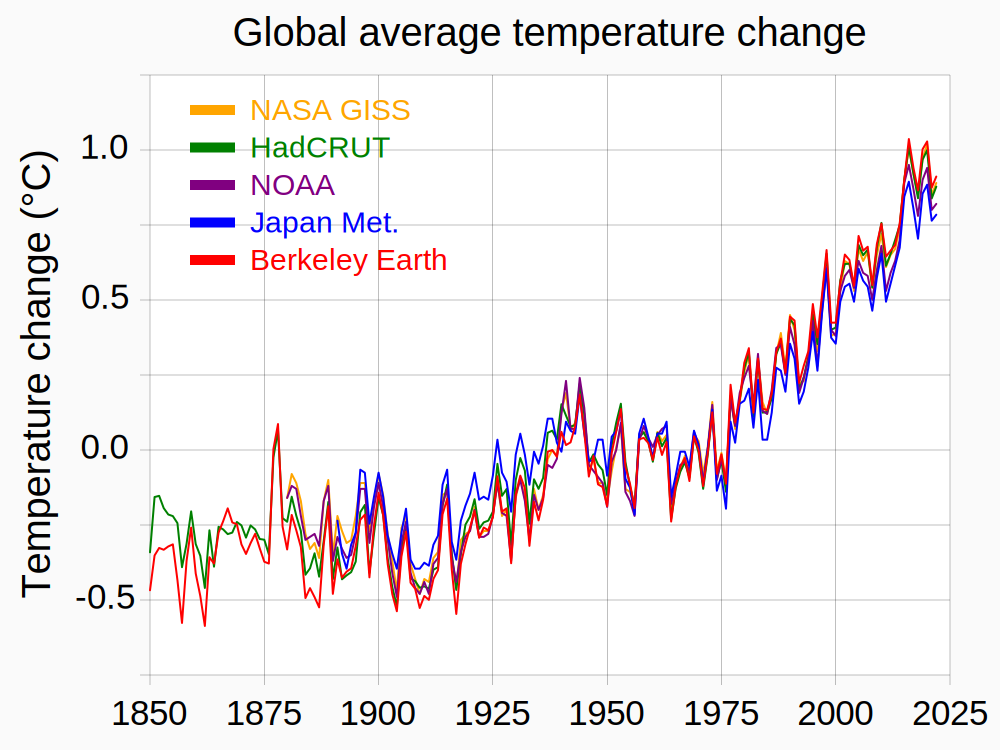
\includegraphics[width=2.08333in,height=\textheight,keepaspectratio]{index_files/mediabag/images/20200324_Global_average_temperature_-_NASA-GISS_HadCrut_NOAA_Japan_BerkeleyE.pdf}\end{footnotesize}}}
\item
  ice cores for the last 800,000 years
  {\marginnote{\begin{footnotesize}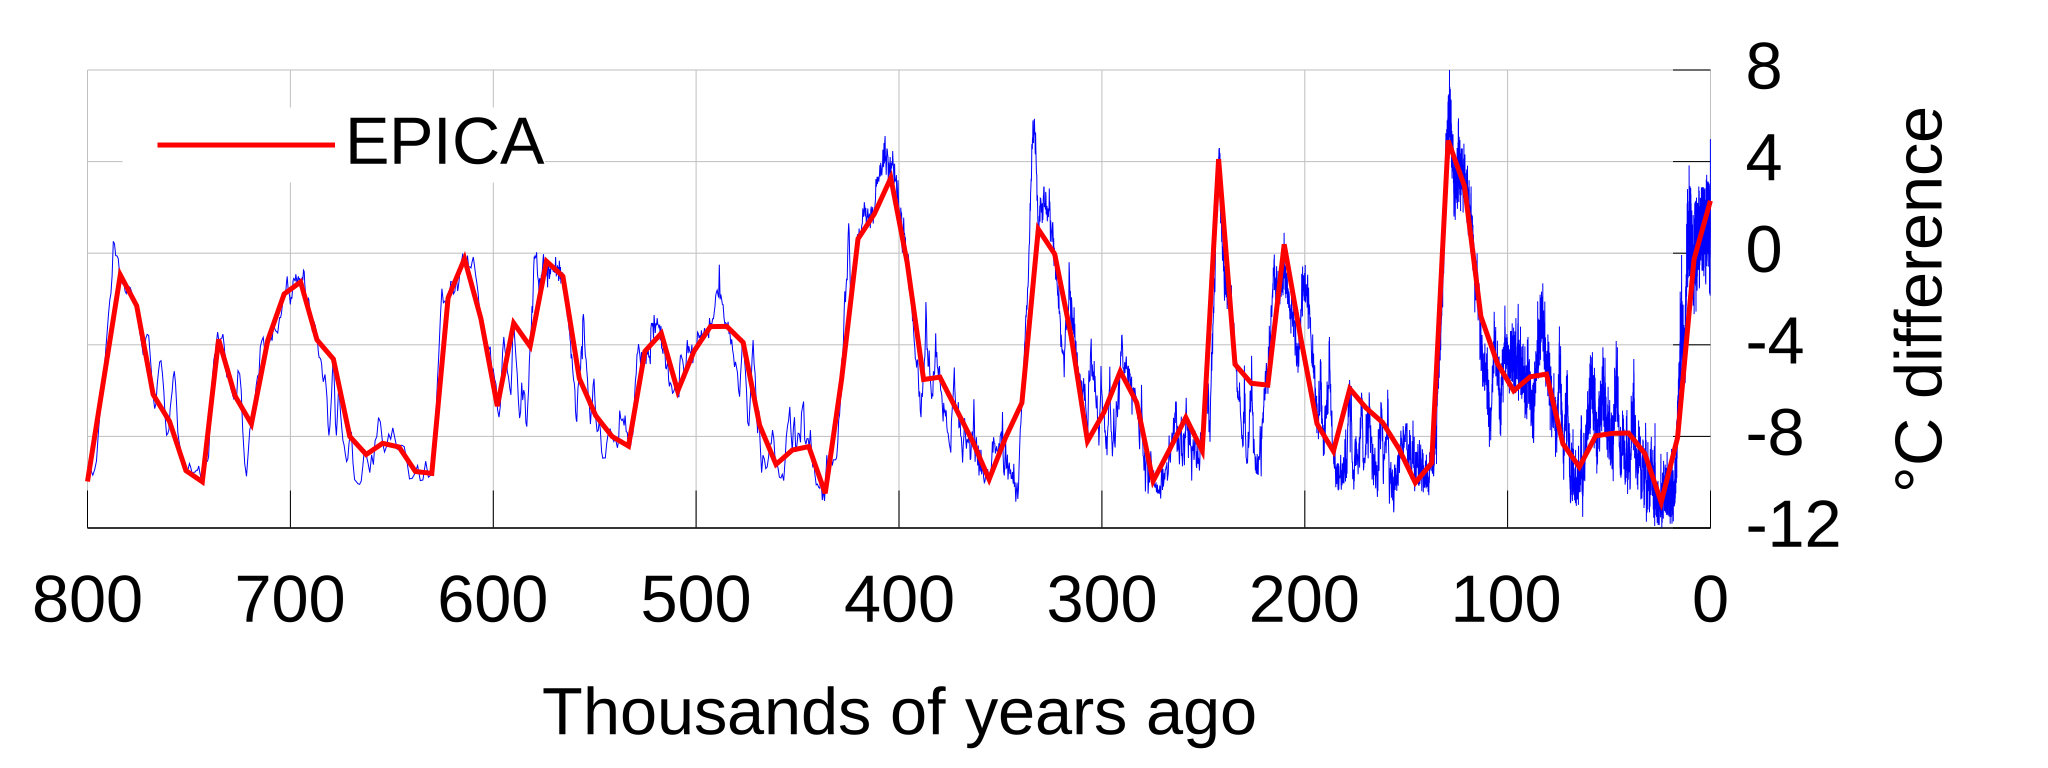
\includegraphics[width=2.08333in,height=\textheight,keepaspectratio]{index_files/mediabag/images/EPICA_temperature_plot.pdf}\end{footnotesize}}}
\item
  deep sea sediment oxygen 18 isotope fractation for the last 5 million
  years.
  {\marginnote{\begin{footnotesize}\pandocbounded{\includegraphics[keepaspectratio]{images/Five_Myr_Climate_Change.png}}\end{footnotesize}}}
  or yearly temperature data from 1850 till today based on
  meteorological readings. We can also consider Greenland ice core data
  covering 800,000 years.
\end{itemize}

One simple way is to model the yearly temperature as a random walk

i.e.~Each year is a Bernoulli trial where success is the temperature
getting warmer. We can then use the historical data since 1800 to
estimate theta the probability that we get warmer.

I suppose we can use a Binomial prior with parameters for alpha the
count of years the temperature increased and N for the total number of
years and p the probability the a given year is hotter than the
previous.
\end{solution}

\end{exercise}

\section{Data Analysis Example in R}\label{data-analysis-example-in-r}

Suppose we're giving two students a multiple-choice exam with 40
questions, where each question has four choices. We don't know how much
the students have studied for this exam, but we think that they'll do
better than just guessing randomly

\begin{enumerate}
\def\labelenumi{\arabic{enumi}.}
\tightlist
\item
  What are the parameters of interest?
\end{enumerate}

The parameters of interests are \(\theta_1 = true\) the probability that
the first student will answer a question correctly, \(\theta_2 = true\)
the probability that the second student will answer a question
correctly.

\begin{enumerate}
\def\labelenumi{\arabic{enumi}.}
\setcounter{enumi}{1}
\tightlist
\item
  What is our likelihood?
\end{enumerate}

The likelihood is \(\mathrm{Binomial}(40, \theta)\) if we assume that
each question is independent and that the probability a student gets
each question right is the same for all questions for that student.

\begin{enumerate}
\def\labelenumi{\arabic{enumi}.}
\setcounter{enumi}{2}
\tightlist
\item
  What prior should we use?
\end{enumerate}

The \textbf{Conjugate Prior} is a \textbf{Beta Distribution}. We can
plot the density with \texttt{dbeta}

\begin{Shaded}
\begin{Highlighting}[]
\NormalTok{theta }\OtherTok{=} \FunctionTok{seq}\NormalTok{(}\AttributeTok{from =} \DecValTok{0}\NormalTok{, }\AttributeTok{to =} \DecValTok{1}\NormalTok{, }\AttributeTok{by =} \FloatTok{0.1}\NormalTok{)}
\CommentTok{\# Uniform}
\FunctionTok{plot}\NormalTok{(theta, }\FunctionTok{dbeta}\NormalTok{(theta, }\DecValTok{1}\NormalTok{, }\DecValTok{1}\NormalTok{), }\AttributeTok{type =} \StringTok{\textquotesingle{}l\textquotesingle{}}\NormalTok{)}
\end{Highlighting}
\end{Shaded}

\pandocbounded{\includegraphics[keepaspectratio]{C1-L07_files/figure-pdf/C1-L07-1-1.pdf}}

\begin{Shaded}
\begin{Highlighting}[]
\CommentTok{\# Prior mean 2/3}
\FunctionTok{plot}\NormalTok{(theta, }\FunctionTok{dbeta}\NormalTok{(theta, }\DecValTok{4}\NormalTok{, }\DecValTok{2}\NormalTok{), }\AttributeTok{type =} \StringTok{\textquotesingle{}l\textquotesingle{}}\NormalTok{)}
\end{Highlighting}
\end{Shaded}

\pandocbounded{\includegraphics[keepaspectratio]{C1-L07_files/figure-pdf/C1-L07-1-2.pdf}}

\begin{Shaded}
\begin{Highlighting}[]
\CommentTok{\# Prior mean 2/3 but higher effect size (more concentrated at mean)}
\FunctionTok{plot}\NormalTok{(theta, }\FunctionTok{dbeta}\NormalTok{(theta, }\DecValTok{8}\NormalTok{, }\DecValTok{4}\NormalTok{), }\AttributeTok{type =} \StringTok{\textquotesingle{}l\textquotesingle{}}\NormalTok{)}
\end{Highlighting}
\end{Shaded}

\pandocbounded{\includegraphics[keepaspectratio]{C1-L07_files/figure-pdf/C1-L07-1-3.pdf}}

\begin{enumerate}
\def\labelenumi{\arabic{enumi}.}
\setcounter{enumi}{3}
\tightlist
\item
  What are the prior probabilities \(\mathbb{P}r(\theta > 0.25)\)?
  \(\mathbb{P}r(\theta > 0.5)\)? \(\mathbb{P}r(\theta > 0.8)\)?
\end{enumerate}

\begin{Shaded}
\begin{Highlighting}[]
\DecValTok{1} \SpecialCharTok{{-}} \FunctionTok{pbeta}\NormalTok{(}\FloatTok{0.25}\NormalTok{, }\DecValTok{8}\NormalTok{, }\DecValTok{4}\NormalTok{)}
\end{Highlighting}
\end{Shaded}

\begin{verbatim}
[1] 0.9988117
\end{verbatim}

\begin{Shaded}
\begin{Highlighting}[]
\CommentTok{\#[1] 0.998117}
\DecValTok{1} \SpecialCharTok{{-}} \FunctionTok{pbeta}\NormalTok{(}\FloatTok{0.5}\NormalTok{, }\DecValTok{8}\NormalTok{, }\DecValTok{4}\NormalTok{)}
\end{Highlighting}
\end{Shaded}

\begin{verbatim}
[1] 0.8867188
\end{verbatim}

\begin{Shaded}
\begin{Highlighting}[]
\CommentTok{\#[1] 0.8867188}
\DecValTok{1} \SpecialCharTok{{-}} \FunctionTok{pbeta}\NormalTok{(}\FloatTok{0.8}\NormalTok{, }\DecValTok{8}\NormalTok{, }\DecValTok{4}\NormalTok{)}
\end{Highlighting}
\end{Shaded}

\begin{verbatim}
[1] 0.1611392
\end{verbatim}

\begin{Shaded}
\begin{Highlighting}[]
\CommentTok{\#[1] 0.16113392}
\end{Highlighting}
\end{Shaded}

\begin{enumerate}
\def\labelenumi{\arabic{enumi}.}
\setcounter{enumi}{4}
\item
  Suppose the first student gets 33 questions right. What is the
  posterior distribution for \(\theta_1\) ?
  \(\mathbb{P}r(\theta > 0.25)\) ? \(\mathbb{P}r(\theta > 0.5)\) ?
  \(\mathbb{P}r(\theta > 0.8)\) ? What is the 95\% posterior credible
  interval for \(\theta_1\)?

  \[
  \text{Posterior} \sim Beta(8 + 33, 4 + 40 - 33) = Beta(41, 11)
  \]

  With a posterior mean of \(\frac{41}{41+11} = \frac{41}{52}\)
\end{enumerate}

We can plot the posterior distribution with the prior

\begin{Shaded}
\begin{Highlighting}[]
\FunctionTok{plot}\NormalTok{(theta, }\FunctionTok{dbeta}\NormalTok{(theta, }\DecValTok{41}\NormalTok{, }\DecValTok{11}\NormalTok{), }\AttributeTok{type =} \StringTok{\textquotesingle{}l\textquotesingle{}}\NormalTok{)}
\FunctionTok{lines}\NormalTok{(theta, }\FunctionTok{dbeta}\NormalTok{(theta, }\DecValTok{8}\NormalTok{ ,}\DecValTok{4}\NormalTok{), }\AttributeTok{lty =} \DecValTok{2}\NormalTok{) }\CommentTok{\#Dashed line for prior}
\end{Highlighting}
\end{Shaded}

\pandocbounded{\includegraphics[keepaspectratio]{C1-L07_files/figure-pdf/C1-L07-3-1.pdf}}

Posterior probabilities

\begin{Shaded}
\begin{Highlighting}[]
\DecValTok{1} \SpecialCharTok{{-}} \FunctionTok{pbeta}\NormalTok{(}\FloatTok{0.25}\NormalTok{, }\DecValTok{41}\NormalTok{, }\DecValTok{11}\NormalTok{)}
\end{Highlighting}
\end{Shaded}

\begin{verbatim}
[1] 1
\end{verbatim}

\begin{Shaded}
\begin{Highlighting}[]
\CommentTok{\#[1] 1}
\DecValTok{1} \SpecialCharTok{{-}} \FunctionTok{pbeta}\NormalTok{(}\FloatTok{0.5}\NormalTok{, }\DecValTok{41}\NormalTok{, }\DecValTok{11}\NormalTok{)}
\end{Highlighting}
\end{Shaded}

\begin{verbatim}
[1] 0.9999926
\end{verbatim}

\begin{Shaded}
\begin{Highlighting}[]
\CommentTok{\#[1] 0.9999926}
\DecValTok{1} \SpecialCharTok{{-}} \FunctionTok{pbeta}\NormalTok{(}\FloatTok{0.8}\NormalTok{, }\DecValTok{41}\NormalTok{, }\DecValTok{11}\NormalTok{)}
\end{Highlighting}
\end{Shaded}

\begin{verbatim}
[1] 0.4444044
\end{verbatim}

\begin{Shaded}
\begin{Highlighting}[]
\CommentTok{\#[1] 0.4444044}
\end{Highlighting}
\end{Shaded}

Equal-tailed 95\% credible interval

\begin{Shaded}
\begin{Highlighting}[]
\FunctionTok{qbeta}\NormalTok{(}\FloatTok{0.025}\NormalTok{, }\DecValTok{41}\NormalTok{, }\DecValTok{11}\NormalTok{)}
\end{Highlighting}
\end{Shaded}

\begin{verbatim}
[1] 0.6688426
\end{verbatim}

\begin{Shaded}
\begin{Highlighting}[]
\CommentTok{\#[1] 0.6688426}
\FunctionTok{qbeta}\NormalTok{(}\FloatTok{0.975}\NormalTok{, }\DecValTok{41}\NormalTok{, }\DecValTok{11}\NormalTok{)}
\end{Highlighting}
\end{Shaded}

\begin{verbatim}
[1] 0.8871094
\end{verbatim}

\begin{Shaded}
\begin{Highlighting}[]
\CommentTok{\#[1] 0.8871094}
\end{Highlighting}
\end{Shaded}

95\% confidence that \(\theta_1\) is between 0.67 and 0.89

\begin{enumerate}
\def\labelenumi{\arabic{enumi}.}
\setcounter{enumi}{5}
\tightlist
\item
  Suppose the second student gets 24 questions right. What is the
  posterior distribution for \(\theta_2\)?
  \(\mathbb{P}r(\theta > 0.25)\)? \(\mathbb{P}r(\theta > 0.5)\)?
  \(\mathbb{P}r(\theta > 0.8)\)? What is the 95\% posterior credible
  interval for \(\theta_2\)
\end{enumerate}

\[
\text{Posterior} \sim Beta(8 + 24, 4 + 40 - 24) = Beta(32, 20)
\]

With a posterior mean of \(\frac{32}{32+20} = \frac{32}{52}\)

We can plot the posterior distribution with the prior

\begin{Shaded}
\begin{Highlighting}[]
\FunctionTok{plot}\NormalTok{(theta, }\FunctionTok{dbeta}\NormalTok{(theta, }\DecValTok{32}\NormalTok{, }\DecValTok{20}\NormalTok{), }\AttributeTok{type =} \StringTok{\textquotesingle{}l\textquotesingle{}}\NormalTok{)}
\FunctionTok{lines}\NormalTok{(theta, }\FunctionTok{dbeta}\NormalTok{(theta, }\DecValTok{8}\NormalTok{ ,}\DecValTok{4}\NormalTok{), }\AttributeTok{lty =} \DecValTok{2}\NormalTok{) }\CommentTok{\#Dashed line for prior}
\end{Highlighting}
\end{Shaded}

\pandocbounded{\includegraphics[keepaspectratio]{C1-L07_files/figure-pdf/C1-L07-6-1.pdf}}

Posterior probabilities

\begin{Shaded}
\begin{Highlighting}[]
\DecValTok{1} \SpecialCharTok{{-}} \FunctionTok{pbeta}\NormalTok{(}\FloatTok{0.25}\NormalTok{, }\DecValTok{32}\NormalTok{, }\DecValTok{20}\NormalTok{)}
\end{Highlighting}
\end{Shaded}

\begin{verbatim}
[1] 1
\end{verbatim}

\begin{Shaded}
\begin{Highlighting}[]
\CommentTok{\#[1] 1}
\DecValTok{1} \SpecialCharTok{{-}} \FunctionTok{pbeta}\NormalTok{(}\FloatTok{0.5}\NormalTok{, }\DecValTok{32}\NormalTok{, }\DecValTok{20}\NormalTok{)}
\end{Highlighting}
\end{Shaded}

\begin{verbatim}
[1] 0.9540427
\end{verbatim}

\begin{Shaded}
\begin{Highlighting}[]
\CommentTok{\#[1] 0.9540427}
\DecValTok{1} \SpecialCharTok{{-}} \FunctionTok{pbeta}\NormalTok{(}\FloatTok{0.8}\NormalTok{, }\DecValTok{32}\NormalTok{, }\DecValTok{20}\NormalTok{)}
\end{Highlighting}
\end{Shaded}

\begin{verbatim}
[1] 0.00124819
\end{verbatim}

\begin{Shaded}
\begin{Highlighting}[]
\CommentTok{\#[1] 0.00124819}
\end{Highlighting}
\end{Shaded}

Equal-tailed 95\% credible interval

\begin{Shaded}
\begin{Highlighting}[]
\FunctionTok{qbeta}\NormalTok{(}\FloatTok{0.025}\NormalTok{, }\DecValTok{32}\NormalTok{, }\DecValTok{20}\NormalTok{)}
\end{Highlighting}
\end{Shaded}

\begin{verbatim}
[1] 0.4808022
\end{verbatim}

\begin{Shaded}
\begin{Highlighting}[]
\CommentTok{\#[1] 0.4808022}
\FunctionTok{qbeta}\NormalTok{(}\FloatTok{0.975}\NormalTok{, }\DecValTok{32}\NormalTok{, }\DecValTok{20}\NormalTok{)}
\end{Highlighting}
\end{Shaded}

\begin{verbatim}
[1] 0.7415564
\end{verbatim}

\begin{Shaded}
\begin{Highlighting}[]
\CommentTok{\#[1] 0.7415564}
\end{Highlighting}
\end{Shaded}

95\% confidence that \(\theta_1\) is between 0.48 and 0.74

\begin{enumerate}
\def\labelenumi{\arabic{enumi}.}
\setcounter{enumi}{6}
\tightlist
\item
  What is the posterior probability that \(\theta_1 > \theta_2\)?
\end{enumerate}

i.e., that the first student has a better chance of getting a question
right than the second student?

Estimate by simulation: draw 1,000 samples from each and see how often
we observe \(\theta_1 > \theta_2\)

\begin{Shaded}
\begin{Highlighting}[]
\NormalTok{theta1 }\OtherTok{=} \FunctionTok{rbeta}\NormalTok{(}\DecValTok{100000}\NormalTok{, }\DecValTok{41}\NormalTok{, }\DecValTok{11}\NormalTok{)}
\NormalTok{theta2 }\OtherTok{=} \FunctionTok{rbeta}\NormalTok{(}\DecValTok{100000}\NormalTok{, }\DecValTok{32}\NormalTok{, }\DecValTok{20}\NormalTok{)}
\FunctionTok{mean}\NormalTok{(theta1 }\SpecialCharTok{\textgreater{}}\NormalTok{ theta2)}
\end{Highlighting}
\end{Shaded}

\begin{verbatim}
[1] 0.97523
\end{verbatim}

\begin{Shaded}
\begin{Highlighting}[]
\CommentTok{\#[1] 0.975}
\end{Highlighting}
\end{Shaded}

\bookmarksetup{startatroot}

\chapter{Homework on Priors}\label{homework-on-priors}

For Questions Exercise~\ref{exr-priors-1}-Exercise~\ref{exr-priors-5},
consider the example of flipping a coin with unknown probability of
heads (\(\theta\)):

Suppose we use a Bernoulli likelihood for each coin flip,

i.e.,
\(f(y_i \mid \theta) = \theta^{y_i} (1-\theta)^{1-y_i} I_{\{ 0 \le \theta \le 1 \}}\)
for \(y_i=0\) or \(y_i=1\), and a uniform prior for \(\theta\).

\begin{exercise}[]\protect\hypertarget{exr-priors-1}{}\label{exr-priors-1}

{\marginnote{\begin{footnotesize}\textbf{flipping a
coin}\end{footnotesize}}}

What is the \emph{posterior distribution} for \(\theta\) if we observe
the following sequence: (T, T, T, T) where \textbf{H} denotes heads
\((Y=1)\) and \textbf{T} denotes tails \((Y=0)\)?

\end{exercise}

\begin{tcolorbox}[enhanced jigsaw, arc=.35mm, colback=white, title=\textcolor{quarto-callout-tip-color}{\faLightbulb}\hspace{0.5em}{Solution:}, toptitle=1mm, breakable, opacityback=0, bottomrule=.15mm, opacitybacktitle=0.6, colbacktitle=quarto-callout-tip-color!10!white, rightrule=.15mm, toprule=.15mm, left=2mm, titlerule=0mm, colframe=quarto-callout-tip-color-frame, coltitle=black, bottomtitle=1mm, leftrule=.75mm]

\begin{itemize}
\tightlist
\item[$\square$]
  Beta(1,4)
\item[$\square$]
  Beta(4,0)
\item[$\square$]
  Beta(0, 4)
\item[$\square$]
  Uniform(0,4)
\item[$\boxtimes$]
  Beta(1, 5)
\end{itemize}

This is the PDF of a Beta(1,5).

\end{tcolorbox}

\begin{exercise}[]\protect\hypertarget{exr-priors-2}{}\label{exr-priors-2}

Which of the following graphs depicts the posterior PDF of \(\theta\) if
we observe the sequence (T, T, T, T)? (You may want to use R to plot the
posterior.)

\end{exercise}

\begin{tcolorbox}[enhanced jigsaw, arc=.35mm, colback=white, title=\textcolor{quarto-callout-tip-color}{\faLightbulb}\hspace{0.5em}{Solution:}, toptitle=1mm, breakable, opacityback=0, bottomrule=.15mm, opacitybacktitle=0.6, colbacktitle=quarto-callout-tip-color!10!white, rightrule=.15mm, toprule=.15mm, left=2mm, titlerule=0mm, colframe=quarto-callout-tip-color-frame, coltitle=black, bottomtitle=1mm, leftrule=.75mm]

\begin{Shaded}
\begin{Highlighting}[]
\NormalTok{theta }\OtherTok{=} \FunctionTok{seq}\NormalTok{(}\AttributeTok{from =} \DecValTok{0}\NormalTok{, }\AttributeTok{to =} \DecValTok{1}\NormalTok{, }\AttributeTok{by =} \FloatTok{0.1}\NormalTok{)}
\CommentTok{\# Uniform}
\FunctionTok{plot}\NormalTok{(theta, }\FunctionTok{dbeta}\NormalTok{(theta, }\DecValTok{1}\NormalTok{, }\DecValTok{5}\NormalTok{), }\AttributeTok{type =} \StringTok{\textquotesingle{}l\textquotesingle{}}\NormalTok{)}
\end{Highlighting}
\end{Shaded}

\pandocbounded{\includegraphics[keepaspectratio]{C1-L07-Ex1_files/figure-pdf/C1-L07-Ex1-1-1.pdf}}

\end{tcolorbox}

\begin{exercise}[]\protect\hypertarget{exr-priors-3}{}\label{exr-priors-3}

What is the maximum likelihood estimate (MLE) of θ if we observe the
sequence (T, T, T, T)?

\end{exercise}

\begin{tcolorbox}[enhanced jigsaw, arc=.35mm, colback=white, title=\textcolor{quarto-callout-tip-color}{\faLightbulb}\hspace{0.5em}{Solution:}, toptitle=1mm, breakable, opacityback=0, bottomrule=.15mm, opacitybacktitle=0.6, colbacktitle=quarto-callout-tip-color!10!white, rightrule=.15mm, toprule=.15mm, left=2mm, titlerule=0mm, colframe=quarto-callout-tip-color-frame, coltitle=black, bottomtitle=1mm, leftrule=.75mm]

\begin{Shaded}
\begin{Highlighting}[]
\DecValTok{4}\SpecialCharTok{*}\DecValTok{0}\SpecialCharTok{/}\DecValTok{4}
\end{Highlighting}
\end{Shaded}

\begin{verbatim}
[1] 0
\end{verbatim}

The main issue here seems to be if we need to consider the prior in the
sample size ?

\end{tcolorbox}

\begin{exercise}[]\protect\hypertarget{exr-priors-4}{}\label{exr-priors-4}

What is the posterior mean estimate of \(\theta\) if we observe the
sequence (T, T, T, T)?

\end{exercise}

\begin{tcolorbox}[enhanced jigsaw, arc=.35mm, colback=white, title=\textcolor{quarto-callout-tip-color}{\faLightbulb}\hspace{0.5em}{Solution:}, toptitle=1mm, breakable, opacityback=0, bottomrule=.15mm, opacitybacktitle=0.6, colbacktitle=quarto-callout-tip-color!10!white, rightrule=.15mm, toprule=.15mm, left=2mm, titlerule=0mm, colframe=quarto-callout-tip-color-frame, coltitle=black, bottomtitle=1mm, leftrule=.75mm]

\begin{Shaded}
\begin{Highlighting}[]
\NormalTok{a}\OtherTok{=}\DecValTok{1}
\NormalTok{b}\OtherTok{=}\DecValTok{5}
\NormalTok{a}\SpecialCharTok{/}\NormalTok{(a}\SpecialCharTok{+}\NormalTok{b)}
\end{Highlighting}
\end{Shaded}

\begin{verbatim}
[1] 0.1666667
\end{verbatim}

\end{tcolorbox}

\begin{exercise}[]\protect\hypertarget{exr-priors-5}{}\label{exr-priors-5}

Use R or Excel to find the posterior probability that \(θ<0.5\) if we
observe the sequence (T,T,T,T).

\end{exercise}

\begin{tcolorbox}[enhanced jigsaw, arc=.35mm, colback=white, title=\textcolor{quarto-callout-tip-color}{\faLightbulb}\hspace{0.5em}{Solution:}, toptitle=1mm, breakable, opacityback=0, bottomrule=.15mm, opacitybacktitle=0.6, colbacktitle=quarto-callout-tip-color!10!white, rightrule=.15mm, toprule=.15mm, left=2mm, titlerule=0mm, colframe=quarto-callout-tip-color-frame, coltitle=black, bottomtitle=1mm, leftrule=.75mm]

\begin{Shaded}
\begin{Highlighting}[]
\NormalTok{a}\OtherTok{=}\DecValTok{1}
\NormalTok{b}\OtherTok{=}\DecValTok{5}
\FunctionTok{pbeta}\NormalTok{(}\AttributeTok{q=}\FloatTok{0.5}\NormalTok{, }\AttributeTok{shape1=}\NormalTok{a, }\AttributeTok{shape2=}\NormalTok{b)}
\end{Highlighting}
\end{Shaded}

\begin{verbatim}
[1] 0.96875
\end{verbatim}

\end{tcolorbox}

For Questions Exercise~\ref{exr-priors-6}-Exercise~\ref{exr-priors-9},
consider the following scenario:

{\marginnote{\begin{footnotesize}Chemical refinement\end{footnotesize}}}
An engineer wants to assess the reliability of a new chemical refinement
process by measuring \(\theta\), the proportion of samples that fail a
battery of tests. These tests are expensive, and the budget only allows
20 tests on randomly selected samples. Assuming each test is
independent, she assigns a binomial likelihood where X counts the
samples which fail. Historically, new processes pass about half of the
time, so she assigns a \(\text{Beta}(2,2)\) prior for \(\theta\) (prior
mean 0.5 and prior sample size 4). The outcome of the tests is 6 fails
and 14 passes.

\begin{exercise}[]\protect\hypertarget{exr-priors-6}{}\label{exr-priors-6}

{\marginnote{\begin{footnotesize}Chemical refinement\end{footnotesize}}}

What is the posterior distribution for θ? Beta(8,16)

\end{exercise}

\begin{tcolorbox}[enhanced jigsaw, arc=.35mm, colback=white, title=\textcolor{quarto-callout-tip-color}{\faLightbulb}\hspace{0.5em}{Solution:}, toptitle=1mm, breakable, opacityback=0, bottomrule=.15mm, opacitybacktitle=0.6, colbacktitle=quarto-callout-tip-color!10!white, rightrule=.15mm, toprule=.15mm, left=2mm, titlerule=0mm, colframe=quarto-callout-tip-color-frame, coltitle=black, bottomtitle=1mm, leftrule=.75mm]

\begin{itemize}
\tightlist
\item[$\boxtimes$]
  Beta(8,16)
\item[$\square$]
  Beta(14,6)
\item[$\square$]
  Beta(6,14)
\item[$\square$]
  Beta(6, 20)
\item[$\square$]
  Beta(16,8)
\end{itemize}

\end{tcolorbox}

\begin{exercise}[]\protect\hypertarget{exr-priors-7}{}\label{exr-priors-7}

{\marginnote{\begin{footnotesize}Chemical refinement\end{footnotesize}}}

Use R to calculate the upper end of an equal-tailed 95\% credible
interval for θ. Round your answer to two decimal places.

\end{exercise}

\begin{tcolorbox}[enhanced jigsaw, arc=.35mm, colback=white, title=\textcolor{quarto-callout-tip-color}{\faLightbulb}\hspace{0.5em}{Solution:}, toptitle=1mm, breakable, opacityback=0, bottomrule=.15mm, opacitybacktitle=0.6, colbacktitle=quarto-callout-tip-color!10!white, rightrule=.15mm, toprule=.15mm, left=2mm, titlerule=0mm, colframe=quarto-callout-tip-color-frame, coltitle=black, bottomtitle=1mm, leftrule=.75mm]

\begin{Shaded}
\begin{Highlighting}[]
\NormalTok{a}\OtherTok{=}\DecValTok{8}
\NormalTok{b}\OtherTok{=}\DecValTok{16}
\FunctionTok{qbeta}\NormalTok{(}\AttributeTok{p=}\FloatTok{0.975}\NormalTok{, }\AttributeTok{shape1=}\NormalTok{a, }\AttributeTok{shape2=}\NormalTok{b)}
\end{Highlighting}
\end{Shaded}

\begin{verbatim}
[1] 0.5291917
\end{verbatim}

where probability=0.975, alpha=8, and beta=16.

\end{tcolorbox}

\begin{exercise}[]\protect\hypertarget{exr-priors-8}{}\label{exr-priors-8}

{\marginnote{\begin{footnotesize}Chemical refinement\end{footnotesize}}}

The engineer tells you that the process is considered promising and can
proceed to another phase of testing if we are 90\% sure that the failure
rate is less than .35.

Calculate the posterior probability
\(\mathbb{P}r(\theta < .35 \mid x)\). In your role as the statistician,
would you say that this new chemical should pass?

\end{exercise}

\begin{tcolorbox}[enhanced jigsaw, arc=.35mm, colback=white, title=\textcolor{quarto-callout-tip-color}{\faLightbulb}\hspace{0.5em}{Solution:}, toptitle=1mm, breakable, opacityback=0, bottomrule=.15mm, opacitybacktitle=0.6, colbacktitle=quarto-callout-tip-color!10!white, rightrule=.15mm, toprule=.15mm, left=2mm, titlerule=0mm, colframe=quarto-callout-tip-color-frame, coltitle=black, bottomtitle=1mm, leftrule=.75mm]

\begin{Shaded}
\begin{Highlighting}[]
\NormalTok{a}\OtherTok{=}\DecValTok{8}
\NormalTok{b}\OtherTok{=}\DecValTok{16}
\FunctionTok{pbeta}\NormalTok{(}\AttributeTok{q=}\FloatTok{0.35}\NormalTok{, }\AttributeTok{shape1=}\NormalTok{a, }\AttributeTok{shape2=}\NormalTok{b)}
\end{Highlighting}
\end{Shaded}

\begin{verbatim}
[1] 0.586431
\end{verbatim}

\begin{itemize}
\tightlist
\item[$\square$]
  Yes, \(\mathbb{P}r(θ<.35 \mid x_1,x_2)≥0.9\).
\item[$\boxtimes$]
  No, \(\mathbb{P}r(θ<.35 \mid x_1,x_2)<0.9\).
\end{itemize}

\end{tcolorbox}

\begin{exercise}[]\protect\hypertarget{exr-priors-9}{}\label{exr-priors-9}

{\marginnote{\begin{footnotesize}Chemical refinement\end{footnotesize}}}

It is discovered that the budget will allow five more samples to be
tested. These tests are conducted and none of them fail.

Calculate the new posterior probability
\(\mathbb{P}r(\theta < .35 \mid x_1, x_2)\). In your role as the
statistician, would you say that this new chemical should pass (with the
same requirement as in the previous question)?

\end{exercise}

\begin{tcolorbox}[enhanced jigsaw, arc=.35mm, colback=white, title=\textcolor{quarto-callout-tip-color}{\faLightbulb}\hspace{0.5em}{Solution:}, toptitle=1mm, breakable, opacityback=0, bottomrule=.15mm, opacitybacktitle=0.6, colbacktitle=quarto-callout-tip-color!10!white, rightrule=.15mm, toprule=.15mm, left=2mm, titlerule=0mm, colframe=quarto-callout-tip-color-frame, coltitle=black, bottomtitle=1mm, leftrule=.75mm]

Hint: You can use the posterior from the previous analysis as the prior
for this analysis. Assuming independence of tests, this yields the same
posterior as the analysis in which we begin with the Beta(2,2) prior and
use all 25 tests as the data.

\begin{Shaded}
\begin{Highlighting}[]
\NormalTok{a}\OtherTok{=}\DecValTok{8}
\NormalTok{b}\OtherTok{=}\DecValTok{16}
\NormalTok{a2}\OtherTok{=}\NormalTok{a}\SpecialCharTok{+}\DecValTok{0}
\NormalTok{b2}\OtherTok{=}\NormalTok{b}\SpecialCharTok{+}\DecValTok{5}
\FunctionTok{pbeta}\NormalTok{(}\AttributeTok{q=}\FloatTok{0.35}\NormalTok{, }\AttributeTok{shape1=}\NormalTok{a2, }\AttributeTok{shape2=}\NormalTok{b2)}
\end{Highlighting}
\end{Shaded}

\begin{verbatim}
[1] 0.8179064
\end{verbatim}

where x=0.5, alpha=8, beta=21, and cumulative=TRUE.

\begin{itemize}
\tightlist
\item[$\square$]
  Yes, \(\mathbb{P}r(θ<.35 \mid x)≥0.9\).
\item[$\boxtimes$]
  No, \(\mathbb{P}r(θ<.35 \mid x)<0.9\).
\end{itemize}

\end{tcolorbox}

\begin{exercise}[]\protect\hypertarget{exr-priors-10}{}\label{exr-priors-10}

let \(X \mid \theta \sim \text{Binomial}(9, \theta)\) and assume a
\(\text{Beta}(\alpha,\beta)\) prior for \(\theta\). Suppose your prior
guess (prior expectation) for \(\theta\) is 0.4 and you wish to use a
prior effective sample size of 5, what values of \(α\) and \(β\) should
you use?

\end{exercise}

\begin{tcolorbox}[enhanced jigsaw, arc=.35mm, colback=white, title=\textcolor{quarto-callout-tip-color}{\faLightbulb}\hspace{0.5em}{Solution:}, toptitle=1mm, breakable, opacityback=0, bottomrule=.15mm, opacitybacktitle=0.6, colbacktitle=quarto-callout-tip-color!10!white, rightrule=.15mm, toprule=.15mm, left=2mm, titlerule=0mm, colframe=quarto-callout-tip-color-frame, coltitle=black, bottomtitle=1mm, leftrule=.75mm]

\begin{itemize}
\tightlist
\item[$\square$]
  \(α=4, β=6\)
\item[$\square$]
  \(α=4, β=10\)
\item[$\square$]
  \(α=2, β=5\)
\item[$\boxtimes$]
  \(α=2, β=3\)
\end{itemize}

Here \(α+β=5\) and \(\frac{\alpha}{\alpha+\beta}\) =0.4.

\end{tcolorbox}

\bookmarksetup{startatroot}

\chapter{M3L8 - Poisson Data}\label{m3l8---poisson-data}

Bayesian Statistics: From Concept to Data Analysis

\hfill\break

\begin{marginfigure}

\centering{

\includegraphics[width=2.08333in,height=\textheight,keepaspectratio]{images/c1l08-ss-01-poisson-data.png}

}

\caption{\label{fig-poisson-likelihood-gamma-prior}Poisson likelihood
with a Gamma prior}

\end{marginfigure}%

\phantomsection\label{exp-chocolate-chip}
\subsection{Poisson - Chocolate Chip
Cookie}\label{poisson---chocolate-chip-cookie}

In mass-produced chocolate chip cookies, they make a large amount of
dough; mix in a large number of chips; then chunk out the individual
cookies. In this process, the number of chips per cookie approximately
follows a \textbf{Poisson distribution}.

If we were to assume that chips have no volume, then this would be
exactly a \emph{Poisson process} and follow exactly a \emph{Poisson
distribution}. In practice, since chips are not that small, so they
follow approximately a Poisson distribution for the number of chips per
cookie.

\begin{equation}\phantomsection\label{eq-poisson}{
Y_i \sim \mathrm{Poisson}(\lambda)
}\end{equation}

{\marginnote{\begin{footnotesize}\textbf{What is the likelihood of the
data?}\end{footnotesize}}} The likelihood of the data is given by the
Poisson distribution.

\[
\begin{aligned}
{\color{red}f(y \mid \lambda) = \frac{\lambda^{\sum{y_i}}e^{-n\lambda}}{\prod_{i = 1}^n{y_i!}}} \quad \forall (\lambda > 0) && \text{ Poisson Likelihood } 
\end{aligned}
\]

{\marginnote{\begin{footnotesize}\textbf{What type of prior should we
put on} \(\lambda\) ?\end{footnotesize}}} It would be convenient if we
could put a \emph{conjugate prior}. What distribution looks like
\(\lambda\) raised to a power and \(e\) raised to a negative power?

For this, we're going to use a Gamma prior.

\begin{equation}\phantomsection\label{eq-gamma-prior}{
\begin{aligned} \lambda &\sim \mathrm{Gamma}(\alpha, \beta) && \text{Gamma Prior} \\ \color{green}{ f(\lambda)} &= \color{green}{\frac{\beta^\alpha}{\Gamma(\alpha)}\lambda^{\alpha - 1}e^{-\beta\lambda}} && \text{subst. Gamma PDF} \end{aligned}
}\end{equation}

{\marginnote{\begin{footnotesize}\textbf{What is the
posterior?}\end{footnotesize}}} We can use Bayes theorem to find the
posterior.

\begin{equation}\phantomsection\label{eq-posterior}{
\begin{aligned} {\color{blue}f(\lambda \mid y)} &\propto \color{red}{ f(y \mid \lambda)} \color{green}{ f(\lambda)} && \text{Bayes without the denominator} \\ &\propto \color{red}{\lambda^{\sum{y_i}}e^{-n\lambda}}\color{green}{\lambda^{\alpha - 1}e^{-\beta \lambda} } && \text{subst. Likelihood and Prior} 
\\ & \propto { \color{blue} \lambda^{\alpha + \sum{y_i} - 1}e^{-(\beta + n)\lambda} } && \text{collecting terms}
\\ & \propto { \color{blue} \mathrm{Gamma}(\alpha + \sum{y_i}, \beta + n)}
\end{aligned} 
}\end{equation}

{\marginnote{\begin{footnotesize}\textbf{What is the posterior
distribution?}\end{footnotesize}}} The posterior is a Gamma distribution
with parameters \(\alpha + \sum{y_i}\) and \(\beta + n\).

Thus we can see that the posterior is a Gamma Distribution

\begin{equation}\phantomsection\label{eq-posterior-gamma}{
\lambda \mid y \sim \mathrm{Gamma}(\alpha + \sum{y_i}, \beta + n)
}\end{equation}

{\marginnote{\begin{footnotesize}\textbf{What is the posterior
mean?}\end{footnotesize}}} The posterior mean of a Gamma distribution is
given by

\hl{The mean of Gamma under this parameterization is:}
\(\frac{\alpha}{\beta}\)

The posterior mean is going to be

\begin{equation}\phantomsection\label{eq-posterior-mean}{
\begin{aligned}
{\color{blue}\mu_{\lambda}} &= \frac{\alpha + \sum{y_i}}{\beta + n} && \text{(Posterior Mean)} \\
posterior_{\mu} 
&= \frac{\alpha + \sum{y_i}}{\beta + n} \\
&= \frac{\beta}{\beta + n}\frac{\alpha}{\beta} + \frac{n}{\beta + n}\frac{\sum{y_i}}{n} \\
& \propto  \beta \cdot \mu_\text{prior} + n\cdot \mu_\text{data}
\end{aligned}
}\end{equation}

{\marginnote{\begin{footnotesize}\textbf{What is the posterior
variance?}\end{footnotesize}}} The posterior variance of a Gamma
distribution is given by

As you can see here the posterior mean of the Gamma distribution is also
the weighted average of the prior mean and the data mean.

Therefore, \hl{the effective sample size (ESS) of the Gamma prior is}
\(\beta\)

\begin{tcolorbox}[enhanced jigsaw, arc=.35mm, colback=white, title=\textcolor{quarto-callout-tip-color}{\faLightbulb}\hspace{0.5em}{Prior Elicitation of Gamma Hyper-parameters}, toptitle=1mm, breakable, opacityback=0, bottomrule=.15mm, opacitybacktitle=0.6, colbacktitle=quarto-callout-tip-color!10!white, rightrule=.15mm, toprule=.15mm, left=2mm, titlerule=0mm, colframe=quarto-callout-tip-color-frame, coltitle=black, bottomtitle=1mm, leftrule=.75mm]

Here are two strategies for choose the \emph{hyper-parameters}
\(\alpha\) and \(\beta\)

\begin{enumerate}
\def\labelenumi{\arabic{enumi}.}
\tightlist
\item
  \hl{An \emph{informative prior} with a prior mean guess of}
  \(\mu=\frac{a}{b}\) e.g.~what is the average number of chips per
  cookie?

  \begin{itemize}
  \tightlist
  \item
    Next we need another piece of knowledge to pinpoint both parameters.
  \item
    \hl{Can you estimate the error for the mean? I.e. what do you think
    the \emph{standard deviation} is? Since for the Gamma prior}
  \item
    \hl{What is the effective sample size} \(\text{ESS}=\beta\) ?
  \item
    \hl{How many units of information do you think we have in our prior
    v.s. our data points ?} \(\sigma = \frac{ \sqrt{\alpha} }{\beta}\)
  \end{itemize}
\item
  \hl{A \emph{vague prior} \index{vague prior} refers to one that's
  relatively flat across much of the space.}

  \begin{itemize}
  \tightlist
  \item
    For a \emph{Gamma prior} we can choose
    \(\Gamma(\epsilon, \epsilon)\) where \(\epsilon\) is small and
    strictly positive. This would create a distribution with a
    \(\mu = 1\) and a huge \(\sigma\) stretching across the whole space.
    And the \emph{effective sample size} will also be \(\epsilon\) Hence
    the posterior will be largely driven by the data and very little by
    the prior.
  \end{itemize}
\end{enumerate}

\end{tcolorbox}

The first strategy with a mean and an ESS will be used in numerous
models going forward so it is best to remember these two strategies!

\bookmarksetup{startatroot}

\chapter{Homework on Poisson Data}\label{homework-on-poisson-data}

Bayesian Statistics: From Concept to Data Analysis

\hfill\break

For Questions Exercise~\ref{exr-poisson-1}-Exercise~\ref{exr-poisson-8},
consider the chocolate chip cookie example from the lesson
{\marginnote{\begin{footnotesize}\textbf{Cookies}\end{footnotesize}}}

As in the lesson, we used a \textbf{Poisson likelihood} to model the
number of chips per cookie, and a conjugate gamma prior for \(\lambda\),
the expected number of chips per cookie.

Suppose your prior expectation for \(\lambda\) is 8.

\begin{exercise}[]\protect\hypertarget{exr-poisson-1}{}\label{exr-poisson-1}

{\marginnote{\begin{footnotesize}\textbf{Cookies}\end{footnotesize}}}

The conjugate prior with mean 8 and effective sample size of 2 is
\(Gamma(\alpha,2)\). Find the value of \(\alpha\).

\end{exercise}

\begin{tcolorbox}[enhanced jigsaw, arc=.35mm, colback=white, title=\textcolor{quarto-callout-tip-color}{\faLightbulb}\hspace{0.5em}{Solution:}, toptitle=1mm, breakable, opacityback=0, bottomrule=.15mm, opacitybacktitle=0.6, colbacktitle=quarto-callout-tip-color!10!white, rightrule=.15mm, toprule=.15mm, left=2mm, titlerule=0mm, colframe=quarto-callout-tip-color-frame, coltitle=black, bottomtitle=1mm, leftrule=.75mm]

if \(X \sim \mathrm{Gamma}(a,b)\) the mean for \(X\) is \(\frac{a}{b}\)

\[
\begin{aligned}
8 &= \frac{\alpha}{\beta}=\frac{\alpha}{2} \\ 
\implies \alpha&=16
\end{aligned}
\]

\end{tcolorbox}

\begin{exercise}[]\protect\hypertarget{exr-poisson-2}{}\label{exr-poisson-2}

{\marginnote{\begin{footnotesize}\textbf{Cookies}\end{footnotesize}}}

The conjugate prior with mean 8 and standard deviation 1 is

\end{exercise}

\begin{tcolorbox}[enhanced jigsaw, arc=.35mm, colback=white, title=\textcolor{quarto-callout-tip-color}{\faLightbulb}\hspace{0.5em}{Solution:}, toptitle=1mm, breakable, opacityback=0, bottomrule=.15mm, opacitybacktitle=0.6, colbacktitle=quarto-callout-tip-color!10!white, rightrule=.15mm, toprule=.15mm, left=2mm, titlerule=0mm, colframe=quarto-callout-tip-color-frame, coltitle=black, bottomtitle=1mm, leftrule=.75mm]

\[
\begin{aligned}
sd &= \frac{\sqrt{\alpha}}{8}= \frac{\sqrt{64}}{8} so\\ 
a &= 64
\end{aligned}
\]

\end{tcolorbox}

\begin{exercise}[]\protect\hypertarget{exr-poisson-3}{}\label{exr-poisson-3}

{\marginnote{\begin{footnotesize}\textbf{Cookies}\end{footnotesize}}}

Suppose you are not very confident in your prior guess of 8, so you want
to use a prior effective sample size of 1/100 cookies. Then the
conjugate prior is Gamma(a,0.01). Find the value of a

\end{exercise}

\begin{tcolorbox}[enhanced jigsaw, arc=.35mm, colback=white, title=\textcolor{quarto-callout-tip-color}{\faLightbulb}\hspace{0.5em}{Solution:}, toptitle=1mm, breakable, opacityback=0, bottomrule=.15mm, opacitybacktitle=0.6, colbacktitle=quarto-callout-tip-color!10!white, rightrule=.15mm, toprule=.15mm, left=2mm, titlerule=0mm, colframe=quarto-callout-tip-color-frame, coltitle=black, bottomtitle=1mm, leftrule=.75mm]

\(a=8\)

\[
\begin{aligned}
8 &= \frac{\alpha}{\beta} \\
  &=\frac{\alpha}{0.01} \\ 
\implies a &= 0.08
\end{aligned}
\]

\end{tcolorbox}

\begin{exercise}[]\protect\hypertarget{exr-poisson-4}{}\label{exr-poisson-4}

{\marginnote{\begin{footnotesize}\textbf{Cookies}\end{footnotesize}}}

Suppose you decide on the prior \(\mathrm{Gamma}(8, 1)\), which has a
prior mean of 8 and an effective sample size of 1 cookie.

We collect data, by sampling five cookies and counting the chips in
each. We find 9, 12, 10, 15, and 13 chips.

What is the posterior distribution for \(\lambda\)?

\end{exercise}

\begin{tcolorbox}[enhanced jigsaw, arc=.35mm, colback=white, title=\textcolor{quarto-callout-tip-color}{\faLightbulb}\hspace{0.5em}{Solution:}, toptitle=1mm, breakable, opacityback=0, bottomrule=.15mm, opacitybacktitle=0.6, colbacktitle=quarto-callout-tip-color!10!white, rightrule=.15mm, toprule=.15mm, left=2mm, titlerule=0mm, colframe=quarto-callout-tip-color-frame, coltitle=black, bottomtitle=1mm, leftrule=.75mm]

\[
\begin{aligned}
\lambda \mid y &\sim \Gamma(\alpha + \sum{y_i}, \beta + n) \\
               &= \mathrm{Gamma}(8 + (9+12+10+15+13),1+5) \\
               &= \mathrm{Gamma}(67,6)
\end{aligned}
\]

\end{tcolorbox}

\begin{exercise}[]\protect\hypertarget{exr-poisson-5}{}\label{exr-poisson-5}

{\marginnote{\begin{footnotesize}\textbf{Cookies}\end{footnotesize}}}

Continuing Exercise~\ref{exr-poisson-4}, what of the following graphs
shows the prior density (dotted line) and posterior density (solid line)
of \(\lambda\)?

\end{exercise}

\begin{tcolorbox}[enhanced jigsaw, arc=.35mm, colback=white, title=\textcolor{quarto-callout-tip-color}{\faLightbulb}\hspace{0.5em}{Solution:}, toptitle=1mm, breakable, opacityback=0, bottomrule=.15mm, opacitybacktitle=0.6, colbacktitle=quarto-callout-tip-color!10!white, rightrule=.15mm, toprule=.15mm, left=2mm, titlerule=0mm, colframe=quarto-callout-tip-color-frame, coltitle=black, bottomtitle=1mm, leftrule=.75mm]

\begin{Shaded}
\begin{Highlighting}[]
\CommentTok{\# Generate x{-}values}
\NormalTok{x }\OtherTok{\textless{}{-}} \FunctionTok{seq}\NormalTok{(}\DecValTok{0}\NormalTok{, }\DecValTok{20}\NormalTok{, }\AttributeTok{length.out =} \DecValTok{1000}\NormalTok{)}

\CommentTok{\# posterior parameters}
\NormalTok{shape }\OtherTok{\textless{}{-}} \FloatTok{67.}
\NormalTok{scale }\OtherTok{\textless{}{-}} \FloatTok{6.}
\CommentTok{\# Generate y{-}values for posterior using dgamma}
\NormalTok{y\_post }\OtherTok{\textless{}{-}} \FunctionTok{dgamma}\NormalTok{(x, shape, scale)}
\CommentTok{\# prior parameters}
\NormalTok{shape }\OtherTok{\textless{}{-}} \FloatTok{16.}
\NormalTok{scale }\OtherTok{\textless{}{-}} \DecValTok{2}
\CommentTok{\# Generate y{-}values for prior using dgamma}
\NormalTok{y\_prior }\OtherTok{\textless{}{-}} \FunctionTok{dgamma}\NormalTok{(x, shape, scale)}

\CommentTok{\# Plot the distribution}

\FunctionTok{plot}\NormalTok{(x, y\_post, }\AttributeTok{type =} \StringTok{"l"}\NormalTok{, }\AttributeTok{xlab =} \FunctionTok{expression}\NormalTok{(theta), }\AttributeTok{ylab =} \FunctionTok{expression}\NormalTok{(}\FunctionTok{paste}\NormalTok{(}\StringTok{"f("}\NormalTok{,theta,}\StringTok{"|"}\NormalTok{, x,}\StringTok{")"}\NormalTok{)),  }\AttributeTok{main =} \StringTok{"Gamma Distribution"}\NormalTok{, }\AttributeTok{xlim =} \FunctionTok{c}\NormalTok{(}\DecValTok{0}\NormalTok{, }\DecValTok{20}\NormalTok{),}\AttributeTok{lty=}\DecValTok{1}\NormalTok{,}\AttributeTok{col=}\StringTok{\textquotesingle{}blue\textquotesingle{}}\NormalTok{)}
\FunctionTok{lines}\NormalTok{(x, y\_prior, }\AttributeTok{lty=}\DecValTok{3}\NormalTok{,}\AttributeTok{col=}\StringTok{\textquotesingle{}red\textquotesingle{}}\NormalTok{)}
\FunctionTok{legend}\NormalTok{(}\DecValTok{1}\NormalTok{,}\DecValTok{20}\NormalTok{,}\AttributeTok{legend=}\FunctionTok{c}\NormalTok{(}\StringTok{"prior"}\NormalTok{,}\StringTok{"posterior"}\NormalTok{), }\AttributeTok{col=}\FunctionTok{c}\NormalTok{(}\StringTok{"blue"}\NormalTok{,}\StringTok{"red"}\NormalTok{), }\AttributeTok{lty=}\FunctionTok{c}\NormalTok{(}\DecValTok{1}\NormalTok{,}\DecValTok{3}\NormalTok{), }\AttributeTok{ncol=}\DecValTok{1}\NormalTok{)}
\end{Highlighting}
\end{Shaded}

\begin{figure}[H]

\centering{

\pandocbounded{\includegraphics[keepaspectratio]{C1-L08-Ex1_files/figure-pdf/fig-poisson-plot-1.pdf}}

}

\caption{\label{fig-poisson-plot}}

\end{figure}%

\end{tcolorbox}

\begin{exercise}[]\protect\hypertarget{exr-poisson-6}{}\label{exr-poisson-6}

{\marginnote{\begin{footnotesize}\textbf{Cookies}\end{footnotesize}}}

Continuing Exercise~\ref{exr-poisson-4}, what is the posterior mean for
λ? Round your answer to one decimal place.

\end{exercise}

\begin{tcolorbox}[enhanced jigsaw, arc=.35mm, colback=white, title=\textcolor{quarto-callout-tip-color}{\faLightbulb}\hspace{0.5em}{Solution:}, toptitle=1mm, breakable, opacityback=0, bottomrule=.15mm, opacitybacktitle=0.6, colbacktitle=quarto-callout-tip-color!10!white, rightrule=.15mm, toprule=.15mm, left=2mm, titlerule=0mm, colframe=quarto-callout-tip-color-frame, coltitle=black, bottomtitle=1mm, leftrule=.75mm]

\[
posterior_{mean} = \frac{\alpha + \sum{y_i}}{\beta + n} 
\\= \frac{8 + (9+12+10+15+13)}{1 + 5} = 67/6=11.1667=11.2
\]

\end{tcolorbox}

\begin{exercise}[]\protect\hypertarget{exr-poisson-7}{}\label{exr-poisson-7}

{\marginnote{\begin{footnotesize}\textbf{Cookies}\end{footnotesize}}}

Continuing Exercise~\ref{exr-poisson-4}, use R or Excel to find the
lower end of a 90\% equal-tailed credible interval for λ.

\end{exercise}

\begin{tcolorbox}[enhanced jigsaw, arc=.35mm, colback=white, title=\textcolor{quarto-callout-tip-color}{\faLightbulb}\hspace{0.5em}{Solution:}, toptitle=1mm, breakable, opacityback=0, bottomrule=.15mm, opacitybacktitle=0.6, colbacktitle=quarto-callout-tip-color!10!white, rightrule=.15mm, toprule=.15mm, left=2mm, titlerule=0mm, colframe=quarto-callout-tip-color-frame, coltitle=black, bottomtitle=1mm, leftrule=.75mm]

\begin{Shaded}
\begin{Highlighting}[]
\CommentTok{\# Set parameters}
\NormalTok{shape }\OtherTok{\textless{}{-}} \DecValTok{8}\SpecialCharTok{+}\DecValTok{59}
\NormalTok{rate }\OtherTok{\textless{}{-}} \DecValTok{1}\SpecialCharTok{+}\DecValTok{5}


\CommentTok{\# Calculate 90\% equal{-}tailed credible interval}
\NormalTok{lower }\OtherTok{\textless{}{-}} \FunctionTok{qgamma}\NormalTok{(}\FloatTok{0.05}\NormalTok{, }\AttributeTok{shape =}\NormalTok{ shape, }\AttributeTok{rate =}\NormalTok{ rate)}
\NormalTok{upper }\OtherTok{\textless{}{-}} \FunctionTok{qgamma}\NormalTok{(}\FloatTok{0.95}\NormalTok{, }\AttributeTok{shape =}\NormalTok{ shape, }\AttributeTok{rate =}\NormalTok{ rate)}

\CommentTok{\# Print interval}
\FunctionTok{cat}\NormalTok{(}\StringTok{"90\% equal{-}tailed credible interval: ["}\NormalTok{, }\FunctionTok{round}\NormalTok{(lower, }\DecValTok{2}\NormalTok{), }\StringTok{", "}\NormalTok{, }\FunctionTok{round}\NormalTok{(upper, }\DecValTok{2}\NormalTok{), }\StringTok{"]}\SpecialCharTok{\textbackslash{}n}\StringTok{"}\NormalTok{)}
\end{Highlighting}
\end{Shaded}

\begin{verbatim}
90% equal-tailed credible interval: [ 9.02 ,  13.5 ]
\end{verbatim}

\end{tcolorbox}

\begin{exercise}[]\protect\hypertarget{exr-poisson-8}{}\label{exr-poisson-8}

{\marginnote{\begin{footnotesize}\textbf{Cookies}\end{footnotesize}}}

Continuing Exercise~\ref{exr-poisson-4}, suppose that in addition to the
five cookies reported, we observe an additional ten cookies with 109
total chips. What is the new posterior distribution for λ, the expected
number of chips per cookie?

Hint: You can either use the posterior from the previous analysis as the
prior here, or you can start with the original Gamma(8,1) prior and
update with all fifteen cookies. The result will be the same.

\end{exercise}

\begin{tcolorbox}[enhanced jigsaw, arc=.35mm, colback=white, title=\textcolor{quarto-callout-tip-color}{\faLightbulb}\hspace{0.5em}{Solution:}, toptitle=1mm, breakable, opacityback=0, bottomrule=.15mm, opacitybacktitle=0.6, colbacktitle=quarto-callout-tip-color!10!white, rightrule=.15mm, toprule=.15mm, left=2mm, titlerule=0mm, colframe=quarto-callout-tip-color-frame, coltitle=black, bottomtitle=1mm, leftrule=.75mm]

\(\mathrm{Gamma}(176, 16)\)

\end{tcolorbox}

For Questions
Exercise~\ref{exr-poisson-9}-Exercise~\ref{exr-poisson-10}, consider the
following scenario:

A retailer notices that a certain type of customer tends to call their
customer service hotline more often than other customers, so they begin
keeping track. They decide a Poisson process model is appropriate for
counting calls, with a calling rate of \(\theta\) calls per customer per
day.

The model for the total number of calls is then
\(Y \sim Poisson(n \cdot t \cdot \theta)\) where:

\begin{itemize}
\tightlist
\item
  n is the number of customers in the group and
\item
  t is the number of days.
\end{itemize}

That is, if we observe the calls from a group with 24 customers for 5
days, the expected number of calls would be
\(24 \cdot 5\cdot \theta = 120\cdot \theta\)

The likelihood for Y is then
\(f(y \mid \theta) = \frac{(nt\theta)^y e^{-nt\theta}}{y!} \propto \theta^y e^{-nt\theta}\).

This model also has a conjugate gamma prior
\(θ \sim \mathrm{Gamma}(a,b)\) which has density (PDF)
\(f(\theta) = \frac{b^a}{\Gamma(a)} \theta^{a-1} e^{-b\theta} \propto \theta^{a-1} e^{-b\theta}.\)

\begin{exercise}[]\protect\hypertarget{exr-poisson-9}{}\label{exr-poisson-9}

{\marginnote{\begin{footnotesize}\textbf{Poisson
process}\end{footnotesize}}}

Following the same procedure outlined in the lesson, find the posterior
distribution for \(\theta\)

\end{exercise}

\begin{tcolorbox}[enhanced jigsaw, arc=.35mm, colback=white, title=\textcolor{quarto-callout-tip-color}{\faLightbulb}\hspace{0.5em}{Solution:}, toptitle=1mm, breakable, opacityback=0, bottomrule=.15mm, opacitybacktitle=0.6, colbacktitle=quarto-callout-tip-color!10!white, rightrule=.15mm, toprule=.15mm, left=2mm, titlerule=0mm, colframe=quarto-callout-tip-color-frame, coltitle=black, bottomtitle=1mm, leftrule=.75mm]

The posterior density is proportional to the likelihood times the prior,
which is

\[
\begin{aligned} 
f(\theta \mid y) & \propto \theta ^y e^{− n t \theta} \theta ^{a−1}e^{−b \theta}\\
                 & = \theta ^{y + a - 1} e^{b+nt \theta}\\ 
                 & = \mathrm{Gamma}(a + y,b + nt)
\end{aligned}
\]

Combining the like-terms. What gamma distribution is this?

\begin{itemize}
\tightlist
\item[$\square$]
  \(\mathrm{Gamma}(a+1,b+y)\)
\item[$\square$]
  \(\mathrm{Gamma}(a+y−1,b+1)\)
\item[$\boxtimes$]
  \(\mathrm{Gamma}(a+y,b+nt)\)
\item[$\square$]
  \(\mathrm{Gamma}(y,nt)\)
\end{itemize}

\end{tcolorbox}

\begin{exercise}[]\protect\hypertarget{exr-poisson-10}{}\label{exr-poisson-10}

{\marginnote{\begin{footnotesize}\textbf{Poisson
process}\end{footnotesize}}}

On average, the retailer receives 0.01 calls per customer per day. To
give this group the benefit of the doubt, they set the prior mean for
\(\theta\) at \(0.01\) with a standard deviation of \(0.5\). This yields
a \(Gamma( 1/2500,1/25)\) prior for \(\theta\).

Suppose there are n=24 customers in this particular group of interest,
and the retailer monitors calls from these customers for \(t=5\) days.
They observe a total of \(y=6\) calls from this group.

The following graph shows the resulting \(Gamma(6.0004,120.04)\)
posterior for \(\theta\), the calling rate for this group. The vertical
dashed line shows the average calling rate of \(0.01\).

\begin{Shaded}
\begin{Highlighting}[]
\CommentTok{\# Set parameters}
\NormalTok{shape }\OtherTok{\textless{}{-}} \FloatTok{6.0004}
\NormalTok{scale }\OtherTok{\textless{}{-}} \FloatTok{120.04}

\CommentTok{\# Generate x{-}values}
\NormalTok{x }\OtherTok{\textless{}{-}} \FunctionTok{seq}\NormalTok{(}\DecValTok{0}\NormalTok{, }\FloatTok{0.15}\NormalTok{, }\AttributeTok{length.out =} \DecValTok{1000}\NormalTok{)}

\CommentTok{\# Generate y{-}values using dgamma}
\NormalTok{y }\OtherTok{\textless{}{-}} \FunctionTok{dgamma}\NormalTok{(x, shape, scale)}
\CommentTok{\# Plot the distribution}

\FunctionTok{plot}\NormalTok{(x, y, }\AttributeTok{type =} \StringTok{"l"}\NormalTok{, }\AttributeTok{xlab =} \FunctionTok{expression}\NormalTok{(theta), }\AttributeTok{ylab =} \FunctionTok{expression}\NormalTok{(}\FunctionTok{paste}\NormalTok{(}\StringTok{"f("}\NormalTok{,theta,}\StringTok{"|"}\NormalTok{, x,}\StringTok{")"}\NormalTok{)),  }\AttributeTok{main =} \StringTok{"Gamma Distribution"}\NormalTok{, }\AttributeTok{xlim =} \FunctionTok{c}\NormalTok{(}\DecValTok{0}\NormalTok{, }\FloatTok{0.15}\NormalTok{))}

\CommentTok{\# Add a vertical dashed line for the average calling rate}
\FunctionTok{abline}\NormalTok{(}\AttributeTok{v =} \FloatTok{0.01}\NormalTok{, }\AttributeTok{lty =} \DecValTok{2}\NormalTok{, }\AttributeTok{col =} \StringTok{"red"}\NormalTok{, }\AttributeTok{lwd =} \DecValTok{2}\NormalTok{)}
\end{Highlighting}
\end{Shaded}

\pandocbounded{\includegraphics[keepaspectratio]{C1-L08-Ex1_files/figure-pdf/poisson-process-plot-1.pdf}}

Does this posterior inference for \(\theta\) suggest that the group has
a higher calling rate than the average of \(0.01\) calls per customer
per day?

\end{exercise}

\begin{tcolorbox}[enhanced jigsaw, arc=.35mm, colback=white, title=\textcolor{quarto-callout-tip-color}{\faLightbulb}\hspace{0.5em}{Solution:}, toptitle=1mm, breakable, opacityback=0, bottomrule=.15mm, opacitybacktitle=0.6, colbacktitle=quarto-callout-tip-color!10!white, rightrule=.15mm, toprule=.15mm, left=2mm, titlerule=0mm, colframe=quarto-callout-tip-color-frame, coltitle=black, bottomtitle=1mm, leftrule=.75mm]

Yes, most of the posterior mass (probability) is concentrated on values
of \(θ\) greater than 0.01. The posterior probability that \(θ > 0.01\)
is 0.998.

\end{tcolorbox}

\begin{tcolorbox}[enhanced jigsaw, arc=.35mm, colback=white, title=\textcolor{quarto-callout-tip-color}{\faLightbulb}\hspace{0.5em}{Latex Labels}, toptitle=1mm, breakable, opacityback=0, bottomrule=.15mm, opacitybacktitle=0.6, colbacktitle=quarto-callout-tip-color!10!white, rightrule=.15mm, toprule=.15mm, left=2mm, titlerule=0mm, colframe=quarto-callout-tip-color-frame, coltitle=black, bottomtitle=1mm, leftrule=.75mm]

To get \textbf{latex} labels into the graph in \texttt{R} I used
\texttt{xlab\ =\ expression(theta)} and
\texttt{ylab\ =\ expression(paste("f(",theta,"\textbar{}",\ x,")")),}

\end{tcolorbox}

\bookmarksetup{startatroot}

\chapter{Honors Quiz - Beta
Bernoulli}\label{honors-quiz---beta-bernoulli}

\begin{exercise}[]\protect\hypertarget{exr-beta-bernoulli-1}{}\label{exr-beta-bernoulli-1}

Identify which of the following conditions (possibly more than one) must
be true for the sum of n Bernoulli random variables (with success
probability p) to follow a binomial distribution.

\end{exercise}

\begin{tcolorbox}[enhanced jigsaw, arc=.35mm, colback=white, title=\textcolor{quarto-callout-tip-color}{\faLightbulb}\hspace{0.5em}{Solution:}, toptitle=1mm, breakable, opacityback=0, bottomrule=.15mm, opacitybacktitle=0.6, colbacktitle=quarto-callout-tip-color!10!white, rightrule=.15mm, toprule=.15mm, left=2mm, titlerule=0mm, colframe=quarto-callout-tip-color-frame, coltitle=black, bottomtitle=1mm, leftrule=.75mm]

\begin{itemize}
\tightlist
\item[$\boxtimes$]
  \ul{\textbf{p}} \textbf{must be the same for each of the Bernoulli
  random variables}
\item[$\boxtimes$]
  \textbf{each Bernoulli random variable is independent of all others}
\item[$\square$]
  \(p\) must be less than .5
\item[$\square$]
  the sum must exceed \(n\)
\item[$\square$]
  the sum must be greater than zero
\end{itemize}

\end{tcolorbox}

For Questions 2-4, consider the following:

\begin{exercise}[]\protect\hypertarget{exr-beta-bernoulli-2}{}\label{exr-beta-bernoulli-2}

In Lesson 6.3 we found the prior predictive distribution for a Bernoulli
trial under a uniform prior on the success probability \(\theta\). We
now derive the prior predictive distribution when the prior is any
conjugate beta distribution.

There are two straightforward ways to do this. The first approach is the
same as in the lesson. The marginal distribution of \(y\) is

\[
f(y)= \int^1_0  f(y \mid θ)f(θ)dθ
\]

Now \(f(θ)\) is a beta PDF, but the same principles apply: we can move
constants out of the integral and find a new normalizing constant to
make the integral evaluate to 1.

Another approach is to notice that we can write Bayes' theorem as

\[
f(θ \mid y)= \frac{f(y \mid θ)f(θ)}{f(y)}
\]

If we multiply both sides by \(f(y)\) and divide both sides by
\(f(θ∣y)\), then we get

\[
f(y) = \frac{f(y \mid θ)f(θ)}{f(θ\mid y)}
\]

where:

\begin{itemize}
\tightlist
\item
  \(f(θ)\) is the \textbf{beta prior PDF} and
\item
  \(f(θ \mid y)\) is the updated \textbf{beta posterior PDF}.
\end{itemize}

Both approaches yield the same answer.

What is the prior predictive distribution \(f(y)\) for this model when
the prior for \(\theta\) is \(Beta(a,b)\)?

\end{exercise}

\begin{tcolorbox}[enhanced jigsaw, arc=.35mm, colback=white, title=\textcolor{quarto-callout-tip-color}{\faLightbulb}\hspace{0.5em}{Solution:}, toptitle=1mm, breakable, opacityback=0, bottomrule=.15mm, opacitybacktitle=0.6, colbacktitle=quarto-callout-tip-color!10!white, rightrule=.15mm, toprule=.15mm, left=2mm, titlerule=0mm, colframe=quarto-callout-tip-color-frame, coltitle=black, bottomtitle=1mm, leftrule=.75mm]

\[
f(y)=\frac{Γ(a+b)}{Γ(a+b+1)}\cdot \frac{Γ(a+y)}{Γ(a)} \cdot \frac{Γ(b+1−y)}{Γ(b)}  \qquad \text{for }  y = 0,1
\]

All the terms involving \(\theta\) canceled out as they should.

\end{tcolorbox}

\begin{exercise}[]\protect\hypertarget{exr-beta-bernoulli-3}{}\label{exr-beta-bernoulli-3}

Now suppose the prior for \(\theta\) is \(Beta(2,2)\). What is the prior
predictive probability that \(y^∗=1\) for a new observation \(y^∗\)?

\end{exercise}

\begin{tcolorbox}[enhanced jigsaw, arc=.35mm, colback=white, title=\textcolor{quarto-callout-tip-color}{\faLightbulb}\hspace{0.5em}{Solution:}, toptitle=1mm, breakable, opacityback=0, bottomrule=.15mm, opacitybacktitle=0.6, colbacktitle=quarto-callout-tip-color!10!white, rightrule=.15mm, toprule=.15mm, left=2mm, titlerule=0mm, colframe=quarto-callout-tip-color-frame, coltitle=black, bottomtitle=1mm, leftrule=.75mm]

\[
\begin{aligned} 
    \mathrm{Beta}(2,2) &= \frac{Γ(2+2)}{Γ(2+2+1)} \cdot \frac{Γ(2+y)}{Γ(2)} \cdot \frac{Γ(2+1−y)}{Γ(2)} \\ 
    &= \frac{Γ(4)}{Γ(5)} \cdot \frac{Γ(3)}{Γ(2)} \cdot \frac{Γ(2)}{Γ(2)} && \text{(subst. y=1)} \\ 
    &= \frac{4! 3! 2!}{5! 2! 2!} && \text{( subst. } x! = \Gamma(x+1) )\\ 
    &= \frac{12}{24}  && \text{ (simplifying)} 
\end{aligned}
\]

\end{tcolorbox}

\begin{exercise}[]\protect\hypertarget{exr-beta-bernoulli-4}{}\label{exr-beta-bernoulli-4}

After specifying our \(Beta(2,2)\) prior for \(\theta\), we observe 10
Bernoulli trials, 3 of which are successes. What is the posterior
predictive probability that \(y^∗\)=1? for the next (11th) observation
\(y^∗\)? Round your answer to two decimal places.

\end{exercise}

\begin{tcolorbox}[enhanced jigsaw, arc=.35mm, colback=white, title=\textcolor{quarto-callout-tip-color}{\faLightbulb}\hspace{0.5em}{Solution:}, toptitle=1mm, breakable, opacityback=0, bottomrule=.15mm, opacitybacktitle=0.6, colbacktitle=quarto-callout-tip-color!10!white, rightrule=.15mm, toprule=.15mm, left=2mm, titlerule=0mm, colframe=quarto-callout-tip-color-frame, coltitle=black, bottomtitle=1mm, leftrule=.75mm]

\[\begin{aligned}
Beta(5,9)   &= \frac{Γ(5+9)}{Γ(5+9+1)}\cdot \frac{Γ(5+y)}{Γ(5)} \cdot \frac{Γ(9+1−y)}{Γ(9)}\\ 
            &= \frac{Γ(14)}{Γ(15)}    \cdot \frac{Γ(6)}{Γ(5)}   \cdot \frac{Γ(9)}{Γ(9)} && \text{(subst.  y=1)}\\ 
            &= \frac{13! 5! 8!}{14! 4! 8!} && \text{ (subst. x! =} \mathrm{Gamma}(x+1))\\ 
            &= \frac{5}{14} && \text{(simplifying)}
\end{aligned}
\]

\bookmarksetup{startatroot}

\chapter{M4L9 - Exponential Data}\label{m4l9---exponential-data}

Bayesian Statistics: From Concept to Data Analysis

\hfill\break

\begin{marginfigure}

\centering{

\includegraphics[width=2.08333in,height=\textheight,keepaspectratio]{images/c1l09-ss-01-exponential-data.png}

}

\caption{\label{fig-exponential-likelihood-gamma-prior}Exponential
likelihood with a Gamma prior}

\end{marginfigure}%

{\marginnote{\begin{footnotesize}Time between buses\end{footnotesize}}}
Suppose you're waiting for a bus that you think comes on average once
every 10 minutes, but you're not sure exactly how often it comes.

\begin{equation}\phantomsection\label{eq-exponential-RV}{
Y \sim \mathrm{Exp}(\lambda)
}\end{equation}

Your waiting time has a prior expectation of \(\frac{1}{\lambda}\)

The \emph{Gamma distribution} is conjugate for an \emph{Exponential
likelihood}. We need to specify a prior, or a particular Gamma in this
case. If we think that the buses come on average every ten minutes,
that's a rate of one over ten.

\[ 
prior_{\mu} = \frac{1}{10} 
\]

Thus, we'll want to specify a gamma distribution so that the first
parameter divided by the second parameter is \({1 \over 10}\)

We can now think about our variability. Perhaps you specify

\[
\mathrm{Gamma}(100, 1000)
\]

This will indeed have a prior mean of \({1 \over 10}\) and it'll have a
standard deviation of \({1 \over 100}\). If you want to have a rough
estimate of our mean plus or minus two standard deviations then we have
the following

\[
0.1 \pm 0.02
\]

Suppose that we wait for 12 minutes and a bus arrives. Now you want to
update your posterior for \(\lambda\) about how often this bus will
arrive.

\[
f(\lambda \mid y) \propto f(y\mid \lambda)f(\lambda)
\]

\[
f(\lambda \mid y) \propto \lambda e^{-\lambda y}\lambda^{\alpha - 1}e^{-\beta \lambda}
\]

\[
f(\lambda \mid y)  \propto \lambda^{(\alpha + 1) - 1}e^{-(\beta + y)\lambda}
\]

\[
\lambda \mid y \sim \mathrm{Gamma}(\alpha + 1, \beta + y)
\]

Plugging in our particular prior gives us a posterior for \(\lambda\)
which is

\[
\lambda \mid y \sim \mathrm{Gamma}(101, 1012)
\]

Thus our posterior mean is going to be \(\frac{101}{1012} = 0.0998.\)

This one observation does not contain a lot of data under this
likelihood. When the bus comes and it takes 12 minutes instead of 10, it
barely shifts our posterior mean up.

One data point does not have a big impact here.

\begin{exercise}[]\protect\hypertarget{exr-gamma-exp-1}{}\label{exr-gamma-exp-1}

We can generalize the result from the lesson to more than one data
point.

\end{exercise}

Suppose

\[
Y_1, \ldots, Y_n \stackrel{iid}\sim Exp(\lambda)=\lambda e^{-\lambda x}\mathbb{I}_{x\ge0}
\]

with mean

\[
\mathbb{E}[Y]=\frac{1}{\lambda}
\]

and assume a

\[
f(\lambda)= \mathrm{Gamma}(\alpha, \beta) \qquad (\text{prior for }\lambda)
\]

The likelihood is then:

\[
f(y \mid \lambda) = \prod \lambda e^{-\lambda x}\mathbb{I}_{x\ge0} =  \lambda ^ n e^{− \lambda \sum y_i}\cdot1
\]

and we can follow the same steps from the lesson to obtain the posterior
distribution (try to derive it yourself):

\[
\lambda \mid y ∼ \mathrm{Gamma}(\alpha + n, \beta + \sum y_i)
\]

\index{effective sample size} What is the prior effective sample size
(ess) in this model?

\begin{solution}
The data sample size \(n\) is added to \(\alpha\) to update the first
parameter. Thus \(\alpha\) can be interpreted as the sample size
equivalent in the prior.
\end{solution}

It might be helpful to think about a related problems\ldots{}

\begin{enumerate}
\def\labelenumi{\arabic{enumi}.}
\tightlist
\item
  We are waiting at a bus stop with 1 bus line, the information at the
  bus stop say that the bus comes on average every 10 minutes at this
  time. How long do we expect to wait for the bus?
\item
  what if we have waited for k minutes and the bus has not arrived yet?
  How long do we expect to wait for the bus?
\item
  While we are waiting more people arrive at the bus stop. You notice
  the bus stop features a digital counter and a display with long term
  mean E and V variance of the number of people at the bus stop. Can we
  use this information to get a better estimate of our bus arrival time?
\item
  If we wait at a bus stop with K different bus lines each with the same
  lambda, and we see a L people waiting. Can we get a better estimate of
  our bus arrival time?
\item
  What if more people come. And we know the mean and variance of the
  people waiting at the bus stop?
\item
  What if a different bus line arrives and the number of people waiting
  is now M?
\item
  What if each bus line has a different lambda, but we know the mean and
  variance of the people waiting at the bus stop?
\end{enumerate}

\bookmarksetup{startatroot}

\chapter{Homework exponential data}\label{homework-exponential-data}

\begin{quote}
\textbf{Exponential data}

The following are useful for solving the problems

\[
\begin{aligned}
 Y  &\sim Exp(\lambda) && RV \\ f(y|\lambda)&= \color{red}{\lambda^n e^{- \lambda n \bar{y} }} && Likelihood \\ f(\lambda)&\sim Gamma(a,b) && Conj. Prior \\&=\color{blue}{\lambda^{a - 1}e^{-b \lambda}} && Prior \\ \therefore \mathbb{E}[f] &= a/b && Prior\ mean \\ \therefore \mathbb{V}ar[f] &= a/b^2 && Prior\ variance \\ \therefore ESS[f] &= a && Prior ESS \\f(\lambda \mid y) &\propto f(y|\lambda)f(\lambda) && Posterior \\  &\propto \color{red}{\lambda^n e^{-\lambda n \bar{y} }}\color{blue}{\lambda^{a - 1}e^{-b \lambda}} \\ &\sim \Gamma(\alpha =a + n, \beta=b + \lambda n \bar{y} ) \\ \therefore \mathbb{E}[f(y|\lambda)] &= \alpha / \beta && Post\ mean \\ \therefore \mathbb{V}ar[f(y|\lambda)] &= \alpha/\beta^2 && Post\ variance \\ \therefore ESS[f(y|\lambda)] &= a && Post\ Prior\ ESS \\ \therefore ESS[f(y|\lambda)] &= n && Post\ Data\ ESS 
 \end{aligned}
 \]
\end{quote}

\begin{exercise}[]\protect\hypertarget{exr-exp-1}{}\label{exr-exp-1}

{\marginnote{\begin{footnotesize}See \textbf{?@exm-bus-times} bus
waiting time example\end{footnotesize}}}

Recall that we used the conjugate gamma prior for \(\lambda\), the
arrival rate in buses per minute. Suppose our prior belief about this
rate is that it should have a mean \(1/20\) arrivals per minute with a
standard deviation \(1/5\). Then the prior is \(Gamma(a,b)\) with
\(a=1/16\).

Find the value of \(b\).

\end{exercise}

\begin{quote}
\textbf{Solution:}

\textbf{1.25}
\end{quote}

\begin{exercise}[]\protect\hypertarget{exr-exp-2}{}\label{exr-exp-2}

{\marginnote{\begin{footnotesize}See \textbf{?@exm-bus-times} bus
waiting time example\end{footnotesize}}}

Suppose that we wish to use a prior with the same mean (1/20), but with
an effective sample size of one arrival. Then the prior for \(\lambda\)
is \(Gamma(1,20)\).

In addition to the original \(Y_1 = 12\), we observe the waiting times
for four additional buses: \(Y_2 = 15, Y_3 = 8, Y_4 = 13.5, Y_5 = 25\)

Recall that with multiple (independent) observations, the posterior for
\(\lambda\) is \(Gamma(\alpha,\beta)\) where \(α=a+n\) and
\(\beta = b + \sum y_i\) What is the posterior mean for \(\lambda\)?

\end{exercise}

\begin{quote}
\textbf{Solution:}

\(=(1+5)/(20+12+15+8+13.5+25)=\)

\begin{Shaded}
\begin{Highlighting}[]
\NormalTok{(}\DecValTok{1}\SpecialCharTok{+}\DecValTok{5}\NormalTok{)}\SpecialCharTok{/}\NormalTok{(}\DecValTok{20}\SpecialCharTok{+}\DecValTok{12}\SpecialCharTok{+}\DecValTok{15}\SpecialCharTok{+}\DecValTok{8}\FloatTok{+13.5}\SpecialCharTok{+}\DecValTok{25}\NormalTok{)}
\end{Highlighting}
\end{Shaded}

\begin{verbatim}
[1] 0.06417112
\end{verbatim}
\end{quote}

\begin{exercise}[]\protect\hypertarget{exr-exp-3}{}\label{exr-exp-3}

{\marginnote{\begin{footnotesize}See \textbf{?@exm-bus-times} bus
waiting time example\end{footnotesize}}}

Bus waiting times:

Continuing Exercise~\ref{exr-exp-2}, use R or Excel to find the
posterior probability that \(\lambda < 1/10\)?

\end{exercise}

\begin{quote}
\textbf{Solution:}

\begin{Shaded}
\begin{Highlighting}[]
\FunctionTok{pgamma}\NormalTok{(}\AttributeTok{q=}\DecValTok{1}\SpecialCharTok{/}\DecValTok{10}\NormalTok{,}\AttributeTok{shape=}\DecValTok{6}\NormalTok{,}\AttributeTok{rate=}\FloatTok{93.5}\NormalTok{)}
\end{Highlighting}
\end{Shaded}

\begin{verbatim}
[1] 0.9039699
\end{verbatim}
\end{quote}

For Questions 4-10, consider the following earthquake data:

\begin{exercise}[]\protect\hypertarget{exr-exp-4}{}\label{exr-exp-4}

{\marginnote{\begin{footnotesize}Earthquake data\end{footnotesize}}} The
United States Geological Survey maintains a list of significant
earthquakes worldwide. We will model the rate of earthquakes of
magnitude 4.0+ in the state of California during 2015. An IID
Exponential model on the waiting time between significant earthquakes is
appropriate if we assume:

\begin{itemize}
\tightlist
\item
  earthquake events are independent,
\item
  the rate at which earthquakes occur does not change during the year,
  and
\item
  the earthquake hazard rate does not change (i.e., the probability of
  an earthquake happening tomorrow is constant regardless of whether the
  previous earthquake was yesterday or 100 days ago).
\end{itemize}

Let \(Y_i\) denote the waiting time in days between the
i\textsuperscript{th} earthquake and the following earthquake. Our model
is \(Y_i \stackrel{iid}\sim Exponential(\gamma)\) where the expected
waiting time between earthquakes is \(\mathbb{E}[Y]=1/\lambda\) days.

Assume the conjugate prior \(\lambda \sim Gamma(a,b)\). Suppose our
prior expectation for \(\mathbb{E}[\lambda]= 1/30\), and we wish to use
a prior effective sample size of one interval between earthquakes.

\begin{itemize}
\tightlist
\item
  What is the value of \(a\) ?
\end{itemize}

\end{exercise}

\begin{quote}
\textbf{Solution:}

a is the effective sample size of the prior which we were given as 1.

\(a=1\)
\end{quote}

\begin{exercise}[]\protect\hypertarget{exr-exp-5}{}\label{exr-exp-5}

What is the value of b?

\end{exercise}

\begin{quote}
\textbf{Solution:}

The prior mean is \(a/b = 1/30\), and since we know the effective sample
size \(a=1\), we have \(b=30\).
\end{quote}

\begin{exercise}[]\protect\hypertarget{exr-exp-6}{}\label{exr-exp-6}

The significant earthquakes of magnitude 4.0+ in the state of California
during 2015 occurred on the following dates
(http://earthquake.usgs.gov/earthquakes/browse/significant.php?year=2015):

January 4, January 20, January 28, May 22, July 21, July 25, August 17,
September 16, December 30.

Recall that we are modeling the waiting times between earthquakes in
days. Which of the following is our data vector?

\end{exercise}

\begin{quote}
\textbf{Solution:}

\begin{itemize}
\tightlist
\item[$\square$]
  y = (3, 16, 8, 114, 60, 4, 23, 30, 105, 1)
\item[$\square$]
  y = (0, 0, 4, 2, 0, 1, 1, 3)
\item[$\square$]
  y = (3, 16, 8, 114, 60, 4, 23, 30, 105)
\item[$\boxtimes$]
  y = (16, 8, 114, 60, 4, 23, 30, 105)
\end{itemize}

Beginning the data vector with a wait period of three days implicitly
assumes an event occurred on Jan.~1, which is not the case. This would
bias our estimate of average wait times on the low side. So we should
drop the first point.
\end{quote}

\begin{exercise}[]\protect\hypertarget{exr-exp-7}{}\label{exr-exp-7}

{\marginnote{\begin{footnotesize}Earthquake data\end{footnotesize}}}

The posterior distribution is for \(\lambda ∼ Gamma(\alpha ,\beta)\).
What is the value of \(\alpha\)?

\end{exercise}

\begin{quote}
\textbf{Solution:}

\(\alpha = a + n = 1+8=9\)
\end{quote}

\begin{exercise}[]\protect\hypertarget{exr-exp-8}{}\label{exr-exp-8}

{\marginnote{\begin{footnotesize}Earthquake data\end{footnotesize}}}

The posterior distribution is for \(\lambda \sim Gamma(\alpha,\beta)\).
What is the value of \(\beta\)?

\end{exercise}

\begin{quote}
\textbf{Solution:}

\begin{Shaded}
\begin{Highlighting}[]
\FunctionTok{sum}\NormalTok{(}\DecValTok{16}\NormalTok{, }\DecValTok{8}\NormalTok{, }\DecValTok{114}\NormalTok{, }\DecValTok{60}\NormalTok{, }\DecValTok{4}\NormalTok{, }\DecValTok{23}\NormalTok{, }\DecValTok{30}\NormalTok{, }\DecValTok{105}\NormalTok{, }\DecValTok{30}\NormalTok{)}
\end{Highlighting}
\end{Shaded}

\begin{verbatim}
[1] 390
\end{verbatim}

\(\beta = b + \sum {y_i} = 30 + sum(16, 8, 114, 60, 4, 23, 30, 105,30)=420\)
\end{quote}

\begin{exercise}[]\protect\hypertarget{exr-exp-9}{}\label{exr-exp-9}

{\marginnote{\begin{footnotesize}Earthquake data\end{footnotesize}}}

The posterior distribution is for \(\lambda ∼ Gamma(\alpha,\beta)\).
What is the value of \(\beta\)?

\end{exercise}

\begin{quote}
\textbf{Solution:}

\begin{Shaded}
\begin{Highlighting}[]
\FunctionTok{qgamma}\NormalTok{(}\AttributeTok{p=}\FloatTok{0.975}\NormalTok{, }\AttributeTok{shape=}\DecValTok{9}\NormalTok{, }\AttributeTok{rate=}\DecValTok{390}\NormalTok{)}
\end{Highlighting}
\end{Shaded}

\begin{verbatim}
[1] 0.04041843
\end{verbatim}
\end{quote}

\begin{exercise}[]\protect\hypertarget{exr-exp-10}{}\label{exr-exp-10}

{\marginnote{\begin{footnotesize}Earthquake data\end{footnotesize}}}

The \textbf{posterior predictive density} for a new waiting time \(y^∗\)
in days is:

\[
\begin{aligned}
f(y^∗ \mid y) &= \int f(y^∗ \mid \lambda) \cdot f(\lambda \mid y) d \lambda \\&= \frac{\beta^αΓ(\alpha+1) }{(\beta+y^*)^{\alpha+1}Γ(\alpha)} I_{(y^∗\ge 0)} \\&= \frac{ \beta ^ \alpha \alpha}{(\beta+y^*)^{\alpha+1}} I_{(y^∗\ge 0)}
\end{aligned}
\]

where \(f(\lambda \mid y)\) is the \(Gamma(α,β)\) posterior found
earlier.

Use R or Excel to evaluate this posterior predictive PDF.

Which of the following graphs shows the \textbf{posterior predictive}
distribution for \(y^∗\) ?

\end{exercise}

\begin{quote}
\textbf{Solution:}

\begin{Shaded}
\begin{Highlighting}[]
\NormalTok{post\_pred }\OtherTok{=} \ControlFlowTok{function}\NormalTok{(alpha, beta, y\_star) \{}
  \FunctionTok{return}\NormalTok{(beta}\SpecialCharTok{\^{}}\NormalTok{alpha }\SpecialCharTok{/}\NormalTok{ (beta}\SpecialCharTok{+}\NormalTok{y\_star)}\SpecialCharTok{\^{}}\NormalTok{(alpha}\SpecialCharTok{+}\DecValTok{1}\NormalTok{))}
\NormalTok{\}}
\NormalTok{y\_star}\OtherTok{=} \FunctionTok{seq}\NormalTok{(}\AttributeTok{from =} \FloatTok{0.01}\NormalTok{, }\AttributeTok{to =} \DecValTok{120}\NormalTok{, }\AttributeTok{by =}\NormalTok{  .}\DecValTok{01}\NormalTok{)}
\FunctionTok{plot}\NormalTok{(y\_star, }\FunctionTok{post\_pred}\NormalTok{(}\DecValTok{9}\NormalTok{, }\DecValTok{390}\NormalTok{, y\_star),}\AttributeTok{xlab =} \StringTok{\textquotesingle{}y*\textquotesingle{}}\NormalTok{, }\AttributeTok{ylab =}\StringTok{\textquotesingle{}f(y*|y)\textquotesingle{}}\NormalTok{)}
\end{Highlighting}
\end{Shaded}

\pandocbounded{\includegraphics[keepaspectratio]{C1-L09-Ex1_files/figure-pdf/unnamed-chunk-5-1.pdf}}
\end{quote}

\bookmarksetup{startatroot}

\chapter{M4L10 - Normally distributed
Data}\label{m4l10---normally-distributed-data}

Bayesian Statistics: From Concept to Data Analysis

\hfill\break

Normally distributed data is not that common. However, modeling using a
normal RV is second to none.(Hoff 2009, 75). The CLT is the primary
reason that the normal is a good approximation if there are enough IID
samples. We will look at two types of \emph{conjugate normal priors},
and in the next unit we will consider two more uninformative priors for
Normally distributed data.

\href{https://real-statistics.com/bayesian-statistics/bayesian-statistics-normal-data/conjugate-priors-normal-distribution/}{Charles
Zaiontz} provides pro types of conjugate priors for normally distributed
data:

\begin{enumerate}
\def\labelenumi{\arabic{enumi}.}
\tightlist
\item
  Mean unknown and variance known.
\item
  Variance unknown and mean known and
\item
  Mean and variance are unknown
\end{enumerate}

In each case, the \textbf{unknown} refer to \emph{population
statistics}. Since we are able to estimate \emph{sample parameters} such
as the mean and variance quite easily. A key question to consider is how
well does our posterior distribution of the parameter representative of
the unknown population statistic?

{\marginnote{\begin{footnotesize}\textbf{How good is our estimate of the
known population statistic?}\end{footnotesize}}}

Ideally, I will update the notes below with proofs of conjugate, prior
and posterior and marginal distribution.

Some of the proofs are in \href{handouts/L10_supp.pdf}{here} as well

\begin{itemize}
\tightlist
\item
  See (A. Gelman et al. 2013, sec. 3.2) for Normal data with a
  noninformative prior distribution
\item
  See (A. Gelman et al. 2013, sec. 3.2) for Normal data with a conjugate
  prior distribution
\end{itemize}

\section{Normal Likelihood with known
variance}\label{sec-normal-likelihood-with-unknown-mean}

\begin{marginfigure}

\centering{

\includegraphics[width=2.08333in,height=\textheight,keepaspectratio]{images/c1l10-ss-01-normal-data.png}

}

\caption{\label{fig-normal-with-known-variance-prior}Normal likelihood
with variance known}

\end{marginfigure}%

See (Hoff 2009, sec. 5.2)

Let's suppose the \textbf{standard deviation or variance} \(\sigma^2\)
is known and we're only interested in learning about the mean. This is a
situation that often arises in monitoring industrial production
processes.

\begin{equation}\phantomsection\label{eq-normal-RV-known-mean-variance}{
X_i \stackrel{iid}\sim \mathcal{N}(\mu, \sigma^2)
}\end{equation}

It turns out that the Normal distribution is conjugate for itself when
looking for the mean parameter

Prior

\begin{equation}\phantomsection\label{eq-normal-conjugate-prior}{
\mu \sim \mathcal{N}(m_0,S_0^2)
}\end{equation}

By Bayes rule:

\[
f(\mu \mid x ) \propto f(x \mid \mu)f(\mu)
\]

\begin{equation}\phantomsection\label{eq-normal-posterior}{
\mu \mid x \sim \mathcal{N} \left (\frac{\frac{n\bar{x}}{\sigma_0^2} + \frac{m_0}{s_0^2} }{\frac{n}{\sigma_0^2} +\frac{1}{s_0^2}}, \frac{1}{\frac{n}{\sigma_0^2} + \frac{1}{s_0^2}}\right )
}\end{equation}

where:

\begin{itemize}
\tightlist
\item
  \(n\) is the sample size
\item
  \(\bar{x}=\frac{1}{n}\sum x_i\) is the sample mean
\item
  \(\sigma =\frac{1}{n} \sum (x_i-\bar{x})^2\) is the sample variance
\item
  indexing parameters with 0 seems to be a convention that they are from
  the prior:
\item
  \(s_0\) is the prior variance
\item
  \(m_0\) is the prior mean
\end{itemize}

Let's look at the posterior mean

\begin{equation}\phantomsection\label{eq-normal-posterior-mean-ess}{
\begin{aligned}
posterior_{\mu} &= \frac{ 
          \frac{n}{\sigma_0^2}}
       {\frac{n}{\sigma_0^2}s + \frac{1}{s_0^2}}\bar{x} +     
          \frac{ \frac{1}{s_0^2} }{ \frac{n}{\sigma_0^2} + \frac{1}{s_0^2}
        }m
\\ &= \frac{n}{n + \frac{\sigma_0^2}{s_0^2} }\bar{x} + \frac{ \frac{\sigma_0^2}{s_0^2} }{n + \frac{\sigma_0^2}{s_0^2}}m
\end{aligned}
}\end{equation}

\begin{quote}
\textbf{Warning}

should we use n-1 in the sample variance?
\end{quote}

Thus we see, that the posterior mean is a \textbf{weighted average} of
the prior mean and the data mean. And indeed that the \textbf{effective
sample size} for this prior is the ratio of the variance for the data to
the variance in the prior.

\begin{equation}\phantomsection\label{eq-normal-prior-ESS}{
Prior\ ESS= \frac{\sigma_0^2}{s_0^2}
}\end{equation}

This makes sense, because the larger the variance of the prior, the less
information that's in it.

The \textbf{marginal distribution} for Y is

\begin{equation}\phantomsection\label{eq-normal-marginal}{
\mathcal{N}(m_0, s_0^2 + \sigma^2)
}\end{equation}

\subsection{Prior (and posterior) predictive
distribution}\label{prior-and-posterior-predictive-distribution}

The \textbf{prior (and posterior) predictive distribution} for data is
particularly simple in the \emph{conjugate normal model}
\index{conjugate normal model}.

If \[
y \mid \theta \sim \mathcal{N}(\theta,\sigma^2)
\] and \[
\theta \sim \mathcal{N}(m, s_0^2)
\]

then the \textbf{marginal distribution} for \(Y\), obtained as

\begin{equation}\phantomsection\label{eq-normal-predictive-distribution}{
\int f(y,\theta) d\theta = \mathcal{N}(m_0,s_0^2)
}\end{equation}

\begin{example}[]\protect\hypertarget{exm-normal-predictive}{}\label{exm-normal-predictive}

Suppose your data are normally distributed with \(\mu=\theta\) and
\(\sigma^2=1\).

\[
y \mid \theta \sim \mathcal{N}(\theta,1)
\]

You select a normal prior for \(\theta\) with mean 0 and variance 2.

\[
\theta \sim \mathcal{N}(0, 2)
\]

Then the \textbf{prior predictive distribution} for one data point would
be \(N(0, a)\). What is the value of \(a\)?

Since, \(m_0 =0,\) and \(s^2_0=2\) and \(\sigma^2=1\), the predictive
distribution is \(N(0,2+1)\).

\end{example}

\section{Normal likelihood with expectation and variance
unknown}\label{sec-normal-likelihood-with-expectation-and-variance-unknown}

\begin{marginfigure}

\centering{

\includegraphics[width=2.08333in,height=\textheight,keepaspectratio]{images/c1l10-ss-02-normal-data.png}

}

\caption{\label{fig-normal-with-unknown-variance-prior}Normal likelihood
with a unknown variance}

\end{marginfigure}%

\begin{quote}
\textbf{Challenging}

This section is challenging.

\begin{itemize}
\tightlist
\item
  The updating derivation is skipped,
\item
  the posterior
\item
  updating rule values are introduced without motivations and
  explanation.
\item
  The model is also the most complicated in the course, the note at the
  end says this can be extended hierarchically if we want to specify
  hyper priors for \(m\), \(w\) and \(\beta\)
\item
  Other text discuss this case using a inverse chi squared distribution
\end{itemize}

If we can understand the model the homework is going to make sense. Also
this is probably the level needed for the other courses in the
specialization.

It can help to review some of the books:

\begin{itemize}
\tightlist
\item
  See (Hoff 2009, sec. 5.3) which has some R examples.
\item
  See (A. Gelman et al. 2013, sec. 5)
\end{itemize}
\end{quote}

If both \(\mu\) and \(\sigma^2\) are unknown, we can specify a
\textbf{conjugate prior} in a \textbf{hierarchical fashion}.

\[
X_i \mid \mu, \sigma^2 \stackrel{iid}\sim \mathcal{N}(\mu, \sigma^2) \qquad \text{(the data given the params) }
\]

\begin{itemize}
\tightlist
\item
  This is the level 1 hierarchically model - \(X_i\) model our
  observations.
\item
  We state on the left, that the RV X is conditioned on the \(\mu\) and
  \(\sigma^2\).
\item
  But the variables \(\mu\) and \(\sigma^2\) are unknown population
  statistics which we will need to infer from the data. We can call them
  latent variables.
\end{itemize}

Next we add a prior from \(\mu\) conditional on the value for
\(\sigma^2\)

\[
\mu \mid \sigma^2 \sim \mathcal{N}(m, \frac{\sigma^2}{w}) \qquad \text{(prior of the mean conditioned on the variance)}
\]

where:

\begin{itemize}
\tightlist
\item
  \(w\) is going to be the ratio of \(\sigma^2\) and some variance for
  the Normal distribution. This is the \textbf{effective sample size of
  the prior}.
\item
  Why is the mean conditioned on the variance. We can have a model where
  they are independent too?
\item
  later on (in the homework) we are told that w can express the
  confidence in the prior.
\item
  I think this means that Since this is a knowledge of m, i.e.~giving
  \(w\) a weight of 1/10 expresses that we value\\
\item
  Perhaps this is due to CLT ?
\item
  This is level 2 of the model
\end{itemize}

Finally, the last step is to specify a prior for \(\sigma^2\). The
conjugate prior here is an inverse gamma distribution with parameters
\(\alpha\) and \(\beta\).

\[
\sigma^2 \sim \mathrm{Gamma}^{-1}(\alpha, \beta)  \qquad \text{prior of the variance}
\]

After many calculations\ldots{} we get the posterior distribution

\begin{equation}\phantomsection\label{eq-normal-cong-gamma-posterior}{
\sigma^2 \mid x \sim \mathrm{Gamma}^{-1}(\alpha + \frac{n}{2}, \beta + \frac{1}{2}\sum_{i = 1}^n{(x-\bar{x}^2 + \frac{nw}{2(n+2)}(\bar{x} - m)^2)})
}\end{equation}

\begin{equation}\phantomsection\label{eq-normal-cong-gamma-mean-posterior-dist}{
\mu \mid \sigma^2,x \sim \mathcal{N}(\frac{n\bar{x}+wm}{n+w}, \frac{\sigma^2}{n + w}) 
}\end{equation}

Where the posterior mean can be written as the \emph{weighted average}
of the \emph{prior mean} and the \emph{data mean}.

\begin{equation}\phantomsection\label{eq-normal-cong-gamma-mean-posterior-weighted-average}{
\frac{n\bar{x}+wm}{n+w} = \frac{w}{n + w}m + \frac{n}{n + w}\bar{x} \qquad \text{post. mean}
}\end{equation}

In some cases, we only care about \(\mu\). We want some inference on
\(\mu\) and we may want it such that it does not depend on \(\sigma^2\).
We can marginalize that \(\sigma^2\) integrating it out. The posterior
for \(\mu\) marginally follows a \(t\) distribution.

\[
\mu \mid x \sim t
\]

Similarly, the posterior predictive distribution also is a \(t\)
distribution.

Finally, note that we can extend this in various directions, this can be
extended to the multivariate normal case that requires matrix vector
notations and can be extended hierarchically if we want to specify
priors for \(m, w, \beta\)

\bookmarksetup{startatroot}

\chapter{Homework Normal data}\label{sec-homework-normal-data}

\begin{exercise}[]\protect\hypertarget{exr-normal-1}{}\label{exr-normal-1}

{\marginnote{\begin{footnotesize}See
Example~\ref{exm-themometer-calibration} thermometer calibration
problem\end{footnotesize}}}

Suppose you are trying to calibrate a thermometer by testing the
temperature it reads when water begins to boil. Because of natural
variation, you take \(n\) independent measurements (experiments) to
estimate \(\theta\), the mean temperature
{\marginnote{\begin{footnotesize}\(\theta :=\) \textbf{boiling
point}\end{footnotesize}}} reading for this thermometer at the boiling
point. Assume a normal \textbf{likelihood} for these data, with mean
\(\theta\) and known variance \(\sigma^2=0.25\) (which corresponds to a
standard deviation of \(0.5^\circ\) Celsius).
{\marginnote{\begin{footnotesize}\(\mathcal{L}(\theta\mid Y)=N(\theta,0.25)\)\end{footnotesize}}}

Suppose your \textbf{prior} for \(\theta\) is (conveniently) the
conjugate normal. You know that at sea level, water should boil at
\(100^\circ\) Celsius, so you set the prior mean at \(m_0 =100\).
{\marginnote{\begin{footnotesize}\(f(\theta)=N(100,s_0^2\))\end{footnotesize}}}

If you specify a prior variance \(s^2_0\) for \(\theta\), which of the
following accurately describes the model for your measurements
\(Y_i\qquad \forall i\in\{1,…,n\}\)?

\end{exercise}

\begin{quote}
\textbf{Solution:}

we are told Y is IID with normal likelihood with \(\mu=\theta\) and
\(\sigma^2=0.25\) so

\[
Y_i \mid\theta \stackrel{iid}\sim N(\theta,0.25) \qquad (\text{likelihood})
\]

we are also told the prior is a conjugate normal with \(\mu=100\) and
\(\sigma^2=s^2_0\)

\[
f(\theta) \sim N(100,s^2_0) \qquad (\text{prior})
\]

\[
Y_i \mid θ \stackrel{iid}\sim N(θ,0.25) ; \theta ∼N(100,s_0^2)
\]
\end{quote}

\begin{exercise}[]\protect\hypertarget{exr-normal-2}{}\label{exr-normal-2}

{\marginnote{\begin{footnotesize}See
Example~\ref{exm-themometer-calibration} thermometer calibration
problem\end{footnotesize}}}

You decide you want the prior to be equivalent (in effective sample
size) to one measurement.

What value should you select for \(s^2_0\) the prior variance of θ?

\end{exercise}

\begin{quote}
\textbf{Solution:}

by Equation~\ref{eq-normal-posterior-mean-ess}

\[
1 = \frac{\sigma_0^2}{s_0^2} =  \frac{0.25 }{0.25 } \therefore s_0^2=0.25
\]
\end{quote}

\begin{exercise}[]\protect\hypertarget{exr-normal-3}{}\label{exr-normal-3}

{\marginnote{\begin{footnotesize}See
Example~\ref{exm-themometer-calibration} thermometer calibration
problem\end{footnotesize}}}

You collect the following \(n=5\) measurements: (94.6, 95.4, 96.2, 94.9,
95.9).

What is the posterior distribution for \(\theta\)?

\end{exercise}

\begin{quote}
\textbf{Solution:}

so the key point is to realize is that there prior mean is also a a
point. n=5

\(\bar{y}=94.6\)

Plugging all relevant quantities (including \(\bar{y} =95.4\)) into the
update formula in Lesson 10.1, the posterior mean is \(\frac{2308}{24}\)
and the posterior variance is \(\frac{1}{24}\)

\[
s_0=0.25
\]

\[
\sigma_0=0.445
\]

\begin{Shaded}
\begin{Highlighting}[]
\FunctionTok{library}\NormalTok{(testit)}
\NormalTok{y }\OtherTok{\textless{}{-}} \FunctionTok{c}\NormalTok{(}\FloatTok{94.6}\NormalTok{, }\FloatTok{95.4}\NormalTok{, }\FloatTok{96.2}\NormalTok{, }\FloatTok{94.9}\NormalTok{, }\FloatTok{95.9}\NormalTok{)}
\NormalTok{sample\_mean }\OtherTok{=} \FunctionTok{mean}\NormalTok{(y)}
\NormalTok{n}\OtherTok{=}\FloatTok{5.0}
\FunctionTok{assert}\NormalTok{(}\StringTok{\textquotesingle{}sample\_mean\textquotesingle{}}\NormalTok{,sample\_mean}\SpecialCharTok{==}\FloatTok{95.4}\NormalTok{)}
\NormalTok{sample\_var }\OtherTok{=} \FunctionTok{sum}\NormalTok{( (y}\SpecialCharTok{{-}}\NormalTok{sample\_mean)}\SpecialCharTok{\^{}}\DecValTok{2}\NormalTok{)}\SpecialCharTok{/}\NormalTok{(}\FunctionTok{length}\NormalTok{(y)}\SpecialCharTok{{-}}\DecValTok{1}\NormalTok{)}
\NormalTok{sample\_var}\OtherTok{=} \FunctionTok{var}\NormalTok{(y)}
\NormalTok{pop\_var}\OtherTok{=}\FloatTok{0.25}
\FunctionTok{print}\NormalTok{(}\FunctionTok{paste}\NormalTok{(}\StringTok{\textquotesingle{}sample\_var=\textquotesingle{}}\NormalTok{,sample\_var))}
\end{Highlighting}
\end{Shaded}

\begin{verbatim}
[1] "sample_var= 0.445000000000003"
\end{verbatim}

\begin{Shaded}
\begin{Highlighting}[]
\FunctionTok{assert}\NormalTok{(}\StringTok{\textquotesingle{}sample\_var\textquotesingle{}}\NormalTok{,}\FunctionTok{round}\NormalTok{(sample\_var,}\DecValTok{1}\NormalTok{)}\SpecialCharTok{==}\FloatTok{0.4}\NormalTok{)}

\NormalTok{prior\_var}\OtherTok{=}\FloatTok{0.25}
\NormalTok{prior\_mean}\OtherTok{=}\FloatTok{100.0}
\NormalTok{post\_mean}\OtherTok{=}\NormalTok{ (n }\SpecialCharTok{*}\NormalTok{ sample\_mean}\SpecialCharTok{/}\NormalTok{pop\_var }\SpecialCharTok{+}\NormalTok{ prior\_mean}\SpecialCharTok{/}\NormalTok{prior\_var ) }\SpecialCharTok{/}\NormalTok{ ( n }\SpecialCharTok{/}\NormalTok{ pop\_var }\SpecialCharTok{+} \FloatTok{1.}\SpecialCharTok{/}\NormalTok{prior\_var)}
\FunctionTok{print}\NormalTok{(}\FunctionTok{paste}\NormalTok{(}\StringTok{\textquotesingle{}post\_mean\textquotesingle{}}\NormalTok{,}\FunctionTok{round}\NormalTok{(post\_mean,}\DecValTok{2}\NormalTok{),}\StringTok{\textquotesingle{}expected result\textquotesingle{}}\NormalTok{,}\FunctionTok{round}\NormalTok{(}\DecValTok{2308}\SpecialCharTok{/}\DecValTok{24}\NormalTok{,}\DecValTok{2}\NormalTok{),}\AttributeTok{digits =} \DecValTok{7}\NormalTok{))}
\end{Highlighting}
\end{Shaded}

\begin{verbatim}
[1] "post_mean 96.17 expected result 96.17 7"
\end{verbatim}

\begin{Shaded}
\begin{Highlighting}[]
\FunctionTok{assert}\NormalTok{(}\StringTok{\textquotesingle{}post\_mu\textquotesingle{}}\NormalTok{,}\FunctionTok{round}\NormalTok{(post\_mean,}\DecValTok{2}\NormalTok{) }\SpecialCharTok{==} \FunctionTok{round}\NormalTok{(}\DecValTok{2308}\SpecialCharTok{/}\DecValTok{24}\NormalTok{,}\DecValTok{2}\NormalTok{))}
\NormalTok{post\_variance }\OtherTok{=} \FunctionTok{round}\NormalTok{(}\DecValTok{1}\SpecialCharTok{/}\NormalTok{(n}\SpecialCharTok{/}\NormalTok{pop\_var }\SpecialCharTok{+} \DecValTok{1}\SpecialCharTok{/}\NormalTok{prior\_var),}\DecValTok{3}\NormalTok{)}
\FunctionTok{print}\NormalTok{(}\FunctionTok{paste}\NormalTok{(}\StringTok{\textquotesingle{}post\_variance\textquotesingle{}}\NormalTok{,post\_variance,}\StringTok{\textquotesingle{}expected result\textquotesingle{}}\NormalTok{,}\FunctionTok{round}\NormalTok{(}\DecValTok{1}\SpecialCharTok{/}\DecValTok{24}\NormalTok{,}\DecValTok{3}\NormalTok{),}\AttributeTok{digits =} \DecValTok{7}\NormalTok{))}
\end{Highlighting}
\end{Shaded}

\begin{verbatim}
[1] "post_variance 0.042 expected result 0.042 7"
\end{verbatim}

\begin{Shaded}
\begin{Highlighting}[]
\FunctionTok{assert}\NormalTok{(}\StringTok{\textquotesingle{}post\_variance\textquotesingle{}}\NormalTok{, post\_variance }\SpecialCharTok{==} \FunctionTok{round}\NormalTok{(}\DecValTok{1}\SpecialCharTok{/}\DecValTok{24}\NormalTok{,}\DecValTok{3}\NormalTok{))}
\FunctionTok{print}\NormalTok{(}\FunctionTok{paste}\NormalTok{(}\StringTok{\textquotesingle{}n(\textquotesingle{}}\NormalTok{,post\_mean,}\StringTok{\textquotesingle{},\textquotesingle{}}\NormalTok{,post\_variance,}\StringTok{\textquotesingle{})\textquotesingle{}}\NormalTok{))}
\end{Highlighting}
\end{Shaded}

\begin{verbatim}
[1] "n( 96.1666666666667 , 0.042 )"
\end{verbatim}

resulting in N(96.17,0.0417)
\end{quote}

\begin{exercise}[]\protect\hypertarget{exr-normal-4}{}\label{exr-normal-4}

{\marginnote{\begin{footnotesize}See
Example~\ref{exm-themometer-calibration} thermometer calibration
problem\end{footnotesize}}}

Use R or Excel to find the upper end of a 95\% equal-tailed credible
interval for \(\theta\)

\end{exercise}

\begin{quote}
\textbf{Solution:}

\begin{Shaded}
\begin{Highlighting}[]
\NormalTok{a}\OtherTok{=}\FloatTok{96.17}
\NormalTok{b}\OtherTok{=}\FloatTok{0.042}
\FunctionTok{qnorm}\NormalTok{(}\AttributeTok{p=}\FloatTok{0.975}\NormalTok{, }\AttributeTok{mean=}\NormalTok{a, }\AttributeTok{sd=}\FunctionTok{sqrt}\NormalTok{(b))}
\end{Highlighting}
\end{Shaded}

\begin{verbatim}
[1] 96.57167
\end{verbatim}

This is the 0.975 quantile of the posterior distribution.
\end{quote}

\begin{exercise}[]\protect\hypertarget{exr-normal-5}{}\label{exr-normal-5}

After collecting these data, is it reasonable to conclude that the
thermometer is biased toward low values?

\end{exercise}

\begin{quote}
\textbf{Solution:}

\begin{Shaded}
\begin{Highlighting}[]
\NormalTok{a}\OtherTok{=}\FloatTok{96.17}
\NormalTok{b}\OtherTok{=}\FloatTok{0.042}
\FunctionTok{pnorm}\NormalTok{(}\AttributeTok{q=}\DecValTok{100}\NormalTok{, }\AttributeTok{mean=}\NormalTok{a, }\AttributeTok{sd=}\FunctionTok{sqrt}\NormalTok{(b))}
\end{Highlighting}
\end{Shaded}

\begin{verbatim}
[1] 1
\end{verbatim}

Yes, we have \(\mathbb{P}r(\theta <100 \mid y) > 0.9999\).
\end{quote}

\begin{exercise}[]\protect\hypertarget{exr-normal-6}{}\label{exr-normal-6}

What is the posterior predictive distribution of a single future
observation \(Y^*\)

This is the posterior distribution for θ. Use the expression given at
the end of Lesson 10.1, using the posterior parameters in place of
\(m_0\) and \(s_0^2\)

\end{exercise}

\begin{quote}
\textbf{Solution:}

we have

\begin{itemize}
\tightlist
\item
  likelihood \(Y \mid \theta,\sigma^2\sim N(\mu=\theta,\sigma^2=0.25)\)
\item
  prior \(\theta \sim N(m_0=100,s^2_0=0.25)\)
\item
  posterior \(N(96.17,0,0.42)\)
\end{itemize}

we need to `plug' this into \(N(m_0,s_0^2)\)

This is the posterior distribution for θ. Use the expression given at
the end of Lesson 10.1, using the posterior parameters in place of m0
and s02.

\(N(96.17,0.042+0.25)\) N(96.17,0.292)
\end{quote}

\begin{exercise}[]\protect\hypertarget{exr-normal-7}{}\label{exr-normal-7}

{\marginnote{\begin{footnotesize}\textbf{Restaurants}\end{footnotesize}}}

For Questions 7-10, consider the following scenario:

Your friend moves from City A to City B and is delighted to find her
favorite restaurant chain at her new location. After several meals,
however, she suspects that the restaurant in City B is less generous.
She decides to investigate.

She orders the main dish on 30 randomly selected days throughout the
year and records each meal's weight in grams. You still live in city A,
so you assist by performing the same experiment at your restaurant.
Assume that the dishes are served on identical plates (measurements
subtract the plate's weight) and that your scale and your friend's scale
are consistent.

The following histogram shows the 30 measurements from Restaurant B
taken by your friend

Is it reasonable to assume that these data are normally distributed?

\end{exercise}

\begin{quote}
\textbf{Solution:}

\textbf{No, there appear to be a few extreme observations (outliers).}

The three points above 700 are about five (sample) standard deviations
above the (sample) mean.
\end{quote}

\begin{exercise}[]\protect\hypertarget{exr-normal-8}{}\label{exr-normal-8}

{\marginnote{\begin{footnotesize}\textbf{Restaurants}\end{footnotesize}}}

Your friend investigates the three observations above 700 grams and
discovers that she had ordered the incorrect meal on those dates. She
removes these observations from the data set and proceeds with the
analysis using \(n=27\).

She assumes a normal likelihood for the data with unknown mean \(μ\) and
unknown variance \(σ^2\). She uses the model presented in
Section~\ref{sec-normal-likelihood-with-expectation-and-variance-unknown}
where, conditional on \(σ^2\), the prior for \(\mu\) is normal with mean
\(m\) and variance \(\sigma^2/w\). Next, the marginal prior for
\(\sigma^2\) is \(\text{Inverse-Gamma}(a,b)\).

Your friend's prior guess on the mean dish weight is 500 grams, so we
set \(m=500\). She is not very confident with this guess, so we set the
prior effective sample size \(w=0.1\). Finally, she sets \(a=3\) and
\(b=200\).

We can learn more about this inverse-gamma prior by simulating draws
from it. If a random variable \(X\) follows a \(\text{Gamma}(a,b)\)
distribution, then \(1/X\) follows an \(\text{Inverse-Gamma}(a,b)\)
distribution. Hence, we can simulate draws from a gamma distribution and
take their reciprocals, which will be draws from an inverse-gamma.

To simulate 1000 draws in R (replace a and b with their actual values):

Simulate a large number of draws (at least 300) from the prior for
\(σ^2\) and report your approximate prior mean from these draws. It does
not need to be exact.

where

\[
a' = a + \frac{n}{2} = 3 + \frac{27}{2} = 16.5
\]

\[
b' = b + \frac{n-1}{2} s^2 + \frac{wn}{2(w+n)}(\bar{y}-m)^2 = 200 + \frac{27-1}{2} 401.8 + \frac{0.1\cdot 27}{2(0.1+27)}(609.7-500)^2 = 6022.9
\]

\[
m' = \frac{n\bar{y} + wm}{w + n} =  \frac{27\cdot 609.7 + 0.1\cdot 500}{0.1 + 27} = 609.3
\]

\(w=0.1\)

\(w+n=27.1\)

\end{exercise}

\begin{quote}
\textbf{Solution:}

\begin{Shaded}
\begin{Highlighting}[]
\CommentTok{\#liklihood N(mu,sigma\_sq)=N(m,sigma\_sq/w)}
\NormalTok{m}\OtherTok{=}\DecValTok{500} \CommentTok{\# mean dish wight}
\NormalTok{w}\OtherTok{=}\FloatTok{0.1} \CommentTok{\# effective sample size}
\CommentTok{\#with sigma\_sq prior IG(a,b)}
\NormalTok{a}\OtherTok{=}\DecValTok{3}
\NormalTok{b}\OtherTok{=}\DecValTok{200}
\NormalTok{z }\OtherTok{\textless{}{-}} \FunctionTok{rgamma}\NormalTok{(}\AttributeTok{n=}\DecValTok{1000}\NormalTok{, }\AttributeTok{shape=}\NormalTok{a, }\AttributeTok{rate=}\NormalTok{b) }\CommentTok{\#prior for variance square}
\NormalTok{x }\OtherTok{\textless{}{-}} \DecValTok{1}\SpecialCharTok{/}\NormalTok{z}
\FunctionTok{mean}\NormalTok{(x)}
\end{Highlighting}
\end{Shaded}

\begin{verbatim}
[1] 98.44886
\end{verbatim}

\begin{itemize}
\tightlist
\item
  The actual prior mean for \(\sigma^2=b/a-1 = 200/2=100\)
\item
  The prior variance for \(\sigma^2=b^2/((a-1)^2(a-2))=10000\)
\end{itemize}
\end{quote}

\begin{exercise}[]\protect\hypertarget{exr-normal-9}{}\label{exr-normal-9}

{\marginnote{\begin{footnotesize}\textbf{Restaurants}\end{footnotesize}}}

With the \(n=27\) data points, your friend calculates the sample mean
\(\bar{y} = 609.7\) and sample variance
\(s^2 = 1\frac{1}{n-1} \sim (y_i-\hat{y})^2 = 401.8\)

Using the update formulas from Lesson 10.2, she calculates the following
posterior distributions:

\[
\sigma \mid y \sim \mathrm{Inverse-Gamma}(a',b')
\]

\[
y \mid \sigma^2,y \sim \mathcal{N}(m', \frac{\sigma^2}{w+n})
\]

To simulate draws from this posterior, begin by drawing values for
\(\sigma^2\) from its posterior using the method from the preceding
question. Then, plug these values for \(\sigma^2\) into the posterior
for \(μ\) and draw from that normal distribution.

To simulate 1000 draws in R:

\begin{Shaded}
\begin{Highlighting}[]
\NormalTok{z }\OtherTok{\textless{}{-}} \FunctionTok{rgamma}\NormalTok{(}\DecValTok{1000}\NormalTok{, }\AttributeTok{shape=}\FloatTok{16.5}\NormalTok{, }\AttributeTok{rate=}\FloatTok{6022.9}\NormalTok{)}
\NormalTok{sig2 }\OtherTok{\textless{}{-}} \DecValTok{1}\SpecialCharTok{/}\NormalTok{z}
\NormalTok{mu }\OtherTok{\textless{}{-}} \FunctionTok{rnorm}\NormalTok{(}\DecValTok{1000}\NormalTok{, }\AttributeTok{mean=}\FloatTok{609.3}\NormalTok{, }\AttributeTok{sd=}\FunctionTok{sqrt}\NormalTok{(sig2}\SpecialCharTok{/}\FloatTok{27.1}\NormalTok{))}
\end{Highlighting}
\end{Shaded}

We can use these simulated draws to help us approximate inferences for
\(μ\) and \(σ^2\).

\textbf{For example, we can obtain a 95\% equal-tailed credible for}
\(μ\) by calculating the quantiles/percentiles of the simulated values.

\begin{Shaded}
\begin{Highlighting}[]
\FunctionTok{quantile}\NormalTok{(}\AttributeTok{x=}\NormalTok{mu, }\AttributeTok{probs=}\FunctionTok{c}\NormalTok{(}\FloatTok{0.025}\NormalTok{, }\FloatTok{0.975}\NormalTok{))}
\end{Highlighting}
\end{Shaded}

\begin{verbatim}
    2.5%    97.5% 
602.4875 616.1235 
\end{verbatim}

Perform the posterior simulation described above and compute your
approximate 95\% equal-tailed credible interval for \(μ\). Based on your
simulation, which of the following appears to be the actual interval?

\end{exercise}

\begin{quote}
\textbf{Solution:}

I got this part wrong many times so I figured out how to add assertions
to verify the numbers were what I expected. Since R was rounding off
some numbers and not others.

\phantomsection\label{annotated-cell-880}%
\begin{Shaded}
\begin{Highlighting}[]
\FunctionTok{library}\NormalTok{(testit) }\hspace*{\fill}\NormalTok{\circled{1}}
\NormalTok{n }\OtherTok{\textless{}{-}} \FloatTok{27.0} \hspace*{\fill}\NormalTok{\circled{2}}
\NormalTok{y\_hat }\OtherTok{\textless{}{-}} \FloatTok{609.7} \hspace*{\fill}\NormalTok{\circled{3}}
\NormalTok{s\_sq }\OtherTok{\textless{}{-}} \FloatTok{401.8} \hspace*{\fill}\NormalTok{\circled{4}}
\NormalTok{a }\OtherTok{\textless{}{-}} \FloatTok{3.0} \hspace*{\fill}\NormalTok{\circled{5}}
\NormalTok{b }\OtherTok{\textless{}{-}} \FloatTok{200.0} \hspace*{\fill}\NormalTok{\circled{6}}
\NormalTok{w }\OtherTok{\textless{}{-}} \FloatTok{0.1} \hspace*{\fill}\NormalTok{\circled{7}}
\NormalTok{a\_tag}\OtherTok{\textless{}{-}}\NormalTok{ a }\SpecialCharTok{+}\NormalTok{ n }\SpecialCharTok{/} \FloatTok{2.} \hspace*{\fill}\NormalTok{\circled{8}}
\FunctionTok{assert}\NormalTok{(}\StringTok{"a\_tag"}\NormalTok{, a\_tag }\SpecialCharTok{==} \FloatTok{16.5}\NormalTok{) }
\NormalTok{m}\OtherTok{=}\FloatTok{500.0} \hspace*{\fill}\NormalTok{\circled{9}}
\NormalTok{b\_tag }\OtherTok{=} \FunctionTok{round}\NormalTok{(b }\SpecialCharTok{+}\NormalTok{ (n}\DecValTok{{-}1}\NormalTok{)}\SpecialCharTok{*}\NormalTok{s\_sq }\SpecialCharTok{*}\FloatTok{0.5} \SpecialCharTok{+}\NormalTok{ (w}\SpecialCharTok{*}\NormalTok{n)}\SpecialCharTok{/}\DecValTok{2}\SpecialCharTok{/}\NormalTok{(w }\SpecialCharTok{+}\NormalTok{ n)}\SpecialCharTok{*}\NormalTok{(y\_hat}\SpecialCharTok{{-}}\NormalTok{m)}\SpecialCharTok{\^{}}\DecValTok{2}\NormalTok{,}\DecValTok{1}\NormalTok{)  }
\FunctionTok{print}\NormalTok{( b\_tag,}\AttributeTok{digits =} \DecValTok{7}\NormalTok{)}
\FunctionTok{assert}\NormalTok{(}\StringTok{"b\_tag"}\NormalTok{, b\_tag }\SpecialCharTok{==} \FloatTok{6022.9}\NormalTok{)}
\NormalTok{m\_tag }\OtherTok{=} \FunctionTok{round}\NormalTok{(((n }\SpecialCharTok{*}\NormalTok{ y\_hat) }\SpecialCharTok{+}\NormalTok{ (w}\SpecialCharTok{*}\NormalTok{m)) }\SpecialCharTok{/}\NormalTok{ (w}\SpecialCharTok{+}\NormalTok{n),}\DecValTok{1}\NormalTok{)}
\FunctionTok{print}\NormalTok{(m\_tag,}\AttributeTok{digits =} \DecValTok{7}\NormalTok{)}
\FunctionTok{assert}\NormalTok{(}\StringTok{"m\_tag"}\NormalTok{,m\_tag }\SpecialCharTok{==} \FloatTok{609.3}\NormalTok{)}
\end{Highlighting}
\end{Shaded}

\begin{description}
\tightlist
\item[\circled{1}]
support for assertions
\item[\circled{2}]
\texttt{n} is \(n\) is the sample size after removing the outliers.
\item[\circled{3}]
\texttt{y\_hat} is \(\bar{y}\), the sample mean
\item[\circled{4}]
\(s^2\) or \texttt{s\_sq} is the sample variance
\item[\circled{5}]
\texttt{a} is the initial a.
\item[\circled{6}]
\texttt{b} is the initial b.
\item[\circled{7}]
\texttt{w} is the confidence level used in the denominator of the prior
variance.
\item[\circled{8}]
\texttt{a\_tag} is \(a'\), the updated value of \(a\). We are given a
value of 16.5
\item[\circled{9}]
\texttt{m} is the prior dish weight from Exercise~\ref{exr-normal-8}
\end{description}

\begin{verbatim}
[1] 6022.9
[1] 609.3
\end{verbatim}

\begin{Shaded}
\begin{Highlighting}[]
\NormalTok{z }\OtherTok{\textless{}{-}} \FunctionTok{rgamma}\NormalTok{(}\DecValTok{1000}\NormalTok{, }\AttributeTok{shape=}\FloatTok{16.5}\NormalTok{, }\AttributeTok{rate=}\FloatTok{6022.9}\NormalTok{)}
\NormalTok{sig2 }\OtherTok{\textless{}{-}} \DecValTok{1}\SpecialCharTok{/}\NormalTok{z}
\NormalTok{mu }\OtherTok{\textless{}{-}} \FunctionTok{rnorm}\NormalTok{(}\DecValTok{1000}\NormalTok{, }\AttributeTok{mean=}\FloatTok{609.3}\NormalTok{, }\AttributeTok{sd=}\FunctionTok{sqrt}\NormalTok{(sig2}\SpecialCharTok{/}\FloatTok{27.1}\NormalTok{))}
\FunctionTok{quantile}\NormalTok{(}\AttributeTok{x=}\NormalTok{mu, }\AttributeTok{probs=}\FunctionTok{c}\NormalTok{(}\FloatTok{0.025}\NormalTok{, }\FloatTok{0.975}\NormalTok{))}
\end{Highlighting}
\end{Shaded}

\begin{verbatim}
    2.5%    97.5% 
601.9676 616.7090 
\end{verbatim}

\textbf{(602,617)}

This is the actual interval, calculated from the exact marginal
posterior (t distribution) for \(\mu\)
\end{quote}

\begin{exercise}[]\protect\hypertarget{exr-normal-10}{}\label{exr-normal-10}

{\marginnote{\begin{footnotesize}\textbf{Restaurants}\end{footnotesize}}}

You complete your experiment at Restaurant A with \(m=30\) data points,
which appear to be normally distributed. You calculate the sample mean
\(\hat{y} = 622.8\) and \emph{sample variance}
\(s^2=\frac{1}{n-1}\sum{(y_i-\bar{y})^2}=403.1\)

Repeat the analysis from Question 9 using the \textbf{same priors} and
draw samples from the posterior distribution of \(\sigma^2_A\) and
\(\mu_A\) (where the A denotes that these parameters are for Restaurant
A).

Treating the data from Restaurant A as independent from Restaurant B, we
can now attempt to answer your friend's original question: is restaurant
A more generous? To do so, we can compute posterior probabilities of
hypotheses like \(\mu_A> \mu_B\). This is a simple task if we have
simulated draws for \(\mu_A\) and \(\mu_B\). For i=1,\ldots,N (the
number of simulations drawn for each parameter), make the comparison
\(\mu_A> \mu_B\) using the ith draw for \(\mu_A\) and \(\mu_B\). Then
count how many of these return a TRUE value and divide by N, the total
number of simulations.

In R (using 1000 simulated values):

\begin{Shaded}
\begin{Highlighting}[]
\CommentTok{\# sum( muA \textgreater{} muB ) / 1000}
\end{Highlighting}
\end{Shaded}

Would you conclude that the main dish from restaurant A weighs more than
the main dish from restaurant B on average?

\end{exercise}

\begin{quote}
\textbf{Solution:}

I first wanted to replicate the derivation of the numbers given as they
seemed rather arbitrary. I thought I would need this in the simulation
but then I understood that we need to use the same priors and all that
changes in the simulation is the mean \(\mu\) for each restaurant.

This R code for the actual simulation is as follows:

\phantomsection\label{annotated-cell-885}%
\begin{Shaded}
\begin{Highlighting}[]
\NormalTok{z }\OtherTok{\textless{}{-}} \FunctionTok{rgamma}\NormalTok{(}\DecValTok{1000}\NormalTok{, }\AttributeTok{shape=}\DecValTok{18}\NormalTok{, }\AttributeTok{rate=}\FloatTok{6796.4}\NormalTok{) }\hspace*{\fill}\NormalTok{\circled{1}}
\NormalTok{sig2 }\OtherTok{\textless{}{-}} \DecValTok{1}\SpecialCharTok{/}\NormalTok{z }\hspace*{\fill}\NormalTok{\circled{2}}
\NormalTok{muA }\OtherTok{\textless{}{-}} \FunctionTok{rnorm}\NormalTok{(}\DecValTok{1000}\NormalTok{, }\AttributeTok{mean=}\FloatTok{622.4}\NormalTok{, }\AttributeTok{sd=}\FunctionTok{sqrt}\NormalTok{(sig2}\SpecialCharTok{/}\FloatTok{30.1}\NormalTok{)) }\hspace*{\fill}\NormalTok{\circled{3}}
\NormalTok{z }\OtherTok{\textless{}{-}} \FunctionTok{rgamma}\NormalTok{(}\DecValTok{1000}\NormalTok{, }\AttributeTok{shape=}\FloatTok{16.5}\NormalTok{, }\AttributeTok{rate=}\FloatTok{6022.9}\NormalTok{) }\hspace*{\fill}\NormalTok{\circled{1}}
\NormalTok{sig2 }\OtherTok{\textless{}{-}} \DecValTok{1}\SpecialCharTok{/}\NormalTok{z }\hspace*{\fill}\NormalTok{\circled{2}}
\NormalTok{muB }\OtherTok{\textless{}{-}} \FunctionTok{rnorm}\NormalTok{(}\DecValTok{1000}\NormalTok{, }\AttributeTok{mean=}\FloatTok{609.3}\NormalTok{, }\AttributeTok{sd=}\FunctionTok{sqrt}\NormalTok{(sig2}\SpecialCharTok{/}\FloatTok{27.1}\NormalTok{)) }\hspace*{\fill}\NormalTok{\circled{4}}
\FunctionTok{sum}\NormalTok{( muA }\SpecialCharTok{\textgreater{}}\NormalTok{ muB ) }\SpecialCharTok{/} \DecValTok{1000} \hspace*{\fill}\NormalTok{\circled{5}}
\end{Highlighting}
\end{Shaded}

\begin{description}
\tightlist
\item[\circled{1}]
sample from \(\sigma^2\) from gamma prior
\item[\circled{2}]
invert since we need inverse-gamma
\item[\circled{3}]
sample form \(\mu_A\)
\item[\circled{4}]
sample form \(\mu_B\)
\item[\circled{5}]
sum the comparison \(\mu_A > \mu_B\)
\end{description}

\begin{verbatim}
[1] 0.991
\end{verbatim}

\textbf{Yes, the posterior probability that} \(\mu_A > \mu_B\) is at
least 0.95.

This is fairly strong evidence that the mean weight of the dish from
Restaurant A is greater than the mean weight of the dish from Restaurant
B.
\end{quote}

\bookmarksetup{startatroot}

\chapter{M4L11 - Non-Informative
Priors}\label{m4l11---non-informative-priors}

Bayesian Statistics: Techniques and Models

\hfill\break

\section{Non-Informative Priors}\label{sec-non-informative-priors}

\begin{marginfigure}

\centering{

\includegraphics[width=2.08333in,height=\textheight,keepaspectratio]{images/c1l11-ss-01-non-informative-priors.png}

}

\caption{\label{fig-non-informative-priors}Non-Informative Priors}

\end{marginfigure}%

We've seen examples of choosing priors that contain a significant amount
of information. We've also seen some examples of choosing priors where
we're attempting to not put too much information in to keep them vague.

Another approach is referred to as objective Bayesian statistics or
inference where we explicitly try to minimize the amount of information
that goes into the prior.

This is an attempt to have the data have maximum influence on the
posterior

Let's go back to coin flipping

\[
Y_i \sim B(\theta)
\]

How do we minimize our prior information in \(\theta\)? One obvious
intuitive approach is to say that all values of \(\theta\) are equally
likely. So we could have a prior for \(\theta\) which follows a uniform
distribution on the interval \([0, 1]\)

Saying all values of \(\theta\) are equally likely \textbf{seems} like
it would have no information in it.

Recall however, that a \(Uniform(0, 1)\) is the same as \(Beta(1, 1)\)

The effective sample size of a beta prior is the sum of its two
parameters. So in this case, it has an effective sample size of 2. This
is equivalent to data, with one head and one tail already in it.

So this is not a completely non-informative prior.

We could think about a prior that has less information. For example
\(Beta(\frac{1}{2}, \frac{1}{2})\), this would have half as much
information with an effective sample size of one.

We can take this even further. Think about something like
\(Beta(0.001, 0.001)\) This would have much less information, with the
effective sample size fairly close to zero. In this case, the data would
determine the posterior and there would be very little influence from
the prior.

\subsection{Improper priors}\label{sec-improper-priors}

Can we go even further? We can think of the limiting case. Let's think
of \(Beta(0,0)\), what would that look like?

\[
f(\theta) \propto \theta^{-1}(1-\theta)^{-1}
\]

This is not a proper density. If you integrate this over \((0,1)\),
you'll get an infinite integral, so it's not a true density in the sense
of it not integrating to 1.

There's no way to normalize it, since it has an infinite integral. This
is what we refer to as an improper prior.

It's improper in the sense that it doesn't have a proper density. But
it's not necessarily improper in the sense that we can't use it. If we
collect data, we use this prior and as long as we observe one head and
one tail, or \textbf{at least one success and one failure}. Then we can
get a posterior

\[
f(\theta\mid y) \propto \theta^{y-1}(1-\theta)^{n-y-1} \sim Beta(y, n-y)
\]

With a posterior mean of \(\frac{y}{n} =\hat{\theta}\), which you should
recognize as the maximum likelihood estimate. So by using this improper
prior, we get a posterior which gives us point estimates exactly the
same as the frequentist approach.

But in this case, we can also think of having a full posterior. From
this, we can make interval statements, and probability statements, and
we can actually find an interval and say that there's \(95\%\)
probability that \(\theta\) is in this interval. This is not something
you can do under the frequentist approach even though we may get the
same exact interval.

\subsection{Statements about improper
priors}\label{sec-statements-about-improper-priors}

Improper priors are okay as long as the posterior itself is proper.
There may be some mathematical things that need to be checked and you
may need to have certain restrictions on the data. In this case, we
needed to make sure that we observed at least one head and one tail to
get a proper posterior.

But as long as the posterior is proper, we can go forwards and do
Bayesian inference even with an improper prior.

The second point is that for many problems there does exist a prior,
typically an improper prior that will lead to the same point estimates
as you would get under the frequentist paradigm. So we can get very
similar results, results that are fully dependent on the data, under the
Bayesian approach.

But in this case, we can also continue to have a posterior and make
posterior interval estimates and talk about the posterior probabilities
of the parameter.

\subsection{Normal Case}\label{sec-normal-case}

Another example is thinking about the normal case.

\[
Y_i \stackrel{iid}\sim \mathcal{N}(\mu, \sigma^2)
\]

Let's start off by assuming that \(\sigma^2\) is known and we'll just
focus on the mean \(\mu\).

We can think about a vague prior like before and say that

\[
\mu \sim N(0, 1000000^2)
\]

This would just spread things out across the real line. That would be a
fairly non-informative prior covering a lot of possibilities. We can
then think about taking the limit, what happens if we let the variance
go to \(\infty\). In that case, we're spreading out this distribution
across the entire real number line. We can say that the density is just
a constant across the whole real line.

\[
f(\mu) \propto 1
\]

This is an improper prior because if you integrate the real line you get
an infinite answer. However, if we go ahead and find the posterior

\[
f(\mu \mid y) \propto f(y \mid \mu) f(\mu) \propto \exp \left (-\frac{1}{2\sigma^2}\sum{(y_i - \mu)^2} \right ) (1)
\]

\[
f(\mu \mid y) \propto exp(-\frac{1}{2\sigma^2/n}(\mu - \bar{y})^2)
\]

\[
\mu \mid y \sim N(\bar{y}, \frac{\sigma^2}{n})
\]

This should look just like the maximum likelihood estimate.

\subsection{Normal with unknown
Variance}\label{sec-normal-unknown-variance}

In the case that \(\sigma^2\) is unknown, the standard non-informative
prior is

\[
f(\sigma^2) \propto \frac{1}{\sigma^2}
\]

\[
\sigma^2 \sim \Gamma^{-1}(0,0)
\]

This is an improper prior and it's uniform on the log scale of
\(\sigma^2\).

In this case, we'll end up with a posterior for \(\sigma^2\)

\[
\sigma^2 \mid y \sim \Gamma^{-1}\left (\frac{n-1}{2}, \frac{1}{2}\sum{(y_i - \bar{y})^2}\right)
\]

This should also look reminiscent of the quantities we get as a
frequentist. For example, the samples standard deviation

\section{Jeffrey's Prior}\label{sec-jeffreys-prior}

\begin{marginfigure}

\centering{

\includegraphics[width=2.08333in,height=\textheight,keepaspectratio]{images/c1l11-ss-02-jeffreys-priors.png}

}

\caption{\label{fig-jeffreys-priors}Jeffrey's Prior}

\end{marginfigure}%

Choosing a uniform prior depends upon the particular parameterization.

Suppose I used a prior which is uniform on the log scale for
\(\sigma^2\)

\[
f(\sigma^2) \propto \frac{1}{\sigma^2}
\]

Suppose somebody else decides, that they just want to put a uniform
prior on \(\sigma^2\) itself.

\[
f(\sigma^2) \propto 1
\]

These are both uniform on certain scales or certain parameterizations,
but they are different priors. So when we compute the posteriors, they
will be different as well.

The key thing is that uniform priors are not invariant with respect to
transformation. Depending on how you parameterize the problem, you can
get different answers by using a uniform prior

One attempt to round this out is to use \textbf{Jeffrey's Prior}

Jeffrey's Prior is defined as the following

\[
f(\theta) \propto \sqrt{\mathcal{I(\theta)}}
\]

Where \(\mathcal{I}(\theta)\) is the fisher information of \(\theta\).

In most cases, this will be an \textbf{improper prior}.

\begin{marginfigure}

{\centering \includegraphics[width=2.08333in,height=\textheight,keepaspectratio]{images/bio-Harold-Jeffreys.jpg}

}

\caption{Harold Jeffreys}

\end{marginfigure}%

\begin{quote}
\textbf{Historical Note on Sir Harold Jeffreys}

Jeffreys' Prior is due to Sir Harold Jeffreys (1891-1989) a British
geophysicist who who used sophisticated mathematical models to study the
Earth and solar system. His hypotheses were uncertain, requiring
revision in the face of incoming results, Jeffreys tried to construct a
formal theory of scientific reasoning based on Bayesian probability. He
made significant contributions to mathematics and statistics. His book,
Theory of Probability (Jeffreys 1983), first published in 1939, played
an important role in the revival of the objective Bayesian view of
probability.

Inductive and Reductive Inference

``The fundamental problem of scientific progress, and a fundamental one
of everyday life, is that of learning from experience. Knowledge
obtained in this way is partly merely description of what we have
already observed, but part consists of making inferences from past
experience to predict future experience. This part may be called
generalization or \textbf{induction}.''

JEFFREYS' RULES FOR A THEORY OF INDUCTIVE INFERENCE

\begin{enumerate}
\def\labelenumi{\arabic{enumi}.}
\tightlist
\item
  All hypotheses used must be explicitly stated and the conclusions must
  follow from the hypotheses.
\item
  A theory of induction must be \textbf{self-consistent}; that is, it
  must not be possible to derive contradictory conclusions from the
  postulates and any given set of observational data.
\item
  Any rule given must be applicable in practice. A definition is useless
  unless the thing defined can be recognized in terms of the definition
  when it occurs. The existence of a thing or the estimate of a quantity
  must not involve an impossible experiment.
\item
  A theory of induction must provide explicitly for the possibility that
  inferences made by it may turn out to be wrong.
\item
  A theory of induction must not deny any empirical proposition a
  priori; any precisely stated empirical proposition must be formally
  capable of being accepted in the sense of the last rule, given a
  moderate amount of relevant evidence.
\item
  The number of postulates should be reduced to a minimum. (Occam's
  Razor)
\item
  Although we do not regard the human mind as a perfect reasoner, we
  must accept it as a useful one and the only one available. The theory
  need not represent actual thought processes in detail but should agree
  with them in outline.
\item
  In view of the greater complexity of induction, we cannot hope to
  develop it more thoroughly than deduction. We therefore take it as a
  rule that an objection carries no weight if an analogous objection
  invalidates part of generally accepted pure mathematics.
\end{enumerate}
\end{quote}

\subsection{Normal Data}\label{sec-normal-data}

For the example of Normal Data

\[
Y_i \sim N(\mu, \sigma^2)
\]

\[
f(\mu) \propto 1
\]

\[
f(\sigma^2) \propto \frac{1}{\sigma^2}
\]

Where \(\mu\) is uniform and \(\sigma^2\) is uniform on the log scale.

This prior will then be transformation invariant. We will end up putting
the same information into the prior even if we use a different
parameterization for the Normal.

\subsection{Binomial}\label{sec-binomial}

\[
Y_i \sim B(\theta)
\]

\[
f(\theta) \propto \theta^{-\frac{1}{2}}(1-\theta)^{-\frac{1}{2}} \sim \mathrm{Beta}(\frac{1}{2},\frac{1}{2})
\]

This is a rare example of where the Jeffrey's prior turns out to be a
proper prior.

You'll note that this prior actually does have some information in it.
It's equivalent to an effective sample size of one data point. However,
this information will be the same, not depending on the parameterization
we use.

In this case, we have \(\theta\) as a probability, but another
alternative which is sometimes used is when we model things on a
logistics scale.

By using the Jeffreys prior, we'll maintain the exact same information.

\subsection{Closing information about
priors}\label{sec-closing-information-about-priors}

Other possible approaches to objective Bayesian inference include priors
such as reference priors and maximum entropy priors.

A related concept to this is called empirical Bayesian analysis. The
idea in \index{Empirical Bayes} empirical Bayes is that you use the data
to help inform your prior; such as by using the mean of the data to set
the mean of the prior distribution. This approach often leads to
reasonable point estimates in your posterior. However, it's sort of
cheating since you're using your data twice and as a result may lead to
improper uncertainty estimates.

\section{Fisher Information}\label{sec-fisher-information}

The Fisher information (for one parameter) is defined as

\[
\mathcal{I}(\theta) = E\left[\left(\frac{d}{d\theta}log{(f(X \mid \theta))}\right)^2\right]
\]

Where the expectation is taken with respect to \(X\) which has PDF
\(f(X \mid \theta)\). This quantity is useful in obtaining estimators
for \(\theta\) with good properties, such as low variance. It is also
the basis for Jeffrey's prior.

\begin{quote}
\textbf{Jeffreys prior violates the likelihood principle.}

Use of the Jeffreys prior violates the strong version of the
\href{https://en.wikipedia.org/wiki/Likelihood_principle}{likelihood
principle}. Which proposes that, given a statistical model, all the
evidence in a sample relevant to model parameters is contained in the
likelihood function. When using the \index{Jeffreys prior} Jeffreys
prior, inferences about \(\theta\) depend not just on the probability of
the observed data as a function of \(\theta\), but also on the universe
of all possible experimental outcomes, as determined by the experimental
design, because the Fisher information is computed from an expectation
over the chosen universe. Accordingly, the Jeffreys prior, and hence the
inferences made using it, may be different for two experiments involving
the same \(\theta\) parameter even when the likelihood functions for the
two experiments are the same a violation of the strong likelihood
principle.
\end{quote}

\begin{example}[Jeffreys
prior]\protect\hypertarget{exm-jeffreys-prior}{}\label{exm-jeffreys-prior}

Let

\[
X \mid \theta \sim N(\theta, 1)
\]

Then we have

\[
f(x \mid \theta) = \frac{1}{\sqrt{2\pi}}\exp[-\frac{1}{2}(x-\theta)^2]
\]

\[
\log{(f(x \mid \theta))} = -\frac{1}{2}\log{(2\pi)}-\frac{1}{2}(x-\theta)^2
\]

\[
\left ( \frac{d}{d\theta}log{(f(x \mid \theta))} \right )^2 = (x-\theta)^2
\]

and so

\[
\mathcal{I}(\theta) = \mathbb{E}[(X - \theta)^2] = \mathbb{V}ar[X] = 1
\]

\end{example}

\section{Sensitivity analysis of
priors}\label{sensitivity-analysis-of-priors}

The general approach to using priors in models is to start with some
justification for a prior, run the analysis, then come up with competing
priors and reexamine the conclusions under the alternative priors. The
results of the final model and the analysis of the sensitivity of the
analysis to the choice of prior are written up as a package.

For a discussion of steps and methods to use in a sensitivity analysis,
\index{sensitivity analysis} see: (A. Gelman et al. 2013, page: 38)
which discusses two approaches:

Many times we choose priors out of convenience. How to judge when
assumptions of convenience can be made safely is a central task of
Bayesian sensitivity analysis.

\begin{enumerate}
\def\labelenumi{\arabic{enumi}.}
\tightlist
\item
  Analysis using different conjugate prior distributions.
\end{enumerate}

\begin{itemize}
\item
  Starting with a uniform prior
\item
  More informative priors are tested and the 95\% posterior CI is
  compared against the posterior mean and the prior mean.
\item
  A table of prior mean, prior effective sample size , posterior mean
  and posterior 95 CI is created for the results
\item
  We are interested primarily to see how well the the posterior CI can
  excludes the prior mean even for priors with large effective sample
  size.
\end{itemize}

\begin{enumerate}
\def\labelenumi{\arabic{enumi}.}
\setcounter{enumi}{1}
\tightlist
\item
  Analysis using a non-conjugate prior distribution follows the same
  approach but uses non conjugate prior. The comparisons described in 1.
  can be carried out using sampling.
\end{enumerate}

(A. Gelman et al. 2013, pages: 141)

\bookmarksetup{startatroot}

\chapter{Homework Alternative
Priors}\label{sec-homework-alternative-priors}

\begin{exercise}[]\protect\hypertarget{exr-alt-priors-1}{}\label{exr-alt-priors-1}

Suppose we flip a coin five times to estimate \(\theta\), the
probability of obtaining heads. We use a Bernoulli likelihood for the
data and a non-informative (and improper) \(Beta(0,0)\) prior for
\(\theta\). We observe the following sequence: (H, H, H, T, H).

Because we observed at least one H and at least one T, the posterior is
proper. What is the posterior distribution for \(\theta\)

\end{exercise}

\begin{quote}
\textbf{Solution:}

Beta(4,1)

We observed four ``successes'' and one ``failure,'' and these counts are
the parameters of the posterior beta distribution.
\end{quote}

\begin{exercise}[]\protect\hypertarget{exr-alt-priors-2}{}\label{exr-alt-priors-2}

Continuing the previous question, what is the posterior mean for θ?
Round your answer to one decimal place.

\end{exercise}

\begin{quote}
\textbf{Solution:}

\$\bar\{y\} = 0.8 \$
\end{quote}

\begin{exercise}[]\protect\hypertarget{exr-alt-priors-3}{}\label{exr-alt-priors-3}

Consider again the thermometer calibration problem from Lesson 10.

Assume a normal likelihood with unknown mean θ and known variance
\(\sigma^2=0.25\). Now use the non-informative (and improper) flat prior
for \(\theta\) across all real numbers. This is equivalent to a
conjugate normal prior with variance equal to \(\infty\).

You collect the following \(n=5\) measurements: (94.6, 95.4, 96.2, 94.9,
95.9). What is the posterior distribution for \(\theta\)?

\end{exercise}

\begin{quote}
\textbf{Solution:}

Recall from the lesson that with a flat prior on θ, the posterior
distribution is

\[
\mathcal{N}(\bar{y},\frac{sigma^2}{n})=N(95.4,0.05)
\]
\end{quote}

\begin{exercise}[]\protect\hypertarget{exr-alt-priors-4}{}\label{exr-alt-priors-4}

Which of the following graphs shows the Jeffreys prior for a
Bernoulli/binomial success probability p?

Hint: The Jeffreys prior in this case is Beta(1/2, 1/2).

\end{exercise}

\begin{quote}
\textbf{Solution:}

Beta(1/2, 1/2).
\end{quote}

\begin{exercise}[]\protect\hypertarget{exr-alt-priors-5}{}\label{exr-alt-priors-5}

Scientist A studies the probability of a certain outcome of an
experiment and calls it θ. To be non-informative, he assumes a
Uniform(0,1) prior for θ.

Scientist B studies the same outcome of the same experiment using the
same data, but wishes to model the odds \(ϕ= \frac{θ}{1−θ}\). Scientist
B places a uniform distribution on \(ϕ\). If she reports her inferences
in terms of the probability \(\theta\), will they be equivalent to the
inferences made by Scientist A?

\end{exercise}

\begin{quote}
\textbf{Solution:}

No, they did not use the Jeffreys prior.

The uniform prior on \(\theta\) implies the following prior PDF for

\[
f(\phi)= \frac{1}{(1+\phi)^2} I_{\{\phi≥0\}}
\]

\hspace{0pt}which is not the uniform prior used by Scientist B.

They would obtain equivalent inferences if they both use the Jeffrey's
prior.
\end{quote}

\bookmarksetup{startatroot}

\chapter{M4L12 - Brief Review of
Regression}\label{m4l12---brief-review-of-regression}

Bayesian Statistics: Techniques and Models

\hfill\break

Recall that linear regression is a model for predicting a response or
dependent variable (\(Y\), also called an output) from one or more
covariates or independent variables (\(X\), also called explanatory
variables, inputs, or features). For a given value of a single \(x\),
the expected value of \(y\) is

\[
\mathbb{E}[y] = \beta_0 + \beta_1x
\]

or we could say that

\[
Y \sim \mathcal{N}(\beta_0 + \beta_1x, \sigma^2)
\]

For data \((x_1, y_1), \dots , (x_n, y_n)\), the fitted values for the
coefficients, \(\hat{\beta_0}\) and \(\hat{\beta_1}\) are those that
minimize the sum of squared errors
\(\sum_{i = 1}^n{(y_i - \hat{y_i})^2}\), where the predicted values for
the response are \(\hat{y} = \hat{\beta_0} + \hat{\beta_1}x\). We can
get these values from R. These fitted coefficients give the
least-squares line for the data.

This model extends to multiple covariates, with one \(\beta_j\) for each
\(k\) covariates

\[
\mathbb{E}[y_i] = \beta_0 + \beta_1x_{i1} + \dots + \beta_kx_{ik}
\]

Optionally, we can represent the multivariate case using vector-matrix
notation.

\section{Conjugate Modeling}\label{conjugate-modeling}

In the Bayesian framework, we treat the \(\beta\) parameters as unknown,
put a prior on them, and then find the posterior. We might treat
\(\sigma^2\) as fixed and known, or we might treat it as an unknown and
also put a prior on it. Because the underlying assumption of a
regression model is that the errors are independent and identically
normally distributed with mean \(0\) and variance \(\sigma^2\), this
defines a normal likelihood.

\subsection{\texorpdfstring{\(\sigma^2\)
known}{\textbackslash sigma\^{}2 known}}\label{sigma2-known}

Sometimes we may know the value of the error variance \(\sigma^2\) .
This simplifies calculations. The conjugate prior for the \(\beta\) is a
normal prior. In practice, people typically use a non-informative prior,
i.e., the limit as the variance of the normal prior goes to infinity,
which has the same mean as the standard least-squares estimates. If we
are only estimating \(\beta\) and treating \(\sigma^2\) as known, then
the posterior for \(\beta\) is a (multivariate) normal distribution. If
we just have a single covariate, then the posterior for the slope is:

\[
\beta_1 \mid y \sim N\left(\frac{\sum_{i = 1}^n{(x_i-\bar{x})(y_i - \bar{y})}}{\sum_{i=1}^n{(x_i-\bar{x})^2}}, \frac{\sigma^2}{\sum_{i=1}^n{(x_i - \bar{x})^2}}\right)
\]

If we have multiple covariates, then using a matrix-vector notation, the
posterior for the vector of coefficients is \[
\beta \mid y \sim N((X^tX)^{-1}X^ty, (X^tX)^{-1}\sigma^2)
\]

where \(X\) denotes the design matrix and \(X^t\) is the transpose of
\(X\). The intercept is typically included in \(X\) as a column of
\(1\)'s. Using an improper prior requires us to have at least as many
data points as we have parameters to ensure that the posterior is
proper.

\subsection{\texorpdfstring{\(\sigma^2\)
Unknown}{\textbackslash sigma\^{}2 Unknown}}\label{sigma2-unknown}

If we treat both \(\beta\) and \(\sigma^2\) as unknown, the standard
prior is the non-informative Jeffreys prior,
\(f(\beta, \sigma^2) \propto \frac{1}{\sigma^2}\) . Again, the posterior
mean for \(\beta\) will be the same as the standard least-squares
estimates. The posterior for \(\beta\) conditional on \(\sigma^2\) is
the same normal distributions as when \(\sigma^2\) is known, but the
marginal posterior distribution for \(\beta\), with \(\sigma^2\)
integrated out is a \(t\) distribution, analogous to the \(t\) tests for
significance in standard linear regression. The posterior \(t\)
distribution has mean \((X^tX)^{-1}X^ty\) and scale matrix (related to
the variance matrix) \(s^2(X^tX)^{-1}\) , where
\(s^2 = \sum_{i = 1}^n{(y_i - \hat{y_i})^2/(n - k - 1)}\) . The
posterior distribution for \(\sigma^2\) is an inverse gamma distribution

\[
\sigma^2 | y \sim \Gamma^{-1}(\frac{n - k - 1}{2}, \frac{n - k - 1}{2}s^2)
\]

In the simple linear regression case (single variable), the marginal
posterior for \(\beta\) is a \(t\) distribution with mean
\(\frac{\sum_{i = 1}^n{(x_i-\bar{x})(y_i - \bar{y})}}{\sum_{i=1}^n{(x_i-\bar{x})^2}}\)
and scale \(\frac{s^2}{\sum_{i=1}^n{(x_i - \bar{x})^2}}\) . If we are
trying to predict a new observation at a specified input \(x^*\) , that
predicted value has a marginal posterior predictive distribution that is
a \(t\) distribution, with mean
\(\hat{y} = \hat{\beta_0} + \hat{\beta_1}x^*\) and scale
\(se_r\sqrt{1 + \frac{1}{n} + \frac{(x^* - \bar{x})^2}{(n - 1)s_x^2}}\)
. \(se_r\) is the residual standard error of the regression, which can
be found easily in R. \(s_x^2\) is the sample variance of \(x\). Recall
that the predictive distribution for a new observation has more
variability than the posterior distribution for \(\hat{y}\), because
individual observations are more variable than the mean.

\section{Linear Regression}\label{linear-regression}

\subsection{Single Variable
Regression}\label{single-variable-regression}

We'll be looking at the Challenger dataset. It contains 23 past launches
where it has the temperature at the day of launch and the O-ring damage
index

\href{http://www.randomservices.org/random/data/Challenger2.txt}{Challenger
dataset}

Read in the data
\url{https://pdixon.stat.iastate.edu/stat511/datasets/challenger2.txt}

\begin{Shaded}
\begin{Highlighting}[]
\NormalTok{oring}\OtherTok{=}\FunctionTok{read.table}\NormalTok{(}\StringTok{"data/challanger.txt"}\NormalTok{, }\AttributeTok{header=}\NormalTok{T)}
\CommentTok{\# Note that attaching this masks T which is originally TRUE}
\FunctionTok{attach}\NormalTok{(oring)}
\end{Highlighting}
\end{Shaded}

\begin{Shaded}
\begin{Highlighting}[]
\FunctionTok{head}\NormalTok{(oring)}
\end{Highlighting}
\end{Shaded}

\begin{verbatim}
   t  i
1 53 11
2 57  4
3 58  4
4 63  2
5 66  0
6 67  0
\end{verbatim}

Now we'll see the plot

\begin{Shaded}
\begin{Highlighting}[]
\FunctionTok{plot}\NormalTok{(t,i)}
\end{Highlighting}
\end{Shaded}

\pandocbounded{\includegraphics[keepaspectratio]{C1-L12_files/figure-pdf/challanger-plot-1.pdf}}

Fit a linear model

\begin{Shaded}
\begin{Highlighting}[]
\NormalTok{oring.lm }\OtherTok{=} \FunctionTok{lm}\NormalTok{(i }\SpecialCharTok{\textasciitilde{}}\NormalTok{ t)}
\FunctionTok{summary}\NormalTok{(oring.lm)}
\end{Highlighting}
\end{Shaded}

\begin{verbatim}

Call:
lm(formula = i ~ t)

Residuals:
    Min      1Q  Median      3Q     Max 
-2.3025 -1.4507 -0.4928  0.7397  5.5337 

Coefficients:
            Estimate Std. Error t value Pr(>|t|)    
(Intercept) 18.36508    4.43859   4.138 0.000468 ***
t           -0.24337    0.06349  -3.833 0.000968 ***
---
Signif. codes:  0 '***' 0.001 '**' 0.01 '*' 0.05 '.' 0.1 ' ' 1

Residual standard error: 2.102 on 21 degrees of freedom
Multiple R-squared:  0.4116,    Adjusted R-squared:  0.3836 
F-statistic: 14.69 on 1 and 21 DF,  p-value: 0.0009677
\end{verbatim}

Add the fitted line into the scatter plot

\begin{Shaded}
\begin{Highlighting}[]
\FunctionTok{plot}\NormalTok{(t,i)}
\FunctionTok{lines}\NormalTok{(t,}\FunctionTok{fitted}\NormalTok{(oring.lm))     }
\end{Highlighting}
\end{Shaded}

\pandocbounded{\includegraphics[keepaspectratio]{C1-L12_files/figure-pdf/challanger-plot-lines-1.pdf}}

Create a 95\% posterior interval for the slope

\begin{Shaded}
\begin{Highlighting}[]
\SpecialCharTok{{-}}\FloatTok{0.24337} \SpecialCharTok{{-}} \FloatTok{0.06349}\SpecialCharTok{*}\FunctionTok{qt}\NormalTok{(.}\DecValTok{975}\NormalTok{,}\DecValTok{21}\NormalTok{)}
\end{Highlighting}
\end{Shaded}

\begin{verbatim}
[1] -0.3754047
\end{verbatim}

\begin{Shaded}
\begin{Highlighting}[]
\SpecialCharTok{{-}}\FloatTok{0.24337} \SpecialCharTok{+} \FloatTok{0.06349}\SpecialCharTok{*}\FunctionTok{qt}\NormalTok{(.}\DecValTok{975}\NormalTok{,}\DecValTok{21}\NormalTok{)}
\end{Highlighting}
\end{Shaded}

\begin{verbatim}
[1] -0.1113353
\end{verbatim}

\textbf{Note:} These are the same as the frequentist confidence
intervals

If the challenger launch was at 31 degrees Fahrenheit, how much O-Ring
damage would we predict?

\begin{Shaded}
\begin{Highlighting}[]
\FunctionTok{coef}\NormalTok{(oring.lm)[}\DecValTok{1}\NormalTok{] }\SpecialCharTok{+} \FunctionTok{coef}\NormalTok{(oring.lm)[}\DecValTok{2}\NormalTok{]}\SpecialCharTok{*}\DecValTok{31}  
\end{Highlighting}
\end{Shaded}

\begin{verbatim}
(Intercept) 
   10.82052 
\end{verbatim}

\begin{Shaded}
\begin{Highlighting}[]
\CommentTok{\# [1] 10.82052 }
\end{Highlighting}
\end{Shaded}

Let's make our posterior prediction interval

\begin{Shaded}
\begin{Highlighting}[]
\FunctionTok{predict}\NormalTok{(oring.lm,}\FunctionTok{data.frame}\NormalTok{(}\AttributeTok{t=}\DecValTok{31}\NormalTok{),}\AttributeTok{interval=}\StringTok{"predict"}\NormalTok{)}
\end{Highlighting}
\end{Shaded}

\begin{verbatim}
       fit      lwr      upr
1 10.82052 4.048269 17.59276
\end{verbatim}

We can calculate the lower bound through the following formula

\begin{Shaded}
\begin{Highlighting}[]
\FloatTok{10.82052{-}2.102}\SpecialCharTok{*}\FunctionTok{qt}\NormalTok{(.}\DecValTok{975}\NormalTok{,}\DecValTok{21}\NormalTok{)}\SpecialCharTok{*}\FunctionTok{sqrt}\NormalTok{(}\DecValTok{1}\SpecialCharTok{+}\DecValTok{1}\SpecialCharTok{/}\DecValTok{23}\SpecialCharTok{+}\NormalTok{((}\DecValTok{31}\SpecialCharTok{{-}}\FunctionTok{mean}\NormalTok{(T))}\SpecialCharTok{\^{}}\DecValTok{2}\SpecialCharTok{/}\DecValTok{22}\SpecialCharTok{/}\FunctionTok{var}\NormalTok{(t)))}
\end{Highlighting}
\end{Shaded}

\begin{verbatim}
[1] 4.850937
\end{verbatim}

What's the posterior probability that the damage index is greater than
zero?

\begin{Shaded}
\begin{Highlighting}[]
\DecValTok{1}\SpecialCharTok{{-}}\FunctionTok{pt}\NormalTok{((}\DecValTok{0}\FloatTok{{-}10.82052}\NormalTok{)}\SpecialCharTok{/}\NormalTok{(}\FloatTok{2.102}\SpecialCharTok{*}\FunctionTok{sqrt}\NormalTok{(}\DecValTok{1}\SpecialCharTok{+}\DecValTok{1}\SpecialCharTok{/}\DecValTok{23}\SpecialCharTok{+}\NormalTok{((}\DecValTok{31}\SpecialCharTok{{-}}\FunctionTok{mean}\NormalTok{(T))}\SpecialCharTok{\^{}}\DecValTok{2}\SpecialCharTok{/}\DecValTok{22}\SpecialCharTok{/}\FunctionTok{var}\NormalTok{(T)))),}\DecValTok{21}\NormalTok{)}
\end{Highlighting}
\end{Shaded}

\begin{verbatim}
[1] NA
\end{verbatim}

\subsection{Multivariate Regression}\label{multivariate-regression}

We're looking at Galton's seminal data predicting the height of children
from the height of the parents.

\begin{verbatim}
  Family Father Mother Gender Height Kids
1      1   78.5   67.0      M   73.2    4
2      1   78.5   67.0      F   69.2    4
3      1   78.5   67.0      F   69.0    4
4      1   78.5   67.0      F   69.0    4
5      2   75.5   66.5      M   73.5    4
6      2   75.5   66.5      M   72.5    4
7      2   75.5   66.5      F   65.5    4
8      2   75.5   66.5      F   65.5    4
\end{verbatim}

What are the columns in the dataset?

\begin{Shaded}
\begin{Highlighting}[]
\FunctionTok{names}\NormalTok{(heights)}
\end{Highlighting}
\end{Shaded}

\begin{verbatim}
[1] "Family" "Father" "Mother" "Gender" "Height" "Kids"  
\end{verbatim}

\begin{Shaded}
\begin{Highlighting}[]
\CommentTok{\# [1] "Family" "Father" "Mother" "Gender" "Height" "Kids"  }
\end{Highlighting}
\end{Shaded}

explanation of the columns:

\begin{itemize}
\tightlist
\item
  Family: the family the child is from
\item
  Father: height of the father
\item
  Mother: height of the mother
\item
  Kids: count of children in the family
\item
  Gender: the gender of the child
\item
  Height: the height the child
\end{itemize}

The Height is out target variables.

Let's look at the relationship between the different variables

\begin{Shaded}
\begin{Highlighting}[]
\FunctionTok{pairs}\NormalTok{(heights)}
\end{Highlighting}
\end{Shaded}

\pandocbounded{\includegraphics[keepaspectratio]{C1-L12_files/figure-pdf/pair-plots-galton-1.pdf}}

Pair plots are a great tool for doing EDA in R. You need to get used
read them.

We care primarily about the Height so we can should first consider the
row of the height. The other rows can inform us if there is a relation
between other variables.

\begin{itemize}
\tightlist
\item
  the Father and Mother are correlated with height.
\item
  Gender male children are generally taller.
\item
  Kids and Family don't seem to have a clear pattern.
\end{itemize}

First let's start by creating a linear model taking all of the columns
into account

\begin{Shaded}
\begin{Highlighting}[]
\FunctionTok{summary}\NormalTok{(}\FunctionTok{lm}\NormalTok{(Height}\SpecialCharTok{\textasciitilde{}}\NormalTok{Father}\SpecialCharTok{+}\NormalTok{Mother}\SpecialCharTok{+}\NormalTok{Gender}\SpecialCharTok{+}\NormalTok{Kids))}
\end{Highlighting}
\end{Shaded}

\begin{verbatim}

Call:
lm(formula = Height ~ Father + Mother + Gender + Kids)

Residuals:
    Min      1Q  Median      3Q     Max 
-9.4748 -1.4500  0.0889  1.4716  9.1656 

Coefficients:
            Estimate Std. Error t value Pr(>|t|)    
(Intercept) 16.18771    2.79387   5.794 9.52e-09 ***
Father       0.39831    0.02957  13.472  < 2e-16 ***
Mother       0.32096    0.03126  10.269  < 2e-16 ***
GenderM      5.20995    0.14422  36.125  < 2e-16 ***
Kids        -0.04382    0.02718  -1.612    0.107    
---
Signif. codes:  0 '***' 0.001 '**' 0.01 '*' 0.05 '.' 0.1 ' ' 1

Residual standard error: 2.152 on 893 degrees of freedom
Multiple R-squared:  0.6407,    Adjusted R-squared:  0.6391 
F-statistic: 398.1 on 4 and 893 DF,  p-value: < 2.2e-16
\end{verbatim}

As you can see here, the \texttt{Kids} column is not statistically
significant. Let's look at a model with it removed.

\begin{Shaded}
\begin{Highlighting}[]
\NormalTok{heights.lm}\OtherTok{=}\FunctionTok{lm}\NormalTok{(Height}\SpecialCharTok{\textasciitilde{}}\NormalTok{Father}\SpecialCharTok{+}\NormalTok{Mother}\SpecialCharTok{+}\NormalTok{Gender)}
\FunctionTok{summary}\NormalTok{(heights.lm)}
\end{Highlighting}
\end{Shaded}

\begin{verbatim}

Call:
lm(formula = Height ~ Father + Mother + Gender)

Residuals:
   Min     1Q Median     3Q    Max 
-9.523 -1.440  0.117  1.473  9.114 

Coefficients:
            Estimate Std. Error t value Pr(>|t|)    
(Intercept) 15.34476    2.74696   5.586 3.08e-08 ***
Father       0.40598    0.02921  13.900  < 2e-16 ***
Mother       0.32150    0.03128  10.277  < 2e-16 ***
GenderM      5.22595    0.14401  36.289  < 2e-16 ***
---
Signif. codes:  0 '***' 0.001 '**' 0.01 '*' 0.05 '.' 0.1 ' ' 1

Residual standard error: 2.154 on 894 degrees of freedom
Multiple R-squared:  0.6397,    Adjusted R-squared:  0.6385 
F-statistic:   529 on 3 and 894 DF,  p-value: < 2.2e-16
\end{verbatim}

This model looks good. We can tell from the summary that:

\begin{itemize}
\tightlist
\item
  each extra inch of the father's height contributes an extra 0.4 inches
  height of the child.
\item
  each extra inch of the mother's height contributes an extra 0.3 inches
  height of the child.
\item
  male gender contributes 5.2 inches to the height of the child.
\end{itemize}

Let's create a 95\% posterior interval for the difference in height by
gender

\begin{Shaded}
\begin{Highlighting}[]
\FloatTok{5.226} \SpecialCharTok{{-}} \FloatTok{0.144} \SpecialCharTok{*} \FunctionTok{qt}\NormalTok{(.}\DecValTok{975}\NormalTok{,}\DecValTok{894}\NormalTok{)}
\end{Highlighting}
\end{Shaded}

\begin{verbatim}
[1] 4.943383
\end{verbatim}

\begin{Shaded}
\begin{Highlighting}[]
\FloatTok{5.226} \SpecialCharTok{+} \FloatTok{0.144} \SpecialCharTok{*} \FunctionTok{qt}\NormalTok{(.}\DecValTok{975}\NormalTok{,}\DecValTok{894}\NormalTok{)}
\end{Highlighting}
\end{Shaded}

\begin{verbatim}
[1] 5.508617
\end{verbatim}

Let's make a \textbf{posterior prediction interval} for a male and
female with a father whose 68 inches and a mother whose 64 inches.

\begin{Shaded}
\begin{Highlighting}[]
\FunctionTok{predict}\NormalTok{(heights.lm,}\FunctionTok{data.frame}\NormalTok{(}\AttributeTok{Father=}\DecValTok{68}\NormalTok{,}\AttributeTok{Mother=}\DecValTok{64}\NormalTok{,}\AttributeTok{Gender=}\StringTok{"M"}\NormalTok{), }\AttributeTok{interval=}\StringTok{"predict"}\NormalTok{)}
\end{Highlighting}
\end{Shaded}

\begin{verbatim}
       fit      lwr     upr
1 68.75291 64.51971 72.9861
\end{verbatim}

\begin{Shaded}
\begin{Highlighting}[]
\FunctionTok{predict}\NormalTok{(heights.lm,}\FunctionTok{data.frame}\NormalTok{(}\AttributeTok{Father=}\DecValTok{68}\NormalTok{,}\AttributeTok{Mother=}\DecValTok{64}\NormalTok{,}\AttributeTok{Gender=}\StringTok{"F"}\NormalTok{), }\AttributeTok{interval=}\StringTok{"predict"}\NormalTok{)}
\end{Highlighting}
\end{Shaded}

\begin{verbatim}
       fit      lwr      upr
1 63.52695 59.29329 67.76062
\end{verbatim}

\bookmarksetup{startatroot}

\chapter{---}\label{section}

\section{Homework On Regression}\label{homework-on-regression}

For
Exercise~\ref{exr-regression-golf-1}--Exercise~\ref{exr-regression-golf-6}
consider the following:

The data found at
\href{http://www.stat.ufl.edu/~winner/data/pgalpga2008.dat}{pgalpga2008.dat}
consist of season statistics for individual golfers on the United States
LPGA and PGA tours. The first column reports each player's average
driving distance in yards. The second column reports the percentage of
the player's drives that finish in the fairway, measuring their
accuracy. The third and final column has a 1 to denote a female golfer
(on the LPGA tour), and a 2 to denote a male golfer (on the PGA tour).

Load these data into R or Excel. In Excel, once you paste the data into
a new worksheet, you may need to separate the data into columns using
the ``Text to Columns'' feature under the ``Data'' menu.

If you wish to separate the LPGA and PGA data, one way in R is to use
the subset function:

where ``dat'' is the name of the original data set (replace ``dat'' with
whatever you named this data set), ``FM'' is the name of the third
column (replace ``FM'' with whatever you named this column), and
select=1:2 means to include columns 1 and 2 in the new data set
``datF''.

\begin{Shaded}
\begin{Highlighting}[]
\NormalTok{dat}\OtherTok{=}\FunctionTok{read.table}\NormalTok{(}\StringTok{"data/pgalpga2008.dat.txt"}\NormalTok{, }\AttributeTok{header=}\NormalTok{T)}
\CommentTok{\# Note that attaching this masks T which is originally TRUE}
\FunctionTok{attach}\NormalTok{(dat)}
\FunctionTok{colnames}\NormalTok{(dat) }\OtherTok{\textless{}{-}} \FunctionTok{c}\NormalTok{(}\StringTok{\textquotesingle{}distance\textquotesingle{}}\NormalTok{,}\StringTok{\textquotesingle{}accuracy\textquotesingle{}}\NormalTok{,}\StringTok{\textquotesingle{}gender\textquotesingle{}}\NormalTok{)}
\FunctionTok{summary}\NormalTok{(dat)}
\end{Highlighting}
\end{Shaded}

\begin{verbatim}
    distance        accuracy         gender     
 Min.   :224.8   Min.   :49.00   Min.   :1.000  
 1st Qu.:247.9   1st Qu.:61.10   1st Qu.:1.000  
 Median :276.7   Median :65.60   Median :2.000  
 Mean   :269.6   Mean   :65.23   Mean   :1.558  
 3rd Qu.:287.7   3rd Qu.:69.50   3rd Qu.:2.000  
 Max.   :315.1   Max.   :80.40   Max.   :2.000  
\end{verbatim}

\begin{Shaded}
\begin{Highlighting}[]
\NormalTok{datM }\OtherTok{\textless{}{-}} \FunctionTok{subset}\NormalTok{(dat, gender}\SpecialCharTok{==}\DecValTok{2}\NormalTok{, }\AttributeTok{select=}\DecValTok{1}\SpecialCharTok{:}\DecValTok{2}\NormalTok{)}
\NormalTok{datF }\OtherTok{\textless{}{-}} \FunctionTok{subset}\NormalTok{(dat, gender}\SpecialCharTok{==}\DecValTok{1}\NormalTok{, }\AttributeTok{select=}\DecValTok{1}\SpecialCharTok{:}\DecValTok{2}\NormalTok{)}

\FunctionTok{head}\NormalTok{(datM)}
\end{Highlighting}
\end{Shaded}

\begin{verbatim}
    distance accuracy
157    290.3     59.5
158    302.1     54.7
159    287.1     62.4
160    282.7     65.4
161    299.1     52.8
162    300.2     51.1
\end{verbatim}

\begin{Shaded}
\begin{Highlighting}[]
\FunctionTok{summary}\NormalTok{(datM)}
\end{Highlighting}
\end{Shaded}

\begin{verbatim}
    distance        accuracy    
 Min.   :261.4   Min.   :49.00  
 1st Qu.:282.0   1st Qu.:59.50  
 Median :287.0   Median :63.10  
 Mean   :287.6   Mean   :63.36  
 3rd Qu.:293.3   3rd Qu.:66.90  
 Max.   :315.1   Max.   :80.40  
\end{verbatim}

\begin{Shaded}
\begin{Highlighting}[]
\FunctionTok{head}\NormalTok{(datF)}
\end{Highlighting}
\end{Shaded}

\begin{verbatim}
  distance accuracy
1    254.5     70.1
2    253.1     59.3
3    228.1     70.4
4    240.8     69.5
5    244.0     69.0
6    257.9     66.3
\end{verbatim}

\begin{Shaded}
\begin{Highlighting}[]
\FunctionTok{summary}\NormalTok{(datF)}
\end{Highlighting}
\end{Shaded}

\begin{verbatim}
    distance        accuracy    
 Min.   :224.8   Min.   :49.30  
 1st Qu.:240.8   1st Qu.:64.45  
 Median :246.3   Median :68.35  
 Mean   :246.8   Mean   :67.59  
 3rd Qu.:253.1   3rd Qu.:71.33  
 Max.   :269.5   Max.   :79.80  
\end{verbatim}

\begin{exercise}[]\protect\hypertarget{exr-regression-golf-1}{}\label{exr-regression-golf-1}

{\marginnote{\begin{footnotesize}\textbf{Golf}\end{footnotesize}}}
Create two scatter plots with average drive distance on the x-axis and
percent accuracy on the y-axis, one for female golfers and one for male
golfers. What do you observe about the relationship between these two
variables?

\begin{quote}
\textbf{Solution:}

\begin{Shaded}
\begin{Highlighting}[]
\FunctionTok{plot}\NormalTok{(datM}\SpecialCharTok{$}\NormalTok{distance, datM}\SpecialCharTok{$}\NormalTok{accuracy, }\AttributeTok{main=}\StringTok{"Scatterplot"}\NormalTok{, }\AttributeTok{xlab=}\StringTok{"distance (yards)"}\NormalTok{, }\AttributeTok{ylab=}\StringTok{"accuracy(pct)"}\NormalTok{, }\AttributeTok{pch=}\DecValTok{19}\NormalTok{)}
\FunctionTok{abline}\NormalTok{(}\FunctionTok{lm}\NormalTok{(datM}\SpecialCharTok{$}\NormalTok{accuracy}\SpecialCharTok{\textasciitilde{}}\NormalTok{datM}\SpecialCharTok{$}\NormalTok{distance), }\AttributeTok{col=}\StringTok{"red"}\NormalTok{) }\CommentTok{\# regression line (y\textasciitilde{}x)}
\FunctionTok{lines}\NormalTok{(}\FunctionTok{lowess}\NormalTok{(datM}\SpecialCharTok{$}\NormalTok{accuracy,datM}\SpecialCharTok{$}\NormalTok{distance), }\AttributeTok{col=}\StringTok{"blue"}\NormalTok{) }\CommentTok{\# lowess line (x,y)}
\end{Highlighting}
\end{Shaded}

\pandocbounded{\includegraphics[keepaspectratio]{C1-L12-Ex1_files/figure-pdf/C1-L12-Ex1-2-1.pdf}}

\begin{Shaded}
\begin{Highlighting}[]
\FunctionTok{plot}\NormalTok{(datF}\SpecialCharTok{$}\NormalTok{distance, datF}\SpecialCharTok{$}\NormalTok{accuracy, }\AttributeTok{main=}\StringTok{"Scatterplot"}\NormalTok{, }\AttributeTok{xlab=}\StringTok{"distance (yards)"}\NormalTok{, }\AttributeTok{ylab=}\StringTok{"accuracy(pct)"}\NormalTok{, }\AttributeTok{pch=}\DecValTok{19}\NormalTok{)}
\FunctionTok{abline}\NormalTok{(}\FunctionTok{lm}\NormalTok{(datF}\SpecialCharTok{$}\NormalTok{accuracy}\SpecialCharTok{\textasciitilde{}}\NormalTok{datF}\SpecialCharTok{$}\NormalTok{distance), }\AttributeTok{col=}\StringTok{"red"}\NormalTok{) }\CommentTok{\# regression line (y\textasciitilde{}x)}
\FunctionTok{lines}\NormalTok{(}\FunctionTok{lowess}\NormalTok{(datF}\SpecialCharTok{$}\NormalTok{accuracy,datF}\SpecialCharTok{$}\NormalTok{distance), }\AttributeTok{col=}\StringTok{"blue"}\NormalTok{) }\CommentTok{\# lowess line (x,y)}
\end{Highlighting}
\end{Shaded}

\pandocbounded{\includegraphics[keepaspectratio]{C1-L12-Ex1_files/figure-pdf/C1-L12-Ex1-2-2.pdf}}
\end{quote}

\end{exercise}

\begin{exercise}[]\protect\hypertarget{exr-regression-golf-2}{}\label{exr-regression-golf-2}

{\marginnote{\begin{footnotesize}\textbf{Golf}\end{footnotesize}}}

Fit a linear regression model to the female golfer data only with drive
distance as the explanatory variable \(x\) and accuracy as the response
variable \(y\). Use the standard reference (non-informative) prior.

Recall that in a linear regression, we are modeling \(E(y)=b_0+b_1x\)

In this particular model, the intercept term is not interpretable, as we
would not expect to see a 0-yard drive (but it is still necessary).
Predictions should generally be made only within the range of the
observed data.

Report the posterior mean estimate of the slope parameter \(b\) relating
drive distance to accuracy.

\begin{quote}
\textbf{Solution:}

\begin{Shaded}
\begin{Highlighting}[]
\NormalTok{mod1 }\OtherTok{\textless{}{-}} \FunctionTok{lm}\NormalTok{(accuracy }\SpecialCharTok{\textasciitilde{}}\NormalTok{ distance, }\AttributeTok{data=}\NormalTok{datF)}
\FunctionTok{summary}\NormalTok{(mod1)}
\end{Highlighting}
\end{Shaded}

\begin{verbatim}

Call:
lm(formula = accuracy ~ distance, data = datF)

Residuals:
     Min       1Q   Median       3Q      Max 
-23.6956  -2.6812   0.9755   3.6835  10.2227 

Coefficients:
            Estimate Std. Error t value Pr(>|t|)    
(Intercept) 130.9995    10.9663  11.946  < 2e-16 ***
distance     -0.2569     0.0444  -5.786  3.9e-08 ***
---
Signif. codes:  0 '***' 0.001 '**' 0.01 '*' 0.05 '.' 0.1 ' ' 1

Residual standard error: 5.262 on 154 degrees of freedom
Multiple R-squared:  0.1786,    Adjusted R-squared:  0.1732 
F-statistic: 33.48 on 1 and 154 DF,  p-value: 3.903e-08
\end{verbatim}
\end{quote}

\end{exercise}

\begin{exercise}[]\protect\hypertarget{exr-regression-golf-3}{}\label{exr-regression-golf-3}

{\marginnote{\begin{footnotesize}\textbf{Golf}\end{footnotesize}}}

The posterior mean estimate of the slope from
Exercise~\ref{exr-regression-golf-2} is about five standard errors below
0. Hence, the posterior probability that this slope is negative is near
1.

Suppose the estimate is \(b\). How do we interpret this value?

\begin{quote}
\textbf{Solution:}

\begin{itemize}
\item[$\square$]
  If x is the driving distance, we expect the percentage accuracy to be
  \(100bx\).
\item[$\square$]
  If x is the driving distance, we expect the percentage accuracy to be
  \(bx\).
\item[$\boxtimes$]
  For each additional yard of driving distance, we expect to see a
  decrease in percentage accuracy of \(∣b∣\).
\item[$\square$]
  For each additional yard of driving distance, we expect to see an
  increase in percentage accuracy of \(∣b∣\).
\end{itemize}
\end{quote}

\end{exercise}

\begin{exercise}[]\protect\hypertarget{exr-regression-golf-4}{}\label{exr-regression-golf-4}

{\marginnote{\begin{footnotesize}\textbf{Golf}\end{footnotesize}}}

Use the posterior mean estimates of the model coefficients to obtain a
posterior predictive mean estimate of driving accuracy for a new female
golfer whose average driving distance is x=260 yards. Round your answer
to one decimal place.

\begin{Shaded}
\begin{Highlighting}[]
\FunctionTok{predict.lm}\NormalTok{(mod1,}\FunctionTok{data.frame}\NormalTok{(}\AttributeTok{distance=}\DecValTok{260}\NormalTok{))}
\end{Highlighting}
\end{Shaded}

\begin{verbatim}
       1 
64.21029 
\end{verbatim}

\end{exercise}

\begin{exercise}[]\protect\hypertarget{exr-regression-golf-5}{}\label{exr-regression-golf-5}

{\marginnote{\begin{footnotesize}\textbf{Golf}\end{footnotesize}}}

Which of the following gives a 95\% posterior predictive interval for
the driving accuracy of a new female golfer whose average driving
distance is \(x=260\) yards?

Hint: Modify the code provided with this lesson under ``prediction
interval.''

\begin{quote}
\textbf{Solution:}

\begin{Shaded}
\begin{Highlighting}[]
\CommentTok{\#64.21029  {-}  0.03631 * qt(.975,195{-}2)}
\CommentTok{\#64.21029  +  0.03631 * qt(.975,195{-}2)}
\CommentTok{\#predict.lm(mod1,data.frame(distance=260),interval="confidence", level=0.95)}
\FunctionTok{predict.lm}\NormalTok{(mod1,}\FunctionTok{data.frame}\NormalTok{(}\AttributeTok{distance=}\DecValTok{260}\NormalTok{),}\AttributeTok{interval=}\StringTok{"prediction"}\NormalTok{, }\AttributeTok{level=}\FloatTok{0.95}\NormalTok{)}
\end{Highlighting}
\end{Shaded}

\begin{verbatim}
       fit      lwr     upr
1 64.21029 53.71819 74.7024
\end{verbatim}

(53.7, 74.7)

This is

\[
\hat{y}^* \pm t_{n-2}^{-1}(0.975) \cdot se_r \cdot \sqrt{1 + \frac{1}{n} + \frac{(260-\bar{x})^2}{(n-1)s_x^2}}
\]

where:

\begin{itemize}
\tightlist
\item
  \(\hat{y}^*\) is the prediction mean found in
  Exercise~\ref{exr-regression-golf-4},
\item
  \(t_{n-2}^{-1}(0.975)\) is the 0.975 quantile of a standard t
  distribution with n−2 degrees of freedom,
\item
  \(n\) is the number of data points,
\item
  \(se_r\) is the residual standard error (estimate of \(\sigma\))
\item
  \(\bar{x}\) is the sample mean of driving distance, and\\
\item
  \(s_x^2\) is the sample variance of driving distance.
\end{itemize}
\end{quote}

\end{exercise}

\begin{exercise}[]\protect\hypertarget{exr-regression-golf-6}{}\label{exr-regression-golf-6}

{\marginnote{\begin{footnotesize}\textbf{Golf}\end{footnotesize}}}

What is the interpretation of the interval found in
Exercise~\ref{exr-regression-golf-5}?

\begin{quote}
\textbf{Solution:}

\begin{itemize}
\tightlist
\item[$\square$]
  If we select a new female golfer who averages 260 yards per drive, we
  are 95\% confident that the posterior mean for her accuracy would be
  in the interval.
\item[$\square$]
  For all female golfers who average 260 yards per drive, our
  probability is \(.95\) that the mean of their driving accuracy is in
  the interval.
\item[$\boxtimes$]
  If we select a new female golfer who averages 260 yards per drive, our
  probability that her driving accuracy will be in the interval is .95.
\item[$\square$]
  For all female golfers who average 260 yards per drive, we are 95\%
  confident that all their driving accuracies will be in the interval.
\end{itemize}

Why is this the correct answer:

\begin{enumerate}
\def\labelenumi{\arabic{enumi}.}
\tightlist
\item
  A Predictive interval does not predict a posterior mean.
\item
  It predicts a new observation.
\end{enumerate}
\end{quote}

\end{exercise}

\bookmarksetup{startatroot}

\chapter{Honors Homework On
Regression}\label{honors-homework-on-regression}

\begin{exercise}[]\protect\hypertarget{exr-hregression-golf-1}{}\label{exr-hregression-golf-1}

{\marginnote{\begin{footnotesize}\textbf{Golf}\end{footnotesize}}}

The data are found at
\href{http://www.stat.ufl.edu/~winner/data/pgalpga2008.dat}{pgalpga2008.dat}
and consist of season statistics for individual golfers on the United
States LPGA and PGA tours. The first column reports each player's
average driving distance in yards. The second column reports the
percentage of the player's drives that finish in the fairway, measuring
their accuracy. The third and final column has a 1 to denote a female
golfer (on the LPGA tour), and a 2 to denote male golfer (on the PGA
tour).

Now consider a multiple regression on the full data set, including both
female and male golfers. Modify the third variable to be a 0 if the
golfer is female and 1 if the golfer is male and fit the following
regression:

\[
\mathbb{E}[y] = b_0 + b_1x_1 + b_2x_2
\]

where

\begin{itemize}
\tightlist
\item
  \(x_1\) is the average driving distance and
\item
  \(x_2\) is the indicator that the golfer is male.
\end{itemize}

What is the posterior mean estimate of \(b_0\) ? Round your answer to
the nearest whole number.

\end{exercise}

\begin{quote}
\textbf{Solution:}

\begin{Shaded}
\begin{Highlighting}[]
\NormalTok{dat}\OtherTok{=}\FunctionTok{read.table}\NormalTok{(}\StringTok{"data/pgalpga2008.dat.txt"}\NormalTok{, }\AttributeTok{header=}\NormalTok{T)}
\CommentTok{\# Note that attaching this masks T which is originally TRUE}
\FunctionTok{attach}\NormalTok{(dat)}
\FunctionTok{colnames}\NormalTok{(dat) }\OtherTok{\textless{}{-}} \FunctionTok{c}\NormalTok{(}\StringTok{\textquotesingle{}distance\textquotesingle{}}\NormalTok{,}\StringTok{\textquotesingle{}accuracy\textquotesingle{}}\NormalTok{,}\StringTok{\textquotesingle{}gender\textquotesingle{}}\NormalTok{)}

\NormalTok{dat}\SpecialCharTok{$}\NormalTok{gender }\OtherTok{=}\NormalTok{ dat}\SpecialCharTok{$}\NormalTok{gender }\SpecialCharTok{{-}}\DecValTok{1}
\NormalTok{mod2 }\OtherTok{\textless{}{-}} \FunctionTok{lm}\NormalTok{(accuracy }\SpecialCharTok{\textasciitilde{}}\NormalTok{ distance }\SpecialCharTok{+}\NormalTok{ gender, }\AttributeTok{data=}\NormalTok{dat)}
\FunctionTok{summary}\NormalTok{(mod2)}
\end{Highlighting}
\end{Shaded}

\begin{verbatim}

Call:
lm(formula = accuracy ~ distance + gender, data = dat)

Residuals:
     Min       1Q   Median       3Q      Max 
-25.0871  -2.8427   0.4869   3.3746  12.0241 

Coefficients:
            Estimate Std. Error t value Pr(>|t|)    
(Intercept) 147.3354     7.0460  20.911  < 2e-16 ***
distance     -0.3231     0.0285 -11.334  < 2e-16 ***
gender        8.9468     1.2714   7.037 1.04e-11 ***
---
Signif. codes:  0 '***' 0.001 '**' 0.01 '*' 0.05 '.' 0.1 ' ' 1

Residual standard error: 4.803 on 350 degrees of freedom
Multiple R-squared:  0.359, Adjusted R-squared:  0.3553 
F-statistic:    98 on 2 and 350 DF,  p-value: < 2.2e-16
\end{verbatim}
\end{quote}

\begin{exercise}[]\protect\hypertarget{exr-hregression-golf-2}{}\label{exr-hregression-golf-2}

{\marginnote{\begin{footnotesize}\textbf{Golf}\end{footnotesize}}} The
posterior mean estimates of the other two coefficients are
\(\hat{b}_1=−0.323\), and \(\hat{b}_2=8.94\). What is the interpretation
of \(\hat{b}_1\)?

\end{exercise}

\begin{quote}
\textbf{Solution:}

\begin{itemize}
\tightlist
\item[$\square$]
  Holding all else constant, being male is associated with a 0.323
  increase in drive accuracy percentage.
\item[$\square$]
  Holding all else constant, each additional yard of distance is
  associated with a 0.323 increase in drive accuracy percentage.
\item[$\boxtimes$]
  Holding all else constant, each additional yard of distance is
  associated with a 0.323 decrease in drive accuracy percentage.
\item[$\square$]
  Holding all else constant, being male is associated with a 0.323
  decrease in drive accuracy percentage.
\end{itemize}
\end{quote}

\begin{exercise}[]\protect\hypertarget{exr-hregression-golf-3}{}\label{exr-hregression-golf-3}

{\marginnote{\begin{footnotesize}\textbf{Golf}\end{footnotesize}}}

The standard error for \(b_1\) (which we can think of as marginal
posterior standard deviation in this case) is roughly 1/10 times the
magnitude of the posterior mean estimate \(\hat{b}_1=−0.323\). In other
words, the posterior mean is more than 10 posterior standard deviations
from 0. What does this suggest?

\end{exercise}

\begin{quote}
\textbf{Solution:}

\begin{itemize}
\tightlist
\item[$\square$]
  The posterior probability that \(b_1<0\) is very low, suggesting a
  negative relationship between driving distance and accuracy.
\item[$\square$]
  The posterior probability that \(b_1<0\) is about 0.5, suggesting no
  evidence for an association between driving distance and accuracy.
\item[$\boxtimes$]
  The posterior probability that \(b_1<0\) is very high, suggesting a
  negative relationship between driving distance and accuracy.
\end{itemize}
\end{quote}

\begin{exercise}[]\protect\hypertarget{exr-hregression-golf-4}{}\label{exr-hregression-golf-4}

{\marginnote{\begin{footnotesize}\textbf{Golf}\end{footnotesize}}}

The estimated value of \(b_2\) would typically be interpreted to mean
that holding all else constant (for a fixed driving distance), golfers
on the PGA tour are about 9\% more accurate with their drives on average
than golfers on the LPGA tour. However, if you explore the data, you
will find that the PGA tour golfers' average drives are 40+ yards longer
than LPGA tour golfers' average drives, and that the LPGA tour golfers
are actually more accurate on average. Thus \(b_2\) , while a vital
component of the model, is actually a correction for the discrepancy in
driving distances. Although model fitting can be easy (especially with
software), interpreting the results requires a thoughtful approach.

It would also be prudent to check that the model fits the data well. One
of the primary tools in regression analysis is the residual plot.
Residuals are defined as the observed values y minus their predicted
values \(\hat{y}\) . Patterns in the plot of \(\hat{y}\) versus
residuals, for example, can indicate an inadequacy in the model. These
plots are easy to produce.

\begin{Shaded}
\begin{Highlighting}[]
\FunctionTok{plot}\NormalTok{(}\FunctionTok{fitted}\NormalTok{(mod2), }\FunctionTok{residuals}\NormalTok{(mod2))}
\FunctionTok{abline}\NormalTok{(}\FunctionTok{lm}\NormalTok{(}\FunctionTok{residuals}\NormalTok{(mod2)}\SpecialCharTok{\textasciitilde{}}\FunctionTok{fitted}\NormalTok{(mod2)), }\AttributeTok{col=}\StringTok{"red"}\NormalTok{) }\CommentTok{\# regression line (y\textasciitilde{}x)}
\end{Highlighting}
\end{Shaded}

\pandocbounded{\includegraphics[keepaspectratio]{C1-L12-Ex2_files/figure-pdf/C1-L12-Ex2-2-1.pdf}}

where ``mod'' is the model object fitted with the lm() command.

\end{exercise}

\begin{quote}
\textbf{Solution:}

\begin{itemize}
\tightlist
\item[$\square$]
  The residuals appear to be random and lack any patterns or trends.
  There are no outliers (extreme observations).
\item[$\boxtimes$]
  The residuals appear to be random and lack any patterns or trends.
  However, there is at least one outlier (extreme observation) that we
  may want to investigate.
\item[$\square$]
  The residuals appear to be more spread apart for smaller predicted
  values \(\hat{y}\) . There are no outliers (extreme observations).
\item[$\square$]
  The residuals appear to exhibit a curved trend. There is at least one
  outlier (extreme observation) that we may want to investigate.
\end{itemize}
\end{quote}

\bookmarksetup{startatroot}

\chapter{M1L1 - Statistical Modeling}\label{m1l1---statistical-modeling}

Bayesian Statistics: Techniques and Models

\hfill\break

\begin{quote}
\textbf{Objectives}

\begin{itemize}
\tightlist
\item[$\boxtimes$]
  What are the objectives of statistical models?
\item[$\boxtimes$]
  What can they accomplish and where do they fit in the broader field of
  data science?
\end{itemize}
\end{quote}

This course is about statistical modelling which falls under the
analyzing data objective.

\begin{itemize}
\tightlist
\item
  So what is a statistical model?
\item
  A statistical model will be a mathematical structure used to
  \textbf{imitate, And approximate, the data generating process}. It
  typically describes relationships among variables while accounting for
  uncertainty and variability in the data.
\end{itemize}

For what kinds of problems might we use a statistical model?

\begin{enumerate}
\def\labelenumi{\arabic{enumi}.}
\tightlist
\item
  Quantifying uncertainty:

  \begin{enumerate}
  \def\labelenumii{\arabic{enumii}.}
  \tightlist
  \item
    are relationships between variables we cannot measure?
  \item
    how many people were polled?
  \item
    how were they chosen?
  \item
    how would the data change if we repeated the poll.
  \end{enumerate}
\item
  Inference

  \begin{enumerate}
  \def\labelenumii{\arabic{enumii}.}
  \item
    Extend the result and infer what percentage of the total population
    supports the candidate?
  \item
    We may also have other demographic information about each person in
    the poll.

    A statistical model might allow us to see how these other variables
    relate to a person's likelihood of supporting the candidate.
  \end{enumerate}
\item
  Measure support for hypothesis

  \begin{enumerate}
  \def\labelenumii{\arabic{enumii}.}
  \tightlist
  \item
    Does the evidence support a hypothesis that the candidate is more
    popular with men than women?
  \end{enumerate}
\item
  Prediction

  \begin{enumerate}
  \def\labelenumii{\arabic{enumii}.}
  \tightlist
  \item
    Given demographic information on a voter we could use the model to
    predict her vote.
  \item
    Also important for machine learning.
  \end{enumerate}
\end{enumerate}

\section{A Poll for a political
candidate}\label{a-poll-for-a-political-candidate}

\begin{itemize}
\tightlist
\item
  57\% for a candidate
\item
  the 99\% CI (51,63)
\item
  demographics:

  \begin{itemize}
  \tightlist
  \item
    55\% women
  \item
    63\% men
  \end{itemize}
\end{itemize}

Which objective does statistical modeling most share with machine
learning?

\begin{solution}
Prediction - This objective is vital to both statistics and machine
learning, and is paramount in machine learning.
\end{solution}

\section{Modeling Process (Video)}\label{sec-modeling-process}

\begin{marginfigure}

\centering{

\includegraphics[width=2.08333in,height=\textheight,keepaspectratio]{images/c2l01-ss-01-statistical-modeling-process.png}

}

\caption{\label{fig-statistical-modeling-process}statistical modeling
process}

\end{marginfigure}%

Building statistical models is a process, and each step should be taken
carefully. Here we outline the general process and offer some practical
advice. We'll call this the \textbf{statistical modeling process}.

{\marginnote{\begin{footnotesize}\textbf{understand the
problem}\end{footnotesize}}} The first step in this process is to
\emph{understand the problem}. This may seem obvious, but understanding
the problem and context is critical to success. A sophisticated model
might be useless if it is applied inappropriately.

\begin{example}[international
stores]\protect\hypertarget{exm-international-stores}{}\label{exm-international-stores}

For example, suppose you have revenue data from several different
locations of a store chain at unknown locations.

\begin{itemize}
\tightlist
\item
  It seems reasonable to average these revenue numbers as a summary of
  how the store is doing.
\item
  Suppose you discover that the stores are located in different
  countries and reported revenues in different currencies.
\item
  Now that average doesn't seem to have much meaning unless, of course,
  we get the revenue numbers converted to the same scale.
\end{itemize}

\end{example}

{\marginnote{\begin{footnotesize}\textbf{plan and collect
data}\end{footnotesize}}} The second step is to \emph{plan and properly
collect relevant data}. There may be multiple quantities that you could
potentially measure to help answer your question. In this step, you
decide what information will be most useful to solving your problem. How
to collect the data and how many data points to collect. The quality of
your data collection plan determines the value of your data.

\phantomsection\label{exp-peers-survey}
\section{peer review survey}\label{peer-review-survey}

For example, if you conduct a survey of peers in your workplace. Your
results would likely not generalize to all workers in the company,
especially if there are multiple work sites. If you want generalizable
results, a better plan would be to select a random sample among all
employees to participate in your survey.

The step is addressed in detail in most introductory statistics courses.

{\marginnote{\begin{footnotesize}\textbf{explore your
data}\end{footnotesize}}} The third step in this process is to
\emph{explore your data}. In this step, you should ensure that the data
collection plan was followed. And that the data were recorded
accurately. If there are major surprises in that data, verified that
they are not errors. In this step, you'll often want to visualize the
data to gain a basic understanding of the relationships among your
variables. This can help you decide what kinds of models might be
appropriate. Finally, the practice of snooping around or mining your
data, looking for interesting hypothesis to test can potentially
invalidate your statistical modeling results. If you want to mine your
data, and test your findings, it is usually best to randomly split your
data into two parts. With one part, you can look for interesting things
to test and fit different potential models. With the other, you can fit
the model you chose using the first part to validate or see if the
results can be replicated on other data.

{\marginnote{\begin{footnotesize}\textbf{postulate a
model}\end{footnotesize}}} The fourth step in this process is to
postulate a model. After gaining an understanding of how your data are
structured, choose a model that can appropriately approximate or
summarize the interesting content of the data. This might be an off the
shelf statistical model like a regression or it could be based on a
scientific theory such as a growth model. It could also be multiple
models.

Generally, it is desirable to find a model where the parameters we
estimate can be interpreted in the context of the original problem. You
might also have to strike a balance between model complexity, and model
generalizability. This is often referred to as \textbf{the bias variance
trade-off}. Large complex models, might be able to fit your particular
dataset very well. But may fail to generalize to future data.

\begin{example}[overfitting]\protect\hypertarget{exm-overfitting-model}{}\label{exm-overfitting-model}

Let's look at an example of this. Let's suppose your data looked like
\pandocbounded{\includegraphics[keepaspectratio]{images/c2l01-ss-02-graph.png}}
where \(x\) is your \emph{explanatory variable}, \(y\) is your
\emph{response variable}. And you have points like these. One possible
model you could fit would be just a linear regression going through the
points.

Another possibility for model you could fit here would be essentially an
interpolator that makes sure it goes through every single point. Now,
consider a future scenario where you've got another dataset just like
this one with a new cloud of points. You can imagine that perhaps this
interpolated model, which fit the original dataset perfectly, might
struggle on a future dataset.

\end{example}

{\marginnote{\begin{footnotesize}\textbf{fit the
model}\end{footnotesize}}} The fifth step in our statistical modeling
process is to \emph{fit the model}. In this step we need to estimate the
parameters of the model using the data. In this particular class, we're
going to take a Bayesian approach to this step.

{\marginnote{\begin{footnotesize}\textbf{check the
model}\end{footnotesize}}} The sixth step in our statistical modeling
process is to \emph{check the model}. Here we want to check to see if
the model adequately imitates the data generating process. Are
predictions from the model realistic? Does it fit well to your data? Or
does it completely miss some of the features? We'll look into some the
techniques for doing this, including residual analysis and predictive
checks later in the course. In this step, we may also compare a
competing models according to some criteria.

{\marginnote{\begin{footnotesize}\textbf{iterate}\end{footnotesize}}}
The seventh step in our statistical modeling process is \emph{to
iterate}. That is, return, possibly, to steps 4 through 6. If the model
you have already fit is, for some reason, inadequate, we should return
to step 4 and proceed through step 6 again with a new, and hopefully
better, model that would address or correct the deficiencies from your
previous model.

{\marginnote{\begin{footnotesize}\textbf{use the
model}\end{footnotesize}}} The eighth and final step in our statistical
modeling process is \emph{to use the model}. If we've iterated through
these enough times and decided that the model is good, or that we have
selected an appropriate model, we can use the results to answer your
original research questions and arrive at conclusions. In this course,
we are going to focus on steps 4 through 8. But this does not mean steps
1 through 3 should be ignored in any analysis. In fact, the importance
of steps 1 through 3 cannot be overstated. The validity of you final
results depends on them. That is why most introductory statistics
courses will emphasize these steps. If you'll not explore this issues in
an introductory statistics course, we highly recommend you do so. We
hope you'll refer to this outline, the statistical modeling process
often as you begin modeling data.

\subsection{Process outline:}\label{process-outline}

\begin{enumerate}
\def\labelenumi{\arabic{enumi}.}
\tightlist
\item
  understand the problem.
\item
  plan and collect data.
\item
  explore the data.
\item
  postulate the model.
\item
  fit the model.
\item
  check the model.
\item
  iterate be going beck to step 4.
\item
  use the model.
\end{enumerate}

\bookmarksetup{startatroot}

\chapter{M1L2 - Bayesian Modeling}\label{m1l2---bayesian-modeling}

Bayesian Statistics: Techniques and Models

\hfill\break

\section{Components of a Bayesian Model
(Video)}\label{sec-c2l02-components}

\begin{marginfigure}

{\centering \includegraphics[width=2.08333in,height=\textheight,keepaspectratio]{images/c2l02-ss-01.png}

}

\caption{a Bayesian Model}

\end{marginfigure}%

In lesson one, we defined \textbf{a statistical model} as \emph{a
mathematical structure used to imitate or approximate the data
generating process}. It incorporates uncertainty and variability using
the theory of probability. A model could be very simple, involving only
one variable.

\begin{example}[heights of
men]\protect\hypertarget{exm-heights-of-men}{}\label{exm-heights-of-men}

Suppose our data consists of the heights of \(N=15\) adult men.
{\marginnote{\begin{footnotesize}heights of \(N=15\)
men\end{footnotesize}}}. Clearly it would be very expensive or even
impossible to collect the genetic information that fully explains the
variability in these men's heights. We only have the height measurements
available to us. To account for the variability, we might assume that
the men's heights follow a normal distribution.

So we could write the model like this:
{\marginnote{\begin{footnotesize}\(y_i= \mu + \epsilon_i\)\end{footnotesize}}}
where \(y_i\) will represent the height for person i, i will be our
index. This will be equal to a constant, a number \(\mu\) which will
represents the mean for all men plus \(\epsilon_i\). the individual
error term for individual i.

{\marginnote{\begin{footnotesize}\(\epsilon_i \stackrel{iid}\sim N(0,\sigma^2) \  i\in 1 \dots N\)\end{footnotesize}}}
We're going to assume that \(\epsilon_i\) comes from a normal
distribution with mean zero and variance \(\sigma^2\). We are also going
to assume that these epsilons are independent and identically
distributed from this normal distribution. This is also for i equal to 1
up to N which will be 15 in our case. Equivalently we could write this
model directly for the \(y_i\) themselves.

{\marginnote{\begin{footnotesize}\(y_i \stackrel{iid}\sim N(\mu,\sigma^2) \ i \in 1 \dots N\)\end{footnotesize}}}
So each \(y_i\) comes from a normal distribution independent and
identically distributed with the normal distribution. With mean \(\mu\)
and variance \(\sigma^2\). This specifies a probability distribution and
a model for the data.

\begin{quote}
\textbf{heights of men}

\[
\begin{aligned}
y_i&= \mu+\epsilon_i,
\\ \epsilon_i &\stackrel{iid}\sim N(0,\sigma^2) 
\end{aligned}
\] another way to write this:

\[
\begin{aligned}
y_i &\stackrel{iid}\sim N(\mu,\sigma^2)
\end{aligned}
\]
\end{quote}

If we know the values of \(\mu\) and \(\sigma\). It also suggests how we
might generate more fake data that behaves similarly to our original
data set.

\end{example}

A model can be as simple as the one right here or as complicated and
sophisticated as we need to capture the behavior of the data. So far,
this model is the same for Frequentists and Bayesians.

As you may recall from the previous course. The frequentist approach to
fitting this model right here would be to consider \(\mu\) and
\(\sigma\) to be fixed but unknown constants, and then we would estimate
them. To calculate our uncertainty in those estimates a frequentist
approach would consider how much the estimates of \(\mu\) and \(\sigma\)
might change if we were to repeat the sampling process and obtain
another sample of 15 men, over, and over.

\begin{marginfigure}

\centering{

\includegraphics[width=2.08333in,height=\textheight,keepaspectratio]{images/c2l02-ss-02.png}

}

\caption{\label{fig-heights-of-men}Components of a Bayesian Model}

\end{marginfigure}%

The Bayesian approach, the one we're going to take in this class.
Tackles our uncertainty in \(\mu\) and \(\sigma^2\) with probability
directly. By treating them as random variables with their own
probability distributions. These are often called \textbf{priors}, and
they complete a Bayesian model.

In the rest of this segment, we're going to review three key components
of Bayesian models. That were used extensively in the previous course
The three primary components of Bayesian models that we often work with
are the \textbf{likelihood}, \textbf{the prior} and \textbf{the
posterior}.

{\marginnote{\begin{footnotesize}\(\mathbb{P}r(y\mid \theta)\ \text{(likelihood)}\)\end{footnotesize}}}
\textbf{The likelihood} is the probabilistic model for the data. It
describes how, given the unknown parameters, the data might be
generated. We're going to call unknown parameter theta right here. Also,
in this expression, you might recognize this from the previous class, as
describing a probability distribution.

{\marginnote{\begin{footnotesize}\(\mathbb{P}r(\theta)\ \text{(prior)}\)\end{footnotesize}}}
\textbf{The prior}, the next step, is the probability distribution that
characterizes our uncertainty with the parameter theta. We're going to
write it as \(\mathbb{P}r(\theta)\). It's not the same distribution as
this one. We're just using this notation p to represent the probability
distribution of theta. By specifying a likelihood and a prior.

{\marginnote{\begin{footnotesize}\(\mathbb{P}r(y,\theta) = \mathbb{P}r(\theta)\mathbb{P}r(y\mid\theta) \ \text{(joint probability)}\)\end{footnotesize}}}
We now have a \textbf{joint probability model} for both the knowns, the
data, and the unknowns, the parameters. We can see this by using the
chain rule of probability. If we wanted the joint distribution of both
the data and the parameters theta. Using the chain rule of probability,
we could start with the distribution of \(\theta\). And multiply that by
the probability or the distribution of \(y\) given theta. That gives us
an expression for the joint distribution. \textbf{However if we're going
to make inferences about data and we already know the values of} \(y\),
we don't need the \emph{joint distribution}, what we need is the
\emph{posterior distribution}.

{\marginnote{\begin{footnotesize}\(\mathbb{P}r(\theta \mid y)\ \text{(posterior)}\)\end{footnotesize}}}
The \textbf{posterior distribution} is the distribution of
\(\mathbb{P}r(\theta \mid y)\), i.e.~\(\theta\) given \(y\). We can
obtain this expression using the laws of conditional probability and
specifically using Bayes' theorem.

\[
\begin{aligned}
\mathbb{P}r(\theta \mid y) &= \frac{\mathbb{P}r(\theta,y)}{\mathbb{P}r(y)} 
\\ &= \frac{\mathbb{P}r(\theta,y)}{\int \mathbb{P}r(\theta,y)}
\\ &= \frac{\mathbb{P}r(y \mid \theta)\ \mathbb{P}r(\theta)}{\int \mathbb{P}r(y \mid \theta)\ \mathbb{P}r(\theta)\ d\theta}
\end{aligned}
\]

We start with the definition of conditional probability (1). The
conditional distribution, \(\mathbb{P}r(\theta \mid y)\) is the ratio of
the \emph{joint distribution} of \(\theta\) and \(y\),
i.e.~\(\mathbb{P}r(\theta,y)\); with the \emph{marginal distribution} of
\(y\), \(\mathbb{P}r(y)\).

{\marginnote{\begin{footnotesize}How do we get the marginal distribution
of y?\end{footnotesize}}} We start with the \textbf{joint distribution}
like we have on top, and we \emph{integrate out} or \emph{marginalize}
over the values of theta (2)

To make this look like the Bayes theorem that we're familiar with the
joint distribution can be rewritten as the product of the prior and the
likelihood. We start with the likelihood, because that's how we usually
write Bayes' theorem. We have the same thing in the denominator here.
But we're going to integrate over the values of theta. These integrals
are replaced by summations if we know that \(\theta\) is a discrete
random variable. The \emph{marginal distribution} is another important
piece which we may use when we more advanced Bayesian modeling.

The \textbf{posterior distribution} is our primary tool for achieving
the statistical modeling objectives from lesson one.

\begin{quote}
\textbf{Anatomy of a posterior probability}

\begin{equation}\phantomsection\label{eq-posterior-anatomy}{
  \begin{aligned}
  &\mathbb{P}r(y\mid \theta) && (likelihood)
\\ &  \mathbb{P}r(\theta) && (prior)
\\   \mathbb{P}r(y,\theta) &= \mathbb{P}r(\theta)\mathbb{P}r(y|\theta) &&(joint\ distribution)
\\   \mathbb{P}r(\theta \mid y) &= \frac{\mathbb{P}r(\theta,y)}{\mathbb{P}r(y)} && (conditional\ probability)
\\ &= \frac{\mathbb{P}r(\theta,y)}{\int \mathbb{P}r(\theta,y)}
\\ &= \frac{\mathbb{P}r(y \mid \theta)\ \mathbb{P}r(\theta)}{\int \mathbb{P}r(y \mid \theta)\ \mathbb{P}r(\theta)\ d\theta}
\end{aligned}
}\end{equation}
\end{quote}

\phantomsection\label{qst-question}
Whereas non-Bayesian approaches consider a probability model for the
data only, the hallmark characteristic of Bayesian models is that they
specify a joint probability distribution for both data \emph{and}
parameters. How does the Bayesian paradigm leverage this additional
assumption?

\phantomsection\label{solution}
\begin{itemize}
\tightlist
\item[$\square$]
  \textbf{This allows us to make probabilistic assessments about how
  likely our particular data outcome is under any parameter setting.}
\item[$\square$]
  \textbf{This allows us to select the most accurate prior
  distribution.}
\item[$\square$]
  \textbf{This allows us to make probabilistic assessments about
  hypothetical data outcomes given particular parameter values.}
\item[$\boxtimes$]
  \textbf{This allows us to use the laws of conditional probability to
  describe our updated information about parameters given the data.}
\end{itemize}

\section{Model Specification
(Video)}\label{sec-c2l02-model-specification}

\begin{marginfigure}

{\centering \includegraphics[width=2.08333in,height=\textheight,keepaspectratio]{images/c2l02-ss-05.png}

}

\caption{Model specification}

\end{marginfigure}%

Before fitting any model we first need to specify all of its components.

\begin{figure}[H]

\centering{

\pandocbounded{\includegraphics[keepaspectratio]{C2-L02_files/figure-pdf/fig-graphical-model-output-1.pdf}}

}

\caption{\label{fig-graphical-model}The graphical model specification
for the height model}

\end{figure}%

\subsection{Hierarchical
representation}\label{hierarchical-representation}

One convenient way to do this is to write down the \textbf{hierarchical
form of the model}. By hierarchy, we mean that the model is specified in
steps or in layers. We usually start with the model for the data
directly, or the likelihood. Let's write, again, the model from the
previous lesson.

We had the height for person i, given our parameters \(\mu\) and
\(\sigma^2\), so conditional on those parameters, \(y_i\) came from a
normal distribution that was independent and identically distributed,
where the normal distribution has mean \(\mu\) and variance
\(\sigma^2\), and we're doing this for individuals 1 up to N, which was
15 in this example.
{\marginnote{\begin{footnotesize}\(y_i | \mu,\sigma^2 \stackrel{iid}\sim N(\mu,\sigma^2) \ for\ i \in 1,\dots,15\)\end{footnotesize}}}

The next level that we need is the prior distribution from \(\mu\) and
\(\sigma^2\). For now we're going to say that they're independent
priors. So that our prior from \(\mu\) and \(\sigma^2\) is going to be
able to factor Into the product of two independent priors.
{\marginnote{\begin{footnotesize}\(\mathbb{P}r(\mu,\sigma^2)~=~\mathbb{P}r(\mu)\mathbb{P}r(\sigma^2)\ (independence)\)\end{footnotesize}}}
We can assume independents in the prior and still get dependents in the
posterior distribution.

In the previous course we learned that \emph{the conjugate prior} for
\(\mu\), if we know the value of \(\sigma^2\), is a \emph{normal
distribution}, and that the conjugate prior for \(\sigma^2\) when
\(\mu\) is known is the \emph{inverse gamma distribution}.

Let's suppose that our prior distribution for \(\mu\) is a normal
distribution where mean will be \(\mu_0\).
{\marginnote{\begin{footnotesize}\(\mu \sim N(\mu_0,\sigma^2_0)\)\end{footnotesize}}}
This is just some number that you're going to fill in here when you
decide what the prior should be. Mean \(\mu_0\), and less say
\(\sigma^2_0\) would be the variance of that prior.

The prior for \(\sigma^2\) will be inverse gamma
{\marginnote{\begin{footnotesize}\(\sigma^2 \sim IG(\nu_0,\beta_0)\)\end{footnotesize}}}
which has two parameters:

\begin{itemize}
\tightlist
\item
  It has a \emph{shape parameter}, we're going to call that \(\nu_0\),
  and
\item
  It has a \emph{scale parameter}, we'll call that \(\beta_0\).
\end{itemize}

We need to choose values for these hyper-parameters here. But we do now
have a complete Bayesian model.

We now introduce some new ideas that were not presented in the previous
course.

\begin{quote}
\textbf{Hierarchical representation}

By hierarchy, we mean that the model is specified in steps or in layers.

\begin{itemize}
\tightlist
\item
  start with the model for the data, or the likelihood.
\item
  write the priors
\item
  add hyper-priors for the parameters of the priors.
\end{itemize}

More details can be seen on this
\href{https://en.wikipedia.org/wiki/Bayesian_hierarchical_modeling}{wikipedia
article} and on this
\href{https://en.wikipedia.org/wiki/Multilevel_model}{one}
\end{quote}

\subsection{Graphical representation}\label{graphical-representation}

Another useful way to write out this model Is using what's called a
\textbf{graphical representation}. To write a graphical representation,
we're going to do the reverse order, we'll start with the priors and
finish with the likelihood.

In the graphical representation we draw what are called nodes so this
would be a node for mu. The \textbf{circle} means that the this is a
random variable that has its own distribution. So \(\mu\) with its prior
will be represented with that. And then we also have \(\sigma^2\). The
next part of a graphical model is showing the dependence on other
variables. Once we have the parameters, we can generate the data.

For example we have \(y_1, \dots y_n\). These are also random variables,
so we'll create these as nodes. And I'm going to double up the circle
here to indicate that these nodes are observed, you see them in the
data. So we'll do this for all of the \(y\)s here. And to indicate the
dependence of the distributions of the \(y\)s on \(\mu\) and
\(\sigma^2\), we're going to draw arrows. So \(\mu\) influences the
distribution of \(y\) for each one of these \(y\)s. The same is true for
sigma squared, the distribution of each \(y\) depends on the
distribution of \(\sigma^2\). Again, these nodes right here, that are
double-circled, mean that they've been observed. If they're shaded,
which is the usual case, that also means that they're observed. The
arrows indicate the dependence between the random variables and their
distributions.

Notice that in this hierarchical representation, I wrote the dependence
of the distributions also. We can simplify the graphical model by
writing exchangeable random variables and I'll define exchangeable
later.

We're going to write this using a representative of the \(y\)s here on
what's called the \textbf{plate}. So I'm going to re draw this
hierarchical structure, we have \(\mu\) and \(\sigma^2\). And we don't
want to have to write all of these notes again. So I'm going to indicate
that there are n of them, And I'm just going to draw one representative,
\(y_i\). And they depend on \(\mu\) and \(\sigma^2\). To write a model
like this, we must assume that the \(y\)s are \emph{exchangeable}. That
means that the distribution for the \(y\)s does not change if we were to
switch the index label like the \(i\) on the \(y\) there. So, if for
some reason, we knew that one of the \(y\)s was different from the other
\(y\)s in its distribution, and if we also know which one it is, then we
would need to write a separate node for it and not use a plate like we
have here.

\begin{quote}
\textbf{Graphical representation}

\begin{figure}[H]

\centering{

\pandocbounded{\includegraphics[keepaspectratio]{C2-L02_files/figure-pdf/fig-graphical-model-posterior-output-1.pdf}}

}

\caption{\label{fig-graphical-model-posterior}pgm-posterior}

\end{figure}%

In the graphical representation we start at the top by drawing:

\begin{itemize}
\tightlist
\item
  circle nodes for the hyperparameters.
\item
  arrows indicating that they determine the
\item
  nodes for the priors.
\item
  nodes for the RVs (doubled circles)
\item
  plates (rectangles) indicating RVs that are exchangeable. We add an
  index to the corner of the plate to indicate the amount of replicated
  RVs
\end{itemize}

More details can be seen on this
\href{https://en.wikipedia.org/wiki/Plate_notation}{wikipedia article}
\end{quote}

Both the hierarchical and graphical representations show how you could
hypothetically \textbf{simulate data} from this model. You start with
the variables that don't have any dependence on any other variables. You
would simulate those, and then given those draws, you would simulate
from the distributions for these other variables further down the chain.

This is also how you might simulate from a prior predictive
distribution.

\section{Posterior derivation
(Video)}\label{sec-c2l02-posterior-derivation}

\begin{marginfigure}

{\centering \includegraphics[width=2.08333in,height=\textheight,keepaspectratio]{images/c2l02-ss-04.png}

}

\caption{Posterior derivation}

\end{marginfigure}%

So far, we've only drawn the model with two levels. But in reality,
there's nothing that will stop us from adding more layers.

For example, instead of fixing the values for the hyper parameters in
the previous segment, those hyper parameters were the \(\mu_0\), the
\(\sigma_0\), the \(\nu_0\) and the \(\beta_0\).

We could specify just fixed numeric values for those, or we could learn
them from the data and model them using additional prior distributions
for those variables to make this a hierarchical model.

One reason we might do this is if the data are hierarchically organized
so that the observations are naturally grouped together. We will examine
these types of hierarchical models in depth later in the course.

Another simple example of a hierarchical model is one you saw already in
the previous course.

Let's write it as \(y_i \mid \mu,\sigma^2\), so this is just like the
model from the previous lesson, will be independent and identically
distributed normal with a mean \(\mu\) and a variance, \(\sigma^2\). The
next step, instead of doing independent priors for \(\mu\) and
\(\sigma^2\), we're going to have the prior for \(\mu\) depend on the
value of \(\sigma^2\). That is given \(\sigma^2\), \(\mu\) follows a
normal distribution with mean \(\mu\) naught, just some hyper parameter
that you're going to chose. And the variance of this prior will be
\(\sigma^2\), this parameter, divided by omega naught. Another hyper
parameter that will scale it.

We now have a joint distribution of y and \(\mu\) given \(\sigma^2\) So
finally, we need to complete the model with the prior for \(\sigma^2\).
We'll use our standard inverse gamma with the same hyper parameters as
last time. This model has three layers. And \(\mu\) depends on sigma
right here. The graphical representation for this model looks like this.
We start with the variables that don't depend on anything else. So that
would be \(\sigma^2\) and move down the chain.

So here, the next variable is \(\mu\) which depends on \(\sigma^2\). And
then dependent on both, we have the yi's. We use a double circle because
the yi's are observed, their data, and we're going to assume that
they're exchangeable. So let's put them on a plate here for i in 1 to n
The distribution of yi depends on both \(\mu\) and \(\sigma^2\), so
we'll draw curves connecting those pieces there. To simulate
hypothetical data from this model, we would have to first draw from the
distribution of the prior for \(\sigma^2\). Then the distribution for mu
which depends on \(\sigma^2\). And once we've drawn both of these, then
we can draw random draws from the y's, which of course depends on both
of those. With multiple levels, this is an example of a hierarchical
model. Once we have a model specification, we can write out what the
full posterior distribution for all the parameters given the data looks
like. Remember that the numerator in Bayes' theorem is the joint
distribution of all random quantities, all the nodes in this graphical
representation over here from all of the layers. So for this model that
we have right here, we have a joint distribution that'll look like this.
We're going to write the joint distribution of everything y1 up to yn,
\(\mu\) and \(\sigma^2\), Using the chain rule of probability, we're
going to multiply all of the distributions in the hierarchy together. So
let's start with the likelihood piece. And we'll multiply that by the
next layer, the distribution of mu, given \(\sigma^2\). And finally,
with the prior for sigma squared. So what do these expressions right
here look like? The likelihood right here in this level because they're
all independent will be a product of normal densities. So we're going to
multiply the normal density for each yi, Given those parameters. This,
again, is shorthand right here for the density of a normal distribution.
So that represents this piece right here. The conditional prior of
\(\mu\) given sigma squared is also a normal. So we're going to multiply
this by a normal distribution of mu, where its parameters are \(\mu\)
naught and sigma squared over omega naught. And finally, we have the
prior for sigma squared. We'll multiply by the density of an inverse
gamma for \(\sigma^2\) given the hyper parameters \(\mu\) naught, sorry,
that is given, the hyper parameters \(\mu\) naught and and beta naught.
What we have right here is the joint distribution of everything. It is
the numerator in Bayes theorem. Let's remind ourselves really fast what
Bayes theorem looks like again. We have that the posterior distribution
of the parameter given the data is equal to the likelihood, Times the
prior. Over the same thing again. So this gives us in the numerator the
joint distribution of everything which is what we've written right here.

In Bayes theorem, the numerator and the denominator are the exact same
expression accept that we integrate or marginalize over all of the
parameters.

Because the denominator is a function of the y's only, which are known
values, the denominator is just a constant number. So we can actually
write the posterior distribution as being proportional to, this symbol
right here represents proportional to. The joint distribution of the
data and parameters, or the likelihood times the prior. The poster
distribution is proportional to the joint distribution, or everything we
have right here. In other words, what we have already written for this
particular model is proportional to the posterior distribution of
\(\mu\) and \(\sigma^2\), given all of the data. The only thing missing
in this expression right here is just some constant number that causes
the expression to integrate to 1. If we can recognize this expression as
being proportional to a common distribution, then our work is done, and
we know what our posterior distribution is. This was the case for all
models in the previous course. However, if we do not use conjugate
priors or if the models are more complicated, then the posterior
distribution will not have a standard form that we can recognize. We're
going to explore a couple of examples of this issue in the next segment.

\section{Non-conjugate models
(Video)}\label{sec-c2l02-non-conjugate-models}

\begin{marginfigure}

{\centering \includegraphics[width=2.08333in,height=\textheight,keepaspectratio]{images/c2l02-ss-03.png}

}

\caption{Non-conjugate models}

\end{marginfigure}%

We'll first look at an example of a one parameter model that is not
conjugate.

\phantomsection\label{exp-company-personnel}
\subsubsection{Company Personnel}\label{company-personnel}

Suppose we have values that represent the percentage change in total
personnel from last year to this year for, we'll say, ten companies.
These companies come from a particular industry. We're going to assume
for now, that these are independent measurements from a normal
distribution with a known variance equal to one, but an unknown mean.

So we'll say the percentage change in the total personnel for company I,
given the unknown mean \(\mu\) will be distributed normally with mean
\(\mu\), and we're just going to use variance 1.

In this case, the unknown mean could represent growth for this
particular industry.

It's the average of the growth of all the different companies. The small
variance between the companies and percentage growth might be
appropriate if the industry is stable.

We know that the \textbf{conjugate} \textbf{prior} for \(\mu\) in this
location would be a \textbf{normal distribution}.

But suppose we decide that our prior believes about \(\mu\) are better
reflected using a \textbf{standard t distribution} with \textbf{one
degree of freedom}. So we could write that as the prior for \(\mu\) is a
t distribution with a location parameter 0. That's where the center of
the distribution is. A scale parameter of 1 to make it the
\textbf{standard t-distribution} similar to a standard normal, and 1
degree of freedom.

This particular prior distribution has heavier tails than the conjugate
and normal distribution, which can more easily accommodate the
possibility of extreme values for mu. It is centered on zero so, that
apriori, there is a 50\% chance that the growth is positive and a 50\%
chance that the growth is negative.

Recall that the posterior distribution of \(\mu\) is proportional to the
likelihood times the prior. Let's write the expression for that in this
model. That is the posterior distribution for \(\mu\) given the data
\(y_1 \dots y_n\) is going to be proportional to the likelihood.

It is a product from i equals 1 to n, in this case that's 10.

Densities from a normal distribution.

Let's write the density from this particular normal distribution.

Is 1 over the square root of 2 pi.

E to the negative one-half.

Yi minus the mean squared, this is the normal density for each
individual Yi and we multiplied it for likelihood.

The density for this t prior looks like this.

It's 1 over pi times 1 plus \(\mu\) squared.

This is the likelihood times the prior.

If we do a little algebra here, first of all, we're doing this up to
proportionality.

So, constants being multiplied by this expression are not important.

The square root of 2 pi being multiplied n times, is just a constant
number, and \(\pi\) creates a constant number. So we will drop them in
our next step.

So this is now proportional too, we're removing this piece and now we're
going to use properties of exponents.

The product of exponents is the sum of the exponentiated pieces.

So we have the exponent of negative one-half times the sum from i equals
1 to n, of Yi minus \(\mu\) squared.

And then we're dropping the pie over here, so times 1 plus \(\mu\)
squared.

We're going to do a few more steps of algebra here to get a nicer
expression for this piece.

But we're going to skip ahead to that.

We've now added these last two expressions.

To arrive at this expression here for the posterior, or what's
proportional to the posterior distribution.

This expression right here is almost proportional to a normal
distribution except we have this 1 plus \(\mu\) squared term in the
denominator.

We know the posterior distribution up to a constant but we don't
recognize its form as a standard distribution.

That we can integrate or simulate from, so we'll have to do something
else.

Let's move on to our second example. For a two parameter example, we're
going to return to the case where we have a normal likelihood.

And we're now going to estimate \(\mu\) and \(\sigma^2\), because
they're both unknown.

Recall that if \(\sigma^2\) were known, the conjugate prior from \(\mu\)
would be a normal distribution.

And if \(\mu\) were known, the conjugate prior we could choose for
\(\sigma^2\) would be an inverse gamma.

We saw earlier that if you include \(\sigma^2\) in the prior for
\(\mu\), and use the hierarchical model that we presented earlier, that
model would be conjugate and have a closed form solution. However, in
the more general case that we have right here, the posterior
distribution does not appear as a distribution that we can simulate or
integrate.

Challenging posterior distributions like these ones and most others that
we'll encounter in this course kept Bayesian in methods from entering
the main stream of statistics for many years. Since only the simplest
problems were tractable. However, computational methods invented in the
1950's, and implemented by statisticians decades later, revolutionized
the field. We do have the ability to simulate from the posterior
distributions in this lesson as well as for many other more complicated
models.

\bookmarksetup{startatroot}

\chapter{M1L3 - Monte Carlo
estimation}\label{m1l3---monte-carlo-estimation}

Bayesian Statistics: Techniques and Models

\hfill\break

\section{Monte Carlo Integration
(Video)}\label{sec-monte-carlo-integration}

\begin{marginfigure}

{\centering \includegraphics[width=2.08333in,height=\textheight,keepaspectratio]{images/c2l03-ss-01-Monte-Carlo-integration.png}

}

\caption{Monte Carlo Integration}

\end{marginfigure}%

\index{Monte Carlo integration} \index{Monte Carlo} Before we learn how
to simulate from complicated posterior distributions, let's review some
of the basics of Monte Carlo estimation.

Monte Carlo estimation refers to simulating hypothetical draws from a
probability distribution in order to calculate important quantities. By
``important quantities,'' we mean things like the \emph{mean}, the
\emph{variance}, or the \emph{probability} of some event or
distributional property.

All of these calculations involve integration, which except for the
simplest distributions, may range from very difficult to impossible :-)
.

Suppose we have a random variable \(\theta\) that follows a
\hyperref[sec-the-gamma-distribution]{\(\Gamma\) distribution}

\begin{equation}\phantomsection\label{eq-gamma-distribution-full}{
 \theta \sim \mathrm{Gamma}(a,b) \qquad
}\end{equation}

Let's say \(a=2\) and \(b=\frac{1}{3}\) , where \(a\) is the \emph{shape
parameter} and \(b\) is the \emph{rate parameter}.

\begin{equation}\phantomsection\label{eq-gamma-params}{
  a=2 \qquad b=1/3 \qquad
}\end{equation}

To calculate the mean of this distribution, we would need to compute the
following integral. It is possible to compute this integral, and the
answer is \(\frac{a}{b}\) (6 in this case).

\begin{equation}\phantomsection\label{eq-gamma-mean-full}{ 
\mathbb{E}[\theta] = \int_0^\infty \theta f(\theta) d\theta = \int_0^\infty \theta \frac{b^a}{\Gamma(a)}\theta^{a-1}e^{-b\theta} d\theta = \frac{a}{b} \qquad
}\end{equation}

However, we could verify this answer through Monte Carlo estimation.

To do so, we would simulate a large number of draws (call them
\(\theta^∗_i \quad (i=1,\ldots ,m)\) ) from this gamma distribution and
calculate their sample mean.

Why can we do this?

Recall from the previous course that if we have a random sample from a
distribution, the average of those samples converges in probability to
the true mean of that distribution by the \textbf{\href{A07.qmd}{Law of
Large Numbers}}.

Furthermore, by the \textbf{\href{A08.qmd}{Central Limit Theorem}}
(CLT), this sample mean
\(\bar{\theta}^* = \frac{1}{m}\sum_{i=1}^m \theta_i^*\) approximately
follows a normal distribution with mean \(\mathbb{E}[\theta]\) and
variance \(\mathbb{V}ar[\theta]/m\) .

The theoretical variance of \(\theta\) is the following integral:

\begin{equation}\phantomsection\label{eq-gamma-variance-full}{ 
\text{Var}[\theta] = \int_0^\infty (\theta-\mathbb{E}(\theta))^2 f(\theta) d\theta \qquad
}\end{equation}

Just like we did with the mean, we could approximate this variance with
the sample variance

\begin{equation}\phantomsection\label{eq-gamma-sample-variance-full}{
\text{Var}[\theta^*] = \frac{1}{m}\sum_{i=1}^m (\theta_i^* - \bar{\theta}^*)^2 \qquad
}\end{equation}

\subsection{Calculating
probabilities}\label{sec-monte-carlo-probabilities}

\begin{marginfigure}

{\centering \includegraphics[width=2.08333in,height=\textheight,keepaspectratio]{images/c2l03-ss-02-Monte-Carlo-integration.png}

}

\caption{Monte Carlo Integration}

\end{marginfigure}%

This method can be used to calculate many different integrals. Say
\(h(\theta)\) is any function and we want to calculate

\begin{equation}\phantomsection\label{eq-monte-carlo-integration-full}{
\int h(\theta) \mathbb{P}r(\theta) d\theta = \mathbb{E}(h(\theta)) \approx \frac{1}{m}\sum_{i=1}^m h(\theta_i^*) \qquad
}\end{equation}

where \(\mathbb{P}r(\theta)\) is the probability density function of
\(\theta\) and \(h(\theta)\) is any function of \(\theta\).

\textbf{This integral is precisely what is meant by}
\(\mathbb{E}[h(\theta)]\) , so we can conveniently approximate it by
taking the sample mean of \(h(\theta_i^*)\). That is, we apply the
function h to each simulated sample from the distribution, and take the
average of all the results.

One extremely useful example of an h function is is the indicator
\(I_A(\theta)\) where A is some logical condition about the value of
\(\theta\). To demonstrate, suppose
\(h(\theta)=I_{[\theta<5]}(\theta)\), which will give a 1 if
\(\theta <5\) and return a 0 otherwise.

What is \(\mathbb{E}(h(\theta))\)?

This is the integral:

\begin{equation}\phantomsection\label{eq-gamma-prob-full}{
\begin{aligned}
\mathbb{E}[h(\theta)] &= \int_0^\infty \mathbb{I}_{[\theta<5]}(\theta) \mathbb{P}r(\theta) d\theta \\
&= \int_0^5 1 \cdot \mathbb{P}r(\theta) d\theta + \int_5^\infty 0 \cdot \mathbb{P}r(\theta) d\theta \\
&= \mathbb{P}r(\theta < 5) \qquad
\end{aligned}
}\end{equation}

So what does this mean?

It means we can approximate the probability that \(\theta < 5\) by
drawing many samples \(\theta^∗_i\) , and approximating this integral
with \(\frac{1}{m} \sum_{i=1}^m I_{\theta^* < 5} (\theta_i^*)\). This
expression is simply counting how many of those samples come out to be
less than 5 , and dividing by the total number of simulated samples.

That's convenient!

Likewise, we can approximate quantiles of a distribution. If we are
looking for the value z such that \(\mathbb{P}r(\theta < z) = 0.9\) , we
simply arrange the samples \(\theta^∗_i\) in ascending order and find
the smallest drawn value that is greater than 90\% of the others.

\section{Monte Carlo Error and
Marginalization}\label{monte-carlo-error-and-marginalization}

\begin{marginfigure}

{\centering \includegraphics[width=2.08333in,height=\textheight,keepaspectratio]{images/c2l03-ss-02-Monte-Carlo-integration.png}

}

\caption{Monte Carlo Error and Marginalization}

\end{marginfigure}%

\textbf{How good is an approximation by Monte Carlo sampling?}

Again we can turn to the CLT, which tells us that the variance of our
estimate is controlled in part by \(m\). For a better estimate, we want
larger \(m\).

For example, if we seek \(\mathbb{E}[\theta]\) , then the sample mean
\(\bar\theta^∗\) approximately follows a normal distribution with mean
\(\mathbb{E}[\theta]\) and variance \(Var[\theta]/m\) .

The variance tells us how far our estimate might be from the true value.

One way to approximate \(Var[\theta]\) is to replace it with the sample
variance.

The standard deviation of our Monte Carlo estimate is the square root of
that, or the sample standard deviation divided by \(\sqrt{m}\) .

If \(m\) is large, it is reasonable to assume that the true value will
likely be within about two standard deviations of your Monte Carlo
estimate.

\section{Marginalization}\label{marginalization}

We can also obtain Monte Carlo samples from hierarchical models.

As a simple example, let's consider a binomial random variable where
\(y \mid \phi \sim \mathrm{Bin}(10,\phi)\) and further suppose \(\phi\)
is random (as if it had a prior) and is distributed beta
\(\phi \sim \mathrm{Beta}(2,2)\) .

Given any hierarchical model, we can always write the joint distribution
of \(y\) and \(\phi\) as
\(\mathbb{P}r(y,\phi) = \mathbb{P}r(y \mid \phi)\mathbb{P}r(\phi)\)
using the chain rule of probability.

To simulate from this joint distribution, repeat these steps for a large
number \(m\) :

\begin{enumerate}
\def\labelenumi{\arabic{enumi}.}
\tightlist
\item
  Simulate \(\phi^∗_i\) from its Beta(2,2) distribution.
\item
  Given the drawn \(\phi^∗_i\) , simulate \(y^∗_i\) from
  \(Bin(10,\phi^*_i)\) .
\end{enumerate}

This will produce m independent pairs of \((y^∗,\phi^∗)_i\) drawn from
their joint distribution.

One major advantage of Monte Carlo simulation is that marginalizing is
easy. Calculating the marginal distribution of \(y\) ,
\(\mathbb{P}r(y)=\int^1_0 \mathbb{P}r(y,\phi)d\phi\), might be
challenging. But if we have draws from the joint distribution, we can
just discard the \(\phi^∗_i\) draws and use the \(y^∗_i\) as samples
from their marginal distribution.

This is also called the prior predictive distribution introduced in the
previous course.

In the next segment, we will demonstrate some of these principles.

Remember, we do not yet know how to sample from the complicated
posterior distributions introduced in the previous lesson.

But once we learn that, we will be able to use the principles from this
lesson to make approximate inferences from those posterior
distributions.

\section{Computing Examples}\label{computing-examples}

Monte Carlo simulation from the most common distributions is very
straightforward in \texttt{R}.

Let's start with the example from the previous segment, where
\(\theta \sim Gamma(a,b)\) with \(a=2, b=1/3\) . This could represent
the posterior distribution of \(\theta\) if our data came from a Poisson
distribution with mean \(\theta\) and we had used a conjugate gamma
prior. Let's start with \(m=100\) .

\begin{Shaded}
\begin{Highlighting}[]
\FunctionTok{set.seed}\NormalTok{(}\DecValTok{32}\NormalTok{) }\CommentTok{\# Initializes the random number generator so we can replicate these results. To get different random numbers, change the seed. }
\NormalTok{m }\OtherTok{=} \DecValTok{100} 
\NormalTok{a }\OtherTok{=} \FloatTok{2.0} 
\NormalTok{b }\OtherTok{=} \FloatTok{1.0} \SpecialCharTok{/} \FloatTok{3.0} 
\end{Highlighting}
\end{Shaded}

To simulate \(m\) independent samples, use the \texttt{rgamma} function.

\begin{Shaded}
\begin{Highlighting}[]
\NormalTok{theta }\OtherTok{\textless{}{-}} \FunctionTok{rgamma}\NormalTok{(}\AttributeTok{n=}\NormalTok{m, }\AttributeTok{shape =}\NormalTok{ a, }\AttributeTok{rate=}\NormalTok{b) }
\end{Highlighting}
\end{Shaded}

We can plot a histogram of the generated data, and compare that to the
true density.

\begin{Shaded}
\begin{Highlighting}[]
\FunctionTok{hist}\NormalTok{(theta, }\AttributeTok{freq=}\ConstantTok{FALSE}\NormalTok{) }
\FunctionTok{curve}\NormalTok{(}\FunctionTok{dgamma}\NormalTok{(}\AttributeTok{x=}\NormalTok{x, }\AttributeTok{shape=}\NormalTok{a, }\AttributeTok{rate=}\NormalTok{b), }\AttributeTok{col=}\StringTok{"blue"}\NormalTok{, }\AttributeTok{add=}\ConstantTok{TRUE}\NormalTok{)}
\end{Highlighting}
\end{Shaded}

\begin{figure}[H]

\centering{

\pandocbounded{\includegraphics[keepaspectratio]{C2-L03_files/figure-pdf/fig-plot-gamma-1.pdf}}

}

\caption{\label{fig-plot-gamma}Histogram of simulated gamma samples with
true density}

\end{figure}%

To find our Monte Carlo approximation to \(\mathbb{E}(\theta)\) , let's
take the average of our sample (and compare it with the truth).

\begin{Shaded}
\begin{Highlighting}[]
\FunctionTok{sum}\NormalTok{(theta) }\SpecialCharTok{/}\NormalTok{ m }\CommentTok{\# sample mean }
\end{Highlighting}
\end{Shaded}

\begin{verbatim}
[1] 5.514068
\end{verbatim}

\begin{Shaded}
\begin{Highlighting}[]
\FunctionTok{mean}\NormalTok{(theta) }\CommentTok{\# sample mean }
\end{Highlighting}
\end{Shaded}

\begin{verbatim}
[1] 5.514068
\end{verbatim}

\begin{Shaded}
\begin{Highlighting}[]
\NormalTok{a }\SpecialCharTok{/}\NormalTok{ b }\CommentTok{\# true expected value}
\end{Highlighting}
\end{Shaded}

\begin{verbatim}
[1] 6
\end{verbatim}

Not bad, but we can do better if we increase \(m\) to say, 10,000.

\begin{Shaded}
\begin{Highlighting}[]
\NormalTok{m }\OtherTok{=} \FloatTok{1e4} 
\NormalTok{theta }\OtherTok{=} \FunctionTok{rgamma}\NormalTok{(}\AttributeTok{n=}\NormalTok{m, }\AttributeTok{shape=}\NormalTok{a, }\AttributeTok{rate=}\NormalTok{b) }
\FunctionTok{mean}\NormalTok{(theta)}
\end{Highlighting}
\end{Shaded}

\begin{verbatim}
[1] 6.023273
\end{verbatim}

How about the variance of \(\theta\) ?

\begin{Shaded}
\begin{Highlighting}[]
\FunctionTok{var}\NormalTok{(theta) }\CommentTok{\# sample variance}
\end{Highlighting}
\end{Shaded}

\begin{verbatim}
[1] 18.04318
\end{verbatim}

\begin{Shaded}
\begin{Highlighting}[]
\NormalTok{a }\SpecialCharTok{/}\NormalTok{ b}\SpecialCharTok{\^{}}\DecValTok{2} \CommentTok{\# true variance of Gamma(a,b) }
\end{Highlighting}
\end{Shaded}

\begin{verbatim}
[1] 18
\end{verbatim}

We can also approximate the probability that \(\theta < 5\) .

\begin{Shaded}
\begin{Highlighting}[]
\NormalTok{ind }\OtherTok{=}\NormalTok{ theta }\SpecialCharTok{\textless{}} \FloatTok{5.0} \CommentTok{\# set of indicators, TRUE if theta\_i \textless{} 5 }
\FunctionTok{mean}\NormalTok{(ind)         }\CommentTok{\# automatically converts FALSE/TRUE to 0/1 }
\end{Highlighting}
\end{Shaded}

\begin{verbatim}
[1] 0.497
\end{verbatim}

\begin{Shaded}
\begin{Highlighting}[]
\FunctionTok{pgamma}\NormalTok{(}\AttributeTok{q=}\FloatTok{5.0}\NormalTok{, }\AttributeTok{shape=}\NormalTok{a, }\AttributeTok{rate=}\NormalTok{b) }\CommentTok{\# true value of Pr( theta \textless{} 5 )}
\end{Highlighting}
\end{Shaded}

\begin{verbatim}
[1] 0.4963317
\end{verbatim}

What is the 0.9 quantile (90th percentile) of \(\theta\) ? We can use
the \texttt{quantile} function which will order the samples for us and
find the appropriate sample quantile.

\begin{Shaded}
\begin{Highlighting}[]
\FunctionTok{quantile}\NormalTok{(}\AttributeTok{x=}\NormalTok{theta, }\AttributeTok{probs=}\FloatTok{0.9}\NormalTok{) }
\end{Highlighting}
\end{Shaded}

\begin{verbatim}
     90% 
11.74338 
\end{verbatim}

\begin{Shaded}
\begin{Highlighting}[]
\FunctionTok{qgamma}\NormalTok{(}\AttributeTok{p=}\FloatTok{0.9}\NormalTok{, }\AttributeTok{shape=}\NormalTok{a, }\AttributeTok{rate=}\NormalTok{b) }\CommentTok{\# true value of 0.9 quantile}
\end{Highlighting}
\end{Shaded}

\begin{verbatim}
[1] 11.66916
\end{verbatim}

\section{Monte Carlo error}\label{monte-carlo-error}

We can use the \href{A08.qmd}{CLT} to approximate how accurate our Monte
Carlo estimates are. For example, if we seek \(E(\theta)\) , then the
sample mean \(\bar\theta^∗\) approximately follows a normal distribution
with mean \(\mathbb{E}(\theta)\) and variance \(Var(\theta)/m\) . We
will use the sample standard deviation divided by the square root of m
to approximate the Monte Carlo standard deviation.

\begin{Shaded}
\begin{Highlighting}[]
\NormalTok{se }\OtherTok{=} \FunctionTok{sd}\NormalTok{(theta) }\SpecialCharTok{/} \FunctionTok{sqrt}\NormalTok{(m) }
\FloatTok{2.0} \SpecialCharTok{*}\NormalTok{ se }\CommentTok{\# we are reasonably confident that the Monte Carlo estimate is no more than this far from the truth}
\end{Highlighting}
\end{Shaded}

\begin{verbatim}
[1] 0.08495454
\end{verbatim}

These numbers give us a reasonable range for the quantity we are
estimating with Monte Carlo. The same applies for other Monte Carlo
estimates, like the probability that \(\theta < 5\).

\begin{Shaded}
\begin{Highlighting}[]
\NormalTok{ind }\OtherTok{=}\NormalTok{ theta }\SpecialCharTok{\textless{}} \FloatTok{5.0} 
\NormalTok{se }\OtherTok{=} \FunctionTok{sd}\NormalTok{(ind) }\SpecialCharTok{/} \FunctionTok{sqrt}\NormalTok{(m)}
\FloatTok{2.0} \SpecialCharTok{*}\NormalTok{ se }\CommentTok{\# we are reasonably confident that the Monte Carlo estimate is no more than this far from the truth }
\end{Highlighting}
\end{Shaded}

\begin{verbatim}
[1] 0.01000032
\end{verbatim}

\section{Marginalization}\label{marginalization-1}

Let's also do the second example of simulating a hierarchical model. In
our example from the previous segment, we had a binomial random variable
where
\(y \mid \phi \overset{\text{iid}}{\sim}\text{Binomial}(10,\phi)\), and
\(\phi \sim Beta(2,2)\). To simulate from this joint distribution,
repeat these steps for a large number \(m\) :

\begin{enumerate}
\def\labelenumi{\arabic{enumi}.}
\tightlist
\item
  Simulate \(\phi_i\) from its \(Beta(2,2)\) distribution.
\item
  Given the drawn \(\phi_i\) , simulate \(y_i\) from \(Bin(10,\phi_i)\)
  .
\end{enumerate}

\begin{Shaded}
\begin{Highlighting}[]
\NormalTok{m }\OtherTok{=} \FloatTok{10e4}

\NormalTok{y }\OtherTok{=} \FunctionTok{numeric}\NormalTok{(m) }\CommentTok{\# create the vectors we will fill in with simulations }
\NormalTok{phi }\OtherTok{=} \FunctionTok{numeric}\NormalTok{(m)}

\ControlFlowTok{for}\NormalTok{ (i }\ControlFlowTok{in} \DecValTok{1}\SpecialCharTok{:}\NormalTok{m) \{}
\NormalTok{  phi[i] }\OtherTok{=} \FunctionTok{rbeta}\NormalTok{(}\AttributeTok{n=}\DecValTok{1}\NormalTok{, }\AttributeTok{shape1=}\FloatTok{2.0}\NormalTok{, }\AttributeTok{shape2=}\FloatTok{2.0}\NormalTok{)}
\NormalTok{  y[i] }\OtherTok{=} \FunctionTok{rbinom}\NormalTok{(}\AttributeTok{n=}\DecValTok{1}\NormalTok{, }\AttributeTok{size=}\DecValTok{10}\NormalTok{, }\AttributeTok{prob=}\NormalTok{phi[i]) }
\NormalTok{\} }
\CommentTok{\# which is equivalent to the following \textquotesingle{}vectorized\textquotesingle{} code }
\NormalTok{phi }\OtherTok{=} \FunctionTok{rbeta}\NormalTok{(}\AttributeTok{n=}\NormalTok{m, }\AttributeTok{shape1=}\FloatTok{2.0}\NormalTok{, }\AttributeTok{shape2=}\FloatTok{2.0}\NormalTok{) }
\NormalTok{y }\OtherTok{=} \FunctionTok{rbinom}\NormalTok{(}\AttributeTok{n=}\NormalTok{m, }\AttributeTok{size=}\DecValTok{10}\NormalTok{, }\AttributeTok{prob=}\NormalTok{phi)}
\end{Highlighting}
\end{Shaded}

If we are interested only in the marginal distribution of \(y\) , we can
just ignore the draws for \(\phi\) and treat the draws of \(y\) as a
sample from its marginal distribution.

\begin{Shaded}
\begin{Highlighting}[]
\FunctionTok{mean}\NormalTok{(y) }
\end{Highlighting}
\end{Shaded}

\begin{verbatim}
[1] 5.00008
\end{verbatim}

\begin{Shaded}
\begin{Highlighting}[]
\FunctionTok{plot}\NormalTok{(}\FunctionTok{prop.table}\NormalTok{(}\FunctionTok{table}\NormalTok{(y)), }\AttributeTok{ylab=}\StringTok{"Pr(y)"}\NormalTok{, }\AttributeTok{main=}\StringTok{"Marginal distribution of y"}\NormalTok{)}
\end{Highlighting}
\end{Shaded}

\begin{figure}[H]

\centering{

\pandocbounded{\includegraphics[keepaspectratio]{C2-L03_files/figure-pdf/fig-mc-hierarchical-marginal-1.pdf}}

}

\caption{\label{fig-mc-hierarchical-marginal}}

\end{figure}%

\bookmarksetup{startatroot}

\chapter{Markov chains}\label{markov-chains}

\section{Definition}\label{definition}

If we have a sequence of random variables \(X_1,X_2,\dots X_n\) where
the indices \(1,2,\dots,n\) represent successive points in time, we can
use the chain rule of probability to calculate the probability of the
entire sequence:

\begin{equation}\phantomsection\label{eq-chain-rule-full}{
\mathbb{P}r(X_1, X_2, \ldots X_n) = \mathbb{P}r(X_1) \cdot \mathbb{P}r(X_2 \mid X_1) \cdot \mathbb{P}r(X_3 \mid X_2, X_1) \cdot \ldots \cdot \mathbb{P}r(X_n \mid X_{n-1}, X_{n-2}, \ldots, X_2, X_1) \qquad
}\end{equation}

Markov chains simplify this expression by using the Markov assumption.
The assumption is that given the entire past history, the probability
distribution for the random variable at the next time step only depends
on the current variable. Mathematically, the assumption is written like
this:

\begin{equation}\phantomsection\label{eq-markov-assumption-full}{
\mathbb{P}r(X_{t+1} \mid X_t, X_{t-1}, \ldots, X_2, X_1 ) = \mathbb{P}r(X_{t+1} \mid X_t) \qquad
}\end{equation}

for all \(t=2,\dots,n\). Under this assumption, we can write the first
expression as

\begin{equation}\phantomsection\label{eq-markov-chain-factorization-full}{
\mathbb{P}r(X_1, X_2, \ldots X_n) = \mathbb{P}r(X_1) \cdot \mathbb{P}r(X_2 \mid X_1) \cdot \mathbb{P}r(X_3 \mid X_2) \cdot \mathbb{P}r(X_4 \mid X_3) \cdot \ldots \cdot \mathbb{P}r(X_n \mid X_{n-1}) \qquad
}\end{equation}

which is much simpler than the original. It consists of an initial
distribution for the first variable, \(\mathbb{P}r(X_1)\), and n−1
transition probabilities. We usually make one more assumption: that the
transition probabilities do not change with time. Hence, the transition
from time t to time t+1 depends only on the value of Xt.

\section{Examples of Markov chains}\label{examples-of-markov-chains}

\subsection{Discrete Markov chain}\label{discrete-markov-chain}

Suppose you have a secret number (make it an integer) between 1 and 5.
We will call it your initial number at step 1. Now for each time step,
your secret number will change according to the following rules:

\begin{enumerate}
\def\labelenumi{\arabic{enumi}.}
\tightlist
\item
  Flip a coin.
\item
  \begin{enumerate}
  \def\labelenumii{\alph{enumii}.}
  \tightlist
  \item
    If the coin turns up heads, then increase your secret number by one
    (5 increases to 1).
  \item
    If the coin turns up tails, then decrease your secret number by one
    (1 decreases to 5).
  \end{enumerate}
\item
  Repeat n times, and record the evolving history of your secret number.
\end{enumerate}

Before the experiment, we can think of the sequence of secret numbers as
a sequence of random variables, each taking on a value in
\(\{1,2,3,4,5\}\). Assume that the coin is fair, so that with each flip,
the probability of heads and tails are both 0.5.

Does this game qualify as a true Markov chain? Suppose your secret
number is currently 4 and that the history of your secret numbers is
\((2,1,2,3)\). What is the probability that on the next step, your
secret number will be 5? What about the other four possibilities?
Because of the rules of this game, the probability of the next
transition will depend only on the fact that your current number is 4.
The numbers further back in your history are irrelevant, so this is a
Markov chain.

This is an example of a discrete Markov chain, where the possible values
of the random variables come from a discrete set. Those possible values
(secret numbers in this example) are called states of the chain. The
states are usually numbers, as in this example, but they can represent
anything. In one common example, the states describe the weather on a
particular day, which could be labeled as 1-fair, 2-poor.

\subsection{Random walk (continuous)}\label{random-walk-continuous}

Now let's look at a continuous example of a Markov chain. Say \(X_t=0\)
and we have the following transition model:

\begin{equation}\phantomsection\label{eq-random-walk-transition-full}{
\mathbb{P}r(X_{t+1}\mid X_t=x_t)=N(x_t,1) \qquad
}\end{equation}

That is, the probability distribution for the next state is Normal with
variance 1 and mean equal to the current state. This is often referred
to as a ``random walk.'' Clearly, it is a Markov chain because the
transition to the next state Xt+1 only depends on the current state Xt.

This example is straightforward to code in R:

\begin{Shaded}
\begin{Highlighting}[]
\FunctionTok{set.seed}\NormalTok{(}\DecValTok{34}\NormalTok{)}

\NormalTok{n }\OtherTok{=} \DecValTok{100}
\NormalTok{x }\OtherTok{=} \FunctionTok{numeric}\NormalTok{(n)}

\ControlFlowTok{for}\NormalTok{ (i }\ControlFlowTok{in} \DecValTok{2}\SpecialCharTok{:}\NormalTok{n) \{}
\NormalTok{  x[i] }\OtherTok{=} \FunctionTok{rnorm}\NormalTok{(}\DecValTok{1}\NormalTok{, }\AttributeTok{mean=}\NormalTok{x[i}\DecValTok{{-}1}\NormalTok{], }\AttributeTok{sd=}\FloatTok{1.0}\NormalTok{)}
\NormalTok{\}}

\FunctionTok{plot.ts}\NormalTok{(x)}
\end{Highlighting}
\end{Shaded}

\pandocbounded{\includegraphics[keepaspectratio]{C2-L03_files/figure-pdf/lst-random-walk-1.pdf}}

\section{Transition matrix}\label{transition-matrix}

Let's return to our example of the discrete Markov chain. If we assume
that transition probabilities do not change with time, then there are a
total of 25 (52) potential transition probabilities. Potential
transition probabilities would be from State 1 to State 2, State 1 to
State 3, and so forth. These transition probabilities can be arranged
into a matrix Q:

\begin{equation}\phantomsection\label{eq-transition-matrix-full}{
Q = 
\begin{pmatrix}
0 & .5 & 0 & 0 & .5 \\
.5 & 0 & .5 & 0 & 0 \\
0 & .5 & 0 & .5 & 0 \\
0 & 0 & .5 & 0 & .5 \\
.5 & 0 & 0 & .5 & 0 \\
\end{pmatrix} \qquad
}\end{equation}

where the transitions from State 1 are in the first row, the transitions
from State 2 are in the second row, etc. For example, the probability
\(\mathbb{P}r(X_{t+1}=5\mid X_t=4)\) can be found in the fourth row,
fifth column.

The transition matrix is especially useful if we want to find the
probabilities associated with multiple steps of the chain. For example,
we might want to know \(\mathbb{P}r(X_{t+2}=3 \mid X_t=1)\), the
probability of your secret number being 3 two steps from now, given that
your number is currently 1. We can calculate this as
\(\sum_{k=15} \mathbb{P}r(X_t+2=3 \mid X_t+1=k) \cdot \mathbb{P}r(X_{t+1}=k \mid X_t=1)\),
which conveniently is found in the first row and third column of
\(Q_2\).

We can perform this matrix multiplication easily in R:

\begin{Shaded}
\begin{Highlighting}[]
\NormalTok{Q }\OtherTok{=} \FunctionTok{matrix}\NormalTok{(}\FunctionTok{c}\NormalTok{(}\FloatTok{0.0}\NormalTok{, }\FloatTok{0.5}\NormalTok{, }\FloatTok{0.0}\NormalTok{, }\FloatTok{0.0}\NormalTok{, }\FloatTok{0.5}\NormalTok{,}
             \FloatTok{0.5}\NormalTok{, }\FloatTok{0.0}\NormalTok{, }\FloatTok{0.5}\NormalTok{, }\FloatTok{0.0}\NormalTok{, }\FloatTok{0.0}\NormalTok{,}
             \FloatTok{0.0}\NormalTok{, }\FloatTok{0.5}\NormalTok{, }\FloatTok{0.0}\NormalTok{, }\FloatTok{0.5}\NormalTok{, }\FloatTok{0.0}\NormalTok{,}
             \FloatTok{0.0}\NormalTok{, }\FloatTok{0.0}\NormalTok{, }\FloatTok{0.5}\NormalTok{, }\FloatTok{0.0}\NormalTok{, }\FloatTok{0.5}\NormalTok{,}
             \FloatTok{0.5}\NormalTok{, }\FloatTok{0.0}\NormalTok{, }\FloatTok{0.0}\NormalTok{, }\FloatTok{0.5}\NormalTok{, }\FloatTok{0.0}\NormalTok{), }
           \AttributeTok{nrow=}\DecValTok{5}\NormalTok{, }\AttributeTok{byrow=}\ConstantTok{TRUE}\NormalTok{)}

\NormalTok{Q }\SpecialCharTok{\%*\%}\NormalTok{ Q }\CommentTok{\# Matrix multiplication in R. This is Q\^{}2.}
\end{Highlighting}
\end{Shaded}

\begin{verbatim}
     [,1] [,2] [,3] [,4] [,5]
[1,] 0.50 0.00 0.25 0.25 0.00
[2,] 0.00 0.50 0.00 0.25 0.25
[3,] 0.25 0.00 0.50 0.00 0.25
[4,] 0.25 0.25 0.00 0.50 0.00
[5,] 0.00 0.25 0.25 0.00 0.50
\end{verbatim}

\begin{Shaded}
\begin{Highlighting}[]
\NormalTok{(Q }\SpecialCharTok{\%*\%}\NormalTok{ Q)[}\DecValTok{1}\NormalTok{,}\DecValTok{3}\NormalTok{]}
\end{Highlighting}
\end{Shaded}

\begin{verbatim}
[1] 0.25
\end{verbatim}

Therefore, if your secret number is currently 1, the probability that
the number will be 3 two steps from now is .25.

\section{Stationary distribution}\label{stationary-distribution}

Suppose we want to know the probability distribution of the your secret
number in the distant future, say \(\mathbb{P}r(X_{t+h} \mid X_t)\)
where h is a large number. Let's calculate this for a few different
values of h.

\begin{Shaded}
\begin{Highlighting}[]
\NormalTok{Q5 }\OtherTok{=}\NormalTok{ Q }\SpecialCharTok{\%*\%}\NormalTok{ Q }\SpecialCharTok{\%*\%}\NormalTok{ Q }\SpecialCharTok{\%*\%}\NormalTok{ Q }\SpecialCharTok{\%*\%}\NormalTok{ Q }\CommentTok{\# h=5 steps in the future}
\FunctionTok{round}\NormalTok{(Q5, }\DecValTok{3}\NormalTok{)}
\end{Highlighting}
\end{Shaded}

\begin{verbatim}
      [,1]  [,2]  [,3]  [,4]  [,5]
[1,] 0.062 0.312 0.156 0.156 0.312
[2,] 0.312 0.062 0.312 0.156 0.156
[3,] 0.156 0.312 0.062 0.312 0.156
[4,] 0.156 0.156 0.312 0.062 0.312
[5,] 0.312 0.156 0.156 0.312 0.062
\end{verbatim}

\begin{Shaded}
\begin{Highlighting}[]
\NormalTok{Q10 }\OtherTok{=}\NormalTok{ Q }\SpecialCharTok{\%*\%}\NormalTok{ Q }\SpecialCharTok{\%*\%}\NormalTok{ Q }\SpecialCharTok{\%*\%}\NormalTok{ Q }\SpecialCharTok{\%*\%}\NormalTok{ Q }\SpecialCharTok{\%*\%}\NormalTok{ Q }\SpecialCharTok{\%*\%}\NormalTok{ Q }\SpecialCharTok{\%*\%}\NormalTok{ Q }\SpecialCharTok{\%*\%}\NormalTok{ Q }\SpecialCharTok{\%*\%}\NormalTok{ Q }\CommentTok{\# h=10 steps in the future}
\FunctionTok{round}\NormalTok{(Q10, }\DecValTok{3}\NormalTok{)}
\end{Highlighting}
\end{Shaded}

\begin{verbatim}
      [,1]  [,2]  [,3]  [,4]  [,5]
[1,] 0.248 0.161 0.215 0.215 0.161
[2,] 0.161 0.248 0.161 0.215 0.215
[3,] 0.215 0.161 0.248 0.161 0.215
[4,] 0.215 0.215 0.161 0.248 0.161
[5,] 0.161 0.215 0.215 0.161 0.248
\end{verbatim}

\begin{Shaded}
\begin{Highlighting}[]
\NormalTok{Q30 }\OtherTok{=}\NormalTok{ Q}
\ControlFlowTok{for}\NormalTok{ (i }\ControlFlowTok{in} \DecValTok{2}\SpecialCharTok{:}\DecValTok{30}\NormalTok{) \{}
\NormalTok{  Q30 }\OtherTok{=}\NormalTok{ Q30 }\SpecialCharTok{\%*\%}\NormalTok{ Q}
\NormalTok{\}}
\FunctionTok{round}\NormalTok{(Q30, }\DecValTok{3}\NormalTok{) }\CommentTok{\# h=30 steps in the future}
\end{Highlighting}
\end{Shaded}

\begin{verbatim}
      [,1]  [,2]  [,3]  [,4]  [,5]
[1,] 0.201 0.199 0.200 0.200 0.199
[2,] 0.199 0.201 0.199 0.200 0.200
[3,] 0.200 0.199 0.201 0.199 0.200
[4,] 0.200 0.200 0.199 0.201 0.199
[5,] 0.199 0.200 0.200 0.199 0.201
\end{verbatim}

Notice that as the future horizon gets more distant, the transition
distributions appear to converge. The state you are currently in becomes
less important in determining the more distant future. If we let h get
really large, and take it to the limit, all the rows of the long-range
transition matrix will become equal to \((.2,.2,.2,.2,.2)\). That is, if
you run the Markov chain for a very long time, the probability that you
will end up in any particular state is \(1/5=.2\) for each of the five
states. These long-range probabilities are equal to what is called the
stationary distribution of the Markov chain.

The stationary distribution of a chain is the initial state distribution
for which performing a transition will not change the probability of
ending up in any given state. That is,

\begin{Shaded}
\begin{Highlighting}[]
\FunctionTok{c}\NormalTok{(}\FloatTok{0.2}\NormalTok{, }\FloatTok{0.2}\NormalTok{, }\FloatTok{0.2}\NormalTok{, }\FloatTok{0.2}\NormalTok{, }\FloatTok{0.2}\NormalTok{) }\SpecialCharTok{\%*\%}\NormalTok{ Q}
\end{Highlighting}
\end{Shaded}

\begin{verbatim}
     [,1] [,2] [,3] [,4] [,5]
[1,]  0.2  0.2  0.2  0.2  0.2
\end{verbatim}

One consequence of this property is that once a chain reaches its
stationary distribution, the stationary distribution will remain the
distribution of the states thereafter.

We can also demonstrate the stationary distribution by simulating a long
chain from this example.

\begin{Shaded}
\begin{Highlighting}[]
\NormalTok{n }\OtherTok{=} \DecValTok{5000}
\NormalTok{x }\OtherTok{=} \FunctionTok{numeric}\NormalTok{(n)}
\NormalTok{x[}\DecValTok{1}\NormalTok{] }\OtherTok{=} \DecValTok{1} \CommentTok{\# fix the state as 1 for time 1}
\ControlFlowTok{for}\NormalTok{ (i }\ControlFlowTok{in} \DecValTok{2}\SpecialCharTok{:}\NormalTok{n) \{}
\NormalTok{  x[i] }\OtherTok{=} \FunctionTok{sample.int}\NormalTok{(}\DecValTok{5}\NormalTok{, }\AttributeTok{size=}\DecValTok{1}\NormalTok{, }\AttributeTok{prob=}\NormalTok{Q[x[i}\DecValTok{{-}1}\NormalTok{],]) }\CommentTok{\# draw the next state from the intergers 1 to 5 with probabilities from the transition matrix Q, based on the previous value of X.}
\NormalTok{\}}
\end{Highlighting}
\end{Shaded}

Now that we have simulated the chain, let's look at the distribution of
visits to the five states.

\begin{table}[H]

\caption{\label{tbl-mc-stationary-distribution}}

\centering{

\begin{Shaded}
\begin{Highlighting}[]
\FunctionTok{table}\NormalTok{(x) }\SpecialCharTok{/}\NormalTok{ n}
\end{Highlighting}
\end{Shaded}

\begin{verbatim}
x
     1      2      3      4      5 
0.1996 0.2020 0.1980 0.1994 0.2010 
\end{verbatim}

}

\end{table}%

The overall distribution of the visits to the states is approximately
equal to the stationary distribution.

As we have just seen, if you simulate a Markov chain for many
iterations, the samples can be used as a Monte Carlo sample from the
stationary distribution. This is exactly how we are going to use Markov
chains for Bayesian inference. In order to simulate from a complicated
posterior distribution, we will set up and run a Markov chain whose
stationary distribution is the posterior distribution.

It is important to note that the stationary distribution doesn't always
exist for any given Markov chain. The Markov chain must have certain
properties, which we won't discuss here. However, the Markov chain
algorithms we'll use in future lessons for Monte Carlo estimation are
guaranteed to produce stationary distributions.

\subsection{Continuous example}\label{continuous-example}

The continuous random walk example we gave earlier does not have a
stationary distribution. However, we can modify it so that it does have
a stationary distribution.

Let the transition distribution be
\(\mathbb{P}r(X_{t + 1}\mid X_t = x_t)=N(\phi x_t,1)\) where
\(-1 < \phi < 1\). That is, the probability distribution for the next
state is Normal with variance \(1\) and mean equal to \(ϕ\) times the
current state. As long as \(\phi\) is between −1 and 1, then the
stationary distribution will exist for this model.

Let's simulate this chain for \(\phi=−0.6\).

\begin{Shaded}
\begin{Highlighting}[]
\FunctionTok{set.seed}\NormalTok{(}\DecValTok{38}\NormalTok{)}

\NormalTok{n }\OtherTok{=} \DecValTok{1500}
\NormalTok{x }\OtherTok{=} \FunctionTok{numeric}\NormalTok{(n)}
\NormalTok{phi }\OtherTok{=} \SpecialCharTok{{-}}\FloatTok{0.6}

\ControlFlowTok{for}\NormalTok{ (i }\ControlFlowTok{in} \DecValTok{2}\SpecialCharTok{:}\NormalTok{n) \{}
\NormalTok{  x[i] }\OtherTok{=} \FunctionTok{rnorm}\NormalTok{(}\DecValTok{1}\NormalTok{, }\AttributeTok{mean=}\NormalTok{phi}\SpecialCharTok{*}\NormalTok{x[i}\DecValTok{{-}1}\NormalTok{], }\AttributeTok{sd=}\FloatTok{1.0}\NormalTok{)}
\NormalTok{\}}

\FunctionTok{plot.ts}\NormalTok{(x)}
\end{Highlighting}
\end{Shaded}

\begin{figure}[H]

\centering{

\pandocbounded{\includegraphics[keepaspectratio]{C2-L03_files/figure-pdf/fig-mc-ar1-1.pdf}}

}

\caption{\label{fig-mc-ar1}Simulated AR(1) process with phi=-0.6}

\end{figure}%

The theoretical stationary distribution for this chain is normal with
mean \(0\) and variance \(1/(1−\phi^2)\), which in our example
approximately equals \(1.562\). Let's look at a histogram of our chain
and compare that with the theoretical stationary distribution.

\begin{equation}\phantomsection\label{eq-ar1-stationary-variance-full}{
\text{Var}_{\text{stationary}} = \frac{1}{1-\phi^2} \qquad
}\end{equation}

\begin{Shaded}
\begin{Highlighting}[]
\FunctionTok{hist}\NormalTok{(x, }\AttributeTok{freq=}\ConstantTok{FALSE}\NormalTok{)}
\FunctionTok{curve}\NormalTok{(}\FunctionTok{dnorm}\NormalTok{(x, }\AttributeTok{mean=}\FloatTok{0.0}\NormalTok{, }\AttributeTok{sd=}\FunctionTok{sqrt}\NormalTok{(}\FloatTok{1.0}\SpecialCharTok{/}\NormalTok{(}\FloatTok{1.0}\SpecialCharTok{{-}}\NormalTok{phi}\SpecialCharTok{\^{}}\DecValTok{2}\NormalTok{))), }\AttributeTok{col=}\StringTok{"red"}\NormalTok{, }\AttributeTok{add=}\ConstantTok{TRUE}\NormalTok{)}
\FunctionTok{legend}\NormalTok{(}\StringTok{"topright"}\NormalTok{, }\AttributeTok{legend=}\StringTok{"theoretical stationary}\SpecialCharTok{\textbackslash{}n}\StringTok{distribution"}\NormalTok{, }\AttributeTok{col=}\StringTok{"red"}\NormalTok{, }\AttributeTok{lty=}\DecValTok{1}\NormalTok{, }\AttributeTok{bty=}\StringTok{"n"}\NormalTok{)}
\end{Highlighting}
\end{Shaded}

\begin{figure}[H]

\centering{

\pandocbounded{\includegraphics[keepaspectratio]{C2-L03_files/figure-pdf/fig-mc-stationary-distribution-1.pdf}}

}

\caption{\label{fig-mc-stationary-distribution}Histogram of simulated
AR(1) process with theoretical stationary distribution}

\end{figure}%

It appears that the chain has reached the stationary distribution.
Therefore, we could treat this simulation from the chain like a Monte
Carlo sample from the stationary distribution, a normal with mean 0 and
variance 1.562.

Because most posterior distributions we will look at are continuous, our
Monte Carlo simulations with Markov chains will be similar to this
example.

\bookmarksetup{startatroot}

\chapter{M2L4 - Metropolis-Hastings}\label{m2l4---metropolis-hastings}

Bayesian Statistics: Techniques and Models

\hfill\break

\begin{quote}
\textbf{Learning Objectives}

\begin{itemize}
\tightlist
\item
  Understand the basics of MCMC including Metropolis-Hastings and Gibbs
  sampling.
\item
  Write a statistical model in JAGS and produce posterior samples by
  calling JAGS from R.
\item
  Assess MCMC output to determine if it is suitable for inference.
\end{itemize}
\end{quote}

\section{Markov chain Monte Carlo
(MCMC)}\label{sec-m2l4-metropolis-hastings}

\index{Metropolis-Hastings} \textbf{Metropolis-Hastings} (M-H) is an
algorithm that allows us to sample from a generic probability
distribution (which we will call the target distribution), even if we do
not know the normalizing constant. To do this, we construct and sample
from a Markov chain whose stationary distribution is the target
distribution. It consists of picking an arbitrary starting value and
iteratively accepting or rejecting candidate samples drawn from another
distribution, one that is easy to sample.

\begin{quote}
\textbf{Why use M-H or MCMC?}

We will use M-H or other MCMC methods if there is no easy way to
simulate independent draws from the target distribution. This can be due
to non-conjugate priors, challenges in evaluating the normalizing
constant or multiple explanatory variables.
\end{quote}

\section{The Metropolis-Hastings Algorithm (Video)}\label{sec-}

\begin{marginfigure}

{\centering \includegraphics[width=2.08333in,height=\textheight,keepaspectratio]{images/c2l04-ss-01-Metropolis-Hastings.png}

}

\caption{The Metropolis-Hastings Algorithm}

\end{marginfigure}%

\index{target distribution} Let's say we wish to produce samples from a
\emph{target distribution} \(\mathbb{P}r(\theta) \propto g(\theta)\),
where we don't know the normalizing constant (since
\(\int g(\theta)d\theta\) is hard or impossible to compute), so we only
have \(g(\theta)\), the \emph{unnormalized joint probability} to work
with. The Metropolis-Hastings algorithm proceeds as follows.

\begin{enumerate}
\def\labelenumi{\arabic{enumi}.}
\tightlist
\item
  Select an \textbf{initial value} \(\theta_0\).
\item
  For \(i=1,\dots,m\) repeat the following steps:

  \begin{enumerate}
  \def\labelenumii{\alph{enumii}.}
  \tightlist
  \item
    \textbf{Draw a candidate sample} \(\theta^∗\) from a
    \textbf{proposal distribution}
    {\marginnote{\begin{footnotesize}\textbf{proposal distribution}
    \(q\)\end{footnotesize}}} \(q(\theta^* \mid \theta_{i−1})\) .
  \item
    \textbf{Compute the ratio}
    \(\alpha = \frac{g(\theta^*) / q(\theta^* \mid \theta_{i-1}) }{g(\theta_{i-1}) / q(\theta_{i-1} \mid \theta^*)} = \frac{g(\theta^*)q(\theta_{i-1} \mid \theta^*)}{g(\theta_{i-1})q(\theta^* \mid \theta_{i-1})}\)
  \item
    \begin{itemize}
    \tightlist
    \item
      If \(\alpha\ge 1\), then \textbf{accept} \(\theta^∗\) and set
      \(\theta_i=\theta^∗\).
    \item
      If \(0<\alpha<1\):

      \begin{itemize}
      \tightlist
      \item
        \textbf{accept} \(\theta^∗\) and set \(\theta_i=\theta^∗\) with
        probability \(\alpha\),
      \item
        \textbf{reject} \(\theta^∗\) and set \(\theta_i=\theta_{i−1}\)
        with probability \(1−\alpha\).
      \end{itemize}
    \end{itemize}
  \end{enumerate}
\end{enumerate}

\begin{quote}
\textbf{Correction to the proposal distribution}

Steps 2.b and 2.c act as a \textbf{correction}
{\marginnote{\begin{footnotesize}\textbf{correction}\end{footnotesize}}}
since the \emph{proposal distribution} is not the \emph{target
distribution}. At each step in the chain, we draw a random candidate
value of the parameter and decide whether to \emph{``move''} the chain
there or remain where we are. If the proposed move to the candidate is
``advantageous,'' \((\alpha \ge 1)\) we ``move'' there and if it is not
\emph{``advantageous,''} we still might move there, but only with
probability \(\alpha\). Since our decision to ``move'' to the candidate
only depends on where the chain currently is, this is a \emph{Markov
chain}.
\end{quote}

\section{\texorpdfstring{Proposal distribution
\emph{q}}{Proposal distribution q}}\label{proposal-distribution-q}

One careful choice we must make is the candidate generating distribution
\(q(\theta^∗\mid\theta_{i−1})\). It may or may not depend on the
previous iteration's value of \(\theta\).

\begin{quote}
\textbf{Independent Metropolis-Hastings}

The simpler case is when the proposal distribution \(q\) does not depend
on the previous value. We then write it as \(q(\theta^∗)\). This arises
if it is always the same distribution. We call this case
\textbf{independent Metropolis-Hastings}. If we use independent M-H,
\(q(\theta)\) \textbf{should be as similar as possible to}
\(\mathbb{P}r(\theta)\).
\end{quote}

\begin{quote}
\textbf{Random-Walk Metropolis-Hastings}

In the more general case, the proposal distribution takes the form
\(q(\theta^∗\mid\theta_{i−1})\) with dependence on the previous
iteration, is \textbf{Random-Walk Metropolis-Hastings}. Here, the
proposal distribution is centered on \(\theta_{i−1}\).

For instance, it might be a Normal distribution with mean
\(\theta_{i−1}\). Because the Normal distribution is \emph{symmetric},
this example comes with another advantage:
\(q(\theta^* \mid \theta_{i−1})=q(\theta_{i−1}∣\theta^*)\) causing it to
cancel out when we calculate \(\alpha\).

Thus, in \textbf{Random-Walk M-H} where the candidate is drawn from a
Normal with mean \(\theta_{i−1}\) and constant variance, the acceptance
ratio is simply \(\alpha=g(\theta^∗)/g(\theta_{i−1})\).
\end{quote}

\section{Acceptance rate α}\label{acceptance-rate-ux3b1}

Clearly, not all candidate draws are accepted, so our Markov chain
sometimes ``stays'' where it is, possibly for many iterations. How often
you want the chain to accept candidates depends on the type of algorithm
you use. If you approximate \(\mathbb{P}r(\theta)\) with \(q(\theta^∗)\)
and always draw candidates from that, accepting candidates often is
good; it means \(q(\theta^∗)\) is approximating \(\mathbb{P}r(\theta)\)
well. However, you still may want \(q\) to have a larger variance than
\(p\) and see some rejection of candidates as an assurance that \(q\) is
covering the space well.

As we will see in coming examples, a high acceptance rate for the
Random-Walk Metropolis-Hastings sampler is not a good thing. If the
random walk is taking too small of steps, it will accept often but will
take a very long time to fully explore the posterior. If the random walk
is taking too large of steps, many of its proposals will have a low
probability and the acceptance rate will be low, wasting many draws.
Ideally, a random walk sampler should accept somewhere between 23\% and
50\% of the candidates proposed.

In the next segment, we will see a demonstration of this algorithm used
in a discrete case, where we can show mathematically that the Markov
chain converges to the target distribution. In the following segment, we
will demonstrate coding a Random-Walk Metropolis-Hastings algorithm in R
to solve one of the problems from the end of Lesson 2.

\section{Demonstration of a Discrete
case}\label{demonstration-of-a-discrete-case}

\begin{marginfigure}

{\centering \includegraphics[width=2.08333in,height=\textheight,keepaspectratio]{images/c2l04-ss-02-Monte-Carlo-Demonstration.png}

}

\caption{MCMC Coin Flip Example}

\end{marginfigure}%

The following segment is by Herbert Lee, a professor of statistics and
applied mathematics at the University of California, Santa Cruz.

The following is a demonstration of using Markov chain Monte Carlo, used
to estimate posterior probabilities in a simplified case, where we can
actually work out the correct answer in closed form. We demonstrate that
the Metropolis-Hastings algorithm is indeed working, and giving us the
right answer.

If you recall from the previous course, the example where your brother
or maybe your sister, has a loaded coin that you know will come up heads
70\% of the time. But they come to you with some coin, you're not sure
if it's the loaded coin or a fair coin, and they want to make a bet with
you. And you have to figure out which coin this is.

Suppose you have a prior probability that it's a 60\% probability, that
they'll bring a loaded coin to you. They let you flip it five times, and
you get two heads and three tails.

And then you need to figure out, what's your posterior probability that
this is a loaded coin.

Our unknown parameter \(\theta\), can either take the values \emph{fair}
or \emph{loaded}.

\begin{equation}\phantomsection\label{eq-mcmc-coin-flip-rv}{
\theta = \{\text{fair, loaded} \}
}\end{equation}

Our \textbf{prior} for \(\theta\) is the probability of theta equals
loaded, is 0.6.

\begin{equation}\phantomsection\label{eq-mcmc-coin-flip-prior}{
\mathbb{P}r(\theta=\text{loaded})=0.6 \qquad  \text{(prior)}
}\end{equation}

Our likelihood will follow a Binomial distribution, depending upon the
value of \(\theta\).

\begin{equation}\phantomsection\label{eq-mcmc-coin-flip-likelihood}{
f(x\mid \theta) = {5 \choose x} \frac{1}{2}^5\mathbb{I}_{\theta=\text{fair}}+  {5 \choose x} (.7)^x(.3)^{5-x}\mathbb{I}_{\theta=\text{loaded}}  \qquad  \text{(likelihood)}
}\end{equation}

Our posterior then, we can look at posterior for theta, given that we
saw \(x=2\) equals two heads, posterior is the likelihood times the
prior, divided by a normalizing constant.

\begin{equation}\phantomsection\label{eq-mcmc-coin-flip-posterior}{
  \begin{aligned}
    f(\theta \mid X=2) &= 
      \frac{ \frac{1}{2}^5(0.4)\mathbb{I}_{(\theta=\text{fair})} + (.7)^2(.3)^{3}(.6)\mathbb{I}_{(\theta=\text{loaded})}}
           { \frac{1}{2}^5(0.4) + (.7)^2(.3)^{3}(.6)}  
  \\&=\frac{ 0.0125 \mathbb{I}_{(\theta=\text{fair})} + 0.00794 \mathbb{I}_{(\theta=\text{loaded})}}
           { 0.0125 + 0.00794}
  \\&= 0.612 \mathbb{I}_{(\theta=\text{fair})} + 0.388 \mathbb{I}_{(\theta=\text{loaded})}
  \qquad  \text{(posterior) }
  \end{aligned}
}\end{equation}

In this case, we can work out the binomial and our prior. And we see
that we get these expressions at the end. We get posterior probability
of \(\theta\) is loaded given that we saw two heads, to be \(0.388\).

\begin{equation}\phantomsection\label{eq-mcmc-coin-posterior-conditional-probability}{
\therefore \mathbb{P}r(\theta=\text{loaded}\mid X=2) = 0.388 \qquad  \text{(posterior conditional probability ) }
}\end{equation}

This is all review from the previous course so far.

But suppose we had a more complicated problem, where we couldn't work
this all out in closed form? We'll know the likelihood and the prior,
but we may not be able to get this normalizing constant. Can we instead
do this by simulation? And indeed, yes we can.

We can do this with Markov chain Monte Carlo. In particular, using the
Metropolis-Hastings algorithm. What we'll do is, we'll set up a Markov
chain whose \textbf{equilibrium distribution} has this \textbf{posterior
distribution}. So we'll consider a Markov chain with two states, theta
equals fair and theta equals loaded. And we'll allow the chain to move
between those two states, with certain transition probabilities. We set
this up using this using the Metropolis-Hastings algorithm.

\begin{marginfigure}

{\centering \includegraphics[width=2.08333in,height=\textheight,keepaspectratio]{images/c2l04-ss-03-Monte-Carlo-Demonstration.png}

}

\caption{The Metropolis-Hastings Algorithm}

\end{marginfigure}%

So under the Metropolis-Hastings algorithm, step one is we start at an
arbitrary location. And in this case, we can

\begin{enumerate}
\def\labelenumi{\arabic{enumi}.}
\tightlist
\item
  start at either \(\theta \ne \text{fair}\), or
  \(\theta \ne \text{loaded}\).
\end{enumerate}

It does not really matter where we start, we'll be moving back and forth
and we're going to look at the long-term running average, the long-term
simulations.

So the key is we'll be simulating.

\begin{enumerate}
\def\labelenumi{\arabic{enumi}.}
\setcounter{enumi}{1}
\tightlist
\item
  Run \(m\) simulations and in each iteration, we'll propose a candidate
  and either accept it or reject it.
\end{enumerate}

\begin{enumerate}
\def\labelenumi{\alph{enumi}.}
\tightlist
\item
  So the first part is we're proposing a new candidate. We'll call this
  candidate \(\theta^*\), and we're going to propose it be the other
  state compared to where we are now. Where we are now is
  \(\theta_{i-1}\), and so we'll propose to move to \(\theta^*\).

  \begin{itemize}
  \tightlist
  \item
    If our \emph{current state} is \texttt{fair}, we'll propose
    \(\theta^*=\text{loaded}\).
  \item
    If our \emph{current state} is \texttt{loaded}, we'll propose
    \(\theta^*=\text{fair}\).
  \end{itemize}
\end{enumerate}

{\marginnote{\begin{footnotesize}\textbf{what's our acceptance
probability alpha?}\end{footnotesize}}}

The general form for \(\alpha\) is:

\begin{equation}\phantomsection\label{eq-alpha}{
\begin {aligned}
\alpha &= {
            { g(\theta^*)     / q(\theta^*     \mid  \theta_{i-1}) }
      \over {g(\theta_{i-1}) / q(\theta_{i-1} \mid  \theta^*)     }
      }
\\      &= {
            { f(x=2 \mid \theta^*) f(\theta^*)     / 1 }
      \over { f(x=2 \mid \theta_{i-1})f(\theta_{i-1}) / 1    }
} \qquad \text {(sub. g,q)}
\end{aligned}
}\end{equation}

In this case,

\begin{itemize}
\item
  \(g()\) is our un-normalized likelihood times prior
\item
  \(q()\), the \emph{proposal distribution}, is, in this case, since we
  always accept the opposite state deterministically
  i.e.~\(\theta^*=\neg \theta{i_1}\) with \(P=1\)
\item
  If
  \(\theta^* = \text{loaded} \implies \alpha = {0.00794 \over 0.0125}=0.635\)
\item
  If
  \(\theta^* = \text{fair} \implies \alpha = { 0.0125 \over 0.00794}=1.574\)
\end{itemize}

\begin{marginfigure}

{\centering \includegraphics[width=2.08333in,height=\textheight,keepaspectratio]{images/c2l04-ss-04-Monte-Carlo-Demonstration.png}

}

\caption{The Metropolis-Hastings Algorithm}

\end{marginfigure}%

Given these probabilities, we then can do the acceptance or rejection
step.

\[
\begin{cases}
\text{ accept } \theta^* \text { and set } \theta_i=\text{fair} & \text{If } \theta^*=\text{fair,  } \alpha>1
\\ \begin {cases} 
   \text{ accept } \theta^* \text{  and set } \theta_i=\text{loaded} &  \text{ With probability } 0.635 
\\ \text{ reject } \theta^* \text{ and set } \theta_i=\text{fair}     &  \text{ Otherwise }
\end{cases} & \text{If } \theta^*=\text{loaded, } \alpha=.635
\end{cases}
\]

If the \(\theta^*=\text{loaded} \implies \alpha=0.635\). So we accept
theta star with probability \(0.635\). And if we accept it. Set
\(\theta_i=\text{loaded}\) Otherwise, set \(\theta_i = \theta_{i- 1}\),
if we do not accept, it stays in that same old fair state.

We can draw this out as a Markov chain with two states, Fair and
`loaded'. If it's in the `loaded' state, it will move with probability
one to the fair state. If it's in the fair state, it will move with a
probability of \(0.635\) to the `loaded' state. And with a probability
of \(0.365\) it will stay in the fair state.

\begin{marginfigure}

{\centering \includegraphics[width=2.08333in,height=\textheight,keepaspectratio]{images/c2l04-states.png}

}

\caption{state diagram}

\end{marginfigure}%

And so here's a little diagram for this Markov chain with two states. In
which case it will move back and forth with certain probabilities.

Thus, if we wanted to find our \textbf{posterior probability} ,
\(f(\theta=\text{loaded} \mid x=2)\). We can simulate from this Markov
chain using these transition probabilities. And observe the fraction of
time that it spends in the state theta equals `loaded'. And this gives
us a good estimate of the posterior probability that it's the `loaded'
coin. In this particular case, we can also show that this gives us the
theoretical right answer.

If you've seen a little bit of the theory of Markov chains. We can say
that a Markov chain with transition probability capital \(P\), has
stationary distribution \(\Pi\).

\begin{equation}\phantomsection\label{eq-mcmc-coins-stationarity}{
\pi P = \pi \qquad \text{(def. stationary distribution)}
}\end{equation}

Here we have a transition probability matrix \(P\), where we can think
about `fair' and `loaded'. Moving from the `fair' state, remaining in
the `fair' state happens with a probability of \(0.365\) and it moves
from `fair' to `loaded', with a probability of \(0.635\). If it's in the
`loaded' state, we'll move to the `fair' state with probability one, and
it will stay in the `loaded' state with probability 0.

\[
P=\begin{bmatrix}
   0.365 & 0.635
\\ 1 & 0
\end{bmatrix} 
\]

In this case, we want our stationary distribution to be the posterior
probabilities.

\[
\Pi=\begin{bmatrix}
0.612 & 0.388 \\
\end{bmatrix} 
\]

Which you can recall are 0.\(612\) of being `fair' and 0.\(388\) of
being `loaded'. And so indeed, if you do just the minimal amount of
matrix algebra, you can see that 0.612, 0.388 Multiplied by this matrix,
0.365, 0.635, 1, 0, does indeed give you 0.612 and 0.388, at least to
within rounding error.

\begin{equation}\phantomsection\label{eq-mcmc-coins-proof}{
\begin{aligned} 
  \Pi P &=
  \begin{bmatrix} 0.612 & 0.388 \end{bmatrix}
  \begin{bmatrix} 0.365 & 0.635 \\ 1 & 0 \end{bmatrix} 
  \\&= \begin{bmatrix}0.612 & 0.388 \end{bmatrix} 
  \\&= \Pi
\end{aligned}
}\end{equation}

Thus in this case we can see, that we do get the correct stationary
distribution for the Markov chain using the Metropolis--Hastings
algorithm. And that when we simulate it, we do get correct estimates
then of the posterior probabilities.

This is a nice simple example where we can work out the posterior
probabilities in closed form. We don't need to run Markov chain Monte
Carlo. But this method is very powerful because all we need is to be
able to evaluate the likelihood and the prior, we don't need to evaluate
the full posterior and get that normalizing constant. And so this
applies to a much broader range of more complicated problems. Where we
can use Markov chain Monte Carlo to simulate, to be able to get these
probabilities. We'll make good use of this in the rest of this course.

\section{Random walk with Normal likelihood, t
prior}\label{random-walk-with-normal-likelihood-t-prior}

Recall the model from the last segment of Lesson 2 where the data are
the percent change in total personnel from last year to this year for
n=10 companies. We used a normal likelihood with known variance and t
distribution for the prior on the unknown mean. Suppose the values are
\(y=(1.2,1.4,−0.5,0.3,0.9,2.3,1.0,0.1,1.3,1.9)\). Because this model is
not conjugate, the posterior distribution is not in a standard form that
we can easily sample. To obtain posterior samples, we will set up a
Markov chain whose stationary distribution is this posterior
distribution.

Recall that the posterior distribution is

\[
\mathbb{P}r(\mu \mid y_1, \ldots, y_n) \propto \frac{\exp[ n ( \bar{y} \mu - \mu^2/2)]}{1 + \mu^2}
\]

The posterior distribution on the left is our target distribution and
the expression on the right is our \(g(\mu)\).

The first thing we can do in R is write a function to evaluate
\(g(\mu)\). Because posterior distributions include likelihoods (the
product of many numbers that are potentially small), \(g(\mu)\) might
evaluate to such a small number that to the computer, it is effectively
zero. This will cause a problem when we evaluate the acceptance ratio
\(\alpha\). To avoid this problem, we can work on the log scale, which
will be more numerically stable. Thus, we will write a function to
evaluate

\[
\log(g(\mu)) = n ( \bar{y} \mu - \mu^2/2) - \log(1 + \mu^2)
\]

This function will require three arguments, \(\mu\), \(\bar{y}\), and
\(n\).

\begin{Shaded}
\begin{Highlighting}[]
\NormalTok{lg }\OtherTok{=} \ControlFlowTok{function}\NormalTok{(mu, n, ybar) \{}
\NormalTok{  mu2 }\OtherTok{=}\NormalTok{ mu}\SpecialCharTok{\^{}}\DecValTok{2}
\NormalTok{  n }\SpecialCharTok{*}\NormalTok{ (ybar }\SpecialCharTok{*}\NormalTok{ mu }\SpecialCharTok{{-}}\NormalTok{ mu2 }\SpecialCharTok{/} \FloatTok{2.0}\NormalTok{) }\SpecialCharTok{{-}} \FunctionTok{log}\NormalTok{(}\DecValTok{1} \SpecialCharTok{+}\NormalTok{ mu2)}
\NormalTok{\}}
\end{Highlighting}
\end{Shaded}

Next, let's write a function to execute the \textbf{Random-Walk
Metropolis-Hastings} sampler with \emph{Normal} proposals.

\begin{Shaded}
\begin{Highlighting}[]
\NormalTok{mh }\OtherTok{=} \ControlFlowTok{function}\NormalTok{(n, ybar, n\_iter, mu\_init, cand\_sd) \{}
  \DocumentationTok{\#\# Random{-}Walk Metropolis{-}Hastings algorithm}
  
  \DocumentationTok{\#\# Step 1, initialize}
\NormalTok{  mu\_out }\OtherTok{=} \FunctionTok{numeric}\NormalTok{(n\_iter)}
\NormalTok{  accpt }\OtherTok{=} \DecValTok{0}
\NormalTok{  mu\_now }\OtherTok{=}\NormalTok{ mu\_init}
\NormalTok{  lg\_now }\OtherTok{=} \FunctionTok{lg}\NormalTok{(}\AttributeTok{mu=}\NormalTok{mu\_now, }\AttributeTok{n=}\NormalTok{n, }\AttributeTok{ybar=}\NormalTok{ybar)}
  
  \DocumentationTok{\#\# Step 2, iterate}
  \ControlFlowTok{for}\NormalTok{ (i }\ControlFlowTok{in} \DecValTok{1}\SpecialCharTok{:}\NormalTok{n\_iter) \{}
    \DocumentationTok{\#\# step 2a}
\NormalTok{    mu\_cand }\OtherTok{=} \FunctionTok{rnorm}\NormalTok{(}\AttributeTok{n=}\DecValTok{1}\NormalTok{, }\AttributeTok{mean=}\NormalTok{mu\_now, }\AttributeTok{sd=}\NormalTok{cand\_sd) }\CommentTok{\# draw a candidate}
    
    \DocumentationTok{\#\# Step 2b}
\NormalTok{    lg\_cand }\OtherTok{=} \FunctionTok{lg}\NormalTok{(}\AttributeTok{mu=}\NormalTok{mu\_cand, }\AttributeTok{n=}\NormalTok{n, }\AttributeTok{ybar=}\NormalTok{ybar) }\CommentTok{\# evaluate log of g with the candidate}
\NormalTok{    lalpha }\OtherTok{=}\NormalTok{ lg\_cand }\SpecialCharTok{{-}}\NormalTok{ lg\_now }\CommentTok{\# log of acceptance ratio}
\NormalTok{    alpha }\OtherTok{=} \FunctionTok{exp}\NormalTok{(lalpha)}
    
    \DocumentationTok{\#\# step 2c}
\NormalTok{    u }\OtherTok{=} \FunctionTok{runif}\NormalTok{(}\DecValTok{1}\NormalTok{) }\CommentTok{\# draw a uniform variable which will be less than alpha with probability min(1, alpha)}
    \ControlFlowTok{if}\NormalTok{ (u }\SpecialCharTok{\textless{}}\NormalTok{ alpha) \{ }\CommentTok{\# then accept the candidate}
\NormalTok{      mu\_now }\OtherTok{=}\NormalTok{ mu\_cand}
\NormalTok{      accpt }\OtherTok{=}\NormalTok{ accpt }\SpecialCharTok{+} \DecValTok{1} \CommentTok{\# to keep track of acceptance}
\NormalTok{      lg\_now }\OtherTok{=}\NormalTok{ lg\_cand}
\NormalTok{    \}}
    
    \DocumentationTok{\#\# collect results}
\NormalTok{    mu\_out[i] }\OtherTok{=}\NormalTok{ mu\_now }\CommentTok{\# save this iteration\textquotesingle{}s value of mu}
\NormalTok{  \}}
  
  \DocumentationTok{\#\# return a list of output}
  \FunctionTok{list}\NormalTok{(}\AttributeTok{mu=}\NormalTok{mu\_out, }\AttributeTok{accpt=}\NormalTok{accpt}\SpecialCharTok{/}\NormalTok{n\_iter)}
\NormalTok{\}}
\end{Highlighting}
\end{Shaded}

Now, let's set up the problem.

\begin{Shaded}
\begin{Highlighting}[]
\NormalTok{y }\OtherTok{=} \FunctionTok{c}\NormalTok{(}\FloatTok{1.2}\NormalTok{, }\FloatTok{1.4}\NormalTok{, }\SpecialCharTok{{-}}\FloatTok{0.5}\NormalTok{, }\FloatTok{0.3}\NormalTok{, }\FloatTok{0.9}\NormalTok{, }\FloatTok{2.3}\NormalTok{, }\FloatTok{1.0}\NormalTok{, }\FloatTok{0.1}\NormalTok{, }\FloatTok{1.3}\NormalTok{, }\FloatTok{1.9}\NormalTok{)}
\NormalTok{ybar }\OtherTok{=} \FunctionTok{mean}\NormalTok{(y)}
\NormalTok{n }\OtherTok{=} \FunctionTok{length}\NormalTok{(y)}
\FunctionTok{hist}\NormalTok{(y, }\AttributeTok{freq=}\ConstantTok{FALSE}\NormalTok{, }\AttributeTok{xlim=}\FunctionTok{c}\NormalTok{(}\SpecialCharTok{{-}}\FloatTok{1.0}\NormalTok{, }\FloatTok{3.0}\NormalTok{)) }\CommentTok{\# histogram of the data}
\FunctionTok{curve}\NormalTok{(}\FunctionTok{dt}\NormalTok{(}\AttributeTok{x=}\NormalTok{x, }\AttributeTok{df=}\DecValTok{1}\NormalTok{), }\AttributeTok{lty=}\DecValTok{2}\NormalTok{, }\AttributeTok{add=}\ConstantTok{TRUE}\NormalTok{) }\CommentTok{\# prior for mu}
\FunctionTok{points}\NormalTok{(y, }\FunctionTok{rep}\NormalTok{(}\DecValTok{0}\NormalTok{,n), }\AttributeTok{pch=}\DecValTok{1}\NormalTok{) }\CommentTok{\# individual data points}
\FunctionTok{points}\NormalTok{(ybar, }\DecValTok{0}\NormalTok{, }\AttributeTok{pch=}\DecValTok{19}\NormalTok{) }\CommentTok{\# sample mean}
\end{Highlighting}
\end{Shaded}

\pandocbounded{\includegraphics[keepaspectratio]{C2-L04_files/figure-pdf/C2-L04-3-1.pdf}}

Finally, we're ready to run the sampler! Let's use \(m=1000\) iterations
and proposal standard deviation (which controls the proposal step size)
\(3.0\), and initial value at the prior median \(0\).

\begin{Shaded}
\begin{Highlighting}[]
\FunctionTok{set.seed}\NormalTok{(}\DecValTok{43}\NormalTok{) }\CommentTok{\# set the random seed for reproducibility}
\NormalTok{post }\OtherTok{=} \FunctionTok{mh}\NormalTok{(}\AttributeTok{n=}\NormalTok{n, }\AttributeTok{ybar=}\NormalTok{ybar, }\AttributeTok{n\_iter=}\FloatTok{1e3}\NormalTok{, }\AttributeTok{mu\_init=}\FloatTok{0.0}\NormalTok{, }\AttributeTok{cand\_sd=}\FloatTok{3.0}\NormalTok{)}
\FunctionTok{str}\NormalTok{(post)}
\end{Highlighting}
\end{Shaded}

\begin{verbatim}
List of 2
 $ mu   : num [1:1000] -0.113 1.507 1.507 1.507 1.507 ...
 $ accpt: num 0.122
\end{verbatim}

\begin{Shaded}
\begin{Highlighting}[]
\FunctionTok{library}\NormalTok{(}\StringTok{"coda"}\NormalTok{)}
\FunctionTok{traceplot}\NormalTok{(}\FunctionTok{as.mcmc}\NormalTok{(post}\SpecialCharTok{$}\NormalTok{mu))}
\end{Highlighting}
\end{Shaded}

\pandocbounded{\includegraphics[keepaspectratio]{C2-L04_files/figure-pdf/C2-L04-5-1.pdf}}

This last plot is called a trace plot. It shows the history of the chain
and provides basic feedback about whether the chain has reached its
stationary distribution.

It appears our proposal step size was too large (acceptance rate below
23\%). Let's try another.

\begin{Shaded}
\begin{Highlighting}[]
\NormalTok{post }\OtherTok{=} \FunctionTok{mh}\NormalTok{(}\AttributeTok{n=}\NormalTok{n, }\AttributeTok{ybar=}\NormalTok{ybar, }\AttributeTok{n\_iter=}\FloatTok{1e3}\NormalTok{, }\AttributeTok{mu\_init=}\FloatTok{0.0}\NormalTok{, }\AttributeTok{cand\_sd=}\FloatTok{0.05}\NormalTok{)}
\NormalTok{post}\SpecialCharTok{$}\NormalTok{accpt}
\end{Highlighting}
\end{Shaded}

\begin{verbatim}
[1] 0.946
\end{verbatim}

\begin{Shaded}
\begin{Highlighting}[]
\FunctionTok{traceplot}\NormalTok{(}\FunctionTok{as.mcmc}\NormalTok{(post}\SpecialCharTok{$}\NormalTok{mu))}
\end{Highlighting}
\end{Shaded}

\pandocbounded{\includegraphics[keepaspectratio]{C2-L04_files/figure-pdf/C2-L04-7-1.pdf}}

Oops, the acceptance rate is too high (above 50\%). Let's try something
in between.

\begin{Shaded}
\begin{Highlighting}[]
\NormalTok{post }\OtherTok{=} \FunctionTok{mh}\NormalTok{(}\AttributeTok{n=}\NormalTok{n, }\AttributeTok{ybar=}\NormalTok{ybar, }\AttributeTok{n\_iter=}\FloatTok{1e3}\NormalTok{, }\AttributeTok{mu\_init=}\FloatTok{0.0}\NormalTok{, }\AttributeTok{cand\_sd=}\FloatTok{0.9}\NormalTok{)}
\NormalTok{post}\SpecialCharTok{$}\NormalTok{accpt}
\end{Highlighting}
\end{Shaded}

\begin{verbatim}
[1] 0.38
\end{verbatim}

\begin{Shaded}
\begin{Highlighting}[]
\FunctionTok{traceplot}\NormalTok{(}\FunctionTok{as.mcmc}\NormalTok{(post}\SpecialCharTok{$}\NormalTok{mu))}
\end{Highlighting}
\end{Shaded}

\pandocbounded{\includegraphics[keepaspectratio]{C2-L04_files/figure-pdf/C2-L04-9-1.pdf}}

Which looks good. Just for fun, let's see what happens if we initialize
the chain at some far-off value.

\begin{Shaded}
\begin{Highlighting}[]
\NormalTok{post }\OtherTok{=} \FunctionTok{mh}\NormalTok{(}\AttributeTok{n=}\NormalTok{n, }\AttributeTok{ybar=}\NormalTok{ybar, }\AttributeTok{n\_iter=}\FloatTok{1e3}\NormalTok{, }\AttributeTok{mu\_init=}\FloatTok{30.0}\NormalTok{, }\AttributeTok{cand\_sd=}\FloatTok{0.9}\NormalTok{)}
\NormalTok{post}\SpecialCharTok{$}\NormalTok{accpt}
\end{Highlighting}
\end{Shaded}

\begin{verbatim}
[1] 0.387
\end{verbatim}

\begin{Shaded}
\begin{Highlighting}[]
\FunctionTok{traceplot}\NormalTok{(}\FunctionTok{as.mcmc}\NormalTok{(post}\SpecialCharTok{$}\NormalTok{mu))}
\end{Highlighting}
\end{Shaded}

\pandocbounded{\includegraphics[keepaspectratio]{C2-L04_files/figure-pdf/C2-L04-11-1.pdf}}

It took awhile to find the stationary distribution, but it looks like we
succeeded! If we discard the first 100 or so values, it appears like the
rest of the samples come from the stationary distribution, our posterior
distribution! Let's plot the posterior density against the prior to see
how the data updated our belief about \(\mu\).

\begin{Shaded}
\begin{Highlighting}[]
\NormalTok{post}\SpecialCharTok{$}\NormalTok{mu\_keep }\OtherTok{=}\NormalTok{ post}\SpecialCharTok{$}\NormalTok{mu[}\SpecialCharTok{{-}}\FunctionTok{c}\NormalTok{(}\DecValTok{1}\SpecialCharTok{:}\DecValTok{100}\NormalTok{)] }\CommentTok{\# discard the first 200 samples}
\FunctionTok{plot}\NormalTok{(}\FunctionTok{density}\NormalTok{(post}\SpecialCharTok{$}\NormalTok{mu\_keep, }\AttributeTok{adjust=}\FloatTok{2.0}\NormalTok{), }\AttributeTok{main=}\StringTok{""}\NormalTok{, }\AttributeTok{xlim=}\FunctionTok{c}\NormalTok{(}\SpecialCharTok{{-}}\FloatTok{1.0}\NormalTok{, }\FloatTok{3.0}\NormalTok{), }\AttributeTok{xlab=}\FunctionTok{expression}\NormalTok{(mu)) }\CommentTok{\# plot density estimate of the posterior}
\FunctionTok{curve}\NormalTok{(}\FunctionTok{dt}\NormalTok{(}\AttributeTok{x=}\NormalTok{x, }\AttributeTok{df=}\DecValTok{1}\NormalTok{), }\AttributeTok{lty=}\DecValTok{2}\NormalTok{, }\AttributeTok{add=}\ConstantTok{TRUE}\NormalTok{) }\CommentTok{\# prior for mu}
\FunctionTok{points}\NormalTok{(ybar, }\DecValTok{0}\NormalTok{, }\AttributeTok{pch=}\DecValTok{19}\NormalTok{) }\CommentTok{\# sample mean}

\FunctionTok{curve}\NormalTok{(}\FloatTok{0.017}\SpecialCharTok{*}\FunctionTok{exp}\NormalTok{(}\FunctionTok{lg}\NormalTok{(}\AttributeTok{mu=}\NormalTok{x, }\AttributeTok{n=}\NormalTok{n, }\AttributeTok{ybar=}\NormalTok{ybar)), }\AttributeTok{from=}\SpecialCharTok{{-}}\FloatTok{1.0}\NormalTok{, }\AttributeTok{to=}\FloatTok{3.0}\NormalTok{, }\AttributeTok{add=}\ConstantTok{TRUE}\NormalTok{, }\AttributeTok{col=}\StringTok{"blue"}\NormalTok{) }\CommentTok{\# approximation to the true posterior in blue}
\end{Highlighting}
\end{Shaded}

\pandocbounded{\includegraphics[keepaspectratio]{C2-L04_files/figure-pdf/C2-L04-12-1.pdf}}

These results are encouraging, but they are preliminary. We still need
to investigate more formally whether our Markov chain has converged to
the stationary distribution. We will explore this in a future lesson.

Obtaining posterior samples using the Metropolis-Hastings algorithm can
be time-consuming and require some fine-tuning, as we've just seen. The
good news is that we can rely on software to do most of the work for us.
In the next couple of videos, we'll introduce a program that will make
posterior sampling easy.

\bookmarksetup{startatroot}

\chapter{Introduction to JAGS}\label{introduction-to-jags}

\section{Setup}\label{setup}

\subsection{\texorpdfstring{Introduction to
\texttt{JAGS}}{Introduction to JAGS}}\label{introduction-to-jags-1}

There are several software packages available that will handle the
details of MCMC for us. See the supplementary material for a brief
overview of options.

The package we will use in this course is \texttt{JAGS} (Just Another
Gibbs Sampler) by Martyn Plummer. The program is free, and runs on Mac
OS, Windows, and Linux. Better yet, the program can be run using
\texttt{R} with the \texttt{rjags} and \texttt{R2jags} packages.

In \texttt{JAGS}, we can specify models and run MCMC samplers in just a
few lines of code; \texttt{JAGS} does the rest for us, so we can focus
more on the statistical modeling aspect and less on the implementation.
It makes powerful Bayesian machinery available to us as we can fit a
wide variety of statistical models with relative ease.

\subsection{Installation and setup}\label{installation-and-setup}

The starting place for \texttt{JAGS} users is
\href{http://mcmc-jags.sourceforge.net}{mcmc-jags.sourceforge.net}. At
this site, you can find news about the features of the latest release of
\texttt{JAGS}, links to program documentation, as well as instructions
for installation.

The documentation is particularly important. It is available under the
\href{https://sourceforge.net/projects/mcmc-jags/files/}{files page}
link in the Manuals folder.

Also under the
\href{https://sourceforge.net/projects/mcmc-jags/files/}{files page},
you will find the \texttt{JAGS} folder where you can download and
install the latest version of \texttt{JAGS}. Select the version and
operating system, and follow the instructions for download and
installation.

Once \texttt{JAGS} is installed, we can immediately run it from
\texttt{R} using the \texttt{rjags} package. The next segment will show
how this is done.

\section{\texorpdfstring{Modeling in
\texttt{JAGS}}{Modeling in JAGS}}\label{modeling-in-jags}

There are four steps to implementing a model in \texttt{JAGS} through
\texttt{R}:

\begin{enumerate}
\def\labelenumi{\arabic{enumi}.}
\tightlist
\item
  Specify the model.
\item
  Set up the model.
\item
  Run the MCMC sampler.
\item
  Post-processing.
\end{enumerate}

We will demonstrate these steps with our running example with the data
are the percent change in total personnel from last year to this year
for \(n=10\) companies. We used a normal likelihood with known variance
and t distribution for the prior on the unknown mean.

\subsection{1. Specify the model}\label{specify-the-model}

In this step, we give \texttt{JAGS} the hierarchical structure of the
model, assigning distributions to the data (the likelihood) and
parameters (priors). The syntax for this step is very similar to
\texttt{R}, but there are some key differences.

\begin{Shaded}
\begin{Highlighting}[]
\FunctionTok{library}\NormalTok{(}\StringTok{"rjags"}\NormalTok{)}

\NormalTok{mod\_string }\OtherTok{=} \StringTok{" model \{}
\StringTok{  for (i in 1:n) \{}
\StringTok{    y[i] \textasciitilde{} dnorm(mu, 1.0/sig2)}
\StringTok{  \}}
\StringTok{  mu \textasciitilde{} dt(0.0, 1.0/1.0, 1.0) \# location, inverse scale, degrees of freedom}
\StringTok{  sig2 = 1.0}
\StringTok{\} "}
\end{Highlighting}
\end{Shaded}

One of the primary differences between the syntax of \texttt{JAGS} and
\texttt{R} is how the distributions are parameterized. Note that the
normal distribution uses the mean and precision (instead of variance).
When specifying distributions in \texttt{JAGS}, it is always a good idea
to check the \texttt{JAGS} user manual
\href{https://sourceforge.net/projects/mcmc-jags/files/Manuals}{here} in
the chapter on Distributions.

\subsection{2. Set up the model}\label{set-up-the-model}

\begin{Shaded}
\begin{Highlighting}[]
\FunctionTok{set.seed}\NormalTok{(}\DecValTok{50}\NormalTok{)}
\NormalTok{y }\OtherTok{=} \FunctionTok{c}\NormalTok{(}\FloatTok{1.2}\NormalTok{, }\FloatTok{1.4}\NormalTok{, }\SpecialCharTok{{-}}\FloatTok{0.5}\NormalTok{, }\FloatTok{0.3}\NormalTok{, }\FloatTok{0.9}\NormalTok{, }\FloatTok{2.3}\NormalTok{, }\FloatTok{1.0}\NormalTok{, }\FloatTok{0.1}\NormalTok{, }\FloatTok{1.3}\NormalTok{, }\FloatTok{1.9}\NormalTok{)}
\NormalTok{n }\OtherTok{=} \FunctionTok{length}\NormalTok{(y)}

\NormalTok{data\_jags }\OtherTok{=} \FunctionTok{list}\NormalTok{(}\AttributeTok{y=}\NormalTok{y, }\AttributeTok{n=}\NormalTok{n)}
\NormalTok{params }\OtherTok{=} \FunctionTok{c}\NormalTok{(}\StringTok{"mu"}\NormalTok{)}

\NormalTok{inits }\OtherTok{=} \ControlFlowTok{function}\NormalTok{() \{}
\NormalTok{  inits }\OtherTok{=} \FunctionTok{list}\NormalTok{(}\StringTok{"mu"}\OtherTok{=}\FloatTok{0.0}\NormalTok{)}
\NormalTok{\} }\CommentTok{\# optional (and fixed)}

\NormalTok{mod }\OtherTok{=} \FunctionTok{jags.model}\NormalTok{(}\FunctionTok{textConnection}\NormalTok{(mod\_string), }\AttributeTok{data=}\NormalTok{data\_jags, }\AttributeTok{inits=}\NormalTok{inits)}
\end{Highlighting}
\end{Shaded}

\begin{verbatim}
Compiling model graph
   Resolving undeclared variables
   Allocating nodes
Graph information:
   Observed stochastic nodes: 10
   Unobserved stochastic nodes: 1
   Total graph size: 15

Initializing model
\end{verbatim}

There are multiple ways to specify initial values here. They can be
explicitly set, as we did here, or they can be random, i.e.,
\texttt{list("mu"=rnorm(1))}. Also, we can omit the initial values, and
\texttt{JAGS} will provide them.

\subsection{3. Run the MCMC sampler}\label{run-the-mcmc-sampler}

\begin{Shaded}
\begin{Highlighting}[]
\FunctionTok{update}\NormalTok{(mod, }\DecValTok{500}\NormalTok{) }\CommentTok{\# burn{-}in}

\NormalTok{mod\_sim }\OtherTok{=} \FunctionTok{coda.samples}\NormalTok{(}\AttributeTok{model=}\NormalTok{mod, }\AttributeTok{variable.names=}\NormalTok{params, }\AttributeTok{n.iter=}\DecValTok{1000}\NormalTok{)}
\end{Highlighting}
\end{Shaded}

We will discuss more options to the \texttt{coda.samples} function in
coming examples.

\subsection{4. Post-processing}\label{post-processing}

\begin{Shaded}
\begin{Highlighting}[]
\FunctionTok{summary}\NormalTok{(mod\_sim)}
\end{Highlighting}
\end{Shaded}

\begin{verbatim}

Iterations = 1501:2500
Thinning interval = 1 
Number of chains = 1 
Sample size per chain = 1000 

1. Empirical mean and standard deviation for each variable,
   plus standard error of the mean:

          Mean             SD       Naive SE Time-series SE 
       0.89942        0.32918        0.01041        0.01452 

2. Quantiles for each variable:

  2.5%    25%    50%    75%  97.5% 
0.2389 0.6823 0.8963 1.1131 1.5724 
\end{verbatim}

\begin{Shaded}
\begin{Highlighting}[]
\FunctionTok{library}\NormalTok{(}\StringTok{"coda"}\NormalTok{)}
\FunctionTok{plot}\NormalTok{(mod\_sim)}
\end{Highlighting}
\end{Shaded}

\pandocbounded{\includegraphics[keepaspectratio]{C2-L04_files/figure-pdf/C2-L04-17-1.pdf}}

We will discuss post processing further, including convergence
diagnostics, in a coming lesson.

\bookmarksetup{startatroot}

\chapter{Homework on the Metropolis-Hastings
algorithm}\label{homework-on-the-metropolis-hastings-algorithm}

\begin{exercise}[]\protect\hypertarget{exr-mh-1}{}\label{exr-mh-1}

{\marginnote{\begin{footnotesize}M-H\end{footnotesize}}} In which
situation would we choose to use a Metropolis-Hastings (or any MCMC)
sampler rather than straightforward Monte Carlo sampling?

\end{exercise}

\begin{quote}
\textbf{Solution:}

\begin{itemize}
\item[$\square$]
  Monte Carlo estimation is easier than calculating the integral
  required to obtain the mean of the target distribution.
\item[$\square$]
  The target distribution follows a Markov chain.
\item[$\square$]
  The data (likelihood) come from a Markov chain.
\item[$\boxtimes$]
  There is no easy way to simulate independent draws from the target
  distribution.
\end{itemize}
\end{quote}

\begin{exercise}[]\protect\hypertarget{exr-mh-2}{}\label{exr-mh-2}

Which of the following candidate-generating distributions would be best
for an independent Metropolis-Hastings algorithm to sample the target
distribution whose PDF is shown below?

\textbf{Note}: In \emph{independent Metropolis-Hastings}, the
\emph{candidate-generating distribution} \(q\) does not depend on the
previous iteration of the chain.

\pandocbounded{\includegraphics[keepaspectratio]{index_files/mediabag/images/JH3ZR-l9EeafRBIyl6pTvg_555c78e85db4b5b5518a488ab1fbab19_ex2_g.pdf}}

\end{exercise}

\begin{quote}
\textbf{Solution:}

\begin{itemize}
\tightlist
\item[$\square$]
  \pandocbounded{\includegraphics[keepaspectratio]{index_files/mediabag/images/3Gelw-l-EeaU0gpeZEyzfg_cebcd2f229626fc2d7052718952c1a4c_ex2_c.pdf}}
\item[$\boxtimes$]
  \pandocbounded{\includegraphics[keepaspectratio]{index_files/mediabag/images/MPomYel-EeaNiQ60ANFaMA_77099e243d48bc0552a942bab0dea8fc_ex2_a.pdf}}
\item[$\square$]
  \pandocbounded{\includegraphics[keepaspectratio]{index_files/mediabag/images/AEEy5Ol_EeaU0gpeZEyzfg_211f991f99097baa24920c549400eb1a_ex2_d.pdf}}
\item[$\square$]
  \pandocbounded{\includegraphics[keepaspectratio]{index_files/mediabag/images/lX_yKOl-EeafRBIyl6pTvg_83b13afc203f4a2ec19308f2945fbfb2_ex2_b.pdf}}
\end{itemize}

Recall, in \emph{independent M-H}, the candidate-generating distribution
\(q()\) should be similar to target distribution \emph{g()}.
\end{quote}

\begin{exercise}[]\protect\hypertarget{exr-mh-3}{}\label{exr-mh-3}

{\marginnote{\begin{footnotesize}M-H\end{footnotesize}}} If we employed
an independent Metropolis-Hastings algorithm (in which the
candidate-generating distribution q does not depend on the previous
iteration of the chain), what would happen if we skipped the acceptance
ratio step and always accepted candidate draws?

\end{exercise}

\begin{quote}
\textbf{Solution:}

\begin{itemize}
\item[$\boxtimes$]
  The resulting sample would be a Monte Carlo simulation from q instead
  of from the target distribution.
\item[$\square$]
  Each draw could be considered as a sample from the target
  distribution.
\item[$\square$]
  The chain would explore the posterior distribution very slowly,
  requiring more samples.
\item[$\square$]
  The sampler would become more efficient because we are no longer
  discarding draws.
\end{itemize}

Accepting all candidates just means we are simulating from the
candidate-generating distribution. The acceptance step in the algorithm
acts as a correction, so that the samples reflect the target
distribution more than the candidate-generating distribution.
\end{quote}

\begin{exercise}[]\protect\hypertarget{exr-mh-4}{}\label{exr-mh-4}

{\marginnote{\begin{footnotesize}M-H\end{footnotesize}}}

If the target distribution \(\mathbb{P}r(θ)∝g(θ)\) is for a
positive-valued random variable so that \(\mathbb{P}r(θ)\) contains the
indicator function \(I_{θ>0}(θ)\), what would happen if a random walk
Metropolis sampler proposed the candidate \(θ∗=−0.3\)?

\end{exercise}

\begin{quote}
\textbf{Solution:}

\begin{itemize}
\item[$\square$]
  The candidate would be accepted with probability 0.3 because
  \(g(\theta^*) = \lvert \theta^* \rvert\) , yielding an acceptance
  ratio \(\alpha=0.3\).
\item[$\square$]
  The candidate would be accepted with probability 1 because
  \(g(\theta^∗)=0\), yielding an acceptance ratio \(\alpha=1\).
\item[$\square$]
  The candidate would be accepted with probability 1 because
  \(g(\theta^∗)=0\), yielding an acceptance ratio \(\alpha=\infty\).
\item[$\boxtimes$]
  The candidate would be rejected with probability 1 because
  \(g(\theta^∗)=0\), yielding an acceptance ratio \(\alpha=0\).
\end{itemize}

This strategy usually works, but sometimes runs into problems.

Another solution is to draw candidates for the logarithm of \(\theta\)
(which of course has a different target distribution that you must
derive) using Normal proposals
\end{quote}

\begin{exercise}[]\protect\hypertarget{exr-mh-5}{}\label{exr-mh-5}

{\marginnote{\begin{footnotesize}M-H\end{footnotesize}}} Suppose we use
a random walk Metropolis sampler with normal proposals (centered on the
current value of the chain) to sample from the target distribution whose
PDF is shown below. The chain is currently at \(\theta_i=15.0\). Which
of the other points, if used as a candidate \(θ^∗\) for the next step,
would yield the largest acceptance ratio \(\alpha\)?

\begin{figure}[H]

{\centering \pandocbounded{\includegraphics[keepaspectratio]{index_files/mediabag/images/yRUGf-mBEeafRBIyl6pTvg_398dc6116d80cd878d34435dd09414c0_ex5_g.pdf}}

}

\caption{c2l05-ex5-01}

\end{figure}%

\end{exercise}

\begin{quote}
\textbf{Solution:}

\begin{itemize}
\tightlist
\item[$\square$]
  A \(θ^∗=3.1\)
\item[$\boxtimes$]
  B \(θ^∗=9.8\)
\item[$\square$]
  C \(θ^∗=20.3\)
\item[$\square$]
  D \(θ^∗=26.1\)
\end{itemize}

B is the only point with a target density value (close to 0.09) higher
than that of θi (close to 0.04).

Since this is a random walk Metropolis sampler with symmetric proposal
distribution, the expression for calculating the acceptance ratio for
iteration i+1 is \(\alpha=g(θ^∗)/g(θ_{i})\). In this case \(α\) would be
close to 2, whereas for A, C, and D, we have \(α<1\). If point B were
proposed, it would be accepted in this case.
\end{quote}

\begin{exercise}[]\protect\hypertarget{exr-mh-6}{}\label{exr-mh-6}

{\marginnote{\begin{footnotesize}M-H\end{footnotesize}}}

Suppose you are using a \emph{random walk Metropolis} sampler with
\emph{Normal} proposals. After sampling the chain for \(1000\)
iterations, you notice that the \emph{acceptance rate} for the candidate
draws is only \(0.02\). Which corrective action is most likely to help
you approach a better acceptance rate (between \(0.23\) and \(0.50\))?

\end{exercise}

\begin{quote}
\textbf{Solution:}

\begin{itemize}
\item[$\boxtimes$]
  Decrease the variance of the normal proposal distribution \(q\).
\item[$\square$]
  Increase the variance of the normal proposal distribution \(q\).
\item[$\square$]
  Replace the normal proposal distribution with a uniform proposal
  distribution centered on the previous value and variance equal to that
  of the old normal proposal distribution.
\item[$\square$]
  Fix the mean of the normal proposal distribution at the last accepted
  candidate's value. Use the new mean for all future proposals.
\end{itemize}

A low acceptance rate in a random walk Metropolis sampler usually
indicates that the candidate-generating distribution is too wide and is
proposing draws too far away from most of the target mass. Increasing
the variance would likely make the problem worse, so we should decrease
the variance.
\end{quote}

\begin{exercise}[]\protect\hypertarget{exr-mh-7}{}\label{exr-mh-7}

{\marginnote{\begin{footnotesize}M-H\end{footnotesize}}}

Suppose we use a random walk Metropolis sampler to sample from the
target distribution \(\mathbb{P}r(\theta)\propto g(\theta)\) and propose
candidates \(\theta^∗\) using the
\(\text{Unif}(\theta_{i−1}−\epsilon,\theta_{i−1}+\epsilon)\)
distribution where \(\epsilon\) is some positive number and
\(\theta_{i−1}\) is the previous iteration's value of the chain. What is
the correct expression for calculating the acceptance ratio α in this
scenario?

Hint: Notice that the
\(\text{Unif}(\theta_{i−1}−\epsilon,\theta_{i−1}+\epsilon)\)
distribution is centered on the previous value and is symmetric (since
the PDF is flat and extends the same distance \(\epsilon\) on either
side).

\end{exercise}

\begin{quote}
\textbf{Solution:}

\begin{itemize}
\item[$\square$]
  \(\alpha = \frac{ \text{Unif}(\theta^* \mid \theta_{i-1} - \epsilon, \, \theta_{i-1} + \epsilon) }{ \text{Unif}(\theta_{i-1} \mid \theta^* - \epsilon, \, \theta^* + \epsilon) }\)
  Where \(\text{Unif}(\theta | a,b)\) represents the PDF of a
  \(\text{Unif}(a,b)\) evaluated at \(\theta\).
\item[$\square$]
  \(\alpha = \frac{ g(\theta_{i-1}) }{ g(\theta^*) }\)
\item[$\square$]
  \(\alpha = \frac{ \text{Unif}(\theta_{i-1} \mid \theta^* - \epsilon, \, \theta^* + \epsilon) }{ \text{Unif}(\theta^* \mid \theta_{i-1} - \epsilon, \, \theta_{i-1} + \epsilon) }\)
  Where \(\text{Unif}(\theta \mid a,b)\) represents the PDF of a
  \(\text{Unif}(a,b)\) evaluated at \(\theta\).
\item[$\boxtimes$]
  \(\alpha = \frac{ g(\theta^*) }{ g(\theta_{i-1}) }\)
\end{itemize}

Since the proposal distribution is centered on the previous value and is
symmetric, evaluations of \(q\) drop from the calculation of \(\alpha\).
\end{quote}

\begin{exercise}[]\protect\hypertarget{exr-mh-8}{}\label{exr-mh-8}

{\marginnote{\begin{footnotesize}M-H\end{footnotesize}}}

The following code completes one iteration of an algorithm to simulate a
chain whose stationary distribution is
\(\mathbb{P}r(\theta) \propto g(\theta)\). Which algorithm is employed
here?

\begin{verbatim}
# draw candidate
  theta_cand = rnorm(n=1, mean=0.0, sd=10.0)

# evaluate log of g with the candidate
  lg_cand = lg(theta=theta_cand)
  
# evaluate log of g at the current value
  lg_now = lg(theta=theta_now)
  
# evaluate log of q at candidate
  lq_cand = dnorm(theta_cand, mean=0.0, sd=10.0, log=TRUE)
  
# evaluate log of q at the current value
  lq_now = dnorm(theta_now, mean=0.0, sd=10.0, log=TRUE)

# calculate the acceptance ratio
  lalpha = lg_cand + lq_now - lg_now - lq_cand 
  alpha = exp(lalpha)
  
# draw a uniform variable that will be less than alpha with probability min(1, alpha)
  u = runif(1)
  
  if (u < alpha) { # then accept the candidate
    theta_now = theta_cand
    accpt = accpt + 1 # to keep track of acceptance
  }
\end{verbatim}

\end{exercise}

\begin{quote}
\textbf{Solution:}

\begin{itemize}
\item[$\square$]
  Random walk Metropolis with Normal proposal
\item[$\square$]
  Independent Metropolis-Hastings (q does not condition on the previous
  value of the chain) with Uniform proposal
\item[$\boxtimes$]
  Independent Metropolis-Hastings (q does not condition on the previous
  value of the chain) with Normal proposal
\item[$\square$]
  Random walk Metropolis with Uniform proposal
\end{itemize}

Notice that candidates are always drawn from the same N(0,102)
distribution, which is not centered on the previous iteration.
\end{quote}

\bookmarksetup{startatroot}

\chapter{M2L5 - Gibbs sampling}\label{m2l5---gibbs-sampling}

Bayesian Statistics: Techniques and Models

\hfill\break

Gibbs sampling is a Gibbs sampling is named after the physicist Josiah
Willard Gibbs, in reference to an analogy between the sampling algorithm
and statistical physics. The algorithm was described in (Geman and Geman
1984) by brothers \emph{Stuart and Donald Geman}, and became popularized
in the statistics community for calculating marginal probability
distribution, especially the posterior distribution. Gibbs sampling is
better suited for sampling from models with many variables by sampling
them one at a time from a full conditional distribution.

\begin{marginfigure}

{\centering \includegraphics[width=2.08333in,height=\textheight,keepaspectratio]{images/c2l05-fig-01-Gibbs-sampler.jpg}

}

\caption{Gibbs sampler}

\end{marginfigure}%

\begin{quote}
\textbf{How does the Gibbs sampling simplify updating multiple
parameters in MCMC?}

It divides the process into updating one parameter at a time using
(potentially convenient) full conditional distributions. The price we
pay for this convenience is

\begin{enumerate}
\def\labelenumi{\arabic{enumi}.}
\tightlist
\item
  the work required to find full conditional distributions and
\item
  the sampler may require more iterations to fully explore the posterior
  distribution as the draws tend to be more correlated since they share
  information in the form of parameters.
\end{enumerate}

It is also possible to run a Gibbs sampler that draws from the ``full''
conditional distribution of multiple parameters. We would then cycle
through and update blocks of parameters.
\end{quote}

\subsection{Multiple parameter sampling and full conditional
distributions (Video)}\label{sec-multiple-parameter-sampling}

\begin{marginfigure}

{\centering \includegraphics[width=2.08333in,height=\textheight,keepaspectratio]{images/c2l05-ss-02-Multiple-parameter-sampling-and-full-conditional-distributions.png}

}

\caption{Multiple parameter sampling and full conditional distributions}

\end{marginfigure}%

So far, we have demonstrated MCMC for a single parameter.

What if we seek the posterior distribution of multiple parameters, and
that posterior distribution does not have a standard form?

One option is to perform Metropolis-Hastings (M-H) by sampling
candidates for all parameters at once, and accepting or rejecting all of
those candidates together. While this is possible, it can get
complicated.

Another (simpler) option is to sample the parameters one at a time.

As a simple example, suppose we have a joint posterior distribution for
two parameters \(\theta\) and \(\phi\), written
\(\mathbb{P}r(\theta, \phi \mid y) \propto g(\theta, \phi)\). If we knew
the value of \(\phi\), then we would just draw a candidate for
\(\theta\) and use \(g(\theta, \phi)\) to compute our
Metropolis-Hastings ratio, and possibly accept the candidate. Before
moving on to the next iteration, if we don't know \(\phi\), then we can
perform a similar update for it. Draw a candidate for \(\phi\) using
some proposal distribution and again use \(g(\theta, \phi)\) to compute
our Metropolis-Hastings ratio. Here we pretend we know the value of
\(\theta\) by substituting its current iteration from the Markov chain.
Once we've drawn for both \(\theta\) and \(\phi\), that completes one
iteration and we begin the next iteration by drawing a new \(\theta\).
In other words, we're just going back and forth, updating the parameters
one at a time, plugging the current value of the other parameter into
\(g(\theta, \phi)\).

This idea of one-at-a-time updates is used in what we call \emph{Gibbs
sampling}, which also produces a stationary Markov chain (whose
stationary distribution is the posterior). If you recall, this is the
namesake of \texttt{JAGS}, ``just another Gibbs sampler.''

\subsection{Full conditional
distributions}\label{full-conditional-distributions}

Before describing the full \textbf{Gibbs sampling algorithm}
\index{Gibbs sampling algorithm}, there's one more thing we can do.
Using the chain rule of probability, we have

\[
\mathbb{P}r(\theta, \phi \mid y) = \mathbb{P}r(\theta \mid \phi, y) \cdot \mathbb{P}r(\phi \mid y)
\]

Notice that the only difference between
\(\mathbb{P}r(\theta, \phi \mid y)\) and
\(\mathbb{P}r(\theta \mid \phi, y)\) is multiplication by a factor that
doesn't involve \(\theta\). Since the \(g(\theta, \phi)\) function
above, when viewed as a function of \(\theta\) is proportional to both
these expressions, we might as well have replaced it with
\(\mathbb{P}r(\theta \mid \phi, y)\) in our update for \(\theta\).

This distribution \(\mathbb{P}r(\theta \mid \phi, y)\) is called the
\textbf{full conditional distribution}
{\marginnote{\begin{footnotesize}\textbf{Full conditional
distribution}\end{footnotesize}}} for \(\theta\).
\index{full conditional distribution}

Why use \(\mathbb{P}r(\theta \mid \phi, y)\) instead of
\(g(\theta, \phi)\)?

In some cases, the full conditional distribution is a standard
distribution we know how to sample. If that happens, we no longer need
to draw a candidate and decide whether to accept it. In fact, if we
treat the full conditional distribution as a candidate proposal
distribution, the resulting Metropolis-Hastings acceptance probability
becomes exactly 1.

Gibbs samplers require a little more work up front because you need to
find the full conditional distribution for each parameter. The good news
is that all full conditional distributions have the same starting point:
the full joint posterior distribution. Using the example above, we have

\[
\mathbb{P}r(\theta \mid \phi, y) \propto \mathbb{P}r(\theta, \phi \mid y)
\]

where we simply now treat \(\phi\) as a known number. Likewise, the
other full conditional is
\(\mathbb{P}r(\phi \mid \theta, y) \propto \mathbb{P}r(\theta, \phi \mid y)\)
where here, we consider \(\theta\) to be a known number. We always start
with the full posterior distribution. Thus, the process of finding full
conditional distributions is the same as finding the posterior
distribution of each parameter, pretending that all other parameters are
known.

\subsection{Gibbs sampler}\label{gibbs-sampler}

\begin{quote}
\textbf{Note}

The idea of Gibbs sampling is that we can \textbf{update multiple
parameters by sampling just one parameter at a time}, cycling through
all parameters and repeating. To perform the update for one particular
parameter, we substitute in the current values of all other parameters.
\end{quote}

Here is the algorithm. Suppose we have a joint posterior distribution
for two parameters \(\theta\) and \(\phi\), written
\(\mathbb{P}r(\theta, \phi \mid y)\). If we can find the distribution of
each parameter at a time, i.e., \(\mathbb{P}r(\theta \mid \phi, y)\) and
\(\mathbb{P}r(\phi \mid \theta, y)\), then we can take turns sampling
these distributions like so:

\begin{enumerate}
\def\labelenumi{\arabic{enumi}.}
\tightlist
\item
  Using \(\phi_{i-1}\), draw \(\theta_i\) from
  \(\mathbb{P}r(\theta \mid \phi = \phi_{i-1}, y)\).
\item
  Using \(\theta_i\), draw \(\phi_i\) from
  \(\mathbb{P}r(\phi \mid \theta = \theta_i, y)\).
\end{enumerate}

Together, steps 1 and 2 complete one cycle of the Gibbs sampler and
produce the draw for \((\theta_i, \phi_i)\) in one iteration of a MCMC
sampler. If there are more than two parameters, we can handle that also.
One Gibbs cycle would include an update for each of the parameters.

In the following segments, we will provide a concrete example of finding
full conditional distributions and constructing a Gibbs sampler.

\section{Conditionally conjugate prior example with Normal likelihood
(Video)}\label{sec-conditionally-conjugate-prior-with-normal-likelihood}

\subsection{Normal likelihood, unknown mean and
variance}\label{normal-likelihood-unknown-mean-and-variance}

\begin{marginfigure}

{\centering \includegraphics[width=2.08333in,height=\textheight,keepaspectratio]{images/c2l05-ss-03-conditionally-conjugate-prior-example-with-Normal-likelihood.png}

}

\caption{Normal likelihood, unknown mean and variance}

\end{marginfigure}%

\begin{marginfigure}

{\centering \includegraphics[width=2.08333in,height=\textheight,keepaspectratio]{images/c2l05-ss-04-conditionally-conjugate-prior-example-with-Normal-likelihood.png}

}

\caption{Normal likelihood conjugate prior}

\end{marginfigure}%

Let's return to the example at the end of Lesson 2 where we have normal
likelihood with unknown mean and unknown variance. The model is:

\[
\begin{aligned}
y_i \mid \mu, \sigma^2 &\overset{\text{iid}}{\sim} \mathcal{N} ( \mu, \sigma^2 ), \quad i=1,\ldots,n \\ 
\mu &\sim \mathcal{N}(\mu_0, \sigma_0^2) \\ 
\sigma^2 &\sim \mathcal{IG}(\nu_0, \beta_0)  \, .
\end{aligned}
\]

We chose a normal prior for \(\mu\) because, in the case where
\(\sigma^2\) is known, the normal is the conjugate prior for \(\mu\).
Likewise, in the case where \(\mu\) is known, the inverse-gamma is the
conjugate prior for \(\sigma^2\). This will give us convenient full
conditional distributions in a Gibbs sampler.

Let's first work out the form of the full posterior distribution. When
we begin analyzing data, the \texttt{JAGS} software will complete this
step for us. However, it is extremely valuable to see and understand how
this works.

\[
\begin{aligned}
\mathbb{P}r( \mu, \sigma^2 \mid y_1, y_2, \ldots, y_n ) &\propto
\mathbb{P}r(y_1, y_2, \ldots, y_n \mid \mu, \sigma^2) \mathbb{P}r(\mu) \mathbb{P}r(\sigma^2) 
\\ &= \prod_{i=1}^n \mathcal{N} ( y_i \mid \mu, \sigma^2 ) \times \mathcal{N}( \mu \mid \mu_0, \sigma_0^2) \times \mathcal{IG}(\sigma^2 \mid \nu_0, \beta_0) 
\\ &= \prod_{i=1}^n \frac{1}{\sqrt{2\pi\sigma^2}}\exp \left[ -\frac{(y_i - \mu)^2}{2\sigma^2} \right] 
\\ & \qquad \times\frac{1}{\sqrt{2\pi\sigma_0^2}} \exp \left[ -\frac{(\mu - \mu_0)^2}{2\sigma_0^2} \right] 
\\ & \qquad \times \frac{\beta_0^{\nu_0}}{\Gamma(\nu_0)}(\sigma^2)^{-(\nu_0 + 1)} \exp \left[ -\frac{\beta_0}{\sigma^2} \right] \mathbb{I}_{\sigma^2 > 0}(\sigma^2) 
\\ &\propto (\sigma^2)^{-n/2} \exp \left[ -\frac{\sum_{i=1}^n (y_i - \mu)^2}{2\sigma^2} \right] 
\\ & \qquad \times \exp \left[ -\frac{(\mu - \mu_0)^2}{2\sigma_0^2} \right] (\sigma^2)^{-(\nu_0 + 1)} 
\\ & \qquad \times \exp \left[ -\frac{\beta_0}{\sigma^2} \right] \mathbb{I}_{\sigma^2 > 0}(\sigma^2)
\end{aligned}
\]

From here, it is easy to continue on to find the two full conditional
distributions we need.

First let's look at \(\mu\), assuming \(\sigma^2\) is known (in which
case it becomes a constant and is absorbed into the normalizing
constant):

\begin{equation}\phantomsection\label{eq-full-conditional-update-for-mean-derivation}{
\begin{aligned}
\mathbb{P}r(\mu \mid \sigma^2, y_1, \ldots, y_n) &\propto \mathbb{P}r( \mu, \sigma^2 \mid y_1, \ldots, y_n ) 
\\ &\propto \exp \left[ -\frac{\sum_{i=1}^n (y_i - \mu)^2}{2\sigma^2} \right] \exp \left[ -\frac{(\mu - \mu_0)^2}{2\sigma_0^2} \right] 
\\ &\propto \exp \left[ -\frac{1}{2} \left( \frac{ \sum_{i=1}^n (y_i - \mu)^2}{2\sigma^2} + \frac{(\mu - \mu_0)^2}{2\sigma_0^2} \right) \right] 
\\ &\propto \text{N} \left( \mu \mid \frac{n\bar{y}/\sigma^2 + \mu_0/\sigma_0^2}{n/\sigma^2 + 1/\sigma_0^2} \frac{1}{n/\sigma^2 + 1/\sigma_0^2} \right)
\end {aligned}
}\end{equation}

which we derived in the supplementary material of the last course. So,
given the data and \(\sigma^2\), \(\mu\) follows this normal
distribution.

Now let's look at \(\sigma^2\), assuming \(\mu\) is known:

\begin{equation}\phantomsection\label{eq-full-conditional-update-for-variance-derivation}{
\begin{aligned}
\mathbb{P}r(\sigma^2 \mid \mu, y_1, \ldots, y_n) & \propto \mathbb{P}r( \mu, \sigma^2 \mid y_1, \ldots, y_n ) 
\\ &\propto (\sigma^2)^{-n/2} \exp \left[ -\frac{\sum_{i=1}^n (y_i - \mu)^2}{2\sigma^2} \right] (\sigma^2)^{-(\nu_0 + 1)} \exp \left[ -\frac{\beta_0}{\sigma^2} \right] I_{\sigma^2 > 0}(\sigma^2) 
\\ &\propto (\sigma^2)^{-(\nu_0 + n/2 + 1)} \exp \left[ -\frac{1}{\sigma^2} \left( \beta_0 + \frac{\sum_{i=1}^n (y_i - \mu)^2}{2} \right) \right] I_{\sigma^2 > 0}(\sigma^2) 
\\ &\propto \text{IG}\left( \sigma^2 \mid \nu_0 + \frac{n}{2}, \, \beta_0 + \frac{\sum_{i=1}^n (y_i - \mu)^2}{2} \right) 
\end{aligned}
}\end{equation}

These two distributions provide the basis of a Gibbs sampler to simulate
from a Markov chain whose stationary distribution is the full posterior
of both \(\mu\) and \(\sigma^2\). We simply alternate draws between
these two parameters, using the most recent draw of one parameter to
update the other.

We will do this in \texttt{R} in the next segment.

\section{Computing example with Normal
likelihood}\label{computing-example-with-normal-likelihood}

To implement the Gibbs sampler we just described, let's return to our
running example where the data are the percent change in total personnel
from last year to this year for \(n=10\) companies.
{\marginnote{\begin{footnotesize}\textbf{Company
personnel}\end{footnotesize}}} We'll still use a \textbf{normal
likelihood}, but now we'll \emph{relax the assumption that we know the
variance of growth between companies}, \(\sigma^2\), and estimate that
variance. Instead of the \(t\) prior from earlier, we will use the
\textbf{conditionally conjugate priors}, normal for \(\mu\) and
inverse-gamma for \(\sigma^2\).

The first step will be to write functions to simulate from the full
conditional distributions we derived in the previous segment. The full
conditional for \(\mu\), given \(\sigma^2\) and data is

\subsection{Conditionally conjugate priors for the mean
(Video)}\label{sec-conditionally-conjugate-priors-for-mean}

\begin{equation}\phantomsection\label{eq-full-conditional-update-for-mean}{
\text{N} \left( \mu \mid \frac{n\bar{y}/\sigma^2 + \mu_0/\sigma_0^2}{n/\sigma^2 + 1/\sigma_0^2}, \, \frac{1}{n/\sigma^2 + 1/\sigma_0^2} \right)
}\end{equation}

\phantomsection\label{annotated-cell-235}%
\begin{Shaded}
\begin{Highlighting}[]
\CommentTok{\#\textquotesingle{} update\_mu}
\CommentTok{\#\textquotesingle{}}
\CommentTok{\#\textquotesingle{} @param n {-} sample size}
\CommentTok{\#\textquotesingle{} @param ybar {-} sample mean}
\CommentTok{\#\textquotesingle{} @param sig2 {-} current sigma squared}
\CommentTok{\#\textquotesingle{} @param mu\_0 {-} mean hyper{-}parameter}
\CommentTok{\#\textquotesingle{} @param sig2\_0 {-} variance  hyper{-}parameter}
\CommentTok{\#\textquotesingle{} }
\CommentTok{\#\textquotesingle{} @output {-} updated  value for mu the mean}
\NormalTok{update\_mu }\OtherTok{=} \ControlFlowTok{function}\NormalTok{(n, ybar, sig2, mu\_0, sig2\_0) \{ }\hspace*{\fill}\NormalTok{\circled{1}}
\NormalTok{  sig2\_1 }\OtherTok{=} \FloatTok{1.0} \SpecialCharTok{/}\NormalTok{ (n }\SpecialCharTok{/}\NormalTok{ sig2 }\SpecialCharTok{+} \FloatTok{1.0} \SpecialCharTok{/}\NormalTok{ sig2\_0) }\hspace*{\fill}\NormalTok{\circled{2}}
\NormalTok{  mu\_1 }\OtherTok{=}\NormalTok{ sig2\_1 }\SpecialCharTok{*}\NormalTok{ (n }\SpecialCharTok{*}\NormalTok{ ybar }\SpecialCharTok{/}\NormalTok{ sig2 }\SpecialCharTok{+}\NormalTok{ mu\_0 }\SpecialCharTok{/}\NormalTok{ sig2\_0) }\hspace*{\fill}\NormalTok{\circled{3}}
  \FunctionTok{rnorm}\NormalTok{(}\AttributeTok{n=}\DecValTok{1}\NormalTok{, }\AttributeTok{mean=}\NormalTok{mu\_1, }\AttributeTok{sd=}\FunctionTok{sqrt}\NormalTok{(sig2\_1)) }\hspace*{\fill}\NormalTok{\circled{4}}
\NormalTok{\}}
\end{Highlighting}
\end{Shaded}

\begin{description}
\tightlist
\item[\circled{1}]
we don't need the data \texttt{y}
\item[\circled{2}]
where: \texttt{sig2\_1} is \(\sigma^2_1\) the right term in
Equation~\ref{eq-full-conditional-update-for-mean} \texttt{sig2} is the
current \(\sigma_2\) which we update in \texttt{update\_sigma} below
using Equation~\ref{eq-full-conditional-update-for-variance}
\texttt{sig2\_0} is the hyper parameter for \(\sigma^2_0\)
\item[\circled{3}]
\texttt{mu\_1} is \(\sigma^2_1\) the left term in
Equation~\ref{eq-full-conditional-update-for-mean} which uses
\texttt{sig2\_1} we just computed
\item[\circled{4}]
we now draw from the a \(N(\mu_1,\sigma_1^2)\) for \texttt{update\_sig2}
and the \texttt{trace}.
\end{description}

\subsection{conditionally conjugate priors for the
variance}\label{conditionally-conjugate-priors-for-the-variance}

The full conditional for \(\sigma^2\) given \(\mu\) and data is

\begin{equation}\phantomsection\label{eq-full-conditional-update-for-variance}{
\text{IG}\left( \sigma^2 \mid \nu_0 + \frac{n}{2}, \, \beta_0 + \frac{\sum_{i=1}^n (y_i - \mu)^2}{2} \right)
}\end{equation}

\phantomsection\label{annotated-cell-236}%
\begin{Shaded}
\begin{Highlighting}[]
\CommentTok{\#\textquotesingle{} update\_sig2}
\CommentTok{\#\textquotesingle{}}
\CommentTok{\#\textquotesingle{} @param n {-} sample size}
\CommentTok{\#\textquotesingle{} @param y {-} the data}
\CommentTok{\#\textquotesingle{} @param nu\_0 {-} nu hyper{-}parameter}
\CommentTok{\#\textquotesingle{} @param beta\_0 {-} beta hyper{-}parameter}
\CommentTok{\#\textquotesingle{} }
\CommentTok{\#\textquotesingle{} @output {-} updated  value for sigma2 the variance}
\NormalTok{update\_sig2 }\OtherTok{=} \ControlFlowTok{function}\NormalTok{(n, y, mu, nu\_0, beta\_0) \{ }\hspace*{\fill}\NormalTok{\circled{1}}
\NormalTok{  nu\_1 }\OtherTok{=}\NormalTok{ nu\_0 }\SpecialCharTok{+}\NormalTok{ n }\SpecialCharTok{/} \FloatTok{2.0} \hspace*{\fill}\NormalTok{\circled{2}}
\NormalTok{  sumsq }\OtherTok{=} \FunctionTok{sum}\NormalTok{( (y }\SpecialCharTok{{-}}\NormalTok{ mu)}\SpecialCharTok{\^{}}\DecValTok{2}\NormalTok{ ) }\hspace*{\fill}\NormalTok{\circled{3}}
\NormalTok{  beta\_1 }\OtherTok{=}\NormalTok{ beta\_0 }\SpecialCharTok{+}\NormalTok{ sumsq }\SpecialCharTok{/} \FloatTok{2.0} \hspace*{\fill}\NormalTok{\circled{4}}
\NormalTok{  out\_gamma }\OtherTok{=} \FunctionTok{rgamma}\NormalTok{(}\AttributeTok{n=}\DecValTok{1}\NormalTok{, }\AttributeTok{shape=}\NormalTok{nu\_1, }\AttributeTok{rate=}\NormalTok{beta\_1) }\hspace*{\fill}\NormalTok{\circled{5}}
  \FloatTok{1.0} \SpecialCharTok{/}\NormalTok{ out\_gamma }\hspace*{\fill}\NormalTok{\circled{6}}
\NormalTok{\}}
\end{Highlighting}
\end{Shaded}

\begin{description}
\tightlist
\item[\circled{1}]
we need the data to update beta
\item[\circled{2}]
\texttt{nu\_1} the left term in
Equation~\ref{eq-full-conditional-update-for-variance}
\item[\circled{3}]
vectorized
\item[\circled{4}]
\texttt{beta\_1} the right term in
Equation~\ref{eq-full-conditional-update-for-variance}
\item[\circled{5}]
draw a gamma sample with updated \texttt{rate} for \(\text{Gamma}()\) is
\texttt{shape} for \(\text{IG}()\) inv-gamma
\item[\circled{6}]
since there is no \texttt{rinvgamma} in \texttt{R} we use the reciprocal
of a gamma random variable which is distributed inv-gamma
\end{description}

With functions for drawing from the full conditionals, we are ready to
write a function to perform Gibbs sampling.

\subsection{\texorpdfstring{Gibbs sampler in
\texttt{R}}{Gibbs sampler in R}}\label{gibbs-sampler-in-r}

\phantomsection\label{annotated-cell-237}%
\begin{Shaded}
\begin{Highlighting}[]
\NormalTok{gibbs }\OtherTok{=} \ControlFlowTok{function}\NormalTok{(y, n\_iter, init, prior) \{}
\NormalTok{  ybar }\OtherTok{=} \FunctionTok{mean}\NormalTok{(y)}
\NormalTok{  n }\OtherTok{=} \FunctionTok{length}\NormalTok{(y)}
  
  \DocumentationTok{\#\# initialize}
\NormalTok{  mu\_out }\OtherTok{=} \FunctionTok{numeric}\NormalTok{(n\_iter)}
\NormalTok{  sig2\_out }\OtherTok{=} \FunctionTok{numeric}\NormalTok{(n\_iter)}
  
\NormalTok{  mu\_now }\OtherTok{=}\NormalTok{ init}\SpecialCharTok{$}\NormalTok{mu}
  
  \DocumentationTok{\#\# Gibbs sampler}
  \ControlFlowTok{for}\NormalTok{ (i }\ControlFlowTok{in} \DecValTok{1}\SpecialCharTok{:}\NormalTok{n\_iter) \{}
\NormalTok{    sig2\_now }\OtherTok{=} \FunctionTok{update\_sig2}\NormalTok{(}\AttributeTok{n=}\NormalTok{n, }\AttributeTok{y=}\NormalTok{y, }\AttributeTok{mu=}\NormalTok{mu\_now, }\AttributeTok{nu\_0=}\NormalTok{prior}\SpecialCharTok{$}\NormalTok{nu\_0, }\AttributeTok{beta\_0=}\NormalTok{prior}\SpecialCharTok{$}\NormalTok{beta\_0)}
\NormalTok{    mu\_now }\OtherTok{=} \FunctionTok{update\_mu}\NormalTok{(}\AttributeTok{n=}\NormalTok{n, }\AttributeTok{ybar=}\NormalTok{ybar, }\AttributeTok{sig2=}\NormalTok{sig2\_now, }\AttributeTok{mu\_0=}\NormalTok{prior}\SpecialCharTok{$}\NormalTok{mu\_0, }\AttributeTok{sig2\_0=}\NormalTok{prior}\SpecialCharTok{$}\NormalTok{sig2\_0)}
    
\NormalTok{    sig2\_out[i] }\OtherTok{=}\NormalTok{ sig2\_now}
\NormalTok{    mu\_out[i] }\OtherTok{=}\NormalTok{ mu\_now}
\NormalTok{  \}}
  
  \FunctionTok{cbind}\NormalTok{(}\AttributeTok{mu=}\NormalTok{mu\_out, }\AttributeTok{sig2=}\NormalTok{sig2\_out) }\hspace*{\fill}\NormalTok{\circled{1}}
\NormalTok{\}}
\end{Highlighting}
\end{Shaded}

\begin{description}
\tightlist
\item[\circled{1}]
\texttt{cbind} for column bind will take a lists of list and convert
them into a matrix of collumns.
\end{description}

Now we are ready to set up the problem in \texttt{R}.

\begin{equation}\phantomsection\label{eq-gibbs-sampler-model-summary}{
\begin{aligned}
  y_i \mid \mu, \sigma &\stackrel {iid} \sim \mathcal{N}(\mu,\sigma^2), \quad i=1,\ldots,n
  \\ \mu &\sim \mathcal{N}(\mu_0,\sigma^2_0)
  \\ \sigma^2 & \sim \mathcal{IG}(\nu,\beta_0)
\end{aligned}
}\end{equation}

We also need to create the prior hyperparameters for \(\sigma^2\),
\(\nu_0\) and \(\beta_0\). If we chose these hyperperameters carefully,
they are interpretable as a prior guess for sigma squared, as well as a
prior effective sample size to go with that guess.

The prior effective sample size. Which we'll call \(n_0\), is two times
this \(\nu_0\) parameter. So in other words, the nu parameter will be
the prior sample size Divided by 2. We're also going to create an
initial guess for sigma squared, let's call it \(s^2_0\). The
relationship between \(\beta_0\) and these two numbers is the following:
It is the prior sample size times the prior guess divided by 2.

This particular parameterization of the \emph{Inverse gamma}
distribution is called the \textbf{Scaled Inverse Chi Square
Distribution}, where the two parameters are \(n_0\) and \(s^2_0\).

\phantomsection\label{annotated-cell-238}%
\begin{Shaded}
\begin{Highlighting}[]
\NormalTok{y }\OtherTok{=} \FunctionTok{c}\NormalTok{(}\FloatTok{1.2}\NormalTok{, }\FloatTok{1.4}\NormalTok{, }\SpecialCharTok{{-}}\FloatTok{0.5}\NormalTok{, }\FloatTok{0.3}\NormalTok{, }\FloatTok{0.9}\NormalTok{, }\FloatTok{2.3}\NormalTok{, }\FloatTok{1.0}\NormalTok{, }\FloatTok{0.1}\NormalTok{, }\FloatTok{1.3}\NormalTok{, }\FloatTok{1.9}\NormalTok{) }\hspace*{\fill}\NormalTok{\circled{1}}
\NormalTok{ybar }\OtherTok{=} \FunctionTok{mean}\NormalTok{(y)}
\NormalTok{n }\OtherTok{=} \FunctionTok{length}\NormalTok{(y)}

\DocumentationTok{\#\# prior}
\NormalTok{prior }\OtherTok{=} \FunctionTok{list}\NormalTok{()}
\NormalTok{prior}\SpecialCharTok{$}\NormalTok{mu\_0 }\OtherTok{=} \FloatTok{0.0}
\NormalTok{prior}\SpecialCharTok{$}\NormalTok{sig2\_0 }\OtherTok{=} \FloatTok{1.0}
\NormalTok{prior}\SpecialCharTok{$}\NormalTok{n\_0 }\OtherTok{=} \FloatTok{2.0} \CommentTok{\# prior effective sample size for sig2}
\NormalTok{prior}\SpecialCharTok{$}\NormalTok{s2\_0 }\OtherTok{=} \FloatTok{1.0} \CommentTok{\# prior point estimate for sig2}
\NormalTok{prior}\SpecialCharTok{$}\NormalTok{nu\_0 }\OtherTok{=}\NormalTok{ prior}\SpecialCharTok{$}\NormalTok{n\_0 }\SpecialCharTok{/} \FloatTok{2.0} \CommentTok{\# prior parameter for inverse{-}gamma}
\NormalTok{prior}\SpecialCharTok{$}\NormalTok{beta\_0 }\OtherTok{=}\NormalTok{ prior}\SpecialCharTok{$}\NormalTok{n\_0 }\SpecialCharTok{*}\NormalTok{ prior}\SpecialCharTok{$}\NormalTok{s2\_0 }\SpecialCharTok{/} \FloatTok{2.0} \CommentTok{\# prior parameter for inverse{-}gamma}

\FunctionTok{hist}\NormalTok{(y, }\AttributeTok{freq=}\ConstantTok{FALSE}\NormalTok{, }\AttributeTok{xlim=}\FunctionTok{c}\NormalTok{(}\SpecialCharTok{{-}}\FloatTok{1.0}\NormalTok{, }\FloatTok{3.0}\NormalTok{)) }\CommentTok{\# histogram of the data}
\FunctionTok{curve}\NormalTok{(}\FunctionTok{dnorm}\NormalTok{(}\AttributeTok{x=}\NormalTok{x, }\AttributeTok{mean =}\NormalTok{ prior}\SpecialCharTok{$}\NormalTok{mu\_0, }\AttributeTok{sd=}\FunctionTok{sqrt}\NormalTok{(prior}\SpecialCharTok{$}\NormalTok{sig2\_0)), }\AttributeTok{lty=}\DecValTok{2}\NormalTok{, }\AttributeTok{add=}\ConstantTok{TRUE}\NormalTok{) }\CommentTok{\# prior for mu}
\FunctionTok{points}\NormalTok{(y, }\FunctionTok{rep}\NormalTok{(}\DecValTok{0}\NormalTok{,n), }\AttributeTok{pch=}\DecValTok{1}\NormalTok{) }\CommentTok{\# individual data points}
\FunctionTok{points}\NormalTok{(ybar, }\DecValTok{0}\NormalTok{, }\AttributeTok{pch=}\DecValTok{19}\NormalTok{) }\CommentTok{\# sample mean}
\end{Highlighting}
\end{Shaded}

\pandocbounded{\includegraphics[keepaspectratio]{C2-L05_files/figure-pdf/C2-L05-4-1.pdf}}

Finally, we can initialize and run the sampler!

\begin{Shaded}
\begin{Highlighting}[]
\FunctionTok{set.seed}\NormalTok{(}\DecValTok{53}\NormalTok{)}

\NormalTok{init }\OtherTok{=} \FunctionTok{list}\NormalTok{()}
\NormalTok{init}\SpecialCharTok{$}\NormalTok{mu }\OtherTok{=} \FloatTok{0.0}

\NormalTok{post }\OtherTok{=} \FunctionTok{gibbs}\NormalTok{(}\AttributeTok{y=}\NormalTok{y, }\AttributeTok{n\_iter=}\FloatTok{1e3}\NormalTok{, }\AttributeTok{init=}\NormalTok{init, }\AttributeTok{prior=}\NormalTok{prior)}
\end{Highlighting}
\end{Shaded}

\begin{Shaded}
\begin{Highlighting}[]
\FunctionTok{head}\NormalTok{(post)}
\end{Highlighting}
\end{Shaded}

\begin{verbatim}
            mu      sig2
[1,] 0.3746992 1.5179144
[2,] 0.4900277 0.8532821
[3,] 0.2536817 1.4325174
[4,] 1.1378504 1.2337821
[5,] 1.0016641 0.8409815
[6,] 1.1576873 0.7926196
\end{verbatim}

\begin{Shaded}
\begin{Highlighting}[]
\FunctionTok{library}\NormalTok{(}\StringTok{"coda"}\NormalTok{)}
\FunctionTok{plot}\NormalTok{(}\FunctionTok{as.mcmc}\NormalTok{(post))}
\end{Highlighting}
\end{Shaded}

\pandocbounded{\includegraphics[keepaspectratio]{C2-L05_files/figure-pdf/C2-L05-7-1.pdf}}

\begin{Shaded}
\begin{Highlighting}[]
\FunctionTok{summary}\NormalTok{(}\FunctionTok{as.mcmc}\NormalTok{(post))}
\end{Highlighting}
\end{Shaded}

\begin{verbatim}

Iterations = 1:1000
Thinning interval = 1 
Number of chains = 1 
Sample size per chain = 1000 

1. Empirical mean and standard deviation for each variable,
   plus standard error of the mean:

       Mean     SD Naive SE Time-series SE
mu   0.9051 0.2868  0.00907        0.00907
sig2 0.9282 0.5177  0.01637        0.01810

2. Quantiles for each variable:

       2.5%    25%    50%   75% 97.5%
mu   0.3024 0.7244 0.9089 1.090 1.481
sig2 0.3577 0.6084 0.8188 1.094 2.141
\end{verbatim}

As with the Metropolis-Hastings example, these chains appear to have
converged. In the next lesson, we will discuss convergence in more
detail.

\bookmarksetup{startatroot}

\chapter{HW - Gibbs-Sampling
algorithm}\label{hw---gibbs-sampling-algorithm}

\begin{exercise}[]\protect\hypertarget{exr-gs-1}{}\label{exr-gs-1}

{\marginnote{\begin{footnotesize}Gibbs\end{footnotesize}}} Which of the
following descriptions matches the process of Gibbs sampling for
multiple random variables?

\end{exercise}

\begin{quote}
\textbf{Solution:}

\begin{itemize}
\tightlist
\item[$\boxtimes$]
  Cycle through the variables, drawing a sample from the full
  conditional distribution of each variable while substituting in the
  current values of all other variables. Repeat this cycle for many
  iterations.
\item[$\square$]
  Draw candidates for all J variables simultaneously using a
  multivariate proposal distribution. For each variable, calculate the
  acceptance ratio αj using the joint (unnormalized) density. Accept
  each candidate with probability
  \(min\{1,\alpha_j\} \ for \  j=1,\ldots,J\). Repeat this cycle for
  many iterations.
\item[$\square$]
  Cycle through the variables, drawing from a proposal distribution for
  each variable and accepting the candidate with probability equal to
  the ratio of the candidate draw to the old value of the variable.
  Repeat this cycle for many iterations.
\item[$\square$]
  Draw candidates for all variables simultaneously using a multivariate
  proposal distribution. Calculate the acceptance ratio α using the
  joint (unnormalized) density. Accept the candidates with probability
  \(min\{1,\alpha\}\). Repeat this step for many iterations. Correct
\end{itemize}

Gibbs sampling allows us to perform the updates one-at-a-time using full
conditional distributions.
\end{quote}

\begin{exercise}[]\protect\hypertarget{exr-gs-2}{}\label{exr-gs-2}

{\marginnote{\begin{footnotesize}Gibbs\end{footnotesize}}} Suppose we
have a joint probability distribution for four variables,
\(\mathbb{P}r(w,x,y,z)\) . Which of the following expresses the full
conditional distribution for variable x?

\end{exercise}

\begin{quote}
\textbf{Solution:}

\begin{itemize}
\item[$\square$]
  \(\mathbb{P}r(x \mid y)\)
\item[$\square$]
  \(\mathbb{P}r(x)\)
\item[$\square$]
  \(\mathbb{P}r(w,y,z \mid x)\)
\item[$\boxtimes$]
  \(\mathbb{P}r(x \mid w,y,z)\)
\end{itemize}

It is the distribution of x, conditional on all other variables. It is
proportional to \(\mathbb{P}r(w,x,y,z)\), where we consider \(w,y,z\) as
constants.
\end{quote}

\begin{exercise}[]\protect\hypertarget{exr-gs-3}{}\label{exr-gs-3}

{\marginnote{\begin{footnotesize}Gibbs\end{footnotesize}}} Suppose we
have the following joint distribution for x,y, and z:

\[
\mathbb{P}r(x,y,z) = 5e^{-5z} I_{z\ge0} \frac{\Gamma(z+3)}{\Gamma(z) \Gamma(3)} y^{z-1} (1-y)^{2} I_{0<y<1} { 10 \choose x} y^x (1-y)^{10-x} I_{x\in\{1,\ldots,10 \}}
\]

The density for the full conditional distribution of z is proportional
to which of the following?

\end{exercise}

\begin{quote}
\textbf{Important}

Hint: The full conditional for z is proportional to the full joint
distribution \(\mathbb{P}r(x,y,z)\) where x and y are just constants.
\end{quote}

\begin{quote}
\textbf{Solution:}

\begin{itemize}
\tightlist
\item[$\square$]
  \(\mathbb{P}r(z \mid x, y) \propto 5e^{-5z} I_{z\ge0}\)
\item[$\square$]
  \(\mathbb{P}r(z \mid x, y) \propto y^{z-1} (1-y)^{2} y^x (1-y)^{10-x} I_{0<y<1}\)
\item[$\boxtimes$]
  \(\mathbb{P}r(z \mid x, y) \propto e^{-5z} \frac{\Gamma(z+3)}{\Gamma(z)} y^{z-1} I_{z\ge0}\)
\item[$\square$]
  \(\mathbb{P}r(z \mid x, y) \propto { 10 \choose x} y^x (1-y)^{10-x} I_{x\in\{1,\ldots,10 \}}\)
\end{itemize}

This could also be written as
\(\mathbb{P}r(z \mid x, y) = C \cdot e^{-5z} \frac{\Gamma(z+3)}{\Gamma(z)} y^{z-1} I_{z\ge0}\)
where C is some constant number not involving z.
\end{quote}

\begin{exercise}[]\protect\hypertarget{exr-gs-4}{}\label{exr-gs-4}

{\marginnote{\begin{footnotesize}Gibbs\end{footnotesize}}} The full
conditional distribution in Question 3 is not a standard distribution
that we can easily sample. Fortunately, it turns out that we can do a
Metropolis-Hastings step inside our Gibbs sampler step for z.

If we employ that strategy in a Gibbs sampler for y and z (always
conditioning on x), then the algorithm would look like this:

\begin{verbatim}
For iteration i in 1 to m, repeat:

  1. 
    a) Draw z* from a proposal distribution q.
    b) Calculate the acceptance ratio (alpha) using the full
        conditional distribution for z|x,y and the candidate distribution q, plugging in the previous iteration's value y_{i-1} for y.
    c) Accept the candidate with probability min{1, alpha} and
        set the value for z_i accordingly.

  2. ___________________________.
\end{verbatim}

What would go in step 2 to complete the Gibbs sampler?

\end{exercise}

\begin{quote}
\textbf{Solution:}

\begin{itemize}
\tightlist
\item[$\square$]
  Draw \(y_i\) from the marginal distribution \mathbb{P}r(y).
\item[$\boxtimes$]
  Draw \(y_i\) from the full conditional \(\mathbb{P}r(y \mid x,z)\),
  plugging in the value \(z_i\) just drawn in step 1 for \(z\).
\item[$\square$]
  Draw \(y_i\) from the full conditional \(\mathbb{P}r(y \mid x,z)\),
  plugging in the previous iteration's value \(z_{i−1}\) for \(z\).
\item[$\square$]
  Draw \(y_i\) from the full conditional \(\mathbb{P}r(y \mid x,z)\),
  plugging in the candidate \(z^∗\) for \(z\).
\end{itemize}
\end{quote}

\begin{exercise}[]\protect\hypertarget{exr-gs-5}{}\label{exr-gs-5}

{\marginnote{\begin{footnotesize}Gibbs\end{footnotesize}}} Suppose we
have a joint probability distribution for three variables:
\(\mathbb{P}r(x,y,z)\) . Identify the algorithm to perform Gibbs
sampling for all three variables. 1 point

\end{exercise}

\begin{quote}
\textbf{Solution:}

\begin{itemize}
\tightlist
\item
  {[} {]}
\end{itemize}

\begin{verbatim}
For iteration i in 1 to m, repeat:

  1. Draw candidates x*, y*, z* from a joint proposal
      distribution q.

  2. Calculate the acceptance ratio alpha using
      $g(x,y,z) = \mathbb{P}r(x|y,z)\mathbb{P}r(y|x,z)\mathbb{P}r(z|x,y) and q.

  3. Accept the candidates with probability min{1,alpha}
      and set x_i, y_i, z_i accordingly.

end.
\end{verbatim}

\begin{itemize}
\tightlist
\item
  {[} {]}
\end{itemize}

\begin{verbatim}
For iteration i in 1 to m, repeat:

  1. Draw x_i from the full conditional distribution for
      x|y,z, plugging in the previous iteration's values
      y_{i-1}, z_{i-1} for y and z.

  2. Draw y_i from the full conditional distribution for
      y|x,z, plugging in the previous iteration's values
      x_{i-1}, z_{i-1} for x and z.

  3. Draw z_i from the full conditional distribution for
      z|x,y, plugging in the previous iteration's values
      x_{i-1}, y_{i-1} for x and y.

end.
\end{verbatim}

\begin{itemize}
\tightlist
\item
  {[} {]}
\end{itemize}

\begin{verbatim}
For iteration i in 1 to m, repeat:

  1. Draw candidates x*, y*, z* from a joint proposal
      distribution q.

  2. a) i) Calculate the acceptance ratio alpha_x using
            the full conditional \mathbb{P}r(x|y,z) and q, plugging in the candidates y*, z* for y and z.

        ii) Accept x* with probability min{1,alpha_x}
            and set x_i accordingly.

     b) i) Calculate the acceptance ratio alpha_y using
            the full conditional \mathbb{P}r(y|x,z) and q, plugging in x_i, z* for x and z.

        ii) Accept y* with probability min{1,alpha_y}
            and set y_i accordingly.

     c) i) Calculate the acceptance ratio alpha_z using
            the full conditional \mathbb{P}r(z|x,y) and q, plugging in x_i, y_i for x and y.

        ii) Accept z* with probability min{1,alpha_z}
            and set z_i accordingly.
end.
\end{verbatim}

\begin{itemize}
\tightlist
\item
  {[}x{]}
\end{itemize}

\begin{verbatim}
For iteration i in 1 to m, repeat:

  1. Draw x_i from the full conditional distribution for
      x|y,z, plugging in the previous iteration's values
      y_{i-1}, z_{i-1} for y and z.

  2. Draw y_i from the full conditional distribution for
      y|x,z, plugging in the previous iteration's value
      z_{i-1} for z and this iteration's value x_i for x.

  3. Draw z_i from the full conditional distribution for
      z|x,y, plugging in this iteration's values
      x_i, y_i for x and y.

end. 
\end{verbatim}

This is an extension of Gibbs sampling to three variables. The algorithm
can be expanded to accommodate as many variables as you need.
\end{quote}

For Questions 6 to 8, consider the example from the lesson where the
data are percent change in total personnel since last year for n=10
companies.

\begin{exercise}[]\protect\hypertarget{exr-gs-6}{}\label{exr-gs-6}

{\marginnote{\begin{footnotesize}Gibbs\end{footnotesize}}} In our model
with normal likelihood and unknown mean \(\mu\) and unknown variance
\(\sigma^2\) , we chose a normal prior for the mean and an inverse-gamma
prior for the variance.

What was the major advantage of selecting these particular priors?

\end{exercise}

\begin{quote}
\textbf{Solution:}

\begin{itemize}
\tightlist
\item[$\square$]
  Because these priors are conjugate for their respective parameters,
  they guarantee the smallest possible Monte Carlo standard error for
  posterior mean estimates.
\item[$\square$]
  Because these priors are conjugate for their respective parameters,
  they guarantee the most accurate posterior distribution possible for
  the given likelihood.
\item[$\square$]
  These priors allowed us to bypass MCMC, providing a joint conjugate
  posterior for \(\mu\) and \(\sigma^2\) .
\item[$\boxtimes$]
  Each prior was conjugate in the case where the other parameter was
  known, causing the full conditional distributions to come from the
  same distribution families as the priors (and therefore easy to
  sample).
\end{itemize}

In hierarchical models, selecting conjugate priors at any level will
result in a simple Gibbs update for the parameter involved. The other
claims are false or exaggerations.
\end{quote}

\begin{exercise}[]\protect\hypertarget{exr-gs-7}{}\label{exr-gs-7}

{\marginnote{\begin{footnotesize}Gibbs\end{footnotesize}}} Suppose we
repeat the analysis for n=6 companies in another industry and the data
are:

Re-run the Gibbs sampler in R for these new data (5000 iterations using
the same priors and initial values as in the Lesson) and report the
posterior mean for \(\mu\). Round your answer to two decimal places.

\end{exercise}

\begin{quote}
\textbf{Solution:}

\begin{Shaded}
\begin{Highlighting}[]
\FunctionTok{library}\NormalTok{(}\StringTok{"coda"}\NormalTok{)}
\FunctionTok{summary}\NormalTok{(}\FunctionTok{as.mcmc}\NormalTok{(post))}
\end{Highlighting}
\end{Shaded}

\begin{verbatim}

Iterations = 1:5000
Thinning interval = 1 
Number of chains = 1 
Sample size per chain = 5000 

1. Empirical mean and standard deviation for each variable,
   plus standard error of the mean:

        Mean     SD Naive SE Time-series SE
mu   -0.9976 0.6624 0.009368        0.01015
sig2  4.5219 3.2775 0.046352        0.05135

2. Quantiles for each variable:

       2.5%    25%    50%     75%   97.5%
mu   -2.218 -1.444 -1.042 -0.5762  0.4013
sig2  1.419  2.506  3.596  5.4003 13.0080
\end{verbatim}

\phantomsection\label{annotated-cell-953}%
\begin{Shaded}
\begin{Highlighting}[]
\CommentTok{\#\textquotesingle{} update\_mu}
\CommentTok{\#\textquotesingle{}}
\CommentTok{\#\textquotesingle{} @param n {-} sample size}
\CommentTok{\#\textquotesingle{} @param ybar {-} sample mean}
\CommentTok{\#\textquotesingle{} @param sig2 {-} current sigma squared}
\CommentTok{\#\textquotesingle{} @param mu\_0 {-} mean hyper{-}parameter}
\CommentTok{\#\textquotesingle{} @param sig2\_0 {-} variance  hyper{-}parameter}
\CommentTok{\#\textquotesingle{} }
\CommentTok{\#\textquotesingle{} @output {-} updated  value for mu the mean}
\NormalTok{update\_mu }\OtherTok{=} \ControlFlowTok{function}\NormalTok{(n, ybar, sig2, mu\_0, sig2\_0) \{ }\hspace*{\fill}\NormalTok{\circled{1}}
\NormalTok{  sig2\_1 }\OtherTok{=} \FloatTok{1.0} \SpecialCharTok{/}\NormalTok{ (n }\SpecialCharTok{/}\NormalTok{ sig2 }\SpecialCharTok{+} \FloatTok{1.0} \SpecialCharTok{/}\NormalTok{ sig2\_0) }\hspace*{\fill}\NormalTok{\circled{2}}
\NormalTok{  mu\_1 }\OtherTok{=}\NormalTok{ sig2\_1 }\SpecialCharTok{*}\NormalTok{ (n }\SpecialCharTok{*}\NormalTok{ ybar }\SpecialCharTok{/}\NormalTok{ sig2 }\SpecialCharTok{+}\NormalTok{ mu\_0 }\SpecialCharTok{/}\NormalTok{ sig2\_0) }\hspace*{\fill}\NormalTok{\circled{3}}
  \FunctionTok{rnorm}\NormalTok{(}\AttributeTok{n=}\DecValTok{1}\NormalTok{, }\AttributeTok{mean=}\NormalTok{mu\_1, }\AttributeTok{sd=}\FunctionTok{sqrt}\NormalTok{(sig2\_1)) }\hspace*{\fill}\NormalTok{\circled{4}}
\NormalTok{\}}

\CommentTok{\#\textquotesingle{} update\_sig2}
\CommentTok{\#\textquotesingle{}}
\CommentTok{\#\textquotesingle{} @param n {-} sample size}
\CommentTok{\#\textquotesingle{} @param y {-} the data}
\CommentTok{\#\textquotesingle{} @param nu\_0 {-} nu hyper{-}parameter}
\CommentTok{\#\textquotesingle{} @param beta\_0 {-} beta hyper{-}parameter}
\CommentTok{\#\textquotesingle{} }
\CommentTok{\#\textquotesingle{} @output {-} updated  value for sigma2 the variance}
\NormalTok{update\_sig2 }\OtherTok{=} \ControlFlowTok{function}\NormalTok{(n, y, mu, nu\_0, beta\_0) \{ }\hspace*{\fill}\NormalTok{\circled{1}}
\NormalTok{  nu\_1 }\OtherTok{=}\NormalTok{ nu\_0 }\SpecialCharTok{+}\NormalTok{ n }\SpecialCharTok{/} \FloatTok{2.0} \hspace*{\fill}\NormalTok{\circled{2}}
\NormalTok{  sumsq }\OtherTok{=} \FunctionTok{sum}\NormalTok{( (y }\SpecialCharTok{{-}}\NormalTok{ mu)}\SpecialCharTok{\^{}}\DecValTok{2}\NormalTok{ ) }\hspace*{\fill}\NormalTok{\circled{3}}
\NormalTok{  beta\_1 }\OtherTok{=}\NormalTok{ beta\_0 }\SpecialCharTok{+}\NormalTok{ sumsq }\SpecialCharTok{/} \FloatTok{2.0} \hspace*{\fill}\NormalTok{\circled{4}}
\NormalTok{  out\_gamma }\OtherTok{=} \FunctionTok{rgamma}\NormalTok{(}\AttributeTok{n=}\DecValTok{1}\NormalTok{, }\AttributeTok{shape=}\NormalTok{nu\_1, }\AttributeTok{rate=}\NormalTok{beta\_1) }\hspace*{\fill}\NormalTok{\circled{5}}
  \FloatTok{1.0} \SpecialCharTok{/}\NormalTok{ out\_gamma }\hspace*{\fill}\NormalTok{\circled{6}}
\NormalTok{\}}

\NormalTok{gibbs }\OtherTok{=} \ControlFlowTok{function}\NormalTok{(y, n\_iter, init, prior) \{}
\NormalTok{  ybar }\OtherTok{=} \FunctionTok{mean}\NormalTok{(y)}
\NormalTok{  n }\OtherTok{=} \FunctionTok{length}\NormalTok{(y)}
  
  \DocumentationTok{\#\# initialize}
\NormalTok{  mu\_out }\OtherTok{=} \FunctionTok{numeric}\NormalTok{(n\_iter)}
\NormalTok{  sig2\_out }\OtherTok{=} \FunctionTok{numeric}\NormalTok{(n\_iter)}
  
\NormalTok{  mu\_now }\OtherTok{=}\NormalTok{ init}\SpecialCharTok{$}\NormalTok{mu}
  
  \DocumentationTok{\#\# Gibbs sampler}
  \ControlFlowTok{for}\NormalTok{ (i }\ControlFlowTok{in} \DecValTok{1}\SpecialCharTok{:}\NormalTok{n\_iter) \{}
\NormalTok{    sig2\_now }\OtherTok{=} \FunctionTok{update\_sig2}\NormalTok{(}\AttributeTok{n=}\NormalTok{n, }\AttributeTok{y=}\NormalTok{y, }\AttributeTok{mu=}\NormalTok{mu\_now, }\AttributeTok{nu\_0=}\NormalTok{prior}\SpecialCharTok{$}\NormalTok{nu\_0, }\AttributeTok{beta\_0=}\NormalTok{prior}\SpecialCharTok{$}\NormalTok{beta\_0)}
\NormalTok{    mu\_now }\OtherTok{=} \FunctionTok{update\_mu}\NormalTok{(}\AttributeTok{n=}\NormalTok{n, }\AttributeTok{ybar=}\NormalTok{ybar, }\AttributeTok{sig2=}\NormalTok{sig2\_now, }\AttributeTok{mu\_0=}\NormalTok{prior}\SpecialCharTok{$}\NormalTok{mu\_0, }\AttributeTok{sig2\_0=}\NormalTok{prior}\SpecialCharTok{$}\NormalTok{sig2\_0)}
    
\NormalTok{    sig2\_out[i] }\OtherTok{=}\NormalTok{ sig2\_now}
\NormalTok{    mu\_out[i] }\OtherTok{=}\NormalTok{ mu\_now}
\NormalTok{  \}}
  
  \FunctionTok{cbind}\NormalTok{(}\AttributeTok{mu=}\NormalTok{mu\_out, }\AttributeTok{sig2=}\NormalTok{sig2\_out) }\hspace*{\fill}\NormalTok{\circled{1}}
\NormalTok{\}}

\NormalTok{y }\OtherTok{=} \FunctionTok{c}\NormalTok{(}\SpecialCharTok{{-}}\FloatTok{0.2}\NormalTok{, }\SpecialCharTok{{-}}\FloatTok{1.5}\NormalTok{, }\SpecialCharTok{{-}}\FloatTok{5.3}\NormalTok{, }\FloatTok{0.3}\NormalTok{, }\SpecialCharTok{{-}}\FloatTok{0.8}\NormalTok{, }\SpecialCharTok{{-}}\FloatTok{2.2}\NormalTok{)}
\NormalTok{ybar }\OtherTok{=} \FunctionTok{mean}\NormalTok{(y)}
\NormalTok{n }\OtherTok{=} \FunctionTok{length}\NormalTok{(y)}

\DocumentationTok{\#\# prior}
\NormalTok{prior }\OtherTok{=} \FunctionTok{list}\NormalTok{()}
\NormalTok{prior}\SpecialCharTok{$}\NormalTok{mu\_0 }\OtherTok{=} \FloatTok{0.0}
\NormalTok{prior}\SpecialCharTok{$}\NormalTok{sig2\_0 }\OtherTok{=} \FloatTok{1.0}
\NormalTok{prior}\SpecialCharTok{$}\NormalTok{n\_0 }\OtherTok{=} \FloatTok{2.0} \CommentTok{\# prior effective sample size for sig2}
\NormalTok{prior}\SpecialCharTok{$}\NormalTok{s2\_0 }\OtherTok{=} \FloatTok{1.0} \CommentTok{\# prior point estimate for sig2}
\NormalTok{prior}\SpecialCharTok{$}\NormalTok{nu\_0 }\OtherTok{=}\NormalTok{ prior}\SpecialCharTok{$}\NormalTok{n\_0 }\SpecialCharTok{/} \FloatTok{2.0} \CommentTok{\# prior parameter for inverse{-}gamma}
\NormalTok{prior}\SpecialCharTok{$}\NormalTok{beta\_0 }\OtherTok{=}\NormalTok{ prior}\SpecialCharTok{$}\NormalTok{n\_0 }\SpecialCharTok{*}\NormalTok{ prior}\SpecialCharTok{$}\NormalTok{s2\_0 }\SpecialCharTok{/} \FloatTok{2.0} \CommentTok{\# prior parameter for inverse{-}gamma}

\FunctionTok{hist}\NormalTok{(y, }\AttributeTok{freq=}\ConstantTok{FALSE}\NormalTok{, }\AttributeTok{xlim=}\FunctionTok{c}\NormalTok{(}\SpecialCharTok{{-}}\FloatTok{1.0}\NormalTok{, }\FloatTok{3.0}\NormalTok{)) }\CommentTok{\# histogram of the data}
\FunctionTok{curve}\NormalTok{(}\FunctionTok{dnorm}\NormalTok{(}\AttributeTok{x=}\NormalTok{x, }\AttributeTok{mean =}\NormalTok{ prior}\SpecialCharTok{$}\NormalTok{mu\_0, }\AttributeTok{sd=}\FunctionTok{sqrt}\NormalTok{(prior}\SpecialCharTok{$}\NormalTok{sig2\_0)), }\AttributeTok{lty=}\DecValTok{2}\NormalTok{, }\AttributeTok{add=}\ConstantTok{TRUE}\NormalTok{) }\CommentTok{\# prior for mu}
\FunctionTok{points}\NormalTok{(y, }\FunctionTok{rep}\NormalTok{(}\DecValTok{0}\NormalTok{,n), }\AttributeTok{pch=}\DecValTok{1}\NormalTok{) }\CommentTok{\# individual data points}
\FunctionTok{points}\NormalTok{(ybar, }\DecValTok{0}\NormalTok{, }\AttributeTok{pch=}\DecValTok{19}\NormalTok{) }\CommentTok{\# sample mean}
\end{Highlighting}
\end{Shaded}

\pandocbounded{\includegraphics[keepaspectratio]{C2-L05-Ex1_files/figure-pdf/C2-L05-Ex1-1-1.pdf}}

\begin{Shaded}
\begin{Highlighting}[]
\FunctionTok{set.seed}\NormalTok{(}\DecValTok{53}\NormalTok{)}

\NormalTok{init }\OtherTok{=} \FunctionTok{list}\NormalTok{()}
\NormalTok{init}\SpecialCharTok{$}\NormalTok{mu }\OtherTok{=} \FloatTok{0.0}

\NormalTok{post }\OtherTok{=} \FunctionTok{gibbs}\NormalTok{(}\AttributeTok{y=}\NormalTok{y, }\AttributeTok{n\_iter=}\FloatTok{5e3}\NormalTok{, }\AttributeTok{init=}\NormalTok{init, }\AttributeTok{prior=}\NormalTok{prior)}
\end{Highlighting}
\end{Shaded}
\end{quote}

\begin{exercise}[]\protect\hypertarget{exr-gs-8}{}\label{exr-gs-8}

{\marginnote{\begin{footnotesize}Gibbs\end{footnotesize}}}

An industry expert is surprised by your results from Question 7 and
insists that growth in this sector should be positive on average. To
accommodate this expert's prior beliefs, you adjust the prior for μ to
be normal with a mean 1.0 and variance 1.0. This is a fairly informative
and optimistic prior (the prior probability that \(\mu >0\) is about
0.84).

What happens to the posterior mean of μ? Re-run the analysis on the new
data with this new prior. Again, use 5000 iterations and the same prior
for σ2 and initial values as before).

\end{exercise}

\begin{quote}
\textbf{Solution:}

\begin{Shaded}
\begin{Highlighting}[]
\NormalTok{y }\OtherTok{=} \FunctionTok{c}\NormalTok{(}\SpecialCharTok{{-}}\FloatTok{0.2}\NormalTok{, }\SpecialCharTok{{-}}\FloatTok{1.5}\NormalTok{, }\SpecialCharTok{{-}}\FloatTok{5.3}\NormalTok{, }\FloatTok{0.3}\NormalTok{, }\SpecialCharTok{{-}}\FloatTok{0.8}\NormalTok{, }\SpecialCharTok{{-}}\FloatTok{2.2}\NormalTok{)}
\NormalTok{ybar }\OtherTok{=} \FunctionTok{mean}\NormalTok{(y)}
\NormalTok{n }\OtherTok{=} \FunctionTok{length}\NormalTok{(y)}

\DocumentationTok{\#\# prior}
\NormalTok{prior }\OtherTok{=} \FunctionTok{list}\NormalTok{()}
\NormalTok{prior}\SpecialCharTok{$}\NormalTok{mu\_0 }\OtherTok{=} \FloatTok{1.0}
\NormalTok{prior}\SpecialCharTok{$}\NormalTok{sig2\_0 }\OtherTok{=} \FloatTok{1.0}
\NormalTok{prior}\SpecialCharTok{$}\NormalTok{n\_0 }\OtherTok{=} \FloatTok{2.0} \CommentTok{\# prior effective sample size for sig2}
\NormalTok{prior}\SpecialCharTok{$}\NormalTok{s2\_0 }\OtherTok{=} \FloatTok{1.0} \CommentTok{\# prior point estimate for sig2}
\NormalTok{prior}\SpecialCharTok{$}\NormalTok{nu\_0 }\OtherTok{=}\NormalTok{ prior}\SpecialCharTok{$}\NormalTok{n\_0 }\SpecialCharTok{/} \FloatTok{2.0} \CommentTok{\# prior parameter for inverse{-}gamma}
\NormalTok{prior}\SpecialCharTok{$}\NormalTok{beta\_0 }\OtherTok{=}\NormalTok{ prior}\SpecialCharTok{$}\NormalTok{n\_0 }\SpecialCharTok{*}\NormalTok{ prior}\SpecialCharTok{$}\NormalTok{s2\_0 }\SpecialCharTok{/} \FloatTok{2.0} \CommentTok{\# prior parameter for inverse{-}gamma}

\FunctionTok{hist}\NormalTok{(y, }\AttributeTok{freq=}\ConstantTok{FALSE}\NormalTok{, }\AttributeTok{xlim=}\FunctionTok{c}\NormalTok{(}\SpecialCharTok{{-}}\FloatTok{1.0}\NormalTok{, }\FloatTok{3.0}\NormalTok{)) }\CommentTok{\# histogram of the data}
\FunctionTok{curve}\NormalTok{(}\FunctionTok{dnorm}\NormalTok{(}\AttributeTok{x=}\NormalTok{x, }\AttributeTok{mean =}\NormalTok{ prior}\SpecialCharTok{$}\NormalTok{mu\_0, }\AttributeTok{sd=}\FunctionTok{sqrt}\NormalTok{(prior}\SpecialCharTok{$}\NormalTok{sig2\_0)), }\AttributeTok{lty=}\DecValTok{2}\NormalTok{, }\AttributeTok{add=}\ConstantTok{TRUE}\NormalTok{) }\CommentTok{\# prior for mu}
\FunctionTok{points}\NormalTok{(y, }\FunctionTok{rep}\NormalTok{(}\DecValTok{0}\NormalTok{,n), }\AttributeTok{pch=}\DecValTok{1}\NormalTok{) }\CommentTok{\# individual data points}
\FunctionTok{points}\NormalTok{(ybar, }\DecValTok{0}\NormalTok{, }\AttributeTok{pch=}\DecValTok{19}\NormalTok{) }\CommentTok{\# sample mean}
\end{Highlighting}
\end{Shaded}

\pandocbounded{\includegraphics[keepaspectratio]{C2-L05-Ex1_files/figure-pdf/C2-L05-Ex1-3-1.pdf}}

\begin{Shaded}
\begin{Highlighting}[]
\FunctionTok{set.seed}\NormalTok{(}\DecValTok{53}\NormalTok{)}

\NormalTok{init }\OtherTok{=} \FunctionTok{list}\NormalTok{()}
\NormalTok{init}\SpecialCharTok{$}\NormalTok{mu }\OtherTok{=} \FloatTok{0.0}

\NormalTok{post }\OtherTok{=} \FunctionTok{gibbs}\NormalTok{(}\AttributeTok{y=}\NormalTok{y, }\AttributeTok{n\_iter=}\FloatTok{5e3}\NormalTok{, }\AttributeTok{init=}\NormalTok{init, }\AttributeTok{prior=}\NormalTok{prior)}
\end{Highlighting}
\end{Shaded}

\begin{Shaded}
\begin{Highlighting}[]
\FunctionTok{library}\NormalTok{(}\StringTok{"coda"}\NormalTok{)}
\FunctionTok{summary}\NormalTok{(}\FunctionTok{as.mcmc}\NormalTok{(post))}
\end{Highlighting}
\end{Shaded}

\begin{verbatim}

Iterations = 1:5000
Thinning interval = 1 
Number of chains = 1 
Sample size per chain = 5000 

1. Empirical mean and standard deviation for each variable,
   plus standard error of the mean:

        Mean     SD Naive SE Time-series SE
mu   -0.5071 0.7549  0.01068        0.01334
sig2  5.4989 4.3818  0.06197        0.07592

2. Quantiles for each variable:

       2.5%    25%     50%      75%  97.5%
mu   -1.828 -1.028 -0.5676 -0.03787  1.118
sig2  1.536  2.870  4.2764  6.60483 17.002
\end{verbatim}

\begin{itemize}
\tightlist
\item[$\boxtimes$]
  The posterior mean for μ is less than −0.25, suggesting that despite
  the optimistic prior, the data strongly favor estimating growth to be
  negative in this industry.
\item[$\square$]
  The posterior mean for μ is between −0.25 and 0.25, suggesting that
  the data are not as optimistic about growth as the prior, but we are
  inconclusive about whether growth is positive or negative.
\item[$\square$]
  The posterior mean for μ is between 0.25 and 1.0, suggesting that the
  data are not informative enough to contradict this expert's opinion.
\item[$\square$]
  The posterior mean for μ is above 1.0, suggesting that the optimistic
  prior was actually not optimistic enough.
\end{itemize}
\end{quote}

\bookmarksetup{startatroot}

\chapter{M2L5 - Assessing
Convergence}\label{m2l5---assessing-convergence}

Bayesian Statistics: Techniques and Models

\hfill\break

\section{Convergence diagnostics}\label{sec-convergence-diagnostics}

In the previous two lessons, we have demonstrated ways you can simulate
a Markov chain whose stationary distribution is the target distribution
(usually the posterior). Before using the simulated chain to obtain
Monte Carlo estimates, we should first ask ourselves: Has our simulated
Markov chain converged to its stationary distribution yet?
Unfortunately, this is a difficult question to answer, but we can do
several things to investigate.

\subsection{Trace plots}\label{sec-trace-plots}

Our first visual tool for assessing chains is the trace plot. A trace
plot shows the history of a parameter value across iterations of the
chain. It shows you precisely where the chain has been exploring.

First, let's talk about what a chain should look like. Here is an
example of a chain that has most likely converged.

\begin{Shaded}
\begin{Highlighting}[]
\FunctionTok{source}\NormalTok{(}\StringTok{\textquotesingle{}mh.r\textquotesingle{}}\NormalTok{)}
\end{Highlighting}
\end{Shaded}

\begin{verbatim}
List of 2
 $ mu   : num [1:1000] 0 0.751 0.751 0.751 0.751 ...
 $ accpt: num 0.147
\end{verbatim}

\begin{Shaded}
\begin{Highlighting}[]
\FunctionTok{library}\NormalTok{(}\StringTok{"coda"}\NormalTok{)}
\FunctionTok{set.seed}\NormalTok{(}\DecValTok{61}\NormalTok{)}
\NormalTok{post0 }\OtherTok{=} \FunctionTok{mh}\NormalTok{(}\AttributeTok{n=}\NormalTok{n, }\AttributeTok{ybar=}\NormalTok{ybar, }\AttributeTok{n\_iter=}\FloatTok{10e3}\NormalTok{, }\AttributeTok{mu\_init=}\FloatTok{0.0}\NormalTok{, }\AttributeTok{cand\_sd=}\FloatTok{0.9}\NormalTok{)}
\NormalTok{coda}\SpecialCharTok{::}\FunctionTok{traceplot}\NormalTok{(}\FunctionTok{as.mcmc}\NormalTok{(post0}\SpecialCharTok{$}\NormalTok{mu[}\SpecialCharTok{{-}}\FunctionTok{c}\NormalTok{(}\DecValTok{1}\SpecialCharTok{:}\DecValTok{500}\NormalTok{)]))}
\end{Highlighting}
\end{Shaded}

\pandocbounded{\includegraphics[keepaspectratio]{C2-L06_files/figure-pdf/C2-L06-1-1.pdf}}

If the chain is stationary, it should not be showing any long-term
trends. The average value for the chain should be roughly flat. It
should not be wandering as in this example:

\begin{Shaded}
\begin{Highlighting}[]
\FunctionTok{set.seed}\NormalTok{(}\DecValTok{61}\NormalTok{)}
\NormalTok{post1 }\OtherTok{=} \FunctionTok{mh}\NormalTok{(}\AttributeTok{n=}\NormalTok{n, }\AttributeTok{ybar=}\NormalTok{ybar, }\AttributeTok{n\_iter=}\FloatTok{1e3}\NormalTok{, }\AttributeTok{mu\_init=}\FloatTok{0.0}\NormalTok{, }\AttributeTok{cand\_sd=}\FloatTok{0.04}\NormalTok{)}
\NormalTok{coda}\SpecialCharTok{::}\FunctionTok{traceplot}\NormalTok{(}\FunctionTok{as.mcmc}\NormalTok{(post1}\SpecialCharTok{$}\NormalTok{mu[}\SpecialCharTok{{-}}\FunctionTok{c}\NormalTok{(}\DecValTok{1}\SpecialCharTok{:}\DecValTok{500}\NormalTok{)]))}
\end{Highlighting}
\end{Shaded}

\pandocbounded{\includegraphics[keepaspectratio]{C2-L06_files/figure-pdf/C2-L06-2-1.pdf}}

If this is the case, you need to run the chain many more iterations, as
seen here:

\begin{Shaded}
\begin{Highlighting}[]
\FunctionTok{set.seed}\NormalTok{(}\DecValTok{61}\NormalTok{)}
\NormalTok{post2 }\OtherTok{=} \FunctionTok{mh}\NormalTok{(}\AttributeTok{n=}\NormalTok{n, }\AttributeTok{ybar=}\NormalTok{ybar, }\AttributeTok{n\_iter=}\FloatTok{100e3}\NormalTok{, }\AttributeTok{mu\_init=}\FloatTok{0.0}\NormalTok{, }\AttributeTok{cand\_sd=}\FloatTok{0.04}\NormalTok{)}
\NormalTok{coda}\SpecialCharTok{::}\FunctionTok{traceplot}\NormalTok{(}\FunctionTok{as.mcmc}\NormalTok{(post2}\SpecialCharTok{$}\NormalTok{mu))}
\end{Highlighting}
\end{Shaded}

\pandocbounded{\includegraphics[keepaspectratio]{C2-L06_files/figure-pdf/C2-L06-3-1.pdf}}

The chain appears to have converged at this much larger time scale.

\subsection{Monte Carlo effective sample
size}\label{monte-carlo-effective-sample-size}

One major difference between the two chains we've looked at is the level
of autocorrelation in each. Autocorrelation is a number between \(-1\)
and \(+1\) which measures how linearly dependent the current value of
the chain is on past values (called lags). We can see this with an
autocorrelation plot:

\begin{Shaded}
\begin{Highlighting}[]
\NormalTok{coda}\SpecialCharTok{::}\FunctionTok{autocorr.plot}\NormalTok{(}\FunctionTok{as.mcmc}\NormalTok{(post0}\SpecialCharTok{$}\NormalTok{mu))}
\end{Highlighting}
\end{Shaded}

\pandocbounded{\includegraphics[keepaspectratio]{C2-L06_files/figure-pdf/C2-L06-4-1.pdf}}

\begin{Shaded}
\begin{Highlighting}[]
\NormalTok{coda}\SpecialCharTok{::}\FunctionTok{autocorr.plot}\NormalTok{(}\FunctionTok{as.mcmc}\NormalTok{(post1}\SpecialCharTok{$}\NormalTok{mu))}
\end{Highlighting}
\end{Shaded}

\pandocbounded{\includegraphics[keepaspectratio]{C2-L06_files/figure-pdf/C2-L06-5-1.pdf}}

\begin{Shaded}
\begin{Highlighting}[]
\NormalTok{coda}\SpecialCharTok{::}\FunctionTok{autocorr.diag}\NormalTok{(}\FunctionTok{as.mcmc}\NormalTok{(post1}\SpecialCharTok{$}\NormalTok{mu))}
\end{Highlighting}
\end{Shaded}

\begin{verbatim}
            [,1]
Lag 0  1.0000000
Lag 1  0.9850078
Lag 5  0.9213126
Lag 10 0.8387333
Lag 50 0.3834563
\end{verbatim}

Autocorrelation is important because it tells us how much information is
available in our Markov chain. Sampling 1000 iterations from a highly
correlated Markov chain yields less information about the stationary
distribution than we would obtain from 1000 samples \emph{independently}
drawn from the stationary distribution.

Autocorrelation is a major component in calculating the Monte Carlo
effective sample size of your chain. The Monte Carlo effective sample
size is how many \emph{independent} samples from the stationary
distribution you would have to draw to have equivalent information in
your Markov chain. Essentially it is the \(m\) (sample size) we chose in
the lesson on Monte Carlo estimation.

\begin{Shaded}
\begin{Highlighting}[]
\FunctionTok{str}\NormalTok{(post2) }\CommentTok{\# contains 100,000 iterations}
\end{Highlighting}
\end{Shaded}

\begin{verbatim}
List of 2
 $ mu   : num [1:100000] -0.0152 -0.1007 -0.0867 -0.1092 -0.0811 ...
 $ accpt: num 0.958
\end{verbatim}

\begin{Shaded}
\begin{Highlighting}[]
\NormalTok{coda}\SpecialCharTok{::}\FunctionTok{effectiveSize}\NormalTok{(}\FunctionTok{as.mcmc}\NormalTok{(post2}\SpecialCharTok{$}\NormalTok{mu)) }\CommentTok{\# effective sample size of \textasciitilde{}350}
\end{Highlighting}
\end{Shaded}

\begin{verbatim}
   var1 
373.858 
\end{verbatim}

\begin{Shaded}
\begin{Highlighting}[]
\DocumentationTok{\#\# thin out the samples until autocorrelation is essentially 0. This will leave you with approximately independent samples. The number of samples remaining is similar to the effective sample size.}
\NormalTok{coda}\SpecialCharTok{::}\FunctionTok{autocorr.plot}\NormalTok{(}\FunctionTok{as.mcmc}\NormalTok{(post2}\SpecialCharTok{$}\NormalTok{mu), }\AttributeTok{lag.max=}\DecValTok{500}\NormalTok{)}
\end{Highlighting}
\end{Shaded}

\pandocbounded{\includegraphics[keepaspectratio]{C2-L06_files/figure-pdf/C2-L06-9-1.pdf}}

\begin{Shaded}
\begin{Highlighting}[]
\NormalTok{thin\_interval }\OtherTok{=} \DecValTok{400} \CommentTok{\# how far apart the iterations are for autocorrelation to be essentially 0.}
\NormalTok{thin\_indx }\OtherTok{=} \FunctionTok{seq}\NormalTok{(}\AttributeTok{from=}\NormalTok{thin\_interval, }\AttributeTok{to=}\FunctionTok{length}\NormalTok{(post2}\SpecialCharTok{$}\NormalTok{mu), }\AttributeTok{by=}\NormalTok{thin\_interval)}
\FunctionTok{head}\NormalTok{(thin\_indx)}
\end{Highlighting}
\end{Shaded}

\begin{verbatim}
[1]  400  800 1200 1600 2000 2400
\end{verbatim}

\begin{Shaded}
\begin{Highlighting}[]
\NormalTok{post2mu\_thin }\OtherTok{=}\NormalTok{ post2}\SpecialCharTok{$}\NormalTok{mu[thin\_indx]}
\FunctionTok{traceplot}\NormalTok{(}\FunctionTok{as.mcmc}\NormalTok{(post2}\SpecialCharTok{$}\NormalTok{mu))}
\end{Highlighting}
\end{Shaded}

\pandocbounded{\includegraphics[keepaspectratio]{C2-L06_files/figure-pdf/C2-L06-11-1.pdf}}

\begin{Shaded}
\begin{Highlighting}[]
\FunctionTok{traceplot}\NormalTok{(}\FunctionTok{as.mcmc}\NormalTok{(post2mu\_thin))}
\end{Highlighting}
\end{Shaded}

\pandocbounded{\includegraphics[keepaspectratio]{C2-L06_files/figure-pdf/C2-L06-12-1.pdf}}

\begin{Shaded}
\begin{Highlighting}[]
\NormalTok{coda}\SpecialCharTok{::}\FunctionTok{autocorr.plot}\NormalTok{(}\FunctionTok{as.mcmc}\NormalTok{(post2mu\_thin), }\AttributeTok{lag.max=}\DecValTok{10}\NormalTok{)}
\end{Highlighting}
\end{Shaded}

\pandocbounded{\includegraphics[keepaspectratio]{C2-L06_files/figure-pdf/C2-L06-13-1.pdf}}

\begin{Shaded}
\begin{Highlighting}[]
\FunctionTok{effectiveSize}\NormalTok{(}\FunctionTok{as.mcmc}\NormalTok{(post2mu\_thin))}
\end{Highlighting}
\end{Shaded}

\begin{verbatim}
var1 
 250 
\end{verbatim}

\begin{Shaded}
\begin{Highlighting}[]
\FunctionTok{length}\NormalTok{(post2mu\_thin)}
\end{Highlighting}
\end{Shaded}

\begin{verbatim}
[1] 250
\end{verbatim}

\begin{Shaded}
\begin{Highlighting}[]
\FunctionTok{str}\NormalTok{(post0) }\CommentTok{\# contains 10,000 iterations}
\end{Highlighting}
\end{Shaded}

\begin{verbatim}
List of 2
 $ mu   : num [1:10000] 0 0 0.315 0.315 0.949 ...
 $ accpt: num 0.382
\end{verbatim}

\begin{Shaded}
\begin{Highlighting}[]
\NormalTok{coda}\SpecialCharTok{::}\FunctionTok{effectiveSize}\NormalTok{(}\FunctionTok{as.mcmc}\NormalTok{(post0}\SpecialCharTok{$}\NormalTok{mu)) }\CommentTok{\# effective sample size of \textasciitilde{}2,500}
\end{Highlighting}
\end{Shaded}

\begin{verbatim}
    var1 
2537.924 
\end{verbatim}

\begin{Shaded}
\begin{Highlighting}[]
\NormalTok{?effectiveSize}
\end{Highlighting}
\end{Shaded}

The chain from \texttt{post0} has 10,000 iterations, but an effective
sample size of about 2,500. That is, this chain essentially provides the
equivalent of 2,500 independent Monte Carlo samples.

Notice that the chain from \texttt{post0} has 10 times fewer iterations
than for \texttt{post2}, but its Monte Carlo effective sample size is
about seven times greater than the longer (more correlated) chain. We
would have to run the correlated chain for 700,000+ iterations to get
the same amount of information from both chains.

It is usually a good idea to check the Monte Carlo effective sample size
of your chain. If all you seek is a posterior mean estimate, then an
effective sample size of a few hundred to a few thousand should be
enough. However, if you want to create something like a 95\% posterior
interval, you may need many thousands of effective samples to produce a
reliable estimate of the outer edges of the distribution. The number you
need can be quickly calculated using the Raftery and Lewis diagnostic.

\begin{Shaded}
\begin{Highlighting}[]
\FunctionTok{raftery.diag}\NormalTok{(}\FunctionTok{as.mcmc}\NormalTok{(post0}\SpecialCharTok{$}\NormalTok{mu))}
\end{Highlighting}
\end{Shaded}

\begin{Shaded}
\begin{Highlighting}[]
\FunctionTok{raftery.diag}\NormalTok{(}\FunctionTok{as.mcmc}\NormalTok{(post0}\SpecialCharTok{$}\NormalTok{mu), }\AttributeTok{q=}\FloatTok{0.005}\NormalTok{, }\AttributeTok{r=}\FloatTok{0.001}\NormalTok{, }\AttributeTok{s=}\FloatTok{0.95}\NormalTok{)}
\end{Highlighting}
\end{Shaded}

\begin{verbatim}

Quantile (q) = 0.005
Accuracy (r) = +/- 0.001
Probability (s) = 0.95 

You need a sample size of at least 19112 with these values of q, r and s
\end{verbatim}

\begin{Shaded}
\begin{Highlighting}[]
\DocumentationTok{\#\# }
\DocumentationTok{\#\# Quantile (q) = 0.005}
\DocumentationTok{\#\# Accuracy (r) = +/{-} 0.001}
\DocumentationTok{\#\# Probability (s) = 0.95 }
\DocumentationTok{\#\# }
\DocumentationTok{\#\# You need a sample size of at least 19112 with these values of q, r and s}
\end{Highlighting}
\end{Shaded}

\begin{Shaded}
\begin{Highlighting}[]
\NormalTok{?raftery.diag}
\end{Highlighting}
\end{Shaded}

In the case of the first chain from \texttt{post0}, it looks like we
would need about 3,700 effective samples to calculate reliable 95\%
intervals. With the autocorrelation in the chain, that requires about
13,200 total samples. If we wanted to create reliable 99\% intervals, we
would need at least 19,100 total samples.

\section{Burn-in}\label{burn-in}

We have also seen how the initial value of the chain can affect how
quickly the chain converges. If our initial value is far from the bulk
of the posterior distribution, then it may take a while for the chain to
travel there. We saw this in an earlier example.

\begin{Shaded}
\begin{Highlighting}[]
\FunctionTok{set.seed}\NormalTok{(}\DecValTok{62}\NormalTok{)}
\NormalTok{post3 }\OtherTok{=} \FunctionTok{mh}\NormalTok{(}\AttributeTok{n=}\NormalTok{n, }\AttributeTok{ybar=}\NormalTok{ybar, }\AttributeTok{n\_iter=}\DecValTok{500}\NormalTok{, }\AttributeTok{mu\_init=}\FloatTok{10.0}\NormalTok{, }\AttributeTok{cand\_sd=}\FloatTok{0.3}\NormalTok{)}
\NormalTok{coda}\SpecialCharTok{::}\FunctionTok{traceplot}\NormalTok{(}\FunctionTok{as.mcmc}\NormalTok{(post3}\SpecialCharTok{$}\NormalTok{mu))}
\end{Highlighting}
\end{Shaded}

\pandocbounded{\includegraphics[keepaspectratio]{C2-L06_files/figure-pdf/C2-L06-21-1.pdf}}

Clearly, the first 100 or so iterations do not reflect draws from the
stationary distribution, so they should be discarded before we use this
chain for Monte Carlo estimates. This is called the ``burn-in'' period.
You should always discard early iterations that do not appear to be
coming from the stationary distribution. Even if the chain appears to
have converged early on, it is safer practice to discard an initial
burn-in.

\subsection{Multiple chains,
Gelman-Rubin}\label{multiple-chains-gelman-rubin}

If we want to be more confident that we have converged to the true
stationary distribution, we can simulate multiple chains, each with a
different starting value.

\begin{Shaded}
\begin{Highlighting}[]
\FunctionTok{set.seed}\NormalTok{(}\DecValTok{61}\NormalTok{)}

\NormalTok{nsim }\OtherTok{=} \DecValTok{500}
\NormalTok{post1 }\OtherTok{=} \FunctionTok{mh}\NormalTok{(}\AttributeTok{n=}\NormalTok{n, }\AttributeTok{ybar=}\NormalTok{ybar, }\AttributeTok{n\_iter=}\NormalTok{nsim, }\AttributeTok{mu\_init=}\FloatTok{15.0}\NormalTok{, }\AttributeTok{cand\_sd=}\FloatTok{0.4}\NormalTok{)}
\NormalTok{post1}\SpecialCharTok{$}\NormalTok{accpt}
\end{Highlighting}
\end{Shaded}

\begin{verbatim}
[1] 0.616
\end{verbatim}

\begin{Shaded}
\begin{Highlighting}[]
\NormalTok{post2 }\OtherTok{=} \FunctionTok{mh}\NormalTok{(}\AttributeTok{n=}\NormalTok{n, }\AttributeTok{ybar=}\NormalTok{ybar, }\AttributeTok{n\_iter=}\NormalTok{nsim, }\AttributeTok{mu\_init=}\SpecialCharTok{{-}}\FloatTok{5.0}\NormalTok{, }\AttributeTok{cand\_sd=}\FloatTok{0.4}\NormalTok{)}
\NormalTok{post2}\SpecialCharTok{$}\NormalTok{accpt}
\end{Highlighting}
\end{Shaded}

\begin{verbatim}
[1] 0.612
\end{verbatim}

\begin{Shaded}
\begin{Highlighting}[]
\NormalTok{post3 }\OtherTok{=} \FunctionTok{mh}\NormalTok{(}\AttributeTok{n=}\NormalTok{n, }\AttributeTok{ybar=}\NormalTok{ybar, }\AttributeTok{n\_iter=}\NormalTok{nsim, }\AttributeTok{mu\_init=}\FloatTok{7.0}\NormalTok{, }\AttributeTok{cand\_sd=}\FloatTok{0.1}\NormalTok{)}
\NormalTok{post3}\SpecialCharTok{$}\NormalTok{accpt}
\end{Highlighting}
\end{Shaded}

\begin{verbatim}
[1] 0.844
\end{verbatim}

\begin{Shaded}
\begin{Highlighting}[]
\NormalTok{post4 }\OtherTok{=} \FunctionTok{mh}\NormalTok{(}\AttributeTok{n=}\NormalTok{n, }\AttributeTok{ybar=}\NormalTok{ybar, }\AttributeTok{n\_iter=}\NormalTok{nsim, }\AttributeTok{mu\_init=}\FloatTok{23.0}\NormalTok{, }\AttributeTok{cand\_sd=}\FloatTok{0.5}\NormalTok{)}
\NormalTok{post4}\SpecialCharTok{$}\NormalTok{accpt}
\end{Highlighting}
\end{Shaded}

\begin{verbatim}
[1] 0.53
\end{verbatim}

\begin{Shaded}
\begin{Highlighting}[]
\NormalTok{post5 }\OtherTok{=} \FunctionTok{mh}\NormalTok{(}\AttributeTok{n=}\NormalTok{n, }\AttributeTok{ybar=}\NormalTok{ybar, }\AttributeTok{n\_iter=}\NormalTok{nsim, }\AttributeTok{mu\_init=}\SpecialCharTok{{-}}\FloatTok{17.0}\NormalTok{, }\AttributeTok{cand\_sd=}\FloatTok{0.4}\NormalTok{)}
\NormalTok{post5}\SpecialCharTok{$}\NormalTok{accpt}
\end{Highlighting}
\end{Shaded}

\begin{verbatim}
[1] 0.618
\end{verbatim}

\begin{Shaded}
\begin{Highlighting}[]
\NormalTok{pmc }\OtherTok{=} \FunctionTok{mcmc.list}\NormalTok{(}\FunctionTok{as.mcmc}\NormalTok{(post1}\SpecialCharTok{$}\NormalTok{mu), }\FunctionTok{as.mcmc}\NormalTok{(post2}\SpecialCharTok{$}\NormalTok{mu), }
                \FunctionTok{as.mcmc}\NormalTok{(post3}\SpecialCharTok{$}\NormalTok{mu), }\FunctionTok{as.mcmc}\NormalTok{(post4}\SpecialCharTok{$}\NormalTok{mu), }\FunctionTok{as.mcmc}\NormalTok{(post5}\SpecialCharTok{$}\NormalTok{mu))}
\FunctionTok{str}\NormalTok{(pmc)}
\end{Highlighting}
\end{Shaded}

\begin{verbatim}
List of 5
 $ : 'mcmc' num [1:500] 14.8 14 14 13.8 13.8 ...
  ..- attr(*, "mcpar")= num [1:3] 1 500 1
 $ : 'mcmc' num [1:500] -5 -5 -5 -5 -4.89 ...
  ..- attr(*, "mcpar")= num [1:3] 1 500 1
 $ : 'mcmc' num [1:500] 7 7 7 6.94 6.94 ...
  ..- attr(*, "mcpar")= num [1:3] 1 500 1
 $ : 'mcmc' num [1:500] 23 21.9 21.9 21.8 21.8 ...
  ..- attr(*, "mcpar")= num [1:3] 1 500 1
 $ : 'mcmc' num [1:500] -17 -17 -16.9 -16.2 -15.7 ...
  ..- attr(*, "mcpar")= num [1:3] 1 500 1
 - attr(*, "class")= chr "mcmc.list"
\end{verbatim}

\begin{Shaded}
\begin{Highlighting}[]
\NormalTok{coda}\SpecialCharTok{::}\FunctionTok{traceplot}\NormalTok{(pmc)}
\end{Highlighting}
\end{Shaded}

\pandocbounded{\includegraphics[keepaspectratio]{C2-L06_files/figure-pdf/C2-L06-28-1.pdf}}

It appears that after about iteration 200, all chains are exploring the
stationary (posterior) distribution. We can back up our visual results
with the Gelman Rubin diagnostic. \index{Gelman Rubin diagnostic} This
diagnostic statistic calculates the variability within chains, comparing
that to the variability between chains. If all chains have converged to
the stationary distribution, the variability between chains should be
relatively small, and the potential scale reduction factor, reported by
the the diagnostic, should be close to one. If the values are much
higher than one, then we would conclude that the chains have not yet
converged.

\begin{Shaded}
\begin{Highlighting}[]
\NormalTok{coda}\SpecialCharTok{::}\FunctionTok{gelman.diag}\NormalTok{(pmc)}
\end{Highlighting}
\end{Shaded}

\begin{verbatim}
Potential scale reduction factors:

     Point est. Upper C.I.
[1,]       1.01       1.02
\end{verbatim}

\begin{Shaded}
\begin{Highlighting}[]
\NormalTok{coda}\SpecialCharTok{::}\FunctionTok{gelman.plot}\NormalTok{(pmc)}
\end{Highlighting}
\end{Shaded}

\pandocbounded{\includegraphics[keepaspectratio]{C2-L06_files/figure-pdf/C2-L06-30-1.pdf}}

\begin{Shaded}
\begin{Highlighting}[]
\NormalTok{?gelman.diag}
\end{Highlighting}
\end{Shaded}

\index{shrink factor} \index{scale reduction factor} From the plot, we
can see that if we only used the first 50 iterations, the potential
scale reduction factor or ``shrink factor'' would be close to 10,
indicating that the chains have not converged. But after about iteration
300, the ``shrink factor'' is essentially one, indicating that by then,
we have probably reached convergence. Of course, we shouldn't stop
sampling as soon as we reach convergence. Instead, this is where we
should begin saving our samples for Monte Carlo estimation.

\subsection{Monte Carlo estimation}\label{monte-carlo-estimation}

If we are reasonably confident that our Markov chain has converged, then
we can go ahead and treat it as a Monte Carlo sample from the posterior
distribution. Thus, we can use the techniques from Lesson 3 to calculate
posterior quantities like the posterior mean and posterior intervals
from the samples directly.

\begin{Shaded}
\begin{Highlighting}[]
\NormalTok{nburn }\OtherTok{=} \DecValTok{1000} \CommentTok{\# remember to discard early iterations}
\NormalTok{post0}\SpecialCharTok{$}\NormalTok{mu\_keep }\OtherTok{=}\NormalTok{ post0}\SpecialCharTok{$}\NormalTok{mu[}\SpecialCharTok{{-}}\FunctionTok{c}\NormalTok{(}\DecValTok{1}\SpecialCharTok{:}\DecValTok{1000}\NormalTok{)]}
\FunctionTok{summary}\NormalTok{(}\FunctionTok{as.mcmc}\NormalTok{(post0}\SpecialCharTok{$}\NormalTok{mu\_keep))}
\end{Highlighting}
\end{Shaded}

\begin{verbatim}

Iterations = 1:9000
Thinning interval = 1 
Number of chains = 1 
Sample size per chain = 9000 

1. Empirical mean and standard deviation for each variable,
   plus standard error of the mean:

          Mean             SD       Naive SE Time-series SE 
      0.889449       0.304514       0.003210       0.006295 

2. Quantiles for each variable:

  2.5%    25%    50%    75%  97.5% 
0.2915 0.6825 0.8924 1.0868 1.4890 
\end{verbatim}

\begin{Shaded}
\begin{Highlighting}[]
\FunctionTok{mean}\NormalTok{(post0}\SpecialCharTok{$}\NormalTok{mu\_keep }\SpecialCharTok{\textgreater{}} \FloatTok{1.0}\NormalTok{) }\CommentTok{\# posterior probability that mu  \textgreater{} 1.0}
\end{Highlighting}
\end{Shaded}

\begin{verbatim}
[1] 0.3554444
\end{verbatim}

\bookmarksetup{startatroot}

\chapter{Homework on the Gibbs-Sampling
algorithm}\label{homework-on-the-gibbs-sampling-algorithm}

\begin{exercise}[]\protect\hypertarget{exr-mcmc-diags-1}{}\label{exr-mcmc-diags-1}

{\marginnote{\begin{footnotesize}convergence\end{footnotesize}}} Why is
it important to check your MCMC output for convergence before using the
samples for inference?

\end{exercise}

\begin{quote}
\textbf{Solution:}

\begin{itemize}
\item[$\square$]
  Convergence diagnostics provide a guarantee that your inferences are
  accurate.
\item[$\square$]
  You can cut your Monte Carlo error by a factor of two if you
  strategically select which samples to retain.
\item[$\boxtimes$]
  If the chain has not reached its stationary distribution (the
  target/posterior), your samples will not reflect that distribution.
\item[$\square$]
  Pre-convergence MCMC samples are useless.
\end{itemize}

MCMC is based on a process guaranteeing convergence to a stationary
distribution.
\end{quote}

\begin{exercise}[]\protect\hypertarget{exr-mcmc-diags-2}{}\label{exr-mcmc-diags-2}

{\marginnote{\begin{footnotesize}convergence\end{footnotesize}}} Which
of the following trace plots illustrates a chain that appears to have
converged?

\end{exercise}

\begin{quote}
\textbf{Solution:}

\begin{itemize}
\item[$\square$]
  \pandocbounded{\includegraphics[keepaspectratio]{index_files/mediabag/images/fsXpCO1zEeamrg55b1GZdg_af7983ee40b7834b263adbeb9e03969c_q6ex2_d.pdf}}
\item[$\square$]
  \pandocbounded{\includegraphics[keepaspectratio]{index_files/mediabag/images/5x3Klu1zEea3FhL-vFoJEg_8258104852b5e263cf701ae182e9c701_q6ex2_c.pdf}}
\item[$\square$]
  \pandocbounded{\includegraphics[keepaspectratio]{index_files/mediabag/images/UOQw-e10Eea3FhL-vFoJEg_54aa377026f409bcc78dca966a1e4f3e_q6ex2_b.pdf}}
\item[$\boxtimes$]
  \pandocbounded{\includegraphics[keepaspectratio]{index_files/mediabag/images/ob5IAu10EeasqQ6lVKppVA_e028a0e3d9dc5dea4bb30fc5c08adc36_q6ex2_a.pdf}}
\end{itemize}

A seems to switch between a -4 and 0 value states. B is clearly still
moving down. C has long term dependence (auto-correlated) and is
divergent. D looks like IID samples at \(-4.0 \pm 1\)
\end{quote}

\begin{exercise}[]\protect\hypertarget{exr-mcmc-diags-3}{}\label{exr-mcmc-diags-3}

{\marginnote{\begin{footnotesize}convergence\end{footnotesize}}} The
trace plot below was generated by a \emph{random walk Metropolis
sampler}, where candidates were drawn from a \emph{normal proposal
distribution} with mean equal to the previous iteration's value, and a
fixed variance. Based on this result, what action would you recommend
taking next?

\pandocbounded{\includegraphics[keepaspectratio]{index_files/mediabag/images/2NUiXO1yEeabewo8vBbPEg_225bc0bcedc2b0ef553c761bf86750e4_q6ex3.pdf}}

\end{exercise}

\begin{quote}
\textbf{Solution:}

\begin{itemize}
\item[$\square$]
  The step size of the proposals is too small. Decrease the variance of
  the normal proposal distribution and re-run the chain.
\item[$\boxtimes$]
  The step size of the proposals is too small. Increase the variance of
  the normal proposal distribution and re-run the chain.
\item[$\square$]
  The step size of the proposals is too large. Increase the variance of
  the normal proposal distribution and re-run the chain.
\item[$\square$]
  The step size of the proposals is too large. Decrease the variance of
  the normal proposal distribution and re-run the chain.
\end{itemize}

\textbf{Step size} for a parameter is not an implicit component of RW-MH
alg we leaned so the question and answers are well posed. Also we are
not told that this is the trace plot is for the mean, but It seems a
safe assumption. Since the M-H algorithm uses the current and previous
mean to accept/reject we can consider their difference as a step size.
In the long run each step contributes little when updating the mean.
What has greater influence on the step size then is the constant
variance.

We did discuss this type of trace as having long term interdependence
(clumping). It seems that we want to increase the step size by
increasing the variance to make new samples less dependent on the
previous value of the mean.

In other words, it takes too long for the chain to explore the posterior
distribution. This is less of a problem if you run a very long chain,
but it is best to use a more efficient proposal distribution if
possible.
\end{quote}

\begin{exercise}[]\protect\hypertarget{exr-mcmc-diags-4}{}\label{exr-mcmc-diags-4}

{\marginnote{\begin{footnotesize}convergence\end{footnotesize}}} Suppose
you have multiple MCMC chains from multiple initial values and they
appear to traverse the same general area back and forth, but struggle
from moderate (or high) autocorrelation. Suppose also that adjusting the
proposal distribution \emph{q} is not an option. Which of the following
strategies is likely to help increase confidence in your Monte Carlo
estimates?

\end{exercise}

\begin{quote}
\textbf{Solution:}

\begin{itemize}
\item[$\square$]
  Discard fewer burn-in samples to increase your Monte Carlo effective
  sample size.
\item[$\square$]
  Retain only the 80\% of samples closest to the maximum likelihood
  estimate.
\item[$\boxtimes$]
  Run the chains for \emph{many} more iterations and check for
  convergence on the larger time scale.
\item[$\square$]
  Add more chains from more initial values to see if that reduces
  autocorrelation.
\end{itemize}

Proper MCMC algorithms come with a theoretical guarantee of eventual
convergence to the target distribution. Chains with very high
autocorrelation may require an impractical number of iterations, but it
is worth checking to see if a longer chain yields acceptable results.
\end{quote}

\begin{exercise}[]\protect\hypertarget{exr-mcmc-diags-5}{}\label{exr-mcmc-diags-5}

{\marginnote{\begin{footnotesize}convergence\end{footnotesize}}} Each of
the following plots reports estimated autocorrelation from a MCMC chain
with 10,000 iterations. Which will yield the lowest Monte Carlo
effective sample size?

\end{exercise}

\begin{quote}
\textbf{Solution:}

\begin{itemize}
\item[$\boxtimes$]
  \pandocbounded{\includegraphics[keepaspectratio]{index_files/mediabag/images/vgpreO1xEeabewo8vBbPEg_53783d541c0326c2a8c1b7e5f1628815_q6ex5a.pdf}}
\item[$\square$]
  \pandocbounded{\includegraphics[keepaspectratio]{index_files/mediabag/images/McJxne1yEeaBagoSuw-pNA_7f5ac98956ddad360aff2da548170aa3_q6ex5b.pdf}}
\item[$\square$]
  \pandocbounded{\includegraphics[keepaspectratio]{index_files/mediabag/images/SgJ7mO1yEea3FhL-vFoJEg_4390aa91c63e948cce220333d818ffca_q6ex5c.pdf}}
\item[$\boxtimes$]
  \pandocbounded{\includegraphics[keepaspectratio]{index_files/mediabag/images/gD83eu1yEeabewo8vBbPEg_5c63af755e5a93c0260733ac8aac43b8_q6ex5d.pdf}}
\end{itemize}

MCMC algs are based on a process guaranteeing convergence to a
stationary distribution.
\end{quote}

\begin{exercise}[]\protect\hypertarget{exr-mcmc-diags-6}{}\label{exr-mcmc-diags-6}

{\marginnote{\begin{footnotesize}convergence\end{footnotesize}}}

The following trace plot shows four chains with distinct initial values.
Of the choices given, what is the lowest number of samples you would
comfortably recommend to discard as burn-in?

\pandocbounded{\includegraphics[keepaspectratio]{index_files/mediabag/images/Yjv5L-12Eeamrg55b1GZdg_a3fd40f0f37971fbcb1262480d165256_q6ex6.pdf}}

\end{exercise}

\begin{quote}
\textbf{Solution:}

\begin{itemize}
\item[$\square$]
  A: 50 iterations.
\item[$\square$]
  B: 150 iterations.
\item[$\boxtimes$]
  C: 400 iterations.
\item[$\square$]
  D: 700 iterations.
\end{itemize}

MCMC algs are based on a process guaranteeing convergence to a
stationary distribution.
\end{quote}

\begin{exercise}[]\protect\hypertarget{exr-mcmc-diags-7}{}\label{exr-mcmc-diags-7}

{\marginnote{\begin{footnotesize}convergence\end{footnotesize}}}

Suppose the Gelman and Rubin diagnostic computed from multiple chains
reports a scale reduction factor much higher than 1.0, say 8.0. What is
the recommended action?

\end{exercise}

\begin{quote}
\textbf{Solution:}

\begin{itemize}
\item[$\square$]
  Thin the chain by discarding every eighth sample.
\item[$\boxtimes$]
  Continue running the chain for \emph{many} more iterations.
\item[$\square$]
  Discontinue use of the model, since there is little hope of reaching
  the stationary distribution.
\item[$\square$]
  Use the samples for inference as this high scale reduction factor
  indicates convergence.
\end{itemize}

MCMC algs are based on a process guaranteeing convergence to a
stationary distribution.
\end{quote}

\begin{exercise}[]\protect\hypertarget{exr-mcmc-diags-8}{}\label{exr-mcmc-diags-8}

{\marginnote{\begin{footnotesize}convergence\end{footnotesize}}} Which
of the following Monte Carlo statistics would require the largest MCMC
effective sample size to estimate reliably? Assume the target
distribution is unimodal (has only one peak).

\end{exercise}

\begin{quote}
\textbf{Solution:}

\begin{itemize}
\item[$\boxtimes$]
  97.5 percentile of the target distribution.
\item[$\square$]
  Median of the target distribution.
\item[$\square$]
  Mean of the target distribution.
\item[$\square$]
  15 percentile of the target distribution.
\end{itemize}

The outer edges of the distribution are sampled less frequently and
therefore susceptible to changes between simulations. The
\textbf{Raftery and Lewis} diagnostic can help you decide how many
iterations you need to reliably estimate outer quantiles of the target
distribution..
\end{quote}

\bookmarksetup{startatroot}

\chapter{Honnors Homework on M-H
algorithm}\label{honnors-homework-on-m-h-algorithm}

{\marginnote{\begin{footnotesize}M-H\end{footnotesize}}} For Questions
Exercise~\ref{exr-mhh-1} through Exercise~\ref{exr-mhh-3}, consider the
following model for data that take on values between 0 and 1:

\[
x_i \mid \alpha, \beta \overset{\text{iid}}{\sim} \text{Beta}(\alpha, \beta) \, , \quad i = 1, \ldots, n\, , \\ \alpha \sim \text{Gamma}(a, b) \, , \\ \beta \sim \text{Gamma}(r, s)
\]

where \(α\) and \(β\) are independent a-priori.

\begin{exercise}[]\protect\hypertarget{exr-mhh-1}{}\label{exr-mhh-1}

{\marginnote{\begin{footnotesize}M-H\end{footnotesize}}} Which of the
following gives the \emph{full conditional density} for \(α\) up to
proportionality?

\end{exercise}

\begin{quote}
\textbf{Solution:}

\begin{itemize}
\item[$\square$]
  \(\mathbb{P}r( \alpha \mid \beta, x) \propto \frac{ \Gamma(\alpha + \beta)^n }{ \Gamma(\alpha)^n } \left[ \prod_{i=1}^n x_i \right]^{\alpha - 1} \alpha^{a-1} e^{-b\alpha} I_{(0 < \alpha < 1)}\)
\item[$\boxtimes$]
  \(\mathbb{P}r( \alpha \mid \beta, x) \propto \frac{ \Gamma(\alpha + \beta)^n }{ \Gamma(\alpha)^n } \left[ \prod_{i=1}^n x_i \right]^{\alpha - 1} \alpha^{a-1} e^{-b\alpha} I_{(\alpha > 0)}\)
\item[$\square$]
  \(\mathbb{P}r( \alpha \mid \beta, x) \propto \frac{ \Gamma(\alpha + \beta)^n }{ \Gamma(\alpha)^n \Gamma(\beta)^n } \left[ \prod_{i=1}^n x_i \right]^{\alpha - 1} \left[ \prod_{i=1}^n (1-x_i) \right]^{\beta - 1} \alpha^{a-1} e^{-b\alpha} \beta^{r-1} e^{-s\beta} I_{(0 < \alpha < 1)} I_{(0 < \beta < 1)}\)
\item[$\square$]
  \(\mathbb{P}r( \alpha \mid \beta, x) \propto \left[ \prod_{i=1}^n x_i \right]^{\alpha - 1} \alpha^{a-1} e^{-b\alpha} I_{(\alpha > 0)}\)
\end{itemize}

When we treat the data \(x\) and \(β\) as known constants, the full
joint distribution of all quantities \(x\), \(α\), and \(β\) is
proportional to this expression when reinterpreted as a function of
\(α\).

To solve this one I had a couple of challenges:

\begin{itemize}
\item
  First I needed to understand what the full conditional means (I worked
  that out in the previous homework)
\item
  Next that all the answers look like a likelihood times a prior
\item
  Next I needed to remember that this requires reinterpreting the
  likelihood \(\mathbb{P}r(x\mid\alpha,\beta)\) as
  \(\mathbb{P}r(\alpha\mid\beta,x)\).
\item
  For the solution I multiplied the likelihood for
  \(\text{Beta}(x|\alpha,\beta)^n\) with the prior
  \(\text{Gamma}(\alpha|a,b)\) then canceled any term in the product
  that did not have \(\alpha\). This was tricky since my reference for
  Gamma had \(x\), \(\alpha\) and \(\beta\) and without substituting
  \(x=\alpha\), \(\alpha=a\) and \(\beta=b\) which is counter intuitive
  I got wrong answers.
\item
  Finally I had to decide on two options for the indicator. The question
  talks about restricting the data to values from 0 to 1 but the
  Likelihood and prior allow values from \(\mathbb{R}^+\). I picked the
  latter since the restriction was for the data and not the parameters.
\end{itemize}
\end{quote}

\begin{exercise}[]\protect\hypertarget{exr-mhh-2}{}\label{exr-mhh-2}

{\marginnote{\begin{footnotesize}M-H\end{footnotesize}}} Suppose we want
posterior samples for α from the model in Exercise~\ref{exr-mhh-1}. What
is our best option?

\end{exercise}

\begin{quote}
\textbf{Solution:}

\begin{itemize}
\item[$\boxtimes$]
  The full conditional for α is not proportional to any common
  probability distribution, and the marginal posterior for β is not any
  easier, so we will have to resort to a Metropolis-Hastings sampler.
\item[$\square$]
  The joint posterior for α and β is a common probability distribution
  which we can sample directly. Thus we can draw Monte Carlo samples for
  both parameters and keep the samples for α.
\item[$\square$]
  The full conditional for α is proportional to a common distribution
  which we can sample directly, so we can draw from that.
\item[$\square$]
  The full conditional for α is not a proper distribution (it doesn't
  integrate to 1), so we cannot sample from it.
\end{itemize}

Another option is to approximate the posterior distribution for α by
considering a set of discrete values such as \(0.1,0.2, \ldots, 0.9\)
etc. You could use a discrete uniform prior, or discrete prior
probabilities proportional to the beta prior evaluated at these specific
values. Either way, the full conditional distribution for α looks like
the discrete version of Bayes' theorem, which is easy to compute.
\end{quote}

\begin{exercise}[]\protect\hypertarget{exr-mhh-3}{}\label{exr-mhh-3}

{\marginnote{\begin{footnotesize}M-H\end{footnotesize}}} If we elect to
use a Metropolis-Hastings algorithm to draw posterior samples for \(α\),
the Metropolis-Hastings candidate acceptance ratio is computed using the
full conditional for \(α\) as

\[
\frac{ \Gamma(\alpha)^n \Gamma(\alpha^*+\beta)^n \left[ \prod_{i=1}^n x_i \right]^{\alpha^*} {\alpha^*}^{a-1} e^{-b\alpha^*} q(\alpha^* | \alpha) I_{\alpha^* > 0} } {  \Gamma(\alpha^*)^n \Gamma(\alpha+\beta)^n \left[ \prod_{i=1}^n x_i \right]^{\alpha} {\alpha}^{a-1} e^{-b\alpha} q(\alpha | \alpha^*) I_{\alpha > 0} }
\]

where \(α^∗\) is a candidate value drawn from proposal distribution
\(q(α^∗\midα)\). Suppose that instead of the full conditional for \(α\),
we use the full joint posterior distribution of \(α\) and \(β\) and
simply plug in the current (or known) value of \(β\). What is the
Metropolis-Hastings ratio in this case?

\end{exercise}

\begin{quote}
\textbf{Solution:}

\begin{itemize}
\item[$\square$]
  \(\frac{{\alpha^*}^{a-1} e^{-b\alpha^*} q(\alpha^* | \alpha) I_{\alpha^* > 0} } { {\alpha}^{a-1} e^{-b\alpha} q(\alpha | \alpha^*) I_{\alpha > 0} }\)
\item[$\boxtimes$]
  \(\frac{ \Gamma(\alpha)^n \Gamma(\alpha^*+\beta)^n \left[ \prod_{i=1}^n x_i \right]^{\alpha^*} {\alpha^*}^{a-1} e^{-b\alpha^*} q(\alpha^* | \alpha) I_{\alpha^* > 0} } { \Gamma(\alpha^*)^n \Gamma(\alpha+\beta)^n \left[ \prod_{i=1}^n x_i \right]^{\alpha} {\alpha}^{a-1} e^{-b\alpha} q(\alpha | \alpha^*) I_{\alpha > 0} }\)
\item[$\square$]
  \(\frac{ \Gamma(\alpha)^n \Gamma(\alpha^*+\beta)^n \left[ \prod_{i=1}^n x_i \right]^{\alpha^*} q(\alpha^* | \alpha) I_{\alpha^* > 0} } { \Gamma(\alpha^*)^n \Gamma(\alpha+\beta)^n \left[ \prod_{i=1}^n x_i \right]^{\alpha} q(\alpha | \alpha^*) I_{\alpha > 0} }\)
\item[$\square$]
  \(\frac{ \Gamma(\alpha^* + \beta)^n \left[ \prod_{i=1}^n x_i \right]^{\alpha^*- 1} \left[ \prod_{i=1}^n (1-x_i) \right]^{\beta - 1} {\alpha^*}^{a-1} e^{-b\alpha^*} \beta^{r-1} e^{-s\beta} q(\alpha | \alpha^*) I_{(0 < \alpha^*)} I_{(0 < \beta )} }{ \Gamma(\alpha^*)^n \Gamma(\beta)^n q(\alpha^* | \alpha) }\)
\end{itemize}

All of the terms involving only β are identical in the numerator and
denominator, and thus cancel out. The acceptance ratio is the same
whether we use the full joint posterior or the full conditional in a
Gibbs sampler.
\end{quote}

For Questions 4 and 5, re-run the Metropolis-Hastings algorithm from
Lesson 4 to draw posterior samples from the model for mean company
personnel growth for six new companies: (-0.2, -1.5, -5.3, 0.3, -0.8,
-2.2). Use the same prior as in the lesson.

\begin{Shaded}
\begin{Highlighting}[]
\NormalTok{\{}\FunctionTok{library}\NormalTok{(}\StringTok{"rjags"}\NormalTok{)\}}
\end{Highlighting}
\end{Shaded}

\begin{verbatim}
Loading required package: coda
\end{verbatim}

\begin{verbatim}
Linked to JAGS 4.3.2
\end{verbatim}

\begin{verbatim}
Loaded modules: basemod,bugs
\end{verbatim}

\begin{Shaded}
\begin{Highlighting}[]
\FunctionTok{library}\NormalTok{(}\StringTok{"coda"}\NormalTok{)}

\NormalTok{lg }\OtherTok{=} \ControlFlowTok{function}\NormalTok{(mu, n, ybar) \{}
\NormalTok{  mu2 }\OtherTok{=}\NormalTok{ mu}\SpecialCharTok{\^{}}\DecValTok{2}
\NormalTok{  n }\SpecialCharTok{*}\NormalTok{ (ybar }\SpecialCharTok{*}\NormalTok{ mu }\SpecialCharTok{{-}}\NormalTok{ mu2 }\SpecialCharTok{/} \FloatTok{2.0}\NormalTok{) }\SpecialCharTok{{-}} \FunctionTok{log}\NormalTok{(}\DecValTok{1} \SpecialCharTok{+}\NormalTok{ mu2)}
\NormalTok{\}}

\NormalTok{mh }\OtherTok{=} \ControlFlowTok{function}\NormalTok{(n, ybar, n\_iter, mu\_init, cand\_sd) \{}
  \DocumentationTok{\#\# Random{-}Walk Metropolis{-}Hastings algorithm}
  
  \DocumentationTok{\#\# step 1, initialize}
\NormalTok{  mu\_out }\OtherTok{=} \FunctionTok{numeric}\NormalTok{(n\_iter)}
\NormalTok{  accpt }\OtherTok{=} \DecValTok{0}
\NormalTok{  mu\_now }\OtherTok{=}\NormalTok{ mu\_init}
\NormalTok{  lg\_now }\OtherTok{=} \FunctionTok{lg}\NormalTok{(}\AttributeTok{mu=}\NormalTok{mu\_now, }\AttributeTok{n=}\NormalTok{n, }\AttributeTok{ybar=}\NormalTok{ybar)}
  
  \DocumentationTok{\#\# step 2, iterate}
  \ControlFlowTok{for}\NormalTok{ (i }\ControlFlowTok{in} \DecValTok{1}\SpecialCharTok{:}\NormalTok{n\_iter) \{}
    \DocumentationTok{\#\# step 2a}
\NormalTok{    mu\_cand }\OtherTok{=} \FunctionTok{rnorm}\NormalTok{(}\AttributeTok{n=}\DecValTok{1}\NormalTok{, }\AttributeTok{mean=}\NormalTok{mu\_now, }\AttributeTok{sd=}\NormalTok{cand\_sd) }\CommentTok{\# draw a candidate}
    
    \DocumentationTok{\#\# step 2b}
\NormalTok{    lg\_cand }\OtherTok{=} \FunctionTok{lg}\NormalTok{(}\AttributeTok{mu=}\NormalTok{mu\_cand, }\AttributeTok{n=}\NormalTok{n, }\AttributeTok{ybar=}\NormalTok{ybar) }\CommentTok{\# evaluate log of g with the candidate}
\NormalTok{    lalpha }\OtherTok{=}\NormalTok{ lg\_cand }\SpecialCharTok{{-}}\NormalTok{ lg\_now }\CommentTok{\# log of acceptance ratio}
\NormalTok{    alpha }\OtherTok{=} \FunctionTok{exp}\NormalTok{(lalpha)}
    
    \DocumentationTok{\#\# step 2c}
\NormalTok{    u }\OtherTok{=} \FunctionTok{runif}\NormalTok{(}\DecValTok{1}\NormalTok{) }\CommentTok{\# draw a uniform variable which will be less than alpha with probability min(1, alpha)}
    \ControlFlowTok{if}\NormalTok{ (u }\SpecialCharTok{\textless{}}\NormalTok{ alpha) \{ }\CommentTok{\# then accept the candidate}
\NormalTok{      mu\_now }\OtherTok{=}\NormalTok{ mu\_cand}
\NormalTok{      accpt }\OtherTok{=}\NormalTok{ accpt }\SpecialCharTok{+} \DecValTok{1} \CommentTok{\# to keep track of acceptance}
\NormalTok{      lg\_now }\OtherTok{=}\NormalTok{ lg\_cand}
\NormalTok{    \}}
    
    \DocumentationTok{\#\# collect results}
\NormalTok{    mu\_out[i] }\OtherTok{=}\NormalTok{ mu\_now }\CommentTok{\# save this iteration\textquotesingle{}s value of mu}
\NormalTok{  \}}
  
  \DocumentationTok{\#\# return a list of output}
  \FunctionTok{list}\NormalTok{(}\AttributeTok{mu=}\NormalTok{mu\_out, }\AttributeTok{accpt=}\NormalTok{accpt}\SpecialCharTok{/}\NormalTok{n\_iter)}
\NormalTok{\}}

\NormalTok{y }\OtherTok{=} \FunctionTok{c}\NormalTok{(}\FloatTok{1.2}\NormalTok{, }\FloatTok{1.4}\NormalTok{, }\SpecialCharTok{{-}}\FloatTok{0.5}\NormalTok{, }\FloatTok{0.3}\NormalTok{, }\FloatTok{0.9}\NormalTok{, }\FloatTok{2.3}\NormalTok{, }\FloatTok{1.0}\NormalTok{, }\FloatTok{0.1}\NormalTok{, }\FloatTok{1.3}\NormalTok{, }\FloatTok{1.9}\NormalTok{)}
\NormalTok{ybar }\OtherTok{=} \FunctionTok{mean}\NormalTok{(y)}
\NormalTok{n }\OtherTok{=} \FunctionTok{length}\NormalTok{(y)}
\CommentTok{\#hist(y, freq=FALSE, xlim=c({-}1.0, 3.0)) \# histogram of the data}
\CommentTok{\#curve(dt(x=x, df=1), lty=2, add=TRUE) \# prior for mu}
\CommentTok{\#points(y, rep(0,n), pch=1) \# individual data points}
\CommentTok{\#points(ybar, 0, pch=19) \# sample mean}
\CommentTok{\#set.seed(43) \# set the random seed for reproducibility}
\end{Highlighting}
\end{Shaded}

\begin{Shaded}
\begin{Highlighting}[]
\NormalTok{sds }\OtherTok{=} \FunctionTok{c}\NormalTok{(}\FloatTok{0.5}\NormalTok{,}\FloatTok{1.5}\NormalTok{,}\FloatTok{3.0}\NormalTok{,}\FloatTok{4.0}\NormalTok{)}
\NormalTok{y }\OtherTok{=} \FunctionTok{c}\NormalTok{(}\SpecialCharTok{{-}}\FloatTok{0.2}\NormalTok{, }\SpecialCharTok{{-}}\FloatTok{1.5}\NormalTok{, }\SpecialCharTok{{-}}\FloatTok{5.3}\NormalTok{, }\FloatTok{0.3}\NormalTok{, }\SpecialCharTok{{-}}\FloatTok{0.8}\NormalTok{, }\SpecialCharTok{{-}}\FloatTok{2.2}\NormalTok{)}
\NormalTok{ybar }\OtherTok{=} \FunctionTok{mean}\NormalTok{(y)}
\NormalTok{n }\OtherTok{=} \FunctionTok{length}\NormalTok{(y)}

\ControlFlowTok{for}\NormalTok{ (sd }\ControlFlowTok{in}\NormalTok{ sds)\{}
\NormalTok{  post }\OtherTok{=} \FunctionTok{mh}\NormalTok{(}\AttributeTok{n=}\NormalTok{n, }\AttributeTok{ybar=}\NormalTok{ybar, }\AttributeTok{n\_iter=}\FloatTok{1e3}\NormalTok{, }\AttributeTok{mu\_init=}\FloatTok{0.0}\NormalTok{, }\AttributeTok{cand\_sd=}\NormalTok{sd)}
  \CommentTok{\#str(post)}
  \CommentTok{\#traceplot(as.mcmc(post$mu))}
  \FunctionTok{print}\NormalTok{(}\FunctionTok{c}\NormalTok{(sd,}\StringTok{":"}\NormalTok{,post}\SpecialCharTok{$}\NormalTok{accpt,}\StringTok{\textquotesingle{}mu\textquotesingle{}}\NormalTok{,}\StringTok{":"}\NormalTok{,}\FunctionTok{mean}\NormalTok{(post}\SpecialCharTok{$}\NormalTok{mu)))}
\NormalTok{\}}
\end{Highlighting}
\end{Shaded}

\begin{verbatim}
[1] "0.5"               ":"                 "0.652"            
[4] "mu"                ":"                 "-1.40249676761266"
[1] "1.5"               ":"                 "0.322"            
[4] "mu"                ":"                 "-1.46443175865622"
[1] "3"                 ":"                 "0.178"            
[4] "mu"                ":"                 "-1.43347685750436"
[1] "4"                 ":"                 "0.144"            
[4] "mu"                ":"                 "-1.49608635057328"
\end{verbatim}

\begin{exercise}[]\protect\hypertarget{exr-mhh-4}{}\label{exr-mhh-4}

{\marginnote{\begin{footnotesize}M-H\end{footnotesize}}} Below are four
possible values for the standard deviation of the normal proposal
distribution in the algorithm. Which one yields the best sampling
results?

\end{exercise}

\begin{quote}
\textbf{Solution:}

\begin{itemize}
\item[$\square$]
  0.5
\item[$\boxtimes$]
  1.5
\item[$\square$]
  3.0
\item[$\square$]
  4.0
\end{itemize}
\end{quote}

\begin{exercise}[]\protect\hypertarget{exr-mhh-5}{}\label{exr-mhh-5}

{\marginnote{\begin{footnotesize}M-H\end{footnotesize}}} Report the
posterior mean point estimate for μ, the mean growth, using these six
data points. Round your answer to two decimal places.

\end{exercise}

\begin{quote}
\textbf{Solution:}

\[
-1.46
\]

The sample mean of the six points is -1.62. Clearly the prior has some
influence on this estimate.
\end{quote}

\bookmarksetup{startatroot}

\chapter{Notes - Linear regression}\label{notes---linear-regression}

Bayesian Statistics: Techniques and Models

\hfill\break

\section{Introduction to linear
regression}\label{sec-introduction-to-linear-regression}

\begin{marginfigure}

{\centering \includegraphics[width=2.08333in,height=\textheight,keepaspectratio]{images/c2l07-ss-01-Linear-Regression.png}

}

\caption{Introduction to linear regression}

\end{marginfigure}%

We discussed linear regression briefly in the previous course. And we
fit a few models with non-informative priors. Here, we'll provide a
brief review, demonstrate fitting linear regression models in JAGS And
discuss a few practical skills that are helpful when fitting linear
models in general. \index{regression, linear}

This is not meant to be a comprehensive treatment of \textbf{linear
models}, which you can find in numerous courses and textbooks.
\index{linear model}

Linear regression is perhaps the simplest way to relate a continuous
response variable to multiple explanatory variables.

This may arise from observing several variables together and
investigating which variables correlate with the response variable. Or
it could arise from conducting an experiment, where we carefully assign
values of explanatory variables to randomly selected subjects. And try
to establish a cause-and-effect relationship.

A linear regression model has the following form:

\begin{equation}\phantomsection\label{eq-linear-regression-epsilon}{
y_i=\beta_0+\beta_1 x_i +\ldots+ \beta_k x_k + \epsilon_i
\\ \epsilon_i \stackrel {iid} \sim N(0,\sigma^2) 
}\end{equation}

This describes the mean, and then we would also add an error, individual
term for each observation. We would assume that the errors are IID from
a normal distribution means 0 variance \(\sigma^2\) for observations
\(1 \ldots k\).

Equivalently we can write this model for \(y_i\) directly as \(y_i\)
given all of the \(x_i\) values, betas and a constant variance
\(\sigma^2\). Again, \(k\) is the number of predictor variables.

\begin{equation}\phantomsection\label{eq-linear-regression-normal}{
y_i\mid x_i,\beta_i,\sigma^2 \sim N(\beta_0+\beta_1 x_i +\ldots+ \beta_k x_k, \sigma^2)
\\ \beta_i \sim \mathbb{P}r(\beta_i) 
\\ \sigma^2 \sim \mathbb{P}r(\sigma^2)
}\end{equation}

This yields the following graphical model structure.

\begin{verbatim}
findfont: Font family ['STIXGeneral'] not found. Falling back to DejaVu Sans.
findfont: Font family ['STIXGeneral'] not found. Falling back to DejaVu Sans.
findfont: Font family ['STIXGeneral'] not found. Falling back to DejaVu Sans.
findfont: Font family ['STIXGeneral'] not found. Falling back to DejaVu Sans.
findfont: Font family ['STIXNonUnicode'] not found. Falling back to DejaVu Sans.
findfont: Font family ['STIXNonUnicode'] not found. Falling back to DejaVu Sans.
findfont: Font family ['STIXNonUnicode'] not found. Falling back to DejaVu Sans.
findfont: Font family ['STIXSizeOneSym'] not found. Falling back to DejaVu Sans.
findfont: Font family ['STIXSizeTwoSym'] not found. Falling back to DejaVu Sans.
findfont: Font family ['STIXSizeThreeSym'] not found. Falling back to DejaVu Sans.
findfont: Font family ['STIXSizeFourSym'] not found. Falling back to DejaVu Sans.
findfont: Font family ['STIXSizeFiveSym'] not found. Falling back to DejaVu Sans.
findfont: Font family ['cmtt10'] not found. Falling back to DejaVu Sans.
findfont: Font family ['cmb10'] not found. Falling back to DejaVu Sans.
findfont: Font family ['cmss10'] not found. Falling back to DejaVu Sans.
findfont: Font family ['DejaVu Sans Display'] not found. Falling back to DejaVu Sans.
\end{verbatim}

\begin{figure}[H]

\centering{

\pandocbounded{\includegraphics[keepaspectratio]{C2-L07_files/figure-pdf/fig-graphical-model-linear-regression-1.pdf}}

}

\caption{\label{fig-graphical-model-linear-regression}The graphical
model for linear regression}

\end{figure}%

\begin{quote}
\textbf{Understanding the Graphical Models}

\begin{itemize}
\tightlist
\item
  This graphical model uses
  \href{https://en.wikipedia.org/wiki/Plate_notation}{plate notation}
\item
  We'll start with a \emph{plate} for all of our different \(y\)
  variables,

  \begin{itemize}
  \tightlist
  \item
    It is repeated \(i = 1 \ldots N\) times
  \end{itemize}
\item
  \(y_i\), are random variable - (indicated by a circle)

  \begin{itemize}
  \tightlist
  \item
    they are observed - indicated by a filled shape.
  \end{itemize}
\item
  \(X_i\) variables.

  \begin{itemize}
  \tightlist
  \item
    they are drawn as squares around to indicate that they are constants
    and not random variables.
  \item
    We're always conditioning on the \(X\)s. So they'll just be
    constants.
  \item
    they are observed, so they are filled in.
  \end{itemize}
\item
  The \(y_i\) depend on the values of the \(x\) and the values of these
  parameters. So, we have \(\beta_0, \ldots, \beta_k\).
\item
  Sigma squared.
\item
  Since the \(y_i\) depend on all of these, so this would be the
  graphical model representation.
\end{itemize}
\end{quote}

The terms of a linear model are always linearly related because of the
structure of the model.

But the model does not have to be linear necessarily in the xy
relationship. For example, it may be that \(y\) is related linearly to
\(x^2\). Hence we could transform the x and y variables to get new
\(x\)'s and new \(y\)'s but we would still have a linear model. However,
in that case, if we transform the variables, we must be careful about
how this changes the final interpretation of the results.

\begin{quote}
\textbf{Interpreting Coefficients}

The basic interpretation of the \(\beta_i\) coefficients is:

\hl{While holding all other $X$ variables constant, if we increases
$X_i$ by one then the mean of $\bar{y}$ is expected to increase by
$\beta_i$ .}

That is \(\beta_i\) describes how the \(\bar{y}\) changes with changes
in \(X_i\), while accounting for all the other \(X\) variables.

\begin{equation}\phantomsection\label{eq-beta-interpretation}{
\beta \approx  \frac{\partial \bar{y} }{\partial x_i} 
}\end{equation}

That's true for all of the x variables.
\end{quote}

\begin{quote}
\textbf{Regression assumptions}

We're going to assume that

\begin{itemize}
\tightlist
\item
  The \(y\)s are independent of each other, given the \(x\)s.
\item
  The \(y_i\)s have the same variance.
\item
  The residuals are normally distributed with mean 0 and variance
  \(\sigma^2\).
\end{itemize}

These are actually strong assumptions that are not often not realistic
in many situations.

There are many statistical models to address that.

We'll look at some hierarchical methods in the coming lessons.
\end{quote}

\subsection{Priors}\label{sec-priors}

The model is not complete until we add the prior distributions.

So we might say \(\beta_0\) comes from its prior.

\(\beta_1\) would come from its prior, and so forth for all the
\(\beta\)s. And sigma squared would come from its prior.

The most common choice for prior on the \(\beta\)s, is a \textbf{Normal
distribution}. Or we can do a Multivariate normal for all of the betas
at once.

{This is conditionally conjugate and allows us to do Gibbs sampling.}

If we want to be non-informative, we can choose
\(Normal(0,\sigma^2=1e6)\) priors with very large variance. Which are
practically flat for realistic values of beta. The non-informative
priors used in the last class are equivalent to using normal priors with
infinite variance.

We can also use the \emph{conditionally conjugate}
\textbf{InverseGamma()} prior for \(\sigma^2\) that we're familiar with.

Another common prior for the betas is \textbf{Double exponential}, or
the \textbf{Laplace prior}, or \textbf{Laplace distribution}.
\index{Double exponential} \index{Laplace prior}
\index{Laplace distribution}

The Laplace prior has this density:

\begin{equation}\phantomsection\label{eq-general-double-exponential-distribution}{
f(x\mid \mu,\beta)=\frac{1}{2\beta} e^{|\frac{x-\mu}{\beta}|}
}\end{equation}

where:

\begin{itemize}
\tightlist
\item
  \(\mu\) is the location parameter and
\item
  \(\beta\) is the scale parameter.
\end{itemize}

The case where \(\mu = 0\) and \(\beta = 1\) is called the
\textbf{standard double exponential distribution}

\begin{equation}\phantomsection\label{eq-standard-double-exponential-distribution}{
f(x)=\frac{1}{2} e^{|x|}
}\end{equation}

And the density looks like this.

\section{R}

\begin{Shaded}
\begin{Highlighting}[]
\CommentTok{\# Grid of X{-}axis values}
\NormalTok{x }\OtherTok{\textless{}{-}} \FunctionTok{seq}\NormalTok{(}\SpecialCharTok{{-}}\DecValTok{10}\NormalTok{, }\DecValTok{10}\NormalTok{, }\FloatTok{0.1}\NormalTok{)}
\FunctionTok{plot}\NormalTok{(x,  }\FunctionTok{ddexp}\NormalTok{(x, }\DecValTok{0}\NormalTok{, }\DecValTok{2}\NormalTok{), }\AttributeTok{type =} \StringTok{"l"}\NormalTok{, }\AttributeTok{ylab =} \StringTok{""}\NormalTok{, }\AttributeTok{lwd =} \DecValTok{2}\NormalTok{, }\AttributeTok{col =} \StringTok{"red"}\NormalTok{)}
\FunctionTok{lines}\NormalTok{(x, }\FunctionTok{ddexp}\NormalTok{(x, }\DecValTok{0}\NormalTok{, }\FloatTok{1.5}\NormalTok{), }\AttributeTok{type =} \StringTok{"l"}\NormalTok{, }\AttributeTok{ylab =} \StringTok{""}\NormalTok{, }\AttributeTok{lwd =} \DecValTok{2}\NormalTok{, }\AttributeTok{col =} \StringTok{"green"}\NormalTok{)}
\FunctionTok{lines}\NormalTok{(x, }\FunctionTok{ddexp}\NormalTok{(x, }\DecValTok{0}\NormalTok{, }\DecValTok{1}\NormalTok{), }\AttributeTok{type =} \StringTok{"l"}\NormalTok{, }\AttributeTok{ylab =} \StringTok{""}\NormalTok{, }\AttributeTok{lwd =} \DecValTok{2}\NormalTok{, }\AttributeTok{col =} \StringTok{"blue"}\NormalTok{)}
\FunctionTok{legend}\NormalTok{(}\StringTok{"topright"}\NormalTok{,}
       \FunctionTok{c}\NormalTok{(}\FunctionTok{expression}\NormalTok{(}\FunctionTok{paste}\NormalTok{(, beta)), }\StringTok{"1.5"}\NormalTok{,}\StringTok{"1"}\NormalTok{, }\StringTok{"2"}\NormalTok{),}
       \AttributeTok{lty =} \FunctionTok{c}\NormalTok{(}\DecValTok{0}\NormalTok{, }\DecValTok{1}\NormalTok{, }\DecValTok{1}\NormalTok{, }\DecValTok{1}\NormalTok{),}
       \AttributeTok{col =} \FunctionTok{c}\NormalTok{(}\StringTok{"red"}\NormalTok{,}\StringTok{"green"}\NormalTok{, }\StringTok{"blue"}\NormalTok{), }\AttributeTok{box.lty =} \DecValTok{0}\NormalTok{, }\AttributeTok{lwd =} \DecValTok{2}
\NormalTok{      )}

\CommentTok{\#x \textless{}{-} rdexp(500, location = 2, scale = 1)}
\CommentTok{\#de\_sample=ddexp(x, 2, 1)}
\CommentTok{\#CDF \textless{}{-} ecdf(de\_sample )}
\CommentTok{\#plot(CDF)}
\end{Highlighting}
\end{Shaded}

\begin{marginfigure}

\centering{

\pandocbounded{\includegraphics[keepaspectratio]{C2-L07_files/figure-pdf/fig-double-exp-pdf-r-1.pdf}}

}

\caption{\label{fig-double-exp-pdf-r}The Double Exponential
Distribution}

\end{marginfigure}%

\section{Python}

\begin{Shaded}
\begin{Highlighting}[]
\NormalTok{loc, scale }\OperatorTok{=} \FloatTok{0.}\NormalTok{, }\FloatTok{1.}
\NormalTok{s }\OperatorTok{=}\NormalTok{ np.random.laplace(loc, scale, }\DecValTok{1000}\NormalTok{)}

\NormalTok{count, bins, ignored }\OperatorTok{=}\NormalTok{ plt.hist(s, }\DecValTok{30}\NormalTok{, density}\OperatorTok{=}\VariableTok{True}\NormalTok{)}
\NormalTok{x }\OperatorTok{=}\NormalTok{ np.arange(}\OperatorTok{{-}}\FloatTok{8.}\NormalTok{, }\FloatTok{8.}\NormalTok{, }\FloatTok{.01}\NormalTok{)}
\NormalTok{pdf }\OperatorTok{=}\NormalTok{ np.exp(}\OperatorTok{{-}}\BuiltInTok{abs}\NormalTok{(x}\OperatorTok{{-}}\NormalTok{loc)}\OperatorTok{/}\NormalTok{scale)}\OperatorTok{/}\NormalTok{(}\FloatTok{2.}\OperatorTok{*}\NormalTok{scale)}
\NormalTok{plt.plot(x, pdf)}\OperatorTok{;}

\NormalTok{g }\OperatorTok{=}\NormalTok{ (}\DecValTok{1}\OperatorTok{/}\NormalTok{(scale }\OperatorTok{*}\NormalTok{ np.sqrt(}\DecValTok{2} \OperatorTok{*}\NormalTok{ np.pi)) }\OperatorTok{*}
\NormalTok{     np.exp(}\OperatorTok{{-}}\NormalTok{(x }\OperatorTok{{-}}\NormalTok{ loc)}\OperatorTok{**}\DecValTok{2} \OperatorTok{/}\NormalTok{ (}\DecValTok{2} \OperatorTok{*}\NormalTok{ scale}\OperatorTok{**}\DecValTok{2}\NormalTok{)))}
\NormalTok{plt.plot(x,g)}\OperatorTok{;}
\end{Highlighting}
\end{Shaded}

\begin{marginfigure}

\centering{

\pandocbounded{\includegraphics[keepaspectratio]{C2-L07_files/figure-pdf/fig-double-exponential-distribution-plot-1.pdf}}

}

\caption{\label{fig-double-exponential-distribution-plot}The Double
Exponential Distribution}

\end{marginfigure}%

It's called \emph{double exponential} because it looks like the
exponential distribution except it's been reflected over the y axis. It
has a sharp peak at x equals 0, or beta equals 0 in this case, which can
be useful if we want to do variable selection among our x's. Because
it'll favor values in your 0 for these betas.

This is related to the popular regression technique known as the
\textbf{LASSO}. \index{LASSO}

More information is available from:

\begin{itemize}
\tightlist
\item
  \href{https://www.itl.nist.gov/div898/handbook/eda/section3/eda366c.htm}{NIST}
\item
  \href{https://en.wikipedia.org/wiki/Laplace_distribution}{Wikipedia}
\end{itemize}

\bookmarksetup{startatroot}

\chapter{Lesson 7.2 Code - Setup \& Data}\label{sec-setup-data}

As an example of linear regression, we'll look at the line heart data
from the \texttt{car} package in R.

\phantomsection\label{annotated-cell-284}%
\begin{Shaded}
\begin{Highlighting}[]
\FunctionTok{data}\NormalTok{(}\StringTok{"Leinhardt"}\NormalTok{) }\hspace*{\fill}\NormalTok{\circled{1}}
\NormalTok{?Leinhardt }\hspace*{\fill}\NormalTok{\circled{2}}
\FunctionTok{head}\NormalTok{(Leinhardt) }\hspace*{\fill}\NormalTok{\circled{3}}
\end{Highlighting}
\end{Shaded}

\begin{description}
\tightlist
\item[\circled{1}]
use the \texttt{data} function and tell it which data set we want.
\item[\circled{2}]
browse the documentation for the dataset using \texttt{?} operator
\item[\circled{3}]
look at the \texttt{head} of the data set.
\end{description}

\begin{verbatim}
          income infant   region oil
Australia   3426   26.7     Asia  no
Austria     3350   23.7   Europe  no
Belgium     3346   17.0   Europe  no
Canada      4751   16.8 Americas  no
Denmark     5029   13.5   Europe  no
Finland     3312   10.1   Europe  no
\end{verbatim}

As an example of linear regression, we'll look at the \emph{Leinhardt}
data from the \texttt{car} package in \texttt{R}.

The \texttt{Leinhardt} dataset contains data on infant mortality for 105
nations of the world around the year 1970. It contains four variables:

\begin{itemize}
\tightlist
\item
  \emph{Per capita income} in USD.
\item
  \emph{Infant mortality} rate per 1,000 live births.
\item
  A factor indicating which \emph{region} of the world this country is
  located.
\item
  And finally, whether this country exports \emph{oil} as an indicator
  variable.
\end{itemize}

\phantomsection\label{annotated-cell-285}%
\begin{Shaded}
\begin{Highlighting}[]
\FunctionTok{str}\NormalTok{(Leinhardt) }\hspace*{\fill}\NormalTok{\circled{1}}
\end{Highlighting}
\end{Shaded}

\begin{description}
\tightlist
\item[\circled{1}]
We can also look at the structure of the data using \texttt{str}
function
\end{description}

\begin{verbatim}
'data.frame':   105 obs. of  4 variables:
 $ income: int  3426 3350 3346 4751 5029 3312 3403 5040 2009 2298 ...
 $ infant: num  26.7 23.7 17 16.8 13.5 10.1 12.9 20.4 17.8 25.7 ...
 $ region: Factor w/ 4 levels "Africa","Americas",..: 3 4 4 2 4 4 4 4 4 4 ...
 $ oil   : Factor w/ 2 levels "no","yes": 1 1 1 1 1 1 1 1 1 1 ...
\end{verbatim}

\section{EDA}\label{eda}

\phantomsection\label{annotated-cell-286}%
\begin{Shaded}
\begin{Highlighting}[]
\FunctionTok{pairs}\NormalTok{(Leinhardt) }\hspace*{\fill}\NormalTok{\circled{1}}
\end{Highlighting}
\end{Shaded}

\begin{description}
\tightlist
\item[\circled{1}]
Using \texttt{pairs} to investigate the marginal relationships between
each of the four variables.
\end{description}

\pandocbounded{\includegraphics[keepaspectratio]{C2-L07_files/figure-pdf/C2-L07-8-1.pdf}}

\subsubsection{Simple linear Model}\label{sec-simple-linear-model}

We'll start with a simple linear regression model that relates infant
mortality to per capita income.

\begin{Shaded}
\begin{Highlighting}[]
\FunctionTok{plot}\NormalTok{(infant }\SpecialCharTok{\textasciitilde{}}\NormalTok{ income, }\AttributeTok{data=}\NormalTok{Leinhardt)}
\end{Highlighting}
\end{Shaded}

\pandocbounded{\includegraphics[keepaspectratio]{C2-L07_files/figure-pdf/C2-L07-9-1.pdf}}

\begin{Shaded}
\begin{Highlighting}[]
\FunctionTok{hist}\NormalTok{(Leinhardt}\SpecialCharTok{$}\NormalTok{infant)}
\end{Highlighting}
\end{Shaded}

\pandocbounded{\includegraphics[keepaspectratio]{C2-L07_files/figure-pdf/C2-L07-10-1.pdf}}

this is \textbf{right-skewed} (many small values and a number of much
larger one)

\begin{Shaded}
\begin{Highlighting}[]
\FunctionTok{hist}\NormalTok{(Leinhardt}\SpecialCharTok{$}\NormalTok{income)}
\end{Highlighting}
\end{Shaded}

\pandocbounded{\includegraphics[keepaspectratio]{C2-L07_files/figure-pdf/C2-L07-11-1.pdf}}

also right-skewed.

this indicates that we may do better if we do a \textbf{log transform}
on these two variables.

\subsubsection{Log-Log Linear Model}\label{sec-log-log-linear-model}

\phantomsection\label{annotated-cell-290}%
\begin{Shaded}
\begin{Highlighting}[]
\NormalTok{Leinhardt}\SpecialCharTok{$}\NormalTok{loginfant }\OtherTok{=} \FunctionTok{log}\NormalTok{(Leinhardt}\SpecialCharTok{$}\NormalTok{infant) }\hspace*{\fill}\NormalTok{\circled{1}}
\NormalTok{Leinhardt}\SpecialCharTok{$}\NormalTok{logincome }\OtherTok{=} \FunctionTok{log}\NormalTok{(Leinhardt}\SpecialCharTok{$}\NormalTok{income) }\hspace*{\fill}\NormalTok{\circled{2}}


\FunctionTok{plot}\NormalTok{(loginfant }\SpecialCharTok{\textasciitilde{}}\NormalTok{ logincome,}\AttributeTok{data=}\NormalTok{Leinhardt) }\hspace*{\fill}\NormalTok{\circled{3}}
\end{Highlighting}
\end{Shaded}

\begin{description}
\tightlist
\item[\circled{1}]
log transform \emph{infant} column.
\item[\circled{2}]
log transform \emph{income} column.
\item[\circled{3}]
scatter plot of the log log transformed data.
\end{description}

\begin{figure}[H]

\centering{

\pandocbounded{\includegraphics[keepaspectratio]{C2-L07_files/figure-pdf/fig-log-log-transform-1.pdf}}

}

\caption{\label{fig-log-log-transform}log log transformed infant
mortality vs income}

\end{figure}%

Since infant mortality and per capita income are positive and
right-skewed quantities, we consider modeling them on the logarithmic
scale. A linear model appears much more appropriate on this scale.

\phantomsection\label{annotated-cell-291}%
\begin{Shaded}
\begin{Highlighting}[]
\FunctionTok{scatterplot}\NormalTok{(loginfant }\SpecialCharTok{\textasciitilde{}}\NormalTok{ logincome,}\AttributeTok{data=}\NormalTok{Leinhardt) }\hspace*{\fill}\NormalTok{\circled{1}}
\end{Highlighting}
\end{Shaded}

\begin{description}
\tightlist
\item[\circled{1}]
scatterplot with a regression fit and uncertainty for the data
\end{description}

\begin{figure}[H]

\centering{

\pandocbounded{\includegraphics[keepaspectratio]{C2-L07_files/figure-pdf/fig-log-log-transformed-scaterplot-1.pdf}}

}

\caption{\label{fig-log-log-transformed-scaterplot}log log transformed
infant mortality vs income scatterplot}

\end{figure}%

\pandocbounded{\includegraphics[keepaspectratio]{C2-L07_files/figure-pdf/C2-L07-14-1.pdf}}

\subsection{Modeling}\label{sec-modeling}

The reference Bayesian analysis (with a non-informative prior) is
available directly in \texttt{R}.

\begin{Shaded}
\begin{Highlighting}[]
\NormalTok{lmod0 }\OtherTok{=} \FunctionTok{lm}\NormalTok{(loginfant }\SpecialCharTok{\textasciitilde{}}\NormalTok{ logincome, }\AttributeTok{data=}\NormalTok{Leinhardt)}
\FunctionTok{summary}\NormalTok{(lmod0)}
\end{Highlighting}
\end{Shaded}

\phantomsection\label{annotated-cell-293}%
\begin{Shaded}
\begin{Highlighting}[]
\FunctionTok{lm}\NormalTok{(}\AttributeTok{formula =}\NormalTok{ loginfant }\SpecialCharTok{\textasciitilde{}}\NormalTok{ logincome, }\AttributeTok{data =}\NormalTok{ Leinhardt)}

\NormalTok{Residuals}\SpecialCharTok{:}
\NormalTok{     Min       }\DecValTok{1}\NormalTok{Q   Median       }\DecValTok{3}\NormalTok{Q      Max }
\SpecialCharTok{{-}}\FloatTok{1.66694} \SpecialCharTok{{-}}\FloatTok{0.42779} \SpecialCharTok{{-}}\FloatTok{0.02649}  \FloatTok{0.30441}  \FloatTok{3.08415} 

\NormalTok{Coefficients}\SpecialCharTok{:} 
\NormalTok{            Estimate Std. Error t value }\FunctionTok{Pr}\NormalTok{(}\SpecialCharTok{\textgreater{}}\ErrorTok{|}\NormalTok{t}\SpecialCharTok{|}\NormalTok{)    }
\NormalTok{(Intercept)  }\FloatTok{7.14582}    \FloatTok{0.31654}  \FloatTok{22.575}   \SpecialCharTok{\textless{}}\FloatTok{2e{-}16} \SpecialCharTok{**}\ErrorTok{*} \hspace*{\fill}\NormalTok{\circled{1}}
\NormalTok{logincome   }\SpecialCharTok{{-}}\FloatTok{0.51179}    \FloatTok{0.05122}  \SpecialCharTok{{-}}\FloatTok{9.992}   \SpecialCharTok{\textless{}}\FloatTok{2e{-}16} \SpecialCharTok{**}\ErrorTok{*} \hspace*{\fill}\NormalTok{\circled{2}}
\SpecialCharTok{{-}{-}{-}}
\NormalTok{Signif. codes}\SpecialCharTok{:}  \DecValTok{0} \StringTok{\textquotesingle{}***\textquotesingle{}} \FloatTok{0.001} \StringTok{\textquotesingle{}**\textquotesingle{}} \FloatTok{0.01} \StringTok{\textquotesingle{}*\textquotesingle{}} \FloatTok{0.05} \StringTok{\textquotesingle{}.\textquotesingle{}} \FloatTok{0.1} \StringTok{\textquotesingle{} \textquotesingle{}} \DecValTok{1}

\NormalTok{Residual standard error}\SpecialCharTok{:} \FloatTok{0.6867}\NormalTok{ on }\DecValTok{99}\NormalTok{ degrees of freedom }\hspace*{\fill}\NormalTok{\circled{3}}
\NormalTok{  (}\DecValTok{4}\NormalTok{ observations deleted due to missingness) }\hspace*{\fill}\NormalTok{\circled{4}}
\NormalTok{Multiple R}\SpecialCharTok{{-}}\NormalTok{squared}\SpecialCharTok{:}  \FloatTok{0.5021}\NormalTok{,    Adjusted R}\SpecialCharTok{{-}}\NormalTok{squared}\SpecialCharTok{:}  \FloatTok{0.4971} \hspace*{\fill}\NormalTok{\circled{5}}
\NormalTok{F}\SpecialCharTok{{-}}\NormalTok{statistic}\SpecialCharTok{:} \FloatTok{99.84}\NormalTok{ on }\DecValTok{1}\NormalTok{ and }\DecValTok{99}\NormalTok{ DF,  p}\SpecialCharTok{{-}}\NormalTok{value}\SpecialCharTok{:} \ErrorTok{\textless{}} \FloatTok{2.2e{-}16}
\end{Highlighting}
\end{Shaded}

\begin{description}
\tightlist
\item[\circled{1}]
intercept is \(\gg\) its error so it appears statistically significant
(***)
\item[\circled{2}]
posterior mean \texttt{logincome} too
\item[\circled{3}]
Residual standard error gives us an estimate of the left over variance
after fitting the model.
\item[\circled{4}]
\textbf{4 rows were dropped due to missing values}
\item[\circled{5}]
\emph{Adjusted R-squared} is the explained variance adjusted for degrees
of freedom
\end{description}

\bookmarksetup{startatroot}

\chapter{\texorpdfstring{Lesson 7.3 Code - Model in
\texttt{JAGS}}{Lesson 7.3 Code - Model in JAGS}}\label{sec-model-in-jags}

Now we'll fit this model in \texttt{JAGS}. A few countries have missing
values, and for simplicity, we will omit those.

\begin{Shaded}
\begin{Highlighting}[]
\NormalTok{dat }\OtherTok{=} \FunctionTok{na.omit}\NormalTok{(Leinhardt)}
\end{Highlighting}
\end{Shaded}

\begin{verbatim}
Loading required package: coda
\end{verbatim}

\begin{verbatim}
Linked to JAGS 4.3.2
\end{verbatim}

\begin{verbatim}
Loaded modules: basemod,bugs
\end{verbatim}

\phantomsection\label{annotated-cell-295}%
\begin{Shaded}
\begin{Highlighting}[]
\NormalTok{mod1\_string }\OtherTok{=} \StringTok{" model \{}
\StringTok{    for (i in 1:n) \{}
\StringTok{        y[i] \textasciitilde{} dnorm(mu[i], prec) \# \textless{}1\textgreater{}}
\StringTok{        mu[i] = b[1] + b[2]*log\_income[i] \# \textless{}2\textgreater{}}
\StringTok{    \}}
\StringTok{    }
\StringTok{    for (i in 1:2) \{}
\StringTok{        b[i] \textasciitilde{} dnorm(0.0, 1.0/1.0e6) \# \textless{}3\textgreater{}}
\StringTok{    \}}
\StringTok{    }
\StringTok{    prec \textasciitilde{} dgamma(5/2.0, 5*10.0/2.0) \# \textless{}4\textgreater{}}
\StringTok{    sig2 = 1.0 / prec \# \textless{}5\textgreater{}}
\StringTok{    sig = sqrt(sig2) \# \textless{}6\textgreater{}}
\StringTok{\} "}

\FunctionTok{set.seed}\NormalTok{(}\DecValTok{72}\NormalTok{)}
\NormalTok{data1\_jags }\OtherTok{=} \FunctionTok{list}\NormalTok{(}\AttributeTok{y=}\NormalTok{dat}\SpecialCharTok{$}\NormalTok{loginfant, }\AttributeTok{n=}\FunctionTok{nrow}\NormalTok{(dat), }\AttributeTok{log\_income=}\NormalTok{dat}\SpecialCharTok{$}\NormalTok{logincome) }\hspace*{\fill}\NormalTok{\circled{7}}

\NormalTok{params1 }\OtherTok{=} \FunctionTok{c}\NormalTok{(}\StringTok{"b"}\NormalTok{, }\StringTok{"sig"}\NormalTok{)}

\NormalTok{inits1 }\OtherTok{=} \ControlFlowTok{function}\NormalTok{() \{}
\NormalTok{    inits }\OtherTok{=} \FunctionTok{list}\NormalTok{(}\StringTok{"b"}\OtherTok{=}\FunctionTok{rnorm}\NormalTok{(}\DecValTok{2}\NormalTok{,}\FloatTok{0.0}\NormalTok{,}\FloatTok{100.0}\NormalTok{), }\StringTok{"prec"}\OtherTok{=}\FunctionTok{rgamma}\NormalTok{(}\DecValTok{1}\NormalTok{,}\FloatTok{1.0}\NormalTok{,}\FloatTok{1.0}\NormalTok{)) }\hspace*{\fill}\NormalTok{\circled{8}}
\NormalTok{\}}

\NormalTok{mod1 }\OtherTok{=} \FunctionTok{jags.model}\NormalTok{(}\FunctionTok{textConnection}\NormalTok{(mod1\_string), }\AttributeTok{data=}\NormalTok{data1\_jags, }\AttributeTok{inits=}\NormalTok{inits1, }\AttributeTok{n.chains=}\DecValTok{3}\NormalTok{) }\hspace*{\fill}\NormalTok{\circled{9}}
\FunctionTok{update}\NormalTok{(mod1, }\DecValTok{1000}\NormalTok{) }\hspace*{\fill}\NormalTok{\circled{10}}

\NormalTok{mod1\_sim }\OtherTok{=} \FunctionTok{coda.samples}\NormalTok{(}\AttributeTok{model=}\NormalTok{mod1, }\AttributeTok{variable.names=}\NormalTok{params1, }\AttributeTok{n.iter=}\DecValTok{5000}\NormalTok{)}

\NormalTok{mod1\_csim }\OtherTok{=} \FunctionTok{do.call}\NormalTok{(rbind, mod1\_sim) }\hspace*{\fill}\NormalTok{\circled{11}}
\end{Highlighting}
\end{Shaded}

\begin{description}
\tightlist
\item[\circled{1}]
likelihood (we are using jags' mean, precision parameterization)
\item[\circled{2}]
linear part of the model
\item[\circled{3}]
prior for the betas
\item[\circled{4}]
prior - Inverse Gamma on the variation via a \emph{precision} =
\(1/\sigma^2\)
\item[\circled{5}]
we use the deterministic relationship between the precision and the
variance to get to the standard deviation
\item[\circled{6}]
we wish to monitor the standard deviation is more interpretable than the
precision
\item[\circled{7}]
the data is a list of the log-transformed infant mortality, the number
of observations, and the log-transformed income
\item[\circled{8}]
initial values: two Normals for beta and one from the gamma
\item[\circled{9}]
putting the parts of the spec together
\item[\circled{10}]
1000 iterations to burn in
\item[\circled{11}]
combine multiple chains by stacking the matrices
\end{description}

\begin{verbatim}
Compiling model graph
   Resolving undeclared variables
   Allocating nodes
Graph information:
   Observed stochastic nodes: 101
   Unobserved stochastic nodes: 3
   Total graph size: 404

Initializing model
\end{verbatim}

\bookmarksetup{startatroot}

\chapter{Lesson 7.4 Model Checking- MCMC
convergence}\label{sec-model-checking-mcmc}

\subsection{Convergence diagnostics for the Markov
Chains}\label{sec-convergence-diagnostics-for-the-markov-chains}

Before we check the inferences from the model, we should perform
convergence diagnostics for our Markov chains.

\begin{Shaded}
\begin{Highlighting}[]
\FunctionTok{par}\NormalTok{(}\AttributeTok{mar =} \FunctionTok{c}\NormalTok{(}\FloatTok{2.5}\NormalTok{, }\DecValTok{1}\NormalTok{, }\FloatTok{2.5}\NormalTok{, }\DecValTok{1}\NormalTok{))}
\FunctionTok{plot}\NormalTok{(mod1\_sim)}
\end{Highlighting}
\end{Shaded}

\pandocbounded{\includegraphics[keepaspectratio]{C2-L07_files/figure-pdf/C2-L07-20-1.pdf}}

\phantomsection\label{annotated-cell-297}%
\begin{Shaded}
\begin{Highlighting}[]
\FunctionTok{gelman.diag}\NormalTok{(mod1\_sim) }\hspace*{\fill}\NormalTok{\circled{1}}
\end{Highlighting}
\end{Shaded}

\begin{description}
\tightlist
\item[\circled{1}]
Gelman Rubin diagnostics scale reduction close to 1 indicated MCMC
convergence
\end{description}

\begin{verbatim}
Potential scale reduction factors:

     Point est. Upper C.I.
b[1]       1.01       1.02
b[2]       1.01       1.02
sig        1.00       1.00

Multivariate psrf

1
\end{verbatim}

\phantomsection\label{annotated-cell-298}%
\begin{Shaded}
\begin{Highlighting}[]
\FunctionTok{autocorr.diag}\NormalTok{(mod1\_sim) }\hspace*{\fill}\NormalTok{\circled{1}}
\end{Highlighting}
\end{Shaded}

\begin{description}
\tightlist
\item[\circled{1}]
high autocorrelation indicates a low sample size
\end{description}

\begin{verbatim}
             b[1]       b[2]          sig
Lag 0  1.00000000 1.00000000  1.000000000
Lag 1  0.95211343 0.95211854  0.010619708
Lag 5  0.78548466 0.78478942  0.012182901
Lag 10 0.61350414 0.61211527  0.006228351
Lag 50 0.08311278 0.08090856 -0.013502849
\end{verbatim}

\begin{Shaded}
\begin{Highlighting}[]
\CommentTok{\#autocorr.plot(mod1\_sim , auto.layout = F)}
\FunctionTok{autocorr.plot}\NormalTok{(mod1\_csim , }\AttributeTok{auto.layout =}\NormalTok{ F)}
\end{Highlighting}
\end{Shaded}

\begin{figure}[H]

\begin{minipage}{\linewidth}
\pandocbounded{\includegraphics[keepaspectratio]{C2-L07_files/figure-pdf/C2-L07-23-1.pdf}}\end{minipage}%
\newline
\begin{minipage}{\linewidth}
\pandocbounded{\includegraphics[keepaspectratio]{C2-L07_files/figure-pdf/C2-L07-23-2.pdf}}\end{minipage}%
\newline
\begin{minipage}{\linewidth}
\pandocbounded{\includegraphics[keepaspectratio]{C2-L07_files/figure-pdf/C2-L07-23-3.pdf}}\end{minipage}%

\end{figure}%

\phantomsection\label{annotated-cell-300}%
\begin{Shaded}
\begin{Highlighting}[]
\FunctionTok{effectiveSize}\NormalTok{(mod1\_sim) }\hspace*{\fill}\NormalTok{\circled{1}}
\end{Highlighting}
\end{Shaded}

\begin{description}
\tightlist
\item[\circled{1}]
checking the ESS
\end{description}

\begin{verbatim}
      b[1]       b[2]        sig 
  372.2298   367.8576 14877.9533 
\end{verbatim}

the ess for sigma is good but for the betas 350 this is too low for
estimating quantiles, it is enough to estimate the mean.

We can get a posterior summary of the parameters in our model.

\begin{Shaded}
\begin{Highlighting}[]
\FunctionTok{summary}\NormalTok{(mod1\_sim)}
\end{Highlighting}
\end{Shaded}

\begin{verbatim}

Iterations = 1001:6000
Thinning interval = 1 
Number of chains = 3 
Sample size per chain = 5000 

1. Empirical mean and standard deviation for each variable,
   plus standard error of the mean:

        Mean      SD  Naive SE Time-series SE
b[1]  7.1512 0.44427 0.0036275      0.0229657
b[2] -0.5127 0.07183 0.0005865      0.0037377
sig   0.9708 0.06742 0.0005505      0.0005527

2. Quantiles for each variable:

        2.5%     25%     50%     75%   97.5%
b[1]  6.2808  6.8473  7.1456  7.4496  8.0363
b[2] -0.6565 -0.5609 -0.5116 -0.4639 -0.3722
sig   0.8508  0.9235  0.9669  1.0138  1.1126
\end{verbatim}

Don't forget that these results are for a regression model relating the
logarithm of infant mortality to the logarithm of income.

\section{Residual checks}\label{sec-residual-checks}

\begin{quote}
\textbf{Important}

Analysis gets complicated quickly when we have multiple models. What we
shall soon see is how to get residuals from the Bayesian model in Stan
so we can compare it visually with the reference model we got using LM.
\end{quote}

Checking residuals (the difference between the response and the model's
prediction for that value) is important with linear models since
residuals can reveal violations of the assumptions we made to specify
the model. In particular, we are looking for any sign that the model is
\emph{not linear}, \emph{normally distributed}, or that the
\emph{observations are not independent} (conditional on covariates).

First, let's look at what would have happened if we fit the reference
linear model to the un-transformed variables.

\begin{Shaded}
\begin{Highlighting}[]
\NormalTok{lmod0 }\OtherTok{=} \FunctionTok{lm}\NormalTok{(infant }\SpecialCharTok{\textasciitilde{}}\NormalTok{ income, }\AttributeTok{data=}\NormalTok{Leinhardt)}
\FunctionTok{plot}\NormalTok{(}\FunctionTok{resid}\NormalTok{(lmod0)) }\CommentTok{\# to check independence (looks okay)}
\end{Highlighting}
\end{Shaded}

\pandocbounded{\includegraphics[keepaspectratio]{C2-L07_files/figure-pdf/C2-L07-26-1.pdf}}

there should not be a pattern - but we can see an increase. This is not
an issue and due to the data being presorted.

\begin{Shaded}
\begin{Highlighting}[]
\FunctionTok{plot}\NormalTok{(}\FunctionTok{predict}\NormalTok{(lmod0), }\FunctionTok{resid}\NormalTok{(lmod0)) }\CommentTok{\# to check for linearity, constant variance (looks bad)}
\end{Highlighting}
\end{Shaded}

\pandocbounded{\includegraphics[keepaspectratio]{C2-L07_files/figure-pdf/C2-L07-27-1.pdf}}

after 80 the variance starts increasing

\begin{Shaded}
\begin{Highlighting}[]
\FunctionTok{qqnorm}\NormalTok{(}\FunctionTok{resid}\NormalTok{(lmod0)) }\CommentTok{\# to check Normality assumption (we want this to be a straight line)}
\end{Highlighting}
\end{Shaded}

\pandocbounded{\includegraphics[keepaspectratio]{C2-L07_files/figure-pdf/C2-L07-28-1.pdf}}

\begin{Shaded}
\begin{Highlighting}[]
\CommentTok{\#?qqnorm}
\end{Highlighting}
\end{Shaded}

This looks good except for the last few points.

Now let's return to our model fit to the log-transformed variables. In a
Bayesian model, we have distributions for residuals, but we'll simplify
and look only at the residuals evaluated at the posterior mean of the
parameters.

\begin{Shaded}
\begin{Highlighting}[]
\NormalTok{X }\OtherTok{=} \FunctionTok{cbind}\NormalTok{(}\FunctionTok{rep}\NormalTok{(}\FloatTok{1.0}\NormalTok{, data1\_jags}\SpecialCharTok{$}\NormalTok{n), data1\_jags}\SpecialCharTok{$}\NormalTok{log\_income)}
\FunctionTok{head}\NormalTok{(X)}
\end{Highlighting}
\end{Shaded}

\begin{verbatim}
     [,1]     [,2]
[1,]    1 8.139149
[2,]    1 8.116716
[3,]    1 8.115521
[4,]    1 8.466110
[5,]    1 8.522976
[6,]    1 8.105308
\end{verbatim}

\phantomsection\label{annotated-cell-307}%
\begin{Shaded}
\begin{Highlighting}[]
\NormalTok{(}\AttributeTok{pm\_params1 =} \FunctionTok{colMeans}\NormalTok{(mod1\_csim)) }\hspace*{\fill}\NormalTok{\circled{1}}
\end{Highlighting}
\end{Shaded}

\begin{description}
\tightlist
\item[\circled{1}]
posterior mean - using (var = expr) forces R to return the value of var
\end{description}

\begin{verbatim}
      b[1]       b[2]        sig 
 7.1512398 -0.5127002  0.9707862 
\end{verbatim}

\phantomsection\label{annotated-cell-308}%
\begin{Shaded}
\begin{Highlighting}[]
\NormalTok{yhat1 }\OtherTok{=} \FunctionTok{drop}\NormalTok{(X }\SpecialCharTok{\%*\%}\NormalTok{ pm\_params1[}\DecValTok{1}\SpecialCharTok{:}\DecValTok{2}\NormalTok{]) }\hspace*{\fill}\NormalTok{\circled{1}}
\NormalTok{resid1 }\OtherTok{=}\NormalTok{ data1\_jags}\SpecialCharTok{$}\NormalTok{y }\SpecialCharTok{{-}}\NormalTok{ yhat1 }\hspace*{\fill}\NormalTok{\circled{2}}
\FunctionTok{plot}\NormalTok{(resid1) }\hspace*{\fill}\NormalTok{\circled{3}}
\end{Highlighting}
\end{Shaded}

\begin{description}
\tightlist
\item[\circled{1}]
we are evaluating \(\\hat{y} = b_0 \times 1 + b_1 \times x_1\) via
matrix multiplication of {[}1, data1\_jags\$log\_income{]}
*{[}b\_0,b\_1{]}
\item[\circled{2}]
\(res_i = y_i- \hat y = y_i - (b_0 \times 1 + b_1 \times x_{1,i})\)
\item[\circled{3}]
plots the residual against the data index
\end{description}

\pandocbounded{\includegraphics[keepaspectratio]{C2-L07_files/figure-pdf/C2-L07-31-1.pdf}}

So to get the residuals from Stan we extract the b parameter.

Although we did not discuss it we could estimate \(\hat y\) by drawing K
predictions for each x\_i and look at
\(res_i=\frac{1}{K}\sum_k|y_i -\hat y_{i,k}|\) and plot upper and fit a
line as well as lower and upper bounds as well. Also I'm not sure but I
guess we can also do with using the predictive posterior dist. Anyhow
here is a link to something like this:
\href{https://mjskay.github.io/tidybayes/articles/tidybayes-residuals.html\#probability-residuals-and-quantile-residuals}{Extracting
and visualizing tidy residuals from Bayesian models} -jk

\begin{Shaded}
\begin{Highlighting}[]
\FunctionTok{plot}\NormalTok{(yhat1, resid1) }\CommentTok{\# against predicted values}
\end{Highlighting}
\end{Shaded}

\pandocbounded{\includegraphics[keepaspectratio]{C2-L07_files/figure-pdf/C2-L07-32-1.pdf}}

\begin{Shaded}
\begin{Highlighting}[]
\FunctionTok{qqnorm}\NormalTok{(resid1) }\CommentTok{\# checking normality of residuals}
\end{Highlighting}
\end{Shaded}

\pandocbounded{\includegraphics[keepaspectratio]{C2-L07_files/figure-pdf/C2-L07-33-1.pdf}}

\begin{Shaded}
\begin{Highlighting}[]
\FunctionTok{plot}\NormalTok{(}\FunctionTok{predict}\NormalTok{(lmod0), }\FunctionTok{resid}\NormalTok{(mod1)) }\CommentTok{\# to compare with reference linear model}
\end{Highlighting}
\end{Shaded}

\pandocbounded{\includegraphics[keepaspectratio]{C2-L07_files/figure-pdf/C2-L07-34-1.pdf}}

\begin{Shaded}
\begin{Highlighting}[]
\FunctionTok{rownames}\NormalTok{(dat)[}\FunctionTok{order}\NormalTok{(resid1, }\AttributeTok{decreasing=}\ConstantTok{TRUE}\NormalTok{)[}\DecValTok{1}\SpecialCharTok{:}\DecValTok{5}\NormalTok{]] }\CommentTok{\# which countries have the largest positive residuals?}
\end{Highlighting}
\end{Shaded}

\begin{verbatim}
[1] "Saudi.Arabia" "Libya"        "Zambia"       "Brazil"       "Afganistan"  
\end{verbatim}

The residuals look pretty good here (no patterns, shapes) except for two
strong outliers, Saudi Arabia and Libya. When outliers appear, it is a
good idea to double check that they are not just errors in data entry.
If the values are correct, you may reconsider whether these data points
really are representative of the data you are trying to model. If you
conclude that they are not (for example, they were recorded on different
years), you may be able to justify dropping these data points from the
data set.

If you conclude that the outliers are part of data and should not be
removed, we have several modeling options to accommodate them. We will
address these in the next segment.

\bookmarksetup{startatroot}

\chapter{Lesson 7.5 - Alternative models}\label{sec-alternative-models}

In the previous segment, we saw two outliers in the model relating the
logarithm of infant mortality to the logarithm of income. Here we will
discuss options for when we conclude that these outliers belong in the
data set.

\section{Additional covariates}\label{sec-additional-covariates}

\hl{The first approach is to look for additional covariates that may be
able to explain the outliers}. For example, there could be a number of
variables that provide information about infant mortality above and
beyond what income provides.

Looking back at our data, there are two variables we haven't used yet:
\texttt{region} and \texttt{oil}. The \texttt{oil} variable indicates
oil-exporting countries. Both Saudi Arabia and Libya are oil-exporting
countries, so perhaps this might explain part of the anomaly.

\phantomsection\label{annotated-cell-313}%
\begin{Shaded}
\begin{Highlighting}[]
\FunctionTok{library}\NormalTok{(}\StringTok{"rjags"}\NormalTok{)}

\NormalTok{mod2\_string }\OtherTok{=} \StringTok{" model \{}
\StringTok{    for (i in 1:length(y)) \{}
\StringTok{        y[i] \textasciitilde{} dnorm(mu[i], prec)}
\StringTok{        mu[i] = b[1] + b[2]*log\_income[i] + b[3]*is\_oil[i] \# \textless{}1\textgreater{}}
\StringTok{    \}}
\StringTok{    }
\StringTok{    for (i in 1:3) \{ \# \textless{}2\textgreater{}}
\StringTok{        b[i] \textasciitilde{} dnorm(0.0, 1.0/1.0e6)}
\StringTok{    \}}
\StringTok{    }
\StringTok{    prec \textasciitilde{} dgamma(5/2.0, 5*10.0/2.0)}
\StringTok{    sig = sqrt( 1.0 / prec )}
\StringTok{\} "}


\FunctionTok{set.seed}\NormalTok{(}\DecValTok{73}\NormalTok{)}
\NormalTok{data2\_jags }\OtherTok{=} \FunctionTok{list}\NormalTok{(}\AttributeTok{y=}\NormalTok{dat}\SpecialCharTok{$}\NormalTok{loginfant, }\AttributeTok{log\_income=}\NormalTok{dat}\SpecialCharTok{$}\NormalTok{logincome,}
                  \AttributeTok{is\_oil=}\FunctionTok{as.numeric}\NormalTok{(dat}\SpecialCharTok{$}\NormalTok{oil}\SpecialCharTok{==}\StringTok{"yes"}\NormalTok{)) }\hspace*{\fill}\NormalTok{\circled{3}}
\NormalTok{data2\_jags}\SpecialCharTok{$}\NormalTok{is\_oil}

\NormalTok{params2 }\OtherTok{=} \FunctionTok{c}\NormalTok{(}\StringTok{"b"}\NormalTok{, }\StringTok{"sig"}\NormalTok{)}

\NormalTok{inits2 }\OtherTok{=} \ControlFlowTok{function}\NormalTok{() \{}
\NormalTok{    inits }\OtherTok{=} \FunctionTok{list}\NormalTok{(}\StringTok{"b"}\OtherTok{=}\FunctionTok{rnorm}\NormalTok{(}\DecValTok{3}\NormalTok{,}\FloatTok{0.0}\NormalTok{,}\FloatTok{100.0}\NormalTok{), }\StringTok{"prec"}\OtherTok{=}\FunctionTok{rgamma}\NormalTok{(}\DecValTok{1}\NormalTok{,}\FloatTok{1.0}\NormalTok{,}\FloatTok{1.0}\NormalTok{)) }\hspace*{\fill}\NormalTok{\circled{4}}
\NormalTok{\}}

\NormalTok{mod2 }\OtherTok{=} \FunctionTok{jags.model}\NormalTok{(}\FunctionTok{textConnection}\NormalTok{(mod2\_string), }\AttributeTok{data=}\NormalTok{data2\_jags, }\AttributeTok{inits=}\NormalTok{inits2, }\AttributeTok{n.chains=}\DecValTok{3}\NormalTok{)}
\FunctionTok{update}\NormalTok{(mod2, }\FloatTok{1e3}\NormalTok{) }\CommentTok{\# burn{-}in}

\NormalTok{mod2\_sim }\OtherTok{=} \FunctionTok{coda.samples}\NormalTok{(}\AttributeTok{model=}\NormalTok{mod2,}
                        \AttributeTok{variable.names=}\NormalTok{params2,}
                        \AttributeTok{n.iter=}\FloatTok{5e3}\NormalTok{)}

\NormalTok{mod2\_csim }\OtherTok{=} \FunctionTok{as.mcmc}\NormalTok{(}\FunctionTok{do.call}\NormalTok{(rbind, mod2\_sim)) }\CommentTok{\# combine multiple chains}
\end{Highlighting}
\end{Shaded}

\begin{description}
\tightlist
\item[\circled{1}]
we add the is\_oil indicator parameter
\item[\circled{2}]
we increment the number of parameters
\item[\circled{3}]
encode the is\_oil from text to be binary
\item[\circled{4}]
draw another var for b.
\end{description}

\begin{verbatim}
  [1] 0 0 0 0 0 0 0 0 0 0 0 0 0 0 0 0 0 0 0 0 1 1 1 1 1 1 1 1 0 0 0 0 0 0 0 0 0
 [38] 0 0 0 0 0 0 0 0 0 0 0 0 0 0 0 0 0 0 0 0 0 0 0 0 0 0 0 0 0 0 0 0 0 0 0 0 0
 [75] 0 0 0 0 0 0 0 0 0 0 0 0 0 0 0 0 0 0 0 0 0 0 0 0 0 0 0
Compiling model graph
   Resolving undeclared variables
   Allocating nodes
Graph information:
   Observed stochastic nodes: 101
   Unobserved stochastic nodes: 4
   Total graph size: 507

Initializing model
\end{verbatim}

As usual, check the convergence diagnostics.

\begin{Shaded}
\begin{Highlighting}[]
\FunctionTok{par}\NormalTok{(}\AttributeTok{mar =} \FunctionTok{c}\NormalTok{(}\FloatTok{2.}\NormalTok{, }\DecValTok{1}\NormalTok{, }\FloatTok{2.}\NormalTok{, }\DecValTok{1}\NormalTok{))}
\FunctionTok{plot}\NormalTok{(mod2\_sim)}
\end{Highlighting}
\end{Shaded}

\pandocbounded{\includegraphics[keepaspectratio]{C2-L07_files/figure-pdf/C2-L07-37-1.pdf}}

\begin{Shaded}
\begin{Highlighting}[]
\FunctionTok{gelman.diag}\NormalTok{(mod2\_sim)}
\end{Highlighting}
\end{Shaded}

\begin{verbatim}
Potential scale reduction factors:

     Point est. Upper C.I.
b[1]       1.03       1.11
b[2]       1.03       1.11
b[3]       1.00       1.00
sig        1.00       1.00

Multivariate psrf

1.03
\end{verbatim}

\begin{Shaded}
\begin{Highlighting}[]
\FunctionTok{autocorr.diag}\NormalTok{(mod2\_sim)}
\end{Highlighting}
\end{Shaded}

\begin{verbatim}
            b[1]       b[2]         b[3]          sig
Lag 0  1.0000000 1.00000000  1.000000000 1.0000000000
Lag 1  0.9530637 0.95363048  0.075454274 0.0281499793
Lag 5  0.7911621 0.79076112  0.001590028 0.0071942867
Lag 10 0.6257703 0.62426271 -0.004869111 0.0105098326
Lag 50 0.0743501 0.07466145 -0.017336823 0.0001011004
\end{verbatim}

\begin{Shaded}
\begin{Highlighting}[]
\CommentTok{\#autocorr.plot(mod2\_sim,auto.layout=FALSE )}
\FunctionTok{autocorr.plot}\NormalTok{(mod2\_csim,}\AttributeTok{auto.layout=}\ConstantTok{FALSE}\NormalTok{ )}
\end{Highlighting}
\end{Shaded}

\begin{figure}[H]

\centering{

\pandocbounded{\includegraphics[keepaspectratio]{C2-L07_files/figure-pdf/fig-autocorr-plot-mod2-1.pdf}}

}

\caption{\label{fig-autocorr-plot-mod2-1}auto-correlation plot}

\end{figure}%

\begin{figure}[H]

\centering{

\pandocbounded{\includegraphics[keepaspectratio]{C2-L07_files/figure-pdf/fig-autocorr-plot-mod2-2.pdf}}

}

\caption{\label{fig-autocorr-plot-mod2-2}auto-correlation plot}

\end{figure}%

\begin{figure}[H]

\centering{

\pandocbounded{\includegraphics[keepaspectratio]{C2-L07_files/figure-pdf/fig-autocorr-plot-mod2-3.pdf}}

}

\caption{\label{fig-autocorr-plot-mod2-3}auto-correlation plot}

\end{figure}%

\begin{figure}[H]

\centering{

\pandocbounded{\includegraphics[keepaspectratio]{C2-L07_files/figure-pdf/fig-autocorr-plot-mod2-4.pdf}}

}

\caption{\label{fig-autocorr-plot-mod2-4}auto-correlation plot}

\end{figure}%

\begin{Shaded}
\begin{Highlighting}[]
\FunctionTok{effectiveSize}\NormalTok{(mod2\_sim)}
\end{Highlighting}
\end{Shaded}

\begin{verbatim}
      b[1]       b[2]       b[3]        sig 
  354.1865   350.6111 12895.8995 14140.0784 
\end{verbatim}

We can get a posterior summary of the parameters in our model.

\begin{Shaded}
\begin{Highlighting}[]
\FunctionTok{summary}\NormalTok{(mod2\_sim)}
\end{Highlighting}
\end{Shaded}

\begin{verbatim}

Iterations = 1001:6000
Thinning interval = 1 
Number of chains = 3 
Sample size per chain = 5000 

1. Empirical mean and standard deviation for each variable,
   plus standard error of the mean:

        Mean      SD  Naive SE Time-series SE
b[1]  7.1391 0.44570 0.0036392      0.0235369
b[2] -0.5210 0.07235 0.0005907      0.0038366
b[3]  0.7881 0.35310 0.0028831      0.0031110
sig   0.9528 0.06693 0.0005465      0.0005636

2. Quantiles for each variable:

         2.5%     25%     50%     75%   97.5%
b[1]  6.27817  6.8375  7.1385  7.4363  8.0342
b[2] -0.66596 -0.5694 -0.5208 -0.4721 -0.3814
b[3]  0.09832  0.5503  0.7918  1.0252  1.4749
sig   0.83033  0.9065  0.9492  0.9956  1.0940
\end{verbatim}

It looks like there is a positive relationship between oil-production
and log-infant mortality. Because these data are merely observational,
we cannot say that oil-production causes an increase in infant mortality
(indeed that most certainly isn't the case), but we can say that they
are positively correlated.

Now let's check the residuals.

\begin{Shaded}
\begin{Highlighting}[]
\NormalTok{X2 }\OtherTok{=} \FunctionTok{cbind}\NormalTok{(}\FunctionTok{rep}\NormalTok{(}\FloatTok{1.0}\NormalTok{, data1\_jags}\SpecialCharTok{$}\NormalTok{n), data2\_jags}\SpecialCharTok{$}\NormalTok{log\_income, data2\_jags}\SpecialCharTok{$}\NormalTok{is\_oil)}
\FunctionTok{head}\NormalTok{(X2)}
\end{Highlighting}
\end{Shaded}

\begin{verbatim}
     [,1]     [,2] [,3]
[1,]    1 8.139149    0
[2,]    1 8.116716    0
[3,]    1 8.115521    0
[4,]    1 8.466110    0
[5,]    1 8.522976    0
[6,]    1 8.105308    0
\end{verbatim}

\begin{Shaded}
\begin{Highlighting}[]
\NormalTok{(}\AttributeTok{pm\_params2 =} \FunctionTok{colMeans}\NormalTok{(mod2\_csim)) }\CommentTok{\# posterior mean}
\end{Highlighting}
\end{Shaded}

\begin{verbatim}
      b[1]       b[2]       b[3]        sig 
 7.1390540 -0.5209887  0.7881187  0.9528432 
\end{verbatim}

\begin{Shaded}
\begin{Highlighting}[]
\NormalTok{yhat2 }\OtherTok{=} \FunctionTok{drop}\NormalTok{(X2 }\SpecialCharTok{\%*\%}\NormalTok{ pm\_params2[}\DecValTok{1}\SpecialCharTok{:}\DecValTok{3}\NormalTok{])}
\NormalTok{resid2 }\OtherTok{=}\NormalTok{ data2\_jags}\SpecialCharTok{$}\NormalTok{y }\SpecialCharTok{{-}}\NormalTok{ yhat2}
\FunctionTok{plot}\NormalTok{(resid2) }\CommentTok{\# against data index}
\end{Highlighting}
\end{Shaded}

\pandocbounded{\includegraphics[keepaspectratio]{C2-L07_files/figure-pdf/C2-L07-44-1.pdf}}

\begin{Shaded}
\begin{Highlighting}[]
\FunctionTok{plot}\NormalTok{(yhat2, resid2) }\CommentTok{\# against predicted values}
\end{Highlighting}
\end{Shaded}

\pandocbounded{\includegraphics[keepaspectratio]{C2-L07_files/figure-pdf/C2-L07-45-1.pdf}}

\begin{Shaded}
\begin{Highlighting}[]
\FunctionTok{plot}\NormalTok{(yhat1, resid1) }\CommentTok{\# residuals from the first model}
\end{Highlighting}
\end{Shaded}

\pandocbounded{\includegraphics[keepaspectratio]{C2-L07_files/figure-pdf/C2-L07-46-1.pdf}}

\begin{Shaded}
\begin{Highlighting}[]
\FunctionTok{sd}\NormalTok{(resid2) }\CommentTok{\# standard deviation of residuals}
\end{Highlighting}
\end{Shaded}

\begin{verbatim}
[1] 0.6488698
\end{verbatim}

These look much better, although the residuals for Saudi Arabia and
Libya are still more than three standard deviations away from the mean
of the residuals. We might consider adding the other covariate
\texttt{region}, but instead let's look at another option when we are
faced with strong outliers.

\subsection{Student-t likelihood}\label{sec-student-t-likelihood}

\begin{itemize}
\tightlist
\item
  Let's consider changing the likelihood.
\item
  The normal likelihood has thin tails (almost all of the probability is
  concentrated within the first few standard deviations from the mean).
\item
  This does not accommodate outliers well.
\item
  Consequently, models with the normal likelihood might be
  overly-influenced by outliers.
\item
  Recall that the \(t\) distribution is similar to the normal
  distribution, but it has thicker tails which can accommodate outliers.
\end{itemize}

The \(t\) linear model might look something like this. Notice that the
\(t\) distribution has three parameters, including a positive ``degrees
of freedom'' parameter. The smaller the degrees of freedom, the heavier
the tails of the distribution. We might fix the degrees of freedom to
some number, or we can assign it a prior distribution.

\begin{Shaded}
\begin{Highlighting}[]
\FunctionTok{curve}\NormalTok{(}\FunctionTok{dnorm}\NormalTok{(x), }\AttributeTok{from =} \SpecialCharTok{{-}}\DecValTok{5}\NormalTok{, }\AttributeTok{to =} \DecValTok{5}\NormalTok{)}
\FunctionTok{curve}\NormalTok{(}\FunctionTok{dt}\NormalTok{(x,}\DecValTok{1}\NormalTok{), }\AttributeTok{from =} \SpecialCharTok{{-}}\DecValTok{5}\NormalTok{, }\AttributeTok{to =} \DecValTok{5}\NormalTok{,}\AttributeTok{col=}\StringTok{"red"}\NormalTok{, }\AttributeTok{add =} \ConstantTok{TRUE}\NormalTok{)}
\end{Highlighting}
\end{Shaded}

\begin{figure}[H]

{\centering \pandocbounded{\includegraphics[keepaspectratio]{C2-L07_files/figure-pdf/C2-L07-48-1.pdf}}

}

\caption{normal and t distributions}

\end{figure}%

\phantomsection\label{annotated-cell-327}%
\begin{Shaded}
\begin{Highlighting}[]
\NormalTok{mod3\_string }\OtherTok{=} \StringTok{" model \{}
\StringTok{    for (i in 1:length(y)) \{ \# \textless{}1\textgreater{}}
\StringTok{        y[i] \textasciitilde{} dt( mu[i], tau, df )}
\StringTok{        mu[i] = b[1] + b[2]*log\_income[i] + b[3]*is\_oil[i]}
\StringTok{    \}}
\StringTok{    }
\StringTok{    for (i in 1:3) \{}
\StringTok{        b[i] \textasciitilde{} dnorm(0.0, 1.0/1.0e6)}
\StringTok{    \}}
\StringTok{    }
\StringTok{    nu \textasciitilde{} dexp(1.0) \# \textless{}2\textgreater{}}
\StringTok{    df = nu + 2.0 \# \textless{}3\textgreater{}}
\StringTok{    }
\StringTok{    tau \textasciitilde{} dgamma(5/2.0, 5*10.0/2.0) \# \textless{}4\textgreater{}}
\StringTok{    sig = sqrt( 1.0 / tau * df / (df {-} 2.0) ) \# \textless{}5\textgreater{}}
\StringTok{\}"}
\end{Highlighting}
\end{Shaded}

\begin{description}
\tightlist
\item[\circled{1}]
we replaced normal likelihood with a student t likelihood which has
thicker tails
\item[\circled{2}]
\(\nu\) \texttt{nu} is the degrees of freedom (dof) but the outcome can
be 0 or 1
\item[\circled{3}]
we force the degrees of freedom \texttt{dof\textgreater{}2} to guarantee
the existence of mean and variance in the t dist.
\item[\circled{4}]
\(\tau\) \texttt{tau} is the \textbf{inverse scale} is close to, but not
equal to the \textbf{precision} from above so we use the same prior as
we used for precision.
\item[\circled{5}]
\(\sigma\) \texttt{sig} standard deviation of errors is a deterministic
function of \texttt{tau}, and \texttt{df}
\end{description}

We fit this model.

\phantomsection\label{annotated-cell-328}%
\begin{Shaded}
\begin{Highlighting}[]
\FunctionTok{set.seed}\NormalTok{(}\DecValTok{73}\NormalTok{)}
\NormalTok{data3\_jags }\OtherTok{=} \FunctionTok{list}\NormalTok{(}\AttributeTok{y=}\NormalTok{dat}\SpecialCharTok{$}\NormalTok{loginfant, }\AttributeTok{log\_income=}\NormalTok{dat}\SpecialCharTok{$}\NormalTok{logincome,}
                  \AttributeTok{is\_oil=}\FunctionTok{as.numeric}\NormalTok{(dat}\SpecialCharTok{$}\NormalTok{oil}\SpecialCharTok{==}\StringTok{"yes"}\NormalTok{)) }\hspace*{\fill}\NormalTok{\circled{3}}

\NormalTok{params3 }\OtherTok{=} \FunctionTok{c}\NormalTok{(}\StringTok{"b"}\NormalTok{, }\StringTok{"sig"}\NormalTok{)}

\NormalTok{inits3 }\OtherTok{=} \ControlFlowTok{function}\NormalTok{() \{}
\NormalTok{    inits }\OtherTok{=} \FunctionTok{list}\NormalTok{(}\StringTok{"b"}\OtherTok{=}\FunctionTok{rnorm}\NormalTok{(}\DecValTok{3}\NormalTok{,}\FloatTok{0.0}\NormalTok{,}\FloatTok{100.0}\NormalTok{), }\StringTok{"prec"}\OtherTok{=}\FunctionTok{rgamma}\NormalTok{(}\DecValTok{1}\NormalTok{,}\FloatTok{1.0}\NormalTok{,}\FloatTok{1.0}\NormalTok{)) }\hspace*{\fill}\NormalTok{\circled{4}}
\NormalTok{\}}

\NormalTok{mod3 }\OtherTok{=} \FunctionTok{jags.model}\NormalTok{(}\FunctionTok{textConnection}\NormalTok{(mod3\_string), }\AttributeTok{data=}\NormalTok{data3\_jags, }\AttributeTok{inits=}\NormalTok{inits3, }\AttributeTok{n.chains=}\DecValTok{3}\NormalTok{)}
\FunctionTok{update}\NormalTok{(mod3, }\FloatTok{1e3}\NormalTok{) }\CommentTok{\# burn{-}in}

\NormalTok{mod3\_sim }\OtherTok{=} \FunctionTok{coda.samples}\NormalTok{(}\AttributeTok{model=}\NormalTok{mod3,}
                        \AttributeTok{variable.names=}\NormalTok{params3,}
                        \AttributeTok{n.iter=}\FloatTok{5e3}\NormalTok{)}

\NormalTok{mod3\_csim }\OtherTok{=} \FunctionTok{as.mcmc}\NormalTok{(}\FunctionTok{do.call}\NormalTok{(rbind, mod3\_sim)) }\CommentTok{\# combine multiple chains}
\end{Highlighting}
\end{Shaded}

\begin{verbatim}
Compiling model graph
   Resolving undeclared variables
   Allocating nodes
Graph information:
   Observed stochastic nodes: 101
   Unobserved stochastic nodes: 5
   Total graph size: 512

Initializing model
\end{verbatim}

check MCMC convergence visually

\begin{Shaded}
\begin{Highlighting}[]
\FunctionTok{par}\NormalTok{(}\AttributeTok{mar =} \FunctionTok{c}\NormalTok{(}\FloatTok{2.5}\NormalTok{, }\DecValTok{1}\NormalTok{, }\FloatTok{2.5}\NormalTok{, }\DecValTok{1}\NormalTok{))}
\FunctionTok{plot}\NormalTok{(mod3\_sim)}
\end{Highlighting}
\end{Shaded}

\pandocbounded{\includegraphics[keepaspectratio]{C2-L07_files/figure-pdf/C2-L07-51-1.pdf}}

check MCMC convergence quantitatively using \emph{Rubin Gelman}

\begin{Shaded}
\begin{Highlighting}[]
\FunctionTok{gelman.diag}\NormalTok{(mod3\_sim)}
\end{Highlighting}
\end{Shaded}

\begin{verbatim}
Potential scale reduction factors:

     Point est. Upper C.I.
b[1]       1.01       1.03
b[2]       1.01       1.03
b[3]       1.00       1.01
sig        1.00       1.00

Multivariate psrf

1.01
\end{verbatim}

\begin{Shaded}
\begin{Highlighting}[]
\FunctionTok{effectiveSize}\NormalTok{(mod3\_sim)}
\end{Highlighting}
\end{Shaded}

\begin{verbatim}
     b[1]      b[2]      b[3]       sig 
 271.4934  268.1449 8967.4686 8956.4634 
\end{verbatim}

\section{Compare models using Deviance information criterion
(DIC)}\label{sec-compare-models-using-deviance-information-criterion-dic}

\index{DIC|\see {Deviance information criterion}}
\index{Deviance information criterion} We have now proposed three
different models. How do we compare their performance on our data? In
the previous course, we discussed estimating parameters in models using
the maximum likelihood method. Similarly, we can choose between
competing models using the same idea.

We will use a quantity known as the deviance information criterion
(DIC). It essentially calculates the posterior mean of the
log-likelihood and adds a penalty for model complexity.

Let's calculate the DIC for our first two models:

the simple linear regression on log-income,

\begin{Shaded}
\begin{Highlighting}[]
\FunctionTok{dic.samples}\NormalTok{(mod1, }\AttributeTok{n.iter=}\FloatTok{1e3}\NormalTok{)}
\end{Highlighting}
\end{Shaded}

\begin{verbatim}
Mean deviance:  231.4 
penalty 2.898 
Penalized deviance: 234.3 
\end{verbatim}

and the second model where we add oil production.

\begin{Shaded}
\begin{Highlighting}[]
\FunctionTok{dic.samples}\NormalTok{(mod2, }\AttributeTok{n.iter=}\FloatTok{1e3}\NormalTok{)}
\end{Highlighting}
\end{Shaded}

\begin{verbatim}
Mean deviance:  225.1 
penalty 4.11 
Penalized deviance: 229.2 
\end{verbatim}

and the second model where we introduce the Student t likelihood.

\begin{Shaded}
\begin{Highlighting}[]
\FunctionTok{dic.samples}\NormalTok{(mod3, }\AttributeTok{n.iter=}\FloatTok{1e3}\NormalTok{)}
\end{Highlighting}
\end{Shaded}

\begin{verbatim}
Mean deviance:  231.1 
penalty 4.042 
Penalized deviance: 235.2 
\end{verbatim}

The first number is the Monte Carlo estimated posterior mean deviance,
which equals \(-2\) times the log-likelihood (plus a constant that will
be irrelevant for comparing models). Because of that \(-2\) factor,
\textbf{a smaller deviance means a higher likelihood}.

Next, we are given a penalty for the complexity of our model. This
penalty is necessary because we can always increase the likelihood of
the model by making it more complex to fit the data exactly. We don't
want to do this because over-fit models generalize poorly. This penalty
is roughly equal to the effective number of parameters in your model.
You can see this here. With the first model, we had a variance parameter
and two betas, for a total of three parameters. In the second model, we
added one more beta for the oil effect.

We add these two quantities to get the DIC (the last number). The
better-fitting model has a lower DIC value. In this case, the gains we
receive in deviance by adding the \texttt{is\_oil} covariate outweigh
the penalty for adding an extra parameter. The final DIC for the second
model is lower than for the first, so we would prefer using the second
model.

We encourage you to explore different model specifications and compare
their fit to the data using DIC.
\href{https://en.wikipedia.org/wiki/Deviance_information_criterion}{Wikipedia}
provides a good introduction to DIC and we can find more details about
the \texttt{JAGS} implementation through the \texttt{rjags} package
documentation by entering \texttt{?dic.samples} in the \texttt{R}
console.

\begin{Shaded}
\begin{Highlighting}[]
\CommentTok{\#?dic.samples}
\end{Highlighting}
\end{Shaded}

\section{Regression Diagnostics}\label{sec-regression-diagnostics}

In production we want to flag regression issues in an automated fashion.
However while we develop models we should try to examine these issues
visually.

Regression diagnostics help identify:

\begin{itemize}
\tightlist
\item
  shortcoming of our model and the preferred ways to improve them

  \begin{itemize}
  \tightlist
  \item
    transforms of variables
  \item
    different likelihood
  \item
    adding missing covariate relations to remove patterns in the
    residuals
  \item
    increasing interpretability by removing covariates that do not
    contribute to the fit.
  \end{itemize}
\item
  issues in the data

  \begin{itemize}
  \tightlist
  \item
    transformation
  \end{itemize}
\end{itemize}

we should consider the following issues: 1. testing
\texttt{heteroscedasticity} with the \emph{Breusch-Pagan} test

Let's try to cover the diagnostic plots which help us validate a
regression model.

\subsection{Residuals vs Fitted}\label{sec-residuals-vs-fitted}

\begin{itemize}
\item
  The ``residuals versus fits plot'' is the most first diagnostic tool
  we

  should look at to determine if the regression is valid. If the
  regression assumptions are violated we should be able to identify the
  issues and possibly correct them.
\item
  It is a scatter plot of residuals on the y axis and fitted values
  (estimated responses) on the x axis.
\item
  The plot can be used to detect:

  \begin{itemize}
  \tightlist
  \item
    non-linearity,
  \item
    unequal error variances, and
  \item
    outliers.
  \end{itemize}
\end{itemize}

\begin{Shaded}
\begin{Highlighting}[]
\FunctionTok{plot}\NormalTok{(lmod0, }\DecValTok{1}\NormalTok{)}
\end{Highlighting}
\end{Shaded}

\begin{figure}[H]

{\centering \pandocbounded{\includegraphics[keepaspectratio]{C2-L07_files/figure-pdf/C2-L07-58-1.pdf}}

}

\caption{Residuals vs Fitted plot}

\end{figure}%

Residuals will enable us to assess visually whether an appropriate model
has been fit to the data no matter how many predictor variables are
used. We can checking the validity of a linear regression model by
plotting residuals versus x and look for patterns. - Lack of a
discernible pattern is indicative of a valid model. - A pattern is is
indicative that a function or transformation of X is missing from the
model.

\begin{quote}
\textbf{What to look for}

Look for \emph{patterns} that can indicate non-linearity,

\begin{itemize}
\tightlist
\item
  that the residuals all are high in some areas and low in others.
  Change in variability as X changes - U shape missing quadratic term ·
  we can get this plot as follows.
\end{itemize}

The blue line is there to aid the eye - it should ideally be relatively
close to a straight line (in this case, it isn't perfectly straight,
which could indicate a mild non-linearity).
\end{quote}

\subsection{QQ plot of the
residuals}\label{sec-qq-plot-of-the-residuals}

This plot shows if residuals are normally distributed. Do residuals
follow a straight line well or do they deviate severely?

The regression is valid if the residuals are lined well on the straight
dashed line.

we can get this plot as follows

\begin{Shaded}
\begin{Highlighting}[]
\FunctionTok{plot}\NormalTok{(lmod0, }\DecValTok{2}\NormalTok{)}
\end{Highlighting}
\end{Shaded}

\pandocbounded{\includegraphics[keepaspectratio]{C2-L07_files/figure-pdf/C2-L07-59-1.pdf}}

notice that the two outliers are labeled and should be reviewed for -
removal - more robust likelihood

for more info see
\href{https://data.library.virginia.edu/understanding-q-q-plots/}{understanding
QQ plots}

\subsection{Scale Location plot}\label{sec-scale-location-plot}

This plot shows if residuals are spread equally along the ranges of
predictors. This is how you can check the assumption of equal variance
(homoscedasticity). It's good if you see a horizontal line with equally
(randomly) spread points.

\begin{Shaded}
\begin{Highlighting}[]
\FunctionTok{plot}\NormalTok{(lmod0, }\DecValTok{3}\NormalTok{)}
\end{Highlighting}
\end{Shaded}

\pandocbounded{\includegraphics[keepaspectratio]{C2-L07_files/figure-pdf/C2-L07-60-1.pdf}}

in this case: - most of the points are to the right - the red line is
almost flat which is good - there is increasing variance after 80

\subsection{Cook's Distance}\label{sec-cooks-distance}

\begin{itemize}
\tightlist
\item
  Originally introduced in (Cook 1977a)
  \href{https://en.wikipedia.org/wiki/Cook\%27s_distance}{Cook's
  Distance} is an estimate of the influence of a data point.
\item
  It takes into account both the leverage and residual of each
  observation.
\item
  Cook's Distance is a summary of how much a regression model changes
  when the ith observation is removed.
\item
  When it comes to outliers we care about outliers that have a high
  Cook's distance as they can have a large impact on the regression
  model. by shifting the sample fit from the population fit.
\item
  Another aspect of Cook's distance is it can be used to identify
  regions of the design space where the model is poorly supported by the
  data - i.e.~where the model is extrapolating and if we can get more
  data in that region we can improve the model.
\end{itemize}

\begin{Shaded}
\begin{Highlighting}[]
\FunctionTok{plot}\NormalTok{(lmod0, }\DecValTok{4}\NormalTok{)}
\end{Highlighting}
\end{Shaded}

\pandocbounded{\includegraphics[keepaspectratio]{C2-L07_files/figure-pdf/C2-L07-61-1.pdf}}

Used to detect highly influential outliers, i.e.~points that can shift
the sample fit from the population fit. For large sample sizes, a rough
guideline is to consider values above \(4/(n-p)\), where \(n\) is the
sample size and \(p\) is the number of predictors including the
intercept, to indicate highly influential points.

see Williams (1987)

\subsection{Residuals vs Leverage}\label{sec-residuals-vs-leverage}

\begin{Shaded}
\begin{Highlighting}[]
\FunctionTok{plot}\NormalTok{(lmod0, }\DecValTok{5}\NormalTok{)}
\end{Highlighting}
\end{Shaded}

\pandocbounded{\includegraphics[keepaspectratio]{C2-L07_files/figure-pdf/C2-L07-62-1.pdf}}

\begin{Shaded}
\begin{Highlighting}[]
\CommentTok{\#plot(mod3, 5)}
\end{Highlighting}
\end{Shaded}

This plot helps us to sort through the outliers, if there are any. Not
all outliers are influential in linear regression analysis. Even though
data have extreme values, they might not be influential to determine a
regression line. i.e.~the fit wouldn't be much different if we choose to
omit them from the analysis. If a point is able to exert a influence on
the regression line we call it a high leverage point. Even in this case
it might not alter the trend. So we want to identify high leverage
points that are at a large distance from their predictor's mean.

Unlike the other plots, this time patterns are not relevant. We watch
out for outlying values at the upper right corner or at the lower right
corner. Those spots are the places where cases can be influential
against a regression line. Look for cases outside of the dashed lines.
When cases are outside of the dashed lines (meaning they have high
``Cook's distance'' scores), the cases are influential to the regression
results. The regression results will be altered if we exclude those
cases.

In this case we see that the pints are within the cook's distance
contours so our outliers are not high leverage points.

\subsection{Cook's Distance vs
Leverage}\label{sec-cooks-distance-vs-leverage}

\begin{Shaded}
\begin{Highlighting}[]
\FunctionTok{plot}\NormalTok{(lmod0, }\DecValTok{6}\NormalTok{)}
\end{Highlighting}
\end{Shaded}

\begin{figure}[H]

\centering{

\pandocbounded{\includegraphics[keepaspectratio]{C2-L07_files/figure-pdf/fig-cooks-distance-vs-leverage-1.pdf}}

}

\caption{\label{fig-cooks-distance-vs-leverage}Cooks distance v.s.
Leverage}

\end{figure}%

Cook's distance and leverage are used to detect highly leverage points,
i.e.~data points that can shift the sample fit from the population fit.

For large sample sizes, a rough guideline is to consider \hl{Cook's
distance values above 1 to indicate highly influential points and
leverage values greater than 2 times the number of predictors divided by
the sample size to indicate high leverage observations}. High leverage
observations are ones which have predictor values very far from their
averages, which can greatly influence the fitted model.

The contours in the scatterplot are standardized residuals labelled with
their magnitudes

see Williams (1987)

\subsection{Python}\label{sec-python}

\begin{itemize}
\tightlist
\item
  https://emredjan.xyz/blog/2017/07/11/emulating-r-plots-in-python/
\item
  https://towardsdatascience.com/going-from-r-to-python-linear-regression-diagnostic-plots-144d1c4aa5a
\item
  https://modernstatisticswithr.com/regression.html
\end{itemize}

\bookmarksetup{startatroot}

\chapter{HW on Linear Regression Model Part
1}\label{hw-on-linear-regression-model-part-1}

Bayesian Statistics: From Concept to Data Analysis

\hfill\break

\begin{exercise}[]\protect\hypertarget{exr-linear-reggression-part1-1}{}\label{exr-linear-reggression-part1-1}

{\marginnote{\begin{footnotesize}Linear Regression\end{footnotesize}}}

In a normal linear regression model with

\[
E(y_i)=\beta_0+\beta_1x_{1,i}+\beta_2x_{2,i}+\beta_3x_{3,i}
\]

which of the following gives the correct interpretation of \(\beta_2\)?

\end{exercise}

\begin{quote}
\textbf{Solution:}

\begin{itemize}
\tightlist
\item[$\square$]
  While holding \(x_{2,i}\) constant, the expectation of \(y_{i}\) is
  \(\beta_{2}\).
\item[$\square$]
  While holding \(x_{1,i}\) and \(x{3,i}\) constant, a one unit change
  in \(x_{2,i}\) results in a \(\beta_2\) change in \(y_i\).
\item[$\boxtimes$]
  While holding \(x_{1,i}\) and \(x_{3,i}\) constant, a one unit change
  in \(x_{2,i}\) results in a \(\beta_2\) change in the expectation of
  \(y_i\).
\item[$\square$]
  When \(x_{2,i}=0\), a one unit change in \(x_{1,i}\) and \(x_{3,i}\)
  results in a \(\beta_2\) in \(y_i\).
\end{itemize}

This is how much the expected response increases when we increase
\(x2,i\) by \(1.0\) while controlling for the other predictors.
\end{quote}

\begin{exercise}[]\protect\hypertarget{exr-linear-reggression-part1-2}{}\label{exr-linear-reggression-part1-2}

{\marginnote{\begin{footnotesize}Linear Regression\end{footnotesize}}}

Which of the following model specifications for \(E(y_i)\) is not a
valid linear model?

\end{exercise}

\begin{quote}
\textbf{Solution:}

\begin{itemize}
\tightlist
\item[$\square$]
  \(\beta_0 + \beta_1 x_{1,i} + \beta_2 ( x_{1,i} / x_{2,i} )\)
\item[$\square$]
  \(\beta_0 + \beta_1 \sin( 2 \pi x_{1,i}) + \beta_2 x_{2,i}\)
\item[$\square$]
  \(\beta_0 + \beta_1 \log (x_{1,i}) + \beta_2 x_{2,i}^2\)
\item[$\boxtimes$]
  \(\beta_0 + \exp(\beta_1 x_{1,i} ) + \beta_2 x_{2,i}^2\)
\end{itemize}

This model is not linear in the coefficients. We are free to transform
the predictors and the response, but the model itself must be linear.
\end{quote}

\begin{exercise}[]\protect\hypertarget{exr-linear-reggression-part1-3}{}\label{exr-linear-reggression-part1-3}

{\marginnote{\begin{footnotesize}Linear Regression\end{footnotesize}}}
Consider the Anscombe data set in R which can be accessed with the
following code:

\begin{Shaded}
\begin{Highlighting}[]
\FunctionTok{library}\NormalTok{(}\StringTok{"car"}\NormalTok{)  }\CommentTok{\# load the \textquotesingle{}car\textquotesingle{} package}
\end{Highlighting}
\end{Shaded}

\begin{verbatim}
Loading required package: carData
\end{verbatim}

\begin{Shaded}
\begin{Highlighting}[]
\FunctionTok{data}\NormalTok{(}\StringTok{"Anscombe"}\NormalTok{)  }\CommentTok{\# load the data set}
\NormalTok{?Anscombe  }\CommentTok{\# read a description of the data}
\end{Highlighting}
\end{Shaded}

\begin{Shaded}
\begin{Highlighting}[]
\FunctionTok{head}\NormalTok{(Anscombe)  }\CommentTok{\# look at the first few lines of the data}
\end{Highlighting}
\end{Shaded}

\begin{verbatim}
   education income young urban
ME       189   2824 350.7   508
NH       169   3259 345.9   564
VT       230   3072 348.5   322
MA       168   3835 335.3   846
RI       180   3549 327.1   871
CT       193   4256 341.0   774
\end{verbatim}

\begin{Shaded}
\begin{Highlighting}[]
\FunctionTok{pairs}\NormalTok{(Anscombe)  }\CommentTok{\# scatter plots for each pair of variables}
\end{Highlighting}
\end{Shaded}

\begin{figure}[H]

\centering{

\pandocbounded{\includegraphics[keepaspectratio]{C2-L07-Ex1_files/figure-pdf/fig-anscombe-pair-plot-1.pdf}}

}

\caption{\label{fig-anscombe-pair-plot}Anscombe Pair plot}

\end{figure}%

Suppose we are interested in relating per-capita education expenditures
to the other three variables. Which variable appears to have the
strongest linear relationship with per-capita education expenditures?

\end{exercise}

\begin{quote}
\textbf{Solution:}

\begin{itemize}
\tightlist
\item[$\square$]
  Proportion of population that is urban
\item[$\square$]
  None of these variables appears to have a linear relationship with
  education expenditures.
\item[$\square$]
  Proportion of population under age 18
\item[$\boxtimes$]
  Per-capita income
\end{itemize}

It appears that increases in income generally co-occur with increases in
education expenditures.
\end{quote}

\begin{exercise}[]\protect\hypertarget{exr-linear-reggression-part1-4}{}\label{exr-linear-reggression-part1-4}

{\marginnote{\begin{footnotesize}Linear Regression\end{footnotesize}}}

Fit a reference (non-informative) Bayesian linear model to the Anscombe
data with education expenditures as the response variable and include
all three other variables as predictors. Use the \texttt{lm} function in
R.

What is the posterior mean estimate of the intercept in this model?
Round your answer to one decimal place.

\end{exercise}

\begin{Shaded}
\begin{Highlighting}[]
\NormalTok{mod\_0}\OtherTok{=}\FunctionTok{lm}\NormalTok{(}\AttributeTok{data =}\NormalTok{ Anscombe,}\AttributeTok{formula =} \StringTok{\textquotesingle{}education \textasciitilde{} income + young + urban\textquotesingle{}}\NormalTok{)}
\FunctionTok{summary}\NormalTok{((mod\_0))}
\end{Highlighting}
\end{Shaded}

\begin{verbatim}

Call:
lm(formula = "education ~ income + young + urban", data = Anscombe)

Residuals:
    Min      1Q  Median      3Q     Max 
-60.240 -15.738  -1.156  15.883  51.380 

Coefficients:
              Estimate Std. Error t value Pr(>|t|)    
(Intercept) -2.868e+02  6.492e+01  -4.418 5.82e-05 ***
income       8.065e-02  9.299e-03   8.674 2.56e-11 ***
young        8.173e-01  1.598e-01   5.115 5.69e-06 ***
urban       -1.058e-01  3.428e-02  -3.086  0.00339 ** 
---
Signif. codes:  0 '***' 0.001 '**' 0.01 '*' 0.05 '.' 0.1 ' ' 1

Residual standard error: 26.69 on 47 degrees of freedom
Multiple R-squared:  0.6896,    Adjusted R-squared:  0.6698 
F-statistic: 34.81 on 3 and 47 DF,  p-value: 5.337e-12
\end{verbatim}

\begin{Shaded}
\begin{Highlighting}[]
\DocumentationTok{\#\# Allow room for printing model formula in outer margin:}
\FunctionTok{par}\NormalTok{( }\CommentTok{\# mfrow = c(2, 3),}
    \AttributeTok{mar =} \FunctionTok{c}\NormalTok{(}\FloatTok{3.5}\NormalTok{, }\FloatTok{3.5}\NormalTok{, }\DecValTok{2}\NormalTok{, }\DecValTok{1}\NormalTok{),  }\AttributeTok{oma =} \FunctionTok{c}\NormalTok{(}\DecValTok{0}\NormalTok{, }\DecValTok{0}\NormalTok{, }\DecValTok{2}\NormalTok{, }\DecValTok{0}\NormalTok{),  }\AttributeTok{mgp =} \FunctionTok{c}\NormalTok{(}\FloatTok{2.4}\NormalTok{, }\FloatTok{0.8}\NormalTok{, }\DecValTok{0}\NormalTok{)}
\NormalTok{)}
\CommentTok{\# plot(mod\_0,which=1:6,)}
\ControlFlowTok{for}\NormalTok{ (i }\ControlFlowTok{in} \DecValTok{1}\SpecialCharTok{:}\DecValTok{6}\NormalTok{) \{}
    \FunctionTok{plot}\NormalTok{(mod\_0, }\AttributeTok{which =}\NormalTok{ i)}
\NormalTok{\}}
\end{Highlighting}
\end{Shaded}

\begin{figure}[H]

\begin{minipage}{0.50\linewidth}

\centering{

\pandocbounded{\includegraphics[keepaspectratio]{C2-L07-Ex1_files/figure-pdf/fig-exr-linear-reggression-part1-4-1.pdf}}

}

\subcaption{\label{fig-exr-linear-reggression-part1-4-1}Residuals vs
Fitted}

\end{minipage}%
%
\begin{minipage}{0.50\linewidth}

\centering{

\pandocbounded{\includegraphics[keepaspectratio]{C2-L07-Ex1_files/figure-pdf/fig-exr-linear-reggression-part1-4-2.pdf}}

}

\subcaption{\label{fig-exr-linear-reggression-part1-4-2}Q-Q Residuals}

\end{minipage}%
\newline
\begin{minipage}{0.50\linewidth}

\centering{

\pandocbounded{\includegraphics[keepaspectratio]{C2-L07-Ex1_files/figure-pdf/fig-exr-linear-reggression-part1-4-3.pdf}}

}

\subcaption{\label{fig-exr-linear-reggression-part1-4-3}Scale-Location}

\end{minipage}%
%
\begin{minipage}{0.50\linewidth}

\centering{

\pandocbounded{\includegraphics[keepaspectratio]{C2-L07-Ex1_files/figure-pdf/fig-exr-linear-reggression-part1-4-4.pdf}}

}

\subcaption{\label{fig-exr-linear-reggression-part1-4-4}Cook's distance}

\end{minipage}%
\newline
\begin{minipage}{0.50\linewidth}

\centering{

\pandocbounded{\includegraphics[keepaspectratio]{C2-L07-Ex1_files/figure-pdf/fig-exr-linear-reggression-part1-4-5.pdf}}

}

\subcaption{\label{fig-exr-linear-reggression-part1-4-5}Residuals vs
Leverage}

\end{minipage}%
%
\begin{minipage}{0.50\linewidth}

\centering{

\pandocbounded{\includegraphics[keepaspectratio]{C2-L07-Ex1_files/figure-pdf/fig-exr-linear-reggression-part1-4-6.pdf}}

}

\subcaption{\label{fig-exr-linear-reggression-part1-4-6}Cook's distance
vs Leverage}

\end{minipage}%

\caption{\label{fig-exr-linear-reggression-part1-4}Diagnostic Charts}

\end{figure}%

\begin{quote}
\textbf{Solution:}

\[
-286.84
\]

Proper MCMC algorithms come with a theoretical guarantee of eventual
convergence to the target distribution. Chains with very high
autocorrelation may require an impractical number of iterations, but it
is worth checking to see if a longer chain yields acceptable results.
\end{quote}

\begin{exercise}[]\protect\hypertarget{exr-linear-reggression-part1-5}{}\label{exr-linear-reggression-part1-5}

{\marginnote{\begin{footnotesize}Linear Regression\end{footnotesize}}}
In our reference analysis of the Anscombe data, the intercept is
estimated to be negative. Does this parameter have a meaningful
interpretation?

\end{exercise}

\begin{quote}
\textbf{Solution:}

\begin{itemize}
\tightlist
\item[$\square$]
  Yes, it represents expected expenditures in a state with average
  income, average percent youth, and average percent urban.
\item[$\square$]
  No, there must be something wrong with the model because expenditures
  can never be negative.
\item[$\square$]
  No, this model should not have an intercept term at all.
\item[$\boxtimes$]
  No, it represents expected expenditures in a state with 0 average
  income, 0 \% youth, and 0 \% urban which doesn't exist.
\end{itemize}

Although this parameter is \textbf{not very interpretable} in this
particular example, \textbf{it is necessary} to the model.

\hl{One strategy for making the intercept more interpretable would be to
subtract the averages of the predictors from their values (i.e.,
$x_{1,i}^∗=(x_{1,i}−\bar{x}_1)$ ). Then the intercept would represent
expected expenditures in a state with average income, average percent
youth, and average percent urban.}
\end{quote}

\begin{exercise}[]\protect\hypertarget{exr-linear-reggression-part1-6}{}\label{exr-linear-reggression-part1-6}

{\marginnote{\begin{footnotesize}Linear Regression\end{footnotesize}}}

Use the code below to fit a linear regression model to the Anscombe data
in JAGS. You will need to finish setting up and running the model.

\begin{Shaded}
\begin{Highlighting}[]
\NormalTok{mod\_csim }\OtherTok{=} \FunctionTok{do.call}\NormalTok{(rbind, mod\_sim) }\CommentTok{\# combine multiple chains}
\CommentTok{\#autocorr.plot(mod\_csim)}
\NormalTok{nvar }\OtherTok{\textless{}{-}} \FunctionTok{ncol}\NormalTok{(}\FunctionTok{as.matrix}\NormalTok{(mod\_csim))}
\FunctionTok{par}\NormalTok{(}\AttributeTok{mfrow =} \FunctionTok{c}\NormalTok{(nvar, }\DecValTok{1}\NormalTok{))}
\FunctionTok{par}\NormalTok{(}\AttributeTok{oma =} \FunctionTok{c}\NormalTok{(}\DecValTok{1}\NormalTok{, }\DecValTok{1}\NormalTok{, }\DecValTok{1}\NormalTok{, }\DecValTok{1}\NormalTok{), }\AttributeTok{mar =} \FunctionTok{c}\NormalTok{(}\DecValTok{2}\NormalTok{, }\DecValTok{2}\NormalTok{, }\DecValTok{2}\NormalTok{, }\DecValTok{1}\NormalTok{))  }\CommentTok{\# tight margins}
\FunctionTok{autocorr.plot}\NormalTok{(mod\_csim, }\AttributeTok{ask =} \ConstantTok{FALSE}\NormalTok{, }\AttributeTok{auto.layout =} \ConstantTok{FALSE}\NormalTok{)}
\end{Highlighting}
\end{Shaded}

\begin{figure}[H]

\centering{

\pandocbounded{\includegraphics[keepaspectratio]{C2-L07-Ex1_files/figure-pdf/fig-linear-regression-part1-6-2-1.pdf}}

}

\caption{\label{fig-linear-regression-part1-6-2}}

\end{figure}%

\begin{Shaded}
\begin{Highlighting}[]
\FunctionTok{par}\NormalTok{(}\AttributeTok{mar =} \FunctionTok{c}\NormalTok{(}\FloatTok{2.5}\NormalTok{, }\DecValTok{1}\NormalTok{, }\FloatTok{2.5}\NormalTok{, }\DecValTok{1}\NormalTok{))}
\FunctionTok{plot}\NormalTok{(mod\_sim)}
\end{Highlighting}
\end{Shaded}

\begin{figure}[H]

\centering{

\pandocbounded{\includegraphics[keepaspectratio]{C2-L07-Ex1_files/figure-pdf/fig-linear-regression-part1-6-3-1.pdf}}

}

\caption{\label{fig-linear-regression-part1-6-3}}

\end{figure}%

\begin{Shaded}
\begin{Highlighting}[]
\FunctionTok{effectiveSize}\NormalTok{(mod\_sim)}
\end{Highlighting}
\end{Shaded}

\begin{verbatim}
      b[1]       b[2]       b[3]        sig 
 191.88687   71.49301  287.99623 8648.05829 
\end{verbatim}

\begin{Shaded}
\begin{Highlighting}[]
\FunctionTok{summary}\NormalTok{(mod\_sim)}
\end{Highlighting}
\end{Shaded}

\begin{verbatim}

Iterations = 10001:20000
Thinning interval = 1 
Number of chains = 3 
Sample size per chain = 10000 

1. Empirical mean and standard deviation for each variable,
   plus standard error of the mean:

         Mean      SD  Naive SE Time-series SE
b[1]  0.08028 0.01009 5.824e-05      0.0007398
b[2]  0.81128 0.16125 9.310e-04      0.0200799
b[3] -0.10639 0.03753 2.167e-04      0.0022946
sig  27.42100 2.87594 1.660e-02      0.0316158

2. Quantiles for each variable:

         2.5%      25%      50%      75%    97.5%
b[1]  0.06072  0.07354  0.08018  0.08702  0.10082
b[2]  0.51500  0.69845  0.80715  0.92024  1.13691
b[3] -0.18146 -0.13118 -0.10594 -0.08151 -0.03109
sig  22.54902 25.40245 27.16726 29.16673 33.70306
\end{verbatim}

\phantomsection\label{annotated-cell-1021}%
\begin{Shaded}
\begin{Highlighting}[]
\FunctionTok{library}\NormalTok{(}\StringTok{"rjags"}\NormalTok{)}

\NormalTok{mod\_string }\OtherTok{=} \StringTok{" model \{}
\StringTok{    for (i in 1:length(education)) \{}
\StringTok{        education[i] \textasciitilde{} dnorm(mu[i], prec) \# \textless{}1\textgreater{}}
\StringTok{        mu[i] = b0 + b[1] * income[i] + b[2] * young[i] + b[3] * urban[i] \# \textless{}2}
\StringTok{    \}}
\StringTok{    }
\StringTok{    b0 \textasciitilde{} dnorm(0.0, 1.0 / 1.0e6) \# \textless{}3\textgreater{}}
\StringTok{    for (i in 1:3) \{}
\StringTok{        b[i] \textasciitilde{} dnorm(0.0, 1.0 / 1.0e6) \# \textless{}4\textgreater{}}
\StringTok{    \}}
\StringTok{    }
\StringTok{    prec \textasciitilde{} dgamma(1.0 / 2.0, 1.0 * 1500.0 / 2.0) \# \textless{}5\textgreater{}}
\StringTok{    sig2 = 1.0 / prec}
\StringTok{    sig = sqrt(sig2)}
\StringTok{\} "}

\NormalTok{data\_jags }\OtherTok{=} \FunctionTok{as.list}\NormalTok{(Anscombe)}
\NormalTok{params }\OtherTok{=} \FunctionTok{c}\NormalTok{(}\StringTok{"b"}\NormalTok{, }\StringTok{"sig"}\NormalTok{)}
\NormalTok{inits }\OtherTok{=} \ControlFlowTok{function}\NormalTok{() \{}
  \CommentTok{\#inits = list("b"=rnorm(2,0.0,100.0), "prec"=rgamma(1,1.0,1.0))}
\NormalTok{  inits }\OtherTok{=} \FunctionTok{list}\NormalTok{(}\StringTok{"b"} \OtherTok{=} \FunctionTok{rnorm}\NormalTok{(}\DecValTok{2}\NormalTok{,}\FloatTok{0.0}\NormalTok{,}\FloatTok{1.0}\SpecialCharTok{/}\FloatTok{1.0e6}\NormalTok{), }
               \StringTok{"prec"} \OtherTok{=} \FunctionTok{rgamma}\NormalTok{(}\DecValTok{1}\NormalTok{, }\FloatTok{0.5}\NormalTok{, }\FloatTok{1.0}\SpecialCharTok{*}\FloatTok{1500.0}\SpecialCharTok{/}\FloatTok{2.0}\NormalTok{) )}
\NormalTok{\}}

\FunctionTok{set.seed}\NormalTok{(}\DecValTok{72}\NormalTok{)}

\NormalTok{mod }\OtherTok{=} \FunctionTok{jags.model}\NormalTok{(}\FunctionTok{textConnection}\NormalTok{(mod\_string), }\AttributeTok{data=}\NormalTok{data\_jags, }\AttributeTok{n.chains=}\DecValTok{3}\NormalTok{)}

\FunctionTok{update}\NormalTok{(mod, }\DecValTok{10000}\NormalTok{) }\CommentTok{\# burn{-}in}

\NormalTok{mod\_sim }\OtherTok{=} \FunctionTok{coda.samples}\NormalTok{(}\AttributeTok{model=}\NormalTok{mod, }\AttributeTok{variable.names=}\NormalTok{params,  }\AttributeTok{n.iter=}\DecValTok{10000}\NormalTok{)}

\FunctionTok{gelman.diag}\NormalTok{(mod\_sim)}


\FunctionTok{autocorr.diag}\NormalTok{(mod\_sim)}

\CommentTok{\#autocorr.plot(mod\_sim)}
\CommentTok{\# we should combine the chains before running this plot}
\end{Highlighting}
\end{Shaded}

\begin{description}
\tightlist
\item[\circled{1}]
the likelihood, here \texttt{perc} is the variance of the normal
distribution.
\item[\circled{3}]
Prior for the intercept.
\item[\circled{4}]
Priors for the coefficients.
\item[\circled{5}]
Initial guess of variance based on overall variance of education
variable. Uses low prior effective sample size. Technically, this is not
a true `prior', but it is not very informative.
\end{description}

\begin{verbatim}
Compiling model graph
   Resolving undeclared variables
   Allocating nodes
Graph information:
   Observed stochastic nodes: 51
   Unobserved stochastic nodes: 5
   Total graph size: 422

Initializing model

Potential scale reduction factors:

     Point est. Upper C.I.
b[1]       1.01       1.02
b[2]       1.07       1.20
b[3]       1.00       1.01
sig        1.00       1.00

Multivariate psrf

1.05
            b[1]      b[2]      b[3]        sig
Lag 0  1.0000000 1.0000000 1.0000000 1.00000000
Lag 1  0.9859622 0.9948800 0.9768229 0.07149251
Lag 5  0.9343684 0.9758792 0.8973011 0.05077281
Lag 10 0.8767939 0.9543546 0.8150685 0.04625102
Lag 50 0.5264677 0.8154852 0.4273708 0.02575647
\end{verbatim}

Before proceeding to inference, we should check our model.

The first step is to check our MCMC chains. Do there appear to be any
problems with the chains?

\end{exercise}

\begin{quote}
\textbf{Solution:}

\begin{itemize}
\tightlist
\item[$\square$]
  Yes, scale reduction factors are well above 1.0. The chains are not
  exploring the same distribution.
\item[$\square$]
  Yes, there is very high autocorrelation for sig. We should help the
  chain for sig by fixing the initial value.
\item[$\square$]
  No, a few thousand iterations will be sufficient for these chains.
\item[$\boxtimes$]
  Yes, there is very high autocorrelation among the coefficients. It
  would be good to run the chain for 100,000+ iterations to get reliable
  estimates.
\end{itemize}

MCMC algorithms are based on a process guaranteeing convergence to a
stationary distribution.
\end{quote}

\begin{exercise}[]\protect\hypertarget{exr-linear-reggression-part1-7}{}\label{exr-linear-reggression-part1-7}

{\marginnote{\begin{footnotesize}Linear Regression\end{footnotesize}}}
Which of the following is \textbf{not} a condition we can check using a
residual plot with predicted values on the x-axis and residuals on the
y-axis?

\end{exercise}

\begin{quote}
\textbf{Solution:}

\begin{itemize}
\tightlist
\item[$\square$]
  Linearity of the relationship between predictors and the response
\item[$\square$]
  Presence of outliers
\item[$\square$]
  Constant error variance
\item[$\boxtimes$]
  Independence of the observations
\end{itemize}

One way to check this assumption is by plotting predicted values against
the data index. In the Anscombe data, we could check to see if residuals
are more similar for states that are geographically close than for
states that are not geographically close. If that is true, there may be
spatial correlation in the data.
\end{quote}

\begin{exercise}[]\protect\hypertarget{exr-linear-reggression-part1-8}{}\label{exr-linear-reggression-part1-8}

{\marginnote{\begin{footnotesize}Linear Regression\end{footnotesize}}}
Check the residual plot described in Question 7 for the Anscombe data.
Since the estimates of the coefficients in the reference model are very
close to those in the JAGS model, we will just look at the residuals of
the reference model. This plot is the first that appears when you run
the following code:

\begin{Shaded}
\begin{Highlighting}[]
\FunctionTok{plot}\NormalTok{(mod\_0,}\AttributeTok{which =} \DecValTok{1}\NormalTok{)}
\CommentTok{\# here mod\_lm is the object saved when you run lm()}
\end{Highlighting}
\end{Shaded}

\begin{figure}[H]

\centering{

\pandocbounded{\includegraphics[keepaspectratio]{C2-L07-Ex1_files/figure-pdf/fig-exr-linear-reggression-part1-8-1.pdf}}

}

\caption{\label{fig-exr-linear-reggression-part1-8}LM Residual Plot}

\end{figure}%

\end{exercise}

\begin{quote}
\textbf{Solution:}

\begin{itemize}
\tightlist
\item[$\square$]
  Yes, the observations appear not to be independent.
\item[$\square$]
  Yes, there is a curved pattern or shape to the residuals, indicating a
  nonlinear relationship between the variables.
\item[$\boxtimes$]
  Yes, the error variability appears to increase as predicted values
  increase.
\item[$\square$]
  No, this plot raises no concerns.
\item[$\square$]
  Yes, there are a few extreme outliers.
\end{itemize}

There is no obvious pattern to these points besides the variability of
the residuals. There are alternative versions of linear models that
address this issue, but we will not pursue them in this course.
\end{quote}

\bookmarksetup{startatroot}

\chapter{HW - Deviance information criterion
(DIC)}\label{hw---deviance-information-criterion-dic}

\begin{exercise}[]\protect\hypertarget{exr-dic-1}{}\label{exr-dic-1}

{\marginnote{\begin{footnotesize}DIC\end{footnotesize}}} What is the
primary interpretation of the penalty term in the deviance information
criterion (DIC)?

\end{exercise}

\begin{quote}
\textbf{Solution:}

\begin{itemize}
\item[$\square$]
  It penalizes overly simple models.
\item[$\boxtimes$]
  It gives an effective number of parameters estimated in the model.
\item[$\square$]
  It estimates the optimal number of predictor variables (covariates) to
  include in the model.
\item[$\square$]
  It gives an estimate of how much your mean squared error would
  increase for each additional parameter estimated.
\end{itemize}

It penalizes overly complicated models which fit this particular data
set well, but may fail to generalize. This penalty will be particularly
useful for hierarchical models.
\end{quote}

\begin{exercise}[]\protect\hypertarget{exr-dic-2}{}\label{exr-dic-2}

{\marginnote{\begin{footnotesize}DIC\end{footnotesize}}} DIC is a
helpful tool for selecting among competing models. Which of the
following changes to a linear model is not appropriate to evaluate with
DIC?

\end{exercise}

\begin{quote}
\textbf{Solution:}

\begin{itemize}
\item[$\square$]
  Adding or removing candidate covariates (predictors)
\item[$\square$]
  Choice of distribution for the likelihood
\item[$\square$]
  Transformation of covariates (predictors)
\item[$\boxtimes$]
  Minor changes to the prior distributions
\end{itemize}

If we optimize the model with respect to the prior, we might as well
have not used priors. This practice can lead to inflated confidence and
misleading results.

One exception is if we use a completely different class of priors or
prior structure that has a specific purpose, like variable selection. We
will explore this in the next lesson.
\end{quote}

\begin{exercise}[]\protect\hypertarget{exr-dic-3}{}\label{exr-dic-3}

{\marginnote{\begin{footnotesize}DIC\end{footnotesize}}} Although the
residual analysis of the Anscombe data showed no major problem that we
will pursue, it is still worthwhile to compare some competing models.
First, calculate and report the DIC for the original model (that you fit
for the previous quiz). Round your answer to the nearest whole number.

\begin{Shaded}
\begin{Highlighting}[]
\FunctionTok{library}\NormalTok{(}\StringTok{"rjags"}\NormalTok{)}
\end{Highlighting}
\end{Shaded}

\begin{verbatim}
Loading required package: coda
\end{verbatim}

\begin{verbatim}
Linked to JAGS 4.3.2
\end{verbatim}

\begin{verbatim}
Loaded modules: basemod,bugs
\end{verbatim}

\begin{Shaded}
\begin{Highlighting}[]
\FunctionTok{library}\NormalTok{(}\StringTok{"car"}\NormalTok{)  }\CommentTok{\# load the \textquotesingle{}car\textquotesingle{} package}
\end{Highlighting}
\end{Shaded}

\begin{verbatim}
Loading required package: carData
\end{verbatim}

\begin{Shaded}
\begin{Highlighting}[]
\FunctionTok{data}\NormalTok{(}\StringTok{"Anscombe"}\NormalTok{)  }\CommentTok{\# load the data set}
\CommentTok{\#?Anscombe  \# read a description of the data}
\CommentTok{\#head(Anscombe)  \# look at the first few lines of the data}
\CommentTok{\#pairs(Anscombe)  \# scatter plots for each pair of variables}
\NormalTok{mod\_0}\OtherTok{=}\FunctionTok{lm}\NormalTok{(}\AttributeTok{data =}\NormalTok{ Anscombe,}\AttributeTok{formula =} \StringTok{\textquotesingle{}education \textasciitilde{} income + young + urban\textquotesingle{}}\NormalTok{)}
\CommentTok{\#summary((mod\_0))}
\CommentTok{\#par(mar = c(2.5, 1, 2.5, 1))}
\CommentTok{\#plot(mod\_0)}
\end{Highlighting}
\end{Shaded}

\begin{Shaded}
\begin{Highlighting}[]
\NormalTok{mod\_string }\OtherTok{=} \StringTok{" model \{}
\StringTok{    for (i in 1:length(education)) \{}
\StringTok{        education[i] \textasciitilde{} dnorm(mu[i], prec)}
\StringTok{        mu[i] = b0 + b[1]*income[i] + b[2]*young[i] + b[3]*urban[i]}
\StringTok{    \}}
\StringTok{    }
\StringTok{    b0 \textasciitilde{} dnorm(0.0, 1.0/1.0e6)}
\StringTok{    for (i in 1:3) \{}
\StringTok{        b[i] \textasciitilde{} dnorm(0.0, 1.0/1.0e6)}
\StringTok{    \}}
\StringTok{    }
\StringTok{    prec \textasciitilde{} dgamma(1.0/2.0, 1.0*1500.0/2.0)}
\StringTok{        \#\# Initial guess of variance based on overall}
\StringTok{        \#\# variance of education variable. Uses low prior}
\StringTok{        \#\# effective sample size. Technically, this is not}
\StringTok{        \#\# a true \textquotesingle{}prior\textquotesingle{}, but it is not very informative.}
\StringTok{    sig2 = 1.0 / prec}
\StringTok{    sig = sqrt(sig2)}
\StringTok{\} "}

\NormalTok{data\_jags }\OtherTok{=} \FunctionTok{as.list}\NormalTok{(Anscombe)}
\FunctionTok{head}\NormalTok{(data\_jags)}
\end{Highlighting}
\end{Shaded}

\begin{verbatim}
$education
 [1] 189 169 230 168 180 193 261 214 201 172 194 189 233 209 262 234 177 177 187
[20] 148 196 248 247 246 180 149 155 149 156 191 140 137 112 130 134 162 135 155
[39] 238 170 238 192 227 207 201 225 215 233 273 372 212

$income
 [1] 2824 3259 3072 3835 3549 4256 4151 3954 3419 3509 3412 3981 3675 3363 3341
[16] 3265 3257 2730 2876 3239 3303 3795 3742 4425 3068 2470 2664 2380 2781 3191
[31] 2645 2579 2337 2081 2322 2634 2880 3029 2942 2668 3190 3340 2651 3027 2790
[46] 3957 3688 3317 3968 4146 3513

$young
 [1] 350.7 345.9 348.5 335.3 327.1 341.0 326.2 333.5 326.2 354.5 359.3 348.9
[13] 369.2 360.7 365.4 343.8 336.1 369.1 368.7 349.9 339.9 375.9 364.1 352.1
[25] 353.0 328.8 354.1 376.7 370.6 336.0 349.3 342.8 362.2 385.2 351.9 389.6
[37] 329.8 369.4 368.9 367.7 365.6 358.1 421.5 387.5 412.4 385.1 341.3 332.7
[49] 348.4 439.7 382.9

$urban
 [1]  508  564  322  846  871  774  856  889  715  753  649  830  738  659  664
[16]  572  701  443  446  615  661  722  766 1000  631  390  450  476  603  805
[31]  523  588  584  445  500  661  680  797  534  541  605  785  698  796  804
[46]  809  726  671  909  484  831
\end{verbatim}

\begin{Shaded}
\begin{Highlighting}[]
\NormalTok{params\_1 }\OtherTok{=} \FunctionTok{c}\NormalTok{(}\StringTok{"b"}\NormalTok{, }\StringTok{"sig"}\NormalTok{)}
\NormalTok{inits }\OtherTok{=} \ControlFlowTok{function}\NormalTok{() \{}
  \CommentTok{\#inits = list("b"=rnorm(2,0.0,100.0), "prec"=rgamma(1,1.0,1.0))}
\NormalTok{  inits }\OtherTok{=} \FunctionTok{list}\NormalTok{(}\StringTok{"b"}\OtherTok{=}\FunctionTok{rnorm}\NormalTok{(}\DecValTok{3}\NormalTok{,}\FloatTok{0.0}\NormalTok{,}\FloatTok{1.0}\SpecialCharTok{/}\FloatTok{1.0e6}\NormalTok{), }\StringTok{"prec"}\OtherTok{=}\FunctionTok{rgamma}\NormalTok{(}\DecValTok{1}\NormalTok{,}\FloatTok{0.5}\NormalTok{,}\FloatTok{1.0}\SpecialCharTok{*}\FloatTok{1500.0}\SpecialCharTok{/}\FloatTok{2.0}\NormalTok{))}
\NormalTok{\}}
\FunctionTok{set.seed}\NormalTok{(}\DecValTok{72}\NormalTok{)}
\NormalTok{mod\_1 }\OtherTok{=} \FunctionTok{jags.model}\NormalTok{(}\FunctionTok{textConnection}\NormalTok{(mod\_string), }\AttributeTok{data=}\NormalTok{data\_jags, }\AttributeTok{n.chains=}\DecValTok{3}\NormalTok{)}
\end{Highlighting}
\end{Shaded}

\begin{verbatim}
Compiling model graph
   Resolving undeclared variables
   Allocating nodes
Graph information:
   Observed stochastic nodes: 51
   Unobserved stochastic nodes: 5
   Total graph size: 422

Initializing model
\end{verbatim}

\begin{Shaded}
\begin{Highlighting}[]
\FunctionTok{update}\NormalTok{(mod\_1, }\FloatTok{1e3}\NormalTok{) }\CommentTok{\# burn{-}in}

\NormalTok{mod1\_sim }\OtherTok{=} \FunctionTok{coda.samples}\NormalTok{(}\AttributeTok{model=}\NormalTok{mod\_1,}
                        \AttributeTok{variable.names=}\NormalTok{params\_1,}
                        \AttributeTok{n.iter=}\FloatTok{5e3}\NormalTok{)}

\NormalTok{mod1\_csim }\OtherTok{=} \FunctionTok{as.mcmc}\NormalTok{(}\FunctionTok{do.call}\NormalTok{(rbind, mod1\_sim))}

\FunctionTok{summary}\NormalTok{(mod1\_sim)}
\end{Highlighting}
\end{Shaded}

\begin{verbatim}

Iterations = 1001:6000
Thinning interval = 1 
Number of chains = 3 
Sample size per chain = 5000 

1. Empirical mean and standard deviation for each variable,
   plus standard error of the mean:

         Mean      SD  Naive SE Time-series SE
b[1]  0.08107 0.00994 8.116e-05      0.0009063
b[2]  0.85594 0.14372 1.173e-03      0.0222471
b[3] -0.10756 0.03607 2.945e-04      0.0026562
sig  27.41116 2.86644 2.340e-02      0.0412781

2. Quantiles for each variable:

         2.5%      25%      50%      75%    97.5%
b[1]  0.06039  0.07484  0.08147  0.08793  0.09959
b[2]  0.57413  0.75082  0.86208  0.95957  1.11964
b[3] -0.17686 -0.13120 -0.10837 -0.08471 -0.03432
sig  22.47901 25.40985 27.16517 29.20142 33.70058
\end{verbatim}

\begin{Shaded}
\begin{Highlighting}[]
\FunctionTok{plot}\NormalTok{(mod1\_sim)}
\end{Highlighting}
\end{Shaded}

\pandocbounded{\includegraphics[keepaspectratio]{C2-L07-Ex2_files/figure-pdf/mcmc diagnostics for mod1-1.pdf}}

\begin{Shaded}
\begin{Highlighting}[]
\NormalTok{mod\_string\_2 }\OtherTok{=} \StringTok{" model \{}
\StringTok{    for (i in 1:length(education)) \{}
\StringTok{        education[i] \textasciitilde{} dnorm(mu[i], prec)}
\StringTok{        mu[i] = b0 + b[1] * income[i] + b[2]* young[i]}
\StringTok{    \}}
\StringTok{    }
\StringTok{    b0 \textasciitilde{} dnorm(0.0, 1.0/1.0e6)}
\StringTok{    for (i in 1:2) \{}
\StringTok{        b[i] \textasciitilde{} dnorm(0.0, 1.0/1.0e6)}
\StringTok{    \}}
\StringTok{    }
\StringTok{    prec \textasciitilde{} dgamma(1.0/2.0, 1.0*1500.0/2.0)}
\StringTok{        \#\# Initial guess of variance based on overall}
\StringTok{        \#\# variance of education variable. Uses low prior}
\StringTok{        \#\# effective sample size. Technically, this is not}
\StringTok{        \#\# a true \textquotesingle{}prior\textquotesingle{}, but it is not very informative.}
\StringTok{    sig2 = 1.0 / prec}
\StringTok{    sig = sqrt(sig2)}
\StringTok{\} "}

\NormalTok{params\_2 }\OtherTok{=} \FunctionTok{c}\NormalTok{(}\StringTok{"b"}\NormalTok{, }\StringTok{"sig"}\NormalTok{)}
\NormalTok{inits2 }\OtherTok{=} \ControlFlowTok{function}\NormalTok{() \{}
\NormalTok{  inits }\OtherTok{=} \FunctionTok{list}\NormalTok{(}\StringTok{"b"}\OtherTok{=}\FunctionTok{rnorm}\NormalTok{(}\DecValTok{2}\NormalTok{,}\FloatTok{0.0}\NormalTok{,}\FloatTok{100.0}\NormalTok{), }\StringTok{"prec"}\OtherTok{=}\FunctionTok{rgamma}\NormalTok{(}\DecValTok{1}\NormalTok{,}\FloatTok{1.0}\NormalTok{,}\FloatTok{1.0}\NormalTok{))}
\NormalTok{\}}
\FunctionTok{set.seed}\NormalTok{(}\DecValTok{72}\NormalTok{)}
\NormalTok{mod\_2 }\OtherTok{=} \FunctionTok{jags.model}\NormalTok{(}\FunctionTok{textConnection}\NormalTok{(mod\_string\_2), }\AttributeTok{inits =}\NormalTok{ inits2, }\AttributeTok{data=}\NormalTok{data\_jags, }\AttributeTok{n.chains=}\DecValTok{3}\NormalTok{)}
\end{Highlighting}
\end{Shaded}

\begin{verbatim}
Warning in jags.model(textConnection(mod_string_2), inits = inits2, data =
data_jags, : Unused variable "urban" in data
\end{verbatim}

\begin{verbatim}
Compiling model graph
   Resolving undeclared variables
   Allocating nodes
Graph information:
   Observed stochastic nodes: 51
   Unobserved stochastic nodes: 4
   Total graph size: 320

Initializing model
\end{verbatim}

\begin{Shaded}
\begin{Highlighting}[]
\FunctionTok{update}\NormalTok{(mod\_2, }\FloatTok{1e3}\NormalTok{) }\CommentTok{\# burn{-}in}

\NormalTok{mod2\_sim }\OtherTok{=} \FunctionTok{coda.samples}\NormalTok{(}\AttributeTok{model=}\NormalTok{mod\_2,}
                        \AttributeTok{variable.names=}\NormalTok{params\_2,}
                        \AttributeTok{n.iter=}\FloatTok{5e3}\NormalTok{)}

\NormalTok{mod2\_csim }\OtherTok{=} \FunctionTok{as.mcmc}\NormalTok{(}\FunctionTok{do.call}\NormalTok{(rbind, mod2\_sim))}

\FunctionTok{summary}\NormalTok{(mod2\_sim)}
\end{Highlighting}
\end{Shaded}

\begin{verbatim}

Iterations = 1001:6000
Thinning interval = 1 
Number of chains = 3 
Sample size per chain = 5000 

1. Empirical mean and standard deviation for each variable,
   plus standard error of the mean:

        Mean       SD  Naive SE Time-series SE
b[1]  0.0598 0.007211 5.888e-05      0.0004699
b[2]  0.8047 0.195082 1.593e-03      0.0352616
sig  29.6863 3.087520 2.521e-02      0.0516259

2. Quantiles for each variable:

         2.5%      25%      50%      75%    97.5%
b[1]  0.04501  0.05519  0.06002  0.06463  0.07376
b[2]  0.37558  0.68908  0.81065  0.95731  1.13305
sig  24.36332 27.52674 29.43495 31.55898 36.38295
\end{verbatim}

\begin{Shaded}
\begin{Highlighting}[]
\FunctionTok{plot}\NormalTok{(mod2\_sim)}
\end{Highlighting}
\end{Shaded}

\pandocbounded{\includegraphics[keepaspectratio]{C2-L07-Ex2_files/figure-pdf/mcmc diagnostics for mod2-1.pdf}}

\begin{Shaded}
\begin{Highlighting}[]
\NormalTok{mod\_string\_3 }\OtherTok{=} \StringTok{" model \{}
\StringTok{    for (i in 1:length(education)) \{}
\StringTok{        education[i] \textasciitilde{} dnorm(mu[i], prec)}
\StringTok{        mu[i] = b0 + b[1]*income[i] + b[2] * young[i] + b[3] * income[i]* young[i]}
\StringTok{    \}}
\StringTok{    }
\StringTok{    b0 \textasciitilde{} dnorm(0.0, 1.0/1.0e6)}
\StringTok{    for (i in 1:3) \{}
\StringTok{        b[i] \textasciitilde{} dnorm(0.0, 1.0/1.0e6)}
\StringTok{    \}}
\StringTok{    }
\StringTok{    prec \textasciitilde{} dgamma(1.0/2.0, 1.0*1500.0/2.0)}
\StringTok{        \#\# Initial guess of variance based on overall}
\StringTok{        \#\# variance of education variable. Uses low prior}
\StringTok{        \#\# effective sample size. Technically, this is not}
\StringTok{        \#\# a true \textquotesingle{}prior\textquotesingle{}, but it is not very informative.}
\StringTok{    sig2 = 1.0 / prec}
\StringTok{    sig = sqrt(sig2)}
\StringTok{\} "}

\NormalTok{params\_3 }\OtherTok{=} \FunctionTok{c}\NormalTok{(}\StringTok{"b"}\NormalTok{, }\StringTok{"sig"}\NormalTok{)}
\NormalTok{inits3 }\OtherTok{=} \ControlFlowTok{function}\NormalTok{() \{}
\NormalTok{  inits }\OtherTok{=} \FunctionTok{list}\NormalTok{(}\StringTok{"b"}\OtherTok{=}\FunctionTok{rnorm}\NormalTok{(}\DecValTok{3}\NormalTok{,}\FloatTok{0.0}\NormalTok{,}\FloatTok{100.0}\NormalTok{), }\StringTok{"prec"}\OtherTok{=}\FunctionTok{rgamma}\NormalTok{(}\DecValTok{1}\NormalTok{,}\FloatTok{1.0}\NormalTok{,}\FloatTok{1.0}\NormalTok{))}
\NormalTok{\}}
\FunctionTok{set.seed}\NormalTok{(}\DecValTok{72}\NormalTok{)}
\NormalTok{mod\_3 }\OtherTok{=} \FunctionTok{jags.model}\NormalTok{(}\FunctionTok{textConnection}\NormalTok{(mod\_string\_3), }\AttributeTok{inits =}\NormalTok{ inits3, }\AttributeTok{data=}\NormalTok{data\_jags, }\AttributeTok{n.chains=}\DecValTok{3}\NormalTok{)}
\end{Highlighting}
\end{Shaded}

\begin{verbatim}
Warning in jags.model(textConnection(mod_string_3), inits = inits3, data =
data_jags, : Unused variable "urban" in data
\end{verbatim}

\begin{verbatim}
Compiling model graph
   Resolving undeclared variables
   Allocating nodes
Graph information:
   Observed stochastic nodes: 51
   Unobserved stochastic nodes: 5
   Total graph size: 372

Initializing model
\end{verbatim}

\begin{Shaded}
\begin{Highlighting}[]
\FunctionTok{update}\NormalTok{(mod\_3, }\FloatTok{1e3}\NormalTok{) }\CommentTok{\# burn{-}in}

\NormalTok{mod3\_sim }\OtherTok{=} \FunctionTok{coda.samples}\NormalTok{(}\AttributeTok{model=}\NormalTok{mod\_3,}
                        \AttributeTok{variable.names=}\NormalTok{params\_3,}
                        \AttributeTok{n.iter=}\FloatTok{5e3}\NormalTok{)}

\NormalTok{mod3\_csim }\OtherTok{=} \FunctionTok{as.mcmc}\NormalTok{(}\FunctionTok{do.call}\NormalTok{(rbind, mod3\_sim))}

\FunctionTok{summary}\NormalTok{(mod3\_sim)}
\end{Highlighting}
\end{Shaded}

\begin{verbatim}

Iterations = 1001:6000
Thinning interval = 1 
Number of chains = 3 
Sample size per chain = 5000 

1. Empirical mean and standard deviation for each variable,
   plus standard error of the mean:

          Mean        SD  Naive SE Time-series SE
b[1] -0.258260  0.332305 2.713e-03      0.0505035
b[2] -2.292021  1.441964 1.177e-02      0.2880388
b[3]  0.000872  0.000959 7.830e-06      0.0001428
sig  40.508571 46.774163 3.819e-01      7.8952698

2. Quantiles for each variable:

           2.5%        25%      50%       75%     97.5%
b[1] -0.8095144 -0.3417663 -0.30700 -0.171345 3.829e-01
b[2] -5.2400664 -2.8675326 -2.53712 -1.372631 4.693e-01
b[3] -0.0009812  0.0006324  0.00101  0.001108 2.462e-03
sig  24.6983485 28.1532918 30.55393 33.810741 1.648e+02
\end{verbatim}

\begin{Shaded}
\begin{Highlighting}[]
\FunctionTok{plot}\NormalTok{(mod3\_sim)}
\end{Highlighting}
\end{Shaded}

\pandocbounded{\includegraphics[keepaspectratio]{C2-L07-Ex2_files/figure-pdf/mcmc diagnostics for mod3-1.pdf}}

\begin{Shaded}
\begin{Highlighting}[]
\FunctionTok{dic.samples}\NormalTok{(mod\_1, }\AttributeTok{n.iter=}\FloatTok{1e5}\NormalTok{)}
\end{Highlighting}
\end{Shaded}

\begin{verbatim}
Mean deviance:  480.9 
penalty 5.223 
Penalized deviance: 486.1 
\end{verbatim}

\begin{Shaded}
\begin{Highlighting}[]
\FunctionTok{dic.samples}\NormalTok{(mod\_2, }\AttributeTok{n.iter=}\FloatTok{1e5}\NormalTok{)}
\end{Highlighting}
\end{Shaded}

\begin{verbatim}
Mean deviance:  489.2 
penalty 4.101 
Penalized deviance: 493.3 
\end{verbatim}

\begin{Shaded}
\begin{Highlighting}[]
\FunctionTok{dic.samples}\NormalTok{(mod\_3, }\AttributeTok{n.iter=}\FloatTok{1e5}\NormalTok{)}
\end{Highlighting}
\end{Shaded}

\begin{verbatim}
Mean deviance:  487.1 
penalty 5.081 
Penalized deviance: 492.2 
\end{verbatim}

\begin{Shaded}
\begin{Highlighting}[]
\CommentTok{\#mod3\_sim}

\CommentTok{\#length(mod3\_csim[mod3\_csim[,1]\textgreater{}=0,3])/dim(mod3\_csim)[1]}
\FunctionTok{length}\NormalTok{(mod1\_csim[mod1\_csim[,}\DecValTok{1}\NormalTok{]}\SpecialCharTok{\textgreater{}=}\DecValTok{0}\NormalTok{,}\DecValTok{3}\NormalTok{])}\SpecialCharTok{/}\FunctionTok{dim}\NormalTok{(mod1\_csim)[}\DecValTok{1}\NormalTok{]}
\end{Highlighting}
\end{Shaded}

\begin{verbatim}
[1] 1
\end{verbatim}

\end{exercise}

\begin{quote}
\textbf{Solution:}

486.4

This number by itself is not very useful. We now need to compare it to
the DIC from other models and see which is lowest.
\end{quote}

\begin{exercise}[]\protect\hypertarget{exr-dic-4}{}\label{exr-dic-4}

{\marginnote{\begin{footnotesize}DIC\end{footnotesize}}} We will
consider two alternative models for the Anscombe data. Because income
and urban may be more highly correlated with each other than with
education, and since urban was less significant than income in our
models so far, we'll consider dropping it (we'll discuss correlated
covariates more in the next lesson).

The two alternative models we will try are based on these adjustments:

\begin{enumerate}
\def\labelenumi{\arabic{enumi})}
\item
  Remove the term in the linear model for urban.
\item
  In addition to dropping urban, add an interaction term
  β3×income×youth.
\end{enumerate}

Fit both models in JAGS and calculate the DIC for each. If predictive
performance is our criterion, which model would you conclude performs
best?

\end{exercise}

\begin{Shaded}
\begin{Highlighting}[]
\NormalTok{mod\_0}\OtherTok{=}\FunctionTok{lm}\NormalTok{(}\AttributeTok{data =}\NormalTok{ Anscombe,}\AttributeTok{formula =} \StringTok{\textquotesingle{}education \textasciitilde{} income + young + urban\textquotesingle{}}\NormalTok{)}

\FunctionTok{summary}\NormalTok{((mod\_0))}
\end{Highlighting}
\end{Shaded}

\begin{verbatim}

Call:
lm(formula = "education ~ income + young + urban", data = Anscombe)

Residuals:
    Min      1Q  Median      3Q     Max 
-60.240 -15.738  -1.156  15.883  51.380 

Coefficients:
              Estimate Std. Error t value Pr(>|t|)    
(Intercept) -2.868e+02  6.492e+01  -4.418 5.82e-05 ***
income       8.065e-02  9.299e-03   8.674 2.56e-11 ***
young        8.173e-01  1.598e-01   5.115 5.69e-06 ***
urban       -1.058e-01  3.428e-02  -3.086  0.00339 ** 
---
Signif. codes:  0 '***' 0.001 '**' 0.01 '*' 0.05 '.' 0.1 ' ' 1

Residual standard error: 26.69 on 47 degrees of freedom
Multiple R-squared:  0.6896,    Adjusted R-squared:  0.6698 
F-statistic: 34.81 on 3 and 47 DF,  p-value: 5.337e-12
\end{verbatim}

\begin{Shaded}
\begin{Highlighting}[]
\FunctionTok{par}\NormalTok{(}\AttributeTok{mar =} \FunctionTok{c}\NormalTok{(}\FloatTok{2.5}\NormalTok{, }\DecValTok{1}\NormalTok{, }\FloatTok{2.5}\NormalTok{, }\DecValTok{1}\NormalTok{))}

\FunctionTok{plot}\NormalTok{(mod\_0)}
\end{Highlighting}
\end{Shaded}

\pandocbounded{\includegraphics[keepaspectratio]{C2-L07-Ex2_files/figure-pdf/C2-L07-Ex2-10-1.pdf}}

\pandocbounded{\includegraphics[keepaspectratio]{C2-L07-Ex2_files/figure-pdf/C2-L07-Ex2-10-2.pdf}}

\pandocbounded{\includegraphics[keepaspectratio]{C2-L07-Ex2_files/figure-pdf/C2-L07-Ex2-10-3.pdf}}

\pandocbounded{\includegraphics[keepaspectratio]{C2-L07-Ex2_files/figure-pdf/C2-L07-Ex2-10-4.pdf}}

\begin{quote}
\textbf{Solution:}

\begin{itemize}
\item[$\square$]
  The DIC is lowest for the second model without the urban covariate.
  This is our preferred model.
\item[$\boxtimes$]
  The DIC is lowest for the original model with all covariates. This is
  our preferred model.
\item[$\square$]
  The DIC is lowest for the third model with the interaction term. This
  is our preferred model.
\item[$\square$]
  The DIC is indistinguishable among the three models. We cannot clearly
  identify a preferred model.
\end{itemize}

With DIC, a decrease of even a few points can indicate significant gains
in model predictive performance.
\end{quote}

\begin{exercise}[]\protect\hypertarget{exr-dic-5}{}\label{exr-dic-5}

{\marginnote{\begin{footnotesize}DIC\end{footnotesize}}} Using the model
favored by the DIC, obtain a Monte Carlo estimate of the posterior
probability that the coefficient for income is positive (greater than
0.0). Round your answer to two decimal places.

\end{exercise}

\begin{quote}
\textbf{Solution:}

1.00

There is strong evidence that increases in per-capita income are
associated with increases in per-capita education expenditures. We
cannot conclude that one causes the other since these data are merely
observational, but we do know they are correlated.
\end{quote}

\begin{exercise}[]\protect\hypertarget{exr-dic-6}{}\label{exr-dic-6}

{\marginnote{\begin{footnotesize}convergence\end{footnotesize}}} Which
of the following accurately summarizes our conclusions based on the
model favored by the DIC?

\end{exercise}

\begin{quote}
\textbf{Solution:}

\begin{itemize}
\item[$\square$]
  Increases in per-capita income and percent youth are associated with
  decreases in mean per-capita education expenditures. Increases in
  percent urban are irrelevant.
\item[$\square$]
  Increases in per-capita income and percent youth are associated with
  decreases in mean per-capita education expenditures. Increases in
  percent urban are associated with increases in mean per-capita
  education expenditures.
\item[$\square$]
  Increases in per-capita income and percent urban are associated with
  increases in mean per-capita education expenditures. Increases in
  percent youth are associated with decreases in mean per-capita
  education expenditures.
\item[$\boxtimes$]
  Increases in per-capita income and percent youth are associated with
  increases in mean per-capita education expenditures. Increases in
  percent urban are associated with decreases in mean per-capita
  education expenditures.
\end{itemize}

\begin{Shaded}
\begin{Highlighting}[]
\FunctionTok{summary}\NormalTok{(mod1\_sim)}
\end{Highlighting}
\end{Shaded}

\begin{verbatim}

Iterations = 1001:6000
Thinning interval = 1 
Number of chains = 3 
Sample size per chain = 5000 

1. Empirical mean and standard deviation for each variable,
   plus standard error of the mean:

         Mean      SD  Naive SE Time-series SE
b[1]  0.08107 0.00994 8.116e-05      0.0009063
b[2]  0.85594 0.14372 1.173e-03      0.0222471
b[3] -0.10756 0.03607 2.945e-04      0.0026562
sig  27.41116 2.86644 2.340e-02      0.0412781

2. Quantiles for each variable:

         2.5%      25%      50%      75%    97.5%
b[1]  0.06039  0.07484  0.08147  0.08793  0.09959
b[2]  0.57413  0.75082  0.86208  0.95957  1.11964
b[3] -0.17686 -0.13120 -0.10837 -0.08471 -0.03432
sig  22.47901 25.40985 27.16517 29.20142 33.70058
\end{verbatim}

\begin{Shaded}
\begin{Highlighting}[]
\NormalTok{(}\AttributeTok{pm\_params1 =} \FunctionTok{colMeans}\NormalTok{(mod1\_csim))}
\end{Highlighting}
\end{Shaded}

\begin{verbatim}
       b[1]        b[2]        b[3]         sig 
 0.08107001  0.85593715 -0.10756241 27.41115974 
\end{verbatim}

Check the sign (positive or negative) of the coefficients in the model.
A positive coefficient means that the variables (the covariate and
response) increase or decrease together and a negative coefficient means
that one increases when the other decreases.
\end{quote}

\bookmarksetup{startatroot}

\chapter{ANOVA}\label{anova}

Bayesian Statistics: Techniques and Models

\hfill\break

\section{Introduction to ANOVA}\label{introduction-to-anova}

\begin{marginfigure}

{\centering \includegraphics[width=2.08333in,height=\textheight,keepaspectratio]{images/c2l08-ss-01-ANOVA.png}

}

\caption{Introduction to ANOVA}

\end{marginfigure}%

\section{One way ANOVA model using
JAGS}\label{one-way-anova-model-using-jags}

\subsection{Data \& EDA}\label{data-eda}

As an example of a one-way ANOVA, we'll look at the Plant Growth data in
\texttt{R}.

\begin{codelisting}[H]

\caption{\label{lst-load-PlantGrowth}Plant Growth Query}

\centering{

\begin{Shaded}
\begin{Highlighting}[]
\FunctionTok{data}\NormalTok{(}\StringTok{"PlantGrowth"}\NormalTok{)}
\CommentTok{\#?PlantGrowth}
\FunctionTok{head}\NormalTok{(PlantGrowth)}
\end{Highlighting}
\end{Shaded}

}

\end{codelisting}%

\begin{verbatim}
  weight group
1   4.17  ctrl
2   5.58  ctrl
3   5.18  ctrl
4   6.11  ctrl
5   4.50  ctrl
6   4.61  ctrl
\end{verbatim}

We first load the dataset (Listing~\ref{lst-load-PlantGrowth})

Because the explanatory variable \texttt{group} is a factor and not
continuous, we choose to visualize the data with box plots rather than
scatter plots.

\begin{Shaded}
\begin{Highlighting}[]
\FunctionTok{boxplot}\NormalTok{(weight }\SpecialCharTok{\textasciitilde{}}\NormalTok{ group, }\AttributeTok{data=}\NormalTok{PlantGrowth)}
\end{Highlighting}
\end{Shaded}

\begin{figure}[H]

\centering{

\pandocbounded{\includegraphics[keepaspectratio]{C2-L08_files/figure-pdf/fig-platgrowth-boxplot-1.pdf}}

}

\caption{\label{fig-platgrowth-boxplot}PlantGrowth boxplot}

\end{figure}%

The box plots summarize the distribution of the data for each of the
three groups. It appears that treatment 2 has the highest mean yield. It
might be questionable whether each group has the same variance, but
we'll assume that is the case.

\subsection{Modeling}\label{modeling}

Again, we can start with the reference analysis (with a noninformative
prior) with a linear model in \texttt{R}.

\begin{Shaded}
\begin{Highlighting}[]
\NormalTok{lmod }\OtherTok{=} \FunctionTok{lm}\NormalTok{(weight }\SpecialCharTok{\textasciitilde{}}\NormalTok{ group, }\AttributeTok{data=}\NormalTok{PlantGrowth)}
\FunctionTok{summary}\NormalTok{(lmod)}
\end{Highlighting}
\end{Shaded}

\begin{verbatim}

Call:
lm(formula = weight ~ group, data = PlantGrowth)

Residuals:
    Min      1Q  Median      3Q     Max 
-1.0710 -0.4180 -0.0060  0.2627  1.3690 

Coefficients:
            Estimate Std. Error t value Pr(>|t|)    
(Intercept)   5.0320     0.1971  25.527   <2e-16 ***
grouptrt1    -0.3710     0.2788  -1.331   0.1944    
grouptrt2     0.4940     0.2788   1.772   0.0877 .  
---
Signif. codes:  0 '***' 0.001 '**' 0.01 '*' 0.05 '.' 0.1 ' ' 1

Residual standard error: 0.6234 on 27 degrees of freedom
Multiple R-squared:  0.2641,    Adjusted R-squared:  0.2096 
F-statistic: 4.846 on 2 and 27 DF,  p-value: 0.01591
\end{verbatim}

\begin{Shaded}
\begin{Highlighting}[]
\FunctionTok{anova}\NormalTok{(lmod)}
\end{Highlighting}
\end{Shaded}

\begin{verbatim}
Analysis of Variance Table

Response: weight
          Df  Sum Sq Mean Sq F value  Pr(>F)  
group      2  3.7663  1.8832  4.8461 0.01591 *
Residuals 27 10.4921  0.3886                  
---
Signif. codes:  0 '***' 0.001 '**' 0.01 '*' 0.05 '.' 0.1 ' ' 1
\end{verbatim}

\begin{Shaded}
\begin{Highlighting}[]
\FunctionTok{plot}\NormalTok{(lmod) }\CommentTok{\# for graphical residual analysis}
\end{Highlighting}
\end{Shaded}

\begin{figure}[H]

\centering{

\pandocbounded{\includegraphics[keepaspectratio]{C2-L08_files/figure-pdf/fig-residual-analysis-1.pdf}}

}

\caption{\label{fig-residual-analysis-1}Graphical residual analysis}

\end{figure}%

\begin{figure}[H]

\centering{

\pandocbounded{\includegraphics[keepaspectratio]{C2-L08_files/figure-pdf/fig-residual-analysis-2.pdf}}

}

\caption{\label{fig-residual-analysis-2}Graphical residual analysis}

\end{figure}%

\begin{figure}[H]

\centering{

\pandocbounded{\includegraphics[keepaspectratio]{C2-L08_files/figure-pdf/fig-residual-analysis-3.pdf}}

}

\caption{\label{fig-residual-analysis-3}Graphical residual analysis}

\end{figure}%

\begin{figure}[H]

\centering{

\pandocbounded{\includegraphics[keepaspectratio]{C2-L08_files/figure-pdf/fig-residual-analysis-4.pdf}}

}

\caption{\label{fig-residual-analysis-4}Graphical residual analysis}

\end{figure}%

The default model structure in \texttt{R} is the linear model with dummy
indicator variables. Hence, the ``intercept'' in this model is the mean
yield for the control group. The two other parameters are the estimated
effects of treatments 1 and 2. To recover the mean yield in treatment
group 1, you would add the intercept term and the treatment 1 effect. To
see how \texttt{R} sets the model up, use the
\texttt{model.matrix(lmod)} function to extract the \(X\) matrix.

The \texttt{anova()} function in \texttt{R} compares variability of
observations between the treatment groups to variability within the
treatment groups to test whether all means are equal or whether at least
one is different. The small p-value here suggests that the means are not
all equal.

Let's fit the \textbf{cell means} model in \texttt{JAGS}.

\begin{Shaded}
\begin{Highlighting}[]
\FunctionTok{library}\NormalTok{(}\StringTok{"rjags"}\NormalTok{)}
\end{Highlighting}
\end{Shaded}

\begin{Shaded}
\begin{Highlighting}[]
\NormalTok{mod\_string }\OtherTok{=} \StringTok{" model \{}
\StringTok{    for (i in 1:length(y)) \{}
\StringTok{        y[i] \textasciitilde{} dnorm(mu[grp[i]], prec)}
\StringTok{    \}}
\StringTok{    }
\StringTok{    for (j in 1:3) \{}
\StringTok{        mu[j] \textasciitilde{} dnorm(0.0, 1.0/1.0e6)}
\StringTok{    \}}
\StringTok{    }
\StringTok{    prec \textasciitilde{} dgamma(5/2.0, 5*1.0/2.0)}
\StringTok{    sig = sqrt( 1.0 / prec )}
\StringTok{\} "}

\FunctionTok{set.seed}\NormalTok{(}\DecValTok{82}\NormalTok{)}
\FunctionTok{str}\NormalTok{(PlantGrowth)}
\end{Highlighting}
\end{Shaded}

\begin{verbatim}
'data.frame':   30 obs. of  2 variables:
 $ weight: num  4.17 5.58 5.18 6.11 4.5 4.61 5.17 4.53 5.33 5.14 ...
 $ group : Factor w/ 3 levels "ctrl","trt1",..: 1 1 1 1 1 1 1 1 1 1 ...
\end{verbatim}

\begin{Shaded}
\begin{Highlighting}[]
\NormalTok{data\_jags }\OtherTok{=} \FunctionTok{list}\NormalTok{(}\AttributeTok{y=}\NormalTok{PlantGrowth}\SpecialCharTok{$}\NormalTok{weight, }
              \AttributeTok{grp=}\FunctionTok{as.numeric}\NormalTok{(PlantGrowth}\SpecialCharTok{$}\NormalTok{group))}

\NormalTok{params }\OtherTok{=} \FunctionTok{c}\NormalTok{(}\StringTok{"mu"}\NormalTok{, }\StringTok{"sig"}\NormalTok{)}

\NormalTok{inits }\OtherTok{=} \ControlFlowTok{function}\NormalTok{() \{}
\NormalTok{    inits }\OtherTok{=} \FunctionTok{list}\NormalTok{(}\StringTok{"mu"}\OtherTok{=}\FunctionTok{rnorm}\NormalTok{(}\DecValTok{3}\NormalTok{,}\FloatTok{0.0}\NormalTok{,}\FloatTok{100.0}\NormalTok{), }\StringTok{"prec"}\OtherTok{=}\FunctionTok{rgamma}\NormalTok{(}\DecValTok{1}\NormalTok{,}\FloatTok{1.0}\NormalTok{,}\FloatTok{1.0}\NormalTok{))}
\NormalTok{\}}

\NormalTok{mod }\OtherTok{=} \FunctionTok{jags.model}\NormalTok{(}\FunctionTok{textConnection}\NormalTok{(mod\_string), }\AttributeTok{data=}\NormalTok{data\_jags, }\AttributeTok{inits=}\NormalTok{inits, }\AttributeTok{n.chains=}\DecValTok{3}\NormalTok{)}
\end{Highlighting}
\end{Shaded}

\begin{verbatim}
Compiling model graph
   Resolving undeclared variables
   Allocating nodes
Graph information:
   Observed stochastic nodes: 30
   Unobserved stochastic nodes: 4
   Total graph size: 74

Initializing model
\end{verbatim}

\begin{Shaded}
\begin{Highlighting}[]
\FunctionTok{update}\NormalTok{(mod, }\FloatTok{1e3}\NormalTok{)}

\NormalTok{mod\_sim }\OtherTok{=} \FunctionTok{coda.samples}\NormalTok{(}\AttributeTok{model=}\NormalTok{mod,}
                        \AttributeTok{variable.names=}\NormalTok{params,}
                        \AttributeTok{n.iter=}\FloatTok{5e3}\NormalTok{)}
\NormalTok{mod\_csim }\OtherTok{=} \FunctionTok{as.mcmc}\NormalTok{(}\FunctionTok{do.call}\NormalTok{(rbind, mod\_sim)) }\CommentTok{\# combined chains}
\end{Highlighting}
\end{Shaded}

\subsection{Model checking}\label{model-checking}

As usual, we check for convergence of our MCMC.

\begin{Shaded}
\begin{Highlighting}[]
\FunctionTok{par}\NormalTok{(}\AttributeTok{mar =} \FunctionTok{c}\NormalTok{(}\FloatTok{2.5}\NormalTok{, }\DecValTok{1}\NormalTok{, }\FloatTok{2.5}\NormalTok{, }\DecValTok{1}\NormalTok{))}
\FunctionTok{plot}\NormalTok{(mod\_sim)}

\FunctionTok{gelman.diag}\NormalTok{(mod\_sim)}
\end{Highlighting}
\end{Shaded}

\begin{verbatim}
Potential scale reduction factors:

      Point est. Upper C.I.
mu[1]          1          1
mu[2]          1          1
mu[3]          1          1
sig            1          1

Multivariate psrf

1
\end{verbatim}

\begin{Shaded}
\begin{Highlighting}[]
\FunctionTok{autocorr.diag}\NormalTok{(mod\_sim)}
\end{Highlighting}
\end{Shaded}

\begin{verbatim}
              mu[1]        mu[2]        mu[3]         sig
Lag 0   1.000000000  1.000000000  1.000000000 1.000000000
Lag 1  -0.010270506 -0.005017784 -0.011756653 0.087639192
Lag 5   0.004086335  0.008649091  0.001642567 0.009254555
Lag 10  0.017815477 -0.008984731 -0.003491620 0.019816240
Lag 50 -0.010240810 -0.017259546 -0.012696453 0.002390879
\end{verbatim}

\begin{Shaded}
\begin{Highlighting}[]
\FunctionTok{effectiveSize}\NormalTok{(mod\_sim)}
\end{Highlighting}
\end{Shaded}

\begin{verbatim}
   mu[1]    mu[2]    mu[3]      sig 
15000.00 14735.99 15204.18 12259.47 
\end{verbatim}

\begin{figure}[H]

\centering{

\pandocbounded{\includegraphics[keepaspectratio]{C2-L08_files/figure-pdf/fig-mcmc-convergence-1.pdf}}

}

\caption{\label{fig-mcmc-convergence}MCMC convergence diagnostics}

\end{figure}%

We can also look at the residuals to see if there are any obvious
problems with our model choice.

\begin{Shaded}
\begin{Highlighting}[]
\NormalTok{(}\AttributeTok{pm\_params =} \FunctionTok{colMeans}\NormalTok{(mod\_csim))}
\end{Highlighting}
\end{Shaded}

\begin{verbatim}
    mu[1]     mu[2]     mu[3]       sig 
5.0338191 4.6630008 5.5277721 0.7127586 
\end{verbatim}

\begin{Shaded}
\begin{Highlighting}[]
\NormalTok{yhat }\OtherTok{=}\NormalTok{ pm\_params[}\DecValTok{1}\SpecialCharTok{:}\DecValTok{3}\NormalTok{][data\_jags}\SpecialCharTok{$}\NormalTok{grp]}
\NormalTok{resid }\OtherTok{=}\NormalTok{ data\_jags}\SpecialCharTok{$}\NormalTok{y }\SpecialCharTok{{-}}\NormalTok{ yhat}
\FunctionTok{plot}\NormalTok{(resid)}
\end{Highlighting}
\end{Shaded}

\begin{figure}[H]

\centering{

\pandocbounded{\includegraphics[keepaspectratio]{C2-L08_files/figure-pdf/fig-residuals-vs-index-1.pdf}}

}

\caption{\label{fig-residuals-vs-index}Residuals vs Index}

\end{figure}%

\begin{Shaded}
\begin{Highlighting}[]
\FunctionTok{plot}\NormalTok{(yhat, resid)}
\end{Highlighting}
\end{Shaded}

\begin{figure}[H]

\centering{

\pandocbounded{\includegraphics[keepaspectratio]{C2-L08_files/figure-pdf/fig-plantgrowth-residuals-vs-fitted-1.pdf}}

}

\caption{\label{fig-plantgrowth-residuals-vs-fitted}Residuals vs Fitted
values for PlantGrowth model}

\end{figure}%

Again, it might be appropriate to have a separate variance for each
group. We will have you do that as an exercise.

\subsection{Results}\label{results}

Let's look at the posterior summary of the parameters.

\begin{Shaded}
\begin{Highlighting}[]
\FunctionTok{summary}\NormalTok{(mod\_sim)}
\end{Highlighting}
\end{Shaded}

\begin{verbatim}

Iterations = 1001:6000
Thinning interval = 1 
Number of chains = 3 
Sample size per chain = 5000 

1. Empirical mean and standard deviation for each variable,
   plus standard error of the mean:

        Mean      SD  Naive SE Time-series SE
mu[1] 5.0338 0.22961 0.0018747      0.0018747
mu[2] 4.6630 0.22782 0.0018602      0.0018770
mu[3] 5.5278 0.22693 0.0018529      0.0018414
sig   0.7128 0.09298 0.0007592      0.0008399

2. Quantiles for each variable:

        2.5%    25%    50%    75%  97.5%
mu[1] 4.5704 4.8845 5.0352 5.1855 5.4887
mu[2] 4.2136 4.5101 4.6645 4.8141 5.1135
mu[3] 5.0857 5.3780 5.5257 5.6773 5.9824
sig   0.5598 0.6466 0.7037 0.7682 0.9215
\end{verbatim}

\begin{Shaded}
\begin{Highlighting}[]
\FunctionTok{HPDinterval}\NormalTok{(mod\_csim)}
\end{Highlighting}
\end{Shaded}

\begin{verbatim}
          lower     upper
mu[1] 4.5933448 5.5063953
mu[2] 4.2216268 5.1194646
mu[3] 5.0678031 5.9625059
sig   0.5425773 0.8937175
attr(,"Probability")
[1] 0.95
\end{verbatim}

The \texttt{HPDinterval()} function in the \texttt{coda} package
calculates intervals of highest posterior density for each parameter.

We are interested to know if one of the treatments increases mean yield.
It is clear that treatment 1 does not. What about treatment 2?

\begin{Shaded}
\begin{Highlighting}[]
\FunctionTok{mean}\NormalTok{(mod\_csim[,}\DecValTok{3}\NormalTok{] }\SpecialCharTok{\textgreater{}}\NormalTok{ mod\_csim[,}\DecValTok{1}\NormalTok{])}
\end{Highlighting}
\end{Shaded}

\begin{verbatim}
[1] 0.9375333
\end{verbatim}

There is a high posterior probability that the mean yield for treatment
2 is greater than the mean yield for the control group.

It may be the case that treatment 2 would be costly to put into
production. Suppose that to be worthwhile, this treatment must increase
mean yield by 10\%. What is the posterior probability that the increase
is at least that?

\begin{Shaded}
\begin{Highlighting}[]
\FunctionTok{mean}\NormalTok{(mod\_csim[,}\DecValTok{3}\NormalTok{] }\SpecialCharTok{\textgreater{}} \FloatTok{1.1}\SpecialCharTok{*}\NormalTok{mod\_csim[,}\DecValTok{1}\NormalTok{])}
\end{Highlighting}
\end{Shaded}

\begin{verbatim}
[1] 0.4829333
\end{verbatim}

We have about 50/50 odds that adopting treatment 2 would increase mean
yield by at least 10\%.

\section{Two Factor ANOVA}\label{two-factor-anova}

\subsection{Data}\label{data}

Let's explore an example with two factors. We'll use the
\texttt{Warpbreaks} data set in \texttt{R}. Check the documentation for
a description of the data by typing \texttt{?warpbreaks}.

\begin{Shaded}
\begin{Highlighting}[]
\FunctionTok{data}\NormalTok{(}\StringTok{"warpbreaks"}\NormalTok{)}
\CommentTok{\#?warpbreaks}
\FunctionTok{head}\NormalTok{(warpbreaks)}
\end{Highlighting}
\end{Shaded}

\begin{verbatim}
  breaks wool tension
1     26    A       L
2     30    A       L
3     54    A       L
4     25    A       L
5     70    A       L
6     52    A       L
\end{verbatim}

\begin{table}[H]

\caption{\label{tbl-warpbreaks-preview}Preview of first few rows of
warpbreaks data}

\centering{

\begin{Shaded}
\begin{Highlighting}[]
\CommentTok{\# This chunk is for displaying the output that was previously static.}
\CommentTok{\# If the static output below is preferred, this chunk can be removed }
\CommentTok{\# and the static output remains unlabelled as it\textquotesingle{}s not a code cell.}
\CommentTok{\# For a labeled table, this chunk should generate it.}
\CommentTok{\# The original file had static output here:}
\DocumentationTok{\#\#   breaks wool tension}
\DocumentationTok{\#\# 1     26    A       L}
\DocumentationTok{\#\# 2     30    A       L}
\DocumentationTok{\#\# 3     54    A       L}
\DocumentationTok{\#\# 4     25    A       L}
\DocumentationTok{\#\# 5     70    A       L}
\DocumentationTok{\#\# 6     52    A       L}
\CommentTok{\# To make this a labeled table from code:}
\FunctionTok{head}\NormalTok{(warpbreaks)}
\end{Highlighting}
\end{Shaded}

\begin{verbatim}
  breaks wool tension
1     26    A       L
2     30    A       L
3     54    A       L
4     25    A       L
5     70    A       L
6     52    A       L
\end{verbatim}

}

\end{table}%

\begin{table}[H]

\caption{\label{tbl-wool-tension-contingency}Contingency table of wool
type vs tension level}

\centering{

\begin{Shaded}
\begin{Highlighting}[]
\FunctionTok{table}\NormalTok{(warpbreaks}\SpecialCharTok{$}\NormalTok{wool, warpbreaks}\SpecialCharTok{$}\NormalTok{tension)}
\end{Highlighting}
\end{Shaded}

\begin{verbatim}
   
    L M H
  A 9 9 9
  B 9 9 9
\end{verbatim}

}

\end{table}%

Again, we visualize the data with box plots.

\begin{Shaded}
\begin{Highlighting}[]
\FunctionTok{boxplot}\NormalTok{(breaks }\SpecialCharTok{\textasciitilde{}}\NormalTok{ wool }\SpecialCharTok{+}\NormalTok{ tension, }\AttributeTok{data=}\NormalTok{warpbreaks)}
\end{Highlighting}
\end{Shaded}

\begin{figure}[H]

\centering{

\pandocbounded{\includegraphics[keepaspectratio]{C2-L08_files/figure-pdf/fig-warpbreaks-boxplot-1.pdf}}

}

\caption{\label{fig-warpbreaks-boxplot}Warpbreaks boxplot}

\end{figure}%

\begin{Shaded}
\begin{Highlighting}[]
\FunctionTok{boxplot}\NormalTok{(}\FunctionTok{log}\NormalTok{(breaks) }\SpecialCharTok{\textasciitilde{}}\NormalTok{ wool }\SpecialCharTok{+}\NormalTok{ tension, }\AttributeTok{data=}\NormalTok{warpbreaks)}
\end{Highlighting}
\end{Shaded}

\begin{figure}[H]

\centering{

\pandocbounded{\includegraphics[keepaspectratio]{C2-L08_files/figure-pdf/fig-warpbreaks-boxplot-log-1.pdf}}

}

\caption{\label{fig-warpbreaks-boxplot-log}Warpbreaks boxplot with
log-transformed breaks}

\end{figure}%

The different groups have more similar variance if we use the logarithm
of breaks. From this visualization, it looks like both factors may play
a role in the number of breaks. It appears that there is a general
decrease in breaks as we move from low to medium to high tension. Let's
start with a one-way model using tension only.

\subsection{One-way model}\label{one-way-model}

\begin{Shaded}
\begin{Highlighting}[]
\NormalTok{mod1\_string }\OtherTok{=} \StringTok{" model \{}
\StringTok{    for( i in 1:length(y)) \{}
\StringTok{        y[i] \textasciitilde{} dnorm(mu[tensGrp[i]], prec)}
\StringTok{    \}}
\StringTok{    }
\StringTok{    for (j in 1:3) \{}
\StringTok{        mu[j] \textasciitilde{} dnorm(0.0, 1.0/1.0e6)}
\StringTok{    \}}
\StringTok{    }
\StringTok{    prec \textasciitilde{} dgamma(5/2.0, 5*2.0/2.0)}
\StringTok{    sig = sqrt(1.0 / prec)}
\StringTok{\} "}

\FunctionTok{set.seed}\NormalTok{(}\DecValTok{83}\NormalTok{)}
\FunctionTok{str}\NormalTok{(warpbreaks)}
\end{Highlighting}
\end{Shaded}

\begin{verbatim}
'data.frame':   54 obs. of  3 variables:
 $ breaks : num  26 30 54 25 70 52 51 26 67 18 ...
 $ wool   : Factor w/ 2 levels "A","B": 1 1 1 1 1 1 1 1 1 1 ...
 $ tension: Factor w/ 3 levels "L","M","H": 1 1 1 1 1 1 1 1 1 2 ...
\end{verbatim}

\begin{Shaded}
\begin{Highlighting}[]
\NormalTok{data1\_jags }\OtherTok{=} \FunctionTok{list}\NormalTok{(}\AttributeTok{y=}\FunctionTok{log}\NormalTok{(warpbreaks}\SpecialCharTok{$}\NormalTok{breaks), }\AttributeTok{tensGrp=}\FunctionTok{as.numeric}\NormalTok{(warpbreaks}\SpecialCharTok{$}\NormalTok{tension))}

\NormalTok{params1 }\OtherTok{=} \FunctionTok{c}\NormalTok{(}\StringTok{"mu"}\NormalTok{, }\StringTok{"sig"}\NormalTok{)}

\NormalTok{mod1 }\OtherTok{=} \FunctionTok{jags.model}\NormalTok{(}\FunctionTok{textConnection}\NormalTok{(mod1\_string), }\AttributeTok{data=}\NormalTok{data1\_jags, }\AttributeTok{n.chains=}\DecValTok{3}\NormalTok{)}
\end{Highlighting}
\end{Shaded}

\begin{verbatim}
Compiling model graph
   Resolving undeclared variables
   Allocating nodes
Graph information:
   Observed stochastic nodes: 54
   Unobserved stochastic nodes: 4
   Total graph size: 123

Initializing model
\end{verbatim}

\begin{Shaded}
\begin{Highlighting}[]
\FunctionTok{update}\NormalTok{(mod1, }\FloatTok{1e3}\NormalTok{)}

\NormalTok{mod1\_sim }\OtherTok{=} \FunctionTok{coda.samples}\NormalTok{(}\AttributeTok{model=}\NormalTok{mod1,}
                        \AttributeTok{variable.names=}\NormalTok{params1,}
                        \AttributeTok{n.iter=}\FloatTok{5e3}\NormalTok{)}
\end{Highlighting}
\end{Shaded}

\begin{Shaded}
\begin{Highlighting}[]
\DocumentationTok{\#\# convergence diagnostics}
\FunctionTok{plot}\NormalTok{(mod1\_sim)}
\end{Highlighting}
\end{Shaded}

\begin{figure}[H]

\centering{

\pandocbounded{\includegraphics[keepaspectratio]{C2-L08_files/figure-pdf/fig-m1-mcmc-convergence-1.pdf}}

}

\caption{\label{fig-m1-mcmc-convergence}MCMC convergence diagnostics for
one-way tension model}

\end{figure}%

\begin{Shaded}
\begin{Highlighting}[]
\FunctionTok{gelman.diag}\NormalTok{(mod1\_sim)}
\end{Highlighting}
\end{Shaded}

\begin{verbatim}
Potential scale reduction factors:

      Point est. Upper C.I.
mu[1]          1          1
mu[2]          1          1
mu[3]          1          1
sig            1          1

Multivariate psrf

1
\end{verbatim}

\begin{Shaded}
\begin{Highlighting}[]
\FunctionTok{autocorr.diag}\NormalTok{(mod1\_sim)}
\end{Highlighting}
\end{Shaded}

\begin{verbatim}
             mu[1]         mu[2]        mu[3]           sig
Lag 0  1.000000000  1.0000000000  1.000000000  1.0000000000
Lag 1  0.001508516  0.0008293363  0.004948756  0.0570965673
Lag 5  0.010417031  0.0136190542  0.002609665 -0.0018439677
Lag 10 0.005057726 -0.0041693647 -0.002379006 -0.0007024495
Lag 50 0.003828182  0.0009045658 -0.005989350  0.0026076224
\end{verbatim}

\begin{Shaded}
\begin{Highlighting}[]
\FunctionTok{effectiveSize}\NormalTok{(mod1\_sim)}
\end{Highlighting}
\end{Shaded}

\begin{verbatim}
   mu[1]    mu[2]    mu[3]      sig 
14547.20 14374.73 14801.56 13379.43 
\end{verbatim}

The 95\% posterior interval for the mean of group 2 (medium tension)
overlaps with both the low and high groups, but the intervals for low
and high group only slightly overlap. That is a pretty strong indication
that the means for low and high tension are different. Let's collect the
DIC for this model and move on to the two-way model.

\begin{Shaded}
\begin{Highlighting}[]
\NormalTok{dic1 }\OtherTok{=} \FunctionTok{dic.samples}\NormalTok{(mod1, }\AttributeTok{n.iter=}\FloatTok{1e3}\NormalTok{)}
\end{Highlighting}
\end{Shaded}

\subsection{Two-way additive model}\label{two-way-additive-model}

With two factors, one with two levels and the other with three, we have
six treatment groups, which is the same situation we discussed when
introducing multiple factor ANOVA. We will first fit the additive model
which treats the two factors separately with no interaction. To get the
\(X\) matrix (or design matrix) for this model, we can create it in
\texttt{R}.

\begin{table}[H]

\caption{\label{tbl-additive-design-matrix-head}Head of the design
matrix for the additive model}

\centering{

\begin{Shaded}
\begin{Highlighting}[]
\NormalTok{X }\OtherTok{=} \FunctionTok{model.matrix}\NormalTok{( }\SpecialCharTok{\textasciitilde{}}\NormalTok{ wool }\SpecialCharTok{+}\NormalTok{ tension, }\AttributeTok{data=}\NormalTok{warpbreaks)}
\FunctionTok{head}\NormalTok{(X)}
\end{Highlighting}
\end{Shaded}

\begin{verbatim}
  (Intercept) woolB tensionM tensionH
1           1     0        0        0
2           1     0        0        0
3           1     0        0        0
4           1     0        0        0
5           1     0        0        0
6           1     0        0        0
\end{verbatim}

}

\end{table}%

\begin{table}[H]

\caption{\label{tbl-additive-design-matrix-tail}Tail of the design
matrix for the additive model}

\centering{

\begin{Shaded}
\begin{Highlighting}[]
\FunctionTok{tail}\NormalTok{(X)}
\end{Highlighting}
\end{Shaded}

\begin{verbatim}
   (Intercept) woolB tensionM tensionH
49           1     1        0        1
50           1     1        0        1
51           1     1        0        1
52           1     1        0        1
53           1     1        0        1
54           1     1        0        1
\end{verbatim}

}

\end{table}%

By default, \texttt{R} has chosen the mean for wool A and low tension to
be the intercept. Then, there is an effect for wool B, and effects for
medium tension and high tension, each associated with dummy indicator
variables.

\begin{Shaded}
\begin{Highlighting}[]
\NormalTok{mod2\_string }\OtherTok{=} \StringTok{" model \{}
\StringTok{    for( i in 1:length(y)) \{}
\StringTok{        y[i] \textasciitilde{} dnorm(mu[i], prec)}
\StringTok{        mu[i] = int + alpha*isWoolB[i] + beta[1]*isTensionM[i] + beta[2]*isTensionH[i]}
\StringTok{    \}}
\StringTok{    }
\StringTok{    int \textasciitilde{} dnorm(0.0, 1.0/1.0e6)}
\StringTok{    alpha \textasciitilde{} dnorm(0.0, 1.0/1.0e6)}
\StringTok{    for (j in 1:2) \{}
\StringTok{        beta[j] \textasciitilde{} dnorm(0.0, 1.0/1.0e6)}
\StringTok{    \}}
\StringTok{    }
\StringTok{    prec \textasciitilde{} dgamma(3/2.0, 3*1.0/2.0)}
\StringTok{    sig = sqrt(1.0 / prec)}
\StringTok{\} "}

\NormalTok{data2\_jags }\OtherTok{=} \FunctionTok{list}\NormalTok{(}\AttributeTok{y=}\FunctionTok{log}\NormalTok{(warpbreaks}\SpecialCharTok{$}\NormalTok{breaks), }\AttributeTok{isWoolB=}\NormalTok{X[,}\StringTok{"woolB"}\NormalTok{], }\AttributeTok{isTensionM=}\NormalTok{X[,}\StringTok{"tensionM"}\NormalTok{], }\AttributeTok{isTensionH=}\NormalTok{X[,}\StringTok{"tensionH"}\NormalTok{])}

\NormalTok{params2 }\OtherTok{=} \FunctionTok{c}\NormalTok{(}\StringTok{"int"}\NormalTok{, }\StringTok{"alpha"}\NormalTok{, }\StringTok{"beta"}\NormalTok{, }\StringTok{"sig"}\NormalTok{)}

\NormalTok{mod2 }\OtherTok{=} \FunctionTok{jags.model}\NormalTok{(}\FunctionTok{textConnection}\NormalTok{(mod2\_string), }\AttributeTok{data=}\NormalTok{data2\_jags, }\AttributeTok{n.chains=}\DecValTok{3}\NormalTok{)}
\end{Highlighting}
\end{Shaded}

\begin{verbatim}
Compiling model graph
   Resolving undeclared variables
   Allocating nodes
Graph information:
   Observed stochastic nodes: 54
   Unobserved stochastic nodes: 5
   Total graph size: 243

Initializing model
\end{verbatim}

\begin{Shaded}
\begin{Highlighting}[]
\FunctionTok{update}\NormalTok{(mod2, }\FloatTok{1e3}\NormalTok{)}

\NormalTok{mod2\_sim }\OtherTok{=} \FunctionTok{coda.samples}\NormalTok{(}\AttributeTok{model=}\NormalTok{mod2,}
                        \AttributeTok{variable.names=}\NormalTok{params2,}
                        \AttributeTok{n.iter=}\FloatTok{5e3}\NormalTok{)}
\end{Highlighting}
\end{Shaded}

\begin{Shaded}
\begin{Highlighting}[]
\DocumentationTok{\#\# convergence diagnostics}
\FunctionTok{plot}\NormalTok{(mod2\_sim)}

\FunctionTok{gelman.diag}\NormalTok{(mod2\_sim)    }\CommentTok{\# Corrected from mod1\_sim}
\end{Highlighting}
\end{Shaded}

\begin{verbatim}
Potential scale reduction factors:

        Point est. Upper C.I.
alpha            1          1
beta[1]          1          1
beta[2]          1          1
int              1          1
sig              1          1

Multivariate psrf

1
\end{verbatim}

\begin{Shaded}
\begin{Highlighting}[]
\FunctionTok{autocorr.diag}\NormalTok{(mod2\_sim)  }\CommentTok{\# Corrected from mod1\_sim}
\end{Highlighting}
\end{Shaded}

\begin{verbatim}
              alpha      beta[1]    beta[2]         int          sig
Lag 0  1.0000000000 1.0000000000 1.00000000  1.00000000  1.000000000
Lag 1  0.4976282979 0.5022011526 0.49360025  0.74434697  0.071368512
Lag 5  0.0256529340 0.1101414630 0.09088576  0.17008957  0.010523031
Lag 10 0.0049814426 0.0172071037 0.01148580  0.02033475 -0.008321242
Lag 50 0.0003516398 0.0005358724 0.00589442 -0.00723292  0.007493060
\end{verbatim}

\begin{Shaded}
\begin{Highlighting}[]
\FunctionTok{effectiveSize}\NormalTok{(mod2\_sim) }\CommentTok{\# Corrected from mod1\_sim}
\end{Highlighting}
\end{Shaded}

\begin{verbatim}
    alpha   beta[1]   beta[2]       int       sig 
 5117.643  3833.527  3985.188  2482.042 12592.094 
\end{verbatim}

\begin{figure}[H]

\centering{

\pandocbounded{\includegraphics[keepaspectratio]{C2-L08_files/figure-pdf/fig-additive-model-convergence-diagnostics-1.pdf}}

}

\caption{\label{fig-additive-model-convergence-diagnostics-1}Convergence
and diagnostics for the additive two-way ANOVA model}

\end{figure}%

\begin{figure}[H]

\centering{

\pandocbounded{\includegraphics[keepaspectratio]{C2-L08_files/figure-pdf/fig-additive-model-convergence-diagnostics-2.pdf}}

}

\caption{\label{fig-additive-model-convergence-diagnostics-2}Convergence
and diagnostics for the additive two-way ANOVA model}

\end{figure}%

Let's summarize the results, collect the DIC for this model, and compare
it to the first one-way model.

\begin{Shaded}
\begin{Highlighting}[]
\FunctionTok{summary}\NormalTok{(mod2\_sim)}
\end{Highlighting}
\end{Shaded}

\begin{verbatim}

Iterations = 1001:6000
Thinning interval = 1 
Number of chains = 3 
Sample size per chain = 5000 

1. Empirical mean and standard deviation for each variable,
   plus standard error of the mean:

           Mean      SD  Naive SE Time-series SE
alpha   -0.1503 0.12420 0.0010141      0.0017366
beta[1] -0.2852 0.15213 0.0012421      0.0024574
beta[2] -0.4879 0.15132 0.0012356      0.0023986
int      3.5739 0.12327 0.0010065      0.0024805
sig      0.4546 0.04503 0.0003676      0.0004012

2. Quantiles for each variable:

           2.5%     25%     50%      75%    97.5%
alpha   -0.3981 -0.2319 -0.1503 -0.06633  0.08973
beta[1] -0.5838 -0.3863 -0.2859 -0.18445  0.01572
beta[2] -0.7828 -0.5886 -0.4887 -0.38596 -0.18514
int      3.3325  3.4915  3.5744  3.65705  3.81252
sig      0.3770  0.4232  0.4511  0.48215  0.55548
\end{verbatim}

\begin{Shaded}
\begin{Highlighting}[]
\NormalTok{(}\AttributeTok{dic2 =} \FunctionTok{dic.samples}\NormalTok{(mod2, }\AttributeTok{n.iter=}\FloatTok{1e3}\NormalTok{))}
\end{Highlighting}
\end{Shaded}

\begin{verbatim}
Mean deviance:  55.41 
penalty 5.133 
Penalized deviance: 60.54 
\end{verbatim}

\begin{Shaded}
\begin{Highlighting}[]
\NormalTok{dic1}
\end{Highlighting}
\end{Shaded}

\begin{verbatim}
Mean deviance:  66.62 
penalty 3.995 
Penalized deviance: 70.62 
\end{verbatim}

This suggests there is much to be gained adding the wool factor to the
model. Before we settle on this model however, we should consider
whether there is an interaction. Let's look again at the box plot with
all six treatment groups.

\begin{Shaded}
\begin{Highlighting}[]
\FunctionTok{boxplot}\NormalTok{(}\FunctionTok{log}\NormalTok{(breaks) }\SpecialCharTok{\textasciitilde{}}\NormalTok{ wool }\SpecialCharTok{+}\NormalTok{ tension, }\AttributeTok{data=}\NormalTok{warpbreaks)}
\end{Highlighting}
\end{Shaded}

\begin{figure}[H]

\centering{

\pandocbounded{\includegraphics[keepaspectratio]{C2-L08_files/figure-pdf/fig-interaction-check-boxplot-1.pdf}}

}

\caption{\label{fig-interaction-check-boxplot}Re-examining boxplot of
log(breaks) by wool and tension for interaction effects}

\end{figure}%

Our two-way model has a single effect for wool B and the estimate is
negative. If this is true, then we would expect wool B to be associated
with fewer breaks than its wool A counterpart on average. This is true
for low and high tension, but it appears that breaks are \emph{higher}
for wool B when there is medium tension. That is, the effect for wool B
is not consistent across tension levels, so it may appropriate to add an
interaction term. In \texttt{R}, this would look like:

\begin{Shaded}
\begin{Highlighting}[]
\NormalTok{lmod2 }\OtherTok{=} \FunctionTok{lm}\NormalTok{(}\FunctionTok{log}\NormalTok{(breaks) }\SpecialCharTok{\textasciitilde{}}\NormalTok{ .}\SpecialCharTok{\^{}}\DecValTok{2}\NormalTok{, }\AttributeTok{data=}\NormalTok{warpbreaks)}
\FunctionTok{summary}\NormalTok{(lmod2)}
\end{Highlighting}
\end{Shaded}

\begin{verbatim}

Call:
lm(formula = log(breaks) ~ .^2, data = warpbreaks)

Residuals:
     Min       1Q   Median       3Q      Max 
-0.81504 -0.27885  0.04042  0.27319  0.64358 

Coefficients:
               Estimate Std. Error t value Pr(>|t|)    
(Intercept)      3.7179     0.1247  29.824  < 2e-16 ***
woolB           -0.4356     0.1763  -2.471  0.01709 *  
tensionM        -0.6012     0.1763  -3.410  0.00133 ** 
tensionH        -0.6003     0.1763  -3.405  0.00134 ** 
woolB:tensionM   0.6281     0.2493   2.519  0.01514 *  
woolB:tensionH   0.2221     0.2493   0.891  0.37749    
---
Signif. codes:  0 '***' 0.001 '**' 0.01 '*' 0.05 '.' 0.1 ' ' 1

Residual standard error: 0.374 on 48 degrees of freedom
Multiple R-squared:  0.3363,    Adjusted R-squared:  0.2672 
F-statistic: 4.864 on 5 and 48 DF,  p-value: 0.001116
\end{verbatim}

Adding the interaction, we get an effect for being in wool B and medium
tension, as well as for being in wool B and high tension. There are now
six parameters for the mean, one for each treatment group, so this model
is equivalent to the full cell means model. Let's use that.

\subsection{Two-way cell means model}\label{two-way-cell-means-model}

In this new model, \(\mu\) will be a matrix with six entries, each
corresponding to a treatment group.

\begin{Shaded}
\begin{Highlighting}[]
\NormalTok{mod3\_string }\OtherTok{=} \StringTok{" model \{}
\StringTok{    for( i in 1:length(y)) \{}
\StringTok{        y[i] \textasciitilde{} dnorm(mu[woolGrp[i], tensGrp[i]], prec)}
\StringTok{    \}}
\StringTok{    }
\StringTok{    for (j in 1:max(woolGrp)) \{}
\StringTok{        for (k in 1:max(tensGrp)) \{}
\StringTok{            mu[j,k] \textasciitilde{} dnorm(0.0, 1.0/1.0e6)}
\StringTok{        \}}
\StringTok{    \}}
\StringTok{    }
\StringTok{    prec \textasciitilde{} dgamma(3/2.0, 3*1.0/2.0)}
\StringTok{    sig = sqrt(1.0 / prec)}
\StringTok{\} "}

\FunctionTok{str}\NormalTok{(warpbreaks)}
\end{Highlighting}
\end{Shaded}

\begin{verbatim}
'data.frame':   54 obs. of  3 variables:
 $ breaks : num  26 30 54 25 70 52 51 26 67 18 ...
 $ wool   : Factor w/ 2 levels "A","B": 1 1 1 1 1 1 1 1 1 1 ...
 $ tension: Factor w/ 3 levels "L","M","H": 1 1 1 1 1 1 1 1 1 2 ...
\end{verbatim}

\begin{Shaded}
\begin{Highlighting}[]
\NormalTok{data3\_jags }\OtherTok{=} \FunctionTok{list}\NormalTok{(}\AttributeTok{y=}\FunctionTok{log}\NormalTok{(warpbreaks}\SpecialCharTok{$}\NormalTok{breaks), }\AttributeTok{woolGrp=}\FunctionTok{as.numeric}\NormalTok{(warpbreaks}\SpecialCharTok{$}\NormalTok{wool), }\AttributeTok{tensGrp=}\FunctionTok{as.numeric}\NormalTok{(warpbreaks}\SpecialCharTok{$}\NormalTok{tension))}

\NormalTok{params3 }\OtherTok{=} \FunctionTok{c}\NormalTok{(}\StringTok{"mu"}\NormalTok{, }\StringTok{"sig"}\NormalTok{)}

\NormalTok{mod3 }\OtherTok{=} \FunctionTok{jags.model}\NormalTok{(}\FunctionTok{textConnection}\NormalTok{(mod3\_string), }\AttributeTok{data=}\NormalTok{data3\_jags, }\AttributeTok{n.chains=}\DecValTok{3}\NormalTok{)}
\end{Highlighting}
\end{Shaded}

\begin{verbatim}
Compiling model graph
   Resolving undeclared variables
   Allocating nodes
Graph information:
   Observed stochastic nodes: 54
   Unobserved stochastic nodes: 7
   Total graph size: 179

Initializing model
\end{verbatim}

\begin{Shaded}
\begin{Highlighting}[]
\FunctionTok{update}\NormalTok{(mod3, }\FloatTok{1e3}\NormalTok{)}

\NormalTok{mod3\_sim }\OtherTok{=} \FunctionTok{coda.samples}\NormalTok{(}\AttributeTok{model=}\NormalTok{mod3,}
                        \AttributeTok{variable.names=}\NormalTok{params3,}
                        \AttributeTok{n.iter=}\FloatTok{5e3}\NormalTok{)}
\NormalTok{mod3\_csim }\OtherTok{=} \FunctionTok{as.mcmc}\NormalTok{(}\FunctionTok{do.call}\NormalTok{(rbind, mod3\_sim))}
\end{Highlighting}
\end{Shaded}

\begin{Shaded}
\begin{Highlighting}[]
\FunctionTok{plot}\NormalTok{(mod3\_sim)}
\end{Highlighting}
\end{Shaded}

\begin{figure}[H]

\centering{

\pandocbounded{\includegraphics[keepaspectratio]{C2-L08_files/figure-pdf/fig-cellmeans-traceplots-1.pdf}}

}

\caption{\label{fig-cellmeans-traceplots-1}Traceplots for the cell means
model}

\end{figure}%

\begin{figure}[H]

\centering{

\pandocbounded{\includegraphics[keepaspectratio]{C2-L08_files/figure-pdf/fig-cellmeans-traceplots-2.pdf}}

}

\caption{\label{fig-cellmeans-traceplots-2}Traceplots for the cell means
model}

\end{figure}%

\begin{Shaded}
\begin{Highlighting}[]
\DocumentationTok{\#\# convergence diagnostics}
\FunctionTok{gelman.diag}\NormalTok{(mod3\_sim)}
\end{Highlighting}
\end{Shaded}

\begin{verbatim}
Potential scale reduction factors:

        Point est. Upper C.I.
mu[1,1]          1          1
mu[2,1]          1          1
mu[1,2]          1          1
mu[2,2]          1          1
mu[1,3]          1          1
mu[2,3]          1          1
sig              1          1

Multivariate psrf

1
\end{verbatim}

\begin{Shaded}
\begin{Highlighting}[]
\FunctionTok{autocorr.diag}\NormalTok{(mod3\_sim)}
\end{Highlighting}
\end{Shaded}

\begin{verbatim}
            mu[1,1]      mu[2,1]       mu[1,2]      mu[2,2]      mu[1,3]
Lag 0   1.000000000  1.000000000  1.0000000000  1.000000000  1.000000000
Lag 1   0.001192465 -0.007415187 -0.0006307488  0.002358313 -0.005844319
Lag 5   0.003768745  0.006084217 -0.0041591200 -0.004064950 -0.005247436
Lag 10 -0.001826478 -0.010495778 -0.0099325928  0.002505943  0.008730558
Lag 50  0.001847142 -0.008064034  0.0118463562 -0.005531318  0.011301083
            mu[2,3]         sig
Lag 0   1.000000000 1.000000000
Lag 1  -0.006785244 0.101042664
Lag 5  -0.014142350 0.015390560
Lag 10  0.002298853 0.007130286
Lag 50  0.000339505 0.006329967
\end{verbatim}

\begin{Shaded}
\begin{Highlighting}[]
\FunctionTok{effectiveSize}\NormalTok{(mod3\_sim)}
\end{Highlighting}
\end{Shaded}

\begin{verbatim}
 mu[1,1]  mu[2,1]  mu[1,2]  mu[2,2]  mu[1,3]  mu[2,3]      sig 
15000.00 15231.51 15000.00 15607.01 15315.64 14915.77 11817.56 
\end{verbatim}

\begin{Shaded}
\begin{Highlighting}[]
\FunctionTok{raftery.diag}\NormalTok{(mod3\_sim)}
\end{Highlighting}
\end{Shaded}

\begin{verbatim}
[[1]]

Quantile (q) = 0.025
Accuracy (r) = +/- 0.005
Probability (s) = 0.95 
                                               
         Burn-in  Total Lower bound  Dependence
         (M)      (N)   (Nmin)       factor (I)
 mu[1,1] 2        3561  3746         0.951     
 mu[2,1] 2        3803  3746         1.020     
 mu[1,2] 2        3803  3746         1.020     
 mu[2,2] 2        3741  3746         0.999     
 mu[1,3] 1        3712  3746         0.991     
 mu[2,3] 2        3866  3746         1.030     
 sig     3        4062  3746         1.080     


[[2]]

Quantile (q) = 0.025
Accuracy (r) = +/- 0.005
Probability (s) = 0.95 
                                               
         Burn-in  Total Lower bound  Dependence
         (M)      (N)   (Nmin)       factor (I)
 mu[1,1] 2        3866  3746         1.030     
 mu[2,1] 2        3741  3746         0.999     
 mu[1,2] 2        3866  3746         1.030     
 mu[2,2] 2        3741  3746         0.999     
 mu[1,3] 2        3741  3746         0.999     
 mu[2,3] 2        3741  3746         0.999     
 sig     3        4062  3746         1.080     


[[3]]

Quantile (q) = 0.025
Accuracy (r) = +/- 0.005
Probability (s) = 0.95 
                                               
         Burn-in  Total Lower bound  Dependence
         (M)      (N)   (Nmin)       factor (I)
 mu[1,1] 2        3803  3746         1.020     
 mu[2,1] 2        3741  3746         0.999     
 mu[1,2] 1        3712  3746         0.991     
 mu[2,2] 2        3680  3746         0.982     
 mu[1,3] 2        3680  3746         0.982     
 mu[2,3] 2        3803  3746         1.020     
 sig     2        3930  3746         1.050     
\end{verbatim}

Let's compute the DIC and compare with our previous models.

\begin{Shaded}
\begin{Highlighting}[]
\NormalTok{(}\AttributeTok{dic3 =} \FunctionTok{dic.samples}\NormalTok{(mod3, }\AttributeTok{n.iter=}\FloatTok{1e3}\NormalTok{))}
\end{Highlighting}
\end{Shaded}

\begin{verbatim}
Mean deviance:  52.02 
penalty 7.198 
Penalized deviance: 59.22 
\end{verbatim}

\begin{Shaded}
\begin{Highlighting}[]
\NormalTok{dic2}
\end{Highlighting}
\end{Shaded}

\begin{verbatim}
Mean deviance:  55.41 
penalty 5.133 
Penalized deviance: 60.54 
\end{verbatim}

\begin{Shaded}
\begin{Highlighting}[]
\NormalTok{dic1}
\end{Highlighting}
\end{Shaded}

\begin{verbatim}
Mean deviance:  66.62 
penalty 3.995 
Penalized deviance: 70.62 
\end{verbatim}

This suggests that the full model with interaction between wool and
tension (which is equivalent to the cell means model) is the best for
explaining/predicting warp breaks.

\subsection{Results}\label{results-1}

\begin{Shaded}
\begin{Highlighting}[]
\FunctionTok{summary}\NormalTok{(mod3\_sim)}
\end{Highlighting}
\end{Shaded}

\begin{verbatim}

Iterations = 1001:6000
Thinning interval = 1 
Number of chains = 3 
Sample size per chain = 5000 

1. Empirical mean and standard deviation for each variable,
   plus standard error of the mean:

          Mean      SD  Naive SE Time-series SE
mu[1,1] 3.7196 0.14689 0.0011993      0.0011994
mu[2,1] 3.2830 0.14824 0.0012104      0.0012013
mu[1,2] 3.1153 0.15012 0.0012258      0.0012256
mu[2,2] 3.3087 0.14789 0.0012075      0.0011850
mu[1,3] 3.1187 0.14931 0.0012191      0.0012071
mu[2,3] 2.9038 0.14913 0.0012177      0.0012231
sig     0.4432 0.04503 0.0003677      0.0004153

2. Quantiles for each variable:

          2.5%    25%    50%    75% 97.5%
mu[1,1] 3.4269 3.6224 3.7205 3.8167 4.005
mu[2,1] 2.9873 3.1846 3.2830 3.3798 3.574
mu[1,2] 2.8202 3.0146 3.1170 3.2162 3.409
mu[2,2] 3.0135 3.2112 3.3096 3.4057 3.598
mu[1,3] 2.8231 3.0199 3.1199 3.2173 3.414
mu[2,3] 2.6095 2.8063 2.9036 3.0020 3.201
sig     0.3668 0.4115 0.4392 0.4707 0.543
\end{verbatim}

\begin{Shaded}
\begin{Highlighting}[]
\FunctionTok{HPDinterval}\NormalTok{(mod3\_csim)}
\end{Highlighting}
\end{Shaded}

\begin{verbatim}
            lower     upper
mu[1,1] 3.4277243 4.0054398
mu[2,1] 2.9997340 3.5828905
mu[1,2] 2.8287553 3.4147201
mu[2,2] 3.0201607 3.6029681
mu[1,3] 2.8350241 3.4242514
mu[2,3] 2.6118653 3.2027065
sig     0.3598126 0.5331316
attr(,"Probability")
[1] 0.95
\end{verbatim}

\begin{Shaded}
\begin{Highlighting}[]
\FunctionTok{par}\NormalTok{(}\AttributeTok{mfrow=}\FunctionTok{c}\NormalTok{(}\DecValTok{3}\NormalTok{,}\DecValTok{2}\NormalTok{)) }\CommentTok{\# arrange frame for plots}
\FunctionTok{densplot}\NormalTok{(mod3\_csim[,}\DecValTok{1}\SpecialCharTok{:}\DecValTok{6}\NormalTok{], }\AttributeTok{xlim=}\FunctionTok{c}\NormalTok{(}\FloatTok{2.0}\NormalTok{, }\FloatTok{4.5}\NormalTok{))}
\end{Highlighting}
\end{Shaded}

\begin{figure}[H]

\centering{

\pandocbounded{\includegraphics[keepaspectratio]{C2-L08_files/figure-pdf/fig-cellmeans-posterior-densities-1.pdf}}

}

\caption{\label{fig-cellmeans-posterior-densities}Posterior densities
for cell means}

\end{figure}%

It might be tempting to look at comparisons between each combination of
treatments, but we warn that this could yield spurious results. When we
discussed the statistical modeling cycle, we said it is best not to
search your results for interesting hypotheses, because if there are
many hypotheses, some will appear to show ``effects'' or
``associations'' simply due to chance. Results are most reliable when we
determine a relatively small number of hypotheses we are interested in
beforehand, collect the data, and statistically evaluate the evidence
for them.

One question we might be interested in with these data is finding the
treatment combination that produces the fewest breaks. To calculate
this, we can go through our posterior samples and for each sample, find
out which group has the smallest mean. These counts help us determine
the posterior probability that each of the treatment groups has the
smallest mean.

\begin{table}[H]

\caption{\label{tbl-min-mean-treatment-probabilities}Posterior
probabilities of each treatment group having the smallest mean break
rate}

\centering{

\begin{Shaded}
\begin{Highlighting}[]
\FunctionTok{prop.table}\NormalTok{( }\FunctionTok{table}\NormalTok{( }\FunctionTok{apply}\NormalTok{(mod3\_csim[,}\DecValTok{1}\SpecialCharTok{:}\DecValTok{6}\NormalTok{], }\DecValTok{1}\NormalTok{, which.min) ) )}
\end{Highlighting}
\end{Shaded}

\begin{verbatim}

         2          3          4          5          6 
0.01513333 0.12326667 0.01033333 0.11433333 0.73693333 
\end{verbatim}

}

\end{table}%

The evidence supports wool B with high tension as the treatment that
produces the fewest breaks.

\bookmarksetup{startatroot}

\chapter{HW on ANOVA}\label{hw-on-anova}

\begin{exercise}[]\protect\hypertarget{exr-ANOVA-1}{}\label{exr-ANOVA-1}

{\marginnote{\begin{footnotesize}ANOVA\end{footnotesize}}} Which of the
following variables qualifies as a ``factor'' variable?

\end{exercise}

\begin{quote}
\textbf{Solution:}

\begin{itemize}
\tightlist
\item[$\square$]
  Weight of a patient reported in kilograms
\item[$\square$]
  Pre-treatment temperature reported in degrees Celsius
\item[$\square$]
  Patient age in years
\item[$\boxtimes$]
  Treatment with either an experimental drug or a control placebo
\end{itemize}

This is a categorical predictor.
\end{quote}

\begin{exercise}[]\protect\hypertarget{exr-ANOVA-2}{}\label{exr-ANOVA-2}

{\marginnote{\begin{footnotesize}ANOVA\end{footnotesize}}} In an ANOVA
model for a single factor with four levels, there are multiple ways we
can parameterize our model for E(y). These include the cell means model
or a linear model with a baseline mean and adjustments for different
levels. Regardless of the model chosen, what is the maximum number of
parameters we use to relate this factor with E(y) in a linear model and
still be able to uniquely identify the parameters?

\end{exercise}

\begin{quote}
\textbf{Solution:}

4

If we use any more than four parameters to describe E(y), there will be
infinitely many values of the parameters that produce a given E(y) for a
given set of predictor values.
\end{quote}

Question 3

For Questions Exercise~\ref{exr-ANOVA-3}, refer to the plant growth
analysis from the lesson.

Re-fit the JAGS model on plant growth from the lesson with a separate
variance for each of the three groups. To do so, modify the model code
to index the precision in the normal likelihood by group, just as we did
with the mean. Use the same priors as the original model (except in this
case it will be three independent priors for the variances).

\begin{exercise}[]\protect\hypertarget{exr-ANOVA-3}{}\label{exr-ANOVA-3}

{\marginnote{\begin{footnotesize}ANOVA\end{footnotesize}}} Compare the
estimates between the original lesson model and this model with the
summary function. Notice that the posterior means for the three μ
parameters are essentially unchanged. However, the posterior variability
for these parameters has changed. The posterior for which group's mean
was most affected by fitting separate group variances?

\begin{Shaded}
\begin{Highlighting}[]
\FunctionTok{library}\NormalTok{(}\StringTok{"rjags"}\NormalTok{)}
\end{Highlighting}
\end{Shaded}

\begin{Shaded}
\begin{Highlighting}[]
\FunctionTok{data}\NormalTok{(}\StringTok{"PlantGrowth"}\NormalTok{)  }\CommentTok{\# load the data set}
\CommentTok{\#?PlantGrowth}
\NormalTok{mod1\_string }\OtherTok{=} \StringTok{" model \{}
\StringTok{    for (i in 1:length(y)) \{}
\StringTok{        y[i] \textasciitilde{} dnorm(mu[grp[i]], prec)}
\StringTok{    \}}
\StringTok{    }
\StringTok{    for (j in 1:3) \{}
\StringTok{        mu[j] \textasciitilde{} dnorm(0.0, 1.0/1.0e6)}
\StringTok{    \}}
\StringTok{    }
\StringTok{    prec \textasciitilde{} dgamma(5/2.0, 5*1.0/2.0)}
\StringTok{    sig = sqrt( 1.0 / prec )}
\StringTok{\} "}

\FunctionTok{set.seed}\NormalTok{(}\DecValTok{82}\NormalTok{)}
\CommentTok{\#str(PlantGrowth)}
\NormalTok{data1\_jags }\OtherTok{=} \FunctionTok{list}\NormalTok{(}\AttributeTok{y=}\NormalTok{PlantGrowth}\SpecialCharTok{$}\NormalTok{weight, }\AttributeTok{grp=}\FunctionTok{as.numeric}\NormalTok{(PlantGrowth}\SpecialCharTok{$}\NormalTok{group))}

\NormalTok{params }\OtherTok{=} \FunctionTok{c}\NormalTok{(}\StringTok{"mu"}\NormalTok{, }\StringTok{"sig"}\NormalTok{)}

\NormalTok{inits1 }\OtherTok{=} \ControlFlowTok{function}\NormalTok{() \{}
\NormalTok{    inits }\OtherTok{=} \FunctionTok{list}\NormalTok{(}\StringTok{"mu"}\OtherTok{=}\FunctionTok{rnorm}\NormalTok{(}\DecValTok{3}\NormalTok{,}\FloatTok{0.0}\NormalTok{,}\FloatTok{100.0}\NormalTok{), }\StringTok{"prec"}\OtherTok{=}\FunctionTok{rgamma}\NormalTok{(}\DecValTok{1}\NormalTok{,}\FloatTok{1.0}\NormalTok{,}\FloatTok{1.0}\NormalTok{))}
\NormalTok{\}}

\NormalTok{mod1 }\OtherTok{=} \FunctionTok{jags.model}\NormalTok{(}\FunctionTok{textConnection}\NormalTok{(mod1\_string), }\AttributeTok{data=}\NormalTok{data1\_jags, }\AttributeTok{inits=}\NormalTok{inits1, }\AttributeTok{n.chains=}\DecValTok{3}\NormalTok{)}
\FunctionTok{update}\NormalTok{(mod1, }\FloatTok{1e3}\NormalTok{)}

\NormalTok{mod1\_sim }\OtherTok{=} \FunctionTok{coda.samples}\NormalTok{(}\AttributeTok{model=}\NormalTok{mod1, }\AttributeTok{variable.names=}\NormalTok{params, }\AttributeTok{n.iter=}\FloatTok{5e3}\NormalTok{)}
\NormalTok{mod1\_csim }\OtherTok{=} \FunctionTok{as.mcmc}\NormalTok{(}\FunctionTok{do.call}\NormalTok{(rbind, mod1\_sim)) }\CommentTok{\# combined chains}
\end{Highlighting}
\end{Shaded}

\begin{Shaded}
\begin{Highlighting}[]
\FunctionTok{data}\NormalTok{(}\StringTok{"PlantGrowth"}\NormalTok{)  }\CommentTok{\# load the data set}

\NormalTok{mod2\_string }\OtherTok{=} \StringTok{" model \{}
\StringTok{    for (i in 1:length(y)) \{}
\StringTok{        y[i] \textasciitilde{} dnorm(mu[grp[i]], prec[grp[i]])}
\StringTok{    \}}
\StringTok{    for (j in 1:3) \{}
\StringTok{        mu[j] \textasciitilde{} dnorm(0.0, 1.0/1.0e6)}
\StringTok{        prec[j] \textasciitilde{} dgamma(5/2.0, 5*1.0/2.0)}
\StringTok{        sig[j] = sqrt( 1.0 / prec[j] )}
\StringTok{    \}}
\StringTok{\} "}

\FunctionTok{set.seed}\NormalTok{(}\DecValTok{82}\NormalTok{)}
\NormalTok{data2\_jags }\OtherTok{=} \FunctionTok{list}\NormalTok{(}\AttributeTok{y=}\NormalTok{PlantGrowth}\SpecialCharTok{$}\NormalTok{weight, }\AttributeTok{grp=}\FunctionTok{as.numeric}\NormalTok{(PlantGrowth}\SpecialCharTok{$}\NormalTok{group))}
\NormalTok{params }\OtherTok{=} \FunctionTok{c}\NormalTok{(}\StringTok{"mu"}\NormalTok{, }\StringTok{"sig"}\NormalTok{)}
\NormalTok{inits2 }\OtherTok{=} \ControlFlowTok{function}\NormalTok{() \{}
\NormalTok{    inits }\OtherTok{=} \FunctionTok{list}\NormalTok{(}\StringTok{"mu"}\OtherTok{=}\FunctionTok{rnorm}\NormalTok{(}\DecValTok{3}\NormalTok{,}\FloatTok{0.0}\NormalTok{,}\FloatTok{100.0}\NormalTok{), }\StringTok{"prec"}\OtherTok{=}\FunctionTok{rgamma}\NormalTok{(}\DecValTok{3}\NormalTok{,}\FloatTok{1.0}\NormalTok{,}\FloatTok{1.0}\NormalTok{))}
\NormalTok{\}}

\NormalTok{mod2 }\OtherTok{=} \FunctionTok{jags.model}\NormalTok{(}\FunctionTok{textConnection}\NormalTok{(mod2\_string), }\AttributeTok{data=}\NormalTok{data2\_jags, }\AttributeTok{inits=}\NormalTok{inits2, }\AttributeTok{n.chains=}\DecValTok{3}\NormalTok{)}
\FunctionTok{update}\NormalTok{(mod2, }\FloatTok{1e3}\NormalTok{)}

\NormalTok{mod2\_sim }\OtherTok{=} \FunctionTok{coda.samples}\NormalTok{(}\AttributeTok{model=}\NormalTok{mod2, }\AttributeTok{variable.names=}\NormalTok{params, }\AttributeTok{n.iter=}\FloatTok{5e3}\NormalTok{)}
\NormalTok{mod2\_csim }\OtherTok{=} \FunctionTok{as.mcmc}\NormalTok{(}\FunctionTok{do.call}\NormalTok{(rbind, mod2\_sim)) }\CommentTok{\# combined chains}
\end{Highlighting}
\end{Shaded}

\begin{Shaded}
\begin{Highlighting}[]
\FunctionTok{summary}\NormalTok{(mod1\_csim)}
\end{Highlighting}
\end{Shaded}

\begin{verbatim}

Iterations = 1:15000
Thinning interval = 1 
Number of chains = 1 
Sample size per chain = 15000 

1. Empirical mean and standard deviation for each variable,
   plus standard error of the mean:

        Mean      SD  Naive SE Time-series SE
mu[1] 5.0351 0.22638 0.0018484      0.0018484
mu[2] 4.6592 0.22904 0.0018701      0.0018701
mu[3] 5.5245 0.22704 0.0018538      0.0018538
sig   0.7123 0.09144 0.0007466      0.0008085

2. Quantiles for each variable:

        2.5%    25%    50%    75%  97.5%
mu[1] 4.5964 4.8835 5.0325 5.1851 5.4816
mu[2] 4.2126 4.5079 4.6595 4.8104 5.1026
mu[3] 5.0718 5.3740 5.5250 5.6766 5.9682
sig   0.5609 0.6467 0.7028 0.7672 0.9197
\end{verbatim}

\begin{Shaded}
\begin{Highlighting}[]
\FunctionTok{summary}\NormalTok{(mod2\_csim)}
\end{Highlighting}
\end{Shaded}

\begin{verbatim}

Iterations = 1:15000
Thinning interval = 1 
Number of chains = 1 
Sample size per chain = 15000 

1. Empirical mean and standard deviation for each variable,
   plus standard error of the mean:

         Mean     SD Naive SE Time-series SE
mu[1]  5.0306 0.2579 0.002106       0.002106
mu[2]  4.6619 0.2976 0.002430       0.002430
mu[3]  5.5222 0.2364 0.001930       0.001930
sig[1] 0.8004 0.1640 0.001339       0.001455
sig[2] 0.9244 0.1919 0.001567       0.001688
sig[3] 0.7347 0.1525 0.001245       0.001343

2. Quantiles for each variable:

         2.5%    25%    50%    75% 97.5%
mu[1]  4.5196 4.8662 5.0293 5.1956 5.546
mu[2]  4.0715 4.4720 4.6597 4.8514 5.260
mu[3]  5.0541 5.3712 5.5251 5.6737 5.983
sig[1] 0.5511 0.6836 0.7749 0.8901 1.189
sig[2] 0.6399 0.7878 0.8950 1.0254 1.381
sig[3] 0.5082 0.6270 0.7108 0.8169 1.098
\end{verbatim}

Compare the estimates between the original lesson model and this model
with the summary function. Notice that the posterior means for the three
μ parameters are essentially unchanged. However, the posterior
variability for these parameters has changed. The posterior for which
group's mean was most affected by fitting separate group variances??

\end{exercise}

\begin{quote}
\textbf{Solution:}

\begin{itemize}
\tightlist
\item[$\square$]
  Group 1: control
\item[$\boxtimes$]
  Group 2: treatment 1.
\item[$\square$]
  Group 3: treatment 2
\item[$\square$]
  The effect on the marginal posterior was the same for all three
  groups.
\end{itemize}

SD of group 2 mean increased from 0.23035 to 0.2988 that a 0.07 change

Group 2 has the highest variation in plant weight, which results in less
confidence in our posterior mean estimate. The posterior standard
deviation of μ has increased the most for this group.
\end{quote}

\begin{exercise}[]\protect\hypertarget{exr-ANOVA-4}{}\label{exr-ANOVA-4}

{\marginnote{\begin{footnotesize}ANOVA\end{footnotesize}}} Compute the
deviance information criterion (DIC) for each of the two models and save
the results as objects dic1 (for the original model) and dic2 (for the
new model). Wha is the difference: DIC1 - DIC2?.

Hint: You can compute this directly with the following code: dic1−dic2.

\end{exercise}

\begin{quote}
\textbf{Solution:}

\begin{Shaded}
\begin{Highlighting}[]
\NormalTok{(}\AttributeTok{dic1 =} \FunctionTok{dic.samples}\NormalTok{(mod1,}\FloatTok{1e5}\NormalTok{))}
\end{Highlighting}
\end{Shaded}

\begin{verbatim}
Mean deviance:  58.99 
penalty 4.101 
Penalized deviance: 63.1 
\end{verbatim}

\begin{Shaded}
\begin{Highlighting}[]
\NormalTok{(}\AttributeTok{dic2 =} \FunctionTok{dic.samples}\NormalTok{(mod2,}\FloatTok{1e5}\NormalTok{))}
\end{Highlighting}
\end{Shaded}

\begin{verbatim}
Mean deviance:  61.22 
penalty 5.762 
Penalized deviance: 66.98 
\end{verbatim}

\begin{Shaded}
\begin{Highlighting}[]
\NormalTok{dic1}\SpecialCharTok{{-}}\NormalTok{dic2}
\end{Highlighting}
\end{Shaded}

\begin{verbatim}
Difference: -3.887183
Sample standard error: 1.644903
\end{verbatim}

-3.892918
\end{quote}

\begin{exercise}[]\protect\hypertarget{exr-ANOVA-5}{}\label{exr-ANOVA-5}

{\marginnote{\begin{footnotesize}ANOVA\end{footnotesize}}} Based on the
DIC calculations for these competing models, what should we conclude?

\end{exercise}

\begin{quote}
\textbf{Solution:}

\begin{itemize}
\tightlist
\item[$\square$]
  The DIC is higher for the new model, indicating preference for the
  model with separate variances across groups.
\item[$\boxtimes$]
  The DIC is lower for the original model, indicating preference for the
  model with one common variance across groups.
\item[$\square$]
  The DIC is higher for the original model, indicating preference for
  the model with one common variance across groups.
\item[$\square$]
  The DIC is lower for the new model, indicating preference for the
  model with separate variances across groups.
\end{itemize}

This suggests we should stay with the original model (if our objective
is good prediction).
\end{quote}

\begin{exercise}[]\protect\hypertarget{exr-ANOVA-6}{}\label{exr-ANOVA-6}

{\marginnote{\begin{footnotesize}ANOVA\end{footnotesize}}} Use the
original model (single variance) to calculate a 95\% interval of highest
posterior density (HPD) for \(\mu_3−\mu_1\). Which of the following is
closest to this interval?

\end{exercise}

\begin{quote}
\textbf{Solution:}

\phantomsection\label{annotated-cell-1125}%
\begin{Shaded}
\begin{Highlighting}[]
\NormalTok{q5 }\OtherTok{=} \FunctionTok{as.mcmc}\NormalTok{( }\FunctionTok{cbind}\NormalTok{(mod1\_csim,}\AttributeTok{mudif=}\NormalTok{mod1\_csim[,}\DecValTok{3}\NormalTok{]}\SpecialCharTok{{-}}\NormalTok{mod1\_csim[,}\DecValTok{1}\NormalTok{]) ) }\hspace*{\fill}\NormalTok{\circled{1}}
\FunctionTok{summary}\NormalTok{((q5)) }\hspace*{\fill}\NormalTok{\circled{2}}
\end{Highlighting}
\end{Shaded}

\begin{description}
\tightlist
\item[\circled{1}]
add a parameter called \texttt{mudiff} by calculate \(\mu_3-\mu_1\) for
each sample
\item[\circled{2}]
use the summary to get quantiles and read 2.5\% and 97.5\% for
\texttt{mudiff}
\end{description}

\begin{verbatim}

Iterations = 1:15000
Thinning interval = 1 
Number of chains = 1 
Sample size per chain = 15000 

1. Empirical mean and standard deviation for each variable,
   plus standard error of the mean:

        Mean      SD  Naive SE Time-series SE
mu[1] 5.0351 0.22638 0.0018484      0.0018484
mu[2] 4.6592 0.22904 0.0018701      0.0018701
mu[3] 5.5245 0.22704 0.0018538      0.0018538
sig   0.7123 0.09144 0.0007466      0.0008085
mudif 0.4893 0.31812 0.0025974      0.0025974

2. Quantiles for each variable:

         2.5%    25%    50%    75%  97.5%
mu[1]  4.5964 4.8835 5.0325 5.1851 5.4816
mu[2]  4.2126 4.5079 4.6595 4.8104 5.1026
mu[3]  5.0718 5.3740 5.5250 5.6766 5.9682
sig    0.5609 0.6467 0.7028 0.7672 0.9197
mudif -0.1401 0.2778 0.4911 0.7002 1.1147
\end{verbatim}

\begin{itemize}
\tightlist
\item[$\square$]
  (-0.20, 1.19)
\item[$\square$]
  (-1.01, 0.25)
\item[$\square$]
  (0.22, 1.49)
\item[$\boxtimes$]
  (-0.14, 1.13)
\end{itemize}

The interval contains 0, indicating that the data lack strong (at least
at the 95\% level) evidence for \(\mu_3\ne\mu_1\). In the lesson, the
posterior probability that \(\mu_3>\mu_1\) was 0.94.
\end{quote}

\begin{exercise}[]\protect\hypertarget{exr-ANOVA-7}{}\label{exr-ANOVA-7}

{\marginnote{\begin{footnotesize}ANOVA\end{footnotesize}}} What is the
correct interpretation of \(\mu_3−\mu_1\) in the context of the plant
growth analysis?

\end{exercise}

\begin{quote}
\textbf{Solution:}

\begin{itemize}
\tightlist
\item[$\square$]
  It is the effect (change) of treatment 2 with respect to the control
  in mean plant weight.
\item[$\square$]
  It is the mean range of plant weight across the three treatment
  groups.
\item[$\square$]
  It is the difference in plant weight between treatment 2 and control.
\item[$\boxtimes$]
  It is the effect (change) of treatment 2 with respect to the control
  in plant weight.
\end{itemize}

MCMC algs are based on a process guaranteeing convergence to a
stationary distribution.
\end{quote}

\begin{exercise}[]\protect\hypertarget{exr-ANOVA-8}{}\label{exr-ANOVA-8}

{\marginnote{\begin{footnotesize}ANOVA\end{footnotesize}}} The linear
model with a baseline mean and group effects is the default in R.
However, we can also fit the cell means model in R using the following
code:

\begin{Shaded}
\begin{Highlighting}[]
\NormalTok{mod\_cm }\OtherTok{=} \FunctionTok{lm}\NormalTok{(weight }\SpecialCharTok{\textasciitilde{}} \SpecialCharTok{{-}}\DecValTok{1} \SpecialCharTok{+}\NormalTok{ group, }\AttributeTok{data=}\NormalTok{PlantGrowth)}
\FunctionTok{summary}\NormalTok{(mod\_cm)}
\end{Highlighting}
\end{Shaded}

\begin{verbatim}

Call:
lm(formula = weight ~ -1 + group, data = PlantGrowth)

Residuals:
    Min      1Q  Median      3Q     Max 
-1.0710 -0.4180 -0.0060  0.2627  1.3690 

Coefficients:
          Estimate Std. Error t value Pr(>|t|)    
groupctrl   5.0320     0.1971   25.53   <2e-16 ***
grouptrt1   4.6610     0.1971   23.64   <2e-16 ***
grouptrt2   5.5260     0.1971   28.03   <2e-16 ***
---
Signif. codes:  0 '***' 0.001 '**' 0.01 '*' 0.05 '.' 0.1 ' ' 1

Residual standard error: 0.6234 on 27 degrees of freedom
Multiple R-squared:  0.9867,    Adjusted R-squared:  0.9852 
F-statistic: 665.5 on 3 and 27 DF,  p-value: < 2.2e-16
\end{verbatim}

where the −1 in the model formula tells R to drop the intercept. Because
we used fairly noninformative priors for the \(μ\) parameters in the
analysis with JAGS, the results are very similar.

In addition to allowing different prior specifications, what is one
advantage of posterior sampling with JAGS over fitting the reference
model in R?

\end{exercise}

\begin{quote}
\textbf{Solution:}

\begin{itemize}
\tightlist
\item[$\square$]
  We can obtain posterior mode estimates for each mean (or coefficient).
\item[$\square$]
  We can obtain posterior standard deviations (standard errors) for each
  mean (or coefficient).
\item[$\square$]
  We can estimate the proportion of the variation in plant weight
  attributable to the treatment group assignment.
\item[$\boxtimes$]
  We can use the posterior samples to obtain simulated posterior
  distributions of any function of the parameters that may interest us
  (e.g., \(μ_3−μ_1\)).
\end{itemize}

The outer edges of the distribution are sampled less frequently and
therefore susceptible to changes between simulations. The
\textbf{Raftery and Lewis} diagnostic can help you decide how many
iterations you need to reliably estimate outer quantiles of the target
distribution..
\end{quote}

\bookmarksetup{startatroot}

\chapter{HW+ - Multiple Factor ANOVA}\label{hw---multiple-factor-anova}

{\marginnote{\begin{footnotesize}Laplace Prior\end{footnotesize}}} For
Questions 1 and 2, consider the Anscombe data from the car package in R
which we analyzed in the quizzes for Lesson 7.

\begin{exercise}[]\protect\hypertarget{exr-MANOVA-1}{}\label{exr-MANOVA-1}

{\marginnote{\begin{footnotesize}Laplace Prior\end{footnotesize}}} In
the original model, we used normal priors for the three regression
coefficients. Here we will consider using Laplace priors centered on 0.
The parameterization used in JAGS for the Laplace (double exponential)
distribution has an inverse scale parameter \(τ\). This is related to
the variance \(v\) of the prior in the following way: \(v=2/τ2\).
Suppose we want the Laplace prior to have variance \(v=2\). What value
of τ should we use in the JAGS code?

\end{exercise}

\begin{quote}
\textbf{Solution:}

1.0

Alternatively, we could place an informative prior on τ and learn it
along with other parameters.
\end{quote}

\begin{exercise}[]\protect\hypertarget{exr-MANOVA-2}{}\label{exr-MANOVA-2}

{\marginnote{\begin{footnotesize}Laplace Prior\end{footnotesize}}} When
using an informative variable selection prior like the Laplace, we
typically center and scale the data:

\begin{Shaded}
\begin{Highlighting}[]
\FunctionTok{library}\NormalTok{(}\StringTok{"rjags"}\NormalTok{)}
\end{Highlighting}
\end{Shaded}

\begin{verbatim}
Loading required package: coda
\end{verbatim}

\begin{verbatim}
Linked to JAGS 4.3.2
\end{verbatim}

\begin{verbatim}
Loaded modules: basemod,bugs
\end{verbatim}

\begin{Shaded}
\begin{Highlighting}[]
\FunctionTok{library}\NormalTok{(}\StringTok{"car"}\NormalTok{)}
\end{Highlighting}
\end{Shaded}

\begin{verbatim}
Loading required package: carData
\end{verbatim}

\begin{Shaded}
\begin{Highlighting}[]
\FunctionTok{data}\NormalTok{(}\StringTok{"Anscombe"}\NormalTok{)}
\FunctionTok{head}\NormalTok{(Anscombe)}
\end{Highlighting}
\end{Shaded}

\begin{verbatim}
   education income young urban
ME       189   2824 350.7   508
NH       169   3259 345.9   564
VT       230   3072 348.5   322
MA       168   3835 335.3   846
RI       180   3549 327.1   871
CT       193   4256 341.0   774
\end{verbatim}

\begin{Shaded}
\begin{Highlighting}[]
\CommentTok{\#?Anscombe}
\NormalTok{Xc }\OtherTok{=} \FunctionTok{scale}\NormalTok{(Anscombe, }\AttributeTok{center=}\ConstantTok{TRUE}\NormalTok{, }\AttributeTok{scale=}\ConstantTok{TRUE}\NormalTok{)}
\FunctionTok{str}\NormalTok{(Xc)}
\end{Highlighting}
\end{Shaded}

\begin{verbatim}
 num [1:51, 1:4] -0.157 -0.588 0.725 -0.609 -0.351 ...
 - attr(*, "dimnames")=List of 2
  ..$ : chr [1:51] "ME" "NH" "VT" "MA" ...
  ..$ : chr [1:4] "education" "income" "young" "urban"
 - attr(*, "scaled:center")= Named num [1:4] 196 3225 359 665
  ..- attr(*, "names")= chr [1:4] "education" "income" "young" "urban"
 - attr(*, "scaled:scale")= Named num [1:4] 46.5 560 24 151.3
  ..- attr(*, "names")= chr [1:4] "education" "income" "young" "urban"
\end{verbatim}

\begin{Shaded}
\begin{Highlighting}[]
\NormalTok{data\_jags }\OtherTok{=} \FunctionTok{as.list}\NormalTok{(Anscombe)}

\NormalTok{mod\_string }\OtherTok{=} \StringTok{"model \{}
\StringTok{    for (i in 1:length(education)) \{}
\StringTok{        education[i] \textasciitilde{} dnorm(mu[i], prec)}
\StringTok{        mu[i] = b0 + b[1]*income[i] + b[2]*young[i] + b[3]*urban[i]}
\StringTok{    \}}
\StringTok{    b0 \textasciitilde{} dnorm(0.0, 1.0/1.0e6)}
\StringTok{    for (j in 1:3) \{}
\StringTok{        b[j] \textasciitilde{} dnorm(0.0, 1.0/1.0e6)}
\StringTok{    \}}
\StringTok{    prec \textasciitilde{} dgamma(1.0/2.0, 1.0*1500.0/2.0)}
\StringTok{    sig2 = 1.0 / prec}
\StringTok{    sig = sqrt(sig2)}
\StringTok{\} "}
\NormalTok{params }\OtherTok{=} \FunctionTok{c}\NormalTok{(}\StringTok{"b"}\NormalTok{,}\StringTok{"sig"}\NormalTok{)}
\FunctionTok{set.seed}\NormalTok{(}\DecValTok{72}\NormalTok{)}
\NormalTok{mod }\OtherTok{=} \FunctionTok{jags.model}\NormalTok{(}\FunctionTok{textConnection}\NormalTok{(mod\_string), }\AttributeTok{data=}\NormalTok{data\_jags, }\AttributeTok{n.chains=}\DecValTok{3}\NormalTok{)}
\end{Highlighting}
\end{Shaded}

\begin{verbatim}
Compiling model graph
   Resolving undeclared variables
   Allocating nodes
Graph information:
   Observed stochastic nodes: 51
   Unobserved stochastic nodes: 5
   Total graph size: 422

Initializing model
\end{verbatim}

\begin{Shaded}
\begin{Highlighting}[]
\FunctionTok{update}\NormalTok{(mod, }\FloatTok{1e4}\NormalTok{)}

\NormalTok{mod\_sim }\OtherTok{=} \FunctionTok{coda.samples}\NormalTok{(}\AttributeTok{model=}\NormalTok{mod, }\AttributeTok{variable.names=}\NormalTok{params,  }\AttributeTok{n.iter=}\FloatTok{5e3}\NormalTok{)}
\NormalTok{mod\_csim }\OtherTok{=} \FunctionTok{as.mcmc}\NormalTok{(}\FunctionTok{do.call}\NormalTok{(rbind, mod\_sim))}
\NormalTok{dic }\OtherTok{=} \FunctionTok{dic.samples}\NormalTok{(mod, }\AttributeTok{n.iter=}\FloatTok{1e3}\NormalTok{)}
\FunctionTok{par}\NormalTok{(}\AttributeTok{mar =} \FunctionTok{c}\NormalTok{(}\FloatTok{2.5}\NormalTok{, }\DecValTok{1}\NormalTok{, }\FloatTok{2.5}\NormalTok{, }\DecValTok{1}\NormalTok{))}
\FunctionTok{plot}\NormalTok{(mod\_sim)}
\end{Highlighting}
\end{Shaded}

\pandocbounded{\includegraphics[keepaspectratio]{C2-L08-Ex2_files/figure-pdf/anascome reference regression-1.pdf}}

\begin{Shaded}
\begin{Highlighting}[]
\NormalTok{data\_jags }\OtherTok{=} \FunctionTok{as.list}\NormalTok{(}\FunctionTok{data.frame}\NormalTok{(Xc))}

\NormalTok{mod2\_string }\OtherTok{=} \StringTok{" model \{}
\StringTok{    for (i in 1:length(education)) \{}
\StringTok{        education[i] \textasciitilde{} dnorm(mu[i], prec)}
\StringTok{        mu[i] = b[1]*income[i] + b[2]*young[i] + b[3]*urban[i]}
\StringTok{    \}}
\StringTok{    for (i in 1:3) \{}
\StringTok{        b[i] \textasciitilde{} ddexp(0.0, 2)}
\StringTok{    \}}
\StringTok{    prec \textasciitilde{} dgamma(0.5, 0.5)}
\StringTok{    sig2 = 1.0 / prec}
\StringTok{    sig = sqrt(sig2)}
\StringTok{\} "}

\NormalTok{params2 }\OtherTok{=} \FunctionTok{c}\NormalTok{(}\StringTok{"b"}\NormalTok{,}\StringTok{"sig"}\NormalTok{)}

\NormalTok{mod2 }\OtherTok{=} \FunctionTok{jags.model}\NormalTok{(}\FunctionTok{textConnection}\NormalTok{(mod2\_string), }\AttributeTok{data=}\NormalTok{data\_jags, }\AttributeTok{n.chains=}\DecValTok{3}\NormalTok{)}
\end{Highlighting}
\end{Shaded}

\begin{verbatim}
Compiling model graph
   Resolving undeclared variables
   Allocating nodes
Graph information:
   Observed stochastic nodes: 51
   Unobserved stochastic nodes: 4
   Total graph size: 416

Initializing model
\end{verbatim}

\begin{Shaded}
\begin{Highlighting}[]
\FunctionTok{update}\NormalTok{(mod2, }\FloatTok{1e3}\NormalTok{)}

\NormalTok{mod2\_sim }\OtherTok{=} \FunctionTok{coda.samples}\NormalTok{(}\AttributeTok{model=}\NormalTok{mod2, }\AttributeTok{variable.names=}\NormalTok{params2,  }\AttributeTok{n.iter=}\FloatTok{5e3}\NormalTok{)}
\NormalTok{mod2\_csim }\OtherTok{=} \FunctionTok{as.mcmc}\NormalTok{(}\FunctionTok{do.call}\NormalTok{(rbind, mod2\_sim))}

\NormalTok{dic2 }\OtherTok{=} \FunctionTok{dic.samples}\NormalTok{(mod2, }\AttributeTok{n.iter=}\FloatTok{1e3}\NormalTok{)}
\FunctionTok{par}\NormalTok{(}\AttributeTok{mar =} \FunctionTok{c}\NormalTok{(}\FloatTok{2.5}\NormalTok{, }\DecValTok{1}\NormalTok{, }\FloatTok{2.5}\NormalTok{, }\DecValTok{1}\NormalTok{))}
\FunctionTok{plot}\NormalTok{(mod2\_sim)}
\end{Highlighting}
\end{Shaded}

\pandocbounded{\includegraphics[keepaspectratio]{C2-L08-Ex2_files/figure-pdf/anascome regression-1.pdf}}

Because we subtracted the mean from all (continuous) variables including
the response, this is a rare case where we do not need an intercept. Fit
the model in JAGS using the Laplace prior with variance 2 for each of
the three coefficients, and an inverse gamma prior for the observation
variance with effective sample size 1 and prior guess 1.

How do the inferences for the coefficients compare to the original model
fit in the quiz for Lesson 7 (besides that their scale has changed due
to scaling the data)?

\end{exercise}

\begin{quote}
\textbf{Solution:}

\begin{Shaded}
\begin{Highlighting}[]
\FunctionTok{summary}\NormalTok{(mod\_sim)}
\end{Highlighting}
\end{Shaded}

\begin{verbatim}

Iterations = 10001:15000
Thinning interval = 1 
Number of chains = 3 
Sample size per chain = 5000 

1. Empirical mean and standard deviation for each variable,
   plus standard error of the mean:

         Mean       SD  Naive SE Time-series SE
b[1]  0.08153 0.009616 7.851e-05      0.0009206
b[2]  0.83767 0.155333 1.268e-03      0.0248951
b[3] -0.10861 0.036011 2.940e-04      0.0026079
sig  27.36396 2.838925 2.318e-02      0.0471961

2. Quantiles for each variable:

         2.5%      25%      50%      75%    97.5%
b[1]  0.06321  0.07496  0.08147  0.08791  0.10030
b[2]  0.53886  0.72790  0.83771  0.94964  1.13633
b[3] -0.17570 -0.13453 -0.10896 -0.08504 -0.03352
sig  22.52587 25.36181 27.12058 29.10821 33.70511
\end{verbatim}

\begin{Shaded}
\begin{Highlighting}[]
\FunctionTok{summary}\NormalTok{(mod2\_sim)}
\end{Highlighting}
\end{Shaded}

\begin{verbatim}

Iterations = 2001:7000
Thinning interval = 1 
Number of chains = 3 
Sample size per chain = 5000 

1. Empirical mean and standard deviation for each variable,
   plus standard error of the mean:

        Mean      SD  Naive SE Time-series SE
b[1]  0.9275 0.11476 0.0009370      0.0019912
b[2]  0.4061 0.08487 0.0006930      0.0009186
b[3] -0.3038 0.11531 0.0009415      0.0020328
sig   0.5902 0.06083 0.0004967      0.0005664

2. Quantiles for each variable:

        2.5%     25%     50%     75%    97.5%
b[1]  0.6966  0.8508  0.9293  1.0052  1.14943
b[2]  0.2382  0.3494  0.4059  0.4636  0.57189
b[3] -0.5257 -0.3816 -0.3046 -0.2282 -0.07563
sig   0.4854  0.5473  0.5852  0.6270  0.72258
\end{verbatim}

\begin{itemize}
\item[$\square$]
  The inferences are similar, with one exception. The first two
  coefficients (for income and percentage youth) are significantly
  positive and the percent urban coefficient's posterior looks like the
  Laplace prior, with a spike near 0. This indicates that the percent
  urban ``effect'' is very weak.
\item[$\square$]
  Inexplicably, the signs of all coefficients have changed (from
  positive to negative and from negative to positive).
\item[$\boxtimes$]
  The inferences are essentially unchanged. The first two coefficients
  (for income and percentage youth) are significantly positive and the
  percent urban coefficient is still negative.
\item[$\square$]
  The inferences are vastly different. The marginal posterior for all
  three coefficients look like their Laplace priors, with a spike near
  0. This indicates that the ``effect'' associated with each covariate
  is very weak.
\end{itemize}

Notes: 1. There is a big change in sigma, it is much smaller in the
second model indicating that the posterior is much narrower.\\
2. Also we can see that the larget effect in the first model is b{[}2{]}
and in the second ,odel it is b{[}1{]} 3. the 95\% intervals in the
first model are {[}0.06085,0.09832{]}, {[}0.47245 1.09604{]} and
{[}-0.17580,-0.04033{]} for the second they are {[}0.7001 ,1.15435{]}
{[}0.2381 ,0.57309{]} {[}-0.5289 ,-0.07231{]} in both models they do not
intersect - which is strong evidence for different means per each group.
4. picked that answer the strength of the coefficients has changed the
margnials plots of the second model do not seem to be zero though
b{[}3{]} is fairly close to zero
\end{quote}

\begin{exercise}[]\protect\hypertarget{exr-MANOVA-3}{}\label{exr-MANOVA-3}

{\marginnote{\begin{footnotesize}ANOVA\end{footnotesize}}} Consider an
ANOVA model for subjects' responses to three experimental factor
variables related to a proposed health supplement: dose, frequency, and
physical activity. Dose has two levels: 100mg and 200mg. Frequency has
three levels: ``daily,'' ``twice-weekly,'' and ``weekly.'' Physical
activity has two levels: ``low'' and ``high.'' If these are the only
covariates available and we assume that responses are iid normally
distributed, what is the maximum number of parameters we could
potentially use to uniquely describe the mean response?

\begin{Shaded}
\begin{Highlighting}[]
\FunctionTok{library}\NormalTok{(}\StringTok{"rjags"}\NormalTok{)}
\end{Highlighting}
\end{Shaded}

\end{exercise}

\begin{quote}
\textbf{Solution:}

12

There are 2×3×2 total treatment combinations. If not every treatment
combination is observed, then a model with fewer parameters would be
necessary.
\end{quote}

\begin{exercise}[]\protect\hypertarget{exr-MANOVA-4}{}\label{exr-MANOVA-4}

{\marginnote{\begin{footnotesize}ANOVA\end{footnotesize}}} If we have
both categorical and continuous covariates, then it is common to use the
linear model parameterization instead of the cell means model. If it is
unclear how to set it up, you can use the model.matrix function in R as
we have in the lessons.

Suppose that in addition to the experimental factors in the previous
question, we have two continuous covariates: weight in kg and resting
heart rate in beats per minute. If we use 100mg dose, daily frequency,
and low physical activity as the baseline group, which of the following
gives the linear model parameterization for an additive model with no
interactions?

\end{exercise}

\begin{quote}
\textbf{Solution:}

\begin{itemize}
\tightlist
\item[$\square$]
  \(\text{E}(y_i) = \beta_0 + \beta_1 I_{{\texttt dose}_i=100} + \beta_2 I_{{\texttt freq}_i={\texttt daily}} + \beta_3 I_{{\texttt phys}_i={\texttt low}} + \ldots \\ \qquad \ldots + \beta_4 {\texttt weight}_i + \beta_5 {\texttt heart}_i\)
\item[$\square$]
  \(\text{E}(y_i) = \mu_{g_i} + \beta_1 {\texttt weight}_i + \beta_2 {\texttt heart}_i\)
\item[$\square$]
  \(\text{E}(y_i) = \mu_{g_i} + \beta_1 {\texttt weight}_i + \beta_2 {\texttt heart}_i\)
\item[$\boxtimes$]
  \(\text{E}(y_i) = \beta_0 + \beta_1 I_{{\texttt dose}_i=200} + \beta_2 I_{{\texttt freq}_i={\texttt twice\ weekly}} + \beta_3 I_{{\texttt freq}_i={\texttt weekly}} + \ldots \\ \qquad \ldots + \beta_4 I_{{\texttt phys}_i={\texttt high}} + \beta_5 {\texttt weight}_i + \beta_6 {\texttt heart}_i\)
\end{itemize}
\end{quote}

\begin{exercise}[]\protect\hypertarget{exr-MANOVA-5}{}\label{exr-MANOVA-5}

{\marginnote{\begin{footnotesize}ANOVA\end{footnotesize}}} The reading
in this honors section describes an analysis of the warp breaks data. Of
the models fit, we concluded that the full cell means model was most
appropriate. However, we did not assess whether constant observation
variance across all groups was appropriate. Re-fit the model with a
separate variance for each group. For each variance, use an
Inverse-Gamma(1/2, 1/2) prior, corresponding to prior sample size 1 and
prior guess 1 for each variance.

Report the DIC value for this model, rounded to the nearest whole
number.

\end{exercise}

\begin{quote}
\textbf{Solution:}

\begin{Shaded}
\begin{Highlighting}[]
\NormalTok{X }\OtherTok{=} \FunctionTok{model.matrix}\NormalTok{( }\SpecialCharTok{\textasciitilde{}}\NormalTok{ wool }\SpecialCharTok{+}\NormalTok{ tension, }\AttributeTok{data=}\NormalTok{warpbreaks)}
\CommentTok{\#ead(X)}
\FunctionTok{data}\NormalTok{(}\StringTok{"warpbreaks"}\NormalTok{)}
\CommentTok{\#?warpbreaks}
\CommentTok{\#head(warpbreaks)}
\FunctionTok{library}\NormalTok{(}\StringTok{"rjags"}\NormalTok{)}
\NormalTok{mod3\_string }\OtherTok{=} \StringTok{" model \{}
\StringTok{    for( i in 1:length(y)) \{}
\StringTok{        y[i] \textasciitilde{} dnorm(mu[woolGrp[i], tensGrp[i]], prec[woolGrp[i], tensGrp[i]])}
\StringTok{    \}}
\StringTok{    }
\StringTok{    for (j in 1:max(woolGrp)) \{}
\StringTok{        for (k in 1:max(tensGrp)) \{}
\StringTok{            mu[j,k] \textasciitilde{} dnorm(0.0, 1.0/1.0e6)}
\StringTok{            prec[j,k] \textasciitilde{} dgamma(0.5, 0.5)}
\StringTok{            sig[j,k] = sqrt(1.0 / prec[j,k])}
\StringTok{        \}}
\StringTok{    \}}
\StringTok{    }
\StringTok{\} "}

\FunctionTok{str}\NormalTok{(warpbreaks)}
\end{Highlighting}
\end{Shaded}

\begin{verbatim}
'data.frame':   54 obs. of  3 variables:
 $ breaks : num  26 30 54 25 70 52 51 26 67 18 ...
 $ wool   : Factor w/ 2 levels "A","B": 1 1 1 1 1 1 1 1 1 1 ...
 $ tension: Factor w/ 3 levels "L","M","H": 1 1 1 1 1 1 1 1 1 2 ...
\end{verbatim}

\begin{Shaded}
\begin{Highlighting}[]
\NormalTok{data3\_jags }\OtherTok{=} \FunctionTok{list}\NormalTok{(}\AttributeTok{y=}\FunctionTok{log}\NormalTok{(warpbreaks}\SpecialCharTok{$}\NormalTok{breaks), }\AttributeTok{woolGrp=}\FunctionTok{as.numeric}\NormalTok{(warpbreaks}\SpecialCharTok{$}\NormalTok{wool), }\AttributeTok{tensGrp=}\FunctionTok{as.numeric}\NormalTok{(warpbreaks}\SpecialCharTok{$}\NormalTok{tension))}

\NormalTok{params3 }\OtherTok{=} \FunctionTok{c}\NormalTok{(}\StringTok{"mu"}\NormalTok{, }\StringTok{"sig"}\NormalTok{)}

\NormalTok{mod3 }\OtherTok{=} \FunctionTok{jags.model}\NormalTok{(}\FunctionTok{textConnection}\NormalTok{(mod3\_string), }\AttributeTok{data=}\NormalTok{data3\_jags, }\AttributeTok{n.chains=}\DecValTok{3}\NormalTok{)}
\end{Highlighting}
\end{Shaded}

\begin{verbatim}
Compiling model graph
   Resolving undeclared variables
   Allocating nodes
Graph information:
   Observed stochastic nodes: 54
   Unobserved stochastic nodes: 12
   Total graph size: 191

Initializing model
\end{verbatim}

\begin{Shaded}
\begin{Highlighting}[]
\FunctionTok{update}\NormalTok{(mod3, }\FloatTok{1e3}\NormalTok{)}

\NormalTok{mod3\_sim }\OtherTok{=} \FunctionTok{coda.samples}\NormalTok{(}\AttributeTok{model=}\NormalTok{mod3,}
                        \AttributeTok{variable.names=}\NormalTok{params3,}
                        \AttributeTok{n.iter=}\FloatTok{5e3}\NormalTok{)}
\NormalTok{mod3\_csim }\OtherTok{=} \FunctionTok{as.mcmc}\NormalTok{(}\FunctionTok{do.call}\NormalTok{(rbind, mod3\_sim))}

\CommentTok{\#plot(mod3\_sim, ask=TRUE)}

\DocumentationTok{\#\# convergence diagnostics}
\FunctionTok{gelman.diag}\NormalTok{(mod3\_sim)}
\end{Highlighting}
\end{Shaded}

\begin{verbatim}
Potential scale reduction factors:

         Point est. Upper C.I.
mu[1,1]           1          1
mu[2,1]           1          1
mu[1,2]           1          1
mu[2,2]           1          1
mu[1,3]           1          1
mu[2,3]           1          1
sig[1,1]          1          1
sig[2,1]          1          1
sig[1,2]          1          1
sig[2,2]          1          1
sig[1,3]          1          1
sig[2,3]          1          1

Multivariate psrf

1
\end{verbatim}

\begin{Shaded}
\begin{Highlighting}[]
\FunctionTok{autocorr.diag}\NormalTok{(mod3\_sim)}
\end{Highlighting}
\end{Shaded}

\begin{verbatim}
            mu[1,1]      mu[2,1]      mu[1,2]      mu[2,2]      mu[1,3]
Lag 0   1.000000000  1.000000000  1.000000000  1.000000000  1.000000000
Lag 1   0.004673348 -0.010189070  0.005125376 -0.009533648  0.012866108
Lag 5  -0.007442594  0.003214992 -0.007319294  0.007981740  0.003012504
Lag 10 -0.015686079 -0.008346880 -0.012231428 -0.004845774  0.001177143
Lag 50  0.001522359 -0.004467322 -0.003202535  0.003961960 -0.015204206
            mu[2,3]     sig[1,1]     sig[2,1]      sig[1,2]      sig[2,2]
Lag 0   1.000000000  1.000000000  1.000000000  1.0000000000  1.0000000000
Lag 1  -0.016712545  0.098843239  0.135853833  0.1067572632  0.1060040038
Lag 5  -0.006008242 -0.003404139 -0.004387943 -0.0073864804 -0.0002613899
Lag 10 -0.001651317  0.016511925  0.013801389  0.0008329187 -0.0115410089
Lag 50 -0.012235764 -0.011181132  0.007735523  0.0056019291  0.0030677614
           sig[1,3]    sig[2,3]
Lag 0   1.000000000 1.000000000
Lag 1   0.126454646 0.129017213
Lag 5  -0.008612468 0.001906399
Lag 10  0.002240497 0.005731310
Lag 50 -0.002838950 0.015180068
\end{verbatim}

\begin{Shaded}
\begin{Highlighting}[]
\FunctionTok{effectiveSize}\NormalTok{(mod3\_sim)}
\end{Highlighting}
\end{Shaded}

\begin{verbatim}
 mu[1,1]  mu[2,1]  mu[1,2]  mu[2,2]  mu[1,3]  mu[2,3] sig[1,1] sig[2,1] 
14750.31 15281.22 14455.82 15398.92 14753.14 16228.63 12299.04 11808.65 
sig[1,2] sig[2,2] sig[1,3] sig[2,3] 
12096.83 11671.12 12278.98 11162.88 
\end{verbatim}

\begin{Shaded}
\begin{Highlighting}[]
\FunctionTok{raftery.diag}\NormalTok{(mod3\_sim)}
\end{Highlighting}
\end{Shaded}

\begin{verbatim}
[[1]]

Quantile (q) = 0.025
Accuracy (r) = +/- 0.005
Probability (s) = 0.95 
                                                
          Burn-in  Total Lower bound  Dependence
          (M)      (N)   (Nmin)       factor (I)
 mu[1,1]  2        3805  3746         1.020     
 mu[2,1]  2        3741  3746         0.999     
 mu[1,2]  3        4198  3746         1.120     
 mu[2,2]  2        3866  3746         1.030     
 mu[1,3]  3        4198  3746         1.120     
 mu[2,3]  3        4338  3746         1.160     
 sig[1,1] 2        3680  3746         0.982     
 sig[2,1] 2        3620  3746         0.966     
 sig[1,2] 2        3930  3746         1.050     
 sig[2,2] 2        3741  3746         0.999     
 sig[1,3] 2        3803  3746         1.020     
 sig[2,3] 2        3866  3746         1.030     


[[2]]

Quantile (q) = 0.025
Accuracy (r) = +/- 0.005
Probability (s) = 0.95 
                                                
          Burn-in  Total Lower bound  Dependence
          (M)      (N)   (Nmin)       factor (I)
 mu[1,1]  3        4062  3746         1.080     
 mu[2,1]  3        4129  3746         1.100     
 mu[1,2]  3        4062  3746         1.080     
 mu[2,2]  2        3930  3746         1.050     
 mu[1,3]  2        3866  3746         1.030     
 mu[2,3]  2        3741  3746         0.999     
 sig[1,1] 2        3561  3746         0.951     
 sig[2,1] 2        3866  3746         1.030     
 sig[1,2] 2        3620  3746         0.966     
 sig[2,2] 2        3741  3746         0.999     
 sig[1,3] 2        3803  3746         1.020     
 sig[2,3] 2        3741  3746         0.999     


[[3]]

Quantile (q) = 0.025
Accuracy (r) = +/- 0.005
Probability (s) = 0.95 
                                                
          Burn-in  Total Lower bound  Dependence
          (M)      (N)   (Nmin)       factor (I)
 mu[1,1]  2        3840  3746         1.030     
 mu[2,1]  2        3866  3746         1.030     
 mu[1,2]  3        4129  3746         1.100     
 mu[2,2]  2        3930  3746         1.050     
 mu[1,3]  3        4267  3746         1.140     
 mu[2,3]  3        4062  3746         1.080     
 sig[1,1] 2        3866  3746         1.030     
 sig[2,1] 2        3680  3746         0.982     
 sig[1,2] 2        3930  3746         1.050     
 sig[2,2] 2        3866  3746         1.030     
 sig[1,3] 2        3741  3746         0.999     
 sig[2,3] 2        3930  3746         1.050     
\end{verbatim}

\begin{Shaded}
\begin{Highlighting}[]
\NormalTok{(}\AttributeTok{dic3 =} \FunctionTok{dic.samples}\NormalTok{(mod3, }\AttributeTok{n.iter=}\FloatTok{1e3}\NormalTok{))}
\end{Highlighting}
\end{Shaded}

\begin{verbatim}
Mean deviance:  60.46 
penalty 14.69 
Penalized deviance: 75.15 
\end{verbatim}

The DIC for this model is much higher than for the other models,
suggesting that separate variances does not improve predictive accuracy
in this model. However, the variance for the last group does appear to
be smaller than the others, which may affect our inferences for the mean
of the last group.
\end{quote}

\bookmarksetup{startatroot}

\chapter{Logistic regression}\label{logistic-regression}

Bayesian Statistics: Techniques and Models

\hfill\break

\hl{Logistic regression is the preferred model when modelling a problem
where the response variable is binary such as a classification or the
outcome of a Bernoulli trial}. In such the traditional least square fit
suffers from a number of shortcomings. The main idea here is a log
transform. However a naive approach this transform imposes issues with 0
valued inputs since \(log(0)=-\infty\)

\section{Introduction to Logistic
Regression}\label{introduction-to-logistic-regression}

\begin{marginfigure}

\centering{

\includegraphics[width=2.08333in,height=\textheight,keepaspectratio]{images/c2l09-ss-01-Logistic-Regression.png}

}

\caption{\label{fig-intro-logistic-regression}Introduction to logistic
regression}

\end{marginfigure}%

\subsection{Data}\label{data-1}

For an example of logistic regression
{\marginnote{\begin{footnotesize}\textbf{logistic
regression}\end{footnotesize}}} \index{logistic regression}, we'll use
the urine data set from the \texttt{boot} package in \texttt{R}. The
response variable is \texttt{r}, which takes on values of 0 or 1. We
will remove some rows from the data set which contain missing values.

\begin{Shaded}
\begin{Highlighting}[]
\FunctionTok{library}\NormalTok{(}\StringTok{"boot"}\NormalTok{)}
\FunctionTok{data}\NormalTok{(}\StringTok{"urine"}\NormalTok{)}
\NormalTok{?urine}
\FunctionTok{head}\NormalTok{(urine)}
\end{Highlighting}
\end{Shaded}

\begin{verbatim}
  r gravity   ph osmo cond urea calc
1 0   1.021 4.91  725   NA  443 2.45
2 0   1.017 5.74  577 20.0  296 4.49
3 0   1.008 7.20  321 14.9  101 2.36
4 0   1.011 5.51  408 12.6  224 2.15
5 0   1.005 6.52  187  7.5   91 1.16
6 0   1.020 5.27  668 25.3  252 3.34
\end{verbatim}

\phantomsection\label{annotated-cell-410}%
\begin{Shaded}
\begin{Highlighting}[]
\NormalTok{dat }\OtherTok{=} \FunctionTok{na.omit}\NormalTok{(urine) }\hspace*{\fill}\NormalTok{\circled{1}}
\end{Highlighting}
\end{Shaded}

\begin{description}
\tightlist
\item[\circled{1}]
drop missing values
\end{description}

Let's look at pairwise scatter plots of the seven variables.

\begin{Shaded}
\begin{Highlighting}[]
\FunctionTok{pairs}\NormalTok{(dat)}
\end{Highlighting}
\end{Shaded}

\pandocbounded{\includegraphics[keepaspectratio]{C2-L09_files/figure-pdf/C2-L09-3-1.pdf}}

One thing that stands out is that several of these variables are
strongly correlated with one another. For example \texttt{gravity} and
\texttt{osmo} appear to have a very close linear relationship.
Collinearity between \(x\) variables in linear regression models can
cause trouble for statistical inference. \hl{Two correlated variables
will compete for the ability to predict the response variable, leading
to unstable estimates. This is not a problem for prediction of the
response, if prediction is the end goal of the model. But if our
objective is to discover \emph{how} the variables relate to the
response, we should avoid collinearity.}

\begin{quote}
\textbf{Collinearity and Multicollinearity}

\index{collinearity} \index{multicollinearity} When two covariates are
highly correlated we call this relation \textbf{collinearity}. When one
covariate in a multiple regression model can be linearly predicted from
the others with a substantial degree of accuracy we call this relation
\textbf{multicollinearity}. It is possible that no two pairs of a such a
group of covariates are correlated.

In both cases this will lead to the \emph{design matrix} being almost
\emph{singular.} Near singular matrices are a strong cause of
instability in numerical calculations. Statistical this tends to lead to
a model with inflated \emph{standard errors} compared to models where we
only keep the a subset where variables are neither \textbf{collinear}
nor \textbf{multicollinear}. A consequence of this is that we will see a
drop in \emph{statistical significance} for these variables, which will
make interpreting the model harder.

We have seen a few strategies ways to deal with these issues:

\begin{enumerate}
\def\labelenumi{\arabic{enumi}.}
\tightlist
\item
  include \texttt{pair\ plot} in the exploratory data analysis phase.
\item
  picking subsets and checking DIC or,
\item
  variable selection using double exponential priors.
\item
  PCA creates independent covariates with a lower dimension with a trade
  of losing interpretability. See (Johnson and Wichern 2001, 386)
  (Belsley, Kuh, and Welsch 1980, 85--191) (Härdle and Simar 2019)
\item
  Feature elimination based on combination of Variance inflation factors
  (VIF) (Sheather 2009, 203)
\end{enumerate}
\end{quote}

We can more formally estimate the correlation among these variables
using the \texttt{corrplot} package.

\begin{Shaded}
\begin{Highlighting}[]
\FunctionTok{library}\NormalTok{(}\StringTok{"corrplot"}\NormalTok{)}
\end{Highlighting}
\end{Shaded}

\begin{verbatim}
corrplot 0.95 loaded
\end{verbatim}

\begin{Shaded}
\begin{Highlighting}[]
\NormalTok{Cor }\OtherTok{=} \FunctionTok{cor}\NormalTok{(dat)}
\FunctionTok{corrplot}\NormalTok{(Cor, }\AttributeTok{type=}\StringTok{"upper"}\NormalTok{, }\AttributeTok{method=}\StringTok{"ellipse"}\NormalTok{, }\AttributeTok{tl.pos=}\StringTok{"d"}\NormalTok{)}
\FunctionTok{corrplot}\NormalTok{(Cor, }\AttributeTok{type=}\StringTok{"lower"}\NormalTok{, }\AttributeTok{method=}\StringTok{"number"}\NormalTok{, }\AttributeTok{col=}\StringTok{"black"}\NormalTok{, }
         \AttributeTok{add=}\ConstantTok{TRUE}\NormalTok{, }\AttributeTok{diag=}\ConstantTok{FALSE}\NormalTok{, }\AttributeTok{tl.pos=}\StringTok{"n"}\NormalTok{, }\AttributeTok{cl.pos=}\StringTok{"n"}\NormalTok{)}
\end{Highlighting}
\end{Shaded}

\pandocbounded{\includegraphics[keepaspectratio]{C2-L09_files/figure-pdf/C2-L09-4-1.pdf}}

\subsection{Variable selection}\label{variable-selection}

One primary goal of this analysis is to find out which variables are
related to the presence of calcium oxalate crystals. This objective is
often called ``variable selection.'' We have already seen one way to do
this: fit several models that include different sets of variables and
see which one has the best DIC. Another way to do this is to use a
linear model where the priors for the \(\beta\) coefficients favor
values near 0 (indicating a weak relationship). This way, the burden of
establishing association lies with the data. If there is not a strong
signal, we assume it doesn't exist.

Rather than tailoring a prior for each individual \(\beta\) based on the
scale its covariate takes values on, it is customary to subtract the
mean and divide by the standard deviation for each variable.

\begin{Shaded}
\begin{Highlighting}[]
\NormalTok{X }\OtherTok{=} \FunctionTok{scale}\NormalTok{(dat[,}\SpecialCharTok{{-}}\DecValTok{1}\NormalTok{], }\AttributeTok{center=}\ConstantTok{TRUE}\NormalTok{, }\AttributeTok{scale=}\ConstantTok{TRUE}\NormalTok{)}
\FunctionTok{head}\NormalTok{(X[,}\StringTok{"gravity"}\NormalTok{])}
\end{Highlighting}
\end{Shaded}

\begin{verbatim}
         2          3          4          5          6          7 
-0.1403037 -1.3710690 -0.9608139 -1.7813240  0.2699514 -0.8240622 
\end{verbatim}

\begin{Shaded}
\begin{Highlighting}[]
\FunctionTok{colMeans}\NormalTok{(X)}
\end{Highlighting}
\end{Shaded}

\begin{verbatim}
      gravity            ph          osmo          cond          urea 
-9.861143e-15  8.511409e-17  1.515743e-16 -1.829852e-16  7.335402e-17 
         calc 
-1.689666e-18 
\end{verbatim}

\begin{Shaded}
\begin{Highlighting}[]
\FunctionTok{apply}\NormalTok{(X, }\DecValTok{2}\NormalTok{, sd)}
\end{Highlighting}
\end{Shaded}

\begin{verbatim}
gravity      ph    osmo    cond    urea    calc 
      1       1       1       1       1       1 
\end{verbatim}

\subsection{Model}\label{model}

Our prior for the \(\beta\) (which we'll call \(b\) in the model)
coefficients will be the double exponential (or Laplace) distribution,
which as the name implies, is the exponential distribution with tails
extending in the positive direction as well as the negative direction,
with a sharp peak at 0. We can read more about it in the \texttt{JAGS}
manual. The distribution looks like:

\begin{Shaded}
\begin{Highlighting}[]
\NormalTok{ddexp }\OtherTok{=} \ControlFlowTok{function}\NormalTok{(x, mu, tau) \{}
  \FloatTok{0.5}\SpecialCharTok{*}\NormalTok{tau}\SpecialCharTok{*}\FunctionTok{exp}\NormalTok{(}\SpecialCharTok{{-}}\NormalTok{tau}\SpecialCharTok{*}\FunctionTok{abs}\NormalTok{(x}\SpecialCharTok{{-}}\NormalTok{mu)) }
\NormalTok{\}}
\FunctionTok{curve}\NormalTok{(}\FunctionTok{ddexp}\NormalTok{(x, }\AttributeTok{mu=}\FloatTok{0.0}\NormalTok{, }\AttributeTok{tau=}\FloatTok{1.0}\NormalTok{), }\AttributeTok{from=}\SpecialCharTok{{-}}\FloatTok{5.0}\NormalTok{, }\AttributeTok{to=}\FloatTok{5.0}\NormalTok{, }\AttributeTok{ylab=}\StringTok{"density"}\NormalTok{, }\AttributeTok{main=}\StringTok{"Double exponential}\SpecialCharTok{\textbackslash{}n}\StringTok{distribution"}\NormalTok{) }\CommentTok{\# double exponential distribution}
\FunctionTok{curve}\NormalTok{(}\FunctionTok{dnorm}\NormalTok{(x, }\AttributeTok{mean=}\FloatTok{0.0}\NormalTok{, }\AttributeTok{sd=}\FloatTok{1.0}\NormalTok{), }\AttributeTok{from=}\SpecialCharTok{{-}}\FloatTok{5.0}\NormalTok{, }\AttributeTok{to=}\FloatTok{5.0}\NormalTok{, }\AttributeTok{lty=}\DecValTok{2}\NormalTok{, }\AttributeTok{add=}\ConstantTok{TRUE}\NormalTok{) }\CommentTok{\# normal distribution}
\FunctionTok{legend}\NormalTok{(}\StringTok{"topright"}\NormalTok{, }\AttributeTok{legend=}\FunctionTok{c}\NormalTok{(}\StringTok{"double exponential"}\NormalTok{, }\StringTok{"normal"}\NormalTok{), }\AttributeTok{lty=}\FunctionTok{c}\NormalTok{(}\DecValTok{1}\NormalTok{,}\DecValTok{2}\NormalTok{), }\AttributeTok{bty=}\StringTok{"n"}\NormalTok{)}
\end{Highlighting}
\end{Shaded}

\pandocbounded{\includegraphics[keepaspectratio]{C2-L09_files/figure-pdf/C2-L09-8-1.pdf}}

\begin{Shaded}
\begin{Highlighting}[]
\FunctionTok{library}\NormalTok{(}\StringTok{"rjags"}\NormalTok{)}
\end{Highlighting}
\end{Shaded}

\begin{verbatim}
Loading required package: coda
\end{verbatim}

\begin{verbatim}
Linked to JAGS 4.3.2
\end{verbatim}

\begin{verbatim}
Loaded modules: basemod,bugs
\end{verbatim}

\begin{Shaded}
\begin{Highlighting}[]
\NormalTok{mod1\_string }\OtherTok{=} \StringTok{" model \{}
\StringTok{    for (i in 1:length(y)) \{}
\StringTok{        y[i] \textasciitilde{} dbern(p[i])}
\StringTok{        logit(p[i]) = int + b[1]*gravity[i] + b[2]*ph[i] + b[3]*osmo[i] + b[4]*cond[i] + b[5]*urea[i] + b[6]*calc[i]}
\StringTok{    \}}
\StringTok{    int \textasciitilde{} dnorm(0.0, 1.0/25.0)}
\StringTok{    for (j in 1:6) \{}
\StringTok{        b[j] \textasciitilde{} ddexp(0.0, sqrt(2.0)) \# has variance 1.0}
\StringTok{    \}}
\StringTok{\} "}

\FunctionTok{set.seed}\NormalTok{(}\DecValTok{92}\NormalTok{)}
\FunctionTok{head}\NormalTok{(X)}
\end{Highlighting}
\end{Shaded}

\begin{verbatim}
     gravity         ph       osmo       cond        urea        calc
2 -0.1403037 -0.4163725 -0.1528785 -0.1130908  0.25747827  0.09997564
3 -1.3710690  1.6055972 -1.2218894 -0.7502609 -1.23693077 -0.54608444
4 -0.9608139 -0.7349020 -0.8585927 -1.0376121 -0.29430353 -0.60978050
5 -1.7813240  0.6638579 -1.7814497 -1.6747822 -1.31356713 -0.91006194
6  0.2699514 -1.0672806  0.2271214  0.5490664 -0.07972172 -0.24883614
7 -0.8240622 -0.5825618 -0.6372741 -0.4379226 -0.51654898 -0.83726644
\end{verbatim}

\begin{Shaded}
\begin{Highlighting}[]
\NormalTok{data\_jags }\OtherTok{=} \FunctionTok{list}\NormalTok{(}\AttributeTok{y=}\NormalTok{dat}\SpecialCharTok{$}\NormalTok{r, }\AttributeTok{gravity=}\NormalTok{X[,}\StringTok{"gravity"}\NormalTok{], }\AttributeTok{ph=}\NormalTok{X[,}\StringTok{"ph"}\NormalTok{], }\AttributeTok{osmo=}\NormalTok{X[,}\StringTok{"osmo"}\NormalTok{], }\AttributeTok{cond=}\NormalTok{X[,}\StringTok{"cond"}\NormalTok{], }\AttributeTok{urea=}\NormalTok{X[,}\StringTok{"urea"}\NormalTok{], }\AttributeTok{calc=}\NormalTok{X[,}\StringTok{"calc"}\NormalTok{])}

\NormalTok{params }\OtherTok{=} \FunctionTok{c}\NormalTok{(}\StringTok{"int"}\NormalTok{, }\StringTok{"b"}\NormalTok{)}

\NormalTok{mod1 }\OtherTok{=} \FunctionTok{jags.model}\NormalTok{(}\FunctionTok{textConnection}\NormalTok{(mod1\_string), }\AttributeTok{data=}\NormalTok{data\_jags, }\AttributeTok{n.chains=}\DecValTok{3}\NormalTok{)}
\end{Highlighting}
\end{Shaded}

\begin{verbatim}
Compiling model graph
   Resolving undeclared variables
   Allocating nodes
Graph information:
   Observed stochastic nodes: 77
   Unobserved stochastic nodes: 7
   Total graph size: 1085

Initializing model
\end{verbatim}

\begin{Shaded}
\begin{Highlighting}[]
\FunctionTok{update}\NormalTok{(mod1, }\FloatTok{1e3}\NormalTok{)}

\NormalTok{mod1\_sim }\OtherTok{=} \FunctionTok{coda.samples}\NormalTok{(}\AttributeTok{model=}\NormalTok{mod1,}
                        \AttributeTok{variable.names=}\NormalTok{params,}
                        \AttributeTok{n.iter=}\FloatTok{5e3}\NormalTok{)}
\NormalTok{mod1\_csim }\OtherTok{=} \FunctionTok{as.mcmc}\NormalTok{(}\FunctionTok{do.call}\NormalTok{(rbind, mod1\_sim))}

\DocumentationTok{\#\# convergence diagnostics}
\FunctionTok{par}\NormalTok{(}\AttributeTok{mar =} \FunctionTok{c}\NormalTok{(}\FloatTok{2.5}\NormalTok{, }\DecValTok{1}\NormalTok{, }\FloatTok{2.5}\NormalTok{, }\DecValTok{1}\NormalTok{))}
\FunctionTok{plot}\NormalTok{(mod1\_sim, }\AttributeTok{ask=}\ConstantTok{TRUE}\NormalTok{)}
\end{Highlighting}
\end{Shaded}

\pandocbounded{\includegraphics[keepaspectratio]{C2-L09_files/figure-pdf/C2-L09-10-1.pdf}}

\pandocbounded{\includegraphics[keepaspectratio]{C2-L09_files/figure-pdf/C2-L09-10-2.pdf}}

\begin{Shaded}
\begin{Highlighting}[]
\FunctionTok{gelman.diag}\NormalTok{(mod1\_sim)}
\end{Highlighting}
\end{Shaded}

\begin{verbatim}
Potential scale reduction factors:

     Point est. Upper C.I.
b[1]       1.01       1.02
b[2]       1.00       1.00
b[3]       1.00       1.01
b[4]       1.00       1.00
b[5]       1.00       1.01
b[6]       1.00       1.00
int        1.00       1.00

Multivariate psrf

1
\end{verbatim}

\begin{Shaded}
\begin{Highlighting}[]
\FunctionTok{autocorr.diag}\NormalTok{(mod1\_sim)}
\end{Highlighting}
\end{Shaded}

\begin{verbatim}
             b[1]         b[2]        b[3]        b[4]        b[5]
Lag 0  1.00000000  1.000000000  1.00000000  1.00000000 1.000000000
Lag 1  0.83333971  0.268680198  0.89398527  0.74501958 0.793376592
Lag 5  0.42839700  0.014655332  0.57191639  0.31170317 0.368968624
Lag 10 0.19530612  0.003473139  0.32275307  0.12275465 0.135011942
Lag 50 0.05425269 -0.012637238 -0.02129934 -0.02554117 0.008644485
                b[6]          int
Lag 0   1.0000000000  1.000000000
Lag 1   0.4804842272  0.278120975
Lag 5   0.0400654593  0.009934782
Lag 10  0.0003389167  0.003054410
Lag 50 -0.0084813557 -0.018285056
\end{verbatim}

\begin{Shaded}
\begin{Highlighting}[]
\FunctionTok{autocorr.plot}\NormalTok{(mod1\_sim)}
\end{Highlighting}
\end{Shaded}

\pandocbounded{\includegraphics[keepaspectratio]{C2-L09_files/figure-pdf/C2-L09-10-3.pdf}}

\pandocbounded{\includegraphics[keepaspectratio]{C2-L09_files/figure-pdf/C2-L09-10-4.pdf}}

\pandocbounded{\includegraphics[keepaspectratio]{C2-L09_files/figure-pdf/C2-L09-10-5.pdf}}

\begin{Shaded}
\begin{Highlighting}[]
\FunctionTok{effectiveSize}\NormalTok{(mod1\_sim)}
\end{Highlighting}
\end{Shaded}

\begin{verbatim}
     b[1]      b[2]      b[3]      b[4]      b[5]      b[6]       int 
1292.3237 8332.3081  839.5348 1697.1928 1525.4536 5255.7450 7648.3931 
\end{verbatim}

\begin{Shaded}
\begin{Highlighting}[]
\DocumentationTok{\#\# calculate DIC}
\NormalTok{dic1 }\OtherTok{=} \FunctionTok{dic.samples}\NormalTok{(mod1, }\AttributeTok{n.iter=}\FloatTok{1e3}\NormalTok{)}
\end{Highlighting}
\end{Shaded}

Let's look at the results.

\begin{Shaded}
\begin{Highlighting}[]
\FunctionTok{summary}\NormalTok{(mod1\_sim)}
\end{Highlighting}
\end{Shaded}

\begin{verbatim}

Iterations = 2001:7000
Thinning interval = 1 
Number of chains = 3 
Sample size per chain = 5000 

1. Empirical mean and standard deviation for each variable,
   plus standard error of the mean:

        Mean     SD Naive SE Time-series SE
b[1]  1.6363 0.7540 0.006157       0.021070
b[2] -0.1438 0.2847 0.002325       0.003128
b[3] -0.2360 0.7908 0.006457       0.027327
b[4] -0.7771 0.5041 0.004116       0.012242
b[5] -0.6295 0.5956 0.004863       0.015266
b[6]  1.5998 0.4800 0.003919       0.006621
int  -0.1849 0.2983 0.002436       0.003429

2. Quantiles for each variable:

        2.5%     25%     50%      75%  97.5%
b[1]  0.2999  1.1033  1.5765  2.11485 3.2628
b[2] -0.7366 -0.3250 -0.1287  0.04150 0.3886
b[3] -1.9347 -0.6774 -0.1863  0.20637 1.4195
b[4] -1.8027 -1.1122 -0.7578 -0.41747 0.1104
b[5] -1.9323 -1.0081 -0.5775 -0.19679 0.3941
b[6]  0.7316  1.2620  1.5738  1.90818 2.6318
int  -0.7750 -0.3851 -0.1876  0.01112 0.4069
\end{verbatim}

\begin{Shaded}
\begin{Highlighting}[]
\CommentTok{\#par(mfrow=c(3,2))}
\FunctionTok{par}\NormalTok{(}\AttributeTok{mar =} \FunctionTok{c}\NormalTok{(}\FloatTok{2.5}\NormalTok{, }\DecValTok{1}\NormalTok{, }\FloatTok{2.5}\NormalTok{, }\DecValTok{1}\NormalTok{))}

\FunctionTok{densplot}\NormalTok{(mod1\_csim[,}\DecValTok{1}\SpecialCharTok{:}\DecValTok{6}\NormalTok{], }\AttributeTok{xlim=}\FunctionTok{c}\NormalTok{(}\SpecialCharTok{{-}}\FloatTok{3.0}\NormalTok{, }\FloatTok{3.0}\NormalTok{))}
\end{Highlighting}
\end{Shaded}

\pandocbounded{\includegraphics[keepaspectratio]{C2-L09_files/figure-pdf/C2-L09-12-1.pdf}}

\pandocbounded{\includegraphics[keepaspectratio]{C2-L09_files/figure-pdf/C2-L09-12-2.pdf}}

\pandocbounded{\includegraphics[keepaspectratio]{C2-L09_files/figure-pdf/C2-L09-12-3.pdf}}

\pandocbounded{\includegraphics[keepaspectratio]{C2-L09_files/figure-pdf/C2-L09-12-4.pdf}}

\pandocbounded{\includegraphics[keepaspectratio]{C2-L09_files/figure-pdf/C2-L09-12-5.pdf}}

\pandocbounded{\includegraphics[keepaspectratio]{C2-L09_files/figure-pdf/C2-L09-12-6.pdf}}

\begin{Shaded}
\begin{Highlighting}[]
\FunctionTok{colnames}\NormalTok{(X) }\CommentTok{\# variable names}
\end{Highlighting}
\end{Shaded}

\begin{verbatim}
[1] "gravity" "ph"      "osmo"    "cond"    "urea"    "calc"   
\end{verbatim}

It is clear that the coefficients for variables \texttt{gravity},
\texttt{cond} (conductivity), and \texttt{calc} (calcium concentration)
are not 0. The posterior distribution for the coefficient of
\texttt{osmo} (osmolarity) looks like the prior, and is almost centered
on 0 still, so we'll conclude that \texttt{osmo} is not a strong
predictor of calcium oxalate crystals. The same goes for \texttt{ph}.

\texttt{urea} (urea concentration) appears to be a borderline case.
However, if we refer back to our correlations among the variables, we
see that \texttt{urea} is highly correlated with \texttt{gravity}, so we
opt to remove it.

Our second model looks like this:

\begin{Shaded}
\begin{Highlighting}[]
\NormalTok{mod2\_string }\OtherTok{=} \StringTok{" model \{}
\StringTok{    for (i in 1:length(y)) \{}
\StringTok{        y[i] \textasciitilde{} dbern(p[i])}
\StringTok{        logit(p[i]) = int + b[1]*gravity[i] + b[2]*cond[i] + b[3]*calc[i]}
\StringTok{    \}}
\StringTok{    int \textasciitilde{} dnorm(0.0, 1.0/25.0)}
\StringTok{    for (j in 1:3) \{}
\StringTok{        b[j] \textasciitilde{} dnorm(0.0, 1.0/25.0) \# noninformative for logistic regression}
\StringTok{    \}}
\StringTok{\} "}

\NormalTok{mod2 }\OtherTok{=} \FunctionTok{jags.model}\NormalTok{(}\FunctionTok{textConnection}\NormalTok{(mod2\_string), }\AttributeTok{data=}\NormalTok{data\_jags, }\AttributeTok{n.chains=}\DecValTok{3}\NormalTok{)}
\end{Highlighting}
\end{Shaded}

\begin{verbatim}
Warning in jags.model(textConnection(mod2_string), data = data_jags, n.chains =
3): Unused variable "ph" in data
\end{verbatim}

\begin{verbatim}
Warning in jags.model(textConnection(mod2_string), data = data_jags, n.chains =
3): Unused variable "osmo" in data
\end{verbatim}

\begin{verbatim}
Warning in jags.model(textConnection(mod2_string), data = data_jags, n.chains =
3): Unused variable "urea" in data
\end{verbatim}

\begin{verbatim}
Compiling model graph
   Resolving undeclared variables
   Allocating nodes
Graph information:
   Observed stochastic nodes: 77
   Unobserved stochastic nodes: 4
   Total graph size: 635

Initializing model
\end{verbatim}

\begin{Shaded}
\begin{Highlighting}[]
\FunctionTok{update}\NormalTok{(mod2, }\FloatTok{1e3}\NormalTok{)}

\NormalTok{mod2\_sim }\OtherTok{=} \FunctionTok{coda.samples}\NormalTok{(}\AttributeTok{model=}\NormalTok{mod2,}
                        \AttributeTok{variable.names=}\NormalTok{params,}
                        \AttributeTok{n.iter=}\FloatTok{5e3}\NormalTok{)}
\NormalTok{mod2\_csim }\OtherTok{=} \FunctionTok{as.mcmc}\NormalTok{(}\FunctionTok{do.call}\NormalTok{(rbind, mod2\_sim))}

\FunctionTok{par}\NormalTok{(}\AttributeTok{mar =} \FunctionTok{c}\NormalTok{(}\FloatTok{2.5}\NormalTok{, }\DecValTok{1}\NormalTok{, }\FloatTok{2.5}\NormalTok{, }\DecValTok{1}\NormalTok{))}
\CommentTok{\#plot(mod2\_sim, ask=TRUE)}
\FunctionTok{plot}\NormalTok{(mod2\_sim)}
\end{Highlighting}
\end{Shaded}

\pandocbounded{\includegraphics[keepaspectratio]{C2-L09_files/figure-pdf/C2-L09-15-1.pdf}}

\begin{Shaded}
\begin{Highlighting}[]
\FunctionTok{gelman.diag}\NormalTok{(mod2\_sim)}
\end{Highlighting}
\end{Shaded}

\begin{verbatim}
Potential scale reduction factors:

     Point est. Upper C.I.
b[1]          1       1.00
b[2]          1       1.01
b[3]          1       1.00
int           1       1.00

Multivariate psrf

1
\end{verbatim}

\begin{Shaded}
\begin{Highlighting}[]
\FunctionTok{autocorr.diag}\NormalTok{(mod2\_sim)}
\end{Highlighting}
\end{Shaded}

\begin{verbatim}
               b[1]        b[2]        b[3]          int
Lag 0   1.000000000 1.000000000 1.000000000  1.000000000
Lag 1   0.576813396 0.660650056 0.506176769  0.292122676
Lag 5   0.103047112 0.138054989 0.054868797  0.012707173
Lag 10  0.018403496 0.033676464 0.004801542 -0.003187347
Lag 50 -0.008449617 0.001492202 0.001927898  0.009934440
\end{verbatim}

\begin{Shaded}
\begin{Highlighting}[]
\FunctionTok{autocorr.plot}\NormalTok{(mod2\_sim)}
\end{Highlighting}
\end{Shaded}

\pandocbounded{\includegraphics[keepaspectratio]{C2-L09_files/figure-pdf/C2-L09-15-2.pdf}}

\pandocbounded{\includegraphics[keepaspectratio]{C2-L09_files/figure-pdf/C2-L09-15-3.pdf}}

\pandocbounded{\includegraphics[keepaspectratio]{C2-L09_files/figure-pdf/C2-L09-15-4.pdf}}

\begin{Shaded}
\begin{Highlighting}[]
\FunctionTok{effectiveSize}\NormalTok{(mod2\_sim)}
\end{Highlighting}
\end{Shaded}

\begin{verbatim}
    b[1]     b[2]     b[3]      int 
3556.347 2724.732 4829.071 8224.933 
\end{verbatim}

\begin{Shaded}
\begin{Highlighting}[]
\NormalTok{dic2 }\OtherTok{=} \FunctionTok{dic.samples}\NormalTok{(mod2, }\AttributeTok{n.iter=}\FloatTok{1e3}\NormalTok{)}
\end{Highlighting}
\end{Shaded}

\subsection{Results}\label{results-2}

\begin{Shaded}
\begin{Highlighting}[]
\NormalTok{dic1}
\end{Highlighting}
\end{Shaded}

\begin{verbatim}
Mean deviance:  68.19 
penalty 5.529 
Penalized deviance: 73.72 
\end{verbatim}

\begin{Shaded}
\begin{Highlighting}[]
\NormalTok{dic2}
\end{Highlighting}
\end{Shaded}

\begin{verbatim}
Mean deviance:  71.23 
penalty 3.963 
Penalized deviance: 75.19 
\end{verbatim}

\begin{Shaded}
\begin{Highlighting}[]
\FunctionTok{summary}\NormalTok{(mod2\_sim)}
\end{Highlighting}
\end{Shaded}

\begin{verbatim}

Iterations = 2001:7000
Thinning interval = 1 
Number of chains = 3 
Sample size per chain = 5000 

1. Empirical mean and standard deviation for each variable,
   plus standard error of the mean:

        Mean     SD Naive SE Time-series SE
b[1]  1.4253 0.5079 0.004147       0.008521
b[2] -1.3509 0.4659 0.003804       0.009055
b[3]  1.8714 0.5549 0.004531       0.008015
int  -0.1517 0.3264 0.002665       0.003604

2. Quantiles for each variable:

        2.5%     25%     50%      75%   97.5%
b[1]  0.4829  1.0793  1.4021  1.75538  2.4890
b[2] -2.3252 -1.6478 -1.3322 -1.03081 -0.4918
b[3]  0.8600  1.4853  1.8444  2.22288  3.0361
int  -0.7896 -0.3728 -0.1516  0.06151  0.4969
\end{verbatim}

\begin{Shaded}
\begin{Highlighting}[]
\FunctionTok{HPDinterval}\NormalTok{(mod2\_csim)}
\end{Highlighting}
\end{Shaded}

\begin{verbatim}
          lower      upper
b[1]  0.4232802  2.4207008
b[2] -2.2929131 -0.4701245
b[3]  0.8219038  2.9831269
int  -0.7925645  0.4917614
attr(,"Probability")
[1] 0.95
\end{verbatim}

\begin{Shaded}
\begin{Highlighting}[]
\CommentTok{\#par(mfrow=c(3,1))}
\FunctionTok{par}\NormalTok{(}\AttributeTok{mar =} \FunctionTok{c}\NormalTok{(}\FloatTok{2.5}\NormalTok{, }\DecValTok{1}\NormalTok{, }\FloatTok{2.5}\NormalTok{, }\DecValTok{1}\NormalTok{))}
\FunctionTok{densplot}\NormalTok{(mod2\_csim[,}\DecValTok{1}\SpecialCharTok{:}\DecValTok{3}\NormalTok{], }\AttributeTok{xlim=}\FunctionTok{c}\NormalTok{(}\SpecialCharTok{{-}}\FloatTok{3.0}\NormalTok{, }\FloatTok{3.0}\NormalTok{))}
\end{Highlighting}
\end{Shaded}

\pandocbounded{\includegraphics[keepaspectratio]{C2-L09_files/figure-pdf/C2-L09-20-1.pdf}}

\pandocbounded{\includegraphics[keepaspectratio]{C2-L09_files/figure-pdf/C2-L09-20-2.pdf}}

\pandocbounded{\includegraphics[keepaspectratio]{C2-L09_files/figure-pdf/C2-L09-20-3.pdf}}

\begin{Shaded}
\begin{Highlighting}[]
\FunctionTok{colnames}\NormalTok{(X)[}\FunctionTok{c}\NormalTok{(}\DecValTok{1}\NormalTok{,}\DecValTok{4}\NormalTok{,}\DecValTok{6}\NormalTok{)] }\CommentTok{\# variable names}
\end{Highlighting}
\end{Shaded}

\begin{verbatim}
[1] "gravity" "cond"    "calc"   
\end{verbatim}

The DIC is actually better for the first model. Note that we did change
the prior between models, and generally we should not use the DIC to
choose between priors. Hence comparing DIC between these two models may
not be a fair comparison. Nevertheless, they both yield essentially the
same conclusions. Higher values of \texttt{gravity} and \texttt{calc}
(calcium concentration) are associated with higher probabilities of
\emph{calcium oxalate crystals}, while higher values of \texttt{cond}
(conductivity) are associated with lower probabilities of \emph{calcium
oxalate crystals}.

There are more modeling options in this scenario, perhaps including
transformations of variables, different priors, and interactions between
the predictors, but we'll leave it to you to see if you can improve the
model.

\bookmarksetup{startatroot}

\chapter{Homework on Logistic
Regression}\label{homework-on-logistic-regression}

\begin{exercise}[]\protect\hypertarget{exr-Logistic-Regression-1}{}\label{exr-Logistic-Regression-1}

{\marginnote{\begin{footnotesize}\textbf{Logistic
Regression}\end{footnotesize}}} What is the advantage of using a link
function such as the logit transform for logistic regression?

\end{exercise}

\begin{quote}
\textbf{Solution:}

\begin{itemize}
\tightlist
\item[$\boxtimes$]
  It ensures that the success probability (\(\mathbb{E}[y]\) if \(y\) is
  Bernoulli) is between 0 and 1 without requiring any constraints on the
  x variables or the \(\beta\) coefficients.
\item[$\square$]
  It ensures that \(\beta_0+\beta_1x_1+…+\beta_kx_k\) is between 0 and 1
  using log transformations of the \beta coefficients.
\item[$\square$]
  It makes the \(\beta\) coefficients interpretable directly as
  probabilities.
\item[$\square$]
  It ensures that the \(\beta\) coefficients lie between 0 and 1 for all
  values of predictors x.
\end{itemize}

This is a categorical predictor.
\end{quote}

\begin{exercise}[]\protect\hypertarget{exr-Logistic-Regression-2}{}\label{exr-Logistic-Regression-2}

{\marginnote{\begin{footnotesize}\textbf{Logistic
Regression}\end{footnotesize}}} Logistic regression works with binomial
likelihoods in addition to Bernoulli likelihoods. If the response
\(y_i\) is a number of successes in \(n_i\) independent trials each with
\(\phi_i\) success probability, we can still model \(\phi_i\) with a
linear model using the logit transformation.

As an example, consider the OME data in the MASS package in R. The data
consist of experimental results from tests of auditory perception in
children. Under varying conditions and for multiple trials under each
condition, children either correctly or incorrectly identified the
source of changing signals.

Although the independence of the trails and results are questionable,
we'll try fitting a logistic regression to these data. First, we'll
explore the relationships briefly with the following code:

\begin{codelisting}[H]

\caption{\label{lst-Logistic-Regression-2}EDA of the OME dataset}

\centering{

\begin{Shaded}
\begin{Highlighting}[]
\FunctionTok{library}\NormalTok{(}\StringTok{"MASS"}\NormalTok{)}
\FunctionTok{data}\NormalTok{(}\StringTok{"OME"}\NormalTok{)}
\NormalTok{?OME }\CommentTok{\# background on the data}
\FunctionTok{head}\NormalTok{(OME)}
\end{Highlighting}
\end{Shaded}

}

\end{codelisting}%

\begin{verbatim}
  ID Age OME Loud      Noise Correct Trials
1  1  30 low   35   coherent       1      4
2  1  30 low   35 incoherent       4      5
3  1  30 low   40   coherent       0      3
4  1  30 low   40 incoherent       1      1
5  1  30 low   45   coherent       2      4
6  1  30 low   45 incoherent       2      2
\end{verbatim}

\begin{codelisting}[H]

\caption{\label{lst-Logistic-Regression-2}EDA of the OME dataset}

\centering{

\begin{Shaded}
\begin{Highlighting}[]
\FunctionTok{any}\NormalTok{(}\FunctionTok{is.na}\NormalTok{(OME)) }\CommentTok{\# check for missing values}
\end{Highlighting}
\end{Shaded}

}

\end{codelisting}%

\begin{verbatim}
[1] FALSE
\end{verbatim}

\begin{codelisting}[H]

\caption{\label{lst-Logistic-Regression-2}EDA of the OME dataset}

\centering{

\begin{Shaded}
\begin{Highlighting}[]
\NormalTok{dat }\OtherTok{=} \FunctionTok{subset}\NormalTok{(OME, OME }\SpecialCharTok{!=} \StringTok{"N/A"}\NormalTok{) }\CommentTok{\# manually remove OME missing values identified with "N/A"}
\NormalTok{dat}\SpecialCharTok{$}\NormalTok{OME }\OtherTok{=} \FunctionTok{factor}\NormalTok{(dat}\SpecialCharTok{$}\NormalTok{OME)}
\FunctionTok{str}\NormalTok{(dat)}
\end{Highlighting}
\end{Shaded}

}

\end{codelisting}%

\begin{verbatim}
'data.frame':   712 obs. of  7 variables:
 $ ID     : int  1 1 1 1 1 1 1 1 1 1 ...
 $ Age    : int  30 30 30 30 30 30 30 30 30 30 ...
 $ OME    : Factor w/ 2 levels "high","low": 2 2 2 2 2 2 2 2 2 2 ...
 $ Loud   : int  35 35 40 40 45 45 50 50 55 55 ...
 $ Noise  : Factor w/ 2 levels "coherent","incoherent": 1 2 1 2 1 2 1 2 1 2 ...
 $ Correct: int  1 4 0 1 2 2 3 4 3 2 ...
 $ Trials : int  4 5 3 1 4 2 3 4 3 2 ...
\end{verbatim}

\begin{codelisting}[H]

\caption{\label{lst-Logistic-Regression-2}EDA of the OME dataset}

\centering{

\begin{Shaded}
\begin{Highlighting}[]
\FunctionTok{plot}\NormalTok{(dat}\SpecialCharTok{$}\NormalTok{Age, dat}\SpecialCharTok{$}\NormalTok{Correct }\SpecialCharTok{/}\NormalTok{ dat}\SpecialCharTok{$}\NormalTok{Trials )}
\FunctionTok{plot}\NormalTok{(dat}\SpecialCharTok{$}\NormalTok{OME, dat}\SpecialCharTok{$}\NormalTok{Correct }\SpecialCharTok{/}\NormalTok{ dat}\SpecialCharTok{$}\NormalTok{Trials )}
\FunctionTok{plot}\NormalTok{(dat}\SpecialCharTok{$}\NormalTok{Loud, dat}\SpecialCharTok{$}\NormalTok{Correct }\SpecialCharTok{/}\NormalTok{ dat}\SpecialCharTok{$}\NormalTok{Trials )}
\FunctionTok{plot}\NormalTok{(dat}\SpecialCharTok{$}\NormalTok{Noise, dat}\SpecialCharTok{$}\NormalTok{Correct }\SpecialCharTok{/}\NormalTok{ dat}\SpecialCharTok{$}\NormalTok{Trials )}
\end{Highlighting}
\end{Shaded}

}

\end{codelisting}%

\begin{figure}[H]

{\centering \pandocbounded{\includegraphics[keepaspectratio]{C2-L09-Ex1_files/figure-pdf/lst-Logistic-Regression-2-1.pdf}}

}

\caption{age vs success}

\end{figure}%

\begin{figure}[H]

{\centering \pandocbounded{\includegraphics[keepaspectratio]{C2-L09-Ex1_files/figure-pdf/lst-Logistic-Regression-2-2.pdf}}

}

\caption{OME vs success}

\end{figure}%

\begin{figure}[H]

{\centering \pandocbounded{\includegraphics[keepaspectratio]{C2-L09-Ex1_files/figure-pdf/lst-Logistic-Regression-2-3.pdf}}

}

\caption{Loud vs success}

\end{figure}%

\begin{figure}[H]

{\centering \pandocbounded{\includegraphics[keepaspectratio]{C2-L09-Ex1_files/figure-pdf/lst-Logistic-Regression-2-4.pdf}}

}

\caption{Noise vs success}

\end{figure}%

EDA of the OME dataset

We are interested how these variables relate to the probability of
successfully identifying the source of changes in sound. Of these four
variables, which appears to have the weakest association with the
probability of success?

\end{exercise}

\begin{quote}
\textbf{Solution:}

\begin{itemize}
\tightlist
\item[$\square$]
  Age in months
\item[$\boxtimes$]
  OME: degree of otitis media with effusion (low or high)
\item[$\square$]
  Loudness of stimulus in decibels
\item[$\square$]
  Noise: stimulus type (coherent or incoherent)
\end{itemize}

With a Bernoulli likelihood, \(E(y)\) is the probability of success,
which should be a proper probability. If the likelihood is Binomial,
then the expected value of y is the the number of trials times the
success probability. Here we would still use a logit likelihood on the
success probability.
\end{quote}

\begin{exercise}[]\protect\hypertarget{exr-Logistic-Regression-3}{}\label{exr-Logistic-Regression-3}

{\marginnote{\begin{footnotesize}\textbf{Logistic
Regression}\end{footnotesize}}} Next, we'll fit a reference logistic
regression model with non-informative prior in R. We can do this with
the glm function, providing the model formula as with the usual lm,
except now the response is the observed proportion of correct responses.
We must also indicate how many trials were run for each experiment using
the weights argument.

\begin{codelisting}[H]

\caption{\label{lst-Logistic-Regression-3}OME GLM}

\centering{

\begin{Shaded}
\begin{Highlighting}[]
\NormalTok{mod\_glm }\OtherTok{=} \FunctionTok{glm}\NormalTok{(Correct}\SpecialCharTok{/}\NormalTok{Trials }\SpecialCharTok{\textasciitilde{}}\NormalTok{ Age }\SpecialCharTok{+}\NormalTok{ OME }\SpecialCharTok{+}\NormalTok{ Loud }\SpecialCharTok{+}\NormalTok{ Noise, }\AttributeTok{data=}\NormalTok{dat, }\AttributeTok{weights=}\NormalTok{Trials, }\AttributeTok{family=}\StringTok{"binomial"}\NormalTok{)}
\FunctionTok{summary}\NormalTok{(mod\_glm)}
\end{Highlighting}
\end{Shaded}

}

\end{codelisting}%

\begin{verbatim}

Call:
glm(formula = Correct/Trials ~ Age + OME + Loud + Noise, family = "binomial", 
    data = dat, weights = Trials)

Coefficients:
                 Estimate Std. Error z value Pr(>|z|)    
(Intercept)     -7.294441   0.434928 -16.772  < 2e-16 ***
Age              0.018896   0.003767   5.016 5.28e-07 ***
OMElow          -0.237150   0.123257  -1.924   0.0544 .  
Loud             0.171682   0.008880  19.333  < 2e-16 ***
Noiseincoherent  1.576304   0.115236  13.679  < 2e-16 ***
---
Signif. codes:  0 '***' 0.001 '**' 0.01 '*' 0.05 '.' 0.1 ' ' 1

(Dispersion parameter for binomial family taken to be 1)

    Null deviance: 1431.12  on 711  degrees of freedom
Residual deviance:  732.38  on 707  degrees of freedom
AIC: 1262.6

Number of Fisher Scoring iterations: 5
\end{verbatim}

To get an idea of how the model fits, we can create residual (using a
special type of residual for non-normal likelihoods) and in-sample
prediction plots.

\begin{Shaded}
\begin{Highlighting}[]
\FunctionTok{plot}\NormalTok{(}\FunctionTok{residuals}\NormalTok{(mod\_glm, }\AttributeTok{type=}\StringTok{"deviance"}\NormalTok{))}
\FunctionTok{plot}\NormalTok{(}\FunctionTok{fitted}\NormalTok{(mod\_glm), dat}\SpecialCharTok{$}\NormalTok{Correct}\SpecialCharTok{/}\NormalTok{dat}\SpecialCharTok{$}\NormalTok{Trials)}
\end{Highlighting}
\end{Shaded}

\begin{marginfigure}

\begin{minipage}{0.50\linewidth}

\begin{figure}[H]

\centering{

\pandocbounded{\includegraphics[keepaspectratio]{C2-L09-Ex1_files/figure-pdf/fig-Logistic-Regression-3-res-1.pdf}}

}

\caption{\label{fig-Logistic-Regression-3-res-1}residuals plot}

\end{figure}%

\end{minipage}%
%
\begin{minipage}{0.50\linewidth}

\begin{figure}[H]

\centering{

\pandocbounded{\includegraphics[keepaspectratio]{C2-L09-Ex1_files/figure-pdf/fig-Logistic-Regression-3-res-2.pdf}}

}

\caption{\label{fig-Logistic-Regression-3-res-2}in-sample prediction
plots}

\end{figure}%

\end{minipage}%

\end{marginfigure}%

It appears from the second plot that the model is not very precise (some
model predictions were far from the observed proportion of correct
responses). Nevertheless, it can be informative about the relationships
among the variables.

Report the posterior mode estimate of the coefficient for low OME.

\end{exercise}

\begin{quote}
\textbf{Solution:}

-0.24
\end{quote}

\begin{exercise}[]\protect\hypertarget{exr-Logistic-Regression-4}{}\label{exr-Logistic-Regression-4}

{\marginnote{\begin{footnotesize}\textbf{Logistic
Regression}\end{footnotesize}}} Next, we will fit a similar model in
JAGS. To make the results comparable to those of the reference model, we
will use the same configuration of covariates. We can extract this
information from the reference model using model.matrix.

\begin{Shaded}
\begin{Highlighting}[]
\NormalTok{X }\OtherTok{=} \FunctionTok{model.matrix}\NormalTok{(mod\_glm)[,}\SpecialCharTok{{-}}\DecValTok{1}\NormalTok{] }\CommentTok{\# {-}1 removes the column of 1s for the intercept}
\FunctionTok{head}\NormalTok{(X)}
\end{Highlighting}
\end{Shaded}

\begin{verbatim}
  Age OMElow Loud Noiseincoherent
1  30      1   35               0
2  30      1   35               1
3  30      1   40               0
4  30      1   40               1
5  30      1   45               0
6  30      1   45               1
\end{verbatim}

The data include categorical covariates which R codes as dummy variables
(as with ANOVA). Hence we have an indicator variable for whether OME is
at its low level and another indicating whether the Noise is incoherent.
The intercept is then associated with this baseline group. Ignoring the
continuous variables Age and Loud, what are the characteristics of this
baseline group?

\end{exercise}

\begin{quote}
\textbf{Solution:}

\begin{itemize}
\tightlist
\item[$\square$]
  Children with low OME exposed to incoherent sound.
\item[$\square$]
  Children with high OME exposed to incoherent sound.
\item[$\square$]
  Children with low OME exposed to coherent sound.
\item[$\boxtimes$]
  Children with high OME exposed to coherent sound.
\end{itemize}
\end{quote}

\begin{exercise}[]\protect\hypertarget{exr-Logistic-Regression-5}{}\label{exr-Logistic-Regression-5}

{\marginnote{\begin{footnotesize}\textbf{Raftery and Lewis
diagnostic}\end{footnotesize}}} Now complete the following code (as well
as the code from previous questions) to fit the JAGS model with the
fairly non-informative priors given. Use three chains with at least
5,000 iterations in each.

\begin{codelisting}[H]

\caption{\label{lst-Logistic-Regression-5}Jags logistic regression
model}

\centering{

\phantomsection\label{annotated-cell-1203}%
\begin{Shaded}
\begin{Highlighting}[]
\NormalTok{mod1\_string }\OtherTok{=} \StringTok{" model \{}
\StringTok{    for (i in 1:length(y)) \{}
\StringTok{        y[i] \textasciitilde{} dbin(phi[i], n[i])}
\StringTok{        logit(phi[i]) = b0 + b[1]*Age[i] + b[2]*OMElow[i] + b[3]*Loud[i] + b[4]*Noiseincoherent[i]}
\StringTok{    \}}
\StringTok{    }
\StringTok{    b0 \textasciitilde{} dnorm(0.0, 1.0/5.0\^{}2)}
\StringTok{    for (j in 1:4) \{}
\StringTok{        b[j] \textasciitilde{} dnorm(0.0, 1.0/4.0\^{}2)}
\StringTok{    \}}
\StringTok{\} "}

\NormalTok{data\_jags }\OtherTok{=} \FunctionTok{as.list}\NormalTok{(}\FunctionTok{as.data.frame}\NormalTok{(X))}
\NormalTok{data\_jags}\SpecialCharTok{$}\NormalTok{y }\OtherTok{=}\NormalTok{ dat}\SpecialCharTok{$}\NormalTok{Correct }\hspace*{\fill}\NormalTok{\circled{1}}
\NormalTok{data\_jags}\SpecialCharTok{$}\NormalTok{n }\OtherTok{=}\NormalTok{ dat}\SpecialCharTok{$}\NormalTok{Trials}
\FunctionTok{str}\NormalTok{(data\_jags) }\hspace*{\fill}\NormalTok{\circled{2}}

\NormalTok{params }\OtherTok{=} \FunctionTok{c}\NormalTok{(}\StringTok{"b0"}\NormalTok{, }\StringTok{"b"}\NormalTok{)}

\NormalTok{mod1 }\OtherTok{=} \FunctionTok{jags.model}\NormalTok{(}\FunctionTok{textConnection}\NormalTok{(mod1\_string), }\AttributeTok{data=}\NormalTok{data\_jags, }\AttributeTok{n.chains=}\DecValTok{3}\NormalTok{)}
\FunctionTok{update}\NormalTok{(mod1, }\FloatTok{1e3}\NormalTok{) }\hspace*{\fill}\NormalTok{\circled{3}}

\NormalTok{mod1\_sim }\OtherTok{=} \FunctionTok{coda.samples}\NormalTok{(}\AttributeTok{model=}\NormalTok{mod1, }\AttributeTok{variable.names=}\NormalTok{params,  }\AttributeTok{n.iter=}\FloatTok{5e3}\NormalTok{) }\hspace*{\fill}\NormalTok{\circled{4}}
\NormalTok{mod1\_csim }\OtherTok{=} \FunctionTok{as.mcmc}\NormalTok{(}\FunctionTok{do.call}\NormalTok{(rbind, mod1\_sim))}
\end{Highlighting}
\end{Shaded}

}

\end{codelisting}%

\begin{description}
\tightlist
\item[\circled{1}]
this will not work if there are missing values in dat (because they
would be ignored by model.matrix). Always make sure that the data are
accurately pre-processed for JAGS.
\item[\circled{2}]
ensure all variables have the same number of observations (712).
\item[\circled{3}]
burn in for 1k iterations
\item[\circled{4}]
sim at least 5k iterations
\end{description}

\begin{verbatim}
List of 6
 $ Age            : num [1:712] 30 30 30 30 30 30 30 30 30 30 ...
 $ OMElow         : num [1:712] 1 1 1 1 1 1 1 1 1 1 ...
 $ Loud           : num [1:712] 35 35 40 40 45 45 50 50 55 55 ...
 $ Noiseincoherent: num [1:712] 0 1 0 1 0 1 0 1 0 1 ...
 $ y              : int [1:712] 1 4 0 1 2 2 3 4 3 2 ...
 $ n              : int [1:712] 4 5 3 1 4 2 3 4 3 2 ...
Compiling model graph
   Resolving undeclared variables
   Allocating nodes
Graph information:
   Observed stochastic nodes: 712
   Unobserved stochastic nodes: 5
   Total graph size: 4377

Initializing model
\end{verbatim}

\begin{Shaded}
\begin{Highlighting}[]
\DocumentationTok{\#\# convergence diagnostics}
\FunctionTok{plot}\NormalTok{(mod1\_sim,}\AttributeTok{auto.layout =} \ConstantTok{FALSE}\NormalTok{)}
\end{Highlighting}
\end{Shaded}

\begin{marginfigure}

\begin{minipage}{0.50\linewidth}

\begin{figure}[H]

{\centering \pandocbounded{\includegraphics[keepaspectratio]{C2-L09-Ex1_files/figure-pdf/lst-Logistic-Regression-5-2-1.pdf}}

}

\subcaption{b{[}1{]} trace - age}

\end{figure}%

\end{minipage}%
%
\begin{minipage}{0.50\linewidth}

\begin{figure}[H]

{\centering \pandocbounded{\includegraphics[keepaspectratio]{C2-L09-Ex1_files/figure-pdf/lst-Logistic-Regression-5-2-2.pdf}}

}

\subcaption{b{[}1{]} density - age}

\end{figure}%

\end{minipage}%
\newline
\begin{minipage}{0.50\linewidth}

\begin{figure}[H]

{\centering \pandocbounded{\includegraphics[keepaspectratio]{C2-L09-Ex1_files/figure-pdf/lst-Logistic-Regression-5-2-3.pdf}}

}

\subcaption{b{[}2{]} trace - OME}

\end{figure}%

\end{minipage}%
%
\begin{minipage}{0.50\linewidth}

\begin{figure}[H]

{\centering \pandocbounded{\includegraphics[keepaspectratio]{C2-L09-Ex1_files/figure-pdf/lst-Logistic-Regression-5-2-4.pdf}}

}

\subcaption{b{[}2{]} density - OME}

\end{figure}%

\end{minipage}%
\newline
\begin{minipage}{0.50\linewidth}

\begin{figure}[H]

{\centering \pandocbounded{\includegraphics[keepaspectratio]{C2-L09-Ex1_files/figure-pdf/lst-Logistic-Regression-5-2-5.pdf}}

}

\subcaption{b{[}3{]} trace - Loud}

\end{figure}%

\end{minipage}%
%
\begin{minipage}{0.50\linewidth}

\begin{figure}[H]

{\centering \pandocbounded{\includegraphics[keepaspectratio]{C2-L09-Ex1_files/figure-pdf/lst-Logistic-Regression-5-2-6.pdf}}

}

\subcaption{b{[}3{]} density - Loud}

\end{figure}%

\end{minipage}%
\newline
\begin{minipage}{0.50\linewidth}

\begin{figure}[H]

{\centering \pandocbounded{\includegraphics[keepaspectratio]{C2-L09-Ex1_files/figure-pdf/lst-Logistic-Regression-5-2-7.pdf}}

}

\subcaption{b{[}4{]} trace - incoherent}

\end{figure}%

\end{minipage}%
%
\begin{minipage}{0.50\linewidth}

\begin{figure}[H]

{\centering \pandocbounded{\includegraphics[keepaspectratio]{C2-L09-Ex1_files/figure-pdf/lst-Logistic-Regression-5-2-8.pdf}}

}

\subcaption{b{[}4{]} density - incoherent}

\end{figure}%

\end{minipage}%
\newline
\begin{minipage}{0.50\linewidth}

\begin{figure}[H]

{\centering \pandocbounded{\includegraphics[keepaspectratio]{C2-L09-Ex1_files/figure-pdf/lst-Logistic-Regression-5-2-9.pdf}}

}

\subcaption{b{[}0{]} trace - intercept}

\end{figure}%

\end{minipage}%
%
\begin{minipage}{0.50\linewidth}

\begin{figure}[H]

{\centering \pandocbounded{\includegraphics[keepaspectratio]{C2-L09-Ex1_files/figure-pdf/lst-Logistic-Regression-5-2-10.pdf}}

}

\subcaption{b{[}0{]} density - intercept}

\end{figure}%

\end{minipage}%
\newline
\begin{minipage}{0.50\linewidth}
Trace plots\end{minipage}%

\end{marginfigure}%

\begin{Shaded}
\begin{Highlighting}[]
\FunctionTok{gelman.diag}\NormalTok{(mod1\_sim)}
\end{Highlighting}
\end{Shaded}

\begin{verbatim}
Potential scale reduction factors:

     Point est. Upper C.I.
b[1]       1.01       1.02
b[2]       1.00       1.01
b[3]       1.03       1.09
b[4]       1.00       1.01
b0         1.03       1.10

Multivariate psrf

1.03
\end{verbatim}

\begin{Shaded}
\begin{Highlighting}[]
\FunctionTok{autocorr.diag}\NormalTok{(mod1\_sim)}
\end{Highlighting}
\end{Shaded}

\begin{verbatim}
             b[1]         b[2]      b[3]       b[4]        b0
Lag 0  1.00000000  1.000000000 1.0000000 1.00000000 1.0000000
Lag 1  0.91214741  0.812852272 0.9858947 0.49596680 0.9895163
Lag 5  0.64050096  0.364303255 0.9346531 0.08535150 0.9485899
Lag 10 0.43230557  0.150826341 0.8791799 0.06918366 0.9018181
Lag 50 0.05105717 -0.008196754 0.5727031 0.04799807 0.5969899
\end{verbatim}

\begin{Shaded}
\begin{Highlighting}[]
\FunctionTok{autocorr.plot}\NormalTok{(mod1\_csim,}\AttributeTok{auto.layout =} \ConstantTok{FALSE}\NormalTok{)}
\end{Highlighting}
\end{Shaded}

\begin{marginfigure}

\begin{minipage}{0.50\linewidth}

\begin{figure}[H]

{\centering \pandocbounded{\includegraphics[keepaspectratio]{C2-L09-Ex1_files/figure-pdf/lst-Logistic-Regression-5-4-1.pdf}}

}

\subcaption{b{[}1{]} ac - age}

\end{figure}%

\end{minipage}%
%
\begin{minipage}{0.50\linewidth}

\begin{figure}[H]

{\centering \pandocbounded{\includegraphics[keepaspectratio]{C2-L09-Ex1_files/figure-pdf/lst-Logistic-Regression-5-4-2.pdf}}

}

\subcaption{b{[}2{]} ac - OME}

\end{figure}%

\end{minipage}%
\newline
\begin{minipage}{0.50\linewidth}

\begin{figure}[H]

{\centering \pandocbounded{\includegraphics[keepaspectratio]{C2-L09-Ex1_files/figure-pdf/lst-Logistic-Regression-5-4-3.pdf}}

}

\subcaption{b{[}3{]} ac - loud}

\end{figure}%

\end{minipage}%
%
\begin{minipage}{0.50\linewidth}

\begin{figure}[H]

{\centering \pandocbounded{\includegraphics[keepaspectratio]{C2-L09-Ex1_files/figure-pdf/lst-Logistic-Regression-5-4-4.pdf}}

}

\subcaption{b{[}4{]} ac - incoherent}

\end{figure}%

\end{minipage}%
\newline
\begin{minipage}{0.50\linewidth}

\begin{figure}[H]

{\centering \pandocbounded{\includegraphics[keepaspectratio]{C2-L09-Ex1_files/figure-pdf/lst-Logistic-Regression-5-4-5.pdf}}

}

\subcaption{b{[}0{]} ac - intercept}

\end{figure}%

\end{minipage}%
%
\begin{minipage}{0.50\linewidth}
MCMC auto-correlation\end{minipage}%

\end{marginfigure}%

\phantomsection\label{annotated-cell-1208}%
\begin{Shaded}
\begin{Highlighting}[]
\FunctionTok{effectiveSize}\NormalTok{(mod1\_sim)}
\CommentTok{\#| label: \textquotesingle{}lst{-}Logistic{-}Regression{-}5{-}5\textquotesingle{}}
\NormalTok{dic1 }\OtherTok{=} \FunctionTok{dic.samples}\NormalTok{(mod1, }\AttributeTok{n.iter=}\FloatTok{1e3}\NormalTok{) }\hspace*{\fill}\NormalTok{\circled{1}}
\end{Highlighting}
\end{Shaded}

\begin{description}
\tightlist
\item[\circled{1}]
calculate DIC
\end{description}

\begin{verbatim}
      b[1]       b[2]       b[3]       b[4]         b0 
 680.20240 1548.21420  102.06596 2214.80820   75.97315 
\end{verbatim}

Because there are many data points, the MCMC will take some time to run.

Before analyzing the results, perform some MCMC diagnostic checks. What
does the Raftery and Lewis diagnostic \texttt{(raftery.diag())} suggest
about these chains?

\end{exercise}

\begin{quote}
\textbf{Solution:}

\begin{Shaded}
\begin{Highlighting}[]
\FunctionTok{library}\NormalTok{(}\StringTok{"coda"}\NormalTok{)}
\NormalTok{(}\FunctionTok{raftery.diag}\NormalTok{(mod1))}
\end{Highlighting}
\end{Shaded}

\begin{verbatim}

Quantile (q) = 0.025
Accuracy (r) = +/- 0.005
Probability (s) = 0.95 

You need a sample size of at least 3746 with these values of q, r and s
\end{verbatim}

\begin{itemize}
\item[$\square$]
  The dependence factor for many of the variables is large
  (\textgreater5.0), indicating weak autocorrelation in the chains. We
  would not require a large number of iterations to reliably produce
  95\% probability intervals for the parameters.
\item[$\square$]
  The scale reduction factor for many variables is large
  (\textgreater5.0), indicating that the different chains are exploring
  the same space. We have used a sufficient burn-in time.
\item[$\boxtimes$]
  The dependence factor for many of the variables is large (\(>5.0\)),
  indicating strong autocorrelation in the chains. We would require a
  large number of iterations to reliably produce 95\% probability
  intervals for the parameters.
\item[$\square$]
  The scale reduction factor for many variables is large (\(>5.0\)),
  indicating that the different chains are not exploring the same space
  yet. We need to run a longer burn-in period.
\end{itemize}

The Raftery and Lewis diagnostic \index{Raftery and Lewis diagnostic}
estimates how many iterations of the current chain would be required to
reliably estimate the outer quantiles of the posterior.
\end{quote}

\begin{exercise}[]\protect\hypertarget{exr-Logistic-Regression-6}{}\label{exr-Logistic-Regression-6}

{\marginnote{\begin{footnotesize}\textbf{Logistic
Regression}\end{footnotesize}}} Although \texttt{OMElow} is the
predictor with weakest statistical association to probability of correct
responses, the posterior probability that its coefficient \(\beta_2\) is
negative is still greater than \(0.9\). How do we interpret this (most
likely) negative coefficient in the context of our model?

\end{exercise}

\begin{quote}
\textbf{Solution:}

\begin{itemize}
\tightlist
\item[$\square$]
  While holding all other predictors constant, low OME is associated
  with a decrease of magnitude \(∣\beta_2∣\) in the probability of
  correct responses while high OME is associated with an increase
  \(∣\beta_2∣.\)
\item[$\square$]
  While holding all other predictors constant, low OME is associated
  with a higher probability of correct responses than high OME.
\item[$\boxtimes$]
  While holding all other predictors constant, low OME is associated
  with a lower probability of correct responses than high OME.
\item[$\square$]
  While holding all other predictors constant, low OME is associated
  with an increase of magnitude \(∣\beta_2∣\) in the probability of
  correct responses while high OME is associated with a decrease of
  \(\beta_2∣\).
\end{itemize}

Since low \texttt{OME} is coded with a one and has a negative
coefficient, low \texttt{OME} is associated with lower log-odds and
consequently lower probability.

It may also be interesting to try a model that includes interaction
terms to see if, for example, the effect of low/high OME is different
for different Age groups.
\end{quote}

\begin{exercise}[]\protect\hypertarget{exr-Logistic-Regression-7}{}\label{exr-Logistic-Regression-7}

{\marginnote{\begin{footnotesize}\textbf{Logistic
Regression}\end{footnotesize}}} Using the posterior mean estimates of
the model coefficients, create a point estimate of the probability of
correct responses for a child of age 60 months, with high OME, using a
coherent stimulus of 50 decibels. Round your answer to two decimal
places.

\begin{quote}
\textbf{Hint:}

First calculate the linear part by multiplying the variables by the
coefficients and adding them up (call this xb). Once you have that,
apply the inverse of the link function to transform it into a
probability estimate. Recall that the inverse of the logit
transformation is \(\phi=\frac{1}{1+e^{−xb}}\).
\end{quote}

\end{exercise}

\begin{quote}
\textbf{Solution:}

\phantomsection\label{annotated-cell-1215}%
\begin{Shaded}
\begin{Highlighting}[]
\CommentTok{\# logit(phi[i]) = b0 + b[1]*Age[i] + b[2]*OMElow[i] + b[3]*Loud[i] + b[4]*Noiseincoherent[i]}

\NormalTok{A}\OtherTok{=}\NormalTok{X[,}\DecValTok{1}\NormalTok{]}\SpecialCharTok{==}\DecValTok{60} \hspace*{\fill}\NormalTok{\circled{1}}
\NormalTok{B}\OtherTok{=}\NormalTok{X[,}\DecValTok{2}\NormalTok{]}\SpecialCharTok{==}\DecValTok{0} \hspace*{\fill}\NormalTok{\circled{2}}
\NormalTok{C}\OtherTok{=}\NormalTok{X[,}\DecValTok{3}\NormalTok{]}\SpecialCharTok{==}\DecValTok{50} \hspace*{\fill}\NormalTok{\circled{3}}
\NormalTok{D}\OtherTok{=}\NormalTok{X[,}\DecValTok{4}\NormalTok{]}\SpecialCharTok{==}\DecValTok{0} \hspace*{\fill}\NormalTok{\circled{4}}
\NormalTok{ABCD }\OtherTok{=}\NormalTok{ X[A }\SpecialCharTok{\&}\NormalTok{ B }\SpecialCharTok{\&}\NormalTok{ C }\SpecialCharTok{\&}\NormalTok{ D, }\FunctionTok{c}\NormalTok{(}\DecValTok{1}\NormalTok{,}\DecValTok{2}\NormalTok{,}\DecValTok{3}\NormalTok{,}\DecValTok{4}\NormalTok{)] }\hspace*{\fill}\NormalTok{\circled{5}}
\NormalTok{pm\_coef }\OtherTok{=} \FunctionTok{colMeans}\NormalTok{(mod1\_csim) }\hspace*{\fill}\NormalTok{\circled{6}}
\NormalTok{pm\_Xb }\OtherTok{=}\NormalTok{ pm\_coef[}\StringTok{"b0"}\NormalTok{] }\SpecialCharTok{+}\NormalTok{ ABCD  }\SpecialCharTok{\%*\%}\NormalTok{ pm\_coef[}\DecValTok{1}\SpecialCharTok{:}\DecValTok{4}\NormalTok{] }\hspace*{\fill}\NormalTok{\circled{7}}
\NormalTok{phat }\OtherTok{=} \FloatTok{1.0} \SpecialCharTok{/}\NormalTok{ (}\FloatTok{1.0} \SpecialCharTok{+} \FunctionTok{exp}\NormalTok{(}\SpecialCharTok{{-}}\NormalTok{pm\_Xb)) }\hspace*{\fill}\NormalTok{\circled{8}}
\FunctionTok{mean}\NormalTok{(phat) }\hspace*{\fill}\NormalTok{\circled{9}}
\end{Highlighting}
\end{Shaded}

\begin{description}
\tightlist
\item[\circled{1}]
child of age 60 months
\item[\circled{2}]
with high OME,\\
\item[\circled{3}]
using a coherent
\item[\circled{4}]
stimulus of 50 decibels
\item[\circled{5}]
combining
\item[\circled{6}]
infer mean for parameters from MCMC samples
\item[\circled{7}]
multiplying the variables by the coefficients
\item[\circled{8}]
inverse of the link function to transform
\item[\circled{9}]
point estimate
\end{description}

\begin{verbatim}
[1] 0.9186516
\end{verbatim}
\end{quote}

\begin{exercise}[]\protect\hypertarget{exr-Logistic-Regression-8}{}\label{exr-Logistic-Regression-8}

{\marginnote{\begin{footnotesize}\textbf{Logistic
Regression}\end{footnotesize}}} Use the posterior mean estimates of the
model coefficients to create point estimates of the probability of
correct responses for each observation in the original data. To do this,
follow the steps outlined in the lesson to create a vector of these
probabilities called phat (using our notation from this quiz, it would
be \(\hat\phi\)).

Once you have phat, calculate the proportion of in-sample observations
that are correctly classified according to the following criterion: the
model prediction and observed correct response rate are either both
higher than 0.7 or both lower than 0.7. Round your answer to two decimal
places.

\begin{quote}
\textbf{Hint:}

Use the following code:

\begin{Shaded}
\begin{Highlighting}[]
\CommentTok{\# recall:   logit(phi[i]) = b0 + b[1]*Age[i] + b[2]*OMElow[i] + b[3]*Loud[i] + b[4]*Noiseincoherent[i]}

\NormalTok{(}\AttributeTok{pm\_coef =} \FunctionTok{colMeans}\NormalTok{(mod1\_csim))}
\end{Highlighting}
\end{Shaded}

\begin{verbatim}
       b[1]        b[2]        b[3]        b[4]          b0 
 0.01871892 -0.24310149  0.17110812  1.57457382 -7.25437558 
\end{verbatim}
\end{quote}

\end{exercise}

\begin{quote}
\textbf{Solution:}

\begin{Shaded}
\begin{Highlighting}[]
\NormalTok{pm\_Xb }\OtherTok{=}\NormalTok{ pm\_coef[}\StringTok{"b0"}\NormalTok{] }\SpecialCharTok{+}\NormalTok{ X[,}\FunctionTok{c}\NormalTok{(}\DecValTok{1}\NormalTok{,}\DecValTok{2}\NormalTok{,}\DecValTok{3}\NormalTok{,}\DecValTok{4}\NormalTok{)] }\SpecialCharTok{\%*\%}\NormalTok{ pm\_coef[}\DecValTok{1}\SpecialCharTok{:}\DecValTok{4}\NormalTok{]}
\NormalTok{phat }\OtherTok{=} \FloatTok{1.0} \SpecialCharTok{/}\NormalTok{ (}\FloatTok{1.0} \SpecialCharTok{+} \FunctionTok{exp}\NormalTok{(}\SpecialCharTok{{-}}\NormalTok{pm\_Xb))}
\FunctionTok{head}\NormalTok{(phat)}
\end{Highlighting}
\end{Shaded}

\begin{verbatim}
       [,1]
1 0.2794633
2 0.6519107
3 0.4771198
4 0.8150237
5 0.6822120
6 0.9120182
\end{verbatim}

\begin{Shaded}
\begin{Highlighting}[]
\NormalTok{(}\AttributeTok{tab0.7 =} \FunctionTok{table}\NormalTok{(phat }\SpecialCharTok{\textgreater{}} \FloatTok{0.7}\NormalTok{, (dat}\SpecialCharTok{$}\NormalTok{Correct }\SpecialCharTok{/}\NormalTok{ dat}\SpecialCharTok{$}\NormalTok{Trials) }\SpecialCharTok{\textgreater{}} \FloatTok{0.7}\NormalTok{))}
\end{Highlighting}
\end{Shaded}

\begin{verbatim}
       
        FALSE TRUE
  FALSE   182   48
  TRUE     63  419
\end{verbatim}

\begin{Shaded}
\begin{Highlighting}[]
\FunctionTok{sum}\NormalTok{(}\FunctionTok{diag}\NormalTok{(tab0}\FloatTok{.7}\NormalTok{)) }\SpecialCharTok{/} \FunctionTok{sum}\NormalTok{(tab0}\FloatTok{.7}\NormalTok{)}
\end{Highlighting}
\end{Shaded}

\begin{verbatim}
[1] 0.8441011
\end{verbatim}

0.84

It appears that the accurate cases (high probability of correct
responses) are well captured by the model.

In this exercise, we obtained a point estimate of the coefficients and
used that to obtain a point estimate of the probabilities. If we want
posterior distributions for the probabilities, we could apply the
inverse link transformation to each iteration of the coefficients.
\end{quote}

\bookmarksetup{startatroot}

\chapter{Poisson regression}\label{poisson-regression}

Bayesian Statistics: Techniques and Models

\hfill\break

Poisson regression \index{Poisson regression} is the preferred method to
handle count data where the response is positive values but includes
zeroes. The gist of this method is that We use a log transform link
function on the regressors but not on the response which allows the
response to be zero valued which correspond to zero counts. One limit of
this approach mentioned below is that the Poisson
\index{Poisson Distribution} takes one parameter \(\lambda\) for both
its expected value and its variance. We look give a deeper solution to
this problem in the next course on mixture models, however in this
course we will consider more restricted cases where we extend the
Poisson regression with the \textbf{Negative Binomial Distribution}
\index{Negative Binomial Distribution} which allows us to model
over-dispersed data.

\begin{quote}
\textbf{Overdispersion}

\index{overdispersion} \index{Poisson regression!overdispersion} In
cases where the variance needs to be a separate feature of the model we
can use an alternative model with additional free parameters may provide
a better fit. In this case of count data, a Poisson mixture model like
the Negative Binomial Distribution can be posited instead, in which the
mean of the Poisson distribution can itself be thought of as a random
variable drawn -- from the Gamma distribution thereby introducing an
additional free parameter

We don't see the case of over-dispersion in this course but the next
course is on mixture models.
\end{quote}

\section{Introduction to Poisson
regression}\label{sec-introduction-to-poisson-regression}

\begin{marginfigure}

\centering{

\includegraphics[width=2.08333in,height=\textheight,keepaspectratio]{images/c2l10-ss-01-Poisson-Regression.png}

}

\caption{\label{fig-intro-poisson-regression}Introduction to Poisson
regression}

\end{marginfigure}%

We now have experience fitting regression models when the response is
continuous, and when it is binary. What about when we have count data?
We could fit a linear normal regression, but here we have a couple of
drawbacks. First of all, counts usually aren't negative. And the
variances might not be constant. The Poisson distribution provides a
natural likelihood for count data.

\[
y_i\mid \lambda+i \stackrel {iid} \sim \mathrm{Pois}(\lambda_i) \qquad i=1, \ldots, n 
\]

Here, \(\lambda\) conveniently represents the expected value of y
\(\mathbb{E}[y].\) It turns out that \(\lambda\) is also the variance of
y \(\mathbb{V}ar[y].\) So if we expect a count to be higher, we also
expect the variability in counts to go up.

We saw this earlier with the \emph{warp breaks} data.

If we model the mean directly, like we did with linear regression. That
is, we had the expected value yi was directly modeled with this linear
form.

\[
\mathbb{E}[y]=\beta_0 + \beta_1x_i \qquad \text{(linear regression)}
\]

We would run into the same problem we did with logistic regression. The
expected value has to be greater than zero in the Poisson distribution.
To naturally deal with that restriction, we're going to use the
logarithmic link function.

So, the log link. That is, that the log of \(\lambda_i\) is equal to
this linear piece.

log link:

\begin{equation}\phantomsection\label{eq-pr-log-link}{
log(\lambda_i) = \beta_0+\beta_1x_i \qquad \text{(log link)}
}\end{equation}

\[
\mathbb{E}[y]=\beta_0+\beta_1x_i \qquad \text{(linear regression)}
\]

From this, we can easily recover the expression for the mean itself.
That is, we can invert this link function to get the expected value of
\(y_i,\)

\begin{equation}\phantomsection\label{eq-poisson-regression-link}{
\implies \mathbb{E}[y] = \lambda_i = e^{\left(\beta_0+\beta_1x_i \right)}
}\end{equation}

It might seem like this model is equivalent to fitting a normal linear
regression to the log of \(y\). But there are a few key differences.
\hl{In the normal regression, we're modeling the mean of the response
directly. So we would be fitting a model to the $\log(y)$. Where we're
modeling the expected value of the $\log(y)$. This is different from
what we're modeling here, here we're doing the log of the expected value
of $y$.}

\[
\mathbb{E}[log(y)]\ne log(\mathbb{E}[y])
\]

\hl{These are not equal, they're usually similar, but they're not the
same. Another difference is that we have a separate independent
parameter for the variants in a normal regression. In Poisson
regression, the variance is automatically the same as $\lambda$,}{which
may not always be appropriate}, as we'll see in an upcoming example.

As usual, we can add more explanatory x variables to the Poisson
regression framework. They can be continuous, categorical, or they could
be counts themselves.

If we have three predictor variables
\(x_i = ( x_{1,i}, x_{2,i}, x_{3,i} ),\) what would the likelihood part
of the hierarchical representation of a Poisson regression with
logarithmic link look like?

\begin{itemize}
\tightlist
\item[$\square$]
  \(y_i \mid x_i, \beta \overset{\text{ind}}{\sim} \mathrm{Pois} \left( e^{-(\beta_0+\beta_1 x_{1,i}+\beta_2 x_{2,i}+\beta_3 x_{3,i})}\right)\)
\item[$\square$]
  \(y_i \mid x_i, \beta \overset{\text{ind}}{\sim} \mathrm{Pois} \left(\beta_0 + \beta_1 x_{1,i} + \beta_2 x_{2,i} + \beta_3 x_{3,i} \right)\)
\item[$\boxtimes$]
  \(y_i \mid x_i, \beta \overset{\text{ind}}{\sim} \mathrm{Pois} \left(e^{\beta_0 + \beta_1 x_{1,i}+\beta_2 x_{2,i}+\beta_3 x_{3,i}}\right)\)
\item[$\square$]
  \(y_i \mid x_i, \beta \overset{\text{ind}}{\sim} \mathrm{Pois} \left( \log[ \beta_0 + \beta_1 x_{1,i} + \beta_2 x_{2,i} + \beta_3 x_{3,i} ] \right)\)
\end{itemize}

Here we incorporated the (inverse) link function directly into the
likelihood rather than writing it with two lines.

\section{Poisson regression - JAGS
model}\label{poisson-regression---jags-model}

{\marginnote{\begin{footnotesize}\textbf{doctor
visits}\end{footnotesize}}} For an example of Poisson regression, we'll
use the \texttt{badhealth} data set from the \texttt{COUNT} package in
\texttt{R}.

\begin{Shaded}
\begin{Highlighting}[]
\FunctionTok{library}\NormalTok{(}\StringTok{"COUNT"}\NormalTok{)}
\end{Highlighting}
\end{Shaded}

\begin{verbatim}
Loading required package: msme
\end{verbatim}

\begin{verbatim}
Loading required package: MASS
\end{verbatim}

\begin{verbatim}
Loading required package: lattice
\end{verbatim}

\begin{verbatim}
Loading required package: sandwich
\end{verbatim}

\begin{Shaded}
\begin{Highlighting}[]
\FunctionTok{data}\NormalTok{(}\StringTok{"badhealth"}\NormalTok{)}
\CommentTok{\#?badhealth}
\FunctionTok{head}\NormalTok{(badhealth)}
\end{Highlighting}
\end{Shaded}

\begin{verbatim}
  numvisit badh age
1       30    0  58
2       20    0  54
3       16    0  44
4       20    0  57
5       15    0  33
6       15    0  28
\end{verbatim}

according to the description:

\begin{quote}
\textbf{Data Card for \texttt{badhealth}}

1,127 observations from a 1998 German survey with 3 variables:

\begin{enumerate}
\def\labelenumi{\arabic{enumi}.}
\tightlist
\item
  \texttt{numvisit} - number of visits to the doctor in 1998
  (\textbf{response})
\item
  \texttt{badh} -
  \(\begin{cases} 1 \qquad \text{ patient claims to be in bad health} \\ 0 \qquad \text{ patient does not claim to be in bad health} \end{cases}\)
\item
  \texttt{age} - age of patient
\end{enumerate}
\end{quote}

\begin{Shaded}
\begin{Highlighting}[]
\FunctionTok{any}\NormalTok{(}\FunctionTok{is.na}\NormalTok{(badhealth))}
\end{Highlighting}
\end{Shaded}

\begin{verbatim}
[1] FALSE
\end{verbatim}

\begin{enumerate}
\def\labelenumi{\arabic{enumi}.}
\tightlist
\item
  remove na
\end{enumerate}

As usual, let's visualize these data.

\begin{Shaded}
\begin{Highlighting}[]
\FunctionTok{hist}\NormalTok{(badhealth}\SpecialCharTok{$}\NormalTok{numvisit, }\AttributeTok{breaks=}\DecValTok{20}\NormalTok{)}
\end{Highlighting}
\end{Shaded}

\begin{figure}[H]

\centering{

\pandocbounded{\includegraphics[keepaspectratio]{C2-L10_files/figure-pdf/fig-numvisits-histogram-1.pdf}}

}

\caption{\label{fig-numvisits-histogram}Histogram of number of doctor
visits}

\end{figure}%

\begin{Shaded}
\begin{Highlighting}[]
\FunctionTok{plot}\NormalTok{(}\FunctionTok{jitter}\NormalTok{(}\FunctionTok{log}\NormalTok{(numvisit)) }\SpecialCharTok{\textasciitilde{}} \FunctionTok{jitter}\NormalTok{(age), }\AttributeTok{data=}\NormalTok{badhealth, }\AttributeTok{subset=}\NormalTok{badh}\SpecialCharTok{==}\DecValTok{0}\NormalTok{, }\AttributeTok{xlab=}\StringTok{"age"}\NormalTok{, }\AttributeTok{ylab=}\StringTok{"log(visits)"}\NormalTok{)}
\FunctionTok{points}\NormalTok{(}\FunctionTok{jitter}\NormalTok{(}\FunctionTok{log}\NormalTok{(numvisit)) }\SpecialCharTok{\textasciitilde{}} \FunctionTok{jitter}\NormalTok{(age), }\AttributeTok{data=}\NormalTok{badhealth, }\AttributeTok{subset=}\NormalTok{badh}\SpecialCharTok{==}\DecValTok{1}\NormalTok{, }\AttributeTok{col=}\StringTok{"red"}\NormalTok{)}
\end{Highlighting}
\end{Shaded}

\begin{figure}[H]

\centering{

\pandocbounded{\includegraphics[keepaspectratio]{C2-L10_files/figure-pdf/fig-visits-by-age-health-1.pdf}}

}

\caption{\label{fig-visits-by-age-health}}

\end{figure}%

\subsection{Doctor Visits Model}\label{doctor-visits-model}

{\marginnote{\begin{footnotesize}\textbf{doctor
visits}\end{footnotesize}}} It appears that both age and bad health are
related to the number of doctor visits. We should include model terms
for both variables. \hl{If we believe the age/visits relationship is
different between healthy and non-healthy populations, we should also
include an interaction term}. We will fit the full model here and leave
it to you to compare it with the simpler additive model.

\begin{Shaded}
\begin{Highlighting}[]
\FunctionTok{library}\NormalTok{(}\StringTok{"rjags"}\NormalTok{)}
\end{Highlighting}
\end{Shaded}

\begin{verbatim}
Loading required package: coda
\end{verbatim}

\begin{verbatim}
Linked to JAGS 4.3.2
\end{verbatim}

\begin{verbatim}
Loaded modules: basemod,bugs
\end{verbatim}

\begin{Shaded}
\begin{Highlighting}[]
\NormalTok{mod\_string }\OtherTok{=} \StringTok{" model \{}
\StringTok{    for (i in 1:length(numvisit)) \{}
\StringTok{        numvisit[i] \textasciitilde{} dpois(lam[i])}
\StringTok{        log(lam[i]) = int + b\_badh*badh[i] + b\_age*age[i] + b\_intx*age[i]*badh[i]}
\StringTok{    \}}
\StringTok{    }
\StringTok{    int \textasciitilde{} dnorm(0.0, 1.0/1e6)}
\StringTok{    b\_badh \textasciitilde{} dnorm(0.0, 1.0/1e4)}
\StringTok{    b\_age \textasciitilde{} dnorm(0.0, 1.0/1e4)}
\StringTok{    b\_intx \textasciitilde{} dnorm(0.0, 1.0/1e4)}
\StringTok{\} "}

\FunctionTok{set.seed}\NormalTok{(}\DecValTok{102}\NormalTok{)}

\NormalTok{data\_jags }\OtherTok{=} \FunctionTok{as.list}\NormalTok{(badhealth)}

\NormalTok{params }\OtherTok{=} \FunctionTok{c}\NormalTok{(}\StringTok{"int"}\NormalTok{, }\StringTok{"b\_badh"}\NormalTok{, }\StringTok{"b\_age"}\NormalTok{, }\StringTok{"b\_intx"}\NormalTok{)}

\NormalTok{mod }\OtherTok{=} \FunctionTok{jags.model}\NormalTok{(}\FunctionTok{textConnection}\NormalTok{(mod\_string), }\AttributeTok{data=}\NormalTok{data\_jags, }\AttributeTok{n.chains=}\DecValTok{3}\NormalTok{)}
\end{Highlighting}
\end{Shaded}

\begin{verbatim}
Compiling model graph
   Resolving undeclared variables
   Allocating nodes
Graph information:
   Observed stochastic nodes: 1127
   Unobserved stochastic nodes: 4
   Total graph size: 3665

Initializing model
\end{verbatim}

\begin{Shaded}
\begin{Highlighting}[]
\FunctionTok{update}\NormalTok{(mod, }\FloatTok{1e3}\NormalTok{)}

\NormalTok{mod\_sim }\OtherTok{=} \FunctionTok{coda.samples}\NormalTok{(}\AttributeTok{model=}\NormalTok{mod,  }\AttributeTok{variable.names=}\NormalTok{params, }\AttributeTok{n.iter=}\FloatTok{5e3}\NormalTok{)}
\NormalTok{mod\_csim }\OtherTok{=} \FunctionTok{as.mcmc}\NormalTok{(}\FunctionTok{do.call}\NormalTok{(rbind, mod\_sim))}

\DocumentationTok{\#\# convergence diagnostics}
\FunctionTok{par}\NormalTok{(}\AttributeTok{mar =} \FunctionTok{c}\NormalTok{(}\FloatTok{2.5}\NormalTok{, }\DecValTok{1}\NormalTok{, }\FloatTok{2.5}\NormalTok{, }\DecValTok{1}\NormalTok{))}
\FunctionTok{plot}\NormalTok{(mod\_sim)}
\end{Highlighting}
\end{Shaded}

\pandocbounded{\includegraphics[keepaspectratio]{C2-L10_files/figure-pdf/define-poisson-jags-model-1.pdf}}

\begin{Shaded}
\begin{Highlighting}[]
\FunctionTok{gelman.diag}\NormalTok{(mod\_sim)}
\end{Highlighting}
\end{Shaded}

\begin{verbatim}
Potential scale reduction factors:

       Point est. Upper C.I.
b_age        1.01       1.01
b_badh       1.03       1.12
b_intx       1.03       1.11
int          1.01       1.01

Multivariate psrf

1.03
\end{verbatim}

\begin{Shaded}
\begin{Highlighting}[]
\FunctionTok{autocorr.diag}\NormalTok{(mod\_sim)}
\end{Highlighting}
\end{Shaded}

\begin{verbatim}
           b_age    b_badh    b_intx       int
Lag 0  1.0000000 1.0000000 1.0000000 1.0000000
Lag 1  0.9574564 0.9643031 0.9662732 0.9532887
Lag 5  0.8368375 0.8650134 0.8710943 0.8331369
Lag 10 0.7142472 0.7630967 0.7722326 0.7111643
Lag 50 0.1915683 0.2903423 0.3037039 0.1928945
\end{verbatim}

\begin{Shaded}
\begin{Highlighting}[]
\FunctionTok{autocorr.plot}\NormalTok{(mod\_csim)}
\end{Highlighting}
\end{Shaded}

\pandocbounded{\includegraphics[keepaspectratio]{C2-L10_files/figure-pdf/define-poisson-jags-model-2.pdf}}

\begin{Shaded}
\begin{Highlighting}[]
\FunctionTok{effectiveSize}\NormalTok{(mod\_sim)}
\end{Highlighting}
\end{Shaded}

\begin{verbatim}
   b_age   b_badh   b_intx      int 
241.8715 196.3360 194.2608 260.9726 
\end{verbatim}

\begin{Shaded}
\begin{Highlighting}[]
\DocumentationTok{\#\# compute DIC}
\NormalTok{dic }\OtherTok{=} \FunctionTok{dic.samples}\NormalTok{(mod, }\AttributeTok{n.iter=}\FloatTok{1e3}\NormalTok{)}
\end{Highlighting}
\end{Shaded}

\subsection{Model checking -
Residuals}\label{model-checking---residuals}

\begin{quote}
``While inexact models may mislead, attempting to allow for every
contingency a priori is impractical. Thus models must be built by an
iterative feedback process in which an initial parsimonious model may be
modified when diagnostic checks applied to residuals indicate the
need.'' ---G. E. P. Box
\end{quote}

To get a general idea of the model's performance, we can look at
predicted values and \index{residual analysis} residuals as usual. Don't
forget that we must apply the inverse of the link function to get
predictions for \(\lambda\) .

\phantomsection\label{annotated-cell-457}%
\begin{Shaded}
\begin{Highlighting}[]
\NormalTok{X }\OtherTok{=} \FunctionTok{as.matrix}\NormalTok{(badhealth[,}\SpecialCharTok{{-}}\DecValTok{1}\NormalTok{]) }\hspace*{\fill}\NormalTok{\circled{1}}
\NormalTok{X }\OtherTok{=} \FunctionTok{cbind}\NormalTok{(X, }\FunctionTok{with}\NormalTok{(badhealth, badh}\SpecialCharTok{*}\NormalTok{age)) }\hspace*{\fill}\NormalTok{\circled{2}}
\FunctionTok{head}\NormalTok{(X)}
\end{Highlighting}
\end{Shaded}

\begin{description}
\tightlist
\item[\circled{1}]
we drop the first column since it is the column for our \texttt{y}.
\item[\circled{2}]
we add a third column with \(\mathbb{I}_{badh}\times age\)
\end{description}

\begin{verbatim}
     badh age  
[1,]    0  58 0
[2,]    0  54 0
[3,]    0  44 0
[4,]    0  57 0
[5,]    0  33 0
[6,]    0  28 0
\end{verbatim}

\phantomsection\label{annotated-cell-458}%
\begin{Shaded}
\begin{Highlighting}[]
\NormalTok{(}\AttributeTok{pmed\_coef =} \FunctionTok{apply}\NormalTok{(mod\_csim, }\DecValTok{2}\NormalTok{, median)) }\hspace*{\fill}\NormalTok{\circled{1}}
\end{Highlighting}
\end{Shaded}

\begin{description}
\tightlist
\item[\circled{1}]
this are the column medians of the coefficients.
\end{description}

\begin{verbatim}
      b_age      b_badh      b_intx         int 
 0.00852668  1.58335403 -0.01127063  0.34569906 
\end{verbatim}

\phantomsection\label{annotated-cell-459}%
\begin{Shaded}
\begin{Highlighting}[]
\NormalTok{llam\_hat }\OtherTok{=}\NormalTok{ pmed\_coef[}\StringTok{"int"}\NormalTok{] }\SpecialCharTok{+}\NormalTok{ X }\SpecialCharTok{\%*\%}\NormalTok{ pmed\_coef[}\FunctionTok{c}\NormalTok{(}\StringTok{"b\_badh"}\NormalTok{, }\StringTok{"b\_age"}\NormalTok{, }\StringTok{"b\_intx"}\NormalTok{)] }\hspace*{\fill}\NormalTok{\circled{1}}
\NormalTok{lam\_hat }\OtherTok{=} \FunctionTok{exp}\NormalTok{(llam\_hat) }\hspace*{\fill}\NormalTok{\circled{2}}

\FunctionTok{hist}\NormalTok{(lam\_hat)}
\end{Highlighting}
\end{Shaded}

\begin{description}
\tightlist
\item[\circled{1}]
\(X \cdot \vec b_i\) gives the linear part.
\item[\circled{2}]
\(\hat\lambda_i=e^{X \cdot \vec b_i}\) we need to apply the inverse link
function
\end{description}

\pandocbounded{\includegraphics[keepaspectratio]{C2-L10_files/figure-pdf/compute-llam-hat-1.pdf}}

\begin{Shaded}
\begin{Highlighting}[]
\NormalTok{resid }\OtherTok{=}\NormalTok{ badhealth}\SpecialCharTok{$}\NormalTok{numvisit }\SpecialCharTok{{-}}\NormalTok{ lam\_hat}
\FunctionTok{plot}\NormalTok{(resid) }\CommentTok{\# the data were ordered}
\end{Highlighting}
\end{Shaded}

\pandocbounded{\includegraphics[keepaspectratio]{C2-L10_files/figure-pdf/compute-residuals-1.pdf}}

this plot looks bad, it might not be iid but we can ignore the issue
since the data is presorted/

\begin{Shaded}
\begin{Highlighting}[]
\FunctionTok{plot}\NormalTok{(lam\_hat, badhealth}\SpecialCharTok{$}\NormalTok{numvisit)}
\FunctionTok{abline}\NormalTok{(}\FloatTok{0.0}\NormalTok{, }\FloatTok{1.0}\NormalTok{)}
\end{Highlighting}
\end{Shaded}

\begin{figure}[H]

\centering{

\pandocbounded{\includegraphics[keepaspectratio]{C2-L10_files/figure-pdf/fig-lamhat-vs-numvisit-1.pdf}}

}

\caption{\label{fig-lamhat-vs-numvisit}}

\end{figure}%

\begin{Shaded}
\begin{Highlighting}[]
\FunctionTok{plot}\NormalTok{(lam\_hat[}\FunctionTok{which}\NormalTok{(badhealth}\SpecialCharTok{$}\NormalTok{badh}\SpecialCharTok{==}\DecValTok{0}\NormalTok{)], resid[}\FunctionTok{which}\NormalTok{(badhealth}\SpecialCharTok{$}\NormalTok{badh}\SpecialCharTok{==}\DecValTok{0}\NormalTok{)], }\AttributeTok{xlim=}\FunctionTok{c}\NormalTok{(}\DecValTok{0}\NormalTok{, }\DecValTok{8}\NormalTok{), }\AttributeTok{ylab=}\StringTok{"residuals"}\NormalTok{, }\AttributeTok{xlab=}\FunctionTok{expression}\NormalTok{(}\FunctionTok{hat}\NormalTok{(lambda)), }\AttributeTok{ylim=}\FunctionTok{range}\NormalTok{(resid))}
\FunctionTok{points}\NormalTok{(lam\_hat[}\FunctionTok{which}\NormalTok{(badhealth}\SpecialCharTok{$}\NormalTok{badh}\SpecialCharTok{==}\DecValTok{1}\NormalTok{)], resid[}\FunctionTok{which}\NormalTok{(badhealth}\SpecialCharTok{$}\NormalTok{badh}\SpecialCharTok{==}\DecValTok{1}\NormalTok{)], }\AttributeTok{col=}\StringTok{"red"}\NormalTok{)}
\end{Highlighting}
\end{Shaded}

\begin{figure}[H]

\centering{

\pandocbounded{\includegraphics[keepaspectratio]{C2-L10_files/figure-pdf/fig-residuals-by-health-1.pdf}}

}

\caption{\label{fig-residuals-by-health}}

\end{figure}%

It is not surprising that the variability increases for values predicted
at higher values since the mean is also the variance in the Poisson
distribution. \hl{However, observations predicted to have about two
visits should have variance about two, and observations predicted to
have about six visits should have variance about six.}

\begin{Shaded}
\begin{Highlighting}[]
\FunctionTok{var}\NormalTok{(resid[}\FunctionTok{which}\NormalTok{(badhealth}\SpecialCharTok{$}\NormalTok{badh}\SpecialCharTok{==}\DecValTok{0}\NormalTok{)])}
\end{Highlighting}
\end{Shaded}

\begin{verbatim}
[1] 7.022516
\end{verbatim}

\begin{Shaded}
\begin{Highlighting}[]
\FunctionTok{var}\NormalTok{(resid[}\FunctionTok{which}\NormalTok{(badhealth}\SpecialCharTok{$}\NormalTok{badh}\SpecialCharTok{==}\DecValTok{1}\NormalTok{)])}
\end{Highlighting}
\end{Shaded}

\begin{verbatim}
[1] 41.19646
\end{verbatim}

For this data the variance is much bigger this is not the case with
these data. This indicates that
\phantomsection\label{sp-overdispersed}{either the model fits poorly
(meaning the covariates don't explain enough of the variability in the
data), or the data are ``\textbf{overdispersed}'' \index{overdispersed}
for the Poisson likelihood we have chosen. This is a common issue with
count data. If the data are more variable than the Poisson likelihood
would suggest, a good alternative is the negative binomial
distribution}, which we will not pursue here.

\section{Predictive distributions}\label{sec-predictive-distributions}

Assuming the model fit is adequate, we can interpret the results.

\begin{Shaded}
\begin{Highlighting}[]
\FunctionTok{summary}\NormalTok{(mod\_sim)}
\end{Highlighting}
\end{Shaded}

\begin{verbatim}

Iterations = 2001:7000
Thinning interval = 1 
Number of chains = 3 
Sample size per chain = 5000 

1. Empirical mean and standard deviation for each variable,
   plus standard error of the mean:

            Mean       SD  Naive SE Time-series SE
b_age   0.008528 0.002044 1.669e-05      0.0001344
b_badh  1.577770 0.177442 1.449e-03      0.0126671
b_intx -0.011137 0.004090 3.339e-05      0.0002931
int     0.345352 0.079817 6.517e-04      0.0050943

2. Quantiles for each variable:

            2.5%       25%       50%       75%     97.5%
b_age   0.004502  0.007165  0.008527  0.009887  0.012565
b_badh  1.208394  1.463194  1.583354  1.698877  1.907051
b_intx -0.018815 -0.013890 -0.011271 -0.008468 -0.002724
int     0.187232  0.291922  0.345699  0.397584  0.502920
\end{verbatim}

\hl{The \textbf{\emph{intercept}} is not necessarily
\emph{interpretable} here because it corresponds to the number of doctor
visits for a healthy 0-year-old. While the number of visits for a
newborn baby sounds like interesting information, the youngest person in
the data set is 20 years old.} In such cases we should avoid making such
projections and say that the intercept is an artifact of the model.

\begin{itemize}
\item
  For healthy individuals, it appears that \textbf{age} is associated
  with an \emph{increase} in the Expected \emph{number of doctor
  visits}.
\item
  \textbf{Bad health} is associated with an \emph{increase in expected
  number of visits}.
\item
  The interaction coefficient is interpreted as an adjustment to the age
  coefficient for people in bad health. Hence, for people with bad
  health, age is essentially unassociated with number of visits.
\end{itemize}

\subsection{Predictive distributions}\label{predictive-distributions}

Let's say we have two people aged 35, one in good health and the other
in poor health. {\marginnote{\begin{footnotesize}\textbf{Q. What is the
posterior probability that the individual with poor health will have
more doctor visits?}\end{footnotesize}}}

\hl{This goes beyond the posterior probabilities we have calculated
comparing expected responses in previous lessons. Here we will create
Monte Carlo samples for the \textbf{responses themselves}. This is done
by taking the Monte Carlo samples of the model parameters, and for each
of those, drawing a sample from the likelihood}.

Let's walk through this.

First, we need the \(x\) values for each individual. We'll say the
healthy one is Person 1 and the unhealthy one is Person 2. Their \(x\)
values are:

\phantomsection\label{annotated-cell-466}%
\begin{Shaded}
\begin{Highlighting}[]
\NormalTok{x1 }\OtherTok{=} \FunctionTok{c}\NormalTok{(}\DecValTok{0}\NormalTok{, }\DecValTok{35}\NormalTok{, }\DecValTok{0}\NormalTok{) }\hspace*{\fill}\NormalTok{\circled{1}}
\NormalTok{x2 }\OtherTok{=} \FunctionTok{c}\NormalTok{(}\DecValTok{1}\NormalTok{, }\DecValTok{35}\NormalTok{, }\DecValTok{35}\NormalTok{) }\hspace*{\fill}\NormalTok{\circled{2}}
\end{Highlighting}
\end{Shaded}

\begin{description}
\tightlist
\item[\circled{1}]
good health person's data
(bad\_health\_indicator=0,age=35,age*indicator=0)
\item[\circled{2}]
bad health person's (bad\_health\_indicator=1,age=35,age*indicator=35)
\end{description}

The posterior samples of the model parameters are stored in
\texttt{mod\_csim}:

\begin{Shaded}
\begin{Highlighting}[]
\FunctionTok{head}\NormalTok{(mod\_csim)}
\end{Highlighting}
\end{Shaded}

\begin{verbatim}
Markov Chain Monte Carlo (MCMC) output:
Start = 1 
End = 7 
Thinning interval = 1 
           b_age   b_badh       b_intx       int
[1,] 0.007761831 1.640909 -0.011984398 0.3714918
[2,] 0.007632314 1.637795 -0.011731218 0.3820219
[3,] 0.007961861 1.596945 -0.010447219 0.3878234
[4,] 0.009052134 1.493688 -0.009970936 0.3663968
[5,] 0.009043421 1.569010 -0.011580849 0.3179802
[6,] 0.009762825 1.573545 -0.011860737 0.3289303
[7,] 0.008370370 1.595553 -0.011985667 0.3331380
\end{verbatim}

First, we'll compute the linear part of the predictor:

\begin{Shaded}
\begin{Highlighting}[]
\NormalTok{loglam1 }\OtherTok{=}\NormalTok{ mod\_csim[,}\StringTok{"int"}\NormalTok{] }\SpecialCharTok{+}\NormalTok{ mod\_csim[,}\FunctionTok{c}\NormalTok{(}\DecValTok{2}\NormalTok{,}\DecValTok{1}\NormalTok{,}\DecValTok{3}\NormalTok{)] }\SpecialCharTok{\%*\%}\NormalTok{ x1}
\NormalTok{loglam2 }\OtherTok{=}\NormalTok{ mod\_csim[,}\StringTok{"int"}\NormalTok{] }\SpecialCharTok{+}\NormalTok{ mod\_csim[,}\FunctionTok{c}\NormalTok{(}\DecValTok{2}\NormalTok{,}\DecValTok{1}\NormalTok{,}\DecValTok{3}\NormalTok{)] }\SpecialCharTok{\%*\%}\NormalTok{ x2}
\end{Highlighting}
\end{Shaded}

Next we'll apply the inverse link:

\begin{Shaded}
\begin{Highlighting}[]
\NormalTok{lam1 }\OtherTok{=} \FunctionTok{exp}\NormalTok{(loglam1)}
\NormalTok{lam2 }\OtherTok{=} \FunctionTok{exp}\NormalTok{(loglam2)}
\end{Highlighting}
\end{Shaded}

The final step is to use these samples for the \(\lambda\) parameter for
each individual and simulate actual number of doctor visits using the
likelihood:

\begin{Shaded}
\begin{Highlighting}[]
\NormalTok{(}\AttributeTok{n\_sim =} \FunctionTok{length}\NormalTok{(lam1))}
\end{Highlighting}
\end{Shaded}

\begin{verbatim}
[1] 15000
\end{verbatim}

we have distribution of 15000 samples of \(\lambda\) for each person.

\begin{Shaded}
\begin{Highlighting}[]
\FunctionTok{plot}\NormalTok{(}\FunctionTok{table}\NormalTok{(}\FunctionTok{factor}\NormalTok{(y1, }\AttributeTok{levels=}\DecValTok{0}\SpecialCharTok{:}\DecValTok{18}\NormalTok{))}\SpecialCharTok{/}\NormalTok{n\_sim, }\AttributeTok{pch=}\DecValTok{2}\NormalTok{, }\AttributeTok{ylab=}\StringTok{"posterior prob."}\NormalTok{, }\AttributeTok{xlab=}\StringTok{"visits"}\NormalTok{)}
\FunctionTok{points}\NormalTok{(}\FunctionTok{table}\NormalTok{(y2}\FloatTok{+0.1}\NormalTok{)}\SpecialCharTok{/}\NormalTok{n\_sim, }\AttributeTok{col=}\StringTok{"red"}\NormalTok{)}
\end{Highlighting}
\end{Shaded}

\begin{figure}[H]

\centering{

\pandocbounded{\includegraphics[keepaspectratio]{C2-L10_files/figure-pdf/fig-posterior-predictive-1.pdf}}

}

\caption{\label{fig-posterior-predictive}}

\end{figure}%

\phantomsection\label{annotated-cell-471}%
\begin{Shaded}
\begin{Highlighting}[]
\NormalTok{y1 }\OtherTok{=} \FunctionTok{rpois}\NormalTok{(}\AttributeTok{n=}\NormalTok{n\_sim, }\AttributeTok{lambda=}\NormalTok{lam1) }\hspace*{\fill}\NormalTok{\circled{1}}
\NormalTok{y2 }\OtherTok{=} \FunctionTok{rpois}\NormalTok{(}\AttributeTok{n=}\NormalTok{n\_sim, }\AttributeTok{lambda=}\NormalTok{lam2) }

\FunctionTok{plot}\NormalTok{(}\FunctionTok{table}\NormalTok{(}\FunctionTok{factor}\NormalTok{(y1, }\AttributeTok{levels=}\DecValTok{0}\SpecialCharTok{:}\DecValTok{18}\NormalTok{))}\SpecialCharTok{/}\NormalTok{n\_sim, }\AttributeTok{pch=}\DecValTok{2}\NormalTok{, }\AttributeTok{ylab=}\StringTok{"posterior prob."}\NormalTok{, }\AttributeTok{xlab=}\StringTok{"visits"}\NormalTok{)}
\FunctionTok{points}\NormalTok{(}\FunctionTok{table}\NormalTok{(y2}\FloatTok{+0.1}\NormalTok{)}\SpecialCharTok{/}\NormalTok{n\_sim, }\AttributeTok{col=}\StringTok{"red"}\NormalTok{)}
\end{Highlighting}
\end{Shaded}

\pandocbounded{\includegraphics[keepaspectratio]{C2-L10_files/figure-pdf/compute-y1-y2-1.pdf}}

Finally, we can answer the original question: What is the probability
that the person with poor health will have more doctor visits than the
person with good health?

\begin{Shaded}
\begin{Highlighting}[]
\FunctionTok{mean}\NormalTok{(y2 }\SpecialCharTok{\textgreater{}}\NormalTok{ y1)}
\end{Highlighting}
\end{Shaded}

\begin{verbatim}
[1] 0.9209333
\end{verbatim}

Because we used our posterior samples for the model parameters in our
simulation (the \texttt{loglam1} and \texttt{loglam2} step above), this
posterior predictive distribution on the number of visits for these two
new individuals naturally account for our uncertainty in the model
estimates. This is a more honest/realistic distribution than we would
get if we had fixed the model parameters at their MLE or posterior means
and simulated data for the new individuals.

\section{Prior sensitivity
analysis}\label{sec-prior-sensitivity-analysis}

\index{prior sensitivity analysis} \index{modeling decisions}
\index{sensitivity analysis} {\marginnote{\begin{footnotesize}\textbf{Q.
How do you justify the model you choose?}\end{footnotesize}}} When
communicating results from any analysis, a responsible statistician will
report and justify \emph{modeling decisions}, especially assumptions. In
a Bayesian analysis, there is an additional assumption that is open to
scrutiny: the \emph{choices of prior distributions}. In the models
considered so far in this course, there are an infinite number of prior
distributions we could have chosen from. When communicating results from
any analysis, a responsible statistician will report and justify
\emph{modeling decisions}, especially assumptions. In a Bayesian
analysis, there is another assumption that is open to scrutiny: the
\emph{choices of prior distributions}. In the models considered so far
in this course, there are an infinite number of prior distributions we
could have chosen from.

{\marginnote{\begin{footnotesize}\textbf{Q. How do you justify the
priors you choose?}\end{footnotesize}}} If they truly represent your
beliefs about the parameters before analysis and the model is
appropriate, then the posterior distribution truly represents your
updated beliefs. If you don't have any strong beliefs beforehand, there
are often default, reference, or non-informative prior options, and you
will have to select one. However, a collaborator or a boss (indeed,
somebody somewhere) may not agree with your choice of prior. \hl{One way
to increase the credibility of your results is to repeat the analysis
under a variety of priors, and report how the results differ as a
result.} This process is called \emph{prior sensitivity analysis}.
\index{prior sensitivity analysis}

\hl{At a minimum you should always report your choice of model and
prior}. If you include a sensitivity analysis, select one or more
alternative priors and describe how the results of the analysis change.
If they are sensitive to the choice of prior, you will likely have to
explain both sets of results, or at least explain why you favor one
prior over another. \hl{If the results are not sensitive to the choice
of prior, this is evidence that the data are strongly driving the
results. It suggests that different investigators coming from different
backgrounds should come to the same conclusions.}

\hl{If the purpose of your analysis is to establish a hypothesis, it is
often prudent to include a ``skeptical'' prior which does not favor the
hypothesis.} Then, if the posterior distribution still favors the
hypothesis despite the unfavorable prior, you will be able to say that
the data substantially favor the hypothesis. This is the approach we
will take in the following example, continued from the previous lesson.

\subsection{Poisson regression
example}\label{poisson-regression-example}

{\marginnote{\begin{footnotesize}\textbf{doctor
visits}\end{footnotesize}}} Let's return to the example of number of
doctor visits. We concluded from our previous analysis of these data
that both bad health and increased age are associated with more visits.
Suppose the burden of proof that bad health is actually associated with
more visits rests with us, and we need to convince a skeptic.

First, let's re-run the original analysis and remind ourselves of the
posterior distribution for the \texttt{badh} (bad health) indicator.

\begin{Shaded}
\begin{Highlighting}[]
\FunctionTok{library}\NormalTok{(}\StringTok{"COUNT"}\NormalTok{)}
\FunctionTok{library}\NormalTok{(}\StringTok{"rjags"}\NormalTok{)}

\FunctionTok{data}\NormalTok{(}\StringTok{"badhealth"}\NormalTok{)}
\end{Highlighting}
\end{Shaded}

\begin{Shaded}
\begin{Highlighting}[]
\NormalTok{mod\_string }\OtherTok{=} \StringTok{" model \{}
\StringTok{    for (i in 1:length(numvisit)) \{}
\StringTok{        numvisit[i] \textasciitilde{} dpois(lam[i])}
\StringTok{        log(lam[i]) = int + b\_badh*badh[i] + b\_age*age[i] + b\_intx*age[i]*badh[i]}
\StringTok{    \}}
\StringTok{    }
\StringTok{    int \textasciitilde{} dnorm(0.0, 1.0/1e6)}
\StringTok{    b\_badh \textasciitilde{} dnorm(0.0, 1.0/1e4)}
\StringTok{    b\_age \textasciitilde{} dnorm(0.0, 1.0/1e4)}
\StringTok{    b\_intx \textasciitilde{} dnorm(0.0, 1.0/1e4)}
\StringTok{\} "}

\FunctionTok{set.seed}\NormalTok{(}\DecValTok{102}\NormalTok{)}

\NormalTok{data\_jags }\OtherTok{=} \FunctionTok{as.list}\NormalTok{(badhealth)}

\NormalTok{params }\OtherTok{=} \FunctionTok{c}\NormalTok{(}\StringTok{"int"}\NormalTok{, }\StringTok{"b\_badh"}\NormalTok{, }\StringTok{"b\_age"}\NormalTok{, }\StringTok{"b\_intx"}\NormalTok{)}

\NormalTok{mod }\OtherTok{=} \FunctionTok{jags.model}\NormalTok{(}\FunctionTok{textConnection}\NormalTok{(mod\_string), }\AttributeTok{data=}\NormalTok{data\_jags, }\AttributeTok{n.chains=}\DecValTok{3}\NormalTok{)}
\end{Highlighting}
\end{Shaded}

\begin{verbatim}
Compiling model graph
   Resolving undeclared variables
   Allocating nodes
Graph information:
   Observed stochastic nodes: 1127
   Unobserved stochastic nodes: 4
   Total graph size: 3665

Initializing model
\end{verbatim}

\begin{Shaded}
\begin{Highlighting}[]
\FunctionTok{update}\NormalTok{(mod, }\FloatTok{1e3}\NormalTok{)}

\NormalTok{mod\_sim }\OtherTok{=} \FunctionTok{coda.samples}\NormalTok{(}\AttributeTok{model=}\NormalTok{mod,}
                        \AttributeTok{variable.names=}\NormalTok{params,}
                        \AttributeTok{n.iter=}\FloatTok{5e3}\NormalTok{)}
\NormalTok{mod\_csim }\OtherTok{=} \FunctionTok{as.mcmc}\NormalTok{(}\FunctionTok{do.call}\NormalTok{(rbind, mod\_sim))}
\end{Highlighting}
\end{Shaded}

\begin{Shaded}
\begin{Highlighting}[]
\FunctionTok{plot}\NormalTok{(}\FunctionTok{density}\NormalTok{(mod\_csim[,}\StringTok{"b\_badh"}\NormalTok{]))}
\end{Highlighting}
\end{Shaded}

\begin{figure}[H]

\centering{

\pandocbounded{\includegraphics[keepaspectratio]{C2-L10_files/figure-pdf/fig-density-bbadh-1.pdf}}

}

\caption{\label{fig-density-bbadh}}

\end{figure}%

Essentially all of the posterior probability mass is above 0, suggesting
that this coefficient is positive (and consequently that bad health is
associated with more visits). We obtained this result using a relatively
noninformative prior. What if we use a prior that strongly favors values
near 0? Let's repeat the analysis with a normal prior on the
\texttt{badh} coefficient that has mean 0 and standard deviation 0.2, so
that the prior probability that the coefficient is less than 0.6 is
\(>0.998\) . We'll also use a small variance on the prior for the
interaction term involving \texttt{badh} (standard deviation 0.01
because this coefficient is on a much smaller scale).

\begin{Shaded}
\begin{Highlighting}[]
\NormalTok{mod2\_string }\OtherTok{=} \StringTok{" model \{}
\StringTok{    for (i in 1:length(numvisit)) \{}
\StringTok{        numvisit[i] \textasciitilde{} dpois(lam[i])}
\StringTok{        log(lam[i]) = int + b\_badh*badh[i] + b\_age*age[i] + b\_intx*age[i]*badh[i]}
\StringTok{    \}}
\StringTok{    }
\StringTok{    int \textasciitilde{} dnorm(0.0, 1.0/1e6)}
\StringTok{    b\_badh \textasciitilde{} dnorm(0.0, 1.0/0.2\^{}2)}
\StringTok{    b\_age \textasciitilde{} dnorm(0.0, 1.0/1e4)}
\StringTok{    b\_intx \textasciitilde{} dnorm(0.0, 1.0/0.01\^{}2)}
\StringTok{\} "}

\NormalTok{mod2 }\OtherTok{=} \FunctionTok{jags.model}\NormalTok{(}\FunctionTok{textConnection}\NormalTok{(mod2\_string), }\AttributeTok{data=}\NormalTok{data\_jags, }\AttributeTok{n.chains=}\DecValTok{3}\NormalTok{)}
\end{Highlighting}
\end{Shaded}

\begin{verbatim}
Compiling model graph
   Resolving undeclared variables
   Allocating nodes
Graph information:
   Observed stochastic nodes: 1127
   Unobserved stochastic nodes: 4
   Total graph size: 3672

Initializing model
\end{verbatim}

\begin{Shaded}
\begin{Highlighting}[]
\FunctionTok{update}\NormalTok{(mod2, }\FloatTok{1e3}\NormalTok{)}

\NormalTok{mod2\_sim }\OtherTok{=} \FunctionTok{coda.samples}\NormalTok{(}\AttributeTok{model=}\NormalTok{mod2,}
                        \AttributeTok{variable.names=}\NormalTok{params,}
                        \AttributeTok{n.iter=}\FloatTok{5e3}\NormalTok{)}
\NormalTok{mod2\_csim }\OtherTok{=} \FunctionTok{as.mcmc}\NormalTok{(}\FunctionTok{do.call}\NormalTok{(rbind, mod2\_sim))}
\end{Highlighting}
\end{Shaded}

How did the posterior distribution for the coefficient of \texttt{badh}
change?

\begin{Shaded}
\begin{Highlighting}[]
\FunctionTok{curve}\NormalTok{(}\FunctionTok{dnorm}\NormalTok{(x, }\AttributeTok{mean=}\FloatTok{0.0}\NormalTok{, }\AttributeTok{sd=}\FunctionTok{sqrt}\NormalTok{(}\FloatTok{1e4}\NormalTok{)), }\AttributeTok{from=}\SpecialCharTok{{-}}\FloatTok{3.0}\NormalTok{, }\AttributeTok{to=}\FloatTok{3.0}\NormalTok{, }\AttributeTok{ylim=}\FunctionTok{c}\NormalTok{(}\FloatTok{0.0}\NormalTok{, }\FloatTok{3.0}\NormalTok{), }\AttributeTok{lty=}\DecValTok{2}\NormalTok{,}
      \AttributeTok{main=}\StringTok{"b\_badh"}\NormalTok{, }\AttributeTok{ylab=}\StringTok{"density"}\NormalTok{, }\AttributeTok{xlab=}\StringTok{"b\_badh"}\NormalTok{)}
\FunctionTok{curve}\NormalTok{(}\FunctionTok{dnorm}\NormalTok{(x, }\AttributeTok{mean=}\FloatTok{0.0}\NormalTok{, }\AttributeTok{sd=}\FloatTok{0.2}\NormalTok{), }\AttributeTok{from=}\SpecialCharTok{{-}}\FloatTok{3.0}\NormalTok{, }\AttributeTok{to=}\FloatTok{3.0}\NormalTok{, }\AttributeTok{col=}\StringTok{"red"}\NormalTok{, }\AttributeTok{lty=}\DecValTok{2}\NormalTok{, }\AttributeTok{add=}\ConstantTok{TRUE}\NormalTok{)}
\FunctionTok{lines}\NormalTok{(}\FunctionTok{density}\NormalTok{(mod\_csim[,}\StringTok{"b\_badh"}\NormalTok{]))}
\FunctionTok{lines}\NormalTok{(}\FunctionTok{density}\NormalTok{(mod2\_csim[,}\StringTok{"b\_badh"}\NormalTok{]), }\AttributeTok{col=}\StringTok{"red"}\NormalTok{)}
\FunctionTok{legend}\NormalTok{(}\StringTok{"topleft"}\NormalTok{, }\AttributeTok{legend=}\FunctionTok{c}\NormalTok{(}\StringTok{"noninformative prior"}\NormalTok{, }\StringTok{"posterior"}\NormalTok{, }\StringTok{"skeptical prior"}\NormalTok{, }\StringTok{"posterior"}\NormalTok{),}
       \AttributeTok{lty=}\FunctionTok{c}\NormalTok{(}\DecValTok{2}\NormalTok{,}\DecValTok{1}\NormalTok{,}\DecValTok{2}\NormalTok{,}\DecValTok{1}\NormalTok{), }\AttributeTok{col=}\FunctionTok{rep}\NormalTok{(}\FunctionTok{c}\NormalTok{(}\StringTok{"black"}\NormalTok{, }\StringTok{"red"}\NormalTok{), }\AttributeTok{each=}\DecValTok{2}\NormalTok{), }\AttributeTok{bty=}\StringTok{"n"}\NormalTok{)}
\end{Highlighting}
\end{Shaded}

\begin{figure}[H]

\centering{

\pandocbounded{\includegraphics[keepaspectratio]{C2-L10_files/figure-pdf/fig-prior-and-posterior-comparison-1.pdf}}

}

\caption{\label{fig-prior-and-posterior-comparison}}

\end{figure}%

Under the skeptical prior, our posterior distribution for
\texttt{b\_badh} has significantly dropped to between about 0.6 and 1.1.
Although the strong prior influenced our inference on the magnitude of
the bad health effect on visits, it did not change the fact that the
coefficient is significantly above 0. In other words: even under the
skeptical prior, bad health is associated with more visits, with
posterior probability near 1.

We should also check the effect of our skeptical prior on the
interaction term involving both age and health.

\begin{Shaded}
\begin{Highlighting}[]
\FunctionTok{curve}\NormalTok{(}\FunctionTok{dnorm}\NormalTok{(x, }\AttributeTok{mean=}\FloatTok{0.0}\NormalTok{, }\AttributeTok{sd=}\FunctionTok{sqrt}\NormalTok{(}\FloatTok{1e4}\NormalTok{)), }\AttributeTok{from=}\SpecialCharTok{{-}}\FloatTok{0.05}\NormalTok{, }\AttributeTok{to=}\FloatTok{0.05}\NormalTok{, }\AttributeTok{ylim=}\FunctionTok{c}\NormalTok{(}\FloatTok{0.0}\NormalTok{, }\FloatTok{140.0}\NormalTok{), }\AttributeTok{lty=}\DecValTok{2}\NormalTok{,}
      \AttributeTok{main=}\StringTok{"b\_intx"}\NormalTok{, }\AttributeTok{ylab=}\StringTok{"density"}\NormalTok{, }\AttributeTok{xlab=}\StringTok{"b\_intx"}\NormalTok{)}
\FunctionTok{curve}\NormalTok{(}\FunctionTok{dnorm}\NormalTok{(x, }\AttributeTok{mean=}\FloatTok{0.0}\NormalTok{, }\AttributeTok{sd=}\FloatTok{0.01}\NormalTok{), }\AttributeTok{from=}\SpecialCharTok{{-}}\FloatTok{0.05}\NormalTok{, }\AttributeTok{to=}\FloatTok{0.05}\NormalTok{, }\AttributeTok{col=}\StringTok{"red"}\NormalTok{, }\AttributeTok{lty=}\DecValTok{2}\NormalTok{, }\AttributeTok{add=}\ConstantTok{TRUE}\NormalTok{)}
\FunctionTok{lines}\NormalTok{(}\FunctionTok{density}\NormalTok{(mod\_csim[,}\StringTok{"b\_intx"}\NormalTok{]))}
\FunctionTok{lines}\NormalTok{(}\FunctionTok{density}\NormalTok{(mod2\_csim[,}\StringTok{"b\_intx"}\NormalTok{]), }\AttributeTok{col=}\StringTok{"red"}\NormalTok{)}
\FunctionTok{legend}\NormalTok{(}\StringTok{"topleft"}\NormalTok{, }\AttributeTok{legend=}\FunctionTok{c}\NormalTok{(}\StringTok{"noninformative prior"}\NormalTok{, }\StringTok{"posterior"}\NormalTok{, }\StringTok{"skeptical prior"}\NormalTok{, }\StringTok{"posterior"}\NormalTok{),}
       \AttributeTok{lty=}\FunctionTok{c}\NormalTok{(}\DecValTok{2}\NormalTok{,}\DecValTok{1}\NormalTok{,}\DecValTok{2}\NormalTok{,}\DecValTok{1}\NormalTok{), }\AttributeTok{col=}\FunctionTok{rep}\NormalTok{(}\FunctionTok{c}\NormalTok{(}\StringTok{"black"}\NormalTok{, }\StringTok{"red"}\NormalTok{), }\AttributeTok{each=}\DecValTok{2}\NormalTok{), }\AttributeTok{bty=}\StringTok{"n"}\NormalTok{)}
\end{Highlighting}
\end{Shaded}

\begin{figure}[H]

\centering{

\pandocbounded{\includegraphics[keepaspectratio]{C2-L10_files/figure-pdf/fig-prior-and-posterior-comparison-intx-1.pdf}}

}

\caption{\label{fig-prior-and-posterior-comparison-intx}}

\end{figure}%

\begin{Shaded}
\begin{Highlighting}[]
\FunctionTok{mean}\NormalTok{(mod2\_csim[,}\StringTok{"b\_intx"}\NormalTok{] }\SpecialCharTok{\textgreater{}} \DecValTok{0}\NormalTok{) }\CommentTok{\# posterior probability that b\_intx is positive}
\end{Highlighting}
\end{Shaded}

\begin{verbatim}
[1] 0.9470667
\end{verbatim}

The result here is interesting. Our estimate for the interaction
coefficient has gone from negative under the non-informative prior to
positive under the skeptical prior, so the result is sensitive. In this
case, because the skeptical prior shrinks away much of the bad health
main effect, it is likely that this interaction effect attempts to
restore some of the positive effect of bad health on visits. Thus,
despite some observed prior sensitivity, our conclusion that bad health
positively associates with more visits remains unchanged.

\section{Overdispersed model}\label{overdispersed-model}

Recall that the \textbf{Negative Binomial} can be used to model
overdispersed count data.

\texttt{stan} has three parameterizations for the \textbf{Negative
Binomial}.

The first looks like similar to a binomial parameterization:

\[
\text{NegBinomial}(y~|~\alpha,\beta)  = \binom{y +
\alpha - 1}{\alpha - 1} \, \left( \frac{\beta}{\beta+1}
\right)^{\!\alpha} \, \left( \frac{1}{\beta + 1} \right)^{\!y} \!.
\]

\[
\mathbb{E}[y] = \frac{\alpha}{\beta} \ \ \text{ and } \ \ \text{Var}[Y] = \frac{\alpha}{\beta^2} (\beta + 1).
\]

we can sample from this using the following statement

\begin{Shaded}
\begin{Highlighting}[]
\NormalTok{n }\SpecialCharTok{\textasciitilde{}} \FunctionTok{neg\_binomial}\NormalTok{(alpha, beta)}
\end{Highlighting}
\end{Shaded}

But this parameterization if not a match to the Poisson model, so we
move on

The second parametrization \(\mu \in \mathbb{R}^+\) and
\(\phi \in \mathbb{R}^+\):

\[
\mathrm{NegBinomial2}(n \mid \mu, \phi)  = \binom{n + \phi - 1}{n} \,
\left( \frac{\mu}{\mu+\phi} \right)^{\!n} \, \left(
\frac{\phi}{\mu+\phi} \right)^{\!\phi}
\]

\[
\mathbb{E}[n] = \mu \ \ \text{ and } \ \ \ \mathbb{V}\text{ar}[n] = \mu + \frac{\mu^2}{\phi}
\]

we can sample from this using the following statement

\begin{Shaded}
\begin{Highlighting}[]
\NormalTok{n }\SpecialCharTok{\textasciitilde{}} \FunctionTok{neg\_binomial\_2}\NormalTok{(mu, phi)}
\end{Highlighting}
\end{Shaded}

And there is a third parametrization

\[
NegBinomial2Log(y\mid\mu,\phi) = NegBinomial2(y\mid exp(\eta),\phi).
\]

we can sample from this using the following statement:

\begin{Shaded}
\begin{Highlighting}[]
\NormalTok{y \textbackslash{}}\SpecialCharTok{\textasciitilde{}} \ErrorTok{**}\NormalTok{neg\_binomial\_2\textbackslash{}\_log}\SpecialCharTok{**}\NormalTok{(y\textbackslash{}}\SpecialCharTok{|}\NormalTok{mu, phi)}\StringTok{\textasciigrave{}}
\end{Highlighting}
\end{Shaded}

\texttt{jags} has just one parameterization:

\[
f(y \mid r, p) = \frac{\Gamma(y+r)}{\Gamma(r)\Gamma(y+1)}p^r(1-p)^y
\]

We think of the Negative Binomial Distribution as the probability of
completing \(y\) successful trials allowing for \(r\) failures in a
sequence of \((y+r)\) Bernoulli trials where success is defined as
drawing (with replacement) a white ball from an urn of white and black
balls with a probability \texttt{p} of success.

\[
\mathbb{E}[Y] = \mu = { r(1-p) \over p } \qquad \text{ and } \qquad \mathbb{V}\text{ar}[Y] = \mu + \frac{\mu^2}{r}
\]

\subsection{Transformations:}\label{transformations}

Since we want to have a model corresponding to a poisson regression we
will transform the model as follows:

If we set \(p = {\text{r} \over {r} + \lambda }\) then the mean becomes
: \(\lambda\)

and if we also set \(r= {\lambda^2 \over \omega}\) then the variance
becomes a sum of \(\lambda + \omega\) where \(\omega\) is our
\textbf{over dispersion} term.

\[
\omega = \lambda^2 / r
\]

\[
\begin{aligned}
\mathbb{E}[Y] &= { r(1-p) \over p } 
\\ &= rp^{-1} -r 
\\ & \stackrel {sub\ p} =  {\cancel{r}(\bcancel{r}+\lambda) \over \cancel{r}} - \bcancel{r} 
\\ &= \lambda \mathbb{V}\text{ar}[Y] 
\\ &= { (1-p) r \over p^2 }
\\ & \stackrel {sub \ \lambda } = {1 \over p} \lambda 
\\ & \stackrel {sub p} = \lambda { (r+ \lambda) \over r} 
\\ &=  {\lambda r +  \lambda^2 \over r } 
\\ &= 1 \lambda + {\lambda^2 \over r} 
\\ &\stackrel { sub \ \omega}= \lambda + \omega
\end{aligned}
\]

Where we interpret \(\lambda\) as the mean and \(\omega\) as the
overdispersion \index{overdispersion}

\begin{Shaded}
\begin{Highlighting}[]
\FunctionTok{library}\NormalTok{(}\StringTok{"rjags"}\NormalTok{)}
\FunctionTok{library}\NormalTok{(}\StringTok{"COUNT"}\NormalTok{)}
\FunctionTok{data}\NormalTok{(}\StringTok{"badhealth"}\NormalTok{)}
\end{Highlighting}
\end{Shaded}

\phantomsection\label{annotated-cell-487}%
\begin{Shaded}
\begin{Highlighting}[]
\NormalTok{mod3\_string }\OtherTok{=} \StringTok{"}
\StringTok{model \{}
\StringTok{    for (i in 1:length(numvisit)) \{ }
\StringTok{        mu[i]       = b0 + b\_badh*badh[i] + b\_age*age[i] + b\_intx*age[i]*badh[i] \# \textless{}1\textgreater{}}
\StringTok{        lambda[i]   = exp(mu[i]) \# \textless{}2\textgreater{}}
\StringTok{        p[i]        = r / (r + lambda[i]) \# \textless{}3\textgreater{}}
\StringTok{        numvisit[i] \textasciitilde{} dnegbin(p[i], r) \# \textless{}4\textgreater{}}
\StringTok{        resid[i]       = numvisit[i] {-} p[i] \# \textless{}5\textgreater{}}
\StringTok{    \}}
\StringTok{    \#\# Priors}
\StringTok{    b0        \textasciitilde{} dnorm(0.0, 1.0/1e6) \# \textless{}6\textgreater{}}
\StringTok{    b\_badh    \textasciitilde{} dnorm(0.0, 1.0/0.2\^{}2) \# \textless{}7\textgreater{}}
\StringTok{    b\_age     \textasciitilde{} dnorm(0.0, 1.0/1e4) \# \textless{}8\textgreater{}}
\StringTok{    b\_intx    \textasciitilde{} dnorm(0.0, 1.0/0.01\^{}2) \# \textless{}9\textgreater{}}
\StringTok{    r \textasciitilde{} dunif(0,50) \# \textless{}10\textgreater{}}

\StringTok{    \#\# extra deterministic parameters}
\StringTok{    omega      \textless{}{-}  pow(mean(lambda),2)/2}
\StringTok{    \#theta      \textless{}{-} pow(1/mean(p),2) \# \textless{}11\textgreater{}}
\StringTok{    \#scale      \textless{}{-} mean((1{-}p)/p) \# \textless{}12\textgreater{}}
\StringTok{\}"}
\NormalTok{data3\_jags }\OtherTok{=} \FunctionTok{as.list}\NormalTok{(badhealth)}
\NormalTok{mod3 }\OtherTok{=} \FunctionTok{jags.model}\NormalTok{(}\FunctionTok{textConnection}\NormalTok{(mod3\_string), }\AttributeTok{data=}\NormalTok{data3\_jags, }\AttributeTok{n.chains=}\DecValTok{3}\NormalTok{)}
\FunctionTok{update}\NormalTok{(mod3, }\FloatTok{1e3}\NormalTok{) }\hspace*{\fill}\NormalTok{\circled{13}}
\NormalTok{params3 }\OtherTok{=} \FunctionTok{c}\NormalTok{(}\StringTok{"b\_intx"}\NormalTok{, }\StringTok{"b\_badh"}\NormalTok{, }\StringTok{"b\_age"}\NormalTok{, }\StringTok{\textquotesingle{}over\_disp\textquotesingle{}}\NormalTok{, }\StringTok{\textquotesingle{}b0\textquotesingle{}}\NormalTok{,}\StringTok{\textquotesingle{}omega\textquotesingle{}}\NormalTok{,}\StringTok{\textquotesingle{}r\textquotesingle{}}\NormalTok{)}
\NormalTok{mod3\_sim }\OtherTok{=} \FunctionTok{coda.samples}\NormalTok{(}\AttributeTok{model=}\NormalTok{mod3,  }\AttributeTok{variable.names=}\NormalTok{params3, }\AttributeTok{n.iter=}\FloatTok{5e3}\NormalTok{) }\hspace*{\fill}\NormalTok{\circled{14}}
\NormalTok{mod3\_csim }\OtherTok{=} \FunctionTok{as.mcmc}\NormalTok{(}\FunctionTok{do.call}\NormalTok{(rbind, mod3\_sim)) }\hspace*{\fill}\NormalTok{\circled{15}}
\NormalTok{(}\AttributeTok{dic3 =} \FunctionTok{dic.samples}\NormalTok{(mod3, }\AttributeTok{n.iter=}\FloatTok{1e3}\NormalTok{)) }\hspace*{\fill}\NormalTok{\circled{16}}
\end{Highlighting}
\end{Shaded}

\begin{description}
\tightlist
\item[\circled{1}]
the linear part
\item[\circled{2}]
lambda corresponds to the parameter used in the Poisson regression
\item[\circled{3}]
p is the success parameter
\item[\circled{4}]
we draw from the negative binomial distribution
\item[\circled{5}]
sampling using the parametrization of the Negative Binomial
distribution.
\item[\circled{6}]
normal prior for intercept \texttt{b0}
\item[\circled{7}]
normal prior for \texttt{b\_badh}
\item[\circled{8}]
normal prior for \texttt{b\_age}
\item[\circled{9}]
normal prior for \texttt{b\_intx}
\item[\circled{10}]
uniform prior for \texttt{over\_disp} - at the upper limit of 50
\textbf{NegBin} converges to \textbf{Poisson} see (Jackman 2009, 280)
\item[\circled{11}]
theta param
\item[\circled{12}]
scale param
\item[\circled{13}]
burn in
\item[\circled{14}]
sample
\item[\circled{15}]
stack samples from the chains
\item[\circled{16}]
estimate the DIC
\end{description}

\begin{verbatim}
Compiling model graph
   Resolving undeclared variables
   Allocating nodes
Graph information:
   Observed stochastic nodes: 1127
   Unobserved stochastic nodes: 5
   Total graph size: 4204

Initializing model

Mean deviance:  4478 
penalty 4.206 
Penalized deviance: 4482 
\end{verbatim}

\begin{Shaded}
\begin{Highlighting}[]
\FunctionTok{gelman.diag}\NormalTok{(mod3\_sim )}
\end{Highlighting}
\end{Shaded}

\begin{verbatim}
Potential scale reduction factors:

       Point est. Upper C.I.
b0           1.01       1.02
b_age        1.01       1.02
b_badh       1.00       1.00
b_intx       1.00       1.00
omega        1.00       1.00
r            1.00       1.00

Multivariate psrf

1.01
\end{verbatim}

\begin{Shaded}
\begin{Highlighting}[]
\FunctionTok{raftery.diag}\NormalTok{(mod3\_sim)}
\end{Highlighting}
\end{Shaded}

\begin{verbatim}
[[1]]

Quantile (q) = 0.025
Accuracy (r) = +/- 0.005
Probability (s) = 0.95 
                                              
        Burn-in  Total Lower bound  Dependence
        (M)      (N)   (Nmin)       factor (I)
 b0     28       31676 3746          8.46     
 b_age  40       42220 3746         11.30     
 b_badh 10       10312 3746          2.75     
 b_intx 8        9748  3746          2.60     
 omega  2        3866  3746          1.03     
 r      4        5299  3746          1.41     


[[2]]

Quantile (q) = 0.025
Accuracy (r) = +/- 0.005
Probability (s) = 0.95 
                                               
        Burn-in  Total  Lower bound  Dependence
        (M)      (N)    (Nmin)       factor (I)
 b0     102      109962 3746         29.40     
 b_age  40       38265  3746         10.20     
 b_badh 9        9892   3746          2.64     
 b_intx 9        10098  3746          2.70     
 omega  2        3866   3746          1.03     
 r      4        5299   3746          1.41     


[[3]]

Quantile (q) = 0.025
Accuracy (r) = +/- 0.005
Probability (s) = 0.95 
                                              
        Burn-in  Total Lower bound  Dependence
        (M)      (N)   (Nmin)       factor (I)
 b0     21       21660 3746         5.78      
 b_age  21       23358 3746         6.24      
 b_badh 12       12558 3746         3.35      
 b_intx 12       14979 3746         4.00      
 omega  3        4129  3746         1.10      
 r      5        6185  3746         1.65      
\end{verbatim}

\begin{Shaded}
\begin{Highlighting}[]
\FunctionTok{autocorr.diag}\NormalTok{(mod3\_sim)}
\end{Highlighting}
\end{Shaded}

\begin{verbatim}
               b0      b_age      b_badh      b_intx        omega            r
Lag 0  1.00000000 1.00000000  1.00000000  1.00000000  1.000000000  1.000000000
Lag 1  0.94048349 0.94059784  0.78562681  0.79022008  0.016980068  0.236473932
Lag 5  0.77118479 0.76977917  0.36791600  0.37728193 -0.009843831  0.009087182
Lag 10 0.60458974 0.60084735  0.14331535  0.14043841 -0.008151821  0.014526146
Lag 50 0.08309366 0.08519976 -0.03016441 -0.02434492  0.007390714 -0.013875935
\end{verbatim}

\begin{Shaded}
\begin{Highlighting}[]
\FunctionTok{effectiveSize}\NormalTok{(mod3\_sim)}
\end{Highlighting}
\end{Shaded}

\begin{verbatim}
        b0      b_age     b_badh     b_intx      omega          r 
  380.6170   387.7655  1494.1662  1495.7563 14691.6561  9263.0291 
\end{verbatim}

\begin{Shaded}
\begin{Highlighting}[]
\FunctionTok{summary}\NormalTok{(mod3\_sim)}
\end{Highlighting}
\end{Shaded}

\begin{verbatim}

Iterations = 2001:7000
Thinning interval = 1 
Number of chains = 3 
Sample size per chain = 5000 

1. Empirical mean and standard deviation for each variable,
   plus standard error of the mean:

           Mean       SD  Naive SE Time-series SE
b0     0.463030 0.130552 1.066e-03      0.0067016
b_age  0.005755 0.003383 2.762e-05      0.0001721
b_badh 0.378261 0.167991 1.372e-03      0.0043529
b_intx 0.014852 0.004345 3.548e-05      0.0001126
omega  2.775557 0.219231 1.790e-03      0.0018090
r      0.989223 0.068310 5.578e-04      0.0007101

2. Quantiles for each variable:

             2.5%      25%      50%      75%   97.5%
b0      0.2070293 0.374887 0.465281 0.549393 0.71942
b_age  -0.0008948 0.003494 0.005716 0.007982 0.01251
b_badh  0.0479537 0.267494 0.377392 0.491204 0.71195
b_intx  0.0065123 0.011904 0.014830 0.017810 0.02342
omega   2.3798140 2.623231 2.764769 2.917594 3.23428
r       0.8621557 0.941742 0.986634 1.034482 1.13099
\end{verbatim}

\begin{Shaded}
\begin{Highlighting}[]
\FunctionTok{par}\NormalTok{(}\AttributeTok{mar =} \FunctionTok{c}\NormalTok{(}\FloatTok{2.5}\NormalTok{, }\DecValTok{1}\NormalTok{, }\FloatTok{2.5}\NormalTok{, }\DecValTok{1}\NormalTok{))}
\FunctionTok{plot}\NormalTok{(mod3\_sim, }\AttributeTok{auto.layout =} \ConstantTok{FALSE}\NormalTok{)}
\end{Highlighting}
\end{Shaded}

\begin{figure}[H]

\begin{minipage}{0.50\linewidth}

\begin{figure}[H]

\centering{

\pandocbounded{\includegraphics[keepaspectratio]{C2-L10_files/figure-pdf/fig-overdisperesed-convergence-1.pdf}}

}

\caption{\label{fig-overdisperesed-convergence-1}}

\end{figure}%

\end{minipage}%
%
\begin{minipage}{0.50\linewidth}

\begin{figure}[H]

\centering{

\pandocbounded{\includegraphics[keepaspectratio]{C2-L10_files/figure-pdf/fig-overdisperesed-convergence-2.pdf}}

}

\caption{\label{fig-overdisperesed-convergence-2}}

\end{figure}%

\end{minipage}%
\newline
\begin{minipage}{0.50\linewidth}

\begin{figure}[H]

\centering{

\pandocbounded{\includegraphics[keepaspectratio]{C2-L10_files/figure-pdf/fig-overdisperesed-convergence-3.pdf}}

}

\caption{\label{fig-overdisperesed-convergence-3}}

\end{figure}%

\end{minipage}%
%
\begin{minipage}{0.50\linewidth}

\begin{figure}[H]

\centering{

\pandocbounded{\includegraphics[keepaspectratio]{C2-L10_files/figure-pdf/fig-overdisperesed-convergence-4.pdf}}

}

\caption{\label{fig-overdisperesed-convergence-4}}

\end{figure}%

\end{minipage}%
\newline
\begin{minipage}{0.50\linewidth}

\begin{figure}[H]

\centering{

\pandocbounded{\includegraphics[keepaspectratio]{C2-L10_files/figure-pdf/fig-overdisperesed-convergence-5.pdf}}

}

\caption{\label{fig-overdisperesed-convergence-5}}

\end{figure}%

\end{minipage}%
%
\begin{minipage}{0.50\linewidth}

\begin{figure}[H]

\centering{

\pandocbounded{\includegraphics[keepaspectratio]{C2-L10_files/figure-pdf/fig-overdisperesed-convergence-6.pdf}}

}

\caption{\label{fig-overdisperesed-convergence-6}}

\end{figure}%

\end{minipage}%
\newline
\begin{minipage}{0.50\linewidth}

\begin{figure}[H]

\centering{

\pandocbounded{\includegraphics[keepaspectratio]{C2-L10_files/figure-pdf/fig-overdisperesed-convergence-7.pdf}}

}

\caption{\label{fig-overdisperesed-convergence-7}}

\end{figure}%

\end{minipage}%
%
\begin{minipage}{0.50\linewidth}

\begin{figure}[H]

\centering{

\pandocbounded{\includegraphics[keepaspectratio]{C2-L10_files/figure-pdf/fig-overdisperesed-convergence-8.pdf}}

}

\caption{\label{fig-overdisperesed-convergence-8}}

\end{figure}%

\end{minipage}%
\newline
\begin{minipage}{0.50\linewidth}

\begin{figure}[H]

\centering{

\pandocbounded{\includegraphics[keepaspectratio]{C2-L10_files/figure-pdf/fig-overdisperesed-convergence-9.pdf}}

}

\caption{\label{fig-overdisperesed-convergence-9}}

\end{figure}%

\end{minipage}%
%
\begin{minipage}{0.50\linewidth}

\begin{figure}[H]

\centering{

\pandocbounded{\includegraphics[keepaspectratio]{C2-L10_files/figure-pdf/fig-overdisperesed-convergence-10.pdf}}

}

\caption{\label{fig-overdisperesed-convergence-10}}

\end{figure}%

\end{minipage}%
\newline
\begin{minipage}{0.50\linewidth}

\begin{figure}[H]

\centering{

\pandocbounded{\includegraphics[keepaspectratio]{C2-L10_files/figure-pdf/fig-overdisperesed-convergence-11.pdf}}

}

\caption{\label{fig-overdisperesed-convergence-11}}

\end{figure}%

\end{minipage}%
%
\begin{minipage}{0.50\linewidth}

\begin{figure}[H]

\centering{

\pandocbounded{\includegraphics[keepaspectratio]{C2-L10_files/figure-pdf/fig-overdisperesed-convergence-12.pdf}}

}

\caption{\label{fig-overdisperesed-convergence-12}}

\end{figure}%

\end{minipage}%

\end{figure}%

\begin{Shaded}
\begin{Highlighting}[]
\FunctionTok{autocorr.plot}\NormalTok{(mod3\_csim,}\AttributeTok{auto.layout =} \ConstantTok{FALSE}\NormalTok{)}
\end{Highlighting}
\end{Shaded}

\begin{figure}[H]

\begin{minipage}{\linewidth}

\begin{figure}[H]

\centering{

\pandocbounded{\includegraphics[keepaspectratio]{C2-L10_files/figure-pdf/fig-autocorr-plot-mod3-csim-1.pdf}}

}

\caption{\label{fig-autocorr-plot-mod3-csim-1}}

\end{figure}%

\end{minipage}%
\newline
\begin{minipage}{\linewidth}

\begin{figure}[H]

\centering{

\pandocbounded{\includegraphics[keepaspectratio]{C2-L10_files/figure-pdf/fig-autocorr-plot-mod3-csim-2.pdf}}

}

\caption{\label{fig-autocorr-plot-mod3-csim-2}}

\end{figure}%

\end{minipage}%
\newline
\begin{minipage}{\linewidth}

\begin{figure}[H]

\centering{

\pandocbounded{\includegraphics[keepaspectratio]{C2-L10_files/figure-pdf/fig-autocorr-plot-mod3-csim-3.pdf}}

}

\caption{\label{fig-autocorr-plot-mod3-csim-3}}

\end{figure}%

\end{minipage}%
\newline
\begin{minipage}{\linewidth}

\begin{figure}[H]

\centering{

\pandocbounded{\includegraphics[keepaspectratio]{C2-L10_files/figure-pdf/fig-autocorr-plot-mod3-csim-4.pdf}}

}

\caption{\label{fig-autocorr-plot-mod3-csim-4}}

\end{figure}%

\end{minipage}%
\newline
\begin{minipage}{\linewidth}

\begin{figure}[H]

\centering{

\pandocbounded{\includegraphics[keepaspectratio]{C2-L10_files/figure-pdf/fig-autocorr-plot-mod3-csim-5.pdf}}

}

\caption{\label{fig-autocorr-plot-mod3-csim-5}}

\end{figure}%

\end{minipage}%
\newline
\begin{minipage}{\linewidth}

\begin{figure}[H]

\centering{

\pandocbounded{\includegraphics[keepaspectratio]{C2-L10_files/figure-pdf/fig-autocorr-plot-mod3-csim-6.pdf}}

}

\caption{\label{fig-autocorr-plot-mod3-csim-6}}

\end{figure}%

\end{minipage}%

\end{figure}%

\begin{Shaded}
\begin{Highlighting}[]
\NormalTok{X }\OtherTok{=} \FunctionTok{as.matrix}\NormalTok{(badhealth[,}\SpecialCharTok{{-}}\DecValTok{1}\NormalTok{])}
\NormalTok{X }\OtherTok{=} \FunctionTok{cbind}\NormalTok{(X, }\FunctionTok{with}\NormalTok{(badhealth, badh}\SpecialCharTok{*}\NormalTok{age))}
\NormalTok{(}\AttributeTok{pmed\_coef =} \FunctionTok{apply}\NormalTok{(mod3\_csim, }\DecValTok{2}\NormalTok{, median))}
\end{Highlighting}
\end{Shaded}

\begin{verbatim}
         b0       b_age      b_badh      b_intx       omega           r 
0.465281161 0.005715961 0.377391963 0.014829943 2.764769495 0.986634129 
\end{verbatim}

\begin{Shaded}
\begin{Highlighting}[]
\NormalTok{(}\AttributeTok{r =}\NormalTok{ pmed\_coef[}\StringTok{"r"}\NormalTok{] )}
\end{Highlighting}
\end{Shaded}

\begin{verbatim}
        r 
0.9866341 
\end{verbatim}

\begin{Shaded}
\begin{Highlighting}[]
\NormalTok{mu\_hat }\OtherTok{=}\NormalTok{ pmed\_coef[}\StringTok{"b0"}\NormalTok{] }\SpecialCharTok{+}\NormalTok{ X }\SpecialCharTok{\%*\%}\NormalTok{ pmed\_coef[}\FunctionTok{c}\NormalTok{(}\StringTok{"b\_badh"}\NormalTok{, }\StringTok{"b\_age"}\NormalTok{, }\StringTok{"b\_intx"}\NormalTok{)]}
\NormalTok{lambda\_hat }\OtherTok{=} \FunctionTok{exp}\NormalTok{(mu\_hat)}
\NormalTok{p\_hat }\OtherTok{=}\NormalTok{ r }\SpecialCharTok{/}\NormalTok{ (r }\SpecialCharTok{+}\NormalTok{ lambda\_hat)}
\FunctionTok{hist}\NormalTok{(lambda\_hat)}
\end{Highlighting}
\end{Shaded}

\pandocbounded{\includegraphics[keepaspectratio]{C2-L10_files/figure-pdf/compute-X-pmed-r-1.pdf}}

\begin{Shaded}
\begin{Highlighting}[]
\FunctionTok{hist}\NormalTok{(p\_hat)}
\end{Highlighting}
\end{Shaded}

\pandocbounded{\includegraphics[keepaspectratio]{C2-L10_files/figure-pdf/compute-X-pmed-r-2.pdf}}

residuals

\begin{Shaded}
\begin{Highlighting}[]
\NormalTok{resid }\OtherTok{=}\NormalTok{ badhealth}\SpecialCharTok{$}\NormalTok{numvisit }\SpecialCharTok{{-}}\NormalTok{ p\_hat}
\FunctionTok{head}\NormalTok{(resid)}
\end{Highlighting}
\end{Shaded}

\begin{verbatim}
         [,1]
[1,] 29.69217
[2,] 19.68727
[3,] 15.67486
[4,] 19.69095
[5,] 14.66091
[6,] 14.65448
\end{verbatim}

\begin{Shaded}
\begin{Highlighting}[]
\FunctionTok{plot}\NormalTok{(resid) }\CommentTok{\# the data were ordered}
\end{Highlighting}
\end{Shaded}

\begin{figure}[H]

\centering{

\pandocbounded{\includegraphics[keepaspectratio]{C2-L10_files/figure-pdf/fig-residuals-plot-1.pdf}}

}

\caption{\label{fig-residuals-plot}Plot of residuals}

\end{figure}%

\begin{table}[H]

\caption{\label{tbl-head-mod3_csim}First few rows of mod3\_csim}

\centering{

\begin{Shaded}
\begin{Highlighting}[]
\FunctionTok{head}\NormalTok{(mod3\_csim)}
\end{Highlighting}
\end{Shaded}

\begin{verbatim}
Markov Chain Monte Carlo (MCMC) output:
Start = 1 
End = 7 
Thinning interval = 1 
            b0        b_age    b_badh     b_intx    omega         r
[1,] 0.5568628 0.0034414104 0.3320381 0.01966323 3.036120 0.9632566
[2,] 0.5767052 0.0031808215 0.2639397 0.01560991 2.724264 0.9457644
[3,] 0.6057850 0.0023856424 0.2321100 0.01790054 2.808106 0.9403474
[4,] 0.5952961 0.0035542071 0.3024888 0.01837786 3.154736 0.9996194
[5,] 0.5932185 0.0014820740 0.2445564 0.02053755 2.728816 0.9910646
[6,] 0.6680875 0.0007704773 0.1742870 0.02140551 2.951183 0.9922209
[7,] 0.6145898 0.0016743907 0.2250232 0.02224796 2.984814 0.8827929
\end{verbatim}

}

\end{table}%

\begin{Shaded}
\begin{Highlighting}[]
\FunctionTok{plot}\NormalTok{(p\_hat, badhealth}\SpecialCharTok{$}\NormalTok{numvisit)}
\FunctionTok{abline}\NormalTok{(}\FloatTok{0.0}\NormalTok{, }\FloatTok{1.0}\NormalTok{)}
\end{Highlighting}
\end{Shaded}

\begin{figure}[H]

\centering{

\pandocbounded{\includegraphics[keepaspectratio]{C2-L10_files/figure-pdf/fig-p_hat-vs-numvisit-1.pdf}}

}

\caption{\label{fig-p_hat-vs-numvisit}Plot of p\_hat vs numvisit}

\end{figure}%

\begin{Shaded}
\begin{Highlighting}[]
\FunctionTok{plot}\NormalTok{(p\_hat[}\FunctionTok{which}\NormalTok{(badhealth}\SpecialCharTok{$}\NormalTok{badh}\SpecialCharTok{==}\DecValTok{0}\NormalTok{)], resid[}\FunctionTok{which}\NormalTok{(badhealth}\SpecialCharTok{$}\NormalTok{badh}\SpecialCharTok{==}\DecValTok{0}\NormalTok{)], }\AttributeTok{xlim=}\FunctionTok{range}\NormalTok{(p\_hat), }\AttributeTok{ylab=}\StringTok{"residuals"}\NormalTok{, }\AttributeTok{xlab=}\FunctionTok{expression}\NormalTok{(}\FunctionTok{hat}\NormalTok{(p)), }\AttributeTok{ylim=}\FunctionTok{range}\NormalTok{(resid))}
\FunctionTok{points}\NormalTok{(p\_hat[}\FunctionTok{which}\NormalTok{(badhealth}\SpecialCharTok{$}\NormalTok{badh}\SpecialCharTok{==}\DecValTok{1}\NormalTok{)], resid[}\FunctionTok{which}\NormalTok{(badhealth}\SpecialCharTok{$}\NormalTok{badh}\SpecialCharTok{==}\DecValTok{1}\NormalTok{)], }\AttributeTok{col=}\StringTok{"red"}\NormalTok{)}
\end{Highlighting}
\end{Shaded}

\begin{figure}[H]

\centering{

\pandocbounded{\includegraphics[keepaspectratio]{C2-L10_files/figure-pdf/fig-p_hat-vs-resid-1.pdf}}

}

\caption{\label{fig-p_hat-vs-resid}Plot of p\_hat vs residuals, colored
by health status}

\end{figure}%

\begin{Shaded}
\begin{Highlighting}[]
\FunctionTok{var}\NormalTok{(resid[}\FunctionTok{which}\NormalTok{(badhealth}\SpecialCharTok{$}\NormalTok{badh}\SpecialCharTok{==}\DecValTok{0}\NormalTok{)])}
\end{Highlighting}
\end{Shaded}

\begin{verbatim}
[1] 7.061257
\end{verbatim}

\begin{Shaded}
\begin{Highlighting}[]
\FunctionTok{var}\NormalTok{(resid[}\FunctionTok{which}\NormalTok{(badhealth}\SpecialCharTok{$}\NormalTok{badh}\SpecialCharTok{==}\DecValTok{1}\NormalTok{)])}
\end{Highlighting}
\end{Shaded}

\begin{verbatim}
[1] 41.21242
\end{verbatim}

\bookmarksetup{startatroot}

\chapter{Homework on Poisson
regression}\label{homework-on-poisson-regression}

\begin{exercise}[]\protect\hypertarget{exr-Poisson-Regression-1}{}\label{exr-Poisson-Regression-1}

{\marginnote{\begin{footnotesize}\textbf{Poisson
Regression}\end{footnotesize}}} With Poisson regression, we use the log
link function so that
\(\log( \mathbb{E}[y]) = \log(\lambda) = \beta_0 + \beta_1 x_1 + \ldots + \beta_k x_k\)

Suppose we have two covariate values x1,i=0.8 and x2,i=1.2 and we know
the values of the coefficients:
\(\beta_0 = 1.5, \beta_1 = -0.3 \text{and} \beta_2 = 1.0\)

Calculate \(\mathbb{E}[y]\) in this case. Round your answer to one
decimal place

\end{exercise}

\begin{quote}
\textbf{Solution:}

\begin{Shaded}
\begin{Highlighting}[]
\ImportTok{import}\NormalTok{ numpy }\ImportTok{as}\NormalTok{ np}

\KeywordTok{def}\NormalTok{ E(x1,x2,b0,b1,b2):}
  \ControlFlowTok{return}\NormalTok{ np.exp(b0}\OperatorTok{+}\NormalTok{b1}\OperatorTok{*}\NormalTok{x1}\OperatorTok{+}\NormalTok{b2}\OperatorTok{*}\NormalTok{x2)}

\NormalTok{E(}\FloatTok{0.8}\NormalTok{,}\FloatTok{1.2}\NormalTok{,}\FloatTok{1.5}\NormalTok{,}\OperatorTok{{-}}\FloatTok{0.3}\NormalTok{,}\FloatTok{1.0}\NormalTok{)}
\end{Highlighting}
\end{Shaded}

\begin{verbatim}
11.704811539980856
\end{verbatim}

This is just \(\lambda_i=exp(\beta_0+\beta_1,x_{1,i}+\beta_2x_{2,i})\)
\end{quote}

\begin{exercise}[]\protect\hypertarget{exr-Poisson-Regression-2}{}\label{exr-Poisson-Regression-2}

{\marginnote{\begin{footnotesize}\textbf{Poisson
Regression}\end{footnotesize}}} Re-run the JAGS model for the Poisson
regression on doctor visits from the lesson. Calculate the DIC for the
original model. Now remove the interaction term from the model and fit
the simpler additive model. Again compute the DIC. If we use predictive
performance as a criterion for selecting models, what do we conclude?

\phantomsection\label{lst-Poisson-Regression-2}%
\begin{Shaded}
\begin{Highlighting}[]
\NormalTok{mod\_string }\OtherTok{=} \StringTok{" model \{}
\StringTok{    for (i in 1:length(numvisit)) \{}
\StringTok{        numvisit[i] \textasciitilde{} dpois(lam[i])}
\StringTok{        log(lam[i]) = int + b\_badh*badh[i] + b\_age*age[i] + b\_intx*age[i]*badh[i]}
\StringTok{    \}}
\StringTok{    }
\StringTok{    int \textasciitilde{} dnorm(0.0, 1.0/1e6)}
\StringTok{    b\_badh \textasciitilde{} dnorm(0.0, 1.0/1e4)}
\StringTok{    b\_age \textasciitilde{} dnorm(0.0, 1.0/1e4)}
\StringTok{    b\_intx \textasciitilde{} dnorm(0.0, 1.0/1e4)}
\StringTok{\} "}

\FunctionTok{set.seed}\NormalTok{(}\DecValTok{102}\NormalTok{)}

\NormalTok{data\_jags }\OtherTok{=} \FunctionTok{as.list}\NormalTok{(badhealth)}

\NormalTok{params }\OtherTok{=} \FunctionTok{c}\NormalTok{(}\StringTok{"int"}\NormalTok{, }\StringTok{"b\_badh"}\NormalTok{, }\StringTok{"b\_age"}\NormalTok{, }\StringTok{"b\_intx"}\NormalTok{)}

\NormalTok{mod }\OtherTok{=} \FunctionTok{jags.model}\NormalTok{(}\FunctionTok{textConnection}\NormalTok{(mod\_string), }\AttributeTok{data=}\NormalTok{data\_jags, }\AttributeTok{n.chains=}\DecValTok{3}\NormalTok{)}
\end{Highlighting}
\end{Shaded}

\begin{verbatim}
Compiling model graph
   Resolving undeclared variables
   Allocating nodes
Graph information:
   Observed stochastic nodes: 1127
   Unobserved stochastic nodes: 4
   Total graph size: 3665

Initializing model
\end{verbatim}

\phantomsection\label{lst-Poisson-Regression-2}%
\begin{Shaded}
\begin{Highlighting}[]
\FunctionTok{update}\NormalTok{(mod, }\FloatTok{1e3}\NormalTok{)}

\NormalTok{mod\_sim }\OtherTok{=} \FunctionTok{coda.samples}\NormalTok{(}\AttributeTok{model=}\NormalTok{mod,}
                        \AttributeTok{variable.names=}\NormalTok{params,}
                        \AttributeTok{n.iter=}\FloatTok{5e3}\NormalTok{)}
\NormalTok{mod\_csim }\OtherTok{=} \FunctionTok{as.mcmc}\NormalTok{(}\FunctionTok{do.call}\NormalTok{(rbind, mod\_sim))}

\DocumentationTok{\#\# convergence diagnostics}
\FunctionTok{par}\NormalTok{(}\AttributeTok{mar =} \FunctionTok{c}\NormalTok{(}\FloatTok{2.5}\NormalTok{, }\DecValTok{1}\NormalTok{, }\FloatTok{2.5}\NormalTok{, }\DecValTok{1}\NormalTok{))}
\FunctionTok{plot}\NormalTok{(mod\_sim)}
\end{Highlighting}
\end{Shaded}

\pandocbounded{\includegraphics[keepaspectratio]{C2-L10-Ex1_files/figure-pdf/lst-Poisson-Regression-2a-1.pdf}}

\phantomsection\label{lst-Poisson-Regression-2}%
\begin{Shaded}
\begin{Highlighting}[]
\FunctionTok{gelman.diag}\NormalTok{(mod\_sim)}
\end{Highlighting}
\end{Shaded}

\begin{verbatim}
Potential scale reduction factors:

       Point est. Upper C.I.
b_age        1.02       1.03
b_badh       1.01       1.04
b_intx       1.01       1.04
int          1.02       1.04

Multivariate psrf

1.01
\end{verbatim}

\phantomsection\label{lst-Poisson-Regression-2}%
\begin{Shaded}
\begin{Highlighting}[]
\FunctionTok{autocorr.diag}\NormalTok{(mod\_sim)}
\end{Highlighting}
\end{Shaded}

\begin{verbatim}
           b_age    b_badh    b_intx       int
Lag 0  1.0000000 1.0000000 1.0000000 1.0000000
Lag 1  0.9534179 0.9633264 0.9653120 0.9499065
Lag 5  0.8212736 0.8613616 0.8693984 0.8174104
Lag 10 0.6865374 0.7590120 0.7711320 0.6857791
Lag 50 0.1918517 0.2951656 0.3042552 0.1920594
\end{verbatim}

\phantomsection\label{lst-Poisson-Regression-2}%
\begin{Shaded}
\begin{Highlighting}[]
\FunctionTok{autocorr.plot}\NormalTok{(mod\_sim)}
\end{Highlighting}
\end{Shaded}

\pandocbounded{\includegraphics[keepaspectratio]{C2-L10-Ex1_files/figure-pdf/lst-Poisson-Regression-2a-2.pdf}}

\pandocbounded{\includegraphics[keepaspectratio]{C2-L10-Ex1_files/figure-pdf/lst-Poisson-Regression-2a-3.pdf}}

\pandocbounded{\includegraphics[keepaspectratio]{C2-L10-Ex1_files/figure-pdf/lst-Poisson-Regression-2a-4.pdf}}

\phantomsection\label{lst-Poisson-Regression-2}%
\begin{Shaded}
\begin{Highlighting}[]
\FunctionTok{effectiveSize}\NormalTok{(mod\_sim)}
\end{Highlighting}
\end{Shaded}

\begin{verbatim}
   b_age   b_badh   b_intx      int 
285.7451 199.7222 190.3773 289.2320 
\end{verbatim}

\phantomsection\label{lst-Poisson-Regression-2}%
\begin{Shaded}
\begin{Highlighting}[]
\NormalTok{mod1\_string }\OtherTok{=} \StringTok{" model \{}
\StringTok{    for (i in 1:length(numvisit)) \{}
\StringTok{        numvisit[i] \textasciitilde{} dpois(lam[i])}
\StringTok{        log(lam[i]) = int + b\_badh*badh[i] + b\_age*age[i] }
\StringTok{    \}}
\StringTok{    }
\StringTok{    int \textasciitilde{} dnorm(0.0, 1.0/1e6)}
\StringTok{    b\_badh \textasciitilde{} dnorm(0.0, 1.0/1e4)}
\StringTok{    b\_age \textasciitilde{} dnorm(0.0, 1.0/1e4)}
\StringTok{\} "}

\FunctionTok{set.seed}\NormalTok{(}\DecValTok{102}\NormalTok{)}

\NormalTok{data1\_jags }\OtherTok{=} \FunctionTok{as.list}\NormalTok{(badhealth)}

\NormalTok{params1 }\OtherTok{=} \FunctionTok{c}\NormalTok{(}\StringTok{"int"}\NormalTok{, }\StringTok{"b\_badh"}\NormalTok{, }\StringTok{"b\_age"}\NormalTok{)}

\NormalTok{mod1 }\OtherTok{=} \FunctionTok{jags.model}\NormalTok{(}\FunctionTok{textConnection}\NormalTok{(mod1\_string), }\AttributeTok{data=}\NormalTok{data1\_jags, }\AttributeTok{n.chains=}\DecValTok{3}\NormalTok{)}
\end{Highlighting}
\end{Shaded}

\begin{verbatim}
Compiling model graph
   Resolving undeclared variables
   Allocating nodes
Graph information:
   Observed stochastic nodes: 1127
   Unobserved stochastic nodes: 3
   Total graph size: 3587

Initializing model
\end{verbatim}

\phantomsection\label{lst-Poisson-Regression-2}%
\begin{Shaded}
\begin{Highlighting}[]
\FunctionTok{update}\NormalTok{(mod1, }\FloatTok{1e3}\NormalTok{)}

\NormalTok{mod1\_sim }\OtherTok{=} \FunctionTok{coda.samples}\NormalTok{(}\AttributeTok{model=}\NormalTok{mod1, }\AttributeTok{variable.names=}\NormalTok{params1,  }\AttributeTok{n.iter=}\FloatTok{5e3}\NormalTok{)}
\NormalTok{mod1\_csim }\OtherTok{=} \FunctionTok{as.mcmc}\NormalTok{(}\FunctionTok{do.call}\NormalTok{(rbind, mod1\_sim))}

\DocumentationTok{\#\# convergence diagnostics}
\FunctionTok{par}\NormalTok{(}\AttributeTok{mar =} \FunctionTok{c}\NormalTok{(}\FloatTok{2.5}\NormalTok{, }\DecValTok{1}\NormalTok{, }\FloatTok{2.5}\NormalTok{, }\DecValTok{1}\NormalTok{))}
\FunctionTok{plot}\NormalTok{(mod1\_sim)}
\end{Highlighting}
\end{Shaded}

\pandocbounded{\includegraphics[keepaspectratio]{C2-L10-Ex1_files/figure-pdf/lst-Poisson-Regression-2b-1.pdf}}

\phantomsection\label{lst-Poisson-Regression-2}%
\begin{Shaded}
\begin{Highlighting}[]
\FunctionTok{gelman.diag}\NormalTok{(mod1\_sim)}
\end{Highlighting}
\end{Shaded}

\begin{verbatim}
Potential scale reduction factors:

       Point est. Upper C.I.
b_age        1.01       1.02
b_badh       1.00       1.01
int          1.01       1.02

Multivariate psrf

1.01
\end{verbatim}

\phantomsection\label{lst-Poisson-Regression-2}%
\begin{Shaded}
\begin{Highlighting}[]
\FunctionTok{autocorr.diag}\NormalTok{(mod1\_sim)}
\end{Highlighting}
\end{Shaded}

\begin{verbatim}
           b_age      b_badh        int
Lag 0  1.0000000  1.00000000 1.00000000
Lag 1  0.9489657  0.46086058 0.94468217
Lag 5  0.7896084  0.05313778 0.78417141
Lag 10 0.6317747  0.01999571 0.62934537
Lag 50 0.0270248 -0.01716082 0.02951709
\end{verbatim}

\phantomsection\label{lst-Poisson-Regression-2}%
\begin{Shaded}
\begin{Highlighting}[]
\FunctionTok{autocorr.plot}\NormalTok{(mod1\_sim)}
\end{Highlighting}
\end{Shaded}

\pandocbounded{\includegraphics[keepaspectratio]{C2-L10-Ex1_files/figure-pdf/lst-Poisson-Regression-2b-2.pdf}}

\pandocbounded{\includegraphics[keepaspectratio]{C2-L10-Ex1_files/figure-pdf/lst-Poisson-Regression-2b-3.pdf}}

\pandocbounded{\includegraphics[keepaspectratio]{C2-L10-Ex1_files/figure-pdf/lst-Poisson-Regression-2b-4.pdf}}

\phantomsection\label{lst-Poisson-Regression-2}%
\begin{Shaded}
\begin{Highlighting}[]
\FunctionTok{effectiveSize}\NormalTok{(mod1\_sim)}
\end{Highlighting}
\end{Shaded}

\begin{verbatim}
    b_age    b_badh       int 
 372.0441 5021.8160  356.6030 
\end{verbatim}

We are interested how these variables relate to the probability of
successfully identifying the source of changes in sound. Of these four
variables, which appears to have the weakest association with the
probability of success?

\end{exercise}

\begin{quote}
\textbf{Solution:}

\begin{Shaded}
\begin{Highlighting}[]
\DocumentationTok{\#\# compute DIC}
\NormalTok{(}\AttributeTok{dic =} \FunctionTok{dic.samples}\NormalTok{(mod, }\AttributeTok{n.iter=}\FloatTok{1e3}\NormalTok{))}
\end{Highlighting}
\end{Shaded}

\begin{verbatim}
Mean deviance:  5630 
penalty 4.03 
Penalized deviance: 5634 
\end{verbatim}

\begin{Shaded}
\begin{Highlighting}[]
\NormalTok{(}\AttributeTok{dic1 =} \FunctionTok{dic.samples}\NormalTok{(mod1, }\AttributeTok{n.iter=}\FloatTok{1e3}\NormalTok{))}
\end{Highlighting}
\end{Shaded}

\begin{verbatim}
Mean deviance:  5635 
penalty 2.96 
Penalized deviance: 5638 
\end{verbatim}

\begin{itemize}
\tightlist
\item[$\square$]
  The original model with interaction has a lower value of DIC than the
  simpler model, so we retain the simpler model.
\item[$\boxtimes$]
  The original model with interaction has a lower value of DIC than the
  simpler model, so we retain the original model.
\item[$\square$]
  The original model with interaction has a higher value of DIC than the
  simpler model, so we retain the original model.
\item[$\square$]
  The original model with interaction has a higher value of DIC than the
  simpler model, so we retain the simpler model.
\end{itemize}

Lower values of DIC indicate improved predictive performance.
\end{quote}

\begin{exercise}[]\protect\hypertarget{exr-Poisson-Regression-3}{}\label{exr-Poisson-Regression-3}

{\marginnote{\begin{footnotesize}\textbf{Poisson
Regression}\end{footnotesize}}} In the original model, the posterior
mean estimate of the coefficient for badh (bad health) was 1.56. What is
the correct interpretation of this coefficient if this were the true
value?

\end{exercise}

\begin{quote}
\textbf{Solution:}

\begin{itemize}
\tightlist
\item[$\square$]
  Being in bad health is associated with a 1.56 increase in the expected
  number of doctor visits.
\item[$\square$]
  Being in bad health is associated with a 1.56 decrease in the log of
  the expected number of doctor visits.
\item[$\boxtimes$]
  Being in bad health is associated with a 1.56 increase in the log of
  the expected number of doctor visits.
\item[$\square$]
  Being in bad health is associated with a 1.56 decrease in the log of
  the number of doctor visits.
\end{itemize}

Since badh was an indicator (dummy) variable, the interpretation of the
coefficient is simply the effect of this variable being ``on.''
\end{quote}

\begin{exercise}[]\protect\hypertarget{exr-Poisson-Regression-4}{}\label{exr-Poisson-Regression-4}

{\marginnote{\begin{footnotesize}\textbf{Poisson
Regression}\end{footnotesize}}} In the previous course, we briefly
discussed Poisson processes. The mean of a Poisson distribution can be
thought of as a rate at which the events we count are occurring. Hence,
it is natural to imagine that if we are observing for twice as long, we
would expect to count about twice as many events (assuming the rate is
steady). If t is the amount of time that we observe, and \(\lambda\) is
the rate of events per unit of time, then the expected number of events
is \(t\lambda\) and the distribution of the number of events in this
time interval is \(Poisson(t\lambda)\)

Suppose that a retail store receives an average of 15 customer calls per
hour, and that the calls approximately follow a Poisson process. If we
monitor calls for two hours, what is the probability that there will be
fewer than 22 calls in this time period?

\end{exercise}

\begin{quote}
\textbf{Solution:}

\begin{Shaded}
\begin{Highlighting}[]
\FunctionTok{ppois}\NormalTok{(}\AttributeTok{q=}\DecValTok{21}\NormalTok{,}\AttributeTok{lambda =} \DecValTok{2}\SpecialCharTok{*}\DecValTok{15}\NormalTok{)}
\end{Highlighting}
\end{Shaded}

\begin{verbatim}
[1] 0.0544434
\end{verbatim}

Let \(X\) be the number of calls in this interval. If we assume a
Poisson process, then \(X \sim Pois(2 \cdot 15)\). The probability that
\(X \le 21\) can be calculated in R using the \texttt{ppois()} function.
\end{quote}

\begin{exercise}[]\protect\hypertarget{exr-Poisson-Regression-5}{}\label{exr-Poisson-Regression-5}

{\marginnote{\begin{footnotesize}\textbf{Raftery and Lewis
diagnostic}\end{footnotesize}}} On average, this retailer receives 0.01
calls per customer per day. They notice, however, that one particular
group of customers tends to call more frequently.

To test this, they select 90 days to monitor 224 customers, 24 of which
belong to this group (call it group 2). Not all customers had accounts
for the full 90 day period, but we do know how many of the 90 days each
was active. We also have the age of the customer, the group to which the
customer belongs, and how many calls the customer placed during the
period they were active. The data are attached as \texttt{callers.csv}.

Try plotting some of the variables to understand some of the
relationships. If one of the variables is categorical, a box plot is a
good choice.

Which of the following plots would be most useful to the retailer to
informally explore their hypothesis that customers from group 2 call at
a higher rate than the other customers?

\begin{Shaded}
\begin{Highlighting}[]
\NormalTok{calls\_dat }\OtherTok{=} \FunctionTok{read.csv}\NormalTok{(}\AttributeTok{file=}\StringTok{"data/callers.csv"}\NormalTok{, }\AttributeTok{header=}\ConstantTok{TRUE}\NormalTok{)}
\FunctionTok{head}\NormalTok{(calls\_dat)}
\end{Highlighting}
\end{Shaded}

\begin{verbatim}
  calls days_active isgroup2 age
1     2          32        0  27
2     4          81        0  32
3     0          41        0  22
4     1          36        0  28
5     0          55        0  31
6     0          25        0  33
\end{verbatim}

\begin{Shaded}
\begin{Highlighting}[]
\FunctionTok{boxplot}\NormalTok{(}\AttributeTok{x=}\NormalTok{calls\_dat}\SpecialCharTok{$}\NormalTok{calls,}\AttributeTok{y=}\NormalTok{calls\_dat}\SpecialCharTok{$}\NormalTok{isgroup2)}
\end{Highlighting}
\end{Shaded}

\pandocbounded{\includegraphics[keepaspectratio]{C2-L10-Ex1_files/figure-pdf/q5-1.pdf}}

\begin{Shaded}
\begin{Highlighting}[]
\FunctionTok{boxplot}\NormalTok{(}\AttributeTok{x=}\NormalTok{calls\_dat}\SpecialCharTok{$}\NormalTok{calls}\SpecialCharTok{/}\NormalTok{calls\_dat}\SpecialCharTok{$}\NormalTok{days\_active ,}\AttributeTok{y=}\NormalTok{calls\_dat}\SpecialCharTok{$}\NormalTok{age)}
\end{Highlighting}
\end{Shaded}

\pandocbounded{\includegraphics[keepaspectratio]{C2-L10-Ex1_files/figure-pdf/q5-2.pdf}}

\begin{Shaded}
\begin{Highlighting}[]
\FunctionTok{boxplot}\NormalTok{(}\AttributeTok{x=}\NormalTok{calls\_dat}\SpecialCharTok{$}\NormalTok{calls}\SpecialCharTok{/}\NormalTok{calls\_dat}\SpecialCharTok{$}\NormalTok{days\_active ,}\AttributeTok{y=}\NormalTok{calls\_dat}\SpecialCharTok{$}\NormalTok{isgroup2)}

\FunctionTok{boxplot}\NormalTok{(}\AttributeTok{x=}\NormalTok{calls\_dat}\SpecialCharTok{$}\NormalTok{age,}\AttributeTok{y=}\NormalTok{calls\_dat}\SpecialCharTok{$}\NormalTok{isgroup2)}
\end{Highlighting}
\end{Shaded}

\pandocbounded{\includegraphics[keepaspectratio]{C2-L10-Ex1_files/figure-pdf/q5-3.pdf}}

\end{exercise}

\begin{quote}
\textbf{Solution:}

\begin{itemize}
\tightlist
\item[$\square$]
  \texttt{calls} vs.~\texttt{isgroup2}
\item[$\square$]
  \texttt{calls}/\texttt{days\_active} vs.~\texttt{age}
\item[$\boxtimes$]
  \texttt{calls}/\texttt{days\_active} vs.~\texttt{isgroup2}
\item[$\square$]
  \texttt{age} vs.~\texttt{isgroup2}
\end{itemize}

This is the best choice.

The first variable is the observed call rate for the customer, which is
better than using the total number of calls because that does not
account for possible differences in how long the account was active.

The \texttt{age} vs.~\texttt{isgroup2} plot is also very important. If
the customers in group 2 tend to be different in age than the other
customers, then we will not be able to tell whether group membership or
age (or another variable related to both) is driving the difference in
call rates.
\end{quote}

\begin{exercise}[]\protect\hypertarget{exr-Poisson-Regression-6}{}\label{exr-Poisson-Regression-6}

{\marginnote{\begin{footnotesize}\textbf{Poisson
Regression}\end{footnotesize}}} Since we know how many days each
customer was active and the data are counts, it seems reasonable to use
a Poisson process model. We will assume that the customers' calls are
independent, and that the calling rate per day active for person \(i\),
\(λ_i\) is unique to each customer and does not change throughout the
monitoring period.

It makes sense to model \(λ_i\) using our two covariates, \texttt{age}
and \texttt{isgroup2}. How would the likelihood specification for this
model look in JAGS?

\end{exercise}

\begin{quote}
\textbf{Solution:}

\begin{itemize}
\tightlist
\item
  {[}x{]}
\end{itemize}

\begin{Shaded}
\begin{Highlighting}[]
    \ControlFlowTok{for}\NormalTok{ (i }\ControlFlowTok{in} \DecValTok{1}\SpecialCharTok{:}\FunctionTok{length}\NormalTok{(calls)) \{}
\NormalTok{        calls[i] }\SpecialCharTok{\textasciitilde{}} \FunctionTok{dpois}\NormalTok{( days\_active[i] }\SpecialCharTok{*}\NormalTok{ lam[i] )}
        \FunctionTok{log}\NormalTok{(lam[i]) }\OtherTok{=}\NormalTok{ b0 }\SpecialCharTok{+}\NormalTok{ b[}\DecValTok{1}\NormalTok{]}\SpecialCharTok{*}\NormalTok{age[i] }\SpecialCharTok{+}\NormalTok{ b[}\DecValTok{2}\NormalTok{]}\SpecialCharTok{*}\NormalTok{isgroup2[i]}
\NormalTok{    \}}
\end{Highlighting}
\end{Shaded}

\begin{itemize}
\tightlist
\item
  {[} {]}
\end{itemize}

\begin{Shaded}
\begin{Highlighting}[]
    \ControlFlowTok{for}\NormalTok{ (i }\ControlFlowTok{in} \DecValTok{1}\SpecialCharTok{:}\FunctionTok{length}\NormalTok{(calls)) \{}
\NormalTok{        calls[i] }\SpecialCharTok{\textasciitilde{}} \FunctionTok{dpois}\NormalTok{( days\_active[i] }\SpecialCharTok{*}\NormalTok{ lam[i] )}
        \FunctionTok{log}\NormalTok{(lam[i]) }\OtherTok{=}\NormalTok{ b0 }\SpecialCharTok{+}\NormalTok{ b[}\DecValTok{1}\NormalTok{]}\SpecialCharTok{*}\NormalTok{age[i] }\SpecialCharTok{+}\NormalTok{ b[}\DecValTok{2}\NormalTok{]}\SpecialCharTok{*}\NormalTok{isgroup2[i]}
\NormalTok{    \}}
\end{Highlighting}
\end{Shaded}

\begin{itemize}
\tightlist
\item
  {[} {]}
\end{itemize}

\begin{Shaded}
\begin{Highlighting}[]
    \ControlFlowTok{for}\NormalTok{ (i }\ControlFlowTok{in} \DecValTok{1}\SpecialCharTok{:}\FunctionTok{length}\NormalTok{(calls)) \{}
\NormalTok{        calls[i] }\SpecialCharTok{\textasciitilde{}} \FunctionTok{dpois}\NormalTok{( days\_active[i] }\SpecialCharTok{*}\NormalTok{ lam[i] )}
\NormalTok{        lam[i] }\OtherTok{=}\NormalTok{ b0 }\SpecialCharTok{+}\NormalTok{ b[}\DecValTok{1}\NormalTok{]}\SpecialCharTok{*}\NormalTok{age[i] }\SpecialCharTok{+}\NormalTok{ b[}\DecValTok{2}\NormalTok{]}\SpecialCharTok{*}\NormalTok{isgroup2[i]}
\NormalTok{    \}}
\end{Highlighting}
\end{Shaded}

\begin{itemize}
\tightlist
\item
  {[} {]}
\end{itemize}

\begin{Shaded}
\begin{Highlighting}[]
    \ControlFlowTok{for}\NormalTok{ (i }\ControlFlowTok{in} \DecValTok{1}\SpecialCharTok{:}\FunctionTok{length}\NormalTok{(calls)) \{}
\NormalTok{        calls[i] }\SpecialCharTok{\textasciitilde{}} \FunctionTok{dpois}\NormalTok{( lam[i] )}
\NormalTok{        lam[i] }\OtherTok{=}\NormalTok{ b0 }\SpecialCharTok{+}\NormalTok{ b[}\DecValTok{1}\NormalTok{]}\SpecialCharTok{*}\NormalTok{age[i] }\SpecialCharTok{+}\NormalTok{ b[}\DecValTok{2}\NormalTok{]}\SpecialCharTok{*}\NormalTok{isgroup2[i]}
\NormalTok{    \}}
\end{Highlighting}
\end{Shaded}

This is an fascinating modification of the model we saw in the class.

The Poisson process part comes in when we account for
\texttt{days\_active}, and the regression part comes in our model for
\(\lambda_i\).
\end{quote}

\begin{exercise}[]\protect\hypertarget{exr-Poisson-Regression-7}{}\label{exr-Poisson-Regression-7}

{\marginnote{\begin{footnotesize}\textbf{Poisson
Regression}\end{footnotesize}}} Complete fit the model in JAGS using
\(N(0,102)\) priors for the intercept and both coefficients. Be sure to
check for MCMC convergence and look at the residuals (don't forget to
multiply \texttt{lam\_hat} by \texttt{days\_active} to obtain the
model's predicted mean number of calls).

What is the posterior probability that \(\beta_2\), the coefficient for
the indicator \(\text{isgroup2} > 0\)?

\end{exercise}

\begin{quote}
\textbf{Solution:}

\begin{Shaded}
\begin{Highlighting}[]
\NormalTok{calls\_mod\_string }\OtherTok{=} \StringTok{" model \{}
\StringTok{    for (i in 1:length(calls)) \{}
\StringTok{        calls[i] \textasciitilde{} dpois( days\_active[i] * lam[i] )}
\StringTok{        log(lam[i]) = b0 + b[1]*age[i] + b[2]*isgroup2[i]}
\StringTok{    \}}

\StringTok{  b0 \textasciitilde{} dnorm(0.0, 10.0\^{}2)}
\StringTok{  for(j in 1:2)\{}
\StringTok{    b[j] \textasciitilde{} dnorm(0.0, 10.0\^{}2)}
\StringTok{  \}}
\StringTok{\} "}
\FunctionTok{set.seed}\NormalTok{(}\DecValTok{102}\NormalTok{)}
\NormalTok{calls\_data\_jags }\OtherTok{=} \FunctionTok{as.list}\NormalTok{(calls\_dat)}
\NormalTok{calls\_params }\OtherTok{=} \FunctionTok{c}\NormalTok{(}\StringTok{"b0"}\NormalTok{,}\StringTok{\textquotesingle{}b\textquotesingle{}}\NormalTok{)}
\NormalTok{calls\_mod }\OtherTok{=} \FunctionTok{jags.model}\NormalTok{(}\FunctionTok{textConnection}\NormalTok{(calls\_mod\_string), }\AttributeTok{data=}\NormalTok{calls\_data\_jags, }\AttributeTok{n.chains=}\DecValTok{3}\NormalTok{)}
\end{Highlighting}
\end{Shaded}

\begin{verbatim}
Compiling model graph
   Resolving undeclared variables
   Allocating nodes
Graph information:
   Observed stochastic nodes: 224
   Unobserved stochastic nodes: 3
   Total graph size: 1218

Initializing model
\end{verbatim}

\begin{Shaded}
\begin{Highlighting}[]
\FunctionTok{update}\NormalTok{(calls\_mod, }\FloatTok{1e3}\NormalTok{)}
\NormalTok{calls\_mod\_sim }\OtherTok{=} \FunctionTok{coda.samples}\NormalTok{(}\AttributeTok{model=}\NormalTok{calls\_mod, }\AttributeTok{variable.names=}\NormalTok{calls\_params,}\AttributeTok{n.iter=}\FloatTok{5e3}\NormalTok{)}
\NormalTok{calls\_mod\_csim }\OtherTok{=} \FunctionTok{as.mcmc}\NormalTok{(}\FunctionTok{do.call}\NormalTok{(rbind, calls\_mod\_sim))}

\DocumentationTok{\#\# convergence diagnostics}
\FunctionTok{par}\NormalTok{(}\AttributeTok{mar =} \FunctionTok{c}\NormalTok{(}\FloatTok{2.5}\NormalTok{, }\DecValTok{1}\NormalTok{, }\FloatTok{2.5}\NormalTok{, }\DecValTok{1}\NormalTok{))}
\FunctionTok{plot}\NormalTok{(calls\_mod\_sim)}
\end{Highlighting}
\end{Shaded}

\pandocbounded{\includegraphics[keepaspectratio]{C2-L10-Ex1_files/figure-pdf/q7-1.pdf}}

\begin{Shaded}
\begin{Highlighting}[]
\FunctionTok{gelman.diag}\NormalTok{(calls\_mod\_sim)}
\end{Highlighting}
\end{Shaded}

\begin{verbatim}
Potential scale reduction factors:

     Point est. Upper C.I.
b[1]          1       1.01
b[2]          1       1.00
b0            1       1.01

Multivariate psrf

1
\end{verbatim}

\begin{Shaded}
\begin{Highlighting}[]
\FunctionTok{autocorr.diag}\NormalTok{(calls\_mod\_sim)}
\end{Highlighting}
\end{Shaded}

\begin{verbatim}
             b[1]         b[2]         b0
Lag 0  1.00000000  1.000000000 1.00000000
Lag 1  0.73490205  0.263973303 0.72009577
Lag 5  0.25601343  0.005036893 0.25027143
Lag 10 0.06493404 -0.014831741 0.07302777
Lag 50 0.02824621  0.009754686 0.03224004
\end{verbatim}

\begin{Shaded}
\begin{Highlighting}[]
\FunctionTok{autocorr.plot}\NormalTok{(calls\_mod\_sim)}
\end{Highlighting}
\end{Shaded}

\pandocbounded{\includegraphics[keepaspectratio]{C2-L10-Ex1_files/figure-pdf/q7-2.pdf}}

\pandocbounded{\includegraphics[keepaspectratio]{C2-L10-Ex1_files/figure-pdf/q7-3.pdf}}

\pandocbounded{\includegraphics[keepaspectratio]{C2-L10-Ex1_files/figure-pdf/q7-4.pdf}}

\begin{Shaded}
\begin{Highlighting}[]
\FunctionTok{effectiveSize}\NormalTok{(calls\_mod\_sim)}
\end{Highlighting}
\end{Shaded}

\begin{verbatim}
    b[1]     b[2]       b0 
2010.290 8736.094 2130.744 
\end{verbatim}

\begin{Shaded}
\begin{Highlighting}[]
\DocumentationTok{\#\# compute DIC}
\NormalTok{dic }\OtherTok{=} \FunctionTok{dic.samples}\NormalTok{(calls\_mod, }\AttributeTok{n.iter=}\FloatTok{1e3}\NormalTok{)}
\end{Highlighting}
\end{Shaded}

\begin{Shaded}
\begin{Highlighting}[]
\CommentTok{\#|llabel: q7s}
\CommentTok{\#calls\_mod\_csim}
\CommentTok{\#as.numeric(unlist(List))    }
\FunctionTok{dim}\NormalTok{(calls\_mod\_csim)}
\end{Highlighting}
\end{Shaded}

\begin{verbatim}
[1] 15000     3
\end{verbatim}

\begin{Shaded}
\begin{Highlighting}[]
\NormalTok{calls\_csim}\OtherTok{=}\FunctionTok{as.matrix}\NormalTok{(calls\_mod\_csim)}

\FunctionTok{length}\NormalTok{(calls\_csim[,}\FunctionTok{c}\NormalTok{(}\StringTok{\textquotesingle{}b[2]\textquotesingle{}}\NormalTok{)]}\SpecialCharTok{\textgreater{}}\DecValTok{0}\NormalTok{)}\SpecialCharTok{/}\FunctionTok{length}\NormalTok{(calls\_csim[,}\StringTok{\textquotesingle{}b[2]\textquotesingle{}}\NormalTok{])}
\end{Highlighting}
\end{Shaded}

\begin{verbatim}
[1] 1
\end{verbatim}
\end{quote}

\begin{exercise}[]\protect\hypertarget{exr-Poisson-Regression-8}{}\label{exr-Poisson-Regression-8}

{\marginnote{\begin{footnotesize}\textbf{Poisson
Regression}\end{footnotesize}}} What formal conclusions should be made
about the retailer's hypothesis?

\end{exercise}

\begin{quote}
\textbf{Solution:}

\begin{Shaded}
\begin{Highlighting}[]
\FunctionTok{print}\NormalTok{(}\StringTok{\textquotesingle{} E(Calls) \textasciitilde{} Pois(log(lam[i]) = b0 + b1*age[i] + b2*isgroup2[i])\textquotesingle{}}\NormalTok{)}
\end{Highlighting}
\end{Shaded}

\begin{verbatim}
[1] " E(Calls) ~ Pois(log(lam[i]) = b0 + b1*age[i] + b2*isgroup2[i])"
\end{verbatim}

\begin{Shaded}
\begin{Highlighting}[]
\FunctionTok{summary}\NormalTok{(calls\_mod\_csim)}
\end{Highlighting}
\end{Shaded}

\begin{verbatim}

Iterations = 1:15000
Thinning interval = 1 
Number of chains = 1 
Sample size per chain = 15000 

1. Empirical mean and standard deviation for each variable,
   plus standard error of the mean:

        Mean       SD  Naive SE Time-series SE
b[1] -0.1412 0.004491 3.667e-05      9.778e-05
b[2]  0.3744 0.090661 7.402e-04      9.704e-04
b0   -0.1277 0.098750 8.063e-04      2.141e-03

2. Quantiles for each variable:

        2.5%     25%     50%      75%    97.5%
b[1] -0.1502 -0.1442 -0.1412 -0.13822 -0.13236
b[2]  0.1954  0.3134  0.3733  0.43626  0.55206
b0   -0.3205 -0.1940 -0.1273 -0.06112  0.06622
\end{verbatim}

\begin{itemize}
\item[$\square$]
  The data contain no evidence of association between call rates and
  group membership.
\item[$\boxtimes$]
  While accounting for time active and age, customer membership in group
  2 is associated with higher call rates than for customers not in group
  2.
\item[$\square$]
  We are unable to conclude whether the calling rate discrepancy is due
  to group membership or age because members of group 2 are generally of
  different age than customers not in group 2.
\item[$\square$]
  While accounting for time active and age, customer membership in group
  2 is associated with lower call rates than for customers not in group
  2.
\end{itemize}

Age membership is not a concern here because a wide range of ages is
represented in both groups. Otherwise, this would be a major issue.
\end{quote}

\bookmarksetup{startatroot}

\chapter{Hierarchical modeling}\label{hierarchical-modeling}

Bayesian Statistics: Techniques and Models

\hfill\break

\section{Introduction to Hierarchical
modeling}\label{introduction-to-hierarchical-modeling}

\begin{marginfigure}

{\centering \includegraphics[width=2.08333in,height=\textheight,keepaspectratio]{images/c2l11-ss-01-Hierarchical-modeling.png}

}

\caption{Introduction to Hierarchical modeling}

\end{marginfigure}%

\section{Normal hierarchical model}\label{normal-hierarchical-model}

Handout:
\href{handouts/c2l11-correlation-hierarhcical-normal-model.pdf}{Normal
hierarchical model}

\section{Applications of hierarchical
modeling}\label{applications-of-hierarchical-modeling}

Handout:
\href{handouts/c2l11-hierarchical-model-applications.pdf}{Common
applications of Bayesian hierarchical models}

\section{Prior predictive simulation}\label{prior-predictive-simulation}

\subsection{Data}\label{data-2}

Let's fit our hierarchical model for counts of chocolate chips. The data
can be found in \texttt{cookies.dat}.

\begin{Shaded}
\begin{Highlighting}[]
\NormalTok{dat }\OtherTok{=} \FunctionTok{read.table}\NormalTok{(}\AttributeTok{file=}\StringTok{"data/cookies.dat"}\NormalTok{, }\AttributeTok{header=}\ConstantTok{TRUE}\NormalTok{)}
\FunctionTok{head}\NormalTok{(dat)}
\end{Highlighting}
\end{Shaded}

\begin{verbatim}
  chips location
1    12        1
2    12        1
3     6        1
4    13        1
5    12        1
6    12        1
\end{verbatim}

\begin{Shaded}
\begin{Highlighting}[]
\FunctionTok{table}\NormalTok{(dat}\SpecialCharTok{$}\NormalTok{location)}
\end{Highlighting}
\end{Shaded}

\begin{verbatim}

 1  2  3  4  5 
30 30 30 30 30 
\end{verbatim}

We can also visualize the distribution of chips by location.

\begin{Shaded}
\begin{Highlighting}[]
\FunctionTok{hist}\NormalTok{(dat}\SpecialCharTok{$}\NormalTok{chips)}
\end{Highlighting}
\end{Shaded}

\pandocbounded{\includegraphics[keepaspectratio]{C2-L11_files/figure-pdf/unnamed-chunk-3-1.pdf}}

\begin{Shaded}
\begin{Highlighting}[]
\FunctionTok{boxplot}\NormalTok{(chips }\SpecialCharTok{\textasciitilde{}}\NormalTok{ location, }\AttributeTok{data=}\NormalTok{dat)}
\end{Highlighting}
\end{Shaded}

\pandocbounded{\includegraphics[keepaspectratio]{C2-L11_files/figure-pdf/unnamed-chunk-4-1.pdf}}

\subsection{Prior predictive checks}\label{prior-predictive-checks}

Before implementing the model, we need to select prior distributions for
\(\alpha\) and \(\beta\), the hyperparameters governing the gamma
distribution for the \(\lambda\) parameters. First, think about what the
\(\lambda\)'s represent. For location \(j\), \(\lambda_j\) is the
expected number of chocolate chips per cookie. Hence, \(\alpha\) and
\(\beta\) control the distribution of these means between locations. The
mean of this gamma distribution will represent the overall mean of
number of chips for all cookies. The variance of this gamma distribution
controls the variability between locations. If this is high, the mean
number of chips will vary widely from location to location. If it is
small, the mean number of chips will be nearly the same from location to
location.

To see the effects of different priors on the distribution of
\(\lambda\)'s, we can simulate. Suppose we try independent exponential
priors for \(\alpha\) and \(\beta\).

\begin{Shaded}
\begin{Highlighting}[]
\FunctionTok{set.seed}\NormalTok{(}\DecValTok{112}\NormalTok{)}
\NormalTok{n\_sim }\OtherTok{=} \DecValTok{500}
\NormalTok{alpha\_pri }\OtherTok{=} \FunctionTok{rexp}\NormalTok{(n\_sim, }\AttributeTok{rate=}\FloatTok{1.0}\SpecialCharTok{/}\FloatTok{2.0}\NormalTok{)}
\NormalTok{beta\_pri }\OtherTok{=} \FunctionTok{rexp}\NormalTok{(n\_sim, }\AttributeTok{rate=}\FloatTok{5.0}\NormalTok{)}
\NormalTok{mu\_pri }\OtherTok{=}\NormalTok{ alpha\_pri}\SpecialCharTok{/}\NormalTok{beta\_pri}
\NormalTok{sig\_pri }\OtherTok{=} \FunctionTok{sqrt}\NormalTok{(alpha\_pri}\SpecialCharTok{/}\NormalTok{beta\_pri}\SpecialCharTok{\^{}}\DecValTok{2}\NormalTok{)}

\FunctionTok{summary}\NormalTok{(mu\_pri)}
\end{Highlighting}
\end{Shaded}

\begin{verbatim}
     Min.   1st Qu.    Median      Mean   3rd Qu.      Max. 
   0.0213    2.9829    9.8522   61.1271   29.9801 4858.7861 
\end{verbatim}

\begin{Shaded}
\begin{Highlighting}[]
\FunctionTok{summary}\NormalTok{(sig\_pri)}
\end{Highlighting}
\end{Shaded}

\begin{verbatim}
     Min.   1st Qu.    Median      Mean   3rd Qu.      Max. 
   0.1834    3.3663    8.5488   41.8137   22.2219 2865.6461 
\end{verbatim}

After simulating from the priors for \(\alpha\) and \(\beta\), we can
use those samples to simulate further down the hierarchy:

\begin{Shaded}
\begin{Highlighting}[]
\NormalTok{lam\_pri }\OtherTok{=} \FunctionTok{rgamma}\NormalTok{(}\AttributeTok{n=}\NormalTok{n\_sim, }\AttributeTok{shape=}\NormalTok{alpha\_pri, }\AttributeTok{rate=}\NormalTok{beta\_pri)}
\FunctionTok{summary}\NormalTok{(lam\_pri)}
\end{Highlighting}
\end{Shaded}

\begin{verbatim}
     Min.   1st Qu.    Median      Mean   3rd Qu.      Max. 
    0.000     1.171     7.668    83.062    28.621 11005.331 
\end{verbatim}

Or for a prior predictive reconstruction of the original data set:

\begin{Shaded}
\begin{Highlighting}[]
\NormalTok{(}\AttributeTok{lam\_pri =} \FunctionTok{rgamma}\NormalTok{(}\AttributeTok{n=}\DecValTok{5}\NormalTok{, }\AttributeTok{shape=}\NormalTok{alpha\_pri[}\DecValTok{1}\SpecialCharTok{:}\DecValTok{5}\NormalTok{], }\AttributeTok{rate=}\NormalTok{beta\_pri[}\DecValTok{1}\SpecialCharTok{:}\DecValTok{5}\NormalTok{]))}
\end{Highlighting}
\end{Shaded}

\begin{verbatim}
[1] 66.444084  9.946688  6.028319 15.922568 47.978587
\end{verbatim}

\begin{Shaded}
\begin{Highlighting}[]
\NormalTok{(}\AttributeTok{y\_pri =} \FunctionTok{rpois}\NormalTok{(}\AttributeTok{n=}\DecValTok{150}\NormalTok{, }\AttributeTok{lambda=}\FunctionTok{rep}\NormalTok{(lam\_pri, }\AttributeTok{each=}\DecValTok{30}\NormalTok{)))}
\end{Highlighting}
\end{Shaded}

\begin{verbatim}
  [1] 63 58 64 63 70 62 61 48 71 73 70 77 66 60 72 77 69 62 66 71 49 80 66 75 74
 [26] 55 62 90 65 57 12  9  7 10 12 10 11  7 14 13  9  6  6 13  7 10 12  9  9 10
 [51]  7  8  6  9  7 10 13 13  8 12  6 10  3  6  7  4  6  7  5  5  4  3  6  2  8
 [76]  4  8  4  5  7  1  4  5  3  8  8  3  1  7  3 16 14 13 17 17 12 13 13 16 16
[101] 15 14 11 10 13 17 16 19 16 17 15 16  7 17 21 16 12 15 14 13 52 44 51 46 39
[126] 40 40 44 46 59 45 49 58 42 31 52 43 47 53 41 48 57 35 60 51 58 36 34 41 59
\end{verbatim}

Because these priors have high variance and are somewhat noninformative,
they produce unrealistic predictive distributions. Still, enough data
would overwhelm the prior, resulting in useful posterior distributions.
Alternatively, we could tweak and simulate from these prior
distributions until they adequately represent our prior beliefs. Yet
another approach would be to re-parameterize the gamma prior, which
we'll demonstrate as we fit the model.

\section{JAGS Model}\label{jags-model}

\begin{Shaded}
\begin{Highlighting}[]
\FunctionTok{library}\NormalTok{(}\StringTok{"rjags"}\NormalTok{)}
\end{Highlighting}
\end{Shaded}

\begin{verbatim}
Loading required package: coda
\end{verbatim}

\begin{verbatim}
Linked to JAGS 4.3.2
\end{verbatim}

\begin{verbatim}
Loaded modules: basemod,bugs
\end{verbatim}

\begin{Shaded}
\begin{Highlighting}[]
\NormalTok{mod\_string }\OtherTok{=} \StringTok{" model \{}
\StringTok{for (i in 1:length(chips)) \{}
\StringTok{  chips[i] \textasciitilde{} dpois(lam[location[i]])}
\StringTok{\}}

\StringTok{for (j in 1:max(location)) \{}
\StringTok{  lam[j] \textasciitilde{} dgamma(alpha, beta)}
\StringTok{\}}

\StringTok{alpha = mu\^{}2 / sig\^{}2}
\StringTok{beta = mu / sig\^{}2}

\StringTok{mu \textasciitilde{} dgamma(2.0, 1.0/5.0)}
\StringTok{sig \textasciitilde{} dexp(1.0)}

\StringTok{\} "}

\FunctionTok{set.seed}\NormalTok{(}\DecValTok{113}\NormalTok{)}

\NormalTok{data\_jags }\OtherTok{=} \FunctionTok{as.list}\NormalTok{(dat)}

\NormalTok{params }\OtherTok{=} \FunctionTok{c}\NormalTok{(}\StringTok{"lam"}\NormalTok{, }\StringTok{"mu"}\NormalTok{, }\StringTok{"sig"}\NormalTok{)}

\NormalTok{mod }\OtherTok{=} \FunctionTok{jags.model}\NormalTok{(}\FunctionTok{textConnection}\NormalTok{(mod\_string), }\AttributeTok{data=}\NormalTok{data\_jags, }\AttributeTok{n.chains=}\DecValTok{3}\NormalTok{)}
\end{Highlighting}
\end{Shaded}

\begin{verbatim}
Compiling model graph
   Resolving undeclared variables
   Allocating nodes
Graph information:
   Observed stochastic nodes: 150
   Unobserved stochastic nodes: 7
   Total graph size: 315

Initializing model
\end{verbatim}

\begin{Shaded}
\begin{Highlighting}[]
\FunctionTok{update}\NormalTok{(mod, }\FloatTok{1e3}\NormalTok{)}

\NormalTok{mod\_sim }\OtherTok{=} \FunctionTok{coda.samples}\NormalTok{(}\AttributeTok{model=}\NormalTok{mod,}
                       \AttributeTok{variable.names=}\NormalTok{params,}
                       \AttributeTok{n.iter=}\FloatTok{5e3}\NormalTok{)}
\NormalTok{mod\_csim }\OtherTok{=} \FunctionTok{as.mcmc}\NormalTok{(}\FunctionTok{do.call}\NormalTok{(rbind, mod\_sim))}
\end{Highlighting}
\end{Shaded}

\begin{Shaded}
\begin{Highlighting}[]
\DocumentationTok{\#\# convergence diagnostics}
\FunctionTok{par}\NormalTok{(}\AttributeTok{mar =} \FunctionTok{c}\NormalTok{(}\FloatTok{2.5}\NormalTok{, }\DecValTok{1}\NormalTok{, }\FloatTok{2.5}\NormalTok{, }\DecValTok{1}\NormalTok{))}
\FunctionTok{plot}\NormalTok{(mod\_sim)}
\end{Highlighting}
\end{Shaded}

\pandocbounded{\includegraphics[keepaspectratio]{C2-L11_files/figure-pdf/unnamed-chunk-12-1.pdf}}

\pandocbounded{\includegraphics[keepaspectratio]{C2-L11_files/figure-pdf/unnamed-chunk-12-2.pdf}}

\begin{Shaded}
\begin{Highlighting}[]
\FunctionTok{gelman.diag}\NormalTok{(mod\_sim)}
\end{Highlighting}
\end{Shaded}

\begin{verbatim}
Potential scale reduction factors:

       Point est. Upper C.I.
lam[1]          1          1
lam[2]          1          1
lam[3]          1          1
lam[4]          1          1
lam[5]          1          1
mu              1          1
sig             1          1

Multivariate psrf

1
\end{verbatim}

\begin{Shaded}
\begin{Highlighting}[]
\FunctionTok{autocorr.diag}\NormalTok{(mod\_sim)}
\end{Highlighting}
\end{Shaded}

\begin{verbatim}
             lam[1]       lam[2]       lam[3]       lam[4]       lam[5]
Lag 0   1.000000000  1.000000000  1.000000000  1.000000000 1.0000000000
Lag 1   0.016840956  0.119428583  0.011765173  0.026650518 0.0576072117
Lag 5  -0.005224277  0.004509999  0.013737423  0.010137634 0.0192711003
Lag 10  0.005361781 -0.006647169 -0.006132712  0.010852691 0.0058958333
Lag 50  0.002064309  0.005675963 -0.002368305 -0.002366868 0.0008717804
                 mu          sig
Lag 0   1.000000000  1.000000000
Lag 1   0.371866383  0.569906565
Lag 5   0.008340171  0.085951421
Lag 10 -0.015607496  0.009460518
Lag 50 -0.009085390 -0.012436801
\end{verbatim}

\begin{Shaded}
\begin{Highlighting}[]
\FunctionTok{par}\NormalTok{(}\AttributeTok{mar =} \FunctionTok{c}\NormalTok{(}\FloatTok{2.5}\NormalTok{, }\DecValTok{1}\NormalTok{, }\FloatTok{2.5}\NormalTok{, }\DecValTok{1}\NormalTok{))}
\FunctionTok{autocorr.plot}\NormalTok{(mod\_sim)}
\end{Highlighting}
\end{Shaded}

\begin{figure}[H]

\begin{minipage}{0.33\linewidth}
\pandocbounded{\includegraphics[keepaspectratio]{C2-L11_files/figure-pdf/unnamed-chunk-14-1.pdf}}\end{minipage}%
%
\begin{minipage}{0.33\linewidth}
\pandocbounded{\includegraphics[keepaspectratio]{C2-L11_files/figure-pdf/unnamed-chunk-14-2.pdf}}\end{minipage}%
%
\begin{minipage}{0.33\linewidth}
\pandocbounded{\includegraphics[keepaspectratio]{C2-L11_files/figure-pdf/unnamed-chunk-14-3.pdf}}\end{minipage}%

\end{figure}%

\begin{Shaded}
\begin{Highlighting}[]
\FunctionTok{effectiveSize}\NormalTok{(mod\_sim)}
\end{Highlighting}
\end{Shaded}

\begin{verbatim}
   lam[1]    lam[2]    lam[3]    lam[4]    lam[5]        mu       sig 
14322.995 11030.232 14508.529 14367.695 12580.398  6588.426  3726.412 
\end{verbatim}

\begin{Shaded}
\begin{Highlighting}[]
\DocumentationTok{\#\# compute DIC}
\NormalTok{dic }\OtherTok{=} \FunctionTok{dic.samples}\NormalTok{(mod, }\AttributeTok{n.iter=}\FloatTok{1e3}\NormalTok{)}
\end{Highlighting}
\end{Shaded}

\subsection{Model checking}\label{model-checking-1}

After assessing convergence, we can check the fit via residuals. With a
hierarhcical model, there are now two levels of residuals: the
observation level and the location mean level. To simplify, we'll look
at the residuals associated with the posterior means of the parameters.

First, we have observation residuals, based on the estimates of location
means.

\begin{Shaded}
\begin{Highlighting}[]
\DocumentationTok{\#\# observation level residuals}
\NormalTok{(}\AttributeTok{pm\_params =} \FunctionTok{colMeans}\NormalTok{(mod\_csim))}
\end{Highlighting}
\end{Shaded}

\begin{verbatim}
   lam[1]    lam[2]    lam[3]    lam[4]    lam[5]        mu       sig 
 9.282734  6.222039  9.533184  8.942653 11.765318  9.094565  2.084138 
\end{verbatim}

\begin{Shaded}
\begin{Highlighting}[]
\NormalTok{yhat }\OtherTok{=} \FunctionTok{rep}\NormalTok{(pm\_params[}\DecValTok{1}\SpecialCharTok{:}\DecValTok{5}\NormalTok{], }\AttributeTok{each=}\DecValTok{30}\NormalTok{)}
\NormalTok{resid }\OtherTok{=}\NormalTok{ dat}\SpecialCharTok{$}\NormalTok{chips }\SpecialCharTok{{-}}\NormalTok{ yhat}
\FunctionTok{plot}\NormalTok{(resid)}
\end{Highlighting}
\end{Shaded}

\pandocbounded{\includegraphics[keepaspectratio]{C2-L11_files/figure-pdf/unnamed-chunk-17-1.pdf}}

\begin{Shaded}
\begin{Highlighting}[]
\FunctionTok{plot}\NormalTok{(}\FunctionTok{jitter}\NormalTok{(yhat), resid)}
\end{Highlighting}
\end{Shaded}

\pandocbounded{\includegraphics[keepaspectratio]{C2-L11_files/figure-pdf/unnamed-chunk-18-1.pdf}}

\begin{Shaded}
\begin{Highlighting}[]
\FunctionTok{var}\NormalTok{(resid[yhat}\SpecialCharTok{\textless{}}\DecValTok{7}\NormalTok{])}
\end{Highlighting}
\end{Shaded}

\begin{verbatim}
[1] 6.447126
\end{verbatim}

\begin{Shaded}
\begin{Highlighting}[]
\FunctionTok{var}\NormalTok{(resid[yhat}\SpecialCharTok{\textgreater{}}\DecValTok{11}\NormalTok{])}
\end{Highlighting}
\end{Shaded}

\begin{verbatim}
[1] 13.72414
\end{verbatim}

Also, we can look at how the location means differ from the overall mean
\(\mu\).

\begin{Shaded}
\begin{Highlighting}[]
\DocumentationTok{\#\# location level residuals}
\NormalTok{lam\_resid }\OtherTok{=}\NormalTok{ pm\_params[}\DecValTok{1}\SpecialCharTok{:}\DecValTok{5}\NormalTok{] }\SpecialCharTok{{-}}\NormalTok{ pm\_params[}\StringTok{"mu"}\NormalTok{]}
\FunctionTok{plot}\NormalTok{(lam\_resid)}
\FunctionTok{abline}\NormalTok{(}\AttributeTok{h=}\DecValTok{0}\NormalTok{, }\AttributeTok{lty=}\DecValTok{2}\NormalTok{)}
\end{Highlighting}
\end{Shaded}

\pandocbounded{\includegraphics[keepaspectratio]{C2-L11_files/figure-pdf/unnamed-chunk-21-1.pdf}}

We don't see any obvious violations of our model assumptions.

\subsection{Results}\label{results-3}

\begin{Shaded}
\begin{Highlighting}[]
\FunctionTok{summary}\NormalTok{(mod\_sim)}
\end{Highlighting}
\end{Shaded}

\begin{verbatim}

Iterations = 2001:7000
Thinning interval = 1 
Number of chains = 3 
Sample size per chain = 5000 

1. Empirical mean and standard deviation for each variable,
   plus standard error of the mean:

         Mean     SD Naive SE Time-series SE
lam[1]  9.283 0.5330 0.004352       0.004457
lam[2]  6.222 0.4673 0.003816       0.004453
lam[3]  9.533 0.5445 0.004446       0.004527
lam[4]  8.943 0.5263 0.004297       0.004395
lam[5] 11.765 0.6210 0.005070       0.005558
mu      9.095 0.9878 0.008065       0.012187
sig     2.084 0.6978 0.005697       0.011673

2. Quantiles for each variable:

         2.5%    25%    50%    75%  97.5%
lam[1]  8.264  8.922  9.277  9.634 10.354
lam[2]  5.350  5.900  6.209  6.528  7.177
lam[3]  8.503  9.157  9.516  9.895 10.624
lam[4]  7.934  8.583  8.934  9.291 10.015
lam[5] 10.586 11.336 11.754 12.175 13.021
mu      7.185  8.475  9.076  9.687 11.105
sig     1.096  1.593  1.952  2.443  3.805
\end{verbatim}

\section{Posterior predictive
simulation}\label{posterior-predictive-simulation}

Just as we did with the prior distribution, we can use these posterior
samples to get Monte Carlo estimates that interest us from the posterior
predictive distribution.

For example, we can use draws from the posterior distribution of \(\mu\)
and \(\sigma\) to simulate the posterior predictive distribution of the
mean for a new location.

\begin{Shaded}
\begin{Highlighting}[]
\NormalTok{(}\AttributeTok{n\_sim =} \FunctionTok{nrow}\NormalTok{(mod\_csim))}
\end{Highlighting}
\end{Shaded}

\begin{verbatim}
[1] 15000
\end{verbatim}

\begin{Shaded}
\begin{Highlighting}[]
\NormalTok{lam\_pred }\OtherTok{=} \FunctionTok{rgamma}\NormalTok{(}\AttributeTok{n=}\NormalTok{n\_sim, }\AttributeTok{shape=}\NormalTok{mod\_csim[,}\StringTok{"mu"}\NormalTok{]}\SpecialCharTok{\^{}}\DecValTok{2}\SpecialCharTok{/}\NormalTok{mod\_csim[,}\StringTok{"sig"}\NormalTok{]}\SpecialCharTok{\^{}}\DecValTok{2}\NormalTok{, }
                  \AttributeTok{rate=}\NormalTok{mod\_csim[,}\StringTok{"mu"}\NormalTok{]}\SpecialCharTok{/}\NormalTok{mod\_csim[,}\StringTok{"sig"}\NormalTok{]}\SpecialCharTok{\^{}}\DecValTok{2}\NormalTok{)}
\FunctionTok{hist}\NormalTok{(lam\_pred)}
\end{Highlighting}
\end{Shaded}

\pandocbounded{\includegraphics[keepaspectratio]{C2-L11_files/figure-pdf/unnamed-chunk-24-1.pdf}}

\begin{Shaded}
\begin{Highlighting}[]
\FunctionTok{mean}\NormalTok{(lam\_pred }\SpecialCharTok{\textgreater{}} \DecValTok{15}\NormalTok{)}
\end{Highlighting}
\end{Shaded}

\begin{verbatim}
[1] 0.0178
\end{verbatim}

Using these \(\lambda\) draws, we can go to the observation level and
simulate the number of chips per cookie, which takes into account the
uncertainty in \(\lambda\):

\begin{Shaded}
\begin{Highlighting}[]
\NormalTok{y\_pred }\OtherTok{=} \FunctionTok{rpois}\NormalTok{(}\AttributeTok{n=}\NormalTok{n\_sim, }\AttributeTok{lambda=}\NormalTok{lam\_pred)}
\FunctionTok{hist}\NormalTok{(y\_pred)}
\end{Highlighting}
\end{Shaded}

\pandocbounded{\includegraphics[keepaspectratio]{C2-L11_files/figure-pdf/unnamed-chunk-26-1.pdf}}

\begin{Shaded}
\begin{Highlighting}[]
\FunctionTok{mean}\NormalTok{(y\_pred }\SpecialCharTok{\textgreater{}} \DecValTok{15}\NormalTok{)}
\end{Highlighting}
\end{Shaded}

\begin{verbatim}
[1] 0.05406667
\end{verbatim}

\begin{Shaded}
\begin{Highlighting}[]
\FunctionTok{hist}\NormalTok{(dat}\SpecialCharTok{$}\NormalTok{chips)}
\end{Highlighting}
\end{Shaded}

\pandocbounded{\includegraphics[keepaspectratio]{C2-L11_files/figure-pdf/unnamed-chunk-28-1.pdf}}

Finally, we could answer questions like: what is the posterior
probability that the next cookie produced in Location 1 will have fewer
than seven chips?

\begin{Shaded}
\begin{Highlighting}[]
\NormalTok{y\_pred1 }\OtherTok{=} \FunctionTok{rpois}\NormalTok{(}\AttributeTok{n=}\NormalTok{n\_sim, }\AttributeTok{lambda=}\NormalTok{mod\_csim[,}\StringTok{"lam[1]"}\NormalTok{])}
\FunctionTok{hist}\NormalTok{(y\_pred1)}
\end{Highlighting}
\end{Shaded}

\pandocbounded{\includegraphics[keepaspectratio]{C2-L11_files/figure-pdf/unnamed-chunk-29-1.pdf}}

\begin{Shaded}
\begin{Highlighting}[]
\FunctionTok{mean}\NormalTok{(y\_pred1 }\SpecialCharTok{\textless{}} \DecValTok{7}\NormalTok{)}
\end{Highlighting}
\end{Shaded}

\begin{verbatim}
[1] 0.1903333
\end{verbatim}

\section{Random intercept linear
model}\label{random-intercept-linear-model}

We can extend the linear model for the Leinhardt data on infant
mortality by incorporating the \texttt{region} variable. We'll do this
with a hierarhcical model, where each region has its own intercept.

\begin{Shaded}
\begin{Highlighting}[]
\FunctionTok{library}\NormalTok{(}\StringTok{"car"}\NormalTok{)}
\end{Highlighting}
\end{Shaded}

\begin{verbatim}
Loading required package: carData
\end{verbatim}

\begin{Shaded}
\begin{Highlighting}[]
\FunctionTok{data}\NormalTok{(}\StringTok{"Leinhardt"}\NormalTok{)}
\NormalTok{?Leinhardt}
\FunctionTok{str}\NormalTok{(Leinhardt)}
\end{Highlighting}
\end{Shaded}

\begin{verbatim}
'data.frame':   105 obs. of  4 variables:
 $ income: int  3426 3350 3346 4751 5029 3312 3403 5040 2009 2298 ...
 $ infant: num  26.7 23.7 17 16.8 13.5 10.1 12.9 20.4 17.8 25.7 ...
 $ region: Factor w/ 4 levels "Africa","Americas",..: 3 4 4 2 4 4 4 4 4 4 ...
 $ oil   : Factor w/ 2 levels "no","yes": 1 1 1 1 1 1 1 1 1 1 ...
\end{verbatim}

\begin{Shaded}
\begin{Highlighting}[]
\FunctionTok{pairs}\NormalTok{(Leinhardt)}
\end{Highlighting}
\end{Shaded}

\pandocbounded{\includegraphics[keepaspectratio]{C2-L11_files/figure-pdf/unnamed-chunk-32-1.pdf}}

\begin{Shaded}
\begin{Highlighting}[]
\FunctionTok{head}\NormalTok{(Leinhardt)}
\end{Highlighting}
\end{Shaded}

\begin{verbatim}
          income infant   region oil
Australia   3426   26.7     Asia  no
Austria     3350   23.7   Europe  no
Belgium     3346   17.0   Europe  no
Canada      4751   16.8 Americas  no
Denmark     5029   13.5   Europe  no
Finland     3312   10.1   Europe  no
\end{verbatim}

Previously, we worked with infant mortality and income on the
logarithmic scale. Recall also that we had to remove some missing data.

\begin{Shaded}
\begin{Highlighting}[]
\NormalTok{dat }\OtherTok{=} \FunctionTok{na.omit}\NormalTok{(Leinhardt)}
\NormalTok{dat}\SpecialCharTok{$}\NormalTok{logincome }\OtherTok{=} \FunctionTok{log}\NormalTok{(dat}\SpecialCharTok{$}\NormalTok{income)}
\NormalTok{dat}\SpecialCharTok{$}\NormalTok{loginfant }\OtherTok{=} \FunctionTok{log}\NormalTok{(dat}\SpecialCharTok{$}\NormalTok{infant)}
\FunctionTok{str}\NormalTok{(dat)}
\end{Highlighting}
\end{Shaded}

\begin{verbatim}
'data.frame':   101 obs. of  6 variables:
 $ income   : int  3426 3350 3346 4751 5029 3312 3403 5040 2009 2298 ...
 $ infant   : num  26.7 23.7 17 16.8 13.5 10.1 12.9 20.4 17.8 25.7 ...
 $ region   : Factor w/ 4 levels "Africa","Americas",..: 3 4 4 2 4 4 4 4 4 4 ...
 $ oil      : Factor w/ 2 levels "no","yes": 1 1 1 1 1 1 1 1 1 1 ...
 $ logincome: num  8.14 8.12 8.12 8.47 8.52 ...
 $ loginfant: num  3.28 3.17 2.83 2.82 2.6 ...
 - attr(*, "na.action")= 'omit' Named int [1:4] 24 83 86 91
  ..- attr(*, "names")= chr [1:4] "Iran" "Haiti" "Laos" "Nepal"
\end{verbatim}

Now we can fit the proposed model:

\begin{Shaded}
\begin{Highlighting}[]
\FunctionTok{library}\NormalTok{(}\StringTok{"rjags"}\NormalTok{)}

\NormalTok{mod\_string }\OtherTok{=} \StringTok{" model \{}
\StringTok{  for (i in 1:length(y)) \{}
\StringTok{    y[i] \textasciitilde{} dnorm(mu[i], prec)}
\StringTok{    mu[i] = a[region[i]] + b[1]*log\_income[i] + b[2]*is\_oil[i]}
\StringTok{  \}}
\StringTok{  }
\StringTok{  for (j in 1:max(region)) \{}
\StringTok{    a[j] \textasciitilde{} dnorm(a0, prec\_a)}
\StringTok{  \}}
\StringTok{  }
\StringTok{  a0 \textasciitilde{} dnorm(0.0, 1.0/1.0e6)}
\StringTok{  prec\_a \textasciitilde{} dgamma(1/2.0, 1*10.0/2.0)}
\StringTok{  tau = sqrt( 1.0 / prec\_a )}
\StringTok{  }
\StringTok{  for (j in 1:2) \{}
\StringTok{    b[j] \textasciitilde{} dnorm(0.0, 1.0/1.0e6)}
\StringTok{  \}}
\StringTok{  }
\StringTok{  prec \textasciitilde{} dgamma(5/2.0, 5*10.0/2.0)}
\StringTok{  sig = sqrt( 1.0 / prec )}
\StringTok{\} "}

\FunctionTok{set.seed}\NormalTok{(}\DecValTok{116}\NormalTok{)}
\NormalTok{data\_jags }\OtherTok{=} \FunctionTok{list}\NormalTok{(}\AttributeTok{y=}\NormalTok{dat}\SpecialCharTok{$}\NormalTok{loginfant, }\AttributeTok{log\_income=}\NormalTok{dat}\SpecialCharTok{$}\NormalTok{logincome,}
                  \AttributeTok{is\_oil=}\FunctionTok{as.numeric}\NormalTok{(dat}\SpecialCharTok{$}\NormalTok{oil}\SpecialCharTok{==}\StringTok{"yes"}\NormalTok{), }\AttributeTok{region=}\FunctionTok{as.numeric}\NormalTok{(dat}\SpecialCharTok{$}\NormalTok{region))}
\NormalTok{data\_jags}\SpecialCharTok{$}\NormalTok{is\_oil}
\end{Highlighting}
\end{Shaded}

\begin{verbatim}
  [1] 0 0 0 0 0 0 0 0 0 0 0 0 0 0 0 0 0 0 0 0 1 1 1 1 1 1 1 1 0 0 0 0 0 0 0 0 0
 [38] 0 0 0 0 0 0 0 0 0 0 0 0 0 0 0 0 0 0 0 0 0 0 0 0 0 0 0 0 0 0 0 0 0 0 0 0 0
 [75] 0 0 0 0 0 0 0 0 0 0 0 0 0 0 0 0 0 0 0 0 0 0 0 0 0 0 0
\end{verbatim}

\begin{Shaded}
\begin{Highlighting}[]
\FunctionTok{table}\NormalTok{(data\_jags}\SpecialCharTok{$}\NormalTok{is\_oil, data\_jags}\SpecialCharTok{$}\NormalTok{region)}
\end{Highlighting}
\end{Shaded}

\begin{verbatim}
   
     1  2  3  4
  0 31 20 24 18
  1  3  2  3  0
\end{verbatim}

\begin{Shaded}
\begin{Highlighting}[]
\NormalTok{params }\OtherTok{=} \FunctionTok{c}\NormalTok{(}\StringTok{"a0"}\NormalTok{, }\StringTok{"a"}\NormalTok{, }\StringTok{"b"}\NormalTok{, }\StringTok{"sig"}\NormalTok{, }\StringTok{"tau"}\NormalTok{)}

\NormalTok{mod }\OtherTok{=} \FunctionTok{jags.model}\NormalTok{(}\FunctionTok{textConnection}\NormalTok{(mod\_string), }\AttributeTok{data=}\NormalTok{data\_jags, }\AttributeTok{n.chains=}\DecValTok{3}\NormalTok{)}
\end{Highlighting}
\end{Shaded}

\begin{verbatim}
Compiling model graph
   Resolving undeclared variables
   Allocating nodes
Graph information:
   Observed stochastic nodes: 101
   Unobserved stochastic nodes: 9
   Total graph size: 622

Initializing model
\end{verbatim}

\begin{Shaded}
\begin{Highlighting}[]
\FunctionTok{update}\NormalTok{(mod, }\FloatTok{1e3}\NormalTok{) }\CommentTok{\# burn{-}in}

\NormalTok{mod\_sim }\OtherTok{=} \FunctionTok{coda.samples}\NormalTok{(}\AttributeTok{model=}\NormalTok{mod,}
                       \AttributeTok{variable.names=}\NormalTok{params,}
                       \AttributeTok{n.iter=}\FloatTok{5e3}\NormalTok{)}

\NormalTok{mod\_csim }\OtherTok{=} \FunctionTok{as.mcmc}\NormalTok{(}\FunctionTok{do.call}\NormalTok{(rbind, mod\_sim)) }\CommentTok{\# combine multiple chains}

\DocumentationTok{\#\# convergence diagnostics}
\FunctionTok{par}\NormalTok{(}\AttributeTok{mar =} \FunctionTok{c}\NormalTok{(}\FloatTok{2.5}\NormalTok{, }\DecValTok{1}\NormalTok{, }\FloatTok{2.5}\NormalTok{, }\DecValTok{1}\NormalTok{))}
\FunctionTok{plot}\NormalTok{(mod\_sim)}
\end{Highlighting}
\end{Shaded}

\pandocbounded{\includegraphics[keepaspectratio]{C2-L11_files/figure-pdf/unnamed-chunk-35-1.pdf}}

\pandocbounded{\includegraphics[keepaspectratio]{C2-L11_files/figure-pdf/unnamed-chunk-35-2.pdf}}

\pandocbounded{\includegraphics[keepaspectratio]{C2-L11_files/figure-pdf/unnamed-chunk-35-3.pdf}}

\begin{Shaded}
\begin{Highlighting}[]
\FunctionTok{gelman.diag}\NormalTok{(mod\_sim)}
\end{Highlighting}
\end{Shaded}

\begin{verbatim}
Potential scale reduction factors:

     Point est. Upper C.I.
a[1]       1.02       1.08
a[2]       1.02       1.08
a[3]       1.02       1.08
a[4]       1.02       1.08
a0         1.01       1.03
b[1]       1.02       1.08
b[2]       1.00       1.00
sig        1.00       1.00
tau        1.01       1.01

Multivariate psrf

1.02
\end{verbatim}

\begin{Shaded}
\begin{Highlighting}[]
\FunctionTok{autocorr.diag}\NormalTok{(mod\_sim)}
\end{Highlighting}
\end{Shaded}

\begin{verbatim}
            a[1]      a[2]      a[3]      a[4]         a0      b[1]       b[2]
Lag 0  1.0000000 1.0000000 1.0000000 1.0000000 1.00000000 1.0000000 1.00000000
Lag 1  0.9159262 0.9202036 0.9166074 0.9357723 0.24481936 0.9796964 0.13090919
Lag 5  0.8457980 0.8460290 0.8408186 0.8621799 0.22866675 0.9031025 0.03440445
Lag 10 0.7667721 0.7671182 0.7613113 0.7772345 0.20432461 0.8160668 0.04218322
Lag 50 0.3142595 0.3094322 0.3100240 0.3226413 0.07337319 0.3355652 0.01565823
                sig          tau
Lag 0   1.000000000  1.000000000
Lag 1   0.060804471  0.288128788
Lag 5   0.012836668 -0.005318182
Lag 10 -0.009271103  0.007282672
Lag 50  0.014625904 -0.008731566
\end{verbatim}

\begin{Shaded}
\begin{Highlighting}[]
\FunctionTok{autocorr.plot}\NormalTok{(mod\_sim)}
\end{Highlighting}
\end{Shaded}

\pandocbounded{\includegraphics[keepaspectratio]{C2-L11_files/figure-pdf/unnamed-chunk-35-4.pdf}}

\pandocbounded{\includegraphics[keepaspectratio]{C2-L11_files/figure-pdf/unnamed-chunk-35-5.pdf}}

\pandocbounded{\includegraphics[keepaspectratio]{C2-L11_files/figure-pdf/unnamed-chunk-35-6.pdf}}

\begin{Shaded}
\begin{Highlighting}[]
\FunctionTok{effectiveSize}\NormalTok{(mod\_sim)}
\end{Highlighting}
\end{Shaded}

\begin{verbatim}
      a[1]       a[2]       a[3]       a[4]         a0       b[1]       b[2] 
  156.4247   165.1390   169.5594   158.8060   899.2667   146.8376  6161.3032 
       sig        tau 
11576.4038  8723.7541 
\end{verbatim}

\subsection{Results}\label{results-4}

Convergence looks okay, so let's compare this with the old model from
Lesson 7 using DIC:

\begin{Shaded}
\begin{Highlighting}[]
\FunctionTok{dic.samples}\NormalTok{(mod, }\AttributeTok{n.iter=}\FloatTok{1e3}\NormalTok{)}
\end{Highlighting}
\end{Shaded}

\begin{verbatim}
Mean deviance:  213.8 
penalty 6.946 
Penalized deviance: 220.8 
\end{verbatim}

\begin{Shaded}
\begin{Highlighting}[]
\DocumentationTok{\#\#\# nonhierarchical model: 230.1}
\end{Highlighting}
\end{Shaded}

It appears that this model is an improvement over the non-hierarchical
one we fit earlier. Notice that the penalty term, which can be
interpreted as the ``effective'' number of parameters, is less than the
actual number of parameters (nine). There are fewer ``effective''
parameters because they are ``sharing'' information or ``borrowing
strength'' from each other in the hierarhical structure. If we had
skipped the hierarchy and fit one intercept, there would have been four
parameters. If we had fit separate, independent intercepts for each
region, there would have been seven parameters (which is close to what
we ended up with).

Finally, let's look at the posterior summary.

\begin{Shaded}
\begin{Highlighting}[]
\FunctionTok{summary}\NormalTok{(mod\_sim)}
\end{Highlighting}
\end{Shaded}

\begin{verbatim}

Iterations = 1001:6000
Thinning interval = 1 
Number of chains = 3 
Sample size per chain = 5000 

1. Empirical mean and standard deviation for each variable,
   plus standard error of the mean:

        Mean     SD Naive SE Time-series SE
a[1]  6.5382 0.5558 0.004538      0.0453096
a[2]  5.9891 0.6982 0.005701      0.0545942
a[3]  5.8273 0.6197 0.005060      0.0488433
a[4]  5.5105 0.8519 0.006956      0.0684823
a0    5.9649 1.3442 0.010975      0.0461357
b[1] -0.3378 0.1052 0.000859      0.0087255
b[2]  0.6373 0.3501 0.002858      0.0045130
sig   0.9196 0.0670 0.000547      0.0006256
tau   2.0762 1.0952 0.008942      0.0117231

2. Quantiles for each variable:

         2.5%     25%     50%     75%   97.5%
a[1]  5.43449  6.1524  6.5499  6.9362  7.5659
a[2]  4.61391  5.5085  5.9979  6.4885  7.2788
a[3]  4.60663  5.3928  5.8376  6.2706  6.9789
a[4]  3.83424  4.9147  5.5262  6.1185  7.0698
a0    3.32394  5.1838  5.9868  6.7684  8.5776
b[1] -0.52875 -0.4134 -0.3402 -0.2646 -0.1287
b[2] -0.04906  0.4046  0.6365  0.8697  1.3251
sig   0.80094  0.8727  0.9143  0.9613  1.0655
tau   0.97351  1.4156  1.8043  2.3989  4.7844
\end{verbatim}

In this particular model, the intercepts do not have a real
interpretation because they correspond to the mean response for a
country that does not produce oil and has \$0 log-income per capita
(which is \$1 income per capita). We can interpret \(a_0\) as the
overall mean intercept and \(\tau\) as the standard deviation of
intercepts across regions.

\subsection{Other models}\label{other-models}

We have not investigated adding interaction terms, which might be
appropriate. We only considered adding hierarchy on the intercepts, but
in reality nothing prevents us from doing the same for other terms in
the model, such as the coefficients for income and oil. We could try any
or all of these alternatives and see how the DIC changes for those
models. This, together with other model checking techniques we have
discussed could be used to identify your \emph{best} model that you can
use to make inferences and predictions.

\section{Mixture models}\label{mixture-models}

Histograms of data often reveal that they do not follow any standard
probability distribution. Sometimes we have explanatory variables (or
covariates) to account for the different values, and normally
distributed errors are adequate, as in normal regression. However, if we
only have the data values themselves and no covariates, we might have to
fit a non-standard distribution to the data. One way to do this is by
mixing standard distributions.

Mixture distributions are just a weighted combination of probability
distributions. For example, we could take an exponential distribution
with mean 1 and normal distribution with mean 3 and variance 1 (although
typically the two mixture components would have the same support; here
the exponential component has to be non-negative and the normal
component can be positive or negative). Suppose we give them weights:
0.4 for the exponential distribution and 0.6 for the normal
distribution. We could write the PDF for this distribution as

\[
\mathbb{P}r(y) = 0.4 \cdot \exp(-y) \cdot \mathbb{I}_{(y \ge 0)} + 0.6 \cdot \frac{1}{\sqrt{2 \pi}} \exp\left(- \frac{1}{2} (y - 3)^2\right)
\]

The PDF of this mixture distribution would look like this:

\begin{Shaded}
\begin{Highlighting}[]
\FunctionTok{curve}\NormalTok{( }\FloatTok{0.4}\SpecialCharTok{*}\FunctionTok{dexp}\NormalTok{(x, }\FloatTok{1.0}\NormalTok{) }\SpecialCharTok{+} \FloatTok{0.6}\SpecialCharTok{*}\FunctionTok{dnorm}\NormalTok{(x, }\FloatTok{3.0}\NormalTok{, }\FloatTok{1.0}\NormalTok{), }\AttributeTok{from=}\SpecialCharTok{{-}}\FloatTok{2.0}\NormalTok{, }\AttributeTok{to=}\FloatTok{7.0}\NormalTok{, }\AttributeTok{ylab=}\StringTok{"density"}\NormalTok{, }\AttributeTok{xlab=}\StringTok{"y"}\NormalTok{, }\AttributeTok{main=}\StringTok{"40/60 mixture of exponential and normal distributions"}\NormalTok{, }\AttributeTok{lwd=}\DecValTok{2}\NormalTok{)}
\end{Highlighting}
\end{Shaded}

\pandocbounded{\includegraphics[keepaspectratio]{C2-L11_files/figure-pdf/unnamed-chunk-38-1.pdf}}

We could think of these two distributions as governing two distinct
populations, one following the exponential distribution and the other
following the normal distribution.

Let's draw the weighted PDFs for each population.

\begin{Shaded}
\begin{Highlighting}[]
\FunctionTok{curve}\NormalTok{( }\FloatTok{0.4}\SpecialCharTok{*}\FunctionTok{dexp}\NormalTok{(x, }\FloatTok{1.0}\NormalTok{) }\SpecialCharTok{+} \FloatTok{0.6}\SpecialCharTok{*}\FunctionTok{dnorm}\NormalTok{(x, }\FloatTok{3.0}\NormalTok{, }\FloatTok{1.0}\NormalTok{), }\AttributeTok{from=}\SpecialCharTok{{-}}\FloatTok{2.0}\NormalTok{, }\AttributeTok{to=}\FloatTok{7.0}\NormalTok{, }\AttributeTok{ylab=}\StringTok{"density"}\NormalTok{, }\AttributeTok{xlab=}\StringTok{"y"}\NormalTok{, }\AttributeTok{main=}\StringTok{"40/60 mixture of exponential and normal distributions"}\NormalTok{, }\AttributeTok{lwd=}\DecValTok{2}\NormalTok{)}
\FunctionTok{curve}\NormalTok{( }\FloatTok{0.4}\SpecialCharTok{*}\FunctionTok{dexp}\NormalTok{(x, }\FloatTok{1.0}\NormalTok{), }\AttributeTok{from=}\SpecialCharTok{{-}}\FloatTok{2.0}\NormalTok{, }\AttributeTok{to=}\FloatTok{7.0}\NormalTok{, }\AttributeTok{col=}\StringTok{"red"}\NormalTok{, }\AttributeTok{lty=}\DecValTok{2}\NormalTok{, }\AttributeTok{add=}\ConstantTok{TRUE}\NormalTok{)}
\FunctionTok{curve}\NormalTok{( }\FloatTok{0.6}\SpecialCharTok{*}\FunctionTok{dnorm}\NormalTok{(x, }\FloatTok{3.0}\NormalTok{, }\FloatTok{1.0}\NormalTok{), }\AttributeTok{from=}\SpecialCharTok{{-}}\FloatTok{2.0}\NormalTok{, }\AttributeTok{to=}\FloatTok{7.0}\NormalTok{, }\AttributeTok{col=}\StringTok{"blue"}\NormalTok{, }\AttributeTok{lty=}\DecValTok{2}\NormalTok{, }\AttributeTok{add=}\ConstantTok{TRUE}\NormalTok{)}
\end{Highlighting}
\end{Shaded}

\pandocbounded{\includegraphics[keepaspectratio]{C2-L11_files/figure-pdf/unnamed-chunk-39-1.pdf}}

The general form for a discrete mixture of distributions is as follows:

\[
\mathbb{P}r(y) = \sum_{j=1}^J \omega_j \cdot f_j (y)
\]

where the \(\omega\)'s are positive weights that add up to 1 (they are
probabilities) and each of the \(J\) \(f_j(y)\) functions is a PDF for
some distribution. In the example above, the weights were 0.4 and 0.6,
\(f_1\) was an exponential PDF and \(f_2\) was a normal PDF.

One way to simulate from a mixture distribution is with a hierarchical
model. We first simulate an indicator for which ``population'' the next
observation will come from using the weights \(\omega\). Let's call this
\(z_i\). In the example above, \(z_i\) would take the value 1
(indicating the exponential distribution) with probability 0.4 and 2
(indicating the normal distribution) with probability 0.6. Next,
simulate the observation \(y_i\) from the distribution corresponding to
\(z_i\).

Let's simulate from our example mixture distribution.

\begin{Shaded}
\begin{Highlighting}[]
\FunctionTok{set.seed}\NormalTok{(}\DecValTok{117}\NormalTok{)}
\NormalTok{n }\OtherTok{=} \DecValTok{1000}
\NormalTok{z }\OtherTok{=} \FunctionTok{numeric}\NormalTok{(n)}
\NormalTok{y }\OtherTok{=} \FunctionTok{numeric}\NormalTok{(n)}
\ControlFlowTok{for}\NormalTok{ (i }\ControlFlowTok{in} \DecValTok{1}\SpecialCharTok{:}\NormalTok{n) \{}
\NormalTok{  z[i] }\OtherTok{=} \FunctionTok{sample.int}\NormalTok{(}\DecValTok{2}\NormalTok{, }\DecValTok{1}\NormalTok{, }\AttributeTok{prob=}\FunctionTok{c}\NormalTok{(}\FloatTok{0.4}\NormalTok{, }\FloatTok{0.6}\NormalTok{)) }\CommentTok{\# returns a 1 with probability 0.4, or a 2 with probability 0.6}
  \ControlFlowTok{if}\NormalTok{ (z[i] }\SpecialCharTok{==} \DecValTok{1}\NormalTok{) \{}
\NormalTok{    y[i] }\OtherTok{=} \FunctionTok{rexp}\NormalTok{(}\DecValTok{1}\NormalTok{, }\AttributeTok{rate=}\FloatTok{1.0}\NormalTok{)}
\NormalTok{  \} }\ControlFlowTok{else} \ControlFlowTok{if}\NormalTok{ (z[i] }\SpecialCharTok{==} \DecValTok{2}\NormalTok{) \{}
\NormalTok{    y[i] }\OtherTok{=} \FunctionTok{rnorm}\NormalTok{(}\DecValTok{1}\NormalTok{, }\AttributeTok{mean=}\FloatTok{3.0}\NormalTok{, }\AttributeTok{sd=}\FloatTok{1.0}\NormalTok{)}
\NormalTok{  \}}
\NormalTok{\}}
\FunctionTok{hist}\NormalTok{(y, }\AttributeTok{breaks=}\DecValTok{30}\NormalTok{)}
\end{Highlighting}
\end{Shaded}

\pandocbounded{\includegraphics[keepaspectratio]{C2-L11_files/figure-pdf/unnamed-chunk-40-1.pdf}}

If we keep only the \(y\) values and throw away the \(z\) values, we
have a sample from the mixture model above. To see that they are
equivalent, we can marginalize the joint distribution of \(y\) and
\(z\):

\[
\mathbb{P}r(y) = \sum_{j=1}^2 \mathbb{P}r(y, z=j) = \sum_{j=1}^2 \mathbb{P}r(z=j) \cdot \mathbb{P}r(y \mid z=j) = \sum_{j=1}^2 \omega_j \cdot f_j(y)
\]

\subsection{Bayesian inference for mixture
models}\label{bayesian-inference-for-mixture-models}

When we fit a mixture model to data, we usually only have the \(y\)
values and do not know which ``population'' they belong to. Because the
\(z\) variables are unobserved, they are called \emph{latent} variables.
We can treat them as parameters in a hierarchical model and perform
Bayesian inference for them. The hierarchial model might look like this:

\[
\begin{aligned}
y_i \mid z_i, \theta & \overset{\text{ind}}{\sim} f_{z_i}(y \mid \theta) \, , \quad i = 1, \ldots, n \\
\text{Pr}(z_i = j \mid \omega) &= \omega_j \, , \quad j=1, \ldots, J \\
\omega &\sim \mathbb{P}r(\omega) \\
\theta &\sim  \mathbb{P}r(\theta)
\end{aligned}
\]

where we might use a Dirichlet prior (see the review of distributions in
the supplementary material) for the weight vector \(\omega\) and
conjugate priors for the population-specific parameters in \(\theta\).
With this model, we could obtain posterior distributions for \(z\)
(population membership of the observations), \(\omega\) (population
weights), and \(\theta\) (population-specific parameters in \(f_j\)).
Next, we will look at how to fit a mixture of two normal distributions
in \texttt{JAGS}.

\section{\texorpdfstring{Example with
\texttt{JAGS}}{Example with JAGS}}\label{example-with-jags}

\subsection{Data}\label{data-3}

For this example, we will use the data in the attached file
\texttt{mixture.csv}.

\begin{Shaded}
\begin{Highlighting}[]
\NormalTok{dat }\OtherTok{=} \FunctionTok{read.csv}\NormalTok{(}\StringTok{"data/mixture.csv"}\NormalTok{, }\AttributeTok{header=}\ConstantTok{FALSE}\NormalTok{)}
\NormalTok{y }\OtherTok{=}\NormalTok{ dat}\SpecialCharTok{$}\NormalTok{V1}
\NormalTok{(}\AttributeTok{n =} \FunctionTok{length}\NormalTok{(y))}
\end{Highlighting}
\end{Shaded}

\begin{verbatim}
[1] 200
\end{verbatim}

Let's visualize these data.

\begin{Shaded}
\begin{Highlighting}[]
\FunctionTok{hist}\NormalTok{(y, }\AttributeTok{breaks=}\DecValTok{20}\NormalTok{)}
\end{Highlighting}
\end{Shaded}

\pandocbounded{\includegraphics[keepaspectratio]{C2-L11_files/figure-pdf/unnamed-chunk-42-1.pdf}}

\begin{Shaded}
\begin{Highlighting}[]
\FunctionTok{plot}\NormalTok{(}\FunctionTok{density}\NormalTok{(y))}
\end{Highlighting}
\end{Shaded}

\pandocbounded{\includegraphics[keepaspectratio]{C2-L11_files/figure-pdf/unnamed-chunk-43-1.pdf}}

It appears that we have two populations, but we do not know which
population each observation belongs to. We can learn this, along with
the mixture weights and population-specific parameters with a Bayesian
hierarchical model.

We will use a mixture of two normal distributions with variance 1 and
different (and unknown) means.

\subsection{Model}\label{model-1}

\begin{Shaded}
\begin{Highlighting}[]
\FunctionTok{library}\NormalTok{(}\StringTok{"rjags"}\NormalTok{)}
\end{Highlighting}
\end{Shaded}

\begin{Shaded}
\begin{Highlighting}[]
\NormalTok{mod\_string }\OtherTok{=} \StringTok{" model \{}
\StringTok{    for (i in 1:length(y)) \{}
\StringTok{        y[i] \textasciitilde{} dnorm(mu[z[i]], prec)}
\StringTok{      z[i] \textasciitilde{} dcat(omega)}
\StringTok{    \}}
\StringTok{  }
\StringTok{  mu[1] \textasciitilde{} dnorm({-}1.0, 1.0/100.0)}
\StringTok{    mu[2] \textasciitilde{} dnorm(1.0, 1.0/100.0) T(mu[1],) \# ensures mu[1] \textless{} mu[2]}

\StringTok{    prec \textasciitilde{} dgamma(1.0/2.0, 1.0*1.0/2.0)}
\StringTok{  sig = sqrt(1.0/prec)}
\StringTok{    }
\StringTok{    omega \textasciitilde{} ddirich(c(1.0, 1.0))}
\StringTok{\} "}

\FunctionTok{set.seed}\NormalTok{(}\DecValTok{11}\NormalTok{)}

\NormalTok{data\_jags }\OtherTok{=} \FunctionTok{list}\NormalTok{(}\AttributeTok{y=}\NormalTok{y)}

\NormalTok{params }\OtherTok{=} \FunctionTok{c}\NormalTok{(}\StringTok{"mu"}\NormalTok{, }\StringTok{"sig"}\NormalTok{, }\StringTok{"omega"}\NormalTok{, }\StringTok{"z[1]"}\NormalTok{, }\StringTok{"z[31]"}\NormalTok{, }\StringTok{"z[49]"}\NormalTok{, }\StringTok{"z[6]"}\NormalTok{) }\CommentTok{\# Select some z\textquotesingle{}s to monitor}

\NormalTok{mod }\OtherTok{=} \FunctionTok{jags.model}\NormalTok{(}\FunctionTok{textConnection}\NormalTok{(mod\_string), }\AttributeTok{data=}\NormalTok{data\_jags, }\AttributeTok{n.chains=}\DecValTok{3}\NormalTok{)}
\end{Highlighting}
\end{Shaded}

\begin{verbatim}
Compiling model graph
   Resolving undeclared variables
   Allocating nodes
Graph information:
   Observed stochastic nodes: 200
   Unobserved stochastic nodes: 204
   Total graph size: 614

Initializing model
\end{verbatim}

\begin{Shaded}
\begin{Highlighting}[]
\FunctionTok{update}\NormalTok{(mod, }\FloatTok{1e3}\NormalTok{)}

\NormalTok{mod\_sim }\OtherTok{=} \FunctionTok{coda.samples}\NormalTok{(}\AttributeTok{model=}\NormalTok{mod,}
                        \AttributeTok{variable.names=}\NormalTok{params,}
                        \AttributeTok{n.iter=}\FloatTok{5e3}\NormalTok{)}
\NormalTok{mod\_csim }\OtherTok{=} \FunctionTok{as.mcmc}\NormalTok{(}\FunctionTok{do.call}\NormalTok{(rbind, mod\_sim))}
\end{Highlighting}
\end{Shaded}

\begin{Shaded}
\begin{Highlighting}[]
\DocumentationTok{\#\# convergence diagnostics}
\FunctionTok{par}\NormalTok{(}\AttributeTok{mar =} \FunctionTok{c}\NormalTok{(}\FloatTok{2.5}\NormalTok{, }\DecValTok{1}\NormalTok{, }\FloatTok{2.5}\NormalTok{, }\DecValTok{1}\NormalTok{))}
\FunctionTok{plot}\NormalTok{(mod\_sim, }\AttributeTok{ask=}\ConstantTok{TRUE}\NormalTok{)}
\end{Highlighting}
\end{Shaded}

\pandocbounded{\includegraphics[keepaspectratio]{C2-L11_files/figure-pdf/unnamed-chunk-46-1.pdf}}

\pandocbounded{\includegraphics[keepaspectratio]{C2-L11_files/figure-pdf/unnamed-chunk-46-2.pdf}}

\pandocbounded{\includegraphics[keepaspectratio]{C2-L11_files/figure-pdf/unnamed-chunk-46-3.pdf}}

\begin{Shaded}
\begin{Highlighting}[]
\FunctionTok{autocorr.diag}\NormalTok{(mod\_sim)}
\end{Highlighting}
\end{Shaded}

\begin{verbatim}
               mu[1]      mu[2]     omega[1]     omega[2]         sig
Lag 0   1.0000000000 1.00000000  1.000000000  1.000000000 1.000000000
Lag 1   0.5405244022 0.31984174  0.288643073  0.288643073 0.402539796
Lag 5   0.0824837415 0.02073794  0.026993412  0.026993412 0.019406493
Lag 10 -0.0051931181 0.00299253 -0.003548488 -0.003548488 0.021717005
Lag 50  0.0009424799 0.02161610  0.001636148  0.001636148 0.008325048
               z[1]        z[31]         z[49] z[6]
Lag 0   1.000000000  1.000000000  1.0000000000  NaN
Lag 1   0.014457650  0.028699505  0.0284088500  NaN
Lag 5   0.015988054  0.005679478 -0.0004963844  NaN
Lag 10 -0.010530674  0.007226969 -0.0032010831  NaN
Lag 50  0.008200069 -0.005714268  0.0024730671  NaN
\end{verbatim}

\begin{Shaded}
\begin{Highlighting}[]
\FunctionTok{effectiveSize}\NormalTok{(mod\_sim)}
\end{Highlighting}
\end{Shaded}

\begin{verbatim}
    mu[1]     mu[2]  omega[1]  omega[2]       sig      z[1]     z[31]     z[49] 
 3937.151  6136.478  6276.811  6276.811  6103.708 13685.570 12844.043 13652.322 
     z[6] 
    0.000 
\end{verbatim}

\subsection{Results}\label{results-5}

\begin{Shaded}
\begin{Highlighting}[]
\FunctionTok{summary}\NormalTok{(mod\_sim)}
\end{Highlighting}
\end{Shaded}

\begin{verbatim}

Iterations = 2001:7000
Thinning interval = 1 
Number of chains = 3 
Sample size per chain = 5000 

1. Empirical mean and standard deviation for each variable,
   plus standard error of the mean:

            Mean      SD  Naive SE Time-series SE
mu[1]    -2.1206 0.16749 0.0013676      0.0027029
mu[2]     1.4911 0.12758 0.0010417      0.0016301
omega[1]  0.3873 0.04076 0.0003328      0.0005155
omega[2]  0.6127 0.04076 0.0003328      0.0005155
sig       1.1362 0.07442 0.0006076      0.0009538
z[1]      1.0104 0.10145 0.0008284      0.0008738
z[31]     1.5725 0.49473 0.0040394      0.0043683
z[49]     1.7995 0.40036 0.0032689      0.0034288
z[6]      2.0000 0.00000 0.0000000      0.0000000

2. Quantiles for each variable:

            2.5%     25%     50%     75%   97.5%
mu[1]    -2.4405 -2.2341 -2.1220 -2.0112 -1.7864
mu[2]     1.2319  1.4076  1.4923  1.5775  1.7351
omega[1]  0.3086  0.3596  0.3866  0.4145  0.4687
omega[2]  0.5313  0.5855  0.6134  0.6404  0.6914
sig       1.0067  1.0840  1.1312  1.1817  1.2982
z[1]      1.0000  1.0000  1.0000  1.0000  1.0000
z[31]     1.0000  1.0000  2.0000  2.0000  2.0000
z[49]     1.0000  2.0000  2.0000  2.0000  2.0000
z[6]      2.0000  2.0000  2.0000  2.0000  2.0000
\end{verbatim}

\begin{Shaded}
\begin{Highlighting}[]
\DocumentationTok{\#\# for the population parameters and the mixing weights}

\FunctionTok{par}\NormalTok{(}\AttributeTok{mar =} \FunctionTok{c}\NormalTok{(}\FloatTok{2.5}\NormalTok{, }\DecValTok{1}\NormalTok{, }\FloatTok{2.5}\NormalTok{, }\DecValTok{1}\NormalTok{))}
\FunctionTok{par}\NormalTok{(}\AttributeTok{mfrow=}\FunctionTok{c}\NormalTok{(}\DecValTok{3}\NormalTok{,}\DecValTok{2}\NormalTok{))}
\FunctionTok{densplot}\NormalTok{(mod\_csim[,}\FunctionTok{c}\NormalTok{(}\StringTok{"mu[1]"}\NormalTok{, }\StringTok{"mu[2]"}\NormalTok{, }\StringTok{"omega[1]"}\NormalTok{, }\StringTok{"omega[2]"}\NormalTok{, }\StringTok{"sig"}\NormalTok{)])}
\end{Highlighting}
\end{Shaded}

\pandocbounded{\includegraphics[keepaspectratio]{C2-L11_files/figure-pdf/unnamed-chunk-49-1.pdf}}

\begin{Shaded}
\begin{Highlighting}[]
\DocumentationTok{\#\# for the z\textquotesingle{}s}
\FunctionTok{par}\NormalTok{(}\AttributeTok{mfrow=}\FunctionTok{c}\NormalTok{(}\DecValTok{2}\NormalTok{,}\DecValTok{2}\NormalTok{))}
\FunctionTok{par}\NormalTok{(}\AttributeTok{mar =} \FunctionTok{c}\NormalTok{(}\FloatTok{2.5}\NormalTok{, }\DecValTok{1}\NormalTok{, }\FloatTok{2.5}\NormalTok{, }\DecValTok{1}\NormalTok{))}
\FunctionTok{densplot}\NormalTok{(mod\_csim[,}\FunctionTok{c}\NormalTok{(}\StringTok{"z[1]"}\NormalTok{, }\StringTok{"z[31]"}\NormalTok{, }\StringTok{"z[49]"}\NormalTok{, }\StringTok{"z[6]"}\NormalTok{)])}
\end{Highlighting}
\end{Shaded}

\pandocbounded{\includegraphics[keepaspectratio]{C2-L11_files/figure-pdf/unnamed-chunk-50-1.pdf}}

\begin{Shaded}
\begin{Highlighting}[]
\FunctionTok{table}\NormalTok{(mod\_csim[,}\StringTok{"z[1]"}\NormalTok{]) }\SpecialCharTok{/} \FunctionTok{nrow}\NormalTok{(mod\_csim) }\DocumentationTok{\#\# posterior probabilities for z[1], the membership of y[1]}
\end{Highlighting}
\end{Shaded}

\begin{verbatim}

     1      2 
0.9896 0.0104 
\end{verbatim}

\begin{Shaded}
\begin{Highlighting}[]
\FunctionTok{table}\NormalTok{(mod\_csim[,}\StringTok{"z[31]"}\NormalTok{]) }\SpecialCharTok{/} \FunctionTok{nrow}\NormalTok{(mod\_csim) }\DocumentationTok{\#\# posterior probabilities for z[31], the membership of y[31]}
\end{Highlighting}
\end{Shaded}

\begin{verbatim}

        1         2 
0.4274667 0.5725333 
\end{verbatim}

\begin{Shaded}
\begin{Highlighting}[]
\FunctionTok{table}\NormalTok{(mod\_csim[,}\StringTok{"z[49]"}\NormalTok{]) }\SpecialCharTok{/} \FunctionTok{nrow}\NormalTok{(mod\_csim) }\DocumentationTok{\#\# posterior probabilities for z[49], the membership of y[49]}
\end{Highlighting}
\end{Shaded}

\begin{verbatim}

        1         2 
0.2004667 0.7995333 
\end{verbatim}

\begin{Shaded}
\begin{Highlighting}[]
\FunctionTok{table}\NormalTok{(mod\_csim[,}\StringTok{"z[6]"}\NormalTok{]) }\SpecialCharTok{/} \FunctionTok{nrow}\NormalTok{(mod\_csim) }\DocumentationTok{\#\# posterior probabilities for z[6], the membership of y[6]}
\end{Highlighting}
\end{Shaded}

\begin{verbatim}

2 
1 
\end{verbatim}

\begin{Shaded}
\begin{Highlighting}[]
\NormalTok{y[}\FunctionTok{c}\NormalTok{(}\DecValTok{1}\NormalTok{, }\DecValTok{31}\NormalTok{, }\DecValTok{49}\NormalTok{, }\DecValTok{6}\NormalTok{)]}
\end{Highlighting}
\end{Shaded}

\begin{verbatim}
[1] -2.2661749 -0.3702666  0.0365564  3.7548080
\end{verbatim}

If we look back to the \(y\) values associated with these \(z\)
variables we monitored, we see that \(y_1\) is clearly in Population 1's
territory, \(y_{31}\) is ambiguous, \(y_{49}\) is ambiguous but is
closer to Population 2's territory, and \(y_6\) is clearly in Population
2's territory. The posterior distributions for the \(z\) variables
closely reflect our assessment.

\bookmarksetup{startatroot}

\chapter{Homework on Hierarchical
Models}\label{homework-on-hierarchical-models}

\begin{exercise}[]\protect\hypertarget{exr-Hierarchical-Model-1}{}\label{exr-Hierarchical-Model-1}

{\marginnote{\begin{footnotesize}\textbf{Hierarchical
Model}\end{footnotesize}}} Which of the following situations would call
for a hierarchical model, due to the hierarchical structure of the data?

\end{exercise}

\begin{quote}
\textbf{Solution:}

\begin{itemize}
\tightlist
\item[$\square$]
  You measure an individual's mood with a questionnaire for ten
  consecutive days.
\item[$\square$]
  You survey a random sample of 100 individuals in your neighborhood who
  report their preferred produce market.
\item[$\square$]
  You run an internet connection speed test on your computer each Monday
  morning for ten consecutive weeks.
\item[$\boxtimes$]
  You take blood pressure measurements from each of five individuals on
  ten consecutive days.
\end{itemize}

The blood pressure measurements are grouped within (also called
``nested'' within) individuals. Hence, you would expect two measurements
from person A to be more similar than a measurement from person A and
another from person B.
\end{quote}

\begin{exercise}[]\protect\hypertarget{exr-Hierarchical-Model-2}{}\label{exr-Hierarchical-Model-2}

{\marginnote{\begin{footnotesize}\textbf{Hierarchical
Model}\end{footnotesize}}} In hierarchical models, the observations are
still conditionally independent, given their respective parameters. How
then does such a model capture correlation among grouped observations?

\end{exercise}

\begin{quote}
\textbf{Solution:}

\begin{itemize}
\tightlist
\item[$\square$]
  Observation pairs from different groups require an extra parameter
  which induces negative correlation among them.
\item[$\boxtimes$]
  Grouped observations share common parameters, which themselves share a
  common distribution across groups.
\item[$\square$]
  Grouped observations require an extra parameter for each pair of
  observations which estimates the correlation among them.
\item[$\square$]
  Grouped observations always exhibit correlation, even in an
  independent model.
\end{itemize}

The grouped observations are conditionally independent, given their
common group parameters. However, if we integrate (marginalize) out this
layer of group-specific parameters, leaving the hyperparameters and the
observations only, the observations become dependent.
\end{quote}

\begin{exercise}[]\protect\hypertarget{exr-Hierarchical-Model-3}{}\label{exr-Hierarchical-Model-3}

{\marginnote{\begin{footnotesize}\textbf{Hierarchical
Model}\end{footnotesize}}} In previous lessons, we fit models to data
representing percent growth in personnel for companies in two
industries. Below are attached additional data from the original two
industries (with 10 and six companies respectively), as well as three
additional industries. Percent growth is reported for a total of 53
companies.

As usual, you can read the data into R with

\begin{Shaded}
\begin{Highlighting}[]
\NormalTok{dat }\OtherTok{=} \FunctionTok{read.csv}\NormalTok{(}\AttributeTok{file=}\StringTok{"data/pctgrowth.csv"}\NormalTok{, }\AttributeTok{header=}\ConstantTok{TRUE}\NormalTok{)}
\end{Highlighting}
\end{Shaded}

Rather than fit five separate models, one for each industry, we can fit
a hierarchical model. As before, we assume a normal likelihood and
common variance across all observations. Each industry will have it's
own mean growth, and each of these means will come from a common
distribution, from which we will estimate the overall mean and
variability across industries.

Let \(i\) index the individual companies, and \(g_i\) indicate the
industry (grp variable in \texttt{pctgrowth.csv}) for company \(i\).
Which of the following hierarchical models is the one described above?

\end{exercise}

\begin{quote}
\textbf{Solution:}

\begin{itemize}
\tightlist
\item[$\boxtimes$]
  \(y_i \mid \theta_{g_i}, \sigma^2 \overset{\text{ind}}{\sim} \text{N} ( \theta_{g_i}, \sigma^2)\, , \quad i=1,\ldots,53, \quad g_i \in \{ 1, \ldots, 5 \}, \\ \theta_g \mid \mu, \tau^2 \overset{\text{iid}}{\sim} \text{N}(\mu, \tau^2)\, , \quad g = 1, \ldots, 5, \\ \mu \sim \text{N}(0, 1\mathrm{e}{6})\, , \\ \tau^2 \sim \text{IG}(1/2,\, 1\cdot3/2) \, , \\ \sigma^2 \sim \text{IG}(2/2, \, 2\cdot1/2)\)
\item[$\square$]
  \(y_i \mid \theta_{g_i}, \sigma^2 \overset{\text{ind}}{\sim} \text{N} ( \theta_{g_i}, \sigma^2)\, , \quad i=1,\ldots,53, \quad g_i \in \{ 1, \ldots, 5 \}, \\ \theta_g \mid \mu \overset{\text{iid}}{\sim} \text{N}(\mu, 1)\, , \quad g = 1, \ldots, 5, \\ \mu \sim \text{N}(0, 1\mathrm{e}{6})\, , \\ \sigma^2 \sim \text{IG}(2/2, \, 2\cdot1/2)\)
\item[$\square$]
  \(y_i \mid \theta_{g_i}, \sigma^2 \overset{\text{ind}}{\sim} \text{N} ( \theta_{g_i}, \sigma^2)\, , \quad i=1,\ldots,53, \quad g_i \in \{ 1, \ldots, 5 \}, \\ \theta_g \overset{\text{iid}}{\sim} \text{N}(0, 1)\, , \quad g = 1, \ldots, 5, \\ \sigma^2 \sim \text{IG}(2/2, \, 2\cdot1/2)\)
\item[$\square$]
  \(y_i \mid \theta_{g_i}, \sigma^2 \overset{\text{ind}}{\sim} \text{N} ( \theta_{g_i}, \sigma^2)\, , \quad i=1,\ldots,53, \quad g_i \in \{ 1, \ldots, 5 \}, \\ \theta_g \mid \tau^2 \overset{\text{iid}}{\sim} \text{N}(0, \tau^2)\, , \quad g = 1, \ldots, 5, \\ \tau^2 \sim \text{IG}(1/2,\, 1\cdot3/2) \, , \\ \sigma^2 \sim \text{IG}(2/2, \, 2\cdot1/2)\)
\end{itemize}

This model allows us to explore each of:

\begin{enumerate}
\def\labelenumi{\arabic{enumi}.}
\tightlist
\item
  the mean growth for each industry \((\theta)\)
\item
  the overall mean growth across industries \((\mu)\)
\item
  the overall variability in mean growth across industries \((\tau^2)\)
\item
  the variability of company growth between companies within industries
  \((\sigma^2)\).
\end{enumerate}

All of these objectives are accomplished with a single model.
\end{quote}

\begin{exercise}[]\protect\hypertarget{exr-Hierarchical-Model-4}{}\label{exr-Hierarchical-Model-4}

{\marginnote{\begin{footnotesize}\textbf{Hierarchical
Model}\end{footnotesize}}} Fit the hierarchical model from Question 3 in
JAGS and obtain posterior mean estimates for each industry's mean growth
(posterior mean for each \(\theta_g\)).

We are interested in comparing these estimates to those obtained from a
model that assumes no hierarchy (the ANOVA cell means model). We can
approximate the posterior estimates for the five industry means under a
noninformative prior by simply calculating the sample mean growth for
the five industries. You can do this in R with:

\begin{Shaded}
\begin{Highlighting}[]
\NormalTok{means\_anova }\OtherTok{=} \FunctionTok{tapply}\NormalTok{(dat}\SpecialCharTok{$}\NormalTok{y, }\AttributeTok{INDEX=}\NormalTok{dat}\SpecialCharTok{$}\NormalTok{grp, }\AttributeTok{FUN=}\NormalTok{mean)}
\DocumentationTok{\#\# dat is the data read from pctgrowth.csv}
\end{Highlighting}
\end{Shaded}

How do these compare with the estimates from the hierarchical model?

Hint: It might help to plot them with:

\begin{Shaded}
\begin{Highlighting}[]
\FunctionTok{plot}\NormalTok{(means\_anova)}
\end{Highlighting}
\end{Shaded}

\pandocbounded{\includegraphics[keepaspectratio]{C2-L11-Ex1_files/figure-pdf/C2-L11-Ex1-4-1.pdf}}

\begin{Shaded}
\begin{Highlighting}[]
\CommentTok{\#points(means\_theta, col="red") \#\# where means\_theta are the posterior point estimates for the industry means.}
\end{Highlighting}
\end{Shaded}

\end{exercise}

\begin{quote}
\textbf{Solution:}

\begin{Shaded}
\begin{Highlighting}[]
\CommentTok{\#: title s4 {-} compute new DIC}
\CommentTok{\#(dic = dic.samples(mod, n.iter=1e3))}
\end{Highlighting}
\end{Shaded}

\begin{itemize}
\tightlist
\item[$\square$]
  The estimates from the hierarchical model have less variability than
  those from the ANOVA model, tending toward larger magnitudes.
\item[$\square$]
  The estimates from the hierarchical model have greater variability
  than those from the ANOVA model, tending toward smaller magnitudes.
\item[$\boxtimes$]
  The estimates from the hierarchical model have less variability than
  those from the ANOVA model, tending toward smaller magnitudes.
\item[$\square$]
  The estimates from the hierarchical model have greater variability
  than those from the ANOVA model, tending toward larger magnitudes.
  Correct
\end{itemize}

This is a typical feature of hierarchical models, where estimates tend
to ``shrink'' toward their mean in the next step of the hierarchy (in
this case \(\mu\)).
\end{quote}

\begin{exercise}[]\protect\hypertarget{exr-Hierarchical-Model-5}{}\label{exr-Hierarchical-Model-5}

{\marginnote{\begin{footnotesize}\textbf{Hierarchical
Model}\end{footnotesize}}} In our hierarchical model for personnel
growth, we assumed that the variability between companies within an
industry was constant across industries (\(\sigma^2\) was the same for
all industries). Each of the following, except one, presents a
reasonable approach to checking this model assumption. Which approach
would be less informative than the others?

\end{exercise}

\begin{quote}
\textbf{Solution:}

\begin{itemize}
\tightlist
\item[$\square$]
  Fit another model with separate \(\sigma^2\) parameters for each
  industry, and compare the DIC values between the new and old models.
\item[$\square$]
  Fit another model with separate \(\sigma^2\) parameters for each
  industry, and calculate the posterior probability that they differ
  from each other by some specified amount.
\item[$\square$]
  Calculate the sample variance of growth within the industry for each
  of the five industries. Check if these variances are similar to each
  other.
\item[$\boxtimes$]
  Calculate the posterior probability that \({\sigma^2\over\tau^2}>1\)
  in the original model. If this probability exceeds a pre-determined
  amount, use a model with separate variance parameters. Correct
\end{itemize}

While it is true that wildly different variances across industries will
inflate a common \(\sigma^2\), it is perfectly possible that the
industry means are close to each other (low \(\tau^2\)) while all
industries exhibit similar variance among companies, each with large
\(\sigma^2\).
\end{quote}

\begin{exercise}[]\protect\hypertarget{exr-Hierarchical-Model-6}{}\label{exr-Hierarchical-Model-6}

{\marginnote{\begin{footnotesize}\textbf{Hierarchical
Model}\end{footnotesize}}} Which of the following would yield the
correct calculation of the observation level residual for Company i in
the hierarchical model for personnel growth?

\end{exercise}

\begin{quote}
\textbf{Solution:}

\begin{itemize}
\tightlist
\item[$\square$]
  \(y_i−\mu\)
\item[$\square$]
  \(y_i−(\theta_{g_i}−\mu)\)
\item[$\boxtimes$]
  \(y_i−\theta_{g_i}\)
\item[$\square$]
  \(\theta_{g_i}−\mu\)
\end{itemize}

We could obtain a distribution of the residual by calculating performing
this calculation for each iteration of MCMC, or we could just get a
posterior mean residual by using the posterior mean estimate of
\(\theta_{g_i}\).

We can get an industry level residual by calculating
\(\theta_{g_i}−\mu\).
\end{quote}

\begin{exercise}[]\protect\hypertarget{exr-Hierarchical-Model-7}{}\label{exr-Hierarchical-Model-7}

{\marginnote{\begin{footnotesize}\textbf{Hierarchical
Model}\end{footnotesize}}} Suppose we are interested in making a
prediction for the growth of an 11th (new) company from Industry 1
(grp=1). Which of the following steps should we follow to simulate from
the posterior predictive distribution for this new company's growth?
Call it \(y^∗\).

\end{exercise}

\begin{quote}
\textbf{Solution:}

For each iteration of MCMC:

\begin{itemize}
\tightlist
\item[$\square$]
  Draw a sample \(y^∗\) from a normal distribution with mean \(\mu\) and
  variance \(\tau2\) using the current iteration of these parameters.
\item[$\square$]
  Draw a sample \(\theta_1^∗\) from a normal distribution with mean
  \(\mu\) and variance \(\tau2\). Then sample \(y^∗\) from a normal
  distribution with mean \(\theta_1^∗\) and variance \(\sigma^2\) using
  the current iteration of all parameters.
\item[$\square$]
  Draw a sample \(y^∗\) from a normal distribution with mean \(\mu\) and
  variance \(\tau^2+\sigma^2\) using the current iteration of these
  parameters.
\item[$\boxtimes$]
  Draw a sample \(y^∗\) from a normal distribution with mean
  \(\theta_1\) and variance \(\sigma^2\) using the current iteration of
  these parameters.
\end{itemize}

This would produce a sample from the posterior predictive distribution
of growth for a new company in a new industry. Because we know that this
company is in Industry 1, we can use the existing posterior samples of
\(\theta_1\).
\end{quote}

\begin{exercise}[]\protect\hypertarget{exr-Hierarchical-Model-8}{}\label{exr-Hierarchical-Model-8}

{\marginnote{\begin{footnotesize}\textbf{Hierarchical
Model}\end{footnotesize}}} Suppose we are interested in making a
prediction for the growth of a new company from a new industry which so
far has not been observed. Which of the following steps should we follow
to simulate from the posterior predictive distribution for this new
company's growth? Call it \(y^∗\).

\end{exercise}

\begin{quote}
\textbf{Solution:}

For each iteration of MCMC: - {[} {]} Draw a sample \(y^∗\) from a
normal distribution with mean \(\mu\) and variance \(\tau^2\) using the
current iteration of these parameters. - {[} {]} Draw a sample \(y^∗\)
from a normal distribution with mean \(\mu\) and variance \(\sigma^2\)
using the current iteration of these parameters. - {[} {]} Draw a sample
\(y^∗\) from a normal distribution with mean \(\theta_1\) and variance
\(\sigma^2\) using the current iteration of these parameters. - {[}x{]}
Draw a sample \(\theta^∗\) from a normal distribution with mean \(\mu\)
and variance \(\tau^2\). Then sample \(y^∗\) from a normal distribution
with mean \(\theta^∗\) and variance \(\sigma^2\), using the current
iteration of all parameters.

This would produce a draw from the posterior predictive distribution of
industry means. It could be used as a step in the sample we are trying
to produce, but this description is incomplete.
\end{quote}

\bookmarksetup{startatroot}

\chapter{Homework on Non-Normal Hierarchical
Models}\label{homework-on-non-normal-hierarchical-models}

\begin{exercise}[]\protect\hypertarget{exr-Non-Normal-Hierarchical-Model-1}{}\label{exr-Non-Normal-Hierarchical-Model-1}

{\marginnote{\begin{footnotesize}\textbf{Hierarchical
Model}\end{footnotesize}}} We have seen an example of extending a normal
linear model to a hierarchical model. We will now explore extending a
non-normal linear model. Consider again the OME data in the MASS package
in R, which we explored in the quiz from Lesson 9. The data consist of
experimental results from tests of auditory perception in children.
Under varying conditions and for multiple trials under each condition,
children either correctly or incorrectly identified the source of
changing signals.

One variable we did not use in the model was the child ID number. It
turns out that there are multiple (ranging from eight to 20)
observations for each child. For example, the first 20 rows of the data
are all results from Child 1. Why is it reasonable to consider fitting a
hierarchical model in this scenario?

\end{exercise}

\begin{quote}
\textbf{Solution:}

\begin{itemize}
\tightlist
\item[$\square$]
  Observations are independent, within and between different children.
  Separate tests were conducted, so there's no reason to believe the
  data are correlated.
\item[$\square$]
  Some of the children in the study may be siblings, and their results
  may be more correlated than for unrelated children.
\item[$\boxtimes$]
  Observations from a single child are likely correlated. For example,
  two results from one child are more likely to be similar than two
  results from two different children.
\item[$\square$]
  The children may be grouped in a hierarchical fashion, for example,
  classes in a school.
\end{itemize}
\end{quote}

\begin{exercise}[]\protect\hypertarget{exr-Non-Normal-Hierarchical-Model-2}{}\label{exr-Non-Normal-Hierarchical-Model-2}

{\marginnote{\begin{footnotesize}\textbf{Hierarchical
Model}\end{footnotesize}}} Recall that the original model looked like
this:

\[
\begin{aligned}
y_i \mid \phi_i  & \overset{\text{ind}}{\sim} \text{Binomial}(n_i, \phi_i) \, , \quad i = 1,\ldots,712 \, , 
\\ \text{logit}(\phi_i) &= \beta_0 + \beta_1 {\texttt Age}_i + \beta_2 I_{({\texttt OME}_i = {\texttt low})} + \beta_3 {\texttt Loud}_i + \beta_4 I_{({\texttt Noise}_i = {\texttt incoherent})} 
\\ \beta_0   & \sim \text{N}(0, 5^2) 
\\  \beta_k  & \overset{\text{iid}}{\sim} \text{N}(0, 4^2) \, , \quad k = 1,2,3
\end{aligned}
\]

As with other models, we will extend the intercept (and rename it) so
that the linear part of the model looks like this:

\[
\text{logit}(\phi_i) = \alpha_{{\texttt ID}_i} + \beta_1 {\texttt Age}_i + \beta_2 I_{({\texttt OME}_i = {\texttt low})} + \beta_3 {\texttt Loud}_i + \beta_4 I_{({\texttt Noise}_i = {\texttt incoherent})}
\]

where \({\texttt ID}_i\) is an index identifying the child for
observation \(i.\) The hierarchical prior for the intercepts would then
look like this:

\[
\alpha_j \overset{\text{iid}}{\sim} \text{N}(\mu, \tau^2) \, , \quad j = 1,\ldots, 63
\]

followed by priors for \(\mu\) and \(\tau^2\):

\[
\mu \sim \text{N}(0, 10^2) \\ \tau^2 \sim \text{IG}(1/2, 1/2)
\]

What does \(\tau^2\) indicate in the context of this model?

\end{exercise}

\begin{quote}
\textbf{Solution:}

\begin{itemize}
\tightlist
\item[$\square$]
  The variability in proportion of correct responses across tests for
  one child.
\item[$\square$]
  The variability in the number of correct responses across tests for
  one child.
\item[$\square$]
  The variability of the intercept across all observations in the data.
\item[$\boxtimes$]
  The variability of the intercept between children.
\end{itemize}
\end{quote}

\begin{exercise}[]\protect\hypertarget{exr-Non-Normal-Hierarchical-Model-3}{}\label{exr-Non-Normal-Hierarchical-Model-3}

{\marginnote{\begin{footnotesize}\textbf{Hierarchical
Model}\end{footnotesize}}} Fit the hierarchical model proposed in
Question 2 with JAGS by adjusting the code given in the quiz from Lesson
9 (below). The following R code will be necessary to reproduce the
results.

\begin{Shaded}
\begin{Highlighting}[]
\FunctionTok{library}\NormalTok{(}\StringTok{"MASS"}\NormalTok{)}
\FunctionTok{data}\NormalTok{(}\StringTok{"OME"}\NormalTok{)}

\NormalTok{dat }\OtherTok{=} \FunctionTok{subset}\NormalTok{(OME, OME }\SpecialCharTok{!=} \StringTok{"N/A"}\NormalTok{)}
\NormalTok{dat}\SpecialCharTok{$}\NormalTok{OME }\OtherTok{=} \FunctionTok{factor}\NormalTok{(dat}\SpecialCharTok{$}\NormalTok{OME) }\CommentTok{\# relabel OME}
\NormalTok{dat}\SpecialCharTok{$}\NormalTok{ID }\OtherTok{=} \FunctionTok{as.numeric}\NormalTok{(}\FunctionTok{factor}\NormalTok{(dat}\SpecialCharTok{$}\NormalTok{ID)) }\CommentTok{\# relabel ID so there are no gaps in numbers (they now go from 1 to 63)}

\DocumentationTok{\#\# Original reference model and covariate matrix}
\NormalTok{mod\_glm }\OtherTok{=} \FunctionTok{glm}\NormalTok{(Correct}\SpecialCharTok{/}\NormalTok{Trials }\SpecialCharTok{\textasciitilde{}}\NormalTok{ Age }\SpecialCharTok{+}\NormalTok{ OME }\SpecialCharTok{+}\NormalTok{ Loud }\SpecialCharTok{+}\NormalTok{ Noise, }\AttributeTok{data=}\NormalTok{dat, }\AttributeTok{weights=}\NormalTok{Trials, }\AttributeTok{family=}\StringTok{"binomial"}\NormalTok{)}
\NormalTok{X }\OtherTok{=} \FunctionTok{model.matrix}\NormalTok{(mod\_glm)[,}\SpecialCharTok{{-}}\DecValTok{1}\NormalTok{]}

\DocumentationTok{\#\# Original model (that needs to be extended)}
\NormalTok{mod\_string }\OtherTok{=} \StringTok{" model \{}
\StringTok{    for (i in 1:length(y)) \{}
\StringTok{        y[i] \textasciitilde{} dbin(phi[i], n[i])}
\StringTok{        \#logit(phi[i]) = b0 + b[1]*Age[i] + b[2]*OMElow[i] + b[3]*Loud[i] + b[4]*Noiseincoherent[i]}
\StringTok{    logit(phi[i]) = a[ID[i]] + b[1]*Age[i] + b[2]*OMElow[i] + b[3]*Loud[i] + b[4]*Noiseincoherent[i]}
\StringTok{    \}}
\StringTok{    }
\StringTok{  for (k in 1:max(ID) ) \{}
\StringTok{    a[k] \textasciitilde{} dnorm(a0, prec\_a)}
\StringTok{    \}}
\StringTok{    \#a \textasciitilde{} dnorm(0.0, 1.0/5.0\^{}2)}
\StringTok{  }
\StringTok{  a0 \textasciitilde{} dnorm(0,1.0/10.0\^{}2)}
\StringTok{  prec\_a \textasciitilde{} dgamma(0.5,0.5)}
\StringTok{  tau = sqrt(1/prec\_a)}

\StringTok{    for (j in 1:4) \{}
\StringTok{        b[j] \textasciitilde{} dnorm(0.0, 1.0/4.0\^{}2)}
\StringTok{    \}}
\StringTok{    }
\StringTok{\} "}

\NormalTok{data\_jags }\OtherTok{=} \FunctionTok{as.list}\NormalTok{(}\FunctionTok{as.data.frame}\NormalTok{(X))}
\NormalTok{data\_jags}\SpecialCharTok{$}\NormalTok{y }\OtherTok{=}\NormalTok{ dat}\SpecialCharTok{$}\NormalTok{Correct}
\NormalTok{data\_jags}\SpecialCharTok{$}\NormalTok{n }\OtherTok{=}\NormalTok{ dat}\SpecialCharTok{$}\NormalTok{Trials}
\NormalTok{data\_jags}\SpecialCharTok{$}\NormalTok{ID }\OtherTok{=}\NormalTok{ dat}\SpecialCharTok{$}\NormalTok{ID}


\FunctionTok{set.seed}\NormalTok{(}\DecValTok{113}\NormalTok{)}
\NormalTok{params }\OtherTok{=} \FunctionTok{c}\NormalTok{(}\StringTok{"b"}\NormalTok{,}\StringTok{"a"}\NormalTok{,}\StringTok{"a0"}\NormalTok{,}\StringTok{"tau"}\NormalTok{)}
\FunctionTok{par}\NormalTok{(}\AttributeTok{mar =} \FunctionTok{c}\NormalTok{(}\FloatTok{2.5}\NormalTok{, }\DecValTok{1}\NormalTok{, }\FloatTok{2.5}\NormalTok{, }\DecValTok{1}\NormalTok{))}
\NormalTok{mod }\OtherTok{=} \FunctionTok{jags.model}\NormalTok{(}\FunctionTok{textConnection}\NormalTok{(mod\_string), }\AttributeTok{data=}\NormalTok{data\_jags, }\AttributeTok{n.chains=}\DecValTok{3}\NormalTok{)}
\end{Highlighting}
\end{Shaded}

\begin{verbatim}
Compiling model graph
   Resolving undeclared variables
   Allocating nodes
Graph information:
   Observed stochastic nodes: 712
   Unobserved stochastic nodes: 69
   Total graph size: 6500

Initializing model
\end{verbatim}

\begin{Shaded}
\begin{Highlighting}[]
\FunctionTok{update}\NormalTok{(mod, }\FloatTok{1e3}\NormalTok{)}
\FunctionTok{par}\NormalTok{(}\AttributeTok{mar =} \FunctionTok{c}\NormalTok{(}\FloatTok{2.5}\NormalTok{, }\DecValTok{1}\NormalTok{, }\FloatTok{2.5}\NormalTok{, }\DecValTok{1}\NormalTok{))}
\NormalTok{mod\_sim }\OtherTok{=} \FunctionTok{coda.samples}\NormalTok{(}\AttributeTok{model=}\NormalTok{mod, }\AttributeTok{variable.names=}\NormalTok{params, }\AttributeTok{n.iter=}\FloatTok{1e3}\NormalTok{)}
\NormalTok{mod\_csim }\OtherTok{=} \FunctionTok{as.mcmc}\NormalTok{(}\FunctionTok{do.call}\NormalTok{(rbind, mod\_sim))}
\end{Highlighting}
\end{Shaded}

How do the convergence diagnostics look?

\end{exercise}

\begin{quote}
\textbf{Solution:}

\begin{Shaded}
\begin{Highlighting}[]
\FunctionTok{gelman.diag}\NormalTok{(mod\_sim)}
\end{Highlighting}
\end{Shaded}

\begin{verbatim}
Potential scale reduction factors:

      Point est. Upper C.I.
a[1]        1.22       1.60
a[2]        1.20       1.56
a[3]        1.18       1.52
a[4]        1.21       1.58
a[5]        1.21       1.59
a[6]        1.16       1.46
a[7]        1.22       1.61
a[8]        1.19       1.53
a[9]        1.17       1.48
a[10]       1.16       1.47
a[11]       1.21       1.58
a[12]       1.17       1.49
a[13]       1.17       1.48
a[14]       1.16       1.46
a[15]       1.20       1.57
a[16]       1.16       1.47
a[17]       1.16       1.47
a[18]       1.19       1.53
a[19]       1.20       1.57
a[20]       1.21       1.60
a[21]       1.19       1.53
a[22]       1.19       1.54
a[23]       1.14       1.41
a[24]       1.22       1.61
a[25]       1.17       1.49
a[26]       1.19       1.53
a[27]       1.16       1.46
a[28]       1.21       1.57
a[29]       1.18       1.51
a[30]       1.17       1.50
a[31]       1.16       1.46
a[32]       1.11       1.34
a[33]       1.18       1.52
a[34]       1.16       1.47
a[35]       1.18       1.51
a[36]       1.18       1.51
a[37]       1.16       1.45
a[38]       1.16       1.47
a[39]       1.16       1.45
a[40]       1.16       1.46
a[41]       1.15       1.45
a[42]       1.19       1.54
a[43]       1.18       1.52
a[44]       1.19       1.53
a[45]       1.17       1.50
a[46]       1.18       1.50
a[47]       1.19       1.55
a[48]       1.14       1.41
a[49]       1.16       1.47
a[50]       1.16       1.45
a[51]       1.15       1.44
a[52]       1.16       1.46
a[53]       1.15       1.45
a[54]       1.16       1.46
a[55]       1.16       1.45
a[56]       1.14       1.42
a[57]       1.17       1.49
a[58]       1.19       1.53
a[59]       1.13       1.38
a[60]       1.20       1.56
a[61]       1.17       1.50
a[62]       1.17       1.48
a[63]       1.21       1.59
a0          1.33       1.88
b[1]        1.05       1.15
b[2]        1.01       1.04
b[3]        1.22       1.61
b[4]        1.01       1.04
tau         1.01       1.04

Multivariate psrf

1.24
\end{verbatim}

\begin{Shaded}
\begin{Highlighting}[]
\FunctionTok{autocorr.diag}\NormalTok{(mod\_sim)}
\end{Highlighting}
\end{Shaded}

\begin{verbatim}
            a[1]      a[2]      a[3]      a[4]      a[5]      a[6]      a[7]
Lag 0  1.0000000 1.0000000 1.0000000 1.0000000 1.0000000 1.0000000 1.0000000
Lag 1  0.6814871 0.6919668 0.6637145 0.7652983 0.7353526 0.5903692 0.7014950
Lag 5  0.5765710 0.5674419 0.5280230 0.6562623 0.6074996 0.4521750 0.5683565
Lag 10 0.5360553 0.5020222 0.4600113 0.6064244 0.5687968 0.4077810 0.5325344
Lag 50 0.2640901 0.2356740 0.2362545 0.2936933 0.2978747 0.1940163 0.2519074
            a[8]      a[9]     a[10]     a[11]     a[12]     a[13]     a[14]
Lag 0  1.0000000 1.0000000 1.0000000 1.0000000 1.0000000 1.0000000 1.0000000
Lag 1  0.7047749 0.6223108 0.6749376 0.7321015 0.6014829 0.5908204 0.6335797
Lag 5  0.5721908 0.4889902 0.5230176 0.6138805 0.4482104 0.4560436 0.4923011
Lag 10 0.5339028 0.4777348 0.4929003 0.5672973 0.4132084 0.4227286 0.4651411
Lag 50 0.2330600 0.2209150 0.2430877 0.2937382 0.2176784 0.1944750 0.2455196
           a[15]     a[16]     a[17]     a[18]     a[19]     a[20]     a[21]
Lag 0  1.0000000 1.0000000 1.0000000 1.0000000 1.0000000 1.0000000 1.0000000
Lag 1  0.7072622 0.6276710 0.6383076 0.6831535 0.6276327 0.7136795 0.6572780
Lag 5  0.6104362 0.4474994 0.4707865 0.5460124 0.4674968 0.5744794 0.5159447
Lag 10 0.5678379 0.4181168 0.4270338 0.5047986 0.4347034 0.5400311 0.4657840
Lag 50 0.2402778 0.1976615 0.1950459 0.2325586 0.2155942 0.2812914 0.2252136
           a[22]     a[23]     a[24]     a[25]     a[26]     a[27]     a[28]
Lag 0  1.0000000 1.0000000 1.0000000 1.0000000 1.0000000 1.0000000 1.0000000
Lag 1  0.7463470 0.5784671 0.7586743 0.6541056 0.5958366 0.6324965 0.6425039
Lag 5  0.6192878 0.4362236 0.6390612 0.4867559 0.4617459 0.4393280 0.4855706
Lag 10 0.5696466 0.3942030 0.5845857 0.4433497 0.4318944 0.4044916 0.4683018
Lag 50 0.2935713 0.2166307 0.3116266 0.2333033 0.2238700 0.2126348 0.2171901
           a[29]     a[30]     a[31]     a[32]     a[33]     a[34]     a[35]
Lag 0  1.0000000 1.0000000 1.0000000 1.0000000 1.0000000 1.0000000 1.0000000
Lag 1  0.6132053 0.6046216 0.6453898 0.6184815 0.6277356 0.6459143 0.6011232
Lag 5  0.4594496 0.4512308 0.4543763 0.4395620 0.4646102 0.4911682 0.4677634
Lag 10 0.4416790 0.4166463 0.4271873 0.3990236 0.4093062 0.4504411 0.4155138
Lag 50 0.2036620 0.1680949 0.2155945 0.1788082 0.2272697 0.2417132 0.2116977
           a[36]     a[37]     a[38]     a[39]     a[40]     a[41]     a[42]
Lag 0  1.0000000 1.0000000 1.0000000 1.0000000 1.0000000 1.0000000 1.0000000
Lag 1  0.5759446 0.6168533 0.6139876 0.6022595 0.5682077 0.5645217 0.6428705
Lag 5  0.4475799 0.4552162 0.5082523 0.4372822 0.4005176 0.4254529 0.5055583
Lag 10 0.3936995 0.4319449 0.4559428 0.4293351 0.3833939 0.4004511 0.4543471
Lag 50 0.1937044 0.2098955 0.2114136 0.2158076 0.2096748 0.1935885 0.2424924
           a[43]     a[44]     a[45]     a[46]     a[47]     a[48]     a[49]
Lag 0  1.0000000 1.0000000 1.0000000 1.0000000 1.0000000 1.0000000 1.0000000
Lag 1  0.6532215 0.5918197 0.5846535 0.6027886 0.5802373 0.6144481 0.5952521
Lag 5  0.5124908 0.4401203 0.4591415 0.4260576 0.4407384 0.4373861 0.4238240
Lag 10 0.4900316 0.4160903 0.4305453 0.3738095 0.4104795 0.4276015 0.4141482
Lag 50 0.2250290 0.1967045 0.2370558 0.2144819 0.2374079 0.1934185 0.1658672
           a[50]     a[51]     a[52]     a[53]     a[54]     a[55]     a[56]
Lag 0  1.0000000 1.0000000 1.0000000 1.0000000 1.0000000 1.0000000 1.0000000
Lag 1  0.6094218 0.5790399 0.5850161 0.6172560 0.5968733 0.5582720 0.6307268
Lag 5  0.4813355 0.4232808 0.4194293 0.4671473 0.4600432 0.3808262 0.4860051
Lag 10 0.4566688 0.3926469 0.3828786 0.4264523 0.3840408 0.3349212 0.4494320
Lag 50 0.2157083 0.1858207 0.1942136 0.1919085 0.2012343 0.1648203 0.2178365
           a[57]     a[58]     a[59]     a[60]     a[61]     a[62]     a[63]
Lag 0  1.0000000 1.0000000 1.0000000 1.0000000 1.0000000 1.0000000 1.0000000
Lag 1  0.6523573 0.6812885 0.6158850 0.6095853 0.6216121 0.5903677 0.6507835
Lag 5  0.5207846 0.5423046 0.4526594 0.4868915 0.4917506 0.4630176 0.5382456
Lag 10 0.4878476 0.5103876 0.4234385 0.4379290 0.4263938 0.4495380 0.4942599
Lag 50 0.2313174 0.2080587 0.2078328 0.2216017 0.2401569 0.2432887 0.2430677
              a0       b[1]       b[2]      b[3]       b[4]        tau
Lag 0  1.0000000 1.00000000 1.00000000 1.0000000 1.00000000 1.00000000
Lag 1  0.9742461 0.94878074 0.89039403 0.9642952 0.49606611 0.67926360
Lag 5  0.9225707 0.77780927 0.57281435 0.8414232 0.05582103 0.28864517
Lag 10 0.8569380 0.59766041 0.35741898 0.6996740 0.01807336 0.09386212
Lag 50 0.4366133 0.01364826 0.07069253 0.1854107 0.02793227 0.05591166
\end{verbatim}

\begin{Shaded}
\begin{Highlighting}[]
\FunctionTok{effectiveSize}\NormalTok{(mod\_sim)}
\end{Highlighting}
\end{Shaded}

\begin{verbatim}
     a[1]      a[2]      a[3]      a[4]      a[5]      a[6]      a[7]      a[8] 
 55.17289  58.01357  91.47054  40.29363  47.94449  98.27356  46.48395  54.42083 
     a[9]     a[10]     a[11]     a[12]     a[13]     a[14]     a[15]     a[16] 
 72.13456  53.28334  49.19916  80.96069  77.25939  72.33706  48.28818  75.61149 
    a[17]     a[18]     a[19]     a[20]     a[21]     a[22]     a[23]     a[24] 
 55.63093  57.48332  60.36761  49.90517  66.89474  50.69378  79.91683  47.79498 
    a[25]     a[26]     a[27]     a[28]     a[29]     a[30]     a[31]     a[32] 
 65.30906  82.86251  73.39072  56.44139  80.62344  84.08217 104.26678  77.73357 
    a[33]     a[34]     a[35]     a[36]     a[37]     a[38]     a[39]     a[40] 
 66.85817  63.95179  87.42873  90.98624  71.82515  64.63191  77.78064  95.96181 
    a[41]     a[42]     a[43]     a[44]     a[45]     a[46]     a[47]     a[48] 
 91.89835  56.05405  54.85361  69.15498  75.33348 105.96702  75.02508  56.57999 
    a[49]     a[50]     a[51]     a[52]     a[53]     a[54]     a[55]     a[56] 
 53.89878  58.98153 103.60273  93.77768  85.52117 115.19941 130.62754  70.34911 
    a[57]     a[58]     a[59]     a[60]     a[61]     a[62]     a[63]        a0 
 62.60471  51.49243  77.17828  69.61284  88.01474  69.26110  67.53582  21.42075 
     b[1]      b[2]      b[3]      b[4]       tau 
 78.83120 173.81775  53.20969 941.54441 381.44703 
\end{verbatim}

\begin{Shaded}
\begin{Highlighting}[]
\DocumentationTok{\#\# convergence diagnostics}
\FunctionTok{par}\NormalTok{(}\AttributeTok{mar =} \FunctionTok{c}\NormalTok{(}\FloatTok{2.5}\NormalTok{, }\DecValTok{1}\NormalTok{, }\FloatTok{2.5}\NormalTok{, }\DecValTok{1}\NormalTok{))}
\FunctionTok{plot}\NormalTok{(mod\_sim)}
\end{Highlighting}
\end{Shaded}

\pandocbounded{\includegraphics[keepaspectratio]{C2-L11-Ex2_files/figure-pdf/s3- marginal plots-1.pdf}}

\pandocbounded{\includegraphics[keepaspectratio]{C2-L11-Ex2_files/figure-pdf/s3- marginal plots-2.pdf}}

\pandocbounded{\includegraphics[keepaspectratio]{C2-L11-Ex2_files/figure-pdf/s3- marginal plots-3.pdf}}

\pandocbounded{\includegraphics[keepaspectratio]{C2-L11-Ex2_files/figure-pdf/s3- marginal plots-4.pdf}}

\pandocbounded{\includegraphics[keepaspectratio]{C2-L11-Ex2_files/figure-pdf/s3- marginal plots-5.pdf}}

\pandocbounded{\includegraphics[keepaspectratio]{C2-L11-Ex2_files/figure-pdf/s3- marginal plots-6.pdf}}

\pandocbounded{\includegraphics[keepaspectratio]{C2-L11-Ex2_files/figure-pdf/s3- marginal plots-7.pdf}}

\pandocbounded{\includegraphics[keepaspectratio]{C2-L11-Ex2_files/figure-pdf/s3- marginal plots-8.pdf}}

\pandocbounded{\includegraphics[keepaspectratio]{C2-L11-Ex2_files/figure-pdf/s3- marginal plots-9.pdf}}

\pandocbounded{\includegraphics[keepaspectratio]{C2-L11-Ex2_files/figure-pdf/s3- marginal plots-10.pdf}}

\pandocbounded{\includegraphics[keepaspectratio]{C2-L11-Ex2_files/figure-pdf/s3- marginal plots-11.pdf}}

\pandocbounded{\includegraphics[keepaspectratio]{C2-L11-Ex2_files/figure-pdf/s3- marginal plots-12.pdf}}

\pandocbounded{\includegraphics[keepaspectratio]{C2-L11-Ex2_files/figure-pdf/s3- marginal plots-13.pdf}}

\pandocbounded{\includegraphics[keepaspectratio]{C2-L11-Ex2_files/figure-pdf/s3- marginal plots-14.pdf}}

\pandocbounded{\includegraphics[keepaspectratio]{C2-L11-Ex2_files/figure-pdf/s3- marginal plots-15.pdf}}

\pandocbounded{\includegraphics[keepaspectratio]{C2-L11-Ex2_files/figure-pdf/s3- marginal plots-16.pdf}}

\pandocbounded{\includegraphics[keepaspectratio]{C2-L11-Ex2_files/figure-pdf/s3- marginal plots-17.pdf}}

\pandocbounded{\includegraphics[keepaspectratio]{C2-L11-Ex2_files/figure-pdf/s3- marginal plots-18.pdf}}

\begin{Shaded}
\begin{Highlighting}[]
\FunctionTok{par}\NormalTok{(}\AttributeTok{mar =} \FunctionTok{c}\NormalTok{(}\FloatTok{2.5}\NormalTok{, }\DecValTok{1}\NormalTok{, }\FloatTok{2.5}\NormalTok{, }\DecValTok{1}\NormalTok{))}
\FunctionTok{autocorr.plot}\NormalTok{(mod\_csim)}
\end{Highlighting}
\end{Shaded}

\pandocbounded{\includegraphics[keepaspectratio]{C2-L11-Ex2_files/figure-pdf/s3- correlation plots-1.pdf}}

\pandocbounded{\includegraphics[keepaspectratio]{C2-L11-Ex2_files/figure-pdf/s3- correlation plots-2.pdf}}

\pandocbounded{\includegraphics[keepaspectratio]{C2-L11-Ex2_files/figure-pdf/s3- correlation plots-3.pdf}}

\pandocbounded{\includegraphics[keepaspectratio]{C2-L11-Ex2_files/figure-pdf/s3- correlation plots-4.pdf}}

\pandocbounded{\includegraphics[keepaspectratio]{C2-L11-Ex2_files/figure-pdf/s3- correlation plots-5.pdf}}

\pandocbounded{\includegraphics[keepaspectratio]{C2-L11-Ex2_files/figure-pdf/s3- correlation plots-6.pdf}}

\pandocbounded{\includegraphics[keepaspectratio]{C2-L11-Ex2_files/figure-pdf/s3- correlation plots-7.pdf}}

\pandocbounded{\includegraphics[keepaspectratio]{C2-L11-Ex2_files/figure-pdf/s3- correlation plots-8.pdf}}

\begin{itemize}
\tightlist
\item[$\square$]
  The chains suddenly jump from exploring one space to exploring
  another, as though the parameters are switching labels. The parameters
  do not appear to be uniquely identified by the data.
\item[$\boxtimes$]
  Autocorrelation is quite strong in the chains. This model would
  require a large number of MCMC iterations before we would use the
  results to make solid conclusions.
\item[$\square$]
  Different chains from different initial values fail to explore the
  same space. Advanced MCMC techniques will be required to explore this
  multi-modal (many-peaked) posterior.
\item[$\square$]
  Convergence diagnostics look great. There are no concerns
\end{itemize}
\end{quote}

\begin{exercise}[]\protect\hypertarget{exr-Non-Normal-Hierarchical-Model-4}{}\label{exr-Non-Normal-Hierarchical-Model-4}

{\marginnote{\begin{footnotesize}\textbf{Hierarchical
Model}\end{footnotesize}}} The DIC value for the original model fit in
the quiz for logistic regression is about 1264. Calculate a DIC value
for this new hierarchical model. What do you conclude?

\end{exercise}

\begin{quote}
\textbf{Solution:}

\begin{Shaded}
\begin{Highlighting}[]
\DocumentationTok{\#\# s4 {-} compute new DIC}
\NormalTok{(}\AttributeTok{dic =} \FunctionTok{dic.samples}\NormalTok{(mod, }\AttributeTok{n.iter=}\FloatTok{1e3}\NormalTok{))}
\end{Highlighting}
\end{Shaded}

\begin{verbatim}
Mean deviance:  1240 
penalty 27.46 
Penalized deviance: 1268 
\end{verbatim}

\begin{itemize}
\tightlist
\item[$\square$]
  The DIC value for this new model is higher, indicating a preference
  for the new model.
\item[$\boxtimes$]
  The DIC value for this new model is higher, indicating a preference
  for the original model.
\item[$\square$]
  The DIC value for this new model is lower, indicating a preference for
  the new model.
\item[$\square$]
  The DIC value for this new model is lower, indicating a preference for
  the original model.
\end{itemize}

It turns out that in this case, the hierarchical model accounting for
correlated tests with the same child does not help the model in terms of
predictive accuracy. Theoretically, the hierarchical model is probably
more justified because of the hierarchical structure of the data.
However, the data appear to be essentially uncorrelated in practice
\end{quote}

\begin{exercise}[]\protect\hypertarget{exr-Non-Normal-Hierarchical-Model-5}{}\label{exr-Non-Normal-Hierarchical-Model-5}

{\marginnote{\begin{footnotesize}\textbf{Hierarchical
Model}\end{footnotesize}}} The actual number of parameters in this
hierarchical model is 69 (63 random intercepts, four regression
coefficients, and two hyperparameters). What is the effective number of
parameters? Round your answer to one decimal place.

\end{exercise}

\begin{quote}
\textbf{Solution:}

27.51

This number is so much smaller than the actual number of parameters
partially because the intercept parameters are very similar for many of
the children.
\end{quote}

\begin{exercise}[]\protect\hypertarget{exr-Non-Normal-Hierarchical-Model-6}{}\label{exr-Non-Normal-Hierarchical-Model-6}

{\marginnote{\begin{footnotesize}\textbf{Hierarchical
Model}\end{footnotesize}}}In the hierarchical model with random
intercepts, we assumed that the common distribution for the intercepts
is normal. What could we examine to assess whether this is a reasonable
assumption?

\end{exercise}

\begin{quote}
\textbf{Solution:}

\begin{itemize}
\tightlist
\item[$\boxtimes$]
  We could look at the second-level residuals calculated from
  \(\alpha_j − \mu\) and evaluate how they are distributed.
\item[$\square$]
  We could look at the posterior distribution of \(\mu\).
\item[$\square$]
  We could look at the data-level residuals calculated from
  \((y_i−\phi_i)\) and evaluate how they are distributed.
\item[$\square$]
  We could look at the data-level residuals calculated from
  \(({y_i \over n_i}−\phi_i)\) and evaluate how they are distributed.
\end{itemize}

We could perform the equivalent of a linear model residual analysis for
this level of the model, using the estimates of the intercepts as the
data.
\end{quote}

\bookmarksetup{startatroot}

\chapter{Capstone Project}\label{capstone-project}

\bookmarksetup{startatroot}

\chapter{Homework on Predictive distributions and mixture
models}\label{homework-on-predictive-distributions-and-mixture-models}

\begin{exercise}[]\protect\hypertarget{exr-Mixture-Models-1}{}\label{exr-Mixture-Models-1}

{\marginnote{\begin{footnotesize}\textbf{Mixture
Models}\end{footnotesize}}} Consider the Poisson process model we fit in
the quiz for Lesson 10 which estimates calling rates of a retailer's
customers. The data are attached below.

Re-fit the model and use your posterior samples to simulate predictions
of the number of calls by a new 29 year old customer from Group 2 whose
account is active for 30 days. What is the probability that this new
customer calls at least three times during this period? Round your
answer to two decimal places.

\end{exercise}

\begin{quote}
\textbf{Solution:}

\begin{Shaded}
\begin{Highlighting}[]
\FunctionTok{library}\NormalTok{(}\StringTok{"rjags"}\NormalTok{)}
\end{Highlighting}
\end{Shaded}

\begin{verbatim}
Loading required package: coda
\end{verbatim}

\begin{verbatim}
Linked to JAGS 4.3.2
\end{verbatim}

\begin{verbatim}
Loaded modules: basemod,bugs
\end{verbatim}

\begin{Shaded}
\begin{Highlighting}[]
\NormalTok{calls\_dat }\OtherTok{=} \FunctionTok{read.csv}\NormalTok{(}\AttributeTok{file=}\StringTok{"data/callers.csv"}\NormalTok{, }\AttributeTok{header=}\ConstantTok{TRUE}\NormalTok{)}
\FunctionTok{head}\NormalTok{(calls\_dat)}
\end{Highlighting}
\end{Shaded}

\begin{verbatim}
  calls days_active isgroup2 age
1     2          32        0  27
2     4          81        0  32
3     0          41        0  22
4     1          36        0  28
5     0          55        0  31
6     0          25        0  33
\end{verbatim}

\begin{Shaded}
\begin{Highlighting}[]
\NormalTok{calls\_mod\_string }\OtherTok{=} \StringTok{" model \{}
\StringTok{    for (i in 1:length(calls)) \{}
\StringTok{        calls[i] \textasciitilde{} dpois( days\_active[i] * lam[i] )}
\StringTok{        log(lam[i]) = b0 + b[1]*age[i] + b[2]*isgroup2[i]}
\StringTok{    \}}

\StringTok{  b0 \textasciitilde{} dnorm(0.0, 10.0\^{}2)}
\StringTok{  for(j in 1:2)\{}
\StringTok{    b[j] \textasciitilde{} dnorm(0.0, 10.0\^{}2)}
\StringTok{  \}}
\StringTok{\} "}
\FunctionTok{set.seed}\NormalTok{(}\DecValTok{102}\NormalTok{)}
\NormalTok{calls\_data\_jags }\OtherTok{=} \FunctionTok{as.list}\NormalTok{(calls\_dat)}
\NormalTok{calls\_params }\OtherTok{=} \FunctionTok{c}\NormalTok{(}\StringTok{"b0"}\NormalTok{,}\StringTok{\textquotesingle{}b\textquotesingle{}}\NormalTok{)}
\NormalTok{calls\_mod }\OtherTok{=} \FunctionTok{jags.model}\NormalTok{(}\FunctionTok{textConnection}\NormalTok{(calls\_mod\_string), }\AttributeTok{data=}\NormalTok{calls\_data\_jags, }\AttributeTok{n.chains=}\DecValTok{3}\NormalTok{)}
\end{Highlighting}
\end{Shaded}

\begin{verbatim}
Compiling model graph
   Resolving undeclared variables
   Allocating nodes
Graph information:
   Observed stochastic nodes: 224
   Unobserved stochastic nodes: 3
   Total graph size: 1218

Initializing model
\end{verbatim}

\begin{Shaded}
\begin{Highlighting}[]
\FunctionTok{update}\NormalTok{(calls\_mod, }\FloatTok{1e3}\NormalTok{)}
\NormalTok{calls\_mod\_sim }\OtherTok{=} \FunctionTok{coda.samples}\NormalTok{(}\AttributeTok{model=}\NormalTok{calls\_mod, }\AttributeTok{variable.names=}\NormalTok{calls\_params,}\AttributeTok{n.iter=}\FloatTok{5e3}\NormalTok{)}
\NormalTok{calls\_mod\_csim }\OtherTok{=} \FunctionTok{as.mcmc}\NormalTok{(}\FunctionTok{do.call}\NormalTok{(rbind, calls\_mod\_sim))}

\NormalTok{x1 }\OtherTok{=} \FunctionTok{c}\NormalTok{(}\DecValTok{29}\NormalTok{,}\DecValTok{1}\NormalTok{) }\CommentTok{\# days active,isgroup2,age}

\FunctionTok{head}\NormalTok{(calls\_mod\_csim)}
\end{Highlighting}
\end{Shaded}

\begin{verbatim}
Markov Chain Monte Carlo (MCMC) output:
Start = 1 
End = 7 
Thinning interval = 1 
           b[1]      b[2]         b0
[1,] -0.1377828 0.3905816 -0.2394608
[2,] -0.1365111 0.3862430 -0.2483284
[3,] -0.1374552 0.2286233 -0.2541022
[4,] -0.1376688 0.2221770 -0.2033351
[5,] -0.1397413 0.2081947 -0.1773735
[6,] -0.1394428 0.3425930 -0.1712952
[7,] -0.1418173 0.3456230 -0.1514272
\end{verbatim}

\begin{Shaded}
\begin{Highlighting}[]
\NormalTok{loglam1 }\OtherTok{=}\NormalTok{ calls\_mod\_csim[,}\StringTok{"b0"}\NormalTok{] }\SpecialCharTok{+}\NormalTok{ calls\_mod\_csim[,}\FunctionTok{c}\NormalTok{(}\DecValTok{1}\NormalTok{,}\DecValTok{2}\NormalTok{)] }\SpecialCharTok{\%*\%}\NormalTok{ x1}
\NormalTok{lam1 }\OtherTok{=} \FunctionTok{exp}\NormalTok{(loglam1)}
\NormalTok{(}\AttributeTok{n\_sim =} \FunctionTok{length}\NormalTok{(lam1))}
\end{Highlighting}
\end{Shaded}

\begin{verbatim}
[1] 15000
\end{verbatim}

\begin{Shaded}
\begin{Highlighting}[]
\NormalTok{y1 }\OtherTok{=} \FunctionTok{rpois}\NormalTok{(}\AttributeTok{n=}\NormalTok{n\_sim, }\AttributeTok{lambda=}\NormalTok{lam1}\SpecialCharTok{*}\DecValTok{30}\NormalTok{) }
\FunctionTok{sum}\NormalTok{(y1 }\SpecialCharTok{\textgreater{}=} \DecValTok{3}\NormalTok{)}\SpecialCharTok{/}\FunctionTok{length}\NormalTok{(y1)}
\end{Highlighting}
\end{Shaded}

\begin{verbatim}
[1] 0.028
\end{verbatim}

0.03
\end{quote}

\begin{exercise}[]\protect\hypertarget{exr-Mixture-Models-2}{}\label{exr-Mixture-Models-2}

{\marginnote{\begin{footnotesize}\textbf{Mixture
Models}\end{footnotesize}}} Suppose we fit a single component normal
distribution to the data whose histogram is shown below.

\pandocbounded{\includegraphics[keepaspectratio]{index_files/mediabag/images/q4H_ex2_q.pdf}}

If we use a noninformative prior for μ and \(σ^2\) and plot the fit
distribution evaluated at the posterior means (in blue), what would the
fit look like? Is this model appropriate for these data?

\end{exercise}

\begin{quote}
\textbf{Solution:}

\begin{itemize}
\tightlist
\item[$\boxtimes$]
  \pandocbounded{\includegraphics[keepaspectratio]{index_files/mediabag/images/q4H_ex2_a.pdf}}
  A single normal distribution does not allow bi-modality. Consequently,
  the fit places a lot of probability in a region with no data. It is
  not appropriate.
\item[$\square$]
  \pandocbounded{\includegraphics[keepaspectratio]{index_files/mediabag/images/q4H_ex2_b.pdf}}
  The single normal fit nicely captures the features of the data. It is
  appropriate.
\item[$\square$]
  \pandocbounded{\includegraphics[keepaspectratio]{index_files/mediabag/images/q4H_ex2_c.pdf}}
  The single normal fit accommodates the bi-modality in the dat, but
  fails to capture the imbalance in the two components. It is not
  appropriate.
\item[$\square$]
  \pandocbounded{\includegraphics[keepaspectratio]{index_files/mediabag/images/q4H_ex2_d.pdf}}
  The single normal fit ignores the smaller component, fitting the
  cluster of points with most data. Consequently, the model places
  almost no probability in the region of the smaller component.
\end{itemize}

Without covariates, we would need a more flexible model to capture the
bi-modality of these data. A two component mixture of normals would be
appropriate.
\end{quote}

\begin{exercise}[]\protect\hypertarget{exr-Mixture-Models-3}{}\label{exr-Mixture-Models-3}

{\marginnote{\begin{footnotesize}\textbf{Mixture
Models}\end{footnotesize}}} Which of the following histograms shows data
that might require a mixture model to fit?

\end{exercise}

\begin{quote}
\textbf{Solution:}

\begin{itemize}
\tightlist
\item[$\square$]
  \pandocbounded{\includegraphics[keepaspectratio]{index_files/mediabag/images/q4H_ex3_a.pdf}}
\item[$\boxtimes$]
  \pandocbounded{\includegraphics[keepaspectratio]{index_files/mediabag/images/q4H_ex3_b.pdf}}
\item[$\square$]
  \pandocbounded{\includegraphics[keepaspectratio]{index_files/mediabag/images/q4H_ex3_c.pdf}}
\item[$\square$]
  \pandocbounded{\includegraphics[keepaspectratio]{index_files/mediabag/images/q4H_ex3_d.pdf}}
\end{itemize}

These data were actually drawn from a two component mixture of normal
distributions, one with high variance.
\end{quote}

\begin{exercise}[]\protect\hypertarget{exr-Mixture-Models-4}{}\label{exr-Mixture-Models-4}

{\marginnote{\begin{footnotesize}\textbf{Mixture
Models}\end{footnotesize}}}

The Dirichlet distribution with parameters
\(\alpha_1 = \alpha_2 = \ldots = \alpha_K = 1\) is uniform over its
support, the values for which the random vector contains a valid set of
probabilities. If \(\theta\) contains five probabilities corresponding
to five categories and has a \(\text{Dirichlet}(1,1,1,1,1)\) prior, what
is the effective sample size of this prior?

\textbf{Hint}: If \(\theta\) has a
\(\text{Dirichlet}(\alpha_1, \alpha_2, \ldots, \alpha_K)\) prior, and
the counts of multinomial data in each category are
\(x_1, x_2, \ldots, x_K\), then the posterior of \(\theta\) is
\(\text{Dirichlet}(\alpha_1 + x_1, \alpha_2 + x_2, \ldots, \alpha_K + x_K)\).
The data sample size is clearly \(\sum_{k=1}^K x_k\).

\end{exercise}

\begin{quote}
\textbf{Solution:}

based on the hint, what remains is \(\sum_{k=1}^K \alpha_k= 5\)
\end{quote}

\begin{exercise}[]\protect\hypertarget{exr-Mixture-Models-5}{}\label{exr-Mixture-Models-5}

{\marginnote{\begin{footnotesize}\textbf{Mixture
Models}\end{footnotesize}}} Recall that in the Bayesian formulation of a
mixture model, it is often convenient to introduce latent variables
\(z_i\) which indicate ``population'' membership of \(y_i\) (the
``population'' may or may not have meaning in the context of the data).
One possible hierarchical formulation is given by:

\[
\begin{align}
   y_i \mid z_i, \theta & \overset{\text{ind}}{\sim} f_{z_i}(y \mid \theta) &i = 1, \ldots, n 
\\ \text{Pr}(z_i = j \mid \omega) &= \omega_j &j=1, \ldots, J 
\\ \omega &\sim Dirichlet(\omega) 
\\ \theta &\sim  \mathbb{P}r(\theta)
\end{align}
\]

where \(f_{j} (y \mid \theta)\) is a probability density for \(y\) for
mixture component \(j\) and \(w = (w_1, w_2, \ldots, w_J)\) is a vector
of prior probabilities of membership.

What is the full conditional distribution for \(z_i\)?

\end{exercise}

\begin{quote}
\textbf{Solution:}

\begin{itemize}
\tightlist
\item[$\boxtimes$]
  \(\text{Pr}(z_i = j \mid \cdots ) = \frac{ f_{j} (y_i \mid \theta)\, w_j } { \sum_{\ell=1}^J f_{\ell} (y_i \mid \theta)\, w_\ell }\, , \quad j=1, \ldots, J\)
\item[$\square$]
  \(\text{Pr}(z_i = j \mid \cdots ) = \frac{ w_j^{I_{(z_i=j))}} (1-w_j)^{1-I_{(z_i=j))}} } { \sum_{\ell=1}^J w_j^{I_{(z_i=j))}} (1-w_j)^{1-I_{(z_i=j))}} }\, , \quad j=1, \ldots, J\)
\item[$\square$]
  \(\text{Pr}(z_i = j \mid \cdots ) = w_j \, , \quad j=1, \ldots, J\)
\item[$\square$]
  \(\text{Pr}(z_i = j \mid \cdots ) = \frac{ f_{j} (y_i \mid \theta) } { \sum_{\ell=1}^J f_{\ell} (y_i \mid \theta) }\, , \quad j=1, \ldots, J\)
\end{itemize}

Notice the resemblance with this expression and the discrete version of
Bayes' theorem. This expression is often used in classification
problems, where we need to infer membership of \(y_i\) to different
candidate populations.
\end{quote}

\bookmarksetup{startatroot}

\chapter{Basic Concepts of Mixture
Models}\label{basic-concepts-of-mixture-models}

Bayesian Statistics: Mixture Models

\hfill\break

\bookmarksetup{startatroot}

\chapter{Basic Definitions}\label{basic-definitions}

\begin{quote}
\textbf{TODO list}

\begin{enumerate}
\def\labelenumi{\arabic{enumi}.}
\tightlist
\item
  ☐ for each mixture add.
\item
  ☐ a formula and.
\item
  ☐ an example why such a mixture is useful.
\item
  ☒ in the graphs consider also plotting the the components in different
  color as well as the actual mixture.
\item
  ☒ add code for generating the mixtures in basic python.
\item
  ☐ add code for generating the mixtures in PYMC/bambi
\item
  ☐ add all images light box to a gallery - via a regex !?
\item
  ☐ as needed extract from the lesson transcript some key points and add
  them to the notes - via the save note feature on Coursera.
\item
  ☒ explain the two forms of likelihoods.
\end{enumerate}
\end{quote}

Handout: \href{handouts/c3-mixtures.pdf}{Mixture model}

Mixture models provide a flexible approach to modeling data and are
useful in \emph{density estimation}, \emph{clustering} and
\emph{classification} problems:

\begin{enumerate}
\def\labelenumi{\arabic{enumi}.}
\tightlist
\item
  Standard families of probability distributions such as the Gaussian,
  exponential or Poisson are often too restrictive for modeling features
  of real data such as multimodality or zero inflation. Mixture models,
  which can be related to kernel density estimation procedures, address
  this issue in a way that allows for natural generalizations of
  well-known procedures.
\item
  In addition to providing flexible probability distributions, finite
  mixture models have a strong relationship with classical clustering
  and classification procedures such as K-mean clustering, as well as
  linear and quadratic discriminant analysis. More generally they
  provide a tool to understand and generalize these approaches, as well
  as to quantify the uncertainty associated with the estimates and
  predictions generated by them.
\end{enumerate}

\section{Introduction to Mixture
modeling}\label{introduction-to-mixture-modeling}

\subsection{Definition of a finite mixture
model}\label{definition-of-a-finite-mixture-model}

\begin{marginfigure}

\centering{

\includegraphics[width=2.08333in,height=\textheight,keepaspectratio]{images/c3l01-ss-01-mixtures.png}

}

\caption{\label{fig-mixtures-definitions}Mixtures definitions}

\end{marginfigure}%

\begin{definition}[]\protect\hypertarget{def-mixture}{}\label{def-mixture}

Let \(\omega_1 , \ldots , \omega_K\) be a collection of real numbers
such that \(0 \le \omega_k \le 1\) and \(\sum^K_{k=1} \omega_k = 1\),
and \(G_1, \ldots, G_K\) be a collection of cumulative distribution
functions. A random variable \(X\) with cumulative distribution function
\(F(x) = Pr(X \le x)\) of the form

\begin{equation}\phantomsection\label{eq-finite-mixture-cdf}{
F(x) =\sum^K_{k=1} \underbrace{\omega_k}_{weight}\ \cdot \ \underbrace{G_k(X)}_{component} \qquad
}\end{equation}

is said to follow \textbf{a finite mixture distribution} with K
components.

\begin{equation}\phantomsection\label{eq-finite-mixture-pdf}{
f(x) =\sum^K_{k=1} \underbrace{\omega_k}_{weight}\ \cdot \ \underbrace{g_k(X)}_{component} \qquad
}\end{equation}

where \(g_k(x)\) is the density associated with \(G_k(x)\)

The values \(\omega_1, \ldots, \omega_K\) are usually called the
``weights'' of the mixture, and the distributions \(G_1 , \ldots, G_K\)
are called the ``components'' of the mixture.

\end{definition}

Each component will typically belong to a parametric family that is
indexed by its own parameter \(\theta_k\) .

We will write \(G_k(x) = G_k (x \mid \theta_k )\) whenever it is
necessary to highlight the dependence on these parameters.

It is often the case that \(G_1, \ldots, G_K\) all belong to the same
family and differ only in the value parameters associated with each of
the distributions, so that
\(G_k (x \mid \theta_k ) = G(x \mid \theta_k )\). In that case, the
function \(G\) (and sometimes its density/probability mass function
\(g\)) are called the ``kernel'' of the mixture.

\section{Three component Exponential
mixture}\label{three-component-exponential-mixture}

For example, we could define a mixture with \(K = 3\) components, with
\(G(x \mid \theta_1 )\), \(G(x \mid \theta_2 )\) and
\(G(x \mid \theta_3 )\) all corresponding to exponential distributions
with means \(\theta_1\) , \(\theta_2\) and \(\theta_3\) respectively.

In that case, the cumulative distribution function of the mixture is
given by

\begin{equation}\phantomsection\label{eq-exponential-mixture}{
F(x) = \left(\omega_1 \left[ 1 − e^ {x \over \theta_1}\right] + \omega_2\left[ 1 − e^ {x \over \theta_2}\right] + \omega_3 \left[ 1 − e^ {x \over \theta_3}\right] \right)\mathbb{I}_{x\ge0} \qquad
}\end{equation}

\begin{equation}\phantomsection\label{eq-exponential-mixture-density}{
f(x) = \left({\omega_1\over \theta_1} \left[ 1 − e^ {x \over \theta_1}\right] + {\omega_2\over \theta_2}\left[ 1 − e^ {x \over \theta_2}\right] + {\omega_3\over \theta_3} \left[ 1 − e^ {x \over \theta_3}\right] \right)\mathbb{I}_{x\ge0} \qquad
}\end{equation}

\begin{marginfigure}

\centering{

\includegraphics[width=2.08333in,height=\textheight,keepaspectratio]{images/c3l01-ss-02-mixtures.png}

}

\caption{\label{fig-normal-mixtures-examples}normal mixtures examples}

\end{marginfigure}%

\begin{itemize}
\tightlist
\item
  Mixtures of normal can take more flexible form than an individual
  normal.
\item
  We can use mixtures to create:

  \begin{itemize}
  \tightlist
  \item
    Unimodal distributions Figure~\ref{fig-normal-heavy-tail-mixture-R}
  \item
    Bi-modal distribution c.f.
    Figure~\ref{fig-Mixture-Gaussians-bimodal-R}
  \item
    Multi-modal distributions.\\
  \item
    Heavy tailed distributions
    Figure~\ref{fig-normal-heavy-tail-mixture-R}
  \item
    Asymmetric distributions Figure~\ref{fig-Mixture-Gaussians-skewed}
  \item
    Zero inflated distribution
    Figure~\ref{fig-Zero-inflated-log-Gaussian-R}
    Figure~\ref{fig-Zero-inflated-negative-binomial-R}
  \end{itemize}
\end{itemize}

\begin{example}[Location mixture of
Normals]\protect\hypertarget{exm-location-mixture-normals}{}\label{exm-location-mixture-normals}

~

\begin{itemize}
\tightlist
\item
  This is a mixture of Gaussian distributions with the same variance but
  different means.
\item
  As the center of the normal distribution is based on the mean
  \(\mu_k\), get get a mixture with similar normals at different
  locations.
\end{itemize}

\begin{equation}\phantomsection\label{eq-location-mixture-normals}{
f(x) = \sum_k \omega_k {1\over \sqrt{2 \pi \sigma}}e^{-{1\over 2 \sigma}(x-\mu_k)^2} \qquad
}\end{equation}

\end{example}

\begin{example}[Location scale mixture of
Normals]\protect\hypertarget{exm-location-scale-mixture-normals}{}\label{exm-location-scale-mixture-normals}

~

\begin{itemize}
\tightlist
\item
  This time we have a mixture of Gaussian distributions with different
  means and variances.
\item
  This allows us to create a mixture with different locations and
  scales.
\end{itemize}

\begin{equation}\phantomsection\label{eq-location-scale-mixture-normals-pdf}{
f(x) = \sum_k \omega_k {1\over \sqrt{2 \pi \sigma_k}}e^{-{1\over 2 \sigma_k}(x-\mu_k)^2} \qquad
}\end{equation}

\end{example}

\begin{marginfigure}

\centering{

\includegraphics[width=2.08333in,height=\textheight,keepaspectratio]{images/c3l01-ss-03-mixtures.png}

}

\caption{\label{fig-zero-inflated-mixture}Zero inflated Mixture
distribution}

\end{marginfigure}%

\begin{marginfigure}

\centering{

\includegraphics[width=2.08333in,height=\textheight,keepaspectratio]{images/c3l01-ss-04-mixtures.png}

}

\caption{\label{fig-parametrization-of-the-model}parametrization of the
model}

\end{marginfigure}%

\begin{marginfigure}

\centering{

\includegraphics[width=2.08333in,height=\textheight,keepaspectratio]{images/c3l01-ss-05-mixtures-expection.png}

}

\caption{\label{fig-expectation-of-a-mixture}expectation of a mixture}

\end{marginfigure}%

\begin{marginfigure}

\centering{

\includegraphics[width=2.08333in,height=\textheight,keepaspectratio]{images/c3l01-ss-06-mixtures-mgf.png}

}

\caption{\label{fig-mfg-of-a-mixture}MFG of a mixture}

\end{marginfigure}%

The expectation of a mixture is straightforward to compute, as it is a
weighted sum of the expectations of the components.

the moment generating function of a mixture is also straightforward to
compute, as it is a weighted sum of the moment generating functions of
the components.

The variance of a mixture is not as straightforward to compute, as it
involves the second moment of the components and the square of the
expectation. However there is a degenerate case where the variance of
the mixture is equal to the weighted sum of the variances of the
components.

\begin{marginfigure}

\centering{

\includegraphics[width=2.08333in,height=\textheight,keepaspectratio]{images/c3l01-ss-07-mixtures-variance.png}

}

\caption{\label{fig-variance-of-a-mixture}variance of a mixture}

\end{marginfigure}%

\section{Mixtures of Gaussians}\label{sec-mixture-gaussians}

Here we will look at a few examples of mixtures of Gaussians which
display different properties not available in a single Gaussian
distribution.

\subsection{Example of a Bimodal mixture of
Gaussians}\label{example-of-a-bimodal-mixture-of-gaussians}

\phantomsection\label{exm-bimodal-mixture}
\section{R}

\begin{Shaded}
\begin{Highlighting}[]
\CommentTok{\# Mixture of univariate Gaussians, bimodal}
\NormalTok{x }\OtherTok{=} \FunctionTok{seq}\NormalTok{(}\SpecialCharTok{{-}}\DecValTok{5}\NormalTok{, }\DecValTok{12}\NormalTok{, }\AttributeTok{length=}\DecValTok{100}\NormalTok{)}
\NormalTok{y }\OtherTok{=} \FloatTok{0.6}\SpecialCharTok{*}\FunctionTok{dnorm}\NormalTok{(x, }\DecValTok{0}\NormalTok{, }\DecValTok{1}\NormalTok{) }\SpecialCharTok{+} \FloatTok{0.4}\SpecialCharTok{*}\FunctionTok{dnorm}\NormalTok{(x, }\DecValTok{5}\NormalTok{, }\DecValTok{2}\NormalTok{)}


\FunctionTok{par}\NormalTok{(}\AttributeTok{mar=}\FunctionTok{c}\NormalTok{(}\DecValTok{4}\NormalTok{,}\DecValTok{4}\NormalTok{,}\DecValTok{1}\NormalTok{,}\DecValTok{1}\NormalTok{)}\SpecialCharTok{+}\FloatTok{0.1}\NormalTok{)}
\FunctionTok{plot}\NormalTok{(x, y, }\AttributeTok{type=}\StringTok{"l"}\NormalTok{, }\AttributeTok{ylab=}\StringTok{"Density"}\NormalTok{, }\AttributeTok{las=}\DecValTok{1}\NormalTok{, }\AttributeTok{lwd=}\DecValTok{2}\NormalTok{)}
\CommentTok{\# set the title}
\FunctionTok{title}\NormalTok{(}\StringTok{"Bimodal Mixture of Gaussians"}\NormalTok{)}
\end{Highlighting}
\end{Shaded}

\begin{figure}[H]

\centering{

\pandocbounded{\includegraphics[keepaspectratio]{C3-L01_files/figure-pdf/fig-Mixture-Gaussians-bimodal-R-1.pdf}}

}

\caption{\label{fig-Mixture-Gaussians-bimodal-R}Bimodal Mixture of
Gaussians}

\end{figure}%

\section{python}

\begin{Shaded}
\begin{Highlighting}[]
\CommentTok{\# title: Mixture of univariate Gaussians, bimodal}
\ImportTok{from}\NormalTok{ scipy.stats }\ImportTok{import}\NormalTok{ norm}

\CommentTok{\# Values to sample}
\NormalTok{x }\OperatorTok{=}\NormalTok{ np.linspace(}\OperatorTok{{-}}\DecValTok{5}\NormalTok{, }\FloatTok{12.0}\NormalTok{, num }\OperatorTok{=} \DecValTok{100}\NormalTok{)}
\CommentTok{\# Normal 1 distribution}
\NormalTok{mu\_1 }\OperatorTok{=} \DecValTok{0}
\NormalTok{std\_1 }\OperatorTok{=} \DecValTok{1}
\NormalTok{r\_n1 }\OperatorTok{=}\NormalTok{ norm.pdf(x,loc }\OperatorTok{=}\NormalTok{ mu\_1, scale }\OperatorTok{=}\NormalTok{ std\_1)}
\CommentTok{\# Normal 2 Distribution}
\NormalTok{mu\_2 }\OperatorTok{=} \DecValTok{5}
\NormalTok{std\_2 }\OperatorTok{=} \DecValTok{2}
\NormalTok{r\_n2 }\OperatorTok{=}\NormalTok{ norm.pdf(x, loc }\OperatorTok{=}\NormalTok{ mu\_2, scale }\OperatorTok{=}\NormalTok{ std\_2)}

\CommentTok{\#\#\# computing mixture model}
\NormalTok{mixture\_model }\OperatorTok{=}\NormalTok{ (}\FloatTok{0.6} \OperatorTok{*}\NormalTok{ r\_n1) }\OperatorTok{+}\NormalTok{ (}\FloatTok{0.4} \OperatorTok{*}\NormalTok{ r\_n2)}

\CommentTok{\# Plotting the mixture models}
\NormalTok{fig, ax }\OperatorTok{=}\NormalTok{ plt.subplots(}\DecValTok{1}\NormalTok{, }\DecValTok{1}\NormalTok{)}
\NormalTok{sns.lineplot(x}\OperatorTok{=}\NormalTok{x, y}\OperatorTok{=}\NormalTok{mixture\_model)}
\NormalTok{plt.xlabel(}\StringTok{\textquotesingle{}Data\textquotesingle{}}\NormalTok{)}
\NormalTok{plt.ylabel(}\StringTok{\textquotesingle{}Density\textquotesingle{}}\NormalTok{)}
\NormalTok{plt.title(}\StringTok{\textquotesingle{}Mixture of two Gaussians\textquotesingle{}}\NormalTok{)}
\NormalTok{plt.show()}
\end{Highlighting}
\end{Shaded}

\begin{figure}[H]

\centering{

\pandocbounded{\includegraphics[keepaspectratio]{C3-L01_files/figure-pdf/fig-Mixture-Gaussians-bimodal-python-1.pdf}}

}

\caption{\label{fig-Mixture-Gaussians-bimodal-python}Bimodal Mixture of
Gaussians}

\end{figure}%

\begin{Shaded}
\begin{Highlighting}[]
\NormalTok{plt.close()}
\end{Highlighting}
\end{Shaded}

\subsection{Example of a Uni-modal and skewed mixture of
Gaussians}\label{example-of-a-uni-modal-and-skewed-mixture-of-gaussians}

\begin{equation}\phantomsection\label{eq-uni-modal-skewed-gaussian-mixture-pdf}{
f(x) = 0.55 \times \mathcal{N}(0, 2) + 0.45 \times \mathcal{N}(3, 4) \qquad
}\end{equation}

\phantomsection\label{exm-uni-modal-skewed-mixture}
\section{R}

\begin{Shaded}
\begin{Highlighting}[]
\NormalTok{x }\OtherTok{=} \FunctionTok{seq}\NormalTok{(}\SpecialCharTok{{-}}\DecValTok{5}\NormalTok{, }\DecValTok{12}\NormalTok{, }\AttributeTok{length=}\DecValTok{100}\NormalTok{)}
\NormalTok{y }\OtherTok{=} \FloatTok{0.55}\SpecialCharTok{*}\FunctionTok{dnorm}\NormalTok{(x, }\DecValTok{0}\NormalTok{, }\FunctionTok{sqrt}\NormalTok{(}\DecValTok{2}\NormalTok{)) }\SpecialCharTok{+} \FloatTok{0.45}\SpecialCharTok{*}\FunctionTok{dnorm}\NormalTok{(x, }\DecValTok{3}\NormalTok{, }\DecValTok{4}\NormalTok{)}
\FunctionTok{par}\NormalTok{(}\AttributeTok{mar=}\FunctionTok{c}\NormalTok{(}\DecValTok{4}\NormalTok{,}\DecValTok{4}\NormalTok{,}\DecValTok{1}\NormalTok{,}\DecValTok{1}\NormalTok{)}\SpecialCharTok{+}\FloatTok{0.1}\NormalTok{)}
\FunctionTok{plot}\NormalTok{(x, y, }\AttributeTok{type=}\StringTok{"l"}\NormalTok{, }\AttributeTok{ylab=}\StringTok{"Density"}\NormalTok{, }\AttributeTok{las=}\DecValTok{1}\NormalTok{, }\AttributeTok{lwd=}\DecValTok{2}\NormalTok{)}
\end{Highlighting}
\end{Shaded}

\begin{figure}[H]

\centering{

\pandocbounded{\includegraphics[keepaspectratio]{C3-L01_files/figure-pdf/fig-Mixture-Gaussians-skewed-3.pdf}}

}

\caption{\label{fig-Mixture-Gaussians-skewed}Uni-modal Skewed Mixture of
Gaussians}

\end{figure}%

\section{python}

\begin{Shaded}
\begin{Highlighting}[]
\CommentTok{\# Values to sample}
\NormalTok{x }\OperatorTok{=}\NormalTok{ np.linspace(}\OperatorTok{{-}}\DecValTok{5}\NormalTok{, }\FloatTok{12.0}\NormalTok{, num }\OperatorTok{=} \DecValTok{100}\NormalTok{)}
\CommentTok{\# Normal 1 distribution}
\NormalTok{mu\_1 }\OperatorTok{=} \DecValTok{0}
\NormalTok{var\_1 }\OperatorTok{=} \DecValTok{2}
\NormalTok{r\_n1 }\OperatorTok{=}\NormalTok{ norm.pdf(loc }\OperatorTok{=}\NormalTok{ mu\_1, scale }\OperatorTok{=}\NormalTok{ np.sqrt(var\_1), x }\OperatorTok{=}\NormalTok{ x)}
\CommentTok{\# Normal 2 Distribution}
\NormalTok{mu\_2 }\OperatorTok{=} \DecValTok{3}
\NormalTok{var\_2 }\OperatorTok{=} \DecValTok{16}
\NormalTok{r\_n2 }\OperatorTok{=}\NormalTok{ norm.pdf(loc }\OperatorTok{=}\NormalTok{ mu\_2, scale }\OperatorTok{=}\NormalTok{ np.sqrt(var\_2), x }\OperatorTok{=}\NormalTok{ x)}

\CommentTok{\#\#\# computing mixture model}
\NormalTok{mixture\_model }\OperatorTok{=}\NormalTok{ (}\FloatTok{0.55} \OperatorTok{*}\NormalTok{ r\_n1) }\OperatorTok{+}\NormalTok{ (}\FloatTok{0.45} \OperatorTok{*}\NormalTok{ r\_n2)}

\CommentTok{\# Plotting the mixture models}
\NormalTok{fig, ax }\OperatorTok{=}\NormalTok{ plt.subplots(}\DecValTok{1}\NormalTok{, }\DecValTok{1}\NormalTok{)}
\NormalTok{sns.lineplot(x}\OperatorTok{=}\NormalTok{x, y}\OperatorTok{=}\NormalTok{mixture\_model)}
\NormalTok{plt.xlabel(}\StringTok{\textquotesingle{}Data\textquotesingle{}}\NormalTok{)}
\NormalTok{plt.ylabel(}\StringTok{\textquotesingle{}Density\textquotesingle{}}\NormalTok{)}
\NormalTok{plt.title(}\StringTok{\textquotesingle{}Mixture of two Gaussians Skewed\textquotesingle{}}\NormalTok{)}
\NormalTok{plt.show()}
\end{Highlighting}
\end{Shaded}

\begin{figure}[H]

\centering{

\pandocbounded{\includegraphics[keepaspectratio]{C3-L01_files/figure-pdf/fig-Mixture-Gaussians-skewed-python-1.pdf}}

}

\caption{\label{fig-Mixture-Gaussians-skewed-python}Uni-modal Skewed
Mixture of Gaussians}

\end{figure}%

\begin{Shaded}
\begin{Highlighting}[]
\NormalTok{plt.close()}
\end{Highlighting}
\end{Shaded}

\subsection{Example of a Uni-modal, symmetric and heavy tailed mixture
of
Gaussians}\label{example-of-a-uni-modal-symmetric-and-heavy-tailed-mixture-of-gaussians}

\begin{equation}\phantomsection\label{eq-unimodal-heavy-tailed-gaussian-mixture-pdf}{
f(x) = 0.40 \times \mathcal{N}(0, 2) + 0.40 \times \mathcal{N}(0, 4) + 0.20 \times \mathcal{N}(0, 5) \qquad
}\end{equation}

\phantomsection\label{exm-heavy-tailed-mixture}
\section{R}

\begin{Shaded}
\begin{Highlighting}[]
\CommentTok{\# simulate Mixture of univariate Gaussians, unimodal heavy tail}

\NormalTok{x }\OtherTok{=} \FunctionTok{seq}\NormalTok{(}\SpecialCharTok{{-}}\DecValTok{12}\NormalTok{, }\DecValTok{12}\NormalTok{, }\AttributeTok{length=}\DecValTok{100}\NormalTok{)}
\NormalTok{y }\OtherTok{=} \FloatTok{0.40} \SpecialCharTok{*} \FunctionTok{dnorm}\NormalTok{(x, }\DecValTok{0}\NormalTok{, }\FunctionTok{sqrt}\NormalTok{(}\DecValTok{2}\NormalTok{)) }\SpecialCharTok{+} 
    \FloatTok{0.40} \SpecialCharTok{*} \FunctionTok{dnorm}\NormalTok{(x, }\DecValTok{0}\NormalTok{, }\FunctionTok{sqrt}\NormalTok{(}\DecValTok{16}\NormalTok{)) }\SpecialCharTok{+} 
    \FloatTok{0.20} \SpecialCharTok{*} \FunctionTok{dnorm}\NormalTok{(x, }\DecValTok{0}\NormalTok{, }\FunctionTok{sqrt}\NormalTok{(}\DecValTok{20}\NormalTok{))}
\NormalTok{z }\OtherTok{=} \FunctionTok{dnorm}\NormalTok{(x, }\DecValTok{0}\NormalTok{, }\FunctionTok{sqrt}\NormalTok{(}\FloatTok{0.4}\SpecialCharTok{*}\DecValTok{2} \SpecialCharTok{+} \FloatTok{0.4}\SpecialCharTok{*}\DecValTok{16} \SpecialCharTok{+} \FloatTok{0.2}\SpecialCharTok{*}\DecValTok{20}\NormalTok{))}
\end{Highlighting}
\end{Shaded}

\begin{Shaded}
\begin{Highlighting}[]
\FunctionTok{par}\NormalTok{(}\AttributeTok{mar=}\FunctionTok{c}\NormalTok{(}\DecValTok{4}\NormalTok{,}\DecValTok{4}\NormalTok{,}\DecValTok{1}\NormalTok{,}\DecValTok{1}\NormalTok{)}\SpecialCharTok{+}\FloatTok{0.1}\NormalTok{)}
\FunctionTok{plot}\NormalTok{(x, y, }\AttributeTok{type=}\StringTok{"l"}\NormalTok{, }\AttributeTok{ylab=}\StringTok{"Density"}\NormalTok{, }\AttributeTok{las=}\DecValTok{1}\NormalTok{, }\AttributeTok{lwd=}\DecValTok{2}\NormalTok{)}
\FunctionTok{lines}\NormalTok{(x, z, }\AttributeTok{lty=}\DecValTok{2}\NormalTok{, }\AttributeTok{lwd=}\DecValTok{2}\NormalTok{)}
\FunctionTok{legend}\NormalTok{(}\DecValTok{2}\NormalTok{, }\FloatTok{0.16}\NormalTok{, }\FunctionTok{c}\NormalTok{(}\StringTok{"Mixture"}\NormalTok{,}\StringTok{"Gaussian"}\NormalTok{), }\AttributeTok{lty=}\FunctionTok{c}\NormalTok{(}\DecValTok{1}\NormalTok{,}\DecValTok{2}\NormalTok{), }\AttributeTok{bty=}\StringTok{"n"}\NormalTok{, }\AttributeTok{cex=}\FloatTok{0.77}\NormalTok{, }\AttributeTok{lwd=}\FunctionTok{c}\NormalTok{(}\DecValTok{2}\NormalTok{,}\DecValTok{2}\NormalTok{))}
\end{Highlighting}
\end{Shaded}

\begin{figure}[H]

\centering{

\pandocbounded{\includegraphics[keepaspectratio]{C3-L01_files/figure-pdf/fig-normal-heavy-tail-mixture-R-1.pdf}}

}

\caption{\label{fig-normal-heavy-tail-mixture-R}Unimodal Heavy Tailed
Mixture of Gaussians}

\end{figure}%

\section{python}

\begin{Shaded}
\begin{Highlighting}[]
\CommentTok{\# Values to sample}
\NormalTok{x }\OperatorTok{=}\NormalTok{ np.linspace(}\OperatorTok{{-}}\FloatTok{12.0}\NormalTok{, }\FloatTok{12.0}\NormalTok{, num }\OperatorTok{=} \DecValTok{100}\NormalTok{)}
\CommentTok{\# Normal 1 distribution}
\NormalTok{mu\_1 }\OperatorTok{=} \DecValTok{0}
\NormalTok{var\_1 }\OperatorTok{=} \DecValTok{2}
\NormalTok{r\_n1 }\OperatorTok{=}\NormalTok{ norm.pdf(loc }\OperatorTok{=}\NormalTok{ mu\_1, scale }\OperatorTok{=}\NormalTok{ np.sqrt(var\_1), x }\OperatorTok{=}\NormalTok{ x)}
\CommentTok{\# Normal 2 Distribution}
\NormalTok{mu\_2 }\OperatorTok{=} \DecValTok{0}
\NormalTok{var\_2 }\OperatorTok{=} \DecValTok{16}
\NormalTok{r\_n2 }\OperatorTok{=}\NormalTok{ norm.pdf(loc }\OperatorTok{=}\NormalTok{ mu\_2, scale }\OperatorTok{=}\NormalTok{ np.sqrt(var\_2), x }\OperatorTok{=}\NormalTok{ x)}
\CommentTok{\# Normal 3 Distribution}
\NormalTok{mu\_3 }\OperatorTok{=} \DecValTok{0}
\NormalTok{var\_3 }\OperatorTok{=} \DecValTok{20}
\NormalTok{r\_n3 }\OperatorTok{=}\NormalTok{ norm.pdf(loc }\OperatorTok{=}\NormalTok{ mu\_3, scale }\OperatorTok{=}\NormalTok{ np.sqrt(var\_3), x }\OperatorTok{=}\NormalTok{ x)}

\CommentTok{\#\#\# computing mixture model}
\NormalTok{y }\OperatorTok{=}\NormalTok{ (}\FloatTok{0.4} \OperatorTok{*}\NormalTok{ r\_n1) }\OperatorTok{+}\NormalTok{ (}\FloatTok{0.4} \OperatorTok{*}\NormalTok{ r\_n2) }\OperatorTok{+}\NormalTok{ (}\FloatTok{0.2} \OperatorTok{*}\NormalTok{ r\_n3)}
\NormalTok{z }\OperatorTok{=}\NormalTok{ norm.pdf(loc }\OperatorTok{=} \DecValTok{0}\NormalTok{, scale }\OperatorTok{=}\NormalTok{ np.sqrt(}\FloatTok{0.4} \OperatorTok{*} \DecValTok{2} \OperatorTok{+} \FloatTok{0.4} \OperatorTok{*} \DecValTok{16} \OperatorTok{+} \FloatTok{0.2} \OperatorTok{*} \DecValTok{20}\NormalTok{), x }\OperatorTok{=}\NormalTok{ x)}
\end{Highlighting}
\end{Shaded}

\begin{Shaded}
\begin{Highlighting}[]
\CommentTok{\# Plotting the mixture models}
\NormalTok{fig, ax }\OperatorTok{=}\NormalTok{ plt.subplots(}\DecValTok{1}\NormalTok{, }\DecValTok{1}\NormalTok{)}
\NormalTok{sns.lineplot(x}\OperatorTok{=}\NormalTok{x, y}\OperatorTok{=}\NormalTok{y)}
\NormalTok{ax.plot(x, z, }\StringTok{\textquotesingle{}{-}{-}\textquotesingle{}}\NormalTok{)}
\NormalTok{plt.xlabel(}\StringTok{\textquotesingle{}Data\textquotesingle{}}\NormalTok{)}
\NormalTok{plt.ylabel(}\StringTok{\textquotesingle{}Density\textquotesingle{}}\NormalTok{)}
\NormalTok{plt.title(}\StringTok{\textquotesingle{}Mixture of gaussians heavy tailed\textquotesingle{}}\NormalTok{)}
\NormalTok{plt.legend([}\StringTok{\textquotesingle{}Mixture\textquotesingle{}}\NormalTok{, }\StringTok{\textquotesingle{}Gaussian\textquotesingle{}}\NormalTok{])}
\NormalTok{plt.show()}
\end{Highlighting}
\end{Shaded}

\begin{figure}[H]

\centering{

\pandocbounded{\includegraphics[keepaspectratio]{C3-L01_files/figure-pdf/fig-normal-heavy-tail-mixture-python-1.pdf}}

}

\caption{\label{fig-normal-heavy-tail-mixture-python}Unimodal Heavy
Tailed Mixture of Gaussians}

\end{figure}%

\begin{Shaded}
\begin{Highlighting}[]
\NormalTok{plt.close()}
\end{Highlighting}
\end{Shaded}

\section{Zero Inflated Mixtures}\label{zero-inflated-mixtures}

\begin{itemize}
\tightlist
\item
  Zero inflated distributions are useful for modeling data with excess
  zeros (often in term of count data).
\item
  We learned in course 1 \& 2 that the negative binomial or equivalent
  beta are zero inflated in comparison to the Poisson distribution.
\item
  Today we see how we use mixture models by adding a point mass at zero
  to the distribution.
\item
  Example from biology is the number of eggs in a nest.
\item
  Example from insurance is the number of claims in a year.
\item
  Example from survival analysis is the time to event data with a lot of
  censoring.
\end{itemize}

Note there are two approaches to zero inflation:

\begin{enumerate}
\def\labelenumi{\arabic{enumi}.}
\tightlist
\item
  one step models like the negative binomial.
\item
  hurdle models - two step models where we first model the zero
  inflation and then the count data - This corresponds to the
  hierarchical representation of the mixture model.
\end{enumerate}

\subsection{Example of a Zero-inflated log Gaussian
distribution}\label{example-of-a-zero-inflated-log-gaussian-distribution}

This is a mixture of a point mass at zero and a log Gaussian
distribution. This corresponds to the example where we have a light bulb
factory and we want to model the time to failure of the light bulbs. We
know that for the defective light bulbs, the time to failure is zero.
For the non-defective light bulbs, the time to failure is log normally
distributed with mean 1.5 and standard deviation 0.5

\begin{equation}\phantomsection\label{eq-zero-inflated-log-gaussian-pdf}{
f(x) = 0.3 \times \mathbb{I}_{x\ge0} + 0.7 \times \mathcal{LN}(1.5, 0.5) \qquad
}\end{equation}

\phantomsection\label{exm-zero-inflated-log-normal-mix}
\section{R}

\begin{Shaded}
\begin{Highlighting}[]
\DocumentationTok{\#\# The ZILN model }
\NormalTok{x }\OtherTok{=} \FunctionTok{seq}\NormalTok{(}\SpecialCharTok{{-}}\DecValTok{2}\NormalTok{, }\DecValTok{15}\NormalTok{, }\AttributeTok{length=}\DecValTok{1000}\NormalTok{)}
\NormalTok{y }\OtherTok{=} \FunctionTok{plnorm}\NormalTok{(x, }\FloatTok{1.5}\NormalTok{, }\FloatTok{0.5}\NormalTok{)}
\NormalTok{z }\OtherTok{=} \FloatTok{0.3}\SpecialCharTok{*}\FunctionTok{as.numeric}\NormalTok{(x}\SpecialCharTok{\textgreater{}=}\DecValTok{0}\NormalTok{) }\SpecialCharTok{+}\NormalTok{ (}\DecValTok{1}\FloatTok{{-}0.3}\NormalTok{)}\SpecialCharTok{*}\NormalTok{y}
\end{Highlighting}
\end{Shaded}

\begin{Shaded}
\begin{Highlighting}[]
\DocumentationTok{\#\# The plot}
\FunctionTok{par}\NormalTok{(}\AttributeTok{mar=}\FunctionTok{c}\NormalTok{(}\DecValTok{4}\NormalTok{,}\DecValTok{4}\NormalTok{,}\DecValTok{1}\NormalTok{,}\DecValTok{1}\NormalTok{)}\SpecialCharTok{+}\FloatTok{0.1}\NormalTok{)}
\FunctionTok{plot}\NormalTok{(x, y, }\AttributeTok{type=}\StringTok{"l"}\NormalTok{, }\AttributeTok{las=}\DecValTok{1}\NormalTok{, }\AttributeTok{lty=}\DecValTok{2}\NormalTok{, }\AttributeTok{xlab=}\StringTok{"x"}\NormalTok{, }
     \AttributeTok{ylab=}\StringTok{"Cumulative distribution Function"}\NormalTok{, }\AttributeTok{lwd=}\DecValTok{2}\NormalTok{)}
\FunctionTok{lines}\NormalTok{(x, z, }\AttributeTok{lty=}\DecValTok{1}\NormalTok{, }\AttributeTok{lwd=}\DecValTok{2}\NormalTok{)}
\FunctionTok{legend}\NormalTok{(}\DecValTok{4}\NormalTok{, }\FloatTok{0.45}\NormalTok{, }\FunctionTok{c}\NormalTok{(}\StringTok{"Zero infla. log Gaussian"}\NormalTok{,}\StringTok{"log Gaussian"}\NormalTok{), }
     \AttributeTok{lty=}\FunctionTok{c}\NormalTok{(}\DecValTok{1}\NormalTok{,}\DecValTok{2}\NormalTok{), }\AttributeTok{bty=}\StringTok{"n"}\NormalTok{, }\AttributeTok{lwd=}\FunctionTok{c}\NormalTok{(}\DecValTok{2}\NormalTok{,}\DecValTok{2}\NormalTok{))}
\end{Highlighting}
\end{Shaded}

\begin{figure}[H]

\centering{

\pandocbounded{\includegraphics[keepaspectratio]{C3-L01_files/figure-pdf/fig-Zero-inflated-log-Gaussian-R-1.pdf}}

}

\caption{\label{fig-Zero-inflated-log-Gaussian-R}Zero inflated log
Gaussian}

\end{figure}%

\section{python}

\begin{Shaded}
\begin{Highlighting}[]
\ImportTok{import}\NormalTok{ numpy }\ImportTok{as}\NormalTok{ np}
\ImportTok{import}\NormalTok{ matplotlib.pyplot }\ImportTok{as}\NormalTok{ plt}
\ImportTok{from}\NormalTok{ scipy.stats }\ImportTok{import}\NormalTok{ lognorm}

\CommentTok{\# Zero{-}inflated continuous distribution}
\CommentTok{\# Values to sample}
\NormalTok{x }\OperatorTok{=}\NormalTok{ np.linspace(}\OperatorTok{{-}}\FloatTok{2.0}\NormalTok{, }\FloatTok{15.0}\NormalTok{, num }\OperatorTok{=} \DecValTok{200}\NormalTok{)}
\CommentTok{\# See for parameterization}
\NormalTok{y }\OperatorTok{=}\NormalTok{ lognorm.pdf(loc }\OperatorTok{=} \DecValTok{0}\NormalTok{, scale }\OperatorTok{=}\NormalTok{ np.exp(}\FloatTok{1.5}\NormalTok{), s }\OperatorTok{=} \FloatTok{0.5}\NormalTok{, x }\OperatorTok{=}\NormalTok{ x)}

\CommentTok{\# Point mass vector}
\NormalTok{p\_mass }\OperatorTok{=}\NormalTok{ np.zeros(}\BuiltInTok{len}\NormalTok{(x))}
\NormalTok{p\_mass[x }\OperatorTok{\textgreater{}=} \DecValTok{0}\NormalTok{] }\OperatorTok{=} \DecValTok{1}
\NormalTok{z }\OperatorTok{=} \FloatTok{0.3} \OperatorTok{*}\NormalTok{ p\_mass }\OperatorTok{+}\NormalTok{ (}\DecValTok{1} \OperatorTok{{-}} \FloatTok{0.3}\NormalTok{) }\OperatorTok{*}\NormalTok{ y}
\end{Highlighting}
\end{Shaded}

\begin{Shaded}
\begin{Highlighting}[]
\CommentTok{\#\# title: Zero inflated negative binomial distribution}

\CommentTok{\# Plotting the mixture models}
\NormalTok{fig, ax }\OperatorTok{=}\NormalTok{ plt.subplots(}\DecValTok{1}\NormalTok{, }\DecValTok{1}\NormalTok{)}
\NormalTok{ax.plot(x, y)}
\NormalTok{ax.plot(x, z, }\StringTok{\textquotesingle{}{-}{-}\textquotesingle{}}\NormalTok{)}
\NormalTok{plt.xlabel(}\StringTok{\textquotesingle{}X\textquotesingle{}}\NormalTok{)}
\NormalTok{plt.ylabel(}\StringTok{\textquotesingle{}Cumulative distribution function\textquotesingle{}}\NormalTok{)}
\NormalTok{plt.title(}\StringTok{\textquotesingle{}Zero{-}inflated continuous distribution\textquotesingle{}}\NormalTok{)}
\NormalTok{plt.legend([}\StringTok{\textquotesingle{}Log gaussian\textquotesingle{}}\NormalTok{, }\StringTok{\textquotesingle{}Zero infla. Log gaussian\textquotesingle{}}\NormalTok{])}
\NormalTok{plt.show()}
\end{Highlighting}
\end{Shaded}

\begin{figure}[H]

\centering{

\pandocbounded{\includegraphics[keepaspectratio]{C3-L01_files/figure-pdf/fig-Zero-inflated-log-Gaussian-py-1.pdf}}

}

\caption{\label{fig-Zero-inflated-log-Gaussian-py}Zero inflated log
Gaussian}

\end{figure}%

\subsection{Example of a zero-inflated negative binomial
distribution}\label{example-of-a-zero-inflated-negative-binomial-distribution}

\begin{equation}\phantomsection\label{eq-zero-inflated-negative-binomial-pdf}{
f(x) = 0.2 \times \mathbb{I}_{x=0} + 0.8 \times NB(8, 0.6) \qquad
}\end{equation}

\phantomsection\label{exm-zero-inflated-neg-bin-mix}
\section{R}

\begin{Shaded}
\begin{Highlighting}[]
\DocumentationTok{\#\# title: Zero inflated negative binomial distribution}
\NormalTok{x }\OtherTok{=} \FunctionTok{seq}\NormalTok{(}\DecValTok{0}\NormalTok{, }\DecValTok{15}\NormalTok{)}
\NormalTok{y }\OtherTok{=} \FunctionTok{dnbinom}\NormalTok{(x, }\DecValTok{8}\NormalTok{, }\FloatTok{0.6}\NormalTok{)}
\NormalTok{z }\OtherTok{=} \FloatTok{0.2}\SpecialCharTok{*}\FunctionTok{c}\NormalTok{(}\DecValTok{1}\NormalTok{,}\FunctionTok{rep}\NormalTok{(}\DecValTok{0}\NormalTok{,}\FunctionTok{length}\NormalTok{(x)}\SpecialCharTok{{-}}\DecValTok{1}\NormalTok{)) }\SpecialCharTok{+}\NormalTok{ (}\DecValTok{1}\FloatTok{{-}0.2}\NormalTok{)}\SpecialCharTok{*}\NormalTok{y}
\FunctionTok{par}\NormalTok{(}\AttributeTok{mfrow=}\FunctionTok{c}\NormalTok{(}\DecValTok{2}\NormalTok{,}\DecValTok{1}\NormalTok{))}
\FunctionTok{par}\NormalTok{(}\AttributeTok{mar=}\FunctionTok{c}\NormalTok{(}\DecValTok{4}\NormalTok{,}\DecValTok{4}\NormalTok{,}\DecValTok{2}\NormalTok{,}\DecValTok{2}\NormalTok{)}\SpecialCharTok{+}\FloatTok{0.1}\NormalTok{)}
\FunctionTok{barplot}\NormalTok{(y, }\AttributeTok{names.arg=}\NormalTok{x, }\AttributeTok{las=}\DecValTok{1}\NormalTok{, }\AttributeTok{xlab =} \StringTok{"x"}\NormalTok{, }\AttributeTok{ylab=}\StringTok{"Probability"}\NormalTok{, }
        \AttributeTok{border=}\ConstantTok{NA}\NormalTok{, }\AttributeTok{main=}\StringTok{"Negative Binomial"}\NormalTok{)}
\FunctionTok{par}\NormalTok{(}\AttributeTok{mar=}\FunctionTok{c}\NormalTok{(}\DecValTok{4}\NormalTok{,}\DecValTok{4}\NormalTok{,}\DecValTok{1}\NormalTok{,}\DecValTok{1}\NormalTok{)}\SpecialCharTok{+}\FloatTok{0.1}\NormalTok{)}
\FunctionTok{barplot}\NormalTok{(z, }\AttributeTok{names.arg=}\NormalTok{x, }\AttributeTok{las=}\DecValTok{1}\NormalTok{, }\AttributeTok{xlab =} \StringTok{"x"}\NormalTok{, }\AttributeTok{ylab=}\StringTok{"Probability"}\NormalTok{, }
        \AttributeTok{border=}\ConstantTok{NA}\NormalTok{, }\AttributeTok{main=}\StringTok{"Zero{-}inflated Negative Binomial"}\NormalTok{)}
\end{Highlighting}
\end{Shaded}

\begin{figure}[H]

\centering{

\pandocbounded{\includegraphics[keepaspectratio]{C3-L01_files/figure-pdf/fig-Zero-inflated-negative-binomial-R-3.pdf}}

}

\caption{\label{fig-Zero-inflated-negative-binomial-R}Zero inflated
negative binomial}

\end{figure}%

\section{python}

\begin{Shaded}
\begin{Highlighting}[]
\CommentTok{\#\# title: Zero inflated negative binomial distribution}
\ImportTok{from}\NormalTok{ scipy.stats }\ImportTok{import}\NormalTok{ nbinom}
\ImportTok{import}\NormalTok{ seaborn }\ImportTok{as}\NormalTok{ sns}

\CommentTok{\# Values to sample}
\NormalTok{x }\OperatorTok{=}\NormalTok{ np.arange(}\DecValTok{0}\NormalTok{, }\DecValTok{16}\NormalTok{)}
\NormalTok{y }\OperatorTok{=}\NormalTok{ nbinom.pmf(x, n }\OperatorTok{=} \DecValTok{8}\NormalTok{, p }\OperatorTok{=} \FloatTok{0.6}\NormalTok{)}

\CommentTok{\# Plotting the negative binomial model}
\NormalTok{fig, ax }\OperatorTok{=}\NormalTok{ plt.subplots(}\DecValTok{1}\NormalTok{, }\DecValTok{1}\NormalTok{)}

\NormalTok{sns.barplot(x}\OperatorTok{=}\NormalTok{x, y}\OperatorTok{=}\NormalTok{y, color }\OperatorTok{=} \StringTok{\textquotesingle{}blue\textquotesingle{}}\NormalTok{)}

\NormalTok{plt.title(}\StringTok{\textquotesingle{}Negative Binomial\textquotesingle{}}\NormalTok{)}
\NormalTok{plt.xlabel(}\StringTok{\textquotesingle{}Count\textquotesingle{}}\NormalTok{)}
\NormalTok{plt.ylabel(}\StringTok{\textquotesingle{}PMF\textquotesingle{}}\NormalTok{)}
\NormalTok{plt.show()}
\end{Highlighting}
\end{Shaded}

\begin{figure}[H]

\centering{

\pandocbounded{\includegraphics[keepaspectratio]{C3-L01_files/figure-pdf/fig-Zero-inflated-negative-binomial-python-1.pdf}}

}

\caption{\label{fig-Zero-inflated-negative-binomial-python-1}Zero
inflated negative binomial}

\end{figure}%

\begin{Shaded}
\begin{Highlighting}[]
\CommentTok{\# Point mass vector}
\NormalTok{p\_mass }\OperatorTok{=}\NormalTok{ np.zeros(}\BuiltInTok{len}\NormalTok{(x))}
\NormalTok{p\_mass[}\DecValTok{0}\NormalTok{] }\OperatorTok{=} \DecValTok{1}
\NormalTok{z }\OperatorTok{=} \FloatTok{0.2} \OperatorTok{*}\NormalTok{ p\_mass }\OperatorTok{+}\NormalTok{ (}\DecValTok{1} \OperatorTok{{-}} \FloatTok{0.2}\NormalTok{) }\OperatorTok{*}\NormalTok{ y}

\CommentTok{\# Plotting the zero{-}inflated model}
\NormalTok{fig, ax }\OperatorTok{=}\NormalTok{ plt.subplots(}\DecValTok{1}\NormalTok{, }\DecValTok{1}\NormalTok{)}
\NormalTok{sns.barplot(x}\OperatorTok{=}\NormalTok{x, y}\OperatorTok{=}\NormalTok{z, color }\OperatorTok{=} \StringTok{\textquotesingle{}blue\textquotesingle{}}\NormalTok{)}
\NormalTok{plt.title(}\StringTok{\textquotesingle{}Zero{-}Inflated model\textquotesingle{}}\NormalTok{)}
\NormalTok{plt.xlabel(}\StringTok{\textquotesingle{}Count\textquotesingle{}}\NormalTok{)}
\NormalTok{plt.ylabel(}\StringTok{\textquotesingle{}PMF\textquotesingle{}}\NormalTok{)}
\NormalTok{plt.show()}
\end{Highlighting}
\end{Shaded}

\begin{figure}[H]

\centering{

\pandocbounded{\includegraphics[keepaspectratio]{C3-L01_files/figure-pdf/fig-Zero-inflated-negative-binomial-python-2.pdf}}

}

\caption{\label{fig-Zero-inflated-negative-binomial-python-2}Zero
inflated negative binomial}

\end{figure}%

\section{Hierarchical
representations}\label{hierarchical-representations}

\begin{marginfigure}

\centering{

\includegraphics[width=2.08333in,height=\textheight,keepaspectratio]{images/c3l01-ss-08-mixtures-heirarchial-representation.png}

}

\caption{\label{fig-hierarchical-representation-of-a-mixture}Hierarchical
representation of a mixture}

\end{marginfigure}%

\begin{marginfigure}

\centering{

\includegraphics[width=2.08333in,height=\textheight,keepaspectratio]{images/c3l01-ss-09-mixture-simulation.png}

}

\caption{\label{fig-simulation-of-a-mixture}simulation of a mixture}

\end{marginfigure}%

Recall that the cumulative distribution function of a mixture takes the
form Equation~\ref{eq-finite-mixture-cdf}, where \(G_k(x)\) is the
cumulative distribution function of the \(k\)-th component of the
mixture.

We can use a RV for each component and introduce an indicator RV for the
component selector \(C_i\) to select the component from which we will
sample. This results in a hierarchical representation of the mixture
model.

\begin{equation}\phantomsection\label{eq-finite-mixture-cdf-hierarchical}{
X \mid c \sim g_c(x) \qquad \mathbb{P}r(c=k) = \omega_k \qquad
}\end{equation}

where \(C\) is a categorical random variable with \(K\) categories, and
\(G_k(x \mid C=k)\) is the cumulative distribution function of the
\(k\)-th component of the mixture given that we have selected the
\(k\)-th component.

This allows us to write the cumulative distribution function of the
mixture as a weighted sum of the cumulative distribution functions of
the components

\begin{equation}\phantomsection\label{eq-finite-mixture-cdf-hierarchical-2}{
\mathbb{P}r(x) = \sum^K_{k=1} \mathbb{P}r(x \mid C=k) \cdot \mathbb{P}r(C=k) = \sum^K_{k=1} g_k(x) \cdot \omega_k \qquad
}\end{equation}

where \(g_k(x)\) is the cumulative distribution function of the \(k\)-th
component of the mixture.

\subsection{Sample code for simulating from a Mixture
Model}\label{sample-code-for-simulating-from-a-mixture-model}

\section{R}

\begin{Shaded}
\begin{Highlighting}[]
\CommentTok{\# Generate n observations from a mixture of two Gaussian distributions}
\NormalTok{n     }\OtherTok{=} \DecValTok{50}           \CommentTok{\# required sample size}
\NormalTok{w     }\OtherTok{=} \FunctionTok{c}\NormalTok{(}\FloatTok{0.6}\NormalTok{, }\FloatTok{0.4}\NormalTok{)  }\CommentTok{\# mixture weights}
\NormalTok{mu    }\OtherTok{=} \FunctionTok{c}\NormalTok{(}\DecValTok{0}\NormalTok{, }\DecValTok{5}\NormalTok{)      }\CommentTok{\# list of means}
\NormalTok{sigma }\OtherTok{=} \FunctionTok{c}\NormalTok{(}\DecValTok{1}\NormalTok{, }\DecValTok{2}\NormalTok{)      }\CommentTok{\# list of sds}
\NormalTok{cc    }\OtherTok{=} \FunctionTok{sample}\NormalTok{(}\DecValTok{1}\SpecialCharTok{:}\DecValTok{2}\NormalTok{, n, }\AttributeTok{replace=}\NormalTok{T, }\AttributeTok{prob=}\NormalTok{w) }\CommentTok{\# sample for the component selector}
\NormalTok{x     }\OtherTok{=} \FunctionTok{rnorm}\NormalTok{(n, mu[cc], sigma[cc]) }\CommentTok{\# sample the selected component}
\end{Highlighting}
\end{Shaded}

\begin{Shaded}
\begin{Highlighting}[]
\CommentTok{\# Plot f(x) along with the observations just sampled}
\NormalTok{xx }\OtherTok{=} \FunctionTok{seq}\NormalTok{(}\SpecialCharTok{{-}}\DecValTok{5}\NormalTok{, }\DecValTok{12}\NormalTok{, }\AttributeTok{length=}\DecValTok{200}\NormalTok{)}
\NormalTok{yy }\OtherTok{=}\NormalTok{ w[}\DecValTok{1}\NormalTok{] }\SpecialCharTok{*} \FunctionTok{dnorm}\NormalTok{(xx, mu[}\DecValTok{1}\NormalTok{], sigma[}\DecValTok{1}\NormalTok{]) }\SpecialCharTok{+}\NormalTok{ w[}\DecValTok{2}\NormalTok{] }\SpecialCharTok{*} \FunctionTok{dnorm}\NormalTok{(xx, mu[}\DecValTok{2}\NormalTok{], sigma[}\DecValTok{2}\NormalTok{])}
\FunctionTok{par}\NormalTok{(}\AttributeTok{mar=}\FunctionTok{c}\NormalTok{(}\DecValTok{4}\NormalTok{,}\DecValTok{4}\NormalTok{,}\DecValTok{1}\NormalTok{,}\DecValTok{1}\NormalTok{)}\SpecialCharTok{+}\FloatTok{0.1}\NormalTok{)}
\FunctionTok{plot}\NormalTok{(xx, yy, }\AttributeTok{type=}\StringTok{"l"}\NormalTok{, }\AttributeTok{ylab=}\StringTok{"Density"}\NormalTok{, }\AttributeTok{xlab=}\StringTok{"x"}\NormalTok{, }\AttributeTok{las=}\DecValTok{1}\NormalTok{, }\AttributeTok{lwd=}\DecValTok{2}\NormalTok{)}
\FunctionTok{points}\NormalTok{(x, }\AttributeTok{y=}\FunctionTok{rep}\NormalTok{(}\DecValTok{0}\NormalTok{,n), }\AttributeTok{pch=}\DecValTok{1}\NormalTok{, }\AttributeTok{col=}\NormalTok{cc)}
\end{Highlighting}
\end{Shaded}

\begin{figure}[H]

\centering{

\pandocbounded{\includegraphics[keepaspectratio]{C3-L01_files/figure-pdf/fig-two-gaussian-mixture-R-plot-1.pdf}}

}

\caption{\label{fig-two-gaussian-mixture-R-plot}Mixture of two
Gaussians}

\end{figure}%

\section{python}

\begin{Shaded}
\begin{Highlighting}[]
\ImportTok{import}\NormalTok{ numpy }\ImportTok{as}\NormalTok{ np}
\ImportTok{import}\NormalTok{ matplotlib.pyplot }\ImportTok{as}\NormalTok{ plt}
\ImportTok{import}\NormalTok{ scipy.stats }\ImportTok{as}\NormalTok{ stats}
\ImportTok{from}\NormalTok{ scipy.stats }\ImportTok{import}\NormalTok{ norm}

\NormalTok{n}\OperatorTok{=}\DecValTok{50}           \CommentTok{\# required sample size}
\NormalTok{w}\OperatorTok{=}\NormalTok{[}\FloatTok{0.6}\NormalTok{, }\FloatTok{0.4}\NormalTok{]  }\CommentTok{\# mixture weights}
\NormalTok{mu}\OperatorTok{=}\NormalTok{[}\DecValTok{0}\NormalTok{, }\DecValTok{5}\NormalTok{]      }\CommentTok{\# list of means}
\NormalTok{sigma}\OperatorTok{=}\NormalTok{[}\DecValTok{1}\NormalTok{, }\DecValTok{2}\NormalTok{]  }\CommentTok{\# list of sds}
\NormalTok{cc }\OperatorTok{=}\NormalTok{ np.random.choice([}\DecValTok{0}\NormalTok{, }\DecValTok{1}\NormalTok{], size}\OperatorTok{=}\NormalTok{n, p}\OperatorTok{=}\NormalTok{w) }\CommentTok{\# sample for the component selector}
\CommentTok{\# sample the selected component}
\NormalTok{x }\OperatorTok{=}\NormalTok{ np.array([np.random.normal(mu[i], sigma[i]) }\ControlFlowTok{for}\NormalTok{ i }\KeywordTok{in}\NormalTok{ cc])}
\end{Highlighting}
\end{Shaded}

\begin{Shaded}
\begin{Highlighting}[]
\CommentTok{\# Plot f(x) along with the observations just sampled}
\NormalTok{xx }\OperatorTok{=}\NormalTok{ np.linspace(}\OperatorTok{{-}}\DecValTok{5}\NormalTok{, }\DecValTok{12}\NormalTok{, num}\OperatorTok{=}\DecValTok{200}\NormalTok{)}
\NormalTok{yy }\OperatorTok{=}\NormalTok{ w[}\DecValTok{0}\NormalTok{]}\OperatorTok{*}\NormalTok{norm.pdf(loc}\OperatorTok{=}\NormalTok{mu[}\DecValTok{0}\NormalTok{], scale}\OperatorTok{=}\NormalTok{sigma[}\DecValTok{0}\NormalTok{], x}\OperatorTok{=}\NormalTok{xx) }\OperatorTok{+} \OperatorTok{\textbackslash{}}
\NormalTok{     w[}\DecValTok{1}\NormalTok{]}\OperatorTok{*}\NormalTok{norm.pdf(loc}\OperatorTok{=}\NormalTok{mu[}\DecValTok{1}\NormalTok{], scale}\OperatorTok{=}\NormalTok{sigma[}\DecValTok{1}\NormalTok{], x}\OperatorTok{=}\NormalTok{xx)}
\NormalTok{plt.plot(xx, yy, label}\OperatorTok{=}\StringTok{\textquotesingle{}Mixture of Gaussians\textquotesingle{}}\NormalTok{)}
\NormalTok{plt.scatter(x, np.zeros(n), c}\OperatorTok{=}\NormalTok{cc, label}\OperatorTok{=}\StringTok{\textquotesingle{}Sampled data\textquotesingle{}}\NormalTok{)}
\NormalTok{plt.xlabel(}\StringTok{\textquotesingle{}x\textquotesingle{}}\NormalTok{)}
\NormalTok{plt.ylabel(}\StringTok{\textquotesingle{}Density\textquotesingle{}}\NormalTok{)}
\NormalTok{plt.title(}\StringTok{\textquotesingle{}Mixture of Gaussians\textquotesingle{}}\NormalTok{)}
\NormalTok{plt.legend()}
\NormalTok{plt.show() }
\end{Highlighting}
\end{Shaded}

\begin{figure}[H]

\centering{

\pandocbounded{\includegraphics[keepaspectratio]{C3-L01_files/figure-pdf/fig-generate-mixture-python-plot-1.pdf}}

}

\caption{\label{fig-generate-mixture-python-plot}Mixture of two
Gaussians}

\end{figure}%

\section{The Likelihood function}\label{the-likelihood-function}

\begin{marginfigure}

\centering{

\includegraphics[width=2.08333in,height=\textheight,keepaspectratio]{images/c3l01-ss-10-mixtures-observed-likelihood.png}

}

\caption{\label{fig-observed-data-likelihood}observed data likelihood}

\end{marginfigure}%

\begin{marginfigure}

\centering{

\includegraphics[width=2.08333in,height=\textheight,keepaspectratio]{images/c3l01-ss-11-mixtures-complete-data-likelihood.png}

}

\caption{\label{fig-complete-data-likelihood}complete data likelihood}

\end{marginfigure}%

\begin{itemize}
\item
  we are now moving on to inferring the parameters of the mixture model
  from the observed data.
\item
  we can estimate these using the maximum likelihood estimation or with
  Bayesian estimation.
\item
  in both cases we will need to compute the likelihood of the observed
  data.
\item
  there are two types of likelihoods:

  \begin{itemize}
  \tightlist
  \item
    the \textbf{observed data likelihood} is the probability of
    observing the data given the parameters of the model.
  \item
    the \textbf{complete data likelihood} is the probability of
    observing the data and the latent variables given the parameters of
    the model.
  \end{itemize}
\end{itemize}

\section{Parameter identifiability}\label{parameter-identifiability}

\begin{marginfigure}

\centering{

\includegraphics[width=2.08333in,height=\textheight,keepaspectratio]{images/c3l01-ss-12-identifiability-label-switching.png}

}

\caption{\label{fig-identifiability-label-switching}Identifiability -
Label switching}

\end{marginfigure}%

\begin{marginfigure}

\centering{

\includegraphics[width=2.08333in,height=\textheight,keepaspectratio]{images/c3l01-ss-13-identifiability-split-weights.png}

}

\caption{\label{fig-identifiability-split-weights}identifiability -
split weights}

\end{marginfigure}%

\begin{marginfigure}

\centering{

\includegraphics[width=2.08333in,height=\textheight,keepaspectratio]{images/c3l01-ss-14-identifiability-zero-weight.png}

}

\caption{\label{fig-identifiability-zero-weight}identifiability - zero
weights}

\end{marginfigure}%

A probability model is identifiable if and only if different values of
the parameters generate different probability distributions of the
observable variables.

One challenge involved in working with mixture models is that they are
not fully identifiable.

The problem is that different representations exists for the same
mixture.

Question: Is there a ``Canonical representation'' which fixes this,
essentially a convention like:\\
1. picking the representation with the least components (no zero
weights)\\
2. ordered with descending \(w_i\)

\subsection{Label switching}\label{label-switching}

The labels used to distinguish the components in the mixture are not
identifiable. The literature sometimes refers to this type of lack of
identifiability as the label switching ``problem''. Whether label
switching is an actual problem or not depends on the computational
algorithm being used to fit the model, and the task we are attempting to
complete in any particular case. For example, label switching tends to
not be an issue for the purpose of density estimation or classification
problems, but it can lead to serious difficulties in clustering
problems.

\bookmarksetup{startatroot}

\chapter{Basic Concepts of Mixture
Models}\label{basic-concepts-of-mixture-models-1}

Bayesian Statistics: Mixture Models

\hfill\break

\begin{exercise}[]\protect\hypertarget{exr-1}{}\label{exr-1}

~

\begin{enumerate}
\def\labelenumi{\arabic{enumi}.}
\tightlist
\item
  Which one of the following \textbf{is not} the density of a well
  defined mixture distribution with support on \(x \ge 1\) x
\end{enumerate}

\begin{itemize}
\item[$\square$]
  \(f(x) = \frac{1}{2}\ e^{-x} + \frac{1}{2} \frac{1}{\sqrt{2 \pi}} \exp^{-0.5x^2}\)
\item[$\square$]
  \(f(x) = \frac{1}{2}\ e^{-x} + \frac{1}{4}\ e^{-x}\)
\item[$\boxtimes$]
  \(f(x) = \frac{1}{2}\ e^{-x} + \frac{1}{2}\ e^{- 0.5 x}\)
\end{itemize}

Hint: the key here is to write the mixtures with the weights and the
normalization constant clearly separated. This reveals that the last one
is not a well defined mixture distribution because the weights do not
sum to 1 while the the second answer is!

\end{exercise}

\begin{exercise}[]\protect\hypertarget{exr-2}{}\label{exr-2}

~

\begin{enumerate}
\def\labelenumi{\arabic{enumi}.}
\setcounter{enumi}{1}
\tightlist
\item
  What is the expected value of a random variable X whose distribution
  is a mixture of Poisson distributions of the form
\end{enumerate}

\begin{equation}\phantomsection\label{eq-poisson-mixture}{
f(x) = 0.3 \frac{2^x e^{-2}}{x!}  + 0.45 \frac{2^x e^{-3}}{x!} + 0.25 \frac{.5^x e^{-0.5}}{x!}
}\end{equation}

\begin{quote}
\textbf{Solution:}

\[
E(X) = 0.3 \cdot 2 + 0.45 \cdot 3 + 0.25 \cdot 0.5 = 2.075
\]
\end{quote}

\end{exercise}

\begin{exercise}[]\protect\hypertarget{exr-3}{}\label{exr-3}

~

\begin{enumerate}
\def\labelenumi{\arabic{enumi}.}
\setcounter{enumi}{2}
\tightlist
\item
  What is the variance of an RV \(X\) whose distribution is a mixture of
  Poisson distributions of the form Equation~\ref{eq-poisson-mixture} ?
\end{enumerate}

\[
E(X^2) = 0.3 \cdot (2+2^2 ) + 0.45 \cdot (3+3^2) + 0.25 \cdot (0.5 + 0.5^2)= 7.3875
\]

\begin{quote}
\textbf{Solution:}

\[
Var(X) = E(X^2) - E(X)^2 = 7.3875 - (2.075)^2 = 3.081875
\]
\end{quote}

\end{exercise}

\bookmarksetup{startatroot}

\chapter{Mixtures of Gaussians}\label{mixtures-of-gaussians}

Bayesian Statistics: Mixture Models

\hfill\break

\begin{exercise}[]\protect\hypertarget{exr-1}{}\label{exr-1}

True or False? A scale mixture of normals with density
\begin{equation}\phantomsection\label{eq-scale-mixture}{
f(x) = \sum_{k=0}^{K} \omega_k \frac{1}{\sqrt{2 \pi}\sigma_k} e^{-\frac{x^2}{\sigma_k^2}} \qquad
}\end{equation}

is always unimodal?

\begin{quote}
\textbf{Solution}

True

We can see from the functional form that this is a sum of K Gaussian
densities, with maximum at 0 and monotonically decreasing everywhere
else.
\end{quote}

\end{exercise}

\begin{exercise}[]\protect\hypertarget{exr-2}{}\label{exr-2}

True or False? A scale mixture of normals with density as in
Equation~\ref{eq-scale-mixture} is always symmetric?

\begin{quote}
\textbf{Solution}

True

If we inspect the functional form we can see that since x is squared in
this function, it is symmetric around 0.
\end{quote}

\end{exercise}

\bookmarksetup{startatroot}

\chapter{Definition of Mixture
Models}\label{definition-of-mixture-models}

Bayesian Statistics: Mixture Models

\hfill\break

\begin{exercise}[]\protect\hypertarget{exr-1}{}\label{exr-1}

Which one of the following is not the density of a well defined mixture
distribution with support on the positive integers:

\begin{itemize}
\item[$\square$]
  \(f(x) = \frac{1}{2} \frac{e^{-1}}{x!} + \frac{1}{2} \frac{e^{-1}}{x!}\)
\item[$\square$]
  \(f(x) = 0.5 \times  \frac{2^x e^{-2}}{x!} + 0.5 \times  \frac{3^x e^{-3}}{x!}\)
\item[$\boxtimes$]
  \(f(x) = 0.45 \times  \frac{2^x e^{-1}}{x!} + 0.55 \times  \frac{3^x e^{-3}}{x!}\)
\end{itemize}

\begin{quote}
\textbf{Hint}

\[
POISSON(\lambda) = \frac{\lambda^x e^{-\lambda}}{x!}
\]

\[ 
\sum_{x=0}^{\infty} \frac{2^x e^{-1}}{x!} = e^{-1} \sum_{x=0}^{\infty} \frac{2^x}{x!} = e^{-1} e^{2} = e^{1}
\]
\end{quote}

\begin{quote}
\textbf{Solution}

the last one is not a well defined mixture distribution because exponent
is has a lambda of 1 but should be 2 to be a poisson distribution.

Actually the answer is not 100\% kosher as we have not demonstrated that
it is not a well defined mixture distribution - we need to show it
doesn't sum to 1 or is not a valid distribution.

I have given this fact in the hint above.
\end{quote}

\end{exercise}

\begin{exercise}[]\protect\hypertarget{exr-2}{}\label{exr-2}

Consider a zero-inflated mixture that involves a point mass at 0 with
weight 0.2, a Gamma distribution with mean 1, variance 2 and weight 0.5,
and another Gamma distribution with mean 2, variance 4 and weight 0.3.
What is the mean of this mixture?

\begin{enumerate}
\def\labelenumi{\arabic{enumi}.}
\tightlist
\item
  ☐ 2.5
\item
  ☐ 1.1
\item
  ☐ 1.6
\end{enumerate}

\begin{quote}
\textbf{Solution}

\[
E(X) = 0.2 \cdot 0 + 0.5 \cdot 1 + 0.3 \cdot 2 = 1.1
\]
\end{quote}

\end{exercise}

\begin{exercise}[]\protect\hypertarget{exr-3}{}\label{exr-3}

Consider a zero-inflated mixture that involves a point mass at 0 with
weight 0.2, a Gamma distribution with mean 1, variance 2 and weight 0.5,
and another Gamma distribution with mean 2, variance 4 and weight 0.3.
What is the variance of this mixture?

\begin{quote}
\textbf{Solution}

\[
\begin{aligned}
V[X] &= E[X^2] - E[X]^2
\\ &= (\sum_{i=1}^{n} w_i Var_{g_k}[X^2_i] + E_{g_k}[X]^2) - E[X]^2
\\ E[X^2] &= 0.2 \cdot 0^2 + 0.5 \cdot (1 + 1^2) + 0.3 \cdot (2 + 4) = 3.9 
\\ V[X] &= 3.9 - 1.1^2 = 2.69
\end{aligned}
\]
\end{quote}

\end{exercise}

\begin{exercise}[]\protect\hypertarget{exr-4}{}\label{exr-4}

True or False: A mixture of \emph{Gaussians} of the form

\[
f(x) = 0.3 \frac{1}{\sqrt{2 \pi}} e^{-\frac{x^2}{2}} + 0.7 \frac{1}{\sqrt{2 \pi}} e^{-\frac{(x-4)^2}{2}}
\]

has a bimodal density.

\begin{quote}
\textbf{Hint}

According to the 68-95-99.7 rule, if two gaussian have means that are
separated by distance greater than 1 sd apart, then the mixture should
appear bimodal.
\end{quote}

\begin{quote}
\textbf{Solution}

True. The two gaussians are separated by 4 standard deviations, so the
mixture will be bimodal. We can verify this by plotting the density of
the mixture.

\begin{Shaded}
\begin{Highlighting}[]
\NormalTok{x }\OtherTok{=} \FunctionTok{seq}\NormalTok{(}\SpecialCharTok{{-}}\DecValTok{3}\NormalTok{, }\DecValTok{7}\NormalTok{, }\AttributeTok{length=}\DecValTok{100}\NormalTok{)}
\NormalTok{y }\OtherTok{=} \FloatTok{0.3}\SpecialCharTok{*}\FunctionTok{dnorm}\NormalTok{(x, }\DecValTok{0}\NormalTok{, }\DecValTok{1}\NormalTok{) }\SpecialCharTok{+} \FloatTok{0.7}\SpecialCharTok{*}\FunctionTok{dnorm}\NormalTok{(x, }\DecValTok{4}\NormalTok{, }\DecValTok{1}\NormalTok{)}
\FunctionTok{par}\NormalTok{(}\AttributeTok{mar=}\FunctionTok{c}\NormalTok{(}\DecValTok{4}\NormalTok{,}\DecValTok{4}\NormalTok{,}\DecValTok{1}\NormalTok{,}\DecValTok{1}\NormalTok{)}\SpecialCharTok{+}\FloatTok{0.1}\NormalTok{)}
\FunctionTok{plot}\NormalTok{(x, y, }\AttributeTok{type=}\StringTok{"l"}\NormalTok{, }\AttributeTok{ylab=}\StringTok{"Density"}\NormalTok{, }\AttributeTok{las=}\DecValTok{1}\NormalTok{, }\AttributeTok{lwd=}\DecValTok{2}\NormalTok{)}
\end{Highlighting}
\end{Shaded}

\pandocbounded{\includegraphics[keepaspectratio]{C3-L01-Ex3-Zero-Inflated-distribution_files/figure-pdf/unnamed-chunk-1-1.pdf}}
\end{quote}

\end{exercise}

\begin{exercise}[]\protect\hypertarget{exr-5}{}\label{exr-5}

True or False: Consider a location mixture of normals \[
f(x) = \sum_{k=1}^{K} \omega_k \frac{1}{\sqrt{2 \pi} \sigma} e^{-\frac{(x - \mu_k)^2}{2 \sigma^2}}
\]

The following 3 constraints make all parameters fully identifiable:

\begin{enumerate}
\def\labelenumi{\arabic{enumi}.}
\tightlist
\item
  The means \(\mu_1,\ldots,\mu_k\) are all different.
\item
  The weights \(\omega_1,\ldots,\omega_k\) are all \textgreater{} 0
\item
  The components are ordered based on the values of their means, i.e.,
  the component with the smallest \(\mu_k\) is labeled component 1, the
  one with the second smallest \(\mu_k\) is labeled component 2, etc.
\end{enumerate}

\begin{quote}
\textbf{Solution}

True.

The first and second address the number of components, while the last
deals with label switching.
\end{quote}

\end{exercise}

\bookmarksetup{startatroot}

\chapter{Zero inflated distributions}\label{zero-inflated-distributions}

Bayesian Statistics: Mixture Models

\hfill\break

\begin{exercise}[]\protect\hypertarget{exr-1}{}\label{exr-1}

Consider a zero-inflated mixture that involves a point mass at 0 with
weight 0.3 and an exponential distribution with mean 1 and weight 0.7.
What is the mean of this mixture?

\begin{itemize}
\tightlist
\item[$\square$]
  1
\item[$\square$]
  0.7
\item[$\boxtimes$]
  0.5
\end{itemize}

\begin{quote}
\textbf{Hint}
\end{quote}

\begin{quote}
\textbf{Solution}

0.7
\end{quote}

\end{exercise}

\begin{exercise}[]\protect\hypertarget{exr-2}{}\label{exr-2}

Consider a zero-inflated mixture that involves a point mass at 0 with
weight 0.2 and an exponential distribution with mean 10000 and weight
0.8. If this mixture is used to represent the number of hours a light
bulb works between the time it is installed and the time it fails, what
is the probability that the bulb was defective when coming out of the
factory and does not work when you install it?

\begin{quote}
\textbf{Solution}

0.2
\end{quote}

\end{exercise}

\bookmarksetup{startatroot}

\chapter{Basic Concepts of Mixture
Models}\label{basic-concepts-of-mixture-models-2}

Bayesian Statistics: Mixture Models

\hfill\break

\section{HW - Simulation of Poisson mixture
model}\label{hw---simulation-of-poisson-mixture-model}

\begin{quote}
\textbf{Instructions}

\begin{itemize}
\tightlist
\item
  Modify the code above to sample 200 random numbers from a mixture of 3
  Poisson distributions with means 1, 2 and 6 and weights 0.7, 0.2 and
  0.1, respectively,
\item
  generate a barplot with the empirical frequencies of all the integers
  included in the sample.
\end{itemize}
\end{quote}

\begin{Shaded}
\begin{Highlighting}[]
\CommentTok{\# Generate n observations from a mixture of three poisson distributions}
\FunctionTok{set.seed}\NormalTok{(}\DecValTok{452}\NormalTok{)}


\CommentTok{\# n     = 50}
\NormalTok{n }\OtherTok{=} \DecValTok{200}                \CommentTok{\# sample size}
\CommentTok{\# w     = c(0.6, 0.4)  \# Weights}
\NormalTok{w }\OtherTok{=} \FunctionTok{c}\NormalTok{(}\FloatTok{0.7}\NormalTok{,}\FloatTok{0.2}\NormalTok{,}\FloatTok{0.1}\NormalTok{)     }\CommentTok{\# weights}
\CommentTok{\# mu    = c(0, 5)      \# Means}
\CommentTok{\# sigma = c(1, 2)      \# Standard deviations}
\NormalTok{lambda }\OtherTok{=} \FunctionTok{c}\NormalTok{(}\DecValTok{1}\NormalTok{,}\DecValTok{2}\NormalTok{,}\DecValTok{6}\NormalTok{)      }\CommentTok{\# lambda params (mean,variation)}



\CommentTok{\#cc    = sample(1:2, n, replace=T, prob=w)}
\NormalTok{ac     }\OtherTok{=} \FunctionTok{sample}\NormalTok{(}\DecValTok{1}\SpecialCharTok{:}\FunctionTok{length}\NormalTok{(w),n, }\AttributeTok{replace=}\NormalTok{T, }\AttributeTok{prob=}\NormalTok{w) }\CommentTok{\# sample the active component}
\CommentTok{\#x     = rnorm(n, mu[cc], sigma[cc])}
\NormalTok{x      }\OtherTok{=} \FunctionTok{rpois}\NormalTok{(n,}\AttributeTok{lambda=}\NormalTok{lambda[ac])                }\CommentTok{\# simulate an ac mixture component n time}


\CommentTok{\#First converting the vector x into a factor while ensuring that any integer between 0 and the maximum in the sample are valid factors avoids the issue of ignoring zero counts or x=0.}

\CommentTok{\#empfreq = table(factor(x, levels=seq(0, max(x))))/n}
\NormalTok{empirical\_feqs }\OtherTok{=} \FunctionTok{table}\NormalTok{(}\FunctionTok{factor}\NormalTok{(x, }\AttributeTok{levels=}\FunctionTok{seq}\NormalTok{(}\DecValTok{0}\NormalTok{, }\FunctionTok{max}\NormalTok{(x)))) }\CommentTok{\# tabulate samples into a counts}
\NormalTok{empirical\_dist }\OtherTok{=}\NormalTok{ empirical\_feqs }\SpecialCharTok{/}\NormalTok{n }\CommentTok{\# convert frequencies to probabilities}
\end{Highlighting}
\end{Shaded}

Plot the empirical distribution

\begin{Shaded}
\begin{Highlighting}[]
\FunctionTok{par}\NormalTok{(}\AttributeTok{mar=}\FunctionTok{c}\NormalTok{(}\DecValTok{4}\NormalTok{,}\DecValTok{4}\NormalTok{,}\DecValTok{1}\NormalTok{,}\DecValTok{1}\NormalTok{) }\SpecialCharTok{+} \FloatTok{0.1}\NormalTok{)}
\CommentTok{\#barplot(empfreq)}
\FunctionTok{barplot}\NormalTok{(empirical\_dist,}\AttributeTok{xlab=}\StringTok{"counts"}\NormalTok{,}\AttributeTok{ylab=}\StringTok{"probability"}\NormalTok{,}\AttributeTok{main=}\StringTok{"Empirical distribution for Poisson mixture"}\NormalTok{)}
\end{Highlighting}
\end{Shaded}

\begin{figure}[H]

\centering{

\pandocbounded{\includegraphics[keepaspectratio]{C3-L01-Ex5_files/figure-pdf/fig-poisson-mix-1-1.pdf}}

}

\caption{\label{fig-poisson-mix-1}Empirical distribution for Poisson
mixture}

\end{figure}%

\begin{Shaded}
\begin{Highlighting}[]
\FunctionTok{set.seed}\NormalTok{(}\DecValTok{42}\NormalTok{)}

\NormalTok{n }\OtherTok{=} \DecValTok{1000}                  \CommentTok{\# Larger sample size}
\NormalTok{w }\OtherTok{=} \FunctionTok{c}\NormalTok{(}\FloatTok{0.3}\NormalTok{, }\FloatTok{0.25}\NormalTok{, }\FloatTok{0.25}\NormalTok{, }\FloatTok{0.2}\NormalTok{)  }\CommentTok{\# Weights}
\NormalTok{mu }\OtherTok{=} \FunctionTok{c}\NormalTok{(}\DecValTok{1}\NormalTok{, }\DecValTok{4}\NormalTok{, }\DecValTok{7}\NormalTok{, }\DecValTok{10}\NormalTok{)       }\CommentTok{\# Means}
\NormalTok{rates }\OtherTok{=} \DecValTok{1} \SpecialCharTok{/}\NormalTok{ mu            }\CommentTok{\# Rates for exponential distributions}

\NormalTok{cc }\OtherTok{=} \FunctionTok{sample}\NormalTok{(}\DecValTok{1}\SpecialCharTok{:}\DecValTok{4}\NormalTok{, n, }\AttributeTok{replace=}\ConstantTok{TRUE}\NormalTok{, }\AttributeTok{prob=}\NormalTok{w)}
\NormalTok{x }\OtherTok{=} \FunctionTok{rexp}\NormalTok{(n, }\AttributeTok{rate=}\NormalTok{rates[cc])}

\NormalTok{sample\_mean }\OtherTok{=} \FunctionTok{mean}\NormalTok{(x)}
\NormalTok{sample\_var }\OtherTok{=} \FunctionTok{var}\NormalTok{(x)}

\NormalTok{theoretical\_mean }\OtherTok{=} \FunctionTok{sum}\NormalTok{(w }\SpecialCharTok{*}\NormalTok{ mu)}
\NormalTok{theoretical\_variance }\OtherTok{=} \FunctionTok{sum}\NormalTok{(w }\SpecialCharTok{*}\NormalTok{ (mu}\SpecialCharTok{\^{}}\DecValTok{2} \SpecialCharTok{+}\NormalTok{ (mu }\SpecialCharTok{{-}}\NormalTok{ theoretical\_mean)}\SpecialCharTok{\^{}}\DecValTok{2}\NormalTok{))}

\FunctionTok{cat}\NormalTok{(}\StringTok{"Sample Mean:"}\NormalTok{, sample\_mean, }\StringTok{"}\SpecialCharTok{\textbackslash{}n}\StringTok{"}\NormalTok{)}
\end{Highlighting}
\end{Shaded}

\begin{verbatim}
Sample Mean: 5.015486 
\end{verbatim}

\begin{Shaded}
\begin{Highlighting}[]
\FunctionTok{cat}\NormalTok{(}\StringTok{"Sample Variance:"}\NormalTok{, sample\_var, }\StringTok{"}\SpecialCharTok{\textbackslash{}n}\StringTok{"}\NormalTok{)}
\end{Highlighting}
\end{Shaded}

\begin{verbatim}
Sample Variance: 49.05645 
\end{verbatim}

\begin{Shaded}
\begin{Highlighting}[]
\FunctionTok{cat}\NormalTok{(}\StringTok{"Theoretical Mean:"}\NormalTok{, theoretical\_mean, }\StringTok{"}\SpecialCharTok{\textbackslash{}n}\StringTok{"}\NormalTok{)}
\end{Highlighting}
\end{Shaded}

\begin{verbatim}
Theoretical Mean: 5.05 
\end{verbatim}

\begin{Shaded}
\begin{Highlighting}[]
\FunctionTok{cat}\NormalTok{(}\StringTok{"Theoretical Variance:"}\NormalTok{, theoretical\_variance, }\StringTok{"}\SpecialCharTok{\textbackslash{}n}\StringTok{"}\NormalTok{)}
\end{Highlighting}
\end{Shaded}

\begin{verbatim}
Theoretical Variance: 47.5975 
\end{verbatim}

\bookmarksetup{startatroot}

\chapter{Basic Concepts of Mixture
Models}\label{basic-concepts-of-mixture-models-3}

Bayesian Statistics: Mixture Models

\hfill\break

\section{HW+ - Sim mixture of exponential
distributions}\label{hw---sim-mixture-of-exponential-distributions}

\begin{quote}
\textbf{Instructions}

\begin{itemize}
\tightlist
\item
  Modify code to Generate n observations from a mixture of two Gaussian
  \# distributions into code to sample 100 random numbers from a mixture
  of 4 exponential distributions with means 1, 4, 7 and 10 and weights
  0.3, 0.25, 0.25 and 0.2, respectively.
\item
  Use these sample to approximate the mean and variance of the mixture.
\end{itemize}
\end{quote}

\begin{Shaded}
\begin{Highlighting}[]
\FunctionTok{set.seed}\NormalTok{(}\DecValTok{238}\NormalTok{)                            }\CommentTok{\# reproducibility}
\NormalTok{n }\OtherTok{\textless{}{-}} \DecValTok{100}                                  \CommentTok{\# the sample size}
\NormalTok{w }\OtherTok{\textless{}{-}} \FunctionTok{c}\NormalTok{(}\FloatTok{0.3}\NormalTok{, }\FloatTok{0.25}\NormalTok{, }\FloatTok{0.25}\NormalTok{,  }\FloatTok{0.2}\NormalTok{)        }\CommentTok{\# weights}
\NormalTok{lambda }\OtherTok{\textless{}{-}} \FunctionTok{c}\NormalTok{(}\DecValTok{1}\NormalTok{, }\DecValTok{4}\NormalTok{, }\DecValTok{7}\NormalTok{ , }\DecValTok{10}\NormalTok{)                 }\CommentTok{\# means}
\NormalTok{rates }\OtherTok{\textless{}{-}} \DecValTok{1} \SpecialCharTok{/}\NormalTok{ lambda                       }\CommentTok{\# inverses of the means}
\NormalTok{ac }\OtherTok{\textless{}{-}} \FunctionTok{sample}\NormalTok{ (}\DecValTok{1}\SpecialCharTok{:}\FunctionTok{length}\NormalTok{(w), n, }\AttributeTok{replace=}\NormalTok{T, }\AttributeTok{prob =}\NormalTok{w) }\CommentTok{\# smaple the active component}
\NormalTok{x }\OtherTok{\textless{}{-}} \FunctionTok{rexp}\NormalTok{(n,}\AttributeTok{rate =}\NormalTok{ rates[ac])            }\CommentTok{\# sample from the exponential distribution}
\end{Highlighting}
\end{Shaded}

next we use the samples to estimate the mean and variance of the mixture

\begin{Shaded}
\begin{Highlighting}[]
\NormalTok{(}\AttributeTok{sample\_mean=}\FunctionTok{mean}\NormalTok{(x))}
\end{Highlighting}
\end{Shaded}

\begin{verbatim}
[1] 6.184079
\end{verbatim}

\begin{Shaded}
\begin{Highlighting}[]
\NormalTok{(}\AttributeTok{sample\_variance=}\FunctionTok{var}\NormalTok{(x))}
\end{Highlighting}
\end{Shaded}

\begin{verbatim}
[1] 77.21339
\end{verbatim}

\bookmarksetup{startatroot}

\chapter{The EM algorithm for zero-inflated
mixtures}\label{the-em-algorithm-for-zero-inflated-mixtures}

Bayesian Statistics: Mixture Models

\hfill\break

\begin{quote}
\textbf{TODO}

\begin{itemize}
\tightlist
\item[$\square$]
  In the EM algorithm generate animation from the outputs of the
  algorithm steps + prior \& posterior
\item[$\square$]
  Add example for carb data
\end{itemize}
\end{quote}

\bookmarksetup{startatroot}

\chapter{The EM algorithm for Mixture
Models}\label{the-em-algorithm-for-mixture-models}

Maximum likelihood estimation is the most common approach to estimate
the parameters of statistical models. However, attempting to obtain
maximum likelihood estimates (MLEs) \(\hat{\omega}\) and
\(\hat{\theta}\) by directly maximizing the observed-data likelihood

\[
\mathcal{L}(\omega,\theta) = \arg \max_{\omega,\theta} 
\prod_{i=1}^{n} \sum_{k=1}^{K} \omega_k g_k(x_i|\theta_k)
\]

is not feasible, as it is a non-convex optimization problem.

Using numerical optimization methods, such as the Newton-Raphson
algorithm, can be challenging due when there are many components in the
mixture.

It worthwhile mentioning that MLE is more of a frequentist approach, as
it provides point estimates of the parameters rather than a
distributional view. In contrast, Bayesian methods we will consider
later provide a full posterior distribution of the parameters, which is
more informative and allows for uncertainty quantification.

\section{EM algorithms for Mixture
Models}\label{em-algorithms-for-mixture-models}

\begin{marginfigure}

{\centering \includegraphics[width=2.08333in,height=\textheight,keepaspectratio]{images/c3l2-ss-01-em-for-general-mixtures.png}

}

\caption{EM - Challenge}

\end{marginfigure}%

\begin{marginfigure}

{\centering \includegraphics[width=2.08333in,height=\textheight,keepaspectratio]{images/c3l2-ss-02-em-for-general-mixtures.png}

}

\caption{EM - Steps}

\end{marginfigure}%

\begin{marginfigure}

{\centering \includegraphics[width=2.08333in,height=\textheight,keepaspectratio]{images/c3l2-ss-03-em-for-general-mixtures.png}

}

\caption{EM - Deep Dive}

\end{marginfigure}%

EM algorithm comes up a lot in NLP and other fields so it is worthwhile
to understand it the way we will do so in the course.

It also important that the EM algorithm we use for mixture models is
from the 1970s and is not the same as the general EM algorithm. c.f.
(Dempster, Laird, and Rubin 1977)

The EM algorithm is iterative and consists of two steps: the E-step and
the M-step. The E-step computes the expected value of the complete-data
log-likelihood given the observed data and the current parameter
estimates, while the M-step maximizes this expected log-likelihood with
respect to the parameters. However before we start these steps we need
to set initial values for the parameters.

E step: Set

\begin{equation}\phantomsection\label{eq-q-function}{
Q(\omega,\theta \mid \omega^{(t)}, \theta^{(t)},x) = E_{c \mid \omega^{(t)},\theta^{(t)}, x} \left[ \log \mathbb{P}r(x,c \mid \omega,\theta) \right]
}\end{equation}

Where \(c\) is the latent variable indicating the component from which
each observation was generated, \(\omega\) are the weights, and
\(\theta\) are the parameters of the Gaussian components (means and
standard deviations).

M step: Set

\begin{equation}\phantomsection\label{eq-mstep}{
\hat{\omega}^{(t+1)},\hat{\theta}^{(t+1)} = \arg \max_{\omega,\theta} Q(\omega,\theta \mid \hat{\omega}^{(t)}, \hat{\theta}^{(t)},y)
}\end{equation}

where \(\hat{\omega}^{(t)}\) and \(\hat{\theta}^{(t)}\) are the current
estimates of the parameters, and \(y\) is the observed data.

These two steps are repeated until convergence, which is typically
defined as the change in the full-data log-likelihood \(Q\) function
being below a certain threshold.

A key point is that if we condition each component independently on the
\(\omega, \theta, x\) we can write

\[
\mathbb{P}r(c_i=k \mid \omega, \theta, x_i) = \frac{\omega_k g_k(x_i \mid \theta_k)}{\sum_{j=1}^{K} \omega_j g_j(x_i \mid \theta_j)}= v_{ik}(\omega, \theta)
\]

where the value of \(v_{ik}\) is interpreted as the probability that the
\(i\)-th observation comes from the \(k\)-th component of the mixture
assuming the population parameters \(\omega\) and \(\theta\).

\section{EM for general Mixture}\label{em-for-general-mixture}

\section{EM for location Mixture of
Gaussians}\label{em-for-location-mixture-of-gaussians}

\begin{marginfigure}

{\centering \includegraphics[width=2.08333in,height=\textheight,keepaspectratio]{images/c3l2-ss-04-em-for-location-mixtures-of-gaussians.png}

}

\caption{the responsibility}

\end{marginfigure}%

\begin{marginfigure}

{\centering \includegraphics[width=2.08333in,height=\textheight,keepaspectratio]{images/c3l2-ss-05-em-for-location-mixtures-of-gaussians.png}

}

\caption{the derivative of Q wrt to w}

\end{marginfigure}%

\begin{marginfigure}

{\centering \includegraphics[width=2.08333in,height=\textheight,keepaspectratio]{images/c3l2-ss-06-em-for-location-mixtures-of-gaussians.png}

}

\caption{the derivative of Q wrt to mu}

\end{marginfigure}%

\begin{marginfigure}

{\centering \includegraphics[width=2.08333in,height=\textheight,keepaspectratio]{images/c3l2-ss-07-em-for-location-mixtures-of-gaussians.png}

}

\caption{the derivative of Q wrt to sigma}

\end{marginfigure}%

\section{EM example 1}\label{sec-em-example-1}

This video covers the code sample given in
Listing~\ref{lst-em-example-1} below. It is a simple implementation of
the EM algorithm for fitting a 2-component Gaussian location mixture
model to simulated data.

\begin{itemize}
\tightlist
\item
  This code sample is both cool and awkward.

  \begin{itemize}
  \tightlist
  \item
    It is cool because it provides a step-by-step implementation of the
    EM algorithm, which is a fundamental concept in statistics and
    machine learning.
  \item
    It is not broken in to functions lacks useful variables naming which
    would reduce the amounts of comments and cognitive load.\\
  \item
    However it does provide nice visualizations of the EM algorithm in
    action - particularly if run inside of RStudio IDE (as shown in the
    video).
  \item
    would be interesting to make the number of components be drawn from
    a distribution rather than fixed at 2, then run the EM algorithm for
    multiple draws and pick the one with the best fit.
  \item
    Later on we learn about using BIC to select the number of components
    in a mixture model, which is a more principled approach than simply
    fixing the number of components at 2. However it stills seems that
    the number of components might be a RV even if it's prior would be
    centred at the BIC estimate.
  \end{itemize}
\end{itemize}

\section{Sample code for EM example 1}\label{sec-em-code-example-1}

\begin{codelisting}[H]

\caption{\label{lst-em-example-1}EM algorithm for fitting a 2-component
Gaussian location mixture}

\centering{

\begin{Shaded}
\begin{Highlighting}[]
\DocumentationTok{\#\#\#\# The algorithm is tested using simulated data}

\DocumentationTok{\#\# Clear the environment and load required libraries}
\FunctionTok{rm}\NormalTok{(}\AttributeTok{list=}\FunctionTok{ls}\NormalTok{())}
\FunctionTok{set.seed}\NormalTok{(}\DecValTok{81196}\NormalTok{)    }\CommentTok{\# So that results are reproducible (same simulated data every time)}


\DocumentationTok{\#\# Step 0 {-} Generate data from a mixture with 2 components:}

\DocumentationTok{\#\# Ground Truth parameters initialization}
\NormalTok{KK         }\OtherTok{=} \DecValTok{2}          \CommentTok{\# Number of components of the mixture}
\NormalTok{w.true     }\OtherTok{=} \FloatTok{0.6}        \CommentTok{\# GT True weights associated with the components}
\NormalTok{mu.true    }\OtherTok{=} \FunctionTok{rep}\NormalTok{(}\DecValTok{0}\NormalTok{, KK) }\CommentTok{\# initialize the true means list}
\NormalTok{mu.true[}\DecValTok{1}\NormalTok{] }\OtherTok{=} \DecValTok{0}   \CommentTok{\# GT mean for the first component}
\NormalTok{mu.true[}\DecValTok{2}\NormalTok{] }\OtherTok{=} \DecValTok{5}   \CommentTok{\# GT mean for the second component}
\NormalTok{sigma.true }\OtherTok{=} \DecValTok{1}   \CommentTok{\# GT standard deviation of all components}

\NormalTok{n  }\OtherTok{=} \DecValTok{120}         \CommentTok{\# Number of synthetic samples to generate}

\CommentTok{\# simulate the latent variables for the component indicator function}
\NormalTok{cc }\OtherTok{=} \FunctionTok{sample}\NormalTok{(}\DecValTok{1}\SpecialCharTok{:}\NormalTok{KK, n, }\AttributeTok{replace=}\NormalTok{T, }\AttributeTok{prob=}\FunctionTok{c}\NormalTok{(w.true,}\DecValTok{1}\SpecialCharTok{{-}}\NormalTok{w.true))}
\NormalTok{x  }\OtherTok{=} \FunctionTok{rep}\NormalTok{(}\DecValTok{0}\NormalTok{, n)   }\CommentTok{\# initialize the data vector x (or load data)}

\ControlFlowTok{for}\NormalTok{(i }\ControlFlowTok{in} \DecValTok{1}\SpecialCharTok{:}\NormalTok{n)\{ }\CommentTok{\# for each observation}
  \CommentTok{\# sample from a distribution with mean selected by component indicator}
  \CommentTok{\# the SD is the same for all components as this is a location mixture}
\NormalTok{  x[i] }\OtherTok{=} \FunctionTok{rnorm}\NormalTok{(}\DecValTok{1}\NormalTok{, mu.true[cc[i]], sigma.true)}
\NormalTok{\}}

\CommentTok{\# Plot the true density}
\FunctionTok{par}\NormalTok{(}\AttributeTok{mfrow=}\FunctionTok{c}\NormalTok{(}\DecValTok{1}\NormalTok{,}\DecValTok{1}\NormalTok{))}
\NormalTok{xx.true }\OtherTok{=} \FunctionTok{seq}\NormalTok{(}\SpecialCharTok{{-}}\DecValTok{8}\NormalTok{,}\DecValTok{11}\NormalTok{,}\AttributeTok{length=}\DecValTok{200}\NormalTok{)}
\NormalTok{yy.true }\OtherTok{=}\NormalTok{ w.true}\SpecialCharTok{*}\FunctionTok{dnorm}\NormalTok{(xx.true, mu.true[}\DecValTok{1}\NormalTok{], sigma.true) }\SpecialCharTok{+} 
\NormalTok{          (}\DecValTok{1}\SpecialCharTok{{-}}\NormalTok{w.true)}\SpecialCharTok{*}\FunctionTok{dnorm}\NormalTok{(xx.true, mu.true[}\DecValTok{2}\NormalTok{], sigma.true) }
\FunctionTok{plot}\NormalTok{(xx.true, yy.true, }\AttributeTok{type=}\StringTok{"l"}\NormalTok{, }\AttributeTok{xlab=}\StringTok{"x"}\NormalTok{, }\AttributeTok{ylab=}\StringTok{"True density"}\NormalTok{, }\AttributeTok{lwd=}\DecValTok{2}\NormalTok{)}
\FunctionTok{points}\NormalTok{(x, }\FunctionTok{rep}\NormalTok{(}\DecValTok{0}\NormalTok{,n), }\AttributeTok{col=}\NormalTok{cc)}
\end{Highlighting}
\end{Shaded}

}

\end{codelisting}%

\pandocbounded{\includegraphics[keepaspectratio]{C3-L02_files/figure-pdf/lst-em-example-1-1.pdf}}

\begin{codelisting}[H]

\caption{\label{lst-em-example-1}EM algorithm for fitting a 2-component
Gaussian location mixture}

\centering{

\begin{Shaded}
\begin{Highlighting}[]
\DocumentationTok{\#\# Run the actual EM algorithm}
\DocumentationTok{\#\# Initialize the parameters}
\NormalTok{w     }\OtherTok{=} \DecValTok{1}\SpecialCharTok{/}\DecValTok{2}                         \CommentTok{\#Assign equal weight to each component to start with}
\NormalTok{mu    }\OtherTok{=} \FunctionTok{rnorm}\NormalTok{(KK, }\FunctionTok{mean}\NormalTok{(x), }\FunctionTok{sd}\NormalTok{(x))   }\CommentTok{\#Random cluster centers randomly spread over the support of the data}
\NormalTok{sigma }\OtherTok{=} \FunctionTok{sd}\NormalTok{(x)                       }\CommentTok{\#Initial standard deviation}

\CommentTok{\# Plot the initial guess for the density}
\NormalTok{xx }\OtherTok{=} \FunctionTok{seq}\NormalTok{(}\SpecialCharTok{{-}}\DecValTok{8}\NormalTok{,}\DecValTok{11}\NormalTok{,}\AttributeTok{length=}\DecValTok{200}\NormalTok{)}
\NormalTok{yy }\OtherTok{=}\NormalTok{ w}\SpecialCharTok{*}\FunctionTok{dnorm}\NormalTok{(xx, mu[}\DecValTok{1}\NormalTok{], sigma) }\SpecialCharTok{+}\NormalTok{ (}\DecValTok{1}\SpecialCharTok{{-}}\NormalTok{w)}\SpecialCharTok{*}\FunctionTok{dnorm}\NormalTok{(xx, mu[}\DecValTok{2}\NormalTok{], sigma)}
\FunctionTok{plot}\NormalTok{(xx, yy, }\AttributeTok{type=}\StringTok{"l"}\NormalTok{, }\AttributeTok{ylim=}\FunctionTok{c}\NormalTok{(}\DecValTok{0}\NormalTok{, }\FunctionTok{max}\NormalTok{(yy)), }\AttributeTok{xlab=}\StringTok{"x"}\NormalTok{, }\AttributeTok{ylab=}\StringTok{"Initial density"}\NormalTok{)}
\FunctionTok{points}\NormalTok{(x, }\FunctionTok{rep}\NormalTok{(}\DecValTok{0}\NormalTok{,n), }\AttributeTok{col=}\NormalTok{cc)}
\end{Highlighting}
\end{Shaded}

}

\end{codelisting}%

\pandocbounded{\includegraphics[keepaspectratio]{C3-L02_files/figure-pdf/lst-em-example-1-2.pdf}}

\begin{codelisting}[H]

\caption{\label{lst-em-example-1}EM algorithm for fitting a 2-component
Gaussian location mixture}

\centering{

\begin{Shaded}
\begin{Highlighting}[]
\NormalTok{s  }\OtherTok{=} \DecValTok{0}
\NormalTok{sw }\OtherTok{=} \ConstantTok{FALSE}
\NormalTok{QQ }\OtherTok{=} \SpecialCharTok{{-}}\ConstantTok{Inf}
\NormalTok{QQ.out }\OtherTok{=} \ConstantTok{NULL}
\NormalTok{epsilon }\OtherTok{=} \DecValTok{10}\SpecialCharTok{\^{}}\NormalTok{(}\SpecialCharTok{{-}}\DecValTok{5}\NormalTok{)}


\DocumentationTok{\#\#Checking convergence of the algorithm}
\ControlFlowTok{while}\NormalTok{(}\SpecialCharTok{!}\NormalTok{sw)\{}
  \DocumentationTok{\#\# E step}
\NormalTok{  v }\OtherTok{=} \FunctionTok{array}\NormalTok{(}\DecValTok{0}\NormalTok{, }\AttributeTok{dim=}\FunctionTok{c}\NormalTok{(n,KK))}
\NormalTok{  v[,}\DecValTok{1}\NormalTok{] }\OtherTok{=} \FunctionTok{log}\NormalTok{(w) }\SpecialCharTok{+} \FunctionTok{dnorm}\NormalTok{(x, mu[}\DecValTok{1}\NormalTok{], sigma, }\AttributeTok{log=}\ConstantTok{TRUE}\NormalTok{)    }\CommentTok{\#Compute the log of the weights}
\NormalTok{  v[,}\DecValTok{2}\NormalTok{] }\OtherTok{=} \FunctionTok{log}\NormalTok{(}\DecValTok{1}\SpecialCharTok{{-}}\NormalTok{w) }\SpecialCharTok{+} \FunctionTok{dnorm}\NormalTok{(x, mu[}\DecValTok{2}\NormalTok{], sigma, }\AttributeTok{log=}\ConstantTok{TRUE}\NormalTok{)  }\CommentTok{\#Compute the log of the weights}
  \ControlFlowTok{for}\NormalTok{(i }\ControlFlowTok{in} \DecValTok{1}\SpecialCharTok{:}\NormalTok{n)\{}
\NormalTok{    v[i,] }\OtherTok{=} \FunctionTok{exp}\NormalTok{(v[i,] }\SpecialCharTok{{-}} \FunctionTok{max}\NormalTok{(v[i,]))}\SpecialCharTok{/}\FunctionTok{sum}\NormalTok{(}\FunctionTok{exp}\NormalTok{(v[i,] }\SpecialCharTok{{-}} \FunctionTok{max}\NormalTok{(v[i,])))  }\CommentTok{\#Go from logs to actual weights in a numerically stable manner}
\NormalTok{  \}}
  
  \DocumentationTok{\#\# M step}
  \CommentTok{\# Weights}
\NormalTok{  w }\OtherTok{=} \FunctionTok{mean}\NormalTok{(v[,}\DecValTok{1}\NormalTok{])}
\NormalTok{  mu }\OtherTok{=} \FunctionTok{rep}\NormalTok{(}\DecValTok{0}\NormalTok{, KK)}
  \ControlFlowTok{for}\NormalTok{(k }\ControlFlowTok{in} \DecValTok{1}\SpecialCharTok{:}\NormalTok{KK)\{}
    \ControlFlowTok{for}\NormalTok{(i }\ControlFlowTok{in} \DecValTok{1}\SpecialCharTok{:}\NormalTok{n)\{}
\NormalTok{      mu[k]    }\OtherTok{=}\NormalTok{ mu[k] }\SpecialCharTok{+}\NormalTok{ v[i,k]}\SpecialCharTok{*}\NormalTok{x[i]}
\NormalTok{    \}}
\NormalTok{    mu[k] }\OtherTok{=}\NormalTok{ mu[k]}\SpecialCharTok{/}\FunctionTok{sum}\NormalTok{(v[,k])}
\NormalTok{  \}}
  \CommentTok{\# Standard deviations}
\NormalTok{  sigma }\OtherTok{=} \DecValTok{0}
  \ControlFlowTok{for}\NormalTok{(i }\ControlFlowTok{in} \DecValTok{1}\SpecialCharTok{:}\NormalTok{n)\{}
    \ControlFlowTok{for}\NormalTok{(k }\ControlFlowTok{in} \DecValTok{1}\SpecialCharTok{:}\NormalTok{KK)\{}
\NormalTok{      sigma }\OtherTok{=}\NormalTok{ sigma }\SpecialCharTok{+}\NormalTok{ v[i,k]}\SpecialCharTok{*}\NormalTok{(x[i] }\SpecialCharTok{{-}}\NormalTok{ mu[k])}\SpecialCharTok{\^{}}\DecValTok{2}
\NormalTok{    \}}
\NormalTok{  \}}
\NormalTok{  sigma }\OtherTok{=} \FunctionTok{sqrt}\NormalTok{(sigma}\SpecialCharTok{/}\FunctionTok{sum}\NormalTok{(v))}
  
  \DocumentationTok{\#\#Check convergence}
\NormalTok{  QQn }\OtherTok{=} \DecValTok{0}
  \ControlFlowTok{for}\NormalTok{(i }\ControlFlowTok{in} \DecValTok{1}\SpecialCharTok{:}\NormalTok{n)\{}
\NormalTok{    QQn }\OtherTok{=}\NormalTok{ QQn }\SpecialCharTok{+}\NormalTok{ v[i,}\DecValTok{1}\NormalTok{]}\SpecialCharTok{*}\NormalTok{(}\FunctionTok{log}\NormalTok{(w) }\SpecialCharTok{+} \FunctionTok{dnorm}\NormalTok{(x[i], mu[}\DecValTok{1}\NormalTok{], sigma, }\AttributeTok{log=}\ConstantTok{TRUE}\NormalTok{)) }\SpecialCharTok{+}
\NormalTok{                v[i,}\DecValTok{2}\NormalTok{]}\SpecialCharTok{*}\NormalTok{(}\FunctionTok{log}\NormalTok{(}\DecValTok{1}\SpecialCharTok{{-}}\NormalTok{w) }\SpecialCharTok{+} \FunctionTok{dnorm}\NormalTok{(x[i], mu[}\DecValTok{2}\NormalTok{], sigma, }\AttributeTok{log=}\ConstantTok{TRUE}\NormalTok{))}
\NormalTok{  \}}
  \ControlFlowTok{if}\NormalTok{(}\FunctionTok{abs}\NormalTok{(QQn}\SpecialCharTok{{-}}\NormalTok{QQ)}\SpecialCharTok{/}\FunctionTok{abs}\NormalTok{(QQn)}\SpecialCharTok{\textless{}}\NormalTok{epsilon)\{}
\NormalTok{    sw}\OtherTok{=}\ConstantTok{TRUE}
\NormalTok{  \}}
\NormalTok{  QQ }\OtherTok{=}\NormalTok{ QQn}
\NormalTok{  QQ.out }\OtherTok{=} \FunctionTok{c}\NormalTok{(QQ.out, QQ)}
\NormalTok{  s }\OtherTok{=}\NormalTok{ s }\SpecialCharTok{+} \DecValTok{1}
  \FunctionTok{print}\NormalTok{(}\FunctionTok{paste}\NormalTok{(s, QQn))}
  
  \CommentTok{\#Plot current estimate over data}
  \FunctionTok{layout}\NormalTok{(}\FunctionTok{matrix}\NormalTok{(}\FunctionTok{c}\NormalTok{(}\DecValTok{1}\NormalTok{,}\DecValTok{2}\NormalTok{),}\DecValTok{2}\NormalTok{,}\DecValTok{1}\NormalTok{), }\AttributeTok{widths=}\FunctionTok{c}\NormalTok{(}\DecValTok{1}\NormalTok{,}\DecValTok{1}\NormalTok{), }\AttributeTok{heights=}\FunctionTok{c}\NormalTok{(}\FloatTok{1.3}\NormalTok{,}\DecValTok{3}\NormalTok{))}
  \FunctionTok{par}\NormalTok{(}\AttributeTok{mar=}\FunctionTok{c}\NormalTok{(}\FloatTok{3.1}\NormalTok{,}\FloatTok{4.1}\NormalTok{,}\FloatTok{0.5}\NormalTok{,}\FloatTok{0.5}\NormalTok{))}
  \FunctionTok{plot}\NormalTok{(QQ.out[}\DecValTok{1}\SpecialCharTok{:}\NormalTok{s],}\AttributeTok{type=}\StringTok{"l"}\NormalTok{, }\AttributeTok{xlim=}\FunctionTok{c}\NormalTok{(}\DecValTok{1}\NormalTok{,}\FunctionTok{max}\NormalTok{(}\DecValTok{10}\NormalTok{,s)), }\AttributeTok{las=}\DecValTok{1}\NormalTok{, }\AttributeTok{ylab=}\StringTok{"Q"}\NormalTok{, }\AttributeTok{lwd=}\DecValTok{2}\NormalTok{)}
  
  \FunctionTok{par}\NormalTok{(}\AttributeTok{mar=}\FunctionTok{c}\NormalTok{(}\DecValTok{5}\NormalTok{,}\DecValTok{4}\NormalTok{,}\FloatTok{1.5}\NormalTok{,}\FloatTok{0.5}\NormalTok{))}
\NormalTok{  xx }\OtherTok{=} \FunctionTok{seq}\NormalTok{(}\SpecialCharTok{{-}}\DecValTok{8}\NormalTok{,}\DecValTok{11}\NormalTok{,}\AttributeTok{length=}\DecValTok{200}\NormalTok{)}
\NormalTok{  yy }\OtherTok{=}\NormalTok{ w}\SpecialCharTok{*}\FunctionTok{dnorm}\NormalTok{(xx, mu[}\DecValTok{1}\NormalTok{], sigma) }\SpecialCharTok{+}\NormalTok{ (}\DecValTok{1}\SpecialCharTok{{-}}\NormalTok{w)}\SpecialCharTok{*}\FunctionTok{dnorm}\NormalTok{(xx, mu[}\DecValTok{2}\NormalTok{], sigma)}
  \FunctionTok{plot}\NormalTok{(xx, yy, }\AttributeTok{type=}\StringTok{"l"}\NormalTok{, }\AttributeTok{ylim=}\FunctionTok{c}\NormalTok{(}\DecValTok{0}\NormalTok{, }\FunctionTok{max}\NormalTok{(}\FunctionTok{c}\NormalTok{(yy,yy.true))), }\AttributeTok{main=}\FunctionTok{paste}\NormalTok{(}\StringTok{"s ="}\NormalTok{,s,}\StringTok{"   Q ="}\NormalTok{, }\FunctionTok{round}\NormalTok{(QQ.out[s],}\DecValTok{4}\NormalTok{)), }\AttributeTok{lwd=}\DecValTok{2}\NormalTok{, }\AttributeTok{col=}\StringTok{"red"}\NormalTok{, }\AttributeTok{lty=}\DecValTok{2}\NormalTok{, }\AttributeTok{xlab=}\StringTok{"x"}\NormalTok{, }\AttributeTok{ylab=}\StringTok{"Density"}\NormalTok{)}
  \FunctionTok{lines}\NormalTok{(xx.true, yy.true, }\AttributeTok{lwd=}\DecValTok{2}\NormalTok{)}
  \FunctionTok{points}\NormalTok{(x, }\FunctionTok{rep}\NormalTok{(}\DecValTok{0}\NormalTok{,n), }\AttributeTok{col=}\NormalTok{cc)}
  \FunctionTok{legend}\NormalTok{(}\DecValTok{6}\NormalTok{,}\FloatTok{0.22}\NormalTok{,}\FunctionTok{c}\NormalTok{(}\StringTok{"Truth"}\NormalTok{,}\StringTok{"Estimate"}\NormalTok{),}\AttributeTok{col=}\FunctionTok{c}\NormalTok{(}\StringTok{"black"}\NormalTok{,}\StringTok{"red"}\NormalTok{), }\AttributeTok{lty=}\FunctionTok{c}\NormalTok{(}\DecValTok{1}\NormalTok{,}\DecValTok{2}\NormalTok{))}
\NormalTok{\}}
\end{Highlighting}
\end{Shaded}

}

\end{codelisting}%

\begin{verbatim}
[1] "1 -343.425690465737"
\end{verbatim}

\pandocbounded{\includegraphics[keepaspectratio]{C3-L02_files/figure-pdf/lst-em-example-1-3.pdf}}

\begin{verbatim}
[1] "2 -339.993932553505"
\end{verbatim}

\pandocbounded{\includegraphics[keepaspectratio]{C3-L02_files/figure-pdf/lst-em-example-1-4.pdf}}

\begin{verbatim}
[1] "3 -333.742916535535"
\end{verbatim}

\pandocbounded{\includegraphics[keepaspectratio]{C3-L02_files/figure-pdf/lst-em-example-1-5.pdf}}

\begin{verbatim}
[1] "4 -322.087405606262"
\end{verbatim}

\pandocbounded{\includegraphics[keepaspectratio]{C3-L02_files/figure-pdf/lst-em-example-1-6.pdf}}

\begin{verbatim}
[1] "5 -299.927704463736"
\end{verbatim}

\pandocbounded{\includegraphics[keepaspectratio]{C3-L02_files/figure-pdf/lst-em-example-1-7.pdf}}

\begin{verbatim}
[1] "6 -265.515667629269"
\end{verbatim}

\pandocbounded{\includegraphics[keepaspectratio]{C3-L02_files/figure-pdf/lst-em-example-1-8.pdf}}

\begin{verbatim}
[1] "7 -246.004047691222"
\end{verbatim}

\pandocbounded{\includegraphics[keepaspectratio]{C3-L02_files/figure-pdf/lst-em-example-1-9.pdf}}

\begin{verbatim}
[1] "8 -243.982291955643"
\end{verbatim}

\pandocbounded{\includegraphics[keepaspectratio]{C3-L02_files/figure-pdf/lst-em-example-1-10.pdf}}

\begin{verbatim}
[1] "9 -243.880207718536"
\end{verbatim}

\pandocbounded{\includegraphics[keepaspectratio]{C3-L02_files/figure-pdf/lst-em-example-1-11.pdf}}

\begin{verbatim}
[1] "10 -243.873888447856"
\end{verbatim}

\pandocbounded{\includegraphics[keepaspectratio]{C3-L02_files/figure-pdf/lst-em-example-1-12.pdf}}

\begin{verbatim}
[1] "11 -243.873372520873"
\end{verbatim}

\pandocbounded{\includegraphics[keepaspectratio]{C3-L02_files/figure-pdf/lst-em-example-1-13.pdf}}

\begin{codelisting}[H]

\caption{\label{lst-em-example-1}EM algorithm for fitting a 2-component
Gaussian location mixture}

\centering{

\begin{Shaded}
\begin{Highlighting}[]
\CommentTok{\#Plot final estimate over data}
\FunctionTok{layout}\NormalTok{(}\FunctionTok{matrix}\NormalTok{(}\FunctionTok{c}\NormalTok{(}\DecValTok{1}\NormalTok{,}\DecValTok{2}\NormalTok{),}\DecValTok{2}\NormalTok{,}\DecValTok{1}\NormalTok{), }\AttributeTok{widths=}\FunctionTok{c}\NormalTok{(}\DecValTok{1}\NormalTok{,}\DecValTok{1}\NormalTok{), }\AttributeTok{heights=}\FunctionTok{c}\NormalTok{(}\FloatTok{1.3}\NormalTok{,}\DecValTok{3}\NormalTok{))}
\FunctionTok{par}\NormalTok{(}\AttributeTok{mar=}\FunctionTok{c}\NormalTok{(}\FloatTok{3.1}\NormalTok{,}\FloatTok{4.1}\NormalTok{,}\FloatTok{0.5}\NormalTok{,}\FloatTok{0.5}\NormalTok{))}
\FunctionTok{plot}\NormalTok{(QQ.out[}\DecValTok{1}\SpecialCharTok{:}\NormalTok{s],}\AttributeTok{type=}\StringTok{"l"}\NormalTok{, }\AttributeTok{xlim=}\FunctionTok{c}\NormalTok{(}\DecValTok{1}\NormalTok{,}\FunctionTok{max}\NormalTok{(}\DecValTok{10}\NormalTok{,s)), }\AttributeTok{las=}\DecValTok{1}\NormalTok{, }\AttributeTok{ylab=}\StringTok{"Q"}\NormalTok{, }\AttributeTok{lwd=}\DecValTok{2}\NormalTok{)}

\FunctionTok{par}\NormalTok{(}\AttributeTok{mar=}\FunctionTok{c}\NormalTok{(}\DecValTok{5}\NormalTok{,}\DecValTok{4}\NormalTok{,}\FloatTok{1.5}\NormalTok{,}\FloatTok{0.5}\NormalTok{))}
\NormalTok{xx }\OtherTok{=} \FunctionTok{seq}\NormalTok{(}\SpecialCharTok{{-}}\DecValTok{8}\NormalTok{,}\DecValTok{11}\NormalTok{,}\AttributeTok{length=}\DecValTok{200}\NormalTok{)}
\NormalTok{yy }\OtherTok{=}\NormalTok{ w}\SpecialCharTok{*}\FunctionTok{dnorm}\NormalTok{(xx, mu[}\DecValTok{1}\NormalTok{], sigma) }\SpecialCharTok{+}\NormalTok{ (}\DecValTok{1}\SpecialCharTok{{-}}\NormalTok{w)}\SpecialCharTok{*}\FunctionTok{dnorm}\NormalTok{(xx, mu[}\DecValTok{2}\NormalTok{], sigma)}
\FunctionTok{plot}\NormalTok{(xx, yy, }\AttributeTok{type=}\StringTok{"l"}\NormalTok{, }\AttributeTok{ylim=}\FunctionTok{c}\NormalTok{(}\DecValTok{0}\NormalTok{, }\FunctionTok{max}\NormalTok{(}\FunctionTok{c}\NormalTok{(yy,yy.true))), }\AttributeTok{main=}\FunctionTok{paste}\NormalTok{(}\StringTok{"s ="}\NormalTok{,s,}\StringTok{"   Q ="}\NormalTok{, }\FunctionTok{round}\NormalTok{(QQ.out[s],}\DecValTok{4}\NormalTok{)), }\AttributeTok{lwd=}\DecValTok{2}\NormalTok{, }\AttributeTok{col=}\StringTok{"red"}\NormalTok{, }\AttributeTok{lty=}\DecValTok{2}\NormalTok{, }\AttributeTok{xlab=}\StringTok{"x"}\NormalTok{, }\AttributeTok{ylab=}\StringTok{"Density"}\NormalTok{)}
\FunctionTok{lines}\NormalTok{(xx.true, yy.true, }\AttributeTok{lwd=}\DecValTok{2}\NormalTok{)}
\FunctionTok{points}\NormalTok{(x, }\FunctionTok{rep}\NormalTok{(}\DecValTok{0}\NormalTok{,n), }\AttributeTok{col=}\NormalTok{cc)}
\FunctionTok{legend}\NormalTok{(}\DecValTok{6}\NormalTok{,}\FloatTok{0.22}\NormalTok{,}\FunctionTok{c}\NormalTok{(}\StringTok{"Truth"}\NormalTok{,}\StringTok{"Estimate"}\NormalTok{),}\AttributeTok{col=}\FunctionTok{c}\NormalTok{(}\StringTok{"black"}\NormalTok{,}\StringTok{"red"}\NormalTok{), }\AttributeTok{lty=}\FunctionTok{c}\NormalTok{(}\DecValTok{1}\NormalTok{,}\DecValTok{2}\NormalTok{), }\AttributeTok{bty=}\StringTok{"n"}\NormalTok{)}
\end{Highlighting}
\end{Shaded}

}

\end{codelisting}%

\pandocbounded{\includegraphics[keepaspectratio]{C3-L02_files/figure-pdf/lst-em-example-1-14.pdf}}

\section{EM example 2}\label{em-example-2}

\section{Sample code for EM example
2}\label{sample-code-for-em-example-2}

This variant differs from the code sample above in that it uses the
\texttt{mvtnorm} package to generate \textbf{multivariate normal
distributions}. It also uses the \texttt{ellipse} package to plot the
ellipses around the means of the components.

\begin{Shaded}
\begin{Highlighting}[]
\DocumentationTok{\#\#\#\# Example of an EM algorithm for fitting a mixtures of K p{-}variate Gaussian components}
\DocumentationTok{\#\#\#\# The algorithm is tested using simulated data}

\DocumentationTok{\#\# Clear the environment and load required libraries}
\FunctionTok{rm}\NormalTok{(}\AttributeTok{list=}\FunctionTok{ls}\NormalTok{())}
\FunctionTok{library}\NormalTok{(mvtnorm)    }\CommentTok{\# Multivariate normals are not default in R}
\FunctionTok{library}\NormalTok{(ellipse)    }\CommentTok{\# Required for plotting}
\end{Highlighting}
\end{Shaded}

\begin{verbatim}

Attaching package: 'ellipse'
\end{verbatim}

\begin{verbatim}
The following object is masked from 'package:graphics':

    pairs
\end{verbatim}

\begin{Shaded}
\begin{Highlighting}[]
\FunctionTok{set.seed}\NormalTok{(}\DecValTok{63252}\NormalTok{)     }\CommentTok{\# For reproducibility}

\DocumentationTok{\#\# Generate data from a mixture with 3 components}
\NormalTok{KK      }\OtherTok{=} \DecValTok{3}
\NormalTok{p       }\OtherTok{=} \DecValTok{2}
\NormalTok{w.true }\OtherTok{=} \FunctionTok{c}\NormalTok{(}\FloatTok{0.5}\NormalTok{,}\FloatTok{0.3}\NormalTok{,}\FloatTok{0.2}\NormalTok{)  }\CommentTok{\# True weights associated with the components}
\NormalTok{mu.true     }\OtherTok{=} \FunctionTok{array}\NormalTok{(}\DecValTok{0}\NormalTok{, }\AttributeTok{dim=}\FunctionTok{c}\NormalTok{(KK,p))}
\NormalTok{mu.true[}\DecValTok{1}\NormalTok{,] }\OtherTok{=} \FunctionTok{c}\NormalTok{(}\DecValTok{0}\NormalTok{,}\DecValTok{0}\NormalTok{)   }\CommentTok{\#True mean for the first component}
\NormalTok{mu.true[}\DecValTok{2}\NormalTok{,] }\OtherTok{=} \FunctionTok{c}\NormalTok{(}\DecValTok{5}\NormalTok{,}\DecValTok{5}\NormalTok{)   }\CommentTok{\#True mean for the second component}
\NormalTok{mu.true[}\DecValTok{3}\NormalTok{,] }\OtherTok{=} \FunctionTok{c}\NormalTok{(}\SpecialCharTok{{-}}\DecValTok{3}\NormalTok{,}\DecValTok{7}\NormalTok{)   }\CommentTok{\#True mean for the third component}
\NormalTok{Sigma.true      }\OtherTok{=} \FunctionTok{array}\NormalTok{(}\DecValTok{0}\NormalTok{, }\AttributeTok{dim=}\FunctionTok{c}\NormalTok{(KK,p,p))}
\NormalTok{Sigma.true[}\DecValTok{1}\NormalTok{,,] }\OtherTok{=} \FunctionTok{matrix}\NormalTok{(}\FunctionTok{c}\NormalTok{(}\DecValTok{1}\NormalTok{,}\DecValTok{0}\NormalTok{,}\DecValTok{0}\NormalTok{,}\DecValTok{1}\NormalTok{),p,p)   }\CommentTok{\#True variance for the first component}
\NormalTok{Sigma.true[}\DecValTok{2}\NormalTok{,,] }\OtherTok{=} \FunctionTok{matrix}\NormalTok{(}\FunctionTok{c}\NormalTok{(}\DecValTok{2}\NormalTok{,}\FloatTok{0.9}\NormalTok{,}\FloatTok{0.9}\NormalTok{,}\DecValTok{1}\NormalTok{),p,p)   }\CommentTok{\#True variance for the second component}
\NormalTok{Sigma.true[}\DecValTok{3}\NormalTok{,,] }\OtherTok{=} \FunctionTok{matrix}\NormalTok{(}\FunctionTok{c}\NormalTok{(}\DecValTok{1}\NormalTok{,}\SpecialCharTok{{-}}\FloatTok{0.9}\NormalTok{,}\SpecialCharTok{{-}}\FloatTok{0.9}\NormalTok{,}\DecValTok{4}\NormalTok{),p,p)   }\CommentTok{\#True variance for the third component}
\NormalTok{n  }\OtherTok{=} \DecValTok{120}
\NormalTok{cc }\OtherTok{=} \FunctionTok{sample}\NormalTok{(}\DecValTok{1}\SpecialCharTok{:}\DecValTok{3}\NormalTok{, n, }\AttributeTok{replace=}\NormalTok{T, }\AttributeTok{prob=}\NormalTok{w.true)}
\NormalTok{x  }\OtherTok{=} \FunctionTok{array}\NormalTok{(}\DecValTok{0}\NormalTok{, }\AttributeTok{dim=}\FunctionTok{c}\NormalTok{(n,p))}
\ControlFlowTok{for}\NormalTok{(i }\ControlFlowTok{in} \DecValTok{1}\SpecialCharTok{:}\NormalTok{n)\{}
\NormalTok{  x[i,] }\OtherTok{=} \FunctionTok{rmvnorm}\NormalTok{(}\DecValTok{1}\NormalTok{, mu.true[cc[i],], Sigma.true[cc[i],,])}
\NormalTok{\}}

\FunctionTok{par}\NormalTok{(}\AttributeTok{mfrow=}\FunctionTok{c}\NormalTok{(}\DecValTok{1}\NormalTok{,}\DecValTok{1}\NormalTok{))}
\FunctionTok{plot}\NormalTok{(x[,}\DecValTok{1}\NormalTok{], x[,}\DecValTok{2}\NormalTok{], }\AttributeTok{col=}\NormalTok{cc, }\AttributeTok{type=}\StringTok{"n"}\NormalTok{, }\AttributeTok{xlab=}\FunctionTok{expression}\NormalTok{(x[}\DecValTok{1}\NormalTok{]), }\AttributeTok{ylab=}\FunctionTok{expression}\NormalTok{(x[}\DecValTok{2}\NormalTok{]))}
\FunctionTok{text}\NormalTok{(x[,}\DecValTok{1}\NormalTok{], x[,}\DecValTok{2}\NormalTok{], }\FunctionTok{seq}\NormalTok{(}\DecValTok{1}\NormalTok{,n), }\AttributeTok{col=}\NormalTok{cc, }\AttributeTok{cex=}\FloatTok{0.6}\NormalTok{)}
\ControlFlowTok{for}\NormalTok{(k }\ControlFlowTok{in} \DecValTok{1}\SpecialCharTok{:}\NormalTok{KK)\{}
  \FunctionTok{lines}\NormalTok{(}\FunctionTok{ellipse}\NormalTok{(}\AttributeTok{x=}\NormalTok{Sigma.true[k,,], }\AttributeTok{centre=}\NormalTok{mu.true[k,], }\AttributeTok{level=}\FloatTok{0.50}\NormalTok{), }\AttributeTok{col=}\StringTok{"grey"}\NormalTok{, }\AttributeTok{lty=}\DecValTok{2}\NormalTok{, }\AttributeTok{lwd=}\DecValTok{2}\NormalTok{)}
  \FunctionTok{lines}\NormalTok{(}\FunctionTok{ellipse}\NormalTok{(}\AttributeTok{x=}\NormalTok{Sigma.true[k,,], }\AttributeTok{centre=}\NormalTok{mu.true[k,], }\AttributeTok{level=}\FloatTok{0.82}\NormalTok{), }\AttributeTok{col=}\StringTok{"grey"}\NormalTok{, }\AttributeTok{lty=}\DecValTok{2}\NormalTok{, }\AttributeTok{lwd=}\DecValTok{2}\NormalTok{)}
  \FunctionTok{lines}\NormalTok{(}\FunctionTok{ellipse}\NormalTok{(}\AttributeTok{x=}\NormalTok{Sigma.true[k,,], }\AttributeTok{centre=}\NormalTok{mu.true[k,], }\AttributeTok{level=}\FloatTok{0.95}\NormalTok{), }\AttributeTok{col=}\StringTok{"grey"}\NormalTok{, }\AttributeTok{lty=}\DecValTok{2}\NormalTok{, }\AttributeTok{lwd=}\DecValTok{2}\NormalTok{)}
\NormalTok{\}}
\end{Highlighting}
\end{Shaded}

\pandocbounded{\includegraphics[keepaspectratio]{C3-L02_files/figure-pdf/lst-em-example-2-1.pdf}}

\begin{Shaded}
\begin{Highlighting}[]
\CommentTok{\#title(main="Data + True Components")}


\DocumentationTok{\#\#\# Run the EM algorithm}
\DocumentationTok{\#\# Initialize the parameters}
\NormalTok{w   }\OtherTok{=} \FunctionTok{rep}\NormalTok{(}\DecValTok{1}\NormalTok{,KK)}\SpecialCharTok{/}\NormalTok{KK  }\CommentTok{\#Assign equal weight to each component to start with}
\NormalTok{mu  }\OtherTok{=} \FunctionTok{rmvnorm}\NormalTok{(KK, }\FunctionTok{apply}\NormalTok{(x,}\DecValTok{2}\NormalTok{,mean), }\FunctionTok{var}\NormalTok{(x))   }\CommentTok{\#RandomCluster centers randomly spread over the support of the data}
\NormalTok{Sigma      }\OtherTok{=} \FunctionTok{array}\NormalTok{(}\DecValTok{0}\NormalTok{, }\AttributeTok{dim=}\FunctionTok{c}\NormalTok{(KK,p,p))  }\CommentTok{\#Initial variances are assumed to be the same}
\NormalTok{Sigma[}\DecValTok{1}\NormalTok{,,] }\OtherTok{=} \FunctionTok{var}\NormalTok{(x)}\SpecialCharTok{/}\NormalTok{KK  }
\NormalTok{Sigma[}\DecValTok{2}\NormalTok{,,] }\OtherTok{=} \FunctionTok{var}\NormalTok{(x)}\SpecialCharTok{/}\NormalTok{KK}
\NormalTok{Sigma[}\DecValTok{3}\NormalTok{,,] }\OtherTok{=} \FunctionTok{var}\NormalTok{(x)}\SpecialCharTok{/}\NormalTok{KK}

\FunctionTok{par}\NormalTok{(}\AttributeTok{mfrow=}\FunctionTok{c}\NormalTok{(}\DecValTok{1}\NormalTok{,}\DecValTok{1}\NormalTok{))}
\FunctionTok{plot}\NormalTok{(x[,}\DecValTok{1}\NormalTok{], x[,}\DecValTok{2}\NormalTok{], }\AttributeTok{col=}\NormalTok{cc, }\AttributeTok{xlab=}\FunctionTok{expression}\NormalTok{(x[}\DecValTok{1}\NormalTok{]), }\AttributeTok{ylab=}\FunctionTok{expression}\NormalTok{(x[}\DecValTok{2}\NormalTok{]))}
\ControlFlowTok{for}\NormalTok{(k }\ControlFlowTok{in} \DecValTok{1}\SpecialCharTok{:}\NormalTok{KK)\{}
  \FunctionTok{lines}\NormalTok{(}\FunctionTok{ellipse}\NormalTok{(}\AttributeTok{x=}\NormalTok{Sigma[k,,], }\AttributeTok{centre=}\NormalTok{mu[k,], }\AttributeTok{level=}\FloatTok{0.50}\NormalTok{), }\AttributeTok{col=}\StringTok{"grey"}\NormalTok{, }\AttributeTok{lty=}\DecValTok{2}\NormalTok{, }\AttributeTok{lwd=}\DecValTok{2}\NormalTok{)}
  \FunctionTok{lines}\NormalTok{(}\FunctionTok{ellipse}\NormalTok{(}\AttributeTok{x=}\NormalTok{Sigma[k,,], }\AttributeTok{centre=}\NormalTok{mu[k,], }\AttributeTok{level=}\FloatTok{0.82}\NormalTok{), }\AttributeTok{col=}\StringTok{"grey"}\NormalTok{, }\AttributeTok{lty=}\DecValTok{2}\NormalTok{, }\AttributeTok{lwd=}\DecValTok{2}\NormalTok{)}
  \FunctionTok{lines}\NormalTok{(}\FunctionTok{ellipse}\NormalTok{(}\AttributeTok{x=}\NormalTok{Sigma[k,,], }\AttributeTok{centre=}\NormalTok{mu[k,], }\AttributeTok{level=}\FloatTok{0.95}\NormalTok{), }\AttributeTok{col=}\StringTok{"grey"}\NormalTok{, }\AttributeTok{lty=}\DecValTok{2}\NormalTok{, }\AttributeTok{lwd=}\DecValTok{2}\NormalTok{)}
\NormalTok{\}}
\FunctionTok{title}\NormalTok{(}\AttributeTok{main=}\StringTok{"Initial estimate + Observations"}\NormalTok{)}
\end{Highlighting}
\end{Shaded}

\pandocbounded{\includegraphics[keepaspectratio]{C3-L02_files/figure-pdf/lst-em-example-2-2.pdf}}

\begin{Shaded}
\begin{Highlighting}[]
\NormalTok{s       }\OtherTok{=} \DecValTok{0}
\NormalTok{sw      }\OtherTok{=} \ConstantTok{FALSE}
\NormalTok{QQ      }\OtherTok{=} \SpecialCharTok{{-}}\ConstantTok{Inf}
\NormalTok{QQ.out  }\OtherTok{=} \ConstantTok{NULL}
\NormalTok{epsilon }\OtherTok{=} \DecValTok{10}\SpecialCharTok{\^{}}\NormalTok{(}\SpecialCharTok{{-}}\DecValTok{5}\NormalTok{)}

\ControlFlowTok{while}\NormalTok{(}\SpecialCharTok{!}\NormalTok{sw)\{}
  \DocumentationTok{\#\# E step}
\NormalTok{  v }\OtherTok{=} \FunctionTok{array}\NormalTok{(}\DecValTok{0}\NormalTok{, }\AttributeTok{dim=}\FunctionTok{c}\NormalTok{(n,KK))}
  \ControlFlowTok{for}\NormalTok{(k }\ControlFlowTok{in} \DecValTok{1}\SpecialCharTok{:}\NormalTok{KK)\{}
\NormalTok{    v[,k] }\OtherTok{=} \FunctionTok{log}\NormalTok{(w[k]) }\SpecialCharTok{+} \FunctionTok{dmvnorm}\NormalTok{(x, mu[k,], Sigma[k,,],}\AttributeTok{log=}\ConstantTok{TRUE}\NormalTok{)  }\CommentTok{\#Compute the log of the weights}
\NormalTok{  \}}
  \ControlFlowTok{for}\NormalTok{(i }\ControlFlowTok{in} \DecValTok{1}\SpecialCharTok{:}\NormalTok{n)\{}
\NormalTok{    v[i,] }\OtherTok{=} \FunctionTok{exp}\NormalTok{(v[i,] }\SpecialCharTok{{-}} \FunctionTok{max}\NormalTok{(v[i,]))}\SpecialCharTok{/}\FunctionTok{sum}\NormalTok{(}\FunctionTok{exp}\NormalTok{(v[i,] }\SpecialCharTok{{-}} \FunctionTok{max}\NormalTok{(v[i,])))  }\CommentTok{\#Go from logs to actual weights in a numerically stable manner}
\NormalTok{  \}}
  
  \DocumentationTok{\#\# M step}
\NormalTok{  w     }\OtherTok{=} \FunctionTok{apply}\NormalTok{(v,}\DecValTok{2}\NormalTok{,mean)}
\NormalTok{  mu    }\OtherTok{=} \FunctionTok{array}\NormalTok{(}\DecValTok{0}\NormalTok{, }\AttributeTok{dim=}\FunctionTok{c}\NormalTok{(KK, p))}
  \ControlFlowTok{for}\NormalTok{(k }\ControlFlowTok{in} \DecValTok{1}\SpecialCharTok{:}\NormalTok{KK)\{}
    \ControlFlowTok{for}\NormalTok{(i }\ControlFlowTok{in} \DecValTok{1}\SpecialCharTok{:}\NormalTok{n)\{}
\NormalTok{      mu[k,]    }\OtherTok{=}\NormalTok{ mu[k,] }\SpecialCharTok{+}\NormalTok{ v[i,k]}\SpecialCharTok{*}\NormalTok{x[i,]}
\NormalTok{    \}}
\NormalTok{    mu[k,] }\OtherTok{=}\NormalTok{ mu[k,]}\SpecialCharTok{/}\FunctionTok{sum}\NormalTok{(v[,k])}
\NormalTok{  \}}
\NormalTok{  Sigma }\OtherTok{=} \FunctionTok{array}\NormalTok{(}\DecValTok{0}\NormalTok{, }\AttributeTok{dim=}\FunctionTok{c}\NormalTok{(KK, p, p))}
  \ControlFlowTok{for}\NormalTok{(k }\ControlFlowTok{in} \DecValTok{1}\SpecialCharTok{:}\NormalTok{KK)\{}
    \ControlFlowTok{for}\NormalTok{(i }\ControlFlowTok{in} \DecValTok{1}\SpecialCharTok{:}\NormalTok{n)\{}
\NormalTok{      Sigma[k,,] }\OtherTok{=}\NormalTok{ Sigma[k,,] }\SpecialCharTok{+}\NormalTok{ v[i,k]}\SpecialCharTok{*}\NormalTok{(x[i,] }\SpecialCharTok{{-}}\NormalTok{ mu[k,])}\SpecialCharTok{\%*\%}\FunctionTok{t}\NormalTok{(x[i,] }\SpecialCharTok{{-}}\NormalTok{ mu[k,])}
\NormalTok{    \}}
\NormalTok{    Sigma[k,,] }\OtherTok{=}\NormalTok{ Sigma[k,,]}\SpecialCharTok{/}\FunctionTok{sum}\NormalTok{(v[,k])}
\NormalTok{  \}}
  
  \DocumentationTok{\#\#Check convergence}
\NormalTok{  QQn }\OtherTok{=} \DecValTok{0}
  \ControlFlowTok{for}\NormalTok{(i }\ControlFlowTok{in} \DecValTok{1}\SpecialCharTok{:}\NormalTok{n)\{}
    \ControlFlowTok{for}\NormalTok{(k }\ControlFlowTok{in} \DecValTok{1}\SpecialCharTok{:}\NormalTok{KK)\{}
\NormalTok{      QQn }\OtherTok{=}\NormalTok{ QQn }\SpecialCharTok{+}\NormalTok{ v[i,k]}\SpecialCharTok{*}\NormalTok{(}\FunctionTok{log}\NormalTok{(w[k]) }\SpecialCharTok{+} \FunctionTok{dmvnorm}\NormalTok{(x[i,],mu[k,],Sigma[k,,],}\AttributeTok{log=}\ConstantTok{TRUE}\NormalTok{))}
\NormalTok{    \}}
\NormalTok{  \}}
  \ControlFlowTok{if}\NormalTok{(}\FunctionTok{abs}\NormalTok{(QQn}\SpecialCharTok{{-}}\NormalTok{QQ)}\SpecialCharTok{/}\FunctionTok{abs}\NormalTok{(QQn)}\SpecialCharTok{\textless{}}\NormalTok{epsilon)\{}
\NormalTok{    sw}\OtherTok{=}\ConstantTok{TRUE}
\NormalTok{  \}}
\NormalTok{  QQ }\OtherTok{=}\NormalTok{ QQn}
\NormalTok{  QQ.out }\OtherTok{=} \FunctionTok{c}\NormalTok{(QQ.out, QQ)}
\NormalTok{  s }\OtherTok{=}\NormalTok{ s }\SpecialCharTok{+} \DecValTok{1}
  \FunctionTok{print}\NormalTok{(}\FunctionTok{paste}\NormalTok{(s, QQn))}
  
  \CommentTok{\#Plot current components over data}
  \FunctionTok{layout}\NormalTok{(}\FunctionTok{matrix}\NormalTok{(}\FunctionTok{c}\NormalTok{(}\DecValTok{1}\NormalTok{,}\DecValTok{2}\NormalTok{),}\DecValTok{2}\NormalTok{,}\DecValTok{1}\NormalTok{), }\AttributeTok{widths=}\FunctionTok{c}\NormalTok{(}\DecValTok{1}\NormalTok{,}\DecValTok{1}\NormalTok{), }\AttributeTok{heights=}\FunctionTok{c}\NormalTok{(}\FloatTok{1.3}\NormalTok{,}\DecValTok{3}\NormalTok{))}
  \FunctionTok{par}\NormalTok{(}\AttributeTok{mar=}\FunctionTok{c}\NormalTok{(}\FloatTok{3.1}\NormalTok{,}\FloatTok{4.1}\NormalTok{,}\FloatTok{0.5}\NormalTok{,}\FloatTok{0.5}\NormalTok{))}
  \FunctionTok{plot}\NormalTok{(QQ.out[}\DecValTok{1}\SpecialCharTok{:}\NormalTok{s],}\AttributeTok{type=}\StringTok{"l"}\NormalTok{, }\AttributeTok{xlim=}\FunctionTok{c}\NormalTok{(}\DecValTok{1}\NormalTok{,}\FunctionTok{max}\NormalTok{(}\DecValTok{10}\NormalTok{,s)), }\AttributeTok{las=}\DecValTok{1}\NormalTok{, }\AttributeTok{ylab=}\StringTok{"Q"}\NormalTok{)}
  
  \FunctionTok{par}\NormalTok{(}\AttributeTok{mar=}\FunctionTok{c}\NormalTok{(}\DecValTok{5}\NormalTok{,}\DecValTok{4}\NormalTok{,}\DecValTok{1}\NormalTok{,}\FloatTok{0.5}\NormalTok{))}
  \FunctionTok{plot}\NormalTok{(x[,}\DecValTok{1}\NormalTok{], x[,}\DecValTok{2}\NormalTok{], }\AttributeTok{col=}\NormalTok{cc, }\AttributeTok{main=}\FunctionTok{paste}\NormalTok{(}\StringTok{"s ="}\NormalTok{,s,}\StringTok{"   Q ="}\NormalTok{, }\FunctionTok{round}\NormalTok{(QQ.out[s],}\DecValTok{4}\NormalTok{)), }
       \AttributeTok{xlab=}\FunctionTok{expression}\NormalTok{(x[}\DecValTok{1}\NormalTok{]), }\AttributeTok{ylab=}\FunctionTok{expression}\NormalTok{(x[}\DecValTok{2}\NormalTok{]), }\AttributeTok{lwd=}\DecValTok{2}\NormalTok{)}
  \ControlFlowTok{for}\NormalTok{(k }\ControlFlowTok{in} \DecValTok{1}\SpecialCharTok{:}\NormalTok{KK)\{}
    \FunctionTok{lines}\NormalTok{(}\FunctionTok{ellipse}\NormalTok{(}\AttributeTok{x=}\NormalTok{Sigma[k,,], }\AttributeTok{centre=}\NormalTok{mu[k,], }\AttributeTok{level=}\FloatTok{0.50}\NormalTok{), }\AttributeTok{col=}\StringTok{"grey"}\NormalTok{, }\AttributeTok{lty=}\DecValTok{2}\NormalTok{, }\AttributeTok{lwd=}\DecValTok{2}\NormalTok{)}
    \FunctionTok{lines}\NormalTok{(}\FunctionTok{ellipse}\NormalTok{(}\AttributeTok{x=}\NormalTok{Sigma[k,,], }\AttributeTok{centre=}\NormalTok{mu[k,], }\AttributeTok{level=}\FloatTok{0.82}\NormalTok{), }\AttributeTok{col=}\StringTok{"grey"}\NormalTok{, }\AttributeTok{lty=}\DecValTok{2}\NormalTok{, }\AttributeTok{lwd=}\DecValTok{2}\NormalTok{)}
    \FunctionTok{lines}\NormalTok{(}\FunctionTok{ellipse}\NormalTok{(}\AttributeTok{x=}\NormalTok{Sigma[k,,], }\AttributeTok{centre=}\NormalTok{mu[k,], }\AttributeTok{level=}\FloatTok{0.95}\NormalTok{), }\AttributeTok{col=}\StringTok{"grey"}\NormalTok{, }\AttributeTok{lty=}\DecValTok{2}\NormalTok{, }\AttributeTok{lwd=}\DecValTok{2}\NormalTok{)}
\NormalTok{  \}}
\NormalTok{\}}
\end{Highlighting}
\end{Shaded}

\begin{verbatim}
[1] "1 -582.05125374123"
\end{verbatim}

\pandocbounded{\includegraphics[keepaspectratio]{C3-L02_files/figure-pdf/lst-em-example-2-3.pdf}}

\begin{verbatim}
[1] "2 -559.067366495985"
\end{verbatim}

\pandocbounded{\includegraphics[keepaspectratio]{C3-L02_files/figure-pdf/lst-em-example-2-4.pdf}}

\begin{verbatim}
[1] "3 -543.8803866857"
\end{verbatim}

\pandocbounded{\includegraphics[keepaspectratio]{C3-L02_files/figure-pdf/lst-em-example-2-5.pdf}}

\begin{verbatim}
[1] "4 -527.840823447868"
\end{verbatim}

\pandocbounded{\includegraphics[keepaspectratio]{C3-L02_files/figure-pdf/lst-em-example-2-6.pdf}}

\begin{verbatim}
[1] "5 -511.540892774085"
\end{verbatim}

\pandocbounded{\includegraphics[keepaspectratio]{C3-L02_files/figure-pdf/lst-em-example-2-7.pdf}}

\begin{verbatim}
[1] "6 -483.797796090743"
\end{verbatim}

\pandocbounded{\includegraphics[keepaspectratio]{C3-L02_files/figure-pdf/lst-em-example-2-8.pdf}}

\begin{verbatim}
[1] "7 -464.070439621255"
\end{verbatim}

\pandocbounded{\includegraphics[keepaspectratio]{C3-L02_files/figure-pdf/lst-em-example-2-9.pdf}}

\begin{verbatim}
[1] "8 -455.865736477295"
\end{verbatim}

\pandocbounded{\includegraphics[keepaspectratio]{C3-L02_files/figure-pdf/lst-em-example-2-10.pdf}}

\begin{verbatim}
[1] "9 -455.214732499627"
\end{verbatim}

\pandocbounded{\includegraphics[keepaspectratio]{C3-L02_files/figure-pdf/lst-em-example-2-11.pdf}}

\begin{verbatim}
[1] "10 -455.176042939796"
\end{verbatim}

\pandocbounded{\includegraphics[keepaspectratio]{C3-L02_files/figure-pdf/lst-em-example-2-12.pdf}}

\begin{verbatim}
[1] "11 -455.171446608628"
\end{verbatim}

\pandocbounded{\includegraphics[keepaspectratio]{C3-L02_files/figure-pdf/lst-em-example-2-13.pdf}}

\begin{verbatim}
[1] "12 -455.170550189128"
\end{verbatim}

\pandocbounded{\includegraphics[keepaspectratio]{C3-L02_files/figure-pdf/lst-em-example-2-14.pdf}}

\begin{Shaded}
\begin{Highlighting}[]
\CommentTok{\#Plot current components over data}
\FunctionTok{layout}\NormalTok{(}\FunctionTok{matrix}\NormalTok{(}\FunctionTok{c}\NormalTok{(}\DecValTok{1}\NormalTok{,}\DecValTok{2}\NormalTok{),}\DecValTok{2}\NormalTok{,}\DecValTok{1}\NormalTok{), }\AttributeTok{widths=}\FunctionTok{c}\NormalTok{(}\DecValTok{1}\NormalTok{,}\DecValTok{1}\NormalTok{), }\AttributeTok{heights=}\FunctionTok{c}\NormalTok{(}\FloatTok{1.3}\NormalTok{,}\DecValTok{3}\NormalTok{))}
\FunctionTok{par}\NormalTok{(}\AttributeTok{mar=}\FunctionTok{c}\NormalTok{(}\FloatTok{3.1}\NormalTok{,}\FloatTok{4.1}\NormalTok{,}\FloatTok{0.5}\NormalTok{,}\FloatTok{0.5}\NormalTok{))}
\FunctionTok{plot}\NormalTok{(QQ.out[}\DecValTok{1}\SpecialCharTok{:}\NormalTok{s],}\AttributeTok{type=}\StringTok{"l"}\NormalTok{, }\AttributeTok{xlim=}\FunctionTok{c}\NormalTok{(}\DecValTok{1}\NormalTok{,}\FunctionTok{max}\NormalTok{(}\DecValTok{10}\NormalTok{,s)), }\AttributeTok{las=}\DecValTok{1}\NormalTok{, }\AttributeTok{ylab=}\StringTok{"Q"}\NormalTok{, }\AttributeTok{lwd=}\DecValTok{2}\NormalTok{)}

\FunctionTok{par}\NormalTok{(}\AttributeTok{mar=}\FunctionTok{c}\NormalTok{(}\DecValTok{5}\NormalTok{,}\DecValTok{4}\NormalTok{,}\DecValTok{1}\NormalTok{,}\FloatTok{0.5}\NormalTok{))}
\FunctionTok{plot}\NormalTok{(x[,}\DecValTok{1}\NormalTok{], x[,}\DecValTok{2}\NormalTok{], }\AttributeTok{col=}\NormalTok{cc, }\AttributeTok{main=}\FunctionTok{paste}\NormalTok{(}\StringTok{"s ="}\NormalTok{,s,}\StringTok{"   Q ="}\NormalTok{, }\FunctionTok{round}\NormalTok{(QQ.out[s],}\DecValTok{4}\NormalTok{)), }\AttributeTok{xlab=}\FunctionTok{expression}\NormalTok{(x[}\DecValTok{1}\NormalTok{]), }\AttributeTok{ylab=}\FunctionTok{expression}\NormalTok{(x[}\DecValTok{2}\NormalTok{]))}
\ControlFlowTok{for}\NormalTok{(k }\ControlFlowTok{in} \DecValTok{1}\SpecialCharTok{:}\NormalTok{KK)\{}
  \FunctionTok{lines}\NormalTok{(}\FunctionTok{ellipse}\NormalTok{(}\AttributeTok{x=}\NormalTok{Sigma[k,,], }\AttributeTok{centre=}\NormalTok{mu[k,], }\AttributeTok{level=}\FloatTok{0.50}\NormalTok{), }\AttributeTok{col=}\StringTok{"grey"}\NormalTok{, }\AttributeTok{lty=}\DecValTok{2}\NormalTok{, }\AttributeTok{lwd=}\DecValTok{2}\NormalTok{)}
  \FunctionTok{lines}\NormalTok{(}\FunctionTok{ellipse}\NormalTok{(}\AttributeTok{x=}\NormalTok{Sigma[k,,], }\AttributeTok{centre=}\NormalTok{mu[k,], }\AttributeTok{level=}\FloatTok{0.82}\NormalTok{), }\AttributeTok{col=}\StringTok{"grey"}\NormalTok{, }\AttributeTok{lty=}\DecValTok{2}\NormalTok{, }\AttributeTok{lwd=}\DecValTok{2}\NormalTok{)}
  \FunctionTok{lines}\NormalTok{(}\FunctionTok{ellipse}\NormalTok{(}\AttributeTok{x=}\NormalTok{Sigma[k,,], }\AttributeTok{centre=}\NormalTok{mu[k,], }\AttributeTok{level=}\FloatTok{0.95}\NormalTok{), }\AttributeTok{col=}\StringTok{"grey"}\NormalTok{, }\AttributeTok{lty=}\DecValTok{2}\NormalTok{, }\AttributeTok{lwd=}\DecValTok{2}\NormalTok{)}
\NormalTok{\}}
\end{Highlighting}
\end{Shaded}

\pandocbounded{\includegraphics[keepaspectratio]{C3-L02_files/figure-pdf/lst-em-example-2-15.pdf}}

\section{Mixture of Log Gaussians}\label{sec-mixture-of-log-gaussians}

\begin{quote}
\textbf{Prompt}

If your data had support on the positive real numbers rather than the
whole real line, how could you use the EM algorithm you just learned to
instead fit a mixture of log-Gaussian distributions? Would you need to
recode your algorithm?

\subsection*{Response}\label{response}

Updating the algorithm is nontrivial - it requires derivatives for each
parameter. Depending on the distribution, we may need to add custom code
to update each. We also need to update the distribution if these are
changed.

So while the algorithm does not change, the code may change quite a bit.
\end{quote}

\section{Advanced EM algorithms}\label{sec-advanced-em-algorithms}

\section{HW: The EM for ZIP mixtures}\label{hw-the-em-for-zip-mixtures}

Data on the lifetime (in years) of fuses produced by the ACME
Corporation is available in the file \texttt{fuses.csv}:

Provide the EM algorithm to fit the mixture model

\section{HW+: The EM for Mixture
Models}\label{hw-the-em-for-mixture-models}

\bookmarksetup{startatroot}

\chapter{The EM algorithm for Zero-Inflated
Mixtures}\label{the-em-algorithm-for-zero-inflated-mixtures-1}

Bayesian Statistics: Mixture Models

\hfill\break

\section{HW - Simulation of Poisson mixture
model}\label{hw---simulation-of-poisson-mixture-model-1}

In the lessons we mentioned that Zero-Inflated Poisson (ZIP) models
arises naturally in biology when analyzing nest size data since many
birds fail to mate or lay eggs. As such they will have zero eggs in
their nests. In this exercise, we will use the EM algorithm to fit a ZIP
model to a dataset of nest sizes.

\begin{quote}
\textbf{Instructions}

\begin{itemize}
\item
  A biologist is interest in characterizing the number of eggs laid by a
  particular bird species. To do this, they sample\\
  n=300n, nests on a site in Southern California. The observations are
  contained in the attached file data/nestsize.csv:
\item
  generate a barplot with the empirical frequencies of all the integers
  included in the sample.
\end{itemize}

As you can see, the Poisson distribution underestimates the number of
empty nests in the data, and overestimates the number of nests with
either 1 or 2 eggs. To address this, you are asked to modify the
implementation of the EM algorithm contained in the Reading ``Sample
code for EM example 1'' so that you can fit a mixture between a point
mass at zero and a Poisson distribution (we call this a ``zero-inflated
Poisson'' distribution):

\begin{equation}\phantomsection\label{eq-zip-mixture}{
f(x) = w \delta_0(x) + (1-w) \frac{e^{-\lambda} \lambda^x}{x!}, \quad x \in \{0, 1, 2, \ldots\}
}\end{equation}

where \(w\) is the weight associated with the point mass at zero,
\(\lambda\) is the parameter of the Poisson distribution, and
\(\delta_0(x)\) represents the degenerate distribution placing all of
its mass at zero.

\begin{itemize}
\tightlist
\item
  You then should run your algorithm with the data contained in
  nestsize.csv and report the values of the estimates that you obtained,
  rounded to two decimal places. \hspace{0pt}
\end{itemize}
\end{quote}

\begin{quote}
\textbf{Grading overview}

The code you generate should follow the same structure as ``Sample code
for EM example 1''. Peer reviewers will be asked to check whether the
different pieces of code have been adequately modified to reflect the
fact that

\begin{enumerate}
\def\labelenumi{\arabic{enumi}.}
\tightlist
\item
  you provided a reasonable initial point for you algorithm,
\item
  the observation-specific weights \(v_i,k\) are computed correctly (E
  step),
\item
  the formulas for the maximum of the Q functions are correct (M step),
\item
  the converge check is correct, and
\item
  the numerical values that you obtain are correct.
\end{enumerate}

To simplify the peer-review process, assume that component 1 corresponds
to the point mass at zero, while component 2 corresponds to the Poisson
distribution.

There are two things that make this problem more challenging than the
ones we have used for illustrations so far:

\begin{enumerate}
\def\labelenumi{\arabic{enumi}.}
\tightlist
\item
  the two components in the mixture belong to different families, and
\item
  each component has a very different support.
\end{enumerate}

keep these two circumstances in mind when working on your answer.
\end{quote}

\begin{Shaded}
\begin{Highlighting}[]
\CommentTok{\# Load the nest size data}

\FunctionTok{rm}\NormalTok{(}\AttributeTok{list=}\FunctionTok{ls}\NormalTok{())}
\FunctionTok{set.seed}\NormalTok{(}\DecValTok{81196}\NormalTok{)    }\CommentTok{\# So that results are reproducible (same simulated data every time)}

\NormalTok{nestsize }\OtherTok{\textless{}{-}} \FunctionTok{read.csv}\NormalTok{(}\StringTok{"data/nestsize.csv"}\NormalTok{,}\AttributeTok{header=}\ConstantTok{FALSE}\NormalTok{)}
\FunctionTok{colnames}\NormalTok{(nestsize) }\OtherTok{\textless{}{-}} \FunctionTok{c}\NormalTok{(}\StringTok{"n"}\NormalTok{)}
\NormalTok{x }\OtherTok{\textless{}{-}}\NormalTok{ nestsize}\SpecialCharTok{$}\NormalTok{n}
\NormalTok{n }\OtherTok{\textless{}{-}} \FunctionTok{length}\NormalTok{(x) }\CommentTok{\# Number of observations}
\CommentTok{\# how many rows in the data}
\FunctionTok{nrow}\NormalTok{(nestsize)}
\end{Highlighting}
\end{Shaded}

\begin{verbatim}
[1] 300
\end{verbatim}

\begin{Shaded}
\begin{Highlighting}[]
\CommentTok{\# how many zeros in x}
\FunctionTok{sum}\NormalTok{(x}\SpecialCharTok{==}\DecValTok{0}\NormalTok{)}
\end{Highlighting}
\end{Shaded}

\begin{verbatim}
[1] 128
\end{verbatim}

\begin{Shaded}
\begin{Highlighting}[]
\CommentTok{\# almost half of the data is zeros!}

\FunctionTok{par}\NormalTok{(}\AttributeTok{mfrow=}\FunctionTok{c}\NormalTok{(}\DecValTok{1}\NormalTok{,}\DecValTok{1}\NormalTok{))}
\NormalTok{xx.true }\OtherTok{=} \FunctionTok{seq}\NormalTok{(}\DecValTok{0}\NormalTok{, }\FunctionTok{max}\NormalTok{(x), }\AttributeTok{by=}\DecValTok{1}\NormalTok{)}
\FunctionTok{hist}\NormalTok{(x, }\AttributeTok{breaks=}\FunctionTok{seq}\NormalTok{(}\DecValTok{0}\NormalTok{, }\FunctionTok{max}\NormalTok{(x), }\AttributeTok{by=}\DecValTok{1}\NormalTok{), }\AttributeTok{freq=}\ConstantTok{FALSE}\NormalTok{, }\AttributeTok{xlab=}\StringTok{"Number of eggs"}\NormalTok{, }\AttributeTok{ylab=}\StringTok{"Density"}\NormalTok{, }\AttributeTok{main=}\StringTok{"Empirical distribution of nest sizes"}\NormalTok{)}
\end{Highlighting}
\end{Shaded}

\pandocbounded{\includegraphics[keepaspectratio]{C3-L02-Ex1_files/figure-pdf/lbl-load-data-1.pdf}}

\begin{Shaded}
\begin{Highlighting}[]
\CommentTok{\# EM algorithm for fitting a ZIP}

\DocumentationTok{\#\# Run the actual EM algorithm}
\DocumentationTok{\#\# Initialize the parameters}
\NormalTok{KK         }\OtherTok{=} \DecValTok{2}                     \CommentTok{\# Number of components}
\NormalTok{w     }\OtherTok{=} \DecValTok{1}\SpecialCharTok{/}\DecValTok{2}                        \CommentTok{\# equal weights                     \#Initial standard deviation}

\NormalTok{lambda }\OtherTok{=} \FunctionTok{mean}\NormalTok{(x) }\CommentTok{\# initial guess for the mean}

\NormalTok{s  }\OtherTok{=} \DecValTok{0}
\NormalTok{sw }\OtherTok{=} \ConstantTok{FALSE}
\NormalTok{QQ }\OtherTok{=} \SpecialCharTok{{-}}\ConstantTok{Inf}
\NormalTok{QQ.out }\OtherTok{=} \ConstantTok{NULL}
\NormalTok{epsilon }\OtherTok{=} \DecValTok{10}\SpecialCharTok{\^{}}\NormalTok{(}\SpecialCharTok{{-}}\DecValTok{5}\NormalTok{)}

\ControlFlowTok{while}\NormalTok{(}\SpecialCharTok{!}\NormalTok{sw)\{ }\DocumentationTok{\#\# run until convergence switch becomes TRUE}
  \DocumentationTok{\#\# E step}
\NormalTok{  v }\OtherTok{=} \FunctionTok{array}\NormalTok{(}\DecValTok{0}\NormalTok{, }\AttributeTok{dim=}\FunctionTok{c}\NormalTok{(n,KK))}
  \ControlFlowTok{for}\NormalTok{(i }\ControlFlowTok{in} \DecValTok{1}\SpecialCharTok{:}\NormalTok{n)\{}
    \ControlFlowTok{if}\NormalTok{ (x[i] }\SpecialCharTok{==} \DecValTok{0}\NormalTok{)\{}
      \CommentTok{\# if the observation is zero it may be due to either component so we assign each a value based on the weights * pdf}
\NormalTok{      v[i,}\DecValTok{1}\NormalTok{] }\OtherTok{=}\NormalTok{ w }\SpecialCharTok{*} \DecValTok{1} \CommentTok{\# delta is 1 at zero}
\NormalTok{      v[i,}\DecValTok{2}\NormalTok{] }\OtherTok{=}\NormalTok{ (}\DecValTok{1}\SpecialCharTok{{-}}\NormalTok{w) }\SpecialCharTok{*} \FunctionTok{dpois}\NormalTok{(x[i], lambda) }\CommentTok{\# the weight for the second component}
\NormalTok{      v[i,] }\OtherTok{=}\NormalTok{ v[i,]}\SpecialCharTok{/}\FunctionTok{sum}\NormalTok{(v[i,]) }\CommentTok{\# normalize }
\NormalTok{    \} }\ControlFlowTok{else}\NormalTok{ \{}
\NormalTok{      v[i,}\DecValTok{1}\NormalTok{] }\OtherTok{=} \DecValTok{0}
\NormalTok{      v[i,}\DecValTok{2}\NormalTok{] }\OtherTok{=} \DecValTok{1}
      \CommentTok{\# normalized}
\NormalTok{    \}}
\NormalTok{  \}}
  
  \DocumentationTok{\#\# M step}
  \CommentTok{\# Weights}
\NormalTok{  w }\OtherTok{=} \FunctionTok{mean}\NormalTok{(v[,}\DecValTok{1}\NormalTok{]) }
  \CommentTok{\# parameters}
\NormalTok{  lambda }\OtherTok{=} \FunctionTok{sum}\NormalTok{(x)}\SpecialCharTok{/}\FunctionTok{sum}\NormalTok{(v[,}\DecValTok{2}\NormalTok{]) }\CommentTok{\# normalize}
  
  \DocumentationTok{\#\#Check convergence}
  \DocumentationTok{\#\# QQn is the new value of the Q function}
  \DocumentationTok{\#\# QQ is the old value of the Q function}
\NormalTok{  QQn }\OtherTok{=} \DecValTok{0}
  \ControlFlowTok{for}\NormalTok{(i }\ControlFlowTok{in} \DecValTok{1}\SpecialCharTok{:}\NormalTok{n)\{}
    \ControlFlowTok{if}\NormalTok{(x[i] }\SpecialCharTok{==} \DecValTok{0}\NormalTok{)\{}
      \CommentTok{\# log is used to avoid numerical underflow}
\NormalTok{      QQn }\OtherTok{=}\NormalTok{ QQn }\SpecialCharTok{+}\NormalTok{ v[i,}\DecValTok{1}\NormalTok{]}\SpecialCharTok{*}\FunctionTok{log}\NormalTok{(w) }\SpecialCharTok{+}\NormalTok{ v[i,}\DecValTok{2}\NormalTok{]}\SpecialCharTok{*}\NormalTok{(}\FunctionTok{log}\NormalTok{(}\DecValTok{1}\SpecialCharTok{{-}}\NormalTok{w) }\SpecialCharTok{+} \FunctionTok{dpois}\NormalTok{(x[i], lambda, }\AttributeTok{log=}\ConstantTok{TRUE}\NormalTok{))}
\NormalTok{    \}}\ControlFlowTok{else}\NormalTok{\{}
\NormalTok{      QQn }\OtherTok{=}\NormalTok{ QQn }\SpecialCharTok{+}\NormalTok{ v[i,}\DecValTok{2}\NormalTok{]}\SpecialCharTok{*}\NormalTok{(}\FunctionTok{log}\NormalTok{(}\DecValTok{1}\SpecialCharTok{{-}}\NormalTok{w) }\SpecialCharTok{+} \FunctionTok{dpois}\NormalTok{(x[i], lambda, }\AttributeTok{log=}\ConstantTok{TRUE}\NormalTok{))}
\NormalTok{    \}}
\NormalTok{  \}}
  \ControlFlowTok{if}\NormalTok{(}\FunctionTok{abs}\NormalTok{(QQn}\SpecialCharTok{{-}}\NormalTok{QQ)}\SpecialCharTok{/}\FunctionTok{abs}\NormalTok{(QQn)}\SpecialCharTok{\textless{}}\NormalTok{epsilon)\{}
\NormalTok{    sw}\OtherTok{=}\ConstantTok{TRUE}
\NormalTok{  \}}
\NormalTok{  QQ }\OtherTok{=}\NormalTok{ QQn}

\NormalTok{  QQ.out }\OtherTok{=} \FunctionTok{c}\NormalTok{(QQ.out, QQ)}
\NormalTok{  s }\OtherTok{=}\NormalTok{ s }\SpecialCharTok{+} \DecValTok{1}
  \FunctionTok{print}\NormalTok{(}\FunctionTok{paste}\NormalTok{(s, QQn))}
  

\NormalTok{\}}
\end{Highlighting}
\end{Shaded}

\begin{verbatim}
[1] "1 -576.591134395629"
[1] "2 -560.13333821497"
[1] "3 -555.36650787464"
[1] "4 -554.153118451655"
[1] "5 -553.854920699012"
[1] "6 -553.78227912419"
[1] "7 -553.764621578937"
[1] "8 -553.760331674038"
\end{verbatim}

\begin{Shaded}
\begin{Highlighting}[]
\CommentTok{\# w}
\CommentTok{\# lambda}

\FunctionTok{cat}\NormalTok{(}\StringTok{"w = "}\NormalTok{, }\FunctionTok{round}\NormalTok{(w, }\DecValTok{2}\NormalTok{), }\StringTok{"}\SpecialCharTok{\textbackslash{}n}\StringTok{"}\NormalTok{)}
\end{Highlighting}
\end{Shaded}

\begin{verbatim}
w =  0.4 
\end{verbatim}

\begin{Shaded}
\begin{Highlighting}[]
\FunctionTok{cat}\NormalTok{(}\StringTok{"lambda = "}\NormalTok{, }\FunctionTok{round}\NormalTok{(lambda, }\DecValTok{2}\NormalTok{), }\StringTok{"}\SpecialCharTok{\textbackslash{}n}\StringTok{"}\NormalTok{)}
\end{Highlighting}
\end{Shaded}

\begin{verbatim}
lambda =  3.07 
\end{verbatim}

\bookmarksetup{startatroot}

\chapter{The EM algorithm for Mixture
Models}\label{the-em-algorithm-for-mixture-models-1}

Bayesian Statistics: Mixture Models

\hfill\break

\section{Infer parameter of mixture of exponential and long normal for
lifetime of
fuses}\label{infer-parameter-of-mixture-of-exponential-and-long-normal-for-lifetime-of-fuses}

\begin{quote}
\textbf{Instructions}

Data on the lifetime (in years) of fuses produced by the ACME
Corporation is available in the file fuses.csv:

In order to characterize the distribution of the lifetimes, it seems
reasonable to fit to the data a two-component mixture of the form:

\begin{equation}\phantomsection\label{eq-mixture}{
f(x)=wλexp{−λx}+(1−w) \frac{1}{\sqrt{2\pi}\tau x} \exp{− \frac{(log(x)−μ)^{2}}{2τ^{2}}}, \quad x > 0.
}\end{equation}

where \(w\) is the weight associated with the exponential distribution,
\(\lambda\) is the rate of the exponential distribution, and
\(\text{LN}(\mu, \tau)\) is a log-normal distribution with mean \(\mu\)
and standard deviation \(\tau\).

\begin{itemize}
\tightlist
\item
  Modify code to Generate n observations from a mixture of two Gaussian
  \# distributions into code to sample 100 random numbers from a mixture
  of 4 exponential distributions with means 1, 4, 7 and 10 and weights
  0.3, 0.25, 0.25 and 0.2, respectively.
\item
  Use these sample to approximate the mean and variance of the mixture.
\end{itemize}
\end{quote}

\begin{Shaded}
\begin{Highlighting}[]
\DocumentationTok{\#\# Clear the environment and load required libraries}
\FunctionTok{rm}\NormalTok{(}\AttributeTok{list=}\FunctionTok{ls}\NormalTok{())}
\FunctionTok{set.seed}\NormalTok{(}\DecValTok{81196}\NormalTok{)    }\CommentTok{\# So that results are reproducible (same simulated data every time)}

\CommentTok{\# Load the data}
\NormalTok{fuses }\OtherTok{\textless{}{-}} \FunctionTok{read.csv}\NormalTok{(}\StringTok{"data/fuses.csv"}\NormalTok{,}\AttributeTok{header=}\ConstantTok{FALSE}\NormalTok{)}
\NormalTok{x }\OtherTok{\textless{}{-}}\NormalTok{ fuses}\SpecialCharTok{$}\NormalTok{V1}
\NormalTok{n }\OtherTok{\textless{}{-}} \FunctionTok{length}\NormalTok{(x) }\CommentTok{\# Number of observations}

\CommentTok{\# how many rows in the data}
\FunctionTok{nrow}\NormalTok{(fuses)}
\end{Highlighting}
\end{Shaded}

\begin{verbatim}
[1] 400
\end{verbatim}

\begin{Shaded}
\begin{Highlighting}[]
\CommentTok{\# how many zeros in x}
\FunctionTok{sum}\NormalTok{(x}\SpecialCharTok{==}\DecValTok{0}\NormalTok{)}
\end{Highlighting}
\end{Shaded}

\begin{verbatim}
[1] 0
\end{verbatim}

\begin{Shaded}
\begin{Highlighting}[]
\CommentTok{\# almost half of the data is zeros!}

\FunctionTok{par}\NormalTok{(}\AttributeTok{mfrow=}\FunctionTok{c}\NormalTok{(}\DecValTok{1}\NormalTok{,}\DecValTok{1}\NormalTok{))}
\NormalTok{xx.true }\OtherTok{=} \FunctionTok{seq}\NormalTok{(}\DecValTok{0}\NormalTok{, }\FunctionTok{max}\NormalTok{(x), }\AttributeTok{by=}\DecValTok{1}\NormalTok{)}
\FunctionTok{hist}\NormalTok{(x, }\AttributeTok{freq=}\ConstantTok{FALSE}\NormalTok{, }\AttributeTok{xlab=}\StringTok{"Fuses"}\NormalTok{, }\AttributeTok{ylab=}\StringTok{"Density"}\NormalTok{, }\AttributeTok{main=}\StringTok{"Empirical distribution of fuses failure times"}\NormalTok{)}
\end{Highlighting}
\end{Shaded}

\pandocbounded{\includegraphics[keepaspectratio]{C3-L02-Ex2_files/figure-pdf/lbl-load-data-1.pdf}}

\begin{Shaded}
\begin{Highlighting}[]
\NormalTok{KK }\OtherTok{=} \DecValTok{2}                             \CommentTok{\# Number of components}
\NormalTok{w     }\OtherTok{=} \FloatTok{0.05}                        \CommentTok{\# Assign equal weight to each component to start with}
\CommentTok{\#mu = rnorm(1,mean(log(x)), sd(log(x)))}
\NormalTok{mu }\OtherTok{=} \FunctionTok{mean}\NormalTok{(}\FunctionTok{log}\NormalTok{(x))}
\NormalTok{tau }\OtherTok{=} \FunctionTok{sd}\NormalTok{(}\FunctionTok{log}\NormalTok{(x))}
\NormalTok{lambda }\OtherTok{=} \DecValTok{20} \SpecialCharTok{/} \FunctionTok{mean}\NormalTok{(x)}

\NormalTok{s  }\OtherTok{=} \DecValTok{0}              \CommentTok{\# s\_tep counter}
\NormalTok{sw }\OtherTok{=} \ConstantTok{FALSE}          \CommentTok{\# sw\_itch to stop the algorithm}
\NormalTok{QQ }\OtherTok{=} \SpecialCharTok{{-}}\ConstantTok{Inf}           \CommentTok{\# the Q function (log{-}likelihood function)}
\NormalTok{QQ.out }\OtherTok{=} \ConstantTok{NULL}       \CommentTok{\# the Q function values}
\NormalTok{epsilon }\OtherTok{=} \DecValTok{10}\SpecialCharTok{\^{}}\NormalTok{(}\SpecialCharTok{{-}}\DecValTok{5}\NormalTok{)   }\CommentTok{\# the stopping criterion for the algorithm}

\NormalTok{trace }\OtherTok{\textless{}{-}} \FunctionTok{data.frame}\NormalTok{(}\AttributeTok{iter=}\DecValTok{0}\NormalTok{, }\AttributeTok{w=}\NormalTok{w, }\AttributeTok{lambda=}\NormalTok{lambda, }\AttributeTok{mu=}\NormalTok{mu, }\AttributeTok{tau=}\NormalTok{tau)}

\ControlFlowTok{while}\NormalTok{(}\SpecialCharTok{!}\NormalTok{sw)\{ }\DocumentationTok{\#\#Checking convergence}

  \DocumentationTok{\#\# E step}
\NormalTok{  v }\OtherTok{=} \FunctionTok{array}\NormalTok{(}\DecValTok{0}\NormalTok{, }\AttributeTok{dim=}\FunctionTok{c}\NormalTok{(n,KK))}
  \ControlFlowTok{for}\NormalTok{(i }\ControlFlowTok{in} \DecValTok{1}\SpecialCharTok{:}\NormalTok{n)\{}
\NormalTok{    v[i,}\DecValTok{1}\NormalTok{] }\OtherTok{=} \FunctionTok{log}\NormalTok{(w)   }\SpecialCharTok{+} \FunctionTok{dexp}\NormalTok{(x[i], }\AttributeTok{rate=}\NormalTok{lambda, }\AttributeTok{log=}\ConstantTok{TRUE}\NormalTok{)}
\NormalTok{    v[i,}\DecValTok{2}\NormalTok{] }\OtherTok{=} \FunctionTok{log}\NormalTok{(}\DecValTok{1}\SpecialCharTok{{-}}\NormalTok{w) }\SpecialCharTok{+} \FunctionTok{dlnorm}\NormalTok{(x[i], mu, tau, }\AttributeTok{log=}\ConstantTok{TRUE}\NormalTok{)    }
\NormalTok{    v[i,]  }\OtherTok{=} \FunctionTok{exp}\NormalTok{(v[i,] }\SpecialCharTok{{-}} \FunctionTok{max}\NormalTok{(v[i,]))}\SpecialCharTok{/}\FunctionTok{sum}\NormalTok{(}\FunctionTok{exp}\NormalTok{(v[i,] }\SpecialCharTok{{-}} \FunctionTok{max}\NormalTok{(v[i,]))) }
\NormalTok{  \}}

  \DocumentationTok{\#\# M step  }
\NormalTok{  w      }\OtherTok{=} \FunctionTok{mean}\NormalTok{(v[,}\DecValTok{1}\NormalTok{])  }\CommentTok{\# Weights}
\NormalTok{  lambda }\OtherTok{=} \FunctionTok{sum}\NormalTok{(v[,}\DecValTok{1}\NormalTok{]) }\SpecialCharTok{/} \FunctionTok{sum}\NormalTok{(v[,}\DecValTok{1}\NormalTok{] }\SpecialCharTok{*}\NormalTok{ x)  }\CommentTok{\# Lambda (rate)}
\NormalTok{  mu     }\OtherTok{=} \FunctionTok{sum}\NormalTok{(v[,}\DecValTok{2}\NormalTok{] }\SpecialCharTok{*} \FunctionTok{log}\NormalTok{(x)) }\SpecialCharTok{/} \FunctionTok{sum}\NormalTok{(v[,}\DecValTok{2}\NormalTok{]) }\CommentTok{\# Mean}
\NormalTok{  tau    }\OtherTok{=} \FunctionTok{sqrt}\NormalTok{(}\FunctionTok{sum}\NormalTok{(v[,}\DecValTok{2}\NormalTok{] }\SpecialCharTok{*}\NormalTok{ (}\FunctionTok{log}\NormalTok{(x) }\SpecialCharTok{{-}}\NormalTok{ mu)}\SpecialCharTok{\^{}}\DecValTok{2}\NormalTok{) }\SpecialCharTok{/} \FunctionTok{sum}\NormalTok{(v[,}\DecValTok{2}\NormalTok{])) }\CommentTok{\# Tau (standard deviation)}
  
  \CommentTok{\# collect trace of parameters }
\NormalTok{  trace  }\OtherTok{=}  \FunctionTok{rbind}\NormalTok{(trace, }\FunctionTok{data.frame}\NormalTok{(}\AttributeTok{iter=}\NormalTok{s, }\AttributeTok{w=}\NormalTok{w, }\AttributeTok{lambda=}\NormalTok{lambda, }\AttributeTok{mu=}\NormalTok{mu, }\AttributeTok{tau=}\NormalTok{tau))}

  \DocumentationTok{\#\# Check convergence}
\NormalTok{  QQn }\OtherTok{=} \DecValTok{0}
  \CommentTok{\#vectorized version}
\NormalTok{  log\_lik\_mat }\OtherTok{=}\NormalTok{ v[,}\DecValTok{1}\NormalTok{]}\SpecialCharTok{*}\NormalTok{(}\FunctionTok{log}\NormalTok{(w)   }\SpecialCharTok{+} \FunctionTok{dexp}\NormalTok{(x, lambda, }\AttributeTok{log=}\ConstantTok{TRUE}\NormalTok{)) }\SpecialCharTok{+}
\NormalTok{                v[,}\DecValTok{2}\NormalTok{]}\SpecialCharTok{*}\NormalTok{(}\FunctionTok{log}\NormalTok{(}\DecValTok{1}\SpecialCharTok{{-}}\NormalTok{w) }\SpecialCharTok{+} \FunctionTok{dlnorm}\NormalTok{(x, mu, tau, }\AttributeTok{log=}\ConstantTok{TRUE}\NormalTok{))}
\NormalTok{  QQn }\OtherTok{=} \FunctionTok{sum}\NormalTok{(log\_lik\_mat)}
  \ControlFlowTok{if}\NormalTok{(}\FunctionTok{abs}\NormalTok{(QQn}\SpecialCharTok{{-}}\NormalTok{QQ)}\SpecialCharTok{/}\FunctionTok{abs}\NormalTok{(QQn)}\SpecialCharTok{\textless{}}\NormalTok{epsilon)\{}
\NormalTok{    sw}\OtherTok{=}\ConstantTok{TRUE}
\NormalTok{  \}}
\NormalTok{  QQ }\OtherTok{=}\NormalTok{ QQn}
\NormalTok{  QQ.out }\OtherTok{=} \FunctionTok{c}\NormalTok{(QQ.out, QQ)}
\NormalTok{  s }\OtherTok{=}\NormalTok{ s }\SpecialCharTok{+} \DecValTok{1}
  \FunctionTok{print}\NormalTok{(}\FunctionTok{paste}\NormalTok{(s, QQn))}
\NormalTok{\}}
\end{Highlighting}
\end{Shaded}

\begin{verbatim}
[1] "1 -621.636631915928"
[1] "2 -576.564676680329"
[1] "3 -562.326030957339"
[1] "4 -558.240693010161"
[1] "5 -559.062812699431"
[1] "6 -560.433982999852"
[1] "7 -561.504096778213"
[1] "8 -562.257984979008"
[1] "9 -562.779349634224"
[1] "10 -563.139561270939"
[1] "11 -563.389080841182"
[1] "12 -563.562415697134"
[1] "13 -563.683109594057"
[1] "14 -563.767298770739"
[1] "15 -563.826100698272"
[1] "16 -563.867209281663"
[1] "17 -563.895967519019"
[1] "18 -563.916095326952"
[1] "19 -563.930187401928"
[1] "20 -563.94005598844"
[1] "21 -563.946968029888"
[1] "22 -563.951809840896"
\end{verbatim}

next report the MLE parameters of the model.

\begin{Shaded}
\begin{Highlighting}[]
\CommentTok{\# Report the MLE parameters}
\FunctionTok{cat}\NormalTok{(}\StringTok{"w ="}\NormalTok{, }\FunctionTok{round}\NormalTok{(w, }\DecValTok{2}\NormalTok{), }\StringTok{"lambda ="}\NormalTok{, }\FunctionTok{round}\NormalTok{(lambda, }\DecValTok{2}\NormalTok{), }\StringTok{"mu ="}\NormalTok{, }\FunctionTok{round}\NormalTok{(mu, }\DecValTok{2}\NormalTok{),}\StringTok{"tau ="}\NormalTok{, }\FunctionTok{round}\NormalTok{(tau, }\DecValTok{2}\NormalTok{))}
\end{Highlighting}
\end{Shaded}

\begin{verbatim}
w = 0.09 lambda = 3.05 mu = 0.78 tau = 0.38
\end{verbatim}

\bookmarksetup{startatroot}

\chapter{MCMC for Mixture Models}\label{mcmc-for-mixture-models}

Bayesian Statistics: Mixture Models

\hfill\break

\bookmarksetup{startatroot}

\chapter{MCMC algorithm for Mixture
Models}\label{mcmc-algorithm-for-mixture-models}

Markov chain Monte Carlo (MCMC) algorithm are typically used to perform
Bayesian inference in complex models. In MCMC algorithms we repeatedly
sample from the full conditional distributions of each block of
parameters given fixed values for the rest. After an appropriate burn-in
period, they generate samples that are dependent but identically
distributed according to the posterior distribution of interest.

\section{Markov Chain Monte Carlo algorithms part
1}\label{markov-chain-monte-carlo-algorithms-part-1}

\begin{marginfigure}

{\centering \includegraphics[width=2.08333in,height=\textheight,keepaspectratio]{images/c3l3-ss-01-mcmc-part1.png}

}

\caption{MCMC - Priors of convenience}

\end{marginfigure}%

\begin{marginfigure}

{\centering \includegraphics[width=2.08333in,height=\textheight,keepaspectratio]{images/c3l3-ss-02-mcmc-part1.png}

}

\caption{MCMC - Complete data Likelihood}

\end{marginfigure}%

\begin{quote}
\textbf{Notation}

\begin{enumerate}
\def\labelenumi{\arabic{enumi}.}
\tightlist
\item
  under tildes signify a vector or collection.
\item
  \(\{i:c_i=l\}\) mean the sum over the indices for a specific component
  \(k\). We are regrouping the rows by their components
\item
  The double product mean we are iterating over the data rows times
  their likelihoods. (as usual)
\item
  The indicator in the exponent mean we are only taking one term per row
  which is picked using the component for which the latent indicator is
  true.
\end{enumerate}
\end{quote}

The model takes the form :
\begin{equation}\phantomsection\label{eq-mixture-model}{
f(x\mid \theta) = \sum_{k=1}^K w_k g(x \mid \theta_k)
}\end{equation}

The model is defined by the parameters
\(\theta = (\theta_1, \ldots, \theta_K)\) and the weights
\(w = (w_1, \ldots, w_K)\).

In the Bayesian setting we also need priors for the weights and the
parameters of each components.

\begin{equation}\phantomsection\label{eq-parameter-prior}{
(w_1, \ldots, w_K) \sim Dirichlet(\alpha_1, \ldots, \alpha_K) \qquad \mathbb{E}[w_k] = \frac{\alpha_k}{\sum_{k=1}^K \alpha_k}
}\end{equation}

also if we use \(a_1 = a_2 = ... a_k=1\) we end up with a uniform prior
on the simplex.

\begin{itemize}
\tightlist
\item
  \(\tilde{\theta}_k\) if they admit a conjugate prior, we can use the
  conjugate prior for the parameters of the component \(k\). Even though
  it won't be conjugate for the whole model, it will be conjugate for
  the component \(k\), at least given the sampling scheme outlined in
  Equation~\ref{eq-complete-data-likelihood-sampling-scheme}.
\end{itemize}

\begin{equation}\phantomsection\label{eq-dirichlet-prior}{
\mathbb{P}r(w) = \frac{\Gamma(\sum_{k=1}^K \alpha_k)}{\prod_{k=1}^K \Gamma(\alpha_k)} \prod_{k=1}^K w_k^{\alpha_k - 1} \qquad \sum_{k=1}^K w_k = 1
}\end{equation}

To develop a MCMC algorithm for mixture models we will use the
hierarchical representation of the likelihood,

Complete data likelihood:

\begin{equation}\phantomsection\label{eq-complete-data-likelihood-sampling-scheme}{
\begin{aligned}
 \mathbb{P}r(\mathbf{x}, \mathbf{c}, \mid \mathbf{\omega}, \mathbf{\theta})  &= \prod_{i=1}^n \prod_{k=1}^K (\omega_k\ g_k(x_i \mid \theta_k))^{\mathbb{1}(c_i = k)} &
\\& = \left[\prod_{k=1}^K \prod_{\{i:c=k\}}^n g_k(x_i \mid \theta_k)\right] && \left [\prod_{k=1}^n \omega_{k}^{\sum \mathbb{1}(c_i = k)}\right ] 
\\& = \mathbb{P}r(\mathbf{x} \mid \mathbf{c}, \mathbf{\omega}, \mathbf{\theta}) && \mathbb{P}r(\mathbf{c} \mid \mathbf{\omega}, \mathbf{\theta}) 
\\& = \mathbb{P}r(\mathbf{x} \mid \mathbf{c}, \mathbf{\theta}) && \mathbb{P}r(\mathbf{c} \mid \mathbf{\omega}) 
\end{aligned}
}\end{equation}

The logic in this derivation is that we can rewrite the complete data
likelihood as a product of two terms where we separate the weight from
the other parameters.

\begin{quote}
\textbf{Unclear !?}

I'm not sure this is 100\% correct, we seem to be trying to write out
the fact that each component is conditionally independent given the
weights and the component parameters. This step from the first line to
the second line is based on regrouping the terms in the product based on
component \(k\).

Another issue now that I've made an effort to clarify the notation is
that the selection of the term in the product is based on picking the
kernel from just one component. But it seems that we don't know how to
infer which component the data point belongs to.
\end{quote}

In the third line we reinterpreting :

\begin{itemize}
\tightlist
\item
  the left product in line 2 as a product of the likelihoods of the data
  if we know given their component, weights and parameters.
\item
  the right product in line 2 as the distribution of the indicators
  given the weights and parameters.
\end{itemize}

In the last line we remove \(\omega\) on from the left term based on
independence. And we remove \(\theta\) from the right term based on
independence.

\begin{quote}
\textbf{Video transcript}

In previous lectures, we discussed the expectation maximization
algorithm for fitting mixture models. In this lecture, we are going to
discuss Markov Chain Monte Carlo for Bayesian inference in mixture
models.

So we're going to move from frequentist inference which we were
interested only on finding the point estimate for the parameters in the
model to a situation in which we are going to try to explore a full
posterior distribution for those parameters. So recall that the mixture
model we are working with is going to take the form or the density of
that mixture model, is going to take the form of f of x is the sum over
k components of weight multiplied by the components in the mixture.
Those components are indexed by this parameter theta k, and we may have
components that are all belong to the same family or that they belong to
different families. If we are going to do Bayesian inference for this
model, we need to compliment this density that is going to give us the
likelihood with priors on the unknown parameters. In particular, we're
going to need priors for the weights, and we are going to need priors
for the data suitcase. What is typically done in these situations is to
use a priors of convenience.

Where are those players of convenience? Well, first for the weights
remember that we have a constraint that the sum of the weights needs to
be equal to one.

Obviously each one of them individually needs to be between zero and
one. So a natural prior for that type of parameters is a Dirichlet prior
and that is precisely what we are going to use. So we're going to assume
that the prior for the vector that includes all these weights just
follows a Dirichlet distribution, with parameters a1 all the way to
a\_k. Just as a quick reminder they expected value of each one of these
parameters individually is just given by the corresponding a divided by
the sum of the a's. So in other words, the values of the a's just
construals a prior what is the relative size of the different weights.
In particular if you make them all the same, then you are saying that a
prior you believe that all the weights are the same. We also know that
as a special case if you make a1 equal to a2 all the way equal to ak and
in particular equal to one then we just have the uniform distribution on
the simplex.

Which is actually one of the typical choices used for the
hyperparameters when fearing mixture models. Now, this is our priori of
convenience for the omegas and we will see that in addition to having a
very nice interpretation it will also allow us to do computation in a
very straight forward manner. Now, the other set of priors that we need
is the priors for the data case. What is typically done here is that if
they admit a conjugate prior under gk then that prior is used.

The reason for that is that even though for the full mixture this
conjugate prior on the \(g_k1\) conjugate for the full model it will be
conditionally conjugate under our sampling scheme that we will derive in
a minute. So it will make computation for the parameters theta k much
simpler if we can find that conjugate prior under theta k. After we have
set up priors for the model the next thing that we need to do before
deriving our Gibbs sampler is to write down the complete data likelihood
in a slightly more convenient way. If you remember the complete data
likelihood that we used extensively for deriving the EM Algorithm has
the form of the distribution of the data in all those indicators CSU
either just tells you which component you belong to conditional on the
weight, and all the Thetas is just going to take the form of a double
product. So the product over the observations followed by the product
over the components of omega sub k g sub k of x sub y given Theta k
raised to the indicator function of ci equals to k. In other words,
rather than write the complete sum that we had before, we replaced that
completes sum by a product where each one of the terms is now raised to
this indicator function that just depends on whether the component was
generated, the observation was generated by the k component in the
mixture. This complete data likelihood that we use extensively can now
be written in a couple of different ways, and one that is going to be
particularly helpful for us involves breaking this expression into two
pieces, one that has to do with their omega's, and one that has to do
with g's. So let me start with a piece that starts with the g's. The way
in which I'm going to do it is first I'm going to reverse the order of
this products. So I am going to consider first the product over the
components. Next I'm going to consider the product over the
observations. But before I write exploration explicitly, let me
interpret this expression up here a little bit. So what we're doing here
with this double product or one way to think about what we're doing with
a double product is to think about computing a bunch of terms that are
in here in particular in this piece, that can be positioned onto a
matrix where one dimension corresponds to the index i, and the second
dimension corresponds to the index k. The entries of this matrix are
just g of x i given theta k. So different combinations of i and
different combinations of k gives you the values that you are going to
put into this matrix. Now, what is this important? Because if you think
about what they indicator or function up here is doing is it's telling
you well you need to compute the whole matrix but you're actually not
going to use the full matrix, you are just going to pick a few elements
of it, and in particular you are going to pick one element in each row
according to what the value of ci case. So for example, if the first
observation belongs to the second component you'd be picking this value,
second observation the first component you will pick this value, third
observation with third component here and so on. So the values of the ci
can be interpreted as giving you a way to select elements in this
matrix, and in particular one per row. So another way to write the
product over all the observations is used to think about grouping rows
together according to which column is being selected. In particular, for
example, we could put all the observations that have the first column
being selected together, then all the observations that have the second
column being selected together and so on. One way to write that
mathematically is to say that we're going to do a product over the i's
but grouped together according to the value of k. Then we can get rid of
the indicator and the numerator and write this as g sub k, xi given
theta sub k. So this is one piece of this expression up here or one way
to rewrite this expression up here or one piece of it that involves the
g subcase. Of course we have a second piece that involves the omegas,
that second piece that involves the omegas we can write as the product.
Again, I'm going to consider the product over the case first. Then for a
given k, omega k is exactly the same argument for all of them. So I can
just write omega k and the product of omega k to the indicators just
becomes omega k raised to the sum of the indicators.

Well, once I have written the expression in this way, I can essentially
think about this piece as being the distribution of the observations if
I knew the indicators, the omegas, and the Thetas. It so happens that
this expression in particular doesn't depend on the omegas. So for this
model this is the same as p of x given c and the theta. In this
expression here you can interpret as the distribution of the c's given
the omegas and the theta's. Again, in the particular structure of this
model this happens to just depend on the weights omega. So we know that
the product of these two quantities is just by the total law of
probability the expression that we wanted in the beginning that is the
distribution of the Theta and indicators together. So this particular
form for the distribution is going to be particularly useful in terms of
deriving the posterior distribution that we need for the Gibbs sampler.
One last observation that I want to make that will be useful in the
future is that if you think about what is the form of this piece down
here the distribution or the Indicators even the weights, what you have
is a form that resembles the kernel of multinomial distribution. So this
is similar to the kernel of a multinomial.

In particular, it's not only similar but it's proportional to it. So it
will be particularly useful in terms of deriving the algorithm using the
fact that this looks like a multinomial distribution.
\end{quote}

\section{Markov Chain Monte Carlo algorithms part
2}\label{markov-chain-monte-carlo-algorithms-part-2}

\begin{marginfigure}

{\centering \includegraphics[width=2.08333in,height=\textheight,keepaspectratio]{images/c3l3-ss-03-mcmc-part2.png}

}

\caption{posterior distribution - weights}

\end{marginfigure}%

\begin{marginfigure}

{\centering \includegraphics[width=2.08333in,height=\textheight,keepaspectratio]{images/c3l3-ss-04-mcmc-part2.png}

}

\caption{posterior distribution - components}

\end{marginfigure}%

\begin{marginfigure}

{\centering \includegraphics[width=2.08333in,height=\textheight,keepaspectratio]{images/c3l3-ss-05-mcmc-part2.png}

}

\caption{posterior distribution - parameters}

\end{marginfigure}%

Now that we have a structure for the likelihood function that we and the
prior distributions for all of our parameters, we can can derive the
posterior distribution for our model.

So we want to write down the joint posterior distribution. In that joint
posterior distribution includes, the weights and the parameters of the
components, but it also involves the vector of indicators C, that we
have introduced to simplify the structure of the likelihood, and by
definition, this quantity is proportional to the distribution of the
data, given all the parameters, multiplied by the distribution of the
missing data parameters, given Omega and Theta, multiplied by the prior
distribution on the parameters, multiplied by the prior distribution on
the base.

\begin{equation}\phantomsection\label{eq-posterior-distribution}{
\mathbb{P}r(c, \theta, \omega \mid x) \propto \left \{ \prod_{i=1}^n \mathbb{P}r(x | c, \theta, \omega) \right \} \left \{ \prod_{i=1}^n\prod_{k=1}^K \mathbb{P}r(c \mid \omega, \theta) \right \}\ \mathbb{P}r(\omega)\ \mathbb{P}r(\theta)
}\end{equation}

Each of the full conditional distributions can be derived from this
joint posterior by retaining the terms that involve the parameter of
interest, and recognizing the product of the selected terms as the
kernel of a known family of distributions.

\begin{quote}
\textbf{Video transcript}

Now that we have a clear structure for the likelihood function that we
will be using and we have prior distributions for all of our parameters,
we can proceed to derive the posterior distribution that we will be
working with.

So we want to write down the joint posterior distribution. In that joint
posterior distribution includes, of course, the weights and the
parameters of the components, but it also involves the vector of
indicators C, that we have introduced to simplify the structure of the
likelihood, and by definition, this quantity is proportional to the
distribution of the data, given all the parameters, multiplied by the
distribution of the missing data parameters, given Omega and Theta,
multiplied by the prior distribution on the parameters, multiplied by
the prior distribution on the base.

So this is the general expression, the general form, for that posterior
distribution. Now, we have already seen what the form of the different
terms is. In particular, this joint distribution of the data can be
written as a double product. First-order components, and then over the
groups of observations that belong to each one of those components of
\(g_k\) \(x_i\), given \(\theta_k\). So that is the first piece that
we're interested in. The second piece, we have already seen also how to
write it down. This is going to be the product from k equals one, to
capital k of Omega\_k. Some of these indicators of C\_i is equal to k
from one to n.~This is our second piece. Then we discussed using a
Dirichlet distribution for this. So ignoring some proportionality
constants, this becomes the product from k equals one to capital k of
Omega\_k raised to the a\_k minus 1. That's this piece. Then finally,
we're going to have another product. So typically, we use independent
priors for each one of the data case. As I said, we'll typically try to
pick them so that they are conjugate to this kernel, \(g_k()\), but for
now, I'm going to write it in general form by writing this as
\(p_k(\theta_k)\), and that's what the last term in the expression is.
So we have written down a full expression for this. Now, it should be
more or less clear how we need to proceed. So we need full conditionals
for all the parameters in the model. In particular, we are going to need
a full conditional for Omega, given all the other parameters, we're
going to need a full conditional for each one of the C\_is given the
rest of the parameters, and we're going to need a full conditional for
each one of the data case, given the rest of the parameters.

So to derive these full conditionals, what we will do is we will pick
particular pieces from this expressions to retain and to construct this
particular four conditionals. Let's proceed now to derive each one of
the four conditionals that we need to derive a Gibbs sampler or a Markov
Chain Monte Carlo algorithm for this problem. Let's just start with the
full posterior distribution for the weights, and please note that we're
going to work with all the weights as a block, so we're going to try to
sample them all together, and rather than looking at each one of them at
a time. o this full conditional distribution is made up of the terms in
this full posterior distribution that involves Omega k, and if you look
at this expression carefully, you will see that this piece doesn't
depend on Omega k anyway, and that this piece doesn't depend on any of
the Omega case either, so it's just this two pieces in the middle that
we need to consider. Furthermore, the two pieces are very similar, so
both in both products over K of the weight raised to some power, so we
can actually combine the two expressions together and just write them as
the product from one to capital k of Omega \_k raised to the sum of
these indicator functions, plus a\_k minus 1. This looks exactly like
the prior that we used, except that now, we have updated parameters. So
I could write this as the product of Omega\_k raised to the a\_k, call
them stars, minus one, where a\_k a star, is just the original a\_k plus
the sum from one to n of the indicators of C\_i equals to k. So just
doing this little change, makes it very clear that the form of the
posterior is exactly the same form as the prior. In other words, this a
conditionally conjugate prior for our problem, and that just means that
Omega is going to be distributed as a Dirichlet, given all the other
parameters, but with this updated parameters, a\_1 star all the way to
a\_k star, and this is very interesting because essentially, a
posteriori, we know that the expected value of Omega given all the other
parameters, so this is the expected value of the full conditional. This
is not expected value of the marginal posterior, but this is the
expected value of the full conditional that is going to be a\_k star
divided by the sum from L equals one to k of a sub L, a star, but this
is just a\_k plus the sum from one to n of these indicators, c\_i equals
to k, divided by n plus the sum from L equals one to capital K of the
a\_l. N just comes from the fact that if I sum over all the components,
then the sum of those values is going to be n.~ So this is just the
number of observations that are currently assigned to the case
component, and if the values of a, k are small, then this is just
roughly speaking. So approximately, the proportion of observations in
component K. This has a very nice analogy with the computations that we
did in the EM algorithm.

If you remember the way in which we computed the weights in that case,
or the MLE for the weights, was by essentially computing a quantity that
could also be interpreted as, roughly speaking, the proportion of
observations in that step of the algorithm that were assigned to that
component. So this provides a mirror image to what we did with the EM
algorithm, but that has a Bayesian flavor rather than a frequentist
flavor. Let's continue now with the full conditional posterior
distribution for the indicators, for the c\_is. I'm interested in the
probability that c\_i is equal to K given the data. As before, this is
going to be proportional to just the terms in this large product that
depends on c\_i, and if you look at it carefully, c\_i only appears in
this two terms of the product. These have nothing to do with c\_i. In
particular, it appears in a single term within this really large product
and in a single term within this product. So the term that depends on C
surviving equal to K in here is Omega\_k. The term that depends on c\_i
equal to k in here, it's just g\_k of x\_i given Theta, and this is true
for every k from one to capital K. Remember that c\_i is a discrete
random variable, taking values between one and k because it indicates
which component generated the observation. So if I want to get rid of
the proportionality sign and actually being able to write what the
probability is, I just need to normalize this by dividing over the sum
of these quantities over k. So that means that p of c\_i equals to k,
given all the other parameters, is equal to Omega\_k, g\_k, x\_i, given
Theta\_k, divided by the sum from l equals one to capital k of Omega l,
g\_l of x\_i, given Theta\_l. If you look at this expression carefully,
you will realize that it is very similar to the expression that we used
when computing in the EM algorithm, the weights associated which is one
of the observations. In fact, it is the same expression, and this is
just what we called in the EM algorithm, V\_ik. Finally, let's consider
the full conditional posterior distribution for the data case. So we
need p of Theta k given all the other parameters in the model. Again, we
just pick from this whole product the terms that have to do with Theta
k, in this case, it is the two in the middle that do not depend on it,
and within this big expression, we just have a few terms that contain
Theta k, and those correspond to the observations that are currently
assigned to that particular component. So this expression is
proportional to the product over the i's that have been assigned to the
kth component of g\_k, x\_i Theta k, and among this product, again,
there is a single term that belongs to Theta k. So the form of the full
conditional posterior distribution for the parameter Theta k is simply
this. Now, without a specific choice of G and P, it is hard to further
simplify this expression. But what I do want to note here is that if
this prior p\_k is conjugate to this kernel g\_k, then we typically know
what family this posterior distribution will belong to, and that will
make computation much simpler because you will typically be able to
sample from that full posterior conditional distribution in using a
direct sampler. This will become a little bit more clear once we do an
example with mixture models, which is what we're going to do next.
\end{quote}

\section{MCMC for location mixtures of normals Part
1}\label{mcmc-for-location-mixtures-of-normals-part-1}

\begin{marginfigure}

{\centering \includegraphics[width=2.08333in,height=\textheight,keepaspectratio]{images/c3l3-ss-06-mcmc-for-location-mixtures-of-normals-part-1.png}

}

\caption{location mixture of Normals - priors}

\end{marginfigure}%

\begin{marginfigure}

{\centering \includegraphics[width=2.08333in,height=\textheight,keepaspectratio]{images/c3l3-ss-07-mcmc-for-location-mixtures-of-normals-part-1.png}

}

\caption{location mixture of Normals - marginals}

\end{marginfigure}%

\begin{marginfigure}

{\centering \includegraphics[width=2.08333in,height=\textheight,keepaspectratio]{images/c3l3-ss-08-mcmc-for-location-mixtures-of-normals-part-1.png}

}

\caption{location mixture of Normals weights}

\end{marginfigure}%

\begin{marginfigure}

{\centering \includegraphics[width=2.08333in,height=\textheight,keepaspectratio]{images/c3l3-ss-09-mcmc-for-location-mixtures-of-normals-part-1.png}

}

\caption{location mixture of Normals - components}

\end{marginfigure}%

\begin{marginfigure}

{\centering \includegraphics[width=2.08333in,height=\textheight,keepaspectratio]{images/c3l3-ss-10-mcmc-for-location-mixtures-of-normals-part-1.png}

}

\caption{location mixture of Normals - \(\sigma^2\)}

\end{marginfigure}%

as in the previous module we derive the full conditional distributions
for the mixture of two univariate normals.

\[
f(x | ω, μ1, μ2, σ) = \omega \frac{1}{\sqrt{2\pi\sigma}} \exp\left\{-\frac{(x - \mu_1)^2}{2\sigma^2}\right\} + (1- \omega) \frac{1}{\sqrt{2\pi\sigma}} \exp\left\{-\frac{(x - \mu_2)^2}{2\sigma^2}\right\}
\]

we use a beta distribution with \(a_1=1\) and \(a_2=1\) for \(\omega\)
which corresponds to a uniform distribution and is a special case of a
Dirichlet for \(K=2\).

\(\mu_k \sim N(\eta,\tau^2)\)

inverse gamma for \sigma\^{}2 with shape parameter a and scale parameter
b.

an empirical approach to priors:

In the absence of real prior information we typically employ the
observed data to guide the selection of the hyperparameter \(η\),
\(τ^2\), \(d\) and \(q\), in an approach that is reminiscent of
empirical Bayes. In particular, we attempt to make the means of the
different component lie in the same support of the observed data, so we
take \(η\) to be approximately equal the mean (or median) of the
observations, and \(τ^2\) to be roughly equal to their variance.
Similarly, for the prior on the variance \(σ^2\) we set \(d = 2\) (which
implies that \(E(σ^2) = q\) and an infinite prior variance) and \(q\) to
be roughly equal to the variance of the observations. \hl{Posteriors are
often not very sensitive to changes on the prior means that remain
within an order of magnitude of the values suggested above.}

\begin{quote}
\textbf{Overthinking the priors}

It seems that since this is a hierarchical model, we set the priors for
different components from shared hyper-priors. This way the parameters
can also be inferred and we can reduce the number of parameters we need
to estimate !
\end{quote}

\section{MCMC for location mixtures of normals Part
2}\label{mcmc-for-location-mixtures-of-normals-part-2}

\begin{marginfigure}

{\centering \includegraphics[width=2.08333in,height=\textheight,keepaspectratio]{images/c3l3-ss-11-mcmc-for-location-mixtures-of-normals-part-2.png}

}

\caption{location mixture of Normals \(\mu\)}

\end{marginfigure}%

\begin{marginfigure}

{\centering \includegraphics[width=2.08333in,height=\textheight,keepaspectratio]{images/c3l3-ss-12-mcmc-for-location-mixtures-of-normals-part-2.png}

}

\caption{location mixture of Normals \(\mu\) continued 1}

\end{marginfigure}%

\begin{marginfigure}

{\centering \includegraphics[width=2.08333in,height=\textheight,keepaspectratio]{images/c3l3-ss-13-mcmc-for-location-mixtures-of-normals-part-2.png}

}

\caption{location mixture of Normals \(\mu\) continued 2}

\end{marginfigure}%

\section{MCMC Example 1}\label{mcmc-example-1}

\begin{Shaded}
\begin{Highlighting}[]
\DocumentationTok{\#\#\#\# Example of an MCMC algorithm for fitting a location mixture of 2 Gaussian components}
\DocumentationTok{\#\#\#\# The algorithm is tested using simulated data}

\DocumentationTok{\#\# Clear the environment and load required libraries}
\FunctionTok{rm}\NormalTok{(}\AttributeTok{list=}\FunctionTok{ls}\NormalTok{())}
\FunctionTok{library}\NormalTok{(MCMCpack)}
\end{Highlighting}
\end{Shaded}

\begin{verbatim}
Loading required package: coda
\end{verbatim}

\begin{verbatim}
Loading required package: MASS
\end{verbatim}

\begin{verbatim}
##
## Markov Chain Monte Carlo Package (MCMCpack)
\end{verbatim}

\begin{verbatim}
## Copyright (C) 2003-2025 Andrew D. Martin, Kevin M. Quinn, and Jong Hee Park
\end{verbatim}

\begin{verbatim}
##
## Support provided by the U.S. National Science Foundation
\end{verbatim}

\begin{verbatim}
## (Grants SES-0350646 and SES-0350613)
##
\end{verbatim}

\begin{Shaded}
\begin{Highlighting}[]
\FunctionTok{set.seed}\NormalTok{(}\DecValTok{81196}\NormalTok{)  }\CommentTok{\# So that results are reproducible}
\end{Highlighting}
\end{Shaded}

\begin{Shaded}
\begin{Highlighting}[]
\DocumentationTok{\#\# Generate data from a mixture with 2 components}
\NormalTok{KK         }\OtherTok{=} \DecValTok{2}
\NormalTok{w.true     }\OtherTok{=} \FloatTok{0.6}  \CommentTok{\# True weights associated with the components}
\NormalTok{mu.true    }\OtherTok{=} \FunctionTok{rep}\NormalTok{(}\DecValTok{0}\NormalTok{, KK)}
\NormalTok{mu.true[}\DecValTok{1}\NormalTok{] }\OtherTok{=} \DecValTok{0}   \CommentTok{\# True mean for the first component}
\NormalTok{mu.true[}\DecValTok{2}\NormalTok{] }\OtherTok{=} \DecValTok{5}   \CommentTok{\# True mean for the second component}
\NormalTok{sigma.true }\OtherTok{=} \DecValTok{1}   \CommentTok{\# True standard deviation of all components}
\NormalTok{n          }\OtherTok{=} \DecValTok{120}         \CommentTok{\# Number of observations to be generated}
\NormalTok{cc.true }\OtherTok{=} \FunctionTok{sample}\NormalTok{(}\DecValTok{1}\SpecialCharTok{:}\NormalTok{KK, n, }\AttributeTok{replace=}\NormalTok{T, }\AttributeTok{prob=}\FunctionTok{c}\NormalTok{(w.true,}\DecValTok{1}\SpecialCharTok{{-}}\NormalTok{w.true))}
\NormalTok{x  }\OtherTok{=} \FunctionTok{rep}\NormalTok{(}\DecValTok{0}\NormalTok{, n)}
\ControlFlowTok{for}\NormalTok{(i }\ControlFlowTok{in} \DecValTok{1}\SpecialCharTok{:}\NormalTok{n)\{}
\NormalTok{  x[i] }\OtherTok{=} \FunctionTok{rnorm}\NormalTok{(}\DecValTok{1}\NormalTok{, mu.true[cc.true[i]], sigma.true)}
\NormalTok{\}}
\end{Highlighting}
\end{Shaded}

\begin{Shaded}
\begin{Highlighting}[]
\CommentTok{\# Plot the true density}
\FunctionTok{par}\NormalTok{(}\AttributeTok{mfrow=}\FunctionTok{c}\NormalTok{(}\DecValTok{1}\NormalTok{,}\DecValTok{1}\NormalTok{))}
\NormalTok{xx.true }\OtherTok{=} \FunctionTok{seq}\NormalTok{(}\SpecialCharTok{{-}}\DecValTok{8}\NormalTok{,}\DecValTok{11}\NormalTok{,}\AttributeTok{length=}\DecValTok{200}\NormalTok{)}
\NormalTok{yy.true }\OtherTok{=}\NormalTok{ w.true}\SpecialCharTok{*}\FunctionTok{dnorm}\NormalTok{(xx.true, mu.true[}\DecValTok{1}\NormalTok{], sigma.true) }\SpecialCharTok{+} 
\NormalTok{  (}\DecValTok{1}\SpecialCharTok{{-}}\NormalTok{w.true)}\SpecialCharTok{*}\FunctionTok{dnorm}\NormalTok{(xx.true, mu.true[}\DecValTok{2}\NormalTok{], sigma.true) }
\FunctionTok{plot}\NormalTok{(xx.true, yy.true, }\AttributeTok{type=}\StringTok{"l"}\NormalTok{, }\AttributeTok{xlab=}\StringTok{"x"}\NormalTok{, }\AttributeTok{ylab=}\StringTok{"True density"}\NormalTok{, }\AttributeTok{lwd=}\DecValTok{2}\NormalTok{)}
\FunctionTok{points}\NormalTok{(x, }\FunctionTok{rep}\NormalTok{(}\DecValTok{0}\NormalTok{,n), }\AttributeTok{col=}\NormalTok{cc.true)}
\end{Highlighting}
\end{Shaded}

\begin{figure}[H]

\centering{

\pandocbounded{\includegraphics[keepaspectratio]{C3-L03_files/figure-pdf/fig-mcmc-true-density-1.pdf}}

}

\caption{\label{fig-mcmc-true-density}True density and data points}

\end{figure}%

\begin{Shaded}
\begin{Highlighting}[]
\DocumentationTok{\#\# Initialize the parameters}
\NormalTok{w     }\OtherTok{=} \DecValTok{1}\SpecialCharTok{/}\DecValTok{2}                         \CommentTok{\#Assign equal weight to each component to start with}
\NormalTok{mu    }\OtherTok{=} \FunctionTok{rnorm}\NormalTok{(KK, }\FunctionTok{mean}\NormalTok{(x), }\FunctionTok{sd}\NormalTok{(x))   }\CommentTok{\#Random cluster centers randomly spread over the support of the data}
\NormalTok{sigma }\OtherTok{=} \FunctionTok{sd}\NormalTok{(x)                       }\CommentTok{\#Initial standard deviation}

\CommentTok{\# Plot the initial guess for the density}
\NormalTok{xx }\OtherTok{=} \FunctionTok{seq}\NormalTok{(}\SpecialCharTok{{-}}\DecValTok{8}\NormalTok{,}\DecValTok{11}\NormalTok{,}\AttributeTok{length=}\DecValTok{200}\NormalTok{)}
\NormalTok{yy }\OtherTok{=}\NormalTok{ w}\SpecialCharTok{*}\FunctionTok{dnorm}\NormalTok{(xx, mu[}\DecValTok{1}\NormalTok{], sigma) }\SpecialCharTok{+}\NormalTok{ (}\DecValTok{1}\SpecialCharTok{{-}}\NormalTok{w)}\SpecialCharTok{*}\FunctionTok{dnorm}\NormalTok{(xx, mu[}\DecValTok{2}\NormalTok{], sigma)}
\FunctionTok{plot}\NormalTok{(xx, yy, }\AttributeTok{type=}\StringTok{"l"}\NormalTok{, }\AttributeTok{ylim=}\FunctionTok{c}\NormalTok{(}\DecValTok{0}\NormalTok{, }\FunctionTok{max}\NormalTok{(yy)), }\AttributeTok{xlab=}\StringTok{"x"}\NormalTok{, }
     \AttributeTok{ylab=}\StringTok{"Initial density"}\NormalTok{, }\AttributeTok{lwd=}\DecValTok{2}\NormalTok{)}
\FunctionTok{points}\NormalTok{(x, }\FunctionTok{rep}\NormalTok{(}\DecValTok{0}\NormalTok{,n), }\AttributeTok{col=}\NormalTok{cc.true)}
\end{Highlighting}
\end{Shaded}

\pandocbounded{\includegraphics[keepaspectratio]{C3-L03_files/figure-pdf/lbl-mcmc-algorithm-1.pdf}}

\begin{Shaded}
\begin{Highlighting}[]
\DocumentationTok{\#\# The actual MCMC algorithm starts here}
\CommentTok{\# Priors}
\NormalTok{aa  }\OtherTok{=} \FunctionTok{rep}\NormalTok{(}\DecValTok{1}\NormalTok{,KK)  }\CommentTok{\# Uniform prior on w}
\NormalTok{eta }\OtherTok{=} \DecValTok{0}          \CommentTok{\# Mean 0 for the prior on mu\_k}
\NormalTok{tau }\OtherTok{=} \DecValTok{5}          \CommentTok{\# Standard deviation 5 on the prior for mu\_l}
\NormalTok{dd  }\OtherTok{=} \DecValTok{2}
\NormalTok{qq  }\OtherTok{=} \DecValTok{1}

\CommentTok{\# Number of iterations of the sampler}
\NormalTok{rrr   }\OtherTok{=} \DecValTok{6000}
\NormalTok{burn  }\OtherTok{=} \DecValTok{1000}


\CommentTok{\# Storing the samples}
\NormalTok{cc.out    }\OtherTok{=} \FunctionTok{array}\NormalTok{(}\DecValTok{0}\NormalTok{, }\AttributeTok{dim=}\FunctionTok{c}\NormalTok{(rrr, n))}
\NormalTok{w.out     }\OtherTok{=} \FunctionTok{rep}\NormalTok{(}\DecValTok{0}\NormalTok{, rrr)}
\NormalTok{mu.out    }\OtherTok{=} \FunctionTok{array}\NormalTok{(}\DecValTok{0}\NormalTok{, }\AttributeTok{dim=}\FunctionTok{c}\NormalTok{(rrr, KK))}
\NormalTok{sigma.out }\OtherTok{=} \FunctionTok{rep}\NormalTok{(}\DecValTok{0}\NormalTok{, rrr)}
\NormalTok{logpost   }\OtherTok{=} \FunctionTok{rep}\NormalTok{(}\DecValTok{0}\NormalTok{, rrr)}

\CommentTok{\# MCMC iterations}
\ControlFlowTok{for}\NormalTok{(s }\ControlFlowTok{in} \DecValTok{1}\SpecialCharTok{:}\NormalTok{rrr)\{}
  \CommentTok{\# Sample the indicators}
\NormalTok{  cc }\OtherTok{=} \FunctionTok{rep}\NormalTok{(}\DecValTok{0}\NormalTok{,n)}
  \ControlFlowTok{for}\NormalTok{(i }\ControlFlowTok{in} \DecValTok{1}\SpecialCharTok{:}\NormalTok{n)\{}
\NormalTok{    v }\OtherTok{=} \FunctionTok{rep}\NormalTok{(}\DecValTok{0}\NormalTok{,KK)}
\NormalTok{    v[}\DecValTok{1}\NormalTok{] }\OtherTok{=} \FunctionTok{log}\NormalTok{(w) }\SpecialCharTok{+} \FunctionTok{dnorm}\NormalTok{(x[i], mu[}\DecValTok{1}\NormalTok{], sigma, }\AttributeTok{log=}\ConstantTok{TRUE}\NormalTok{)  }\CommentTok{\#Compute the log of the weights}
\NormalTok{    v[}\DecValTok{2}\NormalTok{] }\OtherTok{=} \FunctionTok{log}\NormalTok{(}\DecValTok{1}\SpecialCharTok{{-}}\NormalTok{w) }\SpecialCharTok{+} \FunctionTok{dnorm}\NormalTok{(x[i], mu[}\DecValTok{2}\NormalTok{], sigma, }\AttributeTok{log=}\ConstantTok{TRUE}\NormalTok{)  }\CommentTok{\#Compute the log of the weights}
\NormalTok{    v }\OtherTok{=} \FunctionTok{exp}\NormalTok{(v }\SpecialCharTok{{-}} \FunctionTok{max}\NormalTok{(v))}\SpecialCharTok{/}\FunctionTok{sum}\NormalTok{(}\FunctionTok{exp}\NormalTok{(v }\SpecialCharTok{{-}} \FunctionTok{max}\NormalTok{(v)))}
\NormalTok{    cc[i] }\OtherTok{=} \FunctionTok{sample}\NormalTok{(}\DecValTok{1}\SpecialCharTok{:}\NormalTok{KK, }\DecValTok{1}\NormalTok{, }\AttributeTok{replace=}\ConstantTok{TRUE}\NormalTok{, }\AttributeTok{prob=}\NormalTok{v)}
\NormalTok{  \}}
  
  \CommentTok{\# Sample the weights}
\NormalTok{  w }\OtherTok{=} \FunctionTok{rbeta}\NormalTok{(}\DecValTok{1}\NormalTok{, aa[}\DecValTok{1}\NormalTok{] }\SpecialCharTok{+} \FunctionTok{sum}\NormalTok{(cc}\SpecialCharTok{==}\DecValTok{1}\NormalTok{), aa[}\DecValTok{2}\NormalTok{] }\SpecialCharTok{+} \FunctionTok{sum}\NormalTok{(cc}\SpecialCharTok{==}\DecValTok{2}\NormalTok{))}

  \CommentTok{\# Sample the means}
  \ControlFlowTok{for}\NormalTok{(k }\ControlFlowTok{in} \DecValTok{1}\SpecialCharTok{:}\NormalTok{KK)\{}
\NormalTok{    nk    }\OtherTok{=} \FunctionTok{sum}\NormalTok{(cc}\SpecialCharTok{==}\NormalTok{k)}
\NormalTok{    xsumk }\OtherTok{=} \FunctionTok{sum}\NormalTok{(x[cc}\SpecialCharTok{==}\NormalTok{k])}
\NormalTok{    tau2.hat }\OtherTok{=} \DecValTok{1}\SpecialCharTok{/}\NormalTok{(nk}\SpecialCharTok{/}\NormalTok{sigma}\SpecialCharTok{\^{}}\DecValTok{2} \SpecialCharTok{+} \DecValTok{1}\SpecialCharTok{/}\NormalTok{tau}\SpecialCharTok{\^{}}\DecValTok{2}\NormalTok{)}
\NormalTok{    mu.hat  }\OtherTok{=}\NormalTok{ tau2.hat}\SpecialCharTok{*}\NormalTok{(xsumk}\SpecialCharTok{/}\NormalTok{sigma}\SpecialCharTok{\^{}}\DecValTok{2} \SpecialCharTok{+}\NormalTok{ eta}\SpecialCharTok{/}\NormalTok{tau}\SpecialCharTok{\^{}}\DecValTok{2}\NormalTok{)}
\NormalTok{    mu[k]   }\OtherTok{=} \FunctionTok{rnorm}\NormalTok{(}\DecValTok{1}\NormalTok{, mu.hat, }\FunctionTok{sqrt}\NormalTok{(tau2.hat))}
\NormalTok{  \}}

  \CommentTok{\# Sample the variances}
\NormalTok{  dd.star }\OtherTok{=}\NormalTok{ dd }\SpecialCharTok{+}\NormalTok{ n}\SpecialCharTok{/}\DecValTok{2}
\NormalTok{  qq.star }\OtherTok{=}\NormalTok{ qq }\SpecialCharTok{+} \FunctionTok{sum}\NormalTok{((x }\SpecialCharTok{{-}}\NormalTok{ mu[cc])}\SpecialCharTok{\^{}}\DecValTok{2}\NormalTok{)}\SpecialCharTok{/}\DecValTok{2}
\NormalTok{  sigma }\OtherTok{=} \FunctionTok{sqrt}\NormalTok{(}\FunctionTok{rinvgamma}\NormalTok{(}\DecValTok{1}\NormalTok{, dd.star, qq.star))}

  \CommentTok{\# Store samples}
\NormalTok{  cc.out[s,]   }\OtherTok{=}\NormalTok{ cc}
\NormalTok{  w.out[s]     }\OtherTok{=}\NormalTok{ w}
\NormalTok{  mu.out[s,]   }\OtherTok{=}\NormalTok{ mu}
\NormalTok{  sigma.out[s] }\OtherTok{=}\NormalTok{ sigma}


  \CommentTok{\# Compute the log posterior}
  \ControlFlowTok{for}\NormalTok{(i }\ControlFlowTok{in} \DecValTok{1}\SpecialCharTok{:}\NormalTok{n)\{}
    \ControlFlowTok{if}\NormalTok{(cc[i]}\SpecialCharTok{==}\DecValTok{1}\NormalTok{)\{}
\NormalTok{      logpost[s] }\OtherTok{=}\NormalTok{ logpost[s] }\SpecialCharTok{+} \FunctionTok{log}\NormalTok{(w) }\SpecialCharTok{+} \FunctionTok{dnorm}\NormalTok{(x[i], mu[}\DecValTok{1}\NormalTok{], sigma, }\AttributeTok{log=}\ConstantTok{TRUE}\NormalTok{)}
\NormalTok{    \}}\ControlFlowTok{else}\NormalTok{\{}
\NormalTok{      logpost[s] }\OtherTok{=}\NormalTok{ logpost[s] }\SpecialCharTok{+} \FunctionTok{log}\NormalTok{(}\DecValTok{1}\SpecialCharTok{{-}}\NormalTok{w) }\SpecialCharTok{+} \FunctionTok{dnorm}\NormalTok{(x[i], mu[}\DecValTok{2}\NormalTok{], sigma, }\AttributeTok{log=}\ConstantTok{TRUE}\NormalTok{)}
\NormalTok{    \}}
\NormalTok{  \}}

\NormalTok{  logpost[s] }\OtherTok{=}\NormalTok{ logpost[s] }\SpecialCharTok{+} \FunctionTok{dbeta}\NormalTok{(w, aa[}\DecValTok{1}\NormalTok{], aa[}\DecValTok{2}\NormalTok{],}\AttributeTok{log =}\NormalTok{ T)}
  \ControlFlowTok{for}\NormalTok{(k }\ControlFlowTok{in} \DecValTok{1}\SpecialCharTok{:}\NormalTok{KK)\{}
\NormalTok{    logpost[s] }\OtherTok{=}\NormalTok{ logpost[s] }\SpecialCharTok{+} \FunctionTok{dnorm}\NormalTok{(mu[k], eta, tau, }\AttributeTok{log =}\NormalTok{ T)}
\NormalTok{  \}}

\NormalTok{  logpost[s] }\OtherTok{=}\NormalTok{ logpost[s] }\SpecialCharTok{+} \FunctionTok{log}\NormalTok{(}\FunctionTok{dinvgamma}\NormalTok{(sigma}\SpecialCharTok{\^{}}\DecValTok{2}\NormalTok{, dd, }\DecValTok{1}\SpecialCharTok{/}\NormalTok{qq))}
  
  \CommentTok{\# print s every 500 iterations}
  \ControlFlowTok{if}\NormalTok{(s}\SpecialCharTok{/}\DecValTok{500}\SpecialCharTok{==}\FunctionTok{floor}\NormalTok{(s}\SpecialCharTok{/}\DecValTok{500}\NormalTok{))\{}
    \FunctionTok{print}\NormalTok{(}\FunctionTok{paste}\NormalTok{(}\StringTok{"s ="}\NormalTok{,s))}
\NormalTok{  \}}
\NormalTok{\}}
\end{Highlighting}
\end{Shaded}

\begin{verbatim}
[1] "s = 500"
[1] "s = 1000"
[1] "s = 1500"
[1] "s = 2000"
[1] "s = 2500"
[1] "s = 3000"
[1] "s = 3500"
[1] "s = 4000"
[1] "s = 4500"
[1] "s = 5000"
[1] "s = 5500"
[1] "s = 6000"
\end{verbatim}

\begin{Shaded}
\begin{Highlighting}[]
\DocumentationTok{\#\# Plot the logposterior distribution for various samples}
\FunctionTok{par}\NormalTok{(}\AttributeTok{mfrow=}\FunctionTok{c}\NormalTok{(}\DecValTok{1}\NormalTok{,}\DecValTok{1}\NormalTok{))}
\FunctionTok{par}\NormalTok{(}\AttributeTok{mar=}\FunctionTok{c}\NormalTok{(}\DecValTok{4}\NormalTok{,}\DecValTok{4}\NormalTok{,}\DecValTok{1}\NormalTok{,}\DecValTok{1}\NormalTok{)}\SpecialCharTok{+}\FloatTok{0.1}\NormalTok{)}
\FunctionTok{plot}\NormalTok{(logpost, }\AttributeTok{type=}\StringTok{"l"}\NormalTok{, }\AttributeTok{xlab=}\StringTok{"Iterations"}\NormalTok{, }\AttributeTok{ylab=}\StringTok{"Log posterior"}\NormalTok{)}

\NormalTok{xx }\OtherTok{=} \FunctionTok{seq}\NormalTok{(}\SpecialCharTok{{-}}\DecValTok{8}\NormalTok{,}\DecValTok{11}\NormalTok{,}\AttributeTok{length=}\DecValTok{200}\NormalTok{)}
\NormalTok{density.posterior }\OtherTok{=} \FunctionTok{array}\NormalTok{(}\DecValTok{0}\NormalTok{, }\AttributeTok{dim=}\FunctionTok{c}\NormalTok{(rrr}\SpecialCharTok{{-}}\NormalTok{burn,}\FunctionTok{length}\NormalTok{(xx)))}
\ControlFlowTok{for}\NormalTok{(s }\ControlFlowTok{in} \DecValTok{1}\SpecialCharTok{:}\NormalTok{(rrr}\SpecialCharTok{{-}}\NormalTok{burn))\{}
\NormalTok{  density.posterior[s,] }\OtherTok{=}\NormalTok{ density.posterior[s,] }\SpecialCharTok{+}\NormalTok{ w.out[s}\SpecialCharTok{+}\NormalTok{burn]}\SpecialCharTok{*}\FunctionTok{dnorm}\NormalTok{(xx,mu.out[s}\SpecialCharTok{+}\NormalTok{burn,}\DecValTok{1}\NormalTok{],sigma.out[s}\SpecialCharTok{+}\NormalTok{burn]) }\SpecialCharTok{+}
\NormalTok{                                                  (}\DecValTok{1}\SpecialCharTok{{-}}\NormalTok{w.out[s}\SpecialCharTok{+}\NormalTok{burn])}\SpecialCharTok{*}\FunctionTok{dnorm}\NormalTok{(xx,mu.out[s}\SpecialCharTok{+}\NormalTok{burn,}\DecValTok{2}\NormalTok{],sigma.out[s}\SpecialCharTok{+}\NormalTok{burn])}
\NormalTok{\}}
\end{Highlighting}
\end{Shaded}

\begin{figure}[H]

\centering{

\pandocbounded{\includegraphics[keepaspectratio]{C3-L03_files/figure-pdf/fig-mcmc-plot-logpost-1.pdf}}

}

\caption{\label{fig-mcmc-plot-logpost}Log posterior distribution for
various samples}

\end{figure}%

\begin{Shaded}
\begin{Highlighting}[]
\DocumentationTok{\#\# report the posterior mean and 95\% credible interval}
\NormalTok{density.posterior.m }\OtherTok{=} \FunctionTok{apply}\NormalTok{(density.posterior , }\DecValTok{2}\NormalTok{, mean)}
\NormalTok{density.posterior.lq }\OtherTok{=} \FunctionTok{apply}\NormalTok{(density.posterior, }\DecValTok{2}\NormalTok{, quantile, }\FloatTok{0.025}\NormalTok{)}
\NormalTok{density.posterior.uq }\OtherTok{=} \FunctionTok{apply}\NormalTok{(density.posterior, }\DecValTok{2}\NormalTok{, quantile, }\FloatTok{0.975}\NormalTok{)}

\DocumentationTok{\#\# Plot the posterior density estimate}
\FunctionTok{par}\NormalTok{(}\AttributeTok{mfrow=}\FunctionTok{c}\NormalTok{(}\DecValTok{1}\NormalTok{,}\DecValTok{1}\NormalTok{))}
\FunctionTok{par}\NormalTok{(}\AttributeTok{mar=}\FunctionTok{c}\NormalTok{(}\DecValTok{4}\NormalTok{,}\DecValTok{4}\NormalTok{,}\DecValTok{1}\NormalTok{,}\DecValTok{1}\NormalTok{)}\SpecialCharTok{+}\FloatTok{0.1}\NormalTok{)}
\FunctionTok{plot}\NormalTok{(xx, density.posterior.m, }\AttributeTok{type=}\StringTok{"n"}\NormalTok{,}\AttributeTok{ylim=}\FunctionTok{c}\NormalTok{(}\DecValTok{0}\NormalTok{,}\FunctionTok{max}\NormalTok{(density.posterior.uq)), }\AttributeTok{xlab=}\StringTok{"x"}\NormalTok{, }\AttributeTok{ylab=}\StringTok{"Density"}\NormalTok{)}
\FunctionTok{polygon}\NormalTok{(}\FunctionTok{c}\NormalTok{(xx,}\FunctionTok{rev}\NormalTok{(xx)), }\FunctionTok{c}\NormalTok{(density.posterior.lq, }\FunctionTok{rev}\NormalTok{(density.posterior.uq)), }\AttributeTok{col=}\StringTok{"grey"}\NormalTok{, }\AttributeTok{border=}\StringTok{"grey"}\NormalTok{)}
\FunctionTok{lines}\NormalTok{(xx, density.posterior.m, }\AttributeTok{lwd=}\DecValTok{2}\NormalTok{)}
\FunctionTok{points}\NormalTok{(x, }\FunctionTok{rep}\NormalTok{(}\DecValTok{0}\NormalTok{,n), }\AttributeTok{col=}\NormalTok{cc.true)}
\end{Highlighting}
\end{Shaded}

\begin{figure}[H]

\centering{

\pandocbounded{\includegraphics[keepaspectratio]{C3-L03_files/figure-pdf/fig-mcmc-plot-density-1.pdf}}

}

\caption{\label{fig-mcmc-plot-density}Posterior density estimate}

\end{figure}%

\section{Sample code for MCMC example
1}\label{sample-code-for-mcmc-example-1}

\section{MCMC Example 2}\label{mcmc-example-2}

\section{Sample code for MCMC example
2}\label{sample-code-for-mcmc-example-2}

\begin{Shaded}
\begin{Highlighting}[]
\DocumentationTok{\#\#\#\# Example of an MCMC algorithm for fitting a mixtures of K p{-}variate Gaussian components}
\DocumentationTok{\#\#\#\# The algorithm is tested using simulated data}

\DocumentationTok{\#\# Clear the environment and load required libraries}
\FunctionTok{rm}\NormalTok{(}\AttributeTok{list=}\FunctionTok{ls}\NormalTok{())}
\FunctionTok{library}\NormalTok{(mvtnorm)}
\FunctionTok{library}\NormalTok{(ellipse)}
\end{Highlighting}
\end{Shaded}

\begin{verbatim}

Attaching package: 'ellipse'
\end{verbatim}

\begin{verbatim}
The following object is masked from 'package:graphics':

    pairs
\end{verbatim}

\begin{Shaded}
\begin{Highlighting}[]
\FunctionTok{library}\NormalTok{(MCMCpack)}

\DocumentationTok{\#\# Generate data from a mixture with 3 components}
\NormalTok{KK      }\OtherTok{=} \DecValTok{3}
\NormalTok{p       }\OtherTok{=} \DecValTok{2}
\NormalTok{w.true }\OtherTok{=} \FunctionTok{c}\NormalTok{(}\FloatTok{0.5}\NormalTok{,}\FloatTok{0.3}\NormalTok{,}\FloatTok{0.2}\NormalTok{)  }\CommentTok{\# True weights associated with the components}
\NormalTok{mu.true     }\OtherTok{=} \FunctionTok{array}\NormalTok{(}\DecValTok{0}\NormalTok{, }\AttributeTok{dim=}\FunctionTok{c}\NormalTok{(KK,p))}
\NormalTok{mu.true[}\DecValTok{1}\NormalTok{,] }\OtherTok{=} \FunctionTok{c}\NormalTok{(}\DecValTok{0}\NormalTok{,}\DecValTok{0}\NormalTok{)   }\CommentTok{\#True mean for the first component}
\NormalTok{mu.true[}\DecValTok{2}\NormalTok{,] }\OtherTok{=} \FunctionTok{c}\NormalTok{(}\DecValTok{5}\NormalTok{,}\DecValTok{5}\NormalTok{)   }\CommentTok{\#True mean for the second component}
\NormalTok{mu.true[}\DecValTok{3}\NormalTok{,] }\OtherTok{=} \FunctionTok{c}\NormalTok{(}\SpecialCharTok{{-}}\DecValTok{3}\NormalTok{,}\DecValTok{7}\NormalTok{)   }\CommentTok{\#True mean for the third component}
\NormalTok{Sigma.true      }\OtherTok{=} \FunctionTok{array}\NormalTok{(}\DecValTok{0}\NormalTok{, }\AttributeTok{dim=}\FunctionTok{c}\NormalTok{(KK,p,p))}
\NormalTok{Sigma.true[}\DecValTok{1}\NormalTok{,,] }\OtherTok{=} \FunctionTok{matrix}\NormalTok{(}\FunctionTok{c}\NormalTok{(}\DecValTok{1}\NormalTok{,}\DecValTok{0}\NormalTok{,}\DecValTok{0}\NormalTok{,}\DecValTok{1}\NormalTok{),p,p)   }\CommentTok{\#True variance for the first component}
\NormalTok{Sigma.true[}\DecValTok{2}\NormalTok{,,] }\OtherTok{=} \FunctionTok{matrix}\NormalTok{(}\FunctionTok{c}\NormalTok{(}\DecValTok{2}\NormalTok{,}\FloatTok{0.9}\NormalTok{,}\FloatTok{0.9}\NormalTok{,}\DecValTok{1}\NormalTok{),p,p)   }\CommentTok{\#True variance for the second component}
\NormalTok{Sigma.true[}\DecValTok{3}\NormalTok{,,] }\OtherTok{=} \FunctionTok{matrix}\NormalTok{(}\FunctionTok{c}\NormalTok{(}\DecValTok{1}\NormalTok{,}\SpecialCharTok{{-}}\FloatTok{0.9}\NormalTok{,}\SpecialCharTok{{-}}\FloatTok{0.9}\NormalTok{,}\DecValTok{4}\NormalTok{),p,p)   }\CommentTok{\#True variance for the third component}
\FunctionTok{set.seed}\NormalTok{(}\DecValTok{63252}\NormalTok{)    }\CommentTok{\#Keep seed the same so that we can reproduce results}
\NormalTok{n  }\OtherTok{=} \DecValTok{120}
\NormalTok{cc.true }\OtherTok{=} \FunctionTok{sample}\NormalTok{(}\DecValTok{1}\SpecialCharTok{:}\DecValTok{3}\NormalTok{, n, }\AttributeTok{replace=}\NormalTok{T, }\AttributeTok{prob=}\NormalTok{w.true)}
\NormalTok{x  }\OtherTok{=} \FunctionTok{array}\NormalTok{(}\DecValTok{0}\NormalTok{, }\AttributeTok{dim=}\FunctionTok{c}\NormalTok{(n,p))}
\ControlFlowTok{for}\NormalTok{(i }\ControlFlowTok{in} \DecValTok{1}\SpecialCharTok{:}\NormalTok{n)\{}
\NormalTok{  x[i,] }\OtherTok{=} \FunctionTok{rmvnorm}\NormalTok{(}\DecValTok{1}\NormalTok{, mu.true[cc.true[i],], Sigma.true[cc.true[i],,])}
\NormalTok{\}}

\FunctionTok{par}\NormalTok{(}\AttributeTok{mfrow=}\FunctionTok{c}\NormalTok{(}\DecValTok{1}\NormalTok{,}\DecValTok{1}\NormalTok{))}
\FunctionTok{plot}\NormalTok{(x[,}\DecValTok{1}\NormalTok{], x[,}\DecValTok{2}\NormalTok{], }\AttributeTok{col=}\NormalTok{cc.true, }\AttributeTok{xlab=}\FunctionTok{expression}\NormalTok{(x[}\DecValTok{1}\NormalTok{]), }\AttributeTok{ylab=}\FunctionTok{expression}\NormalTok{(x[}\DecValTok{2}\NormalTok{]), }\AttributeTok{type=}\StringTok{"n"}\NormalTok{)}
\FunctionTok{text}\NormalTok{(x[,}\DecValTok{1}\NormalTok{], x[,}\DecValTok{2}\NormalTok{], }\FunctionTok{seq}\NormalTok{(}\DecValTok{1}\NormalTok{,n), }\AttributeTok{col=}\NormalTok{cc.true, }\AttributeTok{cex=}\FloatTok{0.6}\NormalTok{)}
\ControlFlowTok{for}\NormalTok{(k }\ControlFlowTok{in} \DecValTok{1}\SpecialCharTok{:}\NormalTok{KK)\{}
  \FunctionTok{lines}\NormalTok{(}\FunctionTok{ellipse}\NormalTok{(}\AttributeTok{x=}\NormalTok{Sigma.true[k,,], }\AttributeTok{centre=}\NormalTok{mu.true[k,], }\AttributeTok{level=}\FloatTok{0.50}\NormalTok{), }\AttributeTok{col=}\StringTok{"grey"}\NormalTok{, }\AttributeTok{lty=}\DecValTok{2}\NormalTok{)}
  \FunctionTok{lines}\NormalTok{(}\FunctionTok{ellipse}\NormalTok{(}\AttributeTok{x=}\NormalTok{Sigma.true[k,,], }\AttributeTok{centre=}\NormalTok{mu.true[k,], }\AttributeTok{level=}\FloatTok{0.82}\NormalTok{), }\AttributeTok{col=}\StringTok{"grey"}\NormalTok{, }\AttributeTok{lty=}\DecValTok{2}\NormalTok{)}
  \FunctionTok{lines}\NormalTok{(}\FunctionTok{ellipse}\NormalTok{(}\AttributeTok{x=}\NormalTok{Sigma.true[k,,], }\AttributeTok{centre=}\NormalTok{mu.true[k,], }\AttributeTok{level=}\FloatTok{0.95}\NormalTok{), }\AttributeTok{col=}\StringTok{"grey"}\NormalTok{, }\AttributeTok{lty=}\DecValTok{2}\NormalTok{)}
\NormalTok{\}}
\FunctionTok{title}\NormalTok{(}\AttributeTok{main=}\StringTok{"Data + True Components"}\NormalTok{)}
\end{Highlighting}
\end{Shaded}

\pandocbounded{\includegraphics[keepaspectratio]{C3-L03_files/figure-pdf/lbl-mcmc-example-2-1.pdf}}

\begin{Shaded}
\begin{Highlighting}[]
\DocumentationTok{\#\# Initialize the parameters}
\NormalTok{w          }\OtherTok{=} \FunctionTok{rep}\NormalTok{(}\DecValTok{1}\NormalTok{,KK)}\SpecialCharTok{/}\NormalTok{KK  }\CommentTok{\#Assign equal weight to each component to start with}
\NormalTok{mu         }\OtherTok{=} \FunctionTok{rmvnorm}\NormalTok{(KK, }\FunctionTok{apply}\NormalTok{(x,}\DecValTok{2}\NormalTok{,mean), }\FunctionTok{var}\NormalTok{(x))   }\CommentTok{\#RandomCluster centers randomly spread over the support of the data}
\NormalTok{Sigma      }\OtherTok{=} \FunctionTok{array}\NormalTok{(}\DecValTok{0}\NormalTok{, }\AttributeTok{dim=}\FunctionTok{c}\NormalTok{(KK,p,p))  }\CommentTok{\#Initial variances are assumed to be the same}
\NormalTok{Sigma[}\DecValTok{1}\NormalTok{,,] }\OtherTok{=} \FunctionTok{var}\NormalTok{(x)}\SpecialCharTok{/}\NormalTok{KK  }
\NormalTok{Sigma[}\DecValTok{2}\NormalTok{,,] }\OtherTok{=} \FunctionTok{var}\NormalTok{(x)}\SpecialCharTok{/}\NormalTok{KK}
\NormalTok{Sigma[}\DecValTok{3}\NormalTok{,,] }\OtherTok{=} \FunctionTok{var}\NormalTok{(x)}\SpecialCharTok{/}\NormalTok{KK}
\NormalTok{cc         }\OtherTok{=} \FunctionTok{sample}\NormalTok{(}\DecValTok{1}\SpecialCharTok{:}\NormalTok{KK, n, }\AttributeTok{replace=}\ConstantTok{TRUE}\NormalTok{, }\AttributeTok{prob=}\NormalTok{w)}

\FunctionTok{par}\NormalTok{(}\AttributeTok{mfrow=}\FunctionTok{c}\NormalTok{(}\DecValTok{1}\NormalTok{,}\DecValTok{1}\NormalTok{))}
\FunctionTok{plot}\NormalTok{(x[,}\DecValTok{1}\NormalTok{], x[,}\DecValTok{2}\NormalTok{], }\AttributeTok{col=}\NormalTok{cc.true, }\AttributeTok{xlab=}\FunctionTok{expression}\NormalTok{(x[}\DecValTok{1}\NormalTok{]), }\AttributeTok{ylab=}\FunctionTok{expression}\NormalTok{(x[}\DecValTok{2}\NormalTok{]))}
\ControlFlowTok{for}\NormalTok{(k }\ControlFlowTok{in} \DecValTok{1}\SpecialCharTok{:}\NormalTok{KK)\{}
  \FunctionTok{lines}\NormalTok{(}\FunctionTok{ellipse}\NormalTok{(}\AttributeTok{x=}\NormalTok{Sigma[k,,], }\AttributeTok{centre=}\NormalTok{mu[k,], }\AttributeTok{level=}\FloatTok{0.50}\NormalTok{), }\AttributeTok{col=}\StringTok{"grey"}\NormalTok{, }\AttributeTok{lty=}\DecValTok{2}\NormalTok{, }\AttributeTok{lwd=}\DecValTok{2}\NormalTok{)}
  \FunctionTok{lines}\NormalTok{(}\FunctionTok{ellipse}\NormalTok{(}\AttributeTok{x=}\NormalTok{Sigma[k,,], }\AttributeTok{centre=}\NormalTok{mu[k,], }\AttributeTok{level=}\FloatTok{0.82}\NormalTok{), }\AttributeTok{col=}\StringTok{"grey"}\NormalTok{, }\AttributeTok{lty=}\DecValTok{2}\NormalTok{, }\AttributeTok{lwd=}\DecValTok{2}\NormalTok{)}
  \FunctionTok{lines}\NormalTok{(}\FunctionTok{ellipse}\NormalTok{(}\AttributeTok{x=}\NormalTok{Sigma[k,,], }\AttributeTok{centre=}\NormalTok{mu[k,], }\AttributeTok{level=}\FloatTok{0.95}\NormalTok{), }\AttributeTok{col=}\StringTok{"grey"}\NormalTok{, }\AttributeTok{lty=}\DecValTok{2}\NormalTok{, }\AttributeTok{lwd=}\DecValTok{2}\NormalTok{)}
\NormalTok{\}}
\FunctionTok{title}\NormalTok{(}\AttributeTok{main=}\StringTok{"Initial estimate + Observations"}\NormalTok{)}
\end{Highlighting}
\end{Shaded}

\pandocbounded{\includegraphics[keepaspectratio]{C3-L03_files/figure-pdf/lbl-mcmc-example-2-2.pdf}}

\begin{Shaded}
\begin{Highlighting}[]
\CommentTok{\# Priors}
\NormalTok{aa }\OtherTok{=} \FunctionTok{rep}\NormalTok{(}\DecValTok{1}\NormalTok{, KK)}
\NormalTok{dd }\OtherTok{=} \FunctionTok{apply}\NormalTok{(x,}\DecValTok{2}\NormalTok{,mean)}
\NormalTok{DD }\OtherTok{=} \DecValTok{10}\SpecialCharTok{*}\FunctionTok{var}\NormalTok{(x)}
\NormalTok{nu }\OtherTok{=}\NormalTok{ p}
\NormalTok{SS }\OtherTok{=} \FunctionTok{var}\NormalTok{(x)}\SpecialCharTok{/}\DecValTok{3}

\CommentTok{\# Number of iteration of the sampler}
\NormalTok{rrr }\OtherTok{=} \DecValTok{1000}

\CommentTok{\# Storing the samples}
\NormalTok{cc.out    }\OtherTok{=} \FunctionTok{array}\NormalTok{(}\DecValTok{0}\NormalTok{, }\AttributeTok{dim=}\FunctionTok{c}\NormalTok{(rrr, n))}
\NormalTok{w.out     }\OtherTok{=} \FunctionTok{array}\NormalTok{(}\DecValTok{0}\NormalTok{, }\AttributeTok{dim=}\FunctionTok{c}\NormalTok{(rrr, KK))}
\NormalTok{mu.out    }\OtherTok{=} \FunctionTok{array}\NormalTok{(}\DecValTok{0}\NormalTok{, }\AttributeTok{dim=}\FunctionTok{c}\NormalTok{(rrr, KK, p))}
\NormalTok{Sigma.out }\OtherTok{=} \FunctionTok{array}\NormalTok{(}\DecValTok{0}\NormalTok{, }\AttributeTok{dim=}\FunctionTok{c}\NormalTok{(rrr, KK, p, p))}
\NormalTok{logpost   }\OtherTok{=} \FunctionTok{rep}\NormalTok{(}\DecValTok{0}\NormalTok{, rrr)}

\ControlFlowTok{for}\NormalTok{(s }\ControlFlowTok{in} \DecValTok{1}\SpecialCharTok{:}\NormalTok{rrr)\{}
  \CommentTok{\# Sample the indicators}
  \ControlFlowTok{for}\NormalTok{(i }\ControlFlowTok{in} \DecValTok{1}\SpecialCharTok{:}\NormalTok{n)\{}
\NormalTok{    v }\OtherTok{=} \FunctionTok{rep}\NormalTok{(}\DecValTok{0}\NormalTok{,KK)}
    \ControlFlowTok{for}\NormalTok{(k }\ControlFlowTok{in} \DecValTok{1}\SpecialCharTok{:}\NormalTok{KK)\{}
\NormalTok{      v[k] }\OtherTok{=} \FunctionTok{log}\NormalTok{(w[k]) }\SpecialCharTok{+}\NormalTok{ mvtnorm}\SpecialCharTok{::}\FunctionTok{dmvnorm}\NormalTok{(x[i,], mu[k,], Sigma[k,,], }\AttributeTok{log=}\ConstantTok{TRUE}\NormalTok{)  }\CommentTok{\#Compute the log of the weights}
\NormalTok{    \}}
\NormalTok{    v }\OtherTok{=} \FunctionTok{exp}\NormalTok{(v }\SpecialCharTok{{-}} \FunctionTok{max}\NormalTok{(v))}\SpecialCharTok{/}\FunctionTok{sum}\NormalTok{(}\FunctionTok{exp}\NormalTok{(v }\SpecialCharTok{{-}} \FunctionTok{max}\NormalTok{(v)))}
\NormalTok{    cc[i] }\OtherTok{=} \FunctionTok{sample}\NormalTok{(}\DecValTok{1}\SpecialCharTok{:}\NormalTok{KK, }\DecValTok{1}\NormalTok{, }\AttributeTok{replace=}\ConstantTok{TRUE}\NormalTok{, }\AttributeTok{prob=}\NormalTok{v)}
\NormalTok{  \}}
  
  \CommentTok{\# Sample the weights}
\NormalTok{  w }\OtherTok{=} \FunctionTok{as.vector}\NormalTok{(}\FunctionTok{rdirichlet}\NormalTok{(}\DecValTok{1}\NormalTok{, aa }\SpecialCharTok{+} \FunctionTok{tabulate}\NormalTok{(cc)))}
  
  \CommentTok{\# Sample the means}
\NormalTok{  DD.st }\OtherTok{=} \FunctionTok{matrix}\NormalTok{(}\DecValTok{0}\NormalTok{, }\AttributeTok{nrow=}\NormalTok{p, }\AttributeTok{ncol=}\NormalTok{p)}
  \ControlFlowTok{for}\NormalTok{(k }\ControlFlowTok{in} \DecValTok{1}\SpecialCharTok{:}\NormalTok{KK)\{}
\NormalTok{    mk    }\OtherTok{=} \FunctionTok{sum}\NormalTok{(cc}\SpecialCharTok{==}\NormalTok{k)}
\NormalTok{    xsumk }\OtherTok{=} \FunctionTok{apply}\NormalTok{(x[cc}\SpecialCharTok{==}\NormalTok{k,], }\DecValTok{2}\NormalTok{, sum)}
\NormalTok{    DD.st }\OtherTok{=} \FunctionTok{solve}\NormalTok{(mk}\SpecialCharTok{*}\FunctionTok{solve}\NormalTok{(Sigma[k,,]) }\SpecialCharTok{+} \FunctionTok{solve}\NormalTok{(DD))}
\NormalTok{    dd.st }\OtherTok{=}\NormalTok{ DD.st}\SpecialCharTok{\%*\%}\NormalTok{(}\FunctionTok{solve}\NormalTok{(Sigma[k,,])}\SpecialCharTok{\%*\%}\NormalTok{xsumk }\SpecialCharTok{+} \FunctionTok{solve}\NormalTok{(DD)}\SpecialCharTok{\%*\%}\NormalTok{dd)}
\NormalTok{    mu[k,] }\OtherTok{=} \FunctionTok{as.vector}\NormalTok{(}\FunctionTok{rmvnorm}\NormalTok{(}\DecValTok{1}\NormalTok{,dd.st,DD.st))}
\NormalTok{  \}}
  
  \CommentTok{\# Sample the variances}
\NormalTok{  xcensumk }\OtherTok{=} \FunctionTok{array}\NormalTok{(}\DecValTok{0}\NormalTok{, }\AttributeTok{dim=}\FunctionTok{c}\NormalTok{(KK,p,p))}
  \ControlFlowTok{for}\NormalTok{(i }\ControlFlowTok{in} \DecValTok{1}\SpecialCharTok{:}\NormalTok{n)\{}
\NormalTok{    xcensumk[cc[i],,] }\OtherTok{=}\NormalTok{ xcensumk[cc[i],,] }\SpecialCharTok{+}\NormalTok{ (x[i,] }\SpecialCharTok{{-}}\NormalTok{ mu[cc[i],])}\SpecialCharTok{\%*\%}\FunctionTok{t}\NormalTok{(x[i,] }\SpecialCharTok{{-}}\NormalTok{ mu[cc[i],])}
\NormalTok{  \}}
  \ControlFlowTok{for}\NormalTok{(k }\ControlFlowTok{in} \DecValTok{1}\SpecialCharTok{:}\NormalTok{KK)\{}
\NormalTok{    Sigma[k,,] }\OtherTok{=} \FunctionTok{riwish}\NormalTok{(nu }\SpecialCharTok{+} \FunctionTok{sum}\NormalTok{(cc}\SpecialCharTok{==}\NormalTok{k), SS }\SpecialCharTok{+}\NormalTok{ xcensumk[k,,])}
\NormalTok{  \}}
  
  \CommentTok{\# Store samples}
\NormalTok{  cc.out[s,]      }\OtherTok{=}\NormalTok{ cc}
\NormalTok{  w.out[s,]       }\OtherTok{=}\NormalTok{ w}
\NormalTok{  mu.out[s,,]     }\OtherTok{=}\NormalTok{ mu}
\NormalTok{  Sigma.out[s,,,] }\OtherTok{=}\NormalTok{ Sigma}
  \ControlFlowTok{for}\NormalTok{(i }\ControlFlowTok{in} \DecValTok{1}\SpecialCharTok{:}\NormalTok{n)\{}
\NormalTok{    logpost[s] }\OtherTok{=}\NormalTok{ logpost[s] }\SpecialCharTok{+} \FunctionTok{log}\NormalTok{(w[cc[i]]) }\SpecialCharTok{+}\NormalTok{ mvtnorm}\SpecialCharTok{::}\FunctionTok{dmvnorm}\NormalTok{(x[i,], mu[cc[i],], Sigma[cc[i],,], }\AttributeTok{log=}\ConstantTok{TRUE}\NormalTok{)}
\NormalTok{  \}}
\NormalTok{  logpost[s] }\OtherTok{=}\NormalTok{ logpost[s] }\SpecialCharTok{+} \FunctionTok{ddirichlet}\NormalTok{(w, aa)}
  \ControlFlowTok{for}\NormalTok{(k }\ControlFlowTok{in} \DecValTok{1}\SpecialCharTok{:}\NormalTok{KK)\{}
\NormalTok{    logpost[s] }\OtherTok{=}\NormalTok{ logpost[s] }\SpecialCharTok{+}\NormalTok{ mvtnorm}\SpecialCharTok{::}\FunctionTok{dmvnorm}\NormalTok{(mu[k,], dd, DD, }\AttributeTok{log=}\ConstantTok{TRUE}\NormalTok{)}
\NormalTok{    logpost[s] }\OtherTok{=}\NormalTok{ logpost[s] }\SpecialCharTok{+} \FunctionTok{log}\NormalTok{(}\FunctionTok{diwish}\NormalTok{(Sigma[k,,], nu, SS))}
\NormalTok{  \}}
  
  \ControlFlowTok{if}\NormalTok{(s}\SpecialCharTok{/}\DecValTok{250}\SpecialCharTok{==}\FunctionTok{floor}\NormalTok{(s}\SpecialCharTok{/}\DecValTok{250}\NormalTok{))\{}
    \FunctionTok{print}\NormalTok{(}\FunctionTok{paste}\NormalTok{(}\StringTok{"s = "}\NormalTok{, s))}
\NormalTok{  \}  }
\NormalTok{\}}
\end{Highlighting}
\end{Shaded}

\begin{verbatim}
[1] "s =  250"
[1] "s =  500"
[1] "s =  750"
[1] "s =  1000"
\end{verbatim}

\begin{Shaded}
\begin{Highlighting}[]
\DocumentationTok{\#\# Plot the logposterior distribution for various samples}
\FunctionTok{par}\NormalTok{(}\AttributeTok{mfrow=}\FunctionTok{c}\NormalTok{(}\DecValTok{1}\NormalTok{,}\DecValTok{1}\NormalTok{))}
\FunctionTok{par}\NormalTok{(}\AttributeTok{mar=}\FunctionTok{c}\NormalTok{(}\DecValTok{4}\NormalTok{,}\DecValTok{4}\NormalTok{,}\DecValTok{1}\NormalTok{,}\DecValTok{1}\NormalTok{)}\SpecialCharTok{+}\FloatTok{0.1}\NormalTok{)}
\FunctionTok{plot}\NormalTok{(logpost, }\AttributeTok{type=}\StringTok{"l"}\NormalTok{, }\AttributeTok{xlab=}\StringTok{"Iterations"}\NormalTok{, }\AttributeTok{ylab=}\StringTok{"Log posterior"}\NormalTok{)}
\end{Highlighting}
\end{Shaded}

\pandocbounded{\includegraphics[keepaspectratio]{C3-L03_files/figure-pdf/lbl-mcmc-example-2-3.pdf}}

\begin{Shaded}
\begin{Highlighting}[]
\DocumentationTok{\#\# Plot the density estimate for the last iteration of the MCMC}
\FunctionTok{par}\NormalTok{(}\AttributeTok{mfrow=}\FunctionTok{c}\NormalTok{(}\DecValTok{1}\NormalTok{,}\DecValTok{1}\NormalTok{))}
\FunctionTok{par}\NormalTok{(}\AttributeTok{mar=}\FunctionTok{c}\NormalTok{(}\DecValTok{4}\NormalTok{,}\DecValTok{4}\NormalTok{,}\DecValTok{2}\NormalTok{,}\DecValTok{1}\NormalTok{)}\SpecialCharTok{+}\FloatTok{0.1}\NormalTok{)}
\FunctionTok{plot}\NormalTok{(x[,}\DecValTok{1}\NormalTok{], x[,}\DecValTok{2}\NormalTok{], }\AttributeTok{col=}\NormalTok{cc.true, }\AttributeTok{main=}\FunctionTok{paste}\NormalTok{(}\StringTok{"s ="}\NormalTok{,s,}\StringTok{"   logpost ="}\NormalTok{, }\FunctionTok{round}\NormalTok{(logpost[s],}\DecValTok{4}\NormalTok{)), }\AttributeTok{xlab=}\FunctionTok{expression}\NormalTok{(x[}\DecValTok{1}\NormalTok{]), }\AttributeTok{ylab=}\FunctionTok{expression}\NormalTok{(x[}\DecValTok{2}\NormalTok{]))}
\ControlFlowTok{for}\NormalTok{(k }\ControlFlowTok{in} \DecValTok{1}\SpecialCharTok{:}\NormalTok{KK)\{}
  \FunctionTok{lines}\NormalTok{(}\FunctionTok{ellipse}\NormalTok{(}\AttributeTok{x=}\NormalTok{Sigma[k,,], }\AttributeTok{centre=}\NormalTok{mu[k,], }\AttributeTok{level=}\FloatTok{0.50}\NormalTok{), }\AttributeTok{col=}\StringTok{"grey"}\NormalTok{, }\AttributeTok{lty=}\DecValTok{2}\NormalTok{, }\AttributeTok{lwd=}\DecValTok{2}\NormalTok{)}
  \FunctionTok{lines}\NormalTok{(}\FunctionTok{ellipse}\NormalTok{(}\AttributeTok{x=}\NormalTok{Sigma[k,,], }\AttributeTok{centre=}\NormalTok{mu[k,], }\AttributeTok{level=}\FloatTok{0.82}\NormalTok{), }\AttributeTok{col=}\StringTok{"grey"}\NormalTok{, }\AttributeTok{lty=}\DecValTok{2}\NormalTok{, }\AttributeTok{lwd=}\DecValTok{2}\NormalTok{)}
  \FunctionTok{lines}\NormalTok{(}\FunctionTok{ellipse}\NormalTok{(}\AttributeTok{x=}\NormalTok{Sigma[k,,], }\AttributeTok{centre=}\NormalTok{mu[k,], }\AttributeTok{level=}\FloatTok{0.95}\NormalTok{), }\AttributeTok{col=}\StringTok{"grey"}\NormalTok{, }\AttributeTok{lty=}\DecValTok{2}\NormalTok{, }\AttributeTok{lwd=}\DecValTok{2}\NormalTok{)}
\NormalTok{\}}
\end{Highlighting}
\end{Shaded}

\pandocbounded{\includegraphics[keepaspectratio]{C3-L03_files/figure-pdf/lbl-mcmc-example-2-4.pdf}}

\section{Practice Graded Assignment: The MCMC algorithm for
zero-inflated
mixtures}\label{practice-graded-assignment-the-mcmc-algorithm-for-zero-inflated-mixtures}

\begin{Shaded}
\begin{Highlighting}[]
\FunctionTok{rm}\NormalTok{(}\AttributeTok{list=}\FunctionTok{ls}\NormalTok{())}
\FunctionTok{library}\NormalTok{(MCMCpack)}
\FunctionTok{set.seed}\NormalTok{(}\DecValTok{81196}\NormalTok{)  }\CommentTok{\# So that results are reproducible}

\CommentTok{\# Data loading}

\NormalTok{x }\OtherTok{\textless{}{-}} \FunctionTok{read.csv}\NormalTok{(}\StringTok{"./data/nestsize.csv"}\NormalTok{)[[}\DecValTok{1}\NormalTok{]]}
\NormalTok{n }\OtherTok{\textless{}{-}} \FunctionTok{length}\NormalTok{(x)}

\CommentTok{\# The actual MCMC algorithm starts here}

\DocumentationTok{\#\# MCMC iterations of the sampler}

\NormalTok{iterations }\OtherTok{\textless{}{-}} \DecValTok{6000}
\NormalTok{burn }\OtherTok{\textless{}{-}} \DecValTok{1000}

\DocumentationTok{\#\# Initialize the parameters}

\NormalTok{cc         }\OtherTok{=} \FunctionTok{rep}\NormalTok{(}\DecValTok{2}\NormalTok{, n)}
\NormalTok{cc[x }\SpecialCharTok{==} \DecValTok{0}\NormalTok{] }\OtherTok{=} \FunctionTok{sample}\NormalTok{(}\DecValTok{1}\SpecialCharTok{:}\DecValTok{2}\NormalTok{, }\FunctionTok{sum}\NormalTok{(x }\SpecialCharTok{==} \DecValTok{0}\NormalTok{), }\AttributeTok{replace =} \ConstantTok{TRUE}\NormalTok{, }\AttributeTok{prob =} \FunctionTok{c}\NormalTok{(}\FloatTok{0.5}\NormalTok{, }\FloatTok{0.5}\NormalTok{))}

\DocumentationTok{\#\# Priors}

\NormalTok{aa }\OtherTok{=} \FunctionTok{c}\NormalTok{(}\DecValTok{1}\NormalTok{, }\DecValTok{1}\NormalTok{)  }\CommentTok{\# Uniform prior on w}
\NormalTok{w     }\OtherTok{=} \FloatTok{0.2} \CommentTok{\# fewer zeros}
\NormalTok{lambda }\OtherTok{=} \FunctionTok{mean}\NormalTok{(x[x }\SpecialCharTok{\textgreater{}} \DecValTok{0}\NormalTok{])  }\CommentTok{\# Initial lambda from nonzero data}

\CommentTok{\# Storing the samples}
\NormalTok{w.out      }\OtherTok{=} \FunctionTok{rep}\NormalTok{(}\DecValTok{0}\NormalTok{, iterations)}
\NormalTok{cc.out     }\OtherTok{=} \FunctionTok{array}\NormalTok{(}\DecValTok{0}\NormalTok{, }\AttributeTok{dim=}\FunctionTok{c}\NormalTok{(iterations, n))}
\NormalTok{lambda.out }\OtherTok{=} \FunctionTok{array}\NormalTok{(}\DecValTok{0}\NormalTok{, }\AttributeTok{dim=}\FunctionTok{c}\NormalTok{(iterations, n))}

\CommentTok{\# logpost    = rep(0, iterations)}
\CommentTok{\# MCMC iterations}

\ControlFlowTok{for}\NormalTok{ (s }\ControlFlowTok{in} \DecValTok{1}\SpecialCharTok{:}\NormalTok{iterations) \{}

  \CommentTok{\# Sample latent indicators c\_i}

\NormalTok{  cc }\OtherTok{=} \FunctionTok{numeric}\NormalTok{(n)}
  \ControlFlowTok{for}\NormalTok{ (i }\ControlFlowTok{in} \DecValTok{1}\SpecialCharTok{:}\NormalTok{n) \{}
    \ControlFlowTok{if}\NormalTok{ (x[i] }\SpecialCharTok{==} \DecValTok{0}\NormalTok{) \{}
\NormalTok{      logp1 }\OtherTok{=} \FunctionTok{log}\NormalTok{(w)}
\NormalTok{      logp2 }\OtherTok{=} \FunctionTok{log}\NormalTok{(}\DecValTok{1} \SpecialCharTok{{-}}\NormalTok{ w) }\SpecialCharTok{+} \FunctionTok{dpois}\NormalTok{(}\DecValTok{0}\NormalTok{, lambda, }\AttributeTok{log=}\ConstantTok{TRUE}\NormalTok{)}
\NormalTok{      probs }\OtherTok{=} \FunctionTok{exp}\NormalTok{(}\FunctionTok{c}\NormalTok{(logp1, logp2) }\SpecialCharTok{{-}} \FunctionTok{max}\NormalTok{(logp1, logp2))}
\NormalTok{      probs }\OtherTok{=}\NormalTok{ probs }\SpecialCharTok{/} \FunctionTok{sum}\NormalTok{(probs)}
\NormalTok{      cc[i] }\OtherTok{=} \FunctionTok{sample}\NormalTok{(}\DecValTok{1}\SpecialCharTok{:}\DecValTok{2}\NormalTok{, }\DecValTok{1}\NormalTok{, }\AttributeTok{prob =}\NormalTok{ probs)}
\NormalTok{    \} }\ControlFlowTok{else}\NormalTok{ \{}
\NormalTok{      cc[i] }\OtherTok{=} \DecValTok{2}
\NormalTok{    \}}
\NormalTok{  \}}

  \CommentTok{\# Sample the weights}

\NormalTok{  w }\OtherTok{=} \FunctionTok{rbeta}\NormalTok{(}\DecValTok{1}\NormalTok{, aa[}\DecValTok{1}\NormalTok{] }\SpecialCharTok{+} \FunctionTok{sum}\NormalTok{(cc}\SpecialCharTok{==}\DecValTok{1}\NormalTok{), aa[}\DecValTok{2}\NormalTok{] }\SpecialCharTok{+} \FunctionTok{sum}\NormalTok{(cc}\SpecialCharTok{==}\DecValTok{2}\NormalTok{))}
\NormalTok{  lambda }\OtherTok{=} \FunctionTok{rgamma}\NormalTok{(}\DecValTok{1}\NormalTok{, }\AttributeTok{shape =} \DecValTok{1} \SpecialCharTok{+} \FunctionTok{sum}\NormalTok{(x[cc }\SpecialCharTok{==} \DecValTok{2}\NormalTok{]), }\AttributeTok{rate =} \DecValTok{1} \SpecialCharTok{+} \FunctionTok{sum}\NormalTok{(cc }\SpecialCharTok{==} \DecValTok{2}\NormalTok{))}

  \CommentTok{\# Store samples}

\NormalTok{  w.out[s] }\OtherTok{=}\NormalTok{  w}
\NormalTok{  lambda.out[s]  }\OtherTok{=}\NormalTok{ lambda}
\NormalTok{  cc.out[s,] }\OtherTok{=}\NormalTok{ cc}

\NormalTok{\}}

\CommentTok{\# Posterior summaries}

\NormalTok{w.post }\OtherTok{=}\NormalTok{ w.out[}\SpecialCharTok{{-}}\NormalTok{(}\DecValTok{1}\SpecialCharTok{:}\NormalTok{burn)]}
\NormalTok{lambda.post }\OtherTok{=}\NormalTok{ lambda.out[}\SpecialCharTok{{-}}\NormalTok{(}\DecValTok{1}\SpecialCharTok{:}\NormalTok{burn)]}
\FunctionTok{cat}\NormalTok{(}\StringTok{"Posterior mean of w:"}\NormalTok{, }\FunctionTok{mean}\NormalTok{(w.post), }\StringTok{"}\SpecialCharTok{\textbackslash{}n}\StringTok{"}\NormalTok{)}
\end{Highlighting}
\end{Shaded}

\begin{verbatim}
Posterior mean of w: 0.399678 
\end{verbatim}

\begin{Shaded}
\begin{Highlighting}[]
\FunctionTok{cat}\NormalTok{(}\StringTok{"Posterior mean of lambda:"}\NormalTok{, }\FunctionTok{mean}\NormalTok{(lambda.post), }\StringTok{"}\SpecialCharTok{\textbackslash{}n}\StringTok{"}\NormalTok{)}
\end{Highlighting}
\end{Shaded}

\begin{verbatim}
Posterior mean of lambda: 0.008477621 
\end{verbatim}

\section{Honors Peer-graded Assignment: Markov chain Monte Carlo
algorithms for Mixture
Models}\label{honors-peer-graded-assignment-markov-chain-monte-carlo-algorithms-for-mixture-models}

\bookmarksetup{startatroot}

\chapter{The MCMC algorithm for Zero-Inflated
Mixtures}\label{the-mcmc-algorithm-for-zero-inflated-mixtures}

Bayesian Statistics: Mixture Models

\hfill\break

\section{HW - Simulation of Poisson mixture
model}\label{hw---simulation-of-poisson-mixture-model-2}

In the lessons we mentioned that Zero-Inflated Poisson (ZIP) models
arises naturally in biology when analyzing nest size data since many
birds fail to mate or lay eggs. As such they will have zero eggs in
their nests.

Poisson tends to underestimate the number of empty nests in the data,
and overestimate the number of nests with either 1 or 2 eggs. Negative
binomial can mitigate this problem by adding a tunable parameter to
control for the dispersion of count data, however, it isn't necessarily
a good fix for zero-inflated data.

In this exercise, we will use the EM algorithm to fit a ZIP mixture
model to a dataset of nest sizes.

\begin{quote}
\textbf{Instructions}

\begin{itemize}
\item
  A biologist is interest in characterizing the number of eggs laid by a
  particular bird species. To do this, they sample\\
  n=300n, nests on a site in Southern California. The observations are
  contained in the attached file \texttt{data/nestsize.csv}
\item
  Generate a barplot with the empirical frequencies of all the integers
  included in the sample.
\end{itemize}

As you can see, the Poisson distribution underestimates the number of
empty nests in the data, and overestimates the number of nests with
either 1 or 2 eggs. To address this, you are asked to modify the
implementation of the EM algorithm contained in the Reading ``Sample
code for EM example 1'' so that you can fit a mixture between a point
mass at zero and a Poisson distribution (we call this a ``Zero-Inflated
Poisson'' distribution)

\begin{equation}\phantomsection\label{eq-zip-mixture}{
f(x) = w \delta_0(x) + (1-w) \frac{e^{-\lambda} \lambda^x}{x!}, \quad x \in \{0, 1, 2, \ldots\}
}\end{equation}

where \(w\) is the weight associated with the point mass at zero,
\(\lambda\) is the parameter of the Poisson distribution, and
\(\delta_0(x)\) represents the degenerate distribution placing all of
its mass at zero.

\begin{itemize}
\tightlist
\item
  You then should run your algorithm with the data contained in
  \texttt{nestsize.csv} and report the values of the estimates that you
  obtained, rounded to two decimal places. \hspace{0pt}
\end{itemize}
\end{quote}

\begin{quote}
\textbf{Grading overview}

The code you generate should follow the same structure as ``Sample code
for EM example 1''. Peer reviewers will be asked to check whether the
different pieces of code have been adequately modified to reflect the
fact that

\begin{enumerate}
\def\labelenumi{\arabic{enumi}.}
\tightlist
\item
  you provided a reasonable initial point for you algorithm,
\item
  the observation-specific weights \(v_i,k\) are computed correctly (E
  step),
\item
  the formulas for the maximum of the \(Q\) functions are correct (M
  step),
\item
  the converge check is correct, and
\item
  the numerical values that you obtain are correct.
\end{enumerate}

To simplify the peer-review process, assume that component 1 corresponds
to the point mass at zero, while component 2 corresponds to the Poisson
distribution.

There are two things that make this problem more challenging than the
ones we have used for illustrations so far:

\begin{enumerate}
\def\labelenumi{\arabic{enumi}.}
\tightlist
\item
  the two components in the mixture belong to different families, and
\item
  each component has a very different support.
\end{enumerate}

keep these two circumstances in mind when working on your answer.
\end{quote}

\section{Full conditional
distributions}\label{full-conditional-distributions-1}

The full conditional distributions for the indicators of the ZIP model
are given by:

\begin{equation}\phantomsection\label{eq-zip-mixture-fc-c1}{
\Pr(c_i = 1 \mid \cdots) \propto \begin{cases} w & x_i=0 \\ 0 & \mbox{otherwise} \end{cases}
}\end{equation}

\begin{equation}\phantomsection\label{eq-zip-mixture-fc-c2}{
\Pr(c_i = 2 \mid \cdots) \propto \begin{cases} (1-w) \frac{\lambda^{x_i} e^{-\lambda}}{x_i!} & x_i=0 \\ 1 & \mbox{otherwise} \end{cases}
}\end{equation}

where \(c_i\) is the latent indicator for observation \(i\), and \(x_i\)
is the observed data.

The full conditional distributions for the weights are given by:
\begin{equation}\phantomsection\label{eq-zip-mixture-fc-w}{
\omega \mid \cdots \sim \mbox{Beta}\left(m(\mathbf{c})+1, n-m(\mathbf{c})+1\right)
}\end{equation}

where \(m(\mathbf{c})\) is the number of observations with \(c_i=1\).

Is the full conditional for the rate \(\gamma\)

\begin{equation}\phantomsection\label{eq-zip-mixture-fc-lambda}{
\lambda \mid \cdots \sim \mbox{Gamma}\left( 1 + \sum_{i : c_i = 2} x_i , 1 + n-m(\mathbf{c}) \right)
}\end{equation}

where \(m(\mathbf{c})\) is the number of observations with \(c_i=2\).

\begin{quote}
\textbf{Sample code for MCMC example 1}

\begin{Shaded}
\begin{Highlighting}[]
\DocumentationTok{\#\#\#\# Example of an MCMC algorithm for fitting a location mixture of 2 Gaussian components}
\DocumentationTok{\#\#\#\# The algorithm is tested using simulated data}

\DocumentationTok{\#\# Clear the environment and load required libraries}
\FunctionTok{rm}\NormalTok{(}\AttributeTok{list=}\FunctionTok{ls}\NormalTok{())}
\FunctionTok{library}\NormalTok{(MCMCpack)}
\end{Highlighting}
\end{Shaded}

\begin{verbatim}
Loading required package: coda
\end{verbatim}

\begin{verbatim}
Loading required package: MASS
\end{verbatim}

\begin{verbatim}
##
## Markov Chain Monte Carlo Package (MCMCpack)
\end{verbatim}

\begin{verbatim}
## Copyright (C) 2003-2025 Andrew D. Martin, Kevin M. Quinn, and Jong Hee Park
\end{verbatim}

\begin{verbatim}
##
## Support provided by the U.S. National Science Foundation
\end{verbatim}

\begin{verbatim}
## (Grants SES-0350646 and SES-0350613)
##
\end{verbatim}

\begin{Shaded}
\begin{Highlighting}[]
\FunctionTok{set.seed}\NormalTok{(}\DecValTok{81196}\NormalTok{)  }\CommentTok{\# So that results are reproducible}

\DocumentationTok{\#\# Generate data from a mixture with 2 components}
\NormalTok{KK         }\OtherTok{=} \DecValTok{2}
\NormalTok{w.true     }\OtherTok{=} \FloatTok{0.6}  \CommentTok{\# True weights associated with the components}
\NormalTok{mu.true    }\OtherTok{=} \FunctionTok{rep}\NormalTok{(}\DecValTok{0}\NormalTok{, KK)}
\NormalTok{mu.true[}\DecValTok{1}\NormalTok{] }\OtherTok{=} \DecValTok{0}   \CommentTok{\# True mean for the first component}
\NormalTok{mu.true[}\DecValTok{2}\NormalTok{] }\OtherTok{=} \DecValTok{5}   \CommentTok{\# True mean for the second component}
\NormalTok{sigma.true }\OtherTok{=} \DecValTok{1}   \CommentTok{\# True standard deviation of all components}
\NormalTok{n          }\OtherTok{=} \DecValTok{120}         \CommentTok{\# Number of observations to be generated}
\NormalTok{cc.true }\OtherTok{=} \FunctionTok{sample}\NormalTok{(}\DecValTok{1}\SpecialCharTok{:}\NormalTok{KK, n, }\AttributeTok{replace=}\NormalTok{T, }\AttributeTok{prob=}\FunctionTok{c}\NormalTok{(w.true,}\DecValTok{1}\SpecialCharTok{{-}}\NormalTok{w.true))}
\NormalTok{x  }\OtherTok{=} \FunctionTok{rep}\NormalTok{(}\DecValTok{0}\NormalTok{, n)}
\ControlFlowTok{for}\NormalTok{(i }\ControlFlowTok{in} \DecValTok{1}\SpecialCharTok{:}\NormalTok{n)\{}
\NormalTok{  x[i] }\OtherTok{=} \FunctionTok{rnorm}\NormalTok{(}\DecValTok{1}\NormalTok{, mu.true[cc.true[i]], sigma.true)}
\NormalTok{\}}

\CommentTok{\# Plot the true density}
\FunctionTok{par}\NormalTok{(}\AttributeTok{mfrow=}\FunctionTok{c}\NormalTok{(}\DecValTok{1}\NormalTok{,}\DecValTok{1}\NormalTok{))}
\NormalTok{xx.true }\OtherTok{=} \FunctionTok{seq}\NormalTok{(}\SpecialCharTok{{-}}\DecValTok{8}\NormalTok{,}\DecValTok{11}\NormalTok{,}\AttributeTok{length=}\DecValTok{200}\NormalTok{)}
\NormalTok{yy.true }\OtherTok{=}\NormalTok{ w.true}\SpecialCharTok{*}\FunctionTok{dnorm}\NormalTok{(xx.true, mu.true[}\DecValTok{1}\NormalTok{], sigma.true) }\SpecialCharTok{+} 
\NormalTok{  (}\DecValTok{1}\SpecialCharTok{{-}}\NormalTok{w.true)}\SpecialCharTok{*}\FunctionTok{dnorm}\NormalTok{(xx.true, mu.true[}\DecValTok{2}\NormalTok{], sigma.true) }
\FunctionTok{plot}\NormalTok{(xx.true, yy.true, }\AttributeTok{type=}\StringTok{"l"}\NormalTok{, }\AttributeTok{xlab=}\StringTok{"x"}\NormalTok{, }\AttributeTok{ylab=}\StringTok{"True density"}\NormalTok{, }\AttributeTok{lwd=}\DecValTok{2}\NormalTok{)}
\FunctionTok{points}\NormalTok{(x, }\FunctionTok{rep}\NormalTok{(}\DecValTok{0}\NormalTok{,n), }\AttributeTok{col=}\NormalTok{cc.true)}
\end{Highlighting}
\end{Shaded}

\pandocbounded{\includegraphics[keepaspectratio]{C3-L03-Ex1_files/figure-pdf/lbl-sample-code-for-MCMC-example-1-1.pdf}}

\begin{Shaded}
\begin{Highlighting}[]
\DocumentationTok{\#\# Initialize the parameters}
\NormalTok{w     }\OtherTok{=} \DecValTok{1}\SpecialCharTok{/}\DecValTok{2}                         \CommentTok{\#Assign equal weight to each component to start with}
\NormalTok{mu    }\OtherTok{=} \FunctionTok{rnorm}\NormalTok{(KK, }\FunctionTok{mean}\NormalTok{(x), }\FunctionTok{sd}\NormalTok{(x))   }\CommentTok{\#Random cluster centers randomly spread over the support of the data}
\NormalTok{sigma }\OtherTok{=} \FunctionTok{sd}\NormalTok{(x)                       }\CommentTok{\#Initial standard deviation}

\CommentTok{\# Plot the initial guess for the density}
\NormalTok{xx }\OtherTok{=} \FunctionTok{seq}\NormalTok{(}\SpecialCharTok{{-}}\DecValTok{8}\NormalTok{,}\DecValTok{11}\NormalTok{,}\AttributeTok{length=}\DecValTok{200}\NormalTok{)}
\NormalTok{yy }\OtherTok{=}\NormalTok{ w}\SpecialCharTok{*}\FunctionTok{dnorm}\NormalTok{(xx, mu[}\DecValTok{1}\NormalTok{], sigma) }\SpecialCharTok{+}\NormalTok{ (}\DecValTok{1}\SpecialCharTok{{-}}\NormalTok{w)}\SpecialCharTok{*}\FunctionTok{dnorm}\NormalTok{(xx, mu[}\DecValTok{2}\NormalTok{], sigma)}
\FunctionTok{plot}\NormalTok{(xx, yy, }\AttributeTok{type=}\StringTok{"l"}\NormalTok{, }\AttributeTok{ylim=}\FunctionTok{c}\NormalTok{(}\DecValTok{0}\NormalTok{, }\FunctionTok{max}\NormalTok{(yy)), }\AttributeTok{xlab=}\StringTok{"x"}\NormalTok{, }
     \AttributeTok{ylab=}\StringTok{"Initial density"}\NormalTok{, }\AttributeTok{lwd=}\DecValTok{2}\NormalTok{)}
\FunctionTok{points}\NormalTok{(x, }\FunctionTok{rep}\NormalTok{(}\DecValTok{0}\NormalTok{,n), }\AttributeTok{col=}\NormalTok{cc.true)}
\end{Highlighting}
\end{Shaded}

\pandocbounded{\includegraphics[keepaspectratio]{C3-L03-Ex1_files/figure-pdf/lbl-sample-code-for-MCMC-example-1-2.pdf}}

\begin{Shaded}
\begin{Highlighting}[]
\DocumentationTok{\#\# The actual MCMC algorithm starts here}
\CommentTok{\# Priors}
\NormalTok{aa  }\OtherTok{=} \FunctionTok{rep}\NormalTok{(}\DecValTok{1}\NormalTok{,KK)  }\CommentTok{\# Uniform prior on w}
\NormalTok{eta }\OtherTok{=} \DecValTok{0}          \CommentTok{\# Mean 0 for the prior on mu\_k}
\NormalTok{tau }\OtherTok{=} \DecValTok{5}          \CommentTok{\# Standard deviation 5 on the prior for mu\_l}
\NormalTok{dd  }\OtherTok{=} \DecValTok{2}
\NormalTok{qq  }\OtherTok{=} \DecValTok{1}

\CommentTok{\# Number of iterations of the sampler}
\NormalTok{rrr   }\OtherTok{=} \DecValTok{6000}
\NormalTok{burn  }\OtherTok{=} \DecValTok{1000}


\CommentTok{\# Storing the samples}
\NormalTok{cc.out    }\OtherTok{=} \FunctionTok{array}\NormalTok{(}\DecValTok{0}\NormalTok{, }\AttributeTok{dim=}\FunctionTok{c}\NormalTok{(rrr, n))}
\NormalTok{w.out     }\OtherTok{=} \FunctionTok{rep}\NormalTok{(}\DecValTok{0}\NormalTok{, rrr)}
\NormalTok{mu.out    }\OtherTok{=} \FunctionTok{array}\NormalTok{(}\DecValTok{0}\NormalTok{, }\AttributeTok{dim=}\FunctionTok{c}\NormalTok{(rrr, KK))}
\NormalTok{sigma.out }\OtherTok{=} \FunctionTok{rep}\NormalTok{(}\DecValTok{0}\NormalTok{, rrr)}
\NormalTok{logpost   }\OtherTok{=} \FunctionTok{rep}\NormalTok{(}\DecValTok{0}\NormalTok{, rrr)}

\CommentTok{\# MCMC iterations}
\ControlFlowTok{for}\NormalTok{(s }\ControlFlowTok{in} \DecValTok{1}\SpecialCharTok{:}\NormalTok{rrr)\{}
  \CommentTok{\# Sample the indicators}
\NormalTok{  cc }\OtherTok{=} \FunctionTok{rep}\NormalTok{(}\DecValTok{0}\NormalTok{,n)}
  \ControlFlowTok{for}\NormalTok{(i }\ControlFlowTok{in} \DecValTok{1}\SpecialCharTok{:}\NormalTok{n)\{}
\NormalTok{    v }\OtherTok{=} \FunctionTok{rep}\NormalTok{(}\DecValTok{0}\NormalTok{,KK)}
\NormalTok{    v[}\DecValTok{1}\NormalTok{] }\OtherTok{=} \FunctionTok{log}\NormalTok{(w) }\SpecialCharTok{+} \FunctionTok{dnorm}\NormalTok{(x[i], mu[}\DecValTok{1}\NormalTok{], sigma, }\AttributeTok{log=}\ConstantTok{TRUE}\NormalTok{)  }\CommentTok{\#Compute the log of the weights}
\NormalTok{    v[}\DecValTok{2}\NormalTok{] }\OtherTok{=} \FunctionTok{log}\NormalTok{(}\DecValTok{1}\SpecialCharTok{{-}}\NormalTok{w) }\SpecialCharTok{+} \FunctionTok{dnorm}\NormalTok{(x[i], mu[}\DecValTok{2}\NormalTok{], sigma, }\AttributeTok{log=}\ConstantTok{TRUE}\NormalTok{)  }\CommentTok{\#Compute the log of the weights}
\NormalTok{    v }\OtherTok{=} \FunctionTok{exp}\NormalTok{(v }\SpecialCharTok{{-}} \FunctionTok{max}\NormalTok{(v))}\SpecialCharTok{/}\FunctionTok{sum}\NormalTok{(}\FunctionTok{exp}\NormalTok{(v }\SpecialCharTok{{-}} \FunctionTok{max}\NormalTok{(v)))}
\NormalTok{    cc[i] }\OtherTok{=} \FunctionTok{sample}\NormalTok{(}\DecValTok{1}\SpecialCharTok{:}\NormalTok{KK, }\DecValTok{1}\NormalTok{, }\AttributeTok{replace=}\ConstantTok{TRUE}\NormalTok{, }\AttributeTok{prob=}\NormalTok{v)}
\NormalTok{  \}}
  
  \CommentTok{\# Sample the weights}
\NormalTok{  w }\OtherTok{=} \FunctionTok{rbeta}\NormalTok{(}\DecValTok{1}\NormalTok{, aa[}\DecValTok{1}\NormalTok{] }\SpecialCharTok{+} \FunctionTok{sum}\NormalTok{(cc}\SpecialCharTok{==}\DecValTok{1}\NormalTok{), aa[}\DecValTok{2}\NormalTok{] }\SpecialCharTok{+} \FunctionTok{sum}\NormalTok{(cc}\SpecialCharTok{==}\DecValTok{2}\NormalTok{))}

  \CommentTok{\# Sample the means}
  \ControlFlowTok{for}\NormalTok{(k }\ControlFlowTok{in} \DecValTok{1}\SpecialCharTok{:}\NormalTok{KK)\{}
\NormalTok{    nk    }\OtherTok{=} \FunctionTok{sum}\NormalTok{(cc}\SpecialCharTok{==}\NormalTok{k)}
\NormalTok{    xsumk }\OtherTok{=} \FunctionTok{sum}\NormalTok{(x[cc}\SpecialCharTok{==}\NormalTok{k])}
\NormalTok{    tau2.hat }\OtherTok{=} \DecValTok{1}\SpecialCharTok{/}\NormalTok{(nk}\SpecialCharTok{/}\NormalTok{sigma}\SpecialCharTok{\^{}}\DecValTok{2} \SpecialCharTok{+} \DecValTok{1}\SpecialCharTok{/}\NormalTok{tau}\SpecialCharTok{\^{}}\DecValTok{2}\NormalTok{)}
\NormalTok{    mu.hat  }\OtherTok{=}\NormalTok{ tau2.hat}\SpecialCharTok{*}\NormalTok{(xsumk}\SpecialCharTok{/}\NormalTok{sigma}\SpecialCharTok{\^{}}\DecValTok{2} \SpecialCharTok{+}\NormalTok{ eta}\SpecialCharTok{/}\NormalTok{tau}\SpecialCharTok{\^{}}\DecValTok{2}\NormalTok{)}
\NormalTok{    mu[k]   }\OtherTok{=} \FunctionTok{rnorm}\NormalTok{(}\DecValTok{1}\NormalTok{, mu.hat, }\FunctionTok{sqrt}\NormalTok{(tau2.hat))}
\NormalTok{  \}}

  \CommentTok{\# Sample the variances}
\NormalTok{  dd.star }\OtherTok{=}\NormalTok{ dd }\SpecialCharTok{+}\NormalTok{ n}\SpecialCharTok{/}\DecValTok{2}
\NormalTok{  qq.star }\OtherTok{=}\NormalTok{ qq }\SpecialCharTok{+} \FunctionTok{sum}\NormalTok{((x }\SpecialCharTok{{-}}\NormalTok{ mu[cc])}\SpecialCharTok{\^{}}\DecValTok{2}\NormalTok{)}\SpecialCharTok{/}\DecValTok{2}
\NormalTok{  sigma }\OtherTok{=} \FunctionTok{sqrt}\NormalTok{(}\FunctionTok{rinvgamma}\NormalTok{(}\DecValTok{1}\NormalTok{, dd.star, qq.star))}

  \CommentTok{\# Store samples}
\NormalTok{  cc.out[s,]   }\OtherTok{=}\NormalTok{ cc}
\NormalTok{  w.out[s]     }\OtherTok{=}\NormalTok{ w}
\NormalTok{  mu.out[s,]   }\OtherTok{=}\NormalTok{ mu}
\NormalTok{  sigma.out[s] }\OtherTok{=}\NormalTok{ sigma}
  \ControlFlowTok{for}\NormalTok{(i }\ControlFlowTok{in} \DecValTok{1}\SpecialCharTok{:}\NormalTok{n)\{}
    \ControlFlowTok{if}\NormalTok{(cc[i]}\SpecialCharTok{==}\DecValTok{1}\NormalTok{)\{}
\NormalTok{      logpost[s] }\OtherTok{=}\NormalTok{ logpost[s] }\SpecialCharTok{+} \FunctionTok{log}\NormalTok{(w) }\SpecialCharTok{+} \FunctionTok{dnorm}\NormalTok{(x[i], mu[}\DecValTok{1}\NormalTok{], sigma, }\AttributeTok{log=}\ConstantTok{TRUE}\NormalTok{)}
\NormalTok{    \}}\ControlFlowTok{else}\NormalTok{\{}
\NormalTok{      logpost[s] }\OtherTok{=}\NormalTok{ logpost[s] }\SpecialCharTok{+} \FunctionTok{log}\NormalTok{(}\DecValTok{1}\SpecialCharTok{{-}}\NormalTok{w) }\SpecialCharTok{+} \FunctionTok{dnorm}\NormalTok{(x[i], mu[}\DecValTok{2}\NormalTok{], sigma, }\AttributeTok{log=}\ConstantTok{TRUE}\NormalTok{)}
\NormalTok{    \}}
\NormalTok{  \}}
\NormalTok{  logpost[s] }\OtherTok{=}\NormalTok{ logpost[s] }\SpecialCharTok{+} \FunctionTok{dbeta}\NormalTok{(w, aa[}\DecValTok{1}\NormalTok{], aa[}\DecValTok{2}\NormalTok{],}\AttributeTok{log =}\NormalTok{ T)}
  \ControlFlowTok{for}\NormalTok{(k }\ControlFlowTok{in} \DecValTok{1}\SpecialCharTok{:}\NormalTok{KK)\{}
\NormalTok{    logpost[s] }\OtherTok{=}\NormalTok{ logpost[s] }\SpecialCharTok{+} \FunctionTok{dnorm}\NormalTok{(mu[k], eta, tau, }\AttributeTok{log =}\NormalTok{ T)}
\NormalTok{  \}}
\NormalTok{  logpost[s] }\OtherTok{=}\NormalTok{ logpost[s] }\SpecialCharTok{+} \FunctionTok{log}\NormalTok{(}\FunctionTok{dinvgamma}\NormalTok{(sigma}\SpecialCharTok{\^{}}\DecValTok{2}\NormalTok{, dd, }\DecValTok{1}\SpecialCharTok{/}\NormalTok{qq))}
  \ControlFlowTok{if}\NormalTok{(s}\SpecialCharTok{/}\DecValTok{500}\SpecialCharTok{==}\FunctionTok{floor}\NormalTok{(s}\SpecialCharTok{/}\DecValTok{500}\NormalTok{))\{}
    \FunctionTok{print}\NormalTok{(}\FunctionTok{paste}\NormalTok{(}\StringTok{"s ="}\NormalTok{,s))}
\NormalTok{  \}}
\NormalTok{\}}
\end{Highlighting}
\end{Shaded}

\begin{verbatim}
[1] "s = 500"
[1] "s = 1000"
[1] "s = 1500"
[1] "s = 2000"
[1] "s = 2500"
[1] "s = 3000"
[1] "s = 3500"
[1] "s = 4000"
[1] "s = 4500"
[1] "s = 5000"
[1] "s = 5500"
[1] "s = 6000"
\end{verbatim}

\begin{Shaded}
\begin{Highlighting}[]
\DocumentationTok{\#\# Plot the logposterior distribution for various samples}
\FunctionTok{par}\NormalTok{(}\AttributeTok{mfrow=}\FunctionTok{c}\NormalTok{(}\DecValTok{1}\NormalTok{,}\DecValTok{1}\NormalTok{))}
\FunctionTok{par}\NormalTok{(}\AttributeTok{mar=}\FunctionTok{c}\NormalTok{(}\DecValTok{4}\NormalTok{,}\DecValTok{4}\NormalTok{,}\DecValTok{1}\NormalTok{,}\DecValTok{1}\NormalTok{)}\SpecialCharTok{+}\FloatTok{0.1}\NormalTok{)}
\FunctionTok{plot}\NormalTok{(logpost, }\AttributeTok{type=}\StringTok{"l"}\NormalTok{, }\AttributeTok{xlab=}\StringTok{"Iterations"}\NormalTok{, }\AttributeTok{ylab=}\StringTok{"Log posterior"}\NormalTok{)}
\end{Highlighting}
\end{Shaded}

\pandocbounded{\includegraphics[keepaspectratio]{C3-L03-Ex1_files/figure-pdf/lbl-sample-code-for-MCMC-example-1-3.pdf}}

\begin{Shaded}
\begin{Highlighting}[]
\NormalTok{xx }\OtherTok{=} \FunctionTok{seq}\NormalTok{(}\SpecialCharTok{{-}}\DecValTok{8}\NormalTok{,}\DecValTok{11}\NormalTok{,}\AttributeTok{length=}\DecValTok{200}\NormalTok{)}
\NormalTok{density.posterior }\OtherTok{=} \FunctionTok{array}\NormalTok{(}\DecValTok{0}\NormalTok{, }\AttributeTok{dim=}\FunctionTok{c}\NormalTok{(rrr}\SpecialCharTok{{-}}\NormalTok{burn,}\FunctionTok{length}\NormalTok{(xx)))}
\ControlFlowTok{for}\NormalTok{(s }\ControlFlowTok{in} \DecValTok{1}\SpecialCharTok{:}\NormalTok{(rrr}\SpecialCharTok{{-}}\NormalTok{burn))\{}
\NormalTok{  density.posterior[s,] }\OtherTok{=}\NormalTok{ density.posterior[s,] }\SpecialCharTok{+}\NormalTok{ w.out[s}\SpecialCharTok{+}\NormalTok{burn]}\SpecialCharTok{*}\FunctionTok{dnorm}\NormalTok{(xx,mu.out[s}\SpecialCharTok{+}\NormalTok{burn,}\DecValTok{1}\NormalTok{],sigma.out[s}\SpecialCharTok{+}\NormalTok{burn]) }\SpecialCharTok{+}
\NormalTok{                                                  (}\DecValTok{1}\SpecialCharTok{{-}}\NormalTok{w.out[s}\SpecialCharTok{+}\NormalTok{burn])}\SpecialCharTok{*}\FunctionTok{dnorm}\NormalTok{(xx,mu.out[s}\SpecialCharTok{+}\NormalTok{burn,}\DecValTok{2}\NormalTok{],sigma.out[s}\SpecialCharTok{+}\NormalTok{burn])}
\NormalTok{\}}
\NormalTok{density.posterior.m }\OtherTok{=} \FunctionTok{apply}\NormalTok{(density.posterior , }\DecValTok{2}\NormalTok{, mean)}
\NormalTok{density.posterior.lq }\OtherTok{=} \FunctionTok{apply}\NormalTok{(density.posterior, }\DecValTok{2}\NormalTok{, quantile, }\FloatTok{0.025}\NormalTok{)}
\NormalTok{density.posterior.uq }\OtherTok{=} \FunctionTok{apply}\NormalTok{(density.posterior, }\DecValTok{2}\NormalTok{, quantile, }\FloatTok{0.975}\NormalTok{)}
\FunctionTok{par}\NormalTok{(}\AttributeTok{mfrow=}\FunctionTok{c}\NormalTok{(}\DecValTok{1}\NormalTok{,}\DecValTok{1}\NormalTok{))}
\FunctionTok{par}\NormalTok{(}\AttributeTok{mar=}\FunctionTok{c}\NormalTok{(}\DecValTok{4}\NormalTok{,}\DecValTok{4}\NormalTok{,}\DecValTok{1}\NormalTok{,}\DecValTok{1}\NormalTok{)}\SpecialCharTok{+}\FloatTok{0.1}\NormalTok{)}
\FunctionTok{plot}\NormalTok{(xx, density.posterior.m, }\AttributeTok{type=}\StringTok{"n"}\NormalTok{,}\AttributeTok{ylim=}\FunctionTok{c}\NormalTok{(}\DecValTok{0}\NormalTok{,}\FunctionTok{max}\NormalTok{(density.posterior.uq)), }\AttributeTok{xlab=}\StringTok{"x"}\NormalTok{, }\AttributeTok{ylab=}\StringTok{"Density"}\NormalTok{)}
\FunctionTok{polygon}\NormalTok{(}\FunctionTok{c}\NormalTok{(xx,}\FunctionTok{rev}\NormalTok{(xx)), }\FunctionTok{c}\NormalTok{(density.posterior.lq, }\FunctionTok{rev}\NormalTok{(density.posterior.uq)), }\AttributeTok{col=}\StringTok{"grey"}\NormalTok{, }\AttributeTok{border=}\StringTok{"grey"}\NormalTok{)}
\FunctionTok{lines}\NormalTok{(xx, density.posterior.m, }\AttributeTok{lwd=}\DecValTok{2}\NormalTok{)}
\FunctionTok{points}\NormalTok{(x, }\FunctionTok{rep}\NormalTok{(}\DecValTok{0}\NormalTok{,n), }\AttributeTok{col=}\NormalTok{cc.true)}
\end{Highlighting}
\end{Shaded}

\pandocbounded{\includegraphics[keepaspectratio]{C3-L03-Ex1_files/figure-pdf/lbl-sample-code-for-MCMC-example-1-4.pdf}}
\end{quote}

\section{My Solution code}\label{my-solution-code}

\begin{Shaded}
\begin{Highlighting}[]
\CommentTok{\# Load the nest size data}

\FunctionTok{rm}\NormalTok{(}\AttributeTok{list=}\FunctionTok{ls}\NormalTok{())}
\FunctionTok{library}\NormalTok{(MCMCpack)}
\FunctionTok{set.seed}\NormalTok{(}\DecValTok{81196}\NormalTok{)    }\CommentTok{\# So that results are reproducible (same simulated data every time)}

\NormalTok{nestsize }\OtherTok{\textless{}{-}} \FunctionTok{read.csv}\NormalTok{(}\StringTok{"data/nestsize.csv"}\NormalTok{,}\AttributeTok{header=}\ConstantTok{FALSE}\NormalTok{)}
\FunctionTok{colnames}\NormalTok{(nestsize) }\OtherTok{\textless{}{-}} \FunctionTok{c}\NormalTok{(}\StringTok{"n"}\NormalTok{)}
\NormalTok{x }\OtherTok{\textless{}{-}}\NormalTok{ nestsize}\SpecialCharTok{$}\NormalTok{n}
\NormalTok{n }\OtherTok{\textless{}{-}} \FunctionTok{length}\NormalTok{(x) }\CommentTok{\# Number of observations}
\CommentTok{\# how many rows in the data}
\FunctionTok{nrow}\NormalTok{(nestsize)}
\end{Highlighting}
\end{Shaded}

\begin{verbatim}
[1] 300
\end{verbatim}

\begin{Shaded}
\begin{Highlighting}[]
\CommentTok{\# how many zeros in x}
\FunctionTok{sum}\NormalTok{(x}\SpecialCharTok{==}\DecValTok{0}\NormalTok{)}
\end{Highlighting}
\end{Shaded}

\begin{verbatim}
[1] 128
\end{verbatim}

\begin{Shaded}
\begin{Highlighting}[]
\CommentTok{\# almost half of the data is zeros!}

\FunctionTok{par}\NormalTok{(}\AttributeTok{mfrow=}\FunctionTok{c}\NormalTok{(}\DecValTok{1}\NormalTok{,}\DecValTok{1}\NormalTok{))}
\NormalTok{xx.true }\OtherTok{=} \FunctionTok{seq}\NormalTok{(}\DecValTok{0}\NormalTok{, }\FunctionTok{max}\NormalTok{(x), }\AttributeTok{by=}\DecValTok{1}\NormalTok{)}
\FunctionTok{hist}\NormalTok{(x, }\AttributeTok{breaks=}\FunctionTok{seq}\NormalTok{(}\DecValTok{0}\NormalTok{, }\FunctionTok{max}\NormalTok{(x), }\AttributeTok{by=}\DecValTok{1}\NormalTok{), }\AttributeTok{freq=}\ConstantTok{FALSE}\NormalTok{, }\AttributeTok{xlab=}\StringTok{"Number of eggs"}\NormalTok{, }\AttributeTok{ylab=}\StringTok{"Density"}\NormalTok{, }\AttributeTok{main=}\StringTok{"Empirical distribution of nest sizes"}\NormalTok{)}
\end{Highlighting}
\end{Shaded}

\pandocbounded{\includegraphics[keepaspectratio]{C3-L03-Ex1_files/figure-pdf/lbl-load-data-1.pdf}}

\begin{Shaded}
\begin{Highlighting}[]
\CommentTok{\# MCMC algorithm for fitting a ZIP}
\CommentTok{\# The actual MCMC algorithm starts here}

\DocumentationTok{\#\# MCMC iterations of the sampler}

\NormalTok{iterations }\OtherTok{\textless{}{-}} \DecValTok{6000}
\NormalTok{burn       }\OtherTok{\textless{}{-}} \DecValTok{1000}

\DocumentationTok{\#\# Initialize the parameters}
\NormalTok{cc         }\OtherTok{=} \FunctionTok{rep}\NormalTok{(}\DecValTok{2}\NormalTok{, n)}
\NormalTok{cc[x }\SpecialCharTok{==} \DecValTok{0}\NormalTok{] }\OtherTok{=} \FunctionTok{sample}\NormalTok{(}\DecValTok{1}\SpecialCharTok{:}\DecValTok{2}\NormalTok{, }\FunctionTok{sum}\NormalTok{(x }\SpecialCharTok{==} \DecValTok{0}\NormalTok{), }\AttributeTok{replace =} \ConstantTok{TRUE}\NormalTok{, }\AttributeTok{prob =} \FunctionTok{c}\NormalTok{(}\FloatTok{0.5}\NormalTok{, }\FloatTok{0.5}\NormalTok{))}
\NormalTok{cc[x }\SpecialCharTok{!=} \DecValTok{0}\NormalTok{] }\OtherTok{=} \DecValTok{2}

\DocumentationTok{\#\# Priors}
\NormalTok{aa     }\OtherTok{=} \FunctionTok{c}\NormalTok{(}\DecValTok{1}\NormalTok{, }\DecValTok{1}\NormalTok{)        }\CommentTok{\# Uniform prior on w}
\NormalTok{alpha }\OtherTok{=} \DecValTok{1}
\NormalTok{beta }\OtherTok{=} \DecValTok{1}
\NormalTok{lambda }\OtherTok{=} \FunctionTok{mean}\NormalTok{(x[x }\SpecialCharTok{\textgreater{}} \DecValTok{0}\NormalTok{]) }\CommentTok{\# Initial lambda from nonzero data}
\CommentTok{\#lambda = mean(x) \# Initial lambda from all data}
\NormalTok{w      }\OtherTok{=} \FloatTok{0.5}            \CommentTok{\# fewer zeros}

\CommentTok{\# Storing the samples}
\NormalTok{w.out      }\OtherTok{=} \FunctionTok{numeric}\NormalTok{(iterations)}
\NormalTok{cc.out     }\OtherTok{=} \FunctionTok{array}\NormalTok{(}\DecValTok{0}\NormalTok{, }\AttributeTok{dim=}\FunctionTok{c}\NormalTok{(iterations, n))}
\NormalTok{lambda.out }\OtherTok{=} \FunctionTok{numeric}\NormalTok{(iterations)}


\CommentTok{\#logpost    = rep(0, iterations)}

\CommentTok{\# MCMC iterations}

\ControlFlowTok{for}\NormalTok{ (s }\ControlFlowTok{in} \DecValTok{1}\SpecialCharTok{:}\NormalTok{iterations) \{}
  \CommentTok{\# Sample latent indicators c\_i}
\NormalTok{  cc }\OtherTok{=} \FunctionTok{numeric}\NormalTok{(n)}
  \CommentTok{\# Full conditional for cc}
  \ControlFlowTok{for}\NormalTok{(i }\ControlFlowTok{in} \DecValTok{1}\SpecialCharTok{:}\NormalTok{n)\{}
\NormalTok{    v }\OtherTok{=} \FunctionTok{rep}\NormalTok{(}\DecValTok{0}\NormalTok{,}\DecValTok{2}\NormalTok{)}
    \ControlFlowTok{if}\NormalTok{(x[i]}\SpecialCharTok{==}\DecValTok{0}\NormalTok{)\{}
\NormalTok{      v[}\DecValTok{1}\NormalTok{] }\OtherTok{=} \FunctionTok{log}\NormalTok{(w)}
\NormalTok{      v[}\DecValTok{2}\NormalTok{] }\OtherTok{=} \FunctionTok{log}\NormalTok{(}\DecValTok{1}\SpecialCharTok{{-}}\NormalTok{w) }\SpecialCharTok{+} \FunctionTok{dpois}\NormalTok{(x[i], lambda, }\AttributeTok{log=}\ConstantTok{TRUE}\NormalTok{)}
\NormalTok{      v    }\OtherTok{=} \FunctionTok{exp}\NormalTok{(v }\SpecialCharTok{{-}} \FunctionTok{max}\NormalTok{(v))}\SpecialCharTok{/}\FunctionTok{sum}\NormalTok{(}\FunctionTok{exp}\NormalTok{(v }\SpecialCharTok{{-}} \FunctionTok{max}\NormalTok{(v)))}
\NormalTok{    \}}\ControlFlowTok{else}\NormalTok{\{}
\NormalTok{      v[}\DecValTok{1}\NormalTok{] }\OtherTok{=} \DecValTok{0}
\NormalTok{      v[}\DecValTok{2}\NormalTok{] }\OtherTok{=} \DecValTok{1}
\NormalTok{    \}}
\NormalTok{    cc[i] }\OtherTok{=} \FunctionTok{sample}\NormalTok{(}\DecValTok{1}\SpecialCharTok{:}\DecValTok{2}\NormalTok{, }\DecValTok{1}\NormalTok{, }\AttributeTok{replace=}\ConstantTok{TRUE}\NormalTok{, }\AttributeTok{prob=}\NormalTok{v)}
\NormalTok{  \}}
 
  \CommentTok{\# Sample the weights}
  \CommentTok{\# Full conditional for w}
\NormalTok{  w }\OtherTok{=} \FunctionTok{rbeta}\NormalTok{(}\DecValTok{1}\NormalTok{, }\DecValTok{1}\SpecialCharTok{+}\FunctionTok{sum}\NormalTok{(cc}\SpecialCharTok{==}\DecValTok{1}\NormalTok{), }\DecValTok{1}\SpecialCharTok{+}\NormalTok{n}\SpecialCharTok{{-}}\FunctionTok{sum}\NormalTok{(cc}\SpecialCharTok{==}\DecValTok{1}\NormalTok{))  }
\NormalTok{  lambda }\OtherTok{=} \FunctionTok{rgamma}\NormalTok{(}\DecValTok{1}\NormalTok{, }\AttributeTok{shape=} \FunctionTok{sum}\NormalTok{(x[cc}\SpecialCharTok{==}\DecValTok{2}\NormalTok{]) }\SpecialCharTok{+} \DecValTok{1}\NormalTok{, }\AttributeTok{rate=} \FunctionTok{sum}\NormalTok{(cc}\SpecialCharTok{==}\DecValTok{2}\NormalTok{) }\SpecialCharTok{+} \DecValTok{1}\NormalTok{)}
  \CommentTok{\#lambda = rgamma(1, shape = 1 + sum(x[cc == 2]), rate = 1 + sum(cc == 2))}

  \CommentTok{\# Store samples}
\NormalTok{  w.out[s] }\OtherTok{=}\NormalTok{  w}
\NormalTok{  lambda.out[s]  }\OtherTok{=}\NormalTok{ lambda}
\NormalTok{  cc.out[s,] }\OtherTok{=}\NormalTok{ cc}
\NormalTok{\}}
\end{Highlighting}
\end{Shaded}

\begin{Shaded}
\begin{Highlighting}[]
\CommentTok{\# Posterior summaries}
\NormalTok{w.post }\OtherTok{=}\NormalTok{ w.out[}\SpecialCharTok{{-}}\NormalTok{(}\DecValTok{1}\SpecialCharTok{:}\NormalTok{burn)]}
\NormalTok{lambda.post }\OtherTok{=}\NormalTok{ lambda.out[}\SpecialCharTok{{-}}\NormalTok{(}\DecValTok{1}\SpecialCharTok{:}\NormalTok{burn)]}

\FunctionTok{cat}\NormalTok{(}\StringTok{"Posterior mean of w:"}\NormalTok{, }\FunctionTok{round}\NormalTok{(}\FunctionTok{mean}\NormalTok{(w.post),}\DecValTok{2}\NormalTok{), }\StringTok{"}\SpecialCharTok{\textbackslash{}n}\StringTok{"}\NormalTok{)}
\end{Highlighting}
\end{Shaded}

\begin{verbatim}
Posterior mean of w: 0.4 
\end{verbatim}

\begin{Shaded}
\begin{Highlighting}[]
\FunctionTok{cat}\NormalTok{(}\StringTok{"Posterior mean of lambda:"}\NormalTok{, }\FunctionTok{round}\NormalTok{(}\FunctionTok{mean}\NormalTok{(lambda.post),}\DecValTok{2}\NormalTok{),}\StringTok{"}\SpecialCharTok{\textbackslash{}n}\StringTok{"}\NormalTok{)}
\end{Highlighting}
\end{Shaded}

\begin{verbatim}
Posterior mean of lambda: 3.05 
\end{verbatim}

\bookmarksetup{startatroot}

\chapter{Markov chain Monte Carlo algorithms for Mixture
Models}\label{markov-chain-monte-carlo-algorithms-for-mixture-models}

Bayesian Statistics: Mixture Models

\hfill\break

\section{HW - Simulation of Lifetime of
Fuses}\label{hw---simulation-of-lifetime-of-fuses}

\begin{quote}
\textbf{Instructions}

Data on the lifetime (in years) of fuses produced by the ACME
Corporation is available in the file \texttt{data/fuses.csv}.

\begin{equation}\phantomsection\label{eq-mixture}{
f(x)=w \lambda \exp \left\{−λx\right\}+(1−w) \frac{1}{\sqrt{2\pi}\tau x} \exp\left\{− \frac{1}{2τ^{2}} (\log(x)−μ)^{2} \right\}, \quad x > 0.
}\end{equation}

The first component, which corresponds to an exponential distribution
with rate \(\lambda\), is used to model low-quality components with a
very short lifetime. The second component, which corresponds to a
log-Gaussian distribution, is used to model normal, properly-functioning
components.

You are asked to modify the implementation of the MCMC algorithm
contained in the Reading ``Sample code for MCMC example 1'' so that you
can fit this two-component mixture distributions instead. You then
should run your algorithm for 10,000 iterations after a burn-in period
of 1,000 iterations and report your estimates of the posterior means,
rounded to two decimal places. Assume the following priors:
\(w∼Uni[0,1], λ∼Exp(1), μ∼Normal(0,1)\) and \(τ^2∼IGam(2,1)\).
\end{quote}

\begin{quote}
\textbf{Grading overview}

The code you generate should follow the same structure as ``Sample code
for MCMC example 1''. In particular, focus on a Gibbs sampler that
alternates between the full conditionals for \(\omega\),
\(\lambda\),\(\mu\),\(\tau^2\) and the latent component indicators
\(c_1,...,c_n\)

Peer reviewers will be asked to check whether the different pieces of
code have been adequately modified to reflect the fact that

\begin{enumerate}
\def\labelenumi{\arabic{enumi}.}
\tightlist
\item
  parameters have been initialized in a reasonable way,
\item
  each of the two full conditional distributions associated with the
  sampler are correct, and
\item
  the numerical values that you obtain are correct. To simplify the
  peer-review process, assume that component 1 corresponds to the
  exponential distribution, while component 2 corresponds to the
  log-Gaussian distribution.
\end{enumerate}
\end{quote}

full conditional for \(w_i\) is given by

\[
w_i \mid \cdots \sim Beta(1 + \sum_{i=1}^n \mathbb{I}(c_i=1), 1 + n - \sum_{i=1}^n \mathbb{I}(c_i=1))
\]

full conditional for \(lambda_i\) is given by

\[
\lambda_i \mid \cdots \sim Gamma\left(\sum_{j=1}^n \mathbb{I}(c_j=1), \sum_{j=1}^n x_j \mathbb{I}(c_j=1)\right) 
\]

Full conditional for \(\mu\)

\[
\mu \mid \cdots \sim N\left(\frac{\sum_{i:c_i=2} x_i}{{\frac{m(c)}{τ^2}  + 1}} + 0, \frac{1}{\frac{m(c)}{τ^2}  + 1}\right)
\]

Full conditional for \(\tau\)

\[
\tau^2 \mid \cdots \sim IGam(2+n-m(c), 1+ \frac{1}{2} \sum_{i:c_i=2} (logx_i - μ)^2)
\]

\begin{Shaded}
\begin{Highlighting}[]
\CommentTok{\# Load the nest size data}

\FunctionTok{rm}\NormalTok{(}\AttributeTok{list=}\FunctionTok{ls}\NormalTok{())}
\FunctionTok{library}\NormalTok{(MCMCpack)}
\end{Highlighting}
\end{Shaded}

\begin{verbatim}
Loading required package: coda
\end{verbatim}

\begin{verbatim}
Loading required package: MASS
\end{verbatim}

\begin{verbatim}
##
## Markov Chain Monte Carlo Package (MCMCpack)
\end{verbatim}

\begin{verbatim}
## Copyright (C) 2003-2025 Andrew D. Martin, Kevin M. Quinn, and Jong Hee Park
\end{verbatim}

\begin{verbatim}
##
## Support provided by the U.S. National Science Foundation
\end{verbatim}

\begin{verbatim}
## (Grants SES-0350646 and SES-0350613)
##
\end{verbatim}

\begin{Shaded}
\begin{Highlighting}[]
\FunctionTok{set.seed}\NormalTok{(}\DecValTok{81196}\NormalTok{)    }\CommentTok{\# So that results are reproducible (same simulated data every time)}

\NormalTok{fuses }\OtherTok{\textless{}{-}} \FunctionTok{read.csv}\NormalTok{(}\StringTok{"data/fuses.csv"}\NormalTok{,}\AttributeTok{header=}\ConstantTok{FALSE}\NormalTok{)}
\CommentTok{\#colnames(fuses) \textless{}{-} c("n")}
\NormalTok{x }\OtherTok{\textless{}{-}}\NormalTok{ fuses}\SpecialCharTok{$}\NormalTok{V1}
\NormalTok{n }\OtherTok{\textless{}{-}} \FunctionTok{length}\NormalTok{(x) }\CommentTok{\# Number of observations}
\CommentTok{\# how many rows in the data}
\FunctionTok{nrow}\NormalTok{(fuses)}
\end{Highlighting}
\end{Shaded}

\begin{verbatim}
[1] 400
\end{verbatim}

\begin{Shaded}
\begin{Highlighting}[]
\CommentTok{\# how many zeros in x}
\FunctionTok{sum}\NormalTok{(x}\SpecialCharTok{==}\DecValTok{0}\NormalTok{)}
\end{Highlighting}
\end{Shaded}

\begin{verbatim}
[1] 0
\end{verbatim}

\begin{Shaded}
\begin{Highlighting}[]
\CommentTok{\# almost half of the data is zeros!}

\FunctionTok{par}\NormalTok{(}\AttributeTok{mfrow=}\FunctionTok{c}\NormalTok{(}\DecValTok{1}\NormalTok{,}\DecValTok{1}\NormalTok{))}
\NormalTok{xx.true }\OtherTok{=} \FunctionTok{seq}\NormalTok{(}\DecValTok{0}\NormalTok{, }\FunctionTok{max}\NormalTok{(x), }\AttributeTok{by=}\DecValTok{1}\NormalTok{)}
\FunctionTok{hist}\NormalTok{(x, }\AttributeTok{freq=}\ConstantTok{FALSE}\NormalTok{, }\AttributeTok{xlab=}\StringTok{"Fuses"}\NormalTok{, }\AttributeTok{ylab=}\StringTok{"Density"}\NormalTok{, }\AttributeTok{main=}\StringTok{"Empirical distribution of fuses failure times"}\NormalTok{)}
\end{Highlighting}
\end{Shaded}

\begin{figure}[H]

\centering{

\pandocbounded{\includegraphics[keepaspectratio]{C3-L03-Ex2_files/figure-pdf/fig-load-data-1.pdf}}

}

\caption{\label{fig-load-data}Histogram of the fuses failure times}

\end{figure}%

\begin{Shaded}
\begin{Highlighting}[]
\CommentTok{\# MCMC algorithm for fitting a mixture of exponential and log{-}normal distributions}
\CommentTok{\# The actual MCMC algorithm starts here}

\DocumentationTok{\#\# MCMC iterations of the sampler}

\NormalTok{iterations }\OtherTok{\textless{}{-}} \DecValTok{11000}
\NormalTok{burn       }\OtherTok{\textless{}{-}} \DecValTok{1000}

\DocumentationTok{\#\# Initialize the parameters, latent vars \& Priors}
\NormalTok{KK    }\OtherTok{=} \DecValTok{2}                \CommentTok{\# Number of components}
\NormalTok{w     }\OtherTok{=} \FloatTok{0.1}              \CommentTok{\# fewer zeros}
\NormalTok{w     }\OtherTok{=} \FunctionTok{rbeta}\NormalTok{(}\DecValTok{1}\NormalTok{, }\DecValTok{1}\NormalTok{, }\DecValTok{9}\NormalTok{)     }\CommentTok{\# Uniform prior on w}
\NormalTok{alpha }\OtherTok{=} \DecValTok{2}
\NormalTok{beta  }\OtherTok{=} \DecValTok{1}

\NormalTok{mu     }\OtherTok{=} \FunctionTok{mean}\NormalTok{(}\FunctionTok{log}\NormalTok{(x))}
\NormalTok{tau    }\OtherTok{=} \FunctionTok{sd}\NormalTok{(}\FunctionTok{log}\NormalTok{(x))}
\NormalTok{lambda }\OtherTok{=} \DecValTok{20} \SpecialCharTok{/} \FunctionTok{mean}\NormalTok{(x)}


\NormalTok{aa     }\OtherTok{=}  \FunctionTok{c}\NormalTok{(}\DecValTok{1}\NormalTok{, }\DecValTok{1}\NormalTok{)        }\CommentTok{\# Uniform prior on w}
\NormalTok{prob   }\OtherTok{=}\NormalTok{ aa}\SpecialCharTok{/}\FunctionTok{sum}\NormalTok{(aa)}
\CommentTok{\# latent indicators}
\NormalTok{cc     }\OtherTok{=} \FunctionTok{sample}\NormalTok{(}\DecValTok{1}\SpecialCharTok{:}\NormalTok{KK, n, }\AttributeTok{replace =} \ConstantTok{TRUE}\NormalTok{, }\AttributeTok{prob =}\NormalTok{ prob)}
\CommentTok{\# Storing the samples}
\NormalTok{cc.out     }\OtherTok{=} \FunctionTok{array}\NormalTok{(}\DecValTok{0}\NormalTok{, }\AttributeTok{dim=}\FunctionTok{c}\NormalTok{(iterations, n))}
\NormalTok{w.out      }\OtherTok{=} \FunctionTok{numeric}\NormalTok{(iterations)}
\NormalTok{lambda.out }\OtherTok{=} \FunctionTok{numeric}\NormalTok{(iterations)}
\NormalTok{tau.out    }\OtherTok{=} \FunctionTok{numeric}\NormalTok{(iterations)}
\CommentTok{\#mu.out     = array(0, dim=c(iterations, KK))}
\NormalTok{mu.out    }\OtherTok{=} \FunctionTok{numeric}\NormalTok{(iterations)}

\NormalTok{logpost    }\OtherTok{=} \FunctionTok{rep}\NormalTok{(}\DecValTok{0}\NormalTok{, iterations)}


\CommentTok{\# MCMC iterations}

\ControlFlowTok{for}\NormalTok{ (s }\ControlFlowTok{in} \DecValTok{1}\SpecialCharTok{:}\NormalTok{iterations) \{      }
  \CommentTok{\# Full conditional for cc}
\NormalTok{  v }\OtherTok{=} \FunctionTok{rep}\NormalTok{(}\DecValTok{0}\NormalTok{,}\DecValTok{2}\NormalTok{)}
  \ControlFlowTok{for}\NormalTok{(i }\ControlFlowTok{in} \DecValTok{1}\SpecialCharTok{:}\NormalTok{n)\{}
\NormalTok{    v[}\DecValTok{1}\NormalTok{]  }\OtherTok{=} \FunctionTok{log}\NormalTok{(w) }\SpecialCharTok{+} \FunctionTok{dexp}\NormalTok{(x[i], lambda, }\AttributeTok{log=}\ConstantTok{TRUE}\NormalTok{)}
\NormalTok{    v[}\DecValTok{2}\NormalTok{]  }\OtherTok{=} \FunctionTok{log}\NormalTok{(}\DecValTok{1}\SpecialCharTok{{-}}\NormalTok{w) }\SpecialCharTok{+} \FunctionTok{dlnorm}\NormalTok{(x[i], mu, tau, }\AttributeTok{log=}\ConstantTok{TRUE}\NormalTok{)}
\NormalTok{    v     }\OtherTok{=} \FunctionTok{exp}\NormalTok{(v }\SpecialCharTok{{-}} \FunctionTok{max}\NormalTok{(v))}\SpecialCharTok{/}\FunctionTok{sum}\NormalTok{(}\FunctionTok{exp}\NormalTok{(v }\SpecialCharTok{{-}} \FunctionTok{max}\NormalTok{(v)))}
\NormalTok{    cc[i] }\OtherTok{=} \FunctionTok{sample}\NormalTok{(}\DecValTok{1}\SpecialCharTok{:}\DecValTok{2}\NormalTok{, }\DecValTok{1}\NormalTok{, }\AttributeTok{replace=}\ConstantTok{TRUE}\NormalTok{, }\AttributeTok{prob=}\NormalTok{v)}
\NormalTok{  \}}
  \CommentTok{\#print(cc)}
 
  \CommentTok{\# Sample the weights}
  \CommentTok{\# Full conditional for w}

\NormalTok{  w }\OtherTok{=} \FunctionTok{rbeta}\NormalTok{(}\DecValTok{1}\NormalTok{, }\DecValTok{1}\SpecialCharTok{+}\FunctionTok{sum}\NormalTok{(cc}\SpecialCharTok{==}\DecValTok{1}\NormalTok{), }\DecValTok{1}\SpecialCharTok{+}\FunctionTok{sum}\NormalTok{(cc}\SpecialCharTok{==}\DecValTok{2}\NormalTok{))}

  \CommentTok{\# Full conditional for lambda}
\NormalTok{  lambda }\OtherTok{=} \FunctionTok{rgamma}\NormalTok{(}\DecValTok{1}\NormalTok{, }\DecValTok{1} \SpecialCharTok{+} \FunctionTok{sum}\NormalTok{(cc}\SpecialCharTok{==}\DecValTok{1}\NormalTok{), }\DecValTok{1} \SpecialCharTok{+} \FunctionTok{sum}\NormalTok{(x[cc}\SpecialCharTok{==}\DecValTok{1}\NormalTok{]))}

  \CommentTok{\# Full conditional for mu}
\NormalTok{  mean.post }\OtherTok{=}\NormalTok{ (}\FunctionTok{sum}\NormalTok{(}\FunctionTok{log}\NormalTok{(x[cc}\SpecialCharTok{==}\DecValTok{2}\NormalTok{]))}\SpecialCharTok{/}\NormalTok{tau}\SpecialCharTok{\^{}}\DecValTok{2} \SpecialCharTok{+} \DecValTok{0}\NormalTok{)}\SpecialCharTok{/}\NormalTok{(}\FunctionTok{sum}\NormalTok{(cc}\SpecialCharTok{==}\DecValTok{2}\NormalTok{)}\SpecialCharTok{/}\NormalTok{tau}\SpecialCharTok{\^{}}\DecValTok{2} \SpecialCharTok{+} \DecValTok{1}\NormalTok{)}
\NormalTok{  std.post }\OtherTok{=} \FunctionTok{sqrt}\NormalTok{(}\DecValTok{1}\SpecialCharTok{/}\NormalTok{(}\FunctionTok{sum}\NormalTok{(cc}\SpecialCharTok{==}\DecValTok{2}\NormalTok{)}\SpecialCharTok{/}\NormalTok{tau}\SpecialCharTok{\^{}}\DecValTok{2} \SpecialCharTok{+} \DecValTok{1}\NormalTok{))}
\NormalTok{  mu }\OtherTok{=} \FunctionTok{rnorm}\NormalTok{(}\DecValTok{1}\NormalTok{, mean.post, std.post)}

  \CommentTok{\# Full conditional for tau}
  \CommentTok{\#tau = sqrt(1/rgamma(1, 2 + sum(cc==2)/2, 1 + 0.5*sum((log(x[cc==2]) {-} mu)\^{}2)))}
\NormalTok{  tau2 }\OtherTok{=} \DecValTok{1}\SpecialCharTok{/}\FunctionTok{rgamma}\NormalTok{(}\DecValTok{1}\NormalTok{, }\DecValTok{2} \SpecialCharTok{+} \FunctionTok{sum}\NormalTok{(cc}\SpecialCharTok{==}\DecValTok{2}\NormalTok{)}\SpecialCharTok{/}\DecValTok{2}\NormalTok{, }\DecValTok{1} \SpecialCharTok{+} \FloatTok{0.5}\SpecialCharTok{*}\FunctionTok{sum}\NormalTok{((}\FunctionTok{log}\NormalTok{(x[cc}\SpecialCharTok{==}\DecValTok{2}\NormalTok{]) }\SpecialCharTok{{-}}\NormalTok{ mu)}\SpecialCharTok{\^{}}\DecValTok{2}\NormalTok{))}
\NormalTok{  tau }\OtherTok{=} \FunctionTok{sqrt}\NormalTok{(tau2)}

  \CommentTok{\# Store samples}
\NormalTok{  cc.out[s,]     }\OtherTok{=}\NormalTok{ cc}
\NormalTok{  w.out[s]       }\OtherTok{=}\NormalTok{  w}
\NormalTok{  lambda.out[s]  }\OtherTok{=}\NormalTok{ lambda}
\NormalTok{  mu.out[s]      }\OtherTok{=}\NormalTok{ mu}
\NormalTok{  tau.out[s]     }\OtherTok{=}\NormalTok{ tau}
\NormalTok{\}}
\end{Highlighting}
\end{Shaded}

The posterior means, rounded to two decimal places, are
\(E{w} \approx 0.10\), \(E{λ} \approx 2.29\), \(E{μ} \approx 0.79\) and
\(E{τ} \approx 0.38\).

\begin{Shaded}
\begin{Highlighting}[]
\CommentTok{\# Posterior summaries}
\NormalTok{w.post }\OtherTok{=}\NormalTok{ w.out[}\SpecialCharTok{{-}}\NormalTok{(}\DecValTok{1}\SpecialCharTok{:}\NormalTok{burn)]}
\NormalTok{lambda.post }\OtherTok{=}\NormalTok{ lambda.out[}\SpecialCharTok{{-}}\NormalTok{(}\DecValTok{1}\SpecialCharTok{:}\NormalTok{burn)]}
\NormalTok{mu.post }\OtherTok{=}\NormalTok{ mu.out[}\SpecialCharTok{{-}}\NormalTok{(}\DecValTok{1}\SpecialCharTok{:}\NormalTok{burn)]}
\NormalTok{tau.post }\OtherTok{=}\NormalTok{ tau.out[}\SpecialCharTok{{-}}\NormalTok{(}\DecValTok{1}\SpecialCharTok{:}\NormalTok{burn)]}

\FunctionTok{cat}\NormalTok{(}\StringTok{"Posterior mean of w:"}\NormalTok{, }\FunctionTok{round}\NormalTok{(}\FunctionTok{mean}\NormalTok{(w.post),}\DecValTok{2}\NormalTok{), }\StringTok{"}\SpecialCharTok{\textbackslash{}n}\StringTok{"}\NormalTok{)}
\end{Highlighting}
\end{Shaded}

\begin{verbatim}
Posterior mean of w: 0.1 
\end{verbatim}

\begin{Shaded}
\begin{Highlighting}[]
\FunctionTok{cat}\NormalTok{(}\StringTok{"Posterior mean of lambda:"}\NormalTok{, }\FunctionTok{round}\NormalTok{(}\FunctionTok{mean}\NormalTok{(lambda.post),}\DecValTok{2}\NormalTok{),}\StringTok{"}\SpecialCharTok{\textbackslash{}n}\StringTok{"}\NormalTok{)}
\end{Highlighting}
\end{Shaded}

\begin{verbatim}
Posterior mean of lambda: 2.43 
\end{verbatim}

\begin{Shaded}
\begin{Highlighting}[]
\FunctionTok{cat}\NormalTok{(}\StringTok{"Posterior mean of mu:"}\NormalTok{, }\FunctionTok{round}\NormalTok{(}\FunctionTok{mean}\NormalTok{(mu.post),}\DecValTok{2}\NormalTok{),}\StringTok{"}\SpecialCharTok{\textbackslash{}n}\StringTok{"}\NormalTok{)}
\end{Highlighting}
\end{Shaded}

\begin{verbatim}
Posterior mean of mu: 0.79 
\end{verbatim}

\begin{Shaded}
\begin{Highlighting}[]
\FunctionTok{cat}\NormalTok{(}\StringTok{"Posterior mean of tau:"}\NormalTok{, }\FunctionTok{round}\NormalTok{(}\FunctionTok{mean}\NormalTok{(tau.post),}\DecValTok{2}\NormalTok{),}\StringTok{"}\SpecialCharTok{\textbackslash{}n}\StringTok{"}\NormalTok{)}
\end{Highlighting}
\end{Shaded}

\begin{verbatim}
Posterior mean of tau: 0.38 
\end{verbatim}

add unit tests for the posterior means

\begin{Shaded}
\begin{Highlighting}[]
\FunctionTok{library}\NormalTok{(testthat)}
\NormalTok{testthat}\SpecialCharTok{::}\FunctionTok{test\_that}\NormalTok{(}\StringTok{"Posterior means are correct"}\NormalTok{, \{}
  \FunctionTok{expect\_equal}\NormalTok{(}\FunctionTok{round}\NormalTok{(}\FunctionTok{mean}\NormalTok{(w.post),}\DecValTok{2}\NormalTok{), }\FloatTok{0.10}\NormalTok{)}
  \FunctionTok{expect\_equal}\NormalTok{(}\FunctionTok{round}\NormalTok{(}\FunctionTok{mean}\NormalTok{(lambda.post),}\DecValTok{2}\NormalTok{), }\FloatTok{2.29}\NormalTok{,}\AttributeTok{tolerance =} \FloatTok{0.15}\NormalTok{)}
  \FunctionTok{expect\_equal}\NormalTok{(}\FunctionTok{round}\NormalTok{(}\FunctionTok{mean}\NormalTok{(mu.post),}\DecValTok{2}\NormalTok{), }\FloatTok{0.79}\NormalTok{)}
  \FunctionTok{expect\_equal}\NormalTok{(}\FunctionTok{round}\NormalTok{(}\FunctionTok{mean}\NormalTok{(tau.post),}\DecValTok{2}\NormalTok{), }\FloatTok{0.38}\NormalTok{)}
\NormalTok{\})}
\end{Highlighting}
\end{Shaded}

\begin{verbatim}
Test passed 
\end{verbatim}

\bookmarksetup{startatroot}

\chapter{Applications of Mixture
Models}\label{applications-of-mixture-models}

Bayesian Statistics: Mixture Models

\hfill\break

\section{Density Estimation}\label{density-estimation}

\subsection{Density Estimation using Mixture
Models}\label{density-estimation-using-mixture-models}

\begin{marginfigure}

{\centering \includegraphics[width=2.08333in,height=\textheight,keepaspectratio]{images/c3l04-ss-01-density-estimation-using-mixture-models.png}

}

\caption{Density Estimation using Mixture Models}

\end{marginfigure}%

\subsubsection{KDE}\label{kde}

\begin{itemize}
\tightlist
\item
  the typical method for estimating the density of a random variable is
  to use a kernel density estimator (KDE)
\item
  the KDE is a non-parametric method that estimates the density of a
  random variable by averaging the contributions of a set of kernel
  functions centered at each data point
\end{itemize}

\[
X_1, \ldots, X_n \sim f(x)
\]

\begin{equation}\phantomsection\label{eq-kde-definition-for-density-estimation}{
\tilde{f}(x) = \frac{1}{n} \sum_{i=1}^n \frac{1}{h}  g \left (\frac{\|X - X_i\|}{h}\right )
}\end{equation}

\index{bandwidth} \index{kernel function} where \(h\) is the bandwidth
of the kernel and \(g\) is a kernel function. The kernel function is a
non-negative function that integrates to 1 and is symmetric around 0.

\index{Gaussian function} For example, the Gaussian kernel is given by:
\begin{equation}\phantomsection\label{eq-gaussian-kernel}{
g(x) = \frac{1}{\sqrt{2\pi}} e^{-\frac{x^2}{2}}
}\end{equation}

giving us:

\begin{equation}\phantomsection\label{eq-kde}{
\tilde{f}(x) = \frac{1}{n} \sum_{i=1}^n \frac{1}{h}  \frac{1}{\sqrt{2\pi}} e^{-\frac{|X - X_i|^2}{2h^2}}
}\end{equation}

\subsubsection{Mixture of K components}\label{mixture-of-k-components}

\begin{itemize}
\tightlist
\item
  a mixture of K components is a parametric method that estimates the
  density of a random variable by averaging the contributions of K
  kernel functions, each centered at a different location and with a
  different scale
\item
  the mixture model is given by:
\end{itemize}

\begin{equation}\phantomsection\label{eq-mixture-density-estimation}{
X_1, \ldots, X_n \sim f(x) = \sum_{k=1}^K w_k g(x \mid \hat{\theta}_k)
}\end{equation}

where \(w_k\) is the weight of the \(k\)-th component,
\(\hat{\theta}_k\) is the location and scale of the \(k\)-th component,
and \(g(x \mid \hat{\theta}_k)\) is the kernel function centered at
\(\hat{\theta}_k\). The weights are non-negative and sum to 1.

Example: a location mixture of K Gaussian distributions is given by:

\begin{equation}\phantomsection\label{eq-mixture-density-estimation-gaussian-location}{
X_1, \ldots, X_n \sim \hat{f}(x) = \sum_{k=1}^K \hat{w}_k \frac{1}{\sqrt{2\pi}\hat{\sigma}} \exp^{-\frac{(x - \hat{\mu}_k)^2}{2\hat{\sigma}^2}}
}\end{equation}

where \(\hat{w}_k\) is the weight of the \(k\)-th component,
\(\hat{\mu}_k\) is the mean of the \(k\)-th component, and
\(\hat{\sigma}\) is the standard deviation of the \(k\)-th component.

we can see the the two methods are quite similar, but the mixture model
is more flexible and can capture more complex shapes in the data.

\begin{itemize}
\tightlist
\item
  The KDE is a special case of the mixture model where all the
  components have the same scale and location.
\item
  KDE needs as many components as the number of data points, while the
  mixture model can have fewer components.
\item
  KDE uses a fixed bandwidth,
\item
  MDE can adaptively choose the bandwidth for each component. In fact we
  have a weight for each component and a scale parameter that controls
  the width of the kernel function.
\item
  MDE tends to use less components and the weights tend to be 1/K
\end{itemize}

The above model can be improved by:

\begin{enumerate}
\def\labelenumi{\arabic{enumi}.}
\tightlist
\item
  using a scale-location mixture model, where the scale and location of
  each component are estimated from the data.
\end{enumerate}

\subsection{Density Estimation
Example}\label{density-estimation-example}

\index{galaxies dataset} We use the galaxies dataset to illustrate the
differences between the two methods.

The galaxies dataset contains the velocities of 82 galaxies in the Virgo
cluster. The data is available in the MASS package.

\subsection{Sample code for Density Estimation
Problem}\label{sample-code-for-density-estimation-problem}

\begin{Shaded}
\begin{Highlighting}[]
\DocumentationTok{\#\# Using mixture models for density estimation in the galaxies dataset}
\DocumentationTok{\#\# Compare kernel density estimation, and estimates from mixtures of KK=6}
\DocumentationTok{\#\# components obtained using both frequentist and Bayesian procedures}
\FunctionTok{rm}\NormalTok{(}\AttributeTok{list=}\FunctionTok{ls}\NormalTok{())}

\DocumentationTok{\#\#\# Loading data and setting up global variables}
\FunctionTok{library}\NormalTok{(MASS)}
\FunctionTok{library}\NormalTok{(MCMCpack)}
\end{Highlighting}
\end{Shaded}

\begin{verbatim}
Loading required package: coda
\end{verbatim}

\begin{verbatim}
##
## Markov Chain Monte Carlo Package (MCMCpack)
\end{verbatim}

\begin{verbatim}
## Copyright (C) 2003-2025 Andrew D. Martin, Kevin M. Quinn, and Jong Hee Park
\end{verbatim}

\begin{verbatim}
##
## Support provided by the U.S. National Science Foundation
\end{verbatim}

\begin{verbatim}
## (Grants SES-0350646 and SES-0350613)
##
\end{verbatim}

\begin{Shaded}
\begin{Highlighting}[]
\FunctionTok{data}\NormalTok{(galaxies)}
\NormalTok{KK }\OtherTok{=} \DecValTok{6}          \CommentTok{\# Based on the description of the dataset}
\NormalTok{x  }\OtherTok{=}\NormalTok{ galaxies}
\NormalTok{n  }\OtherTok{=} \FunctionTok{length}\NormalTok{(x)}
\FunctionTok{set.seed}\NormalTok{(}\DecValTok{781209}\NormalTok{)}

\DocumentationTok{\#\#\# First, compute the "Maximum Likelihood" density estimate associated with a location mixture of 6 Gaussian distributions using the EM algorithm}
\DocumentationTok{\#\# Initialize the parameters}
\NormalTok{w     }\OtherTok{=} \FunctionTok{rep}\NormalTok{(}\DecValTok{1}\NormalTok{,KK)}\SpecialCharTok{/}\NormalTok{KK}
\NormalTok{mu    }\OtherTok{=} \FunctionTok{rnorm}\NormalTok{(KK, }\FunctionTok{mean}\NormalTok{(x), }\FunctionTok{sd}\NormalTok{(x))}
\NormalTok{sigma }\OtherTok{=} \FunctionTok{sd}\NormalTok{(x)}\SpecialCharTok{/}\NormalTok{KK}

\NormalTok{epsilon }\OtherTok{=} \FloatTok{0.000001}
\NormalTok{s       }\OtherTok{=} \DecValTok{0}
\NormalTok{sw      }\OtherTok{=} \ConstantTok{FALSE}
\NormalTok{KL      }\OtherTok{=} \SpecialCharTok{{-}}\ConstantTok{Inf}
\NormalTok{KL.out  }\OtherTok{=} \ConstantTok{NULL}

\ControlFlowTok{while}\NormalTok{(}\SpecialCharTok{!}\NormalTok{sw)\{}
  \DocumentationTok{\#\# E step}
\NormalTok{  v }\OtherTok{=} \FunctionTok{array}\NormalTok{(}\DecValTok{0}\NormalTok{, }\AttributeTok{dim=}\FunctionTok{c}\NormalTok{(n,KK))}
  \ControlFlowTok{for}\NormalTok{(k }\ControlFlowTok{in} \DecValTok{1}\SpecialCharTok{:}\NormalTok{KK)\{}
\NormalTok{    v[,k] }\OtherTok{=} \FunctionTok{log}\NormalTok{(w[k]) }\SpecialCharTok{+} \FunctionTok{dnorm}\NormalTok{(x, mu[k], sigma,}\AttributeTok{log=}\ConstantTok{TRUE}\NormalTok{)  }
\NormalTok{  \}}
  \ControlFlowTok{for}\NormalTok{(i }\ControlFlowTok{in} \DecValTok{1}\SpecialCharTok{:}\NormalTok{n)\{}
\NormalTok{    v[i,] }\OtherTok{=} \FunctionTok{exp}\NormalTok{(v[i,] }\SpecialCharTok{{-}} \FunctionTok{max}\NormalTok{(v[i,]))}\SpecialCharTok{/}\FunctionTok{sum}\NormalTok{(}\FunctionTok{exp}\NormalTok{(v[i,] }\SpecialCharTok{{-}} \FunctionTok{max}\NormalTok{(v[i,])))}
\NormalTok{  \}}
  
  \DocumentationTok{\#\# M step}
  \CommentTok{\# Weights}
\NormalTok{  w }\OtherTok{=} \FunctionTok{apply}\NormalTok{(v,}\DecValTok{2}\NormalTok{,mean)}
\NormalTok{  mu }\OtherTok{=} \FunctionTok{rep}\NormalTok{(}\DecValTok{0}\NormalTok{, KK)}
  \ControlFlowTok{for}\NormalTok{(k }\ControlFlowTok{in} \DecValTok{1}\SpecialCharTok{:}\NormalTok{KK)\{}
    \ControlFlowTok{for}\NormalTok{(i }\ControlFlowTok{in} \DecValTok{1}\SpecialCharTok{:}\NormalTok{n)\{}
\NormalTok{      mu[k]    }\OtherTok{=}\NormalTok{ mu[k] }\SpecialCharTok{+}\NormalTok{ v[i,k]}\SpecialCharTok{*}\NormalTok{x[i]}
\NormalTok{    \}}
\NormalTok{    mu[k] }\OtherTok{=}\NormalTok{ mu[k]}\SpecialCharTok{/}\FunctionTok{sum}\NormalTok{(v[,k])}
\NormalTok{  \}}
  \CommentTok{\# Standard deviations}
\NormalTok{  sigma }\OtherTok{=} \DecValTok{0}
  \ControlFlowTok{for}\NormalTok{(i }\ControlFlowTok{in} \DecValTok{1}\SpecialCharTok{:}\NormalTok{n)\{}
    \ControlFlowTok{for}\NormalTok{(k }\ControlFlowTok{in} \DecValTok{1}\SpecialCharTok{:}\NormalTok{KK)\{}
\NormalTok{      sigma }\OtherTok{=}\NormalTok{ sigma }\SpecialCharTok{+}\NormalTok{ v[i,k]}\SpecialCharTok{*}\NormalTok{(x[i] }\SpecialCharTok{{-}}\NormalTok{ mu[k])}\SpecialCharTok{\^{}}\DecValTok{2}
\NormalTok{    \}}
\NormalTok{  \}}
\NormalTok{  sigma }\OtherTok{=} \FunctionTok{sqrt}\NormalTok{(sigma}\SpecialCharTok{/}\FunctionTok{sum}\NormalTok{(v))}
  
  \DocumentationTok{\#\#Check convergence}
\NormalTok{  KLn }\OtherTok{=} \DecValTok{0}
  \ControlFlowTok{for}\NormalTok{(i }\ControlFlowTok{in} \DecValTok{1}\SpecialCharTok{:}\NormalTok{n)\{}
    \ControlFlowTok{for}\NormalTok{(k }\ControlFlowTok{in} \DecValTok{1}\SpecialCharTok{:}\NormalTok{KK)\{}
\NormalTok{      KLn }\OtherTok{=}\NormalTok{ KLn }\SpecialCharTok{+}\NormalTok{ v[i,k]}\SpecialCharTok{*}\NormalTok{(}\FunctionTok{log}\NormalTok{(w[k]) }\SpecialCharTok{+} \FunctionTok{dnorm}\NormalTok{(x[i], mu[k], sigma, }\AttributeTok{log=}\ConstantTok{TRUE}\NormalTok{))}
\NormalTok{    \}}
\NormalTok{  \}}
  \ControlFlowTok{if}\NormalTok{(}\FunctionTok{abs}\NormalTok{(KLn}\SpecialCharTok{{-}}\NormalTok{KL)}\SpecialCharTok{/}\FunctionTok{abs}\NormalTok{(KLn)}\SpecialCharTok{\textless{}}\NormalTok{epsilon)\{}
\NormalTok{    sw}\OtherTok{=}\ConstantTok{TRUE}
\NormalTok{  \}}
\NormalTok{  KL }\OtherTok{=}\NormalTok{ KLn}
\NormalTok{  KL.out }\OtherTok{=} \FunctionTok{c}\NormalTok{(KL.out, KL)}
\NormalTok{  s }\OtherTok{=}\NormalTok{ s }\SpecialCharTok{+} \DecValTok{1}
  \FunctionTok{print}\NormalTok{(}\FunctionTok{paste}\NormalTok{(s, KLn))}
\NormalTok{\}}
\end{Highlighting}
\end{Shaded}

\begin{verbatim}
[1] "1 -835.733942489325"
[1] "2 -828.010809264972"
[1] "3 -824.746233906969"
[1] "4 -822.658999626022"
[1] "5 -821.213895212478"
[1] "6 -820.205593334589"
[1] "7 -819.45255265569"
[1] "8 -818.824551232431"
[1] "9 -818.236534003549"
[1] "10 -817.634208984436"
[1] "11 -816.982967592922"
[1] "12 -816.261886189958"
[1] "13 -815.461265773593"
[1] "14 -814.58192426664"
[1] "15 -813.634925825188"
[1] "16 -812.640825431584"
[1] "17 -811.627832678685"
[1] "18 -810.628730004626"
[1] "19 -809.676914791807"
[1] "20 -808.802324442178"
[1] "21 -808.028006389222"
[1] "22 -807.36782257363"
[1] "23 -806.825578229162"
[1] "24 -806.395771901538"
[1] "25 -806.065864649222"
[1] "26 -805.819434169721"
[1] "27 -805.63925361852"
[1] "28 -805.509531004204"
[1] "29 -805.417065498588"
[1] "30 -805.351515365637"
[1] "31 -805.305136223748"
[1] "32 -805.272302459567"
[1] "33 -805.249006220074"
[1] "34 -805.232424348309"
[1] "35 -805.220578980422"
[1] "36 -805.212086217934"
[1] "37 -805.205976247832"
[1] "38 -805.201567151818"
[1] "39 -805.19837733157"
[1] "40 -805.196065008484"
[1] "41 -805.194386438224"
[1] "42 -805.193166975027"
[1] "43 -805.192280944541"
[1] "44 -805.191637566216"
\end{verbatim}

\begin{Shaded}
\begin{Highlighting}[]
\NormalTok{xx  }\OtherTok{=} \FunctionTok{seq}\NormalTok{(}\DecValTok{5000}\NormalTok{,}\DecValTok{37000}\NormalTok{,}\AttributeTok{length=}\DecValTok{300}\NormalTok{)}
\NormalTok{nxx }\OtherTok{=} \FunctionTok{length}\NormalTok{(xx)}
\NormalTok{density.EM }\OtherTok{=} \FunctionTok{rep}\NormalTok{(}\DecValTok{0}\NormalTok{, nxx)}
\ControlFlowTok{for}\NormalTok{(s }\ControlFlowTok{in} \DecValTok{1}\SpecialCharTok{:}\NormalTok{nxx)\{}
  \ControlFlowTok{for}\NormalTok{(k }\ControlFlowTok{in} \DecValTok{1}\SpecialCharTok{:}\NormalTok{KK)\{}
\NormalTok{    density.EM[s] }\OtherTok{=}\NormalTok{ density.EM[s] }\SpecialCharTok{+}\NormalTok{ w[k]}\SpecialCharTok{*}\FunctionTok{dnorm}\NormalTok{(xx[s], mu[k], sigma)}
\NormalTok{  \}}
\NormalTok{\}}

\DocumentationTok{\#\#\# Get a "Bayesian" kernel density estimator based on the same location mixture of 6 normals}
\DocumentationTok{\#\# Priors set up using an "empirical Bayes" approach}
\NormalTok{aa  }\OtherTok{=} \FunctionTok{rep}\NormalTok{(}\DecValTok{1}\NormalTok{,KK)  }
\NormalTok{eta }\OtherTok{=} \FunctionTok{mean}\NormalTok{(x)    }
\NormalTok{tau }\OtherTok{=} \FunctionTok{sqrt}\NormalTok{(}\FunctionTok{var}\NormalTok{(x))}
\NormalTok{dd  }\OtherTok{=} \DecValTok{2}
\NormalTok{qq  }\OtherTok{=} \FunctionTok{var}\NormalTok{(x)}\SpecialCharTok{/}\NormalTok{KK}

\DocumentationTok{\#\# Initialize the parameters}
\NormalTok{w     }\OtherTok{=} \FunctionTok{rep}\NormalTok{(}\DecValTok{1}\NormalTok{,KK)}\SpecialCharTok{/}\NormalTok{KK}
\NormalTok{mu    }\OtherTok{=} \FunctionTok{rnorm}\NormalTok{(KK, }\FunctionTok{mean}\NormalTok{(x), }\FunctionTok{sd}\NormalTok{(x))}
\NormalTok{sigma }\OtherTok{=} \FunctionTok{sd}\NormalTok{(x)}\SpecialCharTok{/}\NormalTok{KK}
\NormalTok{cc    }\OtherTok{=} \FunctionTok{sample}\NormalTok{(}\DecValTok{1}\SpecialCharTok{:}\NormalTok{KK, n, }\AttributeTok{replace=}\NormalTok{T, }\AttributeTok{prob=}\NormalTok{w)}

\DocumentationTok{\#\# Number of iterations of the sampler}
\NormalTok{rrr   }\OtherTok{=} \DecValTok{12000}
\NormalTok{burn  }\OtherTok{=} \DecValTok{2000}

\DocumentationTok{\#\# Storing the samples}
\NormalTok{cc.out    }\OtherTok{=} \FunctionTok{array}\NormalTok{(}\DecValTok{0}\NormalTok{, }\AttributeTok{dim=}\FunctionTok{c}\NormalTok{(rrr, n))}
\NormalTok{w.out     }\OtherTok{=} \FunctionTok{array}\NormalTok{(}\DecValTok{0}\NormalTok{, }\AttributeTok{dim=}\FunctionTok{c}\NormalTok{(rrr, KK))}
\NormalTok{mu.out    }\OtherTok{=} \FunctionTok{array}\NormalTok{(}\DecValTok{0}\NormalTok{, }\AttributeTok{dim=}\FunctionTok{c}\NormalTok{(rrr, KK))}
\NormalTok{sigma.out }\OtherTok{=} \FunctionTok{rep}\NormalTok{(}\DecValTok{0}\NormalTok{, rrr)}
\NormalTok{logpost   }\OtherTok{=} \FunctionTok{rep}\NormalTok{(}\DecValTok{0}\NormalTok{, rrr)}


\ControlFlowTok{for}\NormalTok{(s }\ControlFlowTok{in} \DecValTok{1}\SpecialCharTok{:}\NormalTok{rrr)\{}
  \CommentTok{\# Sample the indicators}
  \ControlFlowTok{for}\NormalTok{(i }\ControlFlowTok{in} \DecValTok{1}\SpecialCharTok{:}\NormalTok{n)\{}
\NormalTok{    v }\OtherTok{=} \FunctionTok{rep}\NormalTok{(}\DecValTok{0}\NormalTok{,KK)}
    \ControlFlowTok{for}\NormalTok{(k }\ControlFlowTok{in} \DecValTok{1}\SpecialCharTok{:}\NormalTok{KK)\{}
\NormalTok{      v[k] }\OtherTok{=} \FunctionTok{log}\NormalTok{(w[k]) }\SpecialCharTok{+} \FunctionTok{dnorm}\NormalTok{(x[i], mu[k], sigma, }\AttributeTok{log=}\ConstantTok{TRUE}\NormalTok{)  }\CommentTok{\#Compute the log of the weights}
\NormalTok{    \}}
\NormalTok{    v }\OtherTok{=} \FunctionTok{exp}\NormalTok{(v }\SpecialCharTok{{-}} \FunctionTok{max}\NormalTok{(v))}\SpecialCharTok{/}\FunctionTok{sum}\NormalTok{(}\FunctionTok{exp}\NormalTok{(v }\SpecialCharTok{{-}} \FunctionTok{max}\NormalTok{(v)))}
\NormalTok{    cc[i] }\OtherTok{=} \FunctionTok{sample}\NormalTok{(}\DecValTok{1}\SpecialCharTok{:}\NormalTok{KK, }\DecValTok{1}\NormalTok{, }\AttributeTok{replace=}\ConstantTok{TRUE}\NormalTok{, }\AttributeTok{prob=}\NormalTok{v)}
\NormalTok{  \}}
  
  \CommentTok{\# Sample the weights}
\NormalTok{  w }\OtherTok{=} \FunctionTok{as.vector}\NormalTok{(}\FunctionTok{rdirichlet}\NormalTok{(}\DecValTok{1}\NormalTok{, aa }\SpecialCharTok{+} \FunctionTok{tabulate}\NormalTok{(cc, }\AttributeTok{nbins=}\NormalTok{KK)))}
  
  \CommentTok{\# Sample the means}
  \ControlFlowTok{for}\NormalTok{(k }\ControlFlowTok{in} \DecValTok{1}\SpecialCharTok{:}\NormalTok{KK)\{}
\NormalTok{    nk    }\OtherTok{=} \FunctionTok{sum}\NormalTok{(cc}\SpecialCharTok{==}\NormalTok{k)}
\NormalTok{    xsumk }\OtherTok{=} \FunctionTok{sum}\NormalTok{(x[cc}\SpecialCharTok{==}\NormalTok{k])}
\NormalTok{    tau2.hat }\OtherTok{=} \DecValTok{1}\SpecialCharTok{/}\NormalTok{(nk}\SpecialCharTok{/}\NormalTok{sigma}\SpecialCharTok{\^{}}\DecValTok{2} \SpecialCharTok{+} \DecValTok{1}\SpecialCharTok{/}\NormalTok{tau}\SpecialCharTok{\^{}}\DecValTok{2}\NormalTok{)}
\NormalTok{    mu.hat  }\OtherTok{=}\NormalTok{ tau2.hat}\SpecialCharTok{*}\NormalTok{(xsumk}\SpecialCharTok{/}\NormalTok{sigma}\SpecialCharTok{\^{}}\DecValTok{2} \SpecialCharTok{+}\NormalTok{ eta}\SpecialCharTok{/}\NormalTok{tau}\SpecialCharTok{\^{}}\DecValTok{2}\NormalTok{)}
\NormalTok{    mu[k]   }\OtherTok{=} \FunctionTok{rnorm}\NormalTok{(}\DecValTok{1}\NormalTok{, mu.hat, }\FunctionTok{sqrt}\NormalTok{(tau2.hat))}
\NormalTok{  \}}
  
  \CommentTok{\# Sample the variances}
\NormalTok{  dd.star }\OtherTok{=}\NormalTok{ dd }\SpecialCharTok{+}\NormalTok{ n}\SpecialCharTok{/}\DecValTok{2}
\NormalTok{  qq.star }\OtherTok{=}\NormalTok{ qq }\SpecialCharTok{+} \FunctionTok{sum}\NormalTok{((x }\SpecialCharTok{{-}}\NormalTok{ mu[cc])}\SpecialCharTok{\^{}}\DecValTok{2}\NormalTok{)}\SpecialCharTok{/}\DecValTok{2}
\NormalTok{  sigma }\OtherTok{=} \FunctionTok{sqrt}\NormalTok{(}\DecValTok{1}\SpecialCharTok{/}\FunctionTok{rgamma}\NormalTok{(}\DecValTok{1}\NormalTok{, dd.star, qq.star))}
  
  \CommentTok{\# Store samples}
\NormalTok{  cc.out[s,]   }\OtherTok{=}\NormalTok{ cc}
\NormalTok{  w.out[s,]    }\OtherTok{=}\NormalTok{ w}
\NormalTok{  mu.out[s,]   }\OtherTok{=}\NormalTok{ mu}
\NormalTok{  sigma.out[s] }\OtherTok{=}\NormalTok{ sigma}
  \ControlFlowTok{for}\NormalTok{(i }\ControlFlowTok{in} \DecValTok{1}\SpecialCharTok{:}\NormalTok{n)\{}
\NormalTok{    logpost[s] }\OtherTok{=}\NormalTok{ logpost[s] }\SpecialCharTok{+} \FunctionTok{log}\NormalTok{(w[cc[i]]) }\SpecialCharTok{+} \FunctionTok{dnorm}\NormalTok{(x[i], mu[cc[i]], sigma, }\AttributeTok{log=}\ConstantTok{TRUE}\NormalTok{)}
\NormalTok{  \}}
\NormalTok{  logpost[s] }\OtherTok{=}\NormalTok{ logpost[s] }\SpecialCharTok{+} \FunctionTok{log}\NormalTok{(}\FunctionTok{ddirichlet}\NormalTok{(w, aa))}
  \ControlFlowTok{for}\NormalTok{(k }\ControlFlowTok{in} \DecValTok{1}\SpecialCharTok{:}\NormalTok{KK)\{}
\NormalTok{    logpost[s] }\OtherTok{=}\NormalTok{ logpost[s] }\SpecialCharTok{+} \FunctionTok{dnorm}\NormalTok{(mu[k], eta, tau, }\AttributeTok{log=}\ConstantTok{TRUE}\NormalTok{)}
\NormalTok{  \}}
\NormalTok{  logpost[s] }\OtherTok{=}\NormalTok{ logpost[s] }\SpecialCharTok{+} \FunctionTok{dgamma}\NormalTok{(}\DecValTok{1}\SpecialCharTok{/}\NormalTok{sigma}\SpecialCharTok{\^{}}\DecValTok{2}\NormalTok{, dd, qq, }\AttributeTok{log=}\ConstantTok{TRUE}\NormalTok{) }\SpecialCharTok{{-}} \DecValTok{4}\SpecialCharTok{*}\FunctionTok{log}\NormalTok{(sigma)}
  \ControlFlowTok{if}\NormalTok{(s}\SpecialCharTok{/}\DecValTok{500}\SpecialCharTok{==}\FunctionTok{floor}\NormalTok{(s}\SpecialCharTok{/}\DecValTok{500}\NormalTok{))\{}
    \FunctionTok{print}\NormalTok{(}\FunctionTok{paste}\NormalTok{(}\StringTok{"s ="}\NormalTok{,s))}
\NormalTok{  \}}
\NormalTok{\}}
\end{Highlighting}
\end{Shaded}

\begin{verbatim}
[1] "s = 500"
[1] "s = 1000"
[1] "s = 1500"
[1] "s = 2000"
[1] "s = 2500"
[1] "s = 3000"
[1] "s = 3500"
[1] "s = 4000"
[1] "s = 4500"
[1] "s = 5000"
[1] "s = 5500"
[1] "s = 6000"
[1] "s = 6500"
[1] "s = 7000"
[1] "s = 7500"
[1] "s = 8000"
[1] "s = 8500"
[1] "s = 9000"
[1] "s = 9500"
[1] "s = 10000"
[1] "s = 10500"
[1] "s = 11000"
[1] "s = 11500"
[1] "s = 12000"
\end{verbatim}

\begin{Shaded}
\begin{Highlighting}[]
\DocumentationTok{\#\# Compute the samples of the density over a dense grid}
\NormalTok{density.mcmc }\OtherTok{=} \FunctionTok{array}\NormalTok{(}\DecValTok{0}\NormalTok{, }\AttributeTok{dim=}\FunctionTok{c}\NormalTok{(rrr}\SpecialCharTok{{-}}\NormalTok{burn,}\FunctionTok{length}\NormalTok{(xx)))}
\ControlFlowTok{for}\NormalTok{(s }\ControlFlowTok{in} \DecValTok{1}\SpecialCharTok{:}\NormalTok{(rrr}\SpecialCharTok{{-}}\NormalTok{burn))\{}
    \ControlFlowTok{for}\NormalTok{(k }\ControlFlowTok{in} \DecValTok{1}\SpecialCharTok{:}\NormalTok{KK)\{}
\NormalTok{        density.mcmc[s,] }\OtherTok{=}\NormalTok{ density.mcmc[s,] }\SpecialCharTok{+}\NormalTok{ w.out[s}\SpecialCharTok{+}\NormalTok{burn,k]}\SpecialCharTok{*}\FunctionTok{dnorm}\NormalTok{(xx,mu.out[s}\SpecialCharTok{+}\NormalTok{burn,k],sigma.out[s}\SpecialCharTok{+}\NormalTok{burn])}
\NormalTok{    \}}
\NormalTok{\}}
\NormalTok{density.mcmc.m }\OtherTok{=} \FunctionTok{apply}\NormalTok{(density.mcmc , }\DecValTok{2}\NormalTok{, mean)}

\DocumentationTok{\#\# Plot Bayesian estimate with pointwise credible bands along with kernel density estimate and frequentist point estimate}
\NormalTok{colscale }\OtherTok{=} \FunctionTok{c}\NormalTok{(}\StringTok{"black"}\NormalTok{, }\StringTok{"blue"}\NormalTok{, }\StringTok{"red"}\NormalTok{)}
\NormalTok{yy }\OtherTok{=} \FunctionTok{density}\NormalTok{(x)}
\NormalTok{density.mcmc.lq }\OtherTok{=} \FunctionTok{apply}\NormalTok{(density.mcmc, }\DecValTok{2}\NormalTok{, quantile, }\FloatTok{0.025}\NormalTok{)}
\NormalTok{density.mcmc.uq }\OtherTok{=} \FunctionTok{apply}\NormalTok{(density.mcmc, }\DecValTok{2}\NormalTok{, quantile, }\FloatTok{0.975}\NormalTok{)}
\FunctionTok{plot}\NormalTok{(xx, density.mcmc.m, }\AttributeTok{type=}\StringTok{"n"}\NormalTok{,}\AttributeTok{ylim=}\FunctionTok{c}\NormalTok{(}\DecValTok{0}\NormalTok{,}\FunctionTok{max}\NormalTok{(density.mcmc.uq)),}\AttributeTok{xlab=}\StringTok{"Velocity"}\NormalTok{, }\AttributeTok{ylab=}\StringTok{"Density"}\NormalTok{)}
\FunctionTok{polygon}\NormalTok{(}\FunctionTok{c}\NormalTok{(xx,}\FunctionTok{rev}\NormalTok{(xx)), }\FunctionTok{c}\NormalTok{(density.mcmc.lq, }\FunctionTok{rev}\NormalTok{(density.mcmc.uq)), }\AttributeTok{col=}\StringTok{"grey"}\NormalTok{, }\AttributeTok{border=}\StringTok{"grey"}\NormalTok{)}
\FunctionTok{lines}\NormalTok{(xx, density.mcmc.m, }\AttributeTok{col=}\NormalTok{colscale[}\DecValTok{1}\NormalTok{], }\AttributeTok{lwd=}\DecValTok{2}\NormalTok{)}
\FunctionTok{lines}\NormalTok{(xx, density.EM, }\AttributeTok{col=}\NormalTok{colscale[}\DecValTok{2}\NormalTok{], }\AttributeTok{lty=}\DecValTok{2}\NormalTok{, }\AttributeTok{lwd=}\DecValTok{2}\NormalTok{)}
\FunctionTok{lines}\NormalTok{(yy, }\AttributeTok{col=}\NormalTok{colscale[}\DecValTok{3}\NormalTok{], }\AttributeTok{lty=}\DecValTok{3}\NormalTok{, }\AttributeTok{lwd=}\DecValTok{2}\NormalTok{)}
\FunctionTok{points}\NormalTok{(x, }\FunctionTok{rep}\NormalTok{(}\DecValTok{0}\NormalTok{,n))}
\FunctionTok{legend}\NormalTok{(}\DecValTok{27000}\NormalTok{, }\FloatTok{0.00017}\NormalTok{, }\FunctionTok{c}\NormalTok{(}\StringTok{"KDE"}\NormalTok{,}\StringTok{"EM"}\NormalTok{,}\StringTok{"MCMC"}\NormalTok{), }\AttributeTok{col=}\NormalTok{colscale[}\FunctionTok{c}\NormalTok{(}\DecValTok{3}\NormalTok{,}\DecValTok{2}\NormalTok{,}\DecValTok{1}\NormalTok{)], }\AttributeTok{lty=}\FunctionTok{c}\NormalTok{(}\DecValTok{3}\NormalTok{,}\DecValTok{2}\NormalTok{,}\DecValTok{1}\NormalTok{), }\AttributeTok{lwd=}\DecValTok{2}\NormalTok{, }\AttributeTok{bty=}\StringTok{"n"}\NormalTok{)}
\end{Highlighting}
\end{Shaded}

\pandocbounded{\includegraphics[keepaspectratio]{C3-L04_files/figure-pdf/lbl-density-estimation-example-1.pdf}}

\section{Clustering}\label{clustering}

\index{clustering}

\subsection{Mixture Models for
Clustering}\label{mixture-models-for-clustering}

\subsection{Clustering example}\label{clustering-example}

\begin{Shaded}
\begin{Highlighting}[]
\DocumentationTok{\#\# Using mixture models for clustering in the iris dataset}
\DocumentationTok{\#\# Compare k{-}means clustering and a location and scale mixture model with K normals}

\DocumentationTok{\#\#\# Loading data and setting up global variables}
\FunctionTok{rm}\NormalTok{(}\AttributeTok{list=}\FunctionTok{ls}\NormalTok{())}
\FunctionTok{library}\NormalTok{(mclust)}
\end{Highlighting}
\end{Shaded}

\begin{verbatim}
Package 'mclust' version 6.1.1
Type 'citation("mclust")' for citing this R package in publications.
\end{verbatim}

\begin{Shaded}
\begin{Highlighting}[]
\FunctionTok{library}\NormalTok{(mvtnorm)}
\end{Highlighting}
\end{Shaded}

\begin{verbatim}

Attaching package: 'mvtnorm'
\end{verbatim}

\begin{verbatim}
The following object is masked from 'package:mclust':

    dmvnorm
\end{verbatim}

\begin{Shaded}
\begin{Highlighting}[]
\DocumentationTok{\#\#\# Defining a custom function to create pair plots}
\DocumentationTok{\#\#\# This is an alternative to the R function pairs() that allows for }
\DocumentationTok{\#\#\# more flexibility. In particular, it allows us to use text to label }
\DocumentationTok{\#\#\# the points}
\NormalTok{pairs2 }\OtherTok{=} \ControlFlowTok{function}\NormalTok{(x, }\AttributeTok{col=}\StringTok{"black"}\NormalTok{, }\AttributeTok{pch=}\DecValTok{16}\NormalTok{, }\AttributeTok{labels=}\ConstantTok{NULL}\NormalTok{, }\AttributeTok{names =} \FunctionTok{colnames}\NormalTok{(x))\{}
\NormalTok{  n }\OtherTok{=} \FunctionTok{dim}\NormalTok{(x)[}\DecValTok{1}\NormalTok{]}
\NormalTok{  p }\OtherTok{=} \FunctionTok{dim}\NormalTok{(x)[}\DecValTok{2}\NormalTok{]}
  \FunctionTok{par}\NormalTok{(}\AttributeTok{mfrow=}\FunctionTok{c}\NormalTok{(p,p))}
  \ControlFlowTok{for}\NormalTok{(k }\ControlFlowTok{in} \DecValTok{1}\SpecialCharTok{:}\NormalTok{p)\{}
    \ControlFlowTok{for}\NormalTok{(l }\ControlFlowTok{in} \DecValTok{1}\SpecialCharTok{:}\NormalTok{p)\{}
      \ControlFlowTok{if}\NormalTok{(k}\SpecialCharTok{!=}\NormalTok{l)\{}
        \FunctionTok{par}\NormalTok{(}\AttributeTok{mar=}\FunctionTok{c}\NormalTok{(}\DecValTok{3}\NormalTok{,}\DecValTok{3}\NormalTok{,}\DecValTok{1}\NormalTok{,}\DecValTok{1}\NormalTok{)}\SpecialCharTok{+}\FloatTok{0.1}\NormalTok{)}
        \FunctionTok{plot}\NormalTok{(x[,k], x[,l], }\AttributeTok{type=}\StringTok{"n"}\NormalTok{, }\AttributeTok{xlab=}\StringTok{""}\NormalTok{, }\AttributeTok{ylab=}\StringTok{""}\NormalTok{)}
        \ControlFlowTok{if}\NormalTok{(}\FunctionTok{is.null}\NormalTok{(labels))\{}
          \FunctionTok{points}\NormalTok{(x[,k], x[,l], }\AttributeTok{pch=}\NormalTok{pch, }\AttributeTok{col=}\NormalTok{col)}
\NormalTok{        \}}\ControlFlowTok{else}\NormalTok{\{}
          \FunctionTok{text}\NormalTok{(x[,k], x[,l], }\AttributeTok{labels=}\NormalTok{labels, }\AttributeTok{col=}\NormalTok{col)}
\NormalTok{        \}}
\NormalTok{      \}}\ControlFlowTok{else}\NormalTok{\{}
        \FunctionTok{plot}\NormalTok{(}\FunctionTok{seq}\NormalTok{(}\DecValTok{0}\NormalTok{,}\DecValTok{5}\NormalTok{), }\FunctionTok{seq}\NormalTok{(}\DecValTok{0}\NormalTok{,}\DecValTok{5}\NormalTok{), }\AttributeTok{type=}\StringTok{"n"}\NormalTok{, }\AttributeTok{xlab=}\StringTok{""}\NormalTok{, }\AttributeTok{ylab=}\StringTok{""}\NormalTok{, }\AttributeTok{axes=}\ConstantTok{FALSE}\NormalTok{)}
        \FunctionTok{text}\NormalTok{(}\FloatTok{2.5}\NormalTok{,}\FloatTok{2.5}\NormalTok{,names[k], }\AttributeTok{cex=}\FloatTok{1.2}\NormalTok{)}
\NormalTok{      \}}
\NormalTok{    \}}
\NormalTok{  \}}
\NormalTok{\}}

\DocumentationTok{\#\# Setup data}
\FunctionTok{data}\NormalTok{(iris)}
\NormalTok{x       }\OtherTok{=} \FunctionTok{as.matrix}\NormalTok{(iris[,}\SpecialCharTok{{-}}\DecValTok{5}\NormalTok{])}
\NormalTok{n       }\OtherTok{=} \FunctionTok{dim}\NormalTok{(x)[}\DecValTok{1}\NormalTok{]}
\NormalTok{p       }\OtherTok{=} \FunctionTok{dim}\NormalTok{(x)[}\DecValTok{2}\NormalTok{]       }\CommentTok{\# Number of features}
\NormalTok{KK      }\OtherTok{=} \DecValTok{3}
\NormalTok{epsilon }\OtherTok{=} \FloatTok{0.0000001}
\FunctionTok{par}\NormalTok{(}\AttributeTok{mfrow=}\FunctionTok{c}\NormalTok{(}\DecValTok{1}\NormalTok{,}\DecValTok{1}\NormalTok{))}
\FunctionTok{par}\NormalTok{(}\AttributeTok{mar=}\FunctionTok{c}\NormalTok{(}\DecValTok{4}\NormalTok{,}\DecValTok{4}\NormalTok{,}\DecValTok{1}\NormalTok{,}\DecValTok{1}\NormalTok{))}
\NormalTok{colscale }\OtherTok{=} \FunctionTok{c}\NormalTok{(}\StringTok{"black"}\NormalTok{,}\StringTok{"blue"}\NormalTok{,}\StringTok{"red"}\NormalTok{)}
\NormalTok{shortnam  }\OtherTok{=} \FunctionTok{c}\NormalTok{(}\StringTok{"s"}\NormalTok{,}\StringTok{"c"}\NormalTok{,}\StringTok{"g"}\NormalTok{)}
\FunctionTok{pairs2}\NormalTok{(x, }\AttributeTok{col=}\NormalTok{colscale[iris[,}\DecValTok{5}\NormalTok{]], }\AttributeTok{labels=}\NormalTok{shortnam[}\FunctionTok{as.numeric}\NormalTok{(iris[,}\DecValTok{5}\NormalTok{])])}
\end{Highlighting}
\end{Shaded}

\pandocbounded{\includegraphics[keepaspectratio]{C3-L04_files/figure-pdf/unnamed-chunk-2-1.pdf}}

\begin{Shaded}
\begin{Highlighting}[]
\CommentTok{\# Initialize the parameters of the algorithm}
\FunctionTok{set.seed}\NormalTok{(}\DecValTok{63252}\NormalTok{)}
\NormalTok{numruns }\OtherTok{=} \DecValTok{15}
\NormalTok{v.sum   }\OtherTok{=} \FunctionTok{array}\NormalTok{(}\DecValTok{0}\NormalTok{, }\AttributeTok{dim=}\FunctionTok{c}\NormalTok{(numruns, n, KK))}
\NormalTok{QQ.sum  }\OtherTok{=} \FunctionTok{rep}\NormalTok{(}\DecValTok{0}\NormalTok{, numruns)}

\ControlFlowTok{for}\NormalTok{(ss }\ControlFlowTok{in} \DecValTok{1}\SpecialCharTok{:}\NormalTok{numruns)\{}
\NormalTok{  w   }\OtherTok{=} \FunctionTok{rep}\NormalTok{(}\DecValTok{1}\NormalTok{,KK)}\SpecialCharTok{/}\NormalTok{KK  }\CommentTok{\#Assign equal weight to each component to start with}
\NormalTok{  mu  }\OtherTok{=} \FunctionTok{rmvnorm}\NormalTok{(KK, }\FunctionTok{apply}\NormalTok{(x,}\DecValTok{2}\NormalTok{,mean), }\DecValTok{3}\SpecialCharTok{*}\FunctionTok{var}\NormalTok{(x))   }\CommentTok{\#Cluster centers randomly spread over the support of the data}
\NormalTok{  Sigma      }\OtherTok{=} \FunctionTok{array}\NormalTok{(}\DecValTok{0}\NormalTok{, }\AttributeTok{dim=}\FunctionTok{c}\NormalTok{(KK,p,p))  }\CommentTok{\#Initial variances are assumed to be the same}
\NormalTok{  Sigma[}\DecValTok{1}\NormalTok{,,] }\OtherTok{=} \FunctionTok{var}\NormalTok{(x)}
\NormalTok{  Sigma[}\DecValTok{2}\NormalTok{,,] }\OtherTok{=} \FunctionTok{var}\NormalTok{(x)}
\NormalTok{  Sigma[}\DecValTok{3}\NormalTok{,,] }\OtherTok{=} \FunctionTok{var}\NormalTok{(x)}
  
\NormalTok{  sw     }\OtherTok{=} \ConstantTok{FALSE}
\NormalTok{  QQ     }\OtherTok{=} \SpecialCharTok{{-}}\ConstantTok{Inf}
\NormalTok{  QQ.out }\OtherTok{=} \ConstantTok{NULL}
\NormalTok{  s      }\OtherTok{=} \DecValTok{0}
  
  \ControlFlowTok{while}\NormalTok{(}\SpecialCharTok{!}\NormalTok{sw)\{}
    \DocumentationTok{\#\# E step}
\NormalTok{    v }\OtherTok{=} \FunctionTok{array}\NormalTok{(}\DecValTok{0}\NormalTok{, }\AttributeTok{dim=}\FunctionTok{c}\NormalTok{(n,KK))}
    \ControlFlowTok{for}\NormalTok{(k }\ControlFlowTok{in} \DecValTok{1}\SpecialCharTok{:}\NormalTok{KK)\{  }\CommentTok{\#Compute the log of the weights}
\NormalTok{      v[,k] }\OtherTok{=} \FunctionTok{log}\NormalTok{(w[k]) }\SpecialCharTok{+}\NormalTok{ mvtnorm}\SpecialCharTok{::}\FunctionTok{dmvnorm}\NormalTok{(x, mu[k,], Sigma[k,,], }\AttributeTok{log=}\ConstantTok{TRUE}\NormalTok{) }
\NormalTok{    \}}
    \ControlFlowTok{for}\NormalTok{(i }\ControlFlowTok{in} \DecValTok{1}\SpecialCharTok{:}\NormalTok{n)\{}
\NormalTok{      v[i,] }\OtherTok{=} \FunctionTok{exp}\NormalTok{(v[i,] }\SpecialCharTok{{-}} \FunctionTok{max}\NormalTok{(v[i,]))}\SpecialCharTok{/}\FunctionTok{sum}\NormalTok{(}\FunctionTok{exp}\NormalTok{(v[i,] }\SpecialCharTok{{-}} \FunctionTok{max}\NormalTok{(v[i,])))  }\CommentTok{\#Go from logs to actual weights in a numerically stable manner}
\NormalTok{    \}}
    
    \DocumentationTok{\#\# M step}
\NormalTok{    w }\OtherTok{=} \FunctionTok{apply}\NormalTok{(v,}\DecValTok{2}\NormalTok{,mean)}
\NormalTok{    mu }\OtherTok{=} \FunctionTok{matrix}\NormalTok{(}\DecValTok{0}\NormalTok{, }\AttributeTok{nrow=}\NormalTok{KK, }\AttributeTok{ncol=}\NormalTok{p)}
    \ControlFlowTok{for}\NormalTok{(k }\ControlFlowTok{in} \DecValTok{1}\SpecialCharTok{:}\NormalTok{KK)\{}
      \ControlFlowTok{for}\NormalTok{(i }\ControlFlowTok{in} \DecValTok{1}\SpecialCharTok{:}\NormalTok{n)\{}
\NormalTok{        mu[k,]    }\OtherTok{=}\NormalTok{ mu[k,] }\SpecialCharTok{+}\NormalTok{ v[i,k]}\SpecialCharTok{*}\NormalTok{x[i,]}
\NormalTok{      \}}
\NormalTok{      mu[k,] }\OtherTok{=}\NormalTok{ mu[k,]}\SpecialCharTok{/}\FunctionTok{sum}\NormalTok{(v[,k])}
\NormalTok{    \}}
\NormalTok{    Sigma }\OtherTok{=} \FunctionTok{array}\NormalTok{(}\DecValTok{0}\NormalTok{,}\AttributeTok{dim=}\FunctionTok{c}\NormalTok{(KK, p, p))}
    \ControlFlowTok{for}\NormalTok{(k }\ControlFlowTok{in} \DecValTok{1}\SpecialCharTok{:}\NormalTok{KK)\{}
      \ControlFlowTok{for}\NormalTok{(i }\ControlFlowTok{in} \DecValTok{1}\SpecialCharTok{:}\NormalTok{n)\{}
\NormalTok{        Sigma[k,,] }\OtherTok{=}\NormalTok{ Sigma[k,,] }\SpecialCharTok{+}\NormalTok{ v[i,k]}\SpecialCharTok{*}\NormalTok{(x[i,] }\SpecialCharTok{{-}}\NormalTok{ mu[k,])}\SpecialCharTok{\%*\%}\FunctionTok{t}\NormalTok{(x[i,] }\SpecialCharTok{{-}}\NormalTok{ mu[k,])}
\NormalTok{      \}}
\NormalTok{      Sigma[k,,] }\OtherTok{=}\NormalTok{ Sigma[k,,]}\SpecialCharTok{/}\FunctionTok{sum}\NormalTok{(v[,k])}
\NormalTok{    \}}
    
    \DocumentationTok{\#\#Check convergence}
\NormalTok{    QQn }\OtherTok{=} \DecValTok{0}
    \ControlFlowTok{for}\NormalTok{(i }\ControlFlowTok{in} \DecValTok{1}\SpecialCharTok{:}\NormalTok{n)\{}
      \ControlFlowTok{for}\NormalTok{(k }\ControlFlowTok{in} \DecValTok{1}\SpecialCharTok{:}\NormalTok{KK)\{}
\NormalTok{        QQn }\OtherTok{=}\NormalTok{ QQn }\SpecialCharTok{+}\NormalTok{ v[i,k]}\SpecialCharTok{*}\NormalTok{(}\FunctionTok{log}\NormalTok{(w[k]) }\SpecialCharTok{+}\NormalTok{ mvtnorm}\SpecialCharTok{::}\FunctionTok{dmvnorm}\NormalTok{(x[i,],mu[k,],Sigma[k,,],}\AttributeTok{log=}\ConstantTok{TRUE}\NormalTok{))}
\NormalTok{      \}}
\NormalTok{    \}}
    \ControlFlowTok{if}\NormalTok{(}\FunctionTok{abs}\NormalTok{(QQn}\SpecialCharTok{{-}}\NormalTok{QQ)}\SpecialCharTok{/}\FunctionTok{abs}\NormalTok{(QQn)}\SpecialCharTok{\textless{}}\NormalTok{epsilon)\{}
\NormalTok{      sw}\OtherTok{=}\ConstantTok{TRUE}
\NormalTok{    \}}
\NormalTok{    QQ }\OtherTok{=}\NormalTok{ QQn}
\NormalTok{    QQ.out }\OtherTok{=} \FunctionTok{c}\NormalTok{(QQ.out, QQ)}
\NormalTok{    s }\OtherTok{=}\NormalTok{ s }\SpecialCharTok{+} \DecValTok{1}
\NormalTok{  \}}
  
\NormalTok{  v.sum[ss,,] }\OtherTok{=}\NormalTok{ v}
\NormalTok{  QQ.sum[ss]  }\OtherTok{=}\NormalTok{ QQ.out[s]}
  \FunctionTok{print}\NormalTok{(}\FunctionTok{paste}\NormalTok{(}\StringTok{"ss ="}\NormalTok{, ss))}
\NormalTok{\}}
\end{Highlighting}
\end{Shaded}

\begin{verbatim}
[1] "ss = 1"
[1] "ss = 2"
[1] "ss = 3"
[1] "ss = 4"
[1] "ss = 5"
[1] "ss = 6"
[1] "ss = 7"
[1] "ss = 8"
[1] "ss = 9"
[1] "ss = 10"
[1] "ss = 11"
[1] "ss = 12"
[1] "ss = 13"
[1] "ss = 14"
[1] "ss = 15"
\end{verbatim}

\begin{Shaded}
\begin{Highlighting}[]
\DocumentationTok{\#\# Cluster reconstruction under the mixture model}
\NormalTok{cc }\OtherTok{=} \FunctionTok{apply}\NormalTok{(v.sum[}\FunctionTok{which.max}\NormalTok{(QQ.sum),,], }\DecValTok{1}\NormalTok{ ,which.max)}
\NormalTok{colscale }\OtherTok{=} \FunctionTok{c}\NormalTok{(}\StringTok{"black"}\NormalTok{,}\StringTok{"blue"}\NormalTok{,}\StringTok{"red"}\NormalTok{)}
\FunctionTok{pairs2}\NormalTok{(x, }\AttributeTok{col=}\NormalTok{colscale[cc], }\AttributeTok{labels=}\NormalTok{cc)}
\end{Highlighting}
\end{Shaded}

\pandocbounded{\includegraphics[keepaspectratio]{C3-L04_files/figure-pdf/unnamed-chunk-2-2.pdf}}

\begin{Shaded}
\begin{Highlighting}[]
\NormalTok{ARImle }\OtherTok{=} \FunctionTok{adjustedRandIndex}\NormalTok{(cc, }\FunctionTok{as.numeric}\NormalTok{(iris[,}\DecValTok{5}\NormalTok{]))  }\CommentTok{\# Higher values indicate larger agreement}

\DocumentationTok{\#\# Cluster reconstruction under the K{-}means algorithm}
\NormalTok{irisCluster }\OtherTok{\textless{}{-}} \FunctionTok{kmeans}\NormalTok{(x, }\DecValTok{3}\NormalTok{, }\AttributeTok{nstart =}\NormalTok{ numruns)}
\NormalTok{colscale }\OtherTok{=} \FunctionTok{c}\NormalTok{(}\StringTok{"black"}\NormalTok{,}\StringTok{"blue"}\NormalTok{,}\StringTok{"red"}\NormalTok{)}
\FunctionTok{pairs2}\NormalTok{(x, }\AttributeTok{col=}\NormalTok{colscale[irisCluster}\SpecialCharTok{$}\NormalTok{cluster], }\AttributeTok{labels=}\NormalTok{irisCluster}\SpecialCharTok{$}\NormalTok{cluster)}
\end{Highlighting}
\end{Shaded}

\pandocbounded{\includegraphics[keepaspectratio]{C3-L04_files/figure-pdf/unnamed-chunk-2-3.pdf}}

\begin{Shaded}
\begin{Highlighting}[]
\NormalTok{ARIkmeans }\OtherTok{=} \FunctionTok{adjustedRandIndex}\NormalTok{(irisCluster}\SpecialCharTok{$}\NormalTok{cluster, }\FunctionTok{as.numeric}\NormalTok{(iris[,}\DecValTok{5}\NormalTok{]))}
\end{Highlighting}
\end{Shaded}

\section{Classification}\label{classification}

Classification is a supervised learning problem where we want to predict
the class of a new observation based on its features.

According to the instructor the main difference from clustering is that
in classification we have a training set. I would think the main
difference is that we have labels for some of the data, while in
clustering we do not have labels at all.

The fact that we have labels and a training set means we should know how
many classes we have and we can use these labels to train a model and
use it to predict the class of a new observation.

The instructor mentions Support Vector Machines (SVM), logistic
regression and linear discriminant analysis (LDA) as familiar examples
of classification methods. These and a number of others are covered in
(James et al. 2013). We will focus on Naive Bayes classifiers as it is
the most similar to mixture models and the EM algorithm which we have
seen earlier

\subsection{Mixture Models and naive Bayes
classifiers}\label{mixture-models-and-naive-bayes-classifiers}

\begin{marginfigure}

{\centering \includegraphics[width=2.08333in,height=\textheight,keepaspectratio]{images/c3l4-ss-04-classification-overview.png}

}

\caption{K-means clustering}

\end{marginfigure}%

\begin{marginfigure}

{\centering \includegraphics[width=2.08333in,height=\textheight,keepaspectratio]{images/c3l4-ss-05-classification-naive-bayes.png}

}

\caption{K-means clustering}

\end{marginfigure}%

\begin{marginfigure}

{\centering \includegraphics[width=2.08333in,height=\textheight,keepaspectratio]{images/c3l4-ss-06-classification-mixtures.png}

}

\caption{Mixture Models for Clustering}

\end{marginfigure}%

\subsubsection{Naive Bayes classifiers}\label{naive-bayes-classifiers}

The idea of Naive Bayes classifiers is that we want to know what is the
probability that observation i belongs to class k and we can obtain this
using Bayes' theorem by computing the prior probability that an
observation is in that class. This is just the frequency of the class
multiplied by the density of that class and divided by the sum over the
classes of the same expression.

\begin{equation}\phantomsection\label{eq-bayes-classifier}{
\mathbb{P}r(x_i \in \text{class}_k) = \frac{w_k \cdot g_k(x_i|\theta_k)}{\sum_{j=1}^K w_j \cdot g_j(x_i|\theta_j)}
}\end{equation}

where \(w_k\) is the prior probability of class k, \(g_k(x_i|\theta_k)\)
is the density of class k, and \(\theta_k\) is the parameter of class k.

with

\[
\tilde{c}_i = \arg \max_k \mathbb{P}r(x_i \in \text{class}_k)\ for \; i=n+1,\ldots,n+m
\]

The naive Bayes classifier assumes that the features are conditionally
independent given the class. This means that the density of class k can
be written as the product of the densities of each feature given the
class: \[
g_k(x_i|\theta_k) = \prod_{l=1}^p g_{kl}(x_{il}|\theta_{kl})
\]

where \(g_{kl}(x_{il}|\theta_{kl})\) is the density of feature l given
class k and \(\theta_{kl}\) is the parameter of feature l given class k.
This means that we can estimate the density of each feature separately
and then multiply them together to get the density of the class.

This is a very strong assumption and is not true in general. However, it
works well in practice and is often used in text classification problems
where the features are the words in the text.

The naive Bayes classifier is a special case of the mixture model where
the components are the classes and the densities are the product of the
densities of each feature given the class. This means that we can use
the EM algorithm to estimate the parameters of the model in the same way
as we did for the mixture model. The only difference is that we need to
estimate the densities of each feature separately and then multiply them
together to get the density of the class.

\begin{quote}
\textbf{Video Transcript}

The last class of problems for which mixture models are very useful is
classification problems. If you come from the machine learning
literature, you will call this supervised classification to contrast,
again, unsupervised classification that I called clustering before. The
goal in supervised classification is to start with a training set and
use the information in a training set to determine the classes or the
labels of a second group of observations that you call the test set. So
you start with a training set that contains known labels classes. You
also have a test set that has unknown labels, and you want to use this
information to make predictions about the test set labels. For example,
you may want to decide whether a person suffers from a disease or not
based on a set of medical tests, maybe P medical tests, and you have
gone out and measured those tests in a number of individuals. So you
know those individuals whether they are sick or they are not sick. Based
on that training set that is labeled where you know what the real
quality of the individuals is, then you go out and you are going to pick
just a random person that comes into your medical appointment, and based
on the results of the test, now you want to decide if that individual
suffers from the disease or not. So the presence of the training set is
really what distinguishes clustering problems from classification
problems. In clustering problems, we don't have a training set. We don't
have anything that gives us a hint about how the classes look like.
We're trying to do the process of dividing the observations into groups
in some sense blindly. That's why it's sometimes called unsupervised
classification because you can think that the training set provides
supervision in how you do the classification. In typical supervised
classification problems on the other hand, you do have that training
set. You do have that group of labeled observations that can help you
make decisions about how the new groups will look like. So in some
sense, supervised classification is a simpler problem than unsupervised
classification because of the presence of the training set. Now, there
are a number of classification procedures out there. This is a fairly
common problem in the literature. You may be familiar with things like
support vector machines or logistic regression for classification. I
want to discuss today the similarities between using mixture models for
classification and some techniques such as linear discriminant analysis,
and in particular with Naive Bayes classifiers. The idea of Naive Bayes
classifiers is very simple. So if you want to know what is the
probability that observation i belongs to class k, you can typically
obtain that by just using Bayes' theorem by computing the prior
probability that an observation is in that class. That is typically just
the frequency of the class multiplied by the density of that class and
divided by the sum over the classes of the same expression. Now, again,
this should be very familiar. This quantity here is essentially what we
used both in the EM algorithm to compute the {[}inaudible{]} case and in
the MCMC algorithm if you are fitting a mixture model from a Bayesian
perspective to sample the class labels C sub x. So in other words, it's
clear just from writing the expression from Naive Bayes that there
should be a very close relationship between doing Naive Bayes and doing
mixture models. In fact, you can cast Naive Bayes classifiers as just as
a special case of mixture models. Let's discuss Naive Bayes classifiers
where we use Gaussian kernels for the classification. Let's enter this a
little bit of notation. So remember that we have both a test set and a
training set. So let's call X\_1 up to X\_n my training set, and let's
call X\_n plus 1 up to X\_n plus m the test set. In other words, we have
n observations in the training set, we have m observations in the test
set and we just group the observations together so that the first n in
the sample are the training and last m are the test. In addition to
this, because the training set is labeled, we're going to have C\_1 up
to C\_n are known, but C\_1 or C\_n plus 1 up to C\_m plus n are unknown
and we want to protect them. Let's write a Naive Bayes classifier that
uses Gaussian kernels, and we're going to use the more general Gaussian
kernels that we can. So in that case, the probability that observation i
belongs to class k, it's going to be equal to Omega\_k 1 over the square
root 2 Pi to the p.~Remember that we're working with P variate normal.
So we can have P features for each individual, determinant of Sigma\_k
to the minus one 1/2 X of minus one 1/2 X\_i minus Mu k transpose sigma
sub k inverse X\_i minus Mu k, divided by the sum over the components of
exactly the same expression. This has to be l, minus Mu sub l transpose
sigma l inverse X\_i minus Mu l. So this is just Bayes theorem as we
have written multiple times in this course. So what you do is, you need
this expression only for the training set because for the test set you
already know what class you are in. So what you typically do is a
two-step process in which you get Mu k hat and Sigma hat sub k are
estimated from the training set. You could do different things, but it's
very fairly common to just fit a multivariate Gaussian to each one of
the components. So your Cs, your labels divide your training set into
groups. For each one of those groups, you fit one different normal and
that gives you Sigma and Mu. Similarly, for Omega k, you want to get an
estimate for Omega k, and the natural thing to do is to just use the
frequency, the fraction of the observations in the training set that
belong to each one of the classes. Once you have those, then you
classify new observations as by letting C\_i be equal to the org max of
that probability. Where the probabilities are computed by plugging in
these maximum likelihood estimators in this formula up here. As I said,
this is done for n plus 1 all the way to n plus m. So you don't need to
do this for the training set, the training set you know the labels and
you use those labels to compute the MLEs that get plugged into this.
Now, with additional observations in those MLEs, you can decide what are
the classes for them. So this is what a naive Bayes classifier based on
Gaussian distributions for each one of the classes would look like. Now,
this is exactly the same as the EM algorithm that we have discussed in
the past for mixture models, if we make a couple of assumptions or if we
incorporate a couple of assumptions into the algorithm. So let's write
down that next. We can recast the algorithms that we just saw for naive
Bayes classifier based on Gaussian kernels in the context of the EM
algorithm that we have been discussing for mixtures. That is very easy,
we're going to think, again, about an E-step and an M-step, and we're
going to add an additional post-processing step, if you will. In our
E-step, if you remember, what we did in the past was to compute the
indicators for the variables. So that is our variables V\_i,k that
corresponds to the weights that are associated with each one of the
components. What we're going to do in this case is we're going to define
the V\_i,k in a very simple fashion rather than doing it using Bayes
theorem. Because we actually know what observations or what components
are generating each of the observations in the training set, we can call
V\_i,k just one or zero if C\_i is equal to k and zero otherwise, for
all the observations that go from one to n.~In other words, this is for
the training set. Once we have defined our E-step in this way, we're
going to have an M-step where we compute Mu sub k and Omega sub k. To
put it in the same way that we did with the EM algorithm, this is going
to have a very particular shape. It's going to have the sum from one to
n of V\_i,k X\_i divided by the sum from one to n of V\_i,k. In a
similar expression for my matrix Sigma, Sigma is going to be Sigma sub
k, it's going to be one over the sum of the V\_i,k from one to n, sum
from one to n of V\_i,k X\_i minus Mu k, X\_i minus Mu k transpose.
These are expressions that we have seen in the past when filling
mixtures of multivariate Gaussians to data. This is just a fancy way, so
casting it in terms of the E-step and the M-step, it's just a fancy way
to say, I know what my assignments are, for sure, because this is a
training set. So this is just computing the average of the observations
that are in category K because, in this case, these are either zeros or
ones. Similarly, here, this is just the variance covariance matrix of
the observations that are in component K, but it's written in a fancy
way using this V\_i,k as indicators. Then, we have a post-processing.
It's in the post-processing step where the test set comes into play. So
for now, we have only used the training set for our calculations. In the
post-processing step, what we do is we allocate C\_i based on the arc
max over K of the posterior distribution of the class allocations. So
that is probability that X\_i belongs to class K. So this is just
another way to write the algorithms as we had before, that is very
simple in the context of {[}inaudible{]}. So why did I go through the
trouble of expressing this in this complicated manner when I had a very
simple description before? Well, because now you can try to generalize
this from this supervised setting where you completely break apart the
estimation of the parameters that only uses the training set and the
classification that only uses the test set. You can actually try to
combine information from both, and it should be clear that if you have
training sets that are just very small compared to the test set, the
estimates that you get for Mu and Sigma will be very bad because they
will be based on very few observations, very few data points. So if you
could somehow use some of the information that you are recovering by
doing the classification to help you estimate what Mu and Sigma are,
they'll probably give you more robust, stronger algorithm. How to do
that should be relatively straightforward once you think about it in
this context. For the observations to the training set, we have the
value of the V\_i,k, but we could add an estimate of the value of the
V\_i,k for the observations in the test set to this calculation. We
already know how to do that. So we're going to turn the algorithm
iterative now. So these guys are always going to be defined in this way
because I know the C's, but these guys are refined at every iteration of
the algorithm. I'll just make this essentially equal to the probability
that X\_i belongs to class K given the current parameters of the model,
so given the current Omegas, the current Mus, and the current Sigmas.
Then, I can extend my sums to m down here and down here. Now, what I'm
doing is, for the observations that I know what class they are in, these
weights are either zeros or ones. For the ones that I don't know but I'm
trying to classify, they will be some number between zero and one, and
I'm just going to do a weighted average so you can think about this,
again, as a weighted average of the information that I know for sure,
and the information that I'm recovering about Mu and Sigma from the
classification. So again, this now becomes an iterative algorithm, so I
need to think about t plus 1, t plus 1, t plus 1, t plus 1, t plus 1, t
plus 1, and t plus 1. So I have turned what was just a two-step
algorithm that doesn't require any iteration, I turned it into an
iterative algorithm that uses the whole sample to estimate the
parameters of the classes. This is sometimes called a semi-supervised; I
don't necessarily like the term very much. But this is sometimes called
a semi-supervised algorithm, in the sense that it's not completely
supervised because of the addition of this information and the fact that
now, the sums go up to m. But it's also not fully unsupervised because
I'm using the information, I'm using this piece up here that has
information where I know their true labels. Once the algorithm
converges, I'm still going to do the post-processing step that is to go
from this V\_i,k's that I computed here for the test set to generate
what are the labels for those observations.
\end{quote}

\subsection{LDA and the EM algorithm}\label{lda-and-the-em-algorithm}

\begin{marginfigure}

{\centering \includegraphics[width=2.08333in,height=\textheight,keepaspectratio]{images/c3l4-ss-08-lda.png}

}

\caption{LDA}

\end{marginfigure}%

\begin{marginfigure}

{\centering \includegraphics[width=2.08333in,height=\textheight,keepaspectratio]{images/c3l4-ss-09-lda.png}

}

\caption{LDA}

\end{marginfigure}%

It is important to understand the connection between using mixture
models for classification and other procedures that are commonly used
out there for classification. One example of those procedures that has a
strong connection is linear discriminant analysis and also to quadratic
discriminant analysis.

To illustrate that connection, we start with a very simple mixture
model.

So let's start with a mixture model of the form,

\[
f(x) = \sum_{k=1}^2 \omega_k \frac{1}{\sqrt{2\pi}} \frac{1}{\sqrt{\text{det}(\Sigma)}} e^{-\frac{1}{2}(x - \mu_k)^T \Sigma^{-1} (x - \mu_k)}.
\]

\begin{quote}
\textbf{Video Transcript}

It is important to understand the connection between using mixture
models for classification and other procedures that are commonly used
out there for classification. One example of those procedures that has a
strong connection is linear discriminant analysis. And also, by the way,
quadratic discriminant analysis. But let's start with linear
discriminant analysis.

And to illustrate that connection, let's start with a very simple
mixture model.

So let's start with a mixture model of the form, \(f(x) =\) the sum from
1 to 2. So I'm going to be working only with two components of omega k,
1 over the square root 2pi to the p determinant of sigma to the -1 half,
x- 1 half, x, mu sub k, transpose sigma inverse, x- mu sub k. So this is
two-component mixture with locations bearing with a component, but the
same variance-covariance matrix for the two components that I have in
the mixture.

And let's think about how the procedure would look like if we were to do
Naive Bayes classification using this mixture. If I follow the
unsupervised example that I have discussed before, the probability that
I put observation i in class, 1, say, I only have two classes.

So as you see again, consider one of them and the other one is just 1-
the numbers that I get here. It's going to be equal.

And I'm going to expand this in all its glory. It's going to be a little
bit long. So it's going to be omega 1, 1 over the square root 2pi to the
p determinant of sigma to the- 1 half, x of- 1 half, x- mu k transpose
sigma inverse x- mu k. And in the denominator, we're going to have the
same expression first. And then we're going to have omega 2, that is
just 1- omega 1 but 2pi to the p determinant of sigma to the- 1 half x-
1 half x- mu 2, sigma inverse x- mu 2. Okay, and we know that the
probability that xi belongs to class 1 is exactly the same expression
but replacing mu, 1 which is what should be up here, replacing mu1 with
mu2.

So, in the post processing step, we are going to assign C sub i = 1 if
and only if the probability that xi belongs to class 1 is greater than
the probability that xi belongs to class 2. And because the two
expressions are the same in the denominator, the only thing that changes
is the numerator, then this happens if and only if omega 1, 1 over the
square root 2pi to the p determinant sigma to the- 1 half x- 1 half, X-
mu1 transpose sigma inverse x- mu1, Is greater than omega 2, 1 over the
square root 2pi to the p determinant of sigma to the- 1 half x of- 1
half x- mu2, sigma inverse x- mu2. So probability of class 1 greater
than probability of class 2 only if this quantity is greater than the
same thing but evaluated for the second component in the mixture. So
let's do a little bit of algebra and let's try to simplify this
expression a little bit and we will see that that simplification leads
to a very nice expression that matches exactly what you get out of
linear discriminant analysis. So now we want to simplify this expression
that corresponds to the situation where we're going to label an
observation coming from class 1, and we want to make it much more
compact. So a few things that we can observe. So one of them is we have
1 over square root 2pi to the p on both sides, so we can cancel that.
The other thing that we observe is that we have the determinant of the
variance-covariance matrix on both sides. And because we're assuming
that the two components have the same variance- covariance matrix, we
can again just simplify both terms on either side. And the next thing
that I'm going to do is I'm going to move all the omegas to one side and
bring all the terms with the exponentials to the other side. If I do
that, I'm going to end up on the left hand side with the exponent of- 1
half, X- mu1 transpose sigma inverse x- mu1. And then this term came to
the other side in the denominator, but that just means that when it goes
into the exponential, I need to change all to reverse signs. So it's
going to be- x- mu2 transpose sigma inverse x- mu2. So that's the
expression once you move this to the denominator and combine the two
exponentials. And this needs to be greater than omega 2 divided by omega
1. Now, some further simplifications. I can take the logarithm on both
sides and I can multiply by -2 on both sides, and I end up with an
expression that looks like x- mu 1 transpose sigma inverse x- mu1- x- mu
2 transpose sigma inverse x- mu 2 has to be less than, because I'm going
to end up multiplying by a -2. So less than -2 log of omega 2 divided by
omega 1. So now we have this difference of two quadratic forms needs to
be less than a certain constant that depends on what are my prior
weights for each one of the two components. Now, to finish simplifying
this, we need to expand these two squares, which is pretty
straightforward. So first we're going to have x sigma inverse x
transpose sigma inverse x. This is just a square. So it's going to be 2
times x transpose sigma inverse mu1. And finally, \(\mu_1\) transpose
sigma inverse \(\mu_1\). And then we need to subtract a similar
expression but using mu2 for it turns. So it's going to be x transpose
sigma inverse x. It's going to be +, in this case, 2x transpose sigma
inverse mu2. And finally, again,- mu2 transpose sigma inverse mu2, and
all of these needs to be less than -2 log of omega 2, Divided by omega
1. So you can see that the expressions are relatively straightforward.

And one of the things that is very nice, and it's a consequence of
having the same variance-covariance matrix for each one of the
components, is that now this quadratic term of the data is going to
cancel out. And so, we can just basically learn together a couple of
terms. So we can write, 2 times, X transpose sigma inverse multiplied by
mu2- mu1. So I'm taking this term and combining it with this term. So,
the term here and the term here.

And then I'm going to say that this has to be less than -2 times log of
omega 2 divided by omega 1, and I'm going to move this two terms to the
right. So,+ mu2 transpose sigma inverse mu2- mu1 transpose sigma inverse
mu1. So this is actually quite a bit of simplification and it's a very
interesting one. Because you can think about this, Thing on the right
hand side, just call this T for threshold. So this is your sum threshold
and that threshold is basically computed based on the training data. So
if I know the classes of some observations, I can get what the means for
each one of the classes are, I can estimate the common sigma, and I can
estimate the relative frequencies. And with that, I can obtain a stress
score from the training set. And I can think about this matrix product
as sum vector a. The form of this simplified expression is very
interesting. You can see that the right-hand side, all this expression
in the box, it's just a threshold that can be easily computed from the
training set. We can estimate the weight and we can estimate the mean
and the covariance of the two components. And then, this product of the
variance-covariance or the inverse of the variance-covariance matrix
times the difference of the means corresponds to a vector a that can
also be computed from the training set. So essentially, the decision of
whether we classify an observation in class 1 or class 2 is going to
depend on whether a linear combination, and that's what x transpose
times a is, is just a linear combination of the values of x. So whether
this linear combination of the values of x is greater than a given
threshold or not. In other words, what we're doing, In a setting where
we only have two variables, for example, x1 and x2, the linear
combination of the entries is just a line on the plane. So this product
just corresponds to a line. And by deciding whether we are above the
line or below the line, we're just saying that one of the regions
corresponds to class, 2, and the other region corresponds to class 1. So
this is the reason why the procedure is called linear discriminant
analysis because it uses a straight line to decide whether observations
should be classified in class 1 and class 2. Now, there are some more
interesting things that you can do. For example, you don't have to
assume that the sigmas are the same, you could assume that the sigmas
are different. If you were to do that, then you'd be in a situation that
is analogous to this one with the main difference being that now these
terms here wouldn't necessarily simplify. But then, you can rearrange
terms in such a way that now, you're going to have a quadratic form of x
being less than a certain threshold. And in that case, you're separating
hyperplane. Instead of being a hyperplane or line, it's going to be a
quadratic form. And that is the reason why when you're doing Naive Bayes
and you're working with kernels that are Gaussian and have different
variance-covariance matrices, you call the procedure quadratic
discriminant analysis. Because it uses a quadratic form, a parabola or
something like that to separate the two classes that you're working
with. The nice thing about thinking about this classification procedures
in the context of mixture models is again, thinking about ways in which
you can generalize and address the shortcomings of the procedure. It's
clear that the main issue with classification procedures based on
Gaussians is that data in the real world sometimes doesn't look like
multivariate Gaussian distributions. So one possible extension is to
instead of considering the density, this ps here to be a single
Gaussian, you can kind of use mixtures a second time and borrow some
ideas from when we did density estimation. And say well, I'm going to
have a mixture and each component of that mixture is in turn a second
mixture that may have a few components. And that may allow for the shape
of the clusters to be much more general, and that's what we call mixture
discriminant analysis. As before, if you instead of doing the Algorithm
and the simple maximum likelihood estimation that I described before,
you instead use Bayesian estimators for your process, then you will have
Bayesian equivalent of linear discriminant analysis and quadratic
discriminant analysis. So it is very useful to think about your
statistical methods in the context of mixture models for the purpose of
both generalizing and understanding the shortcomings of what you're
doing.
\end{quote}

\subsection{Linear and quadratic discriminant analysis in the context of
Mixture
Models}\label{linear-and-quadratic-discriminant-analysis-in-the-context-of-mixture-models}

\subsection{Classification example}\label{classification-example}

This video discusses the code in the next section.

\begin{quote}
\textbf{Video Transcript}

I'm going to illustrate now to use of mixture models for classification
using the wind dataset. Unlike the previous datasets that we work with,
this one is not included in R by default. So the two files that you need
wind training and wind tests are available on the website, make sure
that you download them and that you have them in the right directory for
R to read them. And in this case, I made sure that I change the
directory where I'm looking at before I start working with this, and
that I put my files in there.

Okay, so the wind dataset is an interesting one, it's a series of
measurements for different varieties of wine. They come from three
different cultivars, and for each particular variety of wine. They did a
chemical analysis and measure 13 different variables that have to do
with different chemical components present in the world. So we have a
label set where we know which samples from which of the three cultivars.
And now we want to use the information that we clean out of that to
classify to decide a series of new wines to assign them to the cultivar
that we think they come from. We actually do know the truth for the test
set, so we will actually first do the predictions we'll act as if we
don't know what the cultivar of the test set is. And then we will
compare the predictions that we're making against the truth, as a way to
tell how well the algorithm is to it, okay. So the first thing that we
need to do is load our dataset as I said, you need to make sure that the
two files are in the directory where you're working. So make sure of
that, remember that we called n the sample size of the training set and
m the training size the size of the test set. So I'm just calling the
variables that way, and I'm going to use mixture of normals mixture of
multivariate normals by location and scale. So I'm going to use a method
that is essentially equivalent to doing quadratic discriminant analysis.
And, I want to run the Algorithm that I discussed on the board, but in a
situation which we assume that we're going to work with semi-supervised
learning. In other words, I went around the Version of the algorithm in
which we're going to use all the observation both in the training and
the test set, to learn the parameters of the classes. So it's going to
be an iterative algorithm. So we know in advance as we have three
classes because we have three cultivars. B in this case is going to be
13 because there are 13 features that were measured on each wine. So if
you come down here, you can see that B 13, we can try to do a graph of
the data. In this case the graph is not going to be terribly readable
because there are so many variables, but it may still provide a little
bit of intuition. So the variables that are measured things like
alcohol, the ash, the alkalinity, the level of magnesium, the hue that
has to do with how dark the wine is, proline. So you can see here where
the variables are there are measured, and even though the graph is not
very readable at least you can see that the classes do not fully
overlap. So we do have some hope that we may be able to do
classification in the problem. That's pretty much the main thing that
you can say out of this graph here, okay. So, as I said before mixture
of models with different components, different variances and different
means for each component its normal component in the mixture. Same type
of standard initialization that we have done before. And we're going to
do the E and the M step here, remember that for the observations in the
training set. We know the class, so the value of B are either 0 or 1,
and because we do the calculation first in the log scale, then we do
either 0 or minus infinity. So 0 corresponds to probability of 1 and
minus infinity corresponds to a probability of 0 in the log scale. And
then for the observations in the test set, we have just a regular way in
which we compute the probability that the observation comes from each
class. And once we have done this then we subtract, we do as we have
always done subtract maximums and then re-standardize. So this is how
the ES step gets adapted in the case of semisupervised classification.
And then the structure of the m-step is exactly the same structure of
the regular Algorithm. So we compute means and variances for each one of
the components as weighted averages of the different quantities. We
check conversions in the standard way, in which we have been checking
convergence. And finally once everything is done, we will get a
classification, so let's run it for this dataset. It runs actually quite
quickly, we have only 12 iterations and we have converged. Now what the
Algorithm gives gave us is just the B values, that is the probability
that an observation comes from a given class. Now, we typically are
going to want to convert those peas into Cs and as we saw on the board,
that is done by just selecting the class that has the highest
probability.

So if we do that for our training set in this case, and if you look at
the indexes here, they run from n + 1 to n + m, which means that we're
looking at test set. If we just get what is the maximum we can see that
the first block of observations is assigned to component two. Most of
this block is assigned to component two except for this guy here, and
then the the remaining block of observation is assigned to components
three. So now how does that compare with the truth? So we can actually
go into winder test, and the first column of that file contains the true
labels, and we can say that it matches actually pretty well. So the ones
all match, the twos match except for one guy, the one we had kind of
identified before, and the threes all match together. And we can
actually if you just want to have a summary of how many errors you make.
You can do a little comparison like this, and you can find that there is
only a single error in the classification that the algorithm does.

Now let's compare that with just using quadratic discriminant analysis
and linear discriminant analysis. The way they are implemented in R, so
QDA and LDA are the two functions that you will need, they are part of
the mass package. So, We first feed the QDA model and then we that
fitted model to predict the classes. And now if we see what the regular
QDA does is it's going to give me this long list of probabilities for
the test set. And we can turn those into labels and in particular we can
see how many errors we're making in the prediction. And you can see that
we make a single mistake, which is actually not the mistake that we had
made before. So if we just look at this one here and we compare it
against the, Classification that our algorithm did, and we compared it
against the truth.

We see that our algorithm makes a mistake in this observation and QDA
does not, and instead the error is somewhere else in this sample. It's
basically here, so you can see that the QDA classifies this as two, when
the reality is that it's a three. So our results are not identical to
QDA even though our method is asymptotically going to be equivalent to
QDA but they don't give us exactly the same result, but they give us
very similar accuracy. Interestingly if you run LDA and you try to look
at how many errors you have in that case, you will see that LDA in this
case has no errors, even though it's a simpler more restrictive
classification procedure. So this can happen, so it's a relatively large
sample, so a single a difference in a single error is not a very large
difference. So, hopefully this illustrates how classification or how
measurements can be used for classification in a real life setting.
\end{quote}

\subsection{Sample EM algorithm for classification
problems}\label{sample-em-algorithm-for-classification-problems}

\begin{Shaded}
\begin{Highlighting}[]
\DocumentationTok{\#\# Using mixture models for classification in the wine dataset}
\DocumentationTok{\#\# Compare linear and quadratic discriminant analysis and a }
\DocumentationTok{\#\#   (semi{-}supervised) location and scale mixture model with K normals}
\DocumentationTok{\#\# Comparing only against the EM algorithm}

\CommentTok{\# Semi{-}supervised, quadratic discriminant analysis }
\DocumentationTok{\#\#\# Loading data and setting up global variables}
\FunctionTok{library}\NormalTok{(MASS)}
\FunctionTok{library}\NormalTok{(mvtnorm)}
\NormalTok{wine.training }\OtherTok{=} \FunctionTok{read.table}\NormalTok{(}\StringTok{"data/wine\_training.txt"}\NormalTok{, }\AttributeTok{sep=}\StringTok{","}\NormalTok{, }\AttributeTok{header=}\ConstantTok{TRUE}\NormalTok{)}
\NormalTok{wine.test }\OtherTok{=} \FunctionTok{read.table}\NormalTok{(}\StringTok{"data/wine\_test.txt"}\NormalTok{, }\AttributeTok{sep=}\StringTok{","}\NormalTok{, }\AttributeTok{header=}\ConstantTok{TRUE}\NormalTok{)}
\NormalTok{n }\OtherTok{=} \FunctionTok{dim}\NormalTok{(wine.training)[}\DecValTok{1}\NormalTok{]  }\CommentTok{\# Size of the training set}
\NormalTok{m }\OtherTok{=} \FunctionTok{dim}\NormalTok{(wine.test)[}\DecValTok{1}\NormalTok{]      }\CommentTok{\# Size of the test set}
\NormalTok{x }\OtherTok{=} \FunctionTok{rbind}\NormalTok{(}\FunctionTok{as.matrix}\NormalTok{(wine.training[,}\SpecialCharTok{{-}}\DecValTok{1}\NormalTok{]), }\FunctionTok{as.matrix}\NormalTok{(wine.test[,}\SpecialCharTok{{-}}\DecValTok{1}\NormalTok{]))   }\CommentTok{\# Create dataset of observations, first n belong to the training set, and the rest belong to the test set}
\NormalTok{p       }\OtherTok{=} \FunctionTok{dim}\NormalTok{(x)[}\DecValTok{2}\NormalTok{]              }\CommentTok{\# Number of features}
\NormalTok{KK      }\OtherTok{=} \DecValTok{3}
\NormalTok{epsilon }\OtherTok{=} \FloatTok{0.00001}

\FunctionTok{par}\NormalTok{(}\AttributeTok{mfrow=}\FunctionTok{c}\NormalTok{(}\DecValTok{1}\NormalTok{,}\DecValTok{1}\NormalTok{))}
\FunctionTok{par}\NormalTok{(}\AttributeTok{mar=}\FunctionTok{c}\NormalTok{(}\DecValTok{2}\NormalTok{,}\DecValTok{2}\NormalTok{,}\DecValTok{2}\NormalTok{,}\DecValTok{2}\NormalTok{)}\SpecialCharTok{+}\FloatTok{0.1}\NormalTok{)}
\NormalTok{colscale }\OtherTok{=} \FunctionTok{c}\NormalTok{(}\StringTok{"black"}\NormalTok{,}\StringTok{"red"}\NormalTok{,}\StringTok{"blue"}\NormalTok{)}
\FunctionTok{pairs}\NormalTok{(wine.training[,}\SpecialCharTok{{-}}\DecValTok{1}\NormalTok{], }\AttributeTok{col=}\NormalTok{colscale[wine.training[,}\DecValTok{1}\NormalTok{]], }\AttributeTok{pch=}\NormalTok{wine.training[,}\DecValTok{1}\NormalTok{])}
\end{Highlighting}
\end{Shaded}

\pandocbounded{\includegraphics[keepaspectratio]{C3-L04_files/figure-pdf/lbl-em-algorithm-classification-sample-1.pdf}}

\begin{Shaded}
\begin{Highlighting}[]
\CommentTok{\# Initialize the parameters of the algorithm}
\FunctionTok{set.seed}\NormalTok{(}\DecValTok{63252}\NormalTok{)}
\NormalTok{w   }\OtherTok{=} \FunctionTok{rep}\NormalTok{(}\DecValTok{1}\NormalTok{,KK)}\SpecialCharTok{/}\NormalTok{KK  }\CommentTok{\#Assign equal weight to each component to start with}
\NormalTok{mu  }\OtherTok{=} \FunctionTok{rmvnorm}\NormalTok{(KK, }\FunctionTok{apply}\NormalTok{(x,}\DecValTok{2}\NormalTok{,mean), }\FunctionTok{var}\NormalTok{(x))   }\CommentTok{\#Cluster centers randomly spread over the support of the data}
\NormalTok{Sigma      }\OtherTok{=} \FunctionTok{array}\NormalTok{(}\DecValTok{0}\NormalTok{, }\AttributeTok{dim=}\FunctionTok{c}\NormalTok{(KK,p,p))  }\CommentTok{\#Initial variances are assumed to be the same}
\NormalTok{Sigma[}\DecValTok{1}\NormalTok{,,] }\OtherTok{=} \FunctionTok{var}\NormalTok{(x)}\SpecialCharTok{/}\NormalTok{KK  }
\NormalTok{Sigma[}\DecValTok{2}\NormalTok{,,] }\OtherTok{=} \FunctionTok{var}\NormalTok{(x)}\SpecialCharTok{/}\NormalTok{KK}
\NormalTok{Sigma[}\DecValTok{3}\NormalTok{,,] }\OtherTok{=} \FunctionTok{var}\NormalTok{(x)}\SpecialCharTok{/}\NormalTok{KK}

\NormalTok{sw     }\OtherTok{=} \ConstantTok{FALSE}
\NormalTok{KL     }\OtherTok{=} \SpecialCharTok{{-}}\ConstantTok{Inf}
\NormalTok{KL.out }\OtherTok{=} \ConstantTok{NULL}
\NormalTok{s      }\OtherTok{=} \DecValTok{0}

\ControlFlowTok{while}\NormalTok{(}\SpecialCharTok{!}\NormalTok{sw)\{}
  \DocumentationTok{\#\# E step}
\NormalTok{  v }\OtherTok{=} \FunctionTok{array}\NormalTok{(}\DecValTok{0}\NormalTok{, }\AttributeTok{dim=}\FunctionTok{c}\NormalTok{(n}\SpecialCharTok{+}\NormalTok{m,KK))}
  \ControlFlowTok{for}\NormalTok{(k }\ControlFlowTok{in} \DecValTok{1}\SpecialCharTok{:}\NormalTok{KK)\{  }\CommentTok{\#Compute the log of the weights}
\NormalTok{    v[}\DecValTok{1}\SpecialCharTok{:}\NormalTok{n,k] }\OtherTok{=} \FunctionTok{ifelse}\NormalTok{(wine.training[,}\DecValTok{1}\NormalTok{]}\SpecialCharTok{==}\NormalTok{k,}\DecValTok{0}\NormalTok{,}\SpecialCharTok{{-}}\ConstantTok{Inf}\NormalTok{)  }\CommentTok{\# Training set}
\NormalTok{    v[(n}\SpecialCharTok{+}\DecValTok{1}\NormalTok{)}\SpecialCharTok{:}\NormalTok{(n}\SpecialCharTok{+}\NormalTok{m),k] }\OtherTok{=} \FunctionTok{log}\NormalTok{(w[k]) }\SpecialCharTok{+}\NormalTok{ mvtnorm}\SpecialCharTok{::}\FunctionTok{dmvnorm}\NormalTok{(x[(n}\SpecialCharTok{+}\DecValTok{1}\NormalTok{)}\SpecialCharTok{:}\NormalTok{(n}\SpecialCharTok{+}\NormalTok{m),], mu[k,], Sigma[k,,],}\AttributeTok{log=}\ConstantTok{TRUE}\NormalTok{)  }\CommentTok{\# Test set}
\NormalTok{  \}}
  \ControlFlowTok{for}\NormalTok{(i }\ControlFlowTok{in} \DecValTok{1}\SpecialCharTok{:}\NormalTok{(n}\SpecialCharTok{+}\NormalTok{m))\{}
\NormalTok{    v[i,] }\OtherTok{=} \FunctionTok{exp}\NormalTok{(v[i,] }\SpecialCharTok{{-}} \FunctionTok{max}\NormalTok{(v[i,]))}\SpecialCharTok{/}\FunctionTok{sum}\NormalTok{(}\FunctionTok{exp}\NormalTok{(v[i,] }\SpecialCharTok{{-}} \FunctionTok{max}\NormalTok{(v[i,])))  }\CommentTok{\#Go from logs to actual weights in a numerically stable manner}
\NormalTok{  \}}
  
  \DocumentationTok{\#\# M step}
\NormalTok{  w }\OtherTok{=} \FunctionTok{apply}\NormalTok{(v,}\DecValTok{2}\NormalTok{,mean)}
\NormalTok{  mu }\OtherTok{=} \FunctionTok{matrix}\NormalTok{(}\DecValTok{0}\NormalTok{, }\AttributeTok{nrow=}\NormalTok{KK, }\AttributeTok{ncol=}\NormalTok{p)}
  \ControlFlowTok{for}\NormalTok{(k }\ControlFlowTok{in} \DecValTok{1}\SpecialCharTok{:}\NormalTok{KK)\{}
    \ControlFlowTok{for}\NormalTok{(i }\ControlFlowTok{in} \DecValTok{1}\SpecialCharTok{:}\NormalTok{(n}\SpecialCharTok{+}\NormalTok{m))\{}
\NormalTok{      mu[k,]    }\OtherTok{=}\NormalTok{ mu[k,] }\SpecialCharTok{+}\NormalTok{ v[i,k]}\SpecialCharTok{*}\NormalTok{x[i,]}
\NormalTok{    \}}
\NormalTok{    mu[k,] }\OtherTok{=}\NormalTok{ mu[k,]}\SpecialCharTok{/}\FunctionTok{sum}\NormalTok{(v[,k])}
\NormalTok{  \}}
\NormalTok{  Sigma }\OtherTok{=} \FunctionTok{array}\NormalTok{(}\DecValTok{0}\NormalTok{,}\AttributeTok{dim=}\FunctionTok{c}\NormalTok{(KK,p,p))}
  \ControlFlowTok{for}\NormalTok{(k }\ControlFlowTok{in} \DecValTok{1}\SpecialCharTok{:}\NormalTok{KK)\{}
    \ControlFlowTok{for}\NormalTok{(i }\ControlFlowTok{in} \DecValTok{1}\SpecialCharTok{:}\NormalTok{(n}\SpecialCharTok{+}\NormalTok{m))\{}
\NormalTok{      Sigma[k,,] }\OtherTok{=}\NormalTok{ Sigma[k,,] }\SpecialCharTok{+}\NormalTok{ v[i,k]}\SpecialCharTok{*}\NormalTok{(x[i,] }\SpecialCharTok{{-}}\NormalTok{ mu[k,])}\SpecialCharTok{\%*\%}\FunctionTok{t}\NormalTok{(x[i,] }\SpecialCharTok{{-}}\NormalTok{ mu[k,])}
\NormalTok{    \}}
\NormalTok{    Sigma[k,,] }\OtherTok{=}\NormalTok{ Sigma[k,,]}\SpecialCharTok{/}\FunctionTok{sum}\NormalTok{(v[,k])}
\NormalTok{  \}}
  
  \DocumentationTok{\#\#Check convergence}
\NormalTok{  KLn }\OtherTok{=} \DecValTok{0}
  \ControlFlowTok{for}\NormalTok{(i }\ControlFlowTok{in} \DecValTok{1}\SpecialCharTok{:}\NormalTok{(n}\SpecialCharTok{+}\NormalTok{m))\{}
    \ControlFlowTok{for}\NormalTok{(k }\ControlFlowTok{in} \DecValTok{1}\SpecialCharTok{:}\NormalTok{KK)\{}
\NormalTok{      KLn }\OtherTok{=}\NormalTok{ KLn }\SpecialCharTok{+}\NormalTok{ v[i,k]}\SpecialCharTok{*}\NormalTok{(}\FunctionTok{log}\NormalTok{(w[k]) }\SpecialCharTok{+}\NormalTok{ mvtnorm}\SpecialCharTok{::}\FunctionTok{dmvnorm}\NormalTok{(x[i,],mu[k,],Sigma[k,,],}\AttributeTok{log=}\ConstantTok{TRUE}\NormalTok{))}
\NormalTok{    \}}
\NormalTok{  \}}
  \ControlFlowTok{if}\NormalTok{(}\FunctionTok{abs}\NormalTok{(KLn}\SpecialCharTok{{-}}\NormalTok{KL)}\SpecialCharTok{/}\FunctionTok{abs}\NormalTok{(KLn)}\SpecialCharTok{\textless{}}\NormalTok{epsilon)\{}
\NormalTok{    sw}\OtherTok{=}\ConstantTok{TRUE}
\NormalTok{  \}}
\NormalTok{  KL }\OtherTok{=}\NormalTok{ KLn}
\NormalTok{  KL.out }\OtherTok{=} \FunctionTok{c}\NormalTok{(KL.out, KL)}
\NormalTok{  s }\OtherTok{=}\NormalTok{ s }\SpecialCharTok{+} \DecValTok{1}
  \FunctionTok{print}\NormalTok{(}\FunctionTok{paste}\NormalTok{(s, KLn))}
\NormalTok{\}}
\end{Highlighting}
\end{Shaded}

\begin{verbatim}
[1] "1 -3146.58419305226"
[1] "2 -2942.48222029706"
[1] "3 -2873.76499310479"
[1] "4 -2852.76768638231"
[1] "5 -2796.247735428"
[1] "6 -2791.29098585679"
[1] "7 -2791.23059641487"
[1] "8 -2791.14094416728"
[1] "9 -2791.05612416221"
[1] "10 -2790.99254414223"
[1] "11 -2790.95228067601"
[1] "12 -2790.92945838389"
\end{verbatim}

\begin{Shaded}
\begin{Highlighting}[]
\DocumentationTok{\#\# Predicted labels}
\FunctionTok{apply}\NormalTok{(v, }\DecValTok{1}\NormalTok{, which.max)[(n}\SpecialCharTok{+}\DecValTok{1}\NormalTok{)}\SpecialCharTok{:}\NormalTok{(n}\SpecialCharTok{+}\NormalTok{m)]}
\end{Highlighting}
\end{Shaded}

\begin{verbatim}
 [1] 1 1 1 1 1 1 1 1 1 1 1 1 1 1 1 2 2 2 1 2 2 2 2 2 2 2 2 2 3 3 3 3 3 3 3 3 3 3
[39] 3 3 3 3 3 3 3 3
\end{verbatim}

\begin{Shaded}
\begin{Highlighting}[]
\DocumentationTok{\#\# True labels}
\NormalTok{wine.test[,}\DecValTok{1}\NormalTok{]}
\end{Highlighting}
\end{Shaded}

\begin{verbatim}
 [1] 1 1 1 1 1 1 1 1 1 1 1 1 1 1 1 2 2 2 2 2 2 2 2 2 2 2 2 2 3 3 3 3 3 3 3 3 3 3
[39] 3 3 3 3 3 3 3 3
\end{verbatim}

\begin{Shaded}
\begin{Highlighting}[]
\DocumentationTok{\#\# Comparison}
\FunctionTok{apply}\NormalTok{(v, }\DecValTok{1}\NormalTok{, which.max)[(n}\SpecialCharTok{+}\DecValTok{1}\NormalTok{)}\SpecialCharTok{:}\NormalTok{(n}\SpecialCharTok{+}\NormalTok{m)] }\SpecialCharTok{==}\NormalTok{ wine.test[,}\DecValTok{1}\NormalTok{]}
\end{Highlighting}
\end{Shaded}

\begin{verbatim}
 [1]  TRUE  TRUE  TRUE  TRUE  TRUE  TRUE  TRUE  TRUE  TRUE  TRUE  TRUE  TRUE
[13]  TRUE  TRUE  TRUE  TRUE  TRUE  TRUE FALSE  TRUE  TRUE  TRUE  TRUE  TRUE
[25]  TRUE  TRUE  TRUE  TRUE  TRUE  TRUE  TRUE  TRUE  TRUE  TRUE  TRUE  TRUE
[37]  TRUE  TRUE  TRUE  TRUE  TRUE  TRUE  TRUE  TRUE  TRUE  TRUE
\end{verbatim}

\begin{Shaded}
\begin{Highlighting}[]
\FunctionTok{sum}\NormalTok{(}\SpecialCharTok{!}\NormalTok{(}\FunctionTok{apply}\NormalTok{(v, }\DecValTok{1}\NormalTok{, which.max)[(n}\SpecialCharTok{+}\DecValTok{1}\NormalTok{)}\SpecialCharTok{:}\NormalTok{(n}\SpecialCharTok{+}\NormalTok{m)] }\SpecialCharTok{==}\NormalTok{ wine.test[,}\DecValTok{1}\NormalTok{])) }\CommentTok{\# One error}
\end{Highlighting}
\end{Shaded}

\begin{verbatim}
[1] 1
\end{verbatim}

\begin{Shaded}
\begin{Highlighting}[]
\CommentTok{\# Using the qda and lda functions in R}
\CommentTok{\# qda}
\NormalTok{modqda }\OtherTok{=} \FunctionTok{qda}\NormalTok{(}\AttributeTok{grouping=}\NormalTok{wine.training[,}\DecValTok{1}\NormalTok{], }\AttributeTok{x=}\NormalTok{wine.training[,}\SpecialCharTok{{-}}\DecValTok{1}\NormalTok{], }\AttributeTok{method=}\StringTok{"mle"}\NormalTok{)}
\NormalTok{ccpredqda }\OtherTok{=} \FunctionTok{predict}\NormalTok{(modqda,}\AttributeTok{newdata=}\NormalTok{wine.test[,}\SpecialCharTok{{-}}\DecValTok{1}\NormalTok{])}
\FunctionTok{sum}\NormalTok{(}\SpecialCharTok{!}\NormalTok{(ccpredqda}\SpecialCharTok{$}\NormalTok{class }\SpecialCharTok{==}\NormalTok{ wine.test[,}\DecValTok{1}\NormalTok{])) }\CommentTok{\# One error}
\end{Highlighting}
\end{Shaded}

\begin{verbatim}
[1] 1
\end{verbatim}

\begin{Shaded}
\begin{Highlighting}[]
\CommentTok{\# lda}
\NormalTok{modlda }\OtherTok{=} \FunctionTok{lda}\NormalTok{(}\AttributeTok{grouping=}\NormalTok{wine.training[,}\DecValTok{1}\NormalTok{], }\AttributeTok{x=}\NormalTok{wine.training[,}\SpecialCharTok{{-}}\DecValTok{1}\NormalTok{], }\AttributeTok{method=}\StringTok{"mle"}\NormalTok{)}
\NormalTok{ccpredlda }\OtherTok{=} \FunctionTok{predict}\NormalTok{(modlda,}\AttributeTok{newdata=}\NormalTok{wine.test[,}\SpecialCharTok{{-}}\DecValTok{1}\NormalTok{])}
\FunctionTok{sum}\NormalTok{(}\SpecialCharTok{!}\NormalTok{(ccpredlda}\SpecialCharTok{$}\NormalTok{class }\SpecialCharTok{==}\NormalTok{ wine.test[,}\DecValTok{1}\NormalTok{])) }\CommentTok{\# No errors!!!}
\end{Highlighting}
\end{Shaded}

\begin{verbatim}
[1] 0
\end{verbatim}

\section{Advanced Density Estimation and
Classification}\label{advanced-density-estimation-and-classification}

\subsection{Practice Graded Assignment: The EM algorithm and density
estimation}\label{practice-graded-assignment-the-em-algorithm-and-density-estimation}

\subsection{Honors Peer-graded Assignment: MCMC algorithms and density
estimation}\label{honors-peer-graded-assignment-mcmc-algorithms-and-density-estimation}

\subsection{Honors Peer-graded Assignment: MCMC algorithms and density
estimation}\label{honors-peer-graded-assignment-mcmc-algorithms-and-density-estimation-1}

\subsection{Honors Peer-graded Assignment:
Classification}\label{honors-peer-graded-assignment-classification}

\bookmarksetup{startatroot}

\chapter{Old Faithful eruptions density estimation with the EM
algorithm}\label{old-faithful-eruptions-density-estimation-with-the-em-algorithm}

Bayesian Statistics: Mixture Models

\hfill\break

\section{HW - The EM algorithm and density
estimation}\label{hw---the-em-algorithm-and-density-estimation}

In this exercise, we implement the EM algorithm to fit a
location-and-scale mixture of 2 univariate Gaussian distributions to the
duration of eruptions of the Old Faithful geyser. We will then use the
fitted model to generate a density estimate of the marginal distribution
of the duration of the eruptions.

\begin{quote}
\textbf{Instructions}

\begin{itemize}
\item
  The R dataset faithful contains data on waiting time between eruptions
  (the column named waiting) and the duration of the eruption (the
  column named eruptions) for the famous Old Faithful geyser in
  Yellowstone National Park, Wyoming, USA.
\item
  You are asked to modify the EM algorithm provided in ``Sample code for
  density estimation problems'' to provide a density estimate the
  marginal distribution of the duration of the eruptions using a
  location-and-scale mixture of 2 univariate Gaussian distributions (as
  opposed to the location mixture of 6 univariate Gaussian distributions
  that we used for the galaxies dataset).
\end{itemize}
\end{quote}

\begin{quote}
\textbf{Grading overview}

Reviewers will check whether the code has been modified correctly, and
whether the density estimate you generate appears correct. Please
remember that you are being asked to use a \textbf{location-and-scale
mixture} to generate the density estimate, so the ``Sample code for
density estimation problems'' cannot be used directly and requires some
modification. Before submitting your answer, it might be useful to
compare the density estimate generated by your algorithm against a
kernel density estimate generated by the R function density(). While
they should not be identical, they should be similar.
\end{quote}

\begin{Shaded}
\begin{Highlighting}[]
\DocumentationTok{\#\#\#\#\#\# Setup data}
\NormalTok{x }\OtherTok{=}\NormalTok{ faithful}\SpecialCharTok{$}\NormalTok{eruptions}
\NormalTok{n }\OtherTok{=} \FunctionTok{length}\NormalTok{(x)}

\DocumentationTok{\#\#\#\#\#\# EM algorithm to fit the location{-}and{-}scale mixture of 2 Gaussians}
\NormalTok{w      }\OtherTok{=} \FloatTok{0.5}          
\NormalTok{mu     }\OtherTok{=} \FunctionTok{c}\NormalTok{(}\FunctionTok{mean}\NormalTok{(x)}\SpecialCharTok{{-}}\FunctionTok{sd}\NormalTok{(x), }\FunctionTok{mean}\NormalTok{(x)}\SpecialCharTok{+}\FunctionTok{sd}\NormalTok{(x))}
\NormalTok{sigma  }\OtherTok{=} \FunctionTok{rep}\NormalTok{(}\FunctionTok{sd}\NormalTok{(x)}\SpecialCharTok{/}\DecValTok{4}\NormalTok{,}\DecValTok{2}\NormalTok{)}

\NormalTok{s  }\OtherTok{=} \DecValTok{0}
\NormalTok{sw }\OtherTok{=} \ConstantTok{FALSE}
\NormalTok{QQ }\OtherTok{=} \SpecialCharTok{{-}}\ConstantTok{Inf}
\NormalTok{QQ.out }\OtherTok{=} \ConstantTok{NULL}
\NormalTok{epsilon }\OtherTok{=} \DecValTok{10}\SpecialCharTok{\^{}}\NormalTok{(}\SpecialCharTok{{-}}\DecValTok{5}\NormalTok{)}

\ControlFlowTok{while}\NormalTok{(}\SpecialCharTok{!}\NormalTok{sw)\{}
  \DocumentationTok{\#\# E step}
\NormalTok{  v }\OtherTok{=} \FunctionTok{array}\NormalTok{(}\DecValTok{0}\NormalTok{, }\AttributeTok{dim=}\FunctionTok{c}\NormalTok{(n,}\DecValTok{2}\NormalTok{))}
  \ControlFlowTok{for}\NormalTok{(i }\ControlFlowTok{in} \DecValTok{1}\SpecialCharTok{:}\NormalTok{n)\{}
\NormalTok{    v[i,}\DecValTok{1}\NormalTok{] }\OtherTok{=} \FunctionTok{log}\NormalTok{(w) }\SpecialCharTok{+} \FunctionTok{dnorm}\NormalTok{(x[i], mu[}\DecValTok{1}\NormalTok{], sigma[}\DecValTok{1}\NormalTok{], }\AttributeTok{log=}\NormalTok{T)}
\NormalTok{    v[i,}\DecValTok{2}\NormalTok{] }\OtherTok{=} \FunctionTok{log}\NormalTok{(}\DecValTok{1}\SpecialCharTok{{-}}\NormalTok{w) }\SpecialCharTok{+} \FunctionTok{dnorm}\NormalTok{(x[i], mu[}\DecValTok{2}\NormalTok{], sigma[}\DecValTok{2}\NormalTok{], }\AttributeTok{log=}\NormalTok{T)}
\NormalTok{    v[i,]  }\OtherTok{=} \FunctionTok{exp}\NormalTok{(v[i,] }\SpecialCharTok{{-}} \FunctionTok{max}\NormalTok{(v[i,]))}\SpecialCharTok{/}\FunctionTok{sum}\NormalTok{(}\FunctionTok{exp}\NormalTok{(v[i,] }\SpecialCharTok{{-}} \FunctionTok{max}\NormalTok{(v[i,]))) }
\NormalTok{  \}}

  \DocumentationTok{\#\# M step}
  \CommentTok{\# Weights}
\NormalTok{  w  }\OtherTok{=} \FunctionTok{mean}\NormalTok{(v[,}\DecValTok{1}\NormalTok{])}
  \CommentTok{\# Means}
\NormalTok{  mu }\OtherTok{=} \FunctionTok{rep}\NormalTok{(}\DecValTok{0}\NormalTok{, }\DecValTok{2}\NormalTok{)}
  \ControlFlowTok{for}\NormalTok{(k }\ControlFlowTok{in} \DecValTok{1}\SpecialCharTok{:}\DecValTok{2}\NormalTok{)\{}
    \ControlFlowTok{for}\NormalTok{(i }\ControlFlowTok{in} \DecValTok{1}\SpecialCharTok{:}\NormalTok{n)\{}
\NormalTok{      mu[k]    }\OtherTok{=}\NormalTok{ mu[k] }\SpecialCharTok{+}\NormalTok{ v[i,k]}\SpecialCharTok{*}\NormalTok{x[i]}
\NormalTok{    \}}
\NormalTok{    mu[k] }\OtherTok{=}\NormalTok{ mu[k]}\SpecialCharTok{/}\FunctionTok{sum}\NormalTok{(v[,k])}
\NormalTok{  \}}
  \CommentTok{\# Variances}
\NormalTok{  sigma }\OtherTok{=} \FunctionTok{rep}\NormalTok{(}\DecValTok{0}\NormalTok{,}\DecValTok{2}\NormalTok{)}
  \ControlFlowTok{for}\NormalTok{(k }\ControlFlowTok{in} \DecValTok{1}\SpecialCharTok{:}\DecValTok{2}\NormalTok{)\{}
    \ControlFlowTok{for}\NormalTok{(i }\ControlFlowTok{in} \DecValTok{1}\SpecialCharTok{:}\NormalTok{n)\{}
\NormalTok{      sigma[k] }\OtherTok{=}\NormalTok{ sigma[k] }\SpecialCharTok{+}\NormalTok{ v[i,k]}\SpecialCharTok{*}\NormalTok{(x[i] }\SpecialCharTok{{-}}\NormalTok{ mu[k])}\SpecialCharTok{\^{}}\DecValTok{2}
\NormalTok{    \}}
\NormalTok{    sigma[k] }\OtherTok{=} \FunctionTok{sqrt}\NormalTok{(sigma[k]}\SpecialCharTok{/}\FunctionTok{sum}\NormalTok{(v[,k]))}
\NormalTok{  \}}
  \DocumentationTok{\#\# Check convergence}
\NormalTok{  QQn }\OtherTok{=} \DecValTok{0}
  \ControlFlowTok{for}\NormalTok{(i }\ControlFlowTok{in} \DecValTok{1}\SpecialCharTok{:}\NormalTok{n)\{}
\NormalTok{    QQn }\OtherTok{=}\NormalTok{ QQn }\SpecialCharTok{+}\NormalTok{ v[i,}\DecValTok{1}\NormalTok{]}\SpecialCharTok{*}\NormalTok{(}\FunctionTok{log}\NormalTok{(w) }\SpecialCharTok{+} \FunctionTok{dnorm}\NormalTok{(x[i],mu[}\DecValTok{1}\NormalTok{],sigma[}\DecValTok{1}\NormalTok{],}\AttributeTok{log=}\ConstantTok{TRUE}\NormalTok{)) }\SpecialCharTok{+}
\NormalTok{                v[i,}\DecValTok{2}\NormalTok{]}\SpecialCharTok{*}\NormalTok{(}\FunctionTok{log}\NormalTok{(}\DecValTok{1}\SpecialCharTok{{-}}\NormalTok{w) }\SpecialCharTok{+} \FunctionTok{dnorm}\NormalTok{(x[i],mu[}\DecValTok{2}\NormalTok{],sigma[}\DecValTok{2}\NormalTok{],}\AttributeTok{log=}\ConstantTok{TRUE}\NormalTok{))}
\NormalTok{  \}}
  \ControlFlowTok{if}\NormalTok{(}\FunctionTok{abs}\NormalTok{(QQn}\SpecialCharTok{{-}}\NormalTok{QQ)}\SpecialCharTok{/}\FunctionTok{abs}\NormalTok{(QQn)}\SpecialCharTok{\textless{}}\NormalTok{epsilon)\{}
\NormalTok{    sw}\OtherTok{=}\ConstantTok{TRUE}
\NormalTok{  \}}
\NormalTok{  QQ }\OtherTok{=}\NormalTok{ QQn}
\NormalTok{  QQ.out }\OtherTok{=} \FunctionTok{c}\NormalTok{(QQ.out, QQ)}
\NormalTok{  s }\OtherTok{=}\NormalTok{ s }\SpecialCharTok{+} \DecValTok{1}
  \FunctionTok{print}\NormalTok{(}\FunctionTok{paste}\NormalTok{(s, QQn))}
\NormalTok{\}}
\end{Highlighting}
\end{Shaded}

\begin{verbatim}
[1] "1 -309.450737493483"
[1] "2 -292.32994157869"
[1] "3 -280.279590400843"
[1] "4 -278.882852059725"
[1] "5 -278.687833281763"
[1] "6 -278.515594042029"
[1] "7 -278.371067671734"
[1] "8 -278.269313940617"
[1] "9 -278.20429223392"
[1] "10 -278.164685957935"
[1] "11 -278.141072956464"
[1] "12 -278.127115849347"
[1] "13 -278.118891261794"
[1] "14 -278.114049071933"
[1] "15 -278.111198729535"
[1] "16 -278.109520815145"
\end{verbatim}

\begin{Shaded}
\begin{Highlighting}[]
\NormalTok{xx  }\OtherTok{=} \FunctionTok{seq}\NormalTok{(}\DecValTok{0}\NormalTok{,}\DecValTok{7}\NormalTok{,}\AttributeTok{length=}\DecValTok{150}\NormalTok{)}
\NormalTok{nxx }\OtherTok{=} \FunctionTok{length}\NormalTok{(xx)}
\NormalTok{density.EM }\OtherTok{=} \FunctionTok{rep}\NormalTok{(}\DecValTok{0}\NormalTok{, nxx)}
\ControlFlowTok{for}\NormalTok{(s }\ControlFlowTok{in} \DecValTok{1}\SpecialCharTok{:}\NormalTok{nxx)\{}
\NormalTok{  density.EM[s] }\OtherTok{=}\NormalTok{ density.EM[s] }\SpecialCharTok{+}\NormalTok{ w}\SpecialCharTok{*}\FunctionTok{dnorm}\NormalTok{(xx[s], mu[}\DecValTok{1}\NormalTok{], sigma[}\DecValTok{1}\NormalTok{]) }\SpecialCharTok{+} 
\NormalTok{                                  (}\DecValTok{1}\SpecialCharTok{{-}}\NormalTok{w)}\SpecialCharTok{*}\FunctionTok{dnorm}\NormalTok{(xx[s], mu[}\DecValTok{2}\NormalTok{], sigma[}\DecValTok{2}\NormalTok{])}
\NormalTok{\}}
\end{Highlighting}
\end{Shaded}

\begin{Shaded}
\begin{Highlighting}[]
\FunctionTok{plot}\NormalTok{(xx, density.EM, }\AttributeTok{col=}\StringTok{"red"}\NormalTok{, }\AttributeTok{lwd=}\DecValTok{2}\NormalTok{, }\AttributeTok{type=}\StringTok{"l"}\NormalTok{, }\AttributeTok{xlab=}\StringTok{"Eruptions"}\NormalTok{)}
\FunctionTok{points}\NormalTok{(x,}\FunctionTok{rep}\NormalTok{(}\DecValTok{0}\NormalTok{,n))}
\FunctionTok{title}\NormalTok{(}\AttributeTok{main=}\StringTok{"Mixture of 2 Gaussians"}\NormalTok{)}
\end{Highlighting}
\end{Shaded}

\begin{figure}[H]

\centering{

\pandocbounded{\includegraphics[keepaspectratio]{C3-L04-Ex1_files/figure-pdf/fig-density-estimate-1.pdf}}

}

\caption{\label{fig-density-estimate}Density estimate of the duration of
the eruptions using a location-and-scale mixture of 2 univariate
Gaussian distributions}

\end{figure}%

\bookmarksetup{startatroot}

\chapter{Old Faithful eruptions density estimation with the MCMC
algorithms}\label{old-faithful-eruptions-density-estimation-with-the-mcmc-algorithms}

Bayesian Statistics: Mixture Models

\hfill\break

\section{HW - Old Faithful eruptions density estimation with the MCMC
algorithms}\label{hw---old-faithful-eruptions-density-estimation-with-the-mcmc-algorithms}

In this exercise, we implement the MCMC algorithm to fit a
location-and-scale mixture of 2 univariate Gaussian distributions to the
duration of eruptions of the Old Faithful geyser. We will then use the
fitted model to generate a density estimate of the marginal distribution
of the duration of the eruptions.

\begin{quote}
\textbf{Instructions}

\begin{itemize}
\item
  The R dataset faithful contains data on waiting time between eruptions
  (the column named waiting) and the duration of the eruption (the
  column named eruptions) for the famous Old Faithful geyser in
  Yellowstone National Park, Wyoming, USA.
\item
  In this case, we are asked to modify the MCMC algorithm provided in
  ``Sample code for density estimation problems'' (as opposed to the EM
  algorithm we used in the previous peer assignment) to provide a
  (Bayesian) density estimate the marginal distribution of the duration
  of the eruptions using a location-and-scale mixture of 2 univariate
  Gaussian distributions (as opposed to the location mixture of 6
  univariate Gaussian distributions that we used for the galaxies
  dataset).
\end{itemize}

Assume that the priors are \(w \sim Beta(1,1)\),
\(μ_k \sim Normal(η,τ^2)\) and \(1/σ^2_k \sim Gamma(d,q)\), where \(η\)
is the mean of the data, \(τ^2\) is the variance of the data, \(d\) is
the degrees of freedom and \(q\) is the scale parameter.

The hyperparameters \(η\), \(τ^2\), \(d\) and \(q\) are selected using
an empirical Bayes approach similar to the one we used in ``Sample code
for density estimation problems''.
\end{quote}

\begin{quote}
\textbf{Grading overview}

Reviewers will check whether the code has been modified correctly, and
whether the density estimate you generate appears correct. Please
remember that you are being asked to use a \textbf{location-and-scale
mixture} to generate the density estimate, so the ``Sample code for
density estimation problems'' cannot be used directly and requires some
modification. Before submitting your answer, it might be useful to
compare the density estimate generated by your algorithm against a
kernel density estimate generated by the R function density(). While
they should not be identical, they should be similar.
\end{quote}

the full conditional for the \(c_i\) scale-location mixture of 2
Gaussians is given by:

\begin{equation}\phantomsection\label{eq-complete-conditional-c}{
Pr(c_i=1 \mid x_i, \theta) = \frac{w_1 \cdot \phi(x_i \mid \mu_1, \sigma^2_1)}{w_1 \cdot \phi(x_i \mid \mu_1, \sigma^2_1) + w_2 \cdot \phi(x_i \mid \mu_2, \sigma^2_2)}
}\end{equation}

where is the density of the normal distribution with mean \(\mu_k\) and
variance \(\sigma^2_k\), given by:

\begin{equation}\phantomsection\label{eq-complete-conditional-phi}{
\phi(x_i \mid \mu_k, \sigma^2_k) = \frac{1}{\sqrt{2\pi\sigma^2_k}} \cdot \exp\left(-\frac{(x_i - \mu_k)^2}{2\sigma^2_k}\right)
}\end{equation}

The full conditional of \(\omega\) is given by:

\begin{equation}\phantomsection\label{eq-complete-conditional-omega}{
\omega \mid c, x, = Beta(a_1 + \sum_{i=1}^n \mathbb{1}_{(c_i=1)},\ a_2 + \sum_{i=1}^n \mathbb{1}_{(c_i=2)})
}\end{equation}

where \(a_1\) and \(a_2\) are the parameters of the Beta distribution,
and \(\mathbb{1}_{(c_i=k)}\) is an indicator function that is equal to 1
if \(c_i=k\) and 0 otherwise. The full conditional of \(\mu_k\) is given
by:

\begin{equation}\phantomsection\label{eq-complete-conditional-mu}{
\mu_k \mid c, x, \sigma^2_k = \mbox{Normal}\left( \left[ \frac{n_k}{\sigma_k^2} + \frac{1}{\tau^2} \right]^{-1}\left[ \frac{\sum_{i:c_i=k} x_i}{\sigma_k^2} + \frac{\eta}{\tau^2} \right], \left[ \frac{n_k}{\sigma_k^2} + \frac{1}{\tau^2} \right]^{-1}\right)
}\end{equation}

where \(n_k\) is the number of observations assigned to component \(k\),
\(\eta\) is the mean of the data, and \(\tau^2\) is the variance of the
data.

The full conditional of \(\sigma^2_k\) is given by:

\begin{equation}\phantomsection\label{eq-complete-conditional-sigma}{
1/\sigma^2_k \mid c, x, \mu_k = \mbox{Gamma}\left( d + \frac{n_k}{2} , q + \frac{1}{2} \sum_{i:c_k=k} (x_i - \mu_k)^2 \right)
}\end{equation}

where \(d\) is the degrees of freedom and \(q\) is the scale parameter.

changes:

\begin{enumerate}
\def\labelenumi{\arabic{enumi}.}
\tightlist
\item
  ☒ the number of components from 6 to 2
\item
  ☒ the data from galaxies to faithful\$eruptions
\item
  ☒ the prior for the weights from \(w \sim Beta(1,1)\) to
  \(w \sim Beta(1,1)\)
\item
  ☒ the prior for the means from \(μ_k \sim Normal(η,τ^2)\) to
  \(μ_k \sim Normal(η,τ^2)\)
\item
  ☒ the prior for the variances from \(1/σ^2_k \sim Gamma(d,q)\) to
  \(1/σ^2_k \sim Gamma(d,q)\)
\item
  ☒ the full conditional for the \(c_i\) from
  \(c_i \sim \mathcal{N}(μ_k,σ^2_k)\) to
  \(c_i \sim \mathcal{N}(μ_k,σ^2_k)\) - {only this one changes}
\item
  ☒ the hyperparameters from \(η\), \(τ^2\), \(d\) and \(q\) to \(η\),
  \(τ^2\), \(d\) and \(q\)
\item
  ☒ The complete conditional as outlined above in
  Equation~\ref{eq-complete-conditional-c},
  Equation~\ref{eq-complete-conditional-phi},
  Equation~\ref{eq-complete-conditional-omega},
  Equation~\ref{eq-complete-conditional-mu} and
  Equation~\ref{eq-complete-conditional-sigma}.
\item
  ☒ use the empirical Bayes approach to select the hyperparameters
  \(η\), \(τ^2\), \(d\) and \(q\) - this is more or less what we have
  been doing all along, but now we are justifying it with the empirical
  Bayes approach.
\end{enumerate}

\begin{Shaded}
\begin{Highlighting}[]
\DocumentationTok{\#\#\#\#\#\# Setup data}
\FunctionTok{rm}\NormalTok{(}\AttributeTok{list=}\FunctionTok{ls}\NormalTok{())}
\FunctionTok{set.seed}\NormalTok{(}\DecValTok{81196}\NormalTok{)  }\CommentTok{\# So that results are reproducible}
\FunctionTok{library}\NormalTok{(MASS)}
\FunctionTok{library}\NormalTok{(MCMCpack)}
\end{Highlighting}
\end{Shaded}

\begin{verbatim}
Loading required package: coda
\end{verbatim}

\begin{verbatim}
##
## Markov Chain Monte Carlo Package (MCMCpack)
\end{verbatim}

\begin{verbatim}
## Copyright (C) 2003-2025 Andrew D. Martin, Kevin M. Quinn, and Jong Hee Park
\end{verbatim}

\begin{verbatim}
##
## Support provided by the U.S. National Science Foundation
\end{verbatim}

\begin{verbatim}
## (Grants SES-0350646 and SES-0350613)
##
\end{verbatim}

\begin{Shaded}
\begin{Highlighting}[]
\FunctionTok{data}\NormalTok{(faithful)}
\CommentTok{\#KK = 6          \# Based on the description of the dataset}
\NormalTok{KK     }\OtherTok{=} \DecValTok{2}                          \CommentTok{\# Number of components}
\CommentTok{\#x  = galaxies}
\NormalTok{x }\OtherTok{=}\NormalTok{ faithful}\SpecialCharTok{$}\NormalTok{eruptions}
\CommentTok{\#n  = length(x)}
\NormalTok{n }\OtherTok{=} \FunctionTok{length}\NormalTok{(x)}

\FunctionTok{set.seed}\NormalTok{(}\DecValTok{781209}\NormalTok{)}


\DocumentationTok{\#\# Empirical Bayes approach to select the hyperparameters}

\NormalTok{eta }\OtherTok{=} \FunctionTok{mean}\NormalTok{(x)          }\CommentTok{\# Mean of the data}
\NormalTok{tau2 }\OtherTok{=} \FunctionTok{var}\NormalTok{(x)          }\CommentTok{\# Variance of the data}
\NormalTok{dd }\OtherTok{=} \DecValTok{2}                 \CommentTok{\# Degrees of freedom for the Gamma distribution}
\NormalTok{qq }\OtherTok{=} \FunctionTok{var}\NormalTok{(x)}\SpecialCharTok{/}\NormalTok{KK         }\CommentTok{\# Scale parameter for the Gamma distribution}

\CommentTok{\# Priors}
\NormalTok{aa }\OtherTok{=} \FunctionTok{rep}\NormalTok{(}\DecValTok{1}\NormalTok{,KK)          }

\CommentTok{\# Initial values}
\NormalTok{w     }\OtherTok{=} \FunctionTok{rep}\NormalTok{(}\DecValTok{1}\NormalTok{,KK)}\SpecialCharTok{/}\NormalTok{KK                }\CommentTok{\# Use equal weight for each component}
\NormalTok{mu    }\OtherTok{=} \FunctionTok{rnorm}\NormalTok{(KK, }\FunctionTok{mean}\NormalTok{(x), }\FunctionTok{sd}\NormalTok{(x))   }\CommentTok{\# Random cluster centers}
\NormalTok{sigma2 }\OtherTok{=} \FunctionTok{rep}\NormalTok{(}\FunctionTok{var}\NormalTok{(x),KK)             }\CommentTok{\# Random cluster scales}
\NormalTok{sigma }\OtherTok{=} \FunctionTok{sqrt}\NormalTok{(sigma2)   }

\CommentTok{\#d     = 2                          \# Degrees of freedom for the Gamma distribution}
\CommentTok{\#q     = 1                          \# Scale parameter for the Gamma distribution}

\NormalTok{cc }\OtherTok{=} \FunctionTok{sample}\NormalTok{(}\DecValTok{1}\SpecialCharTok{:}\NormalTok{KK, n, }\AttributeTok{replace=}\ConstantTok{TRUE}\NormalTok{,}\AttributeTok{prob=}\NormalTok{w)  }\CommentTok{\# Random initial cluster assignments}


\CommentTok{\# MCMC settings}
\NormalTok{iterations  }\OtherTok{=} \DecValTok{12000}
\NormalTok{burn }\OtherTok{=} \DecValTok{2000}

\CommentTok{\# Storage}
\NormalTok{cc.out    }\OtherTok{=} \FunctionTok{array}\NormalTok{(}\DecValTok{0}\NormalTok{, }\AttributeTok{dim=}\FunctionTok{c}\NormalTok{(iterations, n))}
\NormalTok{w.out     }\OtherTok{=} \FunctionTok{array}\NormalTok{(}\DecValTok{0}\NormalTok{, }\AttributeTok{dim=}\FunctionTok{c}\NormalTok{(iterations, KK))}
\NormalTok{mu.out    }\OtherTok{=} \FunctionTok{array}\NormalTok{(}\DecValTok{0}\NormalTok{, }\AttributeTok{dim=}\FunctionTok{c}\NormalTok{(iterations, KK))}
\NormalTok{sigma.out }\OtherTok{=} \FunctionTok{array}\NormalTok{(}\DecValTok{0}\NormalTok{, }\AttributeTok{dim=}\FunctionTok{c}\NormalTok{(iterations, KK))}

\ControlFlowTok{for}\NormalTok{(s }\ControlFlowTok{in} \DecValTok{1}\SpecialCharTok{:}\NormalTok{iterations)\{}
  \CommentTok{\# Sample latent indicators}
  \ControlFlowTok{for}\NormalTok{(i }\ControlFlowTok{in} \DecValTok{1}\SpecialCharTok{:}\NormalTok{n)\{}
    \CommentTok{\# This form is easier to extend to n components}
\NormalTok{    v }\OtherTok{=} \FunctionTok{sapply}\NormalTok{(}\DecValTok{1}\SpecialCharTok{:}\NormalTok{KK, }\ControlFlowTok{function}\NormalTok{(k) }\FunctionTok{log}\NormalTok{(w[k]) }\SpecialCharTok{+} \FunctionTok{dnorm}\NormalTok{(x[i], mu[k], }\FunctionTok{sqrt}\NormalTok{(sigma2[k]), }\AttributeTok{log=}\ConstantTok{TRUE}\NormalTok{))}
    \CommentTok{\# than}
    \CommentTok{\#    v    = rep(0,2)}
    \CommentTok{\#v[1] = log(w) + dnorm(x[i], mu[1], sigma[1], log=TRUE)  \#Compute the log of the weights}
    \CommentTok{\#v[2] = log(1{-}w) + dnorm(x[i], mu[2], sigma[2], log=TRUE)  \#Compute the log of the weights}
\NormalTok{    v }\OtherTok{=} \FunctionTok{exp}\NormalTok{(v }\SpecialCharTok{{-}} \FunctionTok{max}\NormalTok{(v))   }\CommentTok{\# stabilize the computation}
\NormalTok{    v }\OtherTok{=}\NormalTok{ v }\SpecialCharTok{/} \FunctionTok{sum}\NormalTok{(v)        }\CommentTok{\# Normalize}
    \CommentTok{\#cc[i] = sample(1:KK, size=1, prob=v)}
\NormalTok{    cc[i] }\OtherTok{=} \FunctionTok{sample}\NormalTok{(}\DecValTok{1}\SpecialCharTok{:}\NormalTok{KK, }\AttributeTok{size=}\DecValTok{1}\NormalTok{, }\AttributeTok{replace =} \ConstantTok{TRUE}\NormalTok{, }\AttributeTok{prob=}\NormalTok{v)}
\NormalTok{  \}}
  
  \CommentTok{\# Sample weights}
  \CommentTok{\#w = rbeta(1, aa[1] + sum(cc==1), aa[2] + sum(cc==2))}
  \CommentTok{\# this is equivalent to the more general}
\NormalTok{  w }\OtherTok{=} \FunctionTok{as.vector}\NormalTok{(}\FunctionTok{rdirichlet}\NormalTok{(}\DecValTok{1}\NormalTok{, aa }\SpecialCharTok{+} \FunctionTok{tabulate}\NormalTok{(cc, }\AttributeTok{nbins=}\NormalTok{KK)))}
  \CommentTok{\# and both give a uniform distribution for the weights}

  \CommentTok{\# Sample means and variances}
  \ControlFlowTok{for}\NormalTok{(k }\ControlFlowTok{in} \DecValTok{1}\SpecialCharTok{:}\NormalTok{KK)\{}
\NormalTok{    nk }\OtherTok{=} \FunctionTok{sum}\NormalTok{(cc}\SpecialCharTok{==}\NormalTok{k)}
\NormalTok{    xk }\OtherTok{=}\NormalTok{ x[cc}\SpecialCharTok{==}\NormalTok{k]}
    \CommentTok{\# Mean}
\NormalTok{    tau2\_hat }\OtherTok{=} \DecValTok{1}\SpecialCharTok{/}\NormalTok{(nk}\SpecialCharTok{/}\NormalTok{sigma2[k] }\SpecialCharTok{+} \DecValTok{1}\SpecialCharTok{/}\NormalTok{tau2)}
\NormalTok{    mu\_hat }\OtherTok{=}\NormalTok{ tau2\_hat }\SpecialCharTok{*}\NormalTok{ (}\FunctionTok{sum}\NormalTok{(xk)}\SpecialCharTok{/}\NormalTok{sigma2[k] }\SpecialCharTok{+}\NormalTok{ eta}\SpecialCharTok{/}\NormalTok{tau2)}
\NormalTok{    mu[k] }\OtherTok{=} \FunctionTok{rnorm}\NormalTok{(}\DecValTok{1}\NormalTok{, mu\_hat, }\FunctionTok{sqrt}\NormalTok{(tau2\_hat))}
    \CommentTok{\# Variance}
\NormalTok{    dd\_star }\OtherTok{=}\NormalTok{ dd }\SpecialCharTok{+}\NormalTok{ nk}\SpecialCharTok{/}\DecValTok{2}
\NormalTok{    qq\_star }\OtherTok{=}\NormalTok{ qq }\SpecialCharTok{+} \FunctionTok{sum}\NormalTok{((xk }\SpecialCharTok{{-}}\NormalTok{ mu[k])}\SpecialCharTok{\^{}}\DecValTok{2}\NormalTok{)}\SpecialCharTok{/}\DecValTok{2}
\NormalTok{    sigma2[k] }\OtherTok{=} \DecValTok{1}\SpecialCharTok{/}\FunctionTok{rgamma}\NormalTok{(}\DecValTok{1}\NormalTok{, dd\_star, qq\_star)}
\NormalTok{  \}}
\NormalTok{  sigma }\OtherTok{=} \FunctionTok{sqrt}\NormalTok{(sigma2)}
  
  \CommentTok{\# Store samples}
\NormalTok{  cc.out[s,]    }\OtherTok{=}\NormalTok{ cc}
\NormalTok{  w.out[s,]     }\OtherTok{=}\NormalTok{ w}
\NormalTok{  mu.out[s,]    }\OtherTok{=}\NormalTok{ mu}
\NormalTok{  sigma.out[s,] }\OtherTok{=}\NormalTok{ sigma}
  \ControlFlowTok{if}\NormalTok{(s }\SpecialCharTok{\%\%} \DecValTok{1000} \SpecialCharTok{==} \DecValTok{0}\NormalTok{) }\FunctionTok{cat}\NormalTok{(}\StringTok{"Iteration"}\NormalTok{, s, }\StringTok{"}\SpecialCharTok{\textbackslash{}n}\StringTok{"}\NormalTok{)}
\NormalTok{\}}
\end{Highlighting}
\end{Shaded}

\begin{verbatim}
Iteration 1000 
Iteration 2000 
Iteration 3000 
Iteration 4000 
Iteration 5000 
Iteration 6000 
Iteration 7000 
Iteration 8000 
Iteration 9000 
Iteration 10000 
Iteration 11000 
Iteration 12000 
\end{verbatim}

Provide code to generate the density estimate on a grid consisting of
150 points in the interval

\begin{Shaded}
\begin{Highlighting}[]
\NormalTok{xx  }\OtherTok{=} \FunctionTok{seq}\NormalTok{(}\FunctionTok{min}\NormalTok{(x), }\FunctionTok{max}\NormalTok{(x), }\AttributeTok{length=}\DecValTok{150}\NormalTok{)}
\NormalTok{nxx }\OtherTok{=} \FunctionTok{length}\NormalTok{(xx)}
\NormalTok{density.mcmc }\OtherTok{=} \FunctionTok{array}\NormalTok{(}\DecValTok{0}\NormalTok{, }\AttributeTok{dim=}\FunctionTok{c}\NormalTok{(iterations}\SpecialCharTok{{-}}\NormalTok{burn, nxx))}

\ControlFlowTok{for}\NormalTok{(s }\ControlFlowTok{in} \DecValTok{1}\SpecialCharTok{:}\NormalTok{(iterations}\SpecialCharTok{{-}}\NormalTok{burn))\{}
  \ControlFlowTok{for}\NormalTok{(k }\ControlFlowTok{in} \DecValTok{1}\SpecialCharTok{:}\NormalTok{KK)\{}
\NormalTok{    density.mcmc[s,] }\OtherTok{=}\NormalTok{ density.mcmc[s,] }\SpecialCharTok{+}
\NormalTok{      w.out[s}\SpecialCharTok{+}\NormalTok{burn, k] }\SpecialCharTok{*} \FunctionTok{dnorm}\NormalTok{(xx, mu.out[s}\SpecialCharTok{+}\NormalTok{burn, k], sigma.out[s}\SpecialCharTok{+}\NormalTok{burn, k])}
\NormalTok{  \}}
\NormalTok{\}}
\NormalTok{density.mcmc.m }\OtherTok{=} \FunctionTok{colMeans}\NormalTok{(density.mcmc)}
\NormalTok{density.mcmc.lq }\OtherTok{=} \FunctionTok{apply}\NormalTok{(density.mcmc, }\DecValTok{2}\NormalTok{, quantile, }\FloatTok{0.025}\NormalTok{)}
\NormalTok{density.mcmc.uq }\OtherTok{=} \FunctionTok{apply}\NormalTok{(density.mcmc, }\DecValTok{2}\NormalTok{, quantile, }\FloatTok{0.975}\NormalTok{)}

\CommentTok{\# Kernel density estimate}
\NormalTok{yy }\OtherTok{=} \FunctionTok{density}\NormalTok{(x)}
\end{Highlighting}
\end{Shaded}

Provide the a graph of the density estimate on the interval {[}0,7{]}

\begin{Shaded}
\begin{Highlighting}[]
\FunctionTok{plot}\NormalTok{(xx, density.mcmc.m, }\AttributeTok{type=}\StringTok{"n"}\NormalTok{, }\AttributeTok{ylim=}\FunctionTok{c}\NormalTok{(}\DecValTok{0}\NormalTok{, }\FunctionTok{max}\NormalTok{(density.mcmc.uq)), }\AttributeTok{xlim=}\FunctionTok{c}\NormalTok{(}\DecValTok{0}\NormalTok{, }\DecValTok{7}\NormalTok{),}
     \AttributeTok{xlab=}\StringTok{"Eruption duration (min)"}\NormalTok{, }\AttributeTok{ylab=}\StringTok{"Density"}\NormalTok{)}
\FunctionTok{polygon}\NormalTok{(}\FunctionTok{c}\NormalTok{(xx, }\FunctionTok{rev}\NormalTok{(xx)), }\FunctionTok{c}\NormalTok{(density.mcmc.lq, }\FunctionTok{rev}\NormalTok{(density.mcmc.uq)), }\AttributeTok{col=}\StringTok{"grey"}\NormalTok{, }\AttributeTok{border=}\ConstantTok{NA}\NormalTok{)}
\FunctionTok{lines}\NormalTok{(xx, density.mcmc.m, }\AttributeTok{col=}\StringTok{"black"}\NormalTok{, }\AttributeTok{lwd=}\DecValTok{2}\NormalTok{)}
\FunctionTok{lines}\NormalTok{(yy, }\AttributeTok{col=}\StringTok{"red"}\NormalTok{, }\AttributeTok{lwd=}\DecValTok{2}\NormalTok{, }\AttributeTok{lty=}\DecValTok{2}\NormalTok{)}
\FunctionTok{points}\NormalTok{(x, }\FunctionTok{rep}\NormalTok{(}\DecValTok{0}\NormalTok{, n), }\AttributeTok{pch=}\DecValTok{16}\NormalTok{, }\AttributeTok{cex=}\FloatTok{0.5}\NormalTok{)}
\FunctionTok{legend}\NormalTok{(}\StringTok{"topright"}\NormalTok{, }\FunctionTok{c}\NormalTok{(}\StringTok{"MCMC mean"}\NormalTok{, }\StringTok{"95\% band"}\NormalTok{, }\StringTok{"KDE"}\NormalTok{),}
       \AttributeTok{col=}\FunctionTok{c}\NormalTok{(}\StringTok{"black"}\NormalTok{, }\StringTok{"grey"}\NormalTok{, }\StringTok{"red"}\NormalTok{), }\AttributeTok{lty=}\FunctionTok{c}\NormalTok{(}\DecValTok{1}\NormalTok{, }\ConstantTok{NA}\NormalTok{, }\DecValTok{2}\NormalTok{), }\AttributeTok{lwd=}\DecValTok{2}\NormalTok{, }\AttributeTok{pch=}\FunctionTok{c}\NormalTok{(}\ConstantTok{NA}\NormalTok{, }\DecValTok{15}\NormalTok{, }\ConstantTok{NA}\NormalTok{), }\AttributeTok{pt.cex=}\DecValTok{2}\NormalTok{, }\AttributeTok{bty=}\StringTok{"n"}\NormalTok{)}
\end{Highlighting}
\end{Shaded}

\begin{figure}[H]

\centering{

\pandocbounded{\includegraphics[keepaspectratio]{C3-L04-Ex2_files/figure-pdf/fig-visualization-of-density-estimate-1.pdf}}

}

\caption{\label{fig-visualization-of-density-estimate}Density estimate
of the eruption duration using MCMC algorithm}

\end{figure}%

\begin{quote}
\textbf{solution code from the course}

\begin{Shaded}
\begin{Highlighting}[]
\NormalTok{x }\OtherTok{=}\NormalTok{ faithful}\SpecialCharTok{$}\NormalTok{eruptions}
\NormalTok{n }\OtherTok{=} \FunctionTok{length}\NormalTok{(x)}
\FunctionTok{plot}\NormalTok{(}\FunctionTok{density}\NormalTok{(x))}
\FunctionTok{points}\NormalTok{(x,}\FunctionTok{rep}\NormalTok{(}\DecValTok{0}\NormalTok{,n))}
\end{Highlighting}
\end{Shaded}

\pandocbounded{\includegraphics[keepaspectratio]{C3-L04-Ex2_files/figure-pdf/lbl-location-scale-mixture-solution-1.pdf}}

\begin{Shaded}
\begin{Highlighting}[]
\DocumentationTok{\#\# Priors set up using an "empirical Bayes" approach}
\NormalTok{aa  }\OtherTok{=} \FunctionTok{rep}\NormalTok{(}\DecValTok{1}\NormalTok{,}\DecValTok{2}\NormalTok{)  }
\NormalTok{eta }\OtherTok{=} \FunctionTok{mean}\NormalTok{(x)    }
\NormalTok{tau }\OtherTok{=} \FunctionTok{sqrt}\NormalTok{(}\FunctionTok{var}\NormalTok{(x))}
\NormalTok{dd  }\OtherTok{=} \DecValTok{2}
\NormalTok{qq  }\OtherTok{=} \FunctionTok{var}\NormalTok{(x)}\SpecialCharTok{/}\DecValTok{2}

\DocumentationTok{\#\# Initialize the parameters}
\NormalTok{w     }\OtherTok{=} \DecValTok{1}\SpecialCharTok{/}\DecValTok{2}
\NormalTok{mu    }\OtherTok{=} \FunctionTok{rnorm}\NormalTok{(}\DecValTok{2}\NormalTok{, }\FunctionTok{mean}\NormalTok{(x), }\FunctionTok{sd}\NormalTok{(x))}
\NormalTok{sigma }\OtherTok{=} \FunctionTok{rep}\NormalTok{(}\FunctionTok{sd}\NormalTok{(x)}\SpecialCharTok{/}\DecValTok{2}\NormalTok{,}\DecValTok{2}\NormalTok{)}
\NormalTok{cc    }\OtherTok{=} \FunctionTok{sample}\NormalTok{(}\DecValTok{1}\SpecialCharTok{:}\DecValTok{2}\NormalTok{, n, }\AttributeTok{replace=}\NormalTok{T, }\AttributeTok{prob=}\FunctionTok{c}\NormalTok{(}\DecValTok{1}\SpecialCharTok{/}\DecValTok{2}\NormalTok{,}\DecValTok{1}\SpecialCharTok{/}\DecValTok{2}\NormalTok{))}

\DocumentationTok{\#\# Number of iterations of the sampler}
\NormalTok{iterations   }\OtherTok{=} \DecValTok{12000}
\NormalTok{burn  }\OtherTok{=} \DecValTok{2000}

\DocumentationTok{\#\# Storing the samples}
\NormalTok{cc.out    }\OtherTok{=} \FunctionTok{array}\NormalTok{(}\DecValTok{0}\NormalTok{, }\AttributeTok{dim=}\FunctionTok{c}\NormalTok{(iterations, n))}
\NormalTok{w.out     }\OtherTok{=} \FunctionTok{rep}\NormalTok{(}\DecValTok{0}\NormalTok{, iterations)}
\NormalTok{mu.out    }\OtherTok{=} \FunctionTok{array}\NormalTok{(}\DecValTok{0}\NormalTok{, }\AttributeTok{dim=}\FunctionTok{c}\NormalTok{(iterations, }\DecValTok{2}\NormalTok{))}
\NormalTok{sigma.out }\OtherTok{=} \FunctionTok{array}\NormalTok{(}\DecValTok{0}\NormalTok{, }\AttributeTok{dim=}\FunctionTok{c}\NormalTok{(iterations, }\DecValTok{2}\NormalTok{))}
\NormalTok{logpost   }\OtherTok{=} \FunctionTok{rep}\NormalTok{(}\DecValTok{0}\NormalTok{, iterations)}

\ControlFlowTok{for}\NormalTok{(s }\ControlFlowTok{in} \DecValTok{1}\SpecialCharTok{:}\NormalTok{iterations)\{}
  \CommentTok{\# Sample the indicators}
  \ControlFlowTok{for}\NormalTok{(i }\ControlFlowTok{in} \DecValTok{1}\SpecialCharTok{:}\NormalTok{n)\{}
\NormalTok{    v    }\OtherTok{=} \FunctionTok{rep}\NormalTok{(}\DecValTok{0}\NormalTok{,}\DecValTok{2}\NormalTok{)}
\NormalTok{    v[}\DecValTok{1}\NormalTok{] }\OtherTok{=} \FunctionTok{log}\NormalTok{(w) }\SpecialCharTok{+} \FunctionTok{dnorm}\NormalTok{(x[i], mu[}\DecValTok{1}\NormalTok{], sigma[}\DecValTok{1}\NormalTok{], }\AttributeTok{log=}\ConstantTok{TRUE}\NormalTok{)  }\CommentTok{\#Compute the log of the weights}
\NormalTok{    v[}\DecValTok{2}\NormalTok{] }\OtherTok{=} \FunctionTok{log}\NormalTok{(}\DecValTok{1}\SpecialCharTok{{-}}\NormalTok{w) }\SpecialCharTok{+} \FunctionTok{dnorm}\NormalTok{(x[i], mu[}\DecValTok{2}\NormalTok{], sigma[}\DecValTok{2}\NormalTok{], }\AttributeTok{log=}\ConstantTok{TRUE}\NormalTok{)  }\CommentTok{\#Compute the log of the weights}
\NormalTok{    v    }\OtherTok{=} \FunctionTok{exp}\NormalTok{(v }\SpecialCharTok{{-}} \FunctionTok{max}\NormalTok{(v))}\SpecialCharTok{/}\FunctionTok{sum}\NormalTok{(}\FunctionTok{exp}\NormalTok{(v }\SpecialCharTok{{-}} \FunctionTok{max}\NormalTok{(v)))}
\NormalTok{    cc[i] }\OtherTok{=} \FunctionTok{sample}\NormalTok{(}\DecValTok{1}\SpecialCharTok{:}\DecValTok{2}\NormalTok{, }\DecValTok{1}\NormalTok{, }\AttributeTok{replace=}\ConstantTok{TRUE}\NormalTok{, }\AttributeTok{prob=}\NormalTok{v)}
\NormalTok{  \}}
  
  \CommentTok{\# Sample the weights}
\NormalTok{  w }\OtherTok{=} \FunctionTok{rbeta}\NormalTok{(}\DecValTok{1}\NormalTok{, aa[}\DecValTok{1}\NormalTok{] }\SpecialCharTok{+} \FunctionTok{sum}\NormalTok{(cc}\SpecialCharTok{==}\DecValTok{1}\NormalTok{), aa[}\DecValTok{2}\NormalTok{] }\SpecialCharTok{+} \FunctionTok{sum}\NormalTok{(cc}\SpecialCharTok{==}\DecValTok{2}\NormalTok{))}
  
  \CommentTok{\# Sample the parameters of the components}
  \ControlFlowTok{for}\NormalTok{(k }\ControlFlowTok{in} \DecValTok{1}\SpecialCharTok{:}\DecValTok{2}\NormalTok{)\{}
    
    \CommentTok{\# Sample the means}
\NormalTok{    nk    }\OtherTok{=} \FunctionTok{sum}\NormalTok{(cc}\SpecialCharTok{==}\NormalTok{k)    }\CommentTok{\# how many points assigned to component k}
\NormalTok{    xsumk }\OtherTok{=} \FunctionTok{sum}\NormalTok{(x[cc}\SpecialCharTok{==}\NormalTok{k]) }\CommentTok{\# sum of the points assigned to component k}
\NormalTok{    tau2.hat }\OtherTok{=} \DecValTok{1}\SpecialCharTok{/}\NormalTok{(nk}\SpecialCharTok{/}\NormalTok{sigma[k]}\SpecialCharTok{\^{}}\DecValTok{2} \SpecialCharTok{+} \DecValTok{1}\SpecialCharTok{/}\NormalTok{tau}\SpecialCharTok{\^{}}\DecValTok{2}\NormalTok{) }\CommentTok{\# tau star squared}
\NormalTok{    mu.hat  }\OtherTok{=}\NormalTok{ tau2.hat}\SpecialCharTok{*}\NormalTok{(xsumk}\SpecialCharTok{/}\NormalTok{sigma[k]}\SpecialCharTok{\^{}}\DecValTok{2} \SpecialCharTok{+}\NormalTok{ eta}\SpecialCharTok{/}\NormalTok{tau}\SpecialCharTok{\^{}}\DecValTok{2}\NormalTok{)}
\NormalTok{    mu[k]   }\OtherTok{=} \FunctionTok{rnorm}\NormalTok{(}\DecValTok{1}\NormalTok{, mu.hat, }\FunctionTok{sqrt}\NormalTok{(tau2.hat))}
    
    \CommentTok{\# Sample the variances}
\NormalTok{    dd.star }\OtherTok{=}\NormalTok{ dd }\SpecialCharTok{+}\NormalTok{ nk}\SpecialCharTok{/}\DecValTok{2}
\NormalTok{    qq.star }\OtherTok{=}\NormalTok{ qq }\SpecialCharTok{+} \FunctionTok{sum}\NormalTok{((x[cc}\SpecialCharTok{==}\NormalTok{k] }\SpecialCharTok{{-}}\NormalTok{ mu[k])}\SpecialCharTok{\^{}}\DecValTok{2}\NormalTok{)}\SpecialCharTok{/}\DecValTok{2}
\NormalTok{    sigma[k] }\OtherTok{=} \FunctionTok{sqrt}\NormalTok{(}\DecValTok{1}\SpecialCharTok{/}\FunctionTok{rgamma}\NormalTok{(}\DecValTok{1}\NormalTok{, dd.star, qq.star))}
\NormalTok{  \}}
  
  \CommentTok{\# Store samples}
\NormalTok{  cc.out[s,]    }\OtherTok{=}\NormalTok{ cc}
\NormalTok{  w.out[s]     }\OtherTok{=}\NormalTok{ w}
\NormalTok{  mu.out[s,]    }\OtherTok{=}\NormalTok{ mu}
\NormalTok{  sigma.out[s,] }\OtherTok{=}\NormalTok{ sigma}
\NormalTok{  logpost[s] }\OtherTok{=} \DecValTok{0}

  \DocumentationTok{\#\# Compute the log{-}posterior}
  \ControlFlowTok{for}\NormalTok{(i }\ControlFlowTok{in} \DecValTok{1}\SpecialCharTok{:}\NormalTok{n)\{}
    \ControlFlowTok{if}\NormalTok{(cc[i] }\SpecialCharTok{==} \DecValTok{1}\NormalTok{)\{}
\NormalTok{      logpost[s] }\OtherTok{=}\NormalTok{ logpost[s] }\SpecialCharTok{+} \FunctionTok{log}\NormalTok{(w) }\SpecialCharTok{+} \FunctionTok{dnorm}\NormalTok{(x[i], mu[}\DecValTok{1}\NormalTok{], sigma[}\DecValTok{1}\NormalTok{], }\AttributeTok{log=}\ConstantTok{TRUE}\NormalTok{)}
\NormalTok{    \}}\ControlFlowTok{else}\NormalTok{\{}
\NormalTok{      logpost[s] }\OtherTok{=}\NormalTok{ logpost[s] }\SpecialCharTok{+} \FunctionTok{log}\NormalTok{(}\DecValTok{1}\SpecialCharTok{{-}}\NormalTok{w) }\SpecialCharTok{+} \FunctionTok{dnorm}\NormalTok{(x[i], mu[}\DecValTok{2}\NormalTok{], sigma[}\DecValTok{2}\NormalTok{], }\AttributeTok{log=}\ConstantTok{TRUE}\NormalTok{)}
\NormalTok{    \}}
\NormalTok{  \}}
\NormalTok{  logpost[s] }\OtherTok{=}\NormalTok{ logpost[s] }\SpecialCharTok{+} \FunctionTok{dbeta}\NormalTok{(w, aa[}\DecValTok{1}\NormalTok{], aa[}\DecValTok{2}\NormalTok{], }\AttributeTok{log=}\ConstantTok{TRUE}\NormalTok{)}
  \ControlFlowTok{for}\NormalTok{(k }\ControlFlowTok{in} \DecValTok{1}\SpecialCharTok{:}\DecValTok{2}\NormalTok{)\{}
\NormalTok{    logpost[s] }\OtherTok{=}\NormalTok{ logpost[s] }\SpecialCharTok{+} \FunctionTok{dnorm}\NormalTok{(mu[k], eta, tau, }\AttributeTok{log =}\NormalTok{ T) }\SpecialCharTok{+} \FunctionTok{dgamma}\NormalTok{(}\DecValTok{1}\SpecialCharTok{/}\NormalTok{sigma[k]}\SpecialCharTok{\^{}}\DecValTok{2}\NormalTok{, dd, qq)}\SpecialCharTok{/}\NormalTok{sigma[k]}\SpecialCharTok{\^{}}\DecValTok{4}
\NormalTok{  \}}
  \ControlFlowTok{if}\NormalTok{(s}\SpecialCharTok{/}\DecValTok{500}\SpecialCharTok{==}\FunctionTok{floor}\NormalTok{(s}\SpecialCharTok{/}\DecValTok{500}\NormalTok{))\{}
    \FunctionTok{print}\NormalTok{(}\FunctionTok{paste}\NormalTok{(}\StringTok{"s ="}\NormalTok{,s))}
\NormalTok{  \}}
\NormalTok{\}}
\end{Highlighting}
\end{Shaded}

\begin{verbatim}
[1] "s = 500"
[1] "s = 1000"
[1] "s = 1500"
[1] "s = 2000"
[1] "s = 2500"
[1] "s = 3000"
[1] "s = 3500"
[1] "s = 4000"
[1] "s = 4500"
[1] "s = 5000"
[1] "s = 5500"
[1] "s = 6000"
[1] "s = 6500"
[1] "s = 7000"
[1] "s = 7500"
[1] "s = 8000"
[1] "s = 8500"
[1] "s = 9000"
[1] "s = 9500"
[1] "s = 10000"
[1] "s = 10500"
[1] "s = 11000"
[1] "s = 11500"
[1] "s = 12000"
\end{verbatim}

\begin{Shaded}
\begin{Highlighting}[]
\DocumentationTok{\#\# Compute the samples of the density over a dense grid}
\NormalTok{xx  }\OtherTok{=} \FunctionTok{seq}\NormalTok{(}\DecValTok{0}\NormalTok{,}\DecValTok{7}\NormalTok{,}\AttributeTok{length=}\DecValTok{150}\NormalTok{)}
\NormalTok{density.mcmc }\OtherTok{=} \FunctionTok{array}\NormalTok{(}\DecValTok{0}\NormalTok{, }\AttributeTok{dim=}\FunctionTok{c}\NormalTok{(iterations}\SpecialCharTok{{-}}\NormalTok{burn,}\FunctionTok{length}\NormalTok{(xx)))}
\ControlFlowTok{for}\NormalTok{(s }\ControlFlowTok{in} \DecValTok{1}\SpecialCharTok{:}\NormalTok{(iterations}\SpecialCharTok{{-}}\NormalTok{burn))\{}
\NormalTok{  density.mcmc[s,] }\OtherTok{=}\NormalTok{ density.mcmc[s,] }\SpecialCharTok{+}\NormalTok{ w.out[s}\SpecialCharTok{+}\NormalTok{burn]}\SpecialCharTok{*}\FunctionTok{dnorm}\NormalTok{(xx,mu.out[s}\SpecialCharTok{+}\NormalTok{burn,}\DecValTok{1}\NormalTok{],sigma.out[s}\SpecialCharTok{+}\NormalTok{burn,}\DecValTok{1}\NormalTok{]) }\SpecialCharTok{+} 
\NormalTok{                               (}\DecValTok{1}\SpecialCharTok{{-}}\NormalTok{w.out[s}\SpecialCharTok{+}\NormalTok{burn])}\SpecialCharTok{*}\FunctionTok{dnorm}\NormalTok{(xx,mu.out[s}\SpecialCharTok{+}\NormalTok{burn,}\DecValTok{2}\NormalTok{],sigma.out[s}\SpecialCharTok{+}\NormalTok{burn,}\DecValTok{2}\NormalTok{])}
\NormalTok{\}}
\NormalTok{density.mcmc.m }\OtherTok{=} \FunctionTok{apply}\NormalTok{(density.mcmc , }\DecValTok{2}\NormalTok{, mean)}

\DocumentationTok{\#\# Plot Bayesian estimate with pointwise credible bands}
\NormalTok{density.mcmc.lq }\OtherTok{=} \FunctionTok{apply}\NormalTok{(density.mcmc, }\DecValTok{2}\NormalTok{, quantile, }\FloatTok{0.025}\NormalTok{)}
\NormalTok{density.mcmc.uq }\OtherTok{=} \FunctionTok{apply}\NormalTok{(density.mcmc, }\DecValTok{2}\NormalTok{, quantile, }\FloatTok{0.975}\NormalTok{)}
\FunctionTok{plot}\NormalTok{(xx, density.mcmc.m, }\AttributeTok{type=}\StringTok{"n"}\NormalTok{,}\AttributeTok{ylim=}\FunctionTok{c}\NormalTok{(}\DecValTok{0}\NormalTok{,}\FunctionTok{max}\NormalTok{(density.mcmc.uq)),}\AttributeTok{xlab=}\StringTok{"Eruptions"}\NormalTok{, }\AttributeTok{ylab=}\StringTok{"Density"}\NormalTok{)}
\FunctionTok{polygon}\NormalTok{(}\FunctionTok{c}\NormalTok{(xx,}\FunctionTok{rev}\NormalTok{(xx)), }\FunctionTok{c}\NormalTok{(density.mcmc.lq, }\FunctionTok{rev}\NormalTok{(density.mcmc.uq)), }\AttributeTok{col=}\StringTok{"grey"}\NormalTok{, }\AttributeTok{border=}\StringTok{"grey"}\NormalTok{)}
\FunctionTok{lines}\NormalTok{(xx, density.mcmc.m, }\AttributeTok{col=}\StringTok{"black"}\NormalTok{, }\AttributeTok{lwd=}\DecValTok{2}\NormalTok{)}
\FunctionTok{points}\NormalTok{(x, }\FunctionTok{rep}\NormalTok{(}\DecValTok{0}\NormalTok{,n))}
\end{Highlighting}
\end{Shaded}

\pandocbounded{\includegraphics[keepaspectratio]{C3-L04-Ex2_files/figure-pdf/lbl-location-scale-mixture-solution-2.pdf}}
\end{quote}

\bookmarksetup{startatroot}

\chapter{Bayesian Mixture Models for Classification of
Banknotes}\label{bayesian-mixture-models-for-classification-of-banknotes}

Bayesian Statistics: Mixture Models

\hfill\break

\section{HHW - banknote classification the MCMC
algorithms}\label{hhw---banknote-classification-the-mcmc-algorithms}

The data set banknote contains six measurements (length of bill, width
of left edge, width of right edge, bottom margin width, top margin
width, and length of diagonal, all in mm) made on 100 genuine and 100
counterfeit old-Swiss 1000-franc bank notes

\begin{quote}
\textbf{Instructions}

To load the dataset in R, use the command
load(``banknoteclassification.Rdata''), but first make sure that your
working directory is set to the directory containing the file. You
should see four objects:

\begin{itemize}
\item
  banknote.training contains the characteristics for 30 notes (15
  genuine and 15 counterfeit) in the training set.
\item
  banknote.training.labels contains the labels (``genuine'' or
  ``counterfeit'') for the 30 notes in the training set
\item
  banknote.test contains the characteristics for 170 notes (85 genuine
  and 85 counterfeit) in the test set.
\item
  banknote.test.labels contains the labels (``genuine'' or
  ``counterfeit'') for the 170 notes in the test set. These are provided
  only for validation purposes.
\end{itemize}

You are asked to modify the MCMC algorithm in ``Sample code for MCMC
example 2'' to create an algorithm for semi-supervised classification
that is the Bayesian equivalent of that provided under ``Sample EM
algorithm for classification problems'' and apply it to classify the
observations contained in the test set. You are then asked to compare
your results against those generated by the qda function in R.

As your priors, use distributions in the same families as in ``Sample
code for MCMC example 2''. In particular, use a uniform distribution for
the weights, multivariate normal distributions for the means of the
components, and inverse Wishart priors for the variance-covariance
matrices of the components. The parameters of the priors should be set
using the same empirical Bayes approach used in that example.
\end{quote}

\begin{quote}
\textbf{Grading overview}

Reviewers will check that the code has been properly adapted, and
whether the classification results you provide are correct.
\end{quote}

\begin{quote}
\textbf{Sample code for MCMC example 2}

\begin{Shaded}
\begin{Highlighting}[]
\DocumentationTok{\#\#\#\# Example of an MCMC algorithm for fitting a mixtures of K p{-}variate Gaussian components}
\DocumentationTok{\#\#\#\# The algorithm is tested using simulated data}

\DocumentationTok{\#\# Clear the environment and load required libraries}
\FunctionTok{rm}\NormalTok{(}\AttributeTok{list=}\FunctionTok{ls}\NormalTok{())}
\FunctionTok{library}\NormalTok{(mvtnorm)}
\FunctionTok{library}\NormalTok{(ellipse)}
\end{Highlighting}
\end{Shaded}

\begin{verbatim}

Attaching package: 'ellipse'
\end{verbatim}

\begin{verbatim}
The following object is masked from 'package:graphics':

    pairs
\end{verbatim}

\begin{Shaded}
\begin{Highlighting}[]
\FunctionTok{library}\NormalTok{(MCMCpack)}
\end{Highlighting}
\end{Shaded}

\begin{verbatim}
Loading required package: coda
\end{verbatim}

\begin{verbatim}
Loading required package: MASS
\end{verbatim}

\begin{verbatim}
##
## Markov Chain Monte Carlo Package (MCMCpack)
\end{verbatim}

\begin{verbatim}
## Copyright (C) 2003-2025 Andrew D. Martin, Kevin M. Quinn, and Jong Hee Park
\end{verbatim}

\begin{verbatim}
##
## Support provided by the U.S. National Science Foundation
\end{verbatim}

\begin{verbatim}
## (Grants SES-0350646 and SES-0350613)
##
\end{verbatim}

\begin{Shaded}
\begin{Highlighting}[]
\DocumentationTok{\#\# Generate data from a mixture with 3 components}
\NormalTok{KK      }\OtherTok{=} \DecValTok{3}
\NormalTok{p       }\OtherTok{=} \DecValTok{2}
\NormalTok{w.true }\OtherTok{=} \FunctionTok{c}\NormalTok{(}\FloatTok{0.5}\NormalTok{,}\FloatTok{0.3}\NormalTok{,}\FloatTok{0.2}\NormalTok{)  }\CommentTok{\# True weights associated with the components}
\NormalTok{mu.true     }\OtherTok{=} \FunctionTok{array}\NormalTok{(}\DecValTok{0}\NormalTok{, }\AttributeTok{dim=}\FunctionTok{c}\NormalTok{(KK,p))}
\NormalTok{mu.true[}\DecValTok{1}\NormalTok{,] }\OtherTok{=} \FunctionTok{c}\NormalTok{(}\DecValTok{0}\NormalTok{,}\DecValTok{0}\NormalTok{)   }\CommentTok{\#True mean for the first component}
\NormalTok{mu.true[}\DecValTok{2}\NormalTok{,] }\OtherTok{=} \FunctionTok{c}\NormalTok{(}\DecValTok{5}\NormalTok{,}\DecValTok{5}\NormalTok{)   }\CommentTok{\#True mean for the second component}
\NormalTok{mu.true[}\DecValTok{3}\NormalTok{,] }\OtherTok{=} \FunctionTok{c}\NormalTok{(}\SpecialCharTok{{-}}\DecValTok{3}\NormalTok{,}\DecValTok{7}\NormalTok{)   }\CommentTok{\#True mean for the third component}
\NormalTok{Sigma.true      }\OtherTok{=} \FunctionTok{array}\NormalTok{(}\DecValTok{0}\NormalTok{, }\AttributeTok{dim=}\FunctionTok{c}\NormalTok{(KK,p,p))}
\NormalTok{Sigma.true[}\DecValTok{1}\NormalTok{,,] }\OtherTok{=} \FunctionTok{matrix}\NormalTok{(}\FunctionTok{c}\NormalTok{(}\DecValTok{1}\NormalTok{,}\DecValTok{0}\NormalTok{,}\DecValTok{0}\NormalTok{,}\DecValTok{1}\NormalTok{),p,p)   }\CommentTok{\#True variance for the first component}
\NormalTok{Sigma.true[}\DecValTok{2}\NormalTok{,,] }\OtherTok{=} \FunctionTok{matrix}\NormalTok{(}\FunctionTok{c}\NormalTok{(}\DecValTok{2}\NormalTok{,}\FloatTok{0.9}\NormalTok{,}\FloatTok{0.9}\NormalTok{,}\DecValTok{1}\NormalTok{),p,p)   }\CommentTok{\#True variance for the second component}
\NormalTok{Sigma.true[}\DecValTok{3}\NormalTok{,,] }\OtherTok{=} \FunctionTok{matrix}\NormalTok{(}\FunctionTok{c}\NormalTok{(}\DecValTok{1}\NormalTok{,}\SpecialCharTok{{-}}\FloatTok{0.9}\NormalTok{,}\SpecialCharTok{{-}}\FloatTok{0.9}\NormalTok{,}\DecValTok{4}\NormalTok{),p,p)   }\CommentTok{\#True variance for the third component}
\FunctionTok{set.seed}\NormalTok{(}\DecValTok{63252}\NormalTok{)    }\CommentTok{\#Keep seed the same so that we can reproduce results}
\NormalTok{n  }\OtherTok{=} \DecValTok{120}
\NormalTok{cc.true }\OtherTok{=} \FunctionTok{sample}\NormalTok{(}\DecValTok{1}\SpecialCharTok{:}\DecValTok{3}\NormalTok{, n, }\AttributeTok{replace=}\NormalTok{T, }\AttributeTok{prob=}\NormalTok{w.true)}
\NormalTok{x  }\OtherTok{=} \FunctionTok{array}\NormalTok{(}\DecValTok{0}\NormalTok{, }\AttributeTok{dim=}\FunctionTok{c}\NormalTok{(n,p))}
\ControlFlowTok{for}\NormalTok{(i }\ControlFlowTok{in} \DecValTok{1}\SpecialCharTok{:}\NormalTok{n)\{}
\NormalTok{  x[i,] }\OtherTok{=} \FunctionTok{rmvnorm}\NormalTok{(}\DecValTok{1}\NormalTok{, mu.true[cc.true[i],], Sigma.true[cc.true[i],,])}
\NormalTok{\}}

\FunctionTok{par}\NormalTok{(}\AttributeTok{mfrow=}\FunctionTok{c}\NormalTok{(}\DecValTok{1}\NormalTok{,}\DecValTok{1}\NormalTok{))}
\FunctionTok{plot}\NormalTok{(x[,}\DecValTok{1}\NormalTok{], x[,}\DecValTok{2}\NormalTok{], }\AttributeTok{col=}\NormalTok{cc.true, }\AttributeTok{xlab=}\FunctionTok{expression}\NormalTok{(x[}\DecValTok{1}\NormalTok{]), }\AttributeTok{ylab=}\FunctionTok{expression}\NormalTok{(x[}\DecValTok{2}\NormalTok{]), }\AttributeTok{type=}\StringTok{"n"}\NormalTok{)}
\FunctionTok{text}\NormalTok{(x[,}\DecValTok{1}\NormalTok{], x[,}\DecValTok{2}\NormalTok{], }\FunctionTok{seq}\NormalTok{(}\DecValTok{1}\NormalTok{,n), }\AttributeTok{col=}\NormalTok{cc.true, }\AttributeTok{cex=}\FloatTok{0.6}\NormalTok{)}
\ControlFlowTok{for}\NormalTok{(k }\ControlFlowTok{in} \DecValTok{1}\SpecialCharTok{:}\NormalTok{KK)\{}
  \FunctionTok{lines}\NormalTok{(}\FunctionTok{ellipse}\NormalTok{(}\AttributeTok{x=}\NormalTok{Sigma.true[k,,], }\AttributeTok{centre=}\NormalTok{mu.true[k,], }\AttributeTok{level=}\FloatTok{0.50}\NormalTok{), }\AttributeTok{col=}\StringTok{"grey"}\NormalTok{, }\AttributeTok{lty=}\DecValTok{2}\NormalTok{)}
  \FunctionTok{lines}\NormalTok{(}\FunctionTok{ellipse}\NormalTok{(}\AttributeTok{x=}\NormalTok{Sigma.true[k,,], }\AttributeTok{centre=}\NormalTok{mu.true[k,], }\AttributeTok{level=}\FloatTok{0.82}\NormalTok{), }\AttributeTok{col=}\StringTok{"grey"}\NormalTok{, }\AttributeTok{lty=}\DecValTok{2}\NormalTok{)}
  \FunctionTok{lines}\NormalTok{(}\FunctionTok{ellipse}\NormalTok{(}\AttributeTok{x=}\NormalTok{Sigma.true[k,,], }\AttributeTok{centre=}\NormalTok{mu.true[k,], }\AttributeTok{level=}\FloatTok{0.95}\NormalTok{), }\AttributeTok{col=}\StringTok{"grey"}\NormalTok{, }\AttributeTok{lty=}\DecValTok{2}\NormalTok{)}
\NormalTok{\}}
\FunctionTok{title}\NormalTok{(}\AttributeTok{main=}\StringTok{"Data + True Components"}\NormalTok{)}
\end{Highlighting}
\end{Shaded}

\pandocbounded{\includegraphics[keepaspectratio]{C3-L04-Ex3_files/figure-pdf/lbl-sample-code-for-mcmc-sample-2-1.pdf}}

\begin{Shaded}
\begin{Highlighting}[]
\DocumentationTok{\#\# Initialize the parameters}
\NormalTok{w          }\OtherTok{=} \FunctionTok{rep}\NormalTok{(}\DecValTok{1}\NormalTok{,KK)}\SpecialCharTok{/}\NormalTok{KK  }\CommentTok{\#Assign equal weight to each component to start with}
\NormalTok{mu         }\OtherTok{=} \FunctionTok{rmvnorm}\NormalTok{(KK, }\FunctionTok{apply}\NormalTok{(x,}\DecValTok{2}\NormalTok{,mean), }\FunctionTok{var}\NormalTok{(x))   }\CommentTok{\#RandomCluster centers randomly spread over the support of the data}
\NormalTok{Sigma      }\OtherTok{=} \FunctionTok{array}\NormalTok{(}\DecValTok{0}\NormalTok{, }\AttributeTok{dim=}\FunctionTok{c}\NormalTok{(KK,p,p))  }\CommentTok{\#Initial variances are assumed to be the same}
\NormalTok{Sigma[}\DecValTok{1}\NormalTok{,,] }\OtherTok{=} \FunctionTok{var}\NormalTok{(x)}\SpecialCharTok{/}\NormalTok{KK  }
\NormalTok{Sigma[}\DecValTok{2}\NormalTok{,,] }\OtherTok{=} \FunctionTok{var}\NormalTok{(x)}\SpecialCharTok{/}\NormalTok{KK}
\NormalTok{Sigma[}\DecValTok{3}\NormalTok{,,] }\OtherTok{=} \FunctionTok{var}\NormalTok{(x)}\SpecialCharTok{/}\NormalTok{KK}
\NormalTok{cc         }\OtherTok{=} \FunctionTok{sample}\NormalTok{(}\DecValTok{1}\SpecialCharTok{:}\NormalTok{KK, n, }\AttributeTok{replace=}\ConstantTok{TRUE}\NormalTok{, }\AttributeTok{prob=}\NormalTok{w)}

\FunctionTok{par}\NormalTok{(}\AttributeTok{mfrow=}\FunctionTok{c}\NormalTok{(}\DecValTok{1}\NormalTok{,}\DecValTok{1}\NormalTok{))}
\FunctionTok{plot}\NormalTok{(x[,}\DecValTok{1}\NormalTok{], x[,}\DecValTok{2}\NormalTok{], }\AttributeTok{col=}\NormalTok{cc.true, }\AttributeTok{xlab=}\FunctionTok{expression}\NormalTok{(x[}\DecValTok{1}\NormalTok{]), }\AttributeTok{ylab=}\FunctionTok{expression}\NormalTok{(x[}\DecValTok{2}\NormalTok{]))}
\ControlFlowTok{for}\NormalTok{(k }\ControlFlowTok{in} \DecValTok{1}\SpecialCharTok{:}\NormalTok{KK)\{}
  \FunctionTok{lines}\NormalTok{(}\FunctionTok{ellipse}\NormalTok{(}\AttributeTok{x=}\NormalTok{Sigma[k,,], }\AttributeTok{centre=}\NormalTok{mu[k,], }\AttributeTok{level=}\FloatTok{0.50}\NormalTok{), }\AttributeTok{col=}\StringTok{"grey"}\NormalTok{, }\AttributeTok{lty=}\DecValTok{2}\NormalTok{, }\AttributeTok{lwd=}\DecValTok{2}\NormalTok{)}
  \FunctionTok{lines}\NormalTok{(}\FunctionTok{ellipse}\NormalTok{(}\AttributeTok{x=}\NormalTok{Sigma[k,,], }\AttributeTok{centre=}\NormalTok{mu[k,], }\AttributeTok{level=}\FloatTok{0.82}\NormalTok{), }\AttributeTok{col=}\StringTok{"grey"}\NormalTok{, }\AttributeTok{lty=}\DecValTok{2}\NormalTok{, }\AttributeTok{lwd=}\DecValTok{2}\NormalTok{)}
  \FunctionTok{lines}\NormalTok{(}\FunctionTok{ellipse}\NormalTok{(}\AttributeTok{x=}\NormalTok{Sigma[k,,], }\AttributeTok{centre=}\NormalTok{mu[k,], }\AttributeTok{level=}\FloatTok{0.95}\NormalTok{), }\AttributeTok{col=}\StringTok{"grey"}\NormalTok{, }\AttributeTok{lty=}\DecValTok{2}\NormalTok{, }\AttributeTok{lwd=}\DecValTok{2}\NormalTok{)}
\NormalTok{\}}
\FunctionTok{title}\NormalTok{(}\AttributeTok{main=}\StringTok{"Initial estimate + Observations"}\NormalTok{)}
\end{Highlighting}
\end{Shaded}

\pandocbounded{\includegraphics[keepaspectratio]{C3-L04-Ex3_files/figure-pdf/lbl-sample-code-for-mcmc-sample-2-2.pdf}}

\begin{Shaded}
\begin{Highlighting}[]
\CommentTok{\# Priors}
\NormalTok{aa }\OtherTok{=} \FunctionTok{rep}\NormalTok{(}\DecValTok{1}\NormalTok{, KK)}
\NormalTok{dd }\OtherTok{=} \FunctionTok{apply}\NormalTok{(x,}\DecValTok{2}\NormalTok{,mean)}
\NormalTok{DD }\OtherTok{=} \DecValTok{10}\SpecialCharTok{*}\FunctionTok{var}\NormalTok{(x)}
\NormalTok{nu }\OtherTok{=}\NormalTok{ p}
\NormalTok{SS }\OtherTok{=} \FunctionTok{var}\NormalTok{(x)}\SpecialCharTok{/}\DecValTok{3}

\CommentTok{\# Number of iteration of the sampler}
\NormalTok{rrr }\OtherTok{=} \DecValTok{1000}

\CommentTok{\# Storing the samples}
\NormalTok{cc.out    }\OtherTok{=} \FunctionTok{array}\NormalTok{(}\DecValTok{0}\NormalTok{, }\AttributeTok{dim=}\FunctionTok{c}\NormalTok{(rrr, n))}
\NormalTok{w.out     }\OtherTok{=} \FunctionTok{array}\NormalTok{(}\DecValTok{0}\NormalTok{, }\AttributeTok{dim=}\FunctionTok{c}\NormalTok{(rrr, KK))}
\NormalTok{mu.out    }\OtherTok{=} \FunctionTok{array}\NormalTok{(}\DecValTok{0}\NormalTok{, }\AttributeTok{dim=}\FunctionTok{c}\NormalTok{(rrr, KK, p))}
\NormalTok{Sigma.out }\OtherTok{=} \FunctionTok{array}\NormalTok{(}\DecValTok{0}\NormalTok{, }\AttributeTok{dim=}\FunctionTok{c}\NormalTok{(rrr, KK, p, p))}
\NormalTok{logpost   }\OtherTok{=} \FunctionTok{rep}\NormalTok{(}\DecValTok{0}\NormalTok{, rrr)}

\ControlFlowTok{for}\NormalTok{(s }\ControlFlowTok{in} \DecValTok{1}\SpecialCharTok{:}\NormalTok{rrr)\{}
  \CommentTok{\# Sample the indicators}
  \ControlFlowTok{for}\NormalTok{(i }\ControlFlowTok{in} \DecValTok{1}\SpecialCharTok{:}\NormalTok{n)\{}
\NormalTok{    v }\OtherTok{=} \FunctionTok{rep}\NormalTok{(}\DecValTok{0}\NormalTok{,KK)}
    \ControlFlowTok{for}\NormalTok{(k }\ControlFlowTok{in} \DecValTok{1}\SpecialCharTok{:}\NormalTok{KK)\{}
\NormalTok{      v[k] }\OtherTok{=} \FunctionTok{log}\NormalTok{(w[k]) }\SpecialCharTok{+}\NormalTok{ mvtnorm}\SpecialCharTok{::}\FunctionTok{dmvnorm}\NormalTok{(x[i,], mu[k,], Sigma[k,,], }\AttributeTok{log=}\ConstantTok{TRUE}\NormalTok{)  }\CommentTok{\#Compute the log of the weights}
\NormalTok{    \}}
\NormalTok{    v }\OtherTok{=} \FunctionTok{exp}\NormalTok{(v }\SpecialCharTok{{-}} \FunctionTok{max}\NormalTok{(v))}\SpecialCharTok{/}\FunctionTok{sum}\NormalTok{(}\FunctionTok{exp}\NormalTok{(v }\SpecialCharTok{{-}} \FunctionTok{max}\NormalTok{(v)))}
\NormalTok{    cc[i] }\OtherTok{=} \FunctionTok{sample}\NormalTok{(}\DecValTok{1}\SpecialCharTok{:}\NormalTok{KK, }\DecValTok{1}\NormalTok{, }\AttributeTok{replace=}\ConstantTok{TRUE}\NormalTok{, }\AttributeTok{prob=}\NormalTok{v)}
\NormalTok{  \}}
  
  \CommentTok{\# Sample the weights}
\NormalTok{  w }\OtherTok{=} \FunctionTok{as.vector}\NormalTok{(}\FunctionTok{rdirichlet}\NormalTok{(}\DecValTok{1}\NormalTok{, aa }\SpecialCharTok{+} \FunctionTok{tabulate}\NormalTok{(cc)))}
  
  \CommentTok{\# Sample the means}
\NormalTok{  DD.st }\OtherTok{=} \FunctionTok{matrix}\NormalTok{(}\DecValTok{0}\NormalTok{, }\AttributeTok{nrow=}\NormalTok{p, }\AttributeTok{ncol=}\NormalTok{p)}
  \ControlFlowTok{for}\NormalTok{(k }\ControlFlowTok{in} \DecValTok{1}\SpecialCharTok{:}\NormalTok{KK)\{}
\NormalTok{    mk    }\OtherTok{=} \FunctionTok{sum}\NormalTok{(cc}\SpecialCharTok{==}\NormalTok{k)}
\NormalTok{    xsumk }\OtherTok{=} \FunctionTok{apply}\NormalTok{(x[cc}\SpecialCharTok{==}\NormalTok{k,], }\DecValTok{2}\NormalTok{, sum)}
\NormalTok{    DD.st }\OtherTok{=} \FunctionTok{solve}\NormalTok{(mk}\SpecialCharTok{*}\FunctionTok{solve}\NormalTok{(Sigma[k,,]) }\SpecialCharTok{+} \FunctionTok{solve}\NormalTok{(DD))}
\NormalTok{    dd.st }\OtherTok{=}\NormalTok{ DD.st}\SpecialCharTok{\%*\%}\NormalTok{(}\FunctionTok{solve}\NormalTok{(Sigma[k,,])}\SpecialCharTok{\%*\%}\NormalTok{xsumk }\SpecialCharTok{+} \FunctionTok{solve}\NormalTok{(DD)}\SpecialCharTok{\%*\%}\NormalTok{dd)}
\NormalTok{    mu[k,] }\OtherTok{=} \FunctionTok{as.vector}\NormalTok{(}\FunctionTok{rmvnorm}\NormalTok{(}\DecValTok{1}\NormalTok{,dd.st,DD.st))}
\NormalTok{  \}}
  
  \CommentTok{\# Sample the variances}
\NormalTok{  xcensumk }\OtherTok{=} \FunctionTok{array}\NormalTok{(}\DecValTok{0}\NormalTok{, }\AttributeTok{dim=}\FunctionTok{c}\NormalTok{(KK,p,p))}
  \ControlFlowTok{for}\NormalTok{(i }\ControlFlowTok{in} \DecValTok{1}\SpecialCharTok{:}\NormalTok{n)\{}
\NormalTok{    xcensumk[cc[i],,] }\OtherTok{=}\NormalTok{ xcensumk[cc[i],,] }\SpecialCharTok{+}\NormalTok{ (x[i,] }\SpecialCharTok{{-}}\NormalTok{ mu[cc[i],])}\SpecialCharTok{\%*\%}\FunctionTok{t}\NormalTok{(x[i,] }\SpecialCharTok{{-}}\NormalTok{ mu[cc[i],])}
\NormalTok{  \}}
  \ControlFlowTok{for}\NormalTok{(k }\ControlFlowTok{in} \DecValTok{1}\SpecialCharTok{:}\NormalTok{KK)\{}
\NormalTok{    Sigma[k,,] }\OtherTok{=} \FunctionTok{riwish}\NormalTok{(nu }\SpecialCharTok{+} \FunctionTok{sum}\NormalTok{(cc}\SpecialCharTok{==}\NormalTok{k), SS }\SpecialCharTok{+}\NormalTok{ xcensumk[k,,])}
\NormalTok{  \}}
  
  \CommentTok{\# Store samples}
\NormalTok{  cc.out[s,]      }\OtherTok{=}\NormalTok{ cc}
\NormalTok{  w.out[s,]       }\OtherTok{=}\NormalTok{ w}
\NormalTok{  mu.out[s,,]     }\OtherTok{=}\NormalTok{ mu}
\NormalTok{  Sigma.out[s,,,] }\OtherTok{=}\NormalTok{ Sigma}
  \ControlFlowTok{for}\NormalTok{(i }\ControlFlowTok{in} \DecValTok{1}\SpecialCharTok{:}\NormalTok{n)\{}
\NormalTok{    logpost[s] }\OtherTok{=}\NormalTok{ logpost[s] }\SpecialCharTok{+} \FunctionTok{log}\NormalTok{(w[cc[i]]) }\SpecialCharTok{+}\NormalTok{ mvtnorm}\SpecialCharTok{::}\FunctionTok{dmvnorm}\NormalTok{(x[i,], mu[cc[i],], Sigma[cc[i],,], }\AttributeTok{log=}\ConstantTok{TRUE}\NormalTok{)}
\NormalTok{  \}}
\NormalTok{  logpost[s] }\OtherTok{=}\NormalTok{ logpost[s] }\SpecialCharTok{+} \FunctionTok{ddirichlet}\NormalTok{(w, aa)}
  \ControlFlowTok{for}\NormalTok{(k }\ControlFlowTok{in} \DecValTok{1}\SpecialCharTok{:}\NormalTok{KK)\{}
\NormalTok{    logpost[s] }\OtherTok{=}\NormalTok{ logpost[s] }\SpecialCharTok{+}\NormalTok{ mvtnorm}\SpecialCharTok{::}\FunctionTok{dmvnorm}\NormalTok{(mu[k,], dd, DD, }\AttributeTok{log=}\ConstantTok{TRUE}\NormalTok{)}
\NormalTok{    logpost[s] }\OtherTok{=}\NormalTok{ logpost[s] }\SpecialCharTok{+} \FunctionTok{log}\NormalTok{(}\FunctionTok{diwish}\NormalTok{(Sigma[k,,], nu, SS))}
\NormalTok{  \}}
  
  \ControlFlowTok{if}\NormalTok{(s}\SpecialCharTok{/}\DecValTok{250}\SpecialCharTok{==}\FunctionTok{floor}\NormalTok{(s}\SpecialCharTok{/}\DecValTok{250}\NormalTok{))\{}
    \FunctionTok{print}\NormalTok{(}\FunctionTok{paste}\NormalTok{(}\StringTok{"s = "}\NormalTok{, s))}
\NormalTok{  \}}
  
\NormalTok{\}}
\end{Highlighting}
\end{Shaded}

\begin{verbatim}
[1] "s =  250"
[1] "s =  500"
[1] "s =  750"
[1] "s =  1000"
\end{verbatim}

\begin{Shaded}
\begin{Highlighting}[]
\DocumentationTok{\#\# Plot the logposterior distribution for various samples}
\FunctionTok{par}\NormalTok{(}\AttributeTok{mfrow=}\FunctionTok{c}\NormalTok{(}\DecValTok{1}\NormalTok{,}\DecValTok{1}\NormalTok{))}
\FunctionTok{par}\NormalTok{(}\AttributeTok{mar=}\FunctionTok{c}\NormalTok{(}\DecValTok{4}\NormalTok{,}\DecValTok{4}\NormalTok{,}\DecValTok{1}\NormalTok{,}\DecValTok{1}\NormalTok{)}\SpecialCharTok{+}\FloatTok{0.1}\NormalTok{)}
\FunctionTok{plot}\NormalTok{(logpost, }\AttributeTok{type=}\StringTok{"l"}\NormalTok{, }\AttributeTok{xlab=}\StringTok{"Iterations"}\NormalTok{, }\AttributeTok{ylab=}\StringTok{"Log posterior"}\NormalTok{)}
\end{Highlighting}
\end{Shaded}

\pandocbounded{\includegraphics[keepaspectratio]{C3-L04-Ex3_files/figure-pdf/lbl-sample-code-for-mcmc-sample-2-3.pdf}}

\begin{Shaded}
\begin{Highlighting}[]
\DocumentationTok{\#\# Plot the density estimate for the last iteration of the MCMC}
\FunctionTok{par}\NormalTok{(}\AttributeTok{mfrow=}\FunctionTok{c}\NormalTok{(}\DecValTok{1}\NormalTok{,}\DecValTok{1}\NormalTok{))}
\FunctionTok{par}\NormalTok{(}\AttributeTok{mar=}\FunctionTok{c}\NormalTok{(}\DecValTok{4}\NormalTok{,}\DecValTok{4}\NormalTok{,}\DecValTok{2}\NormalTok{,}\DecValTok{1}\NormalTok{)}\SpecialCharTok{+}\FloatTok{0.1}\NormalTok{)}
\FunctionTok{plot}\NormalTok{(x[,}\DecValTok{1}\NormalTok{], x[,}\DecValTok{2}\NormalTok{], }\AttributeTok{col=}\NormalTok{cc.true, }\AttributeTok{main=}\FunctionTok{paste}\NormalTok{(}\StringTok{"s ="}\NormalTok{,s,}\StringTok{"   logpost ="}\NormalTok{, }\FunctionTok{round}\NormalTok{(logpost[s],}\DecValTok{4}\NormalTok{)), }\AttributeTok{xlab=}\FunctionTok{expression}\NormalTok{(x[}\DecValTok{1}\NormalTok{]), }\AttributeTok{ylab=}\FunctionTok{expression}\NormalTok{(x[}\DecValTok{2}\NormalTok{]))}
\ControlFlowTok{for}\NormalTok{(k }\ControlFlowTok{in} \DecValTok{1}\SpecialCharTok{:}\NormalTok{KK)\{}
  \FunctionTok{lines}\NormalTok{(}\FunctionTok{ellipse}\NormalTok{(}\AttributeTok{x=}\NormalTok{Sigma[k,,], }\AttributeTok{centre=}\NormalTok{mu[k,], }\AttributeTok{level=}\FloatTok{0.50}\NormalTok{), }\AttributeTok{col=}\StringTok{"grey"}\NormalTok{, }\AttributeTok{lty=}\DecValTok{2}\NormalTok{, }\AttributeTok{lwd=}\DecValTok{2}\NormalTok{)}
  \FunctionTok{lines}\NormalTok{(}\FunctionTok{ellipse}\NormalTok{(}\AttributeTok{x=}\NormalTok{Sigma[k,,], }\AttributeTok{centre=}\NormalTok{mu[k,], }\AttributeTok{level=}\FloatTok{0.82}\NormalTok{), }\AttributeTok{col=}\StringTok{"grey"}\NormalTok{, }\AttributeTok{lty=}\DecValTok{2}\NormalTok{, }\AttributeTok{lwd=}\DecValTok{2}\NormalTok{)}
  \FunctionTok{lines}\NormalTok{(}\FunctionTok{ellipse}\NormalTok{(}\AttributeTok{x=}\NormalTok{Sigma[k,,], }\AttributeTok{centre=}\NormalTok{mu[k,], }\AttributeTok{level=}\FloatTok{0.95}\NormalTok{), }\AttributeTok{col=}\StringTok{"grey"}\NormalTok{, }\AttributeTok{lty=}\DecValTok{2}\NormalTok{, }\AttributeTok{lwd=}\DecValTok{2}\NormalTok{)}
\NormalTok{\}}
\end{Highlighting}
\end{Shaded}

\pandocbounded{\includegraphics[keepaspectratio]{C3-L04-Ex3_files/figure-pdf/lbl-sample-code-for-mcmc-sample-2-4.pdf}}

sample code for classification of the wine dataset using a mixture model
with EM algorithm

\begin{Shaded}
\begin{Highlighting}[]
\DocumentationTok{\#\# Using mixture models for classification in the wine dataset}
\DocumentationTok{\#\# Compare linear and quadratic discriminant analysis and a }
\DocumentationTok{\#\#   (semi{-}supervised) location and scale mixture model with K normals}
\DocumentationTok{\#\# Comparing only against the EM algorithm}

\CommentTok{\# Semi{-}supervised, quadratic discriminant analysis}
\DocumentationTok{\#\#\# Loading data and setting up global variables}
\FunctionTok{library}\NormalTok{(MASS)}
\FunctionTok{library}\NormalTok{(mvtnorm)}
\NormalTok{wine.training }\OtherTok{=} \FunctionTok{read.table}\NormalTok{(}\StringTok{"data/wine\_training.txt"}\NormalTok{, }\AttributeTok{sep=}\StringTok{","}\NormalTok{, }\AttributeTok{header=}\ConstantTok{TRUE}\NormalTok{)}
\NormalTok{wine.test }\OtherTok{=} \FunctionTok{read.table}\NormalTok{(}\StringTok{"data/wine\_test.txt"}\NormalTok{, }\AttributeTok{sep=}\StringTok{","}\NormalTok{, }\AttributeTok{header=}\ConstantTok{TRUE}\NormalTok{)}
\NormalTok{n }\OtherTok{=} \FunctionTok{dim}\NormalTok{(wine.training)[}\DecValTok{1}\NormalTok{]  }\CommentTok{\# Size of the training set}
\NormalTok{m }\OtherTok{=} \FunctionTok{dim}\NormalTok{(wine.test)[}\DecValTok{1}\NormalTok{]      }\CommentTok{\# Size of the test set}
\NormalTok{x }\OtherTok{=} \FunctionTok{rbind}\NormalTok{(}\FunctionTok{as.matrix}\NormalTok{(wine.training[,}\SpecialCharTok{{-}}\DecValTok{1}\NormalTok{]), }\FunctionTok{as.matrix}\NormalTok{(wine.test[,}\SpecialCharTok{{-}}\DecValTok{1}\NormalTok{]))   }\CommentTok{\# Create dataset of observations, first n belong to the training set, and the rest belong to the test set}
\NormalTok{p       }\OtherTok{=} \FunctionTok{dim}\NormalTok{(x)[}\DecValTok{2}\NormalTok{]              }\CommentTok{\# Number of features}
\NormalTok{KK      }\OtherTok{=} \DecValTok{3}
\NormalTok{epsilon }\OtherTok{=} \FloatTok{0.00001}

\FunctionTok{par}\NormalTok{(}\AttributeTok{mfrow=}\FunctionTok{c}\NormalTok{(}\DecValTok{1}\NormalTok{,}\DecValTok{1}\NormalTok{))}
\FunctionTok{par}\NormalTok{(}\AttributeTok{mar=}\FunctionTok{c}\NormalTok{(}\DecValTok{2}\NormalTok{,}\DecValTok{2}\NormalTok{,}\DecValTok{2}\NormalTok{,}\DecValTok{2}\NormalTok{)}\SpecialCharTok{+}\FloatTok{0.1}\NormalTok{)}
\NormalTok{colscale }\OtherTok{=} \FunctionTok{c}\NormalTok{(}\StringTok{"black"}\NormalTok{,}\StringTok{"red"}\NormalTok{,}\StringTok{"blue"}\NormalTok{)}
\FunctionTok{pairs}\NormalTok{(wine.training[,}\SpecialCharTok{{-}}\DecValTok{1}\NormalTok{], }\AttributeTok{col=}\NormalTok{colscale[wine.training[,}\DecValTok{1}\NormalTok{]], }\AttributeTok{pch=}\NormalTok{wine.training[,}\DecValTok{1}\NormalTok{])}
\end{Highlighting}
\end{Shaded}

\pandocbounded{\includegraphics[keepaspectratio]{C3-L04-Ex3_files/figure-pdf/lbl-sample-code-for-wine-dataset-1.pdf}}

\begin{Shaded}
\begin{Highlighting}[]
\CommentTok{\# Initialize the parameters of the algorithm}
\FunctionTok{set.seed}\NormalTok{(}\DecValTok{63252}\NormalTok{)}
\NormalTok{w   }\OtherTok{=} \FunctionTok{rep}\NormalTok{(}\DecValTok{1}\NormalTok{,KK)}\SpecialCharTok{/}\NormalTok{KK  }\CommentTok{\#Assign equal weight to each component to start with}
\NormalTok{mu  }\OtherTok{=} \FunctionTok{rmvnorm}\NormalTok{(KK, }\FunctionTok{apply}\NormalTok{(x,}\DecValTok{2}\NormalTok{,mean), }\FunctionTok{var}\NormalTok{(x))   }\CommentTok{\#Cluster centers randomly spread over the support of the data}
\NormalTok{Sigma      }\OtherTok{=} \FunctionTok{array}\NormalTok{(}\DecValTok{0}\NormalTok{, }\AttributeTok{dim=}\FunctionTok{c}\NormalTok{(KK,p,p))  }\CommentTok{\#Initial variances are assumed to be the same}
\NormalTok{Sigma[}\DecValTok{1}\NormalTok{,,] }\OtherTok{=} \FunctionTok{var}\NormalTok{(x)}\SpecialCharTok{/}\NormalTok{KK  }
\NormalTok{Sigma[}\DecValTok{2}\NormalTok{,,] }\OtherTok{=} \FunctionTok{var}\NormalTok{(x)}\SpecialCharTok{/}\NormalTok{KK}
\NormalTok{Sigma[}\DecValTok{3}\NormalTok{,,] }\OtherTok{=} \FunctionTok{var}\NormalTok{(x)}\SpecialCharTok{/}\NormalTok{KK}

\NormalTok{sw     }\OtherTok{=} \ConstantTok{FALSE}
\NormalTok{KL     }\OtherTok{=} \SpecialCharTok{{-}}\ConstantTok{Inf}
\NormalTok{KL.out }\OtherTok{=} \ConstantTok{NULL}
\NormalTok{s      }\OtherTok{=} \DecValTok{0}

\ControlFlowTok{while}\NormalTok{(}\SpecialCharTok{!}\NormalTok{sw)\{}
  \DocumentationTok{\#\# E step}
\NormalTok{  v }\OtherTok{=} \FunctionTok{array}\NormalTok{(}\DecValTok{0}\NormalTok{, }\AttributeTok{dim=}\FunctionTok{c}\NormalTok{(n}\SpecialCharTok{+}\NormalTok{m,KK))}
  \ControlFlowTok{for}\NormalTok{(k }\ControlFlowTok{in} \DecValTok{1}\SpecialCharTok{:}\NormalTok{KK)\{  }\CommentTok{\#Compute the log of the weights}
\NormalTok{    v[}\DecValTok{1}\SpecialCharTok{:}\NormalTok{n,k] }\OtherTok{=} \FunctionTok{ifelse}\NormalTok{(wine.training[,}\DecValTok{1}\NormalTok{]}\SpecialCharTok{==}\NormalTok{k,}\DecValTok{0}\NormalTok{,}\SpecialCharTok{{-}}\ConstantTok{Inf}\NormalTok{)  }\CommentTok{\# Training set}
\NormalTok{    v[(n}\SpecialCharTok{+}\DecValTok{1}\NormalTok{)}\SpecialCharTok{:}\NormalTok{(n}\SpecialCharTok{+}\NormalTok{m),k] }\OtherTok{=} \FunctionTok{log}\NormalTok{(w[k]) }\SpecialCharTok{+}\NormalTok{ mvtnorm}\SpecialCharTok{::}\FunctionTok{dmvnorm}\NormalTok{(x[(n}\SpecialCharTok{+}\DecValTok{1}\NormalTok{)}\SpecialCharTok{:}\NormalTok{(n}\SpecialCharTok{+}\NormalTok{m),], mu[k,], Sigma[k,,],}\AttributeTok{log=}\ConstantTok{TRUE}\NormalTok{)  }\CommentTok{\# Test set}
\NormalTok{  \}}
  \ControlFlowTok{for}\NormalTok{(i }\ControlFlowTok{in} \DecValTok{1}\SpecialCharTok{:}\NormalTok{(n}\SpecialCharTok{+}\NormalTok{m))\{}
\NormalTok{    v[i,] }\OtherTok{=} \FunctionTok{exp}\NormalTok{(v[i,] }\SpecialCharTok{{-}} \FunctionTok{max}\NormalTok{(v[i,]))}\SpecialCharTok{/}\FunctionTok{sum}\NormalTok{(}\FunctionTok{exp}\NormalTok{(v[i,] }\SpecialCharTok{{-}} \FunctionTok{max}\NormalTok{(v[i,])))  }\CommentTok{\#Go from logs to actual weights in a numerically stable manner}
\NormalTok{  \}}
  
  \DocumentationTok{\#\# M step}
\NormalTok{  w }\OtherTok{=} \FunctionTok{apply}\NormalTok{(v,}\DecValTok{2}\NormalTok{,mean)}
\NormalTok{  mu }\OtherTok{=} \FunctionTok{matrix}\NormalTok{(}\DecValTok{0}\NormalTok{, }\AttributeTok{nrow=}\NormalTok{KK, }\AttributeTok{ncol=}\NormalTok{p)}
  \ControlFlowTok{for}\NormalTok{(k }\ControlFlowTok{in} \DecValTok{1}\SpecialCharTok{:}\NormalTok{KK)\{}
    \ControlFlowTok{for}\NormalTok{(i }\ControlFlowTok{in} \DecValTok{1}\SpecialCharTok{:}\NormalTok{(n}\SpecialCharTok{+}\NormalTok{m))\{}
\NormalTok{      mu[k,]    }\OtherTok{=}\NormalTok{ mu[k,] }\SpecialCharTok{+}\NormalTok{ v[i,k]}\SpecialCharTok{*}\NormalTok{x[i,]}
\NormalTok{    \}}
\NormalTok{    mu[k,] }\OtherTok{=}\NormalTok{ mu[k,]}\SpecialCharTok{/}\FunctionTok{sum}\NormalTok{(v[,k])}
\NormalTok{  \}}
\NormalTok{  Sigma }\OtherTok{=} \FunctionTok{array}\NormalTok{(}\DecValTok{0}\NormalTok{,}\AttributeTok{dim=}\FunctionTok{c}\NormalTok{(KK,p,p))}
  \ControlFlowTok{for}\NormalTok{(k }\ControlFlowTok{in} \DecValTok{1}\SpecialCharTok{:}\NormalTok{KK)\{}
    \ControlFlowTok{for}\NormalTok{(i }\ControlFlowTok{in} \DecValTok{1}\SpecialCharTok{:}\NormalTok{(n}\SpecialCharTok{+}\NormalTok{m))\{}
\NormalTok{      Sigma[k,,] }\OtherTok{=}\NormalTok{ Sigma[k,,] }\SpecialCharTok{+}\NormalTok{ v[i,k]}\SpecialCharTok{*}\NormalTok{(x[i,] }\SpecialCharTok{{-}}\NormalTok{ mu[k,])}\SpecialCharTok{\%*\%}\FunctionTok{t}\NormalTok{(x[i,] }\SpecialCharTok{{-}}\NormalTok{ mu[k,])}
\NormalTok{    \}}
\NormalTok{    Sigma[k,,] }\OtherTok{=}\NormalTok{ Sigma[k,,]}\SpecialCharTok{/}\FunctionTok{sum}\NormalTok{(v[,k])}
\NormalTok{  \}}
  
  \DocumentationTok{\#\#Check convergence}
\NormalTok{  KLn }\OtherTok{=} \DecValTok{0}
  \ControlFlowTok{for}\NormalTok{(i }\ControlFlowTok{in} \DecValTok{1}\SpecialCharTok{:}\NormalTok{(n}\SpecialCharTok{+}\NormalTok{m))\{}
    \ControlFlowTok{for}\NormalTok{(k }\ControlFlowTok{in} \DecValTok{1}\SpecialCharTok{:}\NormalTok{KK)\{}
\NormalTok{      KLn }\OtherTok{=}\NormalTok{ KLn }\SpecialCharTok{+}\NormalTok{ v[i,k]}\SpecialCharTok{*}\NormalTok{(}\FunctionTok{log}\NormalTok{(w[k]) }\SpecialCharTok{+}\NormalTok{ mvtnorm}\SpecialCharTok{::}\FunctionTok{dmvnorm}\NormalTok{(x[i,],mu[k,],Sigma[k,,],}\AttributeTok{log=}\ConstantTok{TRUE}\NormalTok{))}
\NormalTok{    \}}
\NormalTok{  \}}
  \ControlFlowTok{if}\NormalTok{(}\FunctionTok{abs}\NormalTok{(KLn}\SpecialCharTok{{-}}\NormalTok{KL)}\SpecialCharTok{/}\FunctionTok{abs}\NormalTok{(KLn)}\SpecialCharTok{\textless{}}\NormalTok{epsilon)\{}
\NormalTok{    sw}\OtherTok{=}\ConstantTok{TRUE}
\NormalTok{  \}}
\NormalTok{  KL }\OtherTok{=}\NormalTok{ KLn}
\NormalTok{  KL.out }\OtherTok{=} \FunctionTok{c}\NormalTok{(KL.out, KL)}
\NormalTok{  s }\OtherTok{=}\NormalTok{ s }\SpecialCharTok{+} \DecValTok{1}
  \FunctionTok{print}\NormalTok{(}\FunctionTok{paste}\NormalTok{(s, KLn))}
\NormalTok{\}}
\end{Highlighting}
\end{Shaded}

\begin{verbatim}
[1] "1 -3146.58419305226"
[1] "2 -2942.48222029706"
[1] "3 -2873.76499310479"
[1] "4 -2852.76768638231"
[1] "5 -2796.247735428"
[1] "6 -2791.29098585679"
[1] "7 -2791.23059641487"
[1] "8 -2791.14094416728"
[1] "9 -2791.05612416221"
[1] "10 -2790.99254414223"
[1] "11 -2790.95228067601"
[1] "12 -2790.92945838389"
\end{verbatim}

\begin{Shaded}
\begin{Highlighting}[]
\DocumentationTok{\#\# Predicted labels}
\FunctionTok{apply}\NormalTok{(v, }\DecValTok{1}\NormalTok{, which.max)[(n}\SpecialCharTok{+}\DecValTok{1}\NormalTok{)}\SpecialCharTok{:}\NormalTok{(n}\SpecialCharTok{+}\NormalTok{m)]}
\end{Highlighting}
\end{Shaded}

\begin{verbatim}
 [1] 1 1 1 1 1 1 1 1 1 1 1 1 1 1 1 2 2 2 1 2 2 2 2 2 2 2 2 2 3 3 3 3 3 3 3 3 3 3
[39] 3 3 3 3 3 3 3 3
\end{verbatim}

\begin{Shaded}
\begin{Highlighting}[]
\DocumentationTok{\#\# True labels}
\NormalTok{wine.test[,}\DecValTok{1}\NormalTok{]}
\end{Highlighting}
\end{Shaded}

\begin{verbatim}
 [1] 1 1 1 1 1 1 1 1 1 1 1 1 1 1 1 2 2 2 2 2 2 2 2 2 2 2 2 2 3 3 3 3 3 3 3 3 3 3
[39] 3 3 3 3 3 3 3 3
\end{verbatim}

\begin{Shaded}
\begin{Highlighting}[]
\DocumentationTok{\#\# Comparison}
\FunctionTok{apply}\NormalTok{(v, }\DecValTok{1}\NormalTok{, which.max)[(n}\SpecialCharTok{+}\DecValTok{1}\NormalTok{)}\SpecialCharTok{:}\NormalTok{(n}\SpecialCharTok{+}\NormalTok{m)] }\SpecialCharTok{==}\NormalTok{ wine.test[,}\DecValTok{1}\NormalTok{]}
\end{Highlighting}
\end{Shaded}

\begin{verbatim}
 [1]  TRUE  TRUE  TRUE  TRUE  TRUE  TRUE  TRUE  TRUE  TRUE  TRUE  TRUE  TRUE
[13]  TRUE  TRUE  TRUE  TRUE  TRUE  TRUE FALSE  TRUE  TRUE  TRUE  TRUE  TRUE
[25]  TRUE  TRUE  TRUE  TRUE  TRUE  TRUE  TRUE  TRUE  TRUE  TRUE  TRUE  TRUE
[37]  TRUE  TRUE  TRUE  TRUE  TRUE  TRUE  TRUE  TRUE  TRUE  TRUE
\end{verbatim}

\begin{Shaded}
\begin{Highlighting}[]
\FunctionTok{sum}\NormalTok{(}\SpecialCharTok{!}\NormalTok{(}\FunctionTok{apply}\NormalTok{(v, }\DecValTok{1}\NormalTok{, which.max)[(n}\SpecialCharTok{+}\DecValTok{1}\NormalTok{)}\SpecialCharTok{:}\NormalTok{(n}\SpecialCharTok{+}\NormalTok{m)] }\SpecialCharTok{==}\NormalTok{ wine.test[,}\DecValTok{1}\NormalTok{])) }\CommentTok{\# One error}
\end{Highlighting}
\end{Shaded}

\begin{verbatim}
[1] 1
\end{verbatim}

\begin{Shaded}
\begin{Highlighting}[]
\CommentTok{\# Using the qda and lda functions in R}
\CommentTok{\# qda}
\NormalTok{modqda }\OtherTok{=} \FunctionTok{qda}\NormalTok{(}\AttributeTok{grouping=}\NormalTok{wine.training[,}\DecValTok{1}\NormalTok{], }\AttributeTok{x=}\NormalTok{wine.training[,}\SpecialCharTok{{-}}\DecValTok{1}\NormalTok{], }\AttributeTok{method=}\StringTok{"mle"}\NormalTok{)}
\NormalTok{ccpredqda }\OtherTok{=} \FunctionTok{predict}\NormalTok{(modqda,}\AttributeTok{newdata=}\NormalTok{wine.test[,}\SpecialCharTok{{-}}\DecValTok{1}\NormalTok{])}
\FunctionTok{sum}\NormalTok{(}\SpecialCharTok{!}\NormalTok{(ccpredqda}\SpecialCharTok{$}\NormalTok{class }\SpecialCharTok{==}\NormalTok{ wine.test[,}\DecValTok{1}\NormalTok{])) }\CommentTok{\# One error}
\end{Highlighting}
\end{Shaded}

\begin{verbatim}
[1] 1
\end{verbatim}

\begin{Shaded}
\begin{Highlighting}[]
\CommentTok{\# lda}
\NormalTok{modlda }\OtherTok{=} \FunctionTok{lda}\NormalTok{(}\AttributeTok{grouping=}\NormalTok{wine.training[,}\DecValTok{1}\NormalTok{], }\AttributeTok{x=}\NormalTok{wine.training[,}\SpecialCharTok{{-}}\DecValTok{1}\NormalTok{], }\AttributeTok{method=}\StringTok{"mle"}\NormalTok{)}
\NormalTok{ccpredlda }\OtherTok{=} \FunctionTok{predict}\NormalTok{(modlda,}\AttributeTok{newdata=}\NormalTok{wine.test[,}\SpecialCharTok{{-}}\DecValTok{1}\NormalTok{])}
\FunctionTok{sum}\NormalTok{(}\SpecialCharTok{!}\NormalTok{(ccpredlda}\SpecialCharTok{$}\NormalTok{class }\SpecialCharTok{==}\NormalTok{ wine.test[,}\DecValTok{1}\NormalTok{])) }\CommentTok{\# No errors!!!}
\end{Highlighting}
\end{Shaded}

\begin{verbatim}
[1] 0
\end{verbatim}
\end{quote}

\section{Solution}\label{solution-236}

\begin{Shaded}
\begin{Highlighting}[]
\FunctionTok{library}\NormalTok{(MASS)}
\FunctionTok{library}\NormalTok{(mvtnorm)}
\FunctionTok{library}\NormalTok{(MCMCpack)}

\FunctionTok{load}\NormalTok{(}\StringTok{"data/banknoteclassification.Rdata"}\NormalTok{)}
\end{Highlighting}
\end{Shaded}

Provide an MCMC algorithm to fit a semisupervised Bayesian quadratic
discriminant model to the banknote data.

\begin{Shaded}
\begin{Highlighting}[]
\CommentTok{\# Combine data for semi{-}supervised setup}
\NormalTok{n }\OtherTok{=} \FunctionTok{nrow}\NormalTok{(banknote.training)}
\NormalTok{m }\OtherTok{=} \FunctionTok{nrow}\NormalTok{(banknote.test)}
\NormalTok{x }\OtherTok{=} \FunctionTok{rbind}\NormalTok{(banknote.training, banknote.test)}
\NormalTok{p }\OtherTok{=} \FunctionTok{ncol}\NormalTok{(banknote.training)}
\NormalTok{K }\OtherTok{=} \DecValTok{2}  \CommentTok{\# Two classes: genuine/counterfeit}

\CommentTok{\# Convert labels to numeric (1/2)}
\NormalTok{label\_map }\OtherTok{=} \FunctionTok{setNames}\NormalTok{(}\DecValTok{1}\SpecialCharTok{:}\DecValTok{2}\NormalTok{, }\FunctionTok{c}\NormalTok{(}\StringTok{"genuine"}\NormalTok{, }\StringTok{"counterfeit"}\NormalTok{))}
\NormalTok{train\_labels }\OtherTok{=}\NormalTok{ label\_map[banknote.training.labels]}
\NormalTok{test\_labels  }\OtherTok{=}\NormalTok{ label\_map[banknote.test.labels]}

\CommentTok{\# Priors from empirical Bayes}
\NormalTok{aa }\OtherTok{=} \FunctionTok{rep}\NormalTok{(}\DecValTok{1}\NormalTok{, K)}
\NormalTok{dd }\OtherTok{=} \FunctionTok{colMeans}\NormalTok{(x)}
\NormalTok{DD }\OtherTok{=} \DecValTok{10} \SpecialCharTok{*} \FunctionTok{var}\NormalTok{(x)}
\NormalTok{nu }\OtherTok{=}\NormalTok{ p}
\NormalTok{SS }\OtherTok{=} \FunctionTok{var}\NormalTok{(x) }\SpecialCharTok{/} \DecValTok{3}

\CommentTok{\# Initial values}
\NormalTok{w    }\OtherTok{=} \FunctionTok{rep}\NormalTok{(}\DecValTok{1}\NormalTok{, K) }\SpecialCharTok{/}\NormalTok{ K}
\NormalTok{mu   }\OtherTok{=} \FunctionTok{rmvnorm}\NormalTok{(K, dd, }\FunctionTok{var}\NormalTok{(x))}
\NormalTok{Sigma }\OtherTok{=} \FunctionTok{array}\NormalTok{(}\DecValTok{0}\NormalTok{, }\AttributeTok{dim=}\FunctionTok{c}\NormalTok{(K, p, p))}
\ControlFlowTok{for}\NormalTok{ (k }\ControlFlowTok{in} \DecValTok{1}\SpecialCharTok{:}\NormalTok{K) Sigma[k,,] }\OtherTok{=} \FunctionTok{var}\NormalTok{(x) }\SpecialCharTok{/}\NormalTok{ K}
\NormalTok{cc }\OtherTok{=} \FunctionTok{c}\NormalTok{(train\_labels, }\FunctionTok{sample}\NormalTok{(}\DecValTok{1}\SpecialCharTok{:}\NormalTok{K, m, }\AttributeTok{replace=}\ConstantTok{TRUE}\NormalTok{))}

\CommentTok{\# MCMC settings}
\NormalTok{iters }\OtherTok{=} \DecValTok{1000}
\NormalTok{burn  }\OtherTok{=} \DecValTok{500}

\NormalTok{cc.out }\OtherTok{=} \FunctionTok{array}\NormalTok{(}\DecValTok{0}\NormalTok{, }\AttributeTok{dim=}\FunctionTok{c}\NormalTok{(iters, n}\SpecialCharTok{+}\NormalTok{m))}
\ControlFlowTok{for}\NormalTok{ (s }\ControlFlowTok{in} \DecValTok{1}\SpecialCharTok{:}\NormalTok{iters) \{}
  \CommentTok{\# 1. Sample class indicators (cc)}
  \CommentTok{\# {-} Fixed for training set, update for test set}
  \ControlFlowTok{for}\NormalTok{ (i }\ControlFlowTok{in}\NormalTok{ (n}\SpecialCharTok{+}\DecValTok{1}\NormalTok{)}\SpecialCharTok{:}\NormalTok{(n}\SpecialCharTok{+}\NormalTok{m)) \{}
\NormalTok{    logp }\OtherTok{=} \FunctionTok{sapply}\NormalTok{(}\DecValTok{1}\SpecialCharTok{:}\NormalTok{K, }\ControlFlowTok{function}\NormalTok{(k)}
      \FunctionTok{log}\NormalTok{(w[k]) }\SpecialCharTok{+} \FunctionTok{dmvnorm}\NormalTok{(x[i,], mu[k,], Sigma[k,,], }\AttributeTok{log=}\ConstantTok{TRUE}\NormalTok{))}
\NormalTok{    p\_i }\OtherTok{=} \FunctionTok{exp}\NormalTok{(logp }\SpecialCharTok{{-}} \FunctionTok{max}\NormalTok{(logp)); p\_i }\OtherTok{=}\NormalTok{ p\_i }\SpecialCharTok{/} \FunctionTok{sum}\NormalTok{(p\_i)}
\NormalTok{    cc[i] }\OtherTok{=} \FunctionTok{sample}\NormalTok{(}\DecValTok{1}\SpecialCharTok{:}\NormalTok{K, }\DecValTok{1}\NormalTok{, }\AttributeTok{prob=}\NormalTok{p\_i)}
\NormalTok{  \}}
  \CommentTok{\# 2. Update weights}
\NormalTok{  w }\OtherTok{=} \FunctionTok{as.vector}\NormalTok{(}\FunctionTok{rdirichlet}\NormalTok{(}\DecValTok{1}\NormalTok{, aa }\SpecialCharTok{+} \FunctionTok{tabulate}\NormalTok{(cc, }\AttributeTok{nbins=}\NormalTok{K)))}
  \CommentTok{\# 3. Update means}
  \ControlFlowTok{for}\NormalTok{ (k }\ControlFlowTok{in} \DecValTok{1}\SpecialCharTok{:}\NormalTok{K) \{}
\NormalTok{    idx }\OtherTok{=} \FunctionTok{which}\NormalTok{(cc }\SpecialCharTok{==}\NormalTok{ k)}
\NormalTok{    mk }\OtherTok{=} \FunctionTok{length}\NormalTok{(idx)}
\NormalTok{    DD\_st }\OtherTok{=} \FunctionTok{solve}\NormalTok{(mk }\SpecialCharTok{*} \FunctionTok{solve}\NormalTok{(Sigma[k,,]) }\SpecialCharTok{+} \FunctionTok{solve}\NormalTok{(DD))}
\NormalTok{    dd\_st }\OtherTok{=}\NormalTok{ DD\_st }\SpecialCharTok{\%*\%}\NormalTok{ (}\FunctionTok{solve}\NormalTok{(Sigma[k,,]) }\SpecialCharTok{\%*\%} \FunctionTok{colSums}\NormalTok{(x[idx,,}\AttributeTok{drop=}\ConstantTok{FALSE}\NormalTok{]) }\SpecialCharTok{+} \FunctionTok{solve}\NormalTok{(DD) }\SpecialCharTok{\%*\%}\NormalTok{ dd)}
\NormalTok{    mu[k,] }\OtherTok{=} \FunctionTok{as.vector}\NormalTok{(}\FunctionTok{rmvnorm}\NormalTok{(}\DecValTok{1}\NormalTok{, dd\_st, DD\_st))}
\NormalTok{  \}}
  \CommentTok{\# 4. Update covariances}
  \ControlFlowTok{for}\NormalTok{ (k }\ControlFlowTok{in} \DecValTok{1}\SpecialCharTok{:}\NormalTok{K) \{}
\NormalTok{    idx }\OtherTok{=} \FunctionTok{which}\NormalTok{(cc }\SpecialCharTok{==}\NormalTok{ k)}
\NormalTok{    mk }\OtherTok{=} \FunctionTok{length}\NormalTok{(idx)}
\NormalTok{    xcensumk }\OtherTok{=} \FunctionTok{matrix}\NormalTok{(}\DecValTok{0}\NormalTok{, p, p)}
    \ControlFlowTok{for}\NormalTok{ (i }\ControlFlowTok{in}\NormalTok{ idx) \{}
\NormalTok{      d }\OtherTok{=}\NormalTok{ x[i,] }\SpecialCharTok{{-}}\NormalTok{ mu[k,]}
\NormalTok{      xcensumk }\OtherTok{=}\NormalTok{ xcensumk }\SpecialCharTok{+}\NormalTok{ d }\SpecialCharTok{\%*\%} \FunctionTok{t}\NormalTok{(d)}
\NormalTok{    \}}
\NormalTok{    Sigma[k,,] }\OtherTok{=} \FunctionTok{riwish}\NormalTok{(nu }\SpecialCharTok{+}\NormalTok{ mk, SS }\SpecialCharTok{+}\NormalTok{ xcensumk)}
\NormalTok{  \}}
\NormalTok{  cc.out[s,] }\OtherTok{=}\NormalTok{ cc}
\NormalTok{\}}
\end{Highlighting}
\end{Shaded}

What is the classification error for the test set?

\begin{itemize}
\tightlist
\item
  {[}{]} Is the classification error for the ``genuine'' class generated
  by the algorithm correct? should be 0
\item
  {[}{]} Is the classification error for the ``counterfeit'' class
  generated by the algorithm correct? should be 0
\end{itemize}

\begin{Shaded}
\begin{Highlighting}[]
\CommentTok{\# Posterior prediction: for each test sample, majority vote of assignments}
\NormalTok{cc.test.posterior }\OtherTok{=}\NormalTok{ cc.out[burn}\SpecialCharTok{:}\NormalTok{iters, (n}\SpecialCharTok{+}\DecValTok{1}\NormalTok{)}\SpecialCharTok{:}\NormalTok{(n}\SpecialCharTok{+}\NormalTok{m), drop}\OtherTok{=}\ConstantTok{FALSE}\NormalTok{]}
\NormalTok{cc.test.pred }\OtherTok{=} \FunctionTok{apply}\NormalTok{(cc.test.posterior, }\DecValTok{2}\NormalTok{, }\ControlFlowTok{function}\NormalTok{(z) }\FunctionTok{as.integer}\NormalTok{(}\FunctionTok{names}\NormalTok{(}\FunctionTok{which.max}\NormalTok{(}\FunctionTok{table}\NormalTok{(z)))))}

\NormalTok{classification\_error }\OtherTok{=} \FunctionTok{mean}\NormalTok{(cc.test.pred }\SpecialCharTok{!=}\NormalTok{ test\_labels)}
\FunctionTok{cat}\NormalTok{(}\StringTok{"MCMC Test Classification Error:"}\NormalTok{, classification\_error, }\StringTok{"}\SpecialCharTok{\textbackslash{}n}\StringTok{"}\NormalTok{)}
\end{Highlighting}
\end{Shaded}

\begin{verbatim}
MCMC Test Classification Error: 0 
\end{verbatim}

\begin{itemize}
\tightlist
\item
  {[}{]} Is the R function \texttt{qda} (which implements classical
  quadratic discriminant analysis) is used to classify the observations
  in the test set, what is the classification error?
\item
  {[}{]} Is the classification error for the ``genuine'' class generated
  by the algorithm correct? should be 0 out of 85
\item
  {[}{]} Is the classification error for the ``counterfeit'' class
  generated by the algorithm correct? should be 3 out of 85 i.e.~3.52\%
\end{itemize}

\begin{Shaded}
\begin{Highlighting}[]
\NormalTok{mod\_qda }\OtherTok{=} \FunctionTok{qda}\NormalTok{(}\AttributeTok{x=}\NormalTok{banknote.training, }\AttributeTok{grouping=}\NormalTok{banknote.training.labels, }\AttributeTok{method=}\StringTok{"mle"}\NormalTok{)}
\NormalTok{qda\_pred }\OtherTok{=} \FunctionTok{predict}\NormalTok{(mod\_qda, banknote.test)}\SpecialCharTok{$}\NormalTok{class}

\NormalTok{qda\_error }\OtherTok{=} \FunctionTok{mean}\NormalTok{(qda\_pred }\SpecialCharTok{!=}\NormalTok{ banknote.test.labels)}
\FunctionTok{cat}\NormalTok{(}\StringTok{"QDA Test Classification Error:"}\NormalTok{, qda\_error, }\StringTok{"}\SpecialCharTok{\textbackslash{}n}\StringTok{"}\NormalTok{)}
\end{Highlighting}
\end{Shaded}

\begin{verbatim}
QDA Test Classification Error: 0.01764706 
\end{verbatim}

\begin{quote}
\textbf{Solution code}

\begin{Shaded}
\begin{Highlighting}[]
\DocumentationTok{\#\#\#\# Semisupervised classification for the banknote dataset}
\FunctionTok{rm}\NormalTok{(}\AttributeTok{list=}\FunctionTok{ls}\NormalTok{())}
\FunctionTok{library}\NormalTok{(mvtnorm)}
\FunctionTok{library}\NormalTok{(MCMCpack)}

\DocumentationTok{\#\# Load data}
\FunctionTok{load}\NormalTok{(}\StringTok{"data/banknoteclassification.Rdata"}\NormalTok{)}
\CommentTok{\#load("banknoteclassification.Rdata")}
\NormalTok{x }\OtherTok{=} \FunctionTok{rbind}\NormalTok{(banknote.training,banknote.test)}

\DocumentationTok{\#\# Generate data from a mixture with 3 components}
\NormalTok{KK      }\OtherTok{=} \FunctionTok{length}\NormalTok{(}\FunctionTok{unique}\NormalTok{(banknote.training.labels))}
\NormalTok{p       }\OtherTok{=} \FunctionTok{dim}\NormalTok{(banknote.training)[}\DecValTok{2}\NormalTok{]}
\NormalTok{n       }\OtherTok{=} \FunctionTok{dim}\NormalTok{(banknote.training)[}\DecValTok{1}\NormalTok{]}
\NormalTok{m       }\OtherTok{=} \FunctionTok{dim}\NormalTok{(}\FunctionTok{unique}\NormalTok{(banknote.test))[}\DecValTok{1}\NormalTok{]}

\DocumentationTok{\#\# Initialize the parameters}
\NormalTok{w          }\OtherTok{=} \FunctionTok{rep}\NormalTok{(}\DecValTok{1}\NormalTok{,KK)}\SpecialCharTok{/}\NormalTok{KK  }\CommentTok{\#Assign equal weight to each component to start with}
\NormalTok{mu         }\OtherTok{=} \FunctionTok{rmvnorm}\NormalTok{(KK, }\FunctionTok{apply}\NormalTok{(x,}\DecValTok{2}\NormalTok{,mean), }\FunctionTok{var}\NormalTok{(x))   }\CommentTok{\#RandomCluster centers randomly spread over the support of the data}
\NormalTok{Sigma      }\OtherTok{=} \FunctionTok{array}\NormalTok{(}\DecValTok{0}\NormalTok{, }\AttributeTok{dim=}\FunctionTok{c}\NormalTok{(KK,p,p))  }\CommentTok{\#Initial variances are assumed to be the same}
\NormalTok{Sigma[}\DecValTok{1}\NormalTok{,,] }\OtherTok{=} \FunctionTok{var}\NormalTok{(x)}\SpecialCharTok{/}\NormalTok{KK  }
\NormalTok{Sigma[}\DecValTok{2}\NormalTok{,,] }\OtherTok{=} \FunctionTok{var}\NormalTok{(x)}\SpecialCharTok{/}\NormalTok{KK}
\NormalTok{cc         }\OtherTok{=} \FunctionTok{c}\NormalTok{(}\FunctionTok{as.numeric}\NormalTok{(banknote.training.labels), }\FunctionTok{sample}\NormalTok{(}\DecValTok{1}\SpecialCharTok{:}\NormalTok{KK, m, }\AttributeTok{replace=}\ConstantTok{TRUE}\NormalTok{, }\AttributeTok{prob=}\NormalTok{w))}

\CommentTok{\# Priors}
\NormalTok{aa }\OtherTok{=} \FunctionTok{rep}\NormalTok{(}\DecValTok{1}\NormalTok{, KK)}
\NormalTok{dd }\OtherTok{=} \FunctionTok{apply}\NormalTok{(x,}\DecValTok{2}\NormalTok{,mean)}
\NormalTok{DD }\OtherTok{=} \DecValTok{10}\SpecialCharTok{*}\FunctionTok{var}\NormalTok{(x)}
\NormalTok{nu }\OtherTok{=}\NormalTok{ p}\SpecialCharTok{+}\DecValTok{1}
\NormalTok{SS }\OtherTok{=} \FunctionTok{var}\NormalTok{(x)}\SpecialCharTok{/}\DecValTok{3}

\CommentTok{\# Number of iteration of the sampler}
\NormalTok{rrr  }\OtherTok{=} \DecValTok{11000}
\NormalTok{burn }\OtherTok{=} \DecValTok{1000}

\CommentTok{\# Storing the samples}
\NormalTok{cc.out    }\OtherTok{=} \FunctionTok{array}\NormalTok{(}\DecValTok{0}\NormalTok{, }\AttributeTok{dim=}\FunctionTok{c}\NormalTok{(rrr, n}\SpecialCharTok{+}\NormalTok{m))}
\NormalTok{w.out     }\OtherTok{=} \FunctionTok{array}\NormalTok{(}\DecValTok{0}\NormalTok{, }\AttributeTok{dim=}\FunctionTok{c}\NormalTok{(rrr, KK))}
\NormalTok{mu.out    }\OtherTok{=} \FunctionTok{array}\NormalTok{(}\DecValTok{0}\NormalTok{, }\AttributeTok{dim=}\FunctionTok{c}\NormalTok{(rrr, KK, p))}
\NormalTok{Sigma.out }\OtherTok{=} \FunctionTok{array}\NormalTok{(}\DecValTok{0}\NormalTok{, }\AttributeTok{dim=}\FunctionTok{c}\NormalTok{(rrr, KK, p, p))}
\NormalTok{logpost   }\OtherTok{=} \FunctionTok{rep}\NormalTok{(}\DecValTok{0}\NormalTok{, rrr)}

\ControlFlowTok{for}\NormalTok{(s }\ControlFlowTok{in} \DecValTok{1}\SpecialCharTok{:}\NormalTok{rrr)\{}
  \CommentTok{\# Sample the indicators}
  \ControlFlowTok{for}\NormalTok{(i }\ControlFlowTok{in}\NormalTok{ (n}\SpecialCharTok{+}\DecValTok{1}\NormalTok{)}\SpecialCharTok{:}\NormalTok{(n}\SpecialCharTok{+}\NormalTok{m))\{}
\NormalTok{    v }\OtherTok{=} \FunctionTok{rep}\NormalTok{(}\DecValTok{0}\NormalTok{,KK)}
    \ControlFlowTok{for}\NormalTok{(k }\ControlFlowTok{in} \DecValTok{1}\SpecialCharTok{:}\NormalTok{KK)\{}
\NormalTok{      v[k] }\OtherTok{=} \FunctionTok{log}\NormalTok{(w[k]) }\SpecialCharTok{+} \FunctionTok{dmvnorm}\NormalTok{(x[i,], mu[k,], Sigma[k,,], }\AttributeTok{log=}\ConstantTok{TRUE}\NormalTok{)  }\CommentTok{\#Compute the log of the weights}
\NormalTok{    \}}
\NormalTok{    v }\OtherTok{=} \FunctionTok{exp}\NormalTok{(v }\SpecialCharTok{{-}} \FunctionTok{max}\NormalTok{(v))}\SpecialCharTok{/}\FunctionTok{sum}\NormalTok{(}\FunctionTok{exp}\NormalTok{(v }\SpecialCharTok{{-}} \FunctionTok{max}\NormalTok{(v)))}
\NormalTok{    cc[i] }\OtherTok{=} \FunctionTok{sample}\NormalTok{(}\DecValTok{1}\SpecialCharTok{:}\NormalTok{KK, }\DecValTok{1}\NormalTok{, }\AttributeTok{replace=}\ConstantTok{TRUE}\NormalTok{, }\AttributeTok{prob=}\NormalTok{v)}
\NormalTok{  \}}
  
  \CommentTok{\# Sample the weights}
\NormalTok{  w }\OtherTok{=} \FunctionTok{as.vector}\NormalTok{(}\FunctionTok{rdirichlet}\NormalTok{(}\DecValTok{1}\NormalTok{, aa }\SpecialCharTok{+} \FunctionTok{tabulate}\NormalTok{(cc)))}
  
  \CommentTok{\# Sample the means}
\NormalTok{  DD.st }\OtherTok{=} \FunctionTok{matrix}\NormalTok{(}\DecValTok{0}\NormalTok{, }\AttributeTok{nrow=}\NormalTok{p, }\AttributeTok{ncol=}\NormalTok{p)}
  \ControlFlowTok{for}\NormalTok{(k }\ControlFlowTok{in} \DecValTok{1}\SpecialCharTok{:}\NormalTok{KK)\{}
\NormalTok{    mk    }\OtherTok{=} \FunctionTok{sum}\NormalTok{(cc}\SpecialCharTok{==}\NormalTok{k)}
\NormalTok{    xsumk }\OtherTok{=} \FunctionTok{apply}\NormalTok{(x[cc}\SpecialCharTok{==}\NormalTok{k,], }\DecValTok{2}\NormalTok{, sum)}
\NormalTok{    DD.st }\OtherTok{=} \FunctionTok{solve}\NormalTok{(mk}\SpecialCharTok{*}\FunctionTok{solve}\NormalTok{(Sigma[k,,]) }\SpecialCharTok{+} \FunctionTok{solve}\NormalTok{(DD))}
\NormalTok{    dd.st }\OtherTok{=}\NormalTok{ DD.st}\SpecialCharTok{\%*\%}\NormalTok{(}\FunctionTok{solve}\NormalTok{(Sigma[k,,])}\SpecialCharTok{\%*\%}\NormalTok{xsumk }\SpecialCharTok{+} \FunctionTok{solve}\NormalTok{(DD)}\SpecialCharTok{\%*\%}\NormalTok{dd)}
\NormalTok{    mu[k,] }\OtherTok{=} \FunctionTok{as.vector}\NormalTok{(}\FunctionTok{rmvnorm}\NormalTok{(}\DecValTok{1}\NormalTok{,dd.st,DD.st))}
\NormalTok{  \}}
  
  \CommentTok{\# Sample the variances}
\NormalTok{  xcensumk }\OtherTok{=} \FunctionTok{array}\NormalTok{(}\DecValTok{0}\NormalTok{, }\AttributeTok{dim=}\FunctionTok{c}\NormalTok{(KK,p,p))}
  \ControlFlowTok{for}\NormalTok{(i }\ControlFlowTok{in} \DecValTok{1}\SpecialCharTok{:}\NormalTok{(n}\SpecialCharTok{+}\NormalTok{m))\{}
\NormalTok{    xcensumk[cc[i],,] }\OtherTok{=}\NormalTok{ xcensumk[cc[i],,] }\SpecialCharTok{+}\NormalTok{ (x[i,] }\SpecialCharTok{{-}}\NormalTok{ mu[cc[i],])}\SpecialCharTok{\%*\%}\FunctionTok{t}\NormalTok{(x[i,] }\SpecialCharTok{{-}}\NormalTok{ mu[cc[i],])}
\NormalTok{  \}}
  \ControlFlowTok{for}\NormalTok{(k }\ControlFlowTok{in} \DecValTok{1}\SpecialCharTok{:}\NormalTok{KK)\{}
\NormalTok{    Sigma[k,,] }\OtherTok{=} \FunctionTok{riwish}\NormalTok{(nu }\SpecialCharTok{+} \FunctionTok{sum}\NormalTok{(cc}\SpecialCharTok{==}\NormalTok{k), SS }\SpecialCharTok{+}\NormalTok{ xcensumk[k,,])}
\NormalTok{  \}}
  
  \CommentTok{\# Store samples}
\NormalTok{  cc.out[s,]      }\OtherTok{=}\NormalTok{ cc}
\NormalTok{  w.out[s,]       }\OtherTok{=}\NormalTok{ w}
\NormalTok{  mu.out[s,,]     }\OtherTok{=}\NormalTok{ mu}
\NormalTok{  Sigma.out[s,,,] }\OtherTok{=}\NormalTok{ Sigma}
  \ControlFlowTok{for}\NormalTok{(i }\ControlFlowTok{in} \DecValTok{1}\SpecialCharTok{:}\NormalTok{n)\{}
\NormalTok{    logpost[s] }\OtherTok{=}\NormalTok{ logpost[s] }\SpecialCharTok{+} \FunctionTok{log}\NormalTok{(w[cc[i]]) }\SpecialCharTok{+} \FunctionTok{dmvnorm}\NormalTok{(x[i,], mu[cc[i],], Sigma[cc[i],,], }\AttributeTok{log=}\ConstantTok{TRUE}\NormalTok{)}
\NormalTok{  \}}
\NormalTok{  logpost[s] }\OtherTok{=}\NormalTok{ logpost[s] }\SpecialCharTok{+} \FunctionTok{ddirichlet}\NormalTok{(w, aa)}
  \ControlFlowTok{for}\NormalTok{(k }\ControlFlowTok{in} \DecValTok{1}\SpecialCharTok{:}\NormalTok{KK)\{}
\NormalTok{    logpost[s] }\OtherTok{=}\NormalTok{ logpost[s] }\SpecialCharTok{+} \FunctionTok{dmvnorm}\NormalTok{(mu[k,], dd, DD)}
\NormalTok{    logpost[s] }\OtherTok{=}\NormalTok{ logpost[s] }\SpecialCharTok{+} \FunctionTok{diwish}\NormalTok{(Sigma[k,,], nu, SS)}
\NormalTok{  \}}
  
  \ControlFlowTok{if}\NormalTok{(s}\SpecialCharTok{/}\DecValTok{250}\SpecialCharTok{==}\FunctionTok{floor}\NormalTok{(s}\SpecialCharTok{/}\DecValTok{250}\NormalTok{))\{}
    \FunctionTok{print}\NormalTok{(}\FunctionTok{paste}\NormalTok{(}\StringTok{"s = "}\NormalTok{, s))}
\NormalTok{  \}}
\NormalTok{\}}
\end{Highlighting}
\end{Shaded}

\begin{verbatim}
[1] "s =  250"
[1] "s =  500"
[1] "s =  750"
[1] "s =  1000"
[1] "s =  1250"
[1] "s =  1500"
[1] "s =  1750"
[1] "s =  2000"
[1] "s =  2250"
[1] "s =  2500"
[1] "s =  2750"
[1] "s =  3000"
[1] "s =  3250"
[1] "s =  3500"
[1] "s =  3750"
[1] "s =  4000"
[1] "s =  4250"
[1] "s =  4500"
[1] "s =  4750"
[1] "s =  5000"
[1] "s =  5250"
[1] "s =  5500"
[1] "s =  5750"
[1] "s =  6000"
[1] "s =  6250"
[1] "s =  6500"
[1] "s =  6750"
[1] "s =  7000"
[1] "s =  7250"
[1] "s =  7500"
[1] "s =  7750"
[1] "s =  8000"
[1] "s =  8250"
[1] "s =  8500"
[1] "s =  8750"
[1] "s =  9000"
[1] "s =  9250"
[1] "s =  9500"
[1] "s =  9750"
[1] "s =  10000"
[1] "s =  10250"
[1] "s =  10500"
[1] "s =  10750"
[1] "s =  11000"
\end{verbatim}

\begin{Shaded}
\begin{Highlighting}[]
\NormalTok{probgenuine }\OtherTok{=} \FunctionTok{rep}\NormalTok{(}\ConstantTok{NA}\NormalTok{, m)}
\ControlFlowTok{for}\NormalTok{(i }\ControlFlowTok{in} \DecValTok{1}\SpecialCharTok{:}\NormalTok{m)\{}
\NormalTok{  probgenuine[i] }\OtherTok{=} \FunctionTok{sum}\NormalTok{(cc.out[}\SpecialCharTok{{-}}\FunctionTok{seq}\NormalTok{(}\DecValTok{1}\NormalTok{,burn),n}\SpecialCharTok{+}\NormalTok{i]}\SpecialCharTok{==}\DecValTok{2}\NormalTok{)}\SpecialCharTok{/}\NormalTok{(rrr}\SpecialCharTok{{-}}\NormalTok{burn)}
\NormalTok{\}}



\NormalTok{probcounterfeit }\OtherTok{=} \FunctionTok{rep}\NormalTok{(}\ConstantTok{NA}\NormalTok{, m)}
\ControlFlowTok{for}\NormalTok{(i }\ControlFlowTok{in} \DecValTok{1}\SpecialCharTok{:}\NormalTok{m)\{}
\NormalTok{   probcounterfeit[i] }\OtherTok{=} \FunctionTok{sum}\NormalTok{(cc.out[}\SpecialCharTok{{-}}\FunctionTok{seq}\NormalTok{(}\DecValTok{1}\NormalTok{,burn),n}\SpecialCharTok{+}\NormalTok{i]}\SpecialCharTok{==}\DecValTok{1}\NormalTok{)}\SpecialCharTok{/}\NormalTok{(rrr}\SpecialCharTok{{-}}\NormalTok{burn)}
\NormalTok{\} }

\CommentTok{\# Confusion matrix using threshold 0.5}
\NormalTok{predicted\_class }\OtherTok{\textless{}{-}} \FunctionTok{ifelse}\NormalTok{(probcounterfeit }\SpecialCharTok{\textgreater{}} \FloatTok{0.5}\NormalTok{, }\DecValTok{1}\NormalTok{, }\DecValTok{2}\NormalTok{)  }\CommentTok{\# 1 = counterfeit, 2 = genuine}

\CommentTok{\# Compare with true labels (already converted to numeric in your setup)}
\FunctionTok{table}\NormalTok{(}\AttributeTok{True =}\NormalTok{ banknote.test.labels, }\AttributeTok{Pred =}\NormalTok{ predicted\_class)}
\end{Highlighting}
\end{Shaded}

\begin{verbatim}
             Pred
True           1  2
  counterfeit 85  0
  genuine      0 85
\end{verbatim}

classification\_error\_genuine = 0 classification\_error\_counterfit = 0

for (i in 1:m)\{ if (banknote.test.labels{[}i{]} == ``genuine'' \&\&
probgenuine{[}i{]} \textless{} 0.5) \{ classification\_error\_genuine =
classification\_error\_genuine + 1 \} if (banknote.test.labels{[}i{]} ==
``counterfeit'' \&\& probcounterfeit{[}i{]} \textless{} 0.5) \{
classification\_error\_counterfit = classification\_error\_counterfit +
1 \} \}

classification\_error = (classification\_error\_genuine +
classification\_error\_counterfit) / m

print(paste(``Genuine error count:'', classification\_error\_genuine))
print(paste(``Genuine error rate:'', classification\_error\_genuine/m))
print(c(``Counterfeit error count:'',
classification\_error\_counterfit)) print(paste(``Counterfeit error
rate:'', classification\_error\_counterfit/n)) print(paste(``Overall
classification error'',classification\_error))

\begin{verbatim}


::: {.cell}

```{.r .cell-code}
banknote.qda = qda(x=banknote.training, grouping=banknote.training.labels, method="mle")
qda_preds = predict(banknote.qda, banknote.test)$class

table(True = banknote.test.labels, Pred = qda_preds)
\end{verbatim}

\begin{verbatim}
             Pred
True          counterfeit genuine
  counterfeit          82       3
  genuine               0      85
\end{verbatim}
\end{quote}

qda\_classification\_error\_genuine = 0
qda\_classification\_error\_counterfit = 0

for (i in 1:m)\{ if (banknote.test.labels{[}i{]} == ``genuine'' \&\&
qda\_preds{[}i{]} == ``counterfeit'') \{
qda\_classification\_error\_genuine =
qda\_classification\_error\_genuine + 1 \} if
(banknote.test.labels{[}i{]} == ``counterfeit'' \&\& qda\_preds{[}i{]}
== ``genuine'') \{ qda\_classification\_error\_counterfit =
qda\_classification\_error\_counterfit + 1 \} \}

print(paste(``QDA genuine error count:'',
qda\_classification\_error\_genuine)) print(paste(``QDA genuine error
rate:'',qda\_classification\_error\_genuine/m)) print(paste(``QDA
counterfeit error count:'', qda\_classification\_error\_counterfit))
print(paste(``QDA counterfeit error rate:'',
qda\_classification\_error\_counterfit/m))

\begin{Shaded}
\begin{Highlighting}[]
\NormalTok{probgenuine }\OtherTok{=} \FunctionTok{rep}\NormalTok{(}\ConstantTok{NA}\NormalTok{, m)}

\ControlFlowTok{for}\NormalTok{(i }\ControlFlowTok{in} \DecValTok{1}\SpecialCharTok{:}\NormalTok{m)\{}
\NormalTok{  probgenuine[i] }\OtherTok{=} \FunctionTok{sum}\NormalTok{(cc.out[}\SpecialCharTok{{-}}\FunctionTok{seq}\NormalTok{(}\DecValTok{1}\NormalTok{,burn),n}\SpecialCharTok{+}\NormalTok{i]}\SpecialCharTok{==}\DecValTok{2}\NormalTok{)}\SpecialCharTok{/}\NormalTok{(rrr}\SpecialCharTok{{-}}\NormalTok{burn)}
\NormalTok{\}}

\NormalTok{predicted\_class }\OtherTok{\textless{}{-}} \FunctionTok{ifelse}\NormalTok{(probgenuine }\SpecialCharTok{\textgreater{}} \FloatTok{0.5}\NormalTok{, }\DecValTok{2}\NormalTok{, }\DecValTok{1}\NormalTok{)  }\CommentTok{\# 1 = counterfeit, 2 = genuine}
\NormalTok{labmap }\OtherTok{\textless{}{-}} \FunctionTok{c}\NormalTok{(}\StringTok{"counterfeit"}\NormalTok{, }\StringTok{"genuine"}\NormalTok{)}
\NormalTok{predicted\_labels }\OtherTok{\textless{}{-}}\NormalTok{ labmap[predicted\_class]}

\NormalTok{tab\_mcmc }\OtherTok{\textless{}{-}} \FunctionTok{table}\NormalTok{(}\AttributeTok{True =}\NormalTok{ banknote.test.labels, }\AttributeTok{Pred =}\NormalTok{ predicted\_labels)}

\CommentTok{\# Per{-}class error rates}
\NormalTok{genuine\_error     }\OtherTok{\textless{}{-}} \DecValTok{1} \SpecialCharTok{{-}}\NormalTok{ tab\_mcmc[}\StringTok{"genuine"}\NormalTok{, }\StringTok{"genuine"}\NormalTok{] }\SpecialCharTok{/} \FunctionTok{sum}\NormalTok{(tab\_mcmc[}\StringTok{"genuine"}\NormalTok{, ])}
\NormalTok{counterfeit\_error }\OtherTok{\textless{}{-}} \DecValTok{1} \SpecialCharTok{{-}}\NormalTok{ tab\_mcmc[}\StringTok{"counterfeit"}\NormalTok{, }\StringTok{"counterfeit"}\NormalTok{] }\SpecialCharTok{/} \FunctionTok{sum}\NormalTok{(tab\_mcmc[}\StringTok{"counterfeit"}\NormalTok{, ])}

\FunctionTok{print}\NormalTok{(}\FunctionTok{paste}\NormalTok{(}\StringTok{"genuine: "}\NormalTok{, }\FunctionTok{round}\NormalTok{(}\DecValTok{100} \SpecialCharTok{*}\NormalTok{ genuine\_error,}\DecValTok{2}\NormalTok{)))}
\end{Highlighting}
\end{Shaded}

\begin{verbatim}
[1] "genuine:  0"
\end{verbatim}

\begin{Shaded}
\begin{Highlighting}[]
\FunctionTok{print}\NormalTok{(}\FunctionTok{paste}\NormalTok{(}\StringTok{"counterfeit: "}\NormalTok{, }\FunctionTok{round}\NormalTok{(}\DecValTok{100} \SpecialCharTok{*}\NormalTok{ counterfeit\_error, }\DecValTok{2}\NormalTok{)))}
\end{Highlighting}
\end{Shaded}

\begin{verbatim}
[1] "counterfeit:  0"
\end{verbatim}

banknote.qda = qda(x=banknote.training,
grouping=banknote.training.labels, method=``mle'') qda\_preds =
predict(banknote.qda, banknote.test)\$class tab\_qda \textless-
table(True = banknote.test.labels, Pred = qda\_preds) \# Per-class error
rates genuine\_error \textless- 1 - tab\_qda{[}``genuine'',
``genuine''{]} / sum(tab\_qda{[}``genuine'', {]}) counterfeit\_error
\textless- 1 - tab\_qda{[}``counterfeit'', ``counterfeit''{]} /
sum(tab\_qda{[}``counterfeit'', {]}) print(paste(``genuine:'', round(100
* genuine\_error,2))) print(paste(``counterfeit:'', round(100 *
counterfeit\_error, 2)))

\bookmarksetup{startatroot}

\chapter{Practical Considerations}\label{practical-considerations}

Bayesian Statistics: Mixture Models

\hfill\break

\bookmarksetup{startatroot}

\chapter{Practical Considerations of Mixture
Models}\label{practical-considerations-of-mixture-models}

\section{Computational
Considerations}\label{computational-considerations}

\begin{marginfigure}

{\centering \includegraphics[width=2.08333in,height=\textheight,keepaspectratio]{images/c3l5-ss-01-numerical-stability.png}

}

\caption{Computational Considerations}

\end{marginfigure}%

\subsection{Numerical stability}\label{numerical-stability}

The issue is in how the computer represents numbers. The computer uses a
finite number of bits to represent numbers, which can lead to numerical
instability when performing calculations that involve very large or very
small numbers. This can result in loss of precision and incorrect
results.

The solution is to use logarithmic transformations to avoid numerical
instability. By taking the logarithm of the numbers, we can work with
smaller and more manageable values, which reduces the risk of numerical
instability.

\subsection{Sample code to illustrate numerical stability
issues}\label{sample-code-to-illustrate-numerical-stability-issues}

\begin{Shaded}
\begin{Highlighting}[]
\DocumentationTok{\#\# Consider a mixture of two normal distributions with equal weights (w1 = w2 = 1/2)}
\DocumentationTok{\#\# Component 1 has mean 0 and standard deviation 1}
\DocumentationTok{\#\# Component 2 has mean 1 and standard deviation 1}
\DocumentationTok{\#\# The observation is x = 50}
\DocumentationTok{\#\# What is Pr(c = 1 | x)?}
\FunctionTok{dnorm}\NormalTok{(}\DecValTok{50}\NormalTok{, }\DecValTok{0}\NormalTok{, }\DecValTok{1}\NormalTok{)}
\end{Highlighting}
\end{Shaded}

\begin{verbatim}
[1] 0
\end{verbatim}

\begin{Shaded}
\begin{Highlighting}[]
\FunctionTok{dnorm}\NormalTok{(}\DecValTok{50}\NormalTok{, }\DecValTok{1}\NormalTok{, }\DecValTok{1}\NormalTok{)}
\end{Highlighting}
\end{Shaded}

\begin{verbatim}
[1] 0
\end{verbatim}

\begin{Shaded}
\begin{Highlighting}[]
\FunctionTok{dnorm}\NormalTok{(}\DecValTok{50}\NormalTok{, }\DecValTok{0}\NormalTok{, }\DecValTok{1}\NormalTok{)}\SpecialCharTok{/}\NormalTok{(}\FunctionTok{dnorm}\NormalTok{(}\DecValTok{50}\NormalTok{, }\DecValTok{0}\NormalTok{, }\DecValTok{1}\NormalTok{) }\SpecialCharTok{+} \FunctionTok{dnorm}\NormalTok{(}\DecValTok{50}\NormalTok{, }\DecValTok{1}\NormalTok{, }\DecValTok{1}\NormalTok{))}
\end{Highlighting}
\end{Shaded}

\begin{verbatim}
[1] NaN
\end{verbatim}

\begin{Shaded}
\begin{Highlighting}[]
\DocumentationTok{\#\# What if x=3?  Two ways to do the calculation}
\DocumentationTok{\#\# One way:  Direct calculation}
\NormalTok{z1 }\OtherTok{=} \FunctionTok{dnorm}\NormalTok{(}\DecValTok{3}\NormalTok{, }\DecValTok{0}\NormalTok{, }\DecValTok{1}\NormalTok{)}
\NormalTok{z2 }\OtherTok{=} \FunctionTok{dnorm}\NormalTok{(}\DecValTok{3}\NormalTok{, }\DecValTok{1}\NormalTok{, }\DecValTok{1}\NormalTok{)}
\NormalTok{z1}\SpecialCharTok{/}\NormalTok{(z1}\SpecialCharTok{+}\NormalTok{z2)}
\end{Highlighting}
\end{Shaded}

\begin{verbatim}
[1] 0.07585818
\end{verbatim}

\begin{Shaded}
\begin{Highlighting}[]
\DocumentationTok{\#\# A second way:  Compute in the logarithm scale, add b }
\DocumentationTok{\#\# to all values, and then exponentiate before standardizing}
\NormalTok{lz1 }\OtherTok{=} \FunctionTok{dnorm}\NormalTok{(}\DecValTok{3}\NormalTok{, }\DecValTok{0}\NormalTok{, }\DecValTok{1}\NormalTok{, }\AttributeTok{log=}\NormalTok{T)}
\NormalTok{lz2 }\OtherTok{=} \FunctionTok{dnorm}\NormalTok{(}\DecValTok{3}\NormalTok{, }\DecValTok{1}\NormalTok{, }\DecValTok{1}\NormalTok{, }\AttributeTok{log=}\NormalTok{T)}
\NormalTok{b }\OtherTok{=} \DecValTok{3}
\FunctionTok{exp}\NormalTok{(lz1}\SpecialCharTok{+}\NormalTok{b)}\SpecialCharTok{/}\NormalTok{(}\FunctionTok{exp}\NormalTok{(lz1}\SpecialCharTok{+}\NormalTok{b) }\SpecialCharTok{+} \FunctionTok{exp}\NormalTok{(lz2}\SpecialCharTok{+}\NormalTok{b))}
\end{Highlighting}
\end{Shaded}

\begin{verbatim}
[1] 0.07585818
\end{verbatim}

\begin{Shaded}
\begin{Highlighting}[]
\DocumentationTok{\#\# Going back to the case x {-} 50:}
\DocumentationTok{\#\# Wrong}
\NormalTok{lz1 }\OtherTok{=} \FunctionTok{log}\NormalTok{(}\FunctionTok{dnorm}\NormalTok{(}\DecValTok{50}\NormalTok{, }\DecValTok{0}\NormalTok{, }\DecValTok{1}\NormalTok{))}
\NormalTok{lz2 }\OtherTok{=} \FunctionTok{log}\NormalTok{(}\FunctionTok{dnorm}\NormalTok{(}\DecValTok{50}\NormalTok{, }\DecValTok{1}\NormalTok{, }\DecValTok{1}\NormalTok{))}
\NormalTok{b }\OtherTok{=} \FunctionTok{max}\NormalTok{(lz1, lz2)}
\FunctionTok{exp}\NormalTok{(lz1}\SpecialCharTok{{-}}\NormalTok{b)}\SpecialCharTok{/}\NormalTok{(}\FunctionTok{exp}\NormalTok{(lz1}\SpecialCharTok{{-}}\NormalTok{b) }\SpecialCharTok{+} \FunctionTok{exp}\NormalTok{(lz2}\SpecialCharTok{{-}}\NormalTok{b))}
\end{Highlighting}
\end{Shaded}

\begin{verbatim}
[1] NaN
\end{verbatim}

\begin{Shaded}
\begin{Highlighting}[]
\DocumentationTok{\#\# Wrong}
\NormalTok{lz1 }\OtherTok{=} \FunctionTok{log}\NormalTok{(}\FunctionTok{exp}\NormalTok{(}\SpecialCharTok{{-}}\FloatTok{0.5}\SpecialCharTok{*}\DecValTok{50}\SpecialCharTok{\^{}}\DecValTok{2}\NormalTok{)}\SpecialCharTok{/}\FunctionTok{sqrt}\NormalTok{(}\DecValTok{2}\SpecialCharTok{*}\NormalTok{pi))}
\NormalTok{lz2 }\OtherTok{=} \FunctionTok{log}\NormalTok{(}\FunctionTok{exp}\NormalTok{(}\SpecialCharTok{{-}}\FloatTok{0.5}\SpecialCharTok{*}\DecValTok{49}\SpecialCharTok{\^{}}\DecValTok{2}\NormalTok{)}\SpecialCharTok{/}\FunctionTok{sqrt}\NormalTok{(}\DecValTok{2}\SpecialCharTok{*}\NormalTok{pi))}
\NormalTok{b }\OtherTok{=} \FunctionTok{max}\NormalTok{(lz1, lz2)}
\FunctionTok{exp}\NormalTok{(lz1}\SpecialCharTok{{-}}\NormalTok{b)}\SpecialCharTok{/}\NormalTok{(}\FunctionTok{exp}\NormalTok{(lz1}\SpecialCharTok{{-}}\NormalTok{b) }\SpecialCharTok{+} \FunctionTok{exp}\NormalTok{(lz2}\SpecialCharTok{{-}}\NormalTok{b))}
\end{Highlighting}
\end{Shaded}

\begin{verbatim}
[1] NaN
\end{verbatim}

\begin{Shaded}
\begin{Highlighting}[]
\DocumentationTok{\#\# Right}
\NormalTok{lz1 }\OtherTok{=} \FunctionTok{dnorm}\NormalTok{(}\DecValTok{50}\NormalTok{, }\DecValTok{0}\NormalTok{, }\DecValTok{1}\NormalTok{, }\AttributeTok{log=}\ConstantTok{TRUE}\NormalTok{)}
\NormalTok{lz2 }\OtherTok{=} \FunctionTok{dnorm}\NormalTok{(}\DecValTok{50}\NormalTok{, }\DecValTok{1}\NormalTok{, }\DecValTok{1}\NormalTok{, }\AttributeTok{log=}\ConstantTok{TRUE}\NormalTok{)}
\NormalTok{b }\OtherTok{=} \FunctionTok{max}\NormalTok{(lz1, lz2)}
\FunctionTok{exp}\NormalTok{(lz1}\SpecialCharTok{{-}}\NormalTok{b)}\SpecialCharTok{/}\NormalTok{(}\FunctionTok{exp}\NormalTok{(lz1}\SpecialCharTok{{-}}\NormalTok{b) }\SpecialCharTok{+} \FunctionTok{exp}\NormalTok{(lz2}\SpecialCharTok{{-}}\NormalTok{b))}
\end{Highlighting}
\end{Shaded}

\begin{verbatim}
[1] 3.179971e-22
\end{verbatim}

\begin{Shaded}
\begin{Highlighting}[]
\DocumentationTok{\#\# Also right (just more cumbersome)}
\NormalTok{lz1 }\OtherTok{=} \SpecialCharTok{{-}}\FloatTok{0.5}\SpecialCharTok{*}\FunctionTok{log}\NormalTok{(}\DecValTok{2}\SpecialCharTok{*}\NormalTok{pi) }\SpecialCharTok{{-}} \FloatTok{0.5}\SpecialCharTok{*}\DecValTok{50}\SpecialCharTok{\^{}}\DecValTok{2}
\NormalTok{lz2 }\OtherTok{=} \SpecialCharTok{{-}}\FloatTok{0.5}\SpecialCharTok{*}\FunctionTok{log}\NormalTok{(}\DecValTok{2}\SpecialCharTok{*}\NormalTok{pi) }\SpecialCharTok{{-}} \FloatTok{0.5}\SpecialCharTok{*}\DecValTok{49}\SpecialCharTok{\^{}}\DecValTok{2}
\NormalTok{b }\OtherTok{=} \FunctionTok{max}\NormalTok{(lz1, lz2)}
\FunctionTok{exp}\NormalTok{(lz1}\SpecialCharTok{{-}}\NormalTok{b)}\SpecialCharTok{/}\NormalTok{(}\FunctionTok{exp}\NormalTok{(lz1}\SpecialCharTok{{-}}\NormalTok{b) }\SpecialCharTok{+} \FunctionTok{exp}\NormalTok{(lz2}\SpecialCharTok{{-}}\NormalTok{b))}
\end{Highlighting}
\end{Shaded}

\begin{verbatim}
[1] 3.179971e-22
\end{verbatim}

\subsection{Computational issues associated with
multimodality}\label{computational-issues-associated-with-multimodality}

\begin{marginfigure}

{\centering \includegraphics[width=2.08333in,height=\textheight,keepaspectratio]{images/c3l5-ss-02-multimodality.png}

}

\caption{multimodality issues}

\end{marginfigure}%

\subsection{Sample code to illustrate multimodality issues
1}\label{sample-code-to-illustrate-multimodality-issues-1}

\begin{Shaded}
\begin{Highlighting}[]
\DocumentationTok{\#\# Illustrating the fact that the likelihood for a mixture model is multimodal}

\DocumentationTok{\#\#\# Loading data and setting up global variables}
\FunctionTok{rm}\NormalTok{(}\AttributeTok{list=}\FunctionTok{ls}\NormalTok{())}
\FunctionTok{library}\NormalTok{(mclust)}
\end{Highlighting}
\end{Shaded}

\begin{verbatim}
Package 'mclust' version 6.1.1
Type 'citation("mclust")' for citing this R package in publications.
\end{verbatim}

\begin{Shaded}
\begin{Highlighting}[]
\FunctionTok{library}\NormalTok{(mvtnorm)}
\end{Highlighting}
\end{Shaded}

\begin{verbatim}

Attaching package: 'mvtnorm'
\end{verbatim}

\begin{verbatim}
The following object is masked from 'package:mclust':

    dmvnorm
\end{verbatim}

\begin{Shaded}
\begin{Highlighting}[]
\DocumentationTok{\#\#\# Defining a custom function to create pair plots}
\DocumentationTok{\#\#\# This is an alternative to the R function pairs() that allows for }
\DocumentationTok{\#\#\# more flexibility. In particular, it allows us to use text to label }
\DocumentationTok{\#\#\# the points}
\NormalTok{pairs2 }\OtherTok{=} \ControlFlowTok{function}\NormalTok{(x, }\AttributeTok{col=}\StringTok{"black"}\NormalTok{, }\AttributeTok{pch=}\DecValTok{16}\NormalTok{, }\AttributeTok{labels=}\ConstantTok{NULL}\NormalTok{, }\AttributeTok{names =} \FunctionTok{colnames}\NormalTok{(x))\{}
\NormalTok{  n }\OtherTok{=} \FunctionTok{dim}\NormalTok{(x)[}\DecValTok{1}\NormalTok{]}
\NormalTok{  p }\OtherTok{=} \FunctionTok{dim}\NormalTok{(x)[}\DecValTok{2}\NormalTok{]}
  \FunctionTok{par}\NormalTok{(}\AttributeTok{mfrow=}\FunctionTok{c}\NormalTok{(p,p))}
  \ControlFlowTok{for}\NormalTok{(k }\ControlFlowTok{in} \DecValTok{1}\SpecialCharTok{:}\NormalTok{p)\{}
    \ControlFlowTok{for}\NormalTok{(l }\ControlFlowTok{in} \DecValTok{1}\SpecialCharTok{:}\NormalTok{p)\{}
      \ControlFlowTok{if}\NormalTok{(k}\SpecialCharTok{!=}\NormalTok{l)\{}
        \FunctionTok{par}\NormalTok{(}\AttributeTok{mar=}\FunctionTok{c}\NormalTok{(}\DecValTok{3}\NormalTok{,}\DecValTok{3}\NormalTok{,}\DecValTok{1}\NormalTok{,}\DecValTok{1}\NormalTok{)}\SpecialCharTok{+}\FloatTok{0.1}\NormalTok{)}
        \FunctionTok{plot}\NormalTok{(x[,k], x[,l], }\AttributeTok{type=}\StringTok{"n"}\NormalTok{, }\AttributeTok{xlab=}\StringTok{""}\NormalTok{, }\AttributeTok{ylab=}\StringTok{""}\NormalTok{)}
        \ControlFlowTok{if}\NormalTok{(}\FunctionTok{is.null}\NormalTok{(labels))\{}
          \FunctionTok{points}\NormalTok{(x[,k], x[,l], }\AttributeTok{pch=}\NormalTok{pch, }\AttributeTok{col=}\NormalTok{col)}
\NormalTok{        \}}\ControlFlowTok{else}\NormalTok{\{}
          \FunctionTok{text}\NormalTok{(x[,k], x[,l], }\AttributeTok{labels=}\NormalTok{labels, }\AttributeTok{col=}\NormalTok{col)}
\NormalTok{        \}}
\NormalTok{      \}}\ControlFlowTok{else}\NormalTok{\{}
        \FunctionTok{plot}\NormalTok{(}\FunctionTok{seq}\NormalTok{(}\DecValTok{0}\NormalTok{,}\DecValTok{5}\NormalTok{), }\FunctionTok{seq}\NormalTok{(}\DecValTok{0}\NormalTok{,}\DecValTok{5}\NormalTok{), }\AttributeTok{type=}\StringTok{"n"}\NormalTok{, }\AttributeTok{xlab=}\StringTok{""}\NormalTok{, }\AttributeTok{ylab=}\StringTok{""}\NormalTok{, }\AttributeTok{axes=}\ConstantTok{FALSE}\NormalTok{)}
        \FunctionTok{text}\NormalTok{(}\FloatTok{2.5}\NormalTok{,}\FloatTok{2.5}\NormalTok{,names[k], }\AttributeTok{cex=}\FloatTok{1.2}\NormalTok{)}
\NormalTok{      \}}
\NormalTok{    \}}
\NormalTok{  \}}
\NormalTok{\}}


\DocumentationTok{\#\# Setup data}
\FunctionTok{data}\NormalTok{(iris)}
\NormalTok{x       }\OtherTok{=} \FunctionTok{as.matrix}\NormalTok{(iris[,}\SpecialCharTok{{-}}\DecValTok{5}\NormalTok{])}
\NormalTok{n       }\OtherTok{=} \FunctionTok{dim}\NormalTok{(x)[}\DecValTok{1}\NormalTok{]}
\NormalTok{p       }\OtherTok{=} \FunctionTok{dim}\NormalTok{(x)[}\DecValTok{2}\NormalTok{]       }\CommentTok{\# Number of features}
\NormalTok{KK      }\OtherTok{=} \DecValTok{3}
\NormalTok{epsilon }\OtherTok{=} \FloatTok{0.0000001}
\FunctionTok{par}\NormalTok{(}\AttributeTok{mfrow=}\FunctionTok{c}\NormalTok{(}\DecValTok{1}\NormalTok{,}\DecValTok{1}\NormalTok{))}
\FunctionTok{par}\NormalTok{(}\AttributeTok{mar=}\FunctionTok{c}\NormalTok{(}\DecValTok{4}\NormalTok{,}\DecValTok{4}\NormalTok{,}\DecValTok{1}\NormalTok{,}\DecValTok{1}\NormalTok{))}
\NormalTok{colscale }\OtherTok{=} \FunctionTok{c}\NormalTok{(}\StringTok{"black"}\NormalTok{,}\StringTok{"blue"}\NormalTok{,}\StringTok{"red"}\NormalTok{)}
\NormalTok{shortnam  }\OtherTok{=} \FunctionTok{c}\NormalTok{(}\StringTok{"s"}\NormalTok{,}\StringTok{"c"}\NormalTok{,}\StringTok{"g"}\NormalTok{)}

\CommentTok{\# Initialize the parameters of the algorithm}
\FunctionTok{set.seed}\NormalTok{(}\DecValTok{63252}\NormalTok{)}

\NormalTok{numruns }\OtherTok{=} \DecValTok{15}
\NormalTok{v.sum   }\OtherTok{=} \FunctionTok{array}\NormalTok{(}\DecValTok{0}\NormalTok{, }\AttributeTok{dim=}\FunctionTok{c}\NormalTok{(numruns, n, KK))}
\NormalTok{QQ.sum  }\OtherTok{=} \FunctionTok{rep}\NormalTok{(}\DecValTok{0}\NormalTok{, numruns)}

\ControlFlowTok{for}\NormalTok{(ss }\ControlFlowTok{in} \DecValTok{1}\SpecialCharTok{:}\NormalTok{numruns)\{}
\NormalTok{  w   }\OtherTok{=} \FunctionTok{rep}\NormalTok{(}\DecValTok{1}\NormalTok{,KK)}\SpecialCharTok{/}\NormalTok{KK  }\CommentTok{\#Assign equal weight to each component to start with}
  \CommentTok{\#mu  = as.matrix(aggregate(x, list(iris[,5]), mean)[,2:5])  \# Initialize in the true values}
  \CommentTok{\#Sigma      = array(0, dim=c(KK,p,p))  \#Initial variances are assumed to be the same}
  \CommentTok{\#Sigma[1,,] = var(x[iris[,5]=="setosa",])}
  \CommentTok{\#Sigma[2,,] = var(x[iris[,5]=="versicolor",])}
  \CommentTok{\#Sigma[3,,] = var(x[iris[,5]=="virginica",])}
\NormalTok{  mu  }\OtherTok{=} \FunctionTok{rmvnorm}\NormalTok{(KK, }\FunctionTok{apply}\NormalTok{(x,}\DecValTok{2}\NormalTok{,mean), }\DecValTok{3}\SpecialCharTok{*}\FunctionTok{var}\NormalTok{(x))   }\CommentTok{\#Cluster centers randomly spread over the support of the data}
\NormalTok{  Sigma      }\OtherTok{=} \FunctionTok{array}\NormalTok{(}\DecValTok{0}\NormalTok{, }\AttributeTok{dim=}\FunctionTok{c}\NormalTok{(KK,p,p))  }\CommentTok{\#Initial variances are assumed to be the same}
\NormalTok{  Sigma[}\DecValTok{1}\NormalTok{,,] }\OtherTok{=} \FunctionTok{var}\NormalTok{(x)}
\NormalTok{  Sigma[}\DecValTok{2}\NormalTok{,,] }\OtherTok{=} \FunctionTok{var}\NormalTok{(x)}
\NormalTok{  Sigma[}\DecValTok{3}\NormalTok{,,] }\OtherTok{=} \FunctionTok{var}\NormalTok{(x)}
  
\NormalTok{  sw     }\OtherTok{=} \ConstantTok{FALSE}
\NormalTok{  QQ     }\OtherTok{=} \SpecialCharTok{{-}}\ConstantTok{Inf}
\NormalTok{  QQ.out }\OtherTok{=} \ConstantTok{NULL}
\NormalTok{  s      }\OtherTok{=} \DecValTok{0}
  
  \ControlFlowTok{while}\NormalTok{(}\SpecialCharTok{!}\NormalTok{sw)\{}
    \DocumentationTok{\#\# E step}
\NormalTok{    v }\OtherTok{=} \FunctionTok{array}\NormalTok{(}\DecValTok{0}\NormalTok{, }\AttributeTok{dim=}\FunctionTok{c}\NormalTok{(n,KK))}
    \ControlFlowTok{for}\NormalTok{(k }\ControlFlowTok{in} \DecValTok{1}\SpecialCharTok{:}\NormalTok{KK)\{  }\CommentTok{\#Compute the log of the weights}
\NormalTok{      v[,k] }\OtherTok{=} \FunctionTok{log}\NormalTok{(w[k]) }\SpecialCharTok{+} \FunctionTok{dmvnorm}\NormalTok{(x, mu[k,], Sigma[k,,], }\AttributeTok{log=}\ConstantTok{TRUE}\NormalTok{) }
\NormalTok{    \}}
    \ControlFlowTok{for}\NormalTok{(i }\ControlFlowTok{in} \DecValTok{1}\SpecialCharTok{:}\NormalTok{n)\{}
\NormalTok{      v[i,] }\OtherTok{=} \FunctionTok{exp}\NormalTok{(v[i,] }\SpecialCharTok{{-}} \FunctionTok{max}\NormalTok{(v[i,]))}\SpecialCharTok{/}\FunctionTok{sum}\NormalTok{(}\FunctionTok{exp}\NormalTok{(v[i,] }\SpecialCharTok{{-}} \FunctionTok{max}\NormalTok{(v[i,])))  }\CommentTok{\#Go from logs to actual weights in a numerically stable manner}
\NormalTok{    \}}
    
    \DocumentationTok{\#\# M step}
\NormalTok{    w }\OtherTok{=} \FunctionTok{apply}\NormalTok{(v,}\DecValTok{2}\NormalTok{,mean)}
\NormalTok{    mu }\OtherTok{=} \FunctionTok{matrix}\NormalTok{(}\DecValTok{0}\NormalTok{, }\AttributeTok{nrow=}\NormalTok{KK, }\AttributeTok{ncol=}\NormalTok{p)}
    \ControlFlowTok{for}\NormalTok{(k }\ControlFlowTok{in} \DecValTok{1}\SpecialCharTok{:}\NormalTok{KK)\{}
      \ControlFlowTok{for}\NormalTok{(i }\ControlFlowTok{in} \DecValTok{1}\SpecialCharTok{:}\NormalTok{n)\{}
\NormalTok{        mu[k,]    }\OtherTok{=}\NormalTok{ mu[k,] }\SpecialCharTok{+}\NormalTok{ v[i,k]}\SpecialCharTok{*}\NormalTok{x[i,]}
\NormalTok{      \}}
\NormalTok{      mu[k,] }\OtherTok{=}\NormalTok{ mu[k,]}\SpecialCharTok{/}\FunctionTok{sum}\NormalTok{(v[,k])}
\NormalTok{    \}}
\NormalTok{    Sigma }\OtherTok{=} \FunctionTok{array}\NormalTok{(}\DecValTok{0}\NormalTok{,}\AttributeTok{dim=}\FunctionTok{c}\NormalTok{(KK, p, p))}
    \ControlFlowTok{for}\NormalTok{(k }\ControlFlowTok{in} \DecValTok{1}\SpecialCharTok{:}\NormalTok{KK)\{}
      \ControlFlowTok{for}\NormalTok{(i }\ControlFlowTok{in} \DecValTok{1}\SpecialCharTok{:}\NormalTok{n)\{}
\NormalTok{        Sigma[k,,] }\OtherTok{=}\NormalTok{ Sigma[k,,] }\SpecialCharTok{+}\NormalTok{ v[i,k]}\SpecialCharTok{*}\NormalTok{(x[i,] }\SpecialCharTok{{-}}\NormalTok{ mu[k,])}\SpecialCharTok{\%*\%}\FunctionTok{t}\NormalTok{(x[i,] }\SpecialCharTok{{-}}\NormalTok{ mu[k,])}
\NormalTok{      \}}
\NormalTok{      Sigma[k,,] }\OtherTok{=}\NormalTok{ Sigma[k,,]}\SpecialCharTok{/}\FunctionTok{sum}\NormalTok{(v[,k])}
\NormalTok{    \}}
    
    \DocumentationTok{\#\#Check convergence}
\NormalTok{    QQn }\OtherTok{=} \DecValTok{0}
    \ControlFlowTok{for}\NormalTok{(i }\ControlFlowTok{in} \DecValTok{1}\SpecialCharTok{:}\NormalTok{n)\{}
      \ControlFlowTok{for}\NormalTok{(k }\ControlFlowTok{in} \DecValTok{1}\SpecialCharTok{:}\NormalTok{KK)\{}
\NormalTok{        QQn }\OtherTok{=}\NormalTok{ QQn }\SpecialCharTok{+}\NormalTok{ v[i,k]}\SpecialCharTok{*}\NormalTok{(}\FunctionTok{log}\NormalTok{(w[k]) }\SpecialCharTok{+} \FunctionTok{dmvnorm}\NormalTok{(x[i,],mu[k,],Sigma[k,,],}\AttributeTok{log=}\ConstantTok{TRUE}\NormalTok{))}
\NormalTok{      \}}
\NormalTok{    \}}
    \ControlFlowTok{if}\NormalTok{(}\FunctionTok{abs}\NormalTok{(QQn}\SpecialCharTok{{-}}\NormalTok{QQ)}\SpecialCharTok{/}\FunctionTok{abs}\NormalTok{(QQn)}\SpecialCharTok{\textless{}}\NormalTok{epsilon)\{}
\NormalTok{      sw}\OtherTok{=}\ConstantTok{TRUE}
\NormalTok{    \}}
\NormalTok{    QQ }\OtherTok{=}\NormalTok{ QQn}
\NormalTok{    QQ.out }\OtherTok{=} \FunctionTok{c}\NormalTok{(QQ.out, QQ)}
\NormalTok{    s }\OtherTok{=}\NormalTok{ s }\SpecialCharTok{+} \DecValTok{1}
\NormalTok{  \}}
  
\NormalTok{  v.sum[ss,,] }\OtherTok{=}\NormalTok{ v}
\NormalTok{  QQ.sum[ss]  }\OtherTok{=}\NormalTok{ QQ.out[s]}
  \FunctionTok{print}\NormalTok{(}\FunctionTok{paste}\NormalTok{(}\StringTok{"ss ="}\NormalTok{, ss))}
\NormalTok{\}}
\end{Highlighting}
\end{Shaded}

\begin{verbatim}
[1] "ss = 1"
[1] "ss = 2"
[1] "ss = 3"
[1] "ss = 4"
[1] "ss = 5"
[1] "ss = 6"
[1] "ss = 7"
[1] "ss = 8"
[1] "ss = 9"
[1] "ss = 10"
[1] "ss = 11"
[1] "ss = 12"
[1] "ss = 13"
[1] "ss = 14"
[1] "ss = 15"
\end{verbatim}

\begin{Shaded}
\begin{Highlighting}[]
\DocumentationTok{\#\# Boxplot of final values of the Q function for all runs of the algorithm}
\FunctionTok{par}\NormalTok{(}\AttributeTok{mfrow=}\FunctionTok{c}\NormalTok{(}\DecValTok{1}\NormalTok{,}\DecValTok{1}\NormalTok{))}
\FunctionTok{par}\NormalTok{(}\AttributeTok{mar=}\FunctionTok{c}\NormalTok{(}\DecValTok{4}\NormalTok{,}\DecValTok{4}\NormalTok{,}\DecValTok{1}\NormalTok{,}\DecValTok{1}\NormalTok{))}
\FunctionTok{boxplot}\NormalTok{(QQ.out, }\AttributeTok{ylab=}\StringTok{"Q"}\NormalTok{, }\AttributeTok{xlab=}\StringTok{"Iterations"}\NormalTok{,}\AttributeTok{las=}\DecValTok{2}\NormalTok{)}
\end{Highlighting}
\end{Shaded}

\pandocbounded{\includegraphics[keepaspectratio]{C3-L05_files/figure-pdf/lst-multimodality-sample-code-1-1.pdf}}

\begin{Shaded}
\begin{Highlighting}[]
\DocumentationTok{\#\# Graphical representation of the best solution }
\NormalTok{cc }\OtherTok{=} \FunctionTok{apply}\NormalTok{(v.sum[}\FunctionTok{which.max}\NormalTok{(QQ.sum),,], }\DecValTok{1}\NormalTok{ ,which.max)}
\NormalTok{colscale }\OtherTok{=} \FunctionTok{c}\NormalTok{(}\StringTok{"black"}\NormalTok{,}\StringTok{"blue"}\NormalTok{,}\StringTok{"red"}\NormalTok{)}
\CommentTok{\#pairs(x, col=colscale[cc], pch=cc)}
\FunctionTok{pairs2}\NormalTok{(x, }\AttributeTok{col=}\NormalTok{colscale[cc], }\AttributeTok{labels=}\NormalTok{cc)}
\end{Highlighting}
\end{Shaded}

\pandocbounded{\includegraphics[keepaspectratio]{C3-L05_files/figure-pdf/lst-multimodality-sample-code-1-2.pdf}}

\begin{Shaded}
\begin{Highlighting}[]
\DocumentationTok{\#\# Graphical representation of the worst solution}
\NormalTok{cc }\OtherTok{=} \FunctionTok{apply}\NormalTok{(v.sum[}\FunctionTok{which.min}\NormalTok{(QQ.sum),,], }\DecValTok{1}\NormalTok{ ,which.max)}
\NormalTok{colscale }\OtherTok{=} \FunctionTok{c}\NormalTok{(}\StringTok{"black"}\NormalTok{,}\StringTok{"blue"}\NormalTok{,}\StringTok{"red"}\NormalTok{)}
\CommentTok{\#pairs(x, col=colscale[cc], pch=cc)}
\FunctionTok{pairs2}\NormalTok{(x, }\AttributeTok{col=}\NormalTok{colscale[cc], }\AttributeTok{labels=}\NormalTok{cc)}
\end{Highlighting}
\end{Shaded}

\pandocbounded{\includegraphics[keepaspectratio]{C3-L05_files/figure-pdf/lst-multimodality-sample-code-1-3.pdf}}

\subsection{Sample code to illustrate multimodality issues
2}\label{sample-code-to-illustrate-multimodality-issues-2}

This code fails to converge because the algorithm is stuck in a local
maximum of the likelihood function. The problem is that one of the
components is ``numerically empty'' (i.e., it has no data points
assigned to it). This can happen when the initial values for the means
are too far apart or when the data is not well-separated.

\begin{Shaded}
\begin{Highlighting}[]
\DocumentationTok{\#\# Illustrating that the EM might fail for numerical reasons if a component is “numerically empty”}

\DocumentationTok{\#\#\# Loading data and setting up global variables}
\FunctionTok{rm}\NormalTok{(}\AttributeTok{list=}\FunctionTok{ls}\NormalTok{())}
\FunctionTok{library}\NormalTok{(mclust)}
\FunctionTok{library}\NormalTok{(mvtnorm)}
\FunctionTok{library}\NormalTok{(ellipse)}
\end{Highlighting}
\end{Shaded}

\begin{verbatim}

Attaching package: 'ellipse'
\end{verbatim}

\begin{verbatim}
The following object is masked from 'package:graphics':

    pairs
\end{verbatim}

\begin{Shaded}
\begin{Highlighting}[]
\DocumentationTok{\#\# Setup data}
\FunctionTok{data}\NormalTok{(iris)}
\NormalTok{x       }\OtherTok{=} \FunctionTok{as.matrix}\NormalTok{(iris[,}\SpecialCharTok{{-}}\DecValTok{5}\NormalTok{])}
\NormalTok{n       }\OtherTok{=} \FunctionTok{dim}\NormalTok{(x)[}\DecValTok{1}\NormalTok{]}
\NormalTok{p       }\OtherTok{=} \FunctionTok{dim}\NormalTok{(x)[}\DecValTok{2}\NormalTok{]       }\CommentTok{\# Number of features}
\NormalTok{KK      }\OtherTok{=} \DecValTok{3}
\NormalTok{epsilon }\OtherTok{=} \FloatTok{0.00000001}

\CommentTok{\# Initialize the parameters of the algorithm}
\NormalTok{w   }\OtherTok{=} \FunctionTok{rep}\NormalTok{(}\DecValTok{1}\NormalTok{,KK)}\SpecialCharTok{/}\NormalTok{KK  }\CommentTok{\#Assign equal weight to each component to start with}
\NormalTok{mu  }\OtherTok{=} \FunctionTok{matrix}\NormalTok{(}\DecValTok{0}\NormalTok{, KK, p)  }\CommentTok{\# Initialize in the true values}
\NormalTok{mu[}\DecValTok{1}\NormalTok{,] }\OtherTok{=} \FunctionTok{apply}\NormalTok{(x, }\DecValTok{2}\NormalTok{, mean)}
\NormalTok{mu[}\DecValTok{2}\NormalTok{,] }\OtherTok{=} \FunctionTok{apply}\NormalTok{(x, }\DecValTok{2}\NormalTok{, mean) }\SpecialCharTok{+} \FunctionTok{c}\NormalTok{(}\FloatTok{2.2}\NormalTok{, }\FloatTok{2.2}\NormalTok{, }\FloatTok{2.2}\NormalTok{, }\FloatTok{2.2}\NormalTok{)}
\NormalTok{mu[}\DecValTok{3}\NormalTok{,] }\OtherTok{=} \FunctionTok{apply}\NormalTok{(x, }\DecValTok{2}\NormalTok{, mean) }\SpecialCharTok{+} \FunctionTok{c}\NormalTok{(}\SpecialCharTok{{-}}\FloatTok{2.2}\NormalTok{, }\SpecialCharTok{{-}}\FloatTok{2.2}\NormalTok{, }\SpecialCharTok{{-}}\FloatTok{2.2}\NormalTok{, }\SpecialCharTok{{-}}\FloatTok{2.2}\NormalTok{)}
\NormalTok{Sigma      }\OtherTok{=} \FunctionTok{array}\NormalTok{(}\DecValTok{0}\NormalTok{, }\AttributeTok{dim=}\FunctionTok{c}\NormalTok{(KK,p,p))  }\CommentTok{\#Initial variances are assumed to be the same}
\NormalTok{Sigma[}\DecValTok{1}\NormalTok{,,] }\OtherTok{=} \FunctionTok{var}\NormalTok{(x)}\SpecialCharTok{/}\DecValTok{3}
\NormalTok{Sigma[}\DecValTok{2}\NormalTok{,,] }\OtherTok{=} \FunctionTok{var}\NormalTok{(x)}\SpecialCharTok{/}\DecValTok{3}
\NormalTok{Sigma[}\DecValTok{3}\NormalTok{,,] }\OtherTok{=} \FunctionTok{var}\NormalTok{(x)}\SpecialCharTok{/}\DecValTok{3}

\CommentTok{\# Plot the data along with the estimates of the components}
\NormalTok{colscale }\OtherTok{=} \FunctionTok{c}\NormalTok{(}\StringTok{"black"}\NormalTok{,}\StringTok{"blue"}\NormalTok{,}\StringTok{"red"}\NormalTok{)}
\FunctionTok{par}\NormalTok{(}\AttributeTok{mfrow=}\FunctionTok{c}\NormalTok{(p,p))}
\ControlFlowTok{for}\NormalTok{(k }\ControlFlowTok{in} \DecValTok{1}\SpecialCharTok{:}\NormalTok{p)\{}
  \ControlFlowTok{for}\NormalTok{(l }\ControlFlowTok{in} \DecValTok{1}\SpecialCharTok{:}\NormalTok{p)\{}
    \ControlFlowTok{if}\NormalTok{(k}\SpecialCharTok{!=}\NormalTok{l)\{}
      \FunctionTok{par}\NormalTok{(}\AttributeTok{mar=}\FunctionTok{c}\NormalTok{(}\DecValTok{3}\NormalTok{,}\DecValTok{3}\NormalTok{,}\DecValTok{1}\NormalTok{,}\DecValTok{1}\NormalTok{)}\SpecialCharTok{+}\FloatTok{0.1}\NormalTok{)}
      \FunctionTok{plot}\NormalTok{(x[,k], x[,l], }\AttributeTok{type=}\StringTok{"n"}\NormalTok{, }\AttributeTok{xlab=}\StringTok{""}\NormalTok{, }\AttributeTok{ylab=}\StringTok{""}\NormalTok{, }\AttributeTok{xlim=}\FunctionTok{c}\NormalTok{(}\FunctionTok{min}\NormalTok{(}\FunctionTok{c}\NormalTok{(x[,k], mu[,k])),}\FunctionTok{max}\NormalTok{(}\FunctionTok{c}\NormalTok{(x[,k], mu[,k]))), }\AttributeTok{ylim=}\FunctionTok{c}\NormalTok{(}\FunctionTok{min}\NormalTok{(}\FunctionTok{c}\NormalTok{(x[,l], mu[,l])),}\FunctionTok{max}\NormalTok{(}\FunctionTok{c}\NormalTok{(x[,l], mu[,l]))))}
      \ControlFlowTok{for}\NormalTok{(r }\ControlFlowTok{in} \DecValTok{1}\SpecialCharTok{:}\NormalTok{KK)\{}
        \FunctionTok{lines}\NormalTok{(}\FunctionTok{ellipse}\NormalTok{(}\AttributeTok{x=}\NormalTok{Sigma[r,}\FunctionTok{c}\NormalTok{(k,l),}\FunctionTok{c}\NormalTok{(k,l)], }\AttributeTok{centre=}\NormalTok{mu[r,}\FunctionTok{c}\NormalTok{(k,l)], }\AttributeTok{level=}\FloatTok{0.50}\NormalTok{), }\AttributeTok{col=}\StringTok{"gold1"}\NormalTok{, }\AttributeTok{lty=}\DecValTok{1}\NormalTok{, }\AttributeTok{lwd=}\DecValTok{1}\NormalTok{)}
        \FunctionTok{lines}\NormalTok{(}\FunctionTok{ellipse}\NormalTok{(}\AttributeTok{x=}\NormalTok{Sigma[r,}\FunctionTok{c}\NormalTok{(k,l),}\FunctionTok{c}\NormalTok{(k,l)], }\AttributeTok{centre=}\NormalTok{mu[r,}\FunctionTok{c}\NormalTok{(k,l)], }\AttributeTok{level=}\FloatTok{0.82}\NormalTok{), }\AttributeTok{col=}\StringTok{"gold1"}\NormalTok{, }\AttributeTok{lty=}\DecValTok{1}\NormalTok{, }\AttributeTok{lwd=}\DecValTok{1}\NormalTok{)}
        \FunctionTok{lines}\NormalTok{(}\FunctionTok{ellipse}\NormalTok{(}\AttributeTok{x=}\NormalTok{Sigma[r,}\FunctionTok{c}\NormalTok{(k,l),}\FunctionTok{c}\NormalTok{(k,l)], }\AttributeTok{centre=}\NormalTok{mu[r,}\FunctionTok{c}\NormalTok{(k,l)], }\AttributeTok{level=}\FloatTok{0.95}\NormalTok{), }\AttributeTok{col=}\StringTok{"gold1"}\NormalTok{, }\AttributeTok{lty=}\DecValTok{1}\NormalTok{, }\AttributeTok{lwd=}\DecValTok{1}\NormalTok{)}
\NormalTok{      \}}
      \FunctionTok{text}\NormalTok{(x[,k], x[,l], }\AttributeTok{labels=}\FunctionTok{as.numeric}\NormalTok{(iris[,}\DecValTok{5}\NormalTok{]), }\AttributeTok{col=}\NormalTok{colscale[iris[,}\DecValTok{5}\NormalTok{]])}
      \FunctionTok{points}\NormalTok{(mu[,k], mu[,l], }\AttributeTok{pch=}\DecValTok{19}\NormalTok{, }\AttributeTok{col=}\StringTok{"gold1"}\NormalTok{, }\AttributeTok{cex=}\DecValTok{2}\NormalTok{)}
\NormalTok{    \}}\ControlFlowTok{else}\NormalTok{\{}
      \FunctionTok{plot}\NormalTok{(}\FunctionTok{seq}\NormalTok{(}\DecValTok{0}\NormalTok{,}\DecValTok{5}\NormalTok{), }\FunctionTok{seq}\NormalTok{(}\DecValTok{0}\NormalTok{,}\DecValTok{5}\NormalTok{), }\AttributeTok{type=}\StringTok{"n"}\NormalTok{, }\AttributeTok{xlab=}\StringTok{""}\NormalTok{, }\AttributeTok{ylab=}\StringTok{""}\NormalTok{, }\AttributeTok{axes=}\ConstantTok{FALSE}\NormalTok{)}
      \FunctionTok{text}\NormalTok{(}\FloatTok{2.5}\NormalTok{,}\FloatTok{2.5}\NormalTok{,}\FunctionTok{colnames}\NormalTok{(x)[k], }\AttributeTok{cex=}\FloatTok{1.5}\NormalTok{)}
\NormalTok{    \}}
\NormalTok{  \}}
\NormalTok{\}}
\end{Highlighting}
\end{Shaded}

\begin{verbatim}
Error in plot.new(): figure margins too large
\end{verbatim}

\begin{Shaded}
\begin{Highlighting}[]
\DocumentationTok{\#\# Run the EM algorithm.  It will fail in the first iteration}
\NormalTok{sw     }\OtherTok{=} \ConstantTok{FALSE}
\NormalTok{QQ     }\OtherTok{=} \SpecialCharTok{{-}}\ConstantTok{Inf}
\NormalTok{QQ.out }\OtherTok{=} \ConstantTok{NULL}
\NormalTok{s      }\OtherTok{=} \DecValTok{0}

\ControlFlowTok{while}\NormalTok{(}\SpecialCharTok{!}\NormalTok{sw)\{}
  \DocumentationTok{\#\# E step}
\NormalTok{  v }\OtherTok{=} \FunctionTok{array}\NormalTok{(}\DecValTok{0}\NormalTok{, }\AttributeTok{dim=}\FunctionTok{c}\NormalTok{(n,KK))}
  \ControlFlowTok{for}\NormalTok{(k }\ControlFlowTok{in} \DecValTok{1}\SpecialCharTok{:}\NormalTok{KK)\{  }\CommentTok{\#Compute the log of the weights}
\NormalTok{    v[,k] }\OtherTok{=} \FunctionTok{log}\NormalTok{(w[k]) }\SpecialCharTok{+} \FunctionTok{dmvnorm}\NormalTok{(x, mu[k,], Sigma[k,,], }\AttributeTok{log=}\ConstantTok{TRUE}\NormalTok{) }
\NormalTok{  \}}
  \ControlFlowTok{for}\NormalTok{(i }\ControlFlowTok{in} \DecValTok{1}\SpecialCharTok{:}\NormalTok{n)\{}
\NormalTok{    v[i,] }\OtherTok{=} \FunctionTok{exp}\NormalTok{(v[i,] }\SpecialCharTok{{-}} \FunctionTok{max}\NormalTok{(v[i,]))}\SpecialCharTok{/}\FunctionTok{sum}\NormalTok{(}\FunctionTok{exp}\NormalTok{(v[i,] }\SpecialCharTok{{-}} \FunctionTok{max}\NormalTok{(v[i,])))  }\CommentTok{\#Go from logs to actual weights in a numerically stable manner}
\NormalTok{  \}}
  
  \DocumentationTok{\#\# M step}
\NormalTok{  w }\OtherTok{=} \FunctionTok{apply}\NormalTok{(v,}\DecValTok{2}\NormalTok{,mean)}
\NormalTok{  mu }\OtherTok{=} \FunctionTok{matrix}\NormalTok{(}\DecValTok{0}\NormalTok{, }\AttributeTok{nrow=}\NormalTok{KK, }\AttributeTok{ncol=}\NormalTok{p)}
  \ControlFlowTok{for}\NormalTok{(k }\ControlFlowTok{in} \DecValTok{1}\SpecialCharTok{:}\NormalTok{KK)\{}
    \ControlFlowTok{for}\NormalTok{(i }\ControlFlowTok{in} \DecValTok{1}\SpecialCharTok{:}\NormalTok{n)\{}
\NormalTok{      mu[k,]    }\OtherTok{=}\NormalTok{ mu[k,] }\SpecialCharTok{+}\NormalTok{ v[i,k]}\SpecialCharTok{*}\NormalTok{x[i,]}
\NormalTok{    \}}
\NormalTok{    mu[k,] }\OtherTok{=}\NormalTok{ mu[k,]}\SpecialCharTok{/}\FunctionTok{sum}\NormalTok{(v[,k])}
\NormalTok{  \}}
\NormalTok{  Sigma }\OtherTok{=} \FunctionTok{array}\NormalTok{(}\DecValTok{0}\NormalTok{,}\AttributeTok{dim=}\FunctionTok{c}\NormalTok{(KK, p, p))}
  \ControlFlowTok{for}\NormalTok{(k }\ControlFlowTok{in} \DecValTok{1}\SpecialCharTok{:}\NormalTok{KK)\{}
    \ControlFlowTok{for}\NormalTok{(i }\ControlFlowTok{in} \DecValTok{1}\SpecialCharTok{:}\NormalTok{n)\{}
\NormalTok{      Sigma[k,,] }\OtherTok{=}\NormalTok{ Sigma[k,,] }\SpecialCharTok{+}\NormalTok{ v[i,k]}\SpecialCharTok{*}\NormalTok{(x[i,] }\SpecialCharTok{{-}}\NormalTok{ mu[k,])}\SpecialCharTok{\%*\%}\FunctionTok{t}\NormalTok{(x[i,] }\SpecialCharTok{{-}}\NormalTok{ mu[k,])}
\NormalTok{    \}}
\NormalTok{    Sigma[k,,] }\OtherTok{=}\NormalTok{ Sigma[k,,]}\SpecialCharTok{/}\FunctionTok{sum}\NormalTok{(v[,k])}
\NormalTok{  \}}
  
  \DocumentationTok{\#\#Check convergence}
\NormalTok{  QQn }\OtherTok{=} \DecValTok{0}
  \ControlFlowTok{for}\NormalTok{(i }\ControlFlowTok{in} \DecValTok{1}\SpecialCharTok{:}\NormalTok{n)\{}
    \ControlFlowTok{for}\NormalTok{(k }\ControlFlowTok{in} \DecValTok{1}\SpecialCharTok{:}\NormalTok{KK)\{}
\NormalTok{      QQn }\OtherTok{=}\NormalTok{ QQn }\SpecialCharTok{+}\NormalTok{ v[i,k]}\SpecialCharTok{*}\NormalTok{(}\FunctionTok{log}\NormalTok{(w[k]) }\SpecialCharTok{+} \FunctionTok{dmvnorm}\NormalTok{(x[i,],mu[k,],Sigma[k,,],}\AttributeTok{log=}\ConstantTok{TRUE}\NormalTok{))}
\NormalTok{    \}}
\NormalTok{  \}}
  \ControlFlowTok{if}\NormalTok{(}\FunctionTok{abs}\NormalTok{(QQn}\SpecialCharTok{{-}}\NormalTok{QQ)}\SpecialCharTok{/}\FunctionTok{abs}\NormalTok{(QQn)}\SpecialCharTok{\textless{}}\NormalTok{epsilon)\{}
\NormalTok{    sw}\OtherTok{=}\ConstantTok{TRUE}
\NormalTok{  \}}
\NormalTok{  QQ }\OtherTok{=}\NormalTok{ QQn}
\NormalTok{  QQ.out }\OtherTok{=} \FunctionTok{c}\NormalTok{(QQ.out, QQ)}
\NormalTok{  s }\OtherTok{=}\NormalTok{ s }\SpecialCharTok{+} \DecValTok{1}
\NormalTok{\}}
\end{Highlighting}
\end{Shaded}

\begin{verbatim}
Error in if (abs(QQn - QQ)/abs(QQn) < epsilon) {: missing value where TRUE/FALSE needed
\end{verbatim}

\begin{Shaded}
\begin{Highlighting}[]
\NormalTok{QQn}
\end{Highlighting}
\end{Shaded}

\begin{verbatim}
[1] NaN
\end{verbatim}

\subsection{Computational considerations for Mixture
Models}\label{computational-considerations-for-mixture-models}

\section{Determining the number of
components}\label{determining-the-number-of-components}

So far we considered the number of components in the mixture model as a
known and fixed parameter. However, in practice, the number of
components is often unknown and needs to be estimated from the data. We
will cover two approaches to estimate the number of components in a
mixture model:

\begin{enumerate}
\def\labelenumi{\arabic{enumi}.}
\tightlist
\item
  \textbf{Bayesian Information Criteria (BIC)}: A model selection
  criterion that penalizes the likelihood of the model based on the
  number of parameters.
\item
  \textbf{Bayesian approach}: A probabilistic approach that estimates
  the number of components based on the posterior distribution of the
  model parameters.
\end{enumerate}

\subsection{Bayesian Information Criteria
(BIC)}\label{bayesian-information-criteria-bic}

\begin{marginfigure}

{\centering \includegraphics[width=2.08333in,height=\textheight,keepaspectratio]{images/c3l5-ss-03-BIC.png}

}

\caption{BIC}

\end{marginfigure}%

\begin{marginfigure}

{\centering \includegraphics[width=2.08333in,height=\textheight,keepaspectratio]{images/c3l5-ss-04-BIC.png}

}

\caption{BIC}

\end{marginfigure}%

We can consider the choice of the number of components in a mixture
model as a model selection problem. In this context, we have a
collection of J models, each with a different number of components. The
goal is to select the model that best fits with the evidence/data while
avoiding overfitting.

A common approach to model selection that is useful for mixture models
is the Bayesian Information Criteria (BIC). Given a collection of J
models to be compared, the BIC for model j is given by the formula:
\begin{equation}\phantomsection\label{eq-bayesian-information-criteria}{
BIC_k = - 2\log L_j(\hat{\eta}) - r_k \log (n) \qquad
}\end{equation}

where \(L_j\) is the likelihood of the model, \(\hat{\eta}\) is the
maximum likelihood estimate of the parameters, \(r_j\) is the number of
effective (independent) parameters in model j, and n is the number of
observations. The model with the lowest BIC value is considered the best
model.

We can interpret the first term in
Equation~\ref{eq-bayesian-information-criteria} as a measure of the
goodness of fit of the model, while the second term penalizes the model
for its complexity. The BIC is a trade-off between the goodness of fit
and the complexity of the model.

In the case of mixture models, j corresponds to the number of components
K in the model. and \(\eta_k\) corresponds to the parameters of the
model, which include the weights and parameters of the of the component
distributions
i.e.~\(\eta_k = (w_1,\ldots,w_k, \theta_1, \ldots \theta_K)\) . The
number of effective parameters in a mixture model with K components is
given by: \[
L_k(\hat{w}_1,...\hat{w}_K, \hat{\theta}_1,...,\hat{\theta_K}) = \prod_{i=1}^n \sum_{k=1}^K \hat{w}_k g(x_i|\hat{\theta}_k)
\]

furthermore, the number of effective parameters is given by:

\[
r_k = K - 1 + \sum_{k=1}^K \dim(\theta_k)
\]

\subsection{HW Bayesian Information Criteria
(BIC)}\label{hw-bayesian-information-criteria-bic}

\subsection{Bayesian Information Criteria
Example}\label{bayesian-information-criteria-example}

\subsection{Sample code: Bayesian Information
Criteria}\label{sample-code-bayesian-information-criteria}

\begin{Shaded}
\begin{Highlighting}[]
\DocumentationTok{\#\# Illustrating the use of BIC to estimate the number of components of a Mixture Model}
\DocumentationTok{\#\# using the galaxies dataset}
\FunctionTok{rm}\NormalTok{(}\AttributeTok{list=}\FunctionTok{ls}\NormalTok{())}

\DocumentationTok{\#\#\# Loading data and setting up global variables}
\FunctionTok{library}\NormalTok{(MASS)}
\FunctionTok{data}\NormalTok{(galaxies)}
\NormalTok{x  }\OtherTok{=}\NormalTok{ galaxies}
\NormalTok{n  }\OtherTok{=} \FunctionTok{length}\NormalTok{(x)}
\FunctionTok{set.seed}\NormalTok{(}\DecValTok{781209}\NormalTok{)}

\NormalTok{KKmax }\OtherTok{=} \DecValTok{20}
\NormalTok{BIC   }\OtherTok{=} \FunctionTok{rep}\NormalTok{(}\DecValTok{0}\NormalTok{, KKmax}\DecValTok{{-}1}\NormalTok{)}

\NormalTok{w.sum  }\OtherTok{=} \FunctionTok{vector}\NormalTok{(}\StringTok{"list"}\NormalTok{, KKmax}\DecValTok{{-}1}\NormalTok{)}
\NormalTok{mu.sum }\OtherTok{=} \FunctionTok{vector}\NormalTok{(}\StringTok{"list"}\NormalTok{, KKmax}\DecValTok{{-}1}\NormalTok{)}
\NormalTok{sigma.sum }\OtherTok{=} \FunctionTok{rep}\NormalTok{(}\DecValTok{0}\NormalTok{, KKmax}\DecValTok{{-}1}\NormalTok{)}

\ControlFlowTok{for}\NormalTok{(KK }\ControlFlowTok{in} \DecValTok{2}\SpecialCharTok{:}\NormalTok{KKmax)\{}
  \DocumentationTok{\#\#\# First, compute the "Maximum Likelihood" density estimate }
  \DocumentationTok{\#\#\# associated with a location mixture of 6 Gaussian distributions }
  \DocumentationTok{\#\#\# using the EM algorithm}
  \DocumentationTok{\#\# Initialize the parameters}
\NormalTok{  w     }\OtherTok{=} \FunctionTok{rep}\NormalTok{(}\DecValTok{1}\NormalTok{,KK)}\SpecialCharTok{/}\NormalTok{KK}
\NormalTok{  mu    }\OtherTok{=} \FunctionTok{rnorm}\NormalTok{(KK, }\FunctionTok{mean}\NormalTok{(x), }\FunctionTok{sd}\NormalTok{(x))}
\NormalTok{  sigma }\OtherTok{=} \FunctionTok{sd}\NormalTok{(x)}\SpecialCharTok{/}\NormalTok{KK}
  
\NormalTok{  epsilon }\OtherTok{=} \FloatTok{0.000001}
\NormalTok{  s       }\OtherTok{=} \DecValTok{0}
\NormalTok{  sw      }\OtherTok{=} \ConstantTok{FALSE}
\NormalTok{  KL      }\OtherTok{=} \SpecialCharTok{{-}}\ConstantTok{Inf}
\NormalTok{  KL.out  }\OtherTok{=} \ConstantTok{NULL}
  
  \ControlFlowTok{while}\NormalTok{(}\SpecialCharTok{!}\NormalTok{sw)\{}
    \DocumentationTok{\#\# E step}
\NormalTok{    v }\OtherTok{=} \FunctionTok{array}\NormalTok{(}\DecValTok{0}\NormalTok{, }\AttributeTok{dim=}\FunctionTok{c}\NormalTok{(n,KK))}
    \ControlFlowTok{for}\NormalTok{(k }\ControlFlowTok{in} \DecValTok{1}\SpecialCharTok{:}\NormalTok{KK)\{}
\NormalTok{      v[,k] }\OtherTok{=} \FunctionTok{log}\NormalTok{(w[k]) }\SpecialCharTok{+} \FunctionTok{dnorm}\NormalTok{(x, mu[k], sigma,}\AttributeTok{log=}\ConstantTok{TRUE}\NormalTok{)  }
\NormalTok{    \}}
    \ControlFlowTok{for}\NormalTok{(i }\ControlFlowTok{in} \DecValTok{1}\SpecialCharTok{:}\NormalTok{n)\{}
\NormalTok{      v[i,] }\OtherTok{=} \FunctionTok{exp}\NormalTok{(v[i,] }\SpecialCharTok{{-}} \FunctionTok{max}\NormalTok{(v[i,]))}\SpecialCharTok{/}\FunctionTok{sum}\NormalTok{(}\FunctionTok{exp}\NormalTok{(v[i,] }\SpecialCharTok{{-}} \FunctionTok{max}\NormalTok{(v[i,])))}
\NormalTok{    \}}
    
    \DocumentationTok{\#\# M step}
    \CommentTok{\# Weights}
\NormalTok{    w }\OtherTok{=} \FunctionTok{apply}\NormalTok{(v,}\DecValTok{2}\NormalTok{,mean)}
\NormalTok{    mu }\OtherTok{=} \FunctionTok{rep}\NormalTok{(}\DecValTok{0}\NormalTok{, KK)}
    \ControlFlowTok{for}\NormalTok{(k }\ControlFlowTok{in} \DecValTok{1}\SpecialCharTok{:}\NormalTok{KK)\{}
      \ControlFlowTok{for}\NormalTok{(i }\ControlFlowTok{in} \DecValTok{1}\SpecialCharTok{:}\NormalTok{n)\{}
\NormalTok{        mu[k]    }\OtherTok{=}\NormalTok{ mu[k] }\SpecialCharTok{+}\NormalTok{ v[i,k]}\SpecialCharTok{*}\NormalTok{x[i]}
\NormalTok{      \}}
\NormalTok{      mu[k] }\OtherTok{=}\NormalTok{ mu[k]}\SpecialCharTok{/}\FunctionTok{sum}\NormalTok{(v[,k])}
\NormalTok{    \}}
    \CommentTok{\# Standard deviations}
\NormalTok{    sigma }\OtherTok{=} \DecValTok{0}
    \ControlFlowTok{for}\NormalTok{(i }\ControlFlowTok{in} \DecValTok{1}\SpecialCharTok{:}\NormalTok{n)\{}
      \ControlFlowTok{for}\NormalTok{(k }\ControlFlowTok{in} \DecValTok{1}\SpecialCharTok{:}\NormalTok{KK)\{}
\NormalTok{        sigma }\OtherTok{=}\NormalTok{ sigma }\SpecialCharTok{+}\NormalTok{ v[i,k]}\SpecialCharTok{*}\NormalTok{(x[i] }\SpecialCharTok{{-}}\NormalTok{ mu[k])}\SpecialCharTok{\^{}}\DecValTok{2}
\NormalTok{      \}}
\NormalTok{    \}}
\NormalTok{    sigma }\OtherTok{=} \FunctionTok{sqrt}\NormalTok{(sigma}\SpecialCharTok{/}\FunctionTok{sum}\NormalTok{(v))}
    
    \DocumentationTok{\#\#Check convergence}
\NormalTok{    KLn }\OtherTok{=} \DecValTok{0}
    \ControlFlowTok{for}\NormalTok{(i }\ControlFlowTok{in} \DecValTok{1}\SpecialCharTok{:}\NormalTok{n)\{}
      \ControlFlowTok{for}\NormalTok{(k }\ControlFlowTok{in} \DecValTok{1}\SpecialCharTok{:}\NormalTok{KK)\{}
\NormalTok{        KLn }\OtherTok{=}\NormalTok{ KLn }\SpecialCharTok{+}\NormalTok{ v[i,k]}\SpecialCharTok{*}\NormalTok{(}\FunctionTok{log}\NormalTok{(w[k]) }\SpecialCharTok{+} 
                        \FunctionTok{dnorm}\NormalTok{(x[i], mu[k], sigma, }\AttributeTok{log=}\ConstantTok{TRUE}\NormalTok{))}
\NormalTok{      \}}
\NormalTok{    \}}
    \ControlFlowTok{if}\NormalTok{(}\FunctionTok{abs}\NormalTok{(KLn}\SpecialCharTok{{-}}\NormalTok{KL)}\SpecialCharTok{/}\FunctionTok{abs}\NormalTok{(KLn)}\SpecialCharTok{\textless{}}\NormalTok{epsilon)\{}
\NormalTok{      sw}\OtherTok{=}\ConstantTok{TRUE}
\NormalTok{    \}}
\NormalTok{    KL }\OtherTok{=}\NormalTok{ KLn}
\NormalTok{    KL.out }\OtherTok{=} \FunctionTok{c}\NormalTok{(KL.out, KL)}
\NormalTok{    s }\OtherTok{=}\NormalTok{ s }\SpecialCharTok{+} \DecValTok{1}
    \ControlFlowTok{if}\NormalTok{(s}\SpecialCharTok{/}\DecValTok{20}\SpecialCharTok{==}\FunctionTok{floor}\NormalTok{(s}\SpecialCharTok{/}\DecValTok{20}\NormalTok{))\{      }
      \FunctionTok{print}\NormalTok{(}\FunctionTok{paste}\NormalTok{(s, KLn))}
\NormalTok{    \}}
\NormalTok{  \}}
  
\NormalTok{  w.sum[[KK}\DecValTok{{-}1}\NormalTok{]]  }\OtherTok{=}\NormalTok{ w}
\NormalTok{  mu.sum[[KK}\DecValTok{{-}1}\NormalTok{]] }\OtherTok{=}\NormalTok{ mu}
\NormalTok{  sigma.sum[KK}\DecValTok{{-}1}\NormalTok{] }\OtherTok{=}\NormalTok{ sigma}
  
  
  \DocumentationTok{\#\# Computing BIC}
  \ControlFlowTok{for}\NormalTok{(i }\ControlFlowTok{in} \DecValTok{1}\SpecialCharTok{:}\NormalTok{n)\{}
\NormalTok{    BIC[KK}\DecValTok{{-}1}\NormalTok{] }\OtherTok{=}\NormalTok{ BIC[KK}\DecValTok{{-}1}\NormalTok{] }\SpecialCharTok{{-}} \DecValTok{2}\SpecialCharTok{*}\FunctionTok{log}\NormalTok{(}\FunctionTok{sum}\NormalTok{(w}\SpecialCharTok{*}\FunctionTok{dnorm}\NormalTok{(x[i], mu, sigma)))}
\NormalTok{  \}}
\NormalTok{  BIC[KK}\DecValTok{{-}1}\NormalTok{] }\OtherTok{=}\NormalTok{ BIC[KK}\DecValTok{{-}1}\NormalTok{] }\SpecialCharTok{+}\NormalTok{ ((KK}\DecValTok{{-}1}\NormalTok{) }\SpecialCharTok{+} \DecValTok{1} \SpecialCharTok{+}\NormalTok{ KK)}\SpecialCharTok{*}\FunctionTok{log}\NormalTok{(n)  }\DocumentationTok{\#\#\# KK{-}1 independent weights, one variance, and KK means}
\NormalTok{\}}
\end{Highlighting}
\end{Shaded}

\begin{verbatim}
[1] "20 -861.300160340851"
[1] "40 -861.845102704334"
[1] "60 -862.021825056483"
[1] "80 -862.107312512661"
[1] "100 -862.156909986849"
[1] "120 -862.188905642997"
[1] "140 -862.211044984583"
[1] "20 -892.435584724028"
[1] "40 -893.104888016642"
[1] "60 -893.40498202712"
[1] "80 -893.591204291568"
[1] "100 -893.723710425507"
[1] "120 -893.825831831938"
[1] "140 -893.908860452777"
[1] "160 -893.979019408269"
[1] "180 -894.040054525798"
[1] "200 -894.094370451017"
[1] "220 -894.143587647454"
[1] "240 -894.188838741371"
[1] "260 -894.230936144577"
[1] "280 -894.27047113134"
[1] "300 -894.307873877557"
[1] "320 -894.343449688044"
[1] "340 -894.37739943714"
[1] "360 -894.40982826946"
[1] "380 -894.440744086025"
[1] "400 -894.470045342745"
[1] "420 -894.497495562189"
[1] "440 -894.522679009391"
[1] "460 -894.544927117938"
[1] "20 -833.432143007169"
[1] "40 -818.168044247337"
[1] "20 -826.416964018383"
[1] "40 -770.789119074513"
[1] "20 -828.321379092958"
[1] "40 -795.942449657444"
[1] "20 -794.662374351299"
[1] "20 -809.439563423673"
[1] "40 -808.663042378389"
[1] "20 -801.80909130307"
[1] "40 -799.673095387316"
[1] "60 -795.809414492802"
[1] "80 -796.314077121678"
[1] "100 -796.933079286827"
[1] "120 -797.365852316129"
[1] "140 -797.658242104202"
[1] "160 -797.855651509745"
[1] "180 -797.990205412934"
[1] "200 -798.083160070137"
[1] "220 -798.148337498443"
[1] "240 -798.194729342538"
[1] "260 -798.228231798405"
[1] "280 -798.252756139525"
[1] "300 -798.270931855528"
[1] "20 -798.319463648812"
[1] "40 -794.845009758997"
[1] "20 -826.983331709186"
[1] "40 -821.239623208658"
[1] "60 -819.799267130562"
[1] "20 -816.295987712457"
[1] "40 -806.709549732948"
[1] "60 -799.9518751137"
[1] "80 -799.129266973443"
[1] "100 -799.002745451039"
[1] "120 -798.945377403758"
[1] "140 -798.91051104072"
[1] "160 -798.887897813767"
[1] "20 -815.12255712431"
[1] "40 -815.861463325247"
[1] "60 -816.65277780204"
[1] "80 -817.367420905963"
[1] "100 -817.981695199728"
[1] "120 -818.482121987687"
[1] "140 -818.87830886769"
[1] "160 -819.188917828566"
[1] "180 -819.43207261762"
[1] "200 -819.622680437914"
[1] "220 -819.772400789357"
[1] "240 -819.890235329328"
[1] "260 -819.983130882009"
[1] "280 -820.05646679529"
[1] "300 -820.114425855522"
[1] "320 -820.160272929299"
[1] "340 -820.196564739275"
[1] "360 -820.225308853616"
[1] "380 -820.248085081872"
[1] "20 -851.834637132759"
[1] "40 -846.408634750858"
[1] "60 -845.373438543406"
[1] "80 -845.241334679279"
[1] "100 -845.152403322103"
[1] "120 -844.93698044634"
[1] "140 -844.478918069205"
[1] "160 -843.859272082294"
[1] "180 -843.396830866521"
[1] "200 -843.157791850473"
[1] "220 -842.987198075861"
[1] "240 -842.746387043908"
[1] "260 -842.311020162512"
[1] "280 -841.525460525532"
[1] "300 -840.13307886189"
[1] "320 -837.637646283637"
[1] "340 -834.447395567086"
[1] "360 -833.024355453823"
[1] "380 -832.778629503937"
[1] "20 -830.712619627954"
[1] "40 -831.59431933264"
[1] "60 -831.760529398233"
[1] "20 -839.780784325688"
[1] "40 -831.549890278729"
[1] "60 -799.604532650141"
[1] "80 -798.987352669928"
[1] "100 -794.989269879538"
[1] "120 -789.077330165171"
[1] "140 -782.992659155106"
[1] "160 -779.078509255756"
[1] "180 -777.844806633688"
[1] "200 -777.752544725934"
[1] "20 -833.977026832454"
[1] "40 -829.411289375974"
[1] "60 -807.265963558671"
[1] "80 -801.845362767957"
[1] "100 -796.131513754935"
[1] "120 -795.383807283214"
[1] "140 -793.411136510273"
[1] "160 -790.669333999831"
[1] "180 -787.910419504715"
[1] "200 -786.399810943812"
[1] "220 -785.118217074068"
[1] "240 -784.899208579399"
[1] "20 -833.733328938719"
[1] "40 -812.315430568933"
[1] "60 -808.877039049294"
[1] "80 -799.484504043974"
[1] "100 -781.392623208429"
[1] "120 -779.207456613408"
[1] "140 -778.924812359465"
\end{verbatim}

\begin{Shaded}
\begin{Highlighting}[]
\DocumentationTok{\#\# Plot of BIC as a function of K}
\FunctionTok{par}\NormalTok{(}\AttributeTok{mar=}\FunctionTok{c}\NormalTok{(}\DecValTok{4}\NormalTok{,}\DecValTok{4}\NormalTok{,}\DecValTok{1}\NormalTok{,}\DecValTok{1}\NormalTok{) }\SpecialCharTok{+} \FloatTok{0.1}\NormalTok{)}
\FunctionTok{plot}\NormalTok{(}\FunctionTok{seq}\NormalTok{(}\DecValTok{2}\NormalTok{,KKmax), BIC, }\AttributeTok{type=}\StringTok{"l"}\NormalTok{, }\AttributeTok{xlab=}\StringTok{"K"}\NormalTok{, }\AttributeTok{ylab=}\StringTok{"BIC"}\NormalTok{, }\AttributeTok{lwd=}\DecValTok{2}\NormalTok{)}
\FunctionTok{abline}\NormalTok{(}\AttributeTok{v=}\DecValTok{6}\NormalTok{, }\AttributeTok{lty=}\DecValTok{3}\NormalTok{)}
\end{Highlighting}
\end{Shaded}

\pandocbounded{\includegraphics[keepaspectratio]{C3-L05_files/figure-pdf/lst-bayesian-information-criteria-1.pdf}}

\begin{Shaded}
\begin{Highlighting}[]
\DocumentationTok{\#\# Computing density estimates for various values of K}
\NormalTok{density.est }\OtherTok{=} \ControlFlowTok{function}\NormalTok{(xx, w, mu, sigma)\{}
\NormalTok{  KK  }\OtherTok{=} \FunctionTok{length}\NormalTok{(w)}
\NormalTok{  nxx }\OtherTok{=} \FunctionTok{length}\NormalTok{(xx)}
\NormalTok{  density.EM }\OtherTok{=} \FunctionTok{rep}\NormalTok{(}\DecValTok{0}\NormalTok{, nxx)}
  \ControlFlowTok{for}\NormalTok{(s }\ControlFlowTok{in} \DecValTok{1}\SpecialCharTok{:}\NormalTok{nxx)\{}
    \ControlFlowTok{for}\NormalTok{(k }\ControlFlowTok{in} \DecValTok{1}\SpecialCharTok{:}\NormalTok{KK)\{}
\NormalTok{      density.EM[s] }\OtherTok{=}\NormalTok{ density.EM[s] }\SpecialCharTok{+}\NormalTok{ w[k]}\SpecialCharTok{*}\FunctionTok{dnorm}\NormalTok{(xx[s], mu[k], sigma)}
\NormalTok{    \}}
\NormalTok{  \}}
  \FunctionTok{return}\NormalTok{(density.EM)}
\NormalTok{\}}

\NormalTok{xx  }\OtherTok{=} \FunctionTok{seq}\NormalTok{(}\DecValTok{5000}\NormalTok{,}\DecValTok{37000}\NormalTok{,}\AttributeTok{length=}\DecValTok{300}\NormalTok{)}
\NormalTok{KK }\OtherTok{=} \DecValTok{8}
\NormalTok{mdeKK8 }\OtherTok{=} \FunctionTok{density.est}\NormalTok{(xx, w.sum[[KK}\DecValTok{{-}1}\NormalTok{]], mu.sum[[KK}\DecValTok{{-}1}\NormalTok{]], sigma.sum[KK}\DecValTok{{-}1}\NormalTok{])}
\NormalTok{KK }\OtherTok{=} \DecValTok{7}
\NormalTok{mdeKK7 }\OtherTok{=} \FunctionTok{density.est}\NormalTok{(xx, w.sum[[KK}\DecValTok{{-}1}\NormalTok{]], mu.sum[[KK}\DecValTok{{-}1}\NormalTok{]], sigma.sum[KK}\DecValTok{{-}1}\NormalTok{])}
\NormalTok{KK }\OtherTok{=} \DecValTok{6}
\NormalTok{mdeKK6 }\OtherTok{=} \FunctionTok{density.est}\NormalTok{(xx, w.sum[[KK}\DecValTok{{-}1}\NormalTok{]], mu.sum[[KK}\DecValTok{{-}1}\NormalTok{]], sigma.sum[KK}\DecValTok{{-}1}\NormalTok{])}
\NormalTok{KK }\OtherTok{=} \DecValTok{5}
\NormalTok{mdeKK5 }\OtherTok{=} \FunctionTok{density.est}\NormalTok{(xx, w.sum[[KK}\DecValTok{{-}1}\NormalTok{]], mu.sum[[KK}\DecValTok{{-}1}\NormalTok{]], sigma.sum[KK}\DecValTok{{-}1}\NormalTok{])}
\NormalTok{KK }\OtherTok{=} \DecValTok{4}
\NormalTok{mdeKK4 }\OtherTok{=} \FunctionTok{density.est}\NormalTok{(xx, w.sum[[KK}\DecValTok{{-}1}\NormalTok{]], mu.sum[[KK}\DecValTok{{-}1}\NormalTok{]], sigma.sum[KK}\DecValTok{{-}1}\NormalTok{])}

\DocumentationTok{\#\# Comparing density estimates for K=4, 5 and 6}
\FunctionTok{par}\NormalTok{(}\AttributeTok{mar=}\FunctionTok{c}\NormalTok{(}\DecValTok{4}\NormalTok{,}\DecValTok{4}\NormalTok{,}\DecValTok{1}\NormalTok{,}\DecValTok{1}\NormalTok{)}\SpecialCharTok{+}\FloatTok{0.1}\NormalTok{)}
\FunctionTok{plot}\NormalTok{(xx, mdeKK6, }\AttributeTok{type=}\StringTok{"n"}\NormalTok{,}\AttributeTok{ylim=}\FunctionTok{c}\NormalTok{(}\DecValTok{0}\NormalTok{,}\FunctionTok{max}\NormalTok{(}\FunctionTok{c}\NormalTok{(mdeKK4,mdeKK5,mdeKK6,mdeKK7))), }
     \AttributeTok{xlab=}\StringTok{"Velocity"}\NormalTok{, }\AttributeTok{ylab=}\StringTok{"Density"}\NormalTok{)}
\FunctionTok{lines}\NormalTok{(xx, mdeKK6, }\AttributeTok{col=}\StringTok{"black"}\NormalTok{, }\AttributeTok{lty=}\DecValTok{1}\NormalTok{, }\AttributeTok{lwd=}\DecValTok{2}\NormalTok{)}
\FunctionTok{lines}\NormalTok{(xx, mdeKK5, }\AttributeTok{col=}\StringTok{"red"}\NormalTok{, }\AttributeTok{lty=}\DecValTok{2}\NormalTok{, }\AttributeTok{lwd=}\DecValTok{2}\NormalTok{)}
\FunctionTok{lines}\NormalTok{(xx, mdeKK4, }\AttributeTok{col=}\StringTok{"blue"}\NormalTok{, }\AttributeTok{lty=}\DecValTok{3}\NormalTok{, }\AttributeTok{lwd=}\DecValTok{2}\NormalTok{)}
\FunctionTok{points}\NormalTok{(x, }\FunctionTok{rep}\NormalTok{(}\DecValTok{0}\NormalTok{,n))}
\FunctionTok{legend}\NormalTok{(}\DecValTok{26000}\NormalTok{, }\FloatTok{0.00022}\NormalTok{, }\FunctionTok{c}\NormalTok{(}\StringTok{"K = 6"}\NormalTok{,}\StringTok{"K = 5"}\NormalTok{,}\StringTok{"K = 4"}\NormalTok{), }
       \AttributeTok{lty=}\FunctionTok{c}\NormalTok{(}\DecValTok{1}\NormalTok{,}\DecValTok{2}\NormalTok{,}\DecValTok{3}\NormalTok{), }\AttributeTok{col=}\FunctionTok{c}\NormalTok{(}\StringTok{"black"}\NormalTok{,}\StringTok{"red"}\NormalTok{,}\StringTok{"blue"}\NormalTok{), }\AttributeTok{bty=}\StringTok{"n"}\NormalTok{)}
\end{Highlighting}
\end{Shaded}

\pandocbounded{\includegraphics[keepaspectratio]{C3-L05_files/figure-pdf/lst-bayesian-information-criteria-2.pdf}}

\begin{Shaded}
\begin{Highlighting}[]
\DocumentationTok{\#\# Comparing density estimates for K=6, 7 and 8}
\FunctionTok{par}\NormalTok{(}\AttributeTok{mar=}\FunctionTok{c}\NormalTok{(}\DecValTok{4}\NormalTok{,}\DecValTok{4}\NormalTok{,}\DecValTok{1}\NormalTok{,}\DecValTok{1}\NormalTok{)}\SpecialCharTok{+}\FloatTok{0.1}\NormalTok{)}
\FunctionTok{plot}\NormalTok{(xx, mdeKK6, }\AttributeTok{type=}\StringTok{"n"}\NormalTok{,}\AttributeTok{ylim=}\FunctionTok{c}\NormalTok{(}\DecValTok{0}\NormalTok{,}\FunctionTok{max}\NormalTok{(}\FunctionTok{c}\NormalTok{(mdeKK6,mdeKK7,mdeKK8))), }
     \AttributeTok{xlab=}\StringTok{"Velocity"}\NormalTok{, }\AttributeTok{ylab=}\StringTok{"Density"}\NormalTok{)}
\FunctionTok{lines}\NormalTok{(xx, mdeKK6, }\AttributeTok{col=}\StringTok{"black"}\NormalTok{, }\AttributeTok{lty=}\DecValTok{1}\NormalTok{, }\AttributeTok{lwd=}\DecValTok{2}\NormalTok{)}
\FunctionTok{lines}\NormalTok{(xx, mdeKK7, }\AttributeTok{col=}\StringTok{"red"}\NormalTok{, }\AttributeTok{lty=}\DecValTok{2}\NormalTok{, }\AttributeTok{lwd=}\DecValTok{2}\NormalTok{)}
\FunctionTok{lines}\NormalTok{(xx, mdeKK8, }\AttributeTok{col=}\StringTok{"blue"}\NormalTok{, }\AttributeTok{lty=}\DecValTok{3}\NormalTok{, }\AttributeTok{lwd=}\DecValTok{2}\NormalTok{)}
\FunctionTok{points}\NormalTok{(x, }\FunctionTok{rep}\NormalTok{(}\DecValTok{0}\NormalTok{,n))}
\FunctionTok{legend}\NormalTok{(}\DecValTok{26000}\NormalTok{, }\FloatTok{0.00022}\NormalTok{, }\FunctionTok{c}\NormalTok{(}\StringTok{"K = 6"}\NormalTok{,}\StringTok{"K = 7"}\NormalTok{,}\StringTok{"K = 8"}\NormalTok{), }
       \AttributeTok{lty=}\FunctionTok{c}\NormalTok{(}\DecValTok{1}\NormalTok{,}\DecValTok{2}\NormalTok{,}\DecValTok{3}\NormalTok{), }\AttributeTok{col=}\FunctionTok{c}\NormalTok{(}\StringTok{"black"}\NormalTok{,}\StringTok{"red"}\NormalTok{,}\StringTok{"blue"}\NormalTok{), }\AttributeTok{bty=}\StringTok{"n"}\NormalTok{)}
\end{Highlighting}
\end{Shaded}

\pandocbounded{\includegraphics[keepaspectratio]{C3-L05_files/figure-pdf/lst-bayesian-information-criteria-3.pdf}}

\begin{Shaded}
\begin{Highlighting}[]
\DocumentationTok{\#\# What happens with the variance (bandwidth) as K increases}
\FunctionTok{par}\NormalTok{(}\AttributeTok{mar=}\FunctionTok{c}\NormalTok{(}\DecValTok{4}\NormalTok{,}\DecValTok{4}\NormalTok{,}\DecValTok{1}\NormalTok{,}\DecValTok{1}\NormalTok{) }\SpecialCharTok{+} \FloatTok{0.1}\NormalTok{)}
\FunctionTok{plot}\NormalTok{(}\FunctionTok{seq}\NormalTok{(}\DecValTok{2}\NormalTok{,KKmax), sigma.sum, }\AttributeTok{type=}\StringTok{"l"}\NormalTok{, }\AttributeTok{xlab=}\StringTok{"K"}\NormalTok{, }
     \AttributeTok{ylab=}\FunctionTok{expression}\NormalTok{(}\FunctionTok{hat}\NormalTok{(sigma)), }\AttributeTok{lwd=}\DecValTok{2}\NormalTok{)}
\FunctionTok{abline}\NormalTok{(}\AttributeTok{v=}\DecValTok{6}\NormalTok{, }\AttributeTok{lty=}\DecValTok{3}\NormalTok{)}
\end{Highlighting}
\end{Shaded}

\pandocbounded{\includegraphics[keepaspectratio]{C3-L05_files/figure-pdf/lst-bayesian-information-criteria-4.pdf}}

\subsection{Estimating the number of components in Bayesian
settings}\label{estimating-the-number-of-components-in-bayesian-settings}

The BIC has the term Bayesian in its name, but it is not a Bayesian
method. It is a frequentist method that uses the likelihood of the model
and the number of parameters to estimate the number of components. In
contrast, Bayesian methods use the posterior distribution of the model
parameters to estimate the number of components.

So what we want is to have a posterior estimate of the number of
components. We can do this by using a Dirichlet process prior on the
weights of the mixture model. The Dirichlet process is a nonparametric
prior that allows for an infinite number of components, but only a
finite number of them will be used in the posterior distribution.

\subsection{Bayesian Information Criteria (BIC) for Mixture
Models}\label{bayesian-information-criteria-bic-for-mixture-models}

\begin{marginfigure}

{\centering \includegraphics[width=2.08333in,height=\textheight,keepaspectratio]{images/c3l5-ss-05-estimating-number-of-components.png}

}

\caption{Estimating the number of components}

\end{marginfigure}%

\begin{marginfigure}

{\centering \includegraphics[width=2.08333in,height=\textheight,keepaspectratio]{images/c3l5-ss-06-estimating-number-of-components.png}

}

\caption{Estimating the number of components}

\end{marginfigure}%

\begin{itemize}
\tightlist
\item
  K= maximum number of components
\item
  K* = number of components that really generated the model
\end{itemize}

\[
K<<K*$
\]

so far we used

\begin{equation}\phantomsection\label{eq-dirichlet-prior-uniform}{
\tilde{w} \sim Dir(1, \ldots ,1) = U(0,1)
}\end{equation}

but this won't work because the number of weights in the prior increases
with K and has increasing influence on the posterior. We need to use a
prior that reduces the influence on the posterior as K increase like:
\begin{equation}\phantomsection\label{eq-dirichlet-prior-diminishing-influence}{
\tilde{w} \sim Dir(\alpha/K, \ldots, \alpha/K)
}\end{equation}

where \(\alpha\) is a hyperparameter that controls the strength of the
prior. The larger the value of \(\alpha\), the more influence the prior
has on the posterior distribution.

if \((w_1,…,w_K)∼Dir(α/K,…,α/K)\), then the expected number of occupied
components is given by:

\begin{equation}\phantomsection\label{eq-expected-number-of-occupied-components-derivation}{
\begin{aligned}
\lim_{K \to \infty} \mathbb{E}[K^*] &= \sum_{i=0}^n \frac{\alpha}{\alpha+i-1}
\\ & \approx \int_0^1 \frac{\alpha}{\alpha +x-1} dx \qquad \text{(Riemann sum approximation)}
\\ & = \alpha \log\left(\frac{n+\alpha-1}{\alpha}\right) 
\end{aligned} \qquad
}\end{equation}

\begin{equation}\phantomsection\label{eq-approx-expected-number-of-occupied-components}{
\mathbb{E}[K^*] \approx \alpha \log\left(\frac{n+\alpha-1}{\alpha}\right)
}\end{equation}

leaving us with just a single parameter \(\alpha\) to tune. This is a
very useful result because it allows us to estimate the number of
components in a mixture model without having to specify the number of
components in advance.

\subsection{HW - Estimating the number of components in Bayesian
settings}\label{hw---estimating-the-number-of-components-in-bayesian-settings}

\begin{exercise}[]\protect\hypertarget{exr-1}{}\label{exr-1}

Let \(K^*\) be the prior expected number of occupied components in a
mixture model with \(K\) components where the weights are given a
Dirichlet prior \((w_1,…,w_K)∼Dir(2/K,…,2/K)\). If you have \(n=400\)
observations, what is the expected number of occupied components,
\(E(K^*)\) according to the \textbf{exact} formula we discussed in the
lecture? Round your answer to one decimal place.

\end{exercise}

\begin{exercise}[]\protect\hypertarget{exr-1-sol}{}\label{exr-1-sol}

To compute the expected number of occupied components, we can use the
formula:

\[
E(K^*) = \sum_{i=0}^n \frac{\alpha}{\alpha+i-1}
\] Thus, the expected number of occupied components is given by:

\begin{Shaded}
\begin{Highlighting}[]
\NormalTok{E.Kstar }\OtherTok{=} \DecValTok{0}
\ControlFlowTok{for}\NormalTok{ (i }\ControlFlowTok{in} \DecValTok{1}\SpecialCharTok{:}\DecValTok{400}\NormalTok{)\{}
\NormalTok{  E.Kstar }\OtherTok{=}\NormalTok{ E.Kstar }\SpecialCharTok{+}  \DecValTok{2}\SpecialCharTok{/}\NormalTok{(}\DecValTok{2}\SpecialCharTok{+}\NormalTok{i}\DecValTok{{-}1}\NormalTok{)}
\NormalTok{\}}
\FunctionTok{round}\NormalTok{(E.Kstar,}\DecValTok{1}\NormalTok{)}
\end{Highlighting}
\end{Shaded}

\begin{verbatim}
[1] 11.1
\end{verbatim}

\end{exercise}

\begin{exercise}[]\protect\hypertarget{exr-2}{}\label{exr-2}

Consider the same setup as the previous question, what is the expected
number of occupied components, \(E(K^*)\) according to the exact formula
we discussed in the lecture if \(n=100\) instead? Round your answer to
one decimal place.

\end{exercise}

\begin{exercise}[]\protect\hypertarget{exr-2-sol}{}\label{exr-2-sol}

~

\begin{Shaded}
\begin{Highlighting}[]
\NormalTok{E.Kstar }\OtherTok{=} \DecValTok{0}
\ControlFlowTok{for}\NormalTok{ (i }\ControlFlowTok{in} \DecValTok{1}\SpecialCharTok{:}\DecValTok{100}\NormalTok{)\{}
\NormalTok{  E.Kstar }\OtherTok{=}\NormalTok{ E.Kstar }\SpecialCharTok{+}  \DecValTok{2}\SpecialCharTok{/}\NormalTok{(}\DecValTok{2}\SpecialCharTok{+}\NormalTok{i}\DecValTok{{-}1}\NormalTok{)}
\NormalTok{\}}
\FunctionTok{round}\NormalTok{(E.Kstar,}\DecValTok{1}\NormalTok{)}
\end{Highlighting}
\end{Shaded}

\begin{verbatim}
[1] 8.4
\end{verbatim}

\end{exercise}

\begin{exercise}[]\protect\hypertarget{exr-3}{}\label{exr-3}

What would be the answer to the previous question if you used the
approximate formula instead of the exact formula? Remember to round your
answer to one decimal place.

\end{exercise}

\begin{exercise}[]\protect\hypertarget{exr-3-sol}{}\label{exr-3-sol}

~

\begin{Shaded}
\begin{Highlighting}[]
\NormalTok{alpha }\OtherTok{=} \DecValTok{2}
\NormalTok{n }\OtherTok{=} \DecValTok{100}
\NormalTok{Kstar }\OtherTok{=}\NormalTok{ alpha}\SpecialCharTok{*}\FunctionTok{log}\NormalTok{((n}\SpecialCharTok{+}\NormalTok{alpha}\DecValTok{{-}1}\NormalTok{)}\SpecialCharTok{/}\NormalTok{alpha)}
\FunctionTok{round}\NormalTok{( Kstar,}\DecValTok{1}\NormalTok{)}
\end{Highlighting}
\end{Shaded}

\begin{verbatim}
[1] 7.8
\end{verbatim}

\end{exercise}

\begin{exercise}[]\protect\hypertarget{exr-4}{}\label{exr-4}

If you have \(n=200\) observations and a priori expect the mixture will
have about 2 occupied components (i.e., \(E(K^*) \approx 2\)), what
value of \(\alpha\) should you use for the prior
\((w_1,…,w_K)∼Dir(\alpha/K,…,\alpha/K)\)? Use the approximation
\(E(K^*) \approx \alpha \log\left(\frac{n+\alpha-1}{\alpha}\right)\) to
provide an answer, which should be rounded to two decimal places.

\end{exercise}

\begin{exercise}[]\protect\hypertarget{exr-4-sol}{}\label{exr-4-sol}

~

\begin{Shaded}
\begin{Highlighting}[]
\NormalTok{ff }\OtherTok{=} \ControlFlowTok{function}\NormalTok{(alpha)  alpha}\SpecialCharTok{*}\FunctionTok{log}\NormalTok{((}\DecValTok{200}\SpecialCharTok{+}\NormalTok{alpha}\DecValTok{{-}1}\NormalTok{)}\SpecialCharTok{/}\NormalTok{alpha) }\SpecialCharTok{{-}} \DecValTok{2}
\NormalTok{alph }\OtherTok{=} \FunctionTok{uniroot}\NormalTok{(ff, }\FunctionTok{c}\NormalTok{(}\FloatTok{0.01}\NormalTok{, }\DecValTok{20}\NormalTok{))}
\FunctionTok{round}\NormalTok{(alph}\SpecialCharTok{$}\NormalTok{root, }\DecValTok{2}\NormalTok{)  }\CommentTok{\# 0.31}
\end{Highlighting}
\end{Shaded}

\begin{verbatim}
[1] 0.31
\end{verbatim}

\end{exercise}

\subsection{Sample code for estimating the number of components and the
partition structure in Bayesian
models}\label{sample-code-for-estimating-the-number-of-components-and-the-partition-structure-in-bayesian-models}

\begin{Shaded}
\begin{Highlighting}[]
\DocumentationTok{\#\# Full Bayesian estimation of a mixture model for density estimation in the galaxies dataset}
\FunctionTok{rm}\NormalTok{(}\AttributeTok{list=}\FunctionTok{ls}\NormalTok{())}

\DocumentationTok{\#\#\# Loading data and setting up global variables}
\FunctionTok{library}\NormalTok{(MASS)}
\FunctionTok{library}\NormalTok{(MCMCpack)}
\end{Highlighting}
\end{Shaded}

\begin{verbatim}
Loading required package: coda
\end{verbatim}

\begin{verbatim}
##
## Markov Chain Monte Carlo Package (MCMCpack)
\end{verbatim}

\begin{verbatim}
## Copyright (C) 2003-2025 Andrew D. Martin, Kevin M. Quinn, and Jong Hee Park
\end{verbatim}

\begin{verbatim}
##
## Support provided by the U.S. National Science Foundation
\end{verbatim}

\begin{verbatim}
## (Grants SES-0350646 and SES-0350613)
##
\end{verbatim}

\begin{Shaded}
\begin{Highlighting}[]
\FunctionTok{data}\NormalTok{(galaxies)}
\NormalTok{x  }\OtherTok{=}\NormalTok{ galaxies}
\NormalTok{n  }\OtherTok{=} \FunctionTok{length}\NormalTok{(x)}
\FunctionTok{set.seed}\NormalTok{(}\DecValTok{781209}\NormalTok{)}

\DocumentationTok{\#\#\# Fitting a Bayesian mixture model with }
\NormalTok{KK }\OtherTok{=} \DecValTok{30}   \DocumentationTok{\#\# In this formulation, it should be interpreted as the }
          \DocumentationTok{\#\# maximum number of components allowed}

\DocumentationTok{\#\# Finding the value of alpha consistent with 6 expected components a priori}
\NormalTok{ff }\OtherTok{=} \ControlFlowTok{function}\NormalTok{(alpha)  alpha}\SpecialCharTok{*}\FunctionTok{log}\NormalTok{((}\DecValTok{82}\SpecialCharTok{+}\NormalTok{alpha}\DecValTok{{-}1}\NormalTok{)}\SpecialCharTok{/}\NormalTok{alpha) }\SpecialCharTok{{-}} \DecValTok{6}
\NormalTok{alph }\OtherTok{=} \FunctionTok{uniroot}\NormalTok{(ff, }\FunctionTok{c}\NormalTok{(}\FloatTok{0.01}\NormalTok{, }\DecValTok{20}\NormalTok{))}
\NormalTok{alph}\SpecialCharTok{$}\NormalTok{root  }\CommentTok{\# 1.496393}
\end{Highlighting}
\end{Shaded}

\begin{verbatim}
[1] 1.496393
\end{verbatim}

\begin{Shaded}
\begin{Highlighting}[]
\DocumentationTok{\#\# Priors set up using an "empirical Bayes" approach}
\NormalTok{aa  }\OtherTok{=} \FunctionTok{rep}\NormalTok{(}\FloatTok{1.5}\SpecialCharTok{/}\NormalTok{KK,KK)  }\CommentTok{\# We approximate 1.496393 by 1.5}
\NormalTok{eta }\OtherTok{=} \FunctionTok{mean}\NormalTok{(x)    }
\NormalTok{tau }\OtherTok{=} \FunctionTok{sqrt}\NormalTok{(}\FunctionTok{var}\NormalTok{(x))}
\NormalTok{dd  }\OtherTok{=} \DecValTok{2}
\NormalTok{qq  }\OtherTok{=} \FunctionTok{var}\NormalTok{(x)}\SpecialCharTok{/}\NormalTok{KK}

\DocumentationTok{\#\# Initialize the parameters}
\NormalTok{w     }\OtherTok{=} \FunctionTok{rep}\NormalTok{(}\DecValTok{1}\NormalTok{,KK)}\SpecialCharTok{/}\NormalTok{KK}
\NormalTok{mu    }\OtherTok{=} \FunctionTok{rnorm}\NormalTok{(KK, }\FunctionTok{mean}\NormalTok{(x), }\FunctionTok{sd}\NormalTok{(x))}
\NormalTok{sigma }\OtherTok{=} \FunctionTok{sd}\NormalTok{(x)}\SpecialCharTok{/}\NormalTok{KK}
\NormalTok{cc    }\OtherTok{=} \FunctionTok{sample}\NormalTok{(}\DecValTok{1}\SpecialCharTok{:}\NormalTok{KK, n, }\AttributeTok{replace=}\NormalTok{T, }\AttributeTok{prob=}\NormalTok{w)}

\DocumentationTok{\#\# Number of iterations of the sampler}
\NormalTok{rrr   }\OtherTok{=} \DecValTok{25000}
\NormalTok{burn  }\OtherTok{=} \DecValTok{5000}

\DocumentationTok{\#\# Storing the samples}
\NormalTok{cc.out    }\OtherTok{=} \FunctionTok{array}\NormalTok{(}\DecValTok{0}\NormalTok{, }\AttributeTok{dim=}\FunctionTok{c}\NormalTok{(rrr, n))}
\NormalTok{w.out     }\OtherTok{=} \FunctionTok{array}\NormalTok{(}\DecValTok{0}\NormalTok{, }\AttributeTok{dim=}\FunctionTok{c}\NormalTok{(rrr, KK))}
\NormalTok{mu.out    }\OtherTok{=} \FunctionTok{array}\NormalTok{(}\DecValTok{0}\NormalTok{, }\AttributeTok{dim=}\FunctionTok{c}\NormalTok{(rrr, KK))}
\NormalTok{sigma.out }\OtherTok{=} \FunctionTok{array}\NormalTok{(}\DecValTok{0}\NormalTok{, }\AttributeTok{dim=}\FunctionTok{c}\NormalTok{(rrr, KK))}
\NormalTok{logpost   }\OtherTok{=} \FunctionTok{rep}\NormalTok{(}\DecValTok{0}\NormalTok{, rrr)}


\ControlFlowTok{for}\NormalTok{(s }\ControlFlowTok{in} \DecValTok{1}\SpecialCharTok{:}\NormalTok{rrr)\{}
  \CommentTok{\# Sample the indicators}
  \ControlFlowTok{for}\NormalTok{(i }\ControlFlowTok{in} \DecValTok{1}\SpecialCharTok{:}\NormalTok{n)\{}
\NormalTok{    v }\OtherTok{=} \FunctionTok{rep}\NormalTok{(}\DecValTok{0}\NormalTok{,KK)}
    \ControlFlowTok{for}\NormalTok{(k }\ControlFlowTok{in} \DecValTok{1}\SpecialCharTok{:}\NormalTok{KK)\{}
\NormalTok{      v[k] }\OtherTok{=} \FunctionTok{log}\NormalTok{(w[k]) }\SpecialCharTok{+} \FunctionTok{dnorm}\NormalTok{(x[i], mu[k], sigma, }\AttributeTok{log=}\ConstantTok{TRUE}\NormalTok{)  }\CommentTok{\#Compute the log of the weights}
\NormalTok{    \}}
\NormalTok{    v }\OtherTok{=} \FunctionTok{exp}\NormalTok{(v }\SpecialCharTok{{-}} \FunctionTok{max}\NormalTok{(v))}\SpecialCharTok{/}\FunctionTok{sum}\NormalTok{(}\FunctionTok{exp}\NormalTok{(v }\SpecialCharTok{{-}} \FunctionTok{max}\NormalTok{(v)))}
\NormalTok{    cc[i] }\OtherTok{=} \FunctionTok{sample}\NormalTok{(}\DecValTok{1}\SpecialCharTok{:}\NormalTok{KK, }\DecValTok{1}\NormalTok{, }\AttributeTok{replace=}\ConstantTok{TRUE}\NormalTok{, }\AttributeTok{prob=}\NormalTok{v)}
\NormalTok{  \}}
  
  \CommentTok{\# Sample the weights}
\NormalTok{  w }\OtherTok{=} \FunctionTok{as.vector}\NormalTok{(}\FunctionTok{rdirichlet}\NormalTok{(}\DecValTok{1}\NormalTok{, aa }\SpecialCharTok{+} \FunctionTok{tabulate}\NormalTok{(cc, }\AttributeTok{nbins=}\NormalTok{KK)))}
  
  \CommentTok{\# Sample the means}
  \ControlFlowTok{for}\NormalTok{(k }\ControlFlowTok{in} \DecValTok{1}\SpecialCharTok{:}\NormalTok{KK)\{}
\NormalTok{    nk    }\OtherTok{=} \FunctionTok{sum}\NormalTok{(cc}\SpecialCharTok{==}\NormalTok{k)}
\NormalTok{    xsumk }\OtherTok{=} \FunctionTok{sum}\NormalTok{(x[cc}\SpecialCharTok{==}\NormalTok{k])}
\NormalTok{    tau2.hat }\OtherTok{=} \DecValTok{1}\SpecialCharTok{/}\NormalTok{(nk}\SpecialCharTok{/}\NormalTok{sigma}\SpecialCharTok{\^{}}\DecValTok{2} \SpecialCharTok{+} \DecValTok{1}\SpecialCharTok{/}\NormalTok{tau}\SpecialCharTok{\^{}}\DecValTok{2}\NormalTok{)}
\NormalTok{    mu.hat  }\OtherTok{=}\NormalTok{ tau2.hat}\SpecialCharTok{*}\NormalTok{(xsumk}\SpecialCharTok{/}\NormalTok{sigma}\SpecialCharTok{\^{}}\DecValTok{2} \SpecialCharTok{+}\NormalTok{ eta}\SpecialCharTok{/}\NormalTok{tau}\SpecialCharTok{\^{}}\DecValTok{2}\NormalTok{)}
\NormalTok{    mu[k]   }\OtherTok{=} \FunctionTok{rnorm}\NormalTok{(}\DecValTok{1}\NormalTok{, mu.hat, }\FunctionTok{sqrt}\NormalTok{(tau2.hat))}
\NormalTok{  \}}
  
  \CommentTok{\# Sample the variances}
\NormalTok{  dd.star }\OtherTok{=}\NormalTok{ dd }\SpecialCharTok{+}\NormalTok{ n}\SpecialCharTok{/}\DecValTok{2}
\NormalTok{  qq.star }\OtherTok{=}\NormalTok{ qq }\SpecialCharTok{+} \FunctionTok{sum}\NormalTok{((x }\SpecialCharTok{{-}}\NormalTok{ mu[cc])}\SpecialCharTok{\^{}}\DecValTok{2}\NormalTok{)}\SpecialCharTok{/}\DecValTok{2}
\NormalTok{  sigma }\OtherTok{=} \FunctionTok{sqrt}\NormalTok{(}\DecValTok{1}\SpecialCharTok{/}\FunctionTok{rgamma}\NormalTok{(}\DecValTok{1}\NormalTok{, dd.star, qq.star))}
  
  \CommentTok{\# Store samples}
\NormalTok{  cc.out[s,]   }\OtherTok{=}\NormalTok{ cc}
\NormalTok{  w.out[s,]    }\OtherTok{=}\NormalTok{ w}
\NormalTok{  mu.out[s,]   }\OtherTok{=}\NormalTok{ mu}
\NormalTok{  sigma.out[s] }\OtherTok{=}\NormalTok{ sigma}
  \ControlFlowTok{for}\NormalTok{(i }\ControlFlowTok{in} \DecValTok{1}\SpecialCharTok{:}\NormalTok{n)\{}
\NormalTok{    logpost[s] }\OtherTok{=}\NormalTok{ logpost[s] }\SpecialCharTok{+} \FunctionTok{log}\NormalTok{(w[cc[i]]) }\SpecialCharTok{+} \FunctionTok{dnorm}\NormalTok{(x[i], mu[cc[i]], sigma, }\AttributeTok{log=}\ConstantTok{TRUE}\NormalTok{)}
\NormalTok{  \}}
\NormalTok{  logpost[s] }\OtherTok{=}\NormalTok{ logpost[s] }\SpecialCharTok{+} \FunctionTok{log}\NormalTok{(}\FunctionTok{ddirichlet}\NormalTok{(w, aa))}
  \ControlFlowTok{for}\NormalTok{(k }\ControlFlowTok{in} \DecValTok{1}\SpecialCharTok{:}\NormalTok{KK)\{}
\NormalTok{      logpost[s] }\OtherTok{=}\NormalTok{ logpost[s] }\SpecialCharTok{+} \FunctionTok{dnorm}\NormalTok{(mu[k], eta, tau, }\AttributeTok{log=}\ConstantTok{TRUE}\NormalTok{)}
\NormalTok{  \}}
\NormalTok{  logpost[s] }\OtherTok{=}\NormalTok{ logpost[s] }\SpecialCharTok{+} \FunctionTok{dgamma}\NormalTok{(}\DecValTok{1}\SpecialCharTok{/}\NormalTok{sigma}\SpecialCharTok{\^{}}\DecValTok{2}\NormalTok{, dd, qq, }\AttributeTok{log=}\ConstantTok{TRUE}\NormalTok{) }\SpecialCharTok{{-}} \DecValTok{4}\SpecialCharTok{*}\FunctionTok{log}\NormalTok{(sigma)}
  \ControlFlowTok{if}\NormalTok{(s}\SpecialCharTok{/}\DecValTok{500}\SpecialCharTok{==}\FunctionTok{floor}\NormalTok{(s}\SpecialCharTok{/}\DecValTok{500}\NormalTok{))\{}
    \FunctionTok{print}\NormalTok{(}\FunctionTok{paste}\NormalTok{(}\StringTok{"s ="}\NormalTok{,s))}
\NormalTok{  \}}
\NormalTok{\}}
\end{Highlighting}
\end{Shaded}

\begin{verbatim}
[1] "s = 500"
[1] "s = 1000"
[1] "s = 1500"
[1] "s = 2000"
[1] "s = 2500"
[1] "s = 3000"
[1] "s = 3500"
[1] "s = 4000"
[1] "s = 4500"
[1] "s = 5000"
[1] "s = 5500"
[1] "s = 6000"
[1] "s = 6500"
[1] "s = 7000"
[1] "s = 7500"
[1] "s = 8000"
[1] "s = 8500"
[1] "s = 9000"
[1] "s = 9500"
[1] "s = 10000"
[1] "s = 10500"
[1] "s = 11000"
[1] "s = 11500"
[1] "s = 12000"
[1] "s = 12500"
[1] "s = 13000"
[1] "s = 13500"
[1] "s = 14000"
[1] "s = 14500"
[1] "s = 15000"
[1] "s = 15500"
[1] "s = 16000"
[1] "s = 16500"
[1] "s = 17000"
[1] "s = 17500"
[1] "s = 18000"
[1] "s = 18500"
[1] "s = 19000"
[1] "s = 19500"
[1] "s = 20000"
[1] "s = 20500"
[1] "s = 21000"
[1] "s = 21500"
[1] "s = 22000"
[1] "s = 22500"
[1] "s = 23000"
[1] "s = 23500"
[1] "s = 24000"
[1] "s = 24500"
[1] "s = 25000"
\end{verbatim}

\begin{Shaded}
\begin{Highlighting}[]
\NormalTok{nunique }\OtherTok{=} \ControlFlowTok{function}\NormalTok{(x)   }\FunctionTok{length}\NormalTok{(}\FunctionTok{unique}\NormalTok{(x))}
\NormalTok{Kstar }\OtherTok{=} \FunctionTok{apply}\NormalTok{(cc.out[}\SpecialCharTok{{-}}\FunctionTok{seq}\NormalTok{(}\DecValTok{1}\NormalTok{,burn),],}\DecValTok{1}\NormalTok{,nunique)}
\FunctionTok{par}\NormalTok{(}\AttributeTok{mar=}\FunctionTok{c}\NormalTok{(}\DecValTok{4}\NormalTok{,}\DecValTok{4}\NormalTok{,}\DecValTok{1}\NormalTok{,}\DecValTok{1}\NormalTok{) }\SpecialCharTok{+} \FloatTok{0.1}\NormalTok{)}
\FunctionTok{barplot}\NormalTok{(}\FunctionTok{table}\NormalTok{(Kstar)}\SpecialCharTok{/}\FunctionTok{sum}\NormalTok{(}\FunctionTok{table}\NormalTok{(Kstar)), }\AttributeTok{xlab=}\FunctionTok{expression}\NormalTok{(K}\SpecialCharTok{\^{}}\StringTok{"*"}\NormalTok{), }\AttributeTok{ylab=}\StringTok{"Frequency"}\NormalTok{)}
\end{Highlighting}
\end{Shaded}

\pandocbounded{\includegraphics[keepaspectratio]{C3-L05_files/figure-pdf/lst-estimating-number-of-components-and-partition-structure-1.pdf}}

\begin{Shaded}
\begin{Highlighting}[]
\CommentTok{\#dev.print(file="postKstaralpha2.pdf", dev=pdf)}


\DocumentationTok{\#\# Construct pairwise co{-}clustering matrix for this dataset}
\NormalTok{pairwise }\OtherTok{=} \FunctionTok{matrix}\NormalTok{(}\DecValTok{0}\NormalTok{, }\AttributeTok{nrow=}\NormalTok{n, }\AttributeTok{ncol=}\NormalTok{n)}
\ControlFlowTok{for}\NormalTok{(s }\ControlFlowTok{in} \DecValTok{1}\SpecialCharTok{:}\NormalTok{(rrr}\SpecialCharTok{{-}}\NormalTok{burn))\{}
  \ControlFlowTok{for}\NormalTok{(i }\ControlFlowTok{in} \DecValTok{1}\SpecialCharTok{:}\NormalTok{n)\{}
    \ControlFlowTok{for}\NormalTok{(j }\ControlFlowTok{in}\NormalTok{ i}\SpecialCharTok{:}\NormalTok{n)\{}
\NormalTok{      pairwise[i,j] }\OtherTok{=}\NormalTok{ pairwise[i,j] }\SpecialCharTok{+} \FunctionTok{as.numeric}\NormalTok{(cc.out[s}\SpecialCharTok{+}\NormalTok{burn,i]}\SpecialCharTok{==}\NormalTok{cc.out[s}\SpecialCharTok{+}\NormalTok{burn,j])}
\NormalTok{      pairwise[j,i] }\OtherTok{=}\NormalTok{ pairwise[i,j]}
\NormalTok{    \}}
\NormalTok{  \}  }
\NormalTok{\}}
\NormalTok{DD }\OtherTok{=}\NormalTok{ pairwise}\SpecialCharTok{/}\FunctionTok{max}\NormalTok{(pairwise)}

\NormalTok{heatmapplot }\OtherTok{=} \ControlFlowTok{function}\NormalTok{(DD, alab, subsetaxis, }\AttributeTok{llc=}\ConstantTok{FALSE}\NormalTok{)\{}
\NormalTok{  n }\OtherTok{=} \FunctionTok{dim}\NormalTok{(DD)[}\DecValTok{1}\NormalTok{]}
  \CommentTok{\#colorscale = rev(gray(0:100 / 100))}
\NormalTok{  colorscale }\OtherTok{=} \FunctionTok{c}\NormalTok{(}\StringTok{"white"}\NormalTok{, }\FunctionTok{rev}\NormalTok{(}\FunctionTok{heat.colors}\NormalTok{(}\DecValTok{100}\NormalTok{)))}
\NormalTok{  nf }\OtherTok{=} \FunctionTok{layout}\NormalTok{(}\FunctionTok{matrix}\NormalTok{(}\FunctionTok{c}\NormalTok{(}\DecValTok{1}\NormalTok{,}\DecValTok{2}\NormalTok{),}\AttributeTok{nrow=}\DecValTok{1}\NormalTok{,}\AttributeTok{ncol=}\DecValTok{2}\NormalTok{), }\FunctionTok{c}\NormalTok{(}\DecValTok{7}\NormalTok{,}\DecValTok{1}\NormalTok{), }\ConstantTok{TRUE}\NormalTok{)}
  \FunctionTok{par}\NormalTok{(}\AttributeTok{mar=}\FunctionTok{c}\NormalTok{(}\DecValTok{4}\NormalTok{,}\DecValTok{3}\NormalTok{,}\DecValTok{1}\NormalTok{,}\FloatTok{0.5}\NormalTok{))}
  
  \DocumentationTok{\#\#\#Display heat{-}map}
  \FunctionTok{image}\NormalTok{(}\FunctionTok{seq}\NormalTok{(}\DecValTok{1}\NormalTok{,n), }\FunctionTok{seq}\NormalTok{(}\DecValTok{1}\NormalTok{,n), DD, }\AttributeTok{axes=}\NormalTok{F, }\AttributeTok{xlab=}\StringTok{""}\NormalTok{, }\AttributeTok{ylab=}\StringTok{""}\NormalTok{, }
        \AttributeTok{col=}\NormalTok{colorscale[}\FunctionTok{seq}\NormalTok{(}\FunctionTok{floor}\NormalTok{(}\FunctionTok{min}\NormalTok{(}\DecValTok{100}\SpecialCharTok{*}\NormalTok{DD)), }\FunctionTok{floor}\NormalTok{(}\FunctionTok{max}\NormalTok{(}\DecValTok{100}\SpecialCharTok{*}\NormalTok{DD))) }\SpecialCharTok{+} \DecValTok{1}\NormalTok{])}
  \FunctionTok{axis}\NormalTok{(}\DecValTok{1}\NormalTok{,}\AttributeTok{at=}\NormalTok{subsetaxis,}\AttributeTok{labels=}\NormalTok{alab[subsetaxis],}\AttributeTok{las=}\DecValTok{2}\NormalTok{,}\AttributeTok{cex.axis=}\DecValTok{1}\NormalTok{)}
  \FunctionTok{axis}\NormalTok{(}\DecValTok{2}\NormalTok{,}\AttributeTok{at=}\NormalTok{subsetaxis,}\AttributeTok{labels=}\NormalTok{alab[subsetaxis],}\AttributeTok{las=}\DecValTok{2}\NormalTok{,}\AttributeTok{cex.axis=}\DecValTok{1}\NormalTok{)}
  \FunctionTok{box}\NormalTok{()}
  \FunctionTok{abline}\NormalTok{(}\AttributeTok{v =}\NormalTok{ llc}\FloatTok{+0.5}\NormalTok{)}
  \FunctionTok{abline}\NormalTok{(}\AttributeTok{h =}\NormalTok{ llc}\FloatTok{+0.5}\NormalTok{)}
  
  \DocumentationTok{\#\#\#Display color scale}
  \FunctionTok{par}\NormalTok{(}\AttributeTok{mar=}\FunctionTok{c}\NormalTok{(}\DecValTok{3}\NormalTok{,}\DecValTok{0}\NormalTok{,}\DecValTok{0}\NormalTok{,}\DecValTok{0}\NormalTok{))}
  \FunctionTok{plot}\NormalTok{(}\DecValTok{1}\SpecialCharTok{:}\DecValTok{100}\NormalTok{,}\DecValTok{1}\SpecialCharTok{:}\DecValTok{100}\NormalTok{,}\AttributeTok{xlim=}\FunctionTok{c}\NormalTok{(}\DecValTok{0}\NormalTok{,}\DecValTok{2}\NormalTok{),}\AttributeTok{ylim=}\FunctionTok{c}\NormalTok{(}\DecValTok{0}\NormalTok{,}\DecValTok{100}\NormalTok{),}\AttributeTok{type=}\StringTok{"n"}\NormalTok{,}\AttributeTok{axes=}\NormalTok{F,}\AttributeTok{xlab =}\StringTok{""}\NormalTok{,}\AttributeTok{ylab =}\StringTok{""}\NormalTok{)}
\NormalTok{  yposr }\OtherTok{=} \DecValTok{1}\SpecialCharTok{:}\DecValTok{100}
  \FunctionTok{rect}\NormalTok{(}\DecValTok{0}\NormalTok{, yposr}\FloatTok{{-}.5}\NormalTok{, }\FloatTok{0.5}\NormalTok{, yposr}\FloatTok{+.5}\NormalTok{,}\AttributeTok{col =}\NormalTok{ colorscale, }\AttributeTok{border=}\NormalTok{F)}
  \FunctionTok{rect}\NormalTok{(}\DecValTok{0}\NormalTok{, .}\DecValTok{5}\NormalTok{, }\FloatTok{0.5}\NormalTok{, }\FloatTok{100.5}\NormalTok{,}\AttributeTok{col =} \StringTok{"transparent"}\NormalTok{)}
  \FunctionTok{text}\NormalTok{(}\FloatTok{0.42}\NormalTok{,}\FunctionTok{c}\NormalTok{(yposr[}\DecValTok{1}\NormalTok{],yposr[}\DecValTok{25}\NormalTok{],yposr[}\DecValTok{50}\NormalTok{],yposr[}\DecValTok{75}\NormalTok{],yposr[}\DecValTok{100}\NormalTok{]),}\FunctionTok{c}\NormalTok{(}\StringTok{"0.00"}\NormalTok{,}\StringTok{"0.25"}\NormalTok{,}\StringTok{"0.50"}\NormalTok{,}\StringTok{"0.75"}\NormalTok{,}\StringTok{"1.00"}\NormalTok{),}\AttributeTok{pos=}\DecValTok{4}\NormalTok{,}\AttributeTok{cex=}\FloatTok{1.1}\NormalTok{)}
\NormalTok{\}}
\FunctionTok{heatmapplot}\NormalTok{(DD, }\FunctionTok{seq}\NormalTok{(}\DecValTok{1}\NormalTok{,n), }\FunctionTok{seq}\NormalTok{(}\DecValTok{1}\NormalTok{,n,}\AttributeTok{by=}\DecValTok{3}\NormalTok{))}
\end{Highlighting}
\end{Shaded}

\pandocbounded{\includegraphics[keepaspectratio]{C3-L05_files/figure-pdf/lst-estimating-number-of-components-and-partition-structure-2.pdf}}

\begin{Shaded}
\begin{Highlighting}[]
\DocumentationTok{\#\# Plot Bayesian estimate with pointwise credible bands along with kernel density estimate and frequentist point estimate}
\DocumentationTok{\#\# Compute the samples of the density over a dense grid}
\NormalTok{xx  }\OtherTok{=} \FunctionTok{seq}\NormalTok{(}\DecValTok{5000}\NormalTok{,}\DecValTok{37000}\NormalTok{,}\AttributeTok{length=}\DecValTok{300}\NormalTok{)}
\NormalTok{density.mcmc }\OtherTok{=} \FunctionTok{array}\NormalTok{(}\DecValTok{0}\NormalTok{, }\AttributeTok{dim=}\FunctionTok{c}\NormalTok{(rrr}\SpecialCharTok{{-}}\NormalTok{burn,}\FunctionTok{length}\NormalTok{(xx)))}
\ControlFlowTok{for}\NormalTok{(s }\ControlFlowTok{in} \DecValTok{1}\SpecialCharTok{:}\NormalTok{(rrr}\SpecialCharTok{{-}}\NormalTok{burn))\{}
  \ControlFlowTok{for}\NormalTok{(k }\ControlFlowTok{in} \DecValTok{1}\SpecialCharTok{:}\NormalTok{KK)\{}
\NormalTok{    density.mcmc[s,] }\OtherTok{=}\NormalTok{ density.mcmc[s,] }\SpecialCharTok{+}\NormalTok{ w.out[s}\SpecialCharTok{+}\NormalTok{burn,k]}\SpecialCharTok{*}\FunctionTok{dnorm}\NormalTok{(xx,mu.out[s}\SpecialCharTok{+}\NormalTok{burn,k],sigma.out[s}\SpecialCharTok{+}\NormalTok{burn])}
\NormalTok{  \}}
\NormalTok{\}}
\NormalTok{density.mcmc.m }\OtherTok{=} \FunctionTok{apply}\NormalTok{(density.mcmc , }\DecValTok{2}\NormalTok{, mean)}

\NormalTok{yy }\OtherTok{=} \FunctionTok{density}\NormalTok{(x)}
\NormalTok{colscale }\OtherTok{=} \FunctionTok{c}\NormalTok{(}\StringTok{"black"}\NormalTok{, }\StringTok{"red"}\NormalTok{)}
\NormalTok{density.mcmc.lq }\OtherTok{=} \FunctionTok{apply}\NormalTok{(density.mcmc, }\DecValTok{2}\NormalTok{, quantile, }\FloatTok{0.025}\NormalTok{)}
\NormalTok{density.mcmc.uq }\OtherTok{=} \FunctionTok{apply}\NormalTok{(density.mcmc, }\DecValTok{2}\NormalTok{, quantile, }\FloatTok{0.975}\NormalTok{)}
\FunctionTok{par}\NormalTok{(}\AttributeTok{mfrow=}\FunctionTok{c}\NormalTok{(}\DecValTok{1}\NormalTok{,}\DecValTok{1}\NormalTok{))}
\FunctionTok{par}\NormalTok{(}\AttributeTok{mar=}\FunctionTok{c}\NormalTok{(}\DecValTok{4}\NormalTok{,}\DecValTok{4}\NormalTok{,}\DecValTok{1}\NormalTok{,}\DecValTok{1}\NormalTok{)}\SpecialCharTok{+}\FloatTok{0.1}\NormalTok{)}
\FunctionTok{plot}\NormalTok{(xx, density.mcmc.m, }\AttributeTok{type=}\StringTok{"n"}\NormalTok{,}\AttributeTok{ylim=}\FunctionTok{c}\NormalTok{(}\DecValTok{0}\NormalTok{,}\FunctionTok{max}\NormalTok{(density.mcmc.uq)),}\AttributeTok{xlab=}\StringTok{"Velocity"}\NormalTok{, }\AttributeTok{ylab=}\StringTok{"Density"}\NormalTok{)}
\FunctionTok{polygon}\NormalTok{(}\FunctionTok{c}\NormalTok{(xx,}\FunctionTok{rev}\NormalTok{(xx)), }\FunctionTok{c}\NormalTok{(density.mcmc.lq, }\FunctionTok{rev}\NormalTok{(density.mcmc.uq)), }\AttributeTok{col=}\StringTok{"grey"}\NormalTok{, }\AttributeTok{border=}\StringTok{"grey"}\NormalTok{)}
\FunctionTok{lines}\NormalTok{(xx, density.mcmc.m, }\AttributeTok{col=}\NormalTok{colscale[}\DecValTok{1}\NormalTok{], }\AttributeTok{lwd=}\DecValTok{2}\NormalTok{)}
\FunctionTok{lines}\NormalTok{(yy, }\AttributeTok{col=}\NormalTok{colscale[}\DecValTok{2}\NormalTok{], }\AttributeTok{lty=}\DecValTok{2}\NormalTok{, }\AttributeTok{lwd=}\DecValTok{2}\NormalTok{)}
\FunctionTok{points}\NormalTok{(x, }\FunctionTok{rep}\NormalTok{(}\DecValTok{0}\NormalTok{,n))}
\FunctionTok{legend}\NormalTok{(}\DecValTok{27000}\NormalTok{, }\FloatTok{0.00017}\NormalTok{, }\FunctionTok{c}\NormalTok{(}\StringTok{"MCMC"}\NormalTok{,}\StringTok{"KDE"}\NormalTok{), }\AttributeTok{col=}\NormalTok{colscale[}\FunctionTok{c}\NormalTok{(}\DecValTok{1}\NormalTok{,}\DecValTok{2}\NormalTok{)], }\AttributeTok{lty=}\FunctionTok{c}\NormalTok{(}\DecValTok{1}\NormalTok{,}\DecValTok{2}\NormalTok{), }\AttributeTok{lwd=}\DecValTok{2}\NormalTok{, }\AttributeTok{bty=}\StringTok{"n"}\NormalTok{)}
\end{Highlighting}
\end{Shaded}

\pandocbounded{\includegraphics[keepaspectratio]{C3-L05_files/figure-pdf/lst-estimating-number-of-components-and-partition-structure-3.pdf}}

\begin{Shaded}
\begin{Highlighting}[]
\DocumentationTok{\#\#\#\#\# Finding optimal partition according to Binder\textquotesingle{}s loss function}
\DocumentationTok{\#\#}
\DocumentationTok{\#\# Function that computes the loss at a particular configuration}
\NormalTok{Lstst }\OtherTok{=} \ControlFlowTok{function}\NormalTok{(cch, DD, Dbar)\{}
\NormalTok{  z }\OtherTok{=} \DecValTok{0}
  \ControlFlowTok{for}\NormalTok{(i }\ControlFlowTok{in} \DecValTok{1}\SpecialCharTok{:}\NormalTok{(n}\DecValTok{{-}1}\NormalTok{))\{}
    \ControlFlowTok{for}\NormalTok{(j }\ControlFlowTok{in}\NormalTok{ (i}\SpecialCharTok{+}\DecValTok{1}\NormalTok{)}\SpecialCharTok{:}\NormalTok{n)\{}
      \ControlFlowTok{if}\NormalTok{(cch[i]}\SpecialCharTok{==}\NormalTok{cch[j])\{}
\NormalTok{        z }\OtherTok{=}\NormalTok{ z }\SpecialCharTok{+}\NormalTok{ (DD[i,j]}\SpecialCharTok{{-}}\NormalTok{Dbar)}
\NormalTok{      \}}
\NormalTok{    \}}
\NormalTok{  \}}
  \FunctionTok{return}\NormalTok{(z)}
\NormalTok{\}}

\DocumentationTok{\#\# Initial value of the algorithm is the last iteration of the sampler}
\DocumentationTok{\#\# Using as.numeric(factor()) is a cheap way to force the cluster labels }
\DocumentationTok{\#\# to be sequential starting at 1}
\NormalTok{cch }\OtherTok{=} \FunctionTok{as.numeric}\NormalTok{(}\FunctionTok{factor}\NormalTok{(cc))}

\DocumentationTok{\#\# Setup parameters for the recursive alorithm}
\NormalTok{Dbar }\OtherTok{=} \FloatTok{0.50}
\NormalTok{optLstst.old  }\OtherTok{=} \SpecialCharTok{{-}}\ConstantTok{Inf}
\NormalTok{optLstst.new }\OtherTok{=} \FunctionTok{Lstst}\NormalTok{(cch, DD, }\AttributeTok{Dbar=}\NormalTok{Dbar)}
\NormalTok{maxiter }\OtherTok{=} \DecValTok{50}
\NormalTok{niter   }\OtherTok{=} \DecValTok{1}
\ControlFlowTok{while}\NormalTok{((optLstst.old}\SpecialCharTok{!=}\NormalTok{optLstst.new)}\SpecialCharTok{\&}\NormalTok{(niter}\SpecialCharTok{\textless{}=}\NormalTok{maxiter))\{}
  \ControlFlowTok{for}\NormalTok{(i }\ControlFlowTok{in} \DecValTok{1}\SpecialCharTok{:}\NormalTok{n)\{}
\NormalTok{    nq   }\OtherTok{=} \FunctionTok{max}\NormalTok{(cch) }\SpecialCharTok{+} \DecValTok{1}
\NormalTok{    q    }\OtherTok{=} \FunctionTok{rep}\NormalTok{(}\DecValTok{0}\NormalTok{, nq)}
    \ControlFlowTok{for}\NormalTok{(s }\ControlFlowTok{in} \DecValTok{1}\SpecialCharTok{:}\NormalTok{nq)\{}
\NormalTok{      ccht    }\OtherTok{=}\NormalTok{ cch}
\NormalTok{      ccht[i] }\OtherTok{=}\NormalTok{ s}
\NormalTok{      q[s] }\OtherTok{=} \FunctionTok{Lstst}\NormalTok{(ccht, DD, }\AttributeTok{Dbar=}\NormalTok{Dbar)}
\NormalTok{    \}}
\NormalTok{    cch[i] }\OtherTok{=} \FunctionTok{which.max}\NormalTok{(q)}
\NormalTok{    cch }\OtherTok{=} \FunctionTok{as.numeric}\NormalTok{(}\FunctionTok{factor}\NormalTok{(cch))}
\NormalTok{  \}}
\NormalTok{  optLstst.old }\OtherTok{=}\NormalTok{ optLstst.new}
\NormalTok{  optLstst.new }\OtherTok{=} \FunctionTok{Lstst}\NormalTok{(cch, DD, }\AttributeTok{Dbar=}\NormalTok{Dbar)}
\NormalTok{  niter }\OtherTok{=}\NormalTok{ niter}\SpecialCharTok{+}\DecValTok{1}
\NormalTok{\}}
\CommentTok{\#print(nunique(cch))}

\DocumentationTok{\#\# Create another heatmap plot of the co{-}clustering matrix in which the }
\DocumentationTok{\#\# optimal clusters are represented.}
\NormalTok{cchlo    }\OtherTok{=} \FunctionTok{as.numeric}\NormalTok{(}\FunctionTok{as.character}\NormalTok{(}\FunctionTok{factor}\NormalTok{(cch, }\AttributeTok{labels=}\FunctionTok{order}\NormalTok{(}\FunctionTok{unique}\NormalTok{(cch)))))}
\NormalTok{cchlotab }\OtherTok{=} \FunctionTok{table}\NormalTok{(cchlo)}
\NormalTok{llc      }\OtherTok{=} \FunctionTok{cumsum}\NormalTok{(cchlotab[}\SpecialCharTok{{-}}\FunctionTok{length}\NormalTok{(cchlotab)])}
\FunctionTok{heatmapplot}\NormalTok{(DD, }\FunctionTok{seq}\NormalTok{(}\DecValTok{1}\NormalTok{,n), }\FunctionTok{seq}\NormalTok{(}\DecValTok{1}\NormalTok{,n,}\AttributeTok{by=}\DecValTok{3}\NormalTok{), }\AttributeTok{llc=}\NormalTok{llc)}
\end{Highlighting}
\end{Shaded}

\pandocbounded{\includegraphics[keepaspectratio]{C3-L05_files/figure-pdf/lst-estimating-number-of-components-and-partition-structure-4.pdf}}

\begin{Shaded}
\begin{Highlighting}[]
\CommentTok{\#dev.print(file="galaxiesheatmap50.pdf", dev=pdf)}
\end{Highlighting}
\end{Shaded}

\subsection{Estimating the partition structure in Bayesian
models}\label{estimating-the-partition-structure-in-bayesian-models}

\section{Advanced BIC}\label{advanced-bic}

\subsection{Honors Peer-graded Assignment: BIC for zero-inflated
mixtures}\label{honors-peer-graded-assignment-bic-for-zero-inflated-mixtures}

\bookmarksetup{startatroot}

\chapter{Computational considerations for Mixture
Models}\label{computational-considerations-for-mixture-models-1}

Bayesian Statistics: Mixture Models

\hfill\break

\section{HW - Computational considerations for Mixture
Models}\label{hw---computational-considerations-for-mixture-models}

\begin{enumerate}
\def\labelenumi{\arabic{enumi}.}
\tightlist
\item
  Consider a mixture of three Gaussian distribution with common identity
  covariance matrix and means
\end{enumerate}

\[
\begin{aligned}
\mu_1 &= (0,0)' \\
\mu_2 &= (1/3,1/3)' \\
\mu_3 &= (-2/3,1/3)'
\end{aligned}
\] For an observation \(x_i = (31,−23)'\) what is the value of
\(v_{i,2}\), the probability of the observation being generated by the
second component (rounded to three decimal places)?

\begin{itemize}
\tightlist
\item[$\boxtimes$]
  0.928
\item[$\square$]
  1.000
\item[$\square$]
  0.072
\end{itemize}

\begin{enumerate}
\def\labelenumi{\arabic{enumi}.}
\setcounter{enumi}{1}
\tightlist
\item
  True or False: The starting value for the parameters of the mixture
  model in the EM algorithm could have an impact on the solution you
  obtain.
\end{enumerate}

\begin{itemize}
\tightlist
\item[$\boxtimes$]
  True
\item[$\square$]
  False
\end{itemize}

\begin{enumerate}
\def\labelenumi{\arabic{enumi}.}
\setcounter{enumi}{2}
\tightlist
\item
  True or False: Consider a Bayesian formulation of a Mixture Model that
  uses informative priors for all the parameters. A Markov chain Monte
  Carlo (MCMC) algorithm for fitting such model will fail to work if no
  observations are allocated to a component of the mixture.
\end{enumerate}

\begin{itemize}
\tightlist
\item[$\square$]
  True
\item[$\boxtimes$]
  False
\end{itemize}

\bookmarksetup{startatroot}

\chapter{Bayesian Information Criteria
(BIC)}\label{bayesian-information-criteria-bic-1}

Bayesian Statistics: Mixture Models

\hfill\break

\section{HW - Bayesian Information Criteria
(BIC)}\label{hw---bayesian-information-criteria-bic}

Consider a K-component mixture of D-dimensional Multinomial
distributions,

\[
f(x) = \sum_{k=1}^K w_k \left( \frac{x_1 + x_2 + \cdots + x_D}{x_1 \, x_2 \cdots x_D} \right) \prod_{d=1}^D \theta_{d,k}^{x_d}
\]

where \(x = (x_1, \ldots, x_D)\) and \(\sum_{d=1}^D \theta_{d,k} = 1\)
for all \(k = 1, \ldots, K\). For the purpose of computing the BIC, what
is the effective number of parameters in the model?

\begin{itemize}
\tightlist
\item[$\square$]
  (K−1)+K×D
\item[$\square$]
  K+K×(D−1)
\item[$\square$]
  (K−1)+K×(D−1)
\item[$\square$]
  (K−1)×(D−1)
\end{itemize}

The effective number of parameters can be computed as follows:

\begin{enumerate}
\def\labelenumi{\arabic{enumi}.}
\tightlist
\item
  The mixture weights \(w_k\) contribute \(K - 1\) parameters (since
  they must sum to 1).
\item
  Each component \(k\) has \(D-1\) independent parameters
  \(\theta_{d,k}\) for \(d = 1, \ldots, D\). the last is determined by
  the constraint \(\sum_{d=1}^D \theta_{d,k} = 1\). Thus, each component
  contributes \(D\) parameters.
\end{enumerate}

Thus, the total number of parameters is:

\[
\text{Total parameters} = (K - 1) + K \cdot (D - 1) 
\]

\bookmarksetup{startatroot}

\chapter{Estimating the number of components in Bayesian
settings}\label{estimating-the-number-of-components-in-bayesian-settings-1}

Bayesian Statistics: Mixture Models

\hfill\break

\section{HW - Estimating the number of components in Bayesian
settings}\label{hw---estimating-the-number-of-components-in-bayesian-settings-1}

\begin{enumerate}
\def\labelenumi{\arabic{enumi}.}
\tightlist
\item
  Let \(K^∗\) be the prior expected number of occupied components in a
  mixture model with \(K\) components where the weights are given a
  Dirichlet prior
  \((w_1, \ldots, w_K) \sim \text{Dir}(2K, \ldots, 2K)\). If you have
  \(n = 400\) observations, what is the expected number of occupied
  components, \(E(K^∗)\) according to the exact formula we discussed in
  the lecture? Round your answer to one decimal place.
\end{enumerate}

\begin{Shaded}
\begin{Highlighting}[]
\NormalTok{n      }\OtherTok{=} \DecValTok{400}
\NormalTok{alpha  }\OtherTok{=} \DecValTok{2}

\NormalTok{EKstar }\OtherTok{=} \DecValTok{0}
\ControlFlowTok{for}\NormalTok{(i }\ControlFlowTok{in} \DecValTok{1}\SpecialCharTok{:}\NormalTok{n)\{}
\NormalTok{  EKstar }\OtherTok{=}\NormalTok{ EKstar }\SpecialCharTok{+}\NormalTok{ alpha}\SpecialCharTok{/}\NormalTok{(alpha }\SpecialCharTok{+}\NormalTok{ i }\SpecialCharTok{{-}}\DecValTok{1}\NormalTok{)}
\NormalTok{\}}
\FunctionTok{print}\NormalTok{(EKstar)}
\end{Highlighting}
\end{Shaded}

\begin{verbatim}
[1] 11.14485
\end{verbatim}

11.1

\begin{enumerate}
\def\labelenumi{\arabic{enumi}.}
\setcounter{enumi}{1}
\tightlist
\item
  Consider the same setup as the previous question, what is the expected
  number of occupied components, \(E(K^∗)\) according to the exact
  formula we discussed in the lecture if \(n = 100\) instead? Round your
  answer to one decimal place.
\end{enumerate}

\begin{Shaded}
\begin{Highlighting}[]
\NormalTok{n      }\OtherTok{=} \DecValTok{100}
\NormalTok{alpha  }\OtherTok{=} \DecValTok{2}

\NormalTok{EKstar }\OtherTok{=} \DecValTok{0}
\ControlFlowTok{for}\NormalTok{(i }\ControlFlowTok{in} \DecValTok{1}\SpecialCharTok{:}\NormalTok{n)\{}
\NormalTok{  EKstar }\OtherTok{=}\NormalTok{ EKstar }\SpecialCharTok{+}\NormalTok{ alpha}\SpecialCharTok{/}\NormalTok{(alpha }\SpecialCharTok{+}\NormalTok{ i }\SpecialCharTok{{-}}\DecValTok{1}\NormalTok{)}
\NormalTok{\}}
\FunctionTok{print}\NormalTok{(EKstar)}
\end{Highlighting}
\end{Shaded}

\begin{verbatim}
[1] 8.394557
\end{verbatim}

8.4

\begin{enumerate}
\def\labelenumi{\arabic{enumi}.}
\setcounter{enumi}{2}
\tightlist
\item
  What would be the answer to the previous question if you used the
  approximate formula instead of the exact formula? Remember to round
  your answer to one decimal place.
\end{enumerate}

\begin{Shaded}
\begin{Highlighting}[]
\NormalTok{n      }\OtherTok{=} \DecValTok{100}
\NormalTok{alpha  }\OtherTok{=} \DecValTok{2}
\NormalTok{alpha}\SpecialCharTok{*}\FunctionTok{log}\NormalTok{((n}\SpecialCharTok{+}\NormalTok{alpha}\DecValTok{{-}1}\NormalTok{)}\SpecialCharTok{/}\NormalTok{alpha)}
\end{Highlighting}
\end{Shaded}

\begin{verbatim}
[1] 7.843947
\end{verbatim}

7.8

\begin{enumerate}
\def\labelenumi{\arabic{enumi}.}
\setcounter{enumi}{3}
\tightlist
\item
  If you have \(n = 200\) observations and a priori expect the mixture
  will have about 2 occupied components (i.e., \(E(K^∗) \approx 2\) a
  priori), what value of \(\alpha\) should you use for the prior
  \((w_1, \ldots, w_K) \sim \text{Dir}(\alpha K, \ldots, \alpha K)\).
  Use the approximation
  \(E(K^∗) \approx \alpha \log\left(\frac{n + \alpha - 1}{\alpha}\right)\)
  to provide an answer, which should be rounded to two decimal
\end{enumerate}

\begin{Shaded}
\begin{Highlighting}[]
\NormalTok{n      }\OtherTok{=} \DecValTok{200}
\NormalTok{alpha  }\OtherTok{=} \DecValTok{2}
\NormalTok{alpha}\SpecialCharTok{*}\FunctionTok{log}\NormalTok{((n}\SpecialCharTok{+}\NormalTok{alpha}\DecValTok{{-}1}\NormalTok{)}\SpecialCharTok{/}\NormalTok{alpha)}
\end{Highlighting}
\end{Shaded}

\begin{verbatim}
[1] 9.220315
\end{verbatim}

0.31

\bookmarksetup{startatroot}

\chapter{Estimating the partition structure in Bayesian
models}\label{estimating-the-partition-structure-in-bayesian-models-1}

Bayesian Statistics: Mixture Models

\hfill\break

\section{HW - Estimating the partition structure in Bayesian
models}\label{hw---estimating-the-partition-structure-in-bayesian-models}

\begin{enumerate}
\def\labelenumi{\arabic{enumi}.}
\tightlist
\item
  Binder's loss function is invariant to label switching
\end{enumerate}

\begin{itemize}
\tightlist
\item[$\boxtimes$]
  Yes
\item[$\square$]
  No
\end{itemize}

\begin{enumerate}
\def\labelenumi{\arabic{enumi}.}
\setcounter{enumi}{1}
\tightlist
\item
  Use the implementation of the MCMC algorithm for fitting a mixture
  model to the galaxies dataset contained in the lesson ``Sample code
  for estimating the number of components and the partition structure in
  Bayesian models'' to estimate the number of component associated with
  the optimal partition obtained using Binder's loss function with
  \(γ_1 = 3\) and \(γ_2 = 1\). What is the number of components in the
  optimal partition?
\end{enumerate}

\begin{Shaded}
\begin{Highlighting}[]
\DocumentationTok{\#\# Full Bayesian estimation of a mixture model for density estimation in the galaxies dataset}
\FunctionTok{rm}\NormalTok{(}\AttributeTok{list=}\FunctionTok{ls}\NormalTok{())}

\DocumentationTok{\#\#\# Loading data and setting up global variables}
\FunctionTok{library}\NormalTok{(MASS)      }\DocumentationTok{\#\# for the dataset}
\FunctionTok{library}\NormalTok{(MCMCpack)  }\DocumentationTok{\#\# for the rWishart() in the full conditionals}
\end{Highlighting}
\end{Shaded}

\begin{verbatim}
Loading required package: coda
\end{verbatim}

\begin{verbatim}
##
## Markov Chain Monte Carlo Package (MCMCpack)
\end{verbatim}

\begin{verbatim}
## Copyright (C) 2003-2025 Andrew D. Martin, Kevin M. Quinn, and Jong Hee Park
\end{verbatim}

\begin{verbatim}
##
## Support provided by the U.S. National Science Foundation
\end{verbatim}

\begin{verbatim}
## (Grants SES-0350646 and SES-0350613)
##
\end{verbatim}

\begin{Shaded}
\begin{Highlighting}[]
\FunctionTok{data}\NormalTok{(galaxies)}
\NormalTok{x  }\OtherTok{=}\NormalTok{ galaxies}
\NormalTok{n  }\OtherTok{=} \FunctionTok{length}\NormalTok{(x)}
\FunctionTok{set.seed}\NormalTok{(}\DecValTok{781209}\NormalTok{)}

\DocumentationTok{\#\#\# Fitting a Bayesian mixture model with }
\NormalTok{KK }\OtherTok{=} \DecValTok{30}   \DocumentationTok{\#\# the maximum number of components allowed}

\DocumentationTok{\#\# Finding the value of alpha consistent with 6 expected components a priori}
\NormalTok{ff }\OtherTok{=} \ControlFlowTok{function}\NormalTok{(alpha)  alpha}\SpecialCharTok{*}\FunctionTok{log}\NormalTok{((}\DecValTok{82}\SpecialCharTok{+}\NormalTok{alpha}\DecValTok{{-}1}\NormalTok{)}\SpecialCharTok{/}\NormalTok{alpha) }\SpecialCharTok{{-}} \DecValTok{6}
\NormalTok{alph }\OtherTok{=} \FunctionTok{uniroot}\NormalTok{(ff, }\FunctionTok{c}\NormalTok{(}\FloatTok{0.01}\NormalTok{, }\DecValTok{20}\NormalTok{)) }\CommentTok{\#solve nonlinear equation ff in range [0.01, 20]}
\NormalTok{alph}\SpecialCharTok{$}\NormalTok{root  }\CommentTok{\# 1.496393}
\end{Highlighting}
\end{Shaded}

\begin{verbatim}
[1] 1.496393
\end{verbatim}

\begin{Shaded}
\begin{Highlighting}[]
\DocumentationTok{\#\# Priors set up using an "empirical Bayes" approach}
\NormalTok{aa  }\OtherTok{=} \FunctionTok{rep}\NormalTok{(}\FloatTok{1.5}\SpecialCharTok{/}\NormalTok{KK,KK)  }\CommentTok{\# We approximate 1.496393 by 1.5}
\NormalTok{eta }\OtherTok{=} \FunctionTok{mean}\NormalTok{(x)    }
\NormalTok{tau }\OtherTok{=} \FunctionTok{sqrt}\NormalTok{(}\FunctionTok{var}\NormalTok{(x))}
\NormalTok{dd  }\OtherTok{=} \DecValTok{2}
\NormalTok{qq  }\OtherTok{=} \FunctionTok{var}\NormalTok{(x)}\SpecialCharTok{/}\NormalTok{KK}

\DocumentationTok{\#\# Initialize the parameters}
\NormalTok{w     }\OtherTok{=} \FunctionTok{rep}\NormalTok{(}\DecValTok{1}\NormalTok{,KK)}\SpecialCharTok{/}\NormalTok{KK}
\NormalTok{mu    }\OtherTok{=} \FunctionTok{rnorm}\NormalTok{(KK, }\FunctionTok{mean}\NormalTok{(x), }\FunctionTok{sd}\NormalTok{(x))}
\NormalTok{sigma }\OtherTok{=} \FunctionTok{sd}\NormalTok{(x)}\SpecialCharTok{/}\NormalTok{KK}
\NormalTok{cc    }\OtherTok{=} \FunctionTok{sample}\NormalTok{(}\DecValTok{1}\SpecialCharTok{:}\NormalTok{KK, n, }\AttributeTok{replace=}\NormalTok{T, }\AttributeTok{prob=}\NormalTok{w)}

\DocumentationTok{\#\# Number of iterations of the sampler}
\NormalTok{rrr   }\OtherTok{=} \DecValTok{25000}
\NormalTok{burn  }\OtherTok{=} \DecValTok{5000}

\DocumentationTok{\#\# Storing the samples}
\NormalTok{cc.out    }\OtherTok{=} \FunctionTok{array}\NormalTok{(}\DecValTok{0}\NormalTok{, }\AttributeTok{dim=}\FunctionTok{c}\NormalTok{(rrr, n))}
\NormalTok{w.out     }\OtherTok{=} \FunctionTok{array}\NormalTok{(}\DecValTok{0}\NormalTok{, }\AttributeTok{dim=}\FunctionTok{c}\NormalTok{(rrr, KK))}
\NormalTok{mu.out    }\OtherTok{=} \FunctionTok{array}\NormalTok{(}\DecValTok{0}\NormalTok{, }\AttributeTok{dim=}\FunctionTok{c}\NormalTok{(rrr, KK))}
\NormalTok{sigma.out }\OtherTok{=} \FunctionTok{array}\NormalTok{(}\DecValTok{0}\NormalTok{, }\AttributeTok{dim=}\FunctionTok{c}\NormalTok{(rrr, KK))}
\NormalTok{logpost   }\OtherTok{=} \FunctionTok{rep}\NormalTok{(}\DecValTok{0}\NormalTok{, rrr)}


\ControlFlowTok{for}\NormalTok{(s }\ControlFlowTok{in} \DecValTok{1}\SpecialCharTok{:}\NormalTok{rrr)\{}
  \CommentTok{\# Sample the indicators}
  \ControlFlowTok{for}\NormalTok{(i }\ControlFlowTok{in} \DecValTok{1}\SpecialCharTok{:}\NormalTok{n)\{}
\NormalTok{    v }\OtherTok{=} \FunctionTok{rep}\NormalTok{(}\DecValTok{0}\NormalTok{,KK)}
    \ControlFlowTok{for}\NormalTok{(k }\ControlFlowTok{in} \DecValTok{1}\SpecialCharTok{:}\NormalTok{KK)\{}
\NormalTok{      v[k] }\OtherTok{=} \FunctionTok{log}\NormalTok{(w[k]) }\SpecialCharTok{+} \FunctionTok{dnorm}\NormalTok{(x[i], mu[k], sigma, }\AttributeTok{log=}\ConstantTok{TRUE}\NormalTok{)  }\CommentTok{\#Compute the log of the weights}
\NormalTok{    \}}
\NormalTok{    v }\OtherTok{=} \FunctionTok{exp}\NormalTok{(v }\SpecialCharTok{{-}} \FunctionTok{max}\NormalTok{(v))}\SpecialCharTok{/}\FunctionTok{sum}\NormalTok{(}\FunctionTok{exp}\NormalTok{(v }\SpecialCharTok{{-}} \FunctionTok{max}\NormalTok{(v)))}
\NormalTok{    cc[i] }\OtherTok{=} \FunctionTok{sample}\NormalTok{(}\DecValTok{1}\SpecialCharTok{:}\NormalTok{KK, }\DecValTok{1}\NormalTok{, }\AttributeTok{replace=}\ConstantTok{TRUE}\NormalTok{, }\AttributeTok{prob=}\NormalTok{v)}
\NormalTok{  \}}
  
  \CommentTok{\# Sample the weights}
\NormalTok{  w }\OtherTok{=} \FunctionTok{as.vector}\NormalTok{(}\FunctionTok{rdirichlet}\NormalTok{(}\DecValTok{1}\NormalTok{, aa }\SpecialCharTok{+} \FunctionTok{tabulate}\NormalTok{(cc, }\AttributeTok{nbins=}\NormalTok{KK)))}
  
  \CommentTok{\# Sample the means}
  \ControlFlowTok{for}\NormalTok{(k }\ControlFlowTok{in} \DecValTok{1}\SpecialCharTok{:}\NormalTok{KK)\{}
\NormalTok{    nk    }\OtherTok{=} \FunctionTok{sum}\NormalTok{(cc}\SpecialCharTok{==}\NormalTok{k)}
\NormalTok{    xsumk }\OtherTok{=} \FunctionTok{sum}\NormalTok{(x[cc}\SpecialCharTok{==}\NormalTok{k])}
\NormalTok{    tau2.hat }\OtherTok{=} \DecValTok{1}\SpecialCharTok{/}\NormalTok{(nk}\SpecialCharTok{/}\NormalTok{sigma}\SpecialCharTok{\^{}}\DecValTok{2} \SpecialCharTok{+} \DecValTok{1}\SpecialCharTok{/}\NormalTok{tau}\SpecialCharTok{\^{}}\DecValTok{2}\NormalTok{)}
\NormalTok{    mu.hat  }\OtherTok{=}\NormalTok{ tau2.hat}\SpecialCharTok{*}\NormalTok{(xsumk}\SpecialCharTok{/}\NormalTok{sigma}\SpecialCharTok{\^{}}\DecValTok{2} \SpecialCharTok{+}\NormalTok{ eta}\SpecialCharTok{/}\NormalTok{tau}\SpecialCharTok{\^{}}\DecValTok{2}\NormalTok{)}
\NormalTok{    mu[k]   }\OtherTok{=} \FunctionTok{rnorm}\NormalTok{(}\DecValTok{1}\NormalTok{, mu.hat, }\FunctionTok{sqrt}\NormalTok{(tau2.hat))}
\NormalTok{  \}}
  
  \CommentTok{\# Sample the variances}
\NormalTok{  dd.star }\OtherTok{=}\NormalTok{ dd }\SpecialCharTok{+}\NormalTok{ n}\SpecialCharTok{/}\DecValTok{2}
\NormalTok{  qq.star }\OtherTok{=}\NormalTok{ qq }\SpecialCharTok{+} \FunctionTok{sum}\NormalTok{((x }\SpecialCharTok{{-}}\NormalTok{ mu[cc])}\SpecialCharTok{\^{}}\DecValTok{2}\NormalTok{)}\SpecialCharTok{/}\DecValTok{2}
\NormalTok{  sigma }\OtherTok{=} \FunctionTok{sqrt}\NormalTok{(}\DecValTok{1}\SpecialCharTok{/}\FunctionTok{rgamma}\NormalTok{(}\DecValTok{1}\NormalTok{, dd.star, qq.star))}
  
  \CommentTok{\# Store samples}
\NormalTok{  cc.out[s,]   }\OtherTok{=}\NormalTok{ cc}
\NormalTok{  w.out[s,]    }\OtherTok{=}\NormalTok{ w}
\NormalTok{  mu.out[s,]   }\OtherTok{=}\NormalTok{ mu}
\NormalTok{  sigma.out[s] }\OtherTok{=}\NormalTok{ sigma}
  \ControlFlowTok{for}\NormalTok{(i }\ControlFlowTok{in} \DecValTok{1}\SpecialCharTok{:}\NormalTok{n)\{}
\NormalTok{    logpost[s] }\OtherTok{=}\NormalTok{ logpost[s] }\SpecialCharTok{+} \FunctionTok{log}\NormalTok{(w[cc[i]]) }\SpecialCharTok{+} \FunctionTok{dnorm}\NormalTok{(x[i], mu[cc[i]], sigma, }\AttributeTok{log=}\ConstantTok{TRUE}\NormalTok{)}
\NormalTok{  \}}
\NormalTok{  logpost[s] }\OtherTok{=}\NormalTok{ logpost[s] }\SpecialCharTok{+} \FunctionTok{log}\NormalTok{(}\FunctionTok{ddirichlet}\NormalTok{(w, aa))}
  \ControlFlowTok{for}\NormalTok{(k }\ControlFlowTok{in} \DecValTok{1}\SpecialCharTok{:}\NormalTok{KK)\{}
\NormalTok{      logpost[s] }\OtherTok{=}\NormalTok{ logpost[s] }\SpecialCharTok{+} \FunctionTok{dnorm}\NormalTok{(mu[k], eta, tau, }\AttributeTok{log=}\ConstantTok{TRUE}\NormalTok{)}
\NormalTok{  \}}
\NormalTok{  logpost[s] }\OtherTok{=}\NormalTok{ logpost[s] }\SpecialCharTok{+} \FunctionTok{dgamma}\NormalTok{(}\DecValTok{1}\SpecialCharTok{/}\NormalTok{sigma}\SpecialCharTok{\^{}}\DecValTok{2}\NormalTok{, dd, qq, }\AttributeTok{log=}\ConstantTok{TRUE}\NormalTok{) }\SpecialCharTok{{-}} \DecValTok{4}\SpecialCharTok{*}\FunctionTok{log}\NormalTok{(sigma)}
  \ControlFlowTok{if}\NormalTok{(s}\SpecialCharTok{/}\DecValTok{500}\SpecialCharTok{==}\FunctionTok{floor}\NormalTok{(s}\SpecialCharTok{/}\DecValTok{500}\NormalTok{))\{}
    \FunctionTok{print}\NormalTok{(}\FunctionTok{paste}\NormalTok{(}\StringTok{"s ="}\NormalTok{,s))}
\NormalTok{  \}}
\NormalTok{\}}
\end{Highlighting}
\end{Shaded}

\begin{verbatim}
[1] "s = 500"
[1] "s = 1000"
[1] "s = 1500"
[1] "s = 2000"
[1] "s = 2500"
[1] "s = 3000"
[1] "s = 3500"
[1] "s = 4000"
[1] "s = 4500"
[1] "s = 5000"
[1] "s = 5500"
[1] "s = 6000"
[1] "s = 6500"
[1] "s = 7000"
[1] "s = 7500"
[1] "s = 8000"
[1] "s = 8500"
[1] "s = 9000"
[1] "s = 9500"
[1] "s = 10000"
[1] "s = 10500"
[1] "s = 11000"
[1] "s = 11500"
[1] "s = 12000"
[1] "s = 12500"
[1] "s = 13000"
[1] "s = 13500"
[1] "s = 14000"
[1] "s = 14500"
[1] "s = 15000"
[1] "s = 15500"
[1] "s = 16000"
[1] "s = 16500"
[1] "s = 17000"
[1] "s = 17500"
[1] "s = 18000"
[1] "s = 18500"
[1] "s = 19000"
[1] "s = 19500"
[1] "s = 20000"
[1] "s = 20500"
[1] "s = 21000"
[1] "s = 21500"
[1] "s = 22000"
[1] "s = 22500"
[1] "s = 23000"
[1] "s = 23500"
[1] "s = 24000"
[1] "s = 24500"
[1] "s = 25000"
\end{verbatim}

\begin{Shaded}
\begin{Highlighting}[]
\NormalTok{nunique }\OtherTok{=} \ControlFlowTok{function}\NormalTok{(x)   }\FunctionTok{length}\NormalTok{(}\FunctionTok{unique}\NormalTok{(x))}
\NormalTok{Kstar }\OtherTok{=} \FunctionTok{apply}\NormalTok{(cc.out[}\SpecialCharTok{{-}}\FunctionTok{seq}\NormalTok{(}\DecValTok{1}\NormalTok{,burn),],}\DecValTok{1}\NormalTok{,nunique)}
\FunctionTok{par}\NormalTok{(}\AttributeTok{mar=}\FunctionTok{c}\NormalTok{(}\DecValTok{4}\NormalTok{,}\DecValTok{4}\NormalTok{,}\DecValTok{1}\NormalTok{,}\DecValTok{1}\NormalTok{) }\SpecialCharTok{+} \FloatTok{0.1}\NormalTok{)}
\FunctionTok{barplot}\NormalTok{(}\FunctionTok{table}\NormalTok{(Kstar)}\SpecialCharTok{/}\FunctionTok{sum}\NormalTok{(}\FunctionTok{table}\NormalTok{(Kstar)), }\AttributeTok{xlab=}\FunctionTok{expression}\NormalTok{(K}\SpecialCharTok{\^{}}\StringTok{"*"}\NormalTok{), }\AttributeTok{ylab=}\StringTok{"Frequency"}\NormalTok{)}
\CommentTok{\#dev.print(file="postKstaralpha2.pdf", dev=pdf)}
\end{Highlighting}
\end{Shaded}

\begin{figure}[H]

\centering{

\pandocbounded{\includegraphics[keepaspectratio]{C3-L05-Ex4_files/figure-pdf/fig-q2-galaxies-bayesian-2-1.pdf}}

}

\caption{\label{fig-q2-galaxies-bayesian-2}Posterior distribution of the
number of components in the galaxies dataset using a Dirichlet prior
with alpha = 1.5/K.}

\end{figure}%

the pairwise probability matrix

\begin{Shaded}
\begin{Highlighting}[]
\DocumentationTok{\#\# Construct pairwise co{-}clustering matrix for this dataset}
\NormalTok{pairwise }\OtherTok{=} \FunctionTok{matrix}\NormalTok{(}\DecValTok{0}\NormalTok{, }\AttributeTok{nrow=}\NormalTok{n, }\AttributeTok{ncol=}\NormalTok{n)}
\ControlFlowTok{for}\NormalTok{(s }\ControlFlowTok{in} \DecValTok{1}\SpecialCharTok{:}\NormalTok{(rrr}\SpecialCharTok{{-}}\NormalTok{burn))\{}
  \ControlFlowTok{for}\NormalTok{(i }\ControlFlowTok{in} \DecValTok{1}\SpecialCharTok{:}\NormalTok{n)\{}
    \ControlFlowTok{for}\NormalTok{(j }\ControlFlowTok{in}\NormalTok{ i}\SpecialCharTok{:}\NormalTok{n)\{}
\NormalTok{      pairwise[i,j] }\OtherTok{=}\NormalTok{ pairwise[i,j] }\SpecialCharTok{+} \FunctionTok{as.numeric}\NormalTok{(cc.out[s}\SpecialCharTok{+}\NormalTok{burn,i]}\SpecialCharTok{==}\NormalTok{cc.out[s}\SpecialCharTok{+}\NormalTok{burn,j])}
\NormalTok{      pairwise[j,i] }\OtherTok{=}\NormalTok{ pairwise[i,j]}
\NormalTok{    \}}
\NormalTok{  \}  }
\NormalTok{\}}
\NormalTok{DD }\OtherTok{=}\NormalTok{ pairwise}\SpecialCharTok{/}\FunctionTok{max}\NormalTok{(pairwise)}
\CommentTok{\#DD}
\end{Highlighting}
\end{Shaded}

heatmap plot function

\begin{Shaded}
\begin{Highlighting}[]
\NormalTok{heatmapplot }\OtherTok{=} \ControlFlowTok{function}\NormalTok{(DD, alab, subsetaxis, }\AttributeTok{llc=}\ConstantTok{FALSE}\NormalTok{)\{}
\NormalTok{  n }\OtherTok{=} \FunctionTok{dim}\NormalTok{(DD)[}\DecValTok{1}\NormalTok{]}
  \CommentTok{\#colorscale = rev(gray(0:100 / 100))}
\NormalTok{  colorscale }\OtherTok{=} \FunctionTok{c}\NormalTok{(}\StringTok{"white"}\NormalTok{, }\FunctionTok{rev}\NormalTok{(}\FunctionTok{heat.colors}\NormalTok{(}\DecValTok{100}\NormalTok{)))}
\NormalTok{  nf }\OtherTok{=} \FunctionTok{layout}\NormalTok{(}\FunctionTok{matrix}\NormalTok{(}\FunctionTok{c}\NormalTok{(}\DecValTok{1}\NormalTok{,}\DecValTok{2}\NormalTok{),}\AttributeTok{nrow=}\DecValTok{1}\NormalTok{,}\AttributeTok{ncol=}\DecValTok{2}\NormalTok{), }\FunctionTok{c}\NormalTok{(}\DecValTok{7}\NormalTok{,}\DecValTok{1}\NormalTok{), }\ConstantTok{TRUE}\NormalTok{)}
  \FunctionTok{par}\NormalTok{(}\AttributeTok{mar=}\FunctionTok{c}\NormalTok{(}\DecValTok{4}\NormalTok{,}\DecValTok{3}\NormalTok{,}\DecValTok{1}\NormalTok{,}\FloatTok{0.5}\NormalTok{))}
  
  \DocumentationTok{\#\#\#Display heat{-}map}
  \FunctionTok{image}\NormalTok{(}\FunctionTok{seq}\NormalTok{(}\DecValTok{1}\NormalTok{,n), }\FunctionTok{seq}\NormalTok{(}\DecValTok{1}\NormalTok{,n), DD, }\AttributeTok{axes=}\NormalTok{F, }\AttributeTok{xlab=}\StringTok{""}\NormalTok{, }\AttributeTok{ylab=}\StringTok{""}\NormalTok{, }
        \AttributeTok{col=}\NormalTok{colorscale[}\FunctionTok{seq}\NormalTok{(}\FunctionTok{floor}\NormalTok{(}\FunctionTok{min}\NormalTok{(}\DecValTok{100}\SpecialCharTok{*}\NormalTok{DD)), }\FunctionTok{floor}\NormalTok{(}\FunctionTok{max}\NormalTok{(}\DecValTok{100}\SpecialCharTok{*}\NormalTok{DD))) }\SpecialCharTok{+} \DecValTok{1}\NormalTok{])}
  \FunctionTok{axis}\NormalTok{(}\DecValTok{1}\NormalTok{,}\AttributeTok{at=}\NormalTok{subsetaxis,}\AttributeTok{labels=}\NormalTok{alab[subsetaxis],}\AttributeTok{las=}\DecValTok{2}\NormalTok{,}\AttributeTok{cex.axis=}\DecValTok{1}\NormalTok{)}
  \FunctionTok{axis}\NormalTok{(}\DecValTok{2}\NormalTok{,}\AttributeTok{at=}\NormalTok{subsetaxis,}\AttributeTok{labels=}\NormalTok{alab[subsetaxis],}\AttributeTok{las=}\DecValTok{2}\NormalTok{,}\AttributeTok{cex.axis=}\DecValTok{1}\NormalTok{)}
  \FunctionTok{box}\NormalTok{()}
  \FunctionTok{abline}\NormalTok{(}\AttributeTok{v =}\NormalTok{ llc}\FloatTok{+0.5}\NormalTok{)}
  \FunctionTok{abline}\NormalTok{(}\AttributeTok{h =}\NormalTok{ llc}\FloatTok{+0.5}\NormalTok{)}
  
  \DocumentationTok{\#\#\#Display color scale}
  \FunctionTok{par}\NormalTok{(}\AttributeTok{mar=}\FunctionTok{c}\NormalTok{(}\DecValTok{3}\NormalTok{,}\DecValTok{0}\NormalTok{,}\DecValTok{0}\NormalTok{,}\DecValTok{0}\NormalTok{))}
  \FunctionTok{plot}\NormalTok{(}\DecValTok{1}\SpecialCharTok{:}\DecValTok{100}\NormalTok{,}\DecValTok{1}\SpecialCharTok{:}\DecValTok{100}\NormalTok{,}\AttributeTok{xlim=}\FunctionTok{c}\NormalTok{(}\DecValTok{0}\NormalTok{,}\DecValTok{2}\NormalTok{),}\AttributeTok{ylim=}\FunctionTok{c}\NormalTok{(}\DecValTok{0}\NormalTok{,}\DecValTok{100}\NormalTok{),}\AttributeTok{type=}\StringTok{"n"}\NormalTok{,}\AttributeTok{axes=}\NormalTok{F,}\AttributeTok{xlab =}\StringTok{""}\NormalTok{,}\AttributeTok{ylab =}\StringTok{""}\NormalTok{)}
\NormalTok{  yposr }\OtherTok{=} \DecValTok{1}\SpecialCharTok{:}\DecValTok{100}
  \FunctionTok{rect}\NormalTok{(}\DecValTok{0}\NormalTok{, yposr}\FloatTok{{-}.5}\NormalTok{, }\FloatTok{0.5}\NormalTok{, yposr}\FloatTok{+.5}\NormalTok{,}\AttributeTok{col =}\NormalTok{ colorscale, }\AttributeTok{border=}\NormalTok{F)}
  \FunctionTok{rect}\NormalTok{(}\DecValTok{0}\NormalTok{, .}\DecValTok{5}\NormalTok{, }\FloatTok{0.5}\NormalTok{, }\FloatTok{100.5}\NormalTok{,}\AttributeTok{col =} \StringTok{"transparent"}\NormalTok{)}
  \FunctionTok{text}\NormalTok{(}\FloatTok{0.42}\NormalTok{,}\FunctionTok{c}\NormalTok{(yposr[}\DecValTok{1}\NormalTok{],yposr[}\DecValTok{25}\NormalTok{],yposr[}\DecValTok{50}\NormalTok{],yposr[}\DecValTok{75}\NormalTok{],yposr[}\DecValTok{100}\NormalTok{]),}\FunctionTok{c}\NormalTok{(}\StringTok{"0.00"}\NormalTok{,}\StringTok{"0.25"}\NormalTok{,}\StringTok{"0.50"}\NormalTok{,}\StringTok{"0.75"}\NormalTok{,}\StringTok{"1.00"}\NormalTok{),}\AttributeTok{pos=}\DecValTok{4}\NormalTok{,}\AttributeTok{cex=}\FloatTok{1.1}\NormalTok{)}
\NormalTok{\}}

\FunctionTok{heatmapplot}\NormalTok{(DD, }\FunctionTok{seq}\NormalTok{(}\DecValTok{1}\NormalTok{,n), }\FunctionTok{seq}\NormalTok{(}\DecValTok{1}\NormalTok{,n,}\AttributeTok{by=}\DecValTok{3}\NormalTok{))}
\end{Highlighting}
\end{Shaded}

\begin{figure}[H]

\centering{

\pandocbounded{\includegraphics[keepaspectratio]{C3-L05-Ex4_files/figure-pdf/fig-q2-galaxies-bayesian-3-1.pdf}}

}

\caption{\label{fig-q2-galaxies-bayesian-3}Heatmap of the pairwise
co-clustering matrix for the galaxies dataset using a Dirichlet prior
with alpha = 1.5/K.}

\end{figure}%

\begin{Shaded}
\begin{Highlighting}[]
\DocumentationTok{\#\# Plot Bayesian estimate with pointwise credible bands along with kernel density estimate and frequentist point estimate}
\DocumentationTok{\#\# Compute the samples of the density over a dense grid}
\NormalTok{xx  }\OtherTok{=} \FunctionTok{seq}\NormalTok{(}\DecValTok{5000}\NormalTok{,}\DecValTok{37000}\NormalTok{,}\AttributeTok{length=}\DecValTok{300}\NormalTok{)}
\NormalTok{density.mcmc }\OtherTok{=} \FunctionTok{array}\NormalTok{(}\DecValTok{0}\NormalTok{, }\AttributeTok{dim=}\FunctionTok{c}\NormalTok{(rrr}\SpecialCharTok{{-}}\NormalTok{burn,}\FunctionTok{length}\NormalTok{(xx)))}
\ControlFlowTok{for}\NormalTok{(s }\ControlFlowTok{in} \DecValTok{1}\SpecialCharTok{:}\NormalTok{(rrr}\SpecialCharTok{{-}}\NormalTok{burn))\{}
  \ControlFlowTok{for}\NormalTok{(k }\ControlFlowTok{in} \DecValTok{1}\SpecialCharTok{:}\NormalTok{KK)\{}
\NormalTok{    density.mcmc[s,] }\OtherTok{=}\NormalTok{ density.mcmc[s,] }\SpecialCharTok{+}\NormalTok{ w.out[s}\SpecialCharTok{+}\NormalTok{burn,k]}\SpecialCharTok{*}\FunctionTok{dnorm}\NormalTok{(xx,mu.out[s}\SpecialCharTok{+}\NormalTok{burn,k],sigma.out[s}\SpecialCharTok{+}\NormalTok{burn])}
\NormalTok{  \}}
\NormalTok{\}}
\NormalTok{density.mcmc.m }\OtherTok{=} \FunctionTok{apply}\NormalTok{(density.mcmc , }\DecValTok{2}\NormalTok{, mean)}

\NormalTok{yy }\OtherTok{=} \FunctionTok{density}\NormalTok{(x)}
\NormalTok{colscale }\OtherTok{=} \FunctionTok{c}\NormalTok{(}\StringTok{"black"}\NormalTok{, }\StringTok{"red"}\NormalTok{)}
\NormalTok{density.mcmc.lq }\OtherTok{=} \FunctionTok{apply}\NormalTok{(density.mcmc, }\DecValTok{2}\NormalTok{, quantile, }\FloatTok{0.025}\NormalTok{)}
\NormalTok{density.mcmc.uq }\OtherTok{=} \FunctionTok{apply}\NormalTok{(density.mcmc, }\DecValTok{2}\NormalTok{, quantile, }\FloatTok{0.975}\NormalTok{)}
\FunctionTok{par}\NormalTok{(}\AttributeTok{mfrow=}\FunctionTok{c}\NormalTok{(}\DecValTok{1}\NormalTok{,}\DecValTok{1}\NormalTok{))}
\FunctionTok{par}\NormalTok{(}\AttributeTok{mar=}\FunctionTok{c}\NormalTok{(}\DecValTok{4}\NormalTok{,}\DecValTok{4}\NormalTok{,}\DecValTok{1}\NormalTok{,}\DecValTok{1}\NormalTok{)}\SpecialCharTok{+}\FloatTok{0.1}\NormalTok{)}
\FunctionTok{plot}\NormalTok{(xx, density.mcmc.m, }\AttributeTok{type=}\StringTok{"n"}\NormalTok{,}\AttributeTok{ylim=}\FunctionTok{c}\NormalTok{(}\DecValTok{0}\NormalTok{,}\FunctionTok{max}\NormalTok{(density.mcmc.uq)),}\AttributeTok{xlab=}\StringTok{"Velocity"}\NormalTok{, }\AttributeTok{ylab=}\StringTok{"Density"}\NormalTok{)}
\FunctionTok{polygon}\NormalTok{(}\FunctionTok{c}\NormalTok{(xx,}\FunctionTok{rev}\NormalTok{(xx)), }\FunctionTok{c}\NormalTok{(density.mcmc.lq, }\FunctionTok{rev}\NormalTok{(density.mcmc.uq)), }\AttributeTok{col=}\StringTok{"grey"}\NormalTok{, }\AttributeTok{border=}\StringTok{"grey"}\NormalTok{)}
\FunctionTok{lines}\NormalTok{(xx, density.mcmc.m, }\AttributeTok{col=}\NormalTok{colscale[}\DecValTok{1}\NormalTok{], }\AttributeTok{lwd=}\DecValTok{2}\NormalTok{)}
\FunctionTok{lines}\NormalTok{(yy, }\AttributeTok{col=}\NormalTok{colscale[}\DecValTok{2}\NormalTok{], }\AttributeTok{lty=}\DecValTok{2}\NormalTok{, }\AttributeTok{lwd=}\DecValTok{2}\NormalTok{)}
\FunctionTok{points}\NormalTok{(x, }\FunctionTok{rep}\NormalTok{(}\DecValTok{0}\NormalTok{,n))}
\FunctionTok{legend}\NormalTok{(}\DecValTok{27000}\NormalTok{, }\FloatTok{0.00017}\NormalTok{, }\FunctionTok{c}\NormalTok{(}\StringTok{"MCMC"}\NormalTok{,}\StringTok{"KDE"}\NormalTok{), }\AttributeTok{col=}\NormalTok{colscale[}\FunctionTok{c}\NormalTok{(}\DecValTok{1}\NormalTok{,}\DecValTok{2}\NormalTok{)], }\AttributeTok{lty=}\FunctionTok{c}\NormalTok{(}\DecValTok{1}\NormalTok{,}\DecValTok{2}\NormalTok{), }\AttributeTok{lwd=}\DecValTok{2}\NormalTok{, }\AttributeTok{bty=}\StringTok{"n"}\NormalTok{)}
\end{Highlighting}
\end{Shaded}

\begin{figure}[H]

\centering{

\pandocbounded{\includegraphics[keepaspectratio]{C3-L05-Ex4_files/figure-pdf/fig-q2-galaxies-bayesian-4-1.pdf}}

}

\caption{\label{fig-q2-galaxies-bayesian-4}Posterior distribution of the
number of components in the galaxies dataset using a Dirichlet prior
with alpha = 1.5/K.}

\end{figure}%

we want a point estimate for the number of components in the optimal
partition according to Binder's loss function with \(\gamma_1 = 3\) and
\(\gamma_2 = 1\).

\begin{Shaded}
\begin{Highlighting}[]
\DocumentationTok{\#\#\#\#\# Finding optimal partition according to Binder\textquotesingle{}s loss function}
\DocumentationTok{\#\#}
\DocumentationTok{\#\# Function that computes the loss at a particular configuration}
\NormalTok{Lstst }\OtherTok{=} \ControlFlowTok{function}\NormalTok{(cch, DD, Dbar)\{}
\NormalTok{  z }\OtherTok{=} \DecValTok{0}
  \ControlFlowTok{for}\NormalTok{(i }\ControlFlowTok{in} \DecValTok{1}\SpecialCharTok{:}\NormalTok{(n}\DecValTok{{-}1}\NormalTok{))\{}
    \ControlFlowTok{for}\NormalTok{(j }\ControlFlowTok{in}\NormalTok{ (i}\SpecialCharTok{+}\DecValTok{1}\NormalTok{)}\SpecialCharTok{:}\NormalTok{n)\{}
      \ControlFlowTok{if}\NormalTok{(cch[i]}\SpecialCharTok{==}\NormalTok{cch[j])\{}
\NormalTok{        z }\OtherTok{=}\NormalTok{ z }\SpecialCharTok{+}\NormalTok{ (DD[i,j]}\SpecialCharTok{{-}}\NormalTok{Dbar)}
\NormalTok{      \}}
\NormalTok{    \}}
\NormalTok{  \}}
  \FunctionTok{return}\NormalTok{(z)}
\NormalTok{\}}

\DocumentationTok{\#\# Initial value of the algorithm is the last iteration of the sampler}
\DocumentationTok{\#\# Using as.numeric(factor()) is a cheap way to force the cluster labels }
\DocumentationTok{\#\# to be sequential starting at 1}
\NormalTok{cch }\OtherTok{=} \FunctionTok{as.numeric}\NormalTok{(}\FunctionTok{factor}\NormalTok{(cc))}



\DocumentationTok{\#\# Setup parameters for the recursive alorithm}
\CommentTok{\#Dbar = 0.50   \# the same penalty for fp and fn errors}
\NormalTok{gamma\_1 }\OtherTok{=} \DecValTok{3}
\NormalTok{gamma\_2 }\OtherTok{=} \DecValTok{1}
\NormalTok{Dbar }\OtherTok{=}\NormalTok{ gamma\_2 }\SpecialCharTok{/}\NormalTok{ (gamma\_1 }\SpecialCharTok{+}\NormalTok{ gamma\_2) }
\NormalTok{Dbar }\CommentTok{\# 0.25}
\end{Highlighting}
\end{Shaded}

\begin{verbatim}
[1] 0.25
\end{verbatim}

\begin{Shaded}
\begin{Highlighting}[]
\NormalTok{optLstst.old  }\OtherTok{=} \SpecialCharTok{{-}}\ConstantTok{Inf}
\NormalTok{optLstst.new }\OtherTok{=} \FunctionTok{Lstst}\NormalTok{(cch, DD, }\AttributeTok{Dbar=}\NormalTok{Dbar)}
\NormalTok{maxiter }\OtherTok{=} \DecValTok{50}
\NormalTok{niter   }\OtherTok{=} \DecValTok{1}
\ControlFlowTok{while}\NormalTok{((optLstst.old}\SpecialCharTok{!=}\NormalTok{optLstst.new)}\SpecialCharTok{\&}\NormalTok{(niter}\SpecialCharTok{\textless{}=}\NormalTok{maxiter))\{}
  \ControlFlowTok{for}\NormalTok{(i }\ControlFlowTok{in} \DecValTok{1}\SpecialCharTok{:}\NormalTok{n)\{}
\NormalTok{    nq   }\OtherTok{=} \FunctionTok{max}\NormalTok{(cch) }\SpecialCharTok{+} \DecValTok{1}
\NormalTok{    q    }\OtherTok{=} \FunctionTok{rep}\NormalTok{(}\DecValTok{0}\NormalTok{, nq)}
    \ControlFlowTok{for}\NormalTok{(s }\ControlFlowTok{in} \DecValTok{1}\SpecialCharTok{:}\NormalTok{nq)\{}
\NormalTok{      ccht    }\OtherTok{=}\NormalTok{ cch}
\NormalTok{      ccht[i] }\OtherTok{=}\NormalTok{ s}
\NormalTok{      q[s] }\OtherTok{=} \FunctionTok{Lstst}\NormalTok{(ccht, DD, }\AttributeTok{Dbar=}\NormalTok{Dbar)}
\NormalTok{    \}}
\NormalTok{    cch[i] }\OtherTok{=} \FunctionTok{which.max}\NormalTok{(q)}
\NormalTok{    cch }\OtherTok{=} \FunctionTok{as.numeric}\NormalTok{(}\FunctionTok{factor}\NormalTok{(cch))}
\NormalTok{  \}}
\NormalTok{  optLstst.old }\OtherTok{=}\NormalTok{ optLstst.new}
\NormalTok{  optLstst.new }\OtherTok{=} \FunctionTok{Lstst}\NormalTok{(cch, DD, }\AttributeTok{Dbar=}\NormalTok{Dbar)}
\NormalTok{  niter }\OtherTok{=}\NormalTok{ niter}\SpecialCharTok{+}\DecValTok{1}
\NormalTok{\}}

\FunctionTok{print}\NormalTok{(}\FunctionTok{nunique}\NormalTok{(cch))}
\end{Highlighting}
\end{Shaded}

\begin{verbatim}
[1] 6
\end{verbatim}

\begin{Shaded}
\begin{Highlighting}[]
\DocumentationTok{\#\# Create another heatmap plot of the co{-}clustering matrix in which the }
\DocumentationTok{\#\# optimal clusters are represented.}
\NormalTok{cchlo    }\OtherTok{=} \FunctionTok{as.numeric}\NormalTok{(}\FunctionTok{as.character}\NormalTok{(}\FunctionTok{factor}\NormalTok{(cch, }\AttributeTok{labels=}\FunctionTok{order}\NormalTok{(}\FunctionTok{unique}\NormalTok{(cch)))))}
\NormalTok{cchlotab }\OtherTok{=} \FunctionTok{table}\NormalTok{(cchlo)}
\NormalTok{llc      }\OtherTok{=} \FunctionTok{cumsum}\NormalTok{(cchlotab[}\SpecialCharTok{{-}}\FunctionTok{length}\NormalTok{(cchlotab)])}
\FunctionTok{heatmapplot}\NormalTok{(DD, }\FunctionTok{seq}\NormalTok{(}\DecValTok{1}\NormalTok{,n), }\FunctionTok{seq}\NormalTok{(}\DecValTok{1}\NormalTok{,n,}\AttributeTok{by=}\DecValTok{3}\NormalTok{), }\AttributeTok{llc=}\NormalTok{llc)}
\CommentTok{\#dev.print(file="galaxiesheatmap50.pdf", dev=pdf)}
\end{Highlighting}
\end{Shaded}

\begin{figure}[H]

\centering{

\pandocbounded{\includegraphics[keepaspectratio]{C3-L05-Ex4_files/figure-pdf/fig-q2-galaxies-bayesian-5-1.pdf}}

}

\caption{\label{fig-q2-galaxies-bayesian-5}Heatmap of the pairwise
co-clustering matrix for the galaxies dataset using a Dirichlet prior
with alpha = 1.5/K.}

\end{figure}%

\begin{enumerate}
\def\labelenumi{\arabic{enumi}.}
\setcounter{enumi}{2}
\tightlist
\item
  Rerun the algorithm contained in ``Sample code for estimating the
  number of components and the partition structure in Bayesian models''
  using a prior for the weights
  \((w_1,…,w_K)\sim Dir(\frac{0.2}{K},…,\frac{0.2}{K})\). What is the
  mode for the posterior distribution on \(K^*\), the number of occupied
  clusters?
\end{enumerate}

\begin{Shaded}
\begin{Highlighting}[]
\DocumentationTok{\#\# Full Bayesian estimation of a mixture model for density estimation in the galaxies dataset}
\FunctionTok{rm}\NormalTok{(}\AttributeTok{list=}\FunctionTok{ls}\NormalTok{())}

\DocumentationTok{\#\#\# Loading data and setting up global variables}
\FunctionTok{library}\NormalTok{(MASS)}
\FunctionTok{library}\NormalTok{(MCMCpack)}
\FunctionTok{data}\NormalTok{(galaxies)}
\NormalTok{x  }\OtherTok{=}\NormalTok{ galaxies}
\NormalTok{n  }\OtherTok{=} \FunctionTok{length}\NormalTok{(x)}
\FunctionTok{set.seed}\NormalTok{(}\DecValTok{781209}\NormalTok{)}

\DocumentationTok{\#\#\# Fitting a Bayesian mixture model with }
\NormalTok{KK }\OtherTok{=} \DecValTok{30}   \DocumentationTok{\#\# In this formulation, it should be interpreted as the }
          \DocumentationTok{\#\# maximum number of components allowed}

\DocumentationTok{\#\# Finding the value of alpha consistent with 6 expected components a priori}
\NormalTok{ff }\OtherTok{=} \ControlFlowTok{function}\NormalTok{(alpha)  alpha}\SpecialCharTok{*}\FunctionTok{log}\NormalTok{((}\DecValTok{82}\SpecialCharTok{+}\NormalTok{alpha}\DecValTok{{-}1}\NormalTok{)}\SpecialCharTok{/}\NormalTok{alpha) }\SpecialCharTok{{-}} \DecValTok{6}
\NormalTok{alph }\OtherTok{=} \FunctionTok{uniroot}\NormalTok{(ff, }\FunctionTok{c}\NormalTok{(}\FloatTok{0.01}\NormalTok{, }\DecValTok{20}\NormalTok{))}
\NormalTok{alph}\SpecialCharTok{$}\NormalTok{root  }\CommentTok{\# 1.496393}
\end{Highlighting}
\end{Shaded}

\begin{verbatim}
[1] 1.496393
\end{verbatim}

\begin{Shaded}
\begin{Highlighting}[]
\NormalTok{alph}\SpecialCharTok{$}\NormalTok{root }\OtherTok{=} \FloatTok{0.2}

\DocumentationTok{\#\# Priors set up using an "empirical Bayes" approach}
\NormalTok{aa  }\OtherTok{=} \FunctionTok{rep}\NormalTok{(}\FloatTok{1.5}\SpecialCharTok{/}\NormalTok{KK,KK)  }\CommentTok{\# We approximate 1.496393 by 1.5}
\NormalTok{eta }\OtherTok{=} \FunctionTok{mean}\NormalTok{(x)    }
\NormalTok{tau }\OtherTok{=} \FunctionTok{sqrt}\NormalTok{(}\FunctionTok{var}\NormalTok{(x))}
\NormalTok{dd  }\OtherTok{=} \DecValTok{2}
\NormalTok{qq  }\OtherTok{=} \FunctionTok{var}\NormalTok{(x)}\SpecialCharTok{/}\NormalTok{KK}

\DocumentationTok{\#\# Initialize the parameters}
\NormalTok{w     }\OtherTok{=} \FunctionTok{rep}\NormalTok{(}\DecValTok{1}\NormalTok{,KK)}\SpecialCharTok{/}\NormalTok{KK}
\NormalTok{mu    }\OtherTok{=} \FunctionTok{rnorm}\NormalTok{(KK, }\FunctionTok{mean}\NormalTok{(x), }\FunctionTok{sd}\NormalTok{(x))}
\NormalTok{sigma }\OtherTok{=} \FunctionTok{sd}\NormalTok{(x)}\SpecialCharTok{/}\NormalTok{KK}
\NormalTok{cc    }\OtherTok{=} \FunctionTok{sample}\NormalTok{(}\DecValTok{1}\SpecialCharTok{:}\NormalTok{KK, n, }\AttributeTok{replace=}\NormalTok{T, }\AttributeTok{prob=}\NormalTok{w)}

\DocumentationTok{\#\# Number of iterations of the sampler}
\NormalTok{rrr   }\OtherTok{=} \DecValTok{25000}
\NormalTok{burn  }\OtherTok{=} \DecValTok{5000}

\DocumentationTok{\#\# Storing the samples}
\NormalTok{cc.out    }\OtherTok{=} \FunctionTok{array}\NormalTok{(}\DecValTok{0}\NormalTok{, }\AttributeTok{dim=}\FunctionTok{c}\NormalTok{(rrr, n))}
\NormalTok{w.out     }\OtherTok{=} \FunctionTok{array}\NormalTok{(}\DecValTok{0}\NormalTok{, }\AttributeTok{dim=}\FunctionTok{c}\NormalTok{(rrr, KK))}
\NormalTok{mu.out    }\OtherTok{=} \FunctionTok{array}\NormalTok{(}\DecValTok{0}\NormalTok{, }\AttributeTok{dim=}\FunctionTok{c}\NormalTok{(rrr, KK))}
\NormalTok{sigma.out }\OtherTok{=} \FunctionTok{array}\NormalTok{(}\DecValTok{0}\NormalTok{, }\AttributeTok{dim=}\FunctionTok{c}\NormalTok{(rrr, KK))}
\NormalTok{logpost   }\OtherTok{=} \FunctionTok{rep}\NormalTok{(}\DecValTok{0}\NormalTok{, rrr)}


\ControlFlowTok{for}\NormalTok{(s }\ControlFlowTok{in} \DecValTok{1}\SpecialCharTok{:}\NormalTok{rrr)\{}
  \CommentTok{\# Sample the indicators}
  \ControlFlowTok{for}\NormalTok{(i }\ControlFlowTok{in} \DecValTok{1}\SpecialCharTok{:}\NormalTok{n)\{}
\NormalTok{    v }\OtherTok{=} \FunctionTok{rep}\NormalTok{(}\DecValTok{0}\NormalTok{,KK)}
    \ControlFlowTok{for}\NormalTok{(k }\ControlFlowTok{in} \DecValTok{1}\SpecialCharTok{:}\NormalTok{KK)\{}
\NormalTok{      v[k] }\OtherTok{=} \FunctionTok{log}\NormalTok{(w[k]) }\SpecialCharTok{+} \FunctionTok{dnorm}\NormalTok{(x[i], mu[k], sigma, }\AttributeTok{log=}\ConstantTok{TRUE}\NormalTok{)  }\CommentTok{\#Compute the log of the weights}
\NormalTok{    \}}
\NormalTok{    v }\OtherTok{=} \FunctionTok{exp}\NormalTok{(v }\SpecialCharTok{{-}} \FunctionTok{max}\NormalTok{(v))}\SpecialCharTok{/}\FunctionTok{sum}\NormalTok{(}\FunctionTok{exp}\NormalTok{(v }\SpecialCharTok{{-}} \FunctionTok{max}\NormalTok{(v)))}
\NormalTok{    cc[i] }\OtherTok{=} \FunctionTok{sample}\NormalTok{(}\DecValTok{1}\SpecialCharTok{:}\NormalTok{KK, }\DecValTok{1}\NormalTok{, }\AttributeTok{replace=}\ConstantTok{TRUE}\NormalTok{, }\AttributeTok{prob=}\NormalTok{v)}
\NormalTok{  \}}
  
  \CommentTok{\# Sample the weights}
\NormalTok{  w }\OtherTok{=} \FunctionTok{as.vector}\NormalTok{(}\FunctionTok{rdirichlet}\NormalTok{(}\DecValTok{1}\NormalTok{, aa }\SpecialCharTok{+} \FunctionTok{tabulate}\NormalTok{(cc, }\AttributeTok{nbins=}\NormalTok{KK)))}
  
  \CommentTok{\# Sample the means}
  \ControlFlowTok{for}\NormalTok{(k }\ControlFlowTok{in} \DecValTok{1}\SpecialCharTok{:}\NormalTok{KK)\{}
\NormalTok{    nk    }\OtherTok{=} \FunctionTok{sum}\NormalTok{(cc}\SpecialCharTok{==}\NormalTok{k)}
\NormalTok{    xsumk }\OtherTok{=} \FunctionTok{sum}\NormalTok{(x[cc}\SpecialCharTok{==}\NormalTok{k])}
\NormalTok{    tau2.hat }\OtherTok{=} \DecValTok{1}\SpecialCharTok{/}\NormalTok{(nk}\SpecialCharTok{/}\NormalTok{sigma}\SpecialCharTok{\^{}}\DecValTok{2} \SpecialCharTok{+} \DecValTok{1}\SpecialCharTok{/}\NormalTok{tau}\SpecialCharTok{\^{}}\DecValTok{2}\NormalTok{)}
\NormalTok{    mu.hat  }\OtherTok{=}\NormalTok{ tau2.hat}\SpecialCharTok{*}\NormalTok{(xsumk}\SpecialCharTok{/}\NormalTok{sigma}\SpecialCharTok{\^{}}\DecValTok{2} \SpecialCharTok{+}\NormalTok{ eta}\SpecialCharTok{/}\NormalTok{tau}\SpecialCharTok{\^{}}\DecValTok{2}\NormalTok{)}
\NormalTok{    mu[k]   }\OtherTok{=} \FunctionTok{rnorm}\NormalTok{(}\DecValTok{1}\NormalTok{, mu.hat, }\FunctionTok{sqrt}\NormalTok{(tau2.hat))}
\NormalTok{  \}}
  
  \CommentTok{\# Sample the variances}
\NormalTok{  dd.star }\OtherTok{=}\NormalTok{ dd }\SpecialCharTok{+}\NormalTok{ n}\SpecialCharTok{/}\DecValTok{2}
\NormalTok{  qq.star }\OtherTok{=}\NormalTok{ qq }\SpecialCharTok{+} \FunctionTok{sum}\NormalTok{((x }\SpecialCharTok{{-}}\NormalTok{ mu[cc])}\SpecialCharTok{\^{}}\DecValTok{2}\NormalTok{)}\SpecialCharTok{/}\DecValTok{2}
\NormalTok{  sigma }\OtherTok{=} \FunctionTok{sqrt}\NormalTok{(}\DecValTok{1}\SpecialCharTok{/}\FunctionTok{rgamma}\NormalTok{(}\DecValTok{1}\NormalTok{, dd.star, qq.star))}
  
  \CommentTok{\# Store samples}
\NormalTok{  cc.out[s,]   }\OtherTok{=}\NormalTok{ cc}
\NormalTok{  w.out[s,]    }\OtherTok{=}\NormalTok{ w}
\NormalTok{  mu.out[s,]   }\OtherTok{=}\NormalTok{ mu}
\NormalTok{  sigma.out[s] }\OtherTok{=}\NormalTok{ sigma}
  \ControlFlowTok{for}\NormalTok{(i }\ControlFlowTok{in} \DecValTok{1}\SpecialCharTok{:}\NormalTok{n)\{}
\NormalTok{    logpost[s] }\OtherTok{=}\NormalTok{ logpost[s] }\SpecialCharTok{+} \FunctionTok{log}\NormalTok{(w[cc[i]]) }\SpecialCharTok{+} \FunctionTok{dnorm}\NormalTok{(x[i], mu[cc[i]], sigma, }\AttributeTok{log=}\ConstantTok{TRUE}\NormalTok{)}
\NormalTok{  \}}
\NormalTok{  logpost[s] }\OtherTok{=}\NormalTok{ logpost[s] }\SpecialCharTok{+} \FunctionTok{log}\NormalTok{(}\FunctionTok{ddirichlet}\NormalTok{(w, aa))}
  \ControlFlowTok{for}\NormalTok{(k }\ControlFlowTok{in} \DecValTok{1}\SpecialCharTok{:}\NormalTok{KK)\{}
\NormalTok{      logpost[s] }\OtherTok{=}\NormalTok{ logpost[s] }\SpecialCharTok{+} \FunctionTok{dnorm}\NormalTok{(mu[k], eta, tau, }\AttributeTok{log=}\ConstantTok{TRUE}\NormalTok{)}
\NormalTok{  \}}
\NormalTok{  logpost[s] }\OtherTok{=}\NormalTok{ logpost[s] }\SpecialCharTok{+} \FunctionTok{dgamma}\NormalTok{(}\DecValTok{1}\SpecialCharTok{/}\NormalTok{sigma}\SpecialCharTok{\^{}}\DecValTok{2}\NormalTok{, dd, qq, }\AttributeTok{log=}\ConstantTok{TRUE}\NormalTok{) }\SpecialCharTok{{-}} \DecValTok{4}\SpecialCharTok{*}\FunctionTok{log}\NormalTok{(sigma)}
  \ControlFlowTok{if}\NormalTok{(s}\SpecialCharTok{/}\DecValTok{500}\SpecialCharTok{==}\FunctionTok{floor}\NormalTok{(s}\SpecialCharTok{/}\DecValTok{500}\NormalTok{))\{}
    \FunctionTok{print}\NormalTok{(}\FunctionTok{paste}\NormalTok{(}\StringTok{"s ="}\NormalTok{,s))}
\NormalTok{  \}}
\NormalTok{\}}
\end{Highlighting}
\end{Shaded}

\begin{verbatim}
[1] "s = 500"
[1] "s = 1000"
[1] "s = 1500"
[1] "s = 2000"
[1] "s = 2500"
[1] "s = 3000"
[1] "s = 3500"
[1] "s = 4000"
[1] "s = 4500"
[1] "s = 5000"
[1] "s = 5500"
[1] "s = 6000"
[1] "s = 6500"
[1] "s = 7000"
[1] "s = 7500"
[1] "s = 8000"
[1] "s = 8500"
[1] "s = 9000"
[1] "s = 9500"
[1] "s = 10000"
[1] "s = 10500"
[1] "s = 11000"
[1] "s = 11500"
[1] "s = 12000"
[1] "s = 12500"
[1] "s = 13000"
[1] "s = 13500"
[1] "s = 14000"
[1] "s = 14500"
[1] "s = 15000"
[1] "s = 15500"
[1] "s = 16000"
[1] "s = 16500"
[1] "s = 17000"
[1] "s = 17500"
[1] "s = 18000"
[1] "s = 18500"
[1] "s = 19000"
[1] "s = 19500"
[1] "s = 20000"
[1] "s = 20500"
[1] "s = 21000"
[1] "s = 21500"
[1] "s = 22000"
[1] "s = 22500"
[1] "s = 23000"
[1] "s = 23500"
[1] "s = 24000"
[1] "s = 24500"
[1] "s = 25000"
\end{verbatim}

\begin{Shaded}
\begin{Highlighting}[]
\DocumentationTok{\#\# {-}{-}{-}{-}{-} galaxiesbaysian2 }
\NormalTok{nunique }\OtherTok{=} \ControlFlowTok{function}\NormalTok{(x)   }\FunctionTok{length}\NormalTok{(}\FunctionTok{unique}\NormalTok{(x))}
\NormalTok{Kstar }\OtherTok{=} \FunctionTok{apply}\NormalTok{(cc.out[}\SpecialCharTok{{-}}\FunctionTok{seq}\NormalTok{(}\DecValTok{1}\NormalTok{,burn),],}\DecValTok{1}\NormalTok{,nunique)}
\FunctionTok{par}\NormalTok{(}\AttributeTok{mar=}\FunctionTok{c}\NormalTok{(}\DecValTok{4}\NormalTok{,}\DecValTok{4}\NormalTok{,}\DecValTok{1}\NormalTok{,}\DecValTok{1}\NormalTok{) }\SpecialCharTok{+} \FloatTok{0.1}\NormalTok{)}
\FunctionTok{barplot}\NormalTok{(}\FunctionTok{table}\NormalTok{(Kstar)}\SpecialCharTok{/}\FunctionTok{sum}\NormalTok{(}\FunctionTok{table}\NormalTok{(Kstar)), }\AttributeTok{xlab=}\FunctionTok{expression}\NormalTok{(K}\SpecialCharTok{\^{}}\StringTok{"*"}\NormalTok{), }\AttributeTok{ylab=}\StringTok{"Frequency"}\NormalTok{)}
\end{Highlighting}
\end{Shaded}

\pandocbounded{\includegraphics[keepaspectratio]{C3-L05-Ex4_files/figure-pdf/lbl-q3-1.pdf}}

\begin{Shaded}
\begin{Highlighting}[]
\CommentTok{\#dev.print(file="postKstaralpha2.pdf", dev=pdf)}

\DocumentationTok{\#\# {-}{-}{-}{-}{-} galaxiesbaysian3}
\DocumentationTok{\#\# Construct pairwise co{-}clustering matrix for this dataset}
\NormalTok{pairwise }\OtherTok{=} \FunctionTok{matrix}\NormalTok{(}\DecValTok{0}\NormalTok{, }\AttributeTok{nrow=}\NormalTok{n, }\AttributeTok{ncol=}\NormalTok{n)}
\ControlFlowTok{for}\NormalTok{(s }\ControlFlowTok{in} \DecValTok{1}\SpecialCharTok{:}\NormalTok{(rrr}\SpecialCharTok{{-}}\NormalTok{burn))\{}
  \ControlFlowTok{for}\NormalTok{(i }\ControlFlowTok{in} \DecValTok{1}\SpecialCharTok{:}\NormalTok{n)\{}
    \ControlFlowTok{for}\NormalTok{(j }\ControlFlowTok{in}\NormalTok{ i}\SpecialCharTok{:}\NormalTok{n)\{}
\NormalTok{      pairwise[i,j] }\OtherTok{=}\NormalTok{ pairwise[i,j] }\SpecialCharTok{+} \FunctionTok{as.numeric}\NormalTok{(cc.out[s}\SpecialCharTok{+}\NormalTok{burn,i]}\SpecialCharTok{==}\NormalTok{cc.out[s}\SpecialCharTok{+}\NormalTok{burn,j])}
\NormalTok{      pairwise[j,i] }\OtherTok{=}\NormalTok{ pairwise[i,j]}
\NormalTok{    \}}
\NormalTok{  \}  }
\NormalTok{\}}
\NormalTok{DD }\OtherTok{=}\NormalTok{ pairwise}\SpecialCharTok{/}\FunctionTok{max}\NormalTok{(pairwise)}

\NormalTok{heatmapplot }\OtherTok{=} \ControlFlowTok{function}\NormalTok{(DD, alab, subsetaxis, }\AttributeTok{llc=}\ConstantTok{FALSE}\NormalTok{)\{}
\NormalTok{  n }\OtherTok{=} \FunctionTok{dim}\NormalTok{(DD)[}\DecValTok{1}\NormalTok{]}
  \CommentTok{\#colorscale = rev(gray(0:100 / 100))}
\NormalTok{  colorscale }\OtherTok{=} \FunctionTok{c}\NormalTok{(}\StringTok{"white"}\NormalTok{, }\FunctionTok{rev}\NormalTok{(}\FunctionTok{heat.colors}\NormalTok{(}\DecValTok{100}\NormalTok{)))}
\NormalTok{  nf }\OtherTok{=} \FunctionTok{layout}\NormalTok{(}\FunctionTok{matrix}\NormalTok{(}\FunctionTok{c}\NormalTok{(}\DecValTok{1}\NormalTok{,}\DecValTok{2}\NormalTok{),}\AttributeTok{nrow=}\DecValTok{1}\NormalTok{,}\AttributeTok{ncol=}\DecValTok{2}\NormalTok{), }\FunctionTok{c}\NormalTok{(}\DecValTok{7}\NormalTok{,}\DecValTok{1}\NormalTok{), }\ConstantTok{TRUE}\NormalTok{)}
  \FunctionTok{par}\NormalTok{(}\AttributeTok{mar=}\FunctionTok{c}\NormalTok{(}\DecValTok{4}\NormalTok{,}\DecValTok{3}\NormalTok{,}\DecValTok{1}\NormalTok{,}\FloatTok{0.5}\NormalTok{))}
  
  \DocumentationTok{\#\#\#Display heat{-}map}
  \FunctionTok{image}\NormalTok{(}\FunctionTok{seq}\NormalTok{(}\DecValTok{1}\NormalTok{,n), }\FunctionTok{seq}\NormalTok{(}\DecValTok{1}\NormalTok{,n), DD, }\AttributeTok{axes=}\NormalTok{F, }\AttributeTok{xlab=}\StringTok{""}\NormalTok{, }\AttributeTok{ylab=}\StringTok{""}\NormalTok{, }
        \AttributeTok{col=}\NormalTok{colorscale[}\FunctionTok{seq}\NormalTok{(}\FunctionTok{floor}\NormalTok{(}\FunctionTok{min}\NormalTok{(}\DecValTok{100}\SpecialCharTok{*}\NormalTok{DD)), }\FunctionTok{floor}\NormalTok{(}\FunctionTok{max}\NormalTok{(}\DecValTok{100}\SpecialCharTok{*}\NormalTok{DD))) }\SpecialCharTok{+} \DecValTok{1}\NormalTok{])}
  \FunctionTok{axis}\NormalTok{(}\DecValTok{1}\NormalTok{,}\AttributeTok{at=}\NormalTok{subsetaxis,}\AttributeTok{labels=}\NormalTok{alab[subsetaxis],}\AttributeTok{las=}\DecValTok{2}\NormalTok{,}\AttributeTok{cex.axis=}\DecValTok{1}\NormalTok{)}
  \FunctionTok{axis}\NormalTok{(}\DecValTok{2}\NormalTok{,}\AttributeTok{at=}\NormalTok{subsetaxis,}\AttributeTok{labels=}\NormalTok{alab[subsetaxis],}\AttributeTok{las=}\DecValTok{2}\NormalTok{,}\AttributeTok{cex.axis=}\DecValTok{1}\NormalTok{)}
  \FunctionTok{box}\NormalTok{()}
  \FunctionTok{abline}\NormalTok{(}\AttributeTok{v =}\NormalTok{ llc}\FloatTok{+0.5}\NormalTok{)}
  \FunctionTok{abline}\NormalTok{(}\AttributeTok{h =}\NormalTok{ llc}\FloatTok{+0.5}\NormalTok{)}
  
  \DocumentationTok{\#\#\#Display color scale}
  \FunctionTok{par}\NormalTok{(}\AttributeTok{mar=}\FunctionTok{c}\NormalTok{(}\DecValTok{3}\NormalTok{,}\DecValTok{0}\NormalTok{,}\DecValTok{0}\NormalTok{,}\DecValTok{0}\NormalTok{))}
  \FunctionTok{plot}\NormalTok{(}\DecValTok{1}\SpecialCharTok{:}\DecValTok{100}\NormalTok{,}\DecValTok{1}\SpecialCharTok{:}\DecValTok{100}\NormalTok{,}\AttributeTok{xlim=}\FunctionTok{c}\NormalTok{(}\DecValTok{0}\NormalTok{,}\DecValTok{2}\NormalTok{),}\AttributeTok{ylim=}\FunctionTok{c}\NormalTok{(}\DecValTok{0}\NormalTok{,}\DecValTok{100}\NormalTok{),}\AttributeTok{type=}\StringTok{"n"}\NormalTok{,}\AttributeTok{axes=}\NormalTok{F,}\AttributeTok{xlab =}\StringTok{""}\NormalTok{,}\AttributeTok{ylab =}\StringTok{""}\NormalTok{)}
\NormalTok{  yposr }\OtherTok{=} \DecValTok{1}\SpecialCharTok{:}\DecValTok{100}
  \FunctionTok{rect}\NormalTok{(}\DecValTok{0}\NormalTok{, yposr}\FloatTok{{-}.5}\NormalTok{, }\FloatTok{0.5}\NormalTok{, yposr}\FloatTok{+.5}\NormalTok{,}\AttributeTok{col =}\NormalTok{ colorscale, }\AttributeTok{border=}\NormalTok{F)}
  \FunctionTok{rect}\NormalTok{(}\DecValTok{0}\NormalTok{, .}\DecValTok{5}\NormalTok{, }\FloatTok{0.5}\NormalTok{, }\FloatTok{100.5}\NormalTok{,}\AttributeTok{col =} \StringTok{"transparent"}\NormalTok{)}
  \FunctionTok{text}\NormalTok{(}\FloatTok{0.42}\NormalTok{,}\FunctionTok{c}\NormalTok{(yposr[}\DecValTok{1}\NormalTok{],yposr[}\DecValTok{25}\NormalTok{],yposr[}\DecValTok{50}\NormalTok{],yposr[}\DecValTok{75}\NormalTok{],yposr[}\DecValTok{100}\NormalTok{]),}\FunctionTok{c}\NormalTok{(}\StringTok{"0.00"}\NormalTok{,}\StringTok{"0.25"}\NormalTok{,}\StringTok{"0.50"}\NormalTok{,}\StringTok{"0.75"}\NormalTok{,}\StringTok{"1.00"}\NormalTok{),}\AttributeTok{pos=}\DecValTok{4}\NormalTok{,}\AttributeTok{cex=}\FloatTok{1.1}\NormalTok{)}
\NormalTok{\}}
\FunctionTok{heatmapplot}\NormalTok{(DD, }\FunctionTok{seq}\NormalTok{(}\DecValTok{1}\NormalTok{,n), }\FunctionTok{seq}\NormalTok{(}\DecValTok{1}\NormalTok{,n,}\AttributeTok{by=}\DecValTok{3}\NormalTok{))}
\end{Highlighting}
\end{Shaded}

\pandocbounded{\includegraphics[keepaspectratio]{C3-L05-Ex4_files/figure-pdf/lbl-q3-2.pdf}}

\begin{Shaded}
\begin{Highlighting}[]
\DocumentationTok{\#\# Plot Bayesian estimate with pointwise credible bands along with kernel density estimate and frequentist point estimate}
\DocumentationTok{\#\# Compute the samples of the density over a dense grid}
\NormalTok{xx  }\OtherTok{=} \FunctionTok{seq}\NormalTok{(}\DecValTok{5000}\NormalTok{,}\DecValTok{37000}\NormalTok{,}\AttributeTok{length=}\DecValTok{300}\NormalTok{)}
\NormalTok{density.mcmc }\OtherTok{=} \FunctionTok{array}\NormalTok{(}\DecValTok{0}\NormalTok{, }\AttributeTok{dim=}\FunctionTok{c}\NormalTok{(rrr}\SpecialCharTok{{-}}\NormalTok{burn,}\FunctionTok{length}\NormalTok{(xx)))}
\ControlFlowTok{for}\NormalTok{(s }\ControlFlowTok{in} \DecValTok{1}\SpecialCharTok{:}\NormalTok{(rrr}\SpecialCharTok{{-}}\NormalTok{burn))\{}
  \ControlFlowTok{for}\NormalTok{(k }\ControlFlowTok{in} \DecValTok{1}\SpecialCharTok{:}\NormalTok{KK)\{}
\NormalTok{    density.mcmc[s,] }\OtherTok{=}\NormalTok{ density.mcmc[s,] }\SpecialCharTok{+}\NormalTok{ w.out[s}\SpecialCharTok{+}\NormalTok{burn,k]}\SpecialCharTok{*}\FunctionTok{dnorm}\NormalTok{(xx,mu.out[s}\SpecialCharTok{+}\NormalTok{burn,k],sigma.out[s}\SpecialCharTok{+}\NormalTok{burn])}
\NormalTok{  \}}
\NormalTok{\}}
\NormalTok{density.mcmc.m }\OtherTok{=} \FunctionTok{apply}\NormalTok{(density.mcmc , }\DecValTok{2}\NormalTok{, mean)}

\NormalTok{yy }\OtherTok{=} \FunctionTok{density}\NormalTok{(x)}
\NormalTok{colscale }\OtherTok{=} \FunctionTok{c}\NormalTok{(}\StringTok{"black"}\NormalTok{, }\StringTok{"red"}\NormalTok{)}
\NormalTok{density.mcmc.lq }\OtherTok{=} \FunctionTok{apply}\NormalTok{(density.mcmc, }\DecValTok{2}\NormalTok{, quantile, }\FloatTok{0.025}\NormalTok{)}
\NormalTok{density.mcmc.uq }\OtherTok{=} \FunctionTok{apply}\NormalTok{(density.mcmc, }\DecValTok{2}\NormalTok{, quantile, }\FloatTok{0.975}\NormalTok{)}
\FunctionTok{par}\NormalTok{(}\AttributeTok{mfrow=}\FunctionTok{c}\NormalTok{(}\DecValTok{1}\NormalTok{,}\DecValTok{1}\NormalTok{))}
\FunctionTok{par}\NormalTok{(}\AttributeTok{mar=}\FunctionTok{c}\NormalTok{(}\DecValTok{4}\NormalTok{,}\DecValTok{4}\NormalTok{,}\DecValTok{1}\NormalTok{,}\DecValTok{1}\NormalTok{)}\SpecialCharTok{+}\FloatTok{0.1}\NormalTok{)}
\FunctionTok{plot}\NormalTok{(xx, density.mcmc.m, }\AttributeTok{type=}\StringTok{"n"}\NormalTok{,}\AttributeTok{ylim=}\FunctionTok{c}\NormalTok{(}\DecValTok{0}\NormalTok{,}\FunctionTok{max}\NormalTok{(density.mcmc.uq)),}\AttributeTok{xlab=}\StringTok{"Velocity"}\NormalTok{, }\AttributeTok{ylab=}\StringTok{"Density"}\NormalTok{)}
\FunctionTok{polygon}\NormalTok{(}\FunctionTok{c}\NormalTok{(xx,}\FunctionTok{rev}\NormalTok{(xx)), }\FunctionTok{c}\NormalTok{(density.mcmc.lq, }\FunctionTok{rev}\NormalTok{(density.mcmc.uq)), }\AttributeTok{col=}\StringTok{"grey"}\NormalTok{, }\AttributeTok{border=}\StringTok{"grey"}\NormalTok{)}
\FunctionTok{lines}\NormalTok{(xx, density.mcmc.m, }\AttributeTok{col=}\NormalTok{colscale[}\DecValTok{1}\NormalTok{], }\AttributeTok{lwd=}\DecValTok{2}\NormalTok{)}
\FunctionTok{lines}\NormalTok{(yy, }\AttributeTok{col=}\NormalTok{colscale[}\DecValTok{2}\NormalTok{], }\AttributeTok{lty=}\DecValTok{2}\NormalTok{, }\AttributeTok{lwd=}\DecValTok{2}\NormalTok{)}
\FunctionTok{points}\NormalTok{(x, }\FunctionTok{rep}\NormalTok{(}\DecValTok{0}\NormalTok{,n))}
\FunctionTok{legend}\NormalTok{(}\DecValTok{27000}\NormalTok{, }\FloatTok{0.00017}\NormalTok{, }\FunctionTok{c}\NormalTok{(}\StringTok{"MCMC"}\NormalTok{,}\StringTok{"KDE"}\NormalTok{), }\AttributeTok{col=}\NormalTok{colscale[}\FunctionTok{c}\NormalTok{(}\DecValTok{1}\NormalTok{,}\DecValTok{2}\NormalTok{)], }\AttributeTok{lty=}\FunctionTok{c}\NormalTok{(}\DecValTok{1}\NormalTok{,}\DecValTok{2}\NormalTok{), }\AttributeTok{lwd=}\DecValTok{2}\NormalTok{, }\AttributeTok{bty=}\StringTok{"n"}\NormalTok{)}
\end{Highlighting}
\end{Shaded}

\pandocbounded{\includegraphics[keepaspectratio]{C3-L05-Ex4_files/figure-pdf/lbl-q3-3.pdf}}

\begin{Shaded}
\begin{Highlighting}[]
\DocumentationTok{\#\#\#\#\# Finding optimal partition according to Binder\textquotesingle{}s loss function}
\DocumentationTok{\#\#}
\DocumentationTok{\#\# Function that computes the loss at a particular configuration}
\NormalTok{Lstst }\OtherTok{=} \ControlFlowTok{function}\NormalTok{(cch, DD, Dbar)\{}
\NormalTok{  z }\OtherTok{=} \DecValTok{0}
  \ControlFlowTok{for}\NormalTok{(i }\ControlFlowTok{in} \DecValTok{1}\SpecialCharTok{:}\NormalTok{(n}\DecValTok{{-}1}\NormalTok{))\{}
    \ControlFlowTok{for}\NormalTok{(j }\ControlFlowTok{in}\NormalTok{ (i}\SpecialCharTok{+}\DecValTok{1}\NormalTok{)}\SpecialCharTok{:}\NormalTok{n)\{}
      \ControlFlowTok{if}\NormalTok{(cch[i]}\SpecialCharTok{==}\NormalTok{cch[j])\{}
\NormalTok{        z }\OtherTok{=}\NormalTok{ z }\SpecialCharTok{+}\NormalTok{ (DD[i,j]}\SpecialCharTok{{-}}\NormalTok{Dbar)}
\NormalTok{      \}}
\NormalTok{    \}}
\NormalTok{  \}}
  \FunctionTok{return}\NormalTok{(z)}
\NormalTok{\}}

\DocumentationTok{\#\# Initial value of the algorithm is the last iteration of the sampler}
\DocumentationTok{\#\# Using as.numeric(factor()) is a cheap way to force the cluster labels }
\DocumentationTok{\#\# to be sequential starting at 1}
\NormalTok{cch }\OtherTok{=} \FunctionTok{as.numeric}\NormalTok{(}\FunctionTok{factor}\NormalTok{(cc))}

\DocumentationTok{\#\# Setup parameters for the recursive alorithm}
\NormalTok{Dbar }\OtherTok{=} \FloatTok{0.50}
\NormalTok{optLstst.old  }\OtherTok{=} \SpecialCharTok{{-}}\ConstantTok{Inf}
\NormalTok{optLstst.new }\OtherTok{=} \FunctionTok{Lstst}\NormalTok{(cch, DD, }\AttributeTok{Dbar=}\NormalTok{Dbar)}
\NormalTok{maxiter }\OtherTok{=} \DecValTok{50}
\NormalTok{niter   }\OtherTok{=} \DecValTok{1}
\ControlFlowTok{while}\NormalTok{((optLstst.old}\SpecialCharTok{!=}\NormalTok{optLstst.new)}\SpecialCharTok{\&}\NormalTok{(niter}\SpecialCharTok{\textless{}=}\NormalTok{maxiter))\{}
  \ControlFlowTok{for}\NormalTok{(i }\ControlFlowTok{in} \DecValTok{1}\SpecialCharTok{:}\NormalTok{n)\{}
\NormalTok{    nq   }\OtherTok{=} \FunctionTok{max}\NormalTok{(cch) }\SpecialCharTok{+} \DecValTok{1}
\NormalTok{    q    }\OtherTok{=} \FunctionTok{rep}\NormalTok{(}\DecValTok{0}\NormalTok{, nq)}
    \ControlFlowTok{for}\NormalTok{(s }\ControlFlowTok{in} \DecValTok{1}\SpecialCharTok{:}\NormalTok{nq)\{}
\NormalTok{      ccht    }\OtherTok{=}\NormalTok{ cch}
\NormalTok{      ccht[i] }\OtherTok{=}\NormalTok{ s}
\NormalTok{      q[s] }\OtherTok{=} \FunctionTok{Lstst}\NormalTok{(ccht, DD, }\AttributeTok{Dbar=}\NormalTok{Dbar)}
\NormalTok{    \}}
\NormalTok{    cch[i] }\OtherTok{=} \FunctionTok{which.max}\NormalTok{(q)}
\NormalTok{    cch }\OtherTok{=} \FunctionTok{as.numeric}\NormalTok{(}\FunctionTok{factor}\NormalTok{(cch))}
\NormalTok{  \}}
\NormalTok{  optLstst.old }\OtherTok{=}\NormalTok{ optLstst.new}
\NormalTok{  optLstst.new }\OtherTok{=} \FunctionTok{Lstst}\NormalTok{(cch, DD, }\AttributeTok{Dbar=}\NormalTok{Dbar)}
\NormalTok{  niter }\OtherTok{=}\NormalTok{ niter}\SpecialCharTok{+}\DecValTok{1}
\NormalTok{\}}
\CommentTok{\#print(nunique(cch))}

\DocumentationTok{\#\# Create another heatmap plot of the co{-}clustering matrix in which the }
\DocumentationTok{\#\# optimal clusters are represented.}
\NormalTok{cchlo    }\OtherTok{=} \FunctionTok{as.numeric}\NormalTok{(}\FunctionTok{as.character}\NormalTok{(}\FunctionTok{factor}\NormalTok{(cch, }\AttributeTok{labels=}\FunctionTok{order}\NormalTok{(}\FunctionTok{unique}\NormalTok{(cch)))))}
\NormalTok{cchlotab }\OtherTok{=} \FunctionTok{table}\NormalTok{(cchlo)}
\NormalTok{llc      }\OtherTok{=} \FunctionTok{cumsum}\NormalTok{(cchlotab[}\SpecialCharTok{{-}}\FunctionTok{length}\NormalTok{(cchlotab)])}
\FunctionTok{heatmapplot}\NormalTok{(DD, }\FunctionTok{seq}\NormalTok{(}\DecValTok{1}\NormalTok{,n), }\FunctionTok{seq}\NormalTok{(}\DecValTok{1}\NormalTok{,n,}\AttributeTok{by=}\DecValTok{3}\NormalTok{), }\AttributeTok{llc=}\NormalTok{llc)}
\end{Highlighting}
\end{Shaded}

\pandocbounded{\includegraphics[keepaspectratio]{C3-L05-Ex4_files/figure-pdf/lbl-q3-4.pdf}}

\begin{Shaded}
\begin{Highlighting}[]
\CommentTok{\#dev.print(file="galaxiesheatmap50.pdf", dev=pdf)}
\end{Highlighting}
\end{Shaded}

\begin{enumerate}
\def\labelenumi{\arabic{enumi}.}
\setcounter{enumi}{3}
\tightlist
\item
  Under the new prior \((w_1,…,w_K)\sim Dir(0.2K,…,0.2K)\), what is the
  number of components in the optimal partitions according to Binder's
  loss function with \(\gamma_1 = 3\) and \(\gamma_2 = 1\)?
\end{enumerate}

\begin{Shaded}
\begin{Highlighting}[]
\DocumentationTok{\#\# Full Bayesian estimation of a mixture model for density estimation in the galaxies dataset}
\FunctionTok{rm}\NormalTok{(}\AttributeTok{list=}\FunctionTok{ls}\NormalTok{())}

\DocumentationTok{\#\#\# Loading data and setting up global variables}
\FunctionTok{library}\NormalTok{(MASS)}
\FunctionTok{library}\NormalTok{(MCMCpack)}
\FunctionTok{data}\NormalTok{(galaxies)}
\NormalTok{x  }\OtherTok{=}\NormalTok{ galaxies}
\NormalTok{n  }\OtherTok{=} \FunctionTok{length}\NormalTok{(x)}
\FunctionTok{set.seed}\NormalTok{(}\DecValTok{781209}\NormalTok{)}

\DocumentationTok{\#\#\# Fitting a Bayesian mixture model with }
\NormalTok{KK }\OtherTok{=} \DecValTok{30}   \DocumentationTok{\#\# In this formulation, it should be interpreted as the }
          \DocumentationTok{\#\# maximum number of components allowed}

\DocumentationTok{\#\# Finding the value of alpha consistent with 6 expected components a priori}
\NormalTok{ff }\OtherTok{=} \ControlFlowTok{function}\NormalTok{(alpha)  alpha}\SpecialCharTok{*}\FunctionTok{log}\NormalTok{((}\DecValTok{82}\SpecialCharTok{+}\NormalTok{alpha}\DecValTok{{-}1}\NormalTok{)}\SpecialCharTok{/}\NormalTok{alpha) }\SpecialCharTok{{-}} \DecValTok{6}
\NormalTok{alph }\OtherTok{=} \FunctionTok{uniroot}\NormalTok{(ff, }\FunctionTok{c}\NormalTok{(}\FloatTok{0.01}\NormalTok{, }\DecValTok{20}\NormalTok{))}
\NormalTok{alph}\SpecialCharTok{$}\NormalTok{root  }\CommentTok{\# 1.496393}
\end{Highlighting}
\end{Shaded}

\begin{verbatim}
[1] 1.496393
\end{verbatim}

\begin{Shaded}
\begin{Highlighting}[]
\NormalTok{alph}\SpecialCharTok{$}\NormalTok{root }\OtherTok{=} \FloatTok{0.2}

\DocumentationTok{\#\# Priors set up using an "empirical Bayes" approach}
\NormalTok{aa  }\OtherTok{=} \FunctionTok{rep}\NormalTok{(}\FloatTok{0.2}\SpecialCharTok{/}\NormalTok{KK,KK)  }\CommentTok{\# We approximate 1.496393 by 1.5}
\NormalTok{eta }\OtherTok{=} \FunctionTok{mean}\NormalTok{(x)    }
\NormalTok{tau }\OtherTok{=} \FunctionTok{sqrt}\NormalTok{(}\FunctionTok{var}\NormalTok{(x))}
\NormalTok{dd  }\OtherTok{=} \DecValTok{2}
\NormalTok{qq  }\OtherTok{=} \FunctionTok{var}\NormalTok{(x)}\SpecialCharTok{/}\NormalTok{KK}

\DocumentationTok{\#\# Initialize the parameters}
\NormalTok{w     }\OtherTok{=} \FunctionTok{rep}\NormalTok{(}\DecValTok{1}\NormalTok{,KK)}\SpecialCharTok{/}\NormalTok{KK}
\NormalTok{mu    }\OtherTok{=} \FunctionTok{rnorm}\NormalTok{(KK, }\FunctionTok{mean}\NormalTok{(x), }\FunctionTok{sd}\NormalTok{(x))}
\NormalTok{sigma }\OtherTok{=} \FunctionTok{sd}\NormalTok{(x)}\SpecialCharTok{/}\NormalTok{KK}
\NormalTok{cc    }\OtherTok{=} \FunctionTok{sample}\NormalTok{(}\DecValTok{1}\SpecialCharTok{:}\NormalTok{KK, n, }\AttributeTok{replace=}\NormalTok{T, }\AttributeTok{prob=}\NormalTok{w)}

\DocumentationTok{\#\# Number of iterations of the sampler}
\NormalTok{rrr   }\OtherTok{=} \DecValTok{25000}
\NormalTok{burn  }\OtherTok{=} \DecValTok{5000}

\DocumentationTok{\#\# Storing the samples}
\NormalTok{cc.out    }\OtherTok{=} \FunctionTok{array}\NormalTok{(}\DecValTok{0}\NormalTok{, }\AttributeTok{dim=}\FunctionTok{c}\NormalTok{(rrr, n))}
\NormalTok{w.out     }\OtherTok{=} \FunctionTok{array}\NormalTok{(}\DecValTok{0}\NormalTok{, }\AttributeTok{dim=}\FunctionTok{c}\NormalTok{(rrr, KK))}
\NormalTok{mu.out    }\OtherTok{=} \FunctionTok{array}\NormalTok{(}\DecValTok{0}\NormalTok{, }\AttributeTok{dim=}\FunctionTok{c}\NormalTok{(rrr, KK))}
\NormalTok{sigma.out }\OtherTok{=} \FunctionTok{array}\NormalTok{(}\DecValTok{0}\NormalTok{, }\AttributeTok{dim=}\FunctionTok{c}\NormalTok{(rrr, KK))}
\NormalTok{logpost   }\OtherTok{=} \FunctionTok{rep}\NormalTok{(}\DecValTok{0}\NormalTok{, rrr)}


\ControlFlowTok{for}\NormalTok{(s }\ControlFlowTok{in} \DecValTok{1}\SpecialCharTok{:}\NormalTok{rrr)\{}
  \CommentTok{\# Sample the indicators}
  \ControlFlowTok{for}\NormalTok{(i }\ControlFlowTok{in} \DecValTok{1}\SpecialCharTok{:}\NormalTok{n)\{}
\NormalTok{    v }\OtherTok{=} \FunctionTok{rep}\NormalTok{(}\DecValTok{0}\NormalTok{,KK)}
    \ControlFlowTok{for}\NormalTok{(k }\ControlFlowTok{in} \DecValTok{1}\SpecialCharTok{:}\NormalTok{KK)\{}
\NormalTok{      v[k] }\OtherTok{=} \FunctionTok{log}\NormalTok{(w[k]) }\SpecialCharTok{+} \FunctionTok{dnorm}\NormalTok{(x[i], mu[k], sigma, }\AttributeTok{log=}\ConstantTok{TRUE}\NormalTok{)  }\CommentTok{\#Compute the log of the weights}
\NormalTok{    \}}
\NormalTok{    v }\OtherTok{=} \FunctionTok{exp}\NormalTok{(v }\SpecialCharTok{{-}} \FunctionTok{max}\NormalTok{(v))}\SpecialCharTok{/}\FunctionTok{sum}\NormalTok{(}\FunctionTok{exp}\NormalTok{(v }\SpecialCharTok{{-}} \FunctionTok{max}\NormalTok{(v)))}
\NormalTok{    cc[i] }\OtherTok{=} \FunctionTok{sample}\NormalTok{(}\DecValTok{1}\SpecialCharTok{:}\NormalTok{KK, }\DecValTok{1}\NormalTok{, }\AttributeTok{replace=}\ConstantTok{TRUE}\NormalTok{, }\AttributeTok{prob=}\NormalTok{v)}
\NormalTok{  \}}
  
  \CommentTok{\# Sample the weights}
\NormalTok{  w }\OtherTok{=} \FunctionTok{as.vector}\NormalTok{(}\FunctionTok{rdirichlet}\NormalTok{(}\DecValTok{1}\NormalTok{, aa }\SpecialCharTok{+} \FunctionTok{tabulate}\NormalTok{(cc, }\AttributeTok{nbins=}\NormalTok{KK)))}
  
  \CommentTok{\# Sample the means}
  \ControlFlowTok{for}\NormalTok{(k }\ControlFlowTok{in} \DecValTok{1}\SpecialCharTok{:}\NormalTok{KK)\{}
\NormalTok{    nk    }\OtherTok{=} \FunctionTok{sum}\NormalTok{(cc}\SpecialCharTok{==}\NormalTok{k)}
\NormalTok{    xsumk }\OtherTok{=} \FunctionTok{sum}\NormalTok{(x[cc}\SpecialCharTok{==}\NormalTok{k])}
\NormalTok{    tau2.hat }\OtherTok{=} \DecValTok{1}\SpecialCharTok{/}\NormalTok{(nk}\SpecialCharTok{/}\NormalTok{sigma}\SpecialCharTok{\^{}}\DecValTok{2} \SpecialCharTok{+} \DecValTok{1}\SpecialCharTok{/}\NormalTok{tau}\SpecialCharTok{\^{}}\DecValTok{2}\NormalTok{)}
\NormalTok{    mu.hat  }\OtherTok{=}\NormalTok{ tau2.hat}\SpecialCharTok{*}\NormalTok{(xsumk}\SpecialCharTok{/}\NormalTok{sigma}\SpecialCharTok{\^{}}\DecValTok{2} \SpecialCharTok{+}\NormalTok{ eta}\SpecialCharTok{/}\NormalTok{tau}\SpecialCharTok{\^{}}\DecValTok{2}\NormalTok{)}
\NormalTok{    mu[k]   }\OtherTok{=} \FunctionTok{rnorm}\NormalTok{(}\DecValTok{1}\NormalTok{, mu.hat, }\FunctionTok{sqrt}\NormalTok{(tau2.hat))}
\NormalTok{  \}}
  
  \CommentTok{\# Sample the variances}
\NormalTok{  dd.star }\OtherTok{=}\NormalTok{ dd }\SpecialCharTok{+}\NormalTok{ n}\SpecialCharTok{/}\DecValTok{2}
\NormalTok{  qq.star }\OtherTok{=}\NormalTok{ qq }\SpecialCharTok{+} \FunctionTok{sum}\NormalTok{((x }\SpecialCharTok{{-}}\NormalTok{ mu[cc])}\SpecialCharTok{\^{}}\DecValTok{2}\NormalTok{)}\SpecialCharTok{/}\DecValTok{2}
\NormalTok{  sigma }\OtherTok{=} \FunctionTok{sqrt}\NormalTok{(}\DecValTok{1}\SpecialCharTok{/}\FunctionTok{rgamma}\NormalTok{(}\DecValTok{1}\NormalTok{, dd.star, qq.star))}
  
  \CommentTok{\# Store samples}
\NormalTok{  cc.out[s,]   }\OtherTok{=}\NormalTok{ cc}
\NormalTok{  w.out[s,]    }\OtherTok{=}\NormalTok{ w}
\NormalTok{  mu.out[s,]   }\OtherTok{=}\NormalTok{ mu}
\NormalTok{  sigma.out[s] }\OtherTok{=}\NormalTok{ sigma}
  \ControlFlowTok{for}\NormalTok{(i }\ControlFlowTok{in} \DecValTok{1}\SpecialCharTok{:}\NormalTok{n)\{}
\NormalTok{    logpost[s] }\OtherTok{=}\NormalTok{ logpost[s] }\SpecialCharTok{+} \FunctionTok{log}\NormalTok{(w[cc[i]]) }\SpecialCharTok{+} \FunctionTok{dnorm}\NormalTok{(x[i], mu[cc[i]], sigma, }\AttributeTok{log=}\ConstantTok{TRUE}\NormalTok{)}
\NormalTok{  \}}
\NormalTok{  logpost[s] }\OtherTok{=}\NormalTok{ logpost[s] }\SpecialCharTok{+} \FunctionTok{log}\NormalTok{(}\FunctionTok{ddirichlet}\NormalTok{(w, aa))}
  \ControlFlowTok{for}\NormalTok{(k }\ControlFlowTok{in} \DecValTok{1}\SpecialCharTok{:}\NormalTok{KK)\{}
\NormalTok{      logpost[s] }\OtherTok{=}\NormalTok{ logpost[s] }\SpecialCharTok{+} \FunctionTok{dnorm}\NormalTok{(mu[k], eta, tau, }\AttributeTok{log=}\ConstantTok{TRUE}\NormalTok{)}
\NormalTok{  \}}
\NormalTok{  logpost[s] }\OtherTok{=}\NormalTok{ logpost[s] }\SpecialCharTok{+} \FunctionTok{dgamma}\NormalTok{(}\DecValTok{1}\SpecialCharTok{/}\NormalTok{sigma}\SpecialCharTok{\^{}}\DecValTok{2}\NormalTok{, dd, qq, }\AttributeTok{log=}\ConstantTok{TRUE}\NormalTok{) }\SpecialCharTok{{-}} \DecValTok{4}\SpecialCharTok{*}\FunctionTok{log}\NormalTok{(sigma)}
  \ControlFlowTok{if}\NormalTok{(s}\SpecialCharTok{/}\DecValTok{500}\SpecialCharTok{==}\FunctionTok{floor}\NormalTok{(s}\SpecialCharTok{/}\DecValTok{500}\NormalTok{))\{}
    \FunctionTok{print}\NormalTok{(}\FunctionTok{paste}\NormalTok{(}\StringTok{"s ="}\NormalTok{,s))}
\NormalTok{  \}}
\NormalTok{\}}
\end{Highlighting}
\end{Shaded}

\begin{verbatim}
[1] "s = 500"
[1] "s = 1000"
[1] "s = 1500"
[1] "s = 2000"
[1] "s = 2500"
[1] "s = 3000"
[1] "s = 3500"
[1] "s = 4000"
[1] "s = 4500"
[1] "s = 5000"
[1] "s = 5500"
[1] "s = 6000"
[1] "s = 6500"
[1] "s = 7000"
[1] "s = 7500"
[1] "s = 8000"
[1] "s = 8500"
[1] "s = 9000"
[1] "s = 9500"
[1] "s = 10000"
[1] "s = 10500"
[1] "s = 11000"
[1] "s = 11500"
[1] "s = 12000"
[1] "s = 12500"
[1] "s = 13000"
[1] "s = 13500"
[1] "s = 14000"
[1] "s = 14500"
[1] "s = 15000"
[1] "s = 15500"
[1] "s = 16000"
[1] "s = 16500"
[1] "s = 17000"
[1] "s = 17500"
[1] "s = 18000"
[1] "s = 18500"
[1] "s = 19000"
[1] "s = 19500"
[1] "s = 20000"
[1] "s = 20500"
[1] "s = 21000"
[1] "s = 21500"
[1] "s = 22000"
[1] "s = 22500"
[1] "s = 23000"
[1] "s = 23500"
[1] "s = 24000"
[1] "s = 24500"
[1] "s = 25000"
\end{verbatim}

\begin{Shaded}
\begin{Highlighting}[]
\DocumentationTok{\#\# {-}{-}{-}{-}{-} galaxiesbaysian2 }
\NormalTok{nunique }\OtherTok{=} \ControlFlowTok{function}\NormalTok{(x)   }\FunctionTok{length}\NormalTok{(}\FunctionTok{unique}\NormalTok{(x))}
\NormalTok{Kstar }\OtherTok{=} \FunctionTok{apply}\NormalTok{(cc.out[}\SpecialCharTok{{-}}\FunctionTok{seq}\NormalTok{(}\DecValTok{1}\NormalTok{,burn),],}\DecValTok{1}\NormalTok{,nunique)}
\FunctionTok{par}\NormalTok{(}\AttributeTok{mar=}\FunctionTok{c}\NormalTok{(}\DecValTok{4}\NormalTok{,}\DecValTok{4}\NormalTok{,}\DecValTok{1}\NormalTok{,}\DecValTok{1}\NormalTok{) }\SpecialCharTok{+} \FloatTok{0.1}\NormalTok{)}
\FunctionTok{barplot}\NormalTok{(}\FunctionTok{table}\NormalTok{(Kstar)}\SpecialCharTok{/}\FunctionTok{sum}\NormalTok{(}\FunctionTok{table}\NormalTok{(Kstar)), }\AttributeTok{xlab=}\FunctionTok{expression}\NormalTok{(K}\SpecialCharTok{\^{}}\StringTok{"*"}\NormalTok{), }\AttributeTok{ylab=}\StringTok{"Frequency"}\NormalTok{)}
\end{Highlighting}
\end{Shaded}

\pandocbounded{\includegraphics[keepaspectratio]{C3-L05-Ex4_files/figure-pdf/lbl-q4-1.pdf}}

\begin{Shaded}
\begin{Highlighting}[]
\CommentTok{\#dev.print(file="postKstaralpha2.pdf", dev=pdf)}

\DocumentationTok{\#\# {-}{-}{-}{-}{-} galaxiesbaysian3}
\DocumentationTok{\#\# Construct pairwise co{-}clustering matrix for this dataset}
\NormalTok{pairwise }\OtherTok{=} \FunctionTok{matrix}\NormalTok{(}\DecValTok{0}\NormalTok{, }\AttributeTok{nrow=}\NormalTok{n, }\AttributeTok{ncol=}\NormalTok{n)}
\ControlFlowTok{for}\NormalTok{(s }\ControlFlowTok{in} \DecValTok{1}\SpecialCharTok{:}\NormalTok{(rrr}\SpecialCharTok{{-}}\NormalTok{burn))\{}
  \ControlFlowTok{for}\NormalTok{(i }\ControlFlowTok{in} \DecValTok{1}\SpecialCharTok{:}\NormalTok{n)\{}
    \ControlFlowTok{for}\NormalTok{(j }\ControlFlowTok{in}\NormalTok{ i}\SpecialCharTok{:}\NormalTok{n)\{}
\NormalTok{      pairwise[i,j] }\OtherTok{=}\NormalTok{ pairwise[i,j] }\SpecialCharTok{+} \FunctionTok{as.numeric}\NormalTok{(cc.out[s}\SpecialCharTok{+}\NormalTok{burn,i]}\SpecialCharTok{==}\NormalTok{cc.out[s}\SpecialCharTok{+}\NormalTok{burn,j])}
\NormalTok{      pairwise[j,i] }\OtherTok{=}\NormalTok{ pairwise[i,j]}
\NormalTok{    \}}
\NormalTok{  \}  }
\NormalTok{\}}
\NormalTok{DD }\OtherTok{=}\NormalTok{ pairwise}\SpecialCharTok{/}\FunctionTok{max}\NormalTok{(pairwise)}

\NormalTok{heatmapplot }\OtherTok{=} \ControlFlowTok{function}\NormalTok{(DD, alab, subsetaxis, }\AttributeTok{llc=}\ConstantTok{FALSE}\NormalTok{)\{}
\NormalTok{  n }\OtherTok{=} \FunctionTok{dim}\NormalTok{(DD)[}\DecValTok{1}\NormalTok{]}
  \CommentTok{\#colorscale = rev(gray(0:100 / 100))}
\NormalTok{  colorscale }\OtherTok{=} \FunctionTok{c}\NormalTok{(}\StringTok{"white"}\NormalTok{, }\FunctionTok{rev}\NormalTok{(}\FunctionTok{heat.colors}\NormalTok{(}\DecValTok{100}\NormalTok{)))}
\NormalTok{  nf }\OtherTok{=} \FunctionTok{layout}\NormalTok{(}\FunctionTok{matrix}\NormalTok{(}\FunctionTok{c}\NormalTok{(}\DecValTok{1}\NormalTok{,}\DecValTok{2}\NormalTok{),}\AttributeTok{nrow=}\DecValTok{1}\NormalTok{,}\AttributeTok{ncol=}\DecValTok{2}\NormalTok{), }\FunctionTok{c}\NormalTok{(}\DecValTok{7}\NormalTok{,}\DecValTok{1}\NormalTok{), }\ConstantTok{TRUE}\NormalTok{)}
  \FunctionTok{par}\NormalTok{(}\AttributeTok{mar=}\FunctionTok{c}\NormalTok{(}\DecValTok{4}\NormalTok{,}\DecValTok{3}\NormalTok{,}\DecValTok{1}\NormalTok{,}\FloatTok{0.5}\NormalTok{))}
  
  \DocumentationTok{\#\#\#Display heat{-}map}
  \FunctionTok{image}\NormalTok{(}\FunctionTok{seq}\NormalTok{(}\DecValTok{1}\NormalTok{,n), }\FunctionTok{seq}\NormalTok{(}\DecValTok{1}\NormalTok{,n), DD, }\AttributeTok{axes=}\NormalTok{F, }\AttributeTok{xlab=}\StringTok{""}\NormalTok{, }\AttributeTok{ylab=}\StringTok{""}\NormalTok{, }
        \AttributeTok{col=}\NormalTok{colorscale[}\FunctionTok{seq}\NormalTok{(}\FunctionTok{floor}\NormalTok{(}\FunctionTok{min}\NormalTok{(}\DecValTok{100}\SpecialCharTok{*}\NormalTok{DD)), }\FunctionTok{floor}\NormalTok{(}\FunctionTok{max}\NormalTok{(}\DecValTok{100}\SpecialCharTok{*}\NormalTok{DD))) }\SpecialCharTok{+} \DecValTok{1}\NormalTok{])}
  \FunctionTok{axis}\NormalTok{(}\DecValTok{1}\NormalTok{,}\AttributeTok{at=}\NormalTok{subsetaxis,}\AttributeTok{labels=}\NormalTok{alab[subsetaxis],}\AttributeTok{las=}\DecValTok{2}\NormalTok{,}\AttributeTok{cex.axis=}\DecValTok{1}\NormalTok{)}
  \FunctionTok{axis}\NormalTok{(}\DecValTok{2}\NormalTok{,}\AttributeTok{at=}\NormalTok{subsetaxis,}\AttributeTok{labels=}\NormalTok{alab[subsetaxis],}\AttributeTok{las=}\DecValTok{2}\NormalTok{,}\AttributeTok{cex.axis=}\DecValTok{1}\NormalTok{)}
  \FunctionTok{box}\NormalTok{()}
  \FunctionTok{abline}\NormalTok{(}\AttributeTok{v =}\NormalTok{ llc}\FloatTok{+0.5}\NormalTok{)}
  \FunctionTok{abline}\NormalTok{(}\AttributeTok{h =}\NormalTok{ llc}\FloatTok{+0.5}\NormalTok{)}
  
  \DocumentationTok{\#\#\#Display color scale}
  \FunctionTok{par}\NormalTok{(}\AttributeTok{mar=}\FunctionTok{c}\NormalTok{(}\DecValTok{3}\NormalTok{,}\DecValTok{0}\NormalTok{,}\DecValTok{0}\NormalTok{,}\DecValTok{0}\NormalTok{))}
  \FunctionTok{plot}\NormalTok{(}\DecValTok{1}\SpecialCharTok{:}\DecValTok{100}\NormalTok{,}\DecValTok{1}\SpecialCharTok{:}\DecValTok{100}\NormalTok{,}\AttributeTok{xlim=}\FunctionTok{c}\NormalTok{(}\DecValTok{0}\NormalTok{,}\DecValTok{2}\NormalTok{),}\AttributeTok{ylim=}\FunctionTok{c}\NormalTok{(}\DecValTok{0}\NormalTok{,}\DecValTok{100}\NormalTok{),}\AttributeTok{type=}\StringTok{"n"}\NormalTok{,}\AttributeTok{axes=}\NormalTok{F,}\AttributeTok{xlab =}\StringTok{""}\NormalTok{,}\AttributeTok{ylab =}\StringTok{""}\NormalTok{)}
\NormalTok{  yposr }\OtherTok{=} \DecValTok{1}\SpecialCharTok{:}\DecValTok{100}
  \FunctionTok{rect}\NormalTok{(}\DecValTok{0}\NormalTok{, yposr}\FloatTok{{-}.5}\NormalTok{, }\FloatTok{0.5}\NormalTok{, yposr}\FloatTok{+.5}\NormalTok{,}\AttributeTok{col =}\NormalTok{ colorscale, }\AttributeTok{border=}\NormalTok{F)}
  \FunctionTok{rect}\NormalTok{(}\DecValTok{0}\NormalTok{, .}\DecValTok{5}\NormalTok{, }\FloatTok{0.5}\NormalTok{, }\FloatTok{100.5}\NormalTok{,}\AttributeTok{col =} \StringTok{"transparent"}\NormalTok{)}
  \FunctionTok{text}\NormalTok{(}\FloatTok{0.42}\NormalTok{,}\FunctionTok{c}\NormalTok{(yposr[}\DecValTok{1}\NormalTok{],yposr[}\DecValTok{25}\NormalTok{],yposr[}\DecValTok{50}\NormalTok{],yposr[}\DecValTok{75}\NormalTok{],yposr[}\DecValTok{100}\NormalTok{]),}\FunctionTok{c}\NormalTok{(}\StringTok{"0.00"}\NormalTok{,}\StringTok{"0.25"}\NormalTok{,}\StringTok{"0.50"}\NormalTok{,}\StringTok{"0.75"}\NormalTok{,}\StringTok{"1.00"}\NormalTok{),}\AttributeTok{pos=}\DecValTok{4}\NormalTok{,}\AttributeTok{cex=}\FloatTok{1.1}\NormalTok{)}
\NormalTok{\}}
\FunctionTok{heatmapplot}\NormalTok{(DD, }\FunctionTok{seq}\NormalTok{(}\DecValTok{1}\NormalTok{,n), }\FunctionTok{seq}\NormalTok{(}\DecValTok{1}\NormalTok{,n,}\AttributeTok{by=}\DecValTok{3}\NormalTok{))}
\end{Highlighting}
\end{Shaded}

\pandocbounded{\includegraphics[keepaspectratio]{C3-L05-Ex4_files/figure-pdf/lbl-q4-2.pdf}}

\begin{Shaded}
\begin{Highlighting}[]
\DocumentationTok{\#\# Plot Bayesian estimate with pointwise credible bands along with kernel density estimate and frequentist point estimate}
\DocumentationTok{\#\# Compute the samples of the density over a dense grid}
\NormalTok{xx  }\OtherTok{=} \FunctionTok{seq}\NormalTok{(}\DecValTok{5000}\NormalTok{,}\DecValTok{37000}\NormalTok{,}\AttributeTok{length=}\DecValTok{300}\NormalTok{)}
\NormalTok{density.mcmc }\OtherTok{=} \FunctionTok{array}\NormalTok{(}\DecValTok{0}\NormalTok{, }\AttributeTok{dim=}\FunctionTok{c}\NormalTok{(rrr}\SpecialCharTok{{-}}\NormalTok{burn,}\FunctionTok{length}\NormalTok{(xx)))}
\ControlFlowTok{for}\NormalTok{(s }\ControlFlowTok{in} \DecValTok{1}\SpecialCharTok{:}\NormalTok{(rrr}\SpecialCharTok{{-}}\NormalTok{burn))\{}
  \ControlFlowTok{for}\NormalTok{(k }\ControlFlowTok{in} \DecValTok{1}\SpecialCharTok{:}\NormalTok{KK)\{}
\NormalTok{    density.mcmc[s,] }\OtherTok{=}\NormalTok{ density.mcmc[s,] }\SpecialCharTok{+}\NormalTok{ w.out[s}\SpecialCharTok{+}\NormalTok{burn,k]}\SpecialCharTok{*}\FunctionTok{dnorm}\NormalTok{(xx,mu.out[s}\SpecialCharTok{+}\NormalTok{burn,k],sigma.out[s}\SpecialCharTok{+}\NormalTok{burn])}
\NormalTok{  \}}
\NormalTok{\}}
\NormalTok{density.mcmc.m }\OtherTok{=} \FunctionTok{apply}\NormalTok{(density.mcmc , }\DecValTok{2}\NormalTok{, mean)}

\NormalTok{yy }\OtherTok{=} \FunctionTok{density}\NormalTok{(x)}
\NormalTok{colscale }\OtherTok{=} \FunctionTok{c}\NormalTok{(}\StringTok{"black"}\NormalTok{, }\StringTok{"red"}\NormalTok{)}
\NormalTok{density.mcmc.lq }\OtherTok{=} \FunctionTok{apply}\NormalTok{(density.mcmc, }\DecValTok{2}\NormalTok{, quantile, }\FloatTok{0.025}\NormalTok{)}
\NormalTok{density.mcmc.uq }\OtherTok{=} \FunctionTok{apply}\NormalTok{(density.mcmc, }\DecValTok{2}\NormalTok{, quantile, }\FloatTok{0.975}\NormalTok{)}
\FunctionTok{par}\NormalTok{(}\AttributeTok{mfrow=}\FunctionTok{c}\NormalTok{(}\DecValTok{1}\NormalTok{,}\DecValTok{1}\NormalTok{))}
\FunctionTok{par}\NormalTok{(}\AttributeTok{mar=}\FunctionTok{c}\NormalTok{(}\DecValTok{4}\NormalTok{,}\DecValTok{4}\NormalTok{,}\DecValTok{1}\NormalTok{,}\DecValTok{1}\NormalTok{)}\SpecialCharTok{+}\FloatTok{0.1}\NormalTok{)}
\FunctionTok{plot}\NormalTok{(xx, density.mcmc.m, }\AttributeTok{type=}\StringTok{"n"}\NormalTok{,}\AttributeTok{ylim=}\FunctionTok{c}\NormalTok{(}\DecValTok{0}\NormalTok{,}\FunctionTok{max}\NormalTok{(density.mcmc.uq)),}\AttributeTok{xlab=}\StringTok{"Velocity"}\NormalTok{, }\AttributeTok{ylab=}\StringTok{"Density"}\NormalTok{)}
\FunctionTok{polygon}\NormalTok{(}\FunctionTok{c}\NormalTok{(xx,}\FunctionTok{rev}\NormalTok{(xx)), }\FunctionTok{c}\NormalTok{(density.mcmc.lq, }\FunctionTok{rev}\NormalTok{(density.mcmc.uq)), }\AttributeTok{col=}\StringTok{"grey"}\NormalTok{, }\AttributeTok{border=}\StringTok{"grey"}\NormalTok{)}
\FunctionTok{lines}\NormalTok{(xx, density.mcmc.m, }\AttributeTok{col=}\NormalTok{colscale[}\DecValTok{1}\NormalTok{], }\AttributeTok{lwd=}\DecValTok{2}\NormalTok{)}
\FunctionTok{lines}\NormalTok{(yy, }\AttributeTok{col=}\NormalTok{colscale[}\DecValTok{2}\NormalTok{], }\AttributeTok{lty=}\DecValTok{2}\NormalTok{, }\AttributeTok{lwd=}\DecValTok{2}\NormalTok{)}
\FunctionTok{points}\NormalTok{(x, }\FunctionTok{rep}\NormalTok{(}\DecValTok{0}\NormalTok{,n))}
\FunctionTok{legend}\NormalTok{(}\DecValTok{27000}\NormalTok{, }\FloatTok{0.00017}\NormalTok{, }\FunctionTok{c}\NormalTok{(}\StringTok{"MCMC"}\NormalTok{,}\StringTok{"KDE"}\NormalTok{), }\AttributeTok{col=}\NormalTok{colscale[}\FunctionTok{c}\NormalTok{(}\DecValTok{1}\NormalTok{,}\DecValTok{2}\NormalTok{)], }\AttributeTok{lty=}\FunctionTok{c}\NormalTok{(}\DecValTok{1}\NormalTok{,}\DecValTok{2}\NormalTok{), }\AttributeTok{lwd=}\DecValTok{2}\NormalTok{, }\AttributeTok{bty=}\StringTok{"n"}\NormalTok{)}
\end{Highlighting}
\end{Shaded}

\pandocbounded{\includegraphics[keepaspectratio]{C3-L05-Ex4_files/figure-pdf/lbl-q4-3.pdf}}

\begin{Shaded}
\begin{Highlighting}[]
\DocumentationTok{\#\#\#\#\# Finding optimal partition according to Binder\textquotesingle{}s loss function}
\DocumentationTok{\#\#}
\DocumentationTok{\#\# Function that computes the loss at a particular configuration}
\NormalTok{Lstst }\OtherTok{=} \ControlFlowTok{function}\NormalTok{(cch, DD, Dbar)\{}
\NormalTok{  z }\OtherTok{=} \DecValTok{0}
  \ControlFlowTok{for}\NormalTok{(i }\ControlFlowTok{in} \DecValTok{1}\SpecialCharTok{:}\NormalTok{(n}\DecValTok{{-}1}\NormalTok{))\{}
    \ControlFlowTok{for}\NormalTok{(j }\ControlFlowTok{in}\NormalTok{ (i}\SpecialCharTok{+}\DecValTok{1}\NormalTok{)}\SpecialCharTok{:}\NormalTok{n)\{}
      \ControlFlowTok{if}\NormalTok{(cch[i]}\SpecialCharTok{==}\NormalTok{cch[j])\{}
\NormalTok{        z }\OtherTok{=}\NormalTok{ z }\SpecialCharTok{+}\NormalTok{ (DD[i,j]}\SpecialCharTok{{-}}\NormalTok{Dbar)}
\NormalTok{      \}}
\NormalTok{    \}}
\NormalTok{  \}}
  \FunctionTok{return}\NormalTok{(z)}
\NormalTok{\}}

\DocumentationTok{\#\# Initial value of the algorithm is the last iteration of the sampler}
\DocumentationTok{\#\# Using as.numeric(factor()) is a cheap way to force the cluster labels }
\DocumentationTok{\#\# to be sequential starting at 1}
\NormalTok{cch }\OtherTok{=} \FunctionTok{as.numeric}\NormalTok{(}\FunctionTok{factor}\NormalTok{(cc))}

\DocumentationTok{\#\# Setup parameters for the recursive alorithm}
\NormalTok{Dbar }\OtherTok{=} \DecValTok{1}\SpecialCharTok{/}\NormalTok{ (}\DecValTok{1} \SpecialCharTok{+} \DecValTok{1}\NormalTok{) }

\NormalTok{optLstst.old  }\OtherTok{=} \SpecialCharTok{{-}}\ConstantTok{Inf}
\NormalTok{optLstst.new }\OtherTok{=} \FunctionTok{Lstst}\NormalTok{(cch, DD, }\AttributeTok{Dbar=}\NormalTok{Dbar)}
\NormalTok{maxiter }\OtherTok{=} \DecValTok{50}
\NormalTok{niter   }\OtherTok{=} \DecValTok{1}
\ControlFlowTok{while}\NormalTok{((optLstst.old}\SpecialCharTok{!=}\NormalTok{optLstst.new)}\SpecialCharTok{\&}\NormalTok{(niter}\SpecialCharTok{\textless{}=}\NormalTok{maxiter))\{}
  \ControlFlowTok{for}\NormalTok{(i }\ControlFlowTok{in} \DecValTok{1}\SpecialCharTok{:}\NormalTok{n)\{}
\NormalTok{    nq   }\OtherTok{=} \FunctionTok{max}\NormalTok{(cch) }\SpecialCharTok{+} \DecValTok{1}
\NormalTok{    q    }\OtherTok{=} \FunctionTok{rep}\NormalTok{(}\DecValTok{0}\NormalTok{, nq)}
    \ControlFlowTok{for}\NormalTok{(s }\ControlFlowTok{in} \DecValTok{1}\SpecialCharTok{:}\NormalTok{nq)\{}
\NormalTok{      ccht    }\OtherTok{=}\NormalTok{ cch}
\NormalTok{      ccht[i] }\OtherTok{=}\NormalTok{ s}
\NormalTok{      q[s] }\OtherTok{=} \FunctionTok{Lstst}\NormalTok{(ccht, DD, }\AttributeTok{Dbar=}\NormalTok{Dbar)}
\NormalTok{    \}}
\NormalTok{    cch[i] }\OtherTok{=} \FunctionTok{which.max}\NormalTok{(q)}
\NormalTok{    cch }\OtherTok{=} \FunctionTok{as.numeric}\NormalTok{(}\FunctionTok{factor}\NormalTok{(cch))}
\NormalTok{  \}}
\NormalTok{  optLstst.old }\OtherTok{=}\NormalTok{ optLstst.new}
\NormalTok{  optLstst.new }\OtherTok{=} \FunctionTok{Lstst}\NormalTok{(cch, DD, }\AttributeTok{Dbar=}\NormalTok{Dbar)}
\NormalTok{  niter }\OtherTok{=}\NormalTok{ niter}\SpecialCharTok{+}\DecValTok{1}
\NormalTok{\}}
\CommentTok{\#print(nunique(cch))}

\DocumentationTok{\#\# Create another heatmap plot of the co{-}clustering matrix in which the }
\DocumentationTok{\#\# optimal clusters are represented.}
\NormalTok{cchlo    }\OtherTok{=} \FunctionTok{as.numeric}\NormalTok{(}\FunctionTok{as.character}\NormalTok{(}\FunctionTok{factor}\NormalTok{(cch, }\AttributeTok{labels=}\FunctionTok{order}\NormalTok{(}\FunctionTok{unique}\NormalTok{(cch)))))}
\NormalTok{cchlotab }\OtherTok{=} \FunctionTok{table}\NormalTok{(cchlo)}
\NormalTok{llc      }\OtherTok{=} \FunctionTok{cumsum}\NormalTok{(cchlotab[}\SpecialCharTok{{-}}\FunctionTok{length}\NormalTok{(cchlotab)])}
\FunctionTok{heatmapplot}\NormalTok{(DD, }\FunctionTok{seq}\NormalTok{(}\DecValTok{1}\NormalTok{,n), }\FunctionTok{seq}\NormalTok{(}\DecValTok{1}\NormalTok{,n,}\AttributeTok{by=}\DecValTok{3}\NormalTok{), }\AttributeTok{llc=}\NormalTok{llc)}
\end{Highlighting}
\end{Shaded}

\pandocbounded{\includegraphics[keepaspectratio]{C3-L05-Ex4_files/figure-pdf/lbl-q4-4.pdf}}

\begin{Shaded}
\begin{Highlighting}[]
\CommentTok{\#dev.print(file="galaxiesheatmap50.pdf", dev=pdf)}
\end{Highlighting}
\end{Shaded}

\bookmarksetup{startatroot}

\chapter{The MCMC algorithm for Zero-Inflated
Mixtures}\label{the-mcmc-algorithm-for-zero-inflated-mixtures-1}

Bayesian Statistics: Mixture Models

\hfill\break

\section{HW - Simulation of Poisson mixture
model}\label{hw---simulation-of-poisson-mixture-model-3}

In the lessons we mentioned that Zero-Inflated Poisson (ZIP) models
arises naturally in biology when analyzing nest size data since many
birds fail to mate or lay eggs. As such they will have zero eggs in
their nests.

Poisson tends to underestimate the number of empty nests in the data,
and overestimate the number of nests with either 1 or 2 eggs. Negative
binomial can mitigate this problem by adding a tunable parameter to
control for the dispersion of count data, however, it isn't necessarily
a good fix for zero-inflated data.

In this exercise, we will use the EM algorithm to fit a ZIP mixture
model to a dataset of nest sizes.

\begin{quote}
\textbf{Instructions}

\begin{itemize}
\tightlist
\item
  In week 2, you considered the problem faced by a biologist is interest
  in characterizing the number of eggs laid by a particular bird
  species. The data consisted of a sample n=300 nests on a site in
  Southern California, which were contained in the file nestsize.csv:
  \texttt{data/nestsize.csv}
\end{itemize}

At the time we visually compared the empirical distribution of the data
against a Poison distribution whose parameter has been set to its
maximum likelihood estimator as a justification for using a mixture
model of the form

\begin{equation}\phantomsection\label{eq-zip-mixture}{
f(x) = w \delta_0(x) + (1-w) \frac{e^{-\lambda} \lambda^x}{x!}, \quad x \in \{0, 1, 2, \ldots\}
}\end{equation}

where \(w\) is the weight associated with the point mass at zero,
\(\lambda\) is the parameter of the Poisson distribution, and
\(\delta_0(x)\) represents the degenerate distribution placing all of
its mass at zero.

\begin{itemize}
\tightlist
\item
  You are asked to build on the EM algorithm you constructed in week 2
  to compute the BIC associated with this model and contrast it against
  the BIC for the simpler Poisson model.
\end{itemize}
\end{quote}

\section{Full conditional
distributions}\label{full-conditional-distributions-2}

The full conditional distributions for the indicators of the ZIP model
are given by:

\begin{equation}\phantomsection\label{eq-zip-mixture-fc-c1}{
\Pr(c_i = 1 \mid \cdots) \propto \begin{cases} w & x_i=0 \\ 0 & \mbox{otherwise} \end{cases}
}\end{equation}

\begin{equation}\phantomsection\label{eq-zip-mixture-fc-c2}{
\Pr(c_i = 2 \mid \cdots) \propto \begin{cases} (1-w) \frac{\lambda^{x_i} e^{-\lambda}}{x_i!} & x_i=0 \\ 1 & \mbox{otherwise} \end{cases}
}\end{equation}

where \(c_i\) is the latent indicator for observation \(i\), and \(x_i\)
is the observed data.

The full conditional distributions for the weights are given by:
\begin{equation}\phantomsection\label{eq-zip-mixture-fc-w}{
\omega \mid \cdots \sim \mbox{Beta}\left(m(\mathbf{c})+1, n-m(\mathbf{c})+1\right)
}\end{equation}

where \(m(\mathbf{c})\) is the number of observations with \(c_i=1\).

Is the full conditional for the rate \(\gamma\)

\begin{equation}\phantomsection\label{eq-zip-mixture-fc-lambda}{
\lambda \mid \cdots \sim \mbox{Gamma}\left( 1 + \sum_{i : c_i = 2} x_i , 1 + n-m(\mathbf{c}) \right)
}\end{equation}

where \(m(\mathbf{c})\) is the number of observations with \(c_i=2\).

\section{My Solution code}\label{my-solution-code-1}

Derive the formula for the BIC associated with the the Poisson model

\begin{equation}\phantomsection\label{eq-zip-mixture}{
f(x) = \frac{e^{-\lambda} \lambda^x}{x!}, \quad x \in \{0, 1, 2, \ldots\}
}\end{equation}

(Note that you can think about this model as a mixture with a single
component).

Then, provide code to compute the BIC and use it to evaluate it for the
dataset nestsize.csv:

\begin{Shaded}
\begin{Highlighting}[]
\FunctionTok{rm}\NormalTok{(}\AttributeTok{list=}\FunctionTok{ls}\NormalTok{())}
\FunctionTok{set.seed}\NormalTok{(}\DecValTok{81196}\NormalTok{)    }\CommentTok{\# So that results are reproducible (same simulated data every time)}
\NormalTok{nestsize }\OtherTok{\textless{}{-}} \FunctionTok{read.csv}\NormalTok{(}\StringTok{"data/nestsize.csv"}\NormalTok{,}\AttributeTok{header=}\ConstantTok{FALSE}\NormalTok{)}
\FunctionTok{colnames}\NormalTok{(nestsize) }\OtherTok{\textless{}{-}} \FunctionTok{c}\NormalTok{(}\StringTok{"n"}\NormalTok{)}
\NormalTok{x }\OtherTok{\textless{}{-}}\NormalTok{ nestsize}\SpecialCharTok{$}\NormalTok{n}
\NormalTok{n }\OtherTok{\textless{}{-}} \FunctionTok{length}\NormalTok{(x) }\CommentTok{\# Number of observations}
\NormalTok{lambdahat }\OtherTok{=} \FunctionTok{mean}\NormalTok{(x)}
\NormalTok{n }\OtherTok{=} \FunctionTok{length}\NormalTok{(x)}
\NormalTok{twicenegloglik }\OtherTok{=} \SpecialCharTok{{-}}\DecValTok{2}\SpecialCharTok{*}\FunctionTok{sum}\NormalTok{(}\FunctionTok{dpois}\NormalTok{(x,lambdahat,}\AttributeTok{log=}\ConstantTok{TRUE}\NormalTok{))}
\NormalTok{BIC1 }\OtherTok{=}\NormalTok{ twicenegloglik }\SpecialCharTok{+} \FunctionTok{log}\NormalTok{(n) }
\NormalTok{BIC1 }\CommentTok{\# 1272.175}
\end{Highlighting}
\end{Shaded}

\begin{verbatim}
[1] 1272.175
\end{verbatim}

\[
L(\lambda) = \prod_{i=0}^n \sum_{k=0}^K \frac{e^{-\lambda} \times \lambda^x}{x!}
\]

\begin{Shaded}
\begin{Highlighting}[]
\DocumentationTok{\#\# L(\textbackslash{}lambda) = \textbackslash{}prod\_\{i=0\}\^{}n \textbackslash{}sum\_\{k=0\}\^{}K \textbackslash{}frac\{e\^{}\{{-}\textbackslash{}lambda\} \textbackslash{}times \textbackslash{}lambda\^{}x\}\{x!\}}

\DocumentationTok{\#\# Setup controls for the algorithm}
\NormalTok{s  }\OtherTok{=} \DecValTok{0}
\NormalTok{sw }\OtherTok{=} \ConstantTok{FALSE}
\NormalTok{QQ }\OtherTok{=} \SpecialCharTok{{-}}\ConstantTok{Inf}
\NormalTok{QQ.out }\OtherTok{=} \ConstantTok{NULL}
\NormalTok{epsilon }\OtherTok{=} \DecValTok{10}\SpecialCharTok{\^{}}\NormalTok{(}\SpecialCharTok{{-}}\DecValTok{5}\NormalTok{)}

\DocumentationTok{\#\# Initiatlize parameters}
\NormalTok{w      }\OtherTok{=} \FloatTok{0.1}          \CommentTok{\#Assign equal weight to each component to start with}
\NormalTok{lambda }\OtherTok{=} \FunctionTok{mean}\NormalTok{(x)      }\CommentTok{\#Random cluster centers randomly spread over the support of the data}

\DocumentationTok{\#\# Repeat E and M steps until convergence}
\ControlFlowTok{while}\NormalTok{(}\SpecialCharTok{!}\NormalTok{sw)\{}
  \DocumentationTok{\#\# E step}
\NormalTok{  v }\OtherTok{=} \FunctionTok{array}\NormalTok{(}\DecValTok{0}\NormalTok{, }\AttributeTok{dim=}\FunctionTok{c}\NormalTok{(n,}\DecValTok{2}\NormalTok{))}
  \ControlFlowTok{for}\NormalTok{(i }\ControlFlowTok{in} \DecValTok{1}\SpecialCharTok{:}\NormalTok{n)\{}
    \ControlFlowTok{if}\NormalTok{(x[i]}\SpecialCharTok{==}\DecValTok{0}\NormalTok{)\{}
\NormalTok{      v[i,}\DecValTok{1}\NormalTok{] }\OtherTok{=} \FunctionTok{log}\NormalTok{(w)    }
\NormalTok{      v[i,}\DecValTok{2}\NormalTok{] }\OtherTok{=} \FunctionTok{log}\NormalTok{(}\DecValTok{1}\SpecialCharTok{{-}}\NormalTok{w) }\SpecialCharTok{+} \FunctionTok{dpois}\NormalTok{(x[i], lambda, }\AttributeTok{log=}\ConstantTok{TRUE}\NormalTok{)  }
\NormalTok{      v[i,]  }\OtherTok{=} \FunctionTok{exp}\NormalTok{(v[i,] }\SpecialCharTok{{-}} \FunctionTok{max}\NormalTok{(v[i,]))}\SpecialCharTok{/}\FunctionTok{sum}\NormalTok{(}\FunctionTok{exp}\NormalTok{(v[i,] }\SpecialCharTok{{-}} \FunctionTok{max}\NormalTok{(v[i,]))) }
\NormalTok{    \}}\ControlFlowTok{else}\NormalTok{\{}
\NormalTok{      v[i,}\DecValTok{1}\NormalTok{] }\OtherTok{=} \DecValTok{0}
\NormalTok{      v[i,}\DecValTok{2}\NormalTok{] }\OtherTok{=} \DecValTok{1}
\NormalTok{    \}}
\NormalTok{  \}}
  \DocumentationTok{\#\# M step}
  \CommentTok{\# Weights}
\NormalTok{  w }\OtherTok{=} \FunctionTok{mean}\NormalTok{(v[,}\DecValTok{1}\NormalTok{])}
\NormalTok{  lambda }\OtherTok{=} \FunctionTok{sum}\NormalTok{(x)}\SpecialCharTok{/}\FunctionTok{sum}\NormalTok{(v[,}\DecValTok{2}\NormalTok{])}

  \DocumentationTok{\#\#Check convergence}
\NormalTok{  QQn }\OtherTok{=} \DecValTok{0}
  \ControlFlowTok{for}\NormalTok{(i }\ControlFlowTok{in} \DecValTok{1}\SpecialCharTok{:}\NormalTok{n)\{}
    \ControlFlowTok{if}\NormalTok{(x[i]}\SpecialCharTok{==}\DecValTok{0}\NormalTok{)\{}
\NormalTok{      QQn }\OtherTok{=}\NormalTok{ QQn }\SpecialCharTok{+}\NormalTok{ v[i,}\DecValTok{1}\NormalTok{]}\SpecialCharTok{*}\FunctionTok{log}\NormalTok{(w) }\SpecialCharTok{+}\NormalTok{ v[i,}\DecValTok{2}\NormalTok{]}\SpecialCharTok{*}\NormalTok{(}\FunctionTok{log}\NormalTok{(}\DecValTok{1}\SpecialCharTok{{-}}\NormalTok{w) }\SpecialCharTok{+} \FunctionTok{dpois}\NormalTok{(x[i], lambda, }\AttributeTok{log=}\ConstantTok{TRUE}\NormalTok{))}
\NormalTok{    \}}\ControlFlowTok{else}\NormalTok{\{}
\NormalTok{      QQn }\OtherTok{=}\NormalTok{ QQn }\SpecialCharTok{+}\NormalTok{ v[i,}\DecValTok{2}\NormalTok{]}\SpecialCharTok{*}\NormalTok{(}\FunctionTok{log}\NormalTok{(}\DecValTok{1}\SpecialCharTok{{-}}\NormalTok{w) }\SpecialCharTok{+} \FunctionTok{dpois}\NormalTok{(x[i], lambda, }\AttributeTok{log=}\ConstantTok{TRUE}\NormalTok{))}
\NormalTok{    \}}
\NormalTok{  \}}
  \ControlFlowTok{if}\NormalTok{(}\FunctionTok{abs}\NormalTok{(QQn}\SpecialCharTok{{-}}\NormalTok{QQ)}\SpecialCharTok{/}\FunctionTok{abs}\NormalTok{(QQn)}\SpecialCharTok{\textless{}}\NormalTok{epsilon)\{}
\NormalTok{    sw}\OtherTok{=}\ConstantTok{TRUE}
\NormalTok{  \}}
\NormalTok{  QQ }\OtherTok{=}\NormalTok{ QQn}
\NormalTok{  QQ.out }\OtherTok{=} \FunctionTok{c}\NormalTok{(QQ.out, QQ)}
\NormalTok{  s }\OtherTok{=}\NormalTok{ s }\SpecialCharTok{+} \DecValTok{1}
  \FunctionTok{print}\NormalTok{(}\FunctionTok{paste}\NormalTok{(s, QQn))}
\NormalTok{\}}
\end{Highlighting}
\end{Shaded}

\begin{verbatim}
[1] "1 -665.770652745491"
[1] "2 -627.28059416914"
[1] "3 -583.751999411541"
[1] "4 -562.533341454046"
[1] "5 -556.003801253986"
[1] "6 -554.31143569587"
[1] "7 -553.893589555972"
[1] "8 -553.791684738297"
[1] "9 -553.766907034284"
[1] "10 -553.760886876408"
[1] "11 -553.75942443985"
\end{verbatim}

\begin{Shaded}
\begin{Highlighting}[]
\FunctionTok{print}\NormalTok{(}\FunctionTok{paste}\NormalTok{(}\StringTok{"lambda: "}\NormalTok{,lambda)) }\CommentTok{\#3.07}
\end{Highlighting}
\end{Shaded}

\begin{verbatim}
[1] "lambda:  3.06513670302051"
\end{verbatim}

\begin{Shaded}
\begin{Highlighting}[]
\FunctionTok{print}\NormalTok{(}\FunctionTok{paste}\NormalTok{(}\StringTok{"w: "}\NormalTok{,w)) }\CommentTok{\#.40}
\end{Highlighting}
\end{Shaded}

\begin{verbatim}
[1] "w:  0.398613010794319"
\end{verbatim}

\begin{Shaded}
\begin{Highlighting}[]
\FunctionTok{print}\NormalTok{(}\FunctionTok{paste}\NormalTok{(}\StringTok{"1{-}w: "}\NormalTok{,}\DecValTok{1}\SpecialCharTok{{-}}\NormalTok{w))}
\end{Highlighting}
\end{Shaded}

\begin{verbatim}
[1] "1-w:  0.601386989205681"
\end{verbatim}

\begin{Shaded}
\begin{Highlighting}[]
\DocumentationTok{\#\# Compute twice the negative log{-}likelihood for the model}
\NormalTok{twicenegloglik }\OtherTok{=} \DecValTok{0}
\ControlFlowTok{for}\NormalTok{(i }\ControlFlowTok{in} \DecValTok{1}\SpecialCharTok{:}\NormalTok{n)\{}
  \ControlFlowTok{if}\NormalTok{(x[i]}\SpecialCharTok{==}\DecValTok{0}\NormalTok{)\{}
\NormalTok{    twicenegloglik }\OtherTok{=}\NormalTok{ twicenegloglik }\SpecialCharTok{{-}} \DecValTok{2}\SpecialCharTok{*}\FunctionTok{log}\NormalTok{(w }\SpecialCharTok{+}\NormalTok{ (}\DecValTok{1}\SpecialCharTok{{-}}\NormalTok{w)}\SpecialCharTok{*}\FunctionTok{dpois}\NormalTok{(x[i], lambda)) }\CommentTok{\# why no log=True here}
    \CommentTok{\# dpois = e\^{}({-}lambda)*  lambda for x =0}
    \CommentTok{\# log=True would give would be 0 {-}lambda * log(e) + log(lambda) = log(lambda) {-} lambda}


\NormalTok{  \}}\ControlFlowTok{else}\NormalTok{\{}
\NormalTok{    twicenegloglik }\OtherTok{=}\NormalTok{ twicenegloglik }\SpecialCharTok{{-}} \DecValTok{2}\SpecialCharTok{*}\NormalTok{( }\FunctionTok{log}\NormalTok{(}\DecValTok{1}\SpecialCharTok{{-}}\NormalTok{w) }\SpecialCharTok{+}  \FunctionTok{dpois}\NormalTok{(x[i], lambda, }\AttributeTok{log=}\ConstantTok{TRUE}\NormalTok{))}
\NormalTok{  \}}
\NormalTok{\}}

\NormalTok{BIC2 }\OtherTok{=}\NormalTok{ twicenegloglik }\SpecialCharTok{+} \DecValTok{2}\SpecialCharTok{*}\FunctionTok{log}\NormalTok{(n)}
\NormalTok{BIC2 }\CommentTok{\# 1056.85}
\end{Highlighting}
\end{Shaded}

\begin{verbatim}
[1] 1056.845
\end{verbatim}

\begin{Shaded}
\begin{Highlighting}[]
\FunctionTok{library}\NormalTok{(testthat)}
\NormalTok{testthat}\SpecialCharTok{::}\FunctionTok{test\_that}\NormalTok{(}\StringTok{"Posterior means are correct"}\NormalTok{, \{}
  \FunctionTok{expect\_equal}\NormalTok{(}\FunctionTok{round}\NormalTok{(}\FunctionTok{mean}\NormalTok{(w),}\DecValTok{2}\NormalTok{), }\FloatTok{0.40}\NormalTok{)}
  \FunctionTok{expect\_equal}\NormalTok{(}\FunctionTok{round}\NormalTok{(}\FunctionTok{mean}\NormalTok{(lambda),}\DecValTok{2}\NormalTok{), }\FloatTok{3.07}\NormalTok{)}
  \FunctionTok{expect\_equal}\NormalTok{(}\FunctionTok{round}\NormalTok{(}\FunctionTok{mean}\NormalTok{(BIC1),}\DecValTok{2}\NormalTok{), }\FloatTok{1272.18}\NormalTok{,}\AttributeTok{tolerance =} \FloatTok{0.01}\NormalTok{)}
  \FunctionTok{expect\_equal}\NormalTok{(}\FunctionTok{round}\NormalTok{(}\FunctionTok{mean}\NormalTok{(BIC2),}\DecValTok{2}\NormalTok{), }\FloatTok{1056.85}\NormalTok{,}\AttributeTok{tolerance =} \FloatTok{0.01}\NormalTok{)}
  \FunctionTok{expect\_equal}\NormalTok{(}\FunctionTok{round}\NormalTok{(}\FunctionTok{mean}\NormalTok{(BIC1),}\DecValTok{3}\NormalTok{), }\FloatTok{1272.175}\NormalTok{)}
  \FunctionTok{expect\_equal}\NormalTok{(}\FunctionTok{round}\NormalTok{(}\FunctionTok{mean}\NormalTok{(BIC2),}\DecValTok{3}\NormalTok{), }\FloatTok{1056.845}\NormalTok{)}
\NormalTok{\})}
\end{Highlighting}
\end{Shaded}

\begin{verbatim}
Test passed 
\end{verbatim}

\bookmarksetup{startatroot}

\chapter{Week 0: Introductions to time series analysis and the AR(1)
process}\label{week-0-introductions-to-time-series-analysis-and-the-ar1-process}

Time Series Analysis

\hfill\break

I decided to migrate some material that is auxiliary to the course:

\begin{enumerate}
\def\labelenumi{\arabic{enumi}.}
\tightlist
\item
  An overview of the course.
\item
  A review of some mathematical and statistical results used in the
  course.
\item
  A bibliography of books I found useful in the course.
\item
  A Feynman notebook for the course - is now in a separate notebook.
\end{enumerate}

\section{Course Card}\label{course-card}

\begin{itemize}
\tightlist
\item
  \textbf{Course:}
  \href{https://www.coursera.org/learn/bayesian-statistics-time-series}{Bayesian
  Statistics: Time Series}
\item
  \textbf{Offered by:} University of California, Santa Cruz
\item
  \textbf{Instructor:} Raquel Prado
\item
  \textbf{Certificate:} Yes
\item
  \textbf{Level:} Graduate
\item
  \textbf{Commitment:} 4 weeks of study, 3-4 hours/week
\end{itemize}

\section{Overview of the course}\label{overview-of-the-course}

This course seems very similar to classic basic time series course
without the Bayesian part. (AR, MA, ARMA, ARIMA, SARIMA, DLM etc.)

One of the questions I had when I started this course was what is the
difference between a Bayesian approach to time series analysis and a
classical approach. The following is a summary of what I found:

\begin{quote}
\textbf{Are we Being Bayesian ?}

The Bayesian approach presents primarily in:

\begin{enumerate}
\def\labelenumi{\arabic{enumi}.}
\tightlist
\item
  Sections on Bayesian inference where we do inference on the parameters
  of the models.
\item
  Bayesian prediction unlike an MLE prediction is a distribution of
  predictions not just a point estimate, and therefore is useful for
  quantifying uncertainty.
\item
  We also cover some material on model selection - this again is where
  the Bayesian approach to optimization presents more powerful tools
  than the classical approach.
\item
  When we want to quantify the uncertainty in our model we have four
  sources of uncertainty:

  \begin{enumerate}
  \def\labelenumii{\arabic{enumii}.}
  \tightlist
  \item
    Uncertainty due to using the correct model (structure).

    \begin{itemize}
    \tightlist
    \item
      I consider this is an epistemic uncertainty -
    \item
      One could reduce it by collecting more data, then applying the
      Bayesian model selection to choose the best model.
    \end{itemize}
  \item
    Uncertainty due to the estimation of the model parameters. This is
    an epistemic uncertainty - we can reduce it by collecting more data
    reducing the plausible intervals for these parameters under the
    bayesian approach.
  \item
    Uncertainty due to random shocks \(\epsilon_t\). for the period
    being predicted. This is an aleatory uncertainty.
  \item
    Uncertainty in the forecasted values \(X_{t+h}\) Items 2-3 can be
    quantified using a plausible interval in the Bayesian approach and
    as we predict further into the future the interval will grow.
  \end{enumerate}
\item
  Model selection is a big part of the Bayesian approach. We can use the
  DIC, WAIC, and LOO to compare models.
\end{enumerate}
\end{quote}

\begin{itemize}
\tightlist
\item
  The book by Professor Prado is very comprehensive and covers plenty of
  additional models and references lots of recent research. These
  including VAR, VARMA models, Kalman filters, SMC/Particle filters,
  etc. These are useful for the \emph{continuous control} flavours of
  RL. But you will need to learn it on your own.
\item
  In the capstone project that is the next course in the specialization
  the teacher adds another layer of sophistication by introducing
  mixtures of TS models.
\item
  However unlike some courses I took we dive deep enough and get
  sufficient examples to understand how to put all the bits together
  into more sophisticated time series models.
\end{itemize}

\subsection{Mathematical Review}\label{mathematical-review}

\begin{itemize}
\item
  There is a issues with mathematics most of the results and techniques
  are so rarely useful that students will soon forget most but a few
  very useful results. Having a good memory is a great asset in
  mathematics but is rarely enough. I like to review some mathematical
  results from my undergraduate days every five years or so. This helps
  me keep many of the results fresh in my mind and also makes reading
  new mathematics easier. Fundamentals in mathematics can fo a very long
  way. This is material from topology, determinants and solving linear
  equations, numerical methods for decomposing matrices, and so on.
  Definitions of certain groups.
\item
  One reason this and other Bayesian courses and books can be
  challenging and even overwhelming is that they can use lots of
  mathematics. This can range from high school material like complex
  numbers and quadratics formulas to intermediate results like finding
  root of characteristic polynomials, eigenvalues, Topelitz matrices,
  jordan forms, and advanced topics like the Durbin-Levinson recursion
  and certain results from functional analysis theory.
\end{itemize}

Note that I have not even touched on probability and statistics in that
list.

Rather than complain I see this as an opportunity to review/learn some
mathematics and statistics that can be useful to a data scientist.
During my last sting in Data science I often was able to write formulas
but more often then not felt that I lacked sufficient mathematical tools
to manipulate them to get the kind of results I wanted. Rather then
learning lots of mathematics I wanted to find the most practical and
useful results for wrangling maths. When I was a physics undergraduate
these might be trigonometric identities, completing the square, being
familiar with many integrals and
\href{https://en.wikipedia.org/wiki/Taylor_series}{Taylor} or Maclaurin
series approximations and a few useful inequalities occasionally we use
l'Hopital's rule. Familiarity with some ODEs was also greatly beneficial
as these come up in many physical models. Later on hermitian and unitary
matrices, fourier expansions, spectral theory, and some results from
functional analysis were useful.

For statistics we have the variants of the law of large numbers and the
central limit theorem, convergence theorems, manipulations of the normal
distribution, linear properties of expectation can get you along way.
But you have to remember lots of definitions and there are lots of
results and theorems that seem to be stepping stones to other results
rather than any practical use.

On the other hand conjugacy of certain distributions as demonstrated by
Herbert Lee and other instructors in this specialization are often very
challenging. Charts of Convergence of distributions to other
distributions under certain conditions are neat but. There is
\href{https://en.wikipedia.org/wiki/Hoeffding\%27s_inequality}{Hoeffding's
inequality} and the
\href{https://en.wikipedia.org/wiki/Markov\%27s_inequality}{Markov's
inequality} which can be useful but like most results in mathematics I
never had a where they might be used. Then there are certain results -
convergence of Markov chains, doubly stochastic matrices. De Finetti's
theorem in statistics.

I have found that the more I learn the more I can understand and
appreciate the material.

\begin{itemize}
\tightlist
\item
  The autoregressive process gives rise to Toeplitz matrices which can
  be solved using the Durbin-Levinson recursion mentioned many times in
  the course.
\item
  Durbin-Levinson recursion - is an advanced topic not covered in
  Numerical Analysis courses or Algebra courses I took.
\item
  To use it with time series we also need to understand the Yule-Walker
  equations.
\item
  ar(p) require some linear algebra concepts like eigenvalues and
  Eigenvectors, and characteristic polynomials.
\item
  The AR(p) the Wold decomposition theorem to get to the infinite order
  moving average representation and this is not a result I recall
  learning in my functional analysis course. We also use some complex
  numbers and Fourier analysis and spectral density functions.
\end{itemize}

Summarize some of the extra curricular material I found useful in the
course.

\begin{itemize}
\tightlist
\item[$\boxtimes$]
  Complex numbers
\item[$\square$]
  Eigenvalues, Eigenvectors and characteristic polynomials
\item[$\boxtimes$]
  Durbin-Levinson recursion
\item[$\boxtimes$]
  Yule-Walker equations
\item[$\square$]
  Wiener process (Random walk)
\item[$\square$]
  Brownian motion (Continuous Random walk with drift)
\item[$\square$]
  Markov Chains ()
\item[$\square$]
  Martingales ()
\item[$\square$]
  Stopping theorem
\item[$\boxtimes$]
  Kalman filter
\item[$\square$]
  Wold's theorem
\item[$\square$]
  De Finetti's theorem
\item[$\square$]
  Cholesky decomposition
\end{itemize}

\subsection{Complex Numbers (Review)}\label{complex-numbers-review}

When we wish to find the roots of real valued polynomials we will often
encounter complex numbers. In this course such polynomials arise
naturally in the characteristic polynomials of AR(p) processes.

We will need the polar form of complex numbers to represent some
variants of AR(p) process.

The numbers in the Complex field \(z \in \mathbb{C}\) numbers are
numbers that can be expressed in the form \(z = a + bi\), where
\(a,b\in\mathbb{R}\) and \(i\) is the imaginary unit. The imaginary unit
\(i\) is defined as the square root of -1. Complex numbers can be added,
subtracted, multiplied, and divided just like real numbers.

The complex conjugate {\marginnote{\begin{footnotesize}complex
conjugate\end{footnotesize}}} of a complex number \(z = a + bi\) is
denoted by \(\bar{z} = a - bi\). The magnitude of a complex number
\(z = a + bi\) is denoted by \(|z| = \sqrt{a^2 + b^2}\). This is
sometimes called the modulus of the complex number in this course. The
argument of a complex number \(z = a + bi\) is denoted by
\(\text{arg}(z) = \tan^{-1}(b/a)\). The polar form of a complex number
is given by \(z = r e^{i \theta}\), where \(r = |z|\) and
\(\theta = \text{arg}(z)\).

The polar form of a complex number is given by:

\begin{equation}\phantomsection\label{eq-polar-form}{
\begin{aligned}
z &= \mid z\mid e^{i \theta} \\
  &= r (\cos(\theta) + i \sin(\theta))
\end{aligned}
}\end{equation}

where:

\begin{itemize}
\tightlist
\item
  \(|z|\) is the magnitude of the complex number, i.e.~the distance from
  the origin to the point in the complex plane.
\item
  \(\theta\) is the angle of the complex number.
\end{itemize}

I think we will also need the unit roots.

\subsection{Eigenvalues, Eigenvectors the characteristic polynomials and
Unit
roots}\label{eigenvalues-eigenvectors-the-characteristic-polynomials-and-unit-roots}

The Eigenvalues of a matrix are the roots of the characteristic
polynomial of the matrix. The characteristic polynomial of a matrix A is
defined as:

\[
\begin{aligned}
\text{det}(A - \lambda I) = 0
\end{aligned}
\]

where \(\lambda\) is the Eigenvalue and \(I\) is the identity matrix.
The eigenvectors of a matrix are the vectors that satisfy the equation:

\[
\begin{aligned}
A v = \lambda v
\end{aligned}
\]

where \(v\) is the eigenvector and \(\lambda\) is the eigenvalue. The
eigenvalues and eigenvectors of a matrix are used in many applications
in mathematics and physics, including the diagonalization of matrices,
the solution of differential equations, and the analysis of dynamical
systems.

\subsubsection{Unit Roots}\label{unit-roots}

A unit root is a root of the characteristic polynomial of an
autoregressive model that is equal to 1. The presence of a unit root in
an autoregressive model indicates that the model is not stationary. The
unit root test is a statistical test that is used to determine whether a
time series is stationary or non-stationary. The unit root test is based
on the null hypothesis that the time series has a unit root, and the
alternative hypothesis that the time series is stationary. The unit root
test is used to determine whether a time series is stationary or
non-stationary, and is an important tool in time series analysis.

\subsection{Spectral analysis (1898)}\label{spectral-analysis-1898}

The power spectrum of a signal is the squared absolute value of its
Fourier transform. If it is estimated from the discrete Fourier
transform it is also called periodogram. Usually estimated using the a
fast Fourier transform (FFT) algorithm.

\subsection{Yule-Walker Equations
(1932)}\label{yule-walker-equations-1932}

\subsection{Durbin-Levinson recursion (Off-Course
Reading)}\label{durbin-levinson-recursion-off-course-reading}

Like me, you might be curious about the Durbin-Levinson recursion
mentioned above. This is not covered in the course, and turned out to be
an enigma wrapped in a mystery.

I present my finding in the note below - much of it is due to (Wikipedia
contributors 2024b) and (Wikipedia contributors 2024a)

In (Yule 1927) and (Walker 1931), Yule and Walker proposed a method for
estimating the parameters of an autoregressive model. The method is
based on the Yule-Walker equations which are a set of linear equations
that can be used to estimate the parameters of an autoregressive model.

Due to the autoregressive nature of the model, the equations are take a
special form called a Toeplitz matrix. However at the time they probably
had to use the numerically unstable Gauss-Jordan elimination to solve
these equations which is \(O(n^3)\) in time complexity.

A decade or two later in (Levinson 1946) and (Durbin 1960) the authors
came up for with a weakly stable yet more efficient algorithm for
solving these autocorrelated system of equations which requires only
\(O(n^2)\) in time complexity. Later their work was further refined in
(Trench 1964) and (Zohar 1969) to just \(3\times n^2\) multiplication. A
cursory search reveals that Toeplitz matrix inversion is still an area
of active research with papers covering parallel algorithms and
stability studies. Not surprising as man of the more interesting deep
learning models, including LLMs are autoregressive.

So the
\href{https://en.wikipedia.org/wiki/Levinson_recursion}{Durbin-Levinson
recursion} is just an elegant bit of linear algebra for solving the
\href{https://w.wiki/9gVB\#Estimation_of_AR_parameters}{Yule-Walker
equations} more efficiently.

Here is what I dug up:

\subsection{Durbin-Levinson and the Yule-Walker equations (Off-Course
Reading)}\label{durbin-levinson-and-the-yule-walker-equations-off-course-reading}

The Durbin-Levinson recursion is a method in linear algebra for
computing the solution to an equation involving a \emph{Toeplitz matrix}
AKA a \emph{diagonal-constant matrix} where descending diagonals are
constant. The recursion runs in \(O(n^2)\) time rather then \(O(n^3)\)
time required by Gauss-Jordan elimination.

The recursion can be used to compute the coefficients of the
autoregressive model of a stationary time series. It is based on the
\href{https://w.wiki/9gVB\#Estimation_of_AR_parameters}{Yule-Walker
equations} and is used to compute the PACF of a time series.

The Yule-Walker equations can be stated as follows for an AR(p) process:

\begin{equation}\phantomsection\label{eq-yule-walker}{
\gamma_m = \sum_{k=1}^p \phi_k \gamma_{m-k} + \sigma_\epsilon^2\delta_{m,0} \qquad \text{(Yule-Walker equations)}
}\end{equation}

where:

\begin{itemize}
\tightlist
\item
  \(\gamma_m\) is the autocovariance function of the time series,
\item
  \(\phi_k\) are the AR coefficients,
\item
  \(\sigma_\epsilon^2\) is the variance of the white noise process, and
\item
  \(\delta_{m,0}\) is the Kronecker delta function.
\end{itemize}

when \(m=0\) the equation simplifies to:

\begin{equation}\phantomsection\label{eq-yule-walker-m-0}{
\gamma_0 = \sum_{k=1}^p \phi_k \gamma_{-k} + \sigma_\epsilon^2 \qquad \text{(Yule-Walker equations for m=0)}
}\end{equation}

for \(m > 0\) the equation simplifies to:

\[ \begin{bmatrix}
    \gamma_1 \newline
    \gamma_2 \newline
    \gamma_3 \newline
    \vdots \newline
    \gamma_p \newline
 \end{bmatrix} =  \begin{bmatrix}
    \gamma_0     & \gamma_{-1}  & \gamma_{-2}  & \cdots \newline
    \gamma_1     & \gamma_0     & \gamma_{-1}  & \cdots \newline
    \gamma_2     & \gamma_1     & \gamma_0     & \cdots \newline
    \vdots       & \vdots       & \vdots       & \ddots \newline
    \gamma_{p-1} & \gamma_{p-2} & \gamma_{p-3} & \cdots \newline
 \end{bmatrix}  \begin{bmatrix}
    \phi_{1} \newline
    \phi_{2} \newline
    \phi_{3} \newline
    \vdots \newline
    \phi_{p} \newline
 \end{bmatrix}
\]

and since this matrix is Toeplitz, we can use Durbin-Levinson recursion
to efficiently solve the system for \(\phi_k \forall k\).

Once \(\{\phi_m ; m=1,2, \dots ,p \}\) are known, we can consider m=0
and solved for \(\sigma_\epsilon^2\) by substituting the \(\phi_k\) into
Equation~\ref{eq-yule-walker-m-0} Yule-Walker equations.

Of course the Durbin-Levinson recursion is not the last word on solving
this system of equations. There are today numerous improvements which
are both faster and more numerically stable.

The Yule-Walker equations are a set of p linear equations in the p
unknowns \(\phi_1, \phi_2, \ldots, \phi_p\) that can be used to estimate
the parameters of an autoregressive model of order p.~The Yule-Walker
equations are derived by setting the sample autocorrelation function
equal to the theoretical autocorrelation function of an AR(p) model and
then solving for the unknown parameters. The Yule-Walker equations are
given by:

\[
\begin{aligned}
\gamma(0) & = \phi_1 \gamma(1) + \phi_2 \gamma(2) + \ldots + \phi_p \gamma(p) \\
\gamma(1) & = \phi_1 \gamma(0) + \phi_2 \gamma(1) + \ldots + \phi_p \gamma(p-1) \\
\gamma(2) & = \phi_1 \gamma(1) + \phi_2 \gamma(0) + \ldots + \phi_p \gamma(p-2) \\
\vdots \\
\gamma(p) & = \phi_1 \gamma(p-1) + \phi_2 \gamma(p-2) + \ldots + \phi_p \gamma(0) \\
\end{aligned}
\]

where \(\gamma(k)\) is the sample autocorrelation function at lag k. The
Yule-Walker equations can be solved using matrix algebra to obtain the
estimates of the AR parameters \(\phi_1, \phi_2, \ldots, \phi_p\).

\subsection{Wold's theorem - (extra curricular) circa
1939}\label{wolds-theorem---extra-curricular-circa-1939}

In the 1920 Yule and \href{}{Eugen Slutsky} were researching time series
and they came up with two different ways to represent a time series.

\begin{itemize}
\item
  Yule's researches led to the notion of the autoregressive scheme.
  \begin{equation}\phantomsection\label{eq-yule-autoregressive-scheme}{
  \begin{aligned}
  Y_{t} & = \sum _{j=1}^{p} \phi _{j} Y_{t-j} + u_{t}
  \end{aligned}
  }\end{equation}
\item
  Slutsky's researches led to the notion of a moving average scheme.
  \begin{equation}\phantomsection\label{eq-slutsky-moving-average-scheme}{
  \begin{aligned}
  Y_{t} & =\sum _{j=0}^{q} \theta _{j} u_{t-j}
  \end{aligned}
  }\end{equation}
\end{itemize}

we can use the two schemes together and get the ARMA(p,q) model:

\begin{equation}\phantomsection\label{eq-arma-scheme}{
\begin{aligned}
Y_{t} & = \sum _{j=1}^{p} \phi _{j} Y_{t-j} + u_{t} + \sum _{j=0}^{q} \theta _{j} u_{t-j}
\end{aligned}
}\end{equation}

where:

The following is extracted from: the wikipedia at
https://en.wikipedia.org/wiki/Wold\%27s\_theorem

Wold's decomposition AKA called the Wold representation theorem states
that:

\begin{quote}
Every covariance-stationary time series \(Y_{t}\) can be written as the
sum of two time series, one deterministic and one stochastic.
\end{quote}

Formally:

\[
\begin{aligned}
Y_{t} & =\sum _{j=0}^{\infty }  \underbrace{b_{j}\epsilon _{t-j}}_{\text{stochastic}} + \underbrace{\eta _{t}}_{\text{deterministic}} \\
&= \sum _{j=0}^{\infty } b_{j}\epsilon _{t-j} + \phi_{j} y_{t-j} 
\end{aligned}
\]

where:

\begin{itemize}
\tightlist
\item
  \({Y_{t}}\) is the time series being considered,
\item
  \({\epsilon _{t}}\) is an white noise sequence called
  \textbf{innovation process} that acts as an input to the linear filter
  \({\{b_{j}\}}\).
\item
  \({b}\) is the possibly infinite vector of moving average weights
  (coefficients or parameters)
\item
  \({\eta _{t}}\) is a ``deterministic'' time series, in the sense that
  it is completely determined as a linear combination of its past values
  It may include ``deterministic terms'' like sine/cosine waves of
  \({t}\), but it is a stochastic process and it is also
  covariance-stationary, it cannot be an arbitrary deterministic process
  that violates stationarity.
\end{itemize}

The moving average coefficients have these properties:

\begin{enumerate}
\def\labelenumi{\arabic{enumi}.}
\tightlist
\item
  Stable, that is, square summable
  \(\sum _{j=1}^{\infty } \mid b_{j}|^{2} < \infty\)
\item
  Causal (i.e.~there are no terms with j \textless{} 0)
\item
  Minimum delay
\item
  Constant (\(b_j\) independent of t)
\item
  It is conventional to define \(b_0=1\)
\end{enumerate}

Any stationary process has this seemingly special representation. Not
only is the existence of such a simple linear and exact representation
remarkable, but even more so is the special nature of the moving average
model.

This result is used without stating its name in the course when we are
show the AR(p) representation in terms of moving averages.

\section{Kalman Filter (1960)}\label{kalman-filter-1960}

\begin{equation}\phantomsection\label{eq-kalman-filter}{
\begin{aligned}
x_{t} & = F_{t} x_{t-1} + G_{t} u_{t} + w_{t} && \text{(transition equation)} \\
y_{t} & = H_{t} x_{t} + v_{t} && \text{(observation equation)}
\end{aligned}
}\end{equation}

where:

\begin{itemize}
\tightlist
\item
  \(x_{t}\) is the state vector at time t,
\item
  \(F_{t}\) is the state transition matrix,
\item
  \(G_{t}\) is the control input matrix,
\item
  \(u_{t}\) is the control vector,
\item
  \(w_{t}\) is the process noise vector,
\item
  \(y_{t}\) is the observation vector at time t,
\item
  \(H_{t}\) is the observation matrix,
\item
  \(v_{t}\) is the observation noise vector.
\end{itemize}

The Kalman filter is a recursive algorithm that estimates the state of a
linear dynamic system from a series of noisy observations. The Kalman
filter is based on a linear dynamical system model that is defined by
two equations: the state transition equation and the observation
equation. The state transition equation describes how the state of the
system evolves over time, while the observation equation describes how
the observations are generated from the state of the system. The Kalman
filter uses these two equations to estimate the state of the system at
each time step, based on the observations received up to that time step.
This could be implemented in real time in the 1960s and was used in the
Apollo missions.

The Extended Kalman Filter (EKF) is an extension of the Kalman filter
that can be used to estimate the state of a nonlinear dynamic system.
The EKF linearizes the nonlinear system model at each time step and then
applies the Kalman filter to the linearized system. The EKF is an
approximation to the true nonlinear system, and its accuracy depends on
how well the linearized system approximates the true system.

\subsection{Box Jenkins Method (1970)}\label{box-jenkins-method-1970}

see
\href{https://en.wikipedia.org/wiki/Box\%E2\%80\%93Jenkins_method}{Box
Jenkins Method}

A five step process for identifying, selecting and assessing ARMA (and
similar) models.

\begin{itemize}
\tightlist
\item
  There are three courses on Stochastic Processes on MIT OCW that I
  found useful:

  \begin{itemize}
  \tightlist
  \item
    \href{https://ocw.mit.edu/courses/18-445-introduction-to-stochastic-processes-spring-2015/}{Introduction
    to Stochastic Processes}
  \item
    \href{https://ocw.mit.edu/courses/6-262-discrete-stochastic-processes-spring-2011/}{Discrete
    Stochastic Processes}
  \item
    has lecture videos and notes
  \item
    poisson processes
  \item
    \href{https://ocw.mit.edu/courses/15-070j-advanced-stochastic-processes-fall-2013/}{Advanced
    Stochastic Processes}
  \item
    martingales
  \item
    ito calculus
  \end{itemize}
\end{itemize}

\section{Bayesian Time Series
Bibliography}\label{bayesian-time-series-bibliography}

We start with some books from the course, I collected here both the
recommended books and some others that I found useful.

\subsection{Time Series: Modeling, Computation, and
Inference}\label{time-series-modeling-computation-and-inference}

c.f. (R. Prado, Ferreira, and West 2023)

\begin{marginfigure}

{\centering \includegraphics[width=1.5625in,height=\textheight,keepaspectratio]{images/prado2023time.jpg}

}

\caption{Time Series: Modeling, Computation, and Inference}

\end{marginfigure}%

\begin{itemize}
\tightlist
\item
  Title:Time Series: Modeling, Computation, and Inference
\item
  ISBN:9781032040042, 1032040041
\item
  Page count:452
\item
  Published:September 2023
\item
  Format:Paperback
\item
  Publisher:CRC Press
\item
  Authors: Raquel Prado, Marco A. R. Ferreira, Mike West
\end{itemize}

(R. Prado, Ferreira, and West 2023) \textbf{``Time Series: Modeling,
Computation, and Inference''} by course instructor Raquel Prado. This
book, now in its second edition is a comprehensive introduction to time
series analysis and covers a wide range of topics in time series
modeling, computation, and inference. The book is suitable for graduate
students and researchers in statistics, computer science, and related
fields.

While learning this course I found some of the material harder to follow
than I expected. The books helped to clarify definitions and so on
however the book is\\
rather comprehensive and mathematically advanced unlike some other books
on statistics.

The teacher frequently point out that many aspects of Times series and
are beyond the scope of the course. Yet this book covers much more
ground like unequally spaced time series and vector valued time series.

For example we look at EKG data which the authors have been working on
for years. However we look at it in this course in terms of a univariate
time series while in reality EKG is usually sampled at 12 sites
simultaneously yielding a multi-variate time series.

Once this course is done I will probably want to dive deeper into the
subject and try to devote more time to other models in the book.

\subsection{Bayesian Forecasting and Dynamic
Models}\label{bayesian-forecasting-and-dynamic-models}

c.f. (West and Harrison 2013)

\begin{marginfigure}

{\centering \includegraphics[width=1.5625in,height=\textheight,keepaspectratio]{images/west2013bayesian.png}

}

\caption{Bayesian Forecasting and Dynamic Models}

\end{marginfigure}%

\begin{itemize}
\tightlist
\item
  Title:Bayesian Forecasting and Dynamic Models
\item
  ISBN:9781475770971, 1475770979
\item
  Page count:682
\item
  Published:March 17, 2013
\item
  Format:Paperback
\item
  Publisher:Springer New York
\item
  Author:Mike West, Jeff Harrison
\end{itemize}

(West and Harrison 2013) \textbf{``Bayesian Forecasting and Dynamic
Models''} by Mike West and Jeff Harrison. This book is a classic text on
Bayesian statistics and covers a wide range of topics in Bayesian
forecasting and dynamic models. The following is the description from
the publisher:

\begin{quote}
The use of dynamic models in the forecasting of time series data has a
long history, with the development of autoregressive integrated moving
average (ARIMA) models and state space models. However, the use of
Bayesian methods in the development of dynamic models is a relatively
recent development. This book provides a comprehensive introduction to
the use of Bayesian methods in the development of dynamic models for
forecasting time series data. The book covers a wide range of topics,
including the use of dynamic models in the analysis of time series data,
the use of Bayesian methods in the development of dynamic models, and
the use of dynamic models in the forecasting of time series data.
\end{quote}

\begin{itemize}
\tightlist
\item
  Audience: The book is suitable for graduate students and researchers
  in statistics, computer science, and related fields.
\end{itemize}

\subsection{Practical Time Series
Analysis}\label{practical-time-series-analysis}

c.f. (Nielsen 2019)

\begin{marginfigure}

{\centering \includegraphics[width=1.5625in,height=\textheight,keepaspectratio]{images/nielsen2019practical.jpg}

}

\caption{Practical Times Series Analysis}

\end{marginfigure}%

\begin{itemize}
\item
  Title:Practical Time Series Analysis: Prediction with Statistics and
  Machine Learning
\item
  ISBN:1492041602, 9781492041603
\item
  Page count:504
\item
  Published:2019
\item
  Format:Paperback
\item
  Publisher:O'Reilly Media, Inc.
\item
  (Nielsen 2019) ``Practical Time Series Analysis: Prediction with
  Statistics and Machine Learning'' by Aileen Nielsen. Is a good
  resource for parctionars getting started with time series analysis. I
  also recommend any videos by Aileen Nielsen on the subject.
\end{itemize}

\begin{quote}
Practical Times Series Analysis by Aileen Nielsen is a good book for
beginners. It is a practical guide to time series analysis and covers a
wide range of topics in time series modeling, computation, and
inference. The book is suitable for beginners in statistics, computer
science, and related fields.

Time series data analysis is increasingly important due to the massive
production of such data through the internet of things, the
digitalization of healthcare, and the rise of smart cities. As
continuous monitoring and data collection become more common, the need
for competent time series analysis with both statistical and machine
learning techniques will increase.

Covering innovations in time series data analysis and use cases from the
real world, this practical guide will help you solve the most common
data engineering and analysis challenges in time series, using both
traditional statistical and modern machine learning techniques. Author
Aileen Nielsen offers an accessible, well-rounded introduction to time
series in both R and Python that will have data scientists, software
engineers, and researchers up and running quickly.

You'll get the guidance you need to confidently:

\begin{itemize}
\tightlist
\item
  Find and wrangle time series data
\item
  Undertake exploratory time series data analysis
\item
  Store temporal data
\item
  Simulate time series data
\item
  Generate and select features for a time series
\item
  Measure error
\item
  Forecast and classify time series with machine or deep learning
\item
  Evaluate accuracy and performance
\end{itemize}
\end{quote}

\subsubsection{``Machine Learning: A Bayesian and Optimization
Perspective'' by Sergios
Theodoridis.}\label{machine-learning-a-bayesian-and-optimization-perspective-by-sergios-theodoridis.}

c.f. (Theodoridis 2015)

\begin{marginfigure}

{\centering \includegraphics[width=1.5625in,height=\textheight,keepaspectratio]{images/theodoridis2015ML.png}

}

\caption{Machine Learning: A Bayesian and Optimization Perspective}

\end{marginfigure}%

\begin{itemize}
\tightlist
\item
  Title:Machine Learning: A Bayesian and Optimization Perspective
\item
  ISBN:0128015225, 9780128015223
\item
  Page count:1062
\item
  Published:2015
\item
  Format:Hardcover
\item
  Publisher:Academic Press
\item
  Authors: Sergios Theodoridis
\end{itemize}

I came across this book while looking into the Durban-Levinson recursion
and the Yule-Walker equations. So far I haven't had time to read it but
it looks like a good book on machine learning. The following is the
description from the publisher:

\begin{quote}
This tutorial text gives a unifying perspective on machine learning by
covering both probabilistic and deterministic approaches -which are
based on optimization techniques - together with the Bayesian inference
approach, whose essence lies in the use of a hierarchy of probabilistic
models. The book presents the major machine learning methods as they
have been developed in different disciplines, such as statistics,
statistical and adaptive signal processing and computer science.
Focusing on the physical reasoning behind the mathematics, all the
various methods and techniques are explained in depth, supported by
examples and problems, giving an invaluable resource to the student and
researcher for understanding and applying machine learning concepts.

The book builds carefully from the basic classical methods to the most
recent trends, with chapters written to be as self-contained as
possible, making the text suitable for different courses: pattern
recognition, statistical/adaptive signal processing,
statistical/Bayesian learning, as well as short courses on sparse
modeling, deep learning, and probabilistic graphical models.

\begin{itemize}
\tightlist
\item
  All major classical techniques: Mean/Least-Squares regression and
  filtering, Kalman filtering, stochastic approximation and online
  learning, Bayesian classification, decision trees, logistic regression
  and boosting methods.
\item
  The latest trends: Sparsity, convex analysis and optimization, online
  distributed algorithms, learning in RKH spaces, Bayesian inference,
  graphical and hidden Markov models, particle filtering, deep learning,
  dictionary learning and latent variables modeling.
\item
  Case studies - protein folding prediction, optical character
  recognition, text authorship identification, fMRI data analysis,
  change point detection, hyperspectral image unmixing, target
  localization, channel equalization and echo cancellation, show how the
  theory can be applied.
\item
  MATLAB code for all the main algorithms are available on an
  accompanying website, enabling the reader to experiment with the code.
\end{itemize}
\end{quote}

\subsubsection{Statistical Analysis in Climate
Research}\label{statistical-analysis-in-climate-research}

c.f.(Storch and Zwiers 2002)

\begin{marginfigure}

{\centering \includegraphics[width=1.5625in,height=\textheight,keepaspectratio]{images/von2002statistical.jpg}

}

\caption{Statistical Analysis in Climate Research}

\end{marginfigure}%

\begin{itemize}
\tightlist
\item
  Title:Statistical Analysis in Climate Research
\item
  ISBN:1139425099, 9781139425094
\item
  Page count:484
\item
  Published:2002
\item
  Format:Paperback
\item
  Publisher:Cambridge University Press
\item
  Authors: Hans von Storch, Francis W. Zwiers
\end{itemize}

I came across this book while looking into the Durban-Levinson recursion
and the Yule-Walker equations. So far I haven't had time to read it but
it looks promising. Here is the description from the publisher:

\begin{quote}
Climatology is, to a large degree, the study of the statistics of our
climate. The powerful tools of mathematical statistics therefore find
wide application in climatological research. The purpose of this book is
to help the climatologist understand the basic precepts of the
statistician's art and to provide some of the background needed to apply
statistical methodology correctly and usefully. The book is self
contained: introductory material, standard advanced techniques, and the
specialised techniques used specifically by climatologists are all
contained within this one source. There are a wealth of real-world
examples drawn from the climate literature to demonstrate the need,
power and pitfalls of statistical analysis in climate research. Suitable
for graduate courses on statistics for climatic, atmospheric and oceanic
science, this book will also be valuable as a reference source for
researchers in climatology, meteorology, atmospheric science, and
oceanography.

\begin{itemize}
\item
  Hans von Storch is Director of the Institute of Hydrophysics of the
  GKSS Research Centre in Geesthacht, Germany and a Professor at the
  Meteorological Institute of the University of Hamburg.
\item
  Francis W. Zwiers is Chief of the Canadian Centre for Climate
  Modelling and Analysis, Atmospheric Environment Service, Victoria,
  Canada, and an Adjunct Professor at the Department of Mathematicw and
  Statistics of the University of Victoria.
\end{itemize}
\end{quote}

\subsection{Bayesian Modeling and Computation in
Python}\label{bayesian-modeling-and-computation-in-python}

c.f. (Martin, Kumar, and Lao 2021)

\begin{marginfigure}

{\centering \includegraphics[width=1.5625in,height=\textheight,keepaspectratio]{images/BMCP2021.jpg}

}

\caption{Bayesian Modeling and Computation in Python}

\end{marginfigure}%

This is a great resource for translating what we learned to Python. The
book is available at
\href{https://bayesiancomputationbook.com/}{Bayesian Modeling and
Computation in Python}

I found the chapter on state space modeling and the Kalman filter
particularly useful. The book is a great resource for translating what
we learned in the course to Python. The book is suitable for
undergraduate students in statistics, computer science, and related
fields.

\subsection{Bayesian Data Analysis}\label{bayesian-data-analysis}

c.f. (A. Gelman et al. 2013)

\begin{marginfigure}

{\centering \includegraphics[width=1.5625in,height=\textheight,keepaspectratio]{gelman2013bayesian.jpg}

}

\caption{Bayesian Data Analysis}

\end{marginfigure}%

\begin{itemize}
\tightlist
\item
  Title:Bayesian Data Analysis
\item
  ISBN:1439840954, 9781439840955
\item
  Page count:675
\item
  Published:2013
\item
  Format:Hardcover
\item
  Publisher:Chapman and Hall/CRC
\item
  Authors: Andrew Gelman, John B. Carlin, Hal S. Stern, David B. Dunson,
  Aki Vehtari, Donald B. Rubin
\end{itemize}

(A. Gelman et al. 2013) ``Bayesian Data Analysis'' is probably the most
famous book on Bayesian statistics. This book is a classic text on
Bayesian statistics and covers a wide range of topics in Bayesian data
analysis. Although this is not a time series book, the authors have been
intersted in the domain of political election prediction and have used
time series data in their research and some of that is covered in the
book's examples.

\begin{itemize}
\tightlist
\item
  Audience: The book is suitable for graduate students and researchers
  in statistics, computer science, and related fields.
\item
  An electronic version of the third eddition book is available at
  \href{http://www.stat.columbia.edu/~gelman/book/}{Bayesian Data
  Analysis}
\end{itemize}

\subsection{Introductory Time Series with R c.f. (Cowpertwait and
Metcalfe
2009)}\label{introductory-time-series-with-r-c.f.-cowpertwait2009introductory}

\begin{marginfigure}

{\centering \includegraphics[width=1.5625in,height=\textheight,keepaspectratio]{images/cowpertwait2009introductory.jpg}

}

\caption{Introductory Time Series with R}

\end{marginfigure}%

(Cowpertwait and Metcalfe 2009) ``Introductory Time Series with R'' by
Cowpertwait and Metcalfe, and the second is

\begin{quote}
Yearly global mean temperature and ocean levels, daily share prices, and
the signals transmitted back to Earth by the Voyager space craft are all
examples of sequential observations over time known as time series. This
book gives you a step-by-step introduction to analysing time series
using the open source software R. Each time series model is motivated
with practical applications, and is defined in mathematical notation.
Once the model has been introduced it is used to generate synthetic
data, using R code, and these generated data are then used to estimate
its parameters. This sequence enhances understanding of both the time
series model and the R function used to fit the model to data. Finally,
the model is used to analyse observed data taken from a practical
application. By using R, the whole procedure can be reproduced by the
reader.

All the data sets used in the book are available on the website at
\href{http://staff.elena.aut.ac.nz/Paul-Cowpertwait/ts/}{datasets}

The book is written for undergraduate students of mathematics,
economics, business and finance, geography, engineering and related
disciplines, and postgraduate students who may need to analyse time
series as part of their taught programme or their research.

\begin{itemize}
\item
  Paul Cowpertwait is an associate professor in mathematical sciences
  (analytics) at Auckland University of Technology with a substantial
  research record in both the theory and applications of time series and
  stochastic models.
\item
  Andrew Metcalfe is an associate professor in the School of
  Mathematical Sciences at the University of Adelaide, and an author of
  six statistics text books and numerous research papers. Both authors
  have extensive experience of teaching time series to students at all
  levels.
\end{itemize}
\end{quote}

\subsection{Analysis of Integrated and Cointegrated Time Series with R
c.f.}\label{analysis-of-integrated-and-cointegrated-time-series-with-r-c.f.}

\begin{marginfigure}

{\centering \includegraphics[width=1.5625in,height=\textheight,keepaspectratio]{images/pfaff2008analysis.jpg}

}

\caption{Analysis of Integrated and Cointegrated Time Series with R}

\end{marginfigure}%

(Pfaff 2008) ``Analysis of Integrated and Cointegrated Time Series with
R'' by Bernhard Pfaff. Its been a long time since I read this book and
rather than do it an injustice I direct you to the review by Dirk
Eddelbuettel in the Journal of Statistical Software is avaoilable at
\href{https://dirk.eddelbuettel.com/papers/pfaff_urca.pdf}{review}. Or
the book's website at
\href{https://www.springer.com/gp/book/9780387759661}{Analysis of
Integrated and Cointegrated Time Series with R}.

\begin{quote}
The analysis of integrated and co-integrated time series can be
considered as the main methodology employed in applied econometrics.
This book not only introduces the reader to this topic but enables him
to conduct the various unit root tests and co-integration methods on his
own by utilizing the free statistical programming environment R. The
book encompasses seasonal unit roots, fractional integration, coping
with structural breaks, and multivariate time series models. The book is
enriched by numerous programming examples to artificial and real data so
that it is ideally suited as an accompanying text book to computer lab
classes.

The second edition adds a discussion of vector auto-regressive,
structural vector auto-regressive, and structural vector
error-correction models.
\end{quote}

\subsection{Bayesian Analysis of Time Series by Lyle D.
Broemeling}\label{bayesian-analysis-of-time-series-by-lyle-d.-broemeling}

(Broemeling 2019)

\begin{itemize}
\tightlist
\item
  covers pretty much the material in the course.
\item
  uses winbugs and R
\item
  models considered include

  \begin{itemize}
  \tightlist
  \item
    white noise
  \item
    Wiener process (random walk)
  \item
    AR(p)
  \item
    ARMA(p,q)
  \item
    ARIMA
  \item
    Regression
  \item
    Regression with MA and Seasonal effects
  \item
    DLM
  \item
    TAR
  \end{itemize}
\end{itemize}

\subsection{Bayesian Inference for Stochastic Processes by Lyle D.
Broemeling}\label{bayesian-inference-for-stochastic-processes-by-lyle-d.-broemeling}

\begin{marginfigure}

{\centering \includegraphics[width=1.5625in,height=\textheight,keepaspectratio]{images/broemeling2018bayesian.jpg}

}

\caption{Bayesian Inference for Stochastic Processes by Lyle D.
Broemeling}

\end{marginfigure}%

\begin{itemize}
\tightlist
\item
  The code for R and WinBUGS is available at
  \href{http://www.lbroemeling.com/}{code}
\item
  IT is based on WinBUGS which is a bit dated but still useful.
\item
  This books seems a bit dated but it covers a lot of the material in
  the course.
\end{itemize}

\subsection{Dynamic Time Series Models using R-INLA: An Applied
Perspective}\label{dynamic-time-series-models-using-r-inla-an-applied-perspective}

(Ravishanker, Raman, and Soyer 2022) is a new book that covers the use
of the R-INLA package for fitting dynamic time series models. The book
is available online
\href{https://ramanbala.github.io/dynamic-time-series-models-R-INLA/}{gitbook}

\begin{marginfigure}

{\centering \includegraphics[width=1.5625in,height=\textheight,keepaspectratio]{ravishanker2022dynamic.jpg}

}

\caption{Dynamic Time Series Models using R-INLA: An Applied
Perspective}

\end{marginfigure}%

This is a very interesting book which covers a new approach to fitting
time series models using the R-INLA package. INLA stands for Integrated
Nested Laplace Approximation and is a method for fitting Bayesian models
that is faster than MCMC. The book covers a wide range of topics in time
series modeling, computation, and inference. The book is suitable for
graduate students and researchers in statistics, computer science, and
related fields.

\subsection{Statistics for Spatio-Temporal
Data}\label{statistics-for-spatio-temporal-data}

\begin{marginfigure}

{\centering \includegraphics[width=1.5625in,height=\textheight,keepaspectratio]{images/cressie2011statistics.jpg}

}

\caption{Statistics for Spatio-Temporal Data}

\end{marginfigure}%

(Cressie and Wikle 2011) is a book I came across when I tried to
understand the NDLM model. NLDMs have a two level hierarcial form and it
seems possible to extend this formulation will non-normaly distributed
shocks and possibly non linear relation. In this book the authors take
an interesting approch of not only looking at NDLM as a heirarchical
model but they also extend the time series model into a spatio-temporal
model.

This book is a comprehensive introduction to the analysis of
spatio-temporal data and covers a wide range of topics in
spatio-temporal statistics. The book is suitable for graduate students
and researchers in statistics, computer science, and related fields.

\section{Bayesian Analysis of Stochastic Process
Models}\label{bayesian-analysis-of-stochastic-process-models}

c.f. (Rios Insua, Ruggeri, and Wiper 2012)

\begin{marginfigure}

{\centering \includegraphics[width=1.5625in,height=\textheight,keepaspectratio]{images/rios2012bayesian.jpg}

}

\caption{Bayesian Analysis of Stochastic Process Models}

\end{marginfigure}%

David Rios Insua, Fabrizio Ruggeri, Michael P. Wiper

This book is a comprehensive introduction to the analysis of stochastic
process models using Bayesian methods. The book covers a wide range of
topics in stochastic process modeling, computation, and inference. The
book is suitable for graduate students and researchers in statistics,
computer science, and related fields.

There are also a number of books on NDLM that I've come accross:

\begin{itemize}
\item
  \href{https://mjlaine.github.io/dlm/dlmtut.html\#org04d2ab8}{Dynamic
  linear model tutorial} matlab
\item
  \href{https://www.cambridge.org/core/books/forecasting-structural-time-series-models-and-the-kalman-filter/CE5E112570A56960601760E786A5E631}{Forecasting,
  structural time series and the Kalman filter} by Andrew C. Harvey
\item
  \href{}{Dynamic Linear Models with R} by Giovanni Petris Sonia Petrone
  Patrizia Campagnoli
\item
  \href{https://www.oxfordscholarship.com/view/10.1093/acprof:oso/9780198523543.001.0001/acprof-9780198523543}{Time
  Series Analysis by State Space Methods} by J. Durbin and S.J. Koopman
\end{itemize}

\bookmarksetup{startatroot}

\chapter{Introductions to Time Series analysis \& the AR(1)
process}\label{introductions-to-time-series-analysis-the-ar1-process}

Time Series Analysis

\hfill\break

\bookmarksetup{startatroot}

\chapter{Week 1: Introduction to Time Series and the AR(1)
process}\label{week-1-introduction-to-time-series-and-the-ar1-process}

\begin{quote}
\textbf{Learning Objectives}

\begin{itemize}
\tightlist
\item[$\boxtimes$]
  \st{List the goals of the course}
\item[$\boxtimes$]
  identify the basics of the R environment.
\item[$\boxtimes$]
  Explain \textbf{stationary} time series processes
\item[$\square$]
  Define \textbf{auto-correlation function} (ACF) and \textbf{partial
  auto-correlation function} (PACF) and use R to plot the sample ACF and
  sample PACF of a time series
\item[$\boxtimes$]
  Explain the concepts of differencing and smoothing via moving averages
  to remove/highlight trends and seasonal components in a time series
\item[$\square$]
  Define the zero-mean autoregressive process of order one or AR(1) and
  use R to obtain samples from this type of process
\item[$\square$]
  Perform maximum likelihood estimation for the full and conditional
  likelihood in an AR(1)
\item[$\square$]
  Perform Bayesian inference for the AR(1) under the conditional
  likelihood and the reference prior
\end{itemize}
\end{quote}

\section{Introduction}\label{introduction-1}

\subsection{Welcome to Bayesian Statistics: Time
Series}\label{welcome-to-bayesian-statistics-time-series}

\begin{itemize}
\tightlist
\item[$\boxtimes$]
  Obligatory introduction to the course and the instructors.
\item
  \href{}{Raquel Prado} is a professor of statistics in the
  \href{https://engineering.ucsc.edu/}{Baskin School of Engineering} at
  the University of California, Santa Cruz. She was the recipient 2022
  \href{https://bayesian.org/project/zellner-medal/}{Zellner Medal}, see
  Weckerle (2022).
\end{itemize}

\subsection{Introduction to R}\label{introduction-to-r}

\begin{itemize}
\tightlist
\item[$\boxtimes$]
  \href{https://cran.r-project.org/doc/manuals/r-release/R-intro.pdf}{Introduction
  to R}
\end{itemize}

\section{Stationarity the ACF and the
PACF}\label{stationarity-the-acf-and-the-pacf}

Before diving into the material here is a brief overview of the
notations for timer series.

\phantomsection\label{tip-notation}
\begin{quote}
\textbf{Tip~97.1: Notation}

\begin{itemize}
\item
  \(\{y_t\}\) - the time series process, where each \(y_t\) is a
  univariate random variable and t are the time points that are equally
  spaced.
\item
  \(y_{1:T}\) or \(y_1, y_2, \ldots, y_T\) - the observed data.
\item
  You will see the use of ' to denote the transpose of a matrix,
\item
  and the use of \(\sim\) to denote a distribution.
\item
  under tildes \(\utilde{y}\) are used to denote estimates of the true
  values \(y\).
\item
  E matrix of eigenvalues
\item
  \(\Lambda = diagonal(\alpha_1, \alpha_2, \ldots , \alpha_p)\) is a
  diagonal matrix with the eigenvalues of \(\Sigma\) on the diagonal.
\item
  \(J_p(1)\) = a p by p
  \href{https://en.wikipedia.org/wiki/Jordan_normal_form}{Jordan form}
  matrix with 1 on the super-diagonal
\end{itemize}

also see (R. Prado, Ferreira, and West 2023, 2--3)
\end{quote}

\subsection{Stationarity (video)}\label{stationarity-video}

\begin{marginfigure}

{\centering \includegraphics[width=2.08333in,height=\textheight,keepaspectratio]{images/m1_0001.png}

}

\caption{\st{strong and weak stationarity}}

\end{marginfigure}%

Stationarity c.f. (R. Prado, Ferreira, and West 2023, sec. 1.2) is a
fundamental concept in time series analysis.

\begin{quote}
\textbf{TL;DR -- Stationarity}

\begin{description}
\item[Stationarity]
{\marginnote{\begin{footnotesize}Stationarity\end{footnotesize}}}

A time series is said to be stationary if its statistical properties
such as mean, variance, and auto-correlation do not change over time.
\end{description}

\begin{itemize}
\tightlist
\item
  We make this definition more formal in the definitions of strong and
  weak stationarity below.
\end{itemize}
\end{quote}

\hl{Stationarity is a key concept in time series analysis. A time series
is said to be stationary if its statistical properties such as mean,
variance, and auto-correlation do not change over time.}

\begin{definition}[Strong
Stationarity]\protect\hypertarget{def-strong-stationarity}{}\label{def-strong-stationarity}

{\marginnote{\begin{footnotesize}Strong Stationarity\end{footnotesize}}}
Let \(y_t\) be a time series. We say that \(y_t\) is \emph{stationary}
if the following conditions hold:

Let \(\{y_t\} \quad \forall n>0\) be a time series and \(h > 0\) be a
lag. If for any subsequence the distribution of
\(y_t, y_{t+1}, \ldots, y_{t+n}\) is the same as the distribution of
\(y_{t+h}, y_{t+h+1}, \ldots, y_{t+h+n}\) we call the series strongly
stationary.

\end{definition}

As it's difficult to verify strong stationarity in practice, we will
often use the following weaker notion of stationarity.

\begin{definition}[Weak
Stationarity]\protect\hypertarget{def-weak-stationarity}{}\label{def-weak-stationarity}

{\marginnote{\begin{footnotesize}Weak Stationarity\end{footnotesize}}}
{\marginnote{\begin{footnotesize}Second-order
Stationarity\end{footnotesize}}} The mean, variance, and auto-covariance
are constant over time.

\begin{equation}\phantomsection\label{eq-weak-stationarity}{
\begin{aligned}
\mathbb{E}[y_t] &= \mu \quad \forall t \\
\mathbb{V}ar[y_t] &= \nu =\sigma^2 \quad \forall t \\
\mathbb{C}ov[y_t , y_s ] &= γ(t − s)
\end{aligned}
}\end{equation}

\end{definition}

\begin{itemize}
\tightlist
\item
  Strong stationarity \(\implies\) Weak stationarity, but
\item
  The converse is not true.
\item
  In this course when we deal with a Gaussian process, our typical use
  case, they are equivalent!
\end{itemize}

\begin{quote}
\textbf{Check your understanding}

Q. Can you explain with an example when a time series is weakly
stationary but not strongly stationary?
\end{quote}

\subsection{The auto-correlation function ACF (video)}\label{sec-acf}

\begin{marginfigure}

{\centering \includegraphics[width=2.08333in,height=\textheight,keepaspectratio]{images/m1_0011.png}

}

\caption{The auto-correlation function ACF}

\end{marginfigure}%

\hl{The autocorrelation is simply how correlated a time series is with
itself at different lags}.

\begin{itemize}
\tightlist
\item
  Correlation in general is defined in terms of covariance of two
  variables.
\item
  The covariance is a measure of the joint variability of two random
  variables.
\end{itemize}

\begin{quote}
\textbf{Important}

Recall that the Covariance between two random variables \(y_t\) and
\(y_s\) is defined as:

\begin{equation}\phantomsection\label{eq-covariance}{
\begin{aligned}
\mathbb{C}ov[y_t, y_s] &= \mathbb{E}[(y_t-\mathbb{E}[y_t])(y_s-\mathbb{E}[y_s])] \\
              &= \mathbb{E}[(y_t-\mu_t)(y_s-\mu_s)] \\
              &= E[y_t y_s] - \mu_t \times \mu_s
\end{aligned} \qquad
}\end{equation}

We get the second line by substituting \(\mu_t = \mathbb{E}(y_t)\) and
\(\mu_s = \mathbb{E}(y_s)\) using the definition of the mean of a RV.
the third line is by multiplying out and using the linearity of the
expectation operator.
\end{quote}

\phantomsection\label{tip-acf}
\begin{quote}
\textbf{Tip~97.2: AFC notation}

We will frequently use the notation \(\gamma(h)\) to denote the
\textbf{autocovariance} for a lag \(h\) i.e.~between \(y_t\) and
\(y_{t+h}\)

\begin{equation}\phantomsection\label{eq-autocovariance}{
\gamma(h) = \mathbb{C}ov[y_t, y_{t+h}] \qquad
}\end{equation}
\end{quote}

When the time series is stationary, then the covariance only depends on
the lag \(h = |t-s|\) and we can write the covariance as \(\gamma(h)\).

Let \(\{y_t\}\) be a time series. Recall that the covariance between two
random variables \(y_t\) and \(y_s\) is defined as:

\begin{equation}\phantomsection\label{eq-covariance}{
\gamma(t,s)=\mathbb{C}ov[y_t, y_s] = \mathbb{E}[(y_t-\mu_t)(y_s-\mu_s)] \qquad
}\end{equation}

where \(\mu_t = \mathbb{E}(y_t)\) and \(\mu_s = \mathbb{E}(y_s)\) are
the means of \(y_t\) and \(y_s\) respectively.

\begin{equation}\phantomsection\label{eq-mean}{
\mu_t = \mathbb{E}(y_t) \qquad \mu_s = \mathbb{E}(y_s)
}\end{equation}

\[
\text{Stationarity} \implies \mathbb{E}[y_t] = \mu \quad \forall t \qquad \therefore \quad \gamma(t,s)=\gamma(|t-s|)
\]

If \(h>0 \qquad \gamma(h)=\mathbb{C}ov[y_t,y_{t-h}]\)

\begin{quote}
\textbf{Autocorrelation Function (AFC)}

{\marginnote{\begin{footnotesize}auto-correlation
AFC\end{footnotesize}}}

\begin{equation}\phantomsection\label{eq-autocorrelation}{
\rho(t,s) = \frac{\gamma(t,s)}{\sqrt{\gamma(t,t)\gamma(s,s)}}
}\end{equation}
\end{quote}

\[
\text{Stationarity} \implies \rho(h)=\frac{\gamma(h)}{\gamma(o)} \qquad \gamma(0)=Var(y_t)
\]

\begin{marginfigure}

{\centering \includegraphics[width=2.08333in,height=\textheight,keepaspectratio]{images/m1_0012.png}

}

\caption{slide 2}

\end{marginfigure}%

\begin{equation}\phantomsection\label{eq-sub-sequence}{
y_{1:T}
}\end{equation}

\begin{quote}
\textbf{The sample AFC}

\begin{equation}\phantomsection\label{eq-sample-auto-covariance-function}{
\hat\gamma(h)= \frac{1}{T} \sum_{t=1}^{T-h}(y_{t+h}-\bar y )(y_t-\hat y)
}\end{equation}

where \(\bar y\) is the sample mean of the time series \(y_{1:T}\), and
\(\hat y\) is the sample mean of the time series \(y_{1:T-h}\).
\end{quote}

\begin{equation}\phantomsection\label{eq-sample-mean}{
\bar y = \frac{1}{T} \sum_{t=1}^{T}y_t
}\end{equation}

\begin{equation}\phantomsection\label{eq-sample-auto-correlation-function}{
\hat \rho = \frac{\hat\gamma(h)}{\hat\gamma(o)}
}\end{equation}

\subsection{The partial auto-correlation function PACF
(Reading)}\label{the-partial-auto-correlation-function-pacf-reading}

\begin{definition}[Partial Auto-correlation Function
(PAFC)]\protect\hypertarget{def-pafc}{}\label{def-pafc}

Let \({y_t}\) be a zero-mean stationary process, and let

\begin{equation}\phantomsection\label{eq-best-linear-predictor}{
\hat{y}_t^{h-1} = \beta_1 y_{t-1} + \beta_2 y_{t-2} + \ldots + \beta_{h-1} y_{t-(h-1)}
}\end{equation}

be the best linear predictor of \(y_t\) based on the previous \(h − 1\)
values \(\{y_{t−1}, \ldots , y_{t−h+1}\}\). The best linear predictor of
\(y_t\) based on the previous \(h − 1\) values of the process is the
linear predictor that minimizes

\begin{equation}\phantomsection\label{eq-best-linear-predictor-minimization}{
E[(y_t − \hat{y}_y^{h-1})^2]
}\end{equation}

The partial autocorrelation of this process at lag h, denoted by
\(\phi(h, h)\) is defined as: {\marginnote{\begin{footnotesize}partial
auto-correlation PAFC\end{footnotesize}}}

\begin{equation}\phantomsection\label{eq-partial-auto-correlation}{
\phi(h, h) = Corr(y_{t+h} − \hat{y}_{t+h}^{h-1}, y_t − \hat{y}_t^{h-1})
}\end{equation}

for \(h \ge 2\) and \(\phi(1, 1) = Corr(y_{t+1}, y_{t}) = \rho(1)\).

\end{definition}

The partial autocorrelation function can also be computed via the
Durbin-Levinson recursion for stationary processes as
\(\phi(0, 0) = 0\),

\begin{equation}\phantomsection\label{eq-durbin-levinson}{
\phi(n, n) = \frac{\rho(n) − \sum_{h=1}^{n-1} \phi(n − 1, h)\rho(n − h)}{1- \sum_{h=1}^{n-1}\phi(n − 1, h)\rho(h)}
}\end{equation}

for \(n \ge 1\), and

\begin{equation}\phantomsection\label{eq-durbin-levinson-2}{
\phi(n, h) = \phi(n − 1, h) − \phi(n, n)\phi(n − 1, n − h),
}\end{equation}

for \(n \ge 2\), and \(h = 1, \ldots , (n − 1)\).

Note that the sample PACF can be obtained by substituting the sample
autocorrelations and the sample auto-covariances in the Durbin-Levinson
recursion.

\subsection{Differencing and smoothing
(Reading)}\label{differencing-and-smoothing-reading}

Differencing and smoothing are techniques used to remove trends and
seasonality in time series data. They are covered in the (R. Prado,
Ferreira, and West 2023, sec. 1.4).

Many synthetic time series models are built under the assumption of
stationarity. However, in the real world time series data often present
non-stationary features such as \textbf{trends} or \textbf{seasonality}.
These features render such a time series non-stationary, and therefore,
not suitable for analysis using the tools and methods we have discussed
so far. However practitioners can use techniques for detrending,
deseasonalizing and smoothing that when applied to such observed data
transforms it into a new time series that is consistent with the
stationarity assumption.

We briefly discuss two methods that are commonly used in practice for
detrending and smoothing.

\subsubsection{Differencing}\label{differencing}

\hl{Differencing, is a method which removes the trend from a time series
data}. The first difference of a time series is defined in terms of the
difference operator, denoted as \(D\), that produces the transformation
{\marginnote{\begin{footnotesize}differencing operator
\(D\)\end{footnotesize}}}

\begin{equation}\phantomsection\label{eq-first-difference-operator-definition}{
Dy_t \doteqdot y_t - y_{t-1}.
}\end{equation}

Higher order differences are obtained by successively applying the
operator \(D\). For example,

\begin{equation}\phantomsection\label{eq-higher-order-difference-operator-definition}{
D^2y_t = D(Dy_t) = D(y_t - y_{t-1}) = y_t - 2y_{t-1} + y_{t-2}.
}\end{equation}

Differencing can also be written in terms of the so called back-shift
operator \(B\), with {\marginnote{\begin{footnotesize}back-shift
operator \(B\)\end{footnotesize}}}

\begin{equation}\phantomsection\label{eq-backshift-operator-definition}{
By_t \doteqdot y_{t-1},
}\end{equation}

so that

\begin{equation}\phantomsection\label{eq-first-difference-operator-via-back-shift-definition}{
Dy_t \doteqdot (1 - B) y_t
}\end{equation}

and

\begin{equation}\phantomsection\label{eq-higher-order-difference-operator-definition}{
D^dy_t \doteqdot (1 - B)^d y_t.
}\end{equation}

this notation lets us write the differences in by referencing items
backwards in time, which is often more intuitive and also useful, for
example, when we will want to write the differencing operator in terms
of a polynomial.

\subsubsection{Smoothing}\label{smoothing}

\hl{Moving averages, which is commonly used to ``smooth'' a time series
by removing certain features (e.g., seasonality) to highlight other
features} (e.g., trends).

\hl{A moving average is a weighted average of the time series around a
particular time} \(t\). In general, if we have data \(y_{1:T}\), we
could obtain a new time series such that
{\marginnote{\begin{footnotesize}moving average\end{footnotesize}}}

\begin{equation}\phantomsection\label{eq-moving-average}{
z_t = \sum_{j=-q}^{p} w_j y_{t+j} \qquad
}\end{equation}

for \(t = (q + 1) : (T − p)\), with weights \(w_j \ge 0\) and
\(\sum^p_{j=−q} w_j = 1\)

We will frequently work with \emph{moving averages} for which

\[
p = q \qquad \text{(centered)}
\]

and

\[
w_j = w_{−j} \forall j  \text{(symmetric)}
\]

Assume we have periodic data with period \(d\). Then, symmetric and
centered moving averages can be used to remove such periodicity as
follows:

\begin{itemize}
\tightlist
\item
  If \(d = 2q\) :
\end{itemize}

\begin{equation}\phantomsection\label{eq-even-seasonal-moving-average}{
z_t =  \frac{1}{d} \left(\frac{1}{2} y_{t−q} + y_{t−q+1} + \ldots + y_{t+q−1} + \frac{1}{2} y_{t+q}\right ) 
}\end{equation}

\begin{itemize}
\tightlist
\item
  if \(d = 2q + 1\) :
\end{itemize}

\begin{equation}\phantomsection\label{eq-odd-seasonal-moving-average}{
z_t = \frac{1}{d} \left( y_{t−q} + y_{t−q+1} + \ldots + y_{t+q−1} + y_{t+q}\right ) 
}\end{equation}

\begin{example}[Seasonal Moving
Average]\protect\hypertarget{exm-seasonal-moving-average}{}\label{exm-seasonal-moving-average}

To remove seasonality in monthly data (i.e., seasonality with a period
of d = 12 months), we use a moving average with \(p = q = 6\),
\(a_6 = a_{−6} = 1/24\), and \(a_j = a_{−j} = 1/12\) for
\(j = 0, \ldots , 5\) , resulting in:

\begin{equation}\phantomsection\label{eq-seasonal-moving-average}{
z_t = \frac{1}{24} y_{t−6} + \frac{1}{12}y_{t−5} + \ldots + \frac{1}{12}y_{t+5} + \frac{1}{24}y_{t+6}
}\end{equation}

\end{example}

\subsection{ACF PACF Differencing and Smoothing Examples
(Video)}\label{acf-pacf-differencing-and-smoothing-examples-video}

This video walks us through the code snippets in
\textbf{?@lst-moving-averages-and-differencing} and
Listing~\ref{lst-white-noise-simulation} below and provides examples of
how to compute the ACF and PACF of a time series, how to use
differencing to remove trends, and how to use moving averages to remove
seasonality.

\begin{itemize}
\tightlist
\item
  Outline:

  \begin{itemize}
  \tightlist
  \item
    We begin by simulating data using the code in
    Section~\ref{sec-white-noise-simulation}
  \item
    We simulates white noise data using the
    \texttt{rnorm(1:2000,mean=0,sd=1)} function in R
  \item
    We plot the white noise data which we can see lacks a temporal
    structure.
  \item
    We plot the ACF using the \texttt{acf} function in R:

    \begin{itemize}
    \tightlist
    \item
      we specify the number of lags using the \texttt{lag.max=20}
    \item
      we shows a confidence interval for the ACF values
    \end{itemize}
  \item
    We plot the PACF using the \texttt{pacf} function in R
  \item
    Next we define some time series objects in R using the \texttt{ts}
    function

    \begin{itemize}
    \tightlist
    \item
      we define and plot monthly data starting in January 1960
    \item
      we define and plot yearly data with one observation per year
      starting in 1960
    \item
      we define and plot yearly data with four observations per year
      starting in 1960
    \end{itemize}
  \item
    We move on to smoothing and differencing in
    Section~\ref{sec-differencing-and-smoothing}
  \item
    We load the CO2 dataset in R and plot it
  \item
    we plot the ACF and PACF of the CO2 dataset
  \item
    we use the \texttt{filter} function in R to remove the seasonal
    component of the CO2 dataset we plot the resulting time series
    highlighting the trend.
  \item
    To remove the trend we use the \texttt{diff} function in R to take
    the first and second differences of the CO2 dataset

    \begin{itemize}
    \tightlist
    \item
      the \texttt{diff} function takes a parameter \texttt{differences}
      which specifies the number of differences to take
    \end{itemize}
  \item
    we plot the resulting time series after taking the first and second
    differences
  \item
    the ACF and PACF of the resulting time series are plotted, they look
    different, in that they no longer have the slow decay characteristic
    of time series with a trend.
  \end{itemize}
\end{itemize}

The r-code for the examples is provided below.

\subsection{R code for Differencing and filtering via moving averages
(reading)}\label{sec-differencing-and-smoothing}

\phantomsection\label{lst-moving-averages-and-differencing}%
\begin{Shaded}
\begin{Highlighting}[]
\CommentTok{\# Load the CO2 dataset in R}
\FunctionTok{data}\NormalTok{(co2) }

\CommentTok{\# Take first differences to remove the trend }
\NormalTok{co2\_1stdiff}\OtherTok{=}\FunctionTok{diff}\NormalTok{(co2,}\AttributeTok{differences=}\DecValTok{1}\NormalTok{)}

\CommentTok{\# Filter via moving averages to remove the seasonality }
\NormalTok{co2\_ma}\OtherTok{=}\FunctionTok{filter}\NormalTok{(co2,}\AttributeTok{filter=}\FunctionTok{c}\NormalTok{(}\DecValTok{1}\SpecialCharTok{/}\DecValTok{24}\NormalTok{,}\FunctionTok{rep}\NormalTok{(}\DecValTok{1}\SpecialCharTok{/}\DecValTok{12}\NormalTok{,}\DecValTok{11}\NormalTok{),}\DecValTok{1}\SpecialCharTok{/}\DecValTok{24}\NormalTok{),}\AttributeTok{sides=}\DecValTok{2}\NormalTok{)}

\FunctionTok{par}\NormalTok{(}\AttributeTok{mfrow=}\FunctionTok{c}\NormalTok{(}\DecValTok{3}\NormalTok{,}\DecValTok{1}\NormalTok{),}\AttributeTok{mar =} \FunctionTok{c}\NormalTok{(}\DecValTok{3}\NormalTok{, }\DecValTok{4}\NormalTok{, }\DecValTok{2}\NormalTok{, }\DecValTok{1}\NormalTok{), }\AttributeTok{cex.lab=}\FloatTok{1.2}\NormalTok{,}\AttributeTok{cex.main=}\FloatTok{1.2}\NormalTok{)}
\FunctionTok{plot}\NormalTok{(co2) }\CommentTok{\# plot the original data }
\FunctionTok{plot}\NormalTok{(co2\_1stdiff) }\CommentTok{\# plot the first differences (removes trend, highlights seasonality)}
\FunctionTok{plot}\NormalTok{(co2\_ma) }\CommentTok{\# plot the filtered series via moving averages (removes the seasonality, highlights the trend)}
\end{Highlighting}
\end{Shaded}

\begin{figure}[H]

\centering{

\pandocbounded{\includegraphics[keepaspectratio]{C4-L01_files/figure-pdf/fig-moving-averages-and-differencing-1.pdf}}

}

\caption{\label{fig-moving-averages-and-differencing}R code: for
Differencing and filtering via moving averages}

\end{figure}%

\subsection{R Code: Simulate data from a white noise process
(reading)}\label{sec-white-noise-simulation}

\begin{codelisting}[H]

\caption{\label{lst-white-noise-simulation}R Code: Simulate data from a
white noise process}

\centering{

\begin{Shaded}
\begin{Highlighting}[]
\CommentTok{\#}
\CommentTok{\# Simulate data with no temporal structure (white noise)}
\CommentTok{\#}
\FunctionTok{set.seed}\NormalTok{(}\DecValTok{2021}\NormalTok{)}
\NormalTok{T}\OtherTok{=}\DecValTok{200}
\NormalTok{t }\OtherTok{=}\DecValTok{1}\SpecialCharTok{:}\NormalTok{T}
\NormalTok{y\_white\_noise}\OtherTok{=}\FunctionTok{rnorm}\NormalTok{(T, }\AttributeTok{mean=}\DecValTok{0}\NormalTok{, }\AttributeTok{sd=}\DecValTok{1}\NormalTok{)}
\CommentTok{\#}
\CommentTok{\# Define a time series object in R: }
\CommentTok{\# Assume the data correspond to annual observations starting in January 1960 }
\CommentTok{\#}
\NormalTok{yt}\OtherTok{=}\FunctionTok{ts}\NormalTok{(y\_white\_noise, }\AttributeTok{start=}\FunctionTok{c}\NormalTok{(}\DecValTok{1960}\NormalTok{), }\AttributeTok{frequency=}\DecValTok{1}\NormalTok{)}
\CommentTok{\#}
\CommentTok{\# plot the simulated time series, their sample ACF and their sample PACF}
\CommentTok{\#}
\FunctionTok{par}\NormalTok{(}\AttributeTok{mfrow =} \FunctionTok{c}\NormalTok{(}\DecValTok{1}\NormalTok{, }\DecValTok{3}\NormalTok{),}\AttributeTok{mar =} \FunctionTok{c}\NormalTok{(}\DecValTok{3}\NormalTok{, }\DecValTok{4}\NormalTok{, }\DecValTok{2}\NormalTok{, }\DecValTok{1}\NormalTok{), }\AttributeTok{cex.lab =} \FloatTok{1.3}\NormalTok{, }\AttributeTok{cex.main =} \FloatTok{1.3}\NormalTok{)}
\NormalTok{yt}\OtherTok{=}\FunctionTok{ts}\NormalTok{(y\_white\_noise, }\AttributeTok{start=}\FunctionTok{c}\NormalTok{(}\DecValTok{1960}\NormalTok{), }\AttributeTok{frequency=}\DecValTok{1}\NormalTok{)}
\FunctionTok{plot}\NormalTok{(yt, }\AttributeTok{type =} \StringTok{\textquotesingle{}l\textquotesingle{}}\NormalTok{, }\AttributeTok{col=}\StringTok{\textquotesingle{}red\textquotesingle{}}\NormalTok{, }\AttributeTok{xlab =} \StringTok{\textquotesingle{}time (t)\textquotesingle{}}\NormalTok{, }\AttributeTok{ylab =} \StringTok{"Y(t)"}\NormalTok{)}
\FunctionTok{acf}\NormalTok{(yt, }\AttributeTok{lag.max =} \DecValTok{20}\NormalTok{, }\AttributeTok{xlab =} \StringTok{"lag"}\NormalTok{,}
    \AttributeTok{ylab =} \StringTok{"Sample ACF"}\NormalTok{,}\AttributeTok{ylim=}\FunctionTok{c}\NormalTok{(}\SpecialCharTok{{-}}\DecValTok{1}\NormalTok{,}\DecValTok{1}\NormalTok{),}\AttributeTok{main=}\StringTok{""}\NormalTok{)}
\FunctionTok{pacf}\NormalTok{(yt, }\AttributeTok{lag.max =} \DecValTok{20}\NormalTok{,}\AttributeTok{xlab =} \StringTok{"lag"}\NormalTok{,}
     \AttributeTok{ylab =} \StringTok{"Sample PACF"}\NormalTok{,}\AttributeTok{ylim=}\FunctionTok{c}\NormalTok{(}\SpecialCharTok{{-}}\DecValTok{1}\NormalTok{,}\DecValTok{1}\NormalTok{),}\AttributeTok{main=}\StringTok{""}\NormalTok{)}
\end{Highlighting}
\end{Shaded}

}

\end{codelisting}%

\pandocbounded{\includegraphics[keepaspectratio]{C4-L01_files/figure-pdf/lst-white-noise-simulation-1.pdf}}

\subsection{Quiz 1: Stationarity, ACF, PACF, Differencing, and
Smoothing}\label{quiz-1-stationarity-acf-pacf-differencing-and-smoothing}

omitted per coursera requirements

\section{The AR(1) process: Definition and
properties}\label{the-ar1-process-definition-and-properties}

We will next introduce the autoregressive process of order one, or AR(1)
process, which is a fundamental model in time series analysis. We will
discuss the definition of the AR(1) process, its properties, and how to
simulate data from an AR(1) process.

\subsection{The AR(1) process (video)}\label{the-ar1-process-video}

\begin{marginfigure}

{\centering \includegraphics[width=2.08333in,height=\textheight,keepaspectratio]{images/m1_0031.png}

}

\caption{AR(1)}

\end{marginfigure}%

\begin{marginfigure}

{\centering \includegraphics[width=2.08333in,height=\textheight,keepaspectratio]{images/m1_0032.png}

}

\caption{AR(1) properties}

\end{marginfigure}%

\subsection{The PACF of the AR(1) process
(reading)}\label{the-pacf-of-the-ar1-process-reading}

It is possible to show that the PACF of an autoregressive process of
order one is zero after the first lag. We can use the Durbin-Levinson
recursion to show this.

For lag \(n = 0\) we have \(\phi(0, 0) = 0\)

For lag \(n = 1\) we have:

\[
\phi(1, 1) =  \rho(1) = \phi
\]

For lag \(n = 2\) we compute \(\phi(2, 2)\) as:

\[
\phi(2, 2) = \frac{(\rho(2) − \phi(1, 1)\rho(1))}{ (1 − \phi(1, 1)\rho(1))} = \frac{\phi^2-\phi^2}{1- \phi^2}=0
\]

and we also obtain

\[
\phi(2, 1) = \phi(1, 1) − \phi(2, 2)\phi(1, 1) = \phi.
\]

For lag \(n = 3\) we compute \(\phi(3, 3)\) as

\[
\begin{aligned}
\phi(3, 3) &= \frac{(\rho(3) − \sum_{h=1}^2 \phi(2, h)\rho(3 − h))}{1 − \sum_{h=1}^2 \phi(2, h)\rho(h)} \newline
&= \frac{\phi^3 - \phi(2,1) \rho(2) - \phi(2,2) \rho(1)}{1 - \phi(2,1)\rho(1) - \phi(2,2)\rho(2)} \newline
&= \frac{\phi^3 - \phi^3 - 0}{1 - \phi^2 } \newline
&= 0
\end{aligned}
\]

and we also obtain

\[
\phi(3, 1) = \phi(2, 1) − \phi(3, 3)\phi(2, 2) = \phi
\]

\[
\phi(3, 2) = \phi(2, 2) − \phi(3, 3)\phi(2, 1) = 0
\]

We can prove by induction that in the case of an AR(1), for any lag
\(n\),

\(\phi(n, h) = 0, \phi(n, 1) = \phi\) and \(\phi(n, h) = 0\) for
\(h \ge 2\) and \(n \ge 2\).

Then, the PACF of an AR(1) is zero for any lag above 1 and the PACF
coefficient at lag 1 is equal to the AR coefficient \(\phi\)

\subsection{Simulate data from an AR(1) process
(video)}\label{simulate-data-from-an-ar1-process-video}

This video walks through the code snippet below and provides examples of
how to sample data from an AR(1) process and plot the ACF and PACF
functions of the resulting time series.

\subsection{R code: Sample data from AR(1) processes
(Reading)}\label{r-code-sample-data-from-ar1-processes-reading}

\begin{Shaded}
\begin{Highlighting}[]
\CommentTok{\# sample data from 2 ar(1) processes and plot their ACF and PACF functions}
\CommentTok{\#}
\FunctionTok{set.seed}\NormalTok{(}\DecValTok{2021}\NormalTok{)}
\NormalTok{T}\OtherTok{=}\DecValTok{500} \CommentTok{\# number of time points}
\CommentTok{\#}
\CommentTok{\# sample data from an ar(1) with ar coefficient phi = 0.9 and variance 1}
\CommentTok{\#}
\NormalTok{v}\OtherTok{=}\FloatTok{1.0} \CommentTok{\# innovation variance}
\NormalTok{sd}\OtherTok{=}\FunctionTok{sqrt}\NormalTok{(v) }\CommentTok{\#innovation stantard deviation}
\NormalTok{phi1}\OtherTok{=}\FloatTok{0.9} \CommentTok{\# ar coefficient}
\NormalTok{yt1}\OtherTok{=}\FunctionTok{arima.sim}\NormalTok{(}\AttributeTok{n =}\NormalTok{ T, }\AttributeTok{model =} \FunctionTok{list}\NormalTok{(}\AttributeTok{ar =}\NormalTok{ phi1), }\AttributeTok{sd =}\NormalTok{ sd)}
\CommentTok{\#}
\CommentTok{\# sample data from an ar(1) with ar coefficient phi = {-}0.9 and variance 1}
\CommentTok{\#}
\NormalTok{phi2}\OtherTok{=}\SpecialCharTok{{-}}\FloatTok{0.9} \CommentTok{\# ar coefficient}
\NormalTok{yt2}\OtherTok{=}\FunctionTok{arima.sim}\NormalTok{(}\AttributeTok{n =}\NormalTok{ T, }\AttributeTok{model =} \FunctionTok{list}\NormalTok{(}\AttributeTok{ar =}\NormalTok{ phi2), }\AttributeTok{sd =}\NormalTok{ sd)}

\FunctionTok{par}\NormalTok{(}\AttributeTok{mfrow =} \FunctionTok{c}\NormalTok{(}\DecValTok{2}\NormalTok{, }\DecValTok{1}\NormalTok{),}\AttributeTok{mar =} \FunctionTok{c}\NormalTok{(}\DecValTok{3}\NormalTok{, }\DecValTok{4}\NormalTok{, }\DecValTok{2}\NormalTok{, }\DecValTok{1}\NormalTok{), }\AttributeTok{cex.lab =} \FloatTok{1.3}\NormalTok{)}
\FunctionTok{plot}\NormalTok{(yt1,}\AttributeTok{main=}\FunctionTok{expression}\NormalTok{(phi}\SpecialCharTok{==}\FloatTok{0.9}\NormalTok{))}
\FunctionTok{plot}\NormalTok{(yt2,}\AttributeTok{main=}\FunctionTok{expression}\NormalTok{(phi}\SpecialCharTok{=={-}}\FloatTok{0.9}\NormalTok{))}
\end{Highlighting}
\end{Shaded}

\pandocbounded{\includegraphics[keepaspectratio]{C4-L01_files/figure-pdf/ar(1) sampling-1.pdf}}

\begin{Shaded}
\begin{Highlighting}[]
\FunctionTok{par}\NormalTok{(}\AttributeTok{mfrow =} \FunctionTok{c}\NormalTok{(}\DecValTok{3}\NormalTok{, }\DecValTok{2}\NormalTok{),}\AttributeTok{mar =} \FunctionTok{c}\NormalTok{(}\DecValTok{3}\NormalTok{, }\DecValTok{4}\NormalTok{, }\DecValTok{2}\NormalTok{, }\DecValTok{1}\NormalTok{), }\AttributeTok{cex.lab =} \FloatTok{1.3}\NormalTok{)}
\NormalTok{lag.max}\OtherTok{=}\DecValTok{50} \CommentTok{\# max lag}
\CommentTok{\#}
\DocumentationTok{\#\# plot true ACFs for both processes}
\CommentTok{\#}
\NormalTok{cov\_0}\OtherTok{=}\NormalTok{sd}\SpecialCharTok{\^{}}\DecValTok{2}\SpecialCharTok{/}\NormalTok{(}\DecValTok{1}\SpecialCharTok{{-}}\NormalTok{phi1}\SpecialCharTok{\^{}}\DecValTok{2}\NormalTok{) }\CommentTok{\# compute auto{-}covariance at h=0}
\NormalTok{cov\_h}\OtherTok{=}\NormalTok{phi1}\SpecialCharTok{\^{}}\NormalTok{(}\DecValTok{0}\SpecialCharTok{:}\NormalTok{lag.max)}\SpecialCharTok{*}\NormalTok{cov\_0 }\CommentTok{\# compute auto{-}covariance at h}
\FunctionTok{plot}\NormalTok{(}\DecValTok{0}\SpecialCharTok{:}\NormalTok{lag.max, cov\_h}\SpecialCharTok{/}\NormalTok{cov\_0, }\AttributeTok{pch =} \DecValTok{1}\NormalTok{, }\AttributeTok{type =} \StringTok{\textquotesingle{}h\textquotesingle{}}\NormalTok{, }\AttributeTok{col =} \StringTok{\textquotesingle{}red\textquotesingle{}}\NormalTok{,}
     \AttributeTok{ylab =} \StringTok{"true ACF"}\NormalTok{, }\AttributeTok{xlab =} \StringTok{"Lag"}\NormalTok{,}\AttributeTok{ylim=}\FunctionTok{c}\NormalTok{(}\SpecialCharTok{{-}}\DecValTok{1}\NormalTok{,}\DecValTok{1}\NormalTok{), }\AttributeTok{main=}\FunctionTok{expression}\NormalTok{(phi}\SpecialCharTok{==}\FloatTok{0.9}\NormalTok{))}

\NormalTok{cov\_0}\OtherTok{=}\NormalTok{sd}\SpecialCharTok{\^{}}\DecValTok{2}\SpecialCharTok{/}\NormalTok{(}\DecValTok{1}\SpecialCharTok{{-}}\NormalTok{phi2}\SpecialCharTok{\^{}}\DecValTok{2}\NormalTok{) }\CommentTok{\# compute auto{-}covariance at h=0}
\NormalTok{cov\_h}\OtherTok{=}\NormalTok{phi2}\SpecialCharTok{\^{}}\NormalTok{(}\DecValTok{0}\SpecialCharTok{:}\NormalTok{lag.max)}\SpecialCharTok{*}\NormalTok{cov\_0 }\CommentTok{\# compute auto{-}covariance at h}
\CommentTok{\# Plot autocorrelation function (ACF)}
\FunctionTok{plot}\NormalTok{(}\DecValTok{0}\SpecialCharTok{:}\NormalTok{lag.max, cov\_h}\SpecialCharTok{/}\NormalTok{cov\_0, }\AttributeTok{pch =} \DecValTok{1}\NormalTok{, }\AttributeTok{type =} \StringTok{\textquotesingle{}h\textquotesingle{}}\NormalTok{, }\AttributeTok{col =} \StringTok{\textquotesingle{}red\textquotesingle{}}\NormalTok{,}
     \AttributeTok{ylab =} \StringTok{"true ACF"}\NormalTok{, }\AttributeTok{xlab =} \StringTok{"Lag"}\NormalTok{,}\AttributeTok{ylim=}\FunctionTok{c}\NormalTok{(}\SpecialCharTok{{-}}\DecValTok{1}\NormalTok{,}\DecValTok{1}\NormalTok{),}\AttributeTok{main=}\FunctionTok{expression}\NormalTok{(phi}\SpecialCharTok{=={-}}\FloatTok{0.9}\NormalTok{))}

\DocumentationTok{\#\# plot sample ACFs for both processes}
\CommentTok{\#}
\FunctionTok{acf}\NormalTok{(yt1, }\AttributeTok{lag.max =}\NormalTok{ lag.max, }\AttributeTok{type =} \StringTok{"correlation"}\NormalTok{, }\AttributeTok{ylab =} \StringTok{"sample ACF"}\NormalTok{,}
    \AttributeTok{lty =} \DecValTok{1}\NormalTok{, }\AttributeTok{ylim =} \FunctionTok{c}\NormalTok{(}\SpecialCharTok{{-}}\DecValTok{1}\NormalTok{, }\DecValTok{1}\NormalTok{), }\AttributeTok{main =} \StringTok{" "}\NormalTok{)}
\FunctionTok{acf}\NormalTok{(yt2, }\AttributeTok{lag.max =}\NormalTok{ lag.max, }\AttributeTok{type =} \StringTok{"correlation"}\NormalTok{, }\AttributeTok{ylab =} \StringTok{"sample ACF"}\NormalTok{,}
    \AttributeTok{lty =} \DecValTok{1}\NormalTok{, }\AttributeTok{ylim =} \FunctionTok{c}\NormalTok{(}\SpecialCharTok{{-}}\DecValTok{1}\NormalTok{, }\DecValTok{1}\NormalTok{), }\AttributeTok{main =} \StringTok{" "}\NormalTok{)}
\DocumentationTok{\#\# plot sample PACFs for both processes}
\CommentTok{\#}
\FunctionTok{pacf}\NormalTok{(yt1, }\AttributeTok{lag.ma =}\NormalTok{ lag.max, }\AttributeTok{ylab =} \StringTok{"sample PACF"}\NormalTok{, }\AttributeTok{ylim=}\FunctionTok{c}\NormalTok{(}\SpecialCharTok{{-}}\DecValTok{1}\NormalTok{,}\DecValTok{1}\NormalTok{),}\AttributeTok{main=}\StringTok{""}\NormalTok{)}
\FunctionTok{pacf}\NormalTok{(yt2, }\AttributeTok{lag.ma =}\NormalTok{ lag.max, }\AttributeTok{ylab =} \StringTok{"sample PACF"}\NormalTok{, }\AttributeTok{ylim=}\FunctionTok{c}\NormalTok{(}\SpecialCharTok{{-}}\DecValTok{1}\NormalTok{,}\DecValTok{1}\NormalTok{),}\AttributeTok{main=}\StringTok{""}\NormalTok{)}
\end{Highlighting}
\end{Shaded}

\pandocbounded{\includegraphics[keepaspectratio]{C4-L01_files/figure-pdf/ar(1) sampling-2.pdf}}

\subsection{Quiz 2: The AR(1) definition and
properties}\label{quiz-2-the-ar1-definition-and-properties}

Omitted per Coursera honor code requirements.

\bookmarksetup{startatroot}

\chapter{The AR(1) process:Maximum likelihood estimation and Bayesian
inference}\label{the-ar1-processmaximum-likelihood-estimation-and-bayesian-inference}

\section{Review of maximum likelihood and Bayesian inference in
regression}\label{review-of-maximum-likelihood-and-bayesian-inference-in-regression}

\subsection{Regression Models: Maximum Likelihood
Estimation}\label{regression-models-maximum-likelihood-estimation}

Assume a regression model with the following structure: \[
y_i = \beta_1x_{i,1} + \ldots + \beta_kx_{i,k} + \epsilon_i,
\]

for \(i = 1, \ldots, n\) and \(\epsilon_i\) independent random variables
with \(\epsilon_i \sim N(0, v) \forall i\). This model can be written in
matrix form as:

\[
y = X \beta + \epsilon, \epsilon \sim N (0, vI), \qquad
\]

where:

\begin{itemize}
\tightlist
\item
  \(y = (y_1, \ldots, y_n)′\) is an n-dimensional vector of responses,
\item
  \(X\) is an n × k matrix containing the explanatory variables,
\item
  \(\beta = (\beta_1, \ldots, \beta_k)′\) is the k-dimensional vector of
  regression coefficients,
\item
  \(\epsilon = (\epsilon_1, \ldots, \epsilon_n)′\) is the n-dimensional
  vector of errors,
\item
  \(I\) is an n × n identity matrix.
\end{itemize}

If \(X\) is a full rank matrix with rank \(k\) the maximum likelihood
estimator for \(\beta\), denoted as \(\hat\beta_{MLE}\) is given by:

\[
\hat\beta_{MLE} = (X′X)^{−1}X′y,
\]

and the MLE for v is given by

\[
\hat v_{MLE} = \frac{1}{n} (y − X \hat\beta_{MLE})′(y − X \hat\beta_{MLE})
\]

\(\hat v_{MLE}\) is not an unbiased estimator of v, therefore, the
following unbiased estimator of v is typically used:

\[
s^2 = \frac{1}{n-k}(y − X \hat\beta_{MLE} )′(y − X \hat\beta_{MLE} )
\]

\subsection{Regression Models: Bayesian
Inference}\label{regression-models-bayesian-inference}

Assume once again we have a model with the structure in (1), which
results in a likelihood of the form

\[
\mathbb{P}r(y \mid \beta , v) = \frac{1}{(2\pi v)^{n/2}}\exp \left\{ -\frac{1}{2} (y − X\beta)′(y − X\beta) \right\}
\]

If a prior of the form

\[ 
\mathbb{P}r(\beta, v) \propto \frac{1}{v}
\]

is used, we obtain that the posterior distribution is given by

\[
\mathbb{P}r(\beta,v \mid y) \propto \frac{1}{v^{n/2+1}}\exp \left\{ -\frac{1}{2v} (y − X\beta)′(y − X\beta) \right\}
\]

In addition it can be shown that

\begin{itemize}
\tightlist
\item
  \((\beta\mid v, y) \sim N (\hat \beta_{MLE} , v(X′X)−1)\)
\item
  \((v\mid y) \sim \text{IG}((n − k)/2, d/2)\) with
\end{itemize}

\[
d = (y − X \hat \beta_{MLE} )′(y − \hat \beta_{MLE} )
\]

with \(k = dim(\beta)\).

Given that
\(\mathbb{P}r(\beta, v \mid y) = \mathbb{P}r(\beta \mid v, y)p(v \mid y)\)
the equations above provide a way to directly sample from the posterior
distribution of \(\beta\) and \(v\) by first sampling v from the
inverse-gamma distribution above and then conditioning on this sampled
value of v, sampling \(\beta\) from the normal distribution above.

\section{Maximum likelihood estimation in the AR(1)
(video)}\label{maximum-likelihood-estimation-in-the-ar1-video}

\begin{marginfigure}

{\centering \includegraphics[width=2.08333in,height=\textheight,keepaspectratio]{images/m1_0041.png}

}

\caption{slide 1}

\end{marginfigure}%

\begin{marginfigure}

{\centering \includegraphics[width=2.08333in,height=\textheight,keepaspectratio]{images/m1_0042.png}

}

\caption{slide 2}

\end{marginfigure}%

\begin{marginfigure}

{\centering \includegraphics[width=2.08333in,height=\textheight,keepaspectratio]{images/m1_0043.png}

}

\caption{slide 3}

\end{marginfigure}%

\section{R code: MLE for the AR(1), examples
(reading)}\label{r-code-mle-for-the-ar1-examples-reading}

The following code allows you to compute the MLE of the AR coefficient
\(\psi\), the unbiased estimator of \(v\), \(s^2\) , and the MLE of v
based on a dataset simulated from an AR(1) process and using the
conditional likelihood.

\begin{Shaded}
\begin{Highlighting}[]
\FunctionTok{set.seed}\NormalTok{(}\DecValTok{2021}\NormalTok{)}
\NormalTok{phi}\OtherTok{=}\FloatTok{0.9} \CommentTok{\# ar coefficient}
\NormalTok{v}\OtherTok{=}\DecValTok{1}
\NormalTok{sd}\OtherTok{=}\FunctionTok{sqrt}\NormalTok{(v) }\CommentTok{\# innovation standard deviation}
\NormalTok{T}\OtherTok{=}\DecValTok{500} \CommentTok{\# number of time points}
\NormalTok{yt}\OtherTok{=}\FunctionTok{arima.sim}\NormalTok{(}\AttributeTok{n =}\NormalTok{ T, }\AttributeTok{model =} \FunctionTok{list}\NormalTok{(}\AttributeTok{ar =}\NormalTok{ phi), }\AttributeTok{sd =}\NormalTok{ sd) }

\DocumentationTok{\#\# Case 1: Conditional likelihood}
\NormalTok{y}\OtherTok{=}\FunctionTok{as.matrix}\NormalTok{(yt[}\DecValTok{2}\SpecialCharTok{:}\NormalTok{T]) }\CommentTok{\# response}
\NormalTok{X}\OtherTok{=}\FunctionTok{as.matrix}\NormalTok{(yt[}\DecValTok{1}\SpecialCharTok{:}\NormalTok{(T}\DecValTok{{-}1}\NormalTok{)]) }\CommentTok{\# design matrix}
\NormalTok{phi\_MLE}\OtherTok{=}\FunctionTok{as.numeric}\NormalTok{((}\FunctionTok{t}\NormalTok{(X)}\SpecialCharTok{\%*\%}\NormalTok{y)}\SpecialCharTok{/}\FunctionTok{sum}\NormalTok{(X}\SpecialCharTok{\^{}}\DecValTok{2}\NormalTok{)) }\CommentTok{\# MLE for phi}
\NormalTok{s2}\OtherTok{=}\FunctionTok{sum}\NormalTok{((y }\SpecialCharTok{{-}}\NormalTok{ phi\_MLE}\SpecialCharTok{*}\NormalTok{X)}\SpecialCharTok{\^{}}\DecValTok{2}\NormalTok{)}\SpecialCharTok{/}\NormalTok{(}\FunctionTok{length}\NormalTok{(y) }\SpecialCharTok{{-}} \DecValTok{1}\NormalTok{) }\CommentTok{\# Unbiased estimate for v }
\NormalTok{v\_MLE}\OtherTok{=}\NormalTok{s2}\SpecialCharTok{*}\NormalTok{(}\FunctionTok{length}\NormalTok{(y)}\SpecialCharTok{{-}}\DecValTok{1}\NormalTok{)}\SpecialCharTok{/}\NormalTok{(}\FunctionTok{length}\NormalTok{(y)) }\CommentTok{\# MLE for v}

\FunctionTok{cat}\NormalTok{(}\StringTok{"}\SpecialCharTok{\textbackslash{}n}\StringTok{ MLE of conditional likelihood for phi: "}\NormalTok{, phi\_MLE, }\StringTok{"}\SpecialCharTok{\textbackslash{}n}\StringTok{"}\NormalTok{,}
    \StringTok{"MLE for the variance v: "}\NormalTok{, v\_MLE, }\StringTok{"}\SpecialCharTok{\textbackslash{}n}\StringTok{"}\NormalTok{, }
    \StringTok{"Estimate s2 for the variance v: "}\NormalTok{, s2, }\StringTok{"}\SpecialCharTok{\textbackslash{}n}\StringTok{"}\NormalTok{)}
\end{Highlighting}
\end{Shaded}

\begin{verbatim}

 MLE of conditional likelihood for phi:  0.9261423 
 MLE for the variance v:  1.048 
 Estimate s2 for the variance v:  1.050104 
\end{verbatim}

This code allows you to compute estimates of the AR(1) coefficient and
the variance using the \texttt{arima} function in R. The first case uses
the conditional sum of squares, the second and third cases use the full
likelihood with different starting points for the numerical optimization
required to compute the MLE with the full likelihood.

\begin{Shaded}
\begin{Highlighting}[]
\CommentTok{\# Obtaining parameter estimates using the arima function in R}
\FunctionTok{set.seed}\NormalTok{(}\DecValTok{2021}\NormalTok{)}
\NormalTok{phi}\OtherTok{=}\FloatTok{0.9} \CommentTok{\# ar coefficient}
\NormalTok{v}\OtherTok{=}\DecValTok{1}
\NormalTok{sd}\OtherTok{=}\FunctionTok{sqrt}\NormalTok{(v) }\CommentTok{\# innovation standard deviation}
\NormalTok{T}\OtherTok{=}\DecValTok{500} \CommentTok{\# number of time points}
\NormalTok{yt}\OtherTok{=}\FunctionTok{arima.sim}\NormalTok{(}\AttributeTok{n =}\NormalTok{ T, }\AttributeTok{model =} \FunctionTok{list}\NormalTok{(}\AttributeTok{ar =}\NormalTok{ phi), }\AttributeTok{sd =}\NormalTok{ sd) }

\CommentTok{\#Using conditional sum of squares, equivalent to conditional likelihood }
\NormalTok{arima\_CSS}\OtherTok{=}\FunctionTok{arima}\NormalTok{(yt,}\AttributeTok{order=}\FunctionTok{c}\NormalTok{(}\DecValTok{1}\NormalTok{,}\DecValTok{0}\NormalTok{,}\DecValTok{0}\NormalTok{),}\AttributeTok{method=}\StringTok{"CSS"}\NormalTok{,}\AttributeTok{n.cond=}\DecValTok{1}\NormalTok{,}\AttributeTok{include.mean=}\ConstantTok{FALSE}\NormalTok{)}
\FunctionTok{cat}\NormalTok{(}\StringTok{"AR estimates with conditional sum of squares (CSS) for phi and v:"}\NormalTok{, arima\_CSS}\SpecialCharTok{$}\NormalTok{coef,arima\_CSS}\SpecialCharTok{$}\NormalTok{sigma2,}
\StringTok{"}\SpecialCharTok{\textbackslash{}n}\StringTok{"}\NormalTok{)}
\end{Highlighting}
\end{Shaded}

\begin{verbatim}
AR estimates with conditional sum of squares (CSS) for phi and v: 0.9261423 1.048 
\end{verbatim}

\begin{Shaded}
\begin{Highlighting}[]
\CommentTok{\#Uses ML with full likelihood }
\NormalTok{arima\_ML}\OtherTok{=}\FunctionTok{arima}\NormalTok{(yt,}\AttributeTok{order=}\FunctionTok{c}\NormalTok{(}\DecValTok{1}\NormalTok{,}\DecValTok{0}\NormalTok{,}\DecValTok{0}\NormalTok{),}\AttributeTok{method=}\StringTok{"ML"}\NormalTok{,}\AttributeTok{include.mean=}\ConstantTok{FALSE}\NormalTok{)}
\FunctionTok{cat}\NormalTok{(}\StringTok{"AR estimates with full likelihood for phi and v:"}\NormalTok{, arima\_ML}\SpecialCharTok{$}\NormalTok{coef,arima\_ML}\SpecialCharTok{$}\NormalTok{sigma2,}
\StringTok{"}\SpecialCharTok{\textbackslash{}n}\StringTok{"}\NormalTok{)}
\end{Highlighting}
\end{Shaded}

\begin{verbatim}
AR estimates with full likelihood for phi and v: 0.9265251 1.048434 
\end{verbatim}

\begin{Shaded}
\begin{Highlighting}[]
\CommentTok{\#Default: uses conditional sum of squares to find the starting point for ML and }
\CommentTok{\#         then uses ML }
\NormalTok{arima\_CSS\_ML}\OtherTok{=}\FunctionTok{arima}\NormalTok{(yt,}\AttributeTok{order=}\FunctionTok{c}\NormalTok{(}\DecValTok{1}\NormalTok{,}\DecValTok{0}\NormalTok{,}\DecValTok{0}\NormalTok{),}\AttributeTok{method=}\StringTok{"CSS{-}ML"}\NormalTok{,}\AttributeTok{n.cond=}\DecValTok{1}\NormalTok{,}\AttributeTok{include.mean=}\ConstantTok{FALSE}\NormalTok{)}
\FunctionTok{cat}\NormalTok{(}\StringTok{"AR estimates with CSS to find starting point for ML for phi and v:"}\NormalTok{, }
\NormalTok{arima\_CSS\_ML}\SpecialCharTok{$}\NormalTok{coef,arima\_CSS\_ML}\SpecialCharTok{$}\NormalTok{sigma2,}\StringTok{"}\SpecialCharTok{\textbackslash{}n}\StringTok{"}\NormalTok{)}
\end{Highlighting}
\end{Shaded}

\begin{verbatim}
AR estimates with CSS to find starting point for ML for phi and v: 0.9265252 1.048434 
\end{verbatim}

This code shows you how to compute the MLE for \(\psi\) using the full
likelihood and the function optimize in R.

\begin{Shaded}
\begin{Highlighting}[]
\FunctionTok{set.seed}\NormalTok{(}\DecValTok{2021}\NormalTok{)}
\NormalTok{phi}\OtherTok{=}\FloatTok{0.9} \CommentTok{\# ar coefficient}
\NormalTok{v}\OtherTok{=}\DecValTok{1}
\NormalTok{sd}\OtherTok{=}\FunctionTok{sqrt}\NormalTok{(v) }\CommentTok{\# innovation standard deviation}
\NormalTok{T}\OtherTok{=}\DecValTok{500} \CommentTok{\# number of time points}
\NormalTok{yt}\OtherTok{=}\FunctionTok{arima.sim}\NormalTok{(}\AttributeTok{n =}\NormalTok{ T, }\AttributeTok{model =} \FunctionTok{list}\NormalTok{(}\AttributeTok{ar =}\NormalTok{ phi), }\AttributeTok{sd =}\NormalTok{ sd) }

\DocumentationTok{\#\# MLE, full likelihood AR(1) with v=1 assumed known }
\CommentTok{\# log likelihood function}
\NormalTok{log\_p }\OtherTok{\textless{}{-}} \ControlFlowTok{function}\NormalTok{(phi, yt)\{}
  \FloatTok{0.5}\SpecialCharTok{*}\NormalTok{(}\FunctionTok{log}\NormalTok{(}\DecValTok{1}\SpecialCharTok{{-}}\NormalTok{phi}\SpecialCharTok{\^{}}\DecValTok{2}\NormalTok{) }\SpecialCharTok{{-}} \FunctionTok{sum}\NormalTok{((yt[}\DecValTok{2}\SpecialCharTok{:}\NormalTok{T] }\SpecialCharTok{{-}}\NormalTok{ phi}\SpecialCharTok{*}\NormalTok{yt[}\DecValTok{1}\SpecialCharTok{:}\NormalTok{(T}\DecValTok{{-}1}\NormalTok{)])}\SpecialCharTok{\^{}}\DecValTok{2}\NormalTok{) }\SpecialCharTok{{-}}\NormalTok{ yt[}\DecValTok{1}\NormalTok{]}\SpecialCharTok{\^{}}\DecValTok{2}\SpecialCharTok{*}\NormalTok{(}\DecValTok{1}\SpecialCharTok{{-}}\NormalTok{phi}\SpecialCharTok{\^{}}\DecValTok{2}\NormalTok{))}
\NormalTok{\}}

\CommentTok{\# Use a built{-}in optimization method to obtain maximum likelihood estimates}
\NormalTok{result }\OtherTok{=}\FunctionTok{optimize}\NormalTok{(log\_p, }\FunctionTok{c}\NormalTok{(}\SpecialCharTok{{-}}\DecValTok{1}\NormalTok{, }\DecValTok{1}\NormalTok{), }\AttributeTok{tol =} \FloatTok{0.0001}\NormalTok{, }\AttributeTok{maximum =} \ConstantTok{TRUE}\NormalTok{, }\AttributeTok{yt =}\NormalTok{ yt)}
\FunctionTok{cat}\NormalTok{(}\StringTok{"}\SpecialCharTok{\textbackslash{}n}\StringTok{ MLE of full likelihood for phi: "}\NormalTok{, result}\SpecialCharTok{$}\NormalTok{maximum)}
\end{Highlighting}
\end{Shaded}

\begin{verbatim}

 MLE of full likelihood for phi:  0.9265928
\end{verbatim}

\section{Bayesian inference in the
AR(1)}\label{bayesian-inference-in-the-ar1}

\begin{marginfigure}

{\centering \includegraphics[width=2.08333in,height=\textheight,keepaspectratio]{images/m1_0051.png}

}

\caption{slide 1}

\end{marginfigure}%

\section{Bayesian inference in the AR(1): Conditional likelihood example
(video)}\label{bayesian-inference-in-the-ar1-conditional-likelihood-example-video}

This video walks through the code snippet below and provides examples of
how to sample from the posterior distribution of the AR coefficient
\(\psi\) and the variance \(v\) using the conditional likelihood and a
reference prior.

\section{R Code: AR(1) Bayesian inference, conditional likelihood
example
(reading)}\label{r-code-ar1-bayesian-inference-conditional-likelihood-example-reading}

\begin{Shaded}
\begin{Highlighting}[]
\DocumentationTok{\#\#\#\#\#\#\#\#\#\#\#\#\#\#\#\#\#\#\#\#\#\#\#\#\#\#\#\#\#\#\#\#\#\#\#\#\#\#\#\#\#\#\#\#\#\#\#\#\#\#\#\#}
\DocumentationTok{\#\#\#\#\#             MLE for AR(1)               \#\#\#\#\#\#}
\DocumentationTok{\#\#\#\#\#\#\#\#\#\#\#\#\#\#\#\#\#\#\#\#\#\#\#\#\#\#\#\#\#\#\#\#\#\#\#\#\#\#\#\#\#\#\#\#\#\#\#\#\#\#\#\#}
\FunctionTok{set.seed}\NormalTok{(}\DecValTok{2021}\NormalTok{)}
\NormalTok{phi}\OtherTok{=}\FloatTok{0.9} \CommentTok{\# ar coefficient}
\NormalTok{sd}\OtherTok{=}\DecValTok{1} \CommentTok{\# innovation standard deviation}
\NormalTok{T}\OtherTok{=}\DecValTok{200} \CommentTok{\# number of time points}
\NormalTok{yt}\OtherTok{=}\FunctionTok{arima.sim}\NormalTok{(}\AttributeTok{n =}\NormalTok{ T, }\AttributeTok{model =} \FunctionTok{list}\NormalTok{(}\AttributeTok{ar =}\NormalTok{ phi), }\AttributeTok{sd =}\NormalTok{ sd) }\CommentTok{\# sample stationary AR(1) process}

\NormalTok{y}\OtherTok{=}\FunctionTok{as.matrix}\NormalTok{(yt[}\DecValTok{2}\SpecialCharTok{:}\NormalTok{T]) }\CommentTok{\# response}
\NormalTok{X}\OtherTok{=}\FunctionTok{as.matrix}\NormalTok{(yt[}\DecValTok{1}\SpecialCharTok{:}\NormalTok{(T}\DecValTok{{-}1}\NormalTok{)]) }\CommentTok{\# design matrix}
\NormalTok{phi\_MLE}\OtherTok{=}\FunctionTok{as.numeric}\NormalTok{((}\FunctionTok{t}\NormalTok{(X)}\SpecialCharTok{\%*\%}\NormalTok{y)}\SpecialCharTok{/}\FunctionTok{sum}\NormalTok{(X}\SpecialCharTok{\^{}}\DecValTok{2}\NormalTok{)) }\CommentTok{\# MLE for phi}
\NormalTok{s2}\OtherTok{=}\FunctionTok{sum}\NormalTok{((y }\SpecialCharTok{{-}}\NormalTok{ phi\_MLE}\SpecialCharTok{*}\NormalTok{X)}\SpecialCharTok{\^{}}\DecValTok{2}\NormalTok{)}\SpecialCharTok{/}\NormalTok{(}\FunctionTok{length}\NormalTok{(y) }\SpecialCharTok{{-}} \DecValTok{1}\NormalTok{) }\CommentTok{\# Unbiased estimate for v}
\NormalTok{v\_MLE}\OtherTok{=}\NormalTok{s2}\SpecialCharTok{*}\NormalTok{(}\FunctionTok{length}\NormalTok{(y)}\SpecialCharTok{{-}}\DecValTok{1}\NormalTok{)}\SpecialCharTok{/}\NormalTok{(}\FunctionTok{length}\NormalTok{(y)) }\CommentTok{\# MLE for v }

\FunctionTok{print}\NormalTok{(}\FunctionTok{c}\NormalTok{(phi\_MLE,s2))}
\end{Highlighting}
\end{Shaded}

\begin{verbatim}
[1] 0.9178472 1.0491054
\end{verbatim}

\begin{Shaded}
\begin{Highlighting}[]
\DocumentationTok{\#\#\#\#\#\#\#\#\#\#\#\#\#\#\#\#\#\#\#\#\#\#\#\#\#\#\#\#\#\#\#\#\#\#\#\#\#\#\#\#\#\#\#\#\#\#\#\#\#\#\#\#\#\#\#}
\DocumentationTok{\#\#\#\#\#\#     Posterior inference, AR(1)               }\AlertTok{\#\#\#}
\DocumentationTok{\#\#\#\#\#\#     Conditional Likelihood + Reference Prior }\AlertTok{\#\#\#}
\DocumentationTok{\#\#\#\#\#\#     Direct sampling                          }\AlertTok{\#\#\#}
\DocumentationTok{\#\#\#\#\#\#\#\#\#\#\#\#\#\#\#\#\#\#\#\#\#\#\#\#\#\#\#\#\#\#\#\#\#\#\#\#\#\#\#\#\#\#\#\#\#\#\#\#\#\#\#\#\#\#\#}

\NormalTok{n\_sample}\OtherTok{=}\DecValTok{3000}   \CommentTok{\# posterior sample size}

\DocumentationTok{\#\# step 1: sample posterior distribution of v from inverse gamma distribution}
\NormalTok{v\_sample}\OtherTok{=}\DecValTok{1}\SpecialCharTok{/}\FunctionTok{rgamma}\NormalTok{(n\_sample, (T}\DecValTok{{-}2}\NormalTok{)}\SpecialCharTok{/}\DecValTok{2}\NormalTok{, }\FunctionTok{sum}\NormalTok{((yt[}\DecValTok{2}\SpecialCharTok{:}\NormalTok{T] }\SpecialCharTok{{-}}\NormalTok{ phi\_MLE}\SpecialCharTok{*}\NormalTok{yt[}\DecValTok{1}\SpecialCharTok{:}\NormalTok{(T}\DecValTok{{-}1}\NormalTok{)])}\SpecialCharTok{\^{}}\DecValTok{2}\NormalTok{)}\SpecialCharTok{/}\DecValTok{2}\NormalTok{)}

\DocumentationTok{\#\# step 2: sample posterior distribution of phi from normal distribution}
\NormalTok{phi\_sample}\OtherTok{=}\FunctionTok{rep}\NormalTok{(}\DecValTok{0}\NormalTok{,n\_sample)}
\ControlFlowTok{for}\NormalTok{ (i }\ControlFlowTok{in} \DecValTok{1}\SpecialCharTok{:}\NormalTok{n\_sample)\{}
\NormalTok{phi\_sample[i]}\OtherTok{=}\FunctionTok{rnorm}\NormalTok{(}\DecValTok{1}\NormalTok{, }\AttributeTok{mean =}\NormalTok{ phi\_MLE, }\AttributeTok{sd=}\FunctionTok{sqrt}\NormalTok{(v\_sample[i]}\SpecialCharTok{/}\FunctionTok{sum}\NormalTok{(yt[}\DecValTok{1}\SpecialCharTok{:}\NormalTok{(T}\DecValTok{{-}1}\NormalTok{)]}\SpecialCharTok{\^{}}\DecValTok{2}\NormalTok{)))\}}

\DocumentationTok{\#\# plot histogram of posterior samples of phi and v}
\FunctionTok{par}\NormalTok{(}\AttributeTok{mfrow =} \FunctionTok{c}\NormalTok{(}\DecValTok{1}\NormalTok{, }\DecValTok{2}\NormalTok{),}\AttributeTok{mar =} \FunctionTok{c}\NormalTok{(}\DecValTok{3}\NormalTok{, }\DecValTok{4}\NormalTok{, }\DecValTok{2}\NormalTok{, }\DecValTok{1}\NormalTok{), }\AttributeTok{cex.lab =} \FloatTok{1.3}\NormalTok{)}
\FunctionTok{hist}\NormalTok{(phi\_sample, }\AttributeTok{xlab =} \FunctionTok{bquote}\NormalTok{(phi), }
     \AttributeTok{main =} \FunctionTok{bquote}\NormalTok{(}\StringTok{"Posterior for "}\SpecialCharTok{\textasciitilde{}}\NormalTok{phi),}\AttributeTok{xlim=}\FunctionTok{c}\NormalTok{(}\FloatTok{0.75}\NormalTok{,}\FloatTok{1.05}\NormalTok{), }\AttributeTok{col=}\StringTok{\textquotesingle{}lightblue\textquotesingle{}}\NormalTok{)}
\FunctionTok{abline}\NormalTok{(}\AttributeTok{v =}\NormalTok{ phi, }\AttributeTok{col =} \StringTok{\textquotesingle{}red\textquotesingle{}}\NormalTok{)}
\FunctionTok{hist}\NormalTok{(v\_sample, }\AttributeTok{xlab =} \FunctionTok{bquote}\NormalTok{(v), }\AttributeTok{col=}\StringTok{\textquotesingle{}lightblue\textquotesingle{}}\NormalTok{, }\AttributeTok{main =} \FunctionTok{bquote}\NormalTok{(}\StringTok{"Posterior for "}\SpecialCharTok{\textasciitilde{}}\NormalTok{v))}
\FunctionTok{abline}\NormalTok{(}\AttributeTok{v =}\NormalTok{ sd, }\AttributeTok{col =} \StringTok{\textquotesingle{}red\textquotesingle{}}\NormalTok{)}
\end{Highlighting}
\end{Shaded}

\pandocbounded{\includegraphics[keepaspectratio]{C4-L01_files/figure-pdf/AR(1) inference, conditional likelihood example-1.pdf}}

\section{Quizz - MLE and Bayesian inference in the
AR(1)}\label{quizz---mle-and-bayesian-inference-in-the-ar1}

Omitted per Coursera honor code

\section{Practice Graded Assignment: MLE and Bayesian inference in the
AR(1)}\label{practice-graded-assignment-mle-and-bayesian-inference-in-the-ar1}

This peer-reviewed activity is highly recommended. It does not figure
into your grade for this course, but it does provide you with the
opportunity to apply what you've learned in R and prepare you for your
data analysis project in week 5.

\begin{enumerate}
\def\labelenumi{\arabic{enumi}.}
\tightlist
\item
  Consider the R code below: MLE for the AR(1)
\end{enumerate}

\begin{codelisting}[H]

\caption{\label{lst-ar-1-mle}R Code: MLE for the AR(1) process,
conditional likelihood example}

\centering{

\begin{Shaded}
\begin{Highlighting}[]
\DocumentationTok{\#\#\#\#\#\#\#\#\#\#\#\#\#\#\#\#\#\#\#\#\#\#\#\#\#\#\#\#\#\#\#\#\#\#\#\#\#\#\#\#\#\#\#\#\#\#\#\#\#\#\#\#}
\DocumentationTok{\#\#\#\#\#             MLE for AR(1)               \#\#\#\#\#\#}
\DocumentationTok{\#\#\#\#\#\#\#\#\#\#\#\#\#\#\#\#\#\#\#\#\#\#\#\#\#\#\#\#\#\#\#\#\#\#\#\#\#\#\#\#\#\#\#\#\#\#\#\#\#\#\#\#}
\NormalTok{phi}\OtherTok{=}\FloatTok{0.9} \CommentTok{\# ar coefficient}
\NormalTok{v}\OtherTok{=}\DecValTok{1}
\NormalTok{sd}\OtherTok{=}\FunctionTok{sqrt}\NormalTok{(v) }\CommentTok{\# innovation standard deviation}
\NormalTok{T}\OtherTok{=}\DecValTok{500} \CommentTok{\# number of time points}
\NormalTok{yt}\OtherTok{=}\FunctionTok{arima.sim}\NormalTok{(}\AttributeTok{n =}\NormalTok{ T, }\AttributeTok{model =} \FunctionTok{list}\NormalTok{(}\AttributeTok{ar =}\NormalTok{ phi), }\AttributeTok{sd =}\NormalTok{ sd) }

\DocumentationTok{\#\# Case 1: Conditional likelihood}
\NormalTok{y}\OtherTok{=}\FunctionTok{as.matrix}\NormalTok{(yt[}\DecValTok{2}\SpecialCharTok{:}\NormalTok{T]) }\CommentTok{\# response}
\NormalTok{X}\OtherTok{=}\FunctionTok{as.matrix}\NormalTok{(yt[}\DecValTok{1}\SpecialCharTok{:}\NormalTok{(T}\DecValTok{{-}1}\NormalTok{)]) }\CommentTok{\# design matrix}
\NormalTok{phi\_MLE}\OtherTok{=}\FunctionTok{as.numeric}\NormalTok{((}\FunctionTok{t}\NormalTok{(X)}\SpecialCharTok{\%*\%}\NormalTok{y)}\SpecialCharTok{/}\FunctionTok{sum}\NormalTok{(X}\SpecialCharTok{\^{}}\DecValTok{2}\NormalTok{)) }\CommentTok{\# MLE for phi}
\NormalTok{s2}\OtherTok{=}\FunctionTok{sum}\NormalTok{((y }\SpecialCharTok{{-}}\NormalTok{ phi\_MLE}\SpecialCharTok{*}\NormalTok{X)}\SpecialCharTok{\^{}}\DecValTok{2}\NormalTok{)}\SpecialCharTok{/}\NormalTok{(}\FunctionTok{length}\NormalTok{(y) }\SpecialCharTok{{-}} \DecValTok{1}\NormalTok{) }\CommentTok{\# Unbiased estimate for v }
\NormalTok{v\_MLE}\OtherTok{=}\NormalTok{s2}\SpecialCharTok{*}\NormalTok{(}\FunctionTok{length}\NormalTok{(y)}\SpecialCharTok{{-}}\DecValTok{1}\NormalTok{)}\SpecialCharTok{/}\NormalTok{(}\FunctionTok{length}\NormalTok{(y)) }\CommentTok{\# MLE for v}

\FunctionTok{cat}\NormalTok{(}\StringTok{"}\SpecialCharTok{\textbackslash{}n}\StringTok{ MLE of conditional likelihood for phi: "}\NormalTok{, phi\_MLE, }\StringTok{"}\SpecialCharTok{\textbackslash{}n}\StringTok{"}\NormalTok{,}
    \StringTok{"MLE for the variance v: "}\NormalTok{, v\_MLE, }\StringTok{"}\SpecialCharTok{\textbackslash{}n}\StringTok{"}\NormalTok{, }
    \StringTok{"Estimate s2 for the variance v: "}\NormalTok{, s2, }\StringTok{"}\SpecialCharTok{\textbackslash{}n}\StringTok{"}\NormalTok{)}
\end{Highlighting}
\end{Shaded}

}

\end{codelisting}%

\begin{verbatim}

 MLE of conditional likelihood for phi:  0.9048951 
 MLE for the variance v:  1.084559 
 Estimate s2 for the variance v:  1.086737 
\end{verbatim}

Modify the code above to sample 800 observations from an AR(1) with AR
coefficient \(\psi = -0.8\) and variance \(v = 2\). Plot your simulated
data. Obtain the MLE for \(\psi\) based on the conditional likelihood
and the unbiased estimate \(s^2\) for the variance \(v\).

\begin{enumerate}
\def\labelenumi{\arabic{enumi}.}
\setcounter{enumi}{1}
\tightlist
\item
  Consider the R code below: AR(1) Bayesian inference, conditional
  likelihood
\end{enumerate}

\begin{codelisting}[H]

\caption{\label{lst-ar-1-inference}R Code: AR(1) Bayesian inference,
conditional likelihood example}

\centering{

\begin{Shaded}
\begin{Highlighting}[]
\DocumentationTok{\#\#\#\#\#\#\#\#\#\#\#\#\#\#\#\#\#\#\#\#\#\#\#\#\#\#\#\#\#\#\#\#\#\#\#\#\#\#\#\#\#\#\#\#\#\#\#\#\#\#\#\#\#\#\#}
\DocumentationTok{\#\#\#\#\#\#     Posterior inference, AR(1)               }\AlertTok{\#\#\#}
\DocumentationTok{\#\#\#\#\#\#     Conditional Likelihood + Reference Prior }\AlertTok{\#\#\#}
\DocumentationTok{\#\#\#\#\#\#     Direct sampling                          }\AlertTok{\#\#\#}
\DocumentationTok{\#\#\#\#\#\#\#\#\#\#\#\#\#\#\#\#\#\#\#\#\#\#\#\#\#\#\#\#\#\#\#\#\#\#\#\#\#\#\#\#\#\#\#\#\#\#\#\#\#\#\#\#\#\#\#}

\NormalTok{n\_sample}\OtherTok{=}\DecValTok{3000}   \CommentTok{\# posterior sample size}

\DocumentationTok{\#\# step 1: sample posterior distribution of v from inverse gamma distribution}
\NormalTok{v\_sample}\OtherTok{=}\DecValTok{1}\SpecialCharTok{/}\FunctionTok{rgamma}\NormalTok{(n\_sample, (T}\DecValTok{{-}2}\NormalTok{)}\SpecialCharTok{/}\DecValTok{2}\NormalTok{, }\FunctionTok{sum}\NormalTok{((yt[}\DecValTok{2}\SpecialCharTok{:}\NormalTok{T] }\SpecialCharTok{{-}}\NormalTok{ phi\_MLE}\SpecialCharTok{*}\NormalTok{yt[}\DecValTok{1}\SpecialCharTok{:}\NormalTok{(T}\DecValTok{{-}1}\NormalTok{)])}\SpecialCharTok{\^{}}\DecValTok{2}\NormalTok{)}\SpecialCharTok{/}\DecValTok{2}\NormalTok{)}

\DocumentationTok{\#\# step 2: sample posterior distribution of phi from normal distribution}
\NormalTok{phi\_sample}\OtherTok{=}\FunctionTok{rep}\NormalTok{(}\DecValTok{0}\NormalTok{,n\_sample)}
\ControlFlowTok{for}\NormalTok{ (i }\ControlFlowTok{in} \DecValTok{1}\SpecialCharTok{:}\NormalTok{n\_sample)\{}
\NormalTok{phi\_sample[i]}\OtherTok{=}\FunctionTok{rnorm}\NormalTok{(}\DecValTok{1}\NormalTok{, }\AttributeTok{mean =}\NormalTok{ phi\_MLE, }\AttributeTok{sd=}\FunctionTok{sqrt}\NormalTok{(v\_sample[i]}\SpecialCharTok{/}\FunctionTok{sum}\NormalTok{(yt[}\DecValTok{1}\SpecialCharTok{:}\NormalTok{(T}\DecValTok{{-}1}\NormalTok{)]}\SpecialCharTok{\^{}}\DecValTok{2}\NormalTok{)))\}}

\DocumentationTok{\#\# plot histogram of posterior samples of phi and v}
\FunctionTok{par}\NormalTok{(}\AttributeTok{mfrow =} \FunctionTok{c}\NormalTok{(}\DecValTok{1}\NormalTok{, }\DecValTok{2}\NormalTok{), }\AttributeTok{mar =} \FunctionTok{c}\NormalTok{(}\DecValTok{3}\NormalTok{, }\DecValTok{4}\NormalTok{, }\DecValTok{2}\NormalTok{, }\DecValTok{1}\NormalTok{), }\AttributeTok{cex.lab =} \FloatTok{1.3}\NormalTok{)}
\FunctionTok{hist}\NormalTok{(phi\_sample, }\AttributeTok{xlab =} \FunctionTok{bquote}\NormalTok{(phi), }
     \AttributeTok{main =} \FunctionTok{bquote}\NormalTok{(}\StringTok{"Posterior for "}\SpecialCharTok{\textasciitilde{}}\NormalTok{phi),}\AttributeTok{xlim=}\FunctionTok{c}\NormalTok{(}\FloatTok{0.75}\NormalTok{,}\FloatTok{1.05}\NormalTok{), }\AttributeTok{col=}\StringTok{\textquotesingle{}lightblue\textquotesingle{}}\NormalTok{)}
\FunctionTok{abline}\NormalTok{(}\AttributeTok{v =}\NormalTok{ phi, }\AttributeTok{col =} \StringTok{\textquotesingle{}red\textquotesingle{}}\NormalTok{)}
\FunctionTok{hist}\NormalTok{(v\_sample, }\AttributeTok{xlab =} \FunctionTok{bquote}\NormalTok{(v), }\AttributeTok{col=}\StringTok{\textquotesingle{}lightblue\textquotesingle{}}\NormalTok{, }\AttributeTok{main =} \FunctionTok{bquote}\NormalTok{(}\StringTok{"Posterior for "}\SpecialCharTok{\textasciitilde{}}\NormalTok{v))}
\FunctionTok{abline}\NormalTok{(}\AttributeTok{v =}\NormalTok{ sd, }\AttributeTok{col =} \StringTok{\textquotesingle{}red\textquotesingle{}}\NormalTok{)}
\end{Highlighting}
\end{Shaded}

}

\end{codelisting}%

\pandocbounded{\includegraphics[keepaspectratio]{C4-L01_files/figure-pdf/lst-ar-1-inference-1.pdf}}

Using your simulated data from part 1 modify the code above to summarize
your posterior inference for \(\psi\) and \(v\) based on 5000 samples
from the joint posterior distribution of \(\psi\) and \(v\).

\begin{quote}
\textbf{Grading Criteria}

The responses should follow the same template as the sample code
provided above but you will submit your code lines in plain text. Peer
reviewers will be asked to check whether the different pieces of code
have been adequately modified to reflect that :

\begin{enumerate}
\def\labelenumi{\arabic{enumi}.}
\tightlist
\item
  you generate 800 time points from the AR(1) rather than 500 and plot
  your simulated data.
\item
  your simulated data is from an AR(1) with AR cofficient
  \(\psi = -0.8\) and variance \(v = 2\) rather than AR(1) with AR
  coefficient \(\psi = 0.9\) and variance \(v = 1\) and
\item
  you obtain 5000 rather than 3000 samples from the posterior
  distribution from the new simulated process.
\end{enumerate}
\end{quote}

\subsection{Bayesian Inference in the AR(1), : full likelihood example
(reading)}\label{bayesian-inference-in-the-ar1-full-likelihood-example-reading}

We consider a prior distribution that assumes that \(\phi\) and \(v\)
are independent:

\[
\mathbb{P}r(v) \propto \frac{1}{v},
\]

\[
\mathbb{P}r(\phi) = \frac{1}{2}, \quad \text{for } \phi \in (-1, 1),
\]

i.e., we assume a Uniform prior for \(\phi \in (-1, 1)\). Combining this
prior with the full likelihood in the AR(1) case, we obtain the
following posterior density:

\[
\mathbb{P}r(\phi, v \mid y_{1:T}) \propto \frac{(1 - \phi^2)^{1/2} }{v^{T/2 + 1}} \exp\left(-\frac{Q^*(\phi)}{2v}\right), \quad -1 < \phi < 1,
\]

with

\[
Q^*(\phi) = y_1^2(1 - \phi^2) + \sum_{t=2}^{T} (y_t - \phi y_{t-1})^2.
\]

It is not possible to get a closed-form expression for this posterior or
to perform direct simulation. Therefore, we use simulation-based Markov
Chain Monte Carlo (MCMC) methods to obtain samples from the posterior
distribution.

\subsection{\texorpdfstring{Transformation of
\(\phi\)}{Transformation of \textbackslash phi}}\label{transformation-of-phi}

We first consider the following transformation on \(\phi\):

\[
\eta = \log\left(\frac{1 - \phi}{\phi + 1}\right),
\]

so that \(\eta \in (-\infty, \infty)\). The inverse transformation on
\(\eta\) is:

\[
\phi = \frac{1 - \exp(\eta)}{1 + \exp(\eta)}.
\]

Writing down the posterior density for \(\eta\) and \(v\), we obtain

\[
\mathbb{P}r(\eta, v \mid y_{1:T}) \propto\frac{ (1 - \phi^2)^{1/2} }{v^{T/2 + 1}} \exp\left(-\frac{Q^*(\phi)}{2v}\right) \cdot \frac{2 \exp(\eta)}{(1 + \exp(\eta))^2},
\]

with \(\phi\) written as a function of \(\eta\). We proceed to obtain
samples from this posterior distribution using the MCMC algorithm
outlined below. Once we have obtained \(M\) samples from \(\eta\) and
\(v\) after convergence, we can use the inverse transformation above to
obtain posterior samples for \(\phi\).

\subsection{MCMC Algorithm: Bayesian Inference for AR(1), Full
Likelihood}\label{mcmc-algorithm-bayesian-inference-for-ar1-full-likelihood}

\textbf{Algorithm}:

\begin{enumerate}
\def\labelenumi{\arabic{enumi}.}
\tightlist
\item
  Initialize \(\eta^{(0)}\) and \(\beta^{(0)}\).
\item
  For \(m\) in \(1:M\) do:

  \begin{itemize}
  \tightlist
  \item
    Sample
    \(v^{(m)} \sim \text{IG}\left(\frac{T}{2}, \frac{Q^*(\phi^{(m-1)})}{2}\right)\).
  \item
    Sample \(\eta^{(m)}\) using Metropolis-Hastings:

    \begin{enumerate}
    \def\labelenumii{\arabic{enumii}.}
    \tightlist
    \item
      Sample \(\eta^* \sim N(\eta^{(m-1)}, c)\), where \(c\) is a tuning
      parameter.
    \item
      Compute the importance ratio:
    \end{enumerate}
  \end{itemize}
\end{enumerate}

\[
        r = \frac{p(\eta^*, v^{(m)} \mid y_{1:T})}{p(\eta^{(m-1)}, v^{(m)} \mid y_{1:T})}.
\]

\begin{enumerate}
\def\labelenumi{\arabic{enumi}.}
\setcounter{enumi}{2}
\tightlist
\item
  Set:
\end{enumerate}

\[
        \eta^{(m)} =
        \begin{cases}
        \eta^* & \text{with probability } \min(r, 1), \\
        \eta^{(m-1)} & \text{otherwise}.
        \end{cases}
\]

\bookmarksetup{startatroot}

\chapter{The AR(p) process}\label{the-arp-process}

Time Series Analysis

\hfill\break

\begin{quote}
\textbf{Learning Objectives}

\begin{itemize}
\tightlist
\item[$\boxtimes$]
  Define an \textbf{AR(p)}, or \hl{autoregressive process of order p}
  and use \textbf{R} to obtain samples from such process
\item[$\boxtimes$]
  Define ARIMA (autoregressive moving average) models (honors)
\item[$\boxtimes$]
  Perform posterior inference for the AR(p) under the conditional
  likelihood and the reference prior
\item[$\boxtimes$]
  Perform a full data analysis in R using an AR(p) including

  \begin{itemize}
  \tightlist
  \item
    likelihood estimation,
  \item
    Bayesian inference,
  \item
    model order selection,
  \item
    forecasting.
  \end{itemize}
\item[$\boxtimes$]
  Explain the relationship between the \emph{AR characteristic
  polynomial}, \emph{the forecast function}, \emph{the ACF} and
  \emph{the spectral density} in the case of an AR(p)
\end{itemize}
\end{quote}

\bookmarksetup{startatroot}

\chapter{The general AR(p) process
(video)}\label{the-general-arp-process-video}

\section{Definition and state-space representation
(video)}\label{definition-and-state-space-representation-video}

\begin{marginfigure}

{\centering \includegraphics[width=2.08333in,height=\textheight,keepaspectratio]{images/m2_0001.png}

}

\caption{AR(p) process, characteristic polynomial, stability,
stationarity and MA representation}

\end{marginfigure}%

\hl{\textbf{AR(P)}, shorthand for \emph{autoregressive process of order
p} which generalizes the \textbf{AR(1)} process by defining the current
time step in terms of the previous p time steps}. Thus the number of
parameter \(p\), required is the \textbf{order}
{\marginnote{\begin{footnotesize}\textbf{order}\end{footnotesize}}} of
the autoregressive process. It tells us how many \emph{lags} we will be
considering. On the other hand, the \textbf{AR(1)} process is a special
case of the \textbf{AR(p)} process with \(p=1\).

{\marginnote{\begin{footnotesize}\textbf{AR(P)}\end{footnotesize}}}

We will assume AR(P) has the following structure:

\begin{equation}\phantomsection\label{eq-ar-p-annotated}{
\textcolor{red}{y_t} = \textcolor{blue}{\phi_1} \textcolor{red}{y_{t-1}} + \textcolor{blue}{\phi_2} \textcolor{red}{y_{t-2}} + \ldots + \textcolor{blue}{\phi_p} \textcolor{red}{y_{t-p}} + \textcolor{grey}{\epsilon_t} \qquad
}\end{equation}

where:

\begin{itemize}
\item
  \(\textcolor{red}{y_t}\) is the value of the time series at time t
\item
  \(\textcolor{blue}{\phi_{1:p}}\) are the AR coefficients
\item
  \(\textcolor{grey}{\epsilon_t} \overset{\text{iid}}{\sim} \text{N}(0,v) \quad \forall t\)
  is a \textbf{white noise process}.
\item
  The number of parameters has increased from one coefficient in AR(1)
  to p coefficients for AR(P).
\end{itemize}

A central outcome of the autoregressive nature of the \textbf{AR(p)} is
due to the properties the AR characteristic polynomial \(\Phi\).
{\marginnote{\begin{footnotesize}\(\Phi\) AR characteristic
polynomial\end{footnotesize}}} This is defined as :

recall the backshift operator \(B\) is defined as \(B y_t = y_{t-1}\),
so that \(B^j y_t = y_{t-j}\).

\[
\begin{aligned}
       y_t &= \phi_1 y_{t-1} + \phi_2 y_{t-2} + \ldots + \phi_p y_{t-p} + \epsilon_t  && \text{(Ar(p) defn.)} \newline
       y_t &= \phi_1 By_{t} + \phi_2 B^2y_{t} + \ldots + \phi_p B^p y_{t} + \epsilon_t && \text{(B defn.)} \newline
\epsilon_t &= y_t - \phi_1 B y_t + \phi_2 B^2 y_t + \ldots + \phi_p B^p y_t    && \text{(rearranging)} \newline 
\epsilon_t  &= (1- \phi_1 B + \phi_2 B^2 + \ldots + \phi_p B^p) y_t            && \text{(factoring out $y_t$)}
\end{aligned}
\] \begin{equation}\phantomsection\label{eq-ar-poly}{
\Phi(z) = 1 - \phi_1 z - \phi_2 z^2 - \ldots - \phi_p z^p \qquad \text{(Characteristic polynomial)}
}\end{equation}

where:

\begin{itemize}
\tightlist
\item
  \(z \in \mathbb{C}\) i.e.~complex-valued.
\end{itemize}

we can also rewrite the characteristic polynomial in terms of the
reciprocal roots of the polynomial.

The zeros of the characteristic polynomial are the roots of the
\textbf{AR(p)} process.

\[
\Phi(z) = \prod_{j=1}^{p} (1 - \alpha_j z) = 0  \implies z = \frac{1}{ \alpha_j} \qquad \text{(reciprocal roots)}
\]

where:

\begin{itemize}
\tightlist
\item
  \(\alpha_j\) are the reciprocal roots of the characteristic
  polynomial.
\end{itemize}

\begin{quote}
Why are we interested in this autoregresive lag polynomial?
\end{quote}

\begin{itemize}
\item
  \hl{This polynomial and its roots tells us a lot about the process and
  its properties.}
\item
  One of the main characteristics is it allows us to think about things
  like \textbf{quasi-periodic behavior}, whether it's present or not in
  a particular \textbf{AR(p)} process.
\item
  It allows us to think about whether a process is \textbf{stationary or
  not}, depending on some properties related to this polynomial.
\item
  In particular, we are going to say that the process is \textbf{stable}
  if all the roots of the characteristic polynomial have a modulus
  greater than one. {\marginnote{\begin{footnotesize}stability
  condition\end{footnotesize}}}
  \begin{equation}\phantomsection\label{eq-arux28pux29-stability}{
  \Phi(z) = 0 \iff |z| > 1  \qquad \text{(stability condition)}
  }\end{equation}
\item
  For any of the roots, it has to be the case that the modulus of that
  root, they have to be all outside the unit circle.
\item
  If a process is stable, it will also be stationary.
\end{itemize}

We can show this as follows:

\begin{itemize}
\tightlist
\item
  Once the process is stationary, and if all the roots of the
  characteristic polynomial are outside the unit circle, then we will be
  able to write this process in terms of an infinite order moving
  average process. In this case, if the process is stable, then we are
  going to be able to write it like this.
\end{itemize}

\begin{equation}\phantomsection\label{eq-ar-stationary}{
y_t = \Psi(B) \epsilon_t = \sum_{j=0}^{\infty} \psi_j \epsilon_{t-j} \ \text {with} \ \psi_0 = 1 \text{ and } \sum_{j=0}^{\infty} |\psi_j| < \infty
}\end{equation}

where:

\begin{itemize}
\tightlist
\item
  \(\epsilon_t\) is a white noise process with zero mean and constant
  variance \(v\).
\item
  \(B\) is the lag operator AKA the backshift operator defined by
  \(B \varepsilon_t = \varepsilon_{t-1}\). This need to be applied to a
  time series \(\epsilon_t\) to get the lagged values.
\item
  \(\Psi(B)\) is the infinite order polynomial in \(B\) that
  representing a linear filter applied to the noise process.\hspace{0pt}
\item
  \(\psi_t = 1\) is the weight for the white noise at time \(t\).
\item
  the constraint \(\psi_0 = 1\) ensures that the current shock
  contributes directly to \(y_t\)
\item
  the constraint on the weights
  \(\sum_{j=0}^{\infty} |\psi_j| < \infty\) ensures that the weights
  decay sufficiently fast, so that the process does not explode i.e.~it
  is stable and thus stationary.
\end{itemize}

the notation with \(\psi\) a functional of operator \(B\) and \(\psi_i\)
as constants is confusing in both the reuse if the symbol and the
complexity.

Here, U is any complex valued number.

\begin{quote}
I am going to have an infinite order polynomial here on B, the backshift
operator that I can write down just as the sum, j goes from zero to
infinity.
\end{quote}

\begin{quote}
Here \(\psi_0=1\). Then there is another condition on the Psi's for this
to happen. We have to have finite sum of these on these coefficients.
Once again, if the process is stable, then it would be stationary and we
will be able to write down the AR as an infinite order moving average
process here. If you recall, B is the backshift operator. Again, if I
apply this to \(y_t\), I'm just going to get \(y_t-j\). I can write down
Psi of B, as \(1 + \psi_1\) B, B squared, and so on. It's an infinite
order process.
\end{quote}

\begin{quote}
The AR characteristic polynomial can also be written in terms of the
reciprocal roots of the polynomial. So instead of considering the roots,
we can consider the reciprocal roots. In that case, let's say the
\$phi\$ of u for Alpha 1, Alpha 2, and so on. The reciprocal roots.
\end{quote}

\begin{quote}
\hl{Why do we care about all these roots? Why do we care about this
structure? Again, we will be able to understand some properties of the
process based on these roots} as we will see.
\end{quote}

\begin{marginfigure}

{\centering \includegraphics[width=2.08333in,height=\textheight,keepaspectratio]{images/m2_0002.png}

}

\caption{A state space representation of Ar(p)}

\end{marginfigure}%

\hl{We will now discuss another important representation of the AR(P)
process, one that is based on a state-space representation of the
process.} Again, we care about this type of representations because they
allow us to study some important properties of the process. In this
case, our state-space or dynamic linear model representation, we will
make some connections with these representations later when we talk
about dynamic linear models, is given as follows for an AR(P). I have my
y\_t. I can write it as F transpose and then another vector x\_t here.
Then we're going to have x\_t is going to be a function of x\_t minus 1.
That vector there is going to be an F and a G. I will describe what
those are in a second. Then I'm going to have another vector here with
some distribution. In our case, we are going to have a normal
distribution also for that one. In the case of the AR(P), we're going to
have x\_t to be y\_t, y\_t minus 1.

\begin{quote}
It's a vector that has all these values of the y\_t process. Then F is
going to be a vector. It has to match the dimension of this vector. The
first entry is going to be a one, and then I'm going to have zeros
everywhere else. The w here is going to be a vector as well.

The first component is going to be the Epsilon t. That we defined for
the ARP process. Then every other entry is going to be a zero here.
Again, the dimensions are going to match so that I get the right
equations here. Then finally, my G matrix in this representation is
going to be a very important matrix, the first row is going to contain
the AR parameters, the AR coefficients. We have p of those. That's my
first row. In this block, I'm going to have an identity matrix. It's
going to have ones in the diagonal and zeros everywhere else. I'm going
to have a one here, and then I want to have zeros everywhere else. In
this portion, I'm going to have column vector here of zeros. This is my
G matrix. Why is this G matrix important? This G matrix is going to be
related to the characteristic polynomial, in particular, is going to be
related to the reciprocal roots of the characteristic polynomial that we
discussed before. The eigenvalues of this matrix correspond precisely to
the reciprocal roots of the characteristic polynomial. We will think
about that and write down another representation related to this
process. But before we go there, I just want you to look at this
equation and see that if you do the matrix operations that are described
these two equations, you get back the form of your autoregressive
process. The other thing is, again, this is called a state-space
representation because you have two equations here. One, you can call it
the observational level equation where you are relating your observed
y's with some other model information here. Then there is another
equation that has a Markovian structure here, where x\_t is a function
of x\_t minus 1. This is why this is a state-space representation. One
of the nice things about working with this representation is we can use
some definitions that apply to dynamic linear models or state-space
models, and one of those definitions is the so-called forecast function.
The forecast function, we can define it in terms of, I'm going to use
here the notation f\_t h to denote that is a function f that depends on
the time t that you're considering, and then you're looking at
forecasting h steps ahead in your time series. If you have observations
up to today and you want to look at what is the forecast function five
days later, you will have h equals 5 there. It's just the expected
value. We are going to think of this as the expected value of y\_t plus
h. Conditional on all the observations or all the information you have
received up to time t. I'm going to write it just like this. Using the
state-space representation, you can see that if I use the first equation
and I think about the expected value of y\_t plus h is going to be F
transpose, and then I have the expected value of the vector x\_t plus h
in that case. I can think of just applying this, then I would have
expected value of x\_t plus h given y\_1 up to t. But now when I look at
the structure of x\_t plus h, if I go to my second equation here, I can
see that x\_t plus h is going to be dependent on x\_t plus h minus 1,
and there is a G matrix here. I can write this in terms of the expected
value of x\_t plus h, which is just G, expected value of x\_t plus h
minus 1, and then I also have plus expected value of the w\_t's. But
because of the structure of the AR process that we defined, we said that
all the Epsilon T's are independent normally distributed random
variables center at zero. In this case, those are going to be all zero.
I can write down this as F transpose G, and then I have the expected
value of x\_t plus h minus 1 given y\_1 up to t. If I continue with this
process all the way until I get to time t, I'm going to get a product of
all these G matrices here, and because we are starting with this lag h,
I'm going to have the product of that G matrix h times. I can write this
down as F transpose G to the power of h, and then I'm going to have the
expected value of, finally, I get up to here.

This is simply is going to be just my x\_t vector. I can write this down
as F transpose G\^{}h, and then I have just my x\_t. Again, why do we
care? Now we are going to make that connection with this matrix and the
eigenstructure of this matrix. I said before, one of the features of
this matrix is that the eigenstructure is related to the reciprocal
roots of the characteristic polynomial. In particular, the eigenvalues
of this matrix correspond to the reciprocal roots of the characteristic
polynomial. If we are working with the case in which we have exactly p
different roots. We have as many different roots as the order of the AR
process. Let's say, p distinct. We can write down then G in terms of its
eigendecomposition. I can write this down as E, a matrix Lambda here, E
inverse.

Here, Lambda is going to be a diagonal matrix, you just put the
reciprocal roots, I'm going to call those Alpha 1 up to Alpha p.~They
are all different. You just put them in the diagonal and you can use any
order you want. But the eigendecomposition, the eigenvectors, have to
follow the order that you choose for the eigenvalues. Then what happens
is, regardless of that, you're going to have a unique G. But here, the E
is a matrix of eigenvectors.
\end{quote}

\begin{quote}
Again, why do we care? Well, if you look at what we have here, we have
the power G to the power of h. Using that eigendecomposition, we can get
to write this in this form. Whatever elements you have in the matrix of
eigenvectors, they are now going to be functions of the reciprocal
roots. The power that appears here, which is the number of steps ahead
that you want to forecast in your time series for prediction, I'm just
going to have the Alphas to the power of h. When I do this calculation,
I can end up writing the forecast function just by doing that
calculation as a sum from j equals 1 up to p of some constants. Those
constants are going to be related to those E matrices but the important
point is that what appears here is my Alpha to the power of h. What this
means is I'm breaking this expected value of what I'm going to see in
the future in terms of a function of the reciprocal roots of the
characteristic polynomial. You can see that if the process is stable, is
going to be stationary, all the moduli of my reciprocal roots are going
to be below one. This is going to decay exponentially as a function of
h. You're going to have something that decays exponentially. Depending
on whether those reciprocal roots are real-valued or complex-valued,
you're going to have behavior here that may be quasiperiodic for
complex-valued roots or just non-quasiperiodic for the real valued
roots. The other thing that matters is, if you're working with a stable
process, are going to have moduli smaller than one. The contribution of
each of the roots to these forecasts function is going to be dependent
on how close that modulus of that reciprocal root is to one or minus
one. For roots that have relatively large values of the modulus, then
they are going to have more contribution in terms of what's going to
happen in the future. This provides a way to interpret the AR process.
\end{quote}

\section{Examples (video)}\label{examples-video}

\begin{marginfigure}

{\centering \includegraphics[width=2.08333in,height=\textheight,keepaspectratio]{images/m2_0011.png}

}

\caption{AR(1)}

\end{marginfigure}%

\begin{marginfigure}

{\centering \includegraphics[width=2.08333in,height=\textheight,keepaspectratio]{images/m2_0012.png}

}

\caption{AR(2) two positive roots}

\end{marginfigure}%

\begin{marginfigure}

{\centering \includegraphics[width=2.08333in,height=\textheight,keepaspectratio]{images/m2_0013.png}

}

\caption{AR(2) complex roots}

\end{marginfigure}%

Lorem ipsum dolor sit amet, consectetur adipiscing elit. Duis sagittis
posuere ligula sit amet lacinia. Duis dignissim pellentesque magna,
rhoncus congue sapien finibus mollis. Ut eu sem laoreet, vehicula ipsum
in, convallis erat. Vestibulum magna sem, blandit pulvinar augue sit
amet, auctor malesuada sapien. Nullam faucibus leo eget eros hendrerit,
non laoreet ipsum lacinia. Curabitur cursus diam elit, non tempus ante
volutpat a. Quisque hendrerit blandit purus non fringilla. Integer sit
amet elit viverra ante dapibus semper. Vestibulum viverra rutrum enim,
at luctus enim posuere eu. Orci varius natoque penatibus et magnis dis
parturient montes, nascetur ridiculus mus.

Nunc ac dignissim magna. Vestibulum vitae egestas elit. Proin feugiat
leo quis ante condimentum, eu ornare mauris feugiat. Pellentesque
habitant morbi tristique senectus et netus et malesuada fames ac turpis
egestas. Mauris cursus laoreet ex, dignissim bibendum est posuere
iaculis. Suspendisse et maximus elit. In fringilla gravida ornare.
Aenean id lectus pulvinar, sagittis felis nec, rutrum risus. Nam vel
neque eu arcu blandit fringilla et in quam. Aliquam luctus est sit amet
vestibulum eleifend. Phasellus elementum sagittis molestie. Proin tempor
lorem arcu, at condimentum purus volutpat eu. Fusce et pellentesque
ligula. Pellentesque id tellus at erat luctus fringilla. Suspendisse
potenti.

Etiam maximus accumsan gravida. Maecenas at nunc dignissim, euismod enim
ac, bibendum ipsum. Maecenas vehicula velit in nisl aliquet ultricies.
Nam eget massa interdum, maximus arcu vel, pretium erat. Maecenas sit
amet tempor purus, vitae aliquet nunc. Vivamus cursus urna velit,
eleifend dictum magna laoreet ut. Duis eu erat mollis, blandit magna id,
tincidunt ipsum. Integer massa nibh, commodo eu ex vel, venenatis
efficitur ligula. Integer convallis lacus elit, maximus eleifend lacus
ornare ac. Vestibulum scelerisque viverra urna id lacinia. Vestibulum
ante ipsum primis in faucibus orci luctus et ultrices posuere cubilia
curae; Aenean eget enim at diam bibendum tincidunt eu non purus. Nullam
id magna ultrices, sodales metus viverra, tempus turpis.

\section{ACF of the AR(p) (video)}\label{acf-of-the-arp-video}

\begin{marginfigure}

{\centering \includegraphics[width=2.08333in,height=\textheight,keepaspectratio]{images/m2_0021.png}

}

\caption{ACF of the AR(p)}

\end{marginfigure}%

Lorem ipsum dolor sit amet, consectetur adipiscing elit. Duis sagittis
posuere ligula sit amet lacinia. Duis dignissim pellentesque magna,
rhoncus congue sapien finibus mollis. Ut eu sem laoreet, vehicula ipsum
in, convallis erat. Vestibulum magna sem, blandit pulvinar augue sit
amet, auctor malesuada sapien. Nullam faucibus leo eget eros hendrerit,
non laoreet ipsum lacinia. Curabitur cursus diam elit, non tempus ante
volutpat a. Quisque hendrerit blandit purus non fringilla. Integer sit
amet elit viverra ante dapibus semper. Vestibulum viverra rutrum enim,
at luctus enim posuere eu. Orci varius natoque penatibus et magnis dis
parturient montes, nascetur ridiculus mus.

Nunc ac dignissim magna. Vestibulum vitae egestas elit. Proin feugiat
leo quis ante condimentum, eu ornare mauris feugiat. Pellentesque
habitant morbi tristique senectus et netus et malesuada fames ac turpis
egestas. Mauris cursus laoreet ex, dignissim bibendum est posuere
iaculis. Suspendisse et maximus elit. In fringilla gravida ornare.
Aenean id lectus pulvinar, sagittis felis nec, rutrum risus. Nam vel
neque eu arcu blandit fringilla et in quam. Aliquam luctus est sit amet
vestibulum eleifend. Phasellus elementum sagittis molestie. Proin tempor
lorem arcu, at condimentum purus volutpat eu. Fusce et pellentesque
ligula. Pellentesque id tellus at erat luctus fringilla. Suspendisse
potenti.

\section{Simulating data from an AR(p)
(video)}\label{simulating-data-from-an-arp-video}

Lorem ipsum dolor sit amet, consectetur adipiscing elit. Duis sagittis
posuere ligula sit amet lacinia. Duis dignissim pellentesque magna,
rhoncus congue sapien finibus mollis. Ut eu sem laoreet, vehicula ipsum
in, convallis erat. Vestibulum magna sem, blandit pulvinar augue sit
amet, auctor malesuada sapien. Nullam faucibus leo eget eros hendrerit,
non laoreet ipsum lacinia. Curabitur cursus diam elit, non tempus ante
volutpat a. Quisque hendrerit blandit purus non fringilla. Integer sit
amet elit viverra ante dapibus semper. Vestibulum viverra rutrum enim,
at luctus enim posuere eu. Orci varius natoque penatibus et magnis dis
parturient montes, nascetur ridiculus mus.

Nunc ac dignissim magna. Vestibulum vitae egestas elit. Proin feugiat
leo quis ante condimentum, eu ornare mauris feugiat. Pellentesque
habitant morbi tristique senectus et netus et malesuada fames ac turpis
egestas. Mauris cursus laoreet ex, dignissim bibendum est posuere
iaculis. Suspendisse et maximus elit. In fringilla gravida ornare.
Aenean id lectus pulvinar, sagittis felis nec, rutrum risus. Nam vel
neque eu arcu blandit fringilla et in quam. Aliquam luctus est sit amet
vestibulum eleifend. Phasellus elementum sagittis molestie. Proin tempor
lorem arcu, at condimentum purus volutpat eu. Fusce et pellentesque
ligula. Pellentesque id tellus at erat luctus fringilla. Suspendisse
potenti.

\section{Computing the roots of the AR polynomial
(reading)}\label{computing-the-roots-of-the-ar-polynomial-reading}

Compute AR reciprocal roots given the AR coefficients

\begin{Shaded}
\begin{Highlighting}[]
\CommentTok{\# Assume the folloing AR coefficients for an AR(8)}
\NormalTok{phi}\OtherTok{=}\FunctionTok{c}\NormalTok{(}\FloatTok{0.27}\NormalTok{, }\FloatTok{0.07}\NormalTok{, }\SpecialCharTok{{-}}\FloatTok{0.13}\NormalTok{, }\SpecialCharTok{{-}}\FloatTok{0.15}\NormalTok{, }\SpecialCharTok{{-}}\FloatTok{0.11}\NormalTok{, }\SpecialCharTok{{-}}\FloatTok{0.15}\NormalTok{, }\SpecialCharTok{{-}}\FloatTok{0.23}\NormalTok{, }\SpecialCharTok{{-}}\FloatTok{0.14}\NormalTok{)}
\NormalTok{roots}\OtherTok{=}\DecValTok{1}\SpecialCharTok{/}\FunctionTok{polyroot}\NormalTok{(}\FunctionTok{c}\NormalTok{(}\DecValTok{1}\NormalTok{, }\SpecialCharTok{{-}}\NormalTok{phi)) }\CommentTok{\# compute reciprocal characteristic roots}
\NormalTok{r}\OtherTok{=}\FunctionTok{Mod}\NormalTok{(roots) }\CommentTok{\# compute moduli of reciprocal roots}
\NormalTok{lambda}\OtherTok{=}\DecValTok{2}\SpecialCharTok{*}\NormalTok{pi}\SpecialCharTok{/}\FunctionTok{Arg}\NormalTok{(roots) }\CommentTok{\# compute periods of reciprocal roots}

\CommentTok{\# print results modulus and frequency by decreasing order}
\FunctionTok{print}\NormalTok{(}\FunctionTok{cbind}\NormalTok{(r, }\FunctionTok{abs}\NormalTok{(lambda))[}\FunctionTok{order}\NormalTok{(r, }\AttributeTok{decreasing=}\ConstantTok{TRUE}\NormalTok{), ][}\FunctionTok{c}\NormalTok{(}\DecValTok{2}\NormalTok{,}\DecValTok{4}\NormalTok{,}\DecValTok{6}\NormalTok{,}\DecValTok{8}\NormalTok{),]) }
\end{Highlighting}
\end{Shaded}

\begin{verbatim}
             r          
[1,] 0.9722428 12.731401
[2,] 0.8094950  5.103178
[3,] 0.7196221  2.987712
[4,] 0.6606487  2.232193
\end{verbatim}

\section{Simulating data from an AR(p)
(reading)}\label{simulating-data-from-an-arp-reading}

\begin{enumerate}
\def\labelenumi{\arabic{enumi}.}
\tightlist
\item
  Rcode to simulate data from an AR(2) with one pair of complex-valued
  reciprocal roots and plot the corresponding sample ACF and sample PACF
\end{enumerate}

\begin{Shaded}
\begin{Highlighting}[]
\DocumentationTok{\#\# simulate data from an AR(2)}
\FunctionTok{set.seed}\NormalTok{(}\DecValTok{2021}\NormalTok{)}
\DocumentationTok{\#\# AR(2) with a pair of complex{-}valued roots with modulus 0.95 and period 12 }
\NormalTok{r}\OtherTok{=}\FloatTok{0.95}
\NormalTok{lambda}\OtherTok{=}\DecValTok{12} 
\NormalTok{phi}\OtherTok{=}\FunctionTok{numeric}\NormalTok{(}\DecValTok{2}\NormalTok{) }
\NormalTok{phi[}\DecValTok{1}\NormalTok{]}\OtherTok{\textless{}{-}} \DecValTok{2}\SpecialCharTok{*}\NormalTok{r}\SpecialCharTok{*}\FunctionTok{cos}\NormalTok{(}\DecValTok{2}\SpecialCharTok{*}\NormalTok{pi}\SpecialCharTok{/}\NormalTok{lambda) }
\NormalTok{phi[}\DecValTok{2}\NormalTok{] }\OtherTok{\textless{}{-}} \SpecialCharTok{{-}}\NormalTok{r}\SpecialCharTok{\^{}}\DecValTok{2}
\NormalTok{phi}
\end{Highlighting}
\end{Shaded}

\begin{verbatim}
[1]  1.645448 -0.902500
\end{verbatim}

\begin{Shaded}
\begin{Highlighting}[]
\NormalTok{T}\OtherTok{=}\DecValTok{300} \CommentTok{\# number of time points}
\NormalTok{sd}\OtherTok{=}\DecValTok{1} \CommentTok{\# innovation standard deviation}
\NormalTok{yt}\OtherTok{=}\FunctionTok{arima.sim}\NormalTok{(}\AttributeTok{n=}\NormalTok{T, }\AttributeTok{model =} \FunctionTok{list}\NormalTok{(}\AttributeTok{ar =}\NormalTok{ phi), }\AttributeTok{sd=}\NormalTok{sd)}

\FunctionTok{par}\NormalTok{(}\AttributeTok{mfrow =} \FunctionTok{c}\NormalTok{(}\DecValTok{3}\NormalTok{, }\DecValTok{1}\NormalTok{), }\AttributeTok{mar =} \FunctionTok{c}\NormalTok{(}\DecValTok{3}\NormalTok{, }\DecValTok{4}\NormalTok{, }\DecValTok{2}\NormalTok{, }\DecValTok{1}\NormalTok{), }\AttributeTok{cex.lab =} \FloatTok{1.5}\NormalTok{)}
\DocumentationTok{\#\# plot simulated data}
\FunctionTok{ts.plot}\NormalTok{(yt)}
\DocumentationTok{\#\# draw sample autocorrelation function}
\FunctionTok{acf}\NormalTok{(yt, }\AttributeTok{lag.max =} \DecValTok{50}\NormalTok{,}
    \AttributeTok{type =} \StringTok{"correlation"}\NormalTok{, }\AttributeTok{ylab =} \StringTok{"sample ACF"}\NormalTok{, }
    \AttributeTok{lty =} \DecValTok{1}\NormalTok{, }\AttributeTok{ylim =} \FunctionTok{c}\NormalTok{(}\SpecialCharTok{{-}}\DecValTok{1}\NormalTok{, }\DecValTok{1}\NormalTok{), }\AttributeTok{main =} \StringTok{" "}\NormalTok{)}

\DocumentationTok{\#\# draw sample partial autocorrelation function}
\FunctionTok{pacf}\NormalTok{(yt, }\AttributeTok{lag.ma =} \DecValTok{50}\NormalTok{, }\AttributeTok{main =} \StringTok{"sample PACF"}\NormalTok{)}
\end{Highlighting}
\end{Shaded}

\pandocbounded{\includegraphics[keepaspectratio]{C4-L02_files/figure-pdf/ar-sim-complex-valued-roots-1.pdf}}

\begin{enumerate}
\def\labelenumi{\arabic{enumi}.}
\setcounter{enumi}{1}
\tightlist
\item
  R=code to simulate data from an AR(2) with two different real-valued
  reciprocal roots and plot the corresponding sample ACF and sample PACF
\end{enumerate}

\begin{Shaded}
\begin{Highlighting}[]
\DocumentationTok{\#\#\# Simulate from AR(2) with two real reciprocal roots (e.g., 0.95 and 0.5)}
\FunctionTok{set.seed}\NormalTok{(}\DecValTok{2021}\NormalTok{)}
\NormalTok{recip\_roots}\OtherTok{=}\FunctionTok{c}\NormalTok{(}\FloatTok{0.95}\NormalTok{, }\FloatTok{0.5}\NormalTok{) }\DocumentationTok{\#\# two different real reciprocal roots}
\NormalTok{phi}\OtherTok{=}\FunctionTok{c}\NormalTok{(}\FunctionTok{sum}\NormalTok{(recip\_roots), }\SpecialCharTok{{-}}\FunctionTok{prod}\NormalTok{(recip\_roots)) }\DocumentationTok{\#\# compute ar coefficients}
\NormalTok{phi}
\end{Highlighting}
\end{Shaded}

\begin{verbatim}
[1]  1.450 -0.475
\end{verbatim}

\begin{Shaded}
\begin{Highlighting}[]
\NormalTok{T}\OtherTok{=}\DecValTok{300} \DocumentationTok{\#\# set up number of time points}
\NormalTok{sd}\OtherTok{=}\DecValTok{1} \DocumentationTok{\#\# set up standard deviation}
\NormalTok{yt}\OtherTok{=}\FunctionTok{arima.sim}\NormalTok{(}\AttributeTok{n=}\NormalTok{T,}\AttributeTok{model =} \FunctionTok{list}\NormalTok{(}\AttributeTok{ar=}\NormalTok{phi),}\AttributeTok{sd=}\NormalTok{sd) }\CommentTok{\# generate ar(2)}

\FunctionTok{par}\NormalTok{(}\AttributeTok{mfrow =} \FunctionTok{c}\NormalTok{(}\DecValTok{3}\NormalTok{, }\DecValTok{1}\NormalTok{), }\AttributeTok{mar =} \FunctionTok{c}\NormalTok{(}\DecValTok{3}\NormalTok{, }\DecValTok{4}\NormalTok{, }\DecValTok{2}\NormalTok{, }\DecValTok{1}\NormalTok{),  }\AttributeTok{cex.lab =} \FloatTok{1.5}\NormalTok{, }\AttributeTok{cex.main =} \FloatTok{1.5}\NormalTok{)}
\DocumentationTok{\#\#\# plot simulated data }
\FunctionTok{ts.plot}\NormalTok{(yt)}
\DocumentationTok{\#\#\# plot sample ACF}
\FunctionTok{acf}\NormalTok{(yt, }\AttributeTok{lag.max =} \DecValTok{50}\NormalTok{, }\AttributeTok{type =} \StringTok{"correlation"}\NormalTok{,  }\AttributeTok{main =} \StringTok{"sample ACF"}\NormalTok{)}
\DocumentationTok{\#\#\# plot sample PACF}
\FunctionTok{pacf}\NormalTok{(yt, }\AttributeTok{lag.max =} \DecValTok{50}\NormalTok{, }\AttributeTok{main =} \StringTok{"sample PACF"}\NormalTok{)}
\end{Highlighting}
\end{Shaded}

\pandocbounded{\includegraphics[keepaspectratio]{C4-L02_files/figure-pdf/ar-sim-real-valued-roots-1.pdf}}

\begin{enumerate}
\def\labelenumi{\arabic{enumi}.}
\setcounter{enumi}{2}
\tightlist
\item
  Rcode to simulate data from an AR(3) with one real reciprocal root and
  a pair of complex-valued reciprocal roots and plot the corresponding
  sample ACF and sample PACF
\end{enumerate}

\begin{Shaded}
\begin{Highlighting}[]
\DocumentationTok{\#\#\# Simulate from AR(3) with one real root }
\DocumentationTok{\#\#\# and a pair of complex roots (e.g., r=0.95 and lambda = 12 and real root with}
\DocumentationTok{\#\#\# 0.8 modulus)}
\FunctionTok{set.seed}\NormalTok{(}\DecValTok{2021}\NormalTok{)}
\NormalTok{r}\OtherTok{=} \FunctionTok{c}\NormalTok{(}\FloatTok{0.95}\NormalTok{, }\FloatTok{0.95}\NormalTok{, }\FloatTok{0.8}\NormalTok{) }\DocumentationTok{\#\# modulus}
\NormalTok{lambda}\OtherTok{=}\FunctionTok{c}\NormalTok{(}\SpecialCharTok{{-}}\DecValTok{12}\NormalTok{, }\DecValTok{12}\NormalTok{) }\DocumentationTok{\#\# lambda}
\NormalTok{recip\_roots}\OtherTok{=}\FunctionTok{c}\NormalTok{(r[}\DecValTok{1}\SpecialCharTok{:}\DecValTok{2}\NormalTok{]}\SpecialCharTok{*}\FunctionTok{exp}\NormalTok{(}\DecValTok{2}\SpecialCharTok{*}\NormalTok{pi}\SpecialCharTok{/}\NormalTok{lambda}\SpecialCharTok{*}\DecValTok{1}\NormalTok{i), r[}\DecValTok{3}\NormalTok{]) }\DocumentationTok{\#\# reciprocal roots}
\NormalTok{phi }\OtherTok{\textless{}{-}} \FunctionTok{numeric}\NormalTok{(}\DecValTok{3}\NormalTok{) }\CommentTok{\# placeholder for phi}
\NormalTok{phi[}\DecValTok{1}\NormalTok{]}\OtherTok{=}\FunctionTok{Re}\NormalTok{(}\FunctionTok{sum}\NormalTok{(recip\_roots)) }\CommentTok{\# ar coefficients at lag 1}
\NormalTok{phi[}\DecValTok{2}\NormalTok{]}\OtherTok{=}\SpecialCharTok{{-}}\FunctionTok{Re}\NormalTok{(recip\_roots[}\DecValTok{1}\NormalTok{]}\SpecialCharTok{*}\NormalTok{recip\_roots[}\DecValTok{2}\NormalTok{] }\SpecialCharTok{+}\NormalTok{ recip\_roots[}\DecValTok{1}\NormalTok{]}\SpecialCharTok{*}\NormalTok{recip\_roots[}\DecValTok{3}\NormalTok{] }\SpecialCharTok{+}\NormalTok{ recip\_roots[}\DecValTok{2}\NormalTok{]}\SpecialCharTok{*}\NormalTok{recip\_roots[}\DecValTok{3}\NormalTok{]) }\CommentTok{\# ar coefficients at lag 2}
\NormalTok{phi[}\DecValTok{3}\NormalTok{]}\OtherTok{=}\FunctionTok{Re}\NormalTok{(}\FunctionTok{prod}\NormalTok{(recip\_roots))}
\NormalTok{phi}
\end{Highlighting}
\end{Shaded}

\begin{verbatim}
[1]  2.445448 -2.218859  0.722000
\end{verbatim}

\begin{Shaded}
\begin{Highlighting}[]
\NormalTok{T}\OtherTok{=}\DecValTok{300} \CommentTok{\# number of time points}
\NormalTok{sd}\OtherTok{=}\DecValTok{1} \CommentTok{\# standard deviation}
\NormalTok{yt}\OtherTok{=}\FunctionTok{arima.sim}\NormalTok{(}\AttributeTok{n=}\NormalTok{T,}\AttributeTok{model =} \FunctionTok{list}\NormalTok{(}\AttributeTok{ar=}\NormalTok{phi), }\AttributeTok{sd =}\NormalTok{ sd) }\CommentTok{\# generate ar(3)}

\FunctionTok{par}\NormalTok{(}\AttributeTok{mfrow =} \FunctionTok{c}\NormalTok{(}\DecValTok{3}\NormalTok{,}\DecValTok{1}\NormalTok{),  }\AttributeTok{mar =} \FunctionTok{c}\NormalTok{(}\DecValTok{3}\NormalTok{, }\DecValTok{4}\NormalTok{, }\DecValTok{2}\NormalTok{, }\DecValTok{1}\NormalTok{), }\AttributeTok{cex.lab =} \FloatTok{1.5}\NormalTok{, }\AttributeTok{cex.main =} \FloatTok{1.5}\NormalTok{)}
\DocumentationTok{\#\#\# plot simulated data }
\FunctionTok{ts.plot}\NormalTok{(yt)}
\DocumentationTok{\#\#\# plot sample ACF}
\FunctionTok{acf}\NormalTok{(yt, }\AttributeTok{lag.max =} \DecValTok{50}\NormalTok{, }\AttributeTok{type =} \StringTok{"correlation"}\NormalTok{,  }\AttributeTok{main =} \StringTok{"sample ACF"}\NormalTok{)}
\DocumentationTok{\#\#\# plot sample PACF}
\FunctionTok{pacf}\NormalTok{(yt, }\AttributeTok{lag.max =} \DecValTok{50}\NormalTok{, }\AttributeTok{main =} \StringTok{"sample PACF"}\NormalTok{)}
\end{Highlighting}
\end{Shaded}

\pandocbounded{\includegraphics[keepaspectratio]{C4-L02_files/figure-pdf/ar-sim-ar3-1.pdf}}

\section{The AR(p): Review (Reading)}\label{the-arp-review-reading}

\subsection{AR(p): Definition, stability, and
stationarity}\label{arp-definition-stability-and-stationarity}

\subsection{AR(p)}\label{arp}

A time series follows a zero-mean autoregressive process of order \(p\),
of AR(p), if:

\begin{equation}\phantomsection\label{eq-ar-p}{
y_t = \phi_1 y_{t-1} + \phi_2 y_{t-2} + \ldots + \phi_p y_{t-p} + \epsilon_t \qquad
}\end{equation}

where \(\phi_1, \ldots, \phi_p\) are the AR coefficients and
\(\epsilon_t\) is a white noise process

with \(\epsilon_t \sim \text{i.i.d. } N(0, v)\), for all \(t\).

The AR characteristic polynomial is given by

\[
\Phi(u) = 1 - \phi_1 u - \phi_2 u^2 - \ldots - \phi_p u^p,
\]

with \(u\) complex-valued.

The AR(p) process is stable if \(\Phi(u) = 0\) only when \(|u| > 1\). In
this case, the process is also stationary and can be written as

\[
y_t = \psi(B) \epsilon_t = \sum_{j=0}^{\infty} \psi_j \epsilon_{t-j},
\]

with \(\psi_0 = 1\) and \(\sum_{j=0}^{\infty} |\psi_j| < \infty\). Here
\(B\) denotes the backshift operator, so
\(B^j \epsilon_t = \epsilon_{t-j}\) and

\[
\psi(B) = 1 + \psi_1 B + \psi_2 B^2 + \ldots + \psi_j B^j + \ldots
\]

The AR polynomial can also be written as

\[
\Phi(u) = \prod_{j=1}^{p} (1 - \alpha_j u),
\]

with \(\alpha_j\) being the reciprocal roots of the characteristic
polynomial. For the process to be stable (and consequently stationary),
\(|\alpha_j| < 1\) for all \(j = 1, \ldots, p\).

\subsubsection{AR(p): State-space
representation}\label{arp-state-space-representation}

An AR(p) can also be represented using the following state-space or
dynamic linear (DLM) model representation:

\[
y_t = F' x_t,
\]

\[
x_t = G x_{t-1} + \omega_t,
\]

with \(x_t = (y_t, y_{t-1}, \dots, y_{t-p+1})'\),
\(F = (1, 0, \dots, 0)'\), \(\omega_t = (\epsilon_t, 0, \dots, 0)'\),
and

\[
G = \begin{pmatrix}
\phi_1 & \phi_2 & \phi_3 & \dots & \phi_{p-1} & \phi_p \\
1 & 0 & 0 & \dots & 0 & 0 \\
0 & 1 & 0 & \dots & 0 & 0 \\
\vdots & \ddots & \ddots & \ddots & & \vdots \\
0 & 0 & 0 & \dots & 1 & 0
\end{pmatrix}.
\]

Using this representation, the expected behavior of the process in the
future can be exhibited via the forecast function:

\[
f_t(h) = E(y_{t+h} | y_{1:t}) = F' G^h x_t, \quad h > 0,
\]

for any \(t \ge p\). The eigenvalues of the matrix \(G\) are the
reciprocal roots of the characteristic polynomial.

\begin{quote}
\textbf{Eigenvalues}

\begin{itemize}
\tightlist
\item
  The eigenvalues can be real-valued or complex-valued.
\item
  If they are Complex-valued the eigenvalues/reciprocal roots appear in
  conjugate pairs.
\end{itemize}
\end{quote}

Assuming the matrix \(G\) has \(p\) distinct eigenvalues, we can
decompose \(G\) into \(G = E \Lambda E^{-1}\), with

\[
\Lambda = \text{diag}(\alpha_1, \dots, \alpha_p),
\]

for a matrix of corresponding eigenvectors \(E\). Then,
\(G^h = E \Lambda^h E^{-1}\) and we have:

\[
f_t(h) = \sum_{j=1}^{p} c_{tj} \alpha_j^h.
\]

\subsubsection{ACF of AR(p)}\label{acf-of-arp}

For a general AR(p), the ACF is given in terms of the homogeneous
difference equation:

\[
\rho(h) - \phi_1 \rho(h-1) - \ldots - \phi_p \rho(h-p) = 0, \quad h > 0.
\]

Assuming that \(\alpha_1, \dots, \alpha_r\) denotes the characteristic
reciprocal roots each with multiplicity \(m_1, \ldots, m_r\),
respectively, with \(\sum_{i=1}^{r} m_i = p\). Then, the general
solution is

\[
\rho(h) = \alpha_1^h p_1(h) + \ldots + \alpha_r^h p_r(h),
\]

with \(p_j(h)\) being a polynomial of degree \(m_j - 1\).

\paragraph{Example: AR(1)}\label{example-ar1}

We already know that for \(h \ge 0\), \(\rho(h) = \phi^h\). Using the
result above, we have

\[
\rho(h) = a \phi^h,
\]

and so to find \(a\), we take \(\rho(0) = 1 = a \phi^0\), hence
\(a = 1\).

\paragraph{Example: AR(2)}\label{example-ar2}

Similarly, using the result above in the case of two complex-valued
reciprocal roots, we have

\[
\rho(h) = a \alpha_1^h + b \alpha_2^h = c r^h \cos(\omega h + d).
\]

\subsubsection{PACF of AR(p)}\label{pacf-of-arp}

We can use the Durbin-Levinson recursion to obtain the PACF of an AR(p).

Using the same representation but substituting the true autocovariances
and autocorrelations with their sampled versions, we can also obtain the
sample PACF.

It is possible to show that the PACF of an AR(p) is equal to zero for
\(h > p\).

\subsection{Quiz: The AR(p) process
(Quiz)}\label{quiz-the-arp-process-quiz}

Omitted due to Coursera's Honor Code

\bookmarksetup{startatroot}

\chapter{Bayesian Inference in the
AR(p)}\label{bayesian-inference-in-the-arp}

\section{Bayesian inference in the AR(p): Reference prior, conditional
likelihood
(video)}\label{bayesian-inference-in-the-arp-reference-prior-conditional-likelihood-video}

Lorem ipsum dolor sit amet, consectetur adipiscing elit. Duis sagittis
posuere ligula sit amet lacinia. Duis dignissim pellentesque magna,
rhoncus congue sapien finibus mollis. Ut eu sem laoreet, vehicula ipsum
in, convallis erat. Vestibulum magna sem, blandit pulvinar augue sit
amet, auctor malesuada sapien. Nullam faucibus leo eget eros hendrerit,
non laoreet ipsum lacinia. Curabitur cursus diam elit, non tempus ante
volutpat a. Quisque hendrerit blandit purus non fringilla. Integer sit
amet elit viverra ante dapibus semper. Vestibulum viverra rutrum enim,
at luctus enim posuere eu. Orci varius natoque penatibus et magnis dis
parturient montes, nascetur ridiculus mus.

Nunc ac dignissim magna. Vestibulum vitae egestas elit. Proin feugiat
leo quis ante condimentum, eu ornare mauris feugiat. Pellentesque
habitant morbi tristique senectus et netus et malesuada fames ac turpis
egestas. Mauris cursus laoreet ex, dignissim bibendum est posuere
iaculis. Suspendisse et maximus elit. In fringilla gravida ornare.
Aenean id lectus pulvinar, sagittis felis nec, rutrum risus. Nam vel
neque eu arcu blandit fringilla et in quam. Aliquam luctus est sit amet
vestibulum eleifend. Phasellus elementum sagittis molestie. Proin tempor
lorem arcu, at condimentum purus volutpat eu. Fusce et pellentesque
ligula. Pellentesque id tellus at erat luctus fringilla. Suspendisse
potenti.

\section{Rcode: Maximum likelihood estimation, AR(p), conditional
likelihood
(Reading)}\label{rcode-maximum-likelihood-estimation-arp-conditional-likelihood-reading}

\begin{Shaded}
\begin{Highlighting}[]
  \FunctionTok{set.seed}\NormalTok{(}\DecValTok{2021}\NormalTok{)}
\CommentTok{\# Simulate 300 observations from an AR(2) with one pair of complex{-}valued reciprocal roots }
\NormalTok{r}\OtherTok{=}\FloatTok{0.95}
\NormalTok{lambda}\OtherTok{=}\DecValTok{12} 
\NormalTok{phi}\OtherTok{=}\FunctionTok{numeric}\NormalTok{(}\DecValTok{2}\NormalTok{) }
\NormalTok{phi[}\DecValTok{1}\NormalTok{]}\OtherTok{=}\DecValTok{2}\SpecialCharTok{*}\NormalTok{r}\SpecialCharTok{*}\FunctionTok{cos}\NormalTok{(}\DecValTok{2}\SpecialCharTok{*}\NormalTok{pi}\SpecialCharTok{/}\NormalTok{lambda) }
\NormalTok{phi[}\DecValTok{2}\NormalTok{]}\OtherTok{=}\SpecialCharTok{{-}}\NormalTok{r}\SpecialCharTok{\^{}}\DecValTok{2}
\NormalTok{sd}\OtherTok{=}\DecValTok{1} \CommentTok{\# innovation standard deviation}
\NormalTok{T}\OtherTok{=}\DecValTok{300} \CommentTok{\# number of time points}
\CommentTok{\# generate stationary AR(2) process}
\NormalTok{yt}\OtherTok{=}\FunctionTok{arima.sim}\NormalTok{(}\AttributeTok{n =}\NormalTok{ T, }\AttributeTok{model =} \FunctionTok{list}\NormalTok{(}\AttributeTok{ar =}\NormalTok{ phi), }\AttributeTok{sd =}\NormalTok{ sd) }

\DocumentationTok{\#\# Compute the MLE for phi and the unbiased estimator for v using the conditional likelihood}
\NormalTok{p}\OtherTok{=}\DecValTok{2}
\NormalTok{y}\OtherTok{=}\FunctionTok{rev}\NormalTok{(yt[(p}\SpecialCharTok{+}\DecValTok{1}\NormalTok{)}\SpecialCharTok{:}\NormalTok{T]) }\CommentTok{\# response}
\NormalTok{X}\OtherTok{=}\FunctionTok{t}\NormalTok{(}\FunctionTok{matrix}\NormalTok{(yt[}\FunctionTok{rev}\NormalTok{(}\FunctionTok{rep}\NormalTok{((}\DecValTok{1}\SpecialCharTok{:}\NormalTok{p),T}\SpecialCharTok{{-}}\NormalTok{p)}\SpecialCharTok{+}\FunctionTok{rep}\NormalTok{((}\DecValTok{0}\SpecialCharTok{:}\NormalTok{(T}\SpecialCharTok{{-}}\NormalTok{p}\DecValTok{{-}1}\NormalTok{)),}\FunctionTok{rep}\NormalTok{(p,T}\SpecialCharTok{{-}}\NormalTok{p)))],p,T}\SpecialCharTok{{-}}\NormalTok{p));}
\NormalTok{XtX}\OtherTok{=}\FunctionTok{t}\NormalTok{(X)}\SpecialCharTok{\%*\%}\NormalTok{X}
\NormalTok{XtX\_inv}\OtherTok{=}\FunctionTok{solve}\NormalTok{(XtX)}
\NormalTok{phi\_MLE}\OtherTok{=}\NormalTok{XtX\_inv}\SpecialCharTok{\%*\%}\FunctionTok{t}\NormalTok{(X)}\SpecialCharTok{\%*\%}\NormalTok{y }\CommentTok{\# MLE for phi}
\NormalTok{s2}\OtherTok{=}\FunctionTok{sum}\NormalTok{((y }\SpecialCharTok{{-}}\NormalTok{ X}\SpecialCharTok{\%*\%}\NormalTok{phi\_MLE)}\SpecialCharTok{\^{}}\DecValTok{2}\NormalTok{)}\SpecialCharTok{/}\NormalTok{(}\FunctionTok{length}\NormalTok{(y) }\SpecialCharTok{{-}}\NormalTok{ p) }\CommentTok{\#unbiased estimate for v}

\FunctionTok{cat}\NormalTok{(}\StringTok{"}\SpecialCharTok{\textbackslash{}n}\StringTok{ MLE of conditional likelihood for phi: "}\NormalTok{, phi\_MLE, }\StringTok{"}\SpecialCharTok{\textbackslash{}n}\StringTok{"}\NormalTok{,}
    \StringTok{"Estimate for v: "}\NormalTok{, s2, }\StringTok{"}\SpecialCharTok{\textbackslash{}n}\StringTok{"}\NormalTok{)}
\end{Highlighting}
\end{Shaded}

\begin{verbatim}

 MLE of conditional likelihood for phi:  1.65272 -0.9189823 
 Estimate for v:  0.9901292 
\end{verbatim}

\section{Model order selection
(video)}\label{model-order-selection-video}

Lorem ipsum dolor sit amet, consectetur adipiscing elit. Duis sagittis
posuere ligula sit amet lacinia. Duis dignissim pellentesque magna,
rhoncus congue sapien finibus mollis. Ut eu sem laoreet, vehicula ipsum
in, convallis erat. Vestibulum magna sem, blandit pulvinar augue sit
amet, auctor malesuada sapien. Nullam faucibus leo eget eros hendrerit,
non laoreet ipsum lacinia. Curabitur cursus diam elit, non tempus ante
volutpat a. Quisque hendrerit blandit purus non fringilla. Integer sit
amet elit viverra ante dapibus semper. Vestibulum viverra rutrum enim,
at luctus enim posuere eu. Orci varius natoque penatibus et magnis dis
parturient montes, nascetur ridiculus mus.

Nunc ac dignissim magna. Vestibulum vitae egestas elit. Proin feugiat
leo quis ante condimentum, eu ornare mauris feugiat. Pellentesque
habitant morbi tristique senectus et netus et malesuada fames ac turpis
egestas. Mauris cursus laoreet ex, dignissim bibendum est posuere
iaculis. Suspendisse et maximus elit. In fringilla gravida ornare.
Aenean id lectus pulvinar, sagittis felis nec, rutrum risus. Nam vel
neque eu arcu blandit fringilla et in quam. Aliquam luctus est sit amet
vestibulum eleifend. Phasellus elementum sagittis molestie. Proin tempor
lorem arcu, at condimentum purus volutpat eu. Fusce et pellentesque
ligula. Pellentesque id tellus at erat luctus fringilla. Suspendisse
potenti.

\section{Example: Bayesian inference in the AR(p), conditional
likelihood
(Video)}\label{example-bayesian-inference-in-the-arp-conditional-likelihood-video}

Lorem ipsum dolor sit amet, consectetur adipiscing elit. Duis sagittis
posuere ligula sit amet lacinia. Duis dignissim pellentesque magna,
rhoncus congue sapien finibus mollis. Ut eu sem laoreet, vehicula ipsum
in, convallis erat. Vestibulum magna sem, blandit pulvinar augue sit
amet, auctor malesuada sapien. Nullam faucibus leo eget eros hendrerit,
non laoreet ipsum lacinia. Curabitur cursus diam elit, non tempus ante
volutpat a. Quisque hendrerit blandit purus non fringilla. Integer sit
amet elit viverra ante dapibus semper. Vestibulum viverra rutrum enim,
at luctus enim posuere eu. Orci varius natoque penatibus et magnis dis
parturient montes, nascetur ridiculus mus.

Nunc ac dignissim magna. Vestibulum vitae egestas elit. Proin feugiat
leo quis ante condimentum, eu ornare mauris feugiat. Pellentesque
habitant morbi tristique senectus et netus et malesuada fames ac turpis
egestas. Mauris cursus laoreet ex, dignissim bibendum est posuere
iaculis. Suspendisse et maximus elit. In fringilla gravida ornare.
Aenean id lectus pulvinar, sagittis felis nec, rutrum risus. Nam vel
neque eu arcu blandit fringilla et in quam. Aliquam luctus est sit amet
vestibulum eleifend. Phasellus elementum sagittis molestie. Proin tempor
lorem arcu, at condimentum purus volutpat eu. Fusce et pellentesque
ligula. Pellentesque id tellus at erat luctus fringilla. Suspendisse
potenti.

\section{Rcode: Bayesian inference, AR(p), conditional likelihood
(Reading)}\label{rcode-bayesian-inference-arp-conditional-likelihood-reading}

\begin{Shaded}
\begin{Highlighting}[]
\CommentTok{\# Simulate 300 observations from an AR(2) with one pair of complex{-}valued roots }
\FunctionTok{set.seed}\NormalTok{(}\DecValTok{2021}\NormalTok{)}
\NormalTok{r}\OtherTok{=}\FloatTok{0.95}
\NormalTok{lambda}\OtherTok{=}\DecValTok{12} 
\NormalTok{phi}\OtherTok{=}\FunctionTok{numeric}\NormalTok{(}\DecValTok{2}\NormalTok{) }
\NormalTok{phi[}\DecValTok{1}\NormalTok{]}\OtherTok{=}\DecValTok{2}\SpecialCharTok{*}\NormalTok{r}\SpecialCharTok{*}\FunctionTok{cos}\NormalTok{(}\DecValTok{2}\SpecialCharTok{*}\NormalTok{pi}\SpecialCharTok{/}\NormalTok{lambda) }
\NormalTok{phi[}\DecValTok{2}\NormalTok{]}\OtherTok{=}\SpecialCharTok{{-}}\NormalTok{r}\SpecialCharTok{\^{}}\DecValTok{2}
\NormalTok{sd}\OtherTok{=}\DecValTok{1} \CommentTok{\# innovation standard deviation}
\NormalTok{T}\OtherTok{=}\DecValTok{300} \CommentTok{\# number of time points}
\CommentTok{\# generate stationary AR(2) process}
\NormalTok{yt}\OtherTok{=}\FunctionTok{arima.sim}\NormalTok{(}\AttributeTok{n =}\NormalTok{ T, }\AttributeTok{model =} \FunctionTok{list}\NormalTok{(}\AttributeTok{ar =}\NormalTok{ phi), }\AttributeTok{sd =}\NormalTok{ sd) }
\FunctionTok{par}\NormalTok{(}\AttributeTok{mfrow=}\FunctionTok{c}\NormalTok{(}\DecValTok{1}\NormalTok{,}\DecValTok{1}\NormalTok{), }\AttributeTok{mar =} \FunctionTok{c}\NormalTok{(}\DecValTok{3}\NormalTok{, }\DecValTok{4}\NormalTok{, }\DecValTok{2}\NormalTok{, }\DecValTok{1}\NormalTok{) )}
\FunctionTok{plot}\NormalTok{(yt)}
\end{Highlighting}
\end{Shaded}

\pandocbounded{\includegraphics[keepaspectratio]{C4-L02_files/figure-pdf/ar-bayesian-inference-1.pdf}}

\begin{Shaded}
\begin{Highlighting}[]
\DocumentationTok{\#\# Compute the MLE of phi and the unbiased estimator of v using the conditional likelihood}
\NormalTok{p}\OtherTok{=}\DecValTok{2}
\NormalTok{y}\OtherTok{=}\FunctionTok{rev}\NormalTok{(yt[(p}\SpecialCharTok{+}\DecValTok{1}\NormalTok{)}\SpecialCharTok{:}\NormalTok{T]) }\CommentTok{\# response}
\NormalTok{X}\OtherTok{=}\FunctionTok{t}\NormalTok{(}\FunctionTok{matrix}\NormalTok{(yt[}\FunctionTok{rev}\NormalTok{(}\FunctionTok{rep}\NormalTok{((}\DecValTok{1}\SpecialCharTok{:}\NormalTok{p),T}\SpecialCharTok{{-}}\NormalTok{p)}\SpecialCharTok{+}\FunctionTok{rep}\NormalTok{((}\DecValTok{0}\SpecialCharTok{:}\NormalTok{(T}\SpecialCharTok{{-}}\NormalTok{p}\DecValTok{{-}1}\NormalTok{)),}\FunctionTok{rep}\NormalTok{(p,T}\SpecialCharTok{{-}}\NormalTok{p)))],p,T}\SpecialCharTok{{-}}\NormalTok{p));}
\NormalTok{XtX}\OtherTok{=}\FunctionTok{t}\NormalTok{(X)}\SpecialCharTok{\%*\%}\NormalTok{X}
\NormalTok{XtX\_inv}\OtherTok{=}\FunctionTok{solve}\NormalTok{(XtX)}
\NormalTok{phi\_MLE}\OtherTok{=}\NormalTok{XtX\_inv}\SpecialCharTok{\%*\%}\FunctionTok{t}\NormalTok{(X)}\SpecialCharTok{\%*\%}\NormalTok{y }\CommentTok{\# MLE for phi}
\NormalTok{s2}\OtherTok{=}\FunctionTok{sum}\NormalTok{((y }\SpecialCharTok{{-}}\NormalTok{ X}\SpecialCharTok{\%*\%}\NormalTok{phi\_MLE)}\SpecialCharTok{\^{}}\DecValTok{2}\NormalTok{)}\SpecialCharTok{/}\NormalTok{(}\FunctionTok{length}\NormalTok{(y) }\SpecialCharTok{{-}}\NormalTok{ p) }\CommentTok{\#unbiased estimate for v}

\DocumentationTok{\#\#\#\#\#\#\#\#\#\#\#\#\#\#\#\#\#\#\#\#\#\#\#\#\#\#\#\#\#\#\#\#\#\#\#\#\#\#\#\#\#\#\#\#\#\#\#\#\#\#\#\#\#\#\#\#\#\#\#\#\#\#\#\#\#\#\#\#\#\#\#\#\#\#\#\#\#\#\#\#\#\#\#\#\#}
\DocumentationTok{\#\#\# Posterior inference, conditional likelihood + reference prior via }
\DocumentationTok{\#\#\# direct sampling                 }
\DocumentationTok{\#\#\#\#\#\#\#\#\#\#\#\#\#\#\#\#\#\#\#\#\#\#\#\#\#\#\#\#\#\#\#\#\#\#\#\#\#\#\#\#\#\#\#\#\#\#\#\#\#\#\#\#\#\#\#\#\#\#\#\#\#\#\#\#\#\#\#\#\#\#\#\#\#\#\#\#\#\#\#\#\#\#\#\#\#}

\NormalTok{n\_sample}\OtherTok{=}\DecValTok{1000} \CommentTok{\# posterior sample size}
\FunctionTok{library}\NormalTok{(MASS)}

\DocumentationTok{\#\# step 1: sample v from inverse gamma distribution}
\NormalTok{v\_sample}\OtherTok{=}\DecValTok{1}\SpecialCharTok{/}\FunctionTok{rgamma}\NormalTok{(n\_sample, (T}\DecValTok{{-}2}\SpecialCharTok{*}\NormalTok{p)}\SpecialCharTok{/}\DecValTok{2}\NormalTok{, }\FunctionTok{sum}\NormalTok{((y}\SpecialCharTok{{-}}\NormalTok{X}\SpecialCharTok{\%*\%}\NormalTok{phi\_MLE)}\SpecialCharTok{\^{}}\DecValTok{2}\NormalTok{)}\SpecialCharTok{/}\DecValTok{2}\NormalTok{)}

\DocumentationTok{\#\# step 2: sample phi conditional on v from normal distribution}
\NormalTok{phi\_sample}\OtherTok{=}\FunctionTok{matrix}\NormalTok{(}\DecValTok{0}\NormalTok{, }\AttributeTok{nrow =}\NormalTok{ n\_sample, }\AttributeTok{ncol =}\NormalTok{ p)}
\ControlFlowTok{for}\NormalTok{(i }\ControlFlowTok{in} \DecValTok{1}\SpecialCharTok{:}\NormalTok{n\_sample)\{}
\NormalTok{  phi\_sample[i, ]}\OtherTok{=}\FunctionTok{mvrnorm}\NormalTok{(}\DecValTok{1}\NormalTok{,phi\_MLE,}\AttributeTok{Sigma=}\NormalTok{v\_sample[i]}\SpecialCharTok{*}\NormalTok{XtX\_inv)}
\NormalTok{\}}

\FunctionTok{par}\NormalTok{(}\AttributeTok{mfrow =} \FunctionTok{c}\NormalTok{(}\DecValTok{2}\NormalTok{, }\DecValTok{3}\NormalTok{), }\AttributeTok{mar =} \FunctionTok{c}\NormalTok{(}\DecValTok{3}\NormalTok{, }\DecValTok{4}\NormalTok{, }\DecValTok{2}\NormalTok{, }\DecValTok{1}\NormalTok{),  }\AttributeTok{cex.lab =} \FloatTok{1.3}\NormalTok{)}
\DocumentationTok{\#\# plot histogram of posterior samples of phi and v}

\ControlFlowTok{for}\NormalTok{(i }\ControlFlowTok{in} \DecValTok{1}\SpecialCharTok{:}\DecValTok{2}\NormalTok{)\{}
  \FunctionTok{hist}\NormalTok{(phi\_sample[, i], }\AttributeTok{xlab =} \FunctionTok{bquote}\NormalTok{(phi), }
       \AttributeTok{main =} \FunctionTok{bquote}\NormalTok{(}\StringTok{"Histogram of "}\SpecialCharTok{\textasciitilde{}}\NormalTok{phi[.(i)]),}\AttributeTok{col=}\StringTok{\textquotesingle{}lightblue\textquotesingle{}}\NormalTok{)}
  \FunctionTok{abline}\NormalTok{(}\AttributeTok{v =}\NormalTok{ phi[i], }\AttributeTok{col =} \StringTok{\textquotesingle{}red\textquotesingle{}}\NormalTok{)}
\NormalTok{\}}

\FunctionTok{hist}\NormalTok{(v\_sample, }\AttributeTok{xlab =} \FunctionTok{bquote}\NormalTok{(nu), }\AttributeTok{main =} \FunctionTok{bquote}\NormalTok{(}\StringTok{"Histogram of "}\SpecialCharTok{\textasciitilde{}}\NormalTok{v),}\AttributeTok{col=}\StringTok{\textquotesingle{}lightblue\textquotesingle{}}\NormalTok{)}
\FunctionTok{abline}\NormalTok{(}\AttributeTok{v =}\NormalTok{ sd, }\AttributeTok{col =} \StringTok{\textquotesingle{}red\textquotesingle{}}\NormalTok{)}

\DocumentationTok{\#\#\#\#\#\#\#\#\#\#\#\#\#\#\#\#\#\#\#\#\#\#\#\#\#\#\#\#\#\#\#\#\#\#\#\#\#\#\#\#\#\#\#\#\#\#\#\#\#\#\#\#\#}
\CommentTok{\# Graph posterior for modulus and period }
\DocumentationTok{\#\#\#\#\#\#\#\#\#\#\#\#\#\#\#\#\#\#\#\#\#\#\#\#\#\#\#\#\#\#\#\#\#\#\#\#\#\#\#\#\#\#\#\#\#\#\#\#\#\#\#\#\#}
\NormalTok{r\_sample}\OtherTok{=}\FunctionTok{sqrt}\NormalTok{(}\SpecialCharTok{{-}}\NormalTok{phi\_sample[,}\DecValTok{2}\NormalTok{])}
\NormalTok{lambda\_sample}\OtherTok{=}\DecValTok{2}\SpecialCharTok{*}\NormalTok{pi}\SpecialCharTok{/}\FunctionTok{acos}\NormalTok{(phi\_sample[,}\DecValTok{1}\NormalTok{]}\SpecialCharTok{/}\NormalTok{(}\DecValTok{2}\SpecialCharTok{*}\NormalTok{r\_sample))}
\FunctionTok{hist}\NormalTok{(r\_sample,}\AttributeTok{xlab=}\StringTok{"modulus"}\NormalTok{,}\AttributeTok{main=}\StringTok{""}\NormalTok{,}\AttributeTok{col=}\StringTok{\textquotesingle{}lightblue\textquotesingle{}}\NormalTok{)}
\FunctionTok{abline}\NormalTok{(}\AttributeTok{v=}\FloatTok{0.95}\NormalTok{,}\AttributeTok{col=}\StringTok{\textquotesingle{}red\textquotesingle{}}\NormalTok{)}
\FunctionTok{hist}\NormalTok{(lambda\_sample,}\AttributeTok{xlab=}\StringTok{"period"}\NormalTok{,}\AttributeTok{main=}\StringTok{""}\NormalTok{,}\AttributeTok{col=}\StringTok{\textquotesingle{}lightblue\textquotesingle{}}\NormalTok{)}
\FunctionTok{abline}\NormalTok{(}\AttributeTok{v=}\DecValTok{12}\NormalTok{,}\AttributeTok{col=}\StringTok{\textquotesingle{}red\textquotesingle{}}\NormalTok{)}
\end{Highlighting}
\end{Shaded}

\pandocbounded{\includegraphics[keepaspectratio]{C4-L02_files/figure-pdf/ar-bayesian-inference-2.pdf}}

\subsection{Rcode: Model order selection
(Reading)}\label{rcode-model-order-selection-reading}

\begin{Shaded}
\begin{Highlighting}[]
\DocumentationTok{\#\#\#\#\#\#\#\#\#\#\#\#\#\#\#\#\#\#\#\#\#\#\#\#\#\#\#\#\#\#\#\#\#\#\#\#\#\#\#\#\#\#\#\#\#\#\#\#\#\#\#}
\CommentTok{\# Simulate data from an AR(2)}
\DocumentationTok{\#\#\#\#\#\#\#\#\#\#\#\#\#\#\#\#\#\#\#\#\#\#\#\#\#\#\#\#\#\#\#\#\#\#\#\#\#\#\#\#\#\#\#\#\#\#\#\#\#\#\#}
\FunctionTok{set.seed}\NormalTok{(}\DecValTok{2021}\NormalTok{)}
\NormalTok{r}\OtherTok{=}\FloatTok{0.95}
\NormalTok{lambda}\OtherTok{=}\DecValTok{12} 
\NormalTok{phi}\OtherTok{=}\FunctionTok{numeric}\NormalTok{(}\DecValTok{2}\NormalTok{) }
\NormalTok{phi[}\DecValTok{1}\NormalTok{]}\OtherTok{=}\DecValTok{2}\SpecialCharTok{*}\NormalTok{r}\SpecialCharTok{*}\FunctionTok{cos}\NormalTok{(}\DecValTok{2}\SpecialCharTok{*}\NormalTok{pi}\SpecialCharTok{/}\NormalTok{lambda) }
\NormalTok{phi[}\DecValTok{2}\NormalTok{]}\OtherTok{=}\SpecialCharTok{{-}}\NormalTok{r}\SpecialCharTok{\^{}}\DecValTok{2}
\NormalTok{sd}\OtherTok{=}\DecValTok{1} \CommentTok{\# innovation standard deviation}
\NormalTok{T}\OtherTok{=}\DecValTok{300} \CommentTok{\# number of time points}
\CommentTok{\# generate stationary AR(2) process}
\NormalTok{yt}\OtherTok{=}\FunctionTok{arima.sim}\NormalTok{(}\AttributeTok{n =}\NormalTok{ T, }\AttributeTok{model =} \FunctionTok{list}\NormalTok{(}\AttributeTok{ar =}\NormalTok{ phi), }\AttributeTok{sd =}\NormalTok{ sd) }

\DocumentationTok{\#\#\#\#\#\#\#\#\#\#\#\#\#\#\#\#\#\#\#\#\#\#\#\#\#\#\#\#\#\#\#\#\#\#\#\#\#\#\#\#\#\#\#\#\#\#\#\#\#\#\#\#\#\#\#\#\#\#\#\#\#\#\#\#\#\#\#\#\#\#\#\#\#\#\#\#\#}
\DocumentationTok{\#\#\#\#\#\#   compute AIC and BIC for different AR(p)s based on simulated data }\AlertTok{\#\#\#}
\DocumentationTok{\#\#\#\#\#\#\#\#\#\#\#\#\#\#\#\#\#\#\#\#\#\#\#\#\#\#\#\#\#\#\#\#\#\#\#\#\#\#\#\#\#\#\#\#\#\#\#\#\#\#\#\#\#\#\#\#\#\#\#\#\#\#\#\#\#\#\#\#\#\#\#\#\#\#\#\#\#}
\NormalTok{pmax}\OtherTok{=}\DecValTok{10} \CommentTok{\# the maximum of model order}
\NormalTok{Xall}\OtherTok{=}\FunctionTok{t}\NormalTok{(}\FunctionTok{matrix}\NormalTok{(yt[}\FunctionTok{rev}\NormalTok{(}\FunctionTok{rep}\NormalTok{((}\DecValTok{1}\SpecialCharTok{:}\NormalTok{pmax),T}\SpecialCharTok{{-}}\NormalTok{pmax)}\SpecialCharTok{+}\FunctionTok{rep}\NormalTok{((}\DecValTok{0}\SpecialCharTok{:}\NormalTok{(T}\SpecialCharTok{{-}}\NormalTok{pmax}\DecValTok{{-}1}\NormalTok{)),}
              \FunctionTok{rep}\NormalTok{(pmax,T}\SpecialCharTok{{-}}\NormalTok{pmax)))], pmax, T}\SpecialCharTok{{-}}\NormalTok{pmax));}
\NormalTok{y}\OtherTok{=}\FunctionTok{rev}\NormalTok{(yt[(pmax}\SpecialCharTok{+}\DecValTok{1}\NormalTok{)}\SpecialCharTok{:}\NormalTok{T])}
\NormalTok{n\_cond}\OtherTok{=}\FunctionTok{length}\NormalTok{(y) }\CommentTok{\# (number of total time points {-} the maximum of model order)}

\DocumentationTok{\#\# compute MLE}
\NormalTok{my\_MLE }\OtherTok{\textless{}{-}} \ControlFlowTok{function}\NormalTok{(y, Xall, p)\{}
\NormalTok{  n}\OtherTok{=}\FunctionTok{length}\NormalTok{(y)}
\NormalTok{  x}\OtherTok{=}\NormalTok{Xall[,}\DecValTok{1}\SpecialCharTok{:}\NormalTok{p]}
\NormalTok{  a}\OtherTok{=}\FunctionTok{solve}\NormalTok{(}\FunctionTok{t}\NormalTok{(x) }\SpecialCharTok{\%*\%}\NormalTok{x)}
\NormalTok{  a}\OtherTok{=}\NormalTok{(a }\SpecialCharTok{+} \FunctionTok{t}\NormalTok{(a))}\SpecialCharTok{/}\DecValTok{2} \CommentTok{\# for numerical stability }
\NormalTok{  b}\OtherTok{=}\NormalTok{a}\SpecialCharTok{\%*\%}\FunctionTok{t}\NormalTok{(x)}\SpecialCharTok{\%*\%}\NormalTok{y }\CommentTok{\# mle for ar coefficients}
\NormalTok{  r}\OtherTok{=}\NormalTok{y }\SpecialCharTok{{-}}\NormalTok{ x}\SpecialCharTok{\%*\%}\NormalTok{b }\CommentTok{\# residuals }
\NormalTok{  nu}\OtherTok{=}\NormalTok{n }\SpecialCharTok{{-}}\NormalTok{ p }\CommentTok{\# degrees freedom}
\NormalTok{  R}\OtherTok{=}\FunctionTok{sum}\NormalTok{(r}\SpecialCharTok{*}\NormalTok{r) }\CommentTok{\# SSE}
\NormalTok{  s}\OtherTok{=}\NormalTok{R}\SpecialCharTok{/}\NormalTok{nu }\CommentTok{\#MSE}
  \FunctionTok{return}\NormalTok{(}\FunctionTok{list}\NormalTok{(}\AttributeTok{b =}\NormalTok{ b, }\AttributeTok{s =}\NormalTok{ s, }\AttributeTok{R =}\NormalTok{ R, }\AttributeTok{nu =}\NormalTok{ nu))}
\NormalTok{\}}


\DocumentationTok{\#\# function for AIC and BIC computation }
\NormalTok{AIC\_BIC }\OtherTok{\textless{}{-}} \ControlFlowTok{function}\NormalTok{(y, Xall, p)\{}
  \DocumentationTok{\#\# number of time points}
\NormalTok{  n }\OtherTok{\textless{}{-}} \FunctionTok{length}\NormalTok{(y)}
  
  \DocumentationTok{\#\# compute MLE}
\NormalTok{  tmp}\OtherTok{=}\FunctionTok{my\_MLE}\NormalTok{(y, Xall, p)}
  
  \DocumentationTok{\#\# retrieve results}
\NormalTok{  R}\OtherTok{=}\NormalTok{tmp}\SpecialCharTok{$}\NormalTok{R}
  
  \DocumentationTok{\#\# compute likelihood}
\NormalTok{  likl}\OtherTok{=}\NormalTok{ n}\SpecialCharTok{*}\FunctionTok{log}\NormalTok{(R)}
  
  \DocumentationTok{\#\# compute AIC and BIC}
\NormalTok{  aic }\OtherTok{=}\NormalTok{likl }\SpecialCharTok{+} \DecValTok{2}\SpecialCharTok{*}\NormalTok{(p)}
\NormalTok{  bic }\OtherTok{=}\NormalTok{likl }\SpecialCharTok{+} \FunctionTok{log}\NormalTok{(n)}\SpecialCharTok{*}\NormalTok{(p)}
  \FunctionTok{return}\NormalTok{(}\FunctionTok{list}\NormalTok{(}\AttributeTok{aic =}\NormalTok{ aic, }\AttributeTok{bic =}\NormalTok{ bic))}
\NormalTok{\}}
\CommentTok{\# Compute AIC, BIC }
\NormalTok{aic }\OtherTok{=}\FunctionTok{numeric}\NormalTok{(pmax)}
\NormalTok{bic }\OtherTok{=}\FunctionTok{numeric}\NormalTok{(pmax)}

\ControlFlowTok{for}\NormalTok{(p }\ControlFlowTok{in} \DecValTok{1}\SpecialCharTok{:}\NormalTok{pmax)\{}
\NormalTok{  tmp }\OtherTok{=}\FunctionTok{AIC\_BIC}\NormalTok{(y,Xall, p)}
\NormalTok{  aic[p] }\OtherTok{=}\NormalTok{tmp}\SpecialCharTok{$}\NormalTok{aic}
\NormalTok{  bic[p] }\OtherTok{=}\NormalTok{tmp}\SpecialCharTok{$}\NormalTok{bic}
  \FunctionTok{print}\NormalTok{(}\FunctionTok{c}\NormalTok{(p, aic[p], bic[p])) }\CommentTok{\# print AIC and BIC by model order}
\NormalTok{\}}
\end{Highlighting}
\end{Shaded}

\begin{verbatim}
[1]    1.000 2166.793 2170.463
[1]    2.000 1635.816 1643.156
[1]    3.000 1637.527 1648.536
[1]    4.000 1639.059 1653.738
[1]    5.000 1640.743 1659.093
[1]    6.000 1641.472 1663.491
[1]    7.000 1643.457 1669.147
[1]    8.000 1645.370 1674.729
[1]    9.000 1646.261 1679.290
[1]   10.000 1647.915 1684.614
\end{verbatim}

\begin{Shaded}
\begin{Highlighting}[]
\DocumentationTok{\#\# compute difference between the value and its minimum}
\NormalTok{aic }\OtherTok{=}\NormalTok{aic}\SpecialCharTok{{-}}\FunctionTok{min}\NormalTok{(aic) }
\NormalTok{bic }\OtherTok{=}\NormalTok{bic}\SpecialCharTok{{-}}\FunctionTok{min}\NormalTok{(bic) }

\DocumentationTok{\#\# draw plot of AIC, BIC, and the marginal likelihood}
\FunctionTok{par}\NormalTok{(}\AttributeTok{mfrow =} \FunctionTok{c}\NormalTok{(}\DecValTok{1}\NormalTok{, }\DecValTok{1}\NormalTok{), }\AttributeTok{mar =} \FunctionTok{c}\NormalTok{(}\DecValTok{3}\NormalTok{, }\DecValTok{4}\NormalTok{, }\DecValTok{2}\NormalTok{, }\DecValTok{1}\NormalTok{) )}
\FunctionTok{matplot}\NormalTok{(}\DecValTok{1}\SpecialCharTok{:}\NormalTok{pmax,}\FunctionTok{matrix}\NormalTok{(}\FunctionTok{c}\NormalTok{(aic,bic),pmax,}\DecValTok{2}\NormalTok{),}\AttributeTok{ylab=}\StringTok{\textquotesingle{}value\textquotesingle{}}\NormalTok{,}
        \AttributeTok{xlab=}\StringTok{\textquotesingle{}AR order p\textquotesingle{}}\NormalTok{,}\AttributeTok{pch=}\StringTok{"ab"}\NormalTok{, }\AttributeTok{col =} \StringTok{\textquotesingle{}black\textquotesingle{}}\NormalTok{, }\AttributeTok{main =} \StringTok{"AIC and BIC"}\NormalTok{)}
\CommentTok{\# highlight the model order selected by AIC}
\FunctionTok{text}\NormalTok{(}\FunctionTok{which.min}\NormalTok{(aic), aic[}\FunctionTok{which.min}\NormalTok{(aic)], }\StringTok{"a"}\NormalTok{, }\AttributeTok{col =} \StringTok{\textquotesingle{}red\textquotesingle{}}\NormalTok{) }
\CommentTok{\# highlight the model order selected by BIC}
\FunctionTok{text}\NormalTok{(}\FunctionTok{which.min}\NormalTok{(bic), bic[}\FunctionTok{which.min}\NormalTok{(bic)], }\StringTok{"b"}\NormalTok{, }\AttributeTok{col =} \StringTok{\textquotesingle{}red\textquotesingle{}}\NormalTok{) }
\end{Highlighting}
\end{Shaded}

\pandocbounded{\includegraphics[keepaspectratio]{C4-L02_files/figure-pdf/unnamed-chunk-7-1.pdf}}

\begin{Shaded}
\begin{Highlighting}[]
\DocumentationTok{\#\#\#\#\#\#\#\#\#\#\#\#\#\#\#\#\#\#\#\#\#\#\#\#\#\#\#\#\#\#\#\#\#\#\#\#\#\#\#\#\#\#\#\#\#\#\#\#\#\#\#\#\#\#\#\#}
\NormalTok{p }\OtherTok{\textless{}{-}} \FunctionTok{which.min}\NormalTok{(bic) }\CommentTok{\# We set up the moder order}
\FunctionTok{print}\NormalTok{(}\FunctionTok{paste0}\NormalTok{(}\StringTok{"The chosen model order by BIC: "}\NormalTok{, p))}
\end{Highlighting}
\end{Shaded}

\begin{verbatim}
[1] "The chosen model order by BIC: 2"
\end{verbatim}

\subsection{Spectral representation of the AR(p)
(video)}\label{spectral-representation-of-the-arp-video}

Lorem ipsum dolor sit amet, consectetur adipiscing elit. Duis sagittis
posuere ligula sit amet lacinia. Duis dignissim pellentesque magna,
rhoncus congue sapien finibus mollis. Ut eu sem laoreet, vehicula ipsum
in, convallis erat. Vestibulum magna sem, blandit pulvinar augue sit
amet, auctor malesuada sapien. Nullam faucibus leo eget eros hendrerit,
non laoreet ipsum lacinia. Curabitur cursus diam elit, non tempus ante
volutpat a. Quisque hendrerit blandit purus non fringilla. Integer sit
amet elit viverra ante dapibus semper. Vestibulum viverra rutrum enim,
at luctus enim posuere eu. Orci varius natoque penatibus et magnis dis
parturient montes, nascetur ridiculus mus.

Nunc ac dignissim magna. Vestibulum vitae egestas elit. Proin feugiat
leo quis ante condimentum, eu ornare mauris feugiat. Pellentesque
habitant morbi tristique senectus et netus et malesuada fames ac turpis
egestas. Mauris cursus laoreet ex, dignissim bibendum est posuere
iaculis. Suspendisse et maximus elit. In fringilla gravida ornare.
Aenean id lectus pulvinar, sagittis felis nec, rutrum risus. Nam vel
neque eu arcu blandit fringilla et in quam. Aliquam luctus est sit amet
vestibulum eleifend. Phasellus elementum sagittis molestie. Proin tempor
lorem arcu, at condimentum purus volutpat eu. Fusce et pellentesque
ligula. Pellentesque id tellus at erat luctus fringilla. Suspendisse
potenti.

\subsection{Spectral representation of the AR(p): Example
(video)}\label{spectral-representation-of-the-arp-example-video}

Lorem ipsum dolor sit amet, consectetur adipiscing elit. Duis sagittis
posuere ligula sit amet lacinia. Duis dignissim pellentesque magna,
rhoncus congue sapien finibus mollis. Ut eu sem laoreet, vehicula ipsum
in, convallis erat. Vestibulum magna sem, blandit pulvinar augue sit
amet, auctor malesuada sapien. Nullam faucibus leo eget eros hendrerit,
non laoreet ipsum lacinia. Curabitur cursus diam elit, non tempus ante
volutpat a. Quisque hendrerit blandit purus non fringilla. Integer sit
amet elit viverra ante dapibus semper. Vestibulum viverra rutrum enim,
at luctus enim posuere eu. Orci varius natoque penatibus et magnis dis
parturient montes, nascetur ridiculus mus.

Nunc ac dignissim magna. Vestibulum vitae egestas elit. Proin feugiat
leo quis ante condimentum, eu ornare mauris feugiat. Pellentesque
habitant morbi tristique senectus et netus et malesuada fames ac turpis
egestas. Mauris cursus laoreet ex, dignissim bibendum est posuere
iaculis. Suspendisse et maximus elit. In fringilla gravida ornare.
Aenean id lectus pulvinar, sagittis felis nec, rutrum risus. Nam vel
neque eu arcu blandit fringilla et in quam. Aliquam luctus est sit amet
vestibulum eleifend. Phasellus elementum sagittis molestie. Proin tempor
lorem arcu, at condimentum purus volutpat eu. Fusce et pellentesque
ligula. Pellentesque id tellus at erat luctus fringilla. Suspendisse
potenti.

\subsection{Rcode: Spectral density of AR(p)
(Reading)}\label{rcode-spectral-density-of-arp-reading}

\begin{Shaded}
\begin{Highlighting}[]
\DocumentationTok{\#\#\# Simulate 300 observations from an AR(2) prcess with a pair of complex{-}valued roots }
\FunctionTok{set.seed}\NormalTok{(}\DecValTok{2021}\NormalTok{)}
\NormalTok{r}\OtherTok{=}\FloatTok{0.95}
\NormalTok{lambda}\OtherTok{=}\DecValTok{12} 
\NormalTok{phi}\OtherTok{=}\FunctionTok{numeric}\NormalTok{(}\DecValTok{2}\NormalTok{) }
\NormalTok{phi[}\DecValTok{1}\NormalTok{]}\OtherTok{\textless{}{-}} \DecValTok{2}\SpecialCharTok{*}\NormalTok{r}\SpecialCharTok{*}\FunctionTok{cos}\NormalTok{(}\DecValTok{2}\SpecialCharTok{*}\NormalTok{pi}\SpecialCharTok{/}\NormalTok{lambda) }
\NormalTok{phi[}\DecValTok{2}\NormalTok{] }\OtherTok{\textless{}{-}} \SpecialCharTok{{-}}\NormalTok{r}\SpecialCharTok{\^{}}\DecValTok{2}
\NormalTok{sd}\OtherTok{=}\DecValTok{1} \CommentTok{\# innovation standard deviation}
\NormalTok{T}\OtherTok{=}\DecValTok{300} \CommentTok{\# number of time points}
\CommentTok{\# sample from the AR(2) process}
\NormalTok{yt}\OtherTok{=}\FunctionTok{arima.sim}\NormalTok{(}\AttributeTok{n =}\NormalTok{ T, }\AttributeTok{model =} \FunctionTok{list}\NormalTok{(}\AttributeTok{ar =}\NormalTok{ phi), }\AttributeTok{sd =}\NormalTok{ sd) }

\CommentTok{\# Compute the MLE of phi and the unbiased estimator of v using the conditional likelihood }
\NormalTok{p}\OtherTok{=}\DecValTok{2}
\NormalTok{y}\OtherTok{=}\FunctionTok{rev}\NormalTok{(yt[(p}\SpecialCharTok{+}\DecValTok{1}\NormalTok{)}\SpecialCharTok{:}\NormalTok{T])}
\NormalTok{X}\OtherTok{=}\FunctionTok{t}\NormalTok{(}\FunctionTok{matrix}\NormalTok{(yt[}\FunctionTok{rev}\NormalTok{(}\FunctionTok{rep}\NormalTok{((}\DecValTok{1}\SpecialCharTok{:}\NormalTok{p),T}\SpecialCharTok{{-}}\NormalTok{p)}\SpecialCharTok{+}\FunctionTok{rep}\NormalTok{((}\DecValTok{0}\SpecialCharTok{:}\NormalTok{(T}\SpecialCharTok{{-}}\NormalTok{p}\DecValTok{{-}1}\NormalTok{)),}\FunctionTok{rep}\NormalTok{(p,T}\SpecialCharTok{{-}}\NormalTok{p)))],p,T}\SpecialCharTok{{-}}\NormalTok{p));}
\NormalTok{XtX}\OtherTok{=}\FunctionTok{t}\NormalTok{(X)}\SpecialCharTok{\%*\%}\NormalTok{X}
\NormalTok{XtX\_inv}\OtherTok{=}\FunctionTok{solve}\NormalTok{(XtX)}
\NormalTok{phi\_MLE}\OtherTok{=}\NormalTok{XtX\_inv}\SpecialCharTok{\%*\%}\FunctionTok{t}\NormalTok{(X)}\SpecialCharTok{\%*\%}\NormalTok{y }\CommentTok{\# MLE for phi}
\NormalTok{s2}\OtherTok{=}\FunctionTok{sum}\NormalTok{((y }\SpecialCharTok{{-}}\NormalTok{ X}\SpecialCharTok{\%*\%}\NormalTok{phi\_MLE)}\SpecialCharTok{\^{}}\DecValTok{2}\NormalTok{)}\SpecialCharTok{/}\NormalTok{(}\FunctionTok{length}\NormalTok{(y) }\SpecialCharTok{{-}}\NormalTok{ p) }\CommentTok{\#unbiased estimate for v}

\CommentTok{\# Obtain 200 samples from the posterior distribution under the conditional likelihood and the reference prior }
\NormalTok{n\_sample}\OtherTok{=}\DecValTok{200} \CommentTok{\# posterior sample size}
\FunctionTok{library}\NormalTok{(MASS)}

\DocumentationTok{\#\# step 1: sample v from inverse gamma distribution}
\NormalTok{v\_sample}\OtherTok{=}\DecValTok{1}\SpecialCharTok{/}\FunctionTok{rgamma}\NormalTok{(n\_sample, (T}\DecValTok{{-}2}\SpecialCharTok{*}\NormalTok{p)}\SpecialCharTok{/}\DecValTok{2}\NormalTok{, }\FunctionTok{sum}\NormalTok{((y}\SpecialCharTok{{-}}\NormalTok{X}\SpecialCharTok{\%*\%}\NormalTok{phi\_MLE)}\SpecialCharTok{\^{}}\DecValTok{2}\NormalTok{)}\SpecialCharTok{/}\DecValTok{2}\NormalTok{)}

\DocumentationTok{\#\# step 2: sample phi conditional on v from normal distribution}
\NormalTok{phi\_sample}\OtherTok{=}\FunctionTok{matrix}\NormalTok{(}\DecValTok{0}\NormalTok{, }\AttributeTok{nrow =}\NormalTok{ n\_sample, }\AttributeTok{ncol =}\NormalTok{ p)}
\ControlFlowTok{for}\NormalTok{(i }\ControlFlowTok{in} \DecValTok{1}\SpecialCharTok{:}\NormalTok{n\_sample)\{}
\NormalTok{  phi\_sample[i,]}\OtherTok{=}\FunctionTok{mvrnorm}\NormalTok{(}\DecValTok{1}\NormalTok{,phi\_MLE,}\AttributeTok{Sigma=}\NormalTok{v\_sample[i]}\SpecialCharTok{*}\NormalTok{XtX\_inv)}
\NormalTok{\}}


\DocumentationTok{\#\#\# using spec.ar to draw spectral density based on the data assuming an AR(2)}
\FunctionTok{spec.ar}\NormalTok{(yt, }\AttributeTok{order =} \DecValTok{2}\NormalTok{, }\AttributeTok{main =} \StringTok{"yt"}\NormalTok{)}
\end{Highlighting}
\end{Shaded}

\pandocbounded{\includegraphics[keepaspectratio]{C4-L02_files/figure-pdf/ar-spectral-density-1.pdf}}

\begin{Shaded}
\begin{Highlighting}[]
\DocumentationTok{\#\#\# using arma.spec from astsa package to draw spectral density}
\FunctionTok{library}\NormalTok{(}\StringTok{"astsa"}\NormalTok{)}

\DocumentationTok{\#\# plot spectral density of simulated data with posterior sampled }
\DocumentationTok{\#\# ar coefficients and innvovation variance}
\FunctionTok{par}\NormalTok{(}\AttributeTok{mfrow =} \FunctionTok{c}\NormalTok{(}\DecValTok{1}\NormalTok{, }\DecValTok{1}\NormalTok{), }\AttributeTok{mar =} \FunctionTok{c}\NormalTok{(}\DecValTok{3}\NormalTok{, }\DecValTok{4}\NormalTok{, }\DecValTok{2}\NormalTok{, }\DecValTok{1}\NormalTok{) )}
\CommentTok{\#result\_MLE=arma.spec(ar=phi\_MLE, var.noise = s2, log=\textquotesingle{}yes\textquotesingle{},main = \textquotesingle{}\textquotesingle{})}
\NormalTok{result\_MLE}\OtherTok{=}\FunctionTok{arma.spec}\NormalTok{(}\AttributeTok{ar=}\NormalTok{phi\_MLE, }\AttributeTok{var.noise =}\NormalTok{ s2, }\AttributeTok{main =} \StringTok{\textquotesingle{}\textquotesingle{}}\NormalTok{)}
\end{Highlighting}
\end{Shaded}

\pandocbounded{\includegraphics[keepaspectratio]{C4-L02_files/figure-pdf/ar-spectral-density-2.pdf}}

\begin{Shaded}
\begin{Highlighting}[]
\NormalTok{freq}\OtherTok{=}\NormalTok{result\_MLE}\SpecialCharTok{$}\NormalTok{freq}
  
\NormalTok{spec}\OtherTok{=}\FunctionTok{matrix}\NormalTok{(}\DecValTok{0}\NormalTok{,}\AttributeTok{nrow=}\NormalTok{n\_sample,}\AttributeTok{ncol=}\FunctionTok{length}\NormalTok{(freq))}

\ControlFlowTok{for}\NormalTok{ (i }\ControlFlowTok{in} \DecValTok{1}\SpecialCharTok{:}\NormalTok{n\_sample)\{}
\NormalTok{result}\OtherTok{=}\FunctionTok{arma.spec}\NormalTok{(}\AttributeTok{ar=}\NormalTok{phi\_sample[i,], }\AttributeTok{var.noise =}\NormalTok{ v\_sample[i],}\CommentTok{\# log=\textquotesingle{}yes\textquotesingle{},}
                 \AttributeTok{main =} \StringTok{\textquotesingle{}\textquotesingle{}}\NormalTok{,}\AttributeTok{plot=}\ConstantTok{FALSE}\NormalTok{)}
\NormalTok{spec[i,]}\OtherTok{=}\NormalTok{result}\SpecialCharTok{$}\NormalTok{spec}
\NormalTok{\}}

\FunctionTok{plot}\NormalTok{(}\DecValTok{2}\SpecialCharTok{*}\NormalTok{pi}\SpecialCharTok{*}\NormalTok{freq,}\FunctionTok{log}\NormalTok{(spec[}\DecValTok{1}\NormalTok{,]),}\AttributeTok{type=}\StringTok{\textquotesingle{}l\textquotesingle{}}\NormalTok{,}\AttributeTok{ylim=}\FunctionTok{c}\NormalTok{(}\SpecialCharTok{{-}}\DecValTok{3}\NormalTok{,}\DecValTok{12}\NormalTok{),}\AttributeTok{ylab=}\StringTok{"log spectra"}\NormalTok{,}
     \AttributeTok{xlab=}\StringTok{"frequency"}\NormalTok{,}\AttributeTok{col=}\DecValTok{0}\NormalTok{)}
\CommentTok{\#for (i in 1:n\_sample)\{}
\ControlFlowTok{for}\NormalTok{ (i }\ControlFlowTok{in} \DecValTok{1}\SpecialCharTok{:}\DecValTok{2}\NormalTok{)\{}
\FunctionTok{lines}\NormalTok{(}\DecValTok{2}\SpecialCharTok{*}\NormalTok{pi}\SpecialCharTok{*}\NormalTok{freq,}\FunctionTok{log}\NormalTok{(spec[i,]),}\AttributeTok{col=}\StringTok{\textquotesingle{}darkgray\textquotesingle{}}\NormalTok{)}
\NormalTok{\}}
\FunctionTok{lines}\NormalTok{(}\DecValTok{2}\SpecialCharTok{*}\NormalTok{pi}\SpecialCharTok{*}\NormalTok{freq,}\FunctionTok{log}\NormalTok{(result\_MLE}\SpecialCharTok{$}\NormalTok{spec))}
\FunctionTok{abline}\NormalTok{(}\AttributeTok{v=}\DecValTok{2}\SpecialCharTok{*}\NormalTok{pi}\SpecialCharTok{/}\DecValTok{12}\NormalTok{,}\AttributeTok{lty=}\DecValTok{2}\NormalTok{,}\AttributeTok{col=}\StringTok{\textquotesingle{}red\textquotesingle{}}\NormalTok{)}
\end{Highlighting}
\end{Shaded}

\pandocbounded{\includegraphics[keepaspectratio]{C4-L02_files/figure-pdf/ar-spectral-density-3.pdf}}

\subsection{Quiz: Spectral representation of the
AR(p)}\label{quiz-spectral-representation-of-the-arp}

Omitted due to Coursera's Honor Code

\subsection{Graded Assignment: Bayesian analysis of an EEG dataset using
an
AR(p)}\label{graded-assignment-bayesian-analysis-of-an-eeg-dataset-using-an-arp}

The dataset below corresponds to a portion of an electroencephalogram
(EEG) recorded in a particular location on the scalp of an individual.
The original EEG dataset was originally recorded at 256Hz but was then
subsampled every sixth observations, so the resulting sampling rate is
about 42.7 observations per second. The dataset below has 400
observations corresponding approximately to 9.36 seconds.

You will use an AR(8) to model this dataset and obtain maximum
likelihood estimation and Bayesian inference for the parameters of the
model. For this you will need to do the following:

\begin{enumerate}
\def\labelenumi{\arabic{enumi}.}
\item
  Download the dataset, and plot it in R. Upload a picture of your graph
  displaying the data and comment on the features of the data. Does it
  present any trends or quasi-periodic behavior?
\item
  Modify the code below to obtain the maximum likelihood estimators
  (MLEs) for the AR coefficients under the conditional likelihood. For
  this you will assume an autoregressive model of order p=8. The
  parameters of the model are \(\phi=(\phi_1, \ldots \phi_8)'\) snf
  \(v\). You will compute the MLE of \(\phi\) denoted as \(\hat\phi\).
  \hspace{0pt}
\item
  Obtain an unbiased estimator for the observational variance of the
  AR(8). You will compute the unbiased estimator for \(v\) denoted as
  \(s^2\).
\item
  Modify the code below to obtain 500 samples from the posterior
  distribution of the parameters \(\phi=(\phi_1, \ldots \phi_8)'\) and
  \(v\) under the conditional likelihood and the reference prior. You
  will assume an autoregressive model of order v. Once you obtain
  samples from the posterior distribution you will compute the posterior
  means of \(\phi\) and \(v\), denoted as \(\hat\phi\). and \(\hat v\),
  respectively.
\end{enumerate}

Modify the code below to use the function polyroot and obtain the moduli
and periods of the reciprocal roots of the AR polynomial evaluated at
the posterior mean \(\hat\phi\).

\begin{Shaded}
\begin{Highlighting}[]
\FunctionTok{set.seed}\NormalTok{(}\DecValTok{2021}\NormalTok{)}
\NormalTok{r}\OtherTok{=}\FloatTok{0.95}
\NormalTok{lambda}\OtherTok{=}\DecValTok{12} 
\NormalTok{phi}\OtherTok{=}\FunctionTok{numeric}\NormalTok{(}\DecValTok{2}\NormalTok{) }
\NormalTok{phi[}\DecValTok{1}\NormalTok{]}\OtherTok{=}\DecValTok{2}\SpecialCharTok{*}\NormalTok{r}\SpecialCharTok{*}\FunctionTok{cos}\NormalTok{(}\DecValTok{2}\SpecialCharTok{*}\NormalTok{pi}\SpecialCharTok{/}\NormalTok{lambda) }
\NormalTok{phi[}\DecValTok{2}\NormalTok{]}\OtherTok{=}\SpecialCharTok{{-}}\NormalTok{r}\SpecialCharTok{\^{}}\DecValTok{2}
\NormalTok{sd}\OtherTok{=}\DecValTok{1} \CommentTok{\# innovation standard deviation}
\NormalTok{T}\OtherTok{=}\DecValTok{300} \CommentTok{\# number of time points}
\CommentTok{\# generate stationary AR(2) process}
\NormalTok{yt}\OtherTok{=}\FunctionTok{arima.sim}\NormalTok{(}\AttributeTok{n =}\NormalTok{ T, }\AttributeTok{model =} \FunctionTok{list}\NormalTok{(}\AttributeTok{ar =}\NormalTok{ phi), }\AttributeTok{sd =}\NormalTok{ sd) }
\FunctionTok{par}\NormalTok{(}\AttributeTok{mfrow=}\FunctionTok{c}\NormalTok{(}\DecValTok{1}\NormalTok{,}\DecValTok{1}\NormalTok{), }\AttributeTok{mar =} \FunctionTok{c}\NormalTok{(}\DecValTok{3}\NormalTok{, }\DecValTok{4}\NormalTok{, }\DecValTok{2}\NormalTok{, }\DecValTok{1}\NormalTok{) )}
\FunctionTok{plot}\NormalTok{(yt)}
\end{Highlighting}
\end{Shaded}

\pandocbounded{\includegraphics[keepaspectratio]{C4-L02_files/figure-pdf/ar-simulation-1.pdf}}

\begin{Shaded}
\begin{Highlighting}[]
\DocumentationTok{\#\# Case 1: Conditional likelihood}
\NormalTok{p}\OtherTok{=}\DecValTok{2}
\NormalTok{y}\OtherTok{=}\FunctionTok{rev}\NormalTok{(yt[(p}\SpecialCharTok{+}\DecValTok{1}\NormalTok{)}\SpecialCharTok{:}\NormalTok{T]) }\CommentTok{\# response}
\NormalTok{X}\OtherTok{=}\FunctionTok{t}\NormalTok{(}\FunctionTok{matrix}\NormalTok{(yt[}\FunctionTok{rev}\NormalTok{(}\FunctionTok{rep}\NormalTok{((}\DecValTok{1}\SpecialCharTok{:}\NormalTok{p),T}\SpecialCharTok{{-}}\NormalTok{p)}\SpecialCharTok{+}\FunctionTok{rep}\NormalTok{((}\DecValTok{0}\SpecialCharTok{:}\NormalTok{(T}\SpecialCharTok{{-}}\NormalTok{p}\DecValTok{{-}1}\NormalTok{)),}\FunctionTok{rep}\NormalTok{(p,T}\SpecialCharTok{{-}}\NormalTok{p)))],p,T}\SpecialCharTok{{-}}\NormalTok{p));}
\NormalTok{XtX}\OtherTok{=}\FunctionTok{t}\NormalTok{(X)}\SpecialCharTok{\%*\%}\NormalTok{X}
\NormalTok{XtX\_inv}\OtherTok{=}\FunctionTok{solve}\NormalTok{(XtX)}
\NormalTok{phi\_MLE}\OtherTok{=}\NormalTok{XtX\_inv}\SpecialCharTok{\%*\%}\FunctionTok{t}\NormalTok{(X)}\SpecialCharTok{\%*\%}\NormalTok{y }\CommentTok{\# MLE for phi}
\NormalTok{s2}\OtherTok{=}\FunctionTok{sum}\NormalTok{((y }\SpecialCharTok{{-}}\NormalTok{ X}\SpecialCharTok{\%*\%}\NormalTok{phi\_MLE)}\SpecialCharTok{\^{}}\DecValTok{2}\NormalTok{)}\SpecialCharTok{/}\NormalTok{(}\FunctionTok{length}\NormalTok{(y) }\SpecialCharTok{{-}}\NormalTok{ p) }\CommentTok{\#unbiased estimate for v}

\FunctionTok{cat}\NormalTok{(}\StringTok{"}\SpecialCharTok{\textbackslash{}n}\StringTok{ MLE of conditional likelihood for phi: "}\NormalTok{, phi\_MLE, }\StringTok{"}\SpecialCharTok{\textbackslash{}n}\StringTok{"}\NormalTok{,}
    \StringTok{"Estimate for v: "}\NormalTok{, s2, }\StringTok{"}\SpecialCharTok{\textbackslash{}n}\StringTok{"}\NormalTok{)}
\end{Highlighting}
\end{Shaded}

\begin{verbatim}

 MLE of conditional likelihood for phi:  1.65272 -0.9189823 
 Estimate for v:  0.9901292 
\end{verbatim}

\begin{Shaded}
\begin{Highlighting}[]
\DocumentationTok{\#\#\#\#\#\#\#\#\#\#\#\#\#\#\#\#\#\#\#\#\#\#\#\#\#\#\#\#\#\#\#\#\#\#\#\#\#\#\#\#\#\#\#\#\#\#\#\#\#\#\#\#\#\#\#\#\#\#\#\#\#\#\#\#\#\#\#\#\#\#\#\#\#\#\#\#\#\#\#\#\#\#\#\#\#}
\DocumentationTok{\#\#  AR(2) case }
\DocumentationTok{\#\#\# Posterior inference, conditional likelihood + reference prior via }
\DocumentationTok{\#\#\# direct sampling                 }
\DocumentationTok{\#\#\#\#\#\#\#\#\#\#\#\#\#\#\#\#\#\#\#\#\#\#\#\#\#\#\#\#\#\#\#\#\#\#\#\#\#\#\#\#\#\#\#\#\#\#\#\#\#\#\#\#\#\#\#\#\#\#\#\#\#\#\#\#\#\#\#\#\#\#\#\#\#\#\#\#\#\#\#\#\#\#\#\#\#}

\NormalTok{n\_sample}\OtherTok{=}\DecValTok{1000} \CommentTok{\# posterior sample size}
\FunctionTok{library}\NormalTok{(MASS)}

\DocumentationTok{\#\# step 1: sample v from inverse gamma distribution}
\NormalTok{v\_sample}\OtherTok{=}\DecValTok{1}\SpecialCharTok{/}\FunctionTok{rgamma}\NormalTok{(n\_sample, (T}\DecValTok{{-}2}\SpecialCharTok{*}\NormalTok{p)}\SpecialCharTok{/}\DecValTok{2}\NormalTok{, }\FunctionTok{sum}\NormalTok{((y}\SpecialCharTok{{-}}\NormalTok{X}\SpecialCharTok{\%*\%}\NormalTok{phi\_MLE)}\SpecialCharTok{\^{}}\DecValTok{2}\NormalTok{)}\SpecialCharTok{/}\DecValTok{2}\NormalTok{)}

\DocumentationTok{\#\# step 2: sample phi conditional on v from normal distribution}
\NormalTok{phi\_sample}\OtherTok{=}\FunctionTok{matrix}\NormalTok{(}\DecValTok{0}\NormalTok{, }\AttributeTok{nrow =}\NormalTok{ n\_sample, }\AttributeTok{ncol =}\NormalTok{ p)}
\ControlFlowTok{for}\NormalTok{(i }\ControlFlowTok{in} \DecValTok{1}\SpecialCharTok{:}\NormalTok{n\_sample)\{}
\NormalTok{  phi\_sample[i, ]}\OtherTok{=}\FunctionTok{mvrnorm}\NormalTok{(}\DecValTok{1}\NormalTok{,phi\_MLE,}\AttributeTok{Sigma=}\NormalTok{v\_sample[i]}\SpecialCharTok{*}\NormalTok{XtX\_inv)}
\NormalTok{\}}

\DocumentationTok{\#\# plot histogram of posterior samples of phi and nu}
\FunctionTok{par}\NormalTok{(}\AttributeTok{mfrow =} \FunctionTok{c}\NormalTok{(}\DecValTok{1}\NormalTok{, }\DecValTok{3}\NormalTok{),  }\AttributeTok{mar =} \FunctionTok{c}\NormalTok{(}\DecValTok{3}\NormalTok{, }\DecValTok{4}\NormalTok{, }\DecValTok{2}\NormalTok{, }\DecValTok{1}\NormalTok{), }\AttributeTok{cex.lab =} \FloatTok{1.3}\NormalTok{)}
\ControlFlowTok{for}\NormalTok{(i }\ControlFlowTok{in} \DecValTok{1}\SpecialCharTok{:}\DecValTok{2}\NormalTok{)\{}
  \FunctionTok{hist}\NormalTok{(phi\_sample[, i], }\AttributeTok{xlab =} \FunctionTok{bquote}\NormalTok{(phi), }
       \AttributeTok{main =} \FunctionTok{bquote}\NormalTok{(}\StringTok{"Histogram of "}\SpecialCharTok{\textasciitilde{}}\NormalTok{phi[.(i)]))}
  \FunctionTok{abline}\NormalTok{(}\AttributeTok{v =}\NormalTok{ phi[i], }\AttributeTok{col =} \StringTok{\textquotesingle{}red\textquotesingle{}}\NormalTok{)}
\NormalTok{\}}

\FunctionTok{hist}\NormalTok{(v\_sample, }\AttributeTok{xlab =} \FunctionTok{bquote}\NormalTok{(nu), }\AttributeTok{main =} \FunctionTok{bquote}\NormalTok{(}\StringTok{"Histogram of "}\SpecialCharTok{\textasciitilde{}}\NormalTok{v))}
\FunctionTok{abline}\NormalTok{(}\AttributeTok{v =}\NormalTok{ sd, }\AttributeTok{col =} \StringTok{\textquotesingle{}red\textquotesingle{}}\NormalTok{)}
\end{Highlighting}
\end{Shaded}

\pandocbounded{\includegraphics[keepaspectratio]{C4-L02_files/figure-pdf/ar-simulation-2.pdf}}

\section{ARIMA processes (Reading)}\label{arima-processes-reading}

\begin{quote}
\textbf{ARMA Model Definition}

A time series process is a zero-mean autoregressive moving average
process if it is given by

\begin{equation}\phantomsection\label{eq-arma-definition}{
y_t = \textcolor{red}
                {\underbrace{\sum_{i=1}^{p} \phi_i y_{t-i}}_{AR(P)}}
      + 
      \textcolor{blue}{\underbrace{\sum_{j=1}^{q} \theta_j \epsilon_{t-j}}_{MA(Q)}} + \epsilon_t \qquad \text{(ARMA(p, q))}
}\end{equation}

with \(\epsilon_t \sim N(0, v)\).

\begin{itemize}
\tightlist
\item
  For \(q = 0\), we get an AR(p) process.
\item
  For \(p = 0\), we get a MA(q) i.e.~moving average process of order
  \(q\).
\end{itemize}
\end{quote}

Next we will define the notions of stability and invertibility of an
ARMA process.

\subsubsection{Stability Definition}\label{stability-definition}

An ARMA process is \textbf{stable} if the roots of the AR characteristic
polynomial {\marginnote{\begin{footnotesize}stable\end{footnotesize}}}

\[
\Phi(u) = 1 - \phi_1 u - \phi_2 u^2 - \ldots - \phi_p u^p
\]

lie outside the unit circle, i.e., for all \(u\) such that
\(\Phi(u) = 0\), \(|u| > 1\).

Equivalently, this happens when the reciprocal roots of the AR
polynomial have moduli smaller than 1.

This condition implies stationarity.

\subsubsection{Invertible ARMA
Definition}\label{invertible-arma-definition}

An ARMA process is \textbf{invertible} if the roots of the MA
\textbf{characteristic polynomial} given by
{\marginnote{\begin{footnotesize}invertible\end{footnotesize}}}

\begin{equation}\phantomsection\label{eq-arma-ma-poly}{
\Theta(u) = 1 + \theta_1 u + \ldots + \theta_q u^q,
}\end{equation}

lie outside the unit circle.

Note that \(\Phi(B) y_t = \Theta(B) \epsilon_t\).

\begin{itemize}
\item
  When an ARMA process is \textbf{stable}, it can be written as an
  infinite order moving average process.
\item
  When an ARMA process is \textbf{invertible}, it can be written as an
  infinite order autoregressive process.
\end{itemize}

\subsubsection{ARIMA Processes}\label{arima-processes}

An autoregressive integrated moving average process with orders \(p\),
\(d\), and \(q\) is a process that can be written as

\begin{equation}\phantomsection\label{eq-arima-definition}{
(1 - B)^d y_t = \sum_{i=1}^{p} \phi_i y_{t-i} + \sum_{j=1}^{q} \theta_j \epsilon_{t-j} + \epsilon_t,
}\end{equation}

where \(B\) is the backshift operator, \(d\) is the order of
integration, and \(\epsilon_t \sim N(0, v)\).

in other words, \(y_t\) follows an ARIMA(p, d, q) if the \(d\)
difference of \(y_t\) follows an ARMA(p, q).

Estimation in ARIMA processes can be done via \emph{least squares},
\emph{maximum likelihood}, and also \emph{in a Bayesian way}. We will
not discuss Bayesian estimation of ARIMA processes in this course.

\subsection{Spectral Density of ARMA
Processes}\label{spectral-density-of-arma-processes}

For a given AR(p) process with AR coefficients \(\phi_1, \dots, \phi_p\)
and variance \(v\), we can obtain its \textbf{spectral density} as

\begin{equation}\phantomsection\label{eq-ar-spectral-density}{
f(\omega) = \frac{v}{2\pi |\Phi(e^{-i\omega})|^2} = \frac{v}{2\pi |1 - \phi_1 e^{-i\omega} - \ldots - \phi_p e^{-ip\omega}|^2},
}\end{equation}

with \(\omega\) a frequency in \((0, \pi)\).

The spectral density provides a frequency-domain representation of the
process that is appealing because of its interpretability.

For instance, an AR(2) process that has one pair of complex-valued
reciprocal roots with modulus 0.7 and a period of \(\lambda = 12\), will
show a mode in the spectral density located at a frequency of
\(2\pi/12\). If we keep the period of the process at the same value of
12 but increase its modulus to 0.95, the spectral density will continue
to show a mode at \(2\pi/12\), but the value of \(f(2\pi/12)\) will be
higher, indicating a more persistent \emph{quasi-periodic} behavior.

Similarly, we can obtain the spectral density of an ARMA process with AR
characteristic polynomial
\(\Phi(u) = 1 - \phi_1 u - \ldots - \phi_p u^p\) and MA characteristic
polynomial \(\Theta(u) = 1 + \theta_1 u + \ldots + \theta_q u^q\), and
variance \(v\) as

\begin{equation}\phantomsection\label{eq-arma-spectral-density}{
f(\omega) = \frac{v}{2\pi} \frac{|\Theta(e^{-i\omega})|^2}{|\Phi(e^{-i\omega})|^2}.
}\end{equation}

Note that if we have posterior estimates or posterior samples of the
AR/ARMA coefficients and the variance \(v\), we can obtain samples from
the spectral density of AR/ARMA processes using the equations above.

\bookmarksetup{startatroot}

\chapter{Normal Dynamic Linear Models, Part
1}\label{normal-dynamic-linear-models-part-1}

Time Series Analysis

\hfill\break

\hl{Normal Dynamic Linear Models (NDLMs) are defined and illustrated in
this module using several examples Model building based on the forecast
function via the superposition principle is explained. Methods for
Bayesian filtering, smoothing and forecasting for NDLMs in the case of
known observational variances and known system covariance matrices are
discussed and illustrated.}.

The Normal Dynamic Linear Model (DLM) is covered (R. Prado, Ferreira,
and West 2023, 117--44)

\begin{quote}
\textbf{Learning Objectives}

\begin{itemize}
\tightlist
\item[$\boxtimes$]
  Use R for analysis and forecasting of time series using NDLM (case of
  known observational and system variances) \hyperref[m3g1]{\#}
\item[$\boxtimes$]
  Derive the equations to obtain posterior inference and forecasting in
  the NDLM with known observational and system variances, including the
  filtering, smoothing and forecasting equations \hyperref[m3g2]{\#}
\item[$\boxtimes$]
  Apply the NDLM superposition principle and explain the role of the
  forecast function \hyperref[m3g3]{\#}
\item[$\boxtimes$]
  Define trend and regression normal DLMs \hyperref[m3g4]{\#}
\item[$\boxtimes$]
  Explain the general normal dynamic linear model (NDLM) representation
  \hyperref[m3g5]{\#}
\end{itemize}
\end{quote}

\bookmarksetup{startatroot}

\chapter{The Normal Dynamic Linear Model: Definition, Model classes \&
The Superposition
Principle}\label{the-normal-dynamic-linear-model-definition-model-classes-the-superposition-principle}

Dynamic Linear Models (DLMs) extend classical linear regression to
time-indexed data, introducing dependencies between observations through
latent evolving parameters. A Normal DLM (NDLM) assumes Gaussian noise
at both observation and system levels, enabling tractable Bayesian
inference through the Kalman filter.

While superficially complex, NDLMs are conceptually close to linear
regression. Instead of I.I.D. observations indexed by \(i\), we index
data by time \(t\) and allow parameters to evolve with time, resulting
in a two-level hierarchical model. At the top level is the observation
equation. Below this there is the evolution equation(s) that can be
understood as a latent state transition model that can capture trends,
periodicity, and regression. The evolution equations can have more than
one level however we will see that with some work these are summarized
into a matrix form.

To make things simpler this is demonstrated using a white noise process
and then a random walk model. What makes the NDLM somewhat different is
that that there are two variance elements at two levels, necessitating
learning more parameters. Once we cover these to models the instructor
walks us though all the bits and pieces of the notation. Later we will
see that we can add trends, periodicity, regression components in a more
or less systematic way. However we need to pick and choose these
components to get a suitable forecast function. This approach require an
intimate familiarity with the data generating process to model.

This approach is Bayesian in that we draw our parameters from a
multivariate normal and use updating to improve this initial estimate by
incorporating the data and we end up with a posterior i.e.~we have
distributional view of the time series incorporating uncertainties.
Additionally we have a number of Bayesian quantities that can be derived
from the model, such as

\begin{itemize}
\tightlist
\item
  the \textbf{filtering distribution} that estimates the current state
  \(\mathbb{P}r(\theta_t \mid \mathcal{D}_t)\),
\item
  the \textbf{forecasting distribution} - to predict future observation:
  \(\mathbb{P}r(y_{t+h} \mid \mathcal{D}_t)\),
\item
  the \textbf{smoothing distribution} - retrospective estimate of past
  state: \(\mathbb{P}r(\theta_t \mid \mathcal{D}_{T})\quad t<T\) and
\item
  the \textbf{forecast function} when \(F_t=F\) and
  \(\mathbf{G}_t=\mathbf{G}\)
  \(f_t(h)=\mathbb{E}[y_{t+h} \mid \mathcal{D}_{T}] = F'G^h \mathbb{E}[\theta_{t} \mid \mathcal{D}_{T}]\)
\item
  the usual credible intervals for forecasts and parameter estimates.
\end{itemize}

However the DLM framework is quite flexible and once you understand it
it can ve adapted to support features like seasonality using the
superposition principle. NDLMs don't need to be non-stationary time
series.

As far as I cen tell NDLMs are just DLM with their errors distributed
normally at the different levels.

\section{NDLM Definition (Video)}\label{ndlm-definition-video}

\begin{marginfigure}

{\centering \includegraphics[width=2.08333in,height=\textheight,keepaspectratio]{images/m3_0001.png}

}

\caption{NDLM Motivation}

\end{marginfigure}%

\begin{marginfigure}

{\centering \includegraphics[width=2.08333in,height=\textheight,keepaspectratio]{images/m3_0002.png}

}

\caption{NDLM general form}

\end{marginfigure}%

\begin{marginfigure}

{\centering \includegraphics[width=2.08333in,height=\textheight,keepaspectratio]{images/m3_0003.png}

}

\caption{the forecast function}

\end{marginfigure}%

In this module, \hl{we will motivate and develop a class of models
suitable for for analyzing and forecasting \textbf{non-stationary time
series} called \textbf{normal dynamic linear models} . We will talk
about Bayesian inference and forecasting within this class of models and
describe model building as well}.

\subsection{White Noise - A motivating
example}\label{white-noise---a-motivating-example}

Let's begin with a very simple model that has no temporal structure,
just a mean value with some variation that is:

\begin{equation}\phantomsection\label{eq-white-noise-model}{
y_t = \mu + v_t \qquad v_t \overset{\text{iid}}{\sim}  \mathcal{N}(0, \nu) \qquad  \text{(white noise model)}
}\end{equation}

where:

\begin{itemize}
\tightlist
\item
  \(y_t\) is the observed time series at time \(t\),
\item
  \(\mu\) is the expected value of \(y_t\) this is characteristic we are
  interested in,
\item
  \(\nu_t\) is a white noise process as usual iid standard normal
  N(0,1).
\end{itemize}

If we plot this model we might see the following graph:

\begin{Shaded}
\begin{Highlighting}[]
\FunctionTok{set.seed}\NormalTok{(}\DecValTok{123}\NormalTok{)}
\NormalTok{n }\OtherTok{\textless{}{-}} \DecValTok{100}
\NormalTok{V }\OtherTok{\textless{}{-}} \DecValTok{1}
\NormalTok{mu }\OtherTok{\textless{}{-}} \DecValTok{0}
\NormalTok{y }\OtherTok{\textless{}{-}}\NormalTok{ mu }\SpecialCharTok{+} \FunctionTok{rnorm}\NormalTok{(n, }\DecValTok{0}\NormalTok{, V)}
\FunctionTok{plot}\NormalTok{(y, }\AttributeTok{type =} \StringTok{"l"}\NormalTok{, }\AttributeTok{col =} \StringTok{"blue"}\NormalTok{, }\AttributeTok{lwd =} \DecValTok{2}\NormalTok{, }\AttributeTok{xlab =} \StringTok{"Time"}\NormalTok{, }\AttributeTok{ylab =} \StringTok{"y"}\NormalTok{, }\AttributeTok{main =} \StringTok{"Model with no temporal structure"}\NormalTok{)}
\end{Highlighting}
\end{Shaded}

\begin{figure}[H]

\centering{

\pandocbounded{\includegraphics[keepaspectratio]{C4-L03_files/figure-pdf/fig-NDLM-white-noise-1.pdf}}

}

\caption{\label{fig-NDLM-white-noise}}

\end{figure}%

For this model the mean of the time series is \(\mu\) will be the the
expected value of \(y_t\), which is \(\mu\). And the variance of \(y_t\)
is \(\nu\).

\begin{equation}\phantomsection\label{eq-NDLM-mean-variance}{
\mathbb{E}[y_t] = \mu \qquad \text{and} \qquad \mathbb{V}ar[y_t] = \nu \qquad
}\end{equation}

\subsection{A Random walk model with a slowly changing
mean}\label{a-random-walk-model-with-a-slowly-changing-mean}

\hl{Next we incorporate some temporal structure, we allow the expected
value of the time series, to change over time. To can achieve this, by
update the model definition with a $\mu_t$ where the index indicates
that it can change at every time step. And let us keep the noise
unchanged. i.e.~we set it to $\mu_t \in N(0,\nu)$.}

We get the following model:

\begin{equation}\phantomsection\label{eq-NDLM-model-random-walk}{
y_t = \mu_t + \nu_t \quad \nu_t \overset{\text{iid}}{\sim} N(0, V) \qquad \text{(radom walk model)}
}\end{equation}

To complete this we need to also decide how to incorporate the the
changes over time in the parameter \(\mu_t\). We might consider
different options but we should pick the simplest possible to start
with. One option is to assume that the expected value of \(\mu_t\) is
just the expected value of \(\mu_{t-1}\) plus some noise.

We now have that random walk type of structure where \(\mu_t\) can be
written in terms of \(\mu(t-1)\). The expected value of \(\mu_t\), we
can think of it as \(\mu_{t-1} + \text{some noise}\). This error is once
again, assumed to be normally distributed random variable centered at
zero and with variance \(W\). \hl{Another assumption that we have made
here is that the $\nu_t$ and $\omega_t$, are also independent of each
other}.

putting this together we get:

\begin{equation}\phantomsection\label{eq-random-walk-model-hierarchical}{
\begin{aligned}
y_t &= \mu_t + \nu_t & \nu_t & \overset{\text{iid}}{\sim}  \mathcal{N}(0, V)  & \text{(Observation eq.)} \\
\mu_t &= \mu_{t-1} + \omega_t  & \omega_t & \overset{\text{iid}}{\sim}  \mathcal{N}(0, W) & \text{(System/evolution eq.)}
\end{aligned}
}\end{equation}

With this model, what we are assuming is that the mean level of the
series is changing over time. Note that this is an example of a
\textbf{Gaussian or Normal dynamic linear model}.

NDLMs are a two level hierarchical models where :

\begin{enumerate}
\def\labelenumi{\arabic{enumi}.}
\tightlist
\item
  At the top is an \textbf{observation level equation} relating
  observations y at time t to some time dependent, (hidden) state
  parameters and some observation level iid distributed error.
\item
  The \textbf{system evolution level equation} describes the dynamics of
  parameters over time and incorporates some system iid distributed
  error.
\item
  \hl{These equations have a linear structure, in the sense that the
  expected value of y at time t is a linear function of the parameters.}
\item
  We have the \textbf{assumption of normality for the noise terms} in
  both these equations as well as independence within and between
  levels.
\end{enumerate}

This is our first example. Next we will be discuss the general class of
models. Later we will consider how to incorporate different structures
into the model, and how to perform Bayesian inference for filtering
smoothing and forecasting.

\subsection{General form of the NDLM}\label{general-form-of-the-ndlm}

The general class of dynamic linear models can be written as follows:

We are going to have two equations. One is the so-called observation
equation that relates the observations to the parameters in the model,
and the notation we are going to use is as follows.

\begin{equation}\phantomsection\label{eq-NDLM-general-form}{\begin{aligned}
y_t &= \vec{F}_t' \vec{\theta}_t   + \nu_t && \nu_t \overset{\text{iid}}{\sim}  \mathcal{N}(0, V_t) && \text{(obs)} \\
\vec{\theta}_t &= G_t \vec{\theta}_{t-1} + \vec{\omega}_t && \vec{\omega}_t \overset{\text{iid}}{\sim}  \mathcal{N}(0, W_t) && \text{(system)}
\end{aligned}
}\end{equation}

Where:

\begin{itemize}
\tightlist
\item
  \(y_t\) a univariate observation at time \(t\).
\item
  \(\vec{\theta}_t\) the \textbf{state vector} is a k-dimensional vector
  of unknown parameters at time t.
\item
  \(\vec{F_t}\) the \textbf{observation operator} a \(k*1\)-dimensional
  vector at time t that transforms the \textbf{state parameters} into
  observations.
\item
  \(\nu_t\) is the observation noise at time t from a Normal
  distribution with variance \(V_t\).
\item
  \(G_t\) the \textbf{state evolution operator} is a \(k \times k\)
  matrix (known)
\item
  \(\omega_t\) the \textbf{innovation} or state evolution noise at time
  t distributed as \(N(0,W_t)\)(known)
\item
  the noise at the observation level and the system level are each iid
  and mutually iid.
\end{itemize}

We also have the prior distribution for the state vector at time 0:

\begin{itemize}
\tightlist
\item
  \(\vec{\theta}_0 \sim N(\vec{m}_0,c_0)\) a prior k-dimensional Normal
  distribution.

  \begin{itemize}
  \tightlist
  \item
    \(m_0\) the mean in the prior is a k-dimensional vector of means.
    (known)
  \item
    \(c_0\) is the covariance matrix k by k. (known)
  \end{itemize}
\end{itemize}

\begin{quote}
\textbf{Some Thoughts on NDLM the definition}

Q. Why are \(F_t\) and \(G_t\) a vector and a matrix respectively?

\begin{quote}
It may helps to think about \(F\) and \(G\) as follows:

\(F_t'\) acts as a linear transformation that maps the latent state
\(\vec{\theta}_t\) into the observation space, of \(y\).

\(G_t\) is a linear transformation that describes how the state vector
evolves over time. I like to think about it as a Hidden Markov state
transition matrix.

In other words, \(F_t\) takes the current hidden state \(\theta_t\) and
produces an observation \(y_t\), while \(G_t\) takes the current state
and produces the next state.
\end{quote}

Q. Why is this called a linear model?

\begin{quote}
This is because both the observation equation is a linear equation that
relates the observations to the parameters in the model and the system
equation is a linear equation that tells us how the time-varying
parameter is going to be changing over time. This is why we call this a
linear model.
\end{quote}

Q. Why are the noise terms \(\nu_t\) and \(\omega_t\) assumed to be
normally distributed?

\begin{quote}
This is a common assumption in time series analysis. It is a convenient
assumption that allows us to perform Bayesian inference and forecasting
in a very simple way. And this is why we call this a \textbf{normal}
dynamic linear model.
\end{quote}

Q. Isn't this just a hierarchical model?

\begin{quote}
Indeed, this is a hierarchical model. We have a model for the
observations and a model for the system level. The system level is
changing over time and the observations are related to the system level
through the observation equation. And so it is possible to extend this
model to more complex structures if we wish to do so by adding another
level, etc\ldots{} However adding more levels leads to extra dynamics
that are captured in \(G\) without changing the overall framework!
\end{quote}
\end{quote}

\subsection{Inference in the NDLM}\label{inference-in-the-ndlm}

In terms of the inference, there are a few different kinds of densities
and quantities that we are interested in:

{\marginnote{\begin{footnotesize}Filtering
distribution\end{footnotesize}}} One of the distributions that we are
interested in finding is the so-called \textbf{filtering distribution}.
We may be interested here in finding what is the density of \(\theta_t\)
\emph{given all the observations that we have up to time} \(t\).

\begin{equation}\phantomsection\label{eq-NDLM-filtering-distribution}{
\mathcal{D}_t= \{\mathcal{D}_0, y_{1:T}\} 
}\end{equation}

We will denote information as \(\mathcal{D}_t\). Usually, it is all the
information we have at time zero (i.e.~our prior), coupled with all the
data points I have up to time \(t\).

Here we conditioning on all the observed quantities and the prior
information up to time \(t\), and I may be interested in just finding
what is the distribution for \(\theta_t\). This is called filtering.

\begin{equation}\phantomsection\label{eq-NDLM-filtering}{
\mathbb{P}r(\theta_t \mid \mathcal{D}_t) \qquad \text{filtering distribution}
}\end{equation}

{\marginnote{\begin{footnotesize}forecasting
distribution\end{footnotesize}}}

Another distribution that is very important in time series analysis is
the forecasting distribution. We may be interested in the distribution
of \(y{t+h}\)? where we consider \(h\) lags into the future and we have
all the information \(\mathcal{D}_t\), up to time t. We want to do a
predictions here

\begin{equation}\phantomsection\label{eq-NDLM-forecasting-distribution}{
\mathbb{P}r(y_{t+h} \mid \mathcal{D}_t) \qquad \text{forecasting distribution}
}\end{equation}

{\marginnote{\begin{footnotesize}Smoothing
Distribution\end{footnotesize}}} Another important quantity or an
important set of distributions is what we call the smoothing
distribution. Usually, you have a time series, when you get your data,
you observe, I don't know, 300 data points. As you go with the
filtering, you are going to start from zero all the way to 300 and
you're going to update these filtering distributions as you go and move
forward. \hl{We may want instead to revisit the parameter at time 10,
for example, given that you now have observed all these 300
observations. In that case, you're interested in densities that are of
the form. Let's say that you observe capital T in your process and now
you are going to revisit that density for $\theta_t$. This is now in the
past. Here we assume that $t<T$. This is called \textbf{smoothing}.}

So you have more observation once you have seen the data. We will talk
about how to perform Bayesian inference to obtain all these
distributions under this model setting.

\begin{equation}\phantomsection\label{eq-NDLM-smoothing-distribution}{
\mathbb{P}r(\theta_t \mid \mathcal{D}_T)  \qquad t < T \qquad \text{smoothing distribution}
}\end{equation}

\subsection{The forecast function for the
NDLM}\label{the-forecast-function-for-the-ndlm}

In addition to all the structure that we described before and all the
densities that we are interested in finding, we also have as usual, the
so-called \emph{forecast function}, which instead of being the density
is just \(\mathbb{E}[y(t+h)\mid \mathcal{D}_t]\) i.e.~expected value of
y at time t given all the information we have before time t.

\begin{equation}\phantomsection\label{eq-forecast-function-for-NDLM}{
\mathbb{E}[y(t+h)\mid \mathcal(D_t)] = F'_{t+h} G_{t+h} \ldots G_{t+1} \mathbb{E}[\theta_t \mid \mathcal{D}_t]
}\end{equation}

This is the form of the forecast function.

There are particular cases and particular models that we will be
discussing in which the \(F_t=F\), i.e.~constant and also \(G_t = G\) is
also constant for all t. In these cases, the forecast function can be
simplified and written as:

\begin{equation}\phantomsection\label{eq-forecast-function-for-NDLM-constant-F-G}{
f_t(h) = \mathbb{E}(y_{t+h} \mid D_t) = F'G^h \mathbb{E}(\theta_t \mid \mathcal{D}_t)
}\end{equation}

One thing that we will learn is that the eigen-structure of this matrix
is very important to define the form of the forecast function, and it's
very important for model building and for adding components into your
model.

\subsection{NDLM short form notation}\label{ndlm-short-form-notation}

Finally, just in terms of short notation, we can always write down when
we're working with normal dynamic linear models, we may be referring to
the model instead of writing the two equations, the system and the
observation equation. I can just write all the components that define my
model.
\begin{equation}\phantomsection\label{eq-NDLM-model-shothand-notation}{ 
\{F_t, G_t, v_t, W_t\} 
}\end{equation}

\begin{quote}
\textbf{Video Transcript}

In this part of the course, I will discuss the class of normal dynamic
linear models for analyzing and forecasting non-stationary time series.
We will talk about Bayesian inference and forecasting within this class
of models and describe model building as well.

\subsection{Motivating example}\label{motivating-example}

I want to begin first with a motivating example. Suppose you have a
model that is very simple and has no temporal structure here, just a
model that looks like this. You have your time series \(y_t\). Then
you're interested in just thinking about what is the mean level of that
time series. That mean level, I'm going to call it \(\mu\) and then I
have some noise and the noise is normally distributed. They are all
independent, identically distributed normal random variables
\(\Normal(0,v)\). Again, I can think of my time series. Suppose that I
have my time series here, and then I'm plotting y\_t. Then I have
something that looks like this. In this model that \(\mu\) is going to
try to get the mean of that time series, this expected value of y\_t,
which is \(\mu\). The variance here of \(y_t\) is \(v\) under this
model. What may happen in practice again, this model has no temporal
structure, I may want to incorporate some temporal structure that says,
well, I think that the level of this, the expected value of this time
series, should be changing over time. If you were to do that, you will
write down a model where the \(mu\) changes over time, so it's indexed
in time. Then you have still your same noise here. Let's again assume
\(\Normal(0,v)\). I have now to make a decision on how I'm going to
incorporate temporal structure by modeling the changes over time in this
parameter \(\mu_t\). You could consider different options.

The simplest possible, probably that you can consider is something that
looks like this. You have that random walk type of structure where
\(\mu_t\) is now going to be written as \(\mu_{t-1}\). The expected
value of \(\mu_t\), you'll think of it as \(\mu_{t-1}\) plus some noise.
That error here is going to be again, assume normally distributed random
variable centered at zero and with variance w. There is another
assumption that we can make here and is that the nu t and omega t here,
are also independent of each other. When I have this model, what am
assuming here is that the mean level of the series is changing over
time.

These type of models have a few characteristics. This is an example of a
normal dynamic linear model, as we will see later. In this models, we
usually have a few things.

The first thing is we have two equations. One is the so-called
observation equation that is relating your \(y_t\), your observed
process to some parameters in the model that are changing over time. The
next equation is the so-called system level equation or evolution
equation that tells me how that time varying parameter is going to be
changing over time. The other thing you may notice is that we have a
linear structure both in the observational level and in the system
level. The linear structure, in the sense of the expected value of
\(y_t\) is just a linear function of that \(\mu_t\). It happens to be
\(\mu_t\) in this particular case. In the second level, I can think of
the expected value of \(\mu_t\) as a linear function given
\(\mu_{t-1}\), so it's a function that is linear on \(\mu_{t-1}\). There
is that linear structure. The other thing that we have here is at both
levels, we have the assumption of normality for the noise terms in those
equations. This is an example of a Gaussian or normal dynamic. These are
time-varying parameters linear model. We will be discussing the general
class of models. This is just an example. We will also discuss how to
build different structures into the model, as well as how to perform
Bayesian inference and forecasting.

\subsection{General form of the model}\label{general-form-of-the-model}

The general class of dynamic linear models can be written as follows.
Again, we are going to have two equations. One is the so-called
observation equation that relates the observations to the parameters in
the model, and the notation we are going to use is as follows. Here, my
observations are univariate. We are discussing models for univariate
time series. I have that related to a vector of parameters, Theta\_t
plus some noise here. This is the noise. The noise are assumed to be
independent, identically distributed normal random variables, 0,
\(V_t\). Then I have another equation which is a system equation that
has this form. There is a general G\_t matrix. This is going to be
depending on \(\theta_{t-1}\). This is a vector, and then I have again,
these are iid multivariate \(\Normal(0, W_t)\). This is the observation
equation. This is the system equation or evolution equation. This
defines a normal dynamic linear model. Here, we are going to say that
\(F_t\) is a vector. The dimension of the vector is going to be the same
as the number of parameters in the model. Let's say we have k. This is a
vector of known values. For each t, we are going to assume that we know
what that vector is. Then we have the vector of parameters here is also
of dimension k of parameters. The G is the next thing we need to define
is a known matrix. That one is also assumed to be known, and then I have
\(V_t\) is variance at the observational level. The W\_t we are going to
assume at the beginning that these two quantities are also known for all
the values t. This is the variance-covariance matrix at the system
level. Again, if we think about these two equations, we have the model
defined in this way.

There is a next piece that we need to consider if we are going to
perform based in inference for the model parameters. The next piece that
we need to consider to just fully specify the model is what is the prior
distribution. In a normal dynamic linear model, the prior distribution
is assumed to be conjugate here. In the case again in which \(V_t\) and
\(W_t\) are known, we are going to be assuming that, say that zero, the
parameter vector before observing any data is going to be normally
distributed Multivariate normal with \(M_0\) and \(C_0\). The mean is a
vector, again of the same dimension as \(\theta_0\). Then I have k by k
covariance matrix there as well. These are assumed to be also given to
move forward with the model.

\subsection{Inference, forcasting, smoothing, and
filtering.}\label{inference-forcasting-smoothing-and-filtering.}

In terms of the inference, there are different kinds of densities and
quantities that we are interested in. One distribution that we are
interested in finding is the so-called \textbf{filtering distribution}.
We may be interested here in finding what is the density of
\(\theta_{t}\) given all the observations that we have up to time \(t\).
I'm going to call and all the information that I have up to time t. I'm
going to call that \(D_t\) . It can also be, in some cases, I will just
write down. So \(D_t\), you can view with all the info up to time \(t\).
Usually, it is all the information I have at time zero. Then coupled, if
there is no additional information that's going to be coupled with all
the data points I have up to that time. Here I'm conditioning on all the
observed quantities and the prior information up to time t, and I may be
interested in just finding what is the distribution for \(\theta_{t}\).

This is called filtering. Another quantity that is very important in
time series analysis is forecasting.

I may be interested in just what is the \textbf{density}, the
distribution of \(y_{t+h}\) ? Again, the number of steps ahead here,
here I'm thinking of \(h\), given that I have all this information up to
time \(t\). I'm interested in \textbf{predictions} here. We will be
talking about \textbf{forecasting}. Then another important quantity or
an important set of distributions is what we call the \textbf{smoothing
distribution}. Usually, you have a time series, when you get your data,
you observe, I don't know, 300 data points. As you go with the
filtering, you are going to start from zero all the way to 300 and
you're going to update these filtering distributions as you go and move
forward. But then you may want to revisit your parameter at time 10, for
example, given that you now have observed all these 300 observations. In
that case, you're interested in densities that are of the form. Let's
say that you observe capital \(T\) in your process and now you are going
to revisit that density for \(\theta_t\). This is now in the past. Here
we assume that t is smaller than capital T. This is called smoothing. So
you have more observation once you have seen the data. We will talk
about how to perform Bayesian inference to obtain all these
distributions under this model setting.

\subsection{The forecast function}\label{the-forecast-function}

In addition to all the structure that we described before and all the
densities that we are interested in finding, we also have as usual, the
so-called forecast function, which is just instead of being the density
is just expected value of \(y(t+h)\) given all the information I have up
to time t. In the case of a general normal dynamic linear model, we have
the structure for these just using the equations, the observation and
the system of equations.

We're going to have here \(G_{t+h}\). We multiply all these all the way
to \(G_(t+1)\), and then we have the \(\mathbb{E}[\theta_{t}\mid D_t]\).
This is the form of the \textbf{forecast function}. There are particular
cases and particular models that we will be discussing in which the
\(F_t\) is equal to \(F\), so is constant for all \(t\) and \(G_t\) is
also constant for all \(t\). In those cases, the forecast function can
be simplified and written as \(F'G^h\) expected value. One thing that we
will learn is that the eigen-structure of this matrix is very important
to define the form of the forecast function, and it's very important for
model building and for adding components into your model.

\subsection{Short-form notation}\label{short-form-notation}

Finally, just in terms of short notation, we can always write down when
we're working with normal dynamic linear models, we may be referring to
the model instead of writing the two equations, the system and the
observation equation. I can just write all the components that define my
model. This fully specifies the model in terms of the two equations. If
I know what Ft is, what Gt is, what Vt is, and the covariance at the
system level. I sometimes will be just talking about a short notation
like this for defining the model.
\end{quote}

\section{Polynomial Trend Models
(Video)}\label{polynomial-trend-models-video}

\begin{marginfigure}

{\centering \includegraphics[width=2.08333in,height=\textheight,keepaspectratio]{images/m3_0011.png}

}

\caption{first and second order polynomial model}

\end{marginfigure}%

\begin{marginfigure}

{\centering \includegraphics[width=2.08333in,height=\textheight,keepaspectratio]{images/m3_0012.png}

}

\caption{p-order polynomial model}

\end{marginfigure}%

While we haven't talked about the superposition principle yet we start
at looking at adding different components to the DLM.

We might :

\begin{itemize}
\tightlist
\item
  setting a baseline mean and variance
\item
  adding a random walk with its variance
\item
  add a trend
\item
  add a regression
\item
  add seasonality
\end{itemize}

Next we want to extend the random walk model to include different types
of trends and this will be covered by the polynomial trend models.
\hl{These are models that are useful to model linear trends or
polynomial trends in your time series. So if you have a data set, where
you have an increasing trend, or a decreasing trend, you would use one
of those \textbf{components} in your model.} Also

\subsection{First order polynomial
model}\label{first-order-polynomial-model}

The first order model is developed at great detail in chapter In (West
and Harrison 2013 ch.~2). I don't know what to make of it, isn't this a
trivial white noise model?

The math for Bayesian updating is fairly straight forward and must be
much more complex with more sophisticated dynamics. So this is used by
the authors to introduce their DLM and an 30 pages of the book is
dedicated to in depth analysis and Bayesian development of this specific
model and different distribution of interests as well as including
comparison to other models and a look at the signal to noise ratio in
the model.

It is worthwhile pointing out that these models get their name from
their forecast function which will takes the general form
Equation~\ref{eq-DLM-n-order-polynomial-forecast-function}

The first order polynomial model is a model that is useful to describe
linear trends in your time series. If you have a data set where you have
an increasing trend or a decreasing trend, you would use one of those
components in your model.

So the all those can be incorporated using the general p-order
polynomial model, so I will just describe the form of this model.

A first order polynomial is of the form \(Ax+B\) where A is the slope
and B is the intercept. This is the same random walk model we saw above.

\begin{equation}\phantomsection\label{eq-DLM-first-order-polynomial-model}{
\begin{aligned}
y_t &= \theta_t + \nu_t, \qquad & \nu_t & \overset{\text{iid}}{\sim}  \mathcal{N}(0, V_t) \\
\theta_t &= \theta_{t-1} + \omega_t, \qquad & \omega_t & \overset{\text{iid}}{\sim}  \mathcal{N}(0, W_t) \\
&\{1,1,v_t,W_t\} && \text{(short form)}\\
f_t(h) &= \mathbb{E}[\theta_t \mid \mathcal{D}_t] && \text{(forecast fn)}\\
\end{aligned} 
}\end{equation}

In the observation equation, \(\theta_{t}\) is the level of the series
at time t and \(\nu_t\) is the observation error. In the evolution
equation we see the mean for this parameter changing over time as a
random walk or a local constant mean with evolution noise \(\omega_t\).

(West and Harrison 2013, sec. 2.1) gives the following representation of
the model:

It is useful to think of \(\theta_t\) as a smooth function of time
\(\theta(t)\) with an associated Taylor series representation

\begin{equation}\phantomsection\label{eq-DLM-taylor-series-representation}{
\theta(t + \delta t) = \theta(t) + \text{higher-order terms}
}\end{equation}

where the higher-order terms are assumed to be zero-mean noise. This is
a very important point, because it means that we are not trying to model
the higher-order terms explicitly, but rather we are assuming that they
are just noise.

with the model simply describing the higher-order terms as zero-mean
noise.

This is the genesis of the first-order polynomial DLM: the level model
is a locally constant (first-order polynomial) proxy for the underlying
evolution.·

We can write it down in short form with the following quadruple/

\begin{equation}\phantomsection\label{eq-DLM-1-order-polynomial-model-short}{
\{1, 1, V_t, W_t\} \qquad f_t(h) = \mathbb{E}[\theta_t \mid \mathcal{D}_t] = k_t \ \forall   h>0
}\end{equation}

Next we can write the forecast function \(f_t(h)\) of this model using
the representation we gave in
Equation~\ref{eq-DLM-1-order-polynomial-model-short}.

Again, we're going to have something of the form \(F\) transposed \(G\)
to the power of h and then the expected value of that \(\theta_t\) given
\(\mathcal{D}_t\). \(F\) is 1, \(G\) is 1, therefore I'm going to end up
having just expected value of \(\theta_t\) given \(\mathcal{D}_t\).

Which depending on the data that you have is you're just going to have
something that is a value that depends on \(t\) and it doesn't depend on
\(h\). What this model is telling you is that the forecast function, how
you expect to see future values of the series h steps ahead is something
that looks like the level that you estimated at time \(t\).

\subsection{Second order Polynomial model AKA Linear Growth
model}\label{second-order-polynomial-model-aka-linear-growth-model}

(West and Harrison 2013, secs. 7.1--7.2) gives a detailed analysis of
this model.

Now we want to create a model in which captures things that has a linear
trend either increasing or decreasing. To do thus we need to have two
components in our parameter vector of the state vector. For this we will
need two components in our parameter vector of the \textbf{state
vector}\footnotemark{}.

So we have again something that looks like in my observation equation.
I'm going to have, I'm going to call it say
\(\theta_{t,1} \sim  \mathcal{N}(v_t)\), and then I'm going to have say
\(\theta_{t,1}\) is going to be of the form to \(\theta_{t-1,1}\) and
there is another component here. The other component enters this
equation plus let's call this \(\theta_{t-1,2}\). And then I have
finally also I need an evolution for the second component of the process
which is going to be again having a random walk type of behavior.

\begin{equation}\phantomsection\label{eq-NDLM-2-order-polynomial-model}{\begin{aligned}
  y_t &= \theta_{t,1} + \nu_t \quad &\nu_t &\overset{\text{iid}}{\sim}  \mathcal{N}(0, v_t) \\
  \theta_{t,1} &= \theta_{t-1,1} + \theta_{t-1,2} + \omega_{t,1} \qquad &\omega_{t,1} &\overset{\text{iid}}{\sim}  \mathcal{N}(0, w_{t,11}) \\
  \theta_{t,2} &= \theta_{t-1,2} + \omega_{t,2} \qquad &\omega_{t,2} &\overset{\text{iid}}{\sim}  \mathcal{N}(0, w_{t,22})
\end{aligned}
}\end{equation}

So there are different ways in which you can interpret this two
parameters but essentially:

\begin{itemize}
\tightlist
\item
  \(\theta_{t-1,1}\) is related to the \textbf{baseline} level of the
  series
\item
  \(\theta_{t-1,2}\) is related to the \textbf{rate of change} of the of
  the series.
\end{itemize}

\begin{quote}
\textbf{Short form DLM notation}

\begin{itemize}
\tightlist
\item
  Having the short form notation makes the model easier to understand in
  relation to other DLM models.
\item
  It will soon be instrumental in communicating the model structure with
  different software packages.
\end{itemize}
\end{quote}

Next we should summarize this model using the familiar short form DLM
representation, which requires a bit of creative algebra.

\[
\mathbf{\theta}_t = (\theta_{t,1}, \theta_{t,2}) \qquad \{\mathbf{F}, \mathbf{G}, V_t, \mathbf{W}_t\}
\]

First we collect the two variances for the evolution two components into
the vector \(\utilde{w}_t\) and then assume that this \(w_t\) is Normal.
Now this is a bi-variate normal.

\[
\utilde{\omega}_t = (\omega_{t,1},\omega_{t,2})' \qquad \utilde{\omega}_t \sim  \mathcal{N}(0,W_t)
\]

So what would be my \(F\) and my \(G\) in this model? So again my theta
vector has two components, thus my \(G\), so my \(F\) is going to be a
two dimensional. We can write down \(F\) transposed as the only
component that appears at this level is the first component of the
vector. I'm going to have 1 and then a zero for \(F\) transposed. c.f.
Equation~\ref{eq-DLM-2-order-polynomial-model-short-form-simple} And
then my \(G\) here if you think about writing down \(\theta_t\) times
\(G\) say the \(t-1 + \omega_t\). Then you have that you're \(G\) is
going to have this form.

\begin{equation}\phantomsection\label{eq-DLM-2-order-polynomial-model-short-form-simple}{
\begin{aligned}
\mathbf{F} &= (1,0)' & V_t &= v_t \\
\mathbf{G} &= \begin{pmatrix} 1 & h \\ 0 & 1 \end{pmatrix} 
& \mathbf{W}_t &= \begin{pmatrix} w_{t,11} & 0 \\ 0 & w_{t,22} \end{pmatrix}
\end{aligned}
}\end{equation}

this is the form from the video
\begin{equation}\phantomsection\label{eq-DLM-2-order-polynomial-model-short-form-complex}{
\begin{aligned}
\mathbf{F} &= (1,0)' & V_t &= v_t \\
\mathbf{G} &= \begin{pmatrix} 1 & h \\ 0 & 1 \end{pmatrix} 
& \mathbf{W}_t &= \begin{pmatrix} w_{t,11} & w_{t,12} \\ w_{t,21} & w_{t,22} \end{pmatrix}
\end{aligned}
}\end{equation}

this is the more general form from the handout. Note that in this case
we have \(w_{t,12}=w_{t,21}\) so there is just one extra parameter.

The lesson videos and the handouts differ in the form \(\mathbf{W}_t\).
In the lecture we assumed zero covariance but in the handout the
covariance was snuck in. This gives us a slightly more general model.
The covariance though is symmetric so we get an extra parameter we need
to infer and include in the prior. Anyhow I kept the more general form,
though in most cases we will keep the off diagonal terms at zero.

So for the first component, I have past values of both components.
That's why I have a 1 and 1 here for the second component I only have
the past value of the second component. So there is a zero and a 1. So
this tells me what is the structure of this second order polynomial. If
I think about how to obtain the forecast function for this second order
polynomial is going to be very similar to what we did before. So you can
write it down as F transposed G to the power of h, expected value of
theta t given Dt. Now the expected value is going to be vector also with
two components because theta\_t is a two dimensional vector. The
structure here if you look at what G is G to the power of h going to be
a matrix, that is going to look like 1, h, 0 1. When you multiply that
matrix time this times this F what you're going to end up having is
something that looks like 1 h times this expected value of theta t given
Dt. So I can think of two components here, so this gives you a constant
on h, this part is not going to depend on h. So I can write this down as
k t 11 component multiplied by 1 and then I have another constant,
multiplied by h. So you can see what happens now is that your forecast
function has the form of a linear polynomial. So it's just a linear
function on the number of steps ahead. The slope and the intercept
related to that linear function are going to depend on the expected
value of, theta\_t given the all the information I have up to time t.
But essentially is a way to model linear trends. So this is what happens
with the second order polynomial model.

As we included linear trends and constant values in the forecast
function, we may want to also incorporate other kinds of trends,
polynomial trends in the model. So you may want to have a quadratic
form, the forecast function or a cubic forecast function as a function
of h.

\[
\theta_t = (\theta_{t,1}, \theta_{t,2})' \qquad \mathbf{G} = \mathbf{J}_2(1) \qquad \mathbf{E}_2 = (1, 0)'
\]

\[
\mathbf{G^h} = \begin{pmatrix} 1 & h \\ 0 & 1 \end{pmatrix}
\]

\begin{equation}\phantomsection\label{eq-second-order-poly-prediction-fn}{
\begin{aligned}
f_t(h) &= F' G^h \mathbb{E}[\theta_t \mid \mathcal{D}_t] \\
&= (1,h) \mathbb{E}[\theta_{t}\mid D_t] \\ 
&= (1,h)(K_{t,0}, K_{t,1})' \\ 
&= (K_{t,0} + K_{t,1} h)
\end{aligned}
}\end{equation}

\begin{equation}\phantomsection\label{eq-second-order-poly-Gh}{
\begin{aligned}
\mathbf{G^h} &= \begin{pmatrix} 1 & h \\ 0 & 1 \end{pmatrix}
\end{aligned}
}\end{equation}

\subsection{General p-th order polynomial
model}\label{general-p-th-order-polynomial-model}

We can consider a so called p-th order polynomial model. This model will
have a state-space vector of dimension p and a polynomial of order
\(p − 1\) forecast function on \(h\). The model can be written as

\[
\{E_p, J_p(1), v_t, W_t\}
\]

with \(F_t = E_p = (1, 0, \ldots, 0)′\) and \(G_t = J_p(1)\), with

\begin{equation}\phantomsection\label{eq-Jordan-form-dynamics}{
J_p(1) = \begin{pmatrix}
1 & 1 & 0 & \cdots & 0 & 0  \\
0 & 1 & 1 & \cdots & 0 & 0  \\
0 & 0 & 1 & \cdots & 0 & 0 \\
\vdots & \vdots & \vdots & \ddots & \vdots \\
0 & 0 & 0 & \cdots & 1 & 1 \\
0 & 0 & 0 & \cdots & 0 & 1
\end{pmatrix}
}\end{equation}

The forecast function is given by
\begin{equation}\phantomsection\label{eq-DLM-n-order-polynomial-forecast-function}{
f_t(k) = a_{t_0} +  a_{t_1}k + \ldots + a_{t_{n-1}} k^{n-1} \qquad k \in \mathbb{N}
}\end{equation}

where \(a_{t_i}\) are the coefficients of the polynomial and \(k\) is
the number of steps ahead we need in our forecast. There is also an
alternative parameterization of this model that leads to the same
algebraic form of the forecast function given by
\(\{Ep, Lp, vt, W t\}\), with

\begin{equation}\phantomsection\label{eq-triangular-form-dynamics}{
L_p = \begin{pmatrix}
1 & 1 & 1 & \cdots & 1 & 1  \\
0 & 1 & 1 & \cdots & 1 & 1   \\
0 & 0 & 1 & \cdots & 1 & 1 \\
\vdots & \vdots & \vdots & \ddots & \vdots \\
0 & 0 & 0 & \cdots & 1 & 1 \\
0 & 0 & 0 & \cdots & 0 & 1
\end{pmatrix}
}\end{equation}

And in this type of model, the forecast function is going to have order
\(p-1\). So the parameter vector is going to have dimension \(p\). So
you're going to have \(\theta_t =  \theta_{t1:p}\).

The observation operator \(F\) is just a constant and if we write it as
a row vector we get \(F'\) as a p-dimensional vector with the one in the
first entry and zeros everywhere else.

The dynamics matrix \(G\) may be written using either a \(J\) Jordan
form Equation~\ref{eq-Jordan-form-dynamics} or as a triangular form
Equation~\ref{eq-triangular-form-dynamics}. These result in different
parameterization of this model and we will talk a little bit about this.

In the Equation~\ref{eq-Jordan-form-dynamics} we have a matrix with ones
on the diagonal and the super diagonal, the matrix is needs to be
\(p \times p\) i.e.~with dimension \(p\) to be compatible with the
dimension of the hidden state vector \(\theta\). So this matrix \(G\) is
what we call a Jordan block of dimension p of 1. So here 1 is the number
that appears in the diagonal. And then I have a p \(I_p\) matrix, I have
ones in the upper diagonal part. So this is the form of the model, so
once again I have the \(F\) the \(G\), and the \(W_t\). I have my model.

The forecast function in this case again can be written as
\(F' G^h \mathbb{E}[\theta_t \mid \mathcal{D}_t]\). And when you
simplify times expected value of \(\theta_t\), given \(D_t\). Once you
simplify those functions you get something that is a polynomial of order
\(p-1\) in \(h\). So I just can write this down as
\(k_t + k_{t,1} h + k_{t, p-1} h^{p-1}\), so that's my forecast
function.

There is an alternative parameterization of this model that has the same
\(F\) and the same algebraic form of the forecast function, the same
form of the forecast function. But instead of using
Equation~\ref{eq-Jordan-form-dynamics} form of the \(G\) matrix, it has
a Equation~\ref{eq-triangular-form-dynamics} form that has ones in the
diagonal and ones everywhere above the diagonal. So it's an upper
triangular matrix with ones in the diagonal and above the diagonal.
That's a different parameterization of the same model but it leads to
the same general form of the forecast function just with a different
parameterization.

So again, we can consider the way you think about these models?

\begin{itemize}
\tightlist
\item
  What is you think what kind of forecast function makes sense here ?
\item
  What is the type of predictions that I expect to have in my model?
\item
  If they look like a linear trend, I use a second order polynomial.
\item
  If it looks like a quadratic trend in the forecast then I would use
  3rd order polynomial model representation.
\end{itemize}

Note that the third order polynomial model is covered in

\begin{quote}
\textbf{Video Transcript}

\subsection{First order Polynomial
Models}\label{first-order-polynomial-models}

I will begin describing the structure of a particular class of models
now, the polynomial trend models. These are models that are useful to
describe linear trends or polynomial trends in your time series. So if
you have a data set, where you have an increasing trend, or a decreasing
trend, you would use one of those components in your model.

We will begin with the first order polynomial model, which we have
already described. It's the one that has \(y_t\) is a single parameter,
I'm going to call it just \(\theta_t + \nu_t\). And then a random walk
evolution for that single parameter, so that's the mean level of the
series. And then we assume that it changes as a random walk, so this is
the first order polynomial model.

So in general, I'm going to begin with the first order polynomial model,
which we have already described. It's the one that has \(y_t\) is a
single parameter, I'm going to call it just \(\theta_t + \nu_t\). And
then a random walk evolution for that single parameters, so that's the
mean level of the series. And then we assume that it changes As a random
walk, so this is the first order polynomial model. In this model if I
want to write it down in short form I would have a quadruple that looks
like this. So the \(F\) here that goes \(F\) transposed times the
parameter vector in this case we have a scalar vector, scalar parameter.
It's going to be 1 my \(G\) that goes next to the state of \(t-1\) is
going to also be 1. And then I have vt and Wt here. So this fully
defines my model if I think about the forecast function of this model
using the representation we had before. Again, we're going to have
something of the form \(F'G^h\) and then the expected value of that
\(\theta_t | \mathcal{D}_t\). \(F\) is 1, \(G\) is 1, therefore I'm
going to end up having just expected value of
\(\theta_t | \mathcal{D}_t\). Which depending on the data that you have
is you're just going to have something that is a value that depends on t
and it doesn't depend on \(h\).

What this model is telling you is that the forecast function, how you
expect to see future values of the series h steps ahead is something
that looks like the level that you estimated at time t.

So that's the forecast function, you is a first order is a zero order
polynomial is a constant on h and it's called the first order polynomial
model.

\subsection{Second order Polynomial
Models}\label{second-order-polynomial-models}

In the case of a second order polynomial We are going to now think about
about a model in which we want to capture things that are not a constant
over time but may have an increasing or decreasing linear trend. In this
case we're going to need two components in your parameter vector in the
state vector.

So we have again something that looks like in my observation equation.
I'm going to have, I'm going to call it say theta\{t,1\} Normal vt, and
then I'm going to have say theta\_\{t,1\} is going to be of the form to
theta\_\{t-1,1\} and there is another component here. The other
component enters this equation plus let's call this And then I have
finally also I need an evolution for the second component of the process
which is going to be again having a random walk type of behavior. So
there is different ways in which you can interpret this two parameters
but essentially one of them is related to the baseline level of the
series the other one is related to the rate of change of the of the
series. So if you think about the dlm representation again, these two
components, I can collect into the vector wt. and then assume that this
wt Is normal. Now this is a bivariate normal. So what would be my F and
my G in this model? So again my theta vector has two components My G, so
my F is going to be a two dimensional vectors. So I can write down F
transposed as the only component that appears at this level is the first
component of the vector. I'm going to have 1 and then a zero for F
transposed. And then my G here if you think about writing down theta t
times G say the t -1 +wt. Then you have that you're G is going to have
this form. So for the first component, I have past values of both
components. That's why I have a 1 and 1 here for the second component I
only have the past value of the second component. So there is a zero and
a 1. So this tells me what is the structure of this second order
polynomial. If I think about how to obtain the forecast function for
this second order polynomial is going to be very similar to what we did
before. So you can write it down as F transposed G to the power of h,
expected value of theta t given Dt. Now the expected value is going to
be vector also with two components because theta\_t is a two dimensional
vector. The structure here if you look at what G is G to the power of h
going to be a matrix, that is going to look like 1, h, 0 1. When you
multiply that matrix time this times this F what you're going to end up
having is something that looks like 1 h times this expected value of
theta t given Dt. So I can think of two components here, so this gives
you a constant on h, this part is not going to depend on h. So I can
write this down as k t 11 component multiplied by 1 and then I have
another constant, multiplied by h. So you can see what happens now is
that your forecast function has the form of a linear polynomial. So it's
just a linear function on the number of steps ahead. The slope and the
intercept related to that linear function are going to depend on the
expected value of, theta\_t given the all the information I have up to
time t. But essentially is a way to model linear trends. So this is what
happens with the second order polynomial model.

\subsection{P-th Order Polynomial
Models}\label{p-th-order-polynomial-models}

As we included linear trends and constant values in the forecast
function, we may want to also incorporate other kinds of trends,
polynomial trends in the model. So you may want to have a quadratic
form, the forecast function or a cubic forecast function as a function
of h. So the all those can be incorporated using the general p-order
polynomial model, so I will just describe the form of this model. And in
this type of model, the forecast function is going to have order p-1. So
your parameter vector is going to have dimension p.~So you're going to
have theta\_t theta t1 to tp. Your F matrix is going to be constant if I
write it as a row vector. F transpose is going to be a p dimensional
vector with the one in the first entry and zeros everywhere else. My G
matrix is going to have this form and there is different
parameterizations of this model and I will talk a little bit about this.
But one way to parameterize the model is something that looks like this.
So you have ones in the diagonal of the matrix, the matrix is going to
be a p by p has to be the dimension of the p compatible with the
dimension of the state vector. And then you have zeros's below the
diagonal above that set of ones that are also ones above the diagonal.
So this matrix G is what we call a Jordan block of dimension p of 1. So
here 1 is the number that appears in the diagonal. And then I have a p
Ip matrix, I have ones in the upper diagonal part. So this is the form
of the model, so once again I have the F the G, and the wt. I have my
model. The forecast function in this case again can be written as F
transposed G to the power of h. And when you simplify times expected
value of theta\_t, given Dt. Once you simplify those functions you get
something that is a polynomial of order p-1 in h. So I just can write
this down as kt constant.Plus kt1 h + kt p- 1, h to the p -1, so that's
my forecast function. There is an alternative parameterization of this
model that has the same F and the same algebraic form of the forecast
function, the same form of the forecast function. But instead of having
this G matrix, it has a matrix that has ones in the diagonal and ones
everywhere above the diagonal. So it's an upper triangular matrix with
ones in the diagonal and above the diagonal. That's a different
parameterization of the same model is going to have the same general
form of the forecast function is a different parameterization. So again,
you can consider the way you think about these models is you think what
kind of forecast function I want to have for my future? What is the type
of predictions that I expect to have in my model? And if they look like
a linear trend, I use a second order polynomial. If it looks like a
quadratic trend in the forecast then I would use 3rd order polynomial
model representation.
\end{quote}

\section{Summary of polynomial trend models
(Reading)}\label{summary-of-polynomial-trend-models-reading}

\subsection{Polynomial Trend Models}\label{polynomial-trend-models}

\subsubsection{First-Order Polynomial}\label{first-order-polynomial}

\[
\begin{aligned}
y_t &= \mu_t + \nu_t, \qquad & \nu_t &\sim  \mathcal{N}(0, v_t) \\
\mu_t &= \mu_{t-1} + \omega_t, \qquad & \omega_t &\sim  \mathcal{N}(0, w_t)
\end{aligned}
\]

In this case, we have:

\(\theta_t = \mu_t \quad \forall t\)

\[
F_t = 1 \quad \forall t \qquad G_t = 1 \quad \forall t
\]

resulting in:

\[
\{1, 1, v_t, w_t\} \qquad \text{(short notation)}
\]

The forecast function is:

\[
f_t(h) = E(\mu_t \mid \mathcal{D}_t) = k_t, \quad \forall h > 0.
\]

\subsubsection{Second-Order Polynomial}\label{second-order-polynomial}

\[\begin{aligned}
  y_t &= \theta_{t,1} + \nu_t, \quad &\nu_t &\sim  \mathcal{N}(0, v_t) \\
  \theta_{t,1} &= \theta_{t-1,1} + \theta_{t-1,2} + \omega_{t,1}, \qquad &\omega_{t,1} &\sim  \mathcal{N}(0, w_{t,11}) \\
  \theta_{t,2} &= \theta_{t-1,2} + \omega_{t,2}, \qquad &\omega_{t,2} &\sim  \mathcal{N}(0, w_{t,22}),
\end{aligned}
\]

where we can also have:

\[
\text{Cov}(\theta_{t,1}, \theta_{t,2} ) = w_{t,12} = w_{t,21}
\]

This can be written as a DLM with the state-space vector
\(\theta_t = (\theta_{t,1}, \theta_{t,2})'\), and

\[
\{\mathbf{F}, \mathbf{G}, v_t, \mathbf{W}_t\}  \qquad \text{(short notation)}
\]

with \(\mathbf{F} = (1, 0)'\) and

\[
\mathbf{G} = 
\begin{pmatrix}
1 & 1 \\
0 & 1
\end{pmatrix}, \quad \mathbf{W}_t = 
\begin{pmatrix}
w_{t,11} & w_{t,12} \\
w_{t,21} & w_{t,22}
\end{pmatrix}.
\]

Note that

\[
\mathbf{G}^2 = 
\begin{pmatrix}
1 & 2 \\
0 & 1
\end{pmatrix}, \quad \mathbf{G}^h = 
\begin{pmatrix}
1 & h \\
0 & 1
\end{pmatrix},
\]

and so:

\[
f_t(h) = (1, h) E(\mathbf{\theta}_t \mid \mathcal{D}_t) = (1, h) (k_{t,0}, k_{t,1})' = (k_{t,0} + h k_{t,1}).
\]

Here \(\mathbf{G} = \mathbf{J}_2(1)\) (see below).

Also, we denote \(\mathbf{E}_2 = (1, 0)'\), and so the short notation
for this model is

\[
\{E_2, J_2(1), \cdot, \cdot\}
\]

\subsubsection{\texorpdfstring{General \(p\)-th Order Polynomial
Model}{General p-th Order Polynomial Model}}\label{general-p-th-order-polynomial-model-1}

We can consider a \(p\)-th order polynomial model. This model will have
a state-space vector of dimension \(p\) and a polynomial of order
\(p-1\) forecast function on \(h\). The model can be written as

\[\{E_p, J_p(1), v_t, W_t\}  \qquad \text{(short notation)}
\]

with \(\mathbf{F}_t = \mathbf{E}_p = (1, 0, \dots, 0)'\) and
\(\mathbf{G}_t = \mathbf{J}_p(1)\), with

\[
\mathbf{J}_p(1) =
\begin{pmatrix}
1 & 1 & 0 & \cdots & 0 & 0 & 0 \\
0 & 1 & 1 & \cdots & 0 & 0 & 0 \\
\vdots & \vdots & \ddots & \ddots & & \vdots \\
0 & 0 & 0 & \cdots & 0 & 1 & 1 \\
0 & 0 & 0 & \cdots & 0 & 0 & 1
\end{pmatrix}.
\]

The forecast function is given by

\[
f_t(h) = k_{t,0} + k_{t,1} h + \dots + k_{t,p-1} h^{p-1}.
\]

There is also an alternative parameterization of this model that leads
to the same algebraic form of the forecast function, given by
\(\{E_p, L_p, v_t, W_t\}\), with

\[
L_p =
\begin{pmatrix}
1 & 1 & 1 & \cdots & 1 \\
0 & 1 & 1 & \cdots & 1 \\
\vdots & \vdots & \ddots & \ddots & \vdots \\
0 & 0 & 0 & \cdots & 1
\end{pmatrix}.
\]

\section{Regression models (Video)}\label{regression-models-video}

\begin{marginfigure}

{\centering \includegraphics[width=2.08333in,height=\textheight,keepaspectratio]{images/m3_0021.png}

}

\caption{Regression models}

\end{marginfigure}%

\subsection{Simple dynamic regression}\label{simple-dynamic-regression}

\begin{equation}\phantomsection\label{eq-simple-dynamic-regression}{
\begin{aligned}
y_t &= \beta_{t,0} + \beta_{t,1}x_t + ν_t \\
\beta_{t,0} &= \beta_{t−1,0} + \omega_{t,0} \\
\beta_{t,1} &= \beta_{t−1,1} + \omega_{t,1}
\end{aligned}
}\end{equation}

and so \(\theta_t = (\beta_t,0, \beta_{t,1})′\), \(F_t = (1, x_t)′\) and
\(G = I_2\).

This results in a forecast function of the form

\begin{equation}\phantomsection\label{eq-simple-dynamic-regression-forecast-function}{
f_t(h) = k_{t,0} + k_{t,1}x_{t+h}
}\end{equation}

where \(k_{t,0} = \mathbb{E}[\beta_{t,0} \mid \mathcal{D}_t]\) and
\(k_{t,1} = \mathbb{E}[\beta_{t,1} \mid \mathcal{D}_t]\).

\subsection{General dynamic
regression}\label{general-dynamic-regression}

\begin{equation}\phantomsection\label{eq-regression-in-short-form}{
\begin{aligned}
y_t &= \beta_{t,0} + \beta_{t,1}x_{t,1} + \ldots \beta_{t,M} x_{t,M} + ν_t \\
\beta_{t,m} &= \beta_{t−1,m} + \omega_{t,m,} & m = 0 : M.
\end{aligned}
}\end{equation}

Then, \(\theta = (\beta_t,0, \ldots , \beta_{t,M} )′\),
\(F_t = (1, x_{t,1}, \ldots , x_{t,M} )′\) and \(G = I_M\) . The
forecast function is given by

\begin{equation}\phantomsection\label{eq-gen-regression-forecast-function}{
f_t(h) = k_{t,0} + k_{t,1}x_{t+h,1} + \ldots + k_{t+h,M}x_{t+h,M}
}\end{equation}

A particular case is of dynamic regressions is the case of time-varying
auto-regressions (TVAR) with

\begin{equation}\phantomsection\label{eq-tvar}{
\begin{aligned}
y_t &= \varphi_{t,1}y_{t−1} + \varphi_{t,2}y_{t−2} + \ldots + \varphi_{t,p} y_{t−p} + ν_t,\\
\varphi_{t,m} &= \varphi_{t−1,m} + \omega_{t,m,} & m = 1 : p
\end{aligned}
}\end{equation}

There is a paper (Raquel Prado, Huerta, and West 2000) on TVAR models
that is a good reference for this model.

\begin{quote}
\textbf{Video Transcript}

\subsection{Regression Models}\label{regression-models}

In regression models, we may also have additional covariates that are
also measured sequentially over time. We may want to regress the \(y_t\)
time series and see what relationships they have with other covariates
that are also measured over time. The simplest possible case is the
dynamic simple regression model. In this case, I can write down. I have
a single covariate, that covariate is \(X_t\) that is observed here, and
then I have the usual. In this case, I have an intercept and a slope,
and this is representing my simple linear regression. It's just the
regression where both the intercept and the slope are time-varying. I
can define the variation. I need to specify what's the evolution of the
two components, and we are going to use this random walk. We could use
other structures, but again, in the normal linear case, we are going to
be using these evolution equations. Then I collect here my W's as a
single vector. The \(\omega_t\) is going to have the two components in
here. These are normally distributed zero and variance covariance matrix
\(W_t\), that is a two-by-two matrix. This is the case of the simple
regression model. In the case of this model, we have F now is
time-varying. This is going to change depending on the value of X\_t. I
can write Ft transpose as one and X\_t. My Theta vector. Again, if I
think about what it is, is just Beta t, 0 Beta t, 1. I have those two
components.

The \(G\) matrix is going to be the identity, and you can see that
essentially the first component is related to the first component in t
minus one, and the second component at time t is related to the second
component at time t minus 1. So the identity matrix will be the G.
Therefore, if I think about my forecast function in the simple linear
regression case, this is going to be my F transpose, which is 1 xt times
the G, the G is the identity, times the expected value of Theta t, given
Dt. For the expected value of Theta t given Dt, This is a
two-dimensional vector, so I'm going to have components in there. I can
write this down as K\_t0 plus K\_t1 Xt. We can see that the forecast
function is again has that form that depends on that covariate at the
time. This should be t plus h because we are evaluating this at t plus
h. You need to have the covariate evaluated at t plus h here.

\subsection{General Dynamic Regression
Model}\label{general-dynamic-regression-model}

In the case of general dynamic regression model, we're going to have a
set of covariates. We can have, let's say k of those covariates or p of
those covariates, X\_t1. This is my observation equation. Instead of
having a single covariate, now I'm going to have p of them. I'm going to
have coefficients that go with each of those and I may have the Beta t0
coefficient. My G matrix now, if I think about my parameter vector is
just p plus 1 dimensional, p plus 1. Yeah, so that I have the 0 and then
the p values, so is a p plus 1 vector. Then my G is the identity. My
F\_t is going to be a vector, is also p plus 1 dimension. The first
entry is one, the second is X\_t1 X\_tp. My forecast function is going
to be similar to this, but now we are going to have more than one
covariate, so we end up with a forecast function that has this form,
p.~This is the case for the dynamic regression.

\subsection{TVAR}\label{tvar}

One particular example of dynamic regression model is the case of a
time-varying autoregressive process. This brings us back to those
autoregressive processes that we were discussing earlier in the course.
When you you're regressing each of the X's correspond to pass values,
you have a regression model that we call a time-varying ARP. In this
case, your observation equation is going to have the AR coefficients,
but the AR coefficients are going to be varying over time. If we assume
that we put all the coefficients together and have a random walk
evolution equation for those. If I said, I call Phi\_t the vector that
contains all the components with all the coefficients from one to p,
then I can now define this evolution equation. Then my Omega\_t here is
a p-dimensional vector, and I have Omega t, normal zero, WT, and my
epsilon t normal 0 vt.

This defines a time-varying AR. It's the same structure that we had
before. The only difference is my covariates are just past values of the
time series. Therefore my forecast function for the time-varying AR is
going to have this form where every\_thing is going to depend on past
values of the time series. We will study this model in particular and
make connections with the AR that we studied earlier in the class.
\end{quote}

\section{Summary of Regression Models
(Reading)}\label{summary-of-regression-models-reading}

\subsection{Dynamic Regression Models}\label{dynamic-regression-models}

\subsubsection{Simple Dynamic
Regression}\label{simple-dynamic-regression-1}

\[
\begin{aligned}
  y_t &= \beta_{t,0} + \beta_{t,1} x_t + \nu_t \\
  \beta_{t,0} &= \beta_{t-1,0} + \omega_{t,0} \\
  \beta_{t,1} &= \beta_{t-1,1} + \omega_{t,1} 
\end{aligned}
\]

Thus:

\[
\theta_t = (\beta_{t,0}, \beta_{t,1})'
\]

\[
F_t = (1, x_t)'
\]

and

\[
G = I_2
\]

This results in a forecast function of the form

\[
f_t(h) = k_{t,0} + k_{t,1} x_{t+h}.
\]

\subsubsection{General Dynamic
Regression}\label{general-dynamic-regression-1}

\begin{equation}\phantomsection\label{eq-general-dynamic-regression}{
\begin{aligned}
y_t &= \beta_{t,0} + \beta_{t,1} x_{t,1} + \dots + \beta_{t,M} x_{t,M} + \nu_t \\
\beta_{t,m} &= \beta_{t-1,m} + \omega_{t,m}, \quad &m = 0:M.
\end{aligned}
}\end{equation}

Then,

\(\theta_t = (\beta_{t,0}, \dots, \beta_{t,M})'\),

\(\mathbf{F}_t = (1, x_{t,1}, \dots, x_{t,M})'\) and

\(\mathbf{G} = \mathbf{I}_M\).

The forecast function is given by:

\begin{equation}\phantomsection\label{eq-forecast-function-general-dynamic-regression}{
f_t(h) = k_{t,0} + k_{t,1} x_{t+h,1} + \dots + k_{t,M} x_{t+h,M}.
}\end{equation}

A particular case of dynamic regressions is the case of
\textbf{time-varying autoregressive (TVAR)} with
{\marginnote{\begin{footnotesize}time-varying autoregressive
(TVAR)\end{footnotesize}}}

\[
\begin{aligned}
  y_t &= \phi_{t,1} y_{t-1} + \phi_{t,2} y_{t-2} + \dots + \phi_{t,p} y_{t-p} + \nu_t \\
  \phi_{t,m} &= \phi_{t-1,m} + \omega_{t,m}, \quad m = 1:p.
\end{aligned}
\]

\section{The superposition principle
(Video)}\label{the-superposition-principle-video}

\begin{marginfigure}

{\centering \includegraphics[width=2.08333in,height=\textheight,keepaspectratio]{images/m3_0031.png}

}

\caption{The superposition principle}

\end{marginfigure}%

\hl{We can use the superposition principle to build models that have
different kinds of components. The main idea is to think about what is
the general structure we want for the forecast function and then isolate
the different components of the forecast function and think about the
classes of dynamic linear models that are represented in each of those
components.} Each of those components has a class and then we can build
the general dynamic linear model with all those pieces together using
this principle.

Two references for the Superposition principle are

\begin{itemize}
\tightlist
\item
  (West and Harrison 2013, sec. 3.1 p.~98)
\item
  (R. Prado, Ferreira, and West 2023, sec. 4.2.1 p.~136)
\end{itemize}

\phantomsection\label{imp-superposition}
\begin{quote}
\textbf{Important~103.1: Superposition Principle}

In the first the author state:

\begin{quote}
Conditional independence also features strongly in initial model
building and in choosing an appropriate parametrization. For example,
the linear superposition principle states that any linear combination of
deterministic linear models is a linear model. This extends to a normal
linear superposition principle:

\hl{Any linear combination of independent normal DLMs is a normal DLM.}
- \textgreater{} -- (West and Harrison 2013, sec. 3.1 p.~98)
\end{quote}
\end{quote}

We will illustrate how to do that with an example:

Let's say that we want to create a model here with a forecast function
that has a linear trend component. Let's say we have a linear function
as a function of the number of steps ahead that you want to consider.
Then suppose you also have a covariate here that you want to include in
your model as a regression component.
\begin{equation}\phantomsection\label{eq-superposition-principle-example}{
f_t(h) = \underbrace{(k_{t,0} + k_{t,1}\; h)}_{\text{linear trend component}} + \underbrace{(k_{t,2}\; x_{t+h})}_{\text{regression component}}
}\end{equation}

where:

\begin{itemize}
\tightlist
\item
  \(f_t(h)\) is our forecast function.
\item
  \(k_{t,0}\), \(k_{t,1}\) and \(k_{t,2}\) are just constants (that we
  index using time \(t\) and a second subscript).
\item
  \(x_{t+h}\) is a time dependent regression covariate.
\end{itemize}

When we look at the forecast function, we can isolate a linear trend and
a regression components as indicated. Each of these can be set in terms
of two forecast functions{]}\{.mark\}. I'm going to call the forecast
function \(f_{1,t}(h)\), this is just the first piece.

\begin{equation}\phantomsection\label{eq-superposition-breaking-it-down}{
\begin{aligned}
f_t(h) &= f_{1,t}(h) + f_{2,t}(h) \\
f_{1,t}(h) &= k_{t,0} + k_{t,1} & \text{(linear trend component)} \\
f_{2,t}(h) &= k_{t,2}x_{t+h} & \text{(regression component)}
\end{aligned}
}\end{equation}

We know how to represent forecast function \(f_{1,t}\) and \(f_{2,t}\)
in terms of dynamic linear models.

For the linear trend component, \(f_{1,t}(h)\) , we have a 2-dimensional
state vector, \(\theta_t = (\theta_{t,1}, \theta_{t,2})'\), which yields
the following DLM shortform:

\begin{equation}\phantomsection\label{eq-superposition-linear-trend-short-form}{
\{F_1, G_1, \cdot, \cdot\}  \qquad \text{(short notation)}
}\end{equation}

\begin{itemize}
\tightlist
\item
  Where we don't explicitly specify the observational and system
  variances, \(V\) and \(W\)
\item
  The important bit are \(F\) and \(G\). The forecast function is given
  by:
\end{itemize}

\begin{equation}\phantomsection\label{eq-superposition-F1}{
F_{1} = E_2 = (1, 0)'
}\end{equation}

\begin{equation}\phantomsection\label{eq-superposition-G1}{
G_{1} =
\begin{pmatrix}
1 & 1 \\
0 & 1
\end{pmatrix}
}\end{equation}

for the regression component \(f_{2,t}(h)\) we have the following DLM
representation:

\begin{equation}\phantomsection\label{eq-superposition-regression-short-form}{
\{F_2,t, G_2, \cdot, \cdot\}  \qquad \text{(short notation)}
}\end{equation}

where we have \(F_{2t}\) is \(X_t\) and my \(G\) is simply going to be
1. This is a one-dimensional vector in terms of the state parameter
vector.

\begin{equation}\phantomsection\label{eq-superposition-F2}{
F_{2,t} = x_{t+h}
}\end{equation}

\begin{equation}\phantomsection\label{eq-superposition-G2}{
G_{2} = 1
}\end{equation}

Once we have these, we can assemble them into our final model.
\(\{F_t, G, \cdot, \cdot\}\)

We care more about \(F\), \(G\), and less about the observational
variance and some covariance also for the system where the

F is going to be an F that has, you just concatenate the two Fs. You're
going to get 1, 0 and then you're going to put the next component here.
Again, this one is dependent on time because this component is time
dependent and

The model with forecast function \(f_t(h)\) above is a model with a
3-dimensional state vector with

\[
F_t = (F_1', F_{2,t})' = (1, 0, x_t)'
\]

Then the G, you can create it just taking a block diagonal structure by
concatenating \(G_1\) and \(G_2\). though formally there must be a
better term for this operation.

\[
G = \text{blockdiag}[G_1, G_2] = 
\begin{pmatrix}
1 & 1 & 0 \\
0 & 1 & 0 \\
0 & 0 & 1
\end{pmatrix}.
\]

This gives us the full \(G\) dynamics matrix for the model. A model with
this \(F_t\) and this \(G\) that is constant over time will give us this
particular forecast function
Equation~\ref{eq-superposition-principle-example} we started with.

We used the superposition principle to build this model. If we need
additional components, we will learn how to incorporate seasonal
components, regression components, trend components. One can build a
fairly sophisticated model with different structures into this
particular model using the superposition principle.

\begin{quote}
\textbf{Video Transcript}

\subsection{The superposition
principle}\label{the-superposition-principle}

We can use the superposition principle to build models that have
different kinds of components. The main idea is to think about what is
the general structure we want for the forecast function and then isolate
the different components of the forecast function and think about the
classes of dynamic linear models that are represented in each of those
components. Each of those components has a class and then we can build
the general dynamic linear model with all those pieces together using
this principle. I will illustrate how to do that with an example. Let's
say that you want to create a model here with a forecast function that
has a linear trend component. Let's say we have a linear function as a
function of the number of steps ahead that you want to consider. Then
suppose you also have a covariate here that you want to include in your
model as a regression component. Let's say we have a K\_t2 and then we
have X\_t plus h, this is my covariate. Again, the k's here are just
constants, as of constants in terms of h, they are dependent on time
here. This is the general structure we want to have for the forecast
function. Now you can see that when I look at the forecast function, I
can isolate here and separate these two components. I have a component
that looks like a linear trend and then I have a component that is a
regression component. Each of this can be set in terms of two forecast
functions. I'm going to call the forecast function F\_1t h, this is just
the first piece. Then I have my second piece here. I'm going to call it
F\_2t, is just this piece here with the regression component. We know
how to represent this forecast function in terms of a dynamic linear
model. I can write down a model that has an F, G, and some V, and some W
that I'm going to just leave here and not specify them explicitly
because the important components for the structure of the model are the
F and the G. If you'll recall the F in the case of a forecast function
with a linear trend like this, is just my E\_2 vector, which is a
two-dimensional vector. The first entry is one, and the second one is a
zero. Then the G in this case is just this upper triangular matrix that
has 1, 1 in the first row and 0, 1 in the second one. Remember, in this
case we have a two-dimensional state vector where one of the components
in the vector is telling me information about the level of the time
series, the other component is telling me about the rate of change in
that level. This is a representation that corresponds to this forecast
function. For this other forecast function, we have a single covariate,
it's just a regression and I can represent these in terms of an F\_2,
G\_2, and then some observational variance and some system variance here
in the case of a single covariate and this one depends on t. We have
F\_2t is X\_t and my G here is simply going to be one. This is a
one-dimensional vector in terms of the state parameter vector. We have a
single state vector and it's just going to tell me about the changes,
the coefficient that goes with the X\_t covariate. Once I have these, I
can create my final model and I'm going to just say that my final model
is F, G, and then I have some observational variance and some covariance
also for the system where the F is going to be an F that has, you just
concatenate the two Fs. You're going to get 1, 0 and then you're going
to put the next component here. Again, this one is dependent on time
because this component is time dependent and then the G, you can create
it just taking a block diagonal structure, G\_1 and G\_2. You just put
together, the first one is 1, 1, 0, 1 and then I concatenate this one as
a block diagonal. This should be one. This gives me the full G function
for the model. Now a model with this F\_t and this G that is constant
over time will give me this particular forecast function. I'm using the
superposition principle to build this model. If you want additional
components, we will learn how to incorporate seasonal components,
regression components, trend components. You can build a fairly
sophisticated model with different structures into this particular model
using the superposition principle.
\end{quote}

\section{Superposition principle: General case
(Reading)}\label{superposition-principle-general-case-reading}

\hl{You can build dynamic models with different components, for example,
a trend component plus a regression component, by using the principle of
superposition. The idea is to think about the general form of the
forecast function you want to have for prediction. You then write that
forecast function as a sum of different components where each component
corresponds to a class of DLM with its own state-space representation.
The final DLM can then be written by combining the pieces of the
different components.}

For example, suppose you are interested in a model with a forecast
function that includes a linear polynomial trend and a single covariate
\(x_t\), i.e.,

\[
f_t(h) = k_{t,0} + k_{t,1}h + k_{t,3}x_{t+h}.
\]

This forecast function can be written as
\(f_t(h) = f_{1,t}(h) + f_{2,t}(h)\), with

\[
f_{1,t}(h) = (k_{t,0} + k_{t,1}h), \quad f_{2,t}(h) = k_{t,3}x_{t+h}.
\]

The first component in the forecast function corresponds to a model with
a 2-dimensional state vector, \(F_{1,t} = F_1 = (1, 0)'\),

\[
G_{1,t} = G_1 = 
\begin{pmatrix}
1 & 1 \\
0 & 1
\end{pmatrix}.
\]

The second component corresponds to a model with a 1-dimensional state
vector, \(F_{2,t} = x_t\), \(G_{2,t} = G_2 = 1\).

The model with forecast function \(f_t(h)\) above is a model with a
3-dimensional state vector with
\(F_t = (F_1', F_{2,t})' = (1, 0, x_t)'\) and

\[
G_t = \text{blockdiag}[G_1, G_2] = 
\begin{pmatrix}
1 & 1 & 0 \\
0 & 1 & 0 \\
0 & 0 & 1
\end{pmatrix}.
\]

\subsection{General Case}\label{general-case}

The general case wasn't covered in the video and we didn't have a proper
statement of the superposition principle. However, in
Important~\ref{imp-superposition} I extracted the statement of the
principle above. This statement clarifies that the principle arises via
conditional independence, a tool we also used extensively in the
previous course on mixture models. Now let us consider the general case
from the handout.

Assume that you have a time series process \(y_t\) with a forecast
function

\[
f_t(h) = \sum_{i=1}^{m} f_{i,t}(h),
\]

where each \(f_{i,t}(h)\) is the forecast function of a DLM with
representation \(\{F_{i,t}, G_{i,t}, v_{i,t}, W_{i,t}\}\).

Then, \(f_t(h)\) has a DLM representation \(\{F_t, G_t, v_t, W_t\}\)
with

\[
F_t = (F_{1,t}', F_{2,t}', \dots, F_{m,t}')',
\]

\[
G_t = \text{blockdiag}[G_{1,t}, \dots, G_{m,t}],
\]

\[
v_t = \sum_{i=1}^{m} v_{i,t},
\]

and

\[
W_t = \text{blockdiag}[W_{1,t}, \dots, W_{m,t}].
\]

\section{Quiz: The Normal Dynamic Linear
Model}\label{quiz-the-normal-dynamic-linear-model}

Omitted due to Coursera honor code

\bookmarksetup{startatroot}

\chapter{Bayesian Inference in the NDLM: Part
1}\label{bayesian-inference-in-the-ndlm-part-1}

We will now delve into Bayesian inference in the case of the normal
dynamic linear model where both the observational variance and the
system variance are known. We will talk about filtering equations,
smoothing equations and also forecasting in this setting using Bayesian
approach

\begin{quote}
\textbf{Reality check}

A large portion of the next video is dedicated to laying the ground for
use bayesian inference in the NDLM. I was thinking we will infer
\(F, G,V, W\) from the data, once we supply a normal prior
\(\mathcal{N}(M,C)\). But this is not the case. In fact we don't seem to
be particularly Bayesian when going about constructing the NDLM model.

(i.e.~filtering smoothing, of the parameters \(\theta_t\) given the data
and forecasting \(y_t\) based on that)

I was initially disappointed that we assume that we know everything I
want to infer. This is an open question for the proverbial
\href{./C4-L06.qmd}{Feynman Notebook}. In reality that is just another
problem. But that not the process with time series analysis.

However, at some point I saw a talk about
\href{https://stumpy.readthedocs.io/en/latest/Tutorial_STUMPY_Basics.html}{STUMPY}
which does many cool time series stuff in python. And the speaker Sean
Law talks about all the different Data Science \& DSP Mojos
\texttt{\#magicspells} one can use, the nascent issues when comparing
lots of times series or even just time series with lots of data. He
makes another point that there is \texttt{\#NoFreeLunch} - each Mojo
comes with with its own assumptions and limitations before making the
case for using
\href{https://stumpy.readthedocs.io/en/latest/Tutorial_STUMPY_Basics.html}{Matrix
Profiles}.

Prado lays the ground for working with a time series with around 300
data points - i.e.~something we can still plot and view on the screen
then inspect it. This might unlock for us, the NDLM framework which
while flexible requires us to have a detailed form of the the model and
its priors. This is easy enough if we deal with a synthetic data set,
less so if we have need to analyze an novel time series for which we
lack much intuition. Here we will need todo a preliminary exploratory
data analysis before we can step in and construct our NDLM.

I suppose they expect that you will use some other non-bayesian tools to
do this as we haven't really covered this in her course.

Splitting a TS into trend periods and a stationary residual isn't too
tricky in R. Getting the inverse periods is then possible. Doing
regression on the residuals is also possible. So if we have done all
that we should be able to write down an NDLM based on all that we
learned. And this will allow us to do filtering, smoothing and
forecasting with error estimates.
\end{quote}

\section{Filtering (Video)}\label{filtering-video}

\begin{marginfigure}

{\centering \includegraphics[width=2.08333in,height=\textheight,keepaspectratio]{images/m3_0041.png}

}

\caption{Derivation for the Prior and Forecast at Time t}

\end{marginfigure}%

\begin{marginfigure}

{\centering \includegraphics[width=2.08333in,height=\textheight,keepaspectratio]{images/m3_0042.png}

}

\caption{Derivation of the Posterior at Time t}

\end{marginfigure}%

Recall we are working in a Bayesian setting where a NDLM model with a
normal prior would like this:

\begin{equation}\phantomsection\label{eq-generic-NDLM}{
\begin{aligned}
  y_t &= F_t' \theta_t + \nu_t & \nu_t &\sim \mathcal{N}(0, v_t) & \text{(observation)}\\
  \theta_t &= G_t \theta_{t-1} + \omega_t & \omega_t &\sim  \mathcal{N}(0, W_t) & \text{(evolution)} \\
  & &(\theta_0 \mid \mathcal{D}_0) & \sim  \mathcal{N}(m_0, C_0) & \text{(prior)}
\end{aligned}
}\end{equation}

\begin{itemize}
\tightlist
\item
  In the prior \(\mathcal{D}_0\) stands for the information that we have
  before collecting any data and
\item
  We are assuming \(\theta_0\) follows a normal distribution with
\item
  \(m_0\) mean
\item
  \(C_0\) variance covariance matrix.
\end{itemize}

Since we are doing filtering which is a retrospective analysis, of past
states we assume that we know
\(m_0, C_0, \nu_t, \omega_t, F_t, G_t \qquad \forall t\).

However, there is often great interest in looking back in time in order
to get a clearer picture of what happened.

We are interested in performing Bayesian inference in this setting and
we talked about different kinds of distributions.

\begin{itemize}
\tightlist
\item
  One is the \textbf{filtering distribution} that allows us to update
  the distribution of \(\theta_t\) as we receive observations and
  information over time.
\item
  The other one is \textbf{smoothing equations} that allows us to just
  revisit the past once we have observed a chunk of data.
\end{itemize}

In a Bayesian setting, you have to set \emph{a prior distribution}.
\hl{We will work with the prior distribution that is conjugate.}

In this case we have to begin with a distribution at time zero for
\(\theta_0\). So before we have seen any data at all, I have this prior
distribution.

We also assume a prior distribution of the form:

\begin{equation}\phantomsection\label{eq-filtering-assumption-1}{
(\theta_{t} \mid \mathcal{D}_{t-1}) \sim \mathcal{N}(m_{t-1}, C_{t-1}).
}\end{equation}

We assume that this the filtering distribution follows this normal
distribution based on

\begin{enumerate}
\def\labelenumi{\arabic{enumi}.}
\tightlist
\item
  the prior in Equation~\ref{eq-generic-NDLM} being conjugate of the
  normal and\\
\item
  the linearity of the model in Equation~\ref{eq-generic-NDLM}.
\end{enumerate}

These result in updates to the model parameters and uncertainty, at each
time step, preserving the normal structure from the prior.

Then, we can obtain the following distributions:

\begin{enumerate}
\def\labelenumi{\arabic{enumi}.}
\tightlist
\item
  Prior at Time \(t\)
\end{enumerate}

\begin{equation}\phantomsection\label{eq-prior-at-time-t}{
  (\theta_t \mid \mathcal{D}_{t-1}) \sim  \mathcal{N}(a_t, R_t) \qquad \text{(prior at time t)} \qquad
  }\end{equation}

with

\begin{equation}\phantomsection\label{eq-derivation-for-a-t-and-R-t}{ \begin{aligned}
  a_t \doteq& \mathbb{E}[\theta_t \mid \mathcal{D}_{t-1}] =& G_t  \mathbb{E}[G_t \theta_{t-1} \mid \mathcal{D}_{t-1} ] =& G_t m_{t-1} \\
  R_t \doteq& \mathbb{V}ar[\theta_t \mid \mathcal{D}_{t-1}] =& G_t \mathbb{V}ar[\theta_t \mid \mathcal{D}_{t-1}] =& G_t C_{t-1} G_t' + W_t.
  \end{aligned}
  }\end{equation}

Where we simply took the first and second moments of the system equation
from Equation~\ref{eq-generic-NDLM} conditioned on our information set
\(\mathcal{D}_{t-1}\)

\begin{enumerate}
\def\labelenumi{\arabic{enumi}.}
\setcounter{enumi}{1}
\tightlist
\item
  One-Step Forecast
\end{enumerate}

\begin{equation}\phantomsection\label{eq-one-step-forecast-fn}{
  (y_t \mid \mathcal{D}_{t-1}) \sim  \mathcal{N}(f_t, q_t) \qquad \text{(one step forecast fn)} \qquad
  }\end{equation}

with

\begin{equation}\phantomsection\label{eq-derivation-for-f-t-and-q-t}{\begin{aligned}
  f_t 
     & \doteq \mathbb{E}[ y_t \mid \mathcal{D}_{t-1} ]
     & = F_t' \mathbb{E}[ y_t \mid \mathcal{D}_{t-1} ]
     & = F_t' a_t \\
  q_t 
     & \doteq \mathbb{V}ar[y_t \mid \mathcal{D}_{t-1}] 
     & = F_t' \mathbb{V}ar[y_t \mid \mathcal{D}_{t-1}]  
     & = F_t' R_t F_t + v_t
  \end{aligned}
  }\end{equation}

Where we took the first moments on the observation equation conditioned
on the information set \(\mathcal{D}_t\) and substituted
Equation~\ref{eq-one-step-forecast-fn}

\begin{enumerate}
\def\labelenumi{\arabic{enumi}.}
\setcounter{enumi}{2}
\tightlist
\item
  Posterior at Time \(t\)
\end{enumerate}

\[
  (\theta_t \mid \mathcal{D}_t) \sim  \mathcal{N}(m_t, C_t)
  \]

with

\begin{equation}\phantomsection\label{eq-posterior-at-time-t}{\begin{aligned}
  m_t &= a_t + R_t F_t q_t^{-1} (y_t - f_t), \\
  C_t &= R_t - R_t F_t q_t^{-1} F_t' R_t.
  \end{aligned}
  }\end{equation}

These can be derived via Normal theory or via the Multivariate Bayes'
theorem. The background for both seems to be provided in (West and
Harrison 2013, secs. 17.2.3 p.639)

Now, denoting \(e_t = (y_t - f_t)\) and \(A_t = R_t F_t q_t^{-1}\), we
can rewrite the equations above as:

It follows that

\[
\begin{pmatrix}Y \\ \theta\end{pmatrix} \sim \mathcal{N}
\left(
  \begin{pmatrix}F'a \\ a \end{pmatrix},
  \begin{pmatrix} F'RF + V & F'R \\ RF & R \end{pmatrix}
\right)
\]

Therefore, identifying \(Y\) with \(X_1\) and \(\theta\) with \(X_2\) in
the partition of \(X\) in 17.2.2, we have RF R ){]}

Therefore, identifying Y with X1 and θ with X2 in the partition of X in
17.2.2, we have \[
Y \sim \mathcal{N}[F'a, F'RF + V]
\]

\[
(\theta \mid Y) \sim \mathcal{N}[m, C],
\]

where

\[
m = a + RF[F′RF + V]−1[Y − F′a]
\]

and \[
C = R − RF[F′RF + V]−1F′R.
\]

\begin{equation}\phantomsection\label{eq-posterior-distribution}{
  \begin{aligned}
  \theta \mid \mathcal{D}_t &\sim \mathcal{N}(m_t,C_t)\\
  m_t &\doteq a_t + A_t e_t, \\
  C_t &\doteq R_t - A_t q_t A_t'
  \end{aligned}
}\end{equation}

Equation~\ref{eq-derivation-for-a-t-and-R-t} ,
Equation~\ref{eq-derivation-for-f-t-and-q-t} and
Equation~\ref{eq-posterior-distribution} are often referred to as the
\href{https://en.wikipedia.org/wiki/Kalman_filter}{Kalman filtering}
equations.

\begin{quote}
\textbf{Video Transcript}

\hl{I will now discuss Bayesian inference in the case of the normal
dynamic linear model where both the observational variance and the
system variance are known. We will talk about filtering equations,
smoothing equations and also forecasting in this setting using Bayesian
approach.}

\st{So recall we are working with a model that looks like this: \ldots{}
And then this is my first equation, the observation equation and I have
a system equation that looks like this.}

\st{We are going to assume that $V_t$ and $W_t$ are known for every t.
And we also know what the $F_t$'s and the $G_t$'s are here. So the
response is a uni-dimensional $y_t$ and then I have, say, $\theta_t$ is
a vector of a given dimension, depending on the structure of the model.}

\hl{We are interested in performing \textbf{Bayesian inference} in this
setting and we talked about different kinds of distributions}

\begin{itemize}
\item
  \hl{One is the \textbf{filtering distribution} that allows us to
  update the distribution of $\theta_t$ as we receive observations and
  information over time.}
\item
  \hl{The other one is \textbf{smoothing equations} that allows us to
  just revisit the past once we have observed a chunk of data.}
\end{itemize}

\st{So I will be talking about those and also smoothing.}

\st{In a Bayesian setting, you have to set a prior distribution.} \hl{We
will work with the prior distribution that is conjugate.}

\st{In this case I have to begin with distribution at time zero. So
before I know, I have seen any data at all,} \hl{I have this prior
distribution. $D_0$ stands for the information that I have before
collecting any data. And we are going to assume, That this $\theta_0$
follows a normal distribution with $m_0$ mean and variance covariance
matrix $C_0$. So these are also specified when you're working with this
model.}

So we assume that this \(m_0\) and \(C_0\) is known.

\hl{Once we have this setting using these equations, we can obtain the
filtering equations.}

So the first assumption is going to be that we have, a structure.

So for \(\theta_{t -1} \mid \mathcal{D}_{t-1}\) is going to have this
normal structure which is going to happen basically because we're using
this conjugate prior. And because we have normal structure in the model,
is going to lead to the following distribution. So the first one is the
prior at time \(t\).

\hl{So if I want to think about why my distribution for the t is given
the information I have up to $t-1$, I can look at the equations of the
model and use this second equation. And by looking at this equation, if
I condition on the information I have up to $t-1$, I can see that, say,
$\theta_t$ is written as a linear function of, $\theta_{t -1}$ and I
have the assumption of normality here.}

\st{Therefore, say, $\theta_t$ going to follow a normal distribution
with some mean and some variance. So now we're going to compute this
mean and this variance using this equation. So if you think about the
expected value of $\theta_t$, given $D_{t -1}$, that's just going to be
$G_t$ is a constant here. So I have my $G_t$ and then I have expected
value of $\theta_{t -1}$ given $G_{t -1}$ plus expect the value of this
$\omega_t$.}

But \(\omega_t\) is a zero mean, normally distributed quantity, so it's
just going to be zero. Using the assumption that I have this structure,
then I have that the
\(\mathbb{E}[\theta_t \mid \mathcal{D}_{t -1}] = G_t \times m_{t-1}\).
We're going to call this quantity \(a_t\), so we have here \(a_t\). For
the variance covariance matrix, then we just have to compute, do the
same type of operation. And again, we can use this equation and see that
we obtain this \(G_t\) variance of
\(\theta_{t-1} \mid \mathcal{D}_{t -1} G_t'\). And then we have now the
variance of the omega, the variance of the omega is just \(W_t\). So we
have \(G_t = C_{t -1} G_t' + W_t\). So we can call this quantity \(R_t\)
and just have the form of this prior distribution at time \(t\).

I can now think about another distribution which is the distribution of
\(y_t \mid \mathcal{D}_{t-1}\). So this is the so called one-step ahead,
Forecast, And in the one-step ahead forecast again is a similar type of
structure. So now we're going to use the first equation rather than the
second equation and we see that \(y_t\) is written in terms of a linear
function of \(\theta_t\). And we have also the Gaussian in assumption
here. So again the \(y_t\) is going to be normally distributed, And we
just have to compute the mean and the variance for this \(y_t\). So
using the first equation, we have the expected value of \(y_t\) given
\(D_{t -1}\) is just \(F_t' \mathbb{E}[\theta_t \mid D_{t -1}]\). And we
computed this before, so this is, again, the expected value of
\(\theta_t\) given \(D_{t -1}\) is what we computed here. So this is to
be \(F_t' a_t\). And we are going to call this little \(f_t\). Then, for
the variance, Again, we use this equation, we have this component, so we
are going to get \(F_t' R_t F_t + D_t\). And I'm going to call this
\(q_t\). So my final distribution, the one-step ahead forecast
distribution, tells me that this follows a normal \(f_t q_t\). The next
equations we are going to discuss are the equations that tell me about
what is the distribution of \(\theta_t\) once we incorporate the
information provided by \(y_t\). The next distribution is the posterior
of \(\theta_t\) given \(D_t\). So that's, \(\theta_t\) given \(D_t\).
And we can write \(D_t\) as whatever information we have at time
\(t- 1\). And the new data point with this just \(y_t\). So we just want
to update the distribution of \(\theta_t\) given that we have received
this additional data point at time \(t\). There are two ways of
computing this distribution. One uses normal theory, the other one uses
Bayes' theorem. And you obtain that the distribution of \(\theta_t\)
given \(D_t\) is going to be a normal, with mean we call it \(m_t\) and
variance \(C_t\). We will see how to obtain this distribution or the
moments of this distribution using normal theory.

\begin{quote}
\begin{quote}
So, again, we can write down, if we think about just combining the
vector \(\theta_t\) with the observation
\end{quote}
\end{quote}

\(Y_t\) given \(D_{t -1}\), right? We have information about
\(\theta_t \mid t-1\). That's the prior for \(\theta_{ta,t}\), based on
the information at \(t -1\). And then we also computed before the one
step ahead forecast distribution for \(y_t| \mathcal{D}_{t -1}\). So we
know that when we combine these two in a single vector, we're going to
have a multivariate normal distribution and the first component is going
to be \(a_t\). The second component is what we have called \(F_t\), so
that's the mean. And then for the covariance matrix. We're going to have
now, what goes here is just the variance of \(\theta_t\) given
\(D_{t -1}\), which we have called \(R_t\). What goes here is the
variance of \(y_t \mid \mathcal{D}_{t -1}\) and we have called this
\(q_t\). And now we have to compute the covariance between \(\theta_t\)
and \(y_t\), and that goes here. And the covariance between \(y_t\) and
\(\theta_t\), which is just the transpose of that, is going to go here.
So if I think about computing the covariance of \(\theta_t\) and
\(y_t \mid \mathcal{D}_{t -1}\), I can write \(y_t\) using the first
equation here as a function of \(\theta_t\). That's going to give us,
\(F_t' \theta_t + v_t\) given \(D_{t -1}\). And in this one we can see
that this is going to give us basically the variance of \(\theta_t\)
given \(D_{t -1}\) and then multiplied by \(F_t' F_t\) which gives me
the \(F_t\). So this is going to be variance of \(\theta_t\) given
\(D_{t -1}\) times \(F_t\). And then there is a term that combines the
\(\theta_t\) with the noise but they are independent, so the covariance
is going to be zero. So this one is simply going to be my \(R_t F_t\),
so this goes here, And what goes here is just the covariance of \(y_t\)
with \(\theta_t\) or the transpose of this. So this is going to give me
\(F_t' R_t'\), but \(R_t\) is a covariance matrix, so \(R_t' = R_t\). So
now I have my full multivariate distribution and I can use properties of
the multivariate distribution to compute the distribution of,
\(\theta_t\), given \(y_t\) and \(D_{t -1}\). So that's going to be a
conditional distribution, I'm going to condition on the \(y_t\). And
when I combine \(y_t\) and \(D_{t -1}\) that gives me just the
information up to time \(t\). So we are interested in just finding, say,
\(\theta_t\) given \(y_t\) and \(D_{t -1}\) which is the same as
\(\theta_t\) given \(D_t\). We partition the normal distribution in this
way, so I can just think about this is the first component and then I
have these different pieces in my covariance matrix. And we know from
normal theory that if we have a distribution, if we have a vector that
is partitioned into vectors here where they are normally distributed.
And I have my mean partition here and let's say I have one component
here, Then we know that if I wanted to compute the distribution of
\(X_1\) conditional on \(X_2\), that's going to give me normal, let's
say \(\alpha^*\). And let's call this one the \(\sigma^*\), where
\(\alpha^*\) is going to be my \(\alpha_1 + \sigma_{12}^{-1}\). And then
I have \(_1 - \alpha_2\) and then I have my \(\sigma^*\). And this one
gives me my \(\sigma_{11} - \sigma_{21}\). So this is a result from
normal theory. So if I want my conditional distribution of \(X_1\) given
\(X_2\) I can apply these equations. So we notice we have the same type
of structure here. If I partition my vector and in \(\theta_t\) and
\(y_t\). And now I condition on, I take the distribution of \(\theta_t\)
conditioning on \(y_t\). I'm going to have that same structure where
this is normal, \(m_t C_t\). And my \(m_t\) using normal theory, again,
is going to be \(a_t + \sigma_{22}^{-1}\). And then I have
\(y_t - f_t\). So that's my mean and my covariance matrix. It's going to
be \(R_t - q_t^{-1}\) and then I have this transpose again. So if we
simplify things a bit here and we call \(e_t\), it's just the error that
we make when we compare \(y_t\), which is the observation with the
prediction, right? And then I also use the notation I call \(a_t\),
let's call here \(A_t R_t F_t q_t^{-1}\). Then we can write this down,
to mean, we can write as \(a_t + A_t\). And the covariance matrix. We
can write it as \(R_t, A_t q_t A_t'\). So this gives me the posterior
mean after receiving this \(y_t\) observation. And you can see that you
can write down the posterior mean, has this usual form of the prior plus
something that relates to the error that I make with the prediction.

So the \(y_t\) appears there and then is weighted by this quantity that
we just call \(a_t\).

And for the covariance structure, we are also incorporating information
about the prior and what the \(y_t\) observation provides. So this gives
us our filtering equation for \(\theta_t\) given \(D_t\). And now we can
apply all these equations as we receive observations from \(t = 1\) all
the way to \(T\). If we happen to have \(T\) observations in the time
series, we can do this filtering process and obtain these distributions
as we receive information.
\end{quote}

\section{Summary of filtering distributions
(Reading)}\label{summary-of-filtering-distributions-reading}

\subsection{Bayesian Inference in NDLM: Known
Variances}\label{bayesian-inference-in-ndlm-known-variances}

Consider an NDLM given by:

\begin{equation}\phantomsection\label{eq-generic-NDLM}{
\begin{aligned}
y_t &= F_t' \theta_t + \nu_t, \quad \nu_t \sim  \mathcal{N}(0, v_t), \\
\theta_t &= G_t \theta_{t-1} + \omega_t, \quad \omega_t \sim  \mathcal{N}(0, W_t), 
\end{aligned}
}\end{equation}

with \(F_t\), \(G_t\), \(v_t\), and \(W_t\) known. We also assume a
prior distribution of the form
\((\theta_0 \mid \mathcal{D}_0) \sim  \mathcal{N}(m_0, C_0)\), with
\(m_0\), \(C_0\) known.

\subsubsection{Filtering}\label{filtering}

We are interested in finding
\(\mathbb{P}r(\theta_t \mid \mathcal{D}_t)\) for all \(t\). Assume that
the posterior at \(t-1\) is such that:

\begin{equation}\phantomsection\label{eq-filtering}{
(\theta_{t-1} \mid \mathcal{D}_{t-1}) \sim  \mathcal{N}(m_{t-1}, C_{t-1}).
}\end{equation}

Then, we can obtain the following:

\begin{enumerate}
\def\labelenumi{\arabic{enumi}.}
\tightlist
\item
  Prior at Time \(t\)
\end{enumerate}

\[
(\theta_t \mid \mathcal{D}_{t-1}) \sim  \mathcal{N}(a_t, R_t),
\]

with

\[
a_t = G_t m_{t-1} \qquad R_t = G_t C_{t-1} G_t' + W_t.
\]

\begin{enumerate}
\def\labelenumi{\arabic{enumi}.}
\setcounter{enumi}{1}
\tightlist
\item
  One-Step Forecast
\end{enumerate}

\[
(y_t \mid D_{t-1}) \sim  \mathcal{N}(f_t, q_t),
\]

with

\[
f_t = F_t' a_t, \quad q_t = F_t' R_t F_t + v_t.
\]

\begin{enumerate}
\def\labelenumi{\arabic{enumi}.}
\setcounter{enumi}{2}
\tightlist
\item
  Posterior at Time
  \(t: (\theta_t \mid \mathcal{D}_t) \sim  \mathcal{N}(m_t, C_t)\) with
\end{enumerate}

\[\begin{aligned}
m_t &= a_t + R_t F_t q_t^{-1} (y_t - f_t), \\
C_t &= R_t - R_t F_t q_t^{-1} F_t' R_t.
\end{aligned}
\]

Now, denoting \(e_t = (y_t - f_t)\) and \(A_t = R_t F_t q_t^{-1}\), we
can rewrite the equations above as:

\[\begin{aligned}
m_t &= a_t + A_t e_t, \\
C_t &= R_t - A_t q_t A_t'
\end{aligned}
\]

\section{Rcode Filtering in the NDLM: Example
(Reading)}\label{rcode-filtering-in-the-ndlm-example-reading}

\begin{Shaded}
\begin{Highlighting}[]
\DocumentationTok{\#\#\#\#\#\#\#\#\#\#\#\#\#\#\#\#\#\#\#\#\#\#\#\#\#\#\#\#\#\#\#\#\#\#\#\#\#\#\#\#\#\#\#\#\#\#\#\#\#}
\DocumentationTok{\#\#\#\#\# Univariate DLM: Known, constant variances}
\DocumentationTok{\#\#\#\#\#\#\#\#\#\#\#\#\#\#\#\#\#\#\#\#\#\#\#\#\#\#\#\#\#\#\#\#\#\#\#\#\#\#\#\#\#\#\#\#\#\#\#\#\#}
\NormalTok{set\_up\_dlm\_matrices }\OtherTok{\textless{}{-}} \ControlFlowTok{function}\NormalTok{(FF, GG, VV, WW)\{}
  \FunctionTok{return}\NormalTok{(}\FunctionTok{list}\NormalTok{(}\AttributeTok{FF=}\NormalTok{FF, }\AttributeTok{GG=}\NormalTok{GG, }\AttributeTok{VV=}\NormalTok{VV, }\AttributeTok{WW=}\NormalTok{WW))}
\NormalTok{\}}

\NormalTok{set\_up\_initial\_states }\OtherTok{\textless{}{-}} \ControlFlowTok{function}\NormalTok{(m0, C0)\{}
  \FunctionTok{return}\NormalTok{(}\FunctionTok{list}\NormalTok{(}\AttributeTok{m0=}\NormalTok{m0, }\AttributeTok{C0=}\NormalTok{C0))}
\NormalTok{\}}

\DocumentationTok{\#\#\# forward update equations }\AlertTok{\#\#\#}
\NormalTok{forward\_filter }\OtherTok{\textless{}{-}} \ControlFlowTok{function}\NormalTok{(data, matrices, initial\_states)\{}
  \DocumentationTok{\#\# retrieve dataset}
\NormalTok{  y\_t }\OtherTok{\textless{}{-}}\NormalTok{ data}\SpecialCharTok{$}\NormalTok{y\_t}
\NormalTok{  T }\OtherTok{\textless{}{-}} \FunctionTok{length}\NormalTok{(y\_t)}
  
  \DocumentationTok{\#\# retrieve a set of quadruples }
  \CommentTok{\# FF, GG, VV, WW are scalar}
\NormalTok{  FF }\OtherTok{\textless{}{-}}\NormalTok{ matrices}\SpecialCharTok{$}\NormalTok{FF  }
\NormalTok{  GG }\OtherTok{\textless{}{-}}\NormalTok{ matrices}\SpecialCharTok{$}\NormalTok{GG}
\NormalTok{  VV }\OtherTok{\textless{}{-}}\NormalTok{ matrices}\SpecialCharTok{$}\NormalTok{VV}
\NormalTok{  WW }\OtherTok{\textless{}{-}}\NormalTok{ matrices}\SpecialCharTok{$}\NormalTok{WW}
  
  \DocumentationTok{\#\# retrieve initial states}
\NormalTok{  m0 }\OtherTok{\textless{}{-}}\NormalTok{ initial\_states}\SpecialCharTok{$}\NormalTok{m0}
\NormalTok{  C0 }\OtherTok{\textless{}{-}}\NormalTok{ initial\_states}\SpecialCharTok{$}\NormalTok{C0}
  
  \DocumentationTok{\#\# create placeholder for results}
\NormalTok{  d }\OtherTok{\textless{}{-}} \FunctionTok{dim}\NormalTok{(GG)[}\DecValTok{1}\NormalTok{]}
\NormalTok{  at }\OtherTok{\textless{}{-}} \FunctionTok{matrix}\NormalTok{(}\ConstantTok{NA}\NormalTok{, }\AttributeTok{nrow=}\NormalTok{T, }\AttributeTok{ncol=}\NormalTok{d)}
\NormalTok{  Rt }\OtherTok{\textless{}{-}} \FunctionTok{array}\NormalTok{(}\ConstantTok{NA}\NormalTok{, }\AttributeTok{dim=}\FunctionTok{c}\NormalTok{(d, d, T))}
\NormalTok{  ft }\OtherTok{\textless{}{-}} \FunctionTok{numeric}\NormalTok{(T)}
\NormalTok{  Qt }\OtherTok{\textless{}{-}} \FunctionTok{numeric}\NormalTok{(T)}
\NormalTok{  mt }\OtherTok{\textless{}{-}} \FunctionTok{matrix}\NormalTok{(}\ConstantTok{NA}\NormalTok{, }\AttributeTok{nrow=}\NormalTok{T, }\AttributeTok{ncol=}\NormalTok{d)}
\NormalTok{  Ct }\OtherTok{\textless{}{-}} \FunctionTok{array}\NormalTok{(}\ConstantTok{NA}\NormalTok{, }\AttributeTok{dim=}\FunctionTok{c}\NormalTok{(d, d, T))}
\NormalTok{  et }\OtherTok{\textless{}{-}} \FunctionTok{numeric}\NormalTok{(T)}
  
  \ControlFlowTok{for}\NormalTok{(i }\ControlFlowTok{in} \DecValTok{1}\SpecialCharTok{:}\NormalTok{T)\{}
    \CommentTok{\# moments of priors at t}
    \ControlFlowTok{if}\NormalTok{(i }\SpecialCharTok{==} \DecValTok{1}\NormalTok{)\{}
\NormalTok{      at[i, ] }\OtherTok{\textless{}{-}}\NormalTok{ GG }\SpecialCharTok{\%*\%} \FunctionTok{t}\NormalTok{(m0)}
\NormalTok{      Rt[, , i] }\OtherTok{\textless{}{-}}\NormalTok{ GG }\SpecialCharTok{\%*\%}\NormalTok{ C0 }\SpecialCharTok{\%*\%} \FunctionTok{t}\NormalTok{(GG) }\SpecialCharTok{+}\NormalTok{ WW}
\NormalTok{      Rt[, , i] }\OtherTok{\textless{}{-}} \FloatTok{0.5}\SpecialCharTok{*}\NormalTok{Rt[, , i]}\SpecialCharTok{+}\FloatTok{0.5}\SpecialCharTok{*}\FunctionTok{t}\NormalTok{(Rt[, , i])}
\NormalTok{    \}}\ControlFlowTok{else}\NormalTok{\{}
\NormalTok{      at[i, ] }\OtherTok{\textless{}{-}}\NormalTok{ GG }\SpecialCharTok{\%*\%} \FunctionTok{t}\NormalTok{(mt[i}\DecValTok{{-}1}\NormalTok{, , }\AttributeTok{drop=}\ConstantTok{FALSE}\NormalTok{])}
\NormalTok{      Rt[, , i] }\OtherTok{\textless{}{-}}\NormalTok{ GG }\SpecialCharTok{\%*\%}\NormalTok{ Ct[, , i}\DecValTok{{-}1}\NormalTok{] }\SpecialCharTok{\%*\%} \FunctionTok{t}\NormalTok{(GG) }\SpecialCharTok{+}\NormalTok{ WW}
\NormalTok{      Rt[, , i] }\OtherTok{\textless{}{-}} \FloatTok{0.5}\SpecialCharTok{*}\NormalTok{Rt[, , i]}\SpecialCharTok{+}\FloatTok{0.5}\SpecialCharTok{*}\FunctionTok{t}\NormalTok{(Rt[, , i])}
\NormalTok{    \}}
    
    \CommentTok{\# moments of one{-}step forecast:}
\NormalTok{    ft[i] }\OtherTok{\textless{}{-}} \FunctionTok{t}\NormalTok{(FF) }\SpecialCharTok{\%*\%}\NormalTok{ (at[i, ]) }
\NormalTok{    Qt[i] }\OtherTok{\textless{}{-}} \FunctionTok{t}\NormalTok{(FF) }\SpecialCharTok{\%*\%}\NormalTok{ Rt[, , i] }\SpecialCharTok{\%*\%}\NormalTok{ FF }\SpecialCharTok{+}\NormalTok{ VV}
    
    \CommentTok{\# moments of posterior at t:}
\NormalTok{    At }\OtherTok{\textless{}{-}}\NormalTok{ Rt[, , i] }\SpecialCharTok{\%*\%}\NormalTok{ FF }\SpecialCharTok{/}\NormalTok{ Qt[i]}
\NormalTok{    et[i] }\OtherTok{\textless{}{-}}\NormalTok{ y\_t[i] }\SpecialCharTok{{-}}\NormalTok{ ft[i]}
\NormalTok{    mt[i, ] }\OtherTok{\textless{}{-}}\NormalTok{ at[i, ] }\SpecialCharTok{+} \FunctionTok{t}\NormalTok{(At) }\SpecialCharTok{*}\NormalTok{ et[i]}
\NormalTok{    Ct[, , i] }\OtherTok{\textless{}{-}}\NormalTok{ Rt[, , i] }\SpecialCharTok{{-}}\NormalTok{ Qt[i] }\SpecialCharTok{*}\NormalTok{ At }\SpecialCharTok{\%*\%} \FunctionTok{t}\NormalTok{(At)}
\NormalTok{    Ct[, , i] }\OtherTok{\textless{}{-}} \FloatTok{0.5}\SpecialCharTok{*}\NormalTok{Ct[, , i]}\SpecialCharTok{+} \FloatTok{0.5}\SpecialCharTok{*}\FunctionTok{t}\NormalTok{(Ct[, , i])}
\NormalTok{  \}}
  \FunctionTok{cat}\NormalTok{(}\StringTok{"Forward filtering is completed!"}\NormalTok{) }\CommentTok{\# indicator of completion}
  \FunctionTok{return}\NormalTok{(}\FunctionTok{list}\NormalTok{(}\AttributeTok{mt =}\NormalTok{ mt, }\AttributeTok{Ct =}\NormalTok{ Ct, }\AttributeTok{at =}\NormalTok{ at, }\AttributeTok{Rt =} 
\NormalTok{                Rt, }\AttributeTok{ft =}\NormalTok{ ft, }\AttributeTok{Qt =}\NormalTok{ Qt))}
\NormalTok{\}}

\NormalTok{forecast\_function }\OtherTok{\textless{}{-}} \ControlFlowTok{function}\NormalTok{(posterior\_states, k, matrices)\{}
  
  \DocumentationTok{\#\# retrieve matrices}
\NormalTok{  FF }\OtherTok{\textless{}{-}}\NormalTok{ matrices}\SpecialCharTok{$}\NormalTok{FF}
\NormalTok{  GG }\OtherTok{\textless{}{-}}\NormalTok{ matrices}\SpecialCharTok{$}\NormalTok{GG}
\NormalTok{  WW }\OtherTok{\textless{}{-}}\NormalTok{ matrices}\SpecialCharTok{$}\NormalTok{WW}
\NormalTok{  VV }\OtherTok{\textless{}{-}}\NormalTok{ matrices}\SpecialCharTok{$}\NormalTok{VV}
\NormalTok{  mt }\OtherTok{\textless{}{-}}\NormalTok{ posterior\_states}\SpecialCharTok{$}\NormalTok{mt}
\NormalTok{  Ct }\OtherTok{\textless{}{-}}\NormalTok{ posterior\_states}\SpecialCharTok{$}\NormalTok{Ct}
  
  \DocumentationTok{\#\# set up matrices}
\NormalTok{  T }\OtherTok{\textless{}{-}} \FunctionTok{dim}\NormalTok{(mt)[}\DecValTok{1}\NormalTok{] }\CommentTok{\# time points}
\NormalTok{  d }\OtherTok{\textless{}{-}} \FunctionTok{dim}\NormalTok{(mt)[}\DecValTok{2}\NormalTok{] }\CommentTok{\# dimension of state{-}space parameter vector}
  
  \DocumentationTok{\#\# placeholder for results}
\NormalTok{  at }\OtherTok{\textless{}{-}} \FunctionTok{matrix}\NormalTok{(}\ConstantTok{NA}\NormalTok{, }\AttributeTok{nrow =}\NormalTok{ k, }\AttributeTok{ncol =}\NormalTok{ d)}
\NormalTok{  Rt }\OtherTok{\textless{}{-}} \FunctionTok{array}\NormalTok{(}\ConstantTok{NA}\NormalTok{, }\AttributeTok{dim=}\FunctionTok{c}\NormalTok{(d, d, k))}
\NormalTok{  ft }\OtherTok{\textless{}{-}} \FunctionTok{numeric}\NormalTok{(k)}
\NormalTok{  Qt }\OtherTok{\textless{}{-}} \FunctionTok{numeric}\NormalTok{(k)}
  
  
  \ControlFlowTok{for}\NormalTok{(i }\ControlFlowTok{in} \DecValTok{1}\SpecialCharTok{:}\NormalTok{k)\{}
    \DocumentationTok{\#\# moments of state distribution}
    \ControlFlowTok{if}\NormalTok{(i }\SpecialCharTok{==} \DecValTok{1}\NormalTok{)\{}
\NormalTok{      at[i, ] }\OtherTok{\textless{}{-}}\NormalTok{ GG }\SpecialCharTok{\%*\%} \FunctionTok{t}\NormalTok{(mt[T, , }\AttributeTok{drop=}\ConstantTok{FALSE}\NormalTok{])}
\NormalTok{      Rt[, , i] }\OtherTok{\textless{}{-}}\NormalTok{ GG }\SpecialCharTok{\%*\%}\NormalTok{ Ct[, , T] }\SpecialCharTok{\%*\%} \FunctionTok{t}\NormalTok{(GG) }\SpecialCharTok{+}\NormalTok{ WW}
\NormalTok{      Rt[, , i] }\OtherTok{\textless{}{-}} \FloatTok{0.5}\SpecialCharTok{*}\NormalTok{Rt[, , i]}\SpecialCharTok{+}\FloatTok{0.5}\SpecialCharTok{*}\FunctionTok{t}\NormalTok{(Rt[, , i])}
\NormalTok{    \}}\ControlFlowTok{else}\NormalTok{\{}
\NormalTok{      at[i, ] }\OtherTok{\textless{}{-}}\NormalTok{ GG }\SpecialCharTok{\%*\%} \FunctionTok{t}\NormalTok{(at[i}\DecValTok{{-}1}\NormalTok{, , }\AttributeTok{drop=}\ConstantTok{FALSE}\NormalTok{])}
\NormalTok{      Rt[, , i] }\OtherTok{\textless{}{-}}\NormalTok{ GG }\SpecialCharTok{\%*\%}\NormalTok{ Rt[, , i}\DecValTok{{-}1}\NormalTok{] }\SpecialCharTok{\%*\%} \FunctionTok{t}\NormalTok{(GG) }\SpecialCharTok{+}\NormalTok{ WW}
\NormalTok{      Rt[, , i] }\OtherTok{\textless{}{-}} \FloatTok{0.5}\SpecialCharTok{*}\NormalTok{Rt[, , i]}\SpecialCharTok{+}\FloatTok{0.5}\SpecialCharTok{*}\FunctionTok{t}\NormalTok{(Rt[, , i])}
\NormalTok{    \}}
    
    \DocumentationTok{\#\# moments of forecast distribution}
\NormalTok{    ft[i] }\OtherTok{\textless{}{-}} \FunctionTok{t}\NormalTok{(FF) }\SpecialCharTok{\%*\%} \FunctionTok{t}\NormalTok{(at[i, , }\AttributeTok{drop=}\ConstantTok{FALSE}\NormalTok{])}
\NormalTok{    Qt[i] }\OtherTok{\textless{}{-}} \FunctionTok{t}\NormalTok{(FF) }\SpecialCharTok{\%*\%}\NormalTok{ Rt[, , i] }\SpecialCharTok{\%*\%}\NormalTok{ FF }\SpecialCharTok{+}\NormalTok{ VV}
\NormalTok{  \}}
  \FunctionTok{cat}\NormalTok{(}\StringTok{"Forecasting is completed!"}\NormalTok{) }\CommentTok{\# indicator of completion}
  \FunctionTok{return}\NormalTok{(}\FunctionTok{list}\NormalTok{(}\AttributeTok{at=}\NormalTok{at, }\AttributeTok{Rt=}\NormalTok{Rt, }\AttributeTok{ft=}\NormalTok{ft, }\AttributeTok{Qt=}\NormalTok{Qt))}
\NormalTok{\}}

\DocumentationTok{\#\# obtain 95\% credible interval}
\NormalTok{get\_credible\_interval }\OtherTok{\textless{}{-}} \ControlFlowTok{function}\NormalTok{(mu, sigma2, }
                          \AttributeTok{quantile =} \FunctionTok{c}\NormalTok{(}\FloatTok{0.025}\NormalTok{, }\FloatTok{0.975}\NormalTok{))\{}
\NormalTok{  z\_quantile }\OtherTok{\textless{}{-}} \FunctionTok{qnorm}\NormalTok{(quantile)}
\NormalTok{  bound }\OtherTok{\textless{}{-}} \FunctionTok{matrix}\NormalTok{(}\DecValTok{0}\NormalTok{, }\AttributeTok{nrow=}\FunctionTok{length}\NormalTok{(mu), }\AttributeTok{ncol=}\DecValTok{2}\NormalTok{)}
\NormalTok{  bound[, }\DecValTok{1}\NormalTok{] }\OtherTok{\textless{}{-}}\NormalTok{ mu }\SpecialCharTok{+} 
\NormalTok{    z\_quantile[}\DecValTok{1}\NormalTok{]}\SpecialCharTok{*}\FunctionTok{sqrt}\NormalTok{(}\FunctionTok{as.numeric}\NormalTok{(sigma2)) }\CommentTok{\# lower bound}
\NormalTok{  bound[, }\DecValTok{2}\NormalTok{] }\OtherTok{\textless{}{-}}\NormalTok{ mu }\SpecialCharTok{+} 
\NormalTok{    z\_quantile[}\DecValTok{2}\NormalTok{]}\SpecialCharTok{*}\FunctionTok{sqrt}\NormalTok{(}\FunctionTok{as.numeric}\NormalTok{(sigma2)) }\CommentTok{\# upper bound}
  \FunctionTok{return}\NormalTok{(bound)}
\NormalTok{\}}

\DocumentationTok{\#\#\#\#\#\#\#\#\#\#\#\#\#\#\#\#\#\#\#\#\#\#\# Example: Lake Huron Data \#\#\#\#\#\#\#\#\#\#\#\#\#\#\#\#\#\#\#\#\#\#}
\FunctionTok{plot}\NormalTok{(LakeHuron,}\AttributeTok{main=}\StringTok{"Lake Huron Data"}\NormalTok{,}
     \AttributeTok{ylab=}\StringTok{"level in feet"}\NormalTok{) }\CommentTok{\# Total of 98 observations }
\end{Highlighting}
\end{Shaded}

\pandocbounded{\includegraphics[keepaspectratio]{C4-L03_files/figure-pdf/lst-filtering-in-the-NDLM-1.pdf}}

\begin{Shaded}
\begin{Highlighting}[]
\NormalTok{k}\OtherTok{=}\DecValTok{4}
\NormalTok{T}\OtherTok{=}\FunctionTok{length}\NormalTok{(LakeHuron)}\SpecialCharTok{{-}}\NormalTok{k }\CommentTok{\# We take the first 94 observations }
                      \CommentTok{\# only as our data}
\NormalTok{ts\_data}\OtherTok{=}\NormalTok{LakeHuron[}\DecValTok{1}\SpecialCharTok{:}\NormalTok{T]}
\NormalTok{ts\_validation\_data }\OtherTok{\textless{}{-}}\NormalTok{ LakeHuron[(T}\SpecialCharTok{+}\DecValTok{1}\NormalTok{)}\SpecialCharTok{:}\DecValTok{98}\NormalTok{]}

\NormalTok{data }\OtherTok{\textless{}{-}} \FunctionTok{list}\NormalTok{(}\AttributeTok{y\_t =}\NormalTok{ ts\_data)}

\CommentTok{\# First order polynomial model }

\DocumentationTok{\#\# set up the DLM matrices }
\NormalTok{FF }\OtherTok{\textless{}{-}} \FunctionTok{as.matrix}\NormalTok{(}\DecValTok{1}\NormalTok{)}
\NormalTok{GG }\OtherTok{\textless{}{-}} \FunctionTok{as.matrix}\NormalTok{(}\DecValTok{1}\NormalTok{)}
\NormalTok{VV }\OtherTok{\textless{}{-}} \FunctionTok{as.matrix}\NormalTok{(}\DecValTok{1}\NormalTok{)}
\NormalTok{WW }\OtherTok{\textless{}{-}} \FunctionTok{as.matrix}\NormalTok{(}\DecValTok{1}\NormalTok{)}
\NormalTok{m0 }\OtherTok{\textless{}{-}} \FunctionTok{as.matrix}\NormalTok{(}\DecValTok{570}\NormalTok{)}
\NormalTok{C0 }\OtherTok{\textless{}{-}} \FunctionTok{as.matrix}\NormalTok{(}\FloatTok{1e4}\NormalTok{)}

\DocumentationTok{\#\# wrap up all matrices and initial values}
\NormalTok{matrices }\OtherTok{\textless{}{-}} \FunctionTok{set\_up\_dlm\_matrices}\NormalTok{(FF, GG, VV, WW)}
\NormalTok{initial\_states }\OtherTok{\textless{}{-}} \FunctionTok{set\_up\_initial\_states}\NormalTok{(m0, C0)}

\DocumentationTok{\#\# filtering}
\NormalTok{results\_filtered }\OtherTok{\textless{}{-}} \FunctionTok{forward\_filter}\NormalTok{(data, matrices, }
\NormalTok{                                   initial\_states)}
\end{Highlighting}
\end{Shaded}

\begin{verbatim}
Forward filtering is completed!
\end{verbatim}

\begin{Shaded}
\begin{Highlighting}[]
\FunctionTok{names}\NormalTok{(results\_filtered)}
\end{Highlighting}
\end{Shaded}

\begin{verbatim}
[1] "mt" "Ct" "at" "Rt" "ft" "Qt"
\end{verbatim}

\begin{Shaded}
\begin{Highlighting}[]
\NormalTok{ci\_filtered }\OtherTok{\textless{}{-}} \FunctionTok{get\_credible\_interval}\NormalTok{(results\_filtered}\SpecialCharTok{$}\NormalTok{mt, }
\NormalTok{                                     results\_filtered}\SpecialCharTok{$}\NormalTok{Ct)}

\DocumentationTok{\#\# forecasting }
\NormalTok{results\_forecast }\OtherTok{\textless{}{-}} \FunctionTok{forecast\_function}\NormalTok{(results\_filtered,k, }
\NormalTok{                                      matrices)}
\end{Highlighting}
\end{Shaded}

\begin{verbatim}
Forecasting is completed!
\end{verbatim}

\begin{Shaded}
\begin{Highlighting}[]
\NormalTok{ci\_forecast }\OtherTok{\textless{}{-}} \FunctionTok{get\_credible\_interval}\NormalTok{(results\_forecast}\SpecialCharTok{$}\NormalTok{ft, }
\NormalTok{                                     results\_forecast}\SpecialCharTok{$}\NormalTok{Qt)}

\NormalTok{index}\OtherTok{=}\FunctionTok{seq}\NormalTok{(}\DecValTok{1875}\NormalTok{, }\DecValTok{1972}\NormalTok{, }\AttributeTok{length.out =} \FunctionTok{length}\NormalTok{(LakeHuron))}
\NormalTok{index\_filt}\OtherTok{=}\NormalTok{index[}\DecValTok{1}\SpecialCharTok{:}\NormalTok{T]}
\NormalTok{index\_forecast}\OtherTok{=}\NormalTok{index[(T}\SpecialCharTok{+}\DecValTok{1}\NormalTok{)}\SpecialCharTok{:}\DecValTok{98}\NormalTok{]}

\FunctionTok{plot}\NormalTok{(index, LakeHuron, }\AttributeTok{ylab =} \StringTok{"level"}\NormalTok{, }
     \AttributeTok{main =} \StringTok{"Lake Huron Level"}\NormalTok{,}\AttributeTok{type=}\StringTok{\textquotesingle{}l\textquotesingle{}}\NormalTok{,}
     \AttributeTok{xlab=}\StringTok{"time"}\NormalTok{,}\AttributeTok{lty=}\DecValTok{3}\NormalTok{,}\AttributeTok{ylim=}\FunctionTok{c}\NormalTok{(}\DecValTok{574}\NormalTok{,}\DecValTok{584}\NormalTok{))}
\FunctionTok{points}\NormalTok{(index,LakeHuron,}\AttributeTok{pch=}\DecValTok{20}\NormalTok{)}

\FunctionTok{lines}\NormalTok{(index\_filt, results\_filtered}\SpecialCharTok{$}\NormalTok{mt, }\AttributeTok{type=}\StringTok{\textquotesingle{}l\textquotesingle{}}\NormalTok{,}
      \AttributeTok{col=}\StringTok{\textquotesingle{}red\textquotesingle{}}\NormalTok{,}\AttributeTok{lwd=}\DecValTok{2}\NormalTok{)}
\FunctionTok{lines}\NormalTok{(index\_filt, ci\_filtered[, }\DecValTok{1}\NormalTok{], }\AttributeTok{type=}\StringTok{\textquotesingle{}l\textquotesingle{}}\NormalTok{, }
      \AttributeTok{col=}\StringTok{\textquotesingle{}red\textquotesingle{}}\NormalTok{, }\AttributeTok{lty=}\DecValTok{2}\NormalTok{)}
\FunctionTok{lines}\NormalTok{(index\_filt, ci\_filtered[, }\DecValTok{2}\NormalTok{], }\AttributeTok{type=}\StringTok{\textquotesingle{}l\textquotesingle{}}\NormalTok{, }\AttributeTok{col=}\StringTok{\textquotesingle{}red\textquotesingle{}}\NormalTok{, }\AttributeTok{lty=}\DecValTok{2}\NormalTok{)}


\FunctionTok{lines}\NormalTok{(index\_forecast, results\_forecast}\SpecialCharTok{$}\NormalTok{ft, }\AttributeTok{type=}\StringTok{\textquotesingle{}l\textquotesingle{}}\NormalTok{,}
      \AttributeTok{col=}\StringTok{\textquotesingle{}green\textquotesingle{}}\NormalTok{,}\AttributeTok{lwd=}\DecValTok{2}\NormalTok{)}
\FunctionTok{lines}\NormalTok{(index\_forecast, ci\_forecast[, }\DecValTok{1}\NormalTok{], }\AttributeTok{type=}\StringTok{\textquotesingle{}l\textquotesingle{}}\NormalTok{,}
      \AttributeTok{col=}\StringTok{\textquotesingle{}green\textquotesingle{}}\NormalTok{, }\AttributeTok{lty=}\DecValTok{2}\NormalTok{)}
\FunctionTok{lines}\NormalTok{(index\_forecast, ci\_forecast[, }\DecValTok{2}\NormalTok{], }\AttributeTok{type=}\StringTok{\textquotesingle{}l\textquotesingle{}}\NormalTok{,}
      \AttributeTok{col=}\StringTok{\textquotesingle{}green\textquotesingle{}}\NormalTok{, }\AttributeTok{lty=}\DecValTok{2}\NormalTok{)}

\FunctionTok{legend}\NormalTok{(}\StringTok{\textquotesingle{}bottomleft\textquotesingle{}}\NormalTok{, }\AttributeTok{legend=}\FunctionTok{c}\NormalTok{(}\StringTok{"filtered"}\NormalTok{,}\StringTok{"forecast"}\NormalTok{),}
       \AttributeTok{col =} \FunctionTok{c}\NormalTok{(}\StringTok{"red"}\NormalTok{, }\StringTok{"green"}\NormalTok{), }\AttributeTok{lty=}\FunctionTok{c}\NormalTok{(}\DecValTok{1}\NormalTok{, }\DecValTok{1}\NormalTok{))}
\end{Highlighting}
\end{Shaded}

\pandocbounded{\includegraphics[keepaspectratio]{C4-L03_files/figure-pdf/lst-filtering-in-the-NDLM-2.pdf}}

\begin{Shaded}
\begin{Highlighting}[]
\CommentTok{\#Now consider a 100 times smaller signal to noise ratio }
\NormalTok{VV }\OtherTok{\textless{}{-}} \FunctionTok{as.matrix}\NormalTok{(}\DecValTok{1}\NormalTok{)}
\NormalTok{WW }\OtherTok{\textless{}{-}} \FunctionTok{as.matrix}\NormalTok{(}\FloatTok{0.01}\NormalTok{)}
\NormalTok{matrices\_2 }\OtherTok{\textless{}{-}} \FunctionTok{set\_up\_dlm\_matrices}\NormalTok{(FF,GG, VV, WW)}

\DocumentationTok{\#\# filtering}
\NormalTok{results\_filtered\_2 }\OtherTok{\textless{}{-}} \FunctionTok{forward\_filter}\NormalTok{(data, matrices\_2, }
\NormalTok{                                     initial\_states)}
\end{Highlighting}
\end{Shaded}

\begin{verbatim}
Forward filtering is completed!
\end{verbatim}

\begin{Shaded}
\begin{Highlighting}[]
\NormalTok{ci\_filtered\_2 }\OtherTok{\textless{}{-}} \FunctionTok{get\_credible\_interval}\NormalTok{(results\_filtered\_2}\SpecialCharTok{$}\NormalTok{mt, }
\NormalTok{                                       results\_filtered\_2}\SpecialCharTok{$}\NormalTok{Ct)}

\NormalTok{results\_forecast\_2 }\OtherTok{\textless{}{-}} \FunctionTok{forecast\_function}\NormalTok{(results\_filtered\_2, }
                             \FunctionTok{length}\NormalTok{(ts\_validation\_data), }
\NormalTok{                             matrices\_2)}
\end{Highlighting}
\end{Shaded}

\begin{verbatim}
Forecasting is completed!
\end{verbatim}

\begin{Shaded}
\begin{Highlighting}[]
\NormalTok{ci\_forecast\_2 }\OtherTok{\textless{}{-}} \FunctionTok{get\_credible\_interval}\NormalTok{(results\_forecast\_2}\SpecialCharTok{$}\NormalTok{ft, }
\NormalTok{                                       results\_forecast\_2}\SpecialCharTok{$}\NormalTok{Qt)}


\FunctionTok{plot}\NormalTok{(index, LakeHuron, }\AttributeTok{ylab =} \StringTok{"level"}\NormalTok{, }
     \AttributeTok{main =} \StringTok{"Lake Huron Level"}\NormalTok{,}\AttributeTok{type=}\StringTok{\textquotesingle{}l\textquotesingle{}}\NormalTok{,}
     \AttributeTok{xlab=}\StringTok{"time"}\NormalTok{,}\AttributeTok{lty=}\DecValTok{3}\NormalTok{,}\AttributeTok{ylim=}\FunctionTok{c}\NormalTok{(}\DecValTok{574}\NormalTok{,}\DecValTok{584}\NormalTok{))}
\FunctionTok{points}\NormalTok{(index,LakeHuron,}\AttributeTok{pch=}\DecValTok{20}\NormalTok{)}

\FunctionTok{lines}\NormalTok{(index\_filt, results\_filtered\_2}\SpecialCharTok{$}\NormalTok{mt, }\AttributeTok{type=}\StringTok{\textquotesingle{}l\textquotesingle{}}\NormalTok{, }
      \AttributeTok{col=}\StringTok{\textquotesingle{}magenta\textquotesingle{}}\NormalTok{,}\AttributeTok{lwd=}\DecValTok{2}\NormalTok{)}
\FunctionTok{lines}\NormalTok{(index\_filt, ci\_filtered\_2[, }\DecValTok{1}\NormalTok{], }\AttributeTok{type=}\StringTok{\textquotesingle{}l\textquotesingle{}}\NormalTok{, }
      \AttributeTok{col=}\StringTok{\textquotesingle{}magenta\textquotesingle{}}\NormalTok{, }\AttributeTok{lty=}\DecValTok{2}\NormalTok{)}
\FunctionTok{lines}\NormalTok{(index\_filt, ci\_filtered\_2[, }\DecValTok{2}\NormalTok{], }\AttributeTok{type=}\StringTok{\textquotesingle{}l\textquotesingle{}}\NormalTok{, }
      \AttributeTok{col=}\StringTok{\textquotesingle{}magenta\textquotesingle{}}\NormalTok{, }\AttributeTok{lty=}\DecValTok{2}\NormalTok{)}

\FunctionTok{lines}\NormalTok{(index\_forecast, results\_forecast\_2}\SpecialCharTok{$}\NormalTok{ft, }\AttributeTok{type=}\StringTok{\textquotesingle{}l\textquotesingle{}}\NormalTok{, }
      \AttributeTok{col=}\StringTok{\textquotesingle{}green\textquotesingle{}}\NormalTok{,}\AttributeTok{lwd=}\DecValTok{2}\NormalTok{)}
\FunctionTok{lines}\NormalTok{(index\_forecast, ci\_forecast\_2[, }\DecValTok{1}\NormalTok{], }\AttributeTok{type=}\StringTok{\textquotesingle{}l\textquotesingle{}}\NormalTok{, }
      \AttributeTok{col=}\StringTok{\textquotesingle{}green\textquotesingle{}}\NormalTok{, }\AttributeTok{lty=}\DecValTok{2}\NormalTok{)}
\FunctionTok{lines}\NormalTok{(index\_forecast, ci\_forecast\_2[, }\DecValTok{2}\NormalTok{], }\AttributeTok{type=}\StringTok{\textquotesingle{}l\textquotesingle{}}\NormalTok{, }
      \AttributeTok{col=}\StringTok{\textquotesingle{}green\textquotesingle{}}\NormalTok{, }\AttributeTok{lty=}\DecValTok{2}\NormalTok{)}

\FunctionTok{legend}\NormalTok{(}\StringTok{\textquotesingle{}bottomleft\textquotesingle{}}\NormalTok{, }\AttributeTok{legend=}\FunctionTok{c}\NormalTok{(}\StringTok{"filtered"}\NormalTok{,}\StringTok{"forecast"}\NormalTok{),}
       \AttributeTok{col =} \FunctionTok{c}\NormalTok{(}\StringTok{"magenta"}\NormalTok{, }\StringTok{"green"}\NormalTok{), }\AttributeTok{lty=}\FunctionTok{c}\NormalTok{(}\DecValTok{1}\NormalTok{, }\DecValTok{1}\NormalTok{))}
\end{Highlighting}
\end{Shaded}

\pandocbounded{\includegraphics[keepaspectratio]{C4-L03_files/figure-pdf/lst-filtering-in-the-NDLM-3.pdf}}

\begin{Shaded}
\begin{Highlighting}[]
\FunctionTok{plot}\NormalTok{(index\_filt,results\_filtered}\SpecialCharTok{$}\NormalTok{mt,}\AttributeTok{type=}\StringTok{\textquotesingle{}l\textquotesingle{}}\NormalTok{,}\AttributeTok{col=}\StringTok{\textquotesingle{}red\textquotesingle{}}\NormalTok{,}\AttributeTok{lwd=}\DecValTok{2}\NormalTok{,}
     \AttributeTok{ylim=}\FunctionTok{c}\NormalTok{(}\DecValTok{574}\NormalTok{,}\DecValTok{584}\NormalTok{),}\AttributeTok{ylab=}\StringTok{"level"}\NormalTok{)}
\FunctionTok{lines}\NormalTok{(index\_filt,results\_filtered\_2}\SpecialCharTok{$}\NormalTok{mt,}\AttributeTok{col=}\StringTok{\textquotesingle{}magenta\textquotesingle{}}\NormalTok{,}\AttributeTok{lwd=}\DecValTok{2}\NormalTok{)}
\FunctionTok{points}\NormalTok{(index,LakeHuron,}\AttributeTok{pch=}\DecValTok{20}\NormalTok{)}
\FunctionTok{lines}\NormalTok{(index,LakeHuron,}\AttributeTok{lty=}\DecValTok{2}\NormalTok{)}
\end{Highlighting}
\end{Shaded}

\pandocbounded{\includegraphics[keepaspectratio]{C4-L03_files/figure-pdf/lst-filtering-in-the-NDLM-4.pdf}}

\section{Smoothing and forecasting
(Video)}\label{smoothing-and-forecasting-video}

\begin{marginfigure}

{\centering \includegraphics[width=2.08333in,height=\textheight,keepaspectratio]{images/m3_0051.png}

}

\caption{Smoothing}

\end{marginfigure}%

\begin{marginfigure}

{\centering \includegraphics[width=2.08333in,height=\textheight,keepaspectratio]{images/m3_0052.png}

}

\caption{Forecasting}

\end{marginfigure}%

We now discuss the \textbf{smoothing equations} for the case of the
NDLM, where we are assuming that the variance at the \emph{observation
level} \(\nu_t\) and the covariance matrix at the \emph{system level}
\(\mathbf{W}_t\) are both known.

\begin{equation}\phantomsection\label{eq-inference-NDLM}{ \begin{aligned}
y_t &= \mathbf{F}_t' \mathbf{\theta}_t + \nu_t, &\nu_t &\sim \mathcal{N} (0, v_t), & \text{(observation)} \\
\mathbf{\theta}_t & = \mathbf{G}_t \mathbf{\theta}_{t-1} + \mathbf{\omega}_t, &\mathbf{\omega}_t & \sim \mathcal{N} (0, \mathbf{W}_t), & \text{(evolution)} \\
&\{ \mathbf{F}_t, \mathbf{G}_t, v_t, \mathbf{W}_t \}  &(\mathbf{\omega}_0 \mid \mathcal{D}_0) & \sim \mathcal{N}(\mathbf{m}_0, \mathbf{C}_0) & \text{(prior)}
\end{aligned}
}\end{equation}

with \(F_t\), \(G_t\), \(v_t\), \(W_t\), \(m_0\) and \(C_0\) known.

We have discussed the filtering equations, i.e.~the process for
obtaining the distributions of \(\theta_t \mid \mathcal{D}_t\), as we
collect observations over time, called filtering.

We do this by updating the distribution of \(\theta_t\) given the data
we have collected step by step, as we move forward in time - updating
the from the prior distribution.

Now we will discuss what happens when we do smoothing, meaning when we
revisit the distributions of \(\theta_t\), given now that we have
received a set of observations.

\subsubsection{Smoothing}\label{smoothing-1}

For \(t < T\), we have that:

\[
(\theta_t \mid D_T) \sim  \mathcal{N}(a_T(t - T), R_T(t - T)),
\]

where

\[
a_T(t - T) = m_t - B_t [a_{t+1} - a_T(t - T + 1)],
\]

\[
R_T(t - T) = C_t - B_t [R_{t+1} - R_T(t - T + 1)] B_t',
\]

for \(t = (T - 1), (T - 2), \dots, 0\), with
\(B_t = C_t G_t' R_{t+1}^{-1}\), and \(a_T(0) = m_T\), \(R_T(0) = C_T\).
Here \(a_t\), \(m_t\), \(R_t\), and \(C_t\) are obtained using the
filtering equations as explained before.

\subsubsection{Forecasting}\label{forecasting}

For \(h \geq 0\), it is possible to show that:

\[
(\theta_{t+h} \mid D_t) \sim  \mathcal{N}(a_t(h), R_t(h)),
\]

\[
(y_{t+h} \mid D_t) \sim  \mathcal{N}(f_t(h), q_t(h)),
\]

with

\[
a_t(h) = G_{t+h} a_t(h - 1),
\]

\[
R_t(h) = G_{t+h} R_t(h - 1) G_{t+h}' + W_{t+h},
\]

\[
f_t(h) = F_{t+h}' a_t(h),
\]

\[
q_t(h) = F_{t+h}' R_t(h) F_{t+h} + v_{t+h},
\]

and

\[
a_t(0) = m_t, \quad R_t(0) = C_t.
\]

\begin{quote}
\textbf{Video Transcript}

\subsection*{Smoothing}\label{smoothing-2}
\addcontentsline{toc}{subsection}{Smoothing}

\begin{quote}
We know, we now discuss the smoothing equations for the case of the
normal dynamic linear model. When we are assuming that both the variance
at the observation level is known and the covariance matrix at the
system level is also known.
\end{quote}

\subsection*{the NDLM we will be
inferring}\label{the-ndlm-we-will-be-inferring}
\addcontentsline{toc}{subsection}{the NDLM we will be inferring}

\begin{quote}
Recall we have two equations here, we have the observation equation,
where \(y_t\) is modeled as \(F_t'\theta_t + \text{noise}\) the noise is
\(\mathcal{N}(0,\nu_t)\). And we're assuming that the vt is given. We
are also assuming that we know Ft for all t. And then in the evolution
equation we have \(\theta_t= G_t \theta(t-1) + noise\). And then again,
the assumption for the \(w_t\) is here is that they are normally
distributed with mean zero, and these variants co variance matrix,
capital \(W_t\). So we can summarize the model in terms of \(F_t\),
\(G_t\), \(Vt\) and \(W_t\), that are given for all t. We have discussed
the filtering equations.
\end{quote}

\subsection*{Recall what is Filtering?}\label{recall-what-is-filtering}
\addcontentsline{toc}{subsection}{Recall what is Filtering?}

\begin{quote}
So the process for obtaining the distributions of
\(\theta_t \mid \mathcal{D}_t\), as we collect observations over time is
called filtering.
\end{quote}

\subsection*{Recall what is Smoothing?}\label{recall-what-is-smoothing}
\addcontentsline{toc}{subsection}{Recall what is Smoothing?}

\begin{quote}
Now we will discuss what happens when we do smoothing, meaning when we
revisit the distributions of \(\theta_t\), given now that we have
received a set of observations.
\end{quote}

\subsection*{Filtering illustrated}\label{filtering-illustrated}
\addcontentsline{toc}{subsection}{Filtering illustrated}

\begin{quote}
So Just to illustrate the process, we have here,
\(\theta_0\),\(\theta_1\) all way up to \(\theta_4\). And we can assume
just for the sake of the example, that we are going to receive three
observations. So we are going to proceed with the filtering, and then
once we receive the last observation at time three, we're going to go
backwards and we're going to revisit the distributions for the state
parameters.

So just to remind you how the filtering works, we move forward, before
we receive any observations. In the NDLM, when we have all the variances
known. The \emph{conjugate prior} distribution is a
\(\mathcal{N}(m_0,C_0)\), and this is specified by the user, before
collecting any observations.

We can then use the structure of the model, meaning the system equation
and the observation equation to obtain the distribution of
\(\theta_t \mid \mathcal{D}_0\). Before observing the first \(y\). This
gives us first the distribution of \(\theta_t\),
\(\theta_1 \mid \mathcal{D}_0\), which is \(\mathcal{N}(a_1, R_1)\). And
then we can also get the one step ahead forecast distribution for
\(y_1 \mid  \mathcal{D}_0\), which is a \(\mathcal{N}(f_1, q_1)\). And
we have discussed how to obtain these moments using the filtering
equations.

Then we received the first observation, and the first observation can
allows us to update the distribution of \theta1. So we obtain now the
distribution of \(\theta1 \mid y_1\), and whatever information we have
at \(\mathcal{D}_0\). So this gives us \(\mathcal{N}(m_1, C_1)\). And
using again the structure of the model, we can get the prior
distribution for \(\theta_2\) given the one and that's a
\(\mathcal{N}(a_2, R_2)\). And then the one step ahead forecast
distribution now for \(y_2 \mid \mathcal{D}_1\) and that's a
\(\mathcal{N}(f_2, q_2)\). So we can receive \(y_2\) update the
distribution of \theta2 and we can continue this process, now get the
priors at \(T=3\). And then once we get the observation at \(T=3\), we
update the distribution. And we can continue like this with the prior
for \(\theta_4\) and so on. Let's say that we stop here, at \(T=3\).
\end{quote}

\begin{quote}
And \hl{now we are interested in answering the question. Well, what is
the distribution for example of $\theta_2$ given that, now, I obtain not
only $y_1$ and $y_2$, but also $y_3$. I want to revisit that
distribution using all that information. Same thing for say, the
distribution of $\theta_0 \mid D_0, y_1, y_2, y_3$. So that's what it's
called smoothing.}

So the smoothing equations, allow us to obtain those distributions. So
just to talk a little bit about the notation again, in the normal
dynamic linear model where \(v_t\) and \(w_t\) are known for all t's. We
have that this is a normal, so the notation here, the \(T >t\), here. So
we're looking at the distribution of \(\theta_t\), now in the past and
that one follows a normal distribution with mean aT(t-T). So the
notation here for the subscript T means that I'm conditioning on all the
information I have to T. And then the variance covariance matrix is
given by this, RT(t-T). So this is just going to indicate how many steps
I'm going to go backwards as you will see in the example.
\end{quote}

\begin{quote}
So we have some recursions in the same way that we have the filtering
equations. Now we have the smoothing equations. And for these smoothing
equations we have that the mean. You can see here, that whenever you're
computing a particular step t- T, you're going to need a quantity that
you computed in the previous step, t-T+1. So you're going to need that,
is a recursion, but you're also going to need mt and and at+1. So those
are quantities that you computed using the filtering equations. So in
order to get the smoothing equations, you first have to proceed with the
filtering. Similarly for RT(t-T), you have also that depends on
something you previously obtained. And then you also have the Ct, the
Rt+1 and so on. So those quantities you computed when you were updating
the filtering equations. The recursion begins with aT(0) meaning that
you are not going to go backwards any points in time. So that is
precisely the mean is going to be whatever you computed with the
filtering equations of up to T, that's mT. And then RT(0) is going to be
CT. So just to again illustrate how this would work in the example, if
we start here right? If we condition, so the first step would be to
compute again to initialize using the distribution of \theta3 given D3.
And that is a normal with mean a3(0) and variance covariance matrix
R3(0), But those are precisely m3 and C3 respectively. Then we go
backwards one step. And if we want to look at what is the distribution
of \(\theta^2\), now conditional on D3. That's a normal with mean a3(-1)
and variance covariance matrix R3(-1). So if you look at the equations
down here, you will see that, in order to compute a3 (-1), and R3(-1).
You're going to need m2,C2, a3,R3 and then what you computed here these
moments in the previous step, a3(0) and R3(0). Then you obtain that
distribution and you can now look at the distribution of \theta1 given
D3, that's the normal a3(-2), R3(-2). And once again, to compute these
moments, you're going to need \(m1,C1,a2,R2\) and then you're going to
need a3(-1),R3(-1). And you can continue all the way down to \theta0
given D3 using these recursions. So the smoothing equations allow us to,
just compute all these distributions. And the important equations work
basically because of the linear and Gaussian structure in the normal
dynamic linear model.
\end{quote}

\subsection{Forecasting}\label{forecasting-1}

\begin{quote}
In a similar way, we can compute the forecasting distributions. Now we
are going to be looking forward, and in the case of forecasting, we are
interested in the distribution of \(\theta(t+h)\) given \(D_t\). And now
h is a positive lag. So here we assume that is \(h≥0\). So we are going
to have the recursion is a \(N(a_t(h), R_t(h))\). The mean is \(a_t(h)\)
and we are going to use the structure of the model to obtain these
recursions, again. So here we are using the system equation, and the
moment at(h) depends on what you computed at \(a_t(h-1)\) the previous
lag, times \(G_{t+h}\). And then, would you initialize the recursion
with \(a_t(0)=m_t\).
\end{quote}

\begin{quote}
Similarly, for the covariance matrix h steps ahead, you're going to have
a recursion that depends on \(Rt(h-1)\). And then you're going to need
to input also \(G_{t+h}\) and \(W_{t+h}\). To initialize, the recursion
with \(Rt(0)= Ct\). So you can see that in order to compute these
moments, you're going to need mt and Ct to start with. And then you're
also going to have to input all the G's and the W's for the number of
steps ahead that you require.
\end{quote}

\begin{quote}
Similarly, you can compute the distribution, the h steps ahead
distribution of y\_t+h given Dt. And that one also follows a normal,
with mean \(f_t(h)\), \(q_t(h)\). And now we also have a recursion here,
\(ft(h)\) depends on \(at(h)\) and as we said, \(a_t(h)\) depends on
\(a_t(h-1)\) and so on. And \(q_t(h)\) is just given by these equations.
So once again, you have to have access to \(F_{t+h}\) for all the \(h\),
a number of steps ahead that you are trying to compute this
distribution. And then you also have to provide the observational
variance for every h value. So that you get \(v_{t+h}\). So this is
specified in the modeling framework as well. If you want proceed with
the forecasting distributions.
\end{quote}
\end{quote}

\section{Summary of the smoothing and forecasting distributions
(reading)}\label{summary-of-the-smoothing-and-forecasting-distributions-reading}

\subsection{Bayesian Inference in NDLM: Known
Variances}\label{bayesian-inference-in-ndlm-known-variances-1}

Consider the NDLM given by:

\begin{equation}\phantomsection\label{eq-inference-NDLM}{ \begin{aligned}
y_t &= \mathbf{F}_t' \mathbf{\theta}_t + \nu_t, &\nu_t &\sim \mathcal{N} (0, v_t), \\
\mathbf{\theta}_t &= \mathbf{G}_t \mathbf{\theta}_{t-1} + \mathbf{\omega}_t, &\mathbf{\omega}_t &\sim \mathcal{N} (0, \mathbf{W}_t), \\
&\{ \mathbf{F}_t, \mathbf{G}_t, v_t, \mathbf{W}_t \}  &(\mathbf{\omega}_0 \mid \mathcal{D}_0) &\sim  \mathcal{N}(\mathbf{m}_0, \mathbf{C}_0)
\end{aligned}
}\end{equation}

with \(F_t\), \(G_t\), \(v_t\), and \(W_t\) known.

We also assume a prior distribution of the form
\((\theta_0 \mid D_0) \sim  \mathcal{N}(m_0, C_0)\), with \(m_0\) and
\(C_0\) known.

\subsubsection{Smoothing}\label{smoothing-3}

For \(t < T\), we have that:

\[
(\theta_t \mid D_T) \sim  \mathcal{N}(a_T(t - T), R_T(t - T)),
\]

where

\[
a_T(t - T) = m_t - B_t [a_{t+1} - a_T(t - T + 1)],
\]

\[
R_T(t - T) = C_t - B_t [R_{t+1} - R_T(t - T + 1)] B_t',
\]

for \(t = (T - 1), (T - 2), \dots, 0\), with
\(B_t = C_t G_t' R_{t+1}^{-1}\), and \(a_T(0) = m_T\), \(R_T(0) = C_T\).
Here \(a_t\), \(m_t\), \(R_t\), and \(C_t\) are obtained using the
filtering equations as explained before.

\subsubsection{Forecasting}\label{forecasting-2}

For \(h \geq 0\), it is possible to show that:

\[
(\theta_{t+h} \mid D_t) \sim  \mathcal{N}(a_t(h), R_t(h)),
\]

\[
(y_{t+h} \mid D_t) \sim  \mathcal{N}(f_t(h), q_t(h)),
\]

with

\[
a_t(h) = G_{t+h} a_t(h - 1),
\]

\[
R_t(h) = G_{t+h} R_t(h - 1) G_{t+h}' + W_{t+h},
\]

\[
f_t(h) = F_{t+h}' a_t(h),
\]

\[
q_t(h) = F_{t+h}' R_t(h) F_{t+h} + v_{t+h},
\]

and

\[
a_t(0) = m_t, \quad R_t(0) = C_t.
\]

\section{Smoothing in the NDLM, Example
(Video)}\label{smoothing-in-the-ndlm-example-video}

\section{R-code: Smoothing in the NDLM, Example
(Reading)}\label{r-code-smoothing-in-the-ndlm-example-reading}

\begin{Shaded}
\begin{Highlighting}[]
\DocumentationTok{\#\#\#\#\#\#\#\#\#\#\#\#\#\#\#\#\#\#\#\#\#\#\#\#\#\#\#\#\#\#\#\#\#\#\#\#\#\#\#\#\#\#\#\#\#\#\#\#\#}
\DocumentationTok{\#\#\#\#\# Univariate DLM: Known, constant variances}
\DocumentationTok{\#\#\#\#\#\#\#\#\#\#\#\#\#\#\#\#\#\#\#\#\#\#\#\#\#\#\#\#\#\#\#\#\#\#\#\#\#\#\#\#\#\#\#\#\#\#\#\#\#}
\NormalTok{set\_up\_dlm\_matrices }\OtherTok{\textless{}{-}} \ControlFlowTok{function}\NormalTok{(FF, GG, VV, WW)\{}
  \FunctionTok{return}\NormalTok{(}\FunctionTok{list}\NormalTok{(}\AttributeTok{FF=}\NormalTok{FF, }\AttributeTok{GG=}\NormalTok{GG, }\AttributeTok{VV=}\NormalTok{VV, }\AttributeTok{WW=}\NormalTok{WW))}
\NormalTok{\}}

\NormalTok{set\_up\_initial\_states }\OtherTok{\textless{}{-}} \ControlFlowTok{function}\NormalTok{(m0, C0)\{}
  \FunctionTok{return}\NormalTok{(}\FunctionTok{list}\NormalTok{(}\AttributeTok{m0=}\NormalTok{m0, }\AttributeTok{C0=}\NormalTok{C0))}
\NormalTok{\}}

\DocumentationTok{\#\#\# forward update equations }\AlertTok{\#\#\#}
\NormalTok{forward\_filter }\OtherTok{\textless{}{-}} \ControlFlowTok{function}\NormalTok{(data, matrices, initial\_states)\{}
  \DocumentationTok{\#\# retrieve dataset}
\NormalTok{  y\_t }\OtherTok{\textless{}{-}}\NormalTok{ data}\SpecialCharTok{$}\NormalTok{y\_t}
\NormalTok{  T }\OtherTok{\textless{}{-}} \FunctionTok{length}\NormalTok{(y\_t)}
  
  \DocumentationTok{\#\# retrieve a set of quadruples }
  \CommentTok{\# FF, GG, VV, WW are scalar}
\NormalTok{  FF }\OtherTok{\textless{}{-}}\NormalTok{ matrices}\SpecialCharTok{$}\NormalTok{FF  }
\NormalTok{  GG }\OtherTok{\textless{}{-}}\NormalTok{ matrices}\SpecialCharTok{$}\NormalTok{GG}
\NormalTok{  VV }\OtherTok{\textless{}{-}}\NormalTok{ matrices}\SpecialCharTok{$}\NormalTok{VV}
\NormalTok{  WW }\OtherTok{\textless{}{-}}\NormalTok{ matrices}\SpecialCharTok{$}\NormalTok{WW}
  
  \DocumentationTok{\#\# retrieve initial states}
\NormalTok{  m0 }\OtherTok{\textless{}{-}}\NormalTok{ initial\_states}\SpecialCharTok{$}\NormalTok{m0}
\NormalTok{  C0 }\OtherTok{\textless{}{-}}\NormalTok{ initial\_states}\SpecialCharTok{$}\NormalTok{C0}
  
  \DocumentationTok{\#\# create placeholder for results}
\NormalTok{  d }\OtherTok{\textless{}{-}} \FunctionTok{dim}\NormalTok{(GG)[}\DecValTok{1}\NormalTok{]}
\NormalTok{  at }\OtherTok{\textless{}{-}} \FunctionTok{matrix}\NormalTok{(}\ConstantTok{NA}\NormalTok{, }\AttributeTok{nrow=}\NormalTok{T, }\AttributeTok{ncol=}\NormalTok{d)}
\NormalTok{  Rt }\OtherTok{\textless{}{-}} \FunctionTok{array}\NormalTok{(}\ConstantTok{NA}\NormalTok{, }\AttributeTok{dim=}\FunctionTok{c}\NormalTok{(d, d, T))}
\NormalTok{  ft }\OtherTok{\textless{}{-}} \FunctionTok{numeric}\NormalTok{(T)}
\NormalTok{  Qt }\OtherTok{\textless{}{-}} \FunctionTok{numeric}\NormalTok{(T)}
\NormalTok{  mt }\OtherTok{\textless{}{-}} \FunctionTok{matrix}\NormalTok{(}\ConstantTok{NA}\NormalTok{, }\AttributeTok{nrow=}\NormalTok{T, }\AttributeTok{ncol=}\NormalTok{d)}
\NormalTok{  Ct }\OtherTok{\textless{}{-}} \FunctionTok{array}\NormalTok{(}\ConstantTok{NA}\NormalTok{, }\AttributeTok{dim=}\FunctionTok{c}\NormalTok{(d, d, T))}
\NormalTok{  et }\OtherTok{\textless{}{-}} \FunctionTok{numeric}\NormalTok{(T)}
  
  
  \ControlFlowTok{for}\NormalTok{(i }\ControlFlowTok{in} \DecValTok{1}\SpecialCharTok{:}\NormalTok{T)\{}
    \CommentTok{\# moments of priors at t}
    \ControlFlowTok{if}\NormalTok{(i }\SpecialCharTok{==} \DecValTok{1}\NormalTok{)\{}
\NormalTok{      at[i, ] }\OtherTok{\textless{}{-}}\NormalTok{ GG }\SpecialCharTok{\%*\%} \FunctionTok{t}\NormalTok{(m0)}
\NormalTok{      Rt[, , i] }\OtherTok{\textless{}{-}}\NormalTok{ GG }\SpecialCharTok{\%*\%}\NormalTok{ C0 }\SpecialCharTok{\%*\%} \FunctionTok{t}\NormalTok{(GG) }\SpecialCharTok{+}\NormalTok{ WW}
\NormalTok{      Rt[,,i] }\OtherTok{\textless{}{-}} \FloatTok{0.5}\SpecialCharTok{*}\NormalTok{Rt[,,i]}\SpecialCharTok{+}\FloatTok{0.5}\SpecialCharTok{*}\FunctionTok{t}\NormalTok{(Rt[,,i]) }
\NormalTok{    \}}\ControlFlowTok{else}\NormalTok{\{}
\NormalTok{      at[i, ] }\OtherTok{\textless{}{-}}\NormalTok{ GG }\SpecialCharTok{\%*\%} \FunctionTok{t}\NormalTok{(mt[i}\DecValTok{{-}1}\NormalTok{, , }\AttributeTok{drop=}\ConstantTok{FALSE}\NormalTok{])}
\NormalTok{      Rt[, , i] }\OtherTok{\textless{}{-}}\NormalTok{ GG }\SpecialCharTok{\%*\%}\NormalTok{ Ct[, , i}\DecValTok{{-}1}\NormalTok{] }\SpecialCharTok{\%*\%} \FunctionTok{t}\NormalTok{(GG) }\SpecialCharTok{+}\NormalTok{ WW}
\NormalTok{      Rt[,,i] }\OtherTok{\textless{}{-}} \FloatTok{0.5}\SpecialCharTok{*}\NormalTok{Rt[,,i]}\SpecialCharTok{+}\FloatTok{0.5}\SpecialCharTok{*}\FunctionTok{t}\NormalTok{(Rt[,,i]) }
\NormalTok{    \}}
    
    \CommentTok{\# moments of one{-}step forecast:}
\NormalTok{    ft[i] }\OtherTok{\textless{}{-}} \FunctionTok{t}\NormalTok{(FF) }\SpecialCharTok{\%*\%}\NormalTok{ (at[i, ]) }
\NormalTok{    Qt[i] }\OtherTok{\textless{}{-}} \FunctionTok{t}\NormalTok{(FF) }\SpecialCharTok{\%*\%}\NormalTok{ Rt[, , i] }\SpecialCharTok{\%*\%}\NormalTok{ FF }\SpecialCharTok{+}\NormalTok{ VV}
    
    \CommentTok{\# moments of posterior at t:}
\NormalTok{    At }\OtherTok{\textless{}{-}}\NormalTok{ Rt[, , i] }\SpecialCharTok{\%*\%}\NormalTok{ FF }\SpecialCharTok{/}\NormalTok{ Qt[i]}
\NormalTok{    et[i] }\OtherTok{\textless{}{-}}\NormalTok{ y\_t[i] }\SpecialCharTok{{-}}\NormalTok{ ft[i]}
\NormalTok{    mt[i, ] }\OtherTok{\textless{}{-}}\NormalTok{ at[i, ] }\SpecialCharTok{+} \FunctionTok{t}\NormalTok{(At) }\SpecialCharTok{*}\NormalTok{ et[i]}
\NormalTok{    Ct[, , i] }\OtherTok{\textless{}{-}}\NormalTok{ Rt[, , i] }\SpecialCharTok{{-}}\NormalTok{ Qt[i] }\SpecialCharTok{*}\NormalTok{ At }\SpecialCharTok{\%*\%} \FunctionTok{t}\NormalTok{(At)}
\NormalTok{    Ct[,,i] }\OtherTok{\textless{}{-}} \FloatTok{0.5}\SpecialCharTok{*}\NormalTok{Ct[,,i] }\SpecialCharTok{+} \FloatTok{0.5}\SpecialCharTok{*}\FunctionTok{t}\NormalTok{(Ct[,,i]) }
\NormalTok{  \}}
  \FunctionTok{cat}\NormalTok{(}\StringTok{"Forward filtering is completed!"}\NormalTok{) }\CommentTok{\# indicator of completion}
  \FunctionTok{return}\NormalTok{(}\FunctionTok{list}\NormalTok{(}\AttributeTok{mt =}\NormalTok{ mt, }\AttributeTok{Ct =}\NormalTok{ Ct, }\AttributeTok{at =}\NormalTok{ at, }\AttributeTok{Rt =}\NormalTok{ Rt, }
              \AttributeTok{ft =}\NormalTok{ ft, }\AttributeTok{Qt =}\NormalTok{ Qt))}
\NormalTok{\}}


\NormalTok{forecast\_function }\OtherTok{\textless{}{-}} \ControlFlowTok{function}\NormalTok{(posterior\_states, k, matrices)\{}
  
  \DocumentationTok{\#\# retrieve matrices}
\NormalTok{  FF }\OtherTok{\textless{}{-}}\NormalTok{ matrices}\SpecialCharTok{$}\NormalTok{FF}
\NormalTok{  GG }\OtherTok{\textless{}{-}}\NormalTok{ matrices}\SpecialCharTok{$}\NormalTok{GG}
\NormalTok{  WW }\OtherTok{\textless{}{-}}\NormalTok{ matrices}\SpecialCharTok{$}\NormalTok{WW}
\NormalTok{  VV }\OtherTok{\textless{}{-}}\NormalTok{ matrices}\SpecialCharTok{$}\NormalTok{VV}
\NormalTok{  mt }\OtherTok{\textless{}{-}}\NormalTok{ posterior\_states}\SpecialCharTok{$}\NormalTok{mt}
\NormalTok{  Ct }\OtherTok{\textless{}{-}}\NormalTok{ posterior\_states}\SpecialCharTok{$}\NormalTok{Ct}
  
  \DocumentationTok{\#\# set up matrices}
\NormalTok{  T }\OtherTok{\textless{}{-}} \FunctionTok{dim}\NormalTok{(mt)[}\DecValTok{1}\NormalTok{] }\CommentTok{\# time points}
\NormalTok{  d }\OtherTok{\textless{}{-}} \FunctionTok{dim}\NormalTok{(mt)[}\DecValTok{2}\NormalTok{] }\CommentTok{\# dimension of state parameter vector}
  
  \DocumentationTok{\#\# placeholder for results}
\NormalTok{  at }\OtherTok{\textless{}{-}} \FunctionTok{matrix}\NormalTok{(}\ConstantTok{NA}\NormalTok{, }\AttributeTok{nrow =}\NormalTok{ k, }\AttributeTok{ncol =}\NormalTok{ d)}
\NormalTok{  Rt }\OtherTok{\textless{}{-}} \FunctionTok{array}\NormalTok{(}\ConstantTok{NA}\NormalTok{, }\AttributeTok{dim=}\FunctionTok{c}\NormalTok{(d, d, k))}
\NormalTok{  ft }\OtherTok{\textless{}{-}} \FunctionTok{numeric}\NormalTok{(k)}
\NormalTok{  Qt }\OtherTok{\textless{}{-}} \FunctionTok{numeric}\NormalTok{(k)}
  
  
  \ControlFlowTok{for}\NormalTok{(i }\ControlFlowTok{in} \DecValTok{1}\SpecialCharTok{:}\NormalTok{k)\{}
    \DocumentationTok{\#\# moments of state distribution}
    \ControlFlowTok{if}\NormalTok{(i }\SpecialCharTok{==} \DecValTok{1}\NormalTok{)\{}
\NormalTok{      at[i, ] }\OtherTok{\textless{}{-}}\NormalTok{ GG }\SpecialCharTok{\%*\%} \FunctionTok{t}\NormalTok{(mt[T, , }\AttributeTok{drop=}\ConstantTok{FALSE}\NormalTok{])}
\NormalTok{      Rt[, , i] }\OtherTok{\textless{}{-}}\NormalTok{ GG }\SpecialCharTok{\%*\%}\NormalTok{ Ct[, , T] }\SpecialCharTok{\%*\%} \FunctionTok{t}\NormalTok{(GG) }\SpecialCharTok{+}\NormalTok{ WW}
\NormalTok{      Rt[,,i] }\OtherTok{\textless{}{-}} \FloatTok{0.5}\SpecialCharTok{*}\NormalTok{Rt[,,i]}\SpecialCharTok{+}\FloatTok{0.5}\SpecialCharTok{*}\FunctionTok{t}\NormalTok{(Rt[,,i]) }
\NormalTok{    \}}\ControlFlowTok{else}\NormalTok{\{}
\NormalTok{      at[i, ] }\OtherTok{\textless{}{-}}\NormalTok{ GG }\SpecialCharTok{\%*\%} \FunctionTok{t}\NormalTok{(at[i}\DecValTok{{-}1}\NormalTok{, , }\AttributeTok{drop=}\ConstantTok{FALSE}\NormalTok{])}
\NormalTok{      Rt[, , i] }\OtherTok{\textless{}{-}}\NormalTok{ GG }\SpecialCharTok{\%*\%}\NormalTok{ Rt[, , i}\DecValTok{{-}1}\NormalTok{] }\SpecialCharTok{\%*\%} \FunctionTok{t}\NormalTok{(GG) }\SpecialCharTok{+}\NormalTok{ WW}
\NormalTok{      Rt[,,i] }\OtherTok{\textless{}{-}} \FloatTok{0.5}\SpecialCharTok{*}\NormalTok{Rt[,,i]}\SpecialCharTok{+}\FloatTok{0.5}\SpecialCharTok{*}\FunctionTok{t}\NormalTok{(Rt[,,i]) }
\NormalTok{    \}}
    
    \DocumentationTok{\#\# moments of forecast distribution}
\NormalTok{    ft[i] }\OtherTok{\textless{}{-}} \FunctionTok{t}\NormalTok{(FF) }\SpecialCharTok{\%*\%} \FunctionTok{t}\NormalTok{(at[i, , }\AttributeTok{drop=}\ConstantTok{FALSE}\NormalTok{])}
\NormalTok{    Qt[i] }\OtherTok{\textless{}{-}} \FunctionTok{t}\NormalTok{(FF) }\SpecialCharTok{\%*\%}\NormalTok{ Rt[, , i] }\SpecialCharTok{\%*\%}\NormalTok{ FF }\SpecialCharTok{+}\NormalTok{ VV}
\NormalTok{  \}}
  \FunctionTok{cat}\NormalTok{(}\StringTok{"Forecasting is completed!"}\NormalTok{) }\CommentTok{\# indicator of completion}
  \FunctionTok{return}\NormalTok{(}\FunctionTok{list}\NormalTok{(}\AttributeTok{at=}\NormalTok{at, }\AttributeTok{Rt=}\NormalTok{Rt, }\AttributeTok{ft=}\NormalTok{ft, }\AttributeTok{Qt=}\NormalTok{Qt))}
\NormalTok{\}}

\DocumentationTok{\#\# obtain 95\% credible interval}
\NormalTok{get\_credible\_interval }\OtherTok{\textless{}{-}} \ControlFlowTok{function}\NormalTok{(mu, sigma2, }
                          \AttributeTok{quantile =} \FunctionTok{c}\NormalTok{(}\FloatTok{0.025}\NormalTok{, }\FloatTok{0.975}\NormalTok{))\{}
\NormalTok{  z\_quantile }\OtherTok{\textless{}{-}} \FunctionTok{qnorm}\NormalTok{(quantile)}
\NormalTok{  bound }\OtherTok{\textless{}{-}} \FunctionTok{matrix}\NormalTok{(}\DecValTok{0}\NormalTok{, }\AttributeTok{nrow=}\FunctionTok{length}\NormalTok{(mu), }\AttributeTok{ncol=}\DecValTok{2}\NormalTok{)}
\NormalTok{  bound[, }\DecValTok{1}\NormalTok{] }\OtherTok{\textless{}{-}}\NormalTok{ mu }\SpecialCharTok{+}\NormalTok{ z\_quantile[}\DecValTok{1}\NormalTok{]}\SpecialCharTok{*}\FunctionTok{sqrt}\NormalTok{(}\FunctionTok{as.numeric}\NormalTok{(sigma2)) }\CommentTok{\# lower bound}
\NormalTok{  bound[, }\DecValTok{2}\NormalTok{] }\OtherTok{\textless{}{-}}\NormalTok{ mu }\SpecialCharTok{+}\NormalTok{ z\_quantile[}\DecValTok{2}\NormalTok{]}\SpecialCharTok{*}\FunctionTok{sqrt}\NormalTok{(}\FunctionTok{as.numeric}\NormalTok{(sigma2)) }\CommentTok{\# upper bound}
  \FunctionTok{return}\NormalTok{(bound)}
\NormalTok{\}}

\DocumentationTok{\#\#\# smoothing equations }\AlertTok{\#\#\#}
\NormalTok{backward\_smoothing }\OtherTok{\textless{}{-}} \ControlFlowTok{function}\NormalTok{(data, matrices, }
\NormalTok{                               posterior\_states)\{}
  \DocumentationTok{\#\# retrieve data }
\NormalTok{  y\_t }\OtherTok{\textless{}{-}}\NormalTok{ data}\SpecialCharTok{$}\NormalTok{y\_t}
\NormalTok{  T }\OtherTok{\textless{}{-}} \FunctionTok{length}\NormalTok{(y\_t) }
  
  \DocumentationTok{\#\# retrieve matrices}
\NormalTok{  FF }\OtherTok{\textless{}{-}}\NormalTok{ matrices}\SpecialCharTok{$}\NormalTok{FF}
\NormalTok{  GG }\OtherTok{\textless{}{-}}\NormalTok{ matrices}\SpecialCharTok{$}\NormalTok{GG}
  
  \DocumentationTok{\#\# retrieve matrices}
\NormalTok{  mt }\OtherTok{\textless{}{-}}\NormalTok{ posterior\_states}\SpecialCharTok{$}\NormalTok{mt}
\NormalTok{  Ct }\OtherTok{\textless{}{-}}\NormalTok{ posterior\_states}\SpecialCharTok{$}\NormalTok{Ct}
\NormalTok{  at }\OtherTok{\textless{}{-}}\NormalTok{ posterior\_states}\SpecialCharTok{$}\NormalTok{at}
\NormalTok{  Rt }\OtherTok{\textless{}{-}}\NormalTok{ posterior\_states}\SpecialCharTok{$}\NormalTok{Rt}
  
  \DocumentationTok{\#\# create placeholder for posterior moments }
\NormalTok{  mnt }\OtherTok{\textless{}{-}} \FunctionTok{matrix}\NormalTok{(}\ConstantTok{NA}\NormalTok{, }\AttributeTok{nrow =} \FunctionTok{dim}\NormalTok{(mt)[}\DecValTok{1}\NormalTok{], }\AttributeTok{ncol =} \FunctionTok{dim}\NormalTok{(mt)[}\DecValTok{2}\NormalTok{])}
\NormalTok{  Cnt }\OtherTok{\textless{}{-}} \FunctionTok{array}\NormalTok{(}\ConstantTok{NA}\NormalTok{, }\AttributeTok{dim =} \FunctionTok{dim}\NormalTok{(Ct))}
\NormalTok{  fnt }\OtherTok{\textless{}{-}} \FunctionTok{numeric}\NormalTok{(T)}
\NormalTok{  Qnt }\OtherTok{\textless{}{-}} \FunctionTok{numeric}\NormalTok{(T)}
  \ControlFlowTok{for}\NormalTok{(i }\ControlFlowTok{in}\NormalTok{ T}\SpecialCharTok{:}\DecValTok{1}\NormalTok{)\{}
    \CommentTok{\# moments for the distributions of the state vector given D\_T}
    \ControlFlowTok{if}\NormalTok{(i }\SpecialCharTok{==}\NormalTok{ T)\{}
\NormalTok{      mnt[i, ] }\OtherTok{\textless{}{-}}\NormalTok{ mt[i, ]}
\NormalTok{      Cnt[, , i] }\OtherTok{\textless{}{-}}\NormalTok{ Ct[, , i]}
\NormalTok{      Cnt[, , i] }\OtherTok{\textless{}{-}} \FloatTok{0.5}\SpecialCharTok{*}\NormalTok{Cnt[, , i] }\SpecialCharTok{+} \FloatTok{0.5}\SpecialCharTok{*}\FunctionTok{t}\NormalTok{(Cnt[, , i]) }
\NormalTok{    \}}\ControlFlowTok{else}\NormalTok{\{}
\NormalTok{      inv\_Rtp1}\OtherTok{\textless{}{-}}\FunctionTok{solve}\NormalTok{(Rt[,,i}\SpecialCharTok{+}\DecValTok{1}\NormalTok{])}
\NormalTok{      Bt }\OtherTok{\textless{}{-}}\NormalTok{ Ct[, , i] }\SpecialCharTok{\%*\%} \FunctionTok{t}\NormalTok{(GG) }\SpecialCharTok{\%*\%}\NormalTok{ inv\_Rtp1}
\NormalTok{      mnt[i, ] }\OtherTok{\textless{}{-}}\NormalTok{ mt[i, ] }\SpecialCharTok{+}\NormalTok{ Bt }\SpecialCharTok{\%*\%}\NormalTok{ (mnt[i}\SpecialCharTok{+}\DecValTok{1}\NormalTok{, ] }\SpecialCharTok{{-}}\NormalTok{ at[i}\SpecialCharTok{+}\DecValTok{1}\NormalTok{, ])}
\NormalTok{      Cnt[, , i] }\OtherTok{\textless{}{-}}\NormalTok{ Ct[, , i] }\SpecialCharTok{+}\NormalTok{ Bt }\SpecialCharTok{\%*\%}\NormalTok{ (Cnt[, , i }\SpecialCharTok{+} \DecValTok{1}\NormalTok{] }\SpecialCharTok{{-}}\NormalTok{ Rt[, , i}\SpecialCharTok{+}\DecValTok{1}\NormalTok{]) }\SpecialCharTok{\%*\%} \FunctionTok{t}\NormalTok{(Bt)}
\NormalTok{      Cnt[,,i] }\OtherTok{\textless{}{-}} \FloatTok{0.5}\SpecialCharTok{*}\NormalTok{Cnt[,,i] }\SpecialCharTok{+} \FloatTok{0.5}\SpecialCharTok{*}\FunctionTok{t}\NormalTok{(Cnt[,,i]) }
\NormalTok{    \}}
    \CommentTok{\# moments for the smoothed distribution of the mean response of the series}
\NormalTok{    fnt[i] }\OtherTok{\textless{}{-}} \FunctionTok{t}\NormalTok{(FF) }\SpecialCharTok{\%*\%} \FunctionTok{t}\NormalTok{(mnt[i, , }\AttributeTok{drop=}\ConstantTok{FALSE}\NormalTok{])}
\NormalTok{    Qnt[i] }\OtherTok{\textless{}{-}} \FunctionTok{t}\NormalTok{(FF) }\SpecialCharTok{\%*\%} \FunctionTok{t}\NormalTok{(Cnt[, , i]) }\SpecialCharTok{\%*\%}\NormalTok{ FF}
\NormalTok{  \}}
  \FunctionTok{cat}\NormalTok{(}\StringTok{"Backward smoothing is completed!"}\NormalTok{)}
  \FunctionTok{return}\NormalTok{(}\FunctionTok{list}\NormalTok{(}\AttributeTok{mnt =}\NormalTok{ mnt, }\AttributeTok{Cnt =}\NormalTok{ Cnt, }\AttributeTok{fnt=}\NormalTok{fnt, }\AttributeTok{Qnt=}\NormalTok{Qnt))}
\NormalTok{\}}
\DocumentationTok{\#\#\#\#\#\#\#\#\#\#\#\#\#\#\#\#\#\#\#\#\#\#\# Example: Lake Huron Data \#\#\#\#\#\#\#\#\#\#\#\#\#\#\#\#\#\#\#\#\#\#}
\FunctionTok{plot}\NormalTok{(LakeHuron,}\AttributeTok{main=}\StringTok{"Lake Huron Data"}\NormalTok{,}\AttributeTok{ylab=}\StringTok{"level in feet"}\NormalTok{) }
\end{Highlighting}
\end{Shaded}

\pandocbounded{\includegraphics[keepaspectratio]{C4-L03_files/figure-pdf/lst-smoothing-in-the-NDLM-1.pdf}}

\begin{Shaded}
\begin{Highlighting}[]
\CommentTok{\# 98 observations total }
\NormalTok{k}\OtherTok{=}\DecValTok{4}
\NormalTok{T}\OtherTok{=}\FunctionTok{length}\NormalTok{(LakeHuron)}\SpecialCharTok{{-}}\NormalTok{k }\CommentTok{\# We take the first 94 observations }
                     \CommentTok{\#  as our data}
\NormalTok{ts\_data}\OtherTok{=}\NormalTok{LakeHuron[}\DecValTok{1}\SpecialCharTok{:}\NormalTok{T]}
\NormalTok{ts\_validation\_data }\OtherTok{\textless{}{-}}\NormalTok{ LakeHuron[(T}\SpecialCharTok{+}\DecValTok{1}\NormalTok{)}\SpecialCharTok{:}\DecValTok{98}\NormalTok{]}

\NormalTok{data }\OtherTok{\textless{}{-}} \FunctionTok{list}\NormalTok{(}\AttributeTok{y\_t =}\NormalTok{ ts\_data)}

\DocumentationTok{\#\# set up matrices}
\NormalTok{FF }\OtherTok{\textless{}{-}} \FunctionTok{as.matrix}\NormalTok{(}\DecValTok{1}\NormalTok{)}
\NormalTok{GG }\OtherTok{\textless{}{-}} \FunctionTok{as.matrix}\NormalTok{(}\DecValTok{1}\NormalTok{)}
\NormalTok{VV }\OtherTok{\textless{}{-}} \FunctionTok{as.matrix}\NormalTok{(}\DecValTok{1}\NormalTok{)}
\NormalTok{WW }\OtherTok{\textless{}{-}} \FunctionTok{as.matrix}\NormalTok{(}\DecValTok{1}\NormalTok{)}
\NormalTok{m0 }\OtherTok{\textless{}{-}} \FunctionTok{as.matrix}\NormalTok{(}\DecValTok{570}\NormalTok{)}
\NormalTok{C0 }\OtherTok{\textless{}{-}} \FunctionTok{as.matrix}\NormalTok{(}\FloatTok{1e4}\NormalTok{)}

\DocumentationTok{\#\# wrap up all matrices and initial values}
\NormalTok{matrices }\OtherTok{\textless{}{-}} \FunctionTok{set\_up\_dlm\_matrices}\NormalTok{(FF,GG,VV,WW)}
\NormalTok{initial\_states }\OtherTok{\textless{}{-}} \FunctionTok{set\_up\_initial\_states}\NormalTok{(m0, C0)}

\DocumentationTok{\#\# filtering}
\NormalTok{results\_filtered }\OtherTok{\textless{}{-}} \FunctionTok{forward\_filter}\NormalTok{(data, matrices, }
\NormalTok{                                   initial\_states)}
\end{Highlighting}
\end{Shaded}

\begin{verbatim}
Forward filtering is completed!
\end{verbatim}

\begin{Shaded}
\begin{Highlighting}[]
\NormalTok{ci\_filtered}\OtherTok{\textless{}{-}}\FunctionTok{get\_credible\_interval}\NormalTok{(results\_filtered}\SpecialCharTok{$}\NormalTok{mt,}
\NormalTok{                                   results\_filtered}\SpecialCharTok{$}\NormalTok{Ct)}
\DocumentationTok{\#\# smoothing}
\NormalTok{results\_smoothed }\OtherTok{\textless{}{-}} \FunctionTok{backward\_smoothing}\NormalTok{(data, matrices, }
\NormalTok{                                       results\_filtered)}
\end{Highlighting}
\end{Shaded}

\begin{verbatim}
Backward smoothing is completed!
\end{verbatim}

\begin{Shaded}
\begin{Highlighting}[]
\NormalTok{ci\_smoothed }\OtherTok{\textless{}{-}} \FunctionTok{get\_credible\_interval}\NormalTok{(results\_smoothed}\SpecialCharTok{$}\NormalTok{mnt, }
\NormalTok{                                     results\_smoothed}\SpecialCharTok{$}\NormalTok{Cnt)}


\NormalTok{index}\OtherTok{=}\FunctionTok{seq}\NormalTok{(}\DecValTok{1875}\NormalTok{, }\DecValTok{1972}\NormalTok{, }\AttributeTok{length.out =} \FunctionTok{length}\NormalTok{(LakeHuron))}
\NormalTok{index\_filt}\OtherTok{=}\NormalTok{index[}\DecValTok{1}\SpecialCharTok{:}\NormalTok{T]}

\FunctionTok{plot}\NormalTok{(index, LakeHuron, }\AttributeTok{main =} \StringTok{"Lake Huron Level "}\NormalTok{,}\AttributeTok{type=}\StringTok{\textquotesingle{}l\textquotesingle{}}\NormalTok{,}
     \AttributeTok{xlab=}\StringTok{"time"}\NormalTok{,}\AttributeTok{ylab=}\StringTok{"level in feet"}\NormalTok{,}\AttributeTok{lty=}\DecValTok{3}\NormalTok{,}\AttributeTok{ylim=}\FunctionTok{c}\NormalTok{(}\DecValTok{575}\NormalTok{,}\DecValTok{583}\NormalTok{))}
\FunctionTok{points}\NormalTok{(index,LakeHuron,}\AttributeTok{pch=}\DecValTok{20}\NormalTok{)}

\FunctionTok{lines}\NormalTok{(index\_filt, results\_filtered}\SpecialCharTok{$}\NormalTok{mt, }\AttributeTok{type=}\StringTok{\textquotesingle{}l\textquotesingle{}}\NormalTok{, }
      \AttributeTok{col=}\StringTok{\textquotesingle{}red\textquotesingle{}}\NormalTok{,}\AttributeTok{lwd=}\DecValTok{2}\NormalTok{)}
\FunctionTok{lines}\NormalTok{(index\_filt, ci\_filtered[,}\DecValTok{1}\NormalTok{], }\AttributeTok{type=}\StringTok{\textquotesingle{}l\textquotesingle{}}\NormalTok{, }\AttributeTok{col=}\StringTok{\textquotesingle{}red\textquotesingle{}}\NormalTok{,}\AttributeTok{lty=}\DecValTok{2}\NormalTok{)}
\FunctionTok{lines}\NormalTok{(index\_filt, ci\_filtered[,}\DecValTok{2}\NormalTok{], }\AttributeTok{type=}\StringTok{\textquotesingle{}l\textquotesingle{}}\NormalTok{, }\AttributeTok{col=}\StringTok{\textquotesingle{}red\textquotesingle{}}\NormalTok{,}\AttributeTok{lty=}\DecValTok{2}\NormalTok{)}

\FunctionTok{lines}\NormalTok{(index\_filt, results\_smoothed}\SpecialCharTok{$}\NormalTok{mnt, }\AttributeTok{type=}\StringTok{\textquotesingle{}l\textquotesingle{}}\NormalTok{, }
      \AttributeTok{col=}\StringTok{\textquotesingle{}blue\textquotesingle{}}\NormalTok{,}\AttributeTok{lwd=}\DecValTok{2}\NormalTok{)}
\FunctionTok{lines}\NormalTok{(index\_filt, ci\_smoothed[,}\DecValTok{1}\NormalTok{], }\AttributeTok{type=}\StringTok{\textquotesingle{}l\textquotesingle{}}\NormalTok{, }\AttributeTok{col=}\StringTok{\textquotesingle{}blue\textquotesingle{}}\NormalTok{,}\AttributeTok{lty=}\DecValTok{2}\NormalTok{)}
\FunctionTok{lines}\NormalTok{(index\_filt, ci\_smoothed[,}\DecValTok{2}\NormalTok{], }\AttributeTok{type=}\StringTok{\textquotesingle{}l\textquotesingle{}}\NormalTok{, }\AttributeTok{col=}\StringTok{\textquotesingle{}blue\textquotesingle{}}\NormalTok{,}\AttributeTok{lty=}\DecValTok{2}\NormalTok{)}

\FunctionTok{legend}\NormalTok{(}\StringTok{\textquotesingle{}bottomleft\textquotesingle{}}\NormalTok{, }\AttributeTok{legend=}\FunctionTok{c}\NormalTok{(}\StringTok{"filtered"}\NormalTok{,}\StringTok{"smoothed"}\NormalTok{),}
       \AttributeTok{col =} \FunctionTok{c}\NormalTok{(}\StringTok{"red"}\NormalTok{, }\StringTok{"blue"}\NormalTok{), }\AttributeTok{lty=}\FunctionTok{c}\NormalTok{(}\DecValTok{1}\NormalTok{, }\DecValTok{1}\NormalTok{))}
\end{Highlighting}
\end{Shaded}

\pandocbounded{\includegraphics[keepaspectratio]{C4-L03_files/figure-pdf/lst-smoothing-in-the-NDLM-2.pdf}}

\section{Second order polynomial: Filtering and smoothing example
(Video)}\label{second-order-polynomial-filtering-and-smoothing-example-video}

In this video walk through the code provided in the section below the
comment

\begin{quote}
\textbf{Video Transcript}

We now consider another example where instead of fitting a first order
polynomial we're fitting a second order polynomial DLM. So I just want
to show you how to set up the structure of the model in a case in which
you have a state parameter vector. That is of dimension larger than one
in this particular case we have a bivariate state parameter vector. So
once again we are going to source this file that has all the DLM
functions for the case in which the \(F\), \(G\), \(V\) and \(W\) are
known. So we're just assuming that this is the case and then we're
assuming that \(F\), \(G\), \(V\) and \(W\) are constant over time in
these examples. So we just I'm going to use a new data set which is also
data set available in R this data set corresponds to the atmospheric CO2
concentrations in parts per million in the location of Mauna Loa. And
this is monthly data so I'm just plotting the data here. If you look at
the data you can see that it has two important features. One of them is
an increasing trend as the time increases the concentration increases.
And then the other very specific feature that you can see in this data
set is this seasonal behavior. So right now what I'm going to do with
this example is we are going to ignore the seasonal behavior, and we are
going to try to fit the model that captures the linear increasing trend
using a second order polynomial model.

So I'm going to just specify everything here. We are going to use the
entire data set here. We're going to analyze the entire data. We are
going to read in this into a list and then we're going to set up the DLM
in matrices. So here because the model it's a second order polynomial we
are going to have a state vector. That is of dimension two the F matrix
is going to be, so it's a vector that has 1 in the first entry and 0 in
the second one. And then G is this upper triangular matrix that has 1s
in the diagonal and 1 above the diagonal as well. So the two parameters
that we're fitting here one of them you can view the two components in
the state of theta\_t parameter vector. The first component corresponds
to the baseline of the level and then the second component corresponds
to the rate of growth in that level that we are fitting. So just
defining the F and G like that. And then V the observational variance
I'm just going to set it at 10. You can play with different numbers
here, and the W is a diagonal matrix with .0001 in each of the elements
in the diagonal. So these models are not as flexible as the ones that we
are going to consider later. So in particular we are using an assumption
that the two components in the state sector are independent over time
which is usually not very realistic. And we can consider more flexible
models later but just to show you here how to fit these models, for the
prior distribution I have again two components. So I'm going to say that
a priori my baseline is 315 parts per million. And then for the second,
the rate of growth is going to be 0 a priori. And then I have C0 which
is this 10 times the diagonal of dimension 2 so this is an identity
matrix. So is we have a diagonal with the elements in the diagonal equal
to 10. So we wrap up all the DLM matrices with the functions that we
defined before. And then we proceed with the filtering equations just
using the forward filter function. We can obtain credible intervals for
the expected value of y\_t via this filtering equations.

So the reason why I'm calling it the expected value of \(y_t\) via
filtering it's just the first component of the say that theta\_t
vectors. So that corresponds to the level of the series, the expected
value of that \(y_t\). And then, I can compute the smoothing equations
using the backward smoothing. And again I have to pass the data, the
structure of the model in terms of the matrices and the results that I
obtained via the filtering equations. And I can compute credible
intervals for this expected value via smoothing and as we mentioned
before, it has the same structure the smoothing and the filtering is
just that, we call the mean and the variance mt and Ct. In the case of
the filtering equations for the smoothing equations we just call them
mnt and Cnt. So now we can plot all the results here. I'm just going to
plot the results that correspond to the smoothing distributions just for
you to see. And we can see here that is this trend that is estimated
here is capturing the structure of this linear increasing trend. And you
can play with different values of the signal to noise ratio. So
different values of the V and the W. And if you change the values so
that there is more or less signal to noise ratio, you will see that you
will capture more of the seasonal structure and less of this linear
trend structure. If you were to change those values. So if I go back a
little bit here you can see that I have a very low signal to noise ratio
and I picked this on purpose, because I didn't want to capture any of
the seasonal behavior that I observe in the series through these
parameters. So I'm assuming that a lot of the variation that I see now
I'm just keeping it in the noise. Just because I want to just get a very
smooth estimate for this linear trend through a second order polynomial
model. In practice what we're going to do later is we really want to
construct a model in which we have a component for the linear trend
using the second order polynomial model. And then we add another
component that will allow us to capture also the seasonal behavior that
we observe in this series using a Fourier component model. So we will
illustrate that later, in a separate example here is just again to show
you how to use the code for specifying a second order polynomial.
\end{quote}

\section{Using the dlm package in R
(Video)}\label{using-the-dlm-package-in-r-video}

The \texttt{dlm} package in R is a powerful tool for working with
dynamic linear models. The package provides a wide range of functions
for filtering, smoothing, forecasting, and parameter estimation in DLMs.
In this video, we walk through the code provided in
Listing~\ref{lst-dlm-package}.

\begin{quote}
\textbf{Video Transcript}

So here I'm going to show you how to use the \texttt{dlm} package to fit
these dynamic linear models as well. So the dlm is package that is
available from Cran. And it allows you to compute the filtering
smoothing and forecasting equations for dynamic linear models. So I'm
just going to show you how to do the same thing we've been doing with
the code that I provided just using the dlm package. So I'm going to
just run here the first examples that we ran. And I'm going to show you
how to do the same again. So here, I'm just going through the Lake Huron
data. So just setting up every\_thing as we did before. And then going
through the filtering and smoothing equations. And so we can now plot
the results and just want to have all the results here. So we have the
red line corresponds to the posterior mean for the distribution of
\(\theta_t\) given the \(Dt\) using a first order polynomial model to
fit the data. And the blue line corresponds to the smoothing mean. So
the mean of the posterior distribution of the smoothing equations here.
So now we can look at how to fit this with the dlm package. So you have
to call, install the package if you don't have it installed. And then
just call that library once you have installed the package. And the dlm
package has a different set of functions to construct the model first.

So I'm going to use the function that is called the \texttt{dlmModPoly},
which allows you to fit polynomial models. So it constructs the
polynomial models. The default function as you can see here is a
function in that assumes that the polynomial model is of order 2. So
here I want to polynomial model of all the 1. And then I'm going to
specify the variance at the observational level, which is called dV in
that package. dW is the variance at the evolution level. And then I have
my prior mean for theta and the prior variance. I'm just using exactly
the same prior distribution. And the package provides two functions of
the dlm filter function allows you to providing the data. And the model
that you just define computes the filtering recursions here. And then
there is another function that is called the dlmSmooth that you
essentially pass the results of the filtering equations. And then you
obtain the smoothing distributions. So we're just going to do that. And
now I'm going to plot the results that I obtained from those filtering
equations. One thing that you can see here, if I do names of, let's say
results\_filter\_dlm. You can see that the way in which the dlm
functions from the dlm package keep the results. It has a particular
format. So in the case of the dlm package, you're going to have the
information about what model you fitted. Then you have the mean of
theta\_t given Dt is kept in this m object. And then you have a is the
prior mean of theta\_t, given the t -1. And then f is the mean of the
one step ahead forecast distribution. And then you have these U.C, D.C,
U.R, D.R, those are just decompositions of the C variance matrix. So
each of the Cs at time t. And then if you have also the composition of
the R matrices. So the model, the way in which the functions are
implemented in this \texttt{dlm} package. Assume used an SVD
decomposition of all the matrices. So you have to keep in mind if you're
going to recover the structure here for the different components in the
model. You have to keep this in mind. So for the filtering results, this
is the structure. If you do names of the results, smooth, with the dlm
package. You're going to have again, here is the mean here that is
called S and then you have the decomposition of the matrix as well. So,
I'm just going to plot now for the filtering results. I'm just going to
plot the mean here. And then for the smoothing distribution, I'm also
going to plot that means. In this case, we're working with the first
order polynomial. So the dimension of the state vector is 1. So you can
see that we obtain exactly the same results. And you can compare them
numerically. The upper plot corresponds to the results we get with the
code that we've been using. And the second block corresponds to just
using the code from the dlm package. We can also run the example with
the second order polynomial. So again, if I use the specification of the
model that we use before with the functions that we described. I can
keep my results there. And if I use the dlm package, I can use again,
this is a second order polynomial model. I say that the order of the
polynomial is 2, I use this dlmModPoly function. I specify the
observational variance, the system variance m0 and C0. So I'm using
exactly the same priors in this case. And then I use the dlm filter
function and the dlm smooth just to compute the moments of the filtering
and smoothing distributions. And then I can plot every\_thing here. We
are plotting just the first component here. The posterior distribution
for the first component of the theta vector. Which also corresponds to
the expected value of the \(y_t\). And then if I do the same with the
dlm package, you can see that you obtain the same results. So again, the
upper plot corresponds to the results that we get from the code that
we've been using. And then the bottom plot corresponds to the results
that we get from the dlm package. So I just wanted to illustrate this.
You're welcome to always use the dlm package. Just keep in mind the
structure in which the matrices are kept is a little bit different than
what we have been discussing. Because the dlm package uses and SVD
decomposition of the covariance matrices and keeps every\_thing like
that. So there are some differences. But you can also use this package
to obtain inference in the case of dynamic linear models.
\end{quote}

\section{\texorpdfstring{R-code: Using the \texttt{dlm} package in R
(Reading)}{R-code: Using the dlm package in R (Reading)}}\label{r-code-using-the-dlm-package-in-r-reading}

\begin{codelisting}[H]

\caption{\label{lst-dlm-package}Using the \texttt{dlm} package for
dynamic linear models}

\centering{

\begin{Shaded}
\begin{Highlighting}[]
\DocumentationTok{\#\#\#\#\#\#\#\#\#\#\#\#\#\#\#\#\#\#\#\#\#\#\#\#\#\#\#\#\#\#\#\#\#\#\#\#\#\#\#\#\#\#\#\#\#\#\#\#\#}
\DocumentationTok{\#\#\#\#\# Univariate DLM: Known, constant variances}
\DocumentationTok{\#\#\#\#\#\#\#\#\#\#\#\#\#\#\#\#\#\#\#\#\#\#\#\#\#\#\#\#\#\#\#\#\#\#\#\#\#\#\#\#\#\#\#\#\#\#\#\#\#}
\NormalTok{set\_up\_dlm\_matrices }\OtherTok{\textless{}{-}} \ControlFlowTok{function}\NormalTok{(FF, GG, VV, WW)\{}
  \FunctionTok{return}\NormalTok{(}\FunctionTok{list}\NormalTok{(}\AttributeTok{FF=}\NormalTok{FF, }\AttributeTok{GG=}\NormalTok{GG, }\AttributeTok{VV=}\NormalTok{VV, }\AttributeTok{WW=}\NormalTok{WW))}
\NormalTok{\}}

\NormalTok{set\_up\_initial\_states }\OtherTok{\textless{}{-}} \ControlFlowTok{function}\NormalTok{(m0, C0)\{}
  \FunctionTok{return}\NormalTok{(}\FunctionTok{list}\NormalTok{(}\AttributeTok{m0=}\NormalTok{m0, }\AttributeTok{C0=}\NormalTok{C0))}
\NormalTok{\}}

\DocumentationTok{\#\#\# forward update equations }\AlertTok{\#\#\#}
\NormalTok{forward\_filter }\OtherTok{\textless{}{-}} \ControlFlowTok{function}\NormalTok{(data, matrices, initial\_states)\{}
  \DocumentationTok{\#\# retrieve dataset}
\NormalTok{  y\_t }\OtherTok{\textless{}{-}}\NormalTok{ data}\SpecialCharTok{$}\NormalTok{y\_t}
\NormalTok{  T }\OtherTok{\textless{}{-}} \FunctionTok{length}\NormalTok{(y\_t)}
  
  \DocumentationTok{\#\# retrieve a set of quadruples }
  \CommentTok{\# FF, GG, VV, WW are scalar}
\NormalTok{  FF }\OtherTok{\textless{}{-}}\NormalTok{ matrices}\SpecialCharTok{$}\NormalTok{FF  }
\NormalTok{  GG }\OtherTok{\textless{}{-}}\NormalTok{ matrices}\SpecialCharTok{$}\NormalTok{GG}
\NormalTok{  VV }\OtherTok{\textless{}{-}}\NormalTok{ matrices}\SpecialCharTok{$}\NormalTok{VV}
\NormalTok{  WW }\OtherTok{\textless{}{-}}\NormalTok{ matrices}\SpecialCharTok{$}\NormalTok{WW}
  
  \DocumentationTok{\#\# retrieve initial states}
\NormalTok{  m0 }\OtherTok{\textless{}{-}}\NormalTok{ initial\_states}\SpecialCharTok{$}\NormalTok{m0}
\NormalTok{  C0 }\OtherTok{\textless{}{-}}\NormalTok{ initial\_states}\SpecialCharTok{$}\NormalTok{C0}
  
  \DocumentationTok{\#\# create placeholder for results}
\NormalTok{  d }\OtherTok{\textless{}{-}} \FunctionTok{dim}\NormalTok{(GG)[}\DecValTok{1}\NormalTok{]}
\NormalTok{  at }\OtherTok{\textless{}{-}} \FunctionTok{matrix}\NormalTok{(}\ConstantTok{NA}\NormalTok{, }\AttributeTok{nrow=}\NormalTok{T, }\AttributeTok{ncol=}\NormalTok{d)}
\NormalTok{  Rt }\OtherTok{\textless{}{-}} \FunctionTok{array}\NormalTok{(}\ConstantTok{NA}\NormalTok{, }\AttributeTok{dim=}\FunctionTok{c}\NormalTok{(d, d, T))}
\NormalTok{  ft }\OtherTok{\textless{}{-}} \FunctionTok{numeric}\NormalTok{(T)}
\NormalTok{  Qt }\OtherTok{\textless{}{-}} \FunctionTok{numeric}\NormalTok{(T)}
\NormalTok{  mt }\OtherTok{\textless{}{-}} \FunctionTok{matrix}\NormalTok{(}\ConstantTok{NA}\NormalTok{, }\AttributeTok{nrow=}\NormalTok{T, }\AttributeTok{ncol=}\NormalTok{d)}
\NormalTok{  Ct }\OtherTok{\textless{}{-}} \FunctionTok{array}\NormalTok{(}\ConstantTok{NA}\NormalTok{, }\AttributeTok{dim=}\FunctionTok{c}\NormalTok{(d, d, T))}
\NormalTok{  et }\OtherTok{\textless{}{-}} \FunctionTok{numeric}\NormalTok{(T)}
  
  
  \ControlFlowTok{for}\NormalTok{(i }\ControlFlowTok{in} \DecValTok{1}\SpecialCharTok{:}\NormalTok{T)\{}
    \CommentTok{\# moments of priors at t}
    \ControlFlowTok{if}\NormalTok{(i }\SpecialCharTok{==} \DecValTok{1}\NormalTok{)\{}
\NormalTok{      at[i, ] }\OtherTok{\textless{}{-}}\NormalTok{ GG }\SpecialCharTok{\%*\%} \FunctionTok{t}\NormalTok{(m0)}
\NormalTok{      Rt[, , i] }\OtherTok{\textless{}{-}}\NormalTok{ GG }\SpecialCharTok{\%*\%}\NormalTok{ C0 }\SpecialCharTok{\%*\%} \FunctionTok{t}\NormalTok{(GG) }\SpecialCharTok{+}\NormalTok{ WW}
\NormalTok{      Rt[,,i] }\OtherTok{\textless{}{-}} \FloatTok{0.5}\SpecialCharTok{*}\NormalTok{Rt[,,i]}\SpecialCharTok{+}\FloatTok{0.5}\SpecialCharTok{*}\FunctionTok{t}\NormalTok{(Rt[,,i]) }
\NormalTok{    \}}\ControlFlowTok{else}\NormalTok{\{}
\NormalTok{      at[i, ] }\OtherTok{\textless{}{-}}\NormalTok{ GG }\SpecialCharTok{\%*\%} \FunctionTok{t}\NormalTok{(mt[i}\DecValTok{{-}1}\NormalTok{, , }\AttributeTok{drop=}\ConstantTok{FALSE}\NormalTok{])}
\NormalTok{      Rt[, , i] }\OtherTok{\textless{}{-}}\NormalTok{ GG }\SpecialCharTok{\%*\%}\NormalTok{ Ct[, , i}\DecValTok{{-}1}\NormalTok{] }\SpecialCharTok{\%*\%} \FunctionTok{t}\NormalTok{(GG) }\SpecialCharTok{+}\NormalTok{ WW}
\NormalTok{      Rt[,,i] }\OtherTok{\textless{}{-}} \FloatTok{0.5}\SpecialCharTok{*}\NormalTok{Rt[,,i]}\SpecialCharTok{+}\FloatTok{0.5}\SpecialCharTok{*}\FunctionTok{t}\NormalTok{(Rt[,,i]) }
\NormalTok{    \}}
    
    \CommentTok{\# moments of one{-}step forecast:}
\NormalTok{    ft[i] }\OtherTok{\textless{}{-}} \FunctionTok{t}\NormalTok{(FF) }\SpecialCharTok{\%*\%}\NormalTok{ (at[i, ]) }
\NormalTok{    Qt[i] }\OtherTok{\textless{}{-}} \FunctionTok{t}\NormalTok{(FF) }\SpecialCharTok{\%*\%}\NormalTok{ Rt[, , i] }\SpecialCharTok{\%*\%}\NormalTok{ FF }\SpecialCharTok{+}\NormalTok{ VV}
    
    \CommentTok{\# moments of posterior at t:}
\NormalTok{    At }\OtherTok{\textless{}{-}}\NormalTok{ Rt[, , i] }\SpecialCharTok{\%*\%}\NormalTok{ FF }\SpecialCharTok{/}\NormalTok{ Qt[i]}
\NormalTok{    et[i] }\OtherTok{\textless{}{-}}\NormalTok{ y\_t[i] }\SpecialCharTok{{-}}\NormalTok{ ft[i]}
\NormalTok{    mt[i, ] }\OtherTok{\textless{}{-}}\NormalTok{ at[i, ] }\SpecialCharTok{+} \FunctionTok{t}\NormalTok{(At) }\SpecialCharTok{*}\NormalTok{ et[i]}
\NormalTok{    Ct[, , i] }\OtherTok{\textless{}{-}}\NormalTok{ Rt[, , i] }\SpecialCharTok{{-}}\NormalTok{ Qt[i] }\SpecialCharTok{*}\NormalTok{ At }\SpecialCharTok{\%*\%} \FunctionTok{t}\NormalTok{(At)}
\NormalTok{    Ct[,,i] }\OtherTok{\textless{}{-}} \FloatTok{0.5}\SpecialCharTok{*}\NormalTok{Ct[,,i] }\SpecialCharTok{+} \FloatTok{0.5}\SpecialCharTok{*}\FunctionTok{t}\NormalTok{(Ct[,,i]) }
\NormalTok{  \}}
  \FunctionTok{cat}\NormalTok{(}\StringTok{"Forward filtering is completed!"}\NormalTok{) }\CommentTok{\# indicator of completion}
  \FunctionTok{return}\NormalTok{(}\FunctionTok{list}\NormalTok{(}\AttributeTok{mt =}\NormalTok{ mt, }\AttributeTok{Ct =}\NormalTok{ Ct, }\AttributeTok{at =}\NormalTok{ at, }\AttributeTok{Rt =}\NormalTok{ Rt, }
              \AttributeTok{ft =}\NormalTok{ ft, }\AttributeTok{Qt =}\NormalTok{ Qt))}
\NormalTok{\}}

\NormalTok{forecast\_function }\OtherTok{\textless{}{-}} \ControlFlowTok{function}\NormalTok{(posterior\_states, k, matrices)\{}
  
  \DocumentationTok{\#\# retrieve matrices}
\NormalTok{  FF }\OtherTok{\textless{}{-}}\NormalTok{ matrices}\SpecialCharTok{$}\NormalTok{FF}
\NormalTok{  GG }\OtherTok{\textless{}{-}}\NormalTok{ matrices}\SpecialCharTok{$}\NormalTok{GG}
\NormalTok{  WW }\OtherTok{\textless{}{-}}\NormalTok{ matrices}\SpecialCharTok{$}\NormalTok{WW}
\NormalTok{  VV }\OtherTok{\textless{}{-}}\NormalTok{ matrices}\SpecialCharTok{$}\NormalTok{VV}
\NormalTok{  mt }\OtherTok{\textless{}{-}}\NormalTok{ posterior\_states}\SpecialCharTok{$}\NormalTok{mt}
\NormalTok{  Ct }\OtherTok{\textless{}{-}}\NormalTok{ posterior\_states}\SpecialCharTok{$}\NormalTok{Ct}
  
  \DocumentationTok{\#\# set up matrices}
\NormalTok{  T }\OtherTok{\textless{}{-}} \FunctionTok{dim}\NormalTok{(mt)[}\DecValTok{1}\NormalTok{] }\CommentTok{\# time points}
\NormalTok{  d }\OtherTok{\textless{}{-}} \FunctionTok{dim}\NormalTok{(mt)[}\DecValTok{2}\NormalTok{] }\CommentTok{\# dimension of state parameter vector}
  
  \DocumentationTok{\#\# placeholder for results}
\NormalTok{  at }\OtherTok{\textless{}{-}} \FunctionTok{matrix}\NormalTok{(}\ConstantTok{NA}\NormalTok{, }\AttributeTok{nrow =}\NormalTok{ k, }\AttributeTok{ncol =}\NormalTok{ d)}
\NormalTok{  Rt }\OtherTok{\textless{}{-}} \FunctionTok{array}\NormalTok{(}\ConstantTok{NA}\NormalTok{, }\AttributeTok{dim=}\FunctionTok{c}\NormalTok{(d, d, k))}
\NormalTok{  ft }\OtherTok{\textless{}{-}} \FunctionTok{numeric}\NormalTok{(k)}
\NormalTok{  Qt }\OtherTok{\textless{}{-}} \FunctionTok{numeric}\NormalTok{(k)}
  
  
  \ControlFlowTok{for}\NormalTok{(i }\ControlFlowTok{in} \DecValTok{1}\SpecialCharTok{:}\NormalTok{k)\{}
    \DocumentationTok{\#\# moments of state distribution}
    \ControlFlowTok{if}\NormalTok{(i }\SpecialCharTok{==} \DecValTok{1}\NormalTok{)\{}
\NormalTok{      at[i, ] }\OtherTok{\textless{}{-}}\NormalTok{ GG }\SpecialCharTok{\%*\%} \FunctionTok{t}\NormalTok{(mt[T, , }\AttributeTok{drop=}\ConstantTok{FALSE}\NormalTok{])}
\NormalTok{      Rt[, , i] }\OtherTok{\textless{}{-}}\NormalTok{ GG }\SpecialCharTok{\%*\%}\NormalTok{ Ct[, , T] }\SpecialCharTok{\%*\%} \FunctionTok{t}\NormalTok{(GG) }\SpecialCharTok{+}\NormalTok{ WW}
\NormalTok{      Rt[,,i] }\OtherTok{\textless{}{-}} \FloatTok{0.5}\SpecialCharTok{*}\NormalTok{Rt[,,i]}\SpecialCharTok{+}\FloatTok{0.5}\SpecialCharTok{*}\FunctionTok{t}\NormalTok{(Rt[,,i]) }
\NormalTok{    \}}\ControlFlowTok{else}\NormalTok{\{}
\NormalTok{      at[i, ] }\OtherTok{\textless{}{-}}\NormalTok{ GG }\SpecialCharTok{\%*\%} \FunctionTok{t}\NormalTok{(at[i}\DecValTok{{-}1}\NormalTok{, , }\AttributeTok{drop=}\ConstantTok{FALSE}\NormalTok{])}
\NormalTok{      Rt[, , i] }\OtherTok{\textless{}{-}}\NormalTok{ GG }\SpecialCharTok{\%*\%}\NormalTok{ Rt[, , i}\DecValTok{{-}1}\NormalTok{] }\SpecialCharTok{\%*\%} \FunctionTok{t}\NormalTok{(GG) }\SpecialCharTok{+}\NormalTok{ WW}
\NormalTok{      Rt[,,i] }\OtherTok{\textless{}{-}} \FloatTok{0.5}\SpecialCharTok{*}\NormalTok{Rt[,,i]}\SpecialCharTok{+}\FloatTok{0.5}\SpecialCharTok{*}\FunctionTok{t}\NormalTok{(Rt[,,i]) }
\NormalTok{    \}}
    
    \DocumentationTok{\#\# moments of forecast distribution}
\NormalTok{    ft[i] }\OtherTok{\textless{}{-}} \FunctionTok{t}\NormalTok{(FF) }\SpecialCharTok{\%*\%} \FunctionTok{t}\NormalTok{(at[i, , }\AttributeTok{drop=}\ConstantTok{FALSE}\NormalTok{])}
\NormalTok{    Qt[i] }\OtherTok{\textless{}{-}} \FunctionTok{t}\NormalTok{(FF) }\SpecialCharTok{\%*\%}\NormalTok{ Rt[, , i] }\SpecialCharTok{\%*\%}\NormalTok{ FF }\SpecialCharTok{+}\NormalTok{ VV}
\NormalTok{  \}}
  \FunctionTok{cat}\NormalTok{(}\StringTok{"Forecasting is completed!"}\NormalTok{) }\CommentTok{\# indicator of completion}
  \FunctionTok{return}\NormalTok{(}\FunctionTok{list}\NormalTok{(}\AttributeTok{at=}\NormalTok{at, }\AttributeTok{Rt=}\NormalTok{Rt, }\AttributeTok{ft=}\NormalTok{ft, }\AttributeTok{Qt=}\NormalTok{Qt))}
\NormalTok{\}}

\DocumentationTok{\#\# obtain 95\% credible interval}
\NormalTok{get\_credible\_interval }\OtherTok{\textless{}{-}} \ControlFlowTok{function}\NormalTok{(mu, sigma2, }
                          \AttributeTok{quantile =} \FunctionTok{c}\NormalTok{(}\FloatTok{0.025}\NormalTok{, }\FloatTok{0.975}\NormalTok{))\{}
\NormalTok{  z\_quantile }\OtherTok{\textless{}{-}} \FunctionTok{qnorm}\NormalTok{(quantile)}
\NormalTok{  bound }\OtherTok{\textless{}{-}} \FunctionTok{matrix}\NormalTok{(}\DecValTok{0}\NormalTok{, }\AttributeTok{nrow=}\FunctionTok{length}\NormalTok{(mu), }\AttributeTok{ncol=}\DecValTok{2}\NormalTok{)}
\NormalTok{  bound[, }\DecValTok{1}\NormalTok{] }\OtherTok{\textless{}{-}}\NormalTok{ mu }\SpecialCharTok{+}\NormalTok{ z\_quantile[}\DecValTok{1}\NormalTok{]}\SpecialCharTok{*}\FunctionTok{sqrt}\NormalTok{(}\FunctionTok{as.numeric}\NormalTok{(sigma2)) }\CommentTok{\# lower bound}
\NormalTok{  bound[, }\DecValTok{2}\NormalTok{] }\OtherTok{\textless{}{-}}\NormalTok{ mu }\SpecialCharTok{+}\NormalTok{ z\_quantile[}\DecValTok{2}\NormalTok{]}\SpecialCharTok{*}\FunctionTok{sqrt}\NormalTok{(}\FunctionTok{as.numeric}\NormalTok{(sigma2)) }\CommentTok{\# upper bound}
  \FunctionTok{return}\NormalTok{(bound)}
\NormalTok{\}}

\DocumentationTok{\#\#\# smoothing equations }\AlertTok{\#\#\#}
\NormalTok{backward\_smoothing }\OtherTok{\textless{}{-}} \ControlFlowTok{function}\NormalTok{(data, matrices, }
\NormalTok{                               posterior\_states)\{}
  \DocumentationTok{\#\# retrieve data }
\NormalTok{  y\_t }\OtherTok{\textless{}{-}}\NormalTok{ data}\SpecialCharTok{$}\NormalTok{y\_t}
\NormalTok{  T }\OtherTok{\textless{}{-}} \FunctionTok{length}\NormalTok{(y\_t) }
  
  \DocumentationTok{\#\# retrieve matrices}
\NormalTok{  FF }\OtherTok{\textless{}{-}}\NormalTok{ matrices}\SpecialCharTok{$}\NormalTok{FF}
\NormalTok{  GG }\OtherTok{\textless{}{-}}\NormalTok{ matrices}\SpecialCharTok{$}\NormalTok{GG}
  
  \DocumentationTok{\#\# retrieve matrices}
\NormalTok{  mt }\OtherTok{\textless{}{-}}\NormalTok{ posterior\_states}\SpecialCharTok{$}\NormalTok{mt}
\NormalTok{  Ct }\OtherTok{\textless{}{-}}\NormalTok{ posterior\_states}\SpecialCharTok{$}\NormalTok{Ct}
\NormalTok{  at }\OtherTok{\textless{}{-}}\NormalTok{ posterior\_states}\SpecialCharTok{$}\NormalTok{at}
\NormalTok{  Rt }\OtherTok{\textless{}{-}}\NormalTok{ posterior\_states}\SpecialCharTok{$}\NormalTok{Rt}
  
  \DocumentationTok{\#\# create placeholder for posterior moments }
\NormalTok{  mnt }\OtherTok{\textless{}{-}} \FunctionTok{matrix}\NormalTok{(}\ConstantTok{NA}\NormalTok{, }\AttributeTok{nrow =} \FunctionTok{dim}\NormalTok{(mt)[}\DecValTok{1}\NormalTok{], }\AttributeTok{ncol =} \FunctionTok{dim}\NormalTok{(mt)[}\DecValTok{2}\NormalTok{])}
\NormalTok{  Cnt }\OtherTok{\textless{}{-}} \FunctionTok{array}\NormalTok{(}\ConstantTok{NA}\NormalTok{, }\AttributeTok{dim =} \FunctionTok{dim}\NormalTok{(Ct))}
\NormalTok{  fnt }\OtherTok{\textless{}{-}} \FunctionTok{numeric}\NormalTok{(T)}
\NormalTok{  Qnt }\OtherTok{\textless{}{-}} \FunctionTok{numeric}\NormalTok{(T)}
  \ControlFlowTok{for}\NormalTok{(i }\ControlFlowTok{in}\NormalTok{ T}\SpecialCharTok{:}\DecValTok{1}\NormalTok{)\{}
    \CommentTok{\# moments for the distributions of the state vector given D\_T}
    \ControlFlowTok{if}\NormalTok{(i }\SpecialCharTok{==}\NormalTok{ T)\{}
\NormalTok{      mnt[i, ] }\OtherTok{\textless{}{-}}\NormalTok{ mt[i, ]}
\NormalTok{      Cnt[, , i] }\OtherTok{\textless{}{-}}\NormalTok{ Ct[, , i]}
\NormalTok{      Cnt[, , i] }\OtherTok{\textless{}{-}} \FloatTok{0.5}\SpecialCharTok{*}\NormalTok{Cnt[, , i] }\SpecialCharTok{+} \FloatTok{0.5}\SpecialCharTok{*}\FunctionTok{t}\NormalTok{(Cnt[, , i]) }
\NormalTok{    \}}\ControlFlowTok{else}\NormalTok{\{}
\NormalTok{      inv\_Rtp1}\OtherTok{\textless{}{-}}\FunctionTok{solve}\NormalTok{(Rt[,,i}\SpecialCharTok{+}\DecValTok{1}\NormalTok{])}
\NormalTok{      Bt }\OtherTok{\textless{}{-}}\NormalTok{ Ct[, , i] }\SpecialCharTok{\%*\%} \FunctionTok{t}\NormalTok{(GG) }\SpecialCharTok{\%*\%}\NormalTok{ inv\_Rtp1}
\NormalTok{      mnt[i, ] }\OtherTok{\textless{}{-}}\NormalTok{ mt[i, ] }\SpecialCharTok{+}\NormalTok{ Bt }\SpecialCharTok{\%*\%}\NormalTok{ (mnt[i}\SpecialCharTok{+}\DecValTok{1}\NormalTok{, ] }\SpecialCharTok{{-}}\NormalTok{ at[i}\SpecialCharTok{+}\DecValTok{1}\NormalTok{, ])}
\NormalTok{      Cnt[, , i] }\OtherTok{\textless{}{-}}\NormalTok{ Ct[, , i] }\SpecialCharTok{+}\NormalTok{ Bt }\SpecialCharTok{\%*\%}\NormalTok{ (Cnt[, , i }\SpecialCharTok{+} \DecValTok{1}\NormalTok{] }\SpecialCharTok{{-}}\NormalTok{ Rt[, , i}\SpecialCharTok{+}\DecValTok{1}\NormalTok{]) }\SpecialCharTok{\%*\%} \FunctionTok{t}\NormalTok{(Bt)}
\NormalTok{      Cnt[,,i] }\OtherTok{\textless{}{-}} \FloatTok{0.5}\SpecialCharTok{*}\NormalTok{Cnt[,,i] }\SpecialCharTok{+} \FloatTok{0.5}\SpecialCharTok{*}\FunctionTok{t}\NormalTok{(Cnt[,,i]) }
\NormalTok{    \}}
    \CommentTok{\# moments for the smoothed distribution of the mean response of the series}
\NormalTok{    fnt[i] }\OtherTok{\textless{}{-}} \FunctionTok{t}\NormalTok{(FF) }\SpecialCharTok{\%*\%} \FunctionTok{t}\NormalTok{(mnt[i, , }\AttributeTok{drop=}\ConstantTok{FALSE}\NormalTok{])}
\NormalTok{    Qnt[i] }\OtherTok{\textless{}{-}} \FunctionTok{t}\NormalTok{(FF) }\SpecialCharTok{\%*\%} \FunctionTok{t}\NormalTok{(Cnt[, , i]) }\SpecialCharTok{\%*\%}\NormalTok{ FF}
\NormalTok{  \}}
  \FunctionTok{cat}\NormalTok{(}\StringTok{"Backward smoothing is completed!"}\NormalTok{)}
  \FunctionTok{return}\NormalTok{(}\FunctionTok{list}\NormalTok{(}\AttributeTok{mnt =}\NormalTok{ mnt, }\AttributeTok{Cnt =}\NormalTok{ Cnt, }\AttributeTok{fnt=}\NormalTok{fnt, }\AttributeTok{Qnt=}\NormalTok{Qnt))}
\NormalTok{\}}


\DocumentationTok{\#\#\#\#\#\#\#\#\#\#\#\#\#\#\#\#\#\#\#\#\#\#\# Example: Lake Huron Data \#\#\#\#\#\#\#\#\#\#\#\#\#\#\#\#\#\#\#\#\#\#}
\FunctionTok{plot}\NormalTok{(LakeHuron) }\CommentTok{\# 98 observations total }
\end{Highlighting}
\end{Shaded}

}

\end{codelisting}%

\pandocbounded{\includegraphics[keepaspectratio]{C4-L03_files/figure-pdf/lst-dlm-package-1.pdf}}

\begin{codelisting}[H]

\caption{\label{lst-dlm-package}Using the \texttt{dlm} package for
dynamic linear models}

\centering{

\begin{Shaded}
\begin{Highlighting}[]
\NormalTok{k}\OtherTok{=}\DecValTok{4}
\NormalTok{T}\OtherTok{=}\FunctionTok{length}\NormalTok{(LakeHuron)}\SpecialCharTok{{-}}\NormalTok{k }\CommentTok{\# We take the first }
                      \CommentTok{\# 94 observations only as our data}
\NormalTok{ts\_data}\OtherTok{=}\NormalTok{LakeHuron[}\DecValTok{1}\SpecialCharTok{:}\NormalTok{T]}
\NormalTok{ts\_validation\_data }\OtherTok{\textless{}{-}}\NormalTok{ LakeHuron[(T}\SpecialCharTok{+}\DecValTok{1}\NormalTok{)}\SpecialCharTok{:}\DecValTok{98}\NormalTok{]}

\NormalTok{data }\OtherTok{\textless{}{-}} \FunctionTok{list}\NormalTok{(}\AttributeTok{y\_t =}\NormalTok{ ts\_data)}

\DocumentationTok{\#\# set up dlm matrices}
\NormalTok{GG }\OtherTok{\textless{}{-}} \FunctionTok{as.matrix}\NormalTok{(}\DecValTok{1}\NormalTok{)}
\NormalTok{FF }\OtherTok{\textless{}{-}} \FunctionTok{as.matrix}\NormalTok{(}\DecValTok{1}\NormalTok{)}
\NormalTok{VV }\OtherTok{\textless{}{-}} \FunctionTok{as.matrix}\NormalTok{(}\DecValTok{1}\NormalTok{)}
\NormalTok{WW }\OtherTok{\textless{}{-}} \FunctionTok{as.matrix}\NormalTok{(}\DecValTok{1}\NormalTok{)}
\NormalTok{m0 }\OtherTok{\textless{}{-}} \FunctionTok{as.matrix}\NormalTok{(}\DecValTok{570}\NormalTok{)}
\NormalTok{C0 }\OtherTok{\textless{}{-}} \FunctionTok{as.matrix}\NormalTok{(}\FloatTok{1e4}\NormalTok{)}

\DocumentationTok{\#\# wrap up all matrices and initial values}
\NormalTok{matrices }\OtherTok{\textless{}{-}} \FunctionTok{set\_up\_dlm\_matrices}\NormalTok{(FF, GG, VV, WW)}
\NormalTok{initial\_states }\OtherTok{\textless{}{-}} \FunctionTok{set\_up\_initial\_states}\NormalTok{(m0, C0)}

\DocumentationTok{\#\# filtering and smoothing }
\NormalTok{results\_filtered }\OtherTok{\textless{}{-}} \FunctionTok{forward\_filter}\NormalTok{(data, matrices, }
\NormalTok{                                   initial\_states)}
\end{Highlighting}
\end{Shaded}

}

\end{codelisting}%

\begin{verbatim}
Forward filtering is completed!
\end{verbatim}

\begin{codelisting}[H]

\caption{\label{lst-dlm-package}Using the \texttt{dlm} package for
dynamic linear models}

\centering{

\begin{Shaded}
\begin{Highlighting}[]
\NormalTok{results\_smoothed }\OtherTok{\textless{}{-}} \FunctionTok{backward\_smoothing}\NormalTok{(data, matrices, }
\NormalTok{                                       results\_filtered)}
\end{Highlighting}
\end{Shaded}

}

\end{codelisting}%

\begin{verbatim}
Backward smoothing is completed!
\end{verbatim}

\begin{codelisting}[H]

\caption{\label{lst-dlm-package}Using the \texttt{dlm} package for
dynamic linear models}

\centering{

\begin{Shaded}
\begin{Highlighting}[]
\NormalTok{index}\OtherTok{=}\FunctionTok{seq}\NormalTok{(}\DecValTok{1875}\NormalTok{, }\DecValTok{1972}\NormalTok{, }\AttributeTok{length.out =} \FunctionTok{length}\NormalTok{(LakeHuron))}
\NormalTok{index\_filt}\OtherTok{=}\NormalTok{index[}\DecValTok{1}\SpecialCharTok{:}\NormalTok{T]}


\FunctionTok{par}\NormalTok{(}\AttributeTok{mfrow=}\FunctionTok{c}\NormalTok{(}\DecValTok{2}\NormalTok{,}\DecValTok{1}\NormalTok{), }\AttributeTok{mar =} \FunctionTok{c}\NormalTok{(}\DecValTok{3}\NormalTok{, }\DecValTok{4}\NormalTok{, }\DecValTok{2}\NormalTok{, }\DecValTok{1}\NormalTok{))}
\FunctionTok{plot}\NormalTok{(index, LakeHuron, }\AttributeTok{main =} \StringTok{"Lake Huron Level "}\NormalTok{,}\AttributeTok{type=}\StringTok{\textquotesingle{}l\textquotesingle{}}\NormalTok{,}
     \AttributeTok{xlab=}\StringTok{"time"}\NormalTok{,}\AttributeTok{ylab=}\StringTok{"feet"}\NormalTok{,}\AttributeTok{lty=}\DecValTok{3}\NormalTok{,}\AttributeTok{ylim=}\FunctionTok{c}\NormalTok{(}\DecValTok{575}\NormalTok{,}\DecValTok{583}\NormalTok{))}
\FunctionTok{points}\NormalTok{(index,LakeHuron,}\AttributeTok{pch=}\DecValTok{20}\NormalTok{)}
\FunctionTok{lines}\NormalTok{(index\_filt, results\_filtered}\SpecialCharTok{$}\NormalTok{mt, }\AttributeTok{type=}\StringTok{\textquotesingle{}l\textquotesingle{}}\NormalTok{, }
      \AttributeTok{col=}\StringTok{\textquotesingle{}red\textquotesingle{}}\NormalTok{,}\AttributeTok{lwd=}\DecValTok{2}\NormalTok{)}
\FunctionTok{lines}\NormalTok{(index\_filt, results\_smoothed}\SpecialCharTok{$}\NormalTok{mnt, }\AttributeTok{type=}\StringTok{\textquotesingle{}l\textquotesingle{}}\NormalTok{, }
      \AttributeTok{col=}\StringTok{\textquotesingle{}blue\textquotesingle{}}\NormalTok{,}\AttributeTok{lwd=}\DecValTok{2}\NormalTok{)}


\CommentTok{\# Now let\textquotesingle{}s look at the DLM package }
\FunctionTok{library}\NormalTok{(dlm)}
\NormalTok{model}\OtherTok{=}\FunctionTok{dlmModPoly}\NormalTok{(}\AttributeTok{order=}\DecValTok{1}\NormalTok{,}\AttributeTok{dV=}\DecValTok{1}\NormalTok{,}\AttributeTok{dW=}\DecValTok{1}\NormalTok{,}\AttributeTok{m0=}\DecValTok{570}\NormalTok{,}\AttributeTok{C0=}\FloatTok{1e4}\NormalTok{)}
\NormalTok{results\_filtered\_dlm}\OtherTok{=}\FunctionTok{dlmFilter}\NormalTok{(LakeHuron[}\DecValTok{1}\SpecialCharTok{:}\NormalTok{T],model)}
\NormalTok{results\_smoothed\_dlm}\OtherTok{=}\FunctionTok{dlmSmooth}\NormalTok{(results\_filtered\_dlm)}

\FunctionTok{plot}\NormalTok{(index\_filt, LakeHuron[}\DecValTok{1}\SpecialCharTok{:}\NormalTok{T], }\AttributeTok{ylab =} \StringTok{"level"}\NormalTok{, }
     \AttributeTok{main =} \StringTok{"Lake Huron Level"}\NormalTok{,}
     \AttributeTok{type=}\StringTok{\textquotesingle{}l\textquotesingle{}}\NormalTok{, }\AttributeTok{xlab=}\StringTok{"time"}\NormalTok{,}\AttributeTok{lty=}\DecValTok{3}\NormalTok{,}\AttributeTok{ylim=}\FunctionTok{c}\NormalTok{(}\DecValTok{575}\NormalTok{,}\DecValTok{583}\NormalTok{))}
\FunctionTok{points}\NormalTok{(index\_filt,LakeHuron[}\DecValTok{1}\SpecialCharTok{:}\NormalTok{T],}\AttributeTok{pch=}\DecValTok{20}\NormalTok{)}
\FunctionTok{lines}\NormalTok{(index\_filt,results\_filtered\_dlm}\SpecialCharTok{$}\NormalTok{m[}\SpecialCharTok{{-}}\DecValTok{1}\NormalTok{],}\AttributeTok{col=}\StringTok{\textquotesingle{}red\textquotesingle{}}\NormalTok{,}\AttributeTok{lwd=}\DecValTok{2}\NormalTok{)}
\FunctionTok{lines}\NormalTok{(index\_filt,results\_smoothed\_dlm}\SpecialCharTok{$}\NormalTok{s[}\SpecialCharTok{{-}}\DecValTok{1}\NormalTok{],}\AttributeTok{col=}\StringTok{\textquotesingle{}blue\textquotesingle{}}\NormalTok{,}\AttributeTok{lwd=}\DecValTok{2}\NormalTok{)}
\end{Highlighting}
\end{Shaded}

}

\end{codelisting}%

\pandocbounded{\includegraphics[keepaspectratio]{C4-L03_files/figure-pdf/lst-dlm-package-2.pdf}}

\begin{codelisting}[H]

\caption{\label{lst-dlm-package}Using the \texttt{dlm} package for
dynamic linear models}

\centering{

\begin{Shaded}
\begin{Highlighting}[]
\CommentTok{\# Similarly, for the second order polynomial and the co2 data:}
\NormalTok{T}\OtherTok{=}\FunctionTok{length}\NormalTok{(co2)}
\NormalTok{data}\OtherTok{=}\FunctionTok{list}\NormalTok{(}\AttributeTok{y\_t =}\NormalTok{ co2)}

\NormalTok{FF }\OtherTok{\textless{}{-}}\NormalTok{ (}\FunctionTok{as.matrix}\NormalTok{(}\FunctionTok{c}\NormalTok{(}\DecValTok{1}\NormalTok{,}\DecValTok{0}\NormalTok{)))}
\NormalTok{GG }\OtherTok{\textless{}{-}} \FunctionTok{matrix}\NormalTok{(}\FunctionTok{c}\NormalTok{(}\DecValTok{1}\NormalTok{,}\DecValTok{1}\NormalTok{,}\DecValTok{0}\NormalTok{,}\DecValTok{1}\NormalTok{),}\AttributeTok{ncol=}\DecValTok{2}\NormalTok{,}\AttributeTok{byrow=}\NormalTok{T)}
\NormalTok{VV }\OtherTok{\textless{}{-}} \FunctionTok{as.matrix}\NormalTok{(}\DecValTok{200}\NormalTok{)}
\NormalTok{WW }\OtherTok{\textless{}{-}} \FloatTok{0.01}\SpecialCharTok{*}\FunctionTok{diag}\NormalTok{(}\DecValTok{2}\NormalTok{)}
\NormalTok{m0 }\OtherTok{\textless{}{-}} \FunctionTok{t}\NormalTok{(}\FunctionTok{as.matrix}\NormalTok{(}\FunctionTok{c}\NormalTok{(}\DecValTok{320}\NormalTok{,}\DecValTok{0}\NormalTok{)))}
\NormalTok{C0 }\OtherTok{\textless{}{-}} \DecValTok{10}\SpecialCharTok{*}\FunctionTok{diag}\NormalTok{(}\DecValTok{2}\NormalTok{)}

\DocumentationTok{\#\# wrap up all matrices and initial values}
\NormalTok{matrices }\OtherTok{\textless{}{-}} \FunctionTok{set\_up\_dlm\_matrices}\NormalTok{(FF,GG, VV, WW)}
\NormalTok{initial\_states }\OtherTok{\textless{}{-}} \FunctionTok{set\_up\_initial\_states}\NormalTok{(m0, C0)}

\DocumentationTok{\#\# filtering and smoothing }
\NormalTok{results\_filtered }\OtherTok{\textless{}{-}} \FunctionTok{forward\_filter}\NormalTok{(data, matrices, }
\NormalTok{                                   initial\_states)}
\end{Highlighting}
\end{Shaded}

}

\end{codelisting}%

\begin{verbatim}
Forward filtering is completed!
\end{verbatim}

\begin{codelisting}[H]

\caption{\label{lst-dlm-package}Using the \texttt{dlm} package for
dynamic linear models}

\centering{

\begin{Shaded}
\begin{Highlighting}[]
\NormalTok{results\_smoothed }\OtherTok{\textless{}{-}} \FunctionTok{backward\_smoothing}\NormalTok{(data, matrices, }
\NormalTok{                                       results\_filtered)}
\end{Highlighting}
\end{Shaded}

}

\end{codelisting}%

\begin{verbatim}
Backward smoothing is completed!
\end{verbatim}

\begin{codelisting}[H]

\caption{\label{lst-dlm-package}Using the \texttt{dlm} package for
dynamic linear models}

\centering{

\begin{Shaded}
\begin{Highlighting}[]
\DocumentationTok{\#\#\#\# Now, using the DLM package: }
\NormalTok{model}\OtherTok{=}\FunctionTok{dlmModPoly}\NormalTok{(}\AttributeTok{order=}\DecValTok{2}\NormalTok{,}\AttributeTok{dV=}\DecValTok{200}\NormalTok{,}\AttributeTok{dW=}\FloatTok{0.01}\SpecialCharTok{*}\FunctionTok{rep}\NormalTok{(}\DecValTok{1}\NormalTok{,}\DecValTok{2}\NormalTok{),}
                 \AttributeTok{m0=}\FunctionTok{c}\NormalTok{(}\DecValTok{320}\NormalTok{,}\DecValTok{0}\NormalTok{),}\AttributeTok{C0=}\DecValTok{10}\SpecialCharTok{*}\FunctionTok{diag}\NormalTok{(}\DecValTok{2}\NormalTok{))}
\CommentTok{\# filtering and smoothing }
\NormalTok{results\_filtered\_dlm}\OtherTok{=}\FunctionTok{dlmFilter}\NormalTok{(data}\SpecialCharTok{$}\NormalTok{y\_t,model)}
\NormalTok{results\_smoothed\_dlm}\OtherTok{=}\FunctionTok{dlmSmooth}\NormalTok{(results\_filtered\_dlm)}

\FunctionTok{par}\NormalTok{(}\AttributeTok{mfrow=}\FunctionTok{c}\NormalTok{(}\DecValTok{2}\NormalTok{,}\DecValTok{1}\NormalTok{), }\AttributeTok{mar =} \FunctionTok{c}\NormalTok{(}\DecValTok{3}\NormalTok{, }\DecValTok{4}\NormalTok{, }\DecValTok{2}\NormalTok{, }\DecValTok{1}\NormalTok{))}
\FunctionTok{plot}\NormalTok{(}\FunctionTok{as.vector}\NormalTok{(}\FunctionTok{time}\NormalTok{(co2)),co2,}\AttributeTok{type=}\StringTok{\textquotesingle{}l\textquotesingle{}}\NormalTok{,}\AttributeTok{xlab=}\StringTok{"time"}\NormalTok{,}
     \AttributeTok{ylim=}\FunctionTok{c}\NormalTok{(}\DecValTok{300}\NormalTok{,}\DecValTok{380}\NormalTok{))}
\FunctionTok{lines}\NormalTok{(}\FunctionTok{as.vector}\NormalTok{(}\FunctionTok{time}\NormalTok{(co2)),results\_filtered}\SpecialCharTok{$}\NormalTok{mt[,}\DecValTok{1}\NormalTok{],}
      \AttributeTok{col=}\StringTok{\textquotesingle{}red\textquotesingle{}}\NormalTok{,}\AttributeTok{lwd=}\DecValTok{2}\NormalTok{)}
\FunctionTok{lines}\NormalTok{(}\FunctionTok{as.vector}\NormalTok{(}\FunctionTok{time}\NormalTok{(co2)),results\_smoothed}\SpecialCharTok{$}\NormalTok{mnt[,}\DecValTok{1}\NormalTok{],}
      \AttributeTok{col=}\StringTok{\textquotesingle{}blue\textquotesingle{}}\NormalTok{,}\AttributeTok{lwd=}\DecValTok{2}\NormalTok{)}

\FunctionTok{plot}\NormalTok{(}\FunctionTok{as.vector}\NormalTok{(}\FunctionTok{time}\NormalTok{(co2)),co2,}\AttributeTok{type=}\StringTok{\textquotesingle{}l\textquotesingle{}}\NormalTok{,}\AttributeTok{xlab=}\StringTok{"time"}\NormalTok{,}
     \AttributeTok{ylim=}\FunctionTok{c}\NormalTok{(}\DecValTok{300}\NormalTok{,}\DecValTok{380}\NormalTok{))}
\FunctionTok{lines}\NormalTok{(}\FunctionTok{as.vector}\NormalTok{(}\FunctionTok{time}\NormalTok{(co2)),results\_filtered\_dlm}\SpecialCharTok{$}\NormalTok{m[}\SpecialCharTok{{-}}\DecValTok{1}\NormalTok{,}\DecValTok{1}\NormalTok{],}
      \AttributeTok{col=}\StringTok{\textquotesingle{}red\textquotesingle{}}\NormalTok{,}\AttributeTok{lwd=}\DecValTok{2}\NormalTok{)}
\FunctionTok{lines}\NormalTok{(}\FunctionTok{as.vector}\NormalTok{(}\FunctionTok{time}\NormalTok{(co2)),results\_smoothed\_dlm}\SpecialCharTok{$}\NormalTok{s[}\SpecialCharTok{{-}}\DecValTok{1}\NormalTok{,}\DecValTok{1}\NormalTok{],}
      \AttributeTok{col=}\StringTok{\textquotesingle{}blue\textquotesingle{}}\NormalTok{,}\AttributeTok{lwd=}\DecValTok{2}\NormalTok{)}
\end{Highlighting}
\end{Shaded}

}

\end{codelisting}%

\pandocbounded{\includegraphics[keepaspectratio]{C4-L03_files/figure-pdf/lst-dlm-package-3.pdf}}

\section{Practice Graded Assignment: NDLM -- sensitivity to the model
parameters}\label{practice-graded-assignment-ndlm-sensitivity-to-the-model-parameters}

Omitted due to the Coursera honor code.

\section{Quiz - NDLM, Part I: Review}\label{quiz---ndlm-part-i-review}

Omitted due to the Coursera honor code.

\bookmarksetup{startatroot}

\chapter{Normal Dynamic Linear Models, Part
2}\label{normal-dynamic-linear-models-part-2}

Time Series Analysis

\hfill\break

\section{Seasonal NDLMs}\label{seasonal-ndlms}

\begin{quote}
\textbf{Learning Objectives}

\begin{itemize}
\tightlist
\item[$\square$]
  Use R for analysis and forecasting of time series using the NDLM
  (cases of known or unknown observational variance and unknown system
  variance specified using a discount factor)
\item[$\square$]
  Derive the equations to obtain posterior inference and forecasting in
  the NDLM with unknown observational variance and system variance
  specified via discount factors
\item[$\square$]
  Define seasonal NDLMs
\item[$\square$]
  Apply the NDLM superposition principle and explain the role of the
  forecast function
\end{itemize}
\end{quote}

\section{Fourier representation
(Video)}\label{fourier-representation-video}

Transcript:

\begin{quote}
I will now describe \hl{how to incorporate seasonal components in a
normal dynamic linear model}. What we will do is we will first talk
about the so-called single Fourier component representation
{\marginnote{\begin{footnotesize}\textbf{single Fourier component
representation}\end{footnotesize}}}. Just in case you have a single
frequency and how to incorporate that single frequency in your model for
the seasonality. Then using the superposition principle, you can
incorporate several frequencies or a single frequency and the
corresponding harmonics in your model.

There are other seasonal representations as well {clarification needed}.
We will focus on the Fourier representation as is is flexible without
needing too many parameters. E.g. if you want to consider, a fundamental
frequency but you don't want all the harmonics of that frequency. The
Fourier representation, if you happen to have a single frequency.

We will discuss two cases with different component representations:

\begin{enumerate}
\def\labelenumi{\arabic{enumi}.}
\tightlist
\item
  \(\omega \in (0,\pi)\)
\item
  \(\omega = \pi \implies \{ 1,1,\cdot, \cdot\}\)
\end{enumerate}

In the case of any frequency \(\omega \in (0,\pi)\), we will have a DLM
that has this structure:
\end{quote}

\begin{equation}\phantomsection\label{eq-fourier-1}{\{ \underbrace {E_2}_{F},  \underbrace {J_2(1,\omega)}_{G}, \underbrace{\cdot}_{v_t}, \underbrace{\cdot}_{W_t}\}
}\end{equation}

We will have the \(F\) vector the 2-dimensional vector:
\begin{equation}\phantomsection\label{eq-fourier-2}{
E_2=(1,0)'
}\end{equation}

As usual and the \(G\) matrix will be the 2 by 2 matrix:

\begin{equation}\phantomsection\label{eq-fourier-3}{
J_2(1, \omega) = 
\begin{pmatrix}
\cos(\omega) & \sin(\omega) \\
-\sin(\omega) & \cos(\omega)
\end{pmatrix},
}\end{equation}

where \(\omega\) is the frequency that we are considering.

Since this is a 2 by 2 matrix the our state parameter vector will also
be a vector of dimension 2.

If we think about the forecast function, \(f_t(h)\) h-steps ahead, (you
are at time \(t\) and you want to look for \(h\) steps ahead).

Let's recall: the way we work with this is \(F* G^h * a_t\)

going to be your \(E_2'\), then you have to take this G matrix, which is
just this \(J_2(1,\omega)^h\), and then you have a vector, I'm going to
call \(a_t\) and \(b_t\), which is just going to be this vector value of
your Theta t vector given the information up to the time t. It's going
to have two components, I'm just going to generically call them \(a_t\)
and \(b_t\). When you take this to the power of h using just
trigonometric results, you're going to get that \(J_2(1,\omega)^h\), is
just going to give you cosine of Omega h sine of Omega h minus sine of
Omega h cosine of Omega h. When you look at this expression, you get
something that looks like this, and then you have, again, times these
\(a_t\), \(b_t\).

\begin{equation}\phantomsection\label{eq-seasonal-forecast-function}{
\begin{aligned}
f_t(h) &= E_2' [J_2(1, \omega)]^h \underbrace{\begin{pmatrix} a_t \\ b_t \end{pmatrix}}_{\mathbb{E}[\theta\mid \mathcal{D}]} \\
&= (1,0) \begin{pmatrix} \cos(\omega h) & \sin(\omega h) \\ -\sin(\omega h) & \cos(\omega h) \end{pmatrix} \begin{pmatrix} a_t \\ b_t \end{pmatrix} \\
&= a_t \cos(\omega h) + b_t \sin(\omega h) \\
&= A_t \cos(\omega h + B_t).
\end{aligned}
}\end{equation}

\begin{quote}
You're going to have the cosine and sine only multiplied by this. In the
end, you're going to have something that looks like this.

You have this sinusoidal form with the period Omega in your forecast
function. You can also write this down in terms of an amplitude that I'm
going to call A\_t and then a phase that is B\_t. Here again, you have
your periodicity that appears in this cosine wave. This is again for the
case in which you have a single frequency and the frequencies in this
range. There was a second case that I mentioned, and that case is the
case in which the Omega is exactly Pi. In this case, your Fourier
representation is going to be your model that has a state vector that is
just one dimensional. In the case where Omega is between zero and Pi,
you have a two-dimensional state, vector here you're going to have a
one-dimensional state vector.

This is going to be your \(F\) and your \(G\). Then you have again
whatever you want to put here as your \(v_t\) and \(W_t\). This gives
me, if I think about the forecast function, h steps ahead is just going
to be something that has the form \(-1^h \times a_t\). Now I have a
single component here, is uni-dimensional. This is going to have an
oscillatory behavior between \(a_t\) and \(-a_t\) if I were to look
\(h\) steps ahead forward when I'm at time \(t\). These two forms give
me the single component Fourier representation and using the
superposition principle, we will see that we can combine a single
frequency and the corresponding harmonics or several different
frequencies just using the superposition principle in the normal dynamic
linear model. You can also incorporate more than one component in a full
Fourier representation. Usually the way this works is you have a
fundamental period, let's say p.~For example, if you are recording
monthly data, p could be 12 and then you are going to incorporate in the
model the fundamental frequency, and then all the harmonics that go with
that fundamental frequency related to the period p.
\end{quote}

\begin{marginfigure}

{\centering \includegraphics[width=2.08333in,height=\textheight,keepaspectratio]{images/m4_0001.png}

}

\caption{slide 1}

\end{marginfigure}%

\begin{quote}
Here \(p\), is the period and in this case, we are going to discuss
essentially two different situations. One is when p is an odd number,
the other one is when p is an even number. Let's begin with the case of
p is odd and in this particular scenario, we can write down p as 2 times
m minus 1 for some value of m. This gives me a period that is odd. How
many frequencies I'm going to incorporate in this model? I'm going to be
able to write down \(\omega_j = 2 \pi \times j / p\), which is the
fundamental period. j here goes from one all the way to m minus 1. Now
we can use the superposition principle thinking we have a component DLM
representation for each of these frequencies. They are all going to be
between 0 and Pi. For each of them I'm going to have that
two-dimensional DLM representation in terms of the state vector and then
I can use the superposition principle to concatenate them all and get a
model that has all these frequencies, the one related to the fundamental
period and all the harmonics for that. Again, if I think about what is
my \(F\) and my \(G\) here, I'm not writing down the t because both F
and G are going to be constant over time. So my \(F\) is going to be
again, I concatenate as many \(E_2\) as I have frequencies in here. I'm
going to have \(E_2\) transpose and so on and I'm going to have m minus
one of those. Times 2 gives me the dimension of \(\theta_t\). The vector
here is 2 times m minus 1 dimensional vector.

My G is going to have that block diagonal structure where we are going
to just have all those \(J_{2,1} \omega_1\), all the way down to the
last harmonic. Each of these blocks is a two-by-two matrix and I'm going
to put them together in a block diagonal form. This gives me the
representation when the period is odd, what is the structure of the
forecast function? Again, using the superposition principle, the
forecast function is going to be just the sum of m minus 1 components,
where each of those components is going to have an individual forecast
function that has that cosine wave representation that we discussed
before. Again, if I think about the forecast function at time t h steps
ahead, I will be able to write it down like this.

This should be a B. \(B_{t,j}\). Again here, I have an amplitude for
each of the components and a phase for each of the components so it
depends on time but does not depend on h. The h enters here, and this is
my forecast function. In the case of P even the situation is slightly
different. But again, it's the same in terms of using the superposition
principle. In this case, we can write down P as 2 times m because it's
an even number. Now I can write down these Omega j's as a function of
the fundamental period. Again, this goes from 1 up to m minus 1. But
there is a last frequency here. When j is equal to m, this simplifies to
be the \textbf{Nyquist frequency}. In this case, I have my Omega is
equal to Pi. In this particular case, when I concatenate everything, I'm
going to have again an F and a G that look like this. Once again, I
concatenate all of these up to the component m minus 1. Then I have this
1 for the last frequency. Then my G is going to be the block diagonal.

For the last frequency I have that minus 1. This determines the
dimension of the state vector, in this case I'm going to have 2 times m
minus 1 plus 1.

My f function, my forecast function, is again a function of the number
of steps ahead. I'm going to have the same structure I had before for
the m minus 1 components. Then I have to add one more component that
corresponds to the frequency Pi. This one appears with the power of h.
As you can see, I'm using once again the superposition principle to go
from component representation to the full Fourier representation. In
practice, once we set the period, we can use a model that has the
fundamental period and all the harmonics related to that fundamental
period. We could also use, discard some of those harmonics and use a
subset of them. This is one of the things that the Fourier
representation allows. It allows you to be flexible in terms of how many
components you want to add in this model. There are other
representations that are also used in practice. One of them is the
seasonal factors representation. In that case, you're going to have a
model in which the state vector has dimension p for a given period. It
uses a G matrix that is a permutation matrix. There is a correspondence
between this parameterization using the Fourier representation and that
other parameterization. If you want to use that parameterization, the
way to interpret the components of this state vector, since you have P
of those, is going to be a representation in terms of factors. For
example, if you think about monthly data, you will have the say January
factor, February factor, March factor, and so on. You could think about
those effects and do a correspondence with this particular model. We
will always work in this class with these representations because it's
more flexible. But again, you can go back and forth between one and the
other.
\end{quote}

\begin{marginfigure}

{\centering \includegraphics[width=2.08333in,height=\textheight,keepaspectratio]{images/m4_0002.png}

}

\caption{slide 2}

\end{marginfigure}%

\section{Fourier Representation: Example 1
(Reading)}\label{fourier-representation-example-1-reading}

\subsection{Seasonal Models}\label{seasonal-models}

Example: Full Fourier Model with \(p=5\)

In this case the Fourier frequencies are

\begin{itemize}
\tightlist
\item
  \(ω_1 = 2π/5\) and
\item
  \(ω_2 = 4π/5\) and so
\item
  \(p = 2 × 3 − 1\). Then,
\item
  \(m = 3\) and
\item
  \(\theta_t = (\theta_{t,1}, \ldots , \theta_{t,4})′\),
\item
  \(F = (1, 0, 1, 0)\),
\item
  \(G\) is given by:
\end{itemize}

\[
G = \begin{bmatrix}
\cos(2\pi/5) & \sin(2\pi/5) & 0 & 0 \\
\cos(4\pi/5) & \sin(4\pi/5) & 0 & 0 \\
0 & 0 & \cos(2\pi/5) & \sin(2\pi/5) \\
0 & 0 & \cos(4\pi/5) & \sin(4\pi/5) \\
0 & 0 & 0 & 0
\end{bmatrix}
\]

and the forecast function is:

\begin{equation}\phantomsection\label{eq-forecast-function}{
f_t(h) = A_{t,1} \cos(2\pi h/5 + \gamma_t) + A_{t,2} \cos(4\pi h /5 + \gamma_{t,2}) \qquad
}\end{equation}

\section{Building NDLMs with multiple components: Examples
(Video)}\label{building-ndlms-with-multiple-components-examples-video}

\begin{marginfigure}

{\centering \includegraphics[width=2.08333in,height=\textheight,keepaspectratio]{images/m4_0011.png}

}

\caption{two component model}

\end{marginfigure}%

\begin{quote}
\hl{In this second example, we are going to have two components; a
linear trend plus a seasonal component where the fundamental period is
four. The way to build this model, again, is using the superposition
principle.}

First we need to think ``what \emph{structure} do we need, to get a
\emph{linear trend} in the \textbf{forecast function}?''

The linear trend is a linear function on the number of steps ahead.

Whenever you have that structure, you will get a DLM that is the
so-called \textbf{polynomial model of order 2}. So let's discuss first
the linear. Let's say the linear trend part, and in this case, we have
an \(F\) and a \(G\), I'm going to call them 1, \(F_1\) and \(G_1\) to
denote that this is the first component in the model.

\(F_1\) is just going to be 1, 0 transpose, and the \(G_1\) is that
upper triangular matrix, it's a 2 by 2 matrix that has 1, 1 in the first
row, 0, 1 in the second row, so this gives me a linear trend.

My forecast function, let's call it \(f_{1,t}\) in terms of the number
of steps ahead is just a linear function on h, is a linear polynomial
order 1. Let's say it's a constant of \(K\) but depends on t0 plus
\(K_{t_1}^h\). This is the structure of the first component. Then I have
to think about the seasonal component with period of four. If we are
going to incorporate all the harmonics, we have to think again, is this
an even period or a not period? In this example, this is an even period.
I can write p, which is 4, as 2 times 2, so this gives me that m. I'm
going to have one frequency, the first one, Omega 1, is related to the
fundamental period of 4, so is 2 Pi over 4, which I can simplify and
write down this as Pi over 2. This is the first frequency. The last one
is going to correspond to the Nyquist.

We could obtain that doing 4Pi over 4, which is just Pi. As you
remember, this component is going to require a two-dimensional DLM
component model, this one is going to require a one-dimensional DLM
component model in terms of the dimension here is the dimension of the
state vectors. When we build this concatenating these components, we are
going to have, again, let's call it F\_2 and G\_2 for this particular
component. I had called this here a, let's call this b. My F\_2 has that
E\_2 transpose and a 1, which gives me just 1, 0, 1. My G matrix is
going to be a 3 by 3 matrix. The first component is

the component associated to that fundamental period. It's a block
diagonal again, and I'm going to have that J\_2, 1 Omega 1, and then I
have my minus 1 here. What this means is if I write this down as a
matrix, let me write it here, G\_2 is going to be cosine of that Pi
halves,

and then I have zeros here, I have my minus 1 here, 0, and 0. I can
further simplify these to have this structure. The cosine of Pi halves
is 0, the sine is 1, so I can write this down as 0, 1, 0, minus 1, 0, 0,
and 0, 0 minus 1. Now if I want to go back to just having a model that
has both components, I use the superposition principle again and combine
this component with this component. The linear plus seasonal

is a model that is going to have the representation \(F\), \(G\), with
\(F\) is going to be just concatenate \(F_1\) and \(F_2\). \(G\) now has
that block diagonal form again.

If I look at what I have, I have this block that is a 2 by 2, this block
that is a 3 by 3. Therefore my model is going to be a five-dimensional
model in terms of the state parameter vector, so this G is a 5 by 5, and
this one is also a five-dimensional vector. Finally, if I think about
the forecast function in this case, if I call here the forecast function
\(f_{2,t}\) for the component that is seasonal, I'm going to have my
A\_t1 cosine of Pi halves h plus \(B_{t,1}\), and then I have my
\(A_{t,2}\) minus 1\^{}h. My forecast function for the final model is
going to be just the sum of these two components.

You can see how I can now put together all these blocks, so I have a
block that is seasonal and a block that is a linear polynomial model,
and I can put them together in a single model just to create a more
flexible structure. You could add regression components, you could add
autoregressive components and put together as many components as you
need for the forecast function to have the form that you expect it to
have. All of these models are using, again, the superposition principle
and the fact that we're working with a linear and Gaussian structure in
terms of doing the posterior inference later.
\end{quote}

\section{Summary: DLM Fourier representation
(Reading)}\label{summary-dlm-fourier-representation-reading}

\subsection{Seasonal Models: Fourier
Representation}\label{seasonal-models-fourier-representation}

For any frequency \(\omega \in (0, \pi)\), a model of the form
\(\{E_2, J_2(1, \omega), \cdot, \cdot\}\) with a 2-dimensional state
vector \(\theta_t = (\theta_{t,1}, \theta_{t,2})'\) and

\[
J_2(1, \omega) = 
\begin{pmatrix}
\cos(\omega) & \sin(\omega) \\
-\sin(\omega) & \cos(\omega)
\end{pmatrix},
\]

has a forecast function

\[
\begin{aligned}
f_t(h) &= (1, 0) J_2^h(1, \omega) (a_t, b_t) \\
       &= a_t \cos(\omega h) + b_t \sin(\omega h) \\
       &= A_t \cos(\omega h + B_t).
\end{aligned}
\]

For \(\omega = \pi\), the NDLM is \(\{1, -1, \cdot, \cdot\}\) and has a
forecast function of the form

\[
f_t(h) = (-1)^h m_t
\]

These are component Fourier models. Now, for a given period \(p\), we
can build a model that contains components for the fundamental period
and all the harmonics of such a period using the superposition principle
as follows:

\subsection{\texorpdfstring{Case: \(p = 2m - 1\)
(odd)}{Case: p = 2m - 1 (odd)}}\label{case-p-2m---1-odd}

Let \(\omega_j = 2\pi j / p\) for \(j = 1 : (m - 1)\), \(F\) a
\((p - 1)\)-dimensional vector, or equivalently, a
\(2(m - 1)\)-dimensional vector, and \(G\) a \((p - 1) \times (p - 1)\)
matrix with \(F = (E_2', E_2', \dots, E_2')'\),

\[
G = \text{blockdiag}[J_2(1, \omega_1), \dots, J_2(1, \omega_{m-1})].
\]

\subsection{\texorpdfstring{Case: \(p = 2m\)
(even)}{Case: p = 2m (even)}}\label{case-p-2m-even}

In this case, \(F\) is again a \((p - 1)\)-dimensional vector (or
equivalently a \((2m - 1)\)-dimensional vector), and \(G\) is a
\((p - 1) \times (p - 1)\) matrix such that
\(F = (E_2', \dots, E_2', 1)'\) and

\[
G = \text{blockdiag}[J_2(1, \omega_1), \dots, J_2(1, \omega_{m-1}), -1].
\]

In both cases, the forecast function has the general form:

\[
f_t(h) = \sum_{j=1}^{m-1} A_{t,j} \cos(\omega_j h + \gamma_{t,j}) + (-1)^h A_{t,m},
\]

with \(A_{t,m} = 0\) if \(p\) is odd.

\section{Examples}\label{examples}

\subsection{\texorpdfstring{Fourier Representation,
\(p = 12\):}{Fourier Representation, p = 12:}}\label{fourier-representation-p-12}

In this case, \(p = 2 \times 6\) so \(\theta_t\) is an 11-dimensional
state vector,

\[
F = (1, 0, 1, 0, 1, 0, 1, 0, 1, 0, 1)',
\]

the Fourier frequencies are \(\omega_1 = 2\pi/12\),
\(\omega_2 = 4\pi/12 = 2\pi/6\), \(\omega_3 = 6\pi/12 = 2\pi/4\),
\(\omega_4 = 8\pi/12 = 2\pi/3\), \(\omega_5 = 10\pi/12 = 5\pi/6\), and
\(\omega_6 = 12\pi/12 = \pi\) (the Nyquist frequency).

\[
G = \text{blockdiag}(J_2(1, \omega_1), \dots, J_2(1, \omega_5), 1)
\]

and the forecast function is given by:

\[
f_t(h) = \sum_{j=1}^{5} A_{t,j} \cos(2\pi j / 12 + \gamma_{t,j}) + (-1)^h A_{t,6}.
\]

\subsection{\texorpdfstring{Linear Trend + Seasonal Component with
\(p = 4\)}{Linear Trend + Seasonal Component with p = 4}}\label{linear-trend-seasonal-component-with-p-4}

We can use the superposition principle to build more sophisticated
models. For instance, assume that we want a model with the following 2
components:

\begin{itemize}
\tightlist
\item
  \textbf{Linear trend}: \(\{F_1, G_1, \cdot, \cdot\}\) with
  \(F_1 = (1, 0)'\),
\end{itemize}

\[
G_1 = J_2(1) = 
\begin{pmatrix}
1 & 1 \\
0 & 1
\end{pmatrix}.
\]

\begin{itemize}
\tightlist
\item
  \textbf{Full seasonal model with \(p = 4\)}:
  \(\{F_2, G_2, \cdot, \cdot\}\), \(p = 2 \times 2\) so \(m = 2\) and
  \(\omega = 2\pi / 4 = \pi / 2\),
\end{itemize}

\[
F_2 = (1, 0, 1)',
\]

and

\[
G_2 = 
\begin{pmatrix}
\cos(\pi / 2) & \sin(\pi / 2) & 0 \\
-\sin(\pi / 2) & \cos(\pi / 2) & 0 \\
0 & 0 & -1
\end{pmatrix}
= 
\begin{pmatrix}
0 & 1 & 0 \\
-1 & 0 & 0 \\
0 & 0 & -1
\end{pmatrix}.
\]

The resulting DLM is a 5-dimensional model \(\{F, G, \cdot, \cdot\}\)
with

\[
F = (1, 0, 1, 0, 1)',
\]

and

\[
G = 
\begin{pmatrix}
1 & 1 & 0 & 0 & 0 \\
0 & 1 & 0 & 0 & 0 \\
0 & 0 & 0 & 1 & 0 \\
0 & 0 & -1 & 0 & 0 \\
0 & 0 & 0 & 0 & -1
\end{pmatrix}.
\]

The forecast function is:

\[
f_t(h) = (k_{t,1} + k_{t,2} h) + k_{t,3} \cos(\pi h / 2) + k_{t,4} \sin(\pi h / 2) + k_{t,5} (-1)^h.
\]

\section{Quiz: Seasonal Models and
Superposition}\label{quiz-seasonal-models-and-superposition}

This is omitted due to the Coursera honor code.

\bookmarksetup{startatroot}

\chapter{Bayesian Inference in the NDLM: Part
2}\label{bayesian-inference-in-the-ndlm-part-2}

\section{Filtering, Smoothing and Forecasting: Unknown observational
variance
(Video)}\label{filtering-smoothing-and-forecasting-unknown-observational-variance-video}

In this video we cover the following material aslo provided as a
handout:

Inference in the NDLM with unknown but constant observational variance:

Let \(v_t = v\) for all \(t\), with \(v\) unknown and consider a DLM
with the following structure:
\begin{equation}\phantomsection\label{eq-NDLM-unknown-variance}{
\begin{aligned}
y_t &= \mathbf{F}_t' \mathbf{\theta}_t + \nu_t, &\nu_t &\sim N (0, v)\\
\mathbf{\theta}_t &= \mathbf{G}_t \mathbf{\theta}_{t-1} + \mathbf{\omega}_t, & \mathbf{\omega}_t &\sim N (0, v \mathbf{W}^*_t)
\end{aligned}
}\end{equation}

with conjugate prior distributions:
\begin{equation}\phantomsection\label{eq-NDLM-unknown-variance-priors}{
(\mathbf{\theta}_0 \mid D_0, v) \sim N (\mathbf{m}_0, v\mathbf{C}^*_0), \qquad (v \mid D_0) \sim IG(\frac{n_0}{2}, \frac{d_0}{2}),
}\end{equation} and \(d_0 = n_0s_0\)

\subsection{Filtering}\label{filtering-1}

Assuming
\((\theta_{t-1} \mid D_{t-1}, v) \sim N (m_{t-1}, vC^*_{t-1})\), we have
the following results:

\begin{itemize}
\item
  \((\theta_t \mid D_{t-1}, v) \sim N (a_t, vR^*_t)\) with
  \(a_t = G_t m_{t-1}\) and \(R^*_t = G_t C^*_{t-1} G'_t + W^*_t\), and
  unconditional on \(v\),
  \((\theta_t \mid D_{t-1}) \sim T_{n_{t-1}} (a_t, R_t)\), with
  \(R_t = s_{t-1} R^*_t\). The expression for \(s_t\) for all \(t\) is
  given below.
\item
  \((y_t \mid D_{t-1}, v) \sim N (f_t, vq^*_t)\), with
  \(f_t = F'_t a_t\), and \(q^*_t = (1 + F'_t R^*_t F_t)\) and
  unconditional on \(v\) we have
  \((y_t \mid D_{t-1}) \sim T_{n_{t-1}} (f_t, q_t)\), with
  \(q_t = s_{t-1} q^*_t\).
\item
  \((v \mid D_t) \sim IG(n_t/2, s_t/2)\), with \(n_t = n_{t-1} + 1\) and
  \begin{equation}\phantomsection\label{eq-NDLM-unknown-variance-filtering}{ 
  s_t = s_{t-1} + \frac{s_{t-1}}{n_t} \left ( \frac{e^2_t}{q^*_t} - 1 \right ), 
  }\end{equation}

  where \(e_t = y_t - f_t\)
\item
  θt\textbar Dt, v) ∼ N (mt, vC∗ t ), with mt = at + Atet, and C∗ t = R∗
  t − AtA′ tq∗ t . Similarly, unconditional on v we have (θt\textbar Dt)
  ∼ Tnt (mt, Ct), with Ct = stC∗ t
\end{itemize}

\section{Summary of Filtering, Smoothing and Forecasting Distributions,
NDLM unknown observational variance
(Reading)}\label{summary-of-filtering-smoothing-and-forecasting-distributions-ndlm-unknown-observational-variance-reading}

\section{Specifying the system covariance matrix via discount factors
(Video)}\label{specifying-the-system-covariance-matrix-via-discount-factors-video}

\section{NDLM, Unknown Observational Variance: Example
(Video)}\label{ndlm-unknown-observational-variance-example-video}

This is a walk though of the R code for the example bellow.

\section{Rcode: NDLM, Unknown Observational Variance Example
(Reading)}\label{rcode-ndlm-unknown-observational-variance-example-reading}

This code allows time-varying \(F_t\), \(G_t\) and \(W_t\) matrices and
assumes an unknown but constant \(\nu\). It also allows the user to
specify \(W_t\) using a discount factor \(\delta \in (0,1]\) or assume
\(W_t\) known.

\begin{Shaded}
\begin{Highlighting}[]
\DocumentationTok{\#\# create list for matrices}
\NormalTok{set\_up\_dlm\_matrices\_unknown\_v }\OtherTok{\textless{}{-}} \ControlFlowTok{function}\NormalTok{(Ft, Gt, Wt\_star)\{}
  \ControlFlowTok{if}\NormalTok{(}\SpecialCharTok{!}\FunctionTok{is.array}\NormalTok{(Gt))\{}
    \FunctionTok{Stop}\NormalTok{(}\StringTok{"Gt and Ft should be array"}\NormalTok{)}
\NormalTok{  \}}
  \ControlFlowTok{if}\NormalTok{(}\FunctionTok{missing}\NormalTok{(Wt\_star))\{}
    \FunctionTok{return}\NormalTok{(}\FunctionTok{list}\NormalTok{(}\AttributeTok{Ft=}\NormalTok{Ft, }\AttributeTok{Gt=}\NormalTok{Gt))}
\NormalTok{  \}}\ControlFlowTok{else}\NormalTok{\{}
    \FunctionTok{return}\NormalTok{(}\FunctionTok{list}\NormalTok{(}\AttributeTok{Ft=}\NormalTok{Ft, }\AttributeTok{Gt=}\NormalTok{Gt, }\AttributeTok{Wt\_star=}\NormalTok{Wt\_star))}
\NormalTok{  \}}
\NormalTok{\}}


\DocumentationTok{\#\# create list for initial states}
\NormalTok{set\_up\_initial\_states\_unknown\_v }\OtherTok{\textless{}{-}} \ControlFlowTok{function}\NormalTok{(m0, C0\_star, n0, S0)\{}
  \FunctionTok{return}\NormalTok{(}\FunctionTok{list}\NormalTok{(}\AttributeTok{m0=}\NormalTok{m0, }\AttributeTok{C0\_star=}\NormalTok{C0\_star, }\AttributeTok{n0=}\NormalTok{n0, }\AttributeTok{S0=}\NormalTok{S0))}
\NormalTok{\}}

\NormalTok{forward\_filter\_unknown\_v }\OtherTok{\textless{}{-}} \ControlFlowTok{function}\NormalTok{(data, matrices, }
\NormalTok{                              initial\_states, delta)\{}
  \DocumentationTok{\#\# retrieve dataset}
\NormalTok{  yt }\OtherTok{\textless{}{-}}\NormalTok{ data}\SpecialCharTok{$}\NormalTok{yt}
\NormalTok{  T}\OtherTok{\textless{}{-}} \FunctionTok{length}\NormalTok{(yt)}
  
  \DocumentationTok{\#\# retrieve matrices}
\NormalTok{  Ft }\OtherTok{\textless{}{-}}\NormalTok{ matrices}\SpecialCharTok{$}\NormalTok{Ft}
\NormalTok{  Gt }\OtherTok{\textless{}{-}}\NormalTok{ matrices}\SpecialCharTok{$}\NormalTok{Gt}
  \ControlFlowTok{if}\NormalTok{(}\FunctionTok{missing}\NormalTok{(delta))\{}
\NormalTok{    Wt\_star }\OtherTok{\textless{}{-}}\NormalTok{ matrices}\SpecialCharTok{$}\NormalTok{Wt\_star}
\NormalTok{  \}}
  
  \DocumentationTok{\#\# retrieve initial state}
\NormalTok{  m0 }\OtherTok{\textless{}{-}}\NormalTok{ initial\_states}\SpecialCharTok{$}\NormalTok{m0}
\NormalTok{  C0\_star }\OtherTok{\textless{}{-}}\NormalTok{ initial\_states}\SpecialCharTok{$}\NormalTok{C0\_star}
\NormalTok{  n0 }\OtherTok{\textless{}{-}}\NormalTok{ initial\_states}\SpecialCharTok{$}\NormalTok{n0}
\NormalTok{  S0 }\OtherTok{\textless{}{-}}\NormalTok{ initial\_states}\SpecialCharTok{$}\NormalTok{S0}
\NormalTok{  C0 }\OtherTok{\textless{}{-}}\NormalTok{ S0}\SpecialCharTok{*}\NormalTok{C0\_star}
  
  \DocumentationTok{\#\# create placeholder for results}
\NormalTok{  d }\OtherTok{\textless{}{-}} \FunctionTok{dim}\NormalTok{(Gt)[}\DecValTok{1}\NormalTok{]}
\NormalTok{  at }\OtherTok{\textless{}{-}} \FunctionTok{matrix}\NormalTok{(}\DecValTok{0}\NormalTok{, }\AttributeTok{nrow=}\NormalTok{T, }\AttributeTok{ncol=}\NormalTok{d)}
\NormalTok{  Rt }\OtherTok{\textless{}{-}} \FunctionTok{array}\NormalTok{(}\DecValTok{0}\NormalTok{, }\AttributeTok{dim=}\FunctionTok{c}\NormalTok{(d, d, T))}
\NormalTok{  ft }\OtherTok{\textless{}{-}} \FunctionTok{numeric}\NormalTok{(T)}
\NormalTok{  Qt }\OtherTok{\textless{}{-}} \FunctionTok{numeric}\NormalTok{(T)}
\NormalTok{  mt }\OtherTok{\textless{}{-}} \FunctionTok{matrix}\NormalTok{(}\DecValTok{0}\NormalTok{, }\AttributeTok{nrow=}\NormalTok{T, }\AttributeTok{ncol=}\NormalTok{d)}
\NormalTok{  Ct }\OtherTok{\textless{}{-}} \FunctionTok{array}\NormalTok{(}\DecValTok{0}\NormalTok{, }\AttributeTok{dim=}\FunctionTok{c}\NormalTok{(d, d, T))}
\NormalTok{  et }\OtherTok{\textless{}{-}} \FunctionTok{numeric}\NormalTok{(T)}
\NormalTok{  nt }\OtherTok{\textless{}{-}} \FunctionTok{numeric}\NormalTok{(T)}
\NormalTok{  St }\OtherTok{\textless{}{-}} \FunctionTok{numeric}\NormalTok{(T)}
\NormalTok{  dt }\OtherTok{\textless{}{-}} \FunctionTok{numeric}\NormalTok{(T)}
  
  \CommentTok{\# moments of priors at t}
  \ControlFlowTok{for}\NormalTok{(i }\ControlFlowTok{in} \DecValTok{1}\SpecialCharTok{:}\NormalTok{T)\{}
    \ControlFlowTok{if}\NormalTok{(i }\SpecialCharTok{==} \DecValTok{1}\NormalTok{)\{}
\NormalTok{      at[i, ] }\OtherTok{\textless{}{-}}\NormalTok{ Gt[, , i] }\SpecialCharTok{\%*\%}\NormalTok{ m0}
\NormalTok{      Pt }\OtherTok{\textless{}{-}}\NormalTok{ Gt[, , i] }\SpecialCharTok{\%*\%}\NormalTok{ C0 }\SpecialCharTok{\%*\%} \FunctionTok{t}\NormalTok{(Gt[, , i])}
\NormalTok{      Pt }\OtherTok{\textless{}{-}} \FloatTok{0.5}\SpecialCharTok{*}\NormalTok{Pt }\SpecialCharTok{+} \FloatTok{0.5}\SpecialCharTok{*}\FunctionTok{t}\NormalTok{(Pt)}
      \ControlFlowTok{if}\NormalTok{(}\FunctionTok{missing}\NormalTok{(delta))\{}
\NormalTok{        Wt }\OtherTok{\textless{}{-}}\NormalTok{ Wt\_star[, , i]}\SpecialCharTok{*}\NormalTok{S0}
\NormalTok{        Rt[, , i] }\OtherTok{\textless{}{-}}\NormalTok{ Pt }\SpecialCharTok{+}\NormalTok{ Wt}
\NormalTok{        Rt[,,i] }\OtherTok{\textless{}{-}} \FloatTok{0.5}\SpecialCharTok{*}\NormalTok{Rt[,,i]}\SpecialCharTok{+}\FloatTok{0.5}\SpecialCharTok{*}\FunctionTok{t}\NormalTok{(Rt[,,i])}
\NormalTok{      \}}\ControlFlowTok{else}\NormalTok{\{}
\NormalTok{        Rt[, , i] }\OtherTok{\textless{}{-}}\NormalTok{ Pt}\SpecialCharTok{/}\NormalTok{delta}
\NormalTok{        Rt[,,i] }\OtherTok{\textless{}{-}} \FloatTok{0.5}\SpecialCharTok{*}\NormalTok{Rt[,,i]}\SpecialCharTok{+}\FloatTok{0.5}\SpecialCharTok{*}\FunctionTok{t}\NormalTok{(Rt[,,i])}
\NormalTok{      \}}
      
\NormalTok{    \}}\ControlFlowTok{else}\NormalTok{\{}
\NormalTok{      at[i, ] }\OtherTok{\textless{}{-}}\NormalTok{ Gt[, , i] }\SpecialCharTok{\%*\%} \FunctionTok{t}\NormalTok{(mt[i}\DecValTok{{-}1}\NormalTok{, , }\AttributeTok{drop=}\ConstantTok{FALSE}\NormalTok{])}
\NormalTok{      Pt }\OtherTok{\textless{}{-}}\NormalTok{ Gt[, , i] }\SpecialCharTok{\%*\%}\NormalTok{ Ct[, , i}\DecValTok{{-}1}\NormalTok{] }\SpecialCharTok{\%*\%} \FunctionTok{t}\NormalTok{(Gt[, , i])}
      \ControlFlowTok{if}\NormalTok{(}\FunctionTok{missing}\NormalTok{(delta))\{}
\NormalTok{        Wt }\OtherTok{\textless{}{-}}\NormalTok{ Wt\_star[, , i] }\SpecialCharTok{*}\NormalTok{ St[i}\DecValTok{{-}1}\NormalTok{]}
\NormalTok{        Rt[, , i] }\OtherTok{\textless{}{-}}\NormalTok{ Pt }\SpecialCharTok{+}\NormalTok{ Wt}
\NormalTok{        Rt[,,i]}\OtherTok{=}\FloatTok{0.5}\SpecialCharTok{*}\NormalTok{Rt[,,i]}\SpecialCharTok{+}\FloatTok{0.5}\SpecialCharTok{*}\FunctionTok{t}\NormalTok{(Rt[,,i])}
\NormalTok{      \}}\ControlFlowTok{else}\NormalTok{\{}
\NormalTok{        Rt[, , i] }\OtherTok{\textless{}{-}}\NormalTok{ Pt}\SpecialCharTok{/}\NormalTok{delta}
\NormalTok{        Rt[,,i] }\OtherTok{\textless{}{-}} \FloatTok{0.5}\SpecialCharTok{*}\NormalTok{Rt[,,i]}\SpecialCharTok{+}\FloatTok{0.5}\SpecialCharTok{*}\FunctionTok{t}\NormalTok{(Rt[,,i])}
\NormalTok{      \}}
\NormalTok{    \}}
    
    \CommentTok{\# moments of one{-}step forecast:}
\NormalTok{    ft[i] }\OtherTok{\textless{}{-}} \FunctionTok{t}\NormalTok{(Ft[, , i]) }\SpecialCharTok{\%*\%} \FunctionTok{t}\NormalTok{(at[i, , }\AttributeTok{drop=}\ConstantTok{FALSE}\NormalTok{]) }
\NormalTok{    Qt[i] }\OtherTok{\textless{}{-}} \FunctionTok{t}\NormalTok{(Ft[, , i]) }\SpecialCharTok{\%*\%}\NormalTok{ Rt[, , i] }\SpecialCharTok{\%*\%}\NormalTok{ Ft[, , i] }\SpecialCharTok{+} 
      \FunctionTok{ifelse}\NormalTok{(i}\SpecialCharTok{==}\DecValTok{1}\NormalTok{, S0, St[i}\DecValTok{{-}1}\NormalTok{])}
\NormalTok{    et[i] }\OtherTok{\textless{}{-}}\NormalTok{ yt[i] }\SpecialCharTok{{-}}\NormalTok{ ft[i]}
    
\NormalTok{    nt[i] }\OtherTok{\textless{}{-}} \FunctionTok{ifelse}\NormalTok{(i}\SpecialCharTok{==}\DecValTok{1}\NormalTok{, n0, nt[i}\DecValTok{{-}1}\NormalTok{]) }\SpecialCharTok{+} \DecValTok{1}
\NormalTok{    St[i] }\OtherTok{\textless{}{-}} \FunctionTok{ifelse}\NormalTok{(i}\SpecialCharTok{==}\DecValTok{1}\NormalTok{, S0, }
\NormalTok{                    St[i}\DecValTok{{-}1}\NormalTok{])}\SpecialCharTok{*}\NormalTok{(}\DecValTok{1} \SpecialCharTok{+} \DecValTok{1}\SpecialCharTok{/}\NormalTok{nt[i]}\SpecialCharTok{*}\NormalTok{(et[i]}\SpecialCharTok{\^{}}\DecValTok{2}\SpecialCharTok{/}\NormalTok{Qt[i]}\SpecialCharTok{{-}}\DecValTok{1}\NormalTok{))}
    
    \CommentTok{\# moments of posterior at t:}
\NormalTok{    At }\OtherTok{\textless{}{-}}\NormalTok{ Rt[, , i] }\SpecialCharTok{\%*\%}\NormalTok{ Ft[, , i] }\SpecialCharTok{/}\NormalTok{ Qt[i]}
    
\NormalTok{    mt[i, ] }\OtherTok{\textless{}{-}}\NormalTok{ at[i, ] }\SpecialCharTok{+} \FunctionTok{t}\NormalTok{(At) }\SpecialCharTok{*}\NormalTok{ et[i]}
\NormalTok{    Ct[, , i] }\OtherTok{\textless{}{-}}\NormalTok{ St[i]}\SpecialCharTok{/}\FunctionTok{ifelse}\NormalTok{(i}\SpecialCharTok{==}\DecValTok{1}\NormalTok{, S0, }
\NormalTok{                  St[i}\DecValTok{{-}1}\NormalTok{])}\SpecialCharTok{*}\NormalTok{(Rt[, , i] }\SpecialCharTok{{-}}\NormalTok{ Qt[i] }\SpecialCharTok{*}\NormalTok{ At }\SpecialCharTok{\%*\%} \FunctionTok{t}\NormalTok{(At))}
\NormalTok{    Ct[,,i] }\OtherTok{\textless{}{-}} \FloatTok{0.5}\SpecialCharTok{*}\NormalTok{Ct[,,i]}\SpecialCharTok{+}\FloatTok{0.5}\SpecialCharTok{*}\FunctionTok{t}\NormalTok{(Ct[,,i])}
\NormalTok{  \}}
  \FunctionTok{cat}\NormalTok{(}\StringTok{"Forward filtering is completed!}\SpecialCharTok{\textbackslash{}n}\StringTok{"}\NormalTok{)}
  \FunctionTok{return}\NormalTok{(}\FunctionTok{list}\NormalTok{(}\AttributeTok{mt =}\NormalTok{ mt, }\AttributeTok{Ct =}\NormalTok{ Ct,  }\AttributeTok{at =}\NormalTok{ at, }\AttributeTok{Rt =}\NormalTok{ Rt, }
              \AttributeTok{ft =}\NormalTok{ ft, }\AttributeTok{Qt =}\NormalTok{ Qt,  }\AttributeTok{et =}\NormalTok{ et, }
              \AttributeTok{nt =}\NormalTok{ nt, }\AttributeTok{St =}\NormalTok{ St))}
\NormalTok{\}}

\DocumentationTok{\#\#\# smoothing function }\AlertTok{\#\#\#}
\NormalTok{backward\_smoothing\_unknown\_v }\OtherTok{\textless{}{-}} \ControlFlowTok{function}\NormalTok{(data, matrices, }
\NormalTok{                                posterior\_states,delta)\{}
  \DocumentationTok{\#\# retrieve data }
\NormalTok{  yt }\OtherTok{\textless{}{-}}\NormalTok{ data}\SpecialCharTok{$}\NormalTok{yt}
\NormalTok{  T }\OtherTok{\textless{}{-}} \FunctionTok{length}\NormalTok{(yt) }
  
  \DocumentationTok{\#\# retrieve matrices}
\NormalTok{  Ft }\OtherTok{\textless{}{-}}\NormalTok{ matrices}\SpecialCharTok{$}\NormalTok{Ft}
\NormalTok{  Gt }\OtherTok{\textless{}{-}}\NormalTok{ matrices}\SpecialCharTok{$}\NormalTok{Gt}
  
  \DocumentationTok{\#\# retrieve matrices}
\NormalTok{  mt }\OtherTok{\textless{}{-}}\NormalTok{ posterior\_states}\SpecialCharTok{$}\NormalTok{mt}
\NormalTok{  Ct }\OtherTok{\textless{}{-}}\NormalTok{ posterior\_states}\SpecialCharTok{$}\NormalTok{Ct}
\NormalTok{  Rt }\OtherTok{\textless{}{-}}\NormalTok{ posterior\_states}\SpecialCharTok{$}\NormalTok{Rt}
\NormalTok{  nt }\OtherTok{\textless{}{-}}\NormalTok{ posterior\_states}\SpecialCharTok{$}\NormalTok{nt}
\NormalTok{  St }\OtherTok{\textless{}{-}}\NormalTok{ posterior\_states}\SpecialCharTok{$}\NormalTok{St}
\NormalTok{  at }\OtherTok{\textless{}{-}}\NormalTok{ posterior\_states}\SpecialCharTok{$}\NormalTok{at}
  
  \DocumentationTok{\#\# create placeholder for posterior moments }
\NormalTok{  mnt }\OtherTok{\textless{}{-}} \FunctionTok{matrix}\NormalTok{(}\ConstantTok{NA}\NormalTok{, }\AttributeTok{nrow =} \FunctionTok{dim}\NormalTok{(mt)[}\DecValTok{1}\NormalTok{], }\AttributeTok{ncol =} \FunctionTok{dim}\NormalTok{(mt)[}\DecValTok{2}\NormalTok{])}
\NormalTok{  Cnt }\OtherTok{\textless{}{-}} \FunctionTok{array}\NormalTok{(}\ConstantTok{NA}\NormalTok{, }\AttributeTok{dim =} \FunctionTok{dim}\NormalTok{(Ct))}
\NormalTok{  fnt }\OtherTok{\textless{}{-}} \FunctionTok{numeric}\NormalTok{(T)}
\NormalTok{  Qnt }\OtherTok{\textless{}{-}} \FunctionTok{numeric}\NormalTok{(T)}
  
  \ControlFlowTok{for}\NormalTok{(i }\ControlFlowTok{in}\NormalTok{ T}\SpecialCharTok{:}\DecValTok{1}\NormalTok{)\{}
    \ControlFlowTok{if}\NormalTok{(i }\SpecialCharTok{==}\NormalTok{ T)\{}
\NormalTok{      mnt[i, ] }\OtherTok{\textless{}{-}}\NormalTok{ mt[i, ]}
\NormalTok{      Cnt[, , i] }\OtherTok{\textless{}{-}}\NormalTok{ Ct[, , i]}
\NormalTok{    \}}\ControlFlowTok{else}\NormalTok{\{}
      \ControlFlowTok{if}\NormalTok{(}\FunctionTok{missing}\NormalTok{(delta))\{}
\NormalTok{        inv\_Rtp1 }\OtherTok{\textless{}{-}} \FunctionTok{chol2inv}\NormalTok{(}\FunctionTok{chol}\NormalTok{(Rt[, , i}\SpecialCharTok{+}\DecValTok{1}\NormalTok{]))}
\NormalTok{        Bt }\OtherTok{\textless{}{-}}\NormalTok{ Ct[, , i] }\SpecialCharTok{\%*\%} \FunctionTok{t}\NormalTok{(Gt[, , i}\SpecialCharTok{+}\DecValTok{1}\NormalTok{]) }\SpecialCharTok{\%*\%}\NormalTok{ inv\_Rtp1}
\NormalTok{        mnt[i, ] }\OtherTok{\textless{}{-}}\NormalTok{ mt[i, ] }\SpecialCharTok{+}\NormalTok{ Bt }\SpecialCharTok{\%*\%}\NormalTok{ (mnt[i}\SpecialCharTok{+}\DecValTok{1}\NormalTok{, ] }\SpecialCharTok{{-}}\NormalTok{ at[i}\SpecialCharTok{+}\DecValTok{1}\NormalTok{, ])}
\NormalTok{        Cnt[, , i] }\OtherTok{\textless{}{-}}\NormalTok{ Ct[, , i] }\SpecialCharTok{+}\NormalTok{ Bt }\SpecialCharTok{\%*\%}\NormalTok{ (Cnt[, , i}\SpecialCharTok{+}\DecValTok{1}\NormalTok{] }\SpecialCharTok{{-}} 
\NormalTok{                                    Rt[, , i}\SpecialCharTok{+}\DecValTok{1}\NormalTok{]) }\SpecialCharTok{\%*\%} \FunctionTok{t}\NormalTok{(Bt)}
\NormalTok{        Cnt[,,i] }\OtherTok{\textless{}{-}} \FloatTok{0.5}\SpecialCharTok{*}\NormalTok{Cnt[,,i]}\SpecialCharTok{+}\FloatTok{0.5}\SpecialCharTok{*}\FunctionTok{t}\NormalTok{(Cnt[,,i])}
\NormalTok{      \}}\ControlFlowTok{else}\NormalTok{\{}
\NormalTok{        inv\_Gt }\OtherTok{\textless{}{-}} \FunctionTok{solve}\NormalTok{(Gt[, , i}\SpecialCharTok{+}\DecValTok{1}\NormalTok{])}
\NormalTok{        mnt[i, ] }\OtherTok{\textless{}{-}}\NormalTok{ (}\DecValTok{1}\SpecialCharTok{{-}}\NormalTok{delta)}\SpecialCharTok{*}\NormalTok{mt[i, ] }\SpecialCharTok{+} 
\NormalTok{                delta}\SpecialCharTok{*}\NormalTok{inv\_Gt }\SpecialCharTok{\%*\%} \FunctionTok{t}\NormalTok{(mnt[i}\SpecialCharTok{+}\DecValTok{1}\NormalTok{, ,}\AttributeTok{drop=}\ConstantTok{FALSE}\NormalTok{])}
\NormalTok{        Cnt[, , i] }\OtherTok{\textless{}{-}}\NormalTok{ (}\DecValTok{1}\SpecialCharTok{{-}}\NormalTok{delta)}\SpecialCharTok{*}\NormalTok{Ct[, , i] }\SpecialCharTok{+} 
\NormalTok{                delta}\SpecialCharTok{\^{}}\DecValTok{2}\SpecialCharTok{*}\NormalTok{inv\_Gt }\SpecialCharTok{\%*\%}\NormalTok{ Cnt[, , i }\SpecialCharTok{+} \DecValTok{1}\NormalTok{]  }\SpecialCharTok{\%*\%} \FunctionTok{t}\NormalTok{(inv\_Gt)}
\NormalTok{        Cnt[,,i] }\OtherTok{\textless{}{-}} \FloatTok{0.5}\SpecialCharTok{*}\NormalTok{Cnt[,,i]}\SpecialCharTok{+}\FloatTok{0.5}\SpecialCharTok{*}\FunctionTok{t}\NormalTok{(Cnt[,,i])}
\NormalTok{      \}}
\NormalTok{    \}}
\NormalTok{    fnt[i] }\OtherTok{\textless{}{-}} \FunctionTok{t}\NormalTok{(Ft[, , i]) }\SpecialCharTok{\%*\%} \FunctionTok{t}\NormalTok{(mnt[i, , }\AttributeTok{drop=}\ConstantTok{FALSE}\NormalTok{])}
\NormalTok{    Qnt[i] }\OtherTok{\textless{}{-}} \FunctionTok{t}\NormalTok{(Ft[, , i]) }\SpecialCharTok{\%*\%} \FunctionTok{t}\NormalTok{(Cnt[, , i]) }\SpecialCharTok{\%*\%}\NormalTok{ Ft[, , i]}
\NormalTok{  \}}
  \ControlFlowTok{for}\NormalTok{(i }\ControlFlowTok{in} \DecValTok{1}\SpecialCharTok{:}\NormalTok{T)\{}
\NormalTok{     Cnt[,,i]}\OtherTok{=}\NormalTok{St[T]}\SpecialCharTok{*}\NormalTok{Cnt[,,i]}\SpecialCharTok{/}\NormalTok{St[i] }
\NormalTok{     Qnt[i]}\OtherTok{=}\NormalTok{St[T]}\SpecialCharTok{*}\NormalTok{Qnt[i]}\SpecialCharTok{/}\NormalTok{St[i]}
\NormalTok{  \}}
  \FunctionTok{cat}\NormalTok{(}\StringTok{"Backward smoothing is completed!}\SpecialCharTok{\textbackslash{}n}\StringTok{"}\NormalTok{)}
  \FunctionTok{return}\NormalTok{(}\FunctionTok{list}\NormalTok{(}\AttributeTok{mnt =}\NormalTok{ mnt, }\AttributeTok{Cnt =}\NormalTok{ Cnt, }\AttributeTok{fnt=}\NormalTok{fnt, }\AttributeTok{Qnt=}\NormalTok{Qnt))}
\NormalTok{\}}

\DocumentationTok{\#\# Forecast Distribution for k step}
\NormalTok{forecast\_function\_unknown\_v }\OtherTok{\textless{}{-}} \ControlFlowTok{function}\NormalTok{(posterior\_states, k, }
\NormalTok{                                        matrices, delta)\{}
  
  \DocumentationTok{\#\# retrieve matrices}
\NormalTok{  Ft }\OtherTok{\textless{}{-}}\NormalTok{ matrices}\SpecialCharTok{$}\NormalTok{Ft}
\NormalTok{  Gt }\OtherTok{\textless{}{-}}\NormalTok{ matrices}\SpecialCharTok{$}\NormalTok{Gt}
  \ControlFlowTok{if}\NormalTok{(}\FunctionTok{missing}\NormalTok{(delta))\{}
\NormalTok{    Wt\_star }\OtherTok{\textless{}{-}}\NormalTok{ matrices}\SpecialCharTok{$}\NormalTok{Wt\_star}
\NormalTok{  \}}
  
\NormalTok{  mt }\OtherTok{\textless{}{-}}\NormalTok{ posterior\_states}\SpecialCharTok{$}\NormalTok{mt}
\NormalTok{  Ct }\OtherTok{\textless{}{-}}\NormalTok{ posterior\_states}\SpecialCharTok{$}\NormalTok{Ct}
\NormalTok{  St }\OtherTok{\textless{}{-}}\NormalTok{ posterior\_states}\SpecialCharTok{$}\NormalTok{St}
\NormalTok{  at }\OtherTok{\textless{}{-}}\NormalTok{ posterior\_states}\SpecialCharTok{$}\NormalTok{at}
  
  \DocumentationTok{\#\# set up matrices}
\NormalTok{  T }\OtherTok{\textless{}{-}} \FunctionTok{dim}\NormalTok{(mt)[}\DecValTok{1}\NormalTok{] }\CommentTok{\# time points}
\NormalTok{  d }\OtherTok{\textless{}{-}} \FunctionTok{dim}\NormalTok{(mt)[}\DecValTok{2}\NormalTok{] }\CommentTok{\# dimension of state parameter vector}
  
  \DocumentationTok{\#\# placeholder for results}
\NormalTok{  at }\OtherTok{\textless{}{-}} \FunctionTok{matrix}\NormalTok{(}\ConstantTok{NA}\NormalTok{, }\AttributeTok{nrow =}\NormalTok{ k, }\AttributeTok{ncol =}\NormalTok{ d)}
\NormalTok{  Rt }\OtherTok{\textless{}{-}} \FunctionTok{array}\NormalTok{(}\ConstantTok{NA}\NormalTok{, }\AttributeTok{dim=}\FunctionTok{c}\NormalTok{(d, d, k))}
\NormalTok{  ft }\OtherTok{\textless{}{-}} \FunctionTok{numeric}\NormalTok{(k)}
\NormalTok{  Qt }\OtherTok{\textless{}{-}} \FunctionTok{numeric}\NormalTok{(k)}
  
  \ControlFlowTok{for}\NormalTok{(i }\ControlFlowTok{in} \DecValTok{1}\SpecialCharTok{:}\NormalTok{k)\{}
    \DocumentationTok{\#\# moments of state distribution}
    \ControlFlowTok{if}\NormalTok{(i }\SpecialCharTok{==} \DecValTok{1}\NormalTok{)\{}
\NormalTok{      at[i, ] }\OtherTok{\textless{}{-}}\NormalTok{ Gt[, , T}\SpecialCharTok{+}\NormalTok{i] }\SpecialCharTok{\%*\%} \FunctionTok{t}\NormalTok{(mt[T, , }\AttributeTok{drop=}\ConstantTok{FALSE}\NormalTok{])}
      
      \ControlFlowTok{if}\NormalTok{(}\FunctionTok{missing}\NormalTok{(delta))\{}
\NormalTok{       Rt[, , i] }\OtherTok{\textless{}{-}}\NormalTok{ Gt[, , T}\SpecialCharTok{+}\NormalTok{i] }\SpecialCharTok{\%*\%}\NormalTok{ Ct[, , T] }\SpecialCharTok{\%*\%} 
         \FunctionTok{t}\NormalTok{(Gt[, , T}\SpecialCharTok{+}\NormalTok{i]) }\SpecialCharTok{+}\NormalTok{ St[T]}\SpecialCharTok{*}\NormalTok{Wt\_star[, , T}\SpecialCharTok{+}\NormalTok{i]}
\NormalTok{      \}}\ControlFlowTok{else}\NormalTok{\{}
\NormalTok{        Rt[, , i] }\OtherTok{\textless{}{-}}\NormalTok{ Gt[, , T}\SpecialCharTok{+}\NormalTok{i] }\SpecialCharTok{\%*\%}\NormalTok{ Ct[, , T] }\SpecialCharTok{\%*\%} 
          \FunctionTok{t}\NormalTok{(Gt[, , T}\SpecialCharTok{+}\NormalTok{i])}\SpecialCharTok{/}\NormalTok{delta}
\NormalTok{      \}}
\NormalTok{      Rt[,,i] }\OtherTok{\textless{}{-}} \FloatTok{0.5}\SpecialCharTok{*}\NormalTok{Rt[,,i]}\SpecialCharTok{+}\FloatTok{0.5}\SpecialCharTok{*}\FunctionTok{t}\NormalTok{(Rt[,,i])}
      
\NormalTok{    \}}\ControlFlowTok{else}\NormalTok{\{}
\NormalTok{      at[i, ] }\OtherTok{\textless{}{-}}\NormalTok{ Gt[, , T}\SpecialCharTok{+}\NormalTok{i] }\SpecialCharTok{\%*\%} \FunctionTok{t}\NormalTok{(at[i}\DecValTok{{-}1}\NormalTok{, , }\AttributeTok{drop=}\ConstantTok{FALSE}\NormalTok{])}
      \ControlFlowTok{if}\NormalTok{(}\FunctionTok{missing}\NormalTok{(delta))\{}
\NormalTok{        Rt[, , i] }\OtherTok{\textless{}{-}}\NormalTok{ Gt[, , T}\SpecialCharTok{+}\NormalTok{i] }\SpecialCharTok{\%*\%}\NormalTok{ Rt[, , i}\DecValTok{{-}1}\NormalTok{] }\SpecialCharTok{\%*\%} 
          \FunctionTok{t}\NormalTok{(Gt[, , T}\SpecialCharTok{+}\NormalTok{i]) }\SpecialCharTok{+}\NormalTok{ St[T]}\SpecialCharTok{*}\NormalTok{Wt\_star[, , T }\SpecialCharTok{+}\NormalTok{ i]}
\NormalTok{      \}}\ControlFlowTok{else}\NormalTok{\{}
\NormalTok{        Rt[, , i] }\OtherTok{\textless{}{-}}\NormalTok{ Gt[, , T}\SpecialCharTok{+}\NormalTok{i] }\SpecialCharTok{\%*\%}\NormalTok{ Rt[, , i}\DecValTok{{-}1}\NormalTok{] }\SpecialCharTok{\%*\%} 
          \FunctionTok{t}\NormalTok{(Gt[, , T}\SpecialCharTok{+}\NormalTok{i])}\SpecialCharTok{/}\NormalTok{delta}
\NormalTok{      \}}
\NormalTok{      Rt[,,i] }\OtherTok{\textless{}{-}} \FloatTok{0.5}\SpecialCharTok{*}\NormalTok{Rt[,,i]}\SpecialCharTok{+}\FloatTok{0.5}\SpecialCharTok{*}\FunctionTok{t}\NormalTok{(Rt[,,i])}
\NormalTok{    \}}
    
    
    \DocumentationTok{\#\# moments of forecast distribution}
\NormalTok{    ft[i] }\OtherTok{\textless{}{-}} \FunctionTok{t}\NormalTok{(Ft[, , T}\SpecialCharTok{+}\NormalTok{i]) }\SpecialCharTok{\%*\%} \FunctionTok{t}\NormalTok{(at[i, , }\AttributeTok{drop=}\ConstantTok{FALSE}\NormalTok{])}
\NormalTok{    Qt[i] }\OtherTok{\textless{}{-}} \FunctionTok{t}\NormalTok{(Ft[, , T}\SpecialCharTok{+}\NormalTok{i]) }\SpecialCharTok{\%*\%}\NormalTok{ Rt[, , i] }\SpecialCharTok{\%*\%}\NormalTok{ Ft[, , T}\SpecialCharTok{+}\NormalTok{i] }\SpecialCharTok{+} 
\NormalTok{      St[T]}
\NormalTok{  \}}
  \FunctionTok{cat}\NormalTok{(}\StringTok{"Forecasting is completed!}\SpecialCharTok{\textbackslash{}n}\StringTok{"}\NormalTok{) }\CommentTok{\# indicator of completion}
  \FunctionTok{return}\NormalTok{(}\FunctionTok{list}\NormalTok{(}\AttributeTok{at=}\NormalTok{at, }\AttributeTok{Rt=}\NormalTok{Rt, }\AttributeTok{ft=}\NormalTok{ft, }\AttributeTok{Qt=}\NormalTok{Qt))}
\NormalTok{\}}

\DocumentationTok{\#\# obtain 95\% credible interval}
\NormalTok{get\_credible\_interval\_unknown\_v }\OtherTok{\textless{}{-}} \ControlFlowTok{function}\NormalTok{(ft, Qt, nt, }
                                   \AttributeTok{quantile =} \FunctionTok{c}\NormalTok{(}\FloatTok{0.025}\NormalTok{, }\FloatTok{0.975}\NormalTok{))\{}
\NormalTok{  bound }\OtherTok{\textless{}{-}} \FunctionTok{matrix}\NormalTok{(}\DecValTok{0}\NormalTok{, }\AttributeTok{nrow=}\FunctionTok{length}\NormalTok{(ft), }\AttributeTok{ncol=}\DecValTok{2}\NormalTok{)}

  \ControlFlowTok{if}\NormalTok{ ((}\FunctionTok{length}\NormalTok{(nt)}\SpecialCharTok{==}\DecValTok{1}\NormalTok{))\{}
   \ControlFlowTok{for}\NormalTok{ (t }\ControlFlowTok{in} \DecValTok{1}\SpecialCharTok{:}\FunctionTok{length}\NormalTok{(ft))\{}
\NormalTok{      t\_quantile }\OtherTok{\textless{}{-}} \FunctionTok{qt}\NormalTok{(quantile[}\DecValTok{1}\NormalTok{], }\AttributeTok{df =}\NormalTok{ nt)}
\NormalTok{      bound[t, }\DecValTok{1}\NormalTok{] }\OtherTok{\textless{}{-}}\NormalTok{ ft[t] }\SpecialCharTok{+}\NormalTok{ t\_quantile}\SpecialCharTok{*}\FunctionTok{sqrt}\NormalTok{(}\FunctionTok{as.numeric}\NormalTok{(Qt[t])) }
  
  \CommentTok{\# upper bound of 95\% credible interval}
\NormalTok{      t\_quantile }\OtherTok{\textless{}{-}} \FunctionTok{qt}\NormalTok{(quantile[}\DecValTok{2}\NormalTok{], }\AttributeTok{df =}\NormalTok{ nt)}
\NormalTok{      bound[t, }\DecValTok{2}\NormalTok{] }\OtherTok{\textless{}{-}}\NormalTok{ ft[t] }\SpecialCharTok{+} 
\NormalTok{        t\_quantile}\SpecialCharTok{*}\FunctionTok{sqrt}\NormalTok{(}\FunctionTok{as.numeric}\NormalTok{(Qt[t]))\}}
\NormalTok{  \}}\ControlFlowTok{else}\NormalTok{\{}
  \CommentTok{\# lower bound of 95\% credible interval}
    \ControlFlowTok{for}\NormalTok{ (t }\ControlFlowTok{in} \DecValTok{1}\SpecialCharTok{:}\FunctionTok{length}\NormalTok{(ft))\{}
\NormalTok{      t\_quantile }\OtherTok{\textless{}{-}} \FunctionTok{qt}\NormalTok{(quantile[}\DecValTok{1}\NormalTok{], }\AttributeTok{df =}\NormalTok{ nt[t])}
\NormalTok{      bound[t, }\DecValTok{1}\NormalTok{] }\OtherTok{\textless{}{-}}\NormalTok{ ft[t] }\SpecialCharTok{+} 
\NormalTok{        t\_quantile}\SpecialCharTok{*}\FunctionTok{sqrt}\NormalTok{(}\FunctionTok{as.numeric}\NormalTok{(Qt[t])) }
  
  \CommentTok{\# upper bound of 95\% credible interval}
\NormalTok{      t\_quantile }\OtherTok{\textless{}{-}} \FunctionTok{qt}\NormalTok{(quantile[}\DecValTok{2}\NormalTok{], }\AttributeTok{df =}\NormalTok{ nt[t])}
\NormalTok{      bound[t, }\DecValTok{2}\NormalTok{] }\OtherTok{\textless{}{-}}\NormalTok{ ft[t] }\SpecialCharTok{+} 
\NormalTok{        t\_quantile}\SpecialCharTok{*}\FunctionTok{sqrt}\NormalTok{(}\FunctionTok{as.numeric}\NormalTok{(Qt[t]))\}}
\NormalTok{  \}}
  \FunctionTok{return}\NormalTok{(bound)}

\NormalTok{\}}



\DocumentationTok{\#\# Example: Nile River Level (in 10\^{}8 m\^{}3), 1871{-}1970 }
\DocumentationTok{\#\# Model: First order polynomial DLM}
\FunctionTok{plot}\NormalTok{(Nile) }
\end{Highlighting}
\end{Shaded}

\pandocbounded{\includegraphics[keepaspectratio]{C4-L04_files/figure-pdf/code-NDLM-unknown-variance-1.pdf}}

\begin{Shaded}
\begin{Highlighting}[]
\NormalTok{n}\OtherTok{=}\FunctionTok{length}\NormalTok{(Nile) }\CommentTok{\#n=100 observations }
\NormalTok{k}\OtherTok{=}\DecValTok{5}
\NormalTok{T}\OtherTok{=}\NormalTok{n}\SpecialCharTok{{-}}\NormalTok{k}
\NormalTok{data\_T}\OtherTok{=}\NormalTok{Nile[}\DecValTok{1}\SpecialCharTok{:}\NormalTok{T]}
\NormalTok{test\_data}\OtherTok{=}\NormalTok{Nile[(T}\SpecialCharTok{+}\DecValTok{1}\NormalTok{)}\SpecialCharTok{:}\NormalTok{n]}
\NormalTok{data}\OtherTok{=}\FunctionTok{list}\NormalTok{(}\AttributeTok{yt =}\NormalTok{ data\_T)}


\DocumentationTok{\#\# set up matrices for first order polynomial model }
\NormalTok{Ft}\OtherTok{=}\FunctionTok{array}\NormalTok{(}\DecValTok{1}\NormalTok{, }\AttributeTok{dim =} \FunctionTok{c}\NormalTok{(}\DecValTok{1}\NormalTok{, }\DecValTok{1}\NormalTok{, n))}
\NormalTok{Gt}\OtherTok{=}\FunctionTok{array}\NormalTok{(}\DecValTok{1}\NormalTok{, }\AttributeTok{dim =} \FunctionTok{c}\NormalTok{(}\DecValTok{1}\NormalTok{, }\DecValTok{1}\NormalTok{, n))}
\NormalTok{Wt\_star}\OtherTok{=}\FunctionTok{array}\NormalTok{(}\DecValTok{1}\NormalTok{, }\AttributeTok{dim =} \FunctionTok{c}\NormalTok{(}\DecValTok{1}\NormalTok{, }\DecValTok{1}\NormalTok{, n))}
\NormalTok{m0}\OtherTok{=}\FunctionTok{as.matrix}\NormalTok{(}\DecValTok{800}\NormalTok{)}
\NormalTok{C0\_star}\OtherTok{=}\FunctionTok{as.matrix}\NormalTok{(}\DecValTok{10}\NormalTok{)}
\NormalTok{n0}\OtherTok{=}\DecValTok{1}
\NormalTok{S0}\OtherTok{=}\DecValTok{10}

\DocumentationTok{\#\# wrap up all matrices and initial values}
\NormalTok{matrices }\OtherTok{=} \FunctionTok{set\_up\_dlm\_matrices\_unknown\_v}\NormalTok{(Ft, Gt, Wt\_star)}
\NormalTok{initial\_states }\OtherTok{=} \FunctionTok{set\_up\_initial\_states\_unknown\_v}\NormalTok{(m0, }
\NormalTok{                                      C0\_star, n0, S0)}

\DocumentationTok{\#\# filtering }
\NormalTok{results\_filtered }\OtherTok{=} \FunctionTok{forward\_filter\_unknown\_v}\NormalTok{(data, matrices, }
\NormalTok{                                            initial\_states)}
\end{Highlighting}
\end{Shaded}

\begin{verbatim}
Forward filtering is completed!
\end{verbatim}

\begin{Shaded}
\begin{Highlighting}[]
\NormalTok{ci\_filtered}\OtherTok{=}\FunctionTok{get\_credible\_interval\_unknown\_v}\NormalTok{(results\_filtered}\SpecialCharTok{$}\NormalTok{mt, }
\NormalTok{                                    results\_filtered}\SpecialCharTok{$}\NormalTok{Ct, }
\NormalTok{                                     results\_filtered}\SpecialCharTok{$}\NormalTok{nt)}

\DocumentationTok{\#\# smoothing}
\NormalTok{results\_smoothed}\OtherTok{=}\FunctionTok{backward\_smoothing\_unknown\_v}\NormalTok{(data, matrices, }
\NormalTok{                                             results\_filtered)}
\end{Highlighting}
\end{Shaded}

\begin{verbatim}
Backward smoothing is completed!
\end{verbatim}

\begin{Shaded}
\begin{Highlighting}[]
\NormalTok{ci\_smoothed}\OtherTok{=}\FunctionTok{get\_credible\_interval\_unknown\_v}\NormalTok{(results\_smoothed}\SpecialCharTok{$}\NormalTok{mnt, }
\NormalTok{                                         results\_smoothed}\SpecialCharTok{$}\NormalTok{Cnt, }
\NormalTok{                                         results\_filtered}\SpecialCharTok{$}\NormalTok{nt[T])}

\DocumentationTok{\#\# one{-}step ahead forecasting}
\NormalTok{results\_forecast}\OtherTok{=}\FunctionTok{forecast\_function\_unknown\_v}\NormalTok{(results\_filtered, }
\NormalTok{                                                k,  matrices)}
\end{Highlighting}
\end{Shaded}

\begin{verbatim}
Forecasting is completed!
\end{verbatim}

\begin{Shaded}
\begin{Highlighting}[]
\NormalTok{ci\_forecast}\OtherTok{=}\FunctionTok{get\_credible\_interval\_unknown\_v}\NormalTok{(results\_forecast}\SpecialCharTok{$}\NormalTok{ft, }
\NormalTok{                                          results\_forecast}\SpecialCharTok{$}\NormalTok{Qt, }
\NormalTok{                                     results\_filtered}\SpecialCharTok{$}\NormalTok{nt[T])}


\DocumentationTok{\#\# plot results}
\NormalTok{index}\OtherTok{=}\FunctionTok{seq}\NormalTok{(}\DecValTok{1871}\NormalTok{, }\DecValTok{1970}\NormalTok{, }\AttributeTok{length.out =} \FunctionTok{length}\NormalTok{(Nile))}
\NormalTok{index\_filt}\OtherTok{=}\NormalTok{index[}\DecValTok{1}\SpecialCharTok{:}\NormalTok{T]}
\NormalTok{index\_forecast}\OtherTok{=}\NormalTok{index[(T}\SpecialCharTok{+}\DecValTok{1}\NormalTok{)}\SpecialCharTok{:}\NormalTok{(T}\SpecialCharTok{+}\NormalTok{k)]}

\FunctionTok{plot}\NormalTok{(index, Nile, }\AttributeTok{main =} \StringTok{"Nile River Level "}\NormalTok{,}\AttributeTok{type=}\StringTok{\textquotesingle{}l\textquotesingle{}}\NormalTok{,}
     \AttributeTok{xlab=}\StringTok{"time"}\NormalTok{,}\AttributeTok{ylab=}\StringTok{"feet"}\NormalTok{,}\AttributeTok{lty=}\DecValTok{3}\NormalTok{,}\AttributeTok{ylim=}\FunctionTok{c}\NormalTok{(}\DecValTok{400}\NormalTok{,}\DecValTok{1500}\NormalTok{))}
\FunctionTok{points}\NormalTok{(index,Nile,}\AttributeTok{pch=}\DecValTok{20}\NormalTok{)}

\FunctionTok{lines}\NormalTok{(index\_filt,results\_filtered}\SpecialCharTok{$}\NormalTok{mt, }\AttributeTok{type=}\StringTok{\textquotesingle{}l\textquotesingle{}}\NormalTok{, }\AttributeTok{col=}\StringTok{\textquotesingle{}red\textquotesingle{}}\NormalTok{,}\AttributeTok{lwd=}\DecValTok{2}\NormalTok{)}
\FunctionTok{lines}\NormalTok{(index\_filt,ci\_filtered[, }\DecValTok{1}\NormalTok{], }\AttributeTok{type=}\StringTok{\textquotesingle{}l\textquotesingle{}}\NormalTok{, }\AttributeTok{col=}\StringTok{\textquotesingle{}red\textquotesingle{}}\NormalTok{, }\AttributeTok{lty=}\DecValTok{2}\NormalTok{)}
\FunctionTok{lines}\NormalTok{(index\_filt,ci\_filtered[, }\DecValTok{2}\NormalTok{], }\AttributeTok{type=}\StringTok{\textquotesingle{}l\textquotesingle{}}\NormalTok{, }\AttributeTok{col=}\StringTok{\textquotesingle{}red\textquotesingle{}}\NormalTok{, }\AttributeTok{lty=}\DecValTok{2}\NormalTok{)}
\FunctionTok{lines}\NormalTok{(index\_filt,results\_smoothed}\SpecialCharTok{$}\NormalTok{mnt, }\AttributeTok{type=}\StringTok{\textquotesingle{}l\textquotesingle{}}\NormalTok{, }\AttributeTok{col=}\StringTok{\textquotesingle{}blue\textquotesingle{}}\NormalTok{,}\AttributeTok{lwd=}\DecValTok{2}\NormalTok{)}
\FunctionTok{lines}\NormalTok{(index\_filt, ci\_smoothed[, }\DecValTok{1}\NormalTok{], }\AttributeTok{type=}\StringTok{\textquotesingle{}l\textquotesingle{}}\NormalTok{, }\AttributeTok{col=}\StringTok{\textquotesingle{}blue\textquotesingle{}}\NormalTok{, }\AttributeTok{lty=}\DecValTok{2}\NormalTok{)}
\FunctionTok{lines}\NormalTok{(index\_filt, ci\_smoothed[, }\DecValTok{2}\NormalTok{], }\AttributeTok{type=}\StringTok{\textquotesingle{}l\textquotesingle{}}\NormalTok{, }\AttributeTok{col=}\StringTok{\textquotesingle{}blue\textquotesingle{}}\NormalTok{, }\AttributeTok{lty=}\DecValTok{2}\NormalTok{)}

\FunctionTok{lines}\NormalTok{(index\_forecast, results\_forecast}\SpecialCharTok{$}\NormalTok{ft, }\AttributeTok{type=}\StringTok{\textquotesingle{}l\textquotesingle{}}\NormalTok{, }
      \AttributeTok{col=}\StringTok{\textquotesingle{}green\textquotesingle{}}\NormalTok{,}\AttributeTok{lwd=}\DecValTok{2}\NormalTok{)}
\FunctionTok{lines}\NormalTok{(index\_forecast, ci\_forecast[, }\DecValTok{1}\NormalTok{], }\AttributeTok{type=}\StringTok{\textquotesingle{}l\textquotesingle{}}\NormalTok{, }
      \AttributeTok{col=}\StringTok{\textquotesingle{}green\textquotesingle{}}\NormalTok{, }\AttributeTok{lty=}\DecValTok{2}\NormalTok{)}
\FunctionTok{lines}\NormalTok{(index\_forecast, ci\_forecast[, }\DecValTok{2}\NormalTok{], }\AttributeTok{type=}\StringTok{\textquotesingle{}l\textquotesingle{}}\NormalTok{, }
      \AttributeTok{col=}\StringTok{\textquotesingle{}green\textquotesingle{}}\NormalTok{, }\AttributeTok{lty=}\DecValTok{2}\NormalTok{)}
\end{Highlighting}
\end{Shaded}

\pandocbounded{\includegraphics[keepaspectratio]{C4-L04_files/figure-pdf/code-NDLM-unknown-variance-2.pdf}}

\section{Practice Graded Assignment: NDLM data
analysis}\label{practice-graded-assignment-ndlm-data-analysis}

This peer-reviewed activity is highly recommended. It does not figure
into your grade for this course, but it does provide you with the
opportunity to apply what you've learned in R and prepare you for your
data analysis project in week 5.

The R code below fits a Normal Dynamic Linear Model to the monthly time
series of Google trends ``hits'' for the term ``time series''. The model
has two components: (a) a polynomial model of order 2 and (b) a seasonal
component with 4 frequencies: \(ω_1=2π/12\), (annual cycle) \(ω_2=2π/6\)
(6 months cycle), \(ω_3=2π/4\) and \(ω_4=2π/3.\) The model assumes that
the observational variance \(v\) is unknown and the system
variance-covariance matrix \(W_t\) is specified using a single discount
factor. The discount factor is chosen using an optimality criterion as
explained in the course.

You will be asked to modify the code in order to consider a DLM with two
components: (a) a polynomial model of order 1 and (b) a seasonal
component that contains a fundamental period of \(p = 12\) and 2
additional harmonics for a total of 3 frequencies: \(ω1=2π/12\),
\(ω2=2π/6\) and \(ω3=2π/4\). You will also need to optimize the choice
of the discount factor for this model. You will be asked to upload
pictures summarizing your results.

R code to fit the model: requires R packages \texttt{gtrends},and
\texttt{dlm} as well as the files ``all\_dlm\_functions\_unknown\_v.R''
and ``discountfactor\_selection\_functions.R'' also provided below.

\begin{Shaded}
\begin{Highlighting}[]
\CommentTok{\#| label: code{-}gtrendsR{-}data{-}analysis}
\CommentTok{\# download data }
\FunctionTok{library}\NormalTok{(gtrendsR)}
\NormalTok{timeseries\_data }\OtherTok{\textless{}{-}} \FunctionTok{gtrends}\NormalTok{(}\StringTok{"time series"}\NormalTok{,}\AttributeTok{time=}\StringTok{"all"}\NormalTok{)}
\FunctionTok{plot}\NormalTok{(timeseries\_data)}
\FunctionTok{names}\NormalTok{(timeseries\_data)}

\NormalTok{timeseries\_data}\OtherTok{=}\NormalTok{timeseries\_data}\SpecialCharTok{$}\NormalTok{interest\_over\_time}
\NormalTok{data}\OtherTok{=}\FunctionTok{list}\NormalTok{(}\AttributeTok{yt=}\NormalTok{timeseries\_data}\SpecialCharTok{$}\NormalTok{hits)}

\FunctionTok{library}\NormalTok{(dlm)}
\NormalTok{model\_seasonal}\OtherTok{=}\FunctionTok{dlmModTrig}\NormalTok{(}\AttributeTok{s=}\DecValTok{12}\NormalTok{,}\AttributeTok{q=}\DecValTok{4}\NormalTok{,}\AttributeTok{dV=}\DecValTok{0}\NormalTok{,}\AttributeTok{dW=}\DecValTok{1}\NormalTok{)}
\NormalTok{model\_trend}\OtherTok{=}\FunctionTok{dlmModPoly}\NormalTok{(}\AttributeTok{order=}\DecValTok{2}\NormalTok{,}\AttributeTok{dV=}\DecValTok{10}\NormalTok{,}\AttributeTok{dW=}\FunctionTok{rep}\NormalTok{(}\DecValTok{1}\NormalTok{,}\DecValTok{2}\NormalTok{),}\AttributeTok{m0=}\FunctionTok{c}\NormalTok{(}\DecValTok{40}\NormalTok{,}\DecValTok{0}\NormalTok{))}
\NormalTok{model}\OtherTok{=}\NormalTok{model\_trend}\SpecialCharTok{+}\NormalTok{model\_seasonal}
\NormalTok{model}\SpecialCharTok{$}\NormalTok{C0}\OtherTok{=}\DecValTok{10}\SpecialCharTok{*}\FunctionTok{diag}\NormalTok{(}\DecValTok{10}\NormalTok{)}
\NormalTok{n0}\OtherTok{=}\DecValTok{1}
\NormalTok{S0}\OtherTok{=}\DecValTok{10}
\NormalTok{k}\OtherTok{=}\FunctionTok{length}\NormalTok{(model}\SpecialCharTok{$}\NormalTok{m0)}
\NormalTok{T}\OtherTok{=}\FunctionTok{length}\NormalTok{(data}\SpecialCharTok{$}\NormalTok{yt)}

\NormalTok{Ft}\OtherTok{=}\FunctionTok{array}\NormalTok{(}\DecValTok{0}\NormalTok{,}\FunctionTok{c}\NormalTok{(}\DecValTok{1}\NormalTok{,k,T))}
\NormalTok{Gt}\OtherTok{=}\FunctionTok{array}\NormalTok{(}\DecValTok{0}\NormalTok{,}\FunctionTok{c}\NormalTok{(k,k,T))}
\ControlFlowTok{for}\NormalTok{(t }\ControlFlowTok{in} \DecValTok{1}\SpecialCharTok{:}\NormalTok{T)\{}
\NormalTok{   Ft[,,t]}\OtherTok{=}\NormalTok{model}\SpecialCharTok{$}\NormalTok{FF}
\NormalTok{   Gt[,,t]}\OtherTok{=}\NormalTok{model}\SpecialCharTok{$}\NormalTok{GG}
\NormalTok{\}}

\FunctionTok{source}\NormalTok{(}\StringTok{\textquotesingle{}all\_dlm\_functions\_unknown\_v.R\textquotesingle{}}\NormalTok{)}
\FunctionTok{source}\NormalTok{(}\StringTok{\textquotesingle{}discountfactor\_selection\_functions.R\textquotesingle{}}\NormalTok{)}

\NormalTok{matrices}\OtherTok{=}\FunctionTok{set\_up\_dlm\_matrices\_unknown\_v}\NormalTok{(}\AttributeTok{Ft=}\NormalTok{Ft,}\AttributeTok{Gt=}\NormalTok{Gt)}
\NormalTok{initial\_states}\OtherTok{=}\FunctionTok{set\_up\_initial\_states\_unknown\_v}\NormalTok{(model}\SpecialCharTok{$}\NormalTok{m0,}
\NormalTok{                                               model}\SpecialCharTok{$}\NormalTok{C0,n0,S0)}

\NormalTok{df\_range}\OtherTok{=}\FunctionTok{seq}\NormalTok{(}\FloatTok{0.9}\NormalTok{,}\DecValTok{1}\NormalTok{,}\AttributeTok{by=}\FloatTok{0.005}\NormalTok{)}

\DocumentationTok{\#\# fit discount DLM}
\DocumentationTok{\#\# MSE}
\NormalTok{results\_MSE }\OtherTok{\textless{}{-}} \FunctionTok{adaptive\_dlm}\NormalTok{(data, matrices, }
\NormalTok{               initial\_states, df\_range,}\StringTok{"MSE"}\NormalTok{,}\AttributeTok{forecast=}\ConstantTok{FALSE}\NormalTok{)}

\DocumentationTok{\#\# print selected discount factor}
\FunctionTok{print}\NormalTok{(}\FunctionTok{paste}\NormalTok{(}\StringTok{"The selected discount factor:"}\NormalTok{,results\_MSE}\SpecialCharTok{$}\NormalTok{df\_opt))}

\DocumentationTok{\#\# retrieve filtered results}
\NormalTok{results\_filtered }\OtherTok{\textless{}{-}}\NormalTok{ results\_MSE}\SpecialCharTok{$}\NormalTok{results\_filtered}
\NormalTok{ci\_filtered }\OtherTok{\textless{}{-}} \FunctionTok{get\_credible\_interval\_unknown\_v}\NormalTok{(}
\NormalTok{  results\_filtered}\SpecialCharTok{$}\NormalTok{ft,results\_filtered}\SpecialCharTok{$}\NormalTok{Qt,results\_filtered}\SpecialCharTok{$}\NormalTok{nt)}

\DocumentationTok{\#\# retrieve smoothed results}
\NormalTok{results\_smoothed }\OtherTok{\textless{}{-}}\NormalTok{ results\_MSE}\SpecialCharTok{$}\NormalTok{results\_smoothed}
\NormalTok{ci\_smoothed }\OtherTok{\textless{}{-}} \FunctionTok{get\_credible\_interval\_unknown\_v}\NormalTok{(}
\NormalTok{  results\_smoothed}\SpecialCharTok{$}\NormalTok{fnt, results\_smoothed}\SpecialCharTok{$}\NormalTok{Qnt, }
\NormalTok{  results\_filtered}\SpecialCharTok{$}\NormalTok{nt[}\FunctionTok{length}\NormalTok{(results\_smoothed}\SpecialCharTok{$}\NormalTok{fnt)])}

\DocumentationTok{\#\# plot smoothing results }
\FunctionTok{par}\NormalTok{(}\AttributeTok{mfrow=}\FunctionTok{c}\NormalTok{(}\DecValTok{1}\NormalTok{,}\DecValTok{1}\NormalTok{), }\AttributeTok{mar =} \FunctionTok{c}\NormalTok{(}\DecValTok{3}\NormalTok{, }\DecValTok{4}\NormalTok{, }\DecValTok{2}\NormalTok{, }\DecValTok{1}\NormalTok{))}
\NormalTok{index }\OtherTok{\textless{}{-}}\NormalTok{ timeseries\_data}\SpecialCharTok{$}\NormalTok{date}
\FunctionTok{plot}\NormalTok{(index, data}\SpecialCharTok{$}\NormalTok{yt, }\AttributeTok{ylab=}\StringTok{\textquotesingle{}Google hits\textquotesingle{}}\NormalTok{,}
     \AttributeTok{main =} \StringTok{"Google Trends: time series"}\NormalTok{, }\AttributeTok{type =} \StringTok{\textquotesingle{}l\textquotesingle{}}\NormalTok{,}
     \AttributeTok{xlab =} \StringTok{\textquotesingle{}time\textquotesingle{}}\NormalTok{, }\AttributeTok{lty=}\DecValTok{3}\NormalTok{,}\AttributeTok{ylim=}\FunctionTok{c}\NormalTok{(}\DecValTok{0}\NormalTok{,}\DecValTok{100}\NormalTok{))}
\FunctionTok{lines}\NormalTok{(index, results\_smoothed}\SpecialCharTok{$}\NormalTok{fnt, }\AttributeTok{type =} \StringTok{\textquotesingle{}l\textquotesingle{}}\NormalTok{, }\AttributeTok{col=}\StringTok{\textquotesingle{}blue\textquotesingle{}}\NormalTok{, }
      \AttributeTok{lwd=}\DecValTok{2}\NormalTok{)}
\FunctionTok{lines}\NormalTok{(index, ci\_smoothed[, }\DecValTok{1}\NormalTok{], }\AttributeTok{type=}\StringTok{\textquotesingle{}l\textquotesingle{}}\NormalTok{, }\AttributeTok{col=}\StringTok{\textquotesingle{}blue\textquotesingle{}}\NormalTok{, }\AttributeTok{lty=}\DecValTok{2}\NormalTok{)}
\FunctionTok{lines}\NormalTok{(index, ci\_smoothed[, }\DecValTok{2}\NormalTok{], }\AttributeTok{type=}\StringTok{\textquotesingle{}l\textquotesingle{}}\NormalTok{, }\AttributeTok{col=}\StringTok{\textquotesingle{}blue\textquotesingle{}}\NormalTok{, }\AttributeTok{lty=}\DecValTok{2}\NormalTok{)}

\CommentTok{\# Plot trend and rate of change }
\FunctionTok{par}\NormalTok{(}\AttributeTok{mfrow=}\FunctionTok{c}\NormalTok{(}\DecValTok{2}\NormalTok{,}\DecValTok{1}\NormalTok{), }\AttributeTok{mar =} \FunctionTok{c}\NormalTok{(}\DecValTok{3}\NormalTok{, }\DecValTok{4}\NormalTok{, }\DecValTok{2}\NormalTok{, }\DecValTok{1}\NormalTok{))}
\FunctionTok{plot}\NormalTok{(index,data}\SpecialCharTok{$}\NormalTok{yt,}\AttributeTok{pch=}\DecValTok{19}\NormalTok{,}\AttributeTok{cex=}\FloatTok{0.3}\NormalTok{,}\AttributeTok{col=}\StringTok{\textquotesingle{}lightgray\textquotesingle{}}\NormalTok{,}\AttributeTok{xlab=}\StringTok{"time"}\NormalTok{,}
     \AttributeTok{ylab=}\StringTok{"Google hits"}\NormalTok{,}\AttributeTok{main=}\StringTok{"trend"}\NormalTok{)}
\FunctionTok{lines}\NormalTok{(index,results\_smoothed}\SpecialCharTok{$}\NormalTok{mnt[,}\DecValTok{1}\NormalTok{],}\AttributeTok{lwd=}\DecValTok{2}\NormalTok{,}\AttributeTok{col=}\StringTok{\textquotesingle{}magenta\textquotesingle{}}\NormalTok{)}
\FunctionTok{plot}\NormalTok{(index,results\_smoothed}\SpecialCharTok{$}\NormalTok{mnt[,}\DecValTok{2}\NormalTok{],}\AttributeTok{col=}\StringTok{\textquotesingle{}darkblue\textquotesingle{}}\NormalTok{,}\AttributeTok{lwd=}\DecValTok{2}\NormalTok{,}
     \AttributeTok{type=}\StringTok{\textquotesingle{}l\textquotesingle{}}\NormalTok{, }\AttributeTok{ylim=}\FunctionTok{c}\NormalTok{(}\SpecialCharTok{{-}}\FloatTok{0.6}\NormalTok{,}\FloatTok{0.6}\NormalTok{), }\AttributeTok{xlab=}\StringTok{"time"}\NormalTok{,}
     \AttributeTok{ylab=}\StringTok{"rate of change"}\NormalTok{)}
\FunctionTok{abline}\NormalTok{(}\AttributeTok{h=}\DecValTok{0}\NormalTok{,}\AttributeTok{col=}\StringTok{\textquotesingle{}red\textquotesingle{}}\NormalTok{,}\AttributeTok{lty=}\DecValTok{2}\NormalTok{)}

\CommentTok{\# Plot seasonal components }
\FunctionTok{par}\NormalTok{(}\AttributeTok{mfrow=}\FunctionTok{c}\NormalTok{(}\DecValTok{2}\NormalTok{,}\DecValTok{2}\NormalTok{), }\AttributeTok{mar =} \FunctionTok{c}\NormalTok{(}\DecValTok{3}\NormalTok{, }\DecValTok{4}\NormalTok{, }\DecValTok{2}\NormalTok{, }\DecValTok{1}\NormalTok{))}
\FunctionTok{plot}\NormalTok{(index,results\_smoothed}\SpecialCharTok{$}\NormalTok{mnt[,}\DecValTok{3}\NormalTok{],}\AttributeTok{lwd=}\DecValTok{2}\NormalTok{,}\AttributeTok{col=}\StringTok{"darkgreen"}\NormalTok{,}
     \AttributeTok{type=}\StringTok{\textquotesingle{}l\textquotesingle{}}\NormalTok{, }\AttributeTok{xlab=}\StringTok{"time"}\NormalTok{,}\AttributeTok{ylab=}\StringTok{""}\NormalTok{,}\AttributeTok{main=}\StringTok{"period=12"}\NormalTok{,}
     \AttributeTok{ylim=}\FunctionTok{c}\NormalTok{(}\SpecialCharTok{{-}}\DecValTok{12}\NormalTok{,}\DecValTok{12}\NormalTok{))}
\FunctionTok{plot}\NormalTok{(index,results\_smoothed}\SpecialCharTok{$}\NormalTok{mnt[,}\DecValTok{5}\NormalTok{],}\AttributeTok{lwd=}\DecValTok{2}\NormalTok{,}\AttributeTok{col=}\StringTok{"darkgreen"}\NormalTok{,}
     \AttributeTok{type=}\StringTok{\textquotesingle{}l\textquotesingle{}}\NormalTok{,}\AttributeTok{xlab=}\StringTok{"time"}\NormalTok{,}\AttributeTok{ylab=}\StringTok{""}\NormalTok{,}\AttributeTok{main=}\StringTok{"period=6"}\NormalTok{,}
     \AttributeTok{ylim=}\FunctionTok{c}\NormalTok{(}\SpecialCharTok{{-}}\DecValTok{12}\NormalTok{,}\DecValTok{12}\NormalTok{))}
\FunctionTok{plot}\NormalTok{(index,results\_smoothed}\SpecialCharTok{$}\NormalTok{mnt[,}\DecValTok{7}\NormalTok{],}\AttributeTok{lwd=}\DecValTok{2}\NormalTok{,}\AttributeTok{col=}\StringTok{"darkgreen"}\NormalTok{,}
     \AttributeTok{type=}\StringTok{\textquotesingle{}l\textquotesingle{}}\NormalTok{, }\AttributeTok{xlab=}\StringTok{"time"}\NormalTok{,}\AttributeTok{ylab=}\StringTok{""}\NormalTok{,}\AttributeTok{main=}\StringTok{"period=4"}\NormalTok{,}
     \AttributeTok{ylim=}\FunctionTok{c}\NormalTok{(}\SpecialCharTok{{-}}\DecValTok{12}\NormalTok{,}\DecValTok{12}\NormalTok{))}
\FunctionTok{plot}\NormalTok{(index,results\_smoothed}\SpecialCharTok{$}\NormalTok{mnt[,}\DecValTok{9}\NormalTok{],}\AttributeTok{lwd=}\DecValTok{2}\NormalTok{,}\AttributeTok{col=}\StringTok{"darkgreen"}\NormalTok{,}
     \AttributeTok{type=}\StringTok{\textquotesingle{}l\textquotesingle{}}\NormalTok{, }\AttributeTok{xlab=}\StringTok{"time"}\NormalTok{,}\AttributeTok{ylab=}\StringTok{""}\NormalTok{,}\AttributeTok{main=}\StringTok{"period=3"}\NormalTok{,}
     \AttributeTok{ylim=}\FunctionTok{c}\NormalTok{(}\SpecialCharTok{{-}}\DecValTok{12}\NormalTok{,}\DecValTok{12}\NormalTok{))}

\CommentTok{\#Estimate for the observational variance: St[T]}
\NormalTok{results\_filtered}\SpecialCharTok{$}\NormalTok{St[T]}
\end{Highlighting}
\end{Shaded}

\subsection{All dlm functions unknown
v}\label{all-dlm-functions-unknown-v}

\begin{Shaded}
\begin{Highlighting}[]
\DocumentationTok{\#\# create list for matrices}
\NormalTok{set\_up\_dlm\_matrices\_unknown\_v }\OtherTok{\textless{}{-}} \ControlFlowTok{function}\NormalTok{(Ft, Gt, Wt\_star)\{}
  \ControlFlowTok{if}\NormalTok{(}\SpecialCharTok{!}\FunctionTok{is.array}\NormalTok{(Gt))\{}
    \FunctionTok{Stop}\NormalTok{(}\StringTok{"Gt and Ft should be array"}\NormalTok{)}
\NormalTok{  \}}
  \ControlFlowTok{if}\NormalTok{(}\FunctionTok{missing}\NormalTok{(Wt\_star))\{}
    \FunctionTok{return}\NormalTok{(}\FunctionTok{list}\NormalTok{(}\AttributeTok{Ft=}\NormalTok{Ft, }\AttributeTok{Gt=}\NormalTok{Gt))}
\NormalTok{  \}}\ControlFlowTok{else}\NormalTok{\{}
    \FunctionTok{return}\NormalTok{(}\FunctionTok{list}\NormalTok{(}\AttributeTok{Ft=}\NormalTok{Ft, }\AttributeTok{Gt=}\NormalTok{Gt, }\AttributeTok{Wt\_star=}\NormalTok{Wt\_star))}
\NormalTok{  \}}
\NormalTok{\}}


\DocumentationTok{\#\# create list for initial states}
\NormalTok{set\_up\_initial\_states\_unknown\_v }\OtherTok{\textless{}{-}} \ControlFlowTok{function}\NormalTok{(m0, C0\_star, n0, S0)\{}
  \FunctionTok{return}\NormalTok{(}\FunctionTok{list}\NormalTok{(}\AttributeTok{m0=}\NormalTok{m0, }\AttributeTok{C0\_star=}\NormalTok{C0\_star, }\AttributeTok{n0=}\NormalTok{n0, }\AttributeTok{S0=}\NormalTok{S0))}
\NormalTok{\}}

\NormalTok{forward\_filter\_unknown\_v }\OtherTok{\textless{}{-}} \ControlFlowTok{function}\NormalTok{(data, matrices, }
\NormalTok{                              initial\_states, delta)\{}
  \DocumentationTok{\#\# retrieve dataset}
\NormalTok{  yt }\OtherTok{\textless{}{-}}\NormalTok{ data}\SpecialCharTok{$}\NormalTok{yt}
\NormalTok{  T}\OtherTok{\textless{}{-}} \FunctionTok{length}\NormalTok{(yt)}
  
  \DocumentationTok{\#\# retrieve matrices}
\NormalTok{  Ft }\OtherTok{\textless{}{-}}\NormalTok{ matrices}\SpecialCharTok{$}\NormalTok{Ft}
\NormalTok{  Gt }\OtherTok{\textless{}{-}}\NormalTok{ matrices}\SpecialCharTok{$}\NormalTok{Gt}
  \ControlFlowTok{if}\NormalTok{(}\FunctionTok{missing}\NormalTok{(delta))\{}
\NormalTok{    Wt\_star }\OtherTok{\textless{}{-}}\NormalTok{ matrices}\SpecialCharTok{$}\NormalTok{Wt\_star}
\NormalTok{  \}}
  
  \DocumentationTok{\#\# retrieve initial state}
\NormalTok{  m0 }\OtherTok{\textless{}{-}}\NormalTok{ initial\_states}\SpecialCharTok{$}\NormalTok{m0}
\NormalTok{  C0\_star }\OtherTok{\textless{}{-}}\NormalTok{ initial\_states}\SpecialCharTok{$}\NormalTok{C0\_star}
\NormalTok{  n0 }\OtherTok{\textless{}{-}}\NormalTok{ initial\_states}\SpecialCharTok{$}\NormalTok{n0}
\NormalTok{  S0 }\OtherTok{\textless{}{-}}\NormalTok{ initial\_states}\SpecialCharTok{$}\NormalTok{S0}
\NormalTok{  C0 }\OtherTok{\textless{}{-}}\NormalTok{ S0}\SpecialCharTok{*}\NormalTok{C0\_star}
  
  \DocumentationTok{\#\# create placeholder for results}
\NormalTok{  d }\OtherTok{\textless{}{-}} \FunctionTok{dim}\NormalTok{(Gt)[}\DecValTok{1}\NormalTok{]}
\NormalTok{  at }\OtherTok{\textless{}{-}} \FunctionTok{matrix}\NormalTok{(}\DecValTok{0}\NormalTok{, }\AttributeTok{nrow=}\NormalTok{T, }\AttributeTok{ncol=}\NormalTok{d)}
\NormalTok{  Rt }\OtherTok{\textless{}{-}} \FunctionTok{array}\NormalTok{(}\DecValTok{0}\NormalTok{, }\AttributeTok{dim=}\FunctionTok{c}\NormalTok{(d, d, T))}
\NormalTok{  ft }\OtherTok{\textless{}{-}} \FunctionTok{numeric}\NormalTok{(T)}
\NormalTok{  Qt }\OtherTok{\textless{}{-}} \FunctionTok{numeric}\NormalTok{(T)}
\NormalTok{  mt }\OtherTok{\textless{}{-}} \FunctionTok{matrix}\NormalTok{(}\DecValTok{0}\NormalTok{, }\AttributeTok{nrow=}\NormalTok{T, }\AttributeTok{ncol=}\NormalTok{d)}
\NormalTok{  Ct }\OtherTok{\textless{}{-}} \FunctionTok{array}\NormalTok{(}\DecValTok{0}\NormalTok{, }\AttributeTok{dim=}\FunctionTok{c}\NormalTok{(d, d, T))}
\NormalTok{  et }\OtherTok{\textless{}{-}} \FunctionTok{numeric}\NormalTok{(T)}
\NormalTok{  nt }\OtherTok{\textless{}{-}} \FunctionTok{numeric}\NormalTok{(T)}
\NormalTok{  St }\OtherTok{\textless{}{-}} \FunctionTok{numeric}\NormalTok{(T)}
\NormalTok{  dt }\OtherTok{\textless{}{-}} \FunctionTok{numeric}\NormalTok{(T)}
  
  \CommentTok{\# moments of priors at t}
  \ControlFlowTok{for}\NormalTok{(i }\ControlFlowTok{in} \DecValTok{1}\SpecialCharTok{:}\NormalTok{T)\{}
    \ControlFlowTok{if}\NormalTok{(i }\SpecialCharTok{==} \DecValTok{1}\NormalTok{)\{}
\NormalTok{      at[i, ] }\OtherTok{\textless{}{-}}\NormalTok{ Gt[, , i] }\SpecialCharTok{\%*\%}\NormalTok{ m0}
\NormalTok{      Pt }\OtherTok{\textless{}{-}}\NormalTok{ Gt[, , i] }\SpecialCharTok{\%*\%}\NormalTok{ C0 }\SpecialCharTok{\%*\%} \FunctionTok{t}\NormalTok{(Gt[, , i])}
\NormalTok{      Pt }\OtherTok{\textless{}{-}} \FloatTok{0.5}\SpecialCharTok{*}\NormalTok{Pt }\SpecialCharTok{+} \FloatTok{0.5}\SpecialCharTok{*}\FunctionTok{t}\NormalTok{(Pt)}
      \ControlFlowTok{if}\NormalTok{(}\FunctionTok{missing}\NormalTok{(delta))\{}
\NormalTok{        Wt }\OtherTok{\textless{}{-}}\NormalTok{ Wt\_star[, , i]}\SpecialCharTok{*}\NormalTok{S0}
\NormalTok{        Rt[, , i] }\OtherTok{\textless{}{-}}\NormalTok{ Pt }\SpecialCharTok{+}\NormalTok{ Wt}
\NormalTok{        Rt[,,i] }\OtherTok{\textless{}{-}} \FloatTok{0.5}\SpecialCharTok{*}\NormalTok{Rt[,,i]}\SpecialCharTok{+}\FloatTok{0.5}\SpecialCharTok{*}\FunctionTok{t}\NormalTok{(Rt[,,i])}
\NormalTok{      \}}\ControlFlowTok{else}\NormalTok{\{}
\NormalTok{        Rt[, , i] }\OtherTok{\textless{}{-}}\NormalTok{ Pt}\SpecialCharTok{/}\NormalTok{delta}
\NormalTok{        Rt[,,i] }\OtherTok{\textless{}{-}} \FloatTok{0.5}\SpecialCharTok{*}\NormalTok{Rt[,,i]}\SpecialCharTok{+}\FloatTok{0.5}\SpecialCharTok{*}\FunctionTok{t}\NormalTok{(Rt[,,i])}
\NormalTok{      \}}
      
\NormalTok{    \}}\ControlFlowTok{else}\NormalTok{\{}
\NormalTok{      at[i, ] }\OtherTok{\textless{}{-}}\NormalTok{ Gt[, , i] }\SpecialCharTok{\%*\%} \FunctionTok{t}\NormalTok{(mt[i}\DecValTok{{-}1}\NormalTok{, , }\AttributeTok{drop=}\ConstantTok{FALSE}\NormalTok{])}
\NormalTok{      Pt }\OtherTok{\textless{}{-}}\NormalTok{ Gt[, , i] }\SpecialCharTok{\%*\%}\NormalTok{ Ct[, , i}\DecValTok{{-}1}\NormalTok{] }\SpecialCharTok{\%*\%} \FunctionTok{t}\NormalTok{(Gt[, , i])}
      \ControlFlowTok{if}\NormalTok{(}\FunctionTok{missing}\NormalTok{(delta))\{}
\NormalTok{        Wt }\OtherTok{\textless{}{-}}\NormalTok{ Wt\_star[, , i] }\SpecialCharTok{*}\NormalTok{ St[i}\DecValTok{{-}1}\NormalTok{]}
\NormalTok{        Rt[, , i] }\OtherTok{\textless{}{-}}\NormalTok{ Pt }\SpecialCharTok{+}\NormalTok{ Wt}
\NormalTok{        Rt[,,i]}\OtherTok{=}\FloatTok{0.5}\SpecialCharTok{*}\NormalTok{Rt[,,i]}\SpecialCharTok{+}\FloatTok{0.5}\SpecialCharTok{*}\FunctionTok{t}\NormalTok{(Rt[,,i])}
\NormalTok{      \}}\ControlFlowTok{else}\NormalTok{\{}
\NormalTok{        Rt[, , i] }\OtherTok{\textless{}{-}}\NormalTok{ Pt}\SpecialCharTok{/}\NormalTok{delta}
\NormalTok{        Rt[,,i] }\OtherTok{\textless{}{-}} \FloatTok{0.5}\SpecialCharTok{*}\NormalTok{Rt[,,i]}\SpecialCharTok{+}\FloatTok{0.5}\SpecialCharTok{*}\FunctionTok{t}\NormalTok{(Rt[,,i])}
\NormalTok{      \}}
\NormalTok{    \}}
    
    \CommentTok{\# moments of one{-}step forecast:}
\NormalTok{    ft[i] }\OtherTok{\textless{}{-}} \FunctionTok{t}\NormalTok{(Ft[, , i]) }\SpecialCharTok{\%*\%} \FunctionTok{t}\NormalTok{(at[i, , }\AttributeTok{drop=}\ConstantTok{FALSE}\NormalTok{]) }
\NormalTok{    Qt[i] }\OtherTok{\textless{}{-}} \FunctionTok{t}\NormalTok{(Ft[, , i]) }\SpecialCharTok{\%*\%}\NormalTok{ Rt[, , i] }\SpecialCharTok{\%*\%}\NormalTok{ Ft[, , i] }\SpecialCharTok{+} 
      \FunctionTok{ifelse}\NormalTok{(i}\SpecialCharTok{==}\DecValTok{1}\NormalTok{, S0, St[i}\DecValTok{{-}1}\NormalTok{])}
\NormalTok{    et[i] }\OtherTok{\textless{}{-}}\NormalTok{ yt[i] }\SpecialCharTok{{-}}\NormalTok{ ft[i]}
    
\NormalTok{    nt[i] }\OtherTok{\textless{}{-}} \FunctionTok{ifelse}\NormalTok{(i}\SpecialCharTok{==}\DecValTok{1}\NormalTok{, n0, nt[i}\DecValTok{{-}1}\NormalTok{]) }\SpecialCharTok{+} \DecValTok{1}
\NormalTok{    St[i] }\OtherTok{\textless{}{-}} \FunctionTok{ifelse}\NormalTok{(i}\SpecialCharTok{==}\DecValTok{1}\NormalTok{, S0, }
\NormalTok{                    St[i}\DecValTok{{-}1}\NormalTok{])}\SpecialCharTok{*}\NormalTok{(}\DecValTok{1} \SpecialCharTok{+} \DecValTok{1}\SpecialCharTok{/}\NormalTok{nt[i]}\SpecialCharTok{*}\NormalTok{(et[i]}\SpecialCharTok{\^{}}\DecValTok{2}\SpecialCharTok{/}\NormalTok{Qt[i]}\SpecialCharTok{{-}}\DecValTok{1}\NormalTok{))}
    
    \CommentTok{\# moments of posterior at t:}
\NormalTok{    At }\OtherTok{\textless{}{-}}\NormalTok{ Rt[, , i] }\SpecialCharTok{\%*\%}\NormalTok{ Ft[, , i] }\SpecialCharTok{/}\NormalTok{ Qt[i]}
    
\NormalTok{    mt[i, ] }\OtherTok{\textless{}{-}}\NormalTok{ at[i, ] }\SpecialCharTok{+} \FunctionTok{t}\NormalTok{(At) }\SpecialCharTok{*}\NormalTok{ et[i]}
\NormalTok{    Ct[, , i] }\OtherTok{\textless{}{-}}\NormalTok{ St[i]}\SpecialCharTok{/}\FunctionTok{ifelse}\NormalTok{(i}\SpecialCharTok{==}\DecValTok{1}\NormalTok{, S0, }
\NormalTok{                  St[i}\DecValTok{{-}1}\NormalTok{])}\SpecialCharTok{*}\NormalTok{(Rt[, , i] }\SpecialCharTok{{-}}\NormalTok{ Qt[i] }\SpecialCharTok{*}\NormalTok{ At }\SpecialCharTok{\%*\%} \FunctionTok{t}\NormalTok{(At))}
\NormalTok{    Ct[,,i] }\OtherTok{\textless{}{-}} \FloatTok{0.5}\SpecialCharTok{*}\NormalTok{Ct[,,i]}\SpecialCharTok{+}\FloatTok{0.5}\SpecialCharTok{*}\FunctionTok{t}\NormalTok{(Ct[,,i])}
\NormalTok{  \}}
  \FunctionTok{cat}\NormalTok{(}\StringTok{"Forward filtering is completed!}\SpecialCharTok{\textbackslash{}n}\StringTok{"}\NormalTok{)}
  \FunctionTok{return}\NormalTok{(}\FunctionTok{list}\NormalTok{(}\AttributeTok{mt =}\NormalTok{ mt, }\AttributeTok{Ct =}\NormalTok{ Ct,  }\AttributeTok{at =}\NormalTok{ at, }\AttributeTok{Rt =}\NormalTok{ Rt, }
              \AttributeTok{ft =}\NormalTok{ ft, }\AttributeTok{Qt =}\NormalTok{ Qt,  }\AttributeTok{et =}\NormalTok{ et, }
              \AttributeTok{nt =}\NormalTok{ nt, }\AttributeTok{St =}\NormalTok{ St))}
\NormalTok{\}}

\DocumentationTok{\#\#\# smoothing function }\AlertTok{\#\#\#}
\NormalTok{backward\_smoothing\_unknown\_v }\OtherTok{\textless{}{-}} \ControlFlowTok{function}\NormalTok{(data, matrices, }
\NormalTok{                                posterior\_states,delta)\{}
  \DocumentationTok{\#\# retrieve data }
\NormalTok{  yt }\OtherTok{\textless{}{-}}\NormalTok{ data}\SpecialCharTok{$}\NormalTok{yt}
\NormalTok{  T }\OtherTok{\textless{}{-}} \FunctionTok{length}\NormalTok{(yt) }
  
  \DocumentationTok{\#\# retrieve matrices}
\NormalTok{  Ft }\OtherTok{\textless{}{-}}\NormalTok{ matrices}\SpecialCharTok{$}\NormalTok{Ft}
\NormalTok{  Gt }\OtherTok{\textless{}{-}}\NormalTok{ matrices}\SpecialCharTok{$}\NormalTok{Gt}
  
  \DocumentationTok{\#\# retrieve matrices}
\NormalTok{  mt }\OtherTok{\textless{}{-}}\NormalTok{ posterior\_states}\SpecialCharTok{$}\NormalTok{mt}
\NormalTok{  Ct }\OtherTok{\textless{}{-}}\NormalTok{ posterior\_states}\SpecialCharTok{$}\NormalTok{Ct}
\NormalTok{  Rt }\OtherTok{\textless{}{-}}\NormalTok{ posterior\_states}\SpecialCharTok{$}\NormalTok{Rt}
\NormalTok{  nt }\OtherTok{\textless{}{-}}\NormalTok{ posterior\_states}\SpecialCharTok{$}\NormalTok{nt}
\NormalTok{  St }\OtherTok{\textless{}{-}}\NormalTok{ posterior\_states}\SpecialCharTok{$}\NormalTok{St}
\NormalTok{  at }\OtherTok{\textless{}{-}}\NormalTok{ posterior\_states}\SpecialCharTok{$}\NormalTok{at}
  
  \DocumentationTok{\#\# create placeholder for posterior moments }
\NormalTok{  mnt }\OtherTok{\textless{}{-}} \FunctionTok{matrix}\NormalTok{(}\ConstantTok{NA}\NormalTok{, }\AttributeTok{nrow =} \FunctionTok{dim}\NormalTok{(mt)[}\DecValTok{1}\NormalTok{], }\AttributeTok{ncol =} \FunctionTok{dim}\NormalTok{(mt)[}\DecValTok{2}\NormalTok{])}
\NormalTok{  Cnt }\OtherTok{\textless{}{-}} \FunctionTok{array}\NormalTok{(}\ConstantTok{NA}\NormalTok{, }\AttributeTok{dim =} \FunctionTok{dim}\NormalTok{(Ct))}
\NormalTok{  fnt }\OtherTok{\textless{}{-}} \FunctionTok{numeric}\NormalTok{(T)}
\NormalTok{  Qnt }\OtherTok{\textless{}{-}} \FunctionTok{numeric}\NormalTok{(T)}
  
  \ControlFlowTok{for}\NormalTok{(i }\ControlFlowTok{in}\NormalTok{ T}\SpecialCharTok{:}\DecValTok{1}\NormalTok{)\{}
    \ControlFlowTok{if}\NormalTok{(i }\SpecialCharTok{==}\NormalTok{ T)\{}
\NormalTok{      mnt[i, ] }\OtherTok{\textless{}{-}}\NormalTok{ mt[i, ]}
\NormalTok{      Cnt[, , i] }\OtherTok{\textless{}{-}}\NormalTok{ Ct[, , i]}
\NormalTok{    \}}\ControlFlowTok{else}\NormalTok{\{}
      \ControlFlowTok{if}\NormalTok{(}\FunctionTok{missing}\NormalTok{(delta))\{}
\NormalTok{        inv\_Rtp1 }\OtherTok{\textless{}{-}} \FunctionTok{chol2inv}\NormalTok{(}\FunctionTok{chol}\NormalTok{(Rt[, , i}\SpecialCharTok{+}\DecValTok{1}\NormalTok{]))}
\NormalTok{        Bt }\OtherTok{\textless{}{-}}\NormalTok{ Ct[, , i] }\SpecialCharTok{\%*\%} \FunctionTok{t}\NormalTok{(Gt[, , i}\SpecialCharTok{+}\DecValTok{1}\NormalTok{]) }\SpecialCharTok{\%*\%}\NormalTok{ inv\_Rtp1}
\NormalTok{        mnt[i, ] }\OtherTok{\textless{}{-}}\NormalTok{ mt[i, ] }\SpecialCharTok{+}\NormalTok{ Bt }\SpecialCharTok{\%*\%}\NormalTok{ (mnt[i}\SpecialCharTok{+}\DecValTok{1}\NormalTok{, ] }\SpecialCharTok{{-}}\NormalTok{ at[i}\SpecialCharTok{+}\DecValTok{1}\NormalTok{, ])}
\NormalTok{        Cnt[, , i] }\OtherTok{\textless{}{-}}\NormalTok{ Ct[, , i] }\SpecialCharTok{+}\NormalTok{ Bt }\SpecialCharTok{\%*\%}\NormalTok{ (Cnt[, , i}\SpecialCharTok{+}\DecValTok{1}\NormalTok{] }\SpecialCharTok{{-}} 
\NormalTok{                                    Rt[, , i}\SpecialCharTok{+}\DecValTok{1}\NormalTok{]) }\SpecialCharTok{\%*\%} \FunctionTok{t}\NormalTok{(Bt)}
\NormalTok{        Cnt[,,i] }\OtherTok{\textless{}{-}} \FloatTok{0.5}\SpecialCharTok{*}\NormalTok{Cnt[,,i]}\SpecialCharTok{+}\FloatTok{0.5}\SpecialCharTok{*}\FunctionTok{t}\NormalTok{(Cnt[,,i])}
\NormalTok{      \}}\ControlFlowTok{else}\NormalTok{\{}
\NormalTok{        inv\_Gt }\OtherTok{\textless{}{-}} \FunctionTok{solve}\NormalTok{(Gt[, , i}\SpecialCharTok{+}\DecValTok{1}\NormalTok{])}
\NormalTok{        mnt[i, ] }\OtherTok{\textless{}{-}}\NormalTok{ (}\DecValTok{1}\SpecialCharTok{{-}}\NormalTok{delta)}\SpecialCharTok{*}\NormalTok{mt[i, ] }\SpecialCharTok{+} 
\NormalTok{                delta}\SpecialCharTok{*}\NormalTok{inv\_Gt }\SpecialCharTok{\%*\%} \FunctionTok{t}\NormalTok{(mnt[i}\SpecialCharTok{+}\DecValTok{1}\NormalTok{, ,}\AttributeTok{drop=}\ConstantTok{FALSE}\NormalTok{])}
\NormalTok{        Cnt[, , i] }\OtherTok{\textless{}{-}}\NormalTok{ (}\DecValTok{1}\SpecialCharTok{{-}}\NormalTok{delta)}\SpecialCharTok{*}\NormalTok{Ct[, , i] }\SpecialCharTok{+} 
\NormalTok{                delta}\SpecialCharTok{\^{}}\DecValTok{2}\SpecialCharTok{*}\NormalTok{inv\_Gt }\SpecialCharTok{\%*\%}\NormalTok{ Cnt[, , i }\SpecialCharTok{+} \DecValTok{1}\NormalTok{]  }\SpecialCharTok{\%*\%} \FunctionTok{t}\NormalTok{(inv\_Gt)}
\NormalTok{        Cnt[,,i] }\OtherTok{\textless{}{-}} \FloatTok{0.5}\SpecialCharTok{*}\NormalTok{Cnt[,,i]}\SpecialCharTok{+}\FloatTok{0.5}\SpecialCharTok{*}\FunctionTok{t}\NormalTok{(Cnt[,,i])}
\NormalTok{      \}}
\NormalTok{    \}}
\NormalTok{    fnt[i] }\OtherTok{\textless{}{-}} \FunctionTok{t}\NormalTok{(Ft[, , i]) }\SpecialCharTok{\%*\%} \FunctionTok{t}\NormalTok{(mnt[i, , }\AttributeTok{drop=}\ConstantTok{FALSE}\NormalTok{])}
\NormalTok{    Qnt[i] }\OtherTok{\textless{}{-}} \FunctionTok{t}\NormalTok{(Ft[, , i]) }\SpecialCharTok{\%*\%} \FunctionTok{t}\NormalTok{(Cnt[, , i]) }\SpecialCharTok{\%*\%}\NormalTok{ Ft[, , i]}
\NormalTok{  \}}
  \ControlFlowTok{for}\NormalTok{(i }\ControlFlowTok{in} \DecValTok{1}\SpecialCharTok{:}\NormalTok{T)\{}
\NormalTok{     Cnt[,,i]}\OtherTok{=}\NormalTok{St[T]}\SpecialCharTok{*}\NormalTok{Cnt[,,i]}\SpecialCharTok{/}\NormalTok{St[i] }
\NormalTok{     Qnt[i]}\OtherTok{=}\NormalTok{St[T]}\SpecialCharTok{*}\NormalTok{Qnt[i]}\SpecialCharTok{/}\NormalTok{St[i]}
\NormalTok{  \}}
  \FunctionTok{cat}\NormalTok{(}\StringTok{"Backward smoothing is completed!}\SpecialCharTok{\textbackslash{}n}\StringTok{"}\NormalTok{)}
  \FunctionTok{return}\NormalTok{(}\FunctionTok{list}\NormalTok{(}\AttributeTok{mnt =}\NormalTok{ mnt, }\AttributeTok{Cnt =}\NormalTok{ Cnt, }\AttributeTok{fnt=}\NormalTok{fnt, }\AttributeTok{Qnt=}\NormalTok{Qnt))}
\NormalTok{\}}

\DocumentationTok{\#\# Forecast Distribution for k step}
\NormalTok{forecast\_function\_unknown\_v }\OtherTok{\textless{}{-}} \ControlFlowTok{function}\NormalTok{(posterior\_states, k, }
\NormalTok{                                        matrices, delta)\{}
  
  \DocumentationTok{\#\# retrieve matrices}
\NormalTok{  Ft }\OtherTok{\textless{}{-}}\NormalTok{ matrices}\SpecialCharTok{$}\NormalTok{Ft}
\NormalTok{  Gt }\OtherTok{\textless{}{-}}\NormalTok{ matrices}\SpecialCharTok{$}\NormalTok{Gt}
  \ControlFlowTok{if}\NormalTok{(}\FunctionTok{missing}\NormalTok{(delta))\{}
\NormalTok{    Wt\_star }\OtherTok{\textless{}{-}}\NormalTok{ matrices}\SpecialCharTok{$}\NormalTok{Wt\_star}
\NormalTok{  \}}
  
\NormalTok{  mt }\OtherTok{\textless{}{-}}\NormalTok{ posterior\_states}\SpecialCharTok{$}\NormalTok{mt}
\NormalTok{  Ct }\OtherTok{\textless{}{-}}\NormalTok{ posterior\_states}\SpecialCharTok{$}\NormalTok{Ct}
\NormalTok{  St }\OtherTok{\textless{}{-}}\NormalTok{ posterior\_states}\SpecialCharTok{$}\NormalTok{St}
\NormalTok{  at }\OtherTok{\textless{}{-}}\NormalTok{ posterior\_states}\SpecialCharTok{$}\NormalTok{at}
  
  \DocumentationTok{\#\# set up matrices}
\NormalTok{  T }\OtherTok{\textless{}{-}} \FunctionTok{dim}\NormalTok{(mt)[}\DecValTok{1}\NormalTok{] }\CommentTok{\# time points}
\NormalTok{  d }\OtherTok{\textless{}{-}} \FunctionTok{dim}\NormalTok{(mt)[}\DecValTok{2}\NormalTok{] }\CommentTok{\# dimension of state parameter vector}
  
  \DocumentationTok{\#\# placeholder for results}
\NormalTok{  at }\OtherTok{\textless{}{-}} \FunctionTok{matrix}\NormalTok{(}\ConstantTok{NA}\NormalTok{, }\AttributeTok{nrow =}\NormalTok{ k, }\AttributeTok{ncol =}\NormalTok{ d)}
\NormalTok{  Rt }\OtherTok{\textless{}{-}} \FunctionTok{array}\NormalTok{(}\ConstantTok{NA}\NormalTok{, }\AttributeTok{dim=}\FunctionTok{c}\NormalTok{(d, d, k))}
\NormalTok{  ft }\OtherTok{\textless{}{-}} \FunctionTok{numeric}\NormalTok{(k)}
\NormalTok{  Qt }\OtherTok{\textless{}{-}} \FunctionTok{numeric}\NormalTok{(k)}
  
  \ControlFlowTok{for}\NormalTok{(i }\ControlFlowTok{in} \DecValTok{1}\SpecialCharTok{:}\NormalTok{k)\{}
    \DocumentationTok{\#\# moments of state distribution}
    \ControlFlowTok{if}\NormalTok{(i }\SpecialCharTok{==} \DecValTok{1}\NormalTok{)\{}
\NormalTok{      at[i, ] }\OtherTok{\textless{}{-}}\NormalTok{ Gt[, , T}\SpecialCharTok{+}\NormalTok{i] }\SpecialCharTok{\%*\%} \FunctionTok{t}\NormalTok{(mt[T, , }\AttributeTok{drop=}\ConstantTok{FALSE}\NormalTok{])}
      
      \ControlFlowTok{if}\NormalTok{(}\FunctionTok{missing}\NormalTok{(delta))\{}
\NormalTok{       Rt[, , i] }\OtherTok{\textless{}{-}}\NormalTok{ Gt[, , T}\SpecialCharTok{+}\NormalTok{i] }\SpecialCharTok{\%*\%}\NormalTok{ Ct[, , T] }\SpecialCharTok{\%*\%} 
         \FunctionTok{t}\NormalTok{(Gt[, , T}\SpecialCharTok{+}\NormalTok{i]) }\SpecialCharTok{+}\NormalTok{ St[T]}\SpecialCharTok{*}\NormalTok{Wt\_star[, , T}\SpecialCharTok{+}\NormalTok{i]}
\NormalTok{      \}}\ControlFlowTok{else}\NormalTok{\{}
\NormalTok{        Rt[, , i] }\OtherTok{\textless{}{-}}\NormalTok{ Gt[, , T}\SpecialCharTok{+}\NormalTok{i] }\SpecialCharTok{\%*\%}\NormalTok{ Ct[, , T] }\SpecialCharTok{\%*\%} 
          \FunctionTok{t}\NormalTok{(Gt[, , T}\SpecialCharTok{+}\NormalTok{i])}\SpecialCharTok{/}\NormalTok{delta}
\NormalTok{      \}}
\NormalTok{      Rt[,,i] }\OtherTok{\textless{}{-}} \FloatTok{0.5}\SpecialCharTok{*}\NormalTok{Rt[,,i]}\SpecialCharTok{+}\FloatTok{0.5}\SpecialCharTok{*}\FunctionTok{t}\NormalTok{(Rt[,,i])}
      
\NormalTok{    \}}\ControlFlowTok{else}\NormalTok{\{}
\NormalTok{      at[i, ] }\OtherTok{\textless{}{-}}\NormalTok{ Gt[, , T}\SpecialCharTok{+}\NormalTok{i] }\SpecialCharTok{\%*\%} \FunctionTok{t}\NormalTok{(at[i}\DecValTok{{-}1}\NormalTok{, , }\AttributeTok{drop=}\ConstantTok{FALSE}\NormalTok{])}
      \ControlFlowTok{if}\NormalTok{(}\FunctionTok{missing}\NormalTok{(delta))\{}
\NormalTok{        Rt[, , i] }\OtherTok{\textless{}{-}}\NormalTok{ Gt[, , T}\SpecialCharTok{+}\NormalTok{i] }\SpecialCharTok{\%*\%}\NormalTok{ Rt[, , i}\DecValTok{{-}1}\NormalTok{] }\SpecialCharTok{\%*\%} 
          \FunctionTok{t}\NormalTok{(Gt[, , T}\SpecialCharTok{+}\NormalTok{i]) }\SpecialCharTok{+}\NormalTok{ St[T]}\SpecialCharTok{*}\NormalTok{Wt\_star[, , T }\SpecialCharTok{+}\NormalTok{ i]}
\NormalTok{      \}}\ControlFlowTok{else}\NormalTok{\{}
\NormalTok{        Rt[, , i] }\OtherTok{\textless{}{-}}\NormalTok{ Gt[, , T}\SpecialCharTok{+}\NormalTok{i] }\SpecialCharTok{\%*\%}\NormalTok{ Rt[, , i}\DecValTok{{-}1}\NormalTok{] }\SpecialCharTok{\%*\%} 
          \FunctionTok{t}\NormalTok{(Gt[, , T}\SpecialCharTok{+}\NormalTok{i])}\SpecialCharTok{/}\NormalTok{delta}
\NormalTok{      \}}
\NormalTok{      Rt[,,i] }\OtherTok{\textless{}{-}} \FloatTok{0.5}\SpecialCharTok{*}\NormalTok{Rt[,,i]}\SpecialCharTok{+}\FloatTok{0.5}\SpecialCharTok{*}\FunctionTok{t}\NormalTok{(Rt[,,i])}
\NormalTok{    \}}
    
    
    \DocumentationTok{\#\# moments of forecast distribution}
\NormalTok{    ft[i] }\OtherTok{\textless{}{-}} \FunctionTok{t}\NormalTok{(Ft[, , T}\SpecialCharTok{+}\NormalTok{i]) }\SpecialCharTok{\%*\%} \FunctionTok{t}\NormalTok{(at[i, , }\AttributeTok{drop=}\ConstantTok{FALSE}\NormalTok{])}
\NormalTok{    Qt[i] }\OtherTok{\textless{}{-}} \FunctionTok{t}\NormalTok{(Ft[, , T}\SpecialCharTok{+}\NormalTok{i]) }\SpecialCharTok{\%*\%}\NormalTok{ Rt[, , i] }\SpecialCharTok{\%*\%}\NormalTok{ Ft[, , T}\SpecialCharTok{+}\NormalTok{i] }\SpecialCharTok{+} 
\NormalTok{      St[T]}
\NormalTok{  \}}
  \FunctionTok{cat}\NormalTok{(}\StringTok{"Forecasting is completed!}\SpecialCharTok{\textbackslash{}n}\StringTok{"}\NormalTok{) }\CommentTok{\# indicator of completion}
  \FunctionTok{return}\NormalTok{(}\FunctionTok{list}\NormalTok{(}\AttributeTok{at=}\NormalTok{at, }\AttributeTok{Rt=}\NormalTok{Rt, }\AttributeTok{ft=}\NormalTok{ft, }\AttributeTok{Qt=}\NormalTok{Qt))}
\NormalTok{\}}

\DocumentationTok{\#\# obtain 95\% credible interval}
\NormalTok{get\_credible\_interval\_unknown\_v }\OtherTok{\textless{}{-}} \ControlFlowTok{function}\NormalTok{(ft, Qt, nt, }
                                   \AttributeTok{quantile =} \FunctionTok{c}\NormalTok{(}\FloatTok{0.025}\NormalTok{, }\FloatTok{0.975}\NormalTok{))\{}
\NormalTok{  bound }\OtherTok{\textless{}{-}} \FunctionTok{matrix}\NormalTok{(}\DecValTok{0}\NormalTok{, }\AttributeTok{nrow=}\FunctionTok{length}\NormalTok{(ft), }\AttributeTok{ncol=}\DecValTok{2}\NormalTok{)}

  \ControlFlowTok{if}\NormalTok{ ((}\FunctionTok{length}\NormalTok{(nt)}\SpecialCharTok{==}\DecValTok{1}\NormalTok{))\{}
   \ControlFlowTok{for}\NormalTok{ (t }\ControlFlowTok{in} \DecValTok{1}\SpecialCharTok{:}\FunctionTok{length}\NormalTok{(ft))\{}
\NormalTok{      t\_quantile }\OtherTok{\textless{}{-}} \FunctionTok{qt}\NormalTok{(quantile[}\DecValTok{1}\NormalTok{], }\AttributeTok{df =}\NormalTok{ nt)}
\NormalTok{      bound[t, }\DecValTok{1}\NormalTok{] }\OtherTok{\textless{}{-}}\NormalTok{ ft[t] }\SpecialCharTok{+}\NormalTok{ t\_quantile}\SpecialCharTok{*}\FunctionTok{sqrt}\NormalTok{(}\FunctionTok{as.numeric}\NormalTok{(Qt[t])) }
  
  \CommentTok{\# upper bound of 95\% credible interval}
\NormalTok{      t\_quantile }\OtherTok{\textless{}{-}} \FunctionTok{qt}\NormalTok{(quantile[}\DecValTok{2}\NormalTok{], }\AttributeTok{df =}\NormalTok{ nt)}
\NormalTok{      bound[t, }\DecValTok{2}\NormalTok{] }\OtherTok{\textless{}{-}}\NormalTok{ ft[t] }\SpecialCharTok{+} 
\NormalTok{        t\_quantile}\SpecialCharTok{*}\FunctionTok{sqrt}\NormalTok{(}\FunctionTok{as.numeric}\NormalTok{(Qt[t]))\}}
\NormalTok{  \}}\ControlFlowTok{else}\NormalTok{\{}
  \CommentTok{\# lower bound of 95\% credible interval}
    \ControlFlowTok{for}\NormalTok{ (t }\ControlFlowTok{in} \DecValTok{1}\SpecialCharTok{:}\FunctionTok{length}\NormalTok{(ft))\{}
\NormalTok{      t\_quantile }\OtherTok{\textless{}{-}} \FunctionTok{qt}\NormalTok{(quantile[}\DecValTok{1}\NormalTok{], }\AttributeTok{df =}\NormalTok{ nt[t])}
\NormalTok{      bound[t, }\DecValTok{1}\NormalTok{] }\OtherTok{\textless{}{-}}\NormalTok{ ft[t] }\SpecialCharTok{+} 
\NormalTok{        t\_quantile}\SpecialCharTok{*}\FunctionTok{sqrt}\NormalTok{(}\FunctionTok{as.numeric}\NormalTok{(Qt[t])) }
  
  \CommentTok{\# upper bound of 95\% credible interval}
\NormalTok{      t\_quantile }\OtherTok{\textless{}{-}} \FunctionTok{qt}\NormalTok{(quantile[}\DecValTok{2}\NormalTok{], }\AttributeTok{df =}\NormalTok{ nt[t])}
\NormalTok{      bound[t, }\DecValTok{2}\NormalTok{] }\OtherTok{\textless{}{-}}\NormalTok{ ft[t] }\SpecialCharTok{+} 
\NormalTok{        t\_quantile}\SpecialCharTok{*}\FunctionTok{sqrt}\NormalTok{(}\FunctionTok{as.numeric}\NormalTok{(Qt[t]))\}}
\NormalTok{  \}}
  \FunctionTok{return}\NormalTok{(bound)}

\NormalTok{\}}
\end{Highlighting}
\end{Shaded}

\subsection{Discount factor selection
functions}\label{discount-factor-selection-functions}

\begin{Shaded}
\begin{Highlighting}[]
\DocumentationTok{\#\#\#\#\#\#\#\#\#\#\#\#\#\#\#\#\#\#\#\#\#\#\#\#\#\#\#\#\#\#\#\#\#\#\#\#\#\#\#\#\#\#\#\#\#\#\#\#\#\#}
\DocumentationTok{\#\#\#\#\# using discount factor \#\#\#\#\#\#\#\#\#\#}
\DocumentationTok{\#\#\#\#\#\#\#\#\#\#\#\#\#\#\#\#\#\#\#\#\#\#\#\#\#\#\#\#\#\#\#\#\#\#\#\#\#\#\#\#\#\#\#\#\#\#\#\#\#\#}
\DocumentationTok{\#\# compute measures of forecasting accuracy}
\DocumentationTok{\#\# MAD: mean absolute deviation}
\DocumentationTok{\#\# MSE: mean square error}
\DocumentationTok{\#\# MAPE: mean absolute percentage error}
\DocumentationTok{\#\# Neg LL: Negative log{-}likelihood of disc,}
\DocumentationTok{\#\#         based on the one step ahead forecast distribution}
\NormalTok{measure\_forecast\_accuracy }\OtherTok{\textless{}{-}} \ControlFlowTok{function}\NormalTok{(et, yt, }\AttributeTok{Qt=}\ConstantTok{NA}\NormalTok{, }\AttributeTok{nt=}\ConstantTok{NA}\NormalTok{, type)\{}
  \ControlFlowTok{if}\NormalTok{(type }\SpecialCharTok{==} \StringTok{"MAD"}\NormalTok{)\{}
\NormalTok{    measure }\OtherTok{\textless{}{-}} \FunctionTok{mean}\NormalTok{(}\FunctionTok{abs}\NormalTok{(et))}
\NormalTok{  \}}\ControlFlowTok{else} \ControlFlowTok{if}\NormalTok{(type }\SpecialCharTok{==} \StringTok{"MSE"}\NormalTok{)\{}
\NormalTok{    measure }\OtherTok{\textless{}{-}} \FunctionTok{mean}\NormalTok{(et}\SpecialCharTok{\^{}}\DecValTok{2}\NormalTok{)}
\NormalTok{  \}}\ControlFlowTok{else} \ControlFlowTok{if}\NormalTok{(type }\SpecialCharTok{==} \StringTok{"MAPE"}\NormalTok{)\{}
\NormalTok{    measure }\OtherTok{\textless{}{-}} \FunctionTok{mean}\NormalTok{(}\FunctionTok{abs}\NormalTok{(et)}\SpecialCharTok{/}\NormalTok{yt)}
\NormalTok{  \}}\ControlFlowTok{else} \ControlFlowTok{if}\NormalTok{(type }\SpecialCharTok{==} \StringTok{"NLL"}\NormalTok{)\{}
\NormalTok{    measure }\OtherTok{\textless{}{-}} \FunctionTok{log\_likelihood\_one\_step\_ahead}\NormalTok{(et, Qt, nt)}
\NormalTok{  \}}\ControlFlowTok{else}\NormalTok{\{}
    \FunctionTok{stop}\NormalTok{(}\StringTok{"Wrong type!"}\NormalTok{)}
\NormalTok{  \}}
  \FunctionTok{return}\NormalTok{(measure)}
\NormalTok{\}}


\DocumentationTok{\#\# compute log likelihood of one step ahead forecast function}
\NormalTok{log\_likelihood\_one\_step\_ahead }\OtherTok{\textless{}{-}} \ControlFlowTok{function}\NormalTok{(et, Qt, nt)\{}
  \DocumentationTok{\#\# et:the one{-}step{-}ahead error}
  \DocumentationTok{\#\# Qt: variance of one{-}step{-}ahead forecast function}
  \DocumentationTok{\#\# nt: degrees freedom of t distribution}
\NormalTok{  T }\OtherTok{\textless{}{-}} \FunctionTok{length}\NormalTok{(et)}
\NormalTok{  aux}\OtherTok{=}\DecValTok{0}
  \ControlFlowTok{for}\NormalTok{ (t }\ControlFlowTok{in} \DecValTok{1}\SpecialCharTok{:}\NormalTok{T)\{}
\NormalTok{    zt}\OtherTok{=}\NormalTok{et[t]}\SpecialCharTok{/}\FunctionTok{sqrt}\NormalTok{(Qt[t])}
\NormalTok{    aux}\OtherTok{=}\NormalTok{(}\FunctionTok{dt}\NormalTok{(zt,}\AttributeTok{df=}\NormalTok{nt[t],}\AttributeTok{log=}\ConstantTok{TRUE}\NormalTok{)}\SpecialCharTok{{-}}\FunctionTok{log}\NormalTok{(}\FunctionTok{sqrt}\NormalTok{(Qt[t]))) }\SpecialCharTok{+}\NormalTok{ aux }
\NormalTok{  \} }
  \FunctionTok{return}\NormalTok{(}\SpecialCharTok{{-}}\NormalTok{aux)}
\NormalTok{\}}

\DocumentationTok{\#\# Maximize log density of one{-}step{-}ahead forecast function to select discount factor}
\NormalTok{adaptive\_dlm }\OtherTok{\textless{}{-}} \ControlFlowTok{function}\NormalTok{(data, matrices, initial\_states, df\_range, type, }
                         \AttributeTok{forecast=}\ConstantTok{TRUE}\NormalTok{)\{}
\NormalTok{  measure\_best }\OtherTok{\textless{}{-}} \ConstantTok{NA}
\NormalTok{  measure }\OtherTok{\textless{}{-}} \FunctionTok{numeric}\NormalTok{(}\FunctionTok{length}\NormalTok{(df\_range))}
\NormalTok{  valid\_data }\OtherTok{\textless{}{-}}\NormalTok{ data}\SpecialCharTok{$}\NormalTok{valid\_data}
\NormalTok{  df\_opt }\OtherTok{\textless{}{-}} \ConstantTok{NA}
\NormalTok{  j }\OtherTok{\textless{}{-}} \DecValTok{0}
  \DocumentationTok{\#\# find the optimal discount factor}
  \ControlFlowTok{for}\NormalTok{(i }\ControlFlowTok{in}\NormalTok{ df\_range)\{}
\NormalTok{    j }\OtherTok{\textless{}{-}}\NormalTok{ j }\SpecialCharTok{+} \DecValTok{1}
\NormalTok{    results\_tmp }\OtherTok{\textless{}{-}} \FunctionTok{forward\_filter\_unknown\_v}\NormalTok{(data, matrices, initial\_states, i)}
     
\NormalTok{    measure[j] }\OtherTok{\textless{}{-}} \FunctionTok{measure\_forecast\_accuracy}\NormalTok{(}\AttributeTok{et=}\NormalTok{results\_tmp}\SpecialCharTok{$}\NormalTok{et, }\AttributeTok{yt=}\NormalTok{data}\SpecialCharTok{$}\NormalTok{yt,}
                                  \AttributeTok{Qt=}\NormalTok{results\_tmp}\SpecialCharTok{$}\NormalTok{Qt, }
                                  \AttributeTok{nt=}\FunctionTok{c}\NormalTok{(initial\_states}\SpecialCharTok{$}\NormalTok{n0,results\_tmp}\SpecialCharTok{$}\NormalTok{nt), }\AttributeTok{type=}\NormalTok{type)}
    
    
    \ControlFlowTok{if}\NormalTok{(j }\SpecialCharTok{==} \DecValTok{1}\NormalTok{)\{}
\NormalTok{      measure\_best }\OtherTok{\textless{}{-}}\NormalTok{ measure[j]}
\NormalTok{      results\_filtered }\OtherTok{\textless{}{-}}\NormalTok{ results\_tmp}
\NormalTok{      df\_opt }\OtherTok{\textless{}{-}}\NormalTok{ i}
\NormalTok{    \}}\ControlFlowTok{else} \ControlFlowTok{if}\NormalTok{(measure[j] }\SpecialCharTok{\textless{}}\NormalTok{ measure\_best)\{}
\NormalTok{      measure\_best }\OtherTok{\textless{}{-}}\NormalTok{ measure[j]}
\NormalTok{      results\_filtered }\OtherTok{\textless{}{-}}\NormalTok{ results\_tmp}
\NormalTok{      df\_opt }\OtherTok{\textless{}{-}}\NormalTok{ i}
\NormalTok{    \}}
\NormalTok{  \}}
\NormalTok{  results\_smoothed }\OtherTok{\textless{}{-}} \FunctionTok{backward\_smoothing\_unknown\_v}\NormalTok{(data, matrices, results\_filtered, }\AttributeTok{delta =}\NormalTok{ df\_opt)}
  \ControlFlowTok{if}\NormalTok{(forecast)\{}
\NormalTok{    results\_forecast }\OtherTok{\textless{}{-}} \FunctionTok{forecast\_function}\NormalTok{(results\_filtered, }\FunctionTok{length}\NormalTok{(valid\_data), }
\NormalTok{                                          matrices, df\_opt)}
    \FunctionTok{return}\NormalTok{(}\FunctionTok{list}\NormalTok{(}\AttributeTok{results\_filtered=}\NormalTok{results\_filtered, }
                \AttributeTok{results\_smoothed=}\NormalTok{results\_smoothed, }
                \AttributeTok{results\_forecast=}\NormalTok{results\_forecast, }
                \AttributeTok{df\_opt =}\NormalTok{ df\_opt, }\AttributeTok{measure=}\NormalTok{measure))}
\NormalTok{  \}}\ControlFlowTok{else}\NormalTok{\{}
    \FunctionTok{return}\NormalTok{(}\FunctionTok{list}\NormalTok{(}\AttributeTok{results\_filtered=}\NormalTok{results\_filtered, }
                \AttributeTok{results\_smoothed=}\NormalTok{results\_smoothed, }
                \AttributeTok{df\_opt =}\NormalTok{ df\_opt, }\AttributeTok{measure=}\NormalTok{measure))}
\NormalTok{  \}}
  
\NormalTok{\}}
\end{Highlighting}
\end{Shaded}

\subsection{Grading Criteria}\label{grading-criteria-2}

The assignment will be graded based on the uploaded pictures summarizing
the results. Estimates of some of the model parameters and additional
discussion will also be requested.

\bookmarksetup{startatroot}

\chapter{Case Studies}\label{case-studies}

\section{EEG data}\label{eeg-data}

\section{Google Trends}\label{google-trends}

\bookmarksetup{startatroot}

\chapter{Quiz - NDLM, Part II}\label{quiz---ndlm-part-ii}

This is omitted due to the Coursera honor code.

\bookmarksetup{startatroot}

\chapter{Final Project}\label{final-project}

Time Series Analysis

\hfill\break

In this final project you will use normal dynamic linear models to
analyze a time series dataset downloaded from Google trend.

\begin{quote}
\textbf{Objectives}

\begin{itemize}
\tightlist
\item
  Use R for analysis and forecasting of time series using NDLM (case of
  known observational and system variances)
\item
  Use R for analysis and forecasting of time series using the NDLM
  (cases of known or unknown observational variance and unknown system
  variance specified using a discount factor)
\end{itemize}
\end{quote}

\begin{quote}
\textbf{Instructions}

So far in this course, we have discussed the following aspects of
Bayesian time series models:

\begin{itemize}
\tightlist
\item
  Concepts of stationarity, the autocorrelation function, definition and
  properties of autoregressive (AR) models;
\item
  Maximum likelihood and Bayesian conjugate analysis of AR models;
\item
  Determination of the order of AR models using AIC or BIC as criteria;
\item
  Definition of Normal Dynamic Linear Models (NDLMs);
\item
  NDLM building using polynomial trend, seasonal and regression
  components via the superposition principle;
\item
  Bayesian filtering, smoothing and forecasting in the NDLM with known
  observational variances and known system covariance matrices;
\item
  Bayesian filtering, smoothing and forecasting in the NDLM with unknown
  but constant observational variance and known system covariance
  matrix;
\item
  Bayesian filtering, smoothing and forecasting in the NDLM with known
  observational variances and unknown system covariance matrices using
  discount factors;
\item
  Bayesian filtering, smoothing and forecasting in the NDLM with unknown
  but constant observational variance and unknown system covariance
  matrices using discount factors.
\end{itemize}

In this project, you will download a dataset from Google trends. In
order to do this you can type a term/terms of interest in Google trends,
just like we did with the example with the term ``time series'' analyzed
in the course. You could use any term such as ``flu'', ``cranberry'' or
any other term(s). Here is a tutorial on how to download data from
Google trends:
\end{quote}

\bookmarksetup{startatroot}

\chapter{Week 0: Feynman Notebook on Bayesian Time Series
Analysis}\label{week-0-feynman-notebook-on-bayesian-time-series-analysis}

Time Series Analysis

\hfill\break

\section{A Feynman Notebook - For Bayesian Time Series
Analysis}\label{a-feynman-notebook---for-bayesian-time-series-analysis}

\begin{quote}
\textbf{TS Questions --- A Feynman Notebook}

Here is where I can collect questions about TS analysis that I have as I
go through the course. Hopefully I will be better equipped to answer
many of these them by the end of the course.

\begin{enumerate}
\def\labelenumi{\arabic{enumi}.}
\tightlist
\item
  How is Bayesian TS analysis differ from regular TS analysis?

  \begin{itemize}
  \tightlist
  \item
    In the NDLM we supply a Prior.
  \item
    We the use Bayesian updating to update the model with the data.
  \item
    We maintain a distributional view with estimates of the error.
  \item
    We also the use Bayesian updating and inference for Filtering,
    Smoothing.
  \end{itemize}
\item
  Fourier analysis is a powerful tool for time series analysis. How does
  it relate to Bayesian time series analysis?

  \begin{itemize}
  \tightlist
  \item
    We can incorporate the outcomes to incorporate seasonal elements
    into an NDLM
  \end{itemize}
\item
  How and what type of prior knowledge into time series analysis?

  \begin{itemize}
  \tightlist
  \item
    In (West and Harrison 2013) they authors discuss both is the actual
    prior.
  \item
    But they also talk about supporting interventions. E.g. when a major
    competitor goes out of business.The model should be able to handle
    this information and they make a big issues of how we need to
    incorporate into the next time step both new expected demand as well
    as an estimate of its variance which give better estimates of
    required production.
  \end{itemize}
\item
  Are there models that are unique to Bayesian time series analysis?

  \begin{itemize}
  \tightlist
  \item
    Hard to say but DLM seem to be.
  \end{itemize}
\item
  How does \emph{distributional} thinking affect time series analysis?

  \begin{itemize}
  \tightlist
  \item
    It gives us confidence bounds on future estimates.
  \end{itemize}
\item
  How do we represent \emph{uncertainty} in Bayesian time series
  analysis?

  \begin{itemize}
  \tightlist
  \item
    We have distribution and we can derive for any point estimate a
    corresponding credible interval.
  \item
    We can use smoothing to try and reason about trend or seasonality
    separately.
  \end{itemize}
\item
  Will we learn about Gaussian Processes/Neural Networks in this course?

  \begin{itemize}
  \tightlist
  \item
    This is a type of Bayesian Non-parametric and we don't cover these
    in the specialization. However Abel Rodriguez, the instructor of the
    third course on mixture model has a
    \href{https://users.soe.ucsc.edu/~abel/website/Teaching.html}{short
    course}
  \item
    Herbert Lee wrote a
    \href{https://www.amazon.com/Bayesian-Nonparametrics-Networks-Statistics-Probability/dp/0898715636}{Bayesian
    Nonparametrics via Neural Networks} on the subject.
  \end{itemize}
\item
  What BTS models are most useful in economics and finance?
\item
  Is there a cleanup procedure for time series data?

  \begin{itemize}
  \tightlist
  \item
    Using exponential smoothing
  \item
    Using weighted averaging going back and forward enough steps can
    smooth seasonal effects.
  \item
    More generally this is handled by smoothing
  \item
    Going backwards this is can be done using filtering.
  \end{itemize}
\item
  Is there an Bayesian EDA for time series?

  \begin{itemize}
  \tightlist
  \item
    we can use differencing to make the time series stationary
  \item
    we can use the ACF and PACF
  \item
    we can decompose the time series into trend, seasonal, and residual
    components
  \item
    we can visualize autocorrelation using a correlogram
  \item
    we can visualize periodicity using a periodogram and spectral
    density.
  \item
    see (Nielsen 2019)
  \end{itemize}
\item
  How do we handle missing data in time series?
\item
  How do we handle non-stationary time series?

  \begin{itemize}
  \tightlist
  \item
    By applying differencing we can make the time series stationary.
  \end{itemize}
\item
  Are there processes for long term memory in time series?

  \begin{itemize}
  \tightlist
  \item
    see (R. Prado, Ferreira, and West 2023, 124)
  \item
    the book also touches on EKF and MKF
  \end{itemize}
\item
  Are there processes for power laws.
\end{enumerate}

\begin{itemize}
\tightlist
\item
  see https://wiki.santafe.edu/images/5/52/Powerlaws.pdf
\end{itemize}

\begin{enumerate}
\def\labelenumi{\arabic{enumi}.}
\tightlist
\item
  Can BTS handle dynamic systems in time series?
\item
  Can we model time series with multiple scales?
\item
  What TS models are useful for regime switching?

  \begin{itemize}
  \tightlist
  \item
    I recall this came up in Davidson-Pilon (2015)
  \item
    This is also covered in module 3 of the course.
  \end{itemize}
\item
  How can we simulate time series data?
\item
  How can we forecast time series data?
\item
  How can we find periodicity in time series data?
\item
  Is the Kalman Filter a state-space or dynamic linear model

  \begin{itemize}
  \tightlist
  \item
    see (R. Prado, Ferreira, and West 2023, 141)
  \item
    the book also touches on EKF and MKF
  \end{itemize}
\item
  Particle filters AKA Sequential Monte Carlo methods in the book.

  \begin{itemize}
  \tightlist
  \item
    see (R. Prado, Ferreira, and West 2023, 205)
  \end{itemize}
\item
  Are there Bayesian time series models of contagion?
\item
  Are there Bayesian time series models of epidemics?
\item
  What are Seasonal adjustments?
\item
  How to do a seasonal adjustment?
\item
  What are the tools for wrangling and cleaning TS data.

  \begin{itemize}
  \tightlist
  \item
    \href{https://www.youtube.com/watch?v=JZxNvVi1UfA}{Data Engineering
    using Wrangling and Cleaning} c.f. (Woodward, Sadler, and Robertson
    2022, sec. 1.4.1.3)
  \end{itemize}
\item
  How to use the frequency domain as a key part of understanding and
  analyzing data?
\item
  How to assess whether an existing trend should be predicted to
  continue or whether caution should be used in forecasts?
\item
  Do you really understand AR models or are they just a black box?
\item
  What is a unit root?
\item
  How to use tools that would help you decide whether to use a seasonal
  model and/or include a unit root in models?
\item
  How to use predictor variables to help forecast some variable such as
  sales? (i.e.~regression on time series data)
\end{enumerate}

\subsection{Co-integration}\label{co-integration}

\begin{enumerate}
\def\labelenumi{\arabic{enumi}.}
\tightlist
\item
  What are Cointegrated time series?

  \begin{itemize}
  \tightlist
  \item
    \textbf{Co-integration}
    {\marginnote{\begin{footnotesize}\textbf{magic
    trick}\end{footnotesize}}} is a technique used to find \hl{a long
    term correlation between time series processes} that was introduced
    in 1987 by Nobel laureates Robert Engle and Clive Granger
  \item
    also see (Pfaff 2008)
  \end{itemize}
\item
  What are some test for co-integration:

  \begin{itemize}
  \tightlist
  \item
    Engle-Granger,
  \item
    Johansen Test,
  \item
    the Phillips-Ouliaris test.
  \end{itemize}
\end{enumerate}

\subsection{NN and Deep learning}\label{nn-and-deep-learning}

\begin{enumerate}
\def\labelenumi{\arabic{enumi}.}
\tightlist
\item
  How to use neural network methods to forecast time series?

  \begin{itemize}
  \tightlist
  \item
    RNNs
  \item
    lstms
  \item
    convolutions
  \item
    GRUs
  \item
    transformers
  \item
    TS foundations models
  \item
    Neural Prophet {citation needed}
  \end{itemize}
\item
  Deep learning foundation models {citation needed} pre-train NN model
  with many time series. Is this a form of Bayesian time series
  analysis?
\item
  How does this BTS relate to deep learning?

  \begin{itemize}
  \tightlist
  \item
    Diffusion models in DL are autoregressive {citation needed}
  \item
    the recently the mamba architecture has been proposed which is an
    autoregressive state space model. {citation needed}
  \end{itemize}
\end{enumerate}

\subsection{Web scraping}\label{web-scraping}

\begin{enumerate}
\def\labelenumi{\arabic{enumi}.}
\tightlist
\item
  Any tips on scaraping time series data?
\end{enumerate}

\begin{itemize}
\tightlist
\item
  \href{https://www.youtube.com/watch?v=mg6OK1B-Rac}{Web Scraping using
  Bots} c.f (Woodward, Sadler, and Robertson 2022, sec. 1.4.1.4)
\end{itemize}

\subsection{Filtering \& Smoothing}\label{filtering-smoothing}

\begin{enumerate}
\def\labelenumi{\arabic{enumi}.}
\tightlist
\item
  What is smoothing in BTS

  \begin{itemize}
  \tightlist
  \item
    decomposing the series as a sum of two components: a smooth
    component, plus another component that includes all the features
    that are unexplained by the smooth component.
  \item
    one way is to use a moving average.
  \item
    in the Bayesian context smoothing is the process of estimating the
    hidden states of a system given the observed data.
  \end{itemize}
\item
  What is filtering in Bayesian Time Series?

  \begin{itemize}
  \item
    in the Bayesian context filtering is the process of estimating the
    previous hidden states of a system given the observed data. I.e. a
    retrospective analysis to understand the process better
  \item
    we want to sample \(\mathbb{P}r(\theta_t,k \mid \mathcal{D}_t)\)
  \end{itemize}
\item
  What is the Kalman filter?

  \begin{itemize}
  \tightlist
  \item
    see (R. Prado, Ferreira, and West 2023, 141)
  \item
    the book also toches on EKF and MKF
  \end{itemize}
\item
  What is a particle filter?

  \begin{itemize}
  \tightlist
  \item
    see (R. Prado, Ferreira, and West 2023, sec. 6.2.2) on the The
    Auxiliary Particle Filter
  \end{itemize}
\item
  What is the
  \href{https://en.wikipedia.org/wiki/Butterworth_filter}{Butterworth
  filter}?

  \begin{itemize}
  \tightlist
  \item
    The Butterworth filter is a signal processing filter that has a flat
    response in passband (or as close as possible to flat) - making it
    good for cleaning up noise !?
  \end{itemize}
\end{enumerate}

\subsection{Models:}\label{models}

\begin{enumerate}
\def\labelenumi{\arabic{enumi}.}
\tightlist
\item
  White noise
\item
  Wiener process (random walk)
\item
  AR(1): Autoregressive process order 1
\item
  \href{https://en.wikipedia.org/wiki/Ornstein\%E2\%80\%93Uhlenbeck_process}{Ornstein--Uhlenbeck
  process} a continuous-time version of the AR(1) process
\item
  AR(p): Autoregressive process order p
\item
  MA(q): Moving average process order q
\item
  ARMA(p,q): Autoregressive moving average
\item
  SARMA: Seasonal ARMA
\item
  ARIMA: Autoregressive integrated moving average
\item
  SARIMA: Seasonal ARIMA
\item
  VAR: Vector autoregressive
\item
  SVAR: structural vector autoregressive models (SVAR).
\item
  VECM: Vector error correction models (VECM).
\item
  GARCH: Generalized autoregressive conditional heteroskedasticity
\item
  ARCH: Autoregressive conditional heteroskedasticity
\item
  SMC: Sequential Monte Carlo
\item
  MDM: Multi-regression dynamic models
\item
  LTMs: latent threshold models
\item
  FFBS: Forward Filtering Backward Sampling
\item
  DLM: Dynamic Linear Models
\item
  BSTS: Bayesian Structural Time Series

  \begin{itemize}
  \tightlist
  \item
    https://drive.google.com/file/d/14US56VzanuLt03XBkoAGzLy0gDEreZUc/view
  \item
  \end{itemize}
\item
  TVAR: Time-varying autoregressive models
\item
  DGLM: Dynamic Generalized Linear Models
\end{enumerate}
\end{quote}

What is the relation between Dynamic linear time series models (DLTS)
models and Bayesian structural time series models (BSTS) models?

\begin{quote}
Dynamic Linear Time Series (DLTS) models and Bayesian Structural Time
Series (BSTS) models are both frameworks for modeling time series data,
and they share a strong connection, particularly in the way they
approach model formulation and uncertainty. Here's a breakdown of their
relationship:
\end{quote}

\begin{enumerate}
\def\labelenumi{\arabic{enumi}.}
\tightlist
\item
  \textbf{Dynamic Linear Time Series} (DLTS) Models:
\end{enumerate}

\begin{itemize}
\tightlist
\item
  DLTS models, often referred to as Dynamic Linear Models (DLMs), are a
  class of models where the parameters (such as the intercept or slope)
  evolve over time according to a stochastic process. They can be
  written in a state-space form, consisting of:
\item
  Observation Equation: Relates the observed data to the hidden state.
\item
  State Equation: Describes how the hidden state evolves over time.
\item
  These models use Kalman filtering for inference and prediction.
\item
  DLTS models are flexible in handling non-stationarity and time-varying
  parameters.
\end{itemize}

\begin{quote}
In the course we primarily learned to use Bayesian methods to estimate
the parameters of the model.
\end{quote}

\begin{enumerate}
\def\labelenumi{\arabic{enumi}.}
\setcounter{enumi}{1}
\tightlist
\item
  \textbf{Bayesian Structural Time Series} (BSTS) Models:
\end{enumerate}

\begin{itemize}
\tightlist
\item
  BSTS models are a Bayesian approach to time series modeling, which
  generalizes the DLTS framework.
\item
  Like DLTS, they use a state-space form, where the time series is
  decomposed into different components (e.g., trend, seasonality,
  regression effects).
\item
  BSTS explicitly incorporates \textbf{Bayesian inference}, where prior
  distributions are placed on the model components and parameters, and
  inference is conducted using MCMC or other Bayesian methods.
\item
  One of the key advantages of BSTS is its ability to incorporate model
  uncertainty, allowing the user to specify structural components (such
  as trend or seasonality) with uncertainty about their presence or
  importance in the data.
\end{itemize}

\begin{enumerate}
\def\labelenumi{\arabic{enumi}.}
\setcounter{enumi}{2}
\tightlist
\item
  Relation Between DLTS and BSTS:
\end{enumerate}

\begin{itemize}
\item
  Bayesian Extension of DLTS: BSTS can be seen as a Bayesian extension
  of DLTS models. While DLTS uses Kalman filtering for deterministic
  inference, BSTS uses Bayesian methods to quantify and propagate
  uncertainty in model components and parameters.
\item
  \textbf{Component Decomposition}: Both models can represent the time
  series in terms of structural components (like trends, seasonal
  patterns, or covariates), but BSTS allows for \textbf{more flexible
  modeling} of these components using Bayesian priors and hierarchical
  structures.
\item
  \textbf{Handling of Uncertainty}: DLTS models provide point estimates
  for parameters using Kalman filters, while BSTS incorporates full
  probabilistic estimates, enabling better uncertainty quantification in
  the presence of small data, model misspecification, or structural
  breaks.
\item
  Model Complexity: BSTS models can handle more complex scenarios where
  the structure of the time series isn't fully known (e.g., unknown
  seasonality or trends), whereas DLTS is typically used when the
  structure of the model (e.g., presence of trend or seasonality) is
  more defined.
\item
  for more information on
  \href{https://drive.google.com/file/d/14US56VzanuLt03XBkoAGzLy0gDEreZUc/view}{BSTS}
\end{itemize}

\section{Software}\label{software}

\begin{enumerate}
\def\labelenumi{\arabic{enumi}.}
\tightlist
\item
  What are the most useful packages in R for time series analysis?

  \begin{itemize}
  \tightlist
  \item
    \textbf{BOA} Bayesian Output Analysis (BOA, Smith 2007) {citation
    needed} and
  \item
    \textbf{CODA} Convergence Diagnosis and Output Analysis for MCMC
    (CODA, Plummer, Best, Cowles, and Vines 2006). {citation needed}
  \item
    \textbf{URCA} Unit Root and Cointegration Tests for Time Series Data
    (URCA, Pfaff 2008){citation needed}.
  \item
    \textbf{Vars} VAR Modelling (Vars, Pfaff 2008). {citation needed}
  \item
    \textbf{BSTS} Bayesian Structural Time Series (BSTS, Scott and
    Varian 2014). {citation needed}
  \item
    \textbf{CausalImpact} Causal Impact Analysis (CausalImpact,
    Brodersen, Gallusser, Koehler, Remy, and Scott 2015). {citation
    needed} builds on BSTS and methods from this
    \href{https://projecteuclid.org/journals/annals-of-applied-statistics/volume-9/issue-1/Inferring-causal-impact-using-Bayesian-structural-time-series-models/10.1214/14-AOAS788.full}{Inferring
    causal impact using Bayesian structural time-series models}
  \item
    \textbf{KFAS} Kalman Filter and Smoother for Exponential Family
    State Space Models (KFAS, Helske 2017). {citation needed}
  \item
    \textbf{MARSS} Multivariate Autoregressive State-Space Models
    (MARSS, Holmes, Ward, and Scheuerell 2012). {citation needed}
  \item
    \textbf{MCMCpack} Markov Chain Monte Carlo (MCMCpack, Martin, Quinn,
    and Park 2011). {citation needed}
  \item
    \textbf{MCMCglmm} Markov Chain Monte Carlo Generalized Linear Mixed
    Models (MCMCglmm, Hadfield 2010). {citation needed}
  \item
    \textbf{R-INLA} Integrated Nested Laplace Approximations (R-INLA,
    Rue, Martino, and Chopin 2009). {citation needed} used approximate
    Bayesian inference for Latent Gaussian Models that can be expressed
    as latent Gaussian Markov random fields (GMRF)
  \end{itemize}
\item
  What about in python?
\end{enumerate}

\bookmarksetup{startatroot}

\chapter{Appendix: Notation}\label{appendix-notation}

Parameters describe the population and are usually designated with Greek
letters and the preferred letter is \(\theta\)

\begin{equation}\phantomsection\label{eq-notation-parameters}{
\theta
}\end{equation}

other common parameters are:
\begin{equation}\phantomsection\label{eq-notation-parameters-other}{
\mu, \sigma^2, \alpha, \beta
}\end{equation}

where \(\mu\) is the mean, \(\sigma^2\) is the variance, \(\alpha\) is
the intercept, and \(\beta\) is the slope in a linear regression
context.

Statistics are population estimates of parameters and are usually
designated with Latin letters, such as \(\hat{\theta}\).

\begin{equation}\phantomsection\label{eq-notation-estimate}{
\hat{p}
}\end{equation}

the Certain event

\[
\Omega
\]

probability of RV \(X\) taking value \(x\)

\[
\mathbb{P}r(X=x)
\]

odds

\[
\mathcal{O}(X)
\]

random variables \[
X
\]

X is distributed as

\[X
\sim N(\mu, \sigma^2)
\]

X is proportional to

\[
X\propto N(\mu, \sigma^2)
\]

Probability of A and B

\[
\mathbb{P}r(X \cap Y)
\]

Conditional probability

\[
\mathbb{P}r(X \mid Y)
\]

Joint probability

\[
\mathbb{P}r(X,Y)
\]

\[
Y_i \stackrel{iid}\sim N(\mu, \sigma^2)
\]

Approximately distributed as (say using the CLT)

\[
Y_i \stackrel{.}\sim N(\mu, \sigma^2)
\]

\[
\mathbb{E}[X_i]
\]

The \textbf{expected value} of an RV X set to 0 (A.K.A. a fair bet)

\[
\mathbb{E}[X_i]  \stackrel{set} = 0
\]

The variance of an RV

\[
\mathbb{V}ar[X_i]
\]

logical implication

\[
\implies
\]

if and only if

\[
\iff
\]

therefore

\[
\therefore
\]

independence

\[
A \perp \!\!\! \perp B \iff \mathbb{P}r(A \mid B) = \mathbb{P}r(A)
\]

Indicator function \[
\mathbb{I}_{\{A\}} = \begin{cases}
1 & \text{if } A \text{ is true} \\ 0 & \text{otherwise} \end{cases}
\]

Dirichlet function

This is a continuous version of the indicator function, defined as a
limit.

\[
\delta(x) = \lim_{\epsilon \to 0} \frac{1}{2\epsilon} \mathbb{I}_{\{|x| < \epsilon\}}
\]

The Dirichlet function is used to represent a point mass at a point,
often used as a component for zero inflated mixtures.

The following are from course 4

\begin{itemize}
\tightlist
\item
  \(\{y_t\}\) - the time series process, where each \(y_t\) is a
  univariate random variable and t are the time points that are equally
  spaced.
\item
  \(y_{1:T}\) or \(y_1, y_2, \ldots, y_T\) - the observed data.
\item
  You will see the use of ' to denote the transpose of a matrix,
\item
  and the use of \(\sim\) to denote a distribution.
\item
  under tildes \(\utilde{y}\) are used to denote estimates of the true
  values \(y\).
\item
  E matrix of eigenvalues
\item
  \(\Lambda = diagonal(\alpha_1, \alpha_2, \ldots , \alpha_p)\) is a
  diagonal matrix with the eigenvalues of Σ on the diagonal.
\item
  \(J_p(1)\) = a p by p Jordan form matrix with 1 on the superdiagonal
\end{itemize}

\begin{quote}
\textbf{Todo}

\begin{itemize}
\tightlist
\item[$\square$]
  F the event space
\item[$\square$]
  Likelihood
\item[$\square$]
  LogLikelihood
\item[$\square$]
  MLE Maximum likelihood estimator
\item[$\square$]
  MAP Maximum a posteriori estimate
\end{itemize}
\end{quote}

\section{The argmax function}\label{sec-argmax-function}

When we want to maximize a function \(f(x)\), there are two things we
may be interested in:

\begin{enumerate}
\def\labelenumi{\arabic{enumi}.}
\tightlist
\item
  The value \(f(x)\) achieves when it is maximized, which we denote
  \(\max_x f(x)\).
\item
  The x-value that results in maximizing \(f(x)\), which we denote
  \(\hat x = \arg \max_x f(x)\). Thus \(\max_x f(x) = f(\hat x)\).
\end{enumerate}

\section{Indicator Functions}\label{sec-indicator-functions}

The concept of an indicator function is a really useful one. This is a
function that takes the value one if its argument is true, and the value
zero if its argument is false. Sometimes these functions are called
Heaviside functions or unit step functions. I write an indicator
function as \(\mathbb{I}_{A}(x)\), although sometimes they are written
\(\mathbb{1}_{A}(x)\). If the context is obvious, we can also simply
write \(I{A}\).

Example:

\[
    \mathbb{I}_{x>3}(x)=
    \begin{cases}
      0, & \text{if}\ x \le 3 \\
      1, & \text{otherwise}
    \end{cases}
\]

Note: Indicator functions are easy to implement in code using a
\texttt{lambda\ function}. They can be combined using a dictionary.

Because 0 · 1 = 0, the product of indicator functions can be combined
into a single indicator function with a modified condition.

\subsection{Products of Indicator
Functions:}\label{products-of-indicator-functions}

\[
    \mathbb{I}{x<5} \cdot \mathbb{I}{x≥0} = \mathbb{I}{0≤x<5}
\]

\[
    \prod_{i=1}^N \mathbb{I}_{(x_i<2)} = \mathbb{I}_{(x_i<2) \forall i} = \mathbb{I}_{\max_i x_i<2}
\]

\bookmarksetup{startatroot}

\chapter{Appendix: Discrete
Distributions}\label{appendix-discrete-distributions}

\section{Discrete Uniform}\label{sec-discrete-uniform}

\subsection{Stories}\label{stories}

\begin{quote}
\textbf{Discrete Uniform Finite set Parametrization}

Let \(C\) be a finite, nonempty set of numbers and \(X\) \emph{random
variable} associated with the event of \emph{choosing one of these
numbers uniformly at random}, that is all values being equally likely
\(X(x=c)\)

Then \(X\) is said to have the Discrete Uniform distribution with
parameter \(C\).

We denote this by \(X ∼ DUnif(C)\).
\end{quote}

\begin{quote}
\textbf{Discrete Uniform with Lower and Upper bound Parametrization}

When the set C above is \(C=\{c \in \mathbb{Z} \mid a \le c \le b\ \}\).

Then \(X\) is said to have the Discrete Uniform distribution with lower
bound parameter \(a\) and upper bound parameter \(b\).

We denote this by \(X ∼ DUnif(a,b)\).
\end{quote}

\begin{quote}
\textbf{Urn Model}

Suppose we have an urn with n balls labeled with the numbers a
\(1, \dots, a_n\) . One drawing from the urn produces a discrete uniform
random variable on the set \(\{a_1, \dots, a_n \}\).
\end{quote}

\subsection{Moments}\label{moments}

\begin{equation}\phantomsection\label{eq-uniform-MGF}{
\begin{aligned}
    \phi_X(t)&={\displaystyle {\frac {e^{at}-e^{(b+1)t}}{n(1-e^{t})}}}  && \text{(MGF)}
\\  \mathbb{E}[X] &= \frac{a + b}{2} && \text{(Expectation)}
\\  \mathbb{V}ar[X] &= \frac{(b - a + 1)^2 - 1}{12} && \text{(Variance)}
\end{aligned}
}\end{equation}

\subsection{Probability mass function
(PMF)}\label{probability-mass-function-pmf}

\[
f(x \mid a, b) = \frac{1}{b - a + 1}
\]

\subsection{Cumulative distribution function
(CDF)}\label{cumulative-distribution-function-cdf}

\[
F(x \mid a, b) = \frac{\lfloor x \rfloor - a - 1}{b - a + 1} \\\text{where} \lfloor x \rfloor \text{ is the floor function (rounds down reals to nearest smaller integer)}
\]

\subsection{Prior}\label{prior}

Since a number of families have the uniform as a special case we can use
them as priors when we want a uniform prior:

\section{Bernoulli Distribution}\label{sec-bernoulli-distribution}

\subsection{Stories}\label{stories-1}

\begin{quote}
\textbf{Note}

The Bernoulli distribution arises when modeling the outcome of a binary
event called a \textbf{Bernoulli trial}. \index{Bernoulli trial}.

Let \(X\) be the indicator variable corresponding to the success of
getting ``heads'' in a ``coin toss'', with a coin that has probability
of success \(p\) for getting ``heads''.

Then X has a \emph{Bernoulli Distribution} with parameter \(p\)

We denote this as \(X \sim Bern(p)\)
\end{quote}

\subsection{Parameters}\label{parameters}

Because of this story, the \emph{parameter} \(p\) is often called the
\textbf{success} probability of the Bern(p) distribution.

\subsection{Examples}\label{examples-1}

\begin{quote}
\textbf{Note}

\begin{itemize}
\tightlist
\item
  fair coin toss
\item
  unfair coin toss
\item
  ad click
\item
  web site conversion
\item
  death or survival of a patient in a medical trial
\item
  indicator random variable
\end{itemize}
\end{quote}

\subsection{Checklist}\label{checklist}

\begin{quote}
\textbf{Note}

\begin{itemize}
\tightlist
\item
  Discrete data
\item
  A single trial
\item
  Only two trial outcomes: \textbf{success} and \textbf{failure} (These
  do not need to literally represent successes and failures, but this
  shorthand is typically used.)
\end{itemize}
\end{quote}

\begin{equation}\phantomsection\label{eq-bernoulli-rv}{
\begin{aligned} 
X &\sim Bernoulli(p)\\ & \sim Bern(p)\\ & \sim B(p)  \end{aligned}
}\end{equation}

\subsection{Moments}\label{moments-1}

\begin{equation}\phantomsection\label{eq-bernoulli-MGF}{
M_X(t)=q+pe^{t} \qquad \text{(MGF)}
}\end{equation}

\begin{equation}\phantomsection\label{eq-bernoulli-expectation}{
\mathbb{E}[X]= p \qquad \text{(Expectation)}
}\end{equation}

\begin{equation}\phantomsection\label{eq-bernoulli-variance}{
\mathbb{V}ar[x]= \mathbb{P}r(1-p) \qquad \text{(Variance)}
}\end{equation}

\subsection{PMF}\label{pmf}

Where parameter \(p\) is the probability of getting heads.

The probability for the two events is:

\[
\mathbb{P}r(X=1) = p \qquad \mathbb{P}r(X=0)=1-p 
\]

\begin{equation}\phantomsection\label{eq-bernoulli-pmf}{
{\displaystyle {\begin{cases}1-p&{\text{if }}k=0\\p&{\text{if }}k=1\end{cases}}}  \qquad \text{(PMF)}
}\end{equation}

\subsection{CDF}\label{cdf}

\begin{equation}\phantomsection\label{eq-bernoulli-cdf}{
{\displaystyle {\begin{cases}0&{\text{if }}k<0\\1-p&{\text{if }}0\leq k<1\\1&{\text{if }}k\geq 1\end{cases}}} \qquad \text{(CDF)}
}\end{equation}

\subsection{Likelihood}\label{likelihood}

\begin{equation}\phantomsection\label{eq-bernoulli-likelihood}{
L(\theta) = \prod p^x(1-p)^{1-x} \mathbb{I}_{[0,1]}(x)  \qquad \text{(Likelihood)}
}\end{equation}

\begin{equation}\phantomsection\label{eq-bernoulli-log-likelihood}{
\mathcal{L}(\theta) =log(p) \sum x + log(1-p)\sum (1-x)  \qquad \text{(Log Likelihood)}
}\end{equation}

\subsection{Entropy and Information}\label{entropy-and-information}

\begin{equation}\phantomsection\label{eq-bernoulli-entropy}{
\mathbb{H}(x)= -q \ln(q)- p \ln(p) \qquad \text{(Entropy)}
}\end{equation}

\begin{equation}\phantomsection\label{eq-bernoulli-information}{
\mathcal{I}[X]\frac{1}{\mathbb{P}r(1-p)} \qquad \text{(Fisher Information)}
}\end{equation}

\begin{equation}\phantomsection\label{eq-bernoulli-prior}{
Beta(x) \qquad \text{(Conjugate Prior)}
}\end{equation}

\subsection{Usage}\label{usage}

\begin{longtable}[]{@{}ll@{}}
\caption{Usage of Bernoulli}\label{tbl-bernoulli-api}\tabularnewline
\toprule\noalign{}
Package & Syntax \\
\midrule\noalign{}
\endfirsthead
\toprule\noalign{}
Package & Syntax \\
\midrule\noalign{}
\endhead
\bottomrule\noalign{}
\endlastfoot
NumPy & \texttt{rg.choice({[}0,\ 1{]},\ p={[}1-theta,\ theta{]})} \\
SciPy & \texttt{scipy.stats.bernoulli(theta)} \\
Stan & \texttt{bernoulli(theta)} \\
\end{longtable}

\subsection{Plots}\label{plots}

\begin{Shaded}
\begin{Highlighting}[]
\ImportTok{import}\NormalTok{ numpy }\ImportTok{as}\NormalTok{ np}
\ImportTok{from}\NormalTok{ scipy.stats }\ImportTok{import}\NormalTok{ bernoulli}
\ImportTok{import}\NormalTok{ matplotlib.pyplot }\ImportTok{as}\NormalTok{ plt}

\NormalTok{fig, ax }\OperatorTok{=}\NormalTok{ plt.subplots(}\DecValTok{1}\NormalTok{, }\DecValTok{1}\NormalTok{)}
\NormalTok{p }\OperatorTok{=} \FloatTok{0.3}
\NormalTok{mean, var, skew, kurt }\OperatorTok{=}\NormalTok{ bernoulli.stats(p, moments}\OperatorTok{=}\StringTok{\textquotesingle{}mvsk\textquotesingle{}}\NormalTok{)}
\BuiltInTok{print}\NormalTok{(}\SpecialStringTok{f\textquotesingle{}}\SpecialCharTok{\{}\NormalTok{mean}\OperatorTok{=}\SpecialCharTok{:1.2f\}}\SpecialStringTok{, }\SpecialCharTok{\{}\NormalTok{var}\OperatorTok{=}\SpecialCharTok{:1.2f\}}\SpecialStringTok{, }\SpecialCharTok{\{}\NormalTok{skew}\OperatorTok{=}\SpecialCharTok{:1.2f\}}\SpecialStringTok{, }\SpecialCharTok{\{}\NormalTok{kurt}\OperatorTok{=}\SpecialCharTok{:1.2f\}}\SpecialStringTok{\textquotesingle{}}\NormalTok{)}
\end{Highlighting}
\end{Shaded}

\begin{verbatim}
mean=0.30, var=0.21, skew=0.87, kurt=-1.24
\end{verbatim}

\begin{Shaded}
\begin{Highlighting}[]
\NormalTok{x }\OperatorTok{=}\NormalTok{ np.arange(bernoulli.ppf(}\FloatTok{0.01}\NormalTok{, p),}
\NormalTok{              bernoulli.ppf(}\FloatTok{0.99}\NormalTok{, p))}
\NormalTok{ax.plot(x, bernoulli.pmf(x, p), }\StringTok{\textquotesingle{}bo\textquotesingle{}}\NormalTok{, ms}\OperatorTok{=}\DecValTok{8}\NormalTok{, label}\OperatorTok{=}\StringTok{\textquotesingle{}bernoulli pmf\textquotesingle{}}\NormalTok{)}
\NormalTok{ax.vlines(x, }\DecValTok{0}\NormalTok{, bernoulli.pmf(x, p), colors}\OperatorTok{=}\StringTok{\textquotesingle{}b\textquotesingle{}}\NormalTok{, lw}\OperatorTok{=}\DecValTok{5}\NormalTok{, alpha}\OperatorTok{=}\FloatTok{0.5}\NormalTok{)}

\NormalTok{rv }\OperatorTok{=}\NormalTok{ bernoulli(p)}
\NormalTok{ax.vlines(x, }\DecValTok{0}\NormalTok{, rv.pmf(x), colors}\OperatorTok{=}\StringTok{\textquotesingle{}k\textquotesingle{}}\NormalTok{, linestyles}\OperatorTok{=}\StringTok{\textquotesingle{}{-}\textquotesingle{}}\NormalTok{, lw}\OperatorTok{=}\DecValTok{1}\NormalTok{,}
\NormalTok{        label}\OperatorTok{=}\StringTok{\textquotesingle{}frozen pmf\textquotesingle{}}\NormalTok{)}
\NormalTok{ax.legend(loc}\OperatorTok{=}\StringTok{\textquotesingle{}best\textquotesingle{}}\NormalTok{, frameon}\OperatorTok{=}\VariableTok{False}\NormalTok{)}
\NormalTok{plt.show()}
\end{Highlighting}
\end{Shaded}

\pandocbounded{\includegraphics[keepaspectratio]{A02_files/figure-pdf/A02-2-1.pdf}}

\begin{Shaded}
\begin{Highlighting}[]
\CommentTok{\#\# Generate random numbers}
\NormalTok{r }\OperatorTok{=}\NormalTok{ bernoulli.rvs(p, size}\OperatorTok{=}\DecValTok{10}\NormalTok{)}
\NormalTok{r}
\end{Highlighting}
\end{Shaded}

\begin{verbatim}
array([1, 0, 0, 0, 0, 0, 1, 0, 0, 0])
\end{verbatim}

\begin{marginfigure}

{\centering \includegraphics[width=2.08333in,height=\textheight,keepaspectratio]{images/bio-bernoulli.jpg}

}

\caption{A Swiss stamp issueed in 1994 depicting Mathematician Jakob
Bernouilli and the formula and diagram of the law of large numbers}

\end{marginfigure}%

\begin{quote}
\textbf{Biographical note on Jacob Bernoulli}

\begin{quote}
It seems that to make a correct conjecture about any event whatever, it
is necessary to calculate exactly the number of possible cases and then
to determine how much more likely it is that one case will occur than
another. (Bernoulli 1713)
\end{quote}

The Bernoulli distribution as well as The Binomial distribution are due
to Jacob Bernoulli (1655-1705) who was a prominent mathematician in the
Bernoulli family. He discovered the fundamental mathematical constant e.
With his brother Johann, he was among the first to develop Leibniz's
calculus, introducing the word integral and applying it to polar
coordinates and the study of curves such as the catenary, the
logarithmic spiral and the cycloid

His most important contribution was in the field of probability, where
he derived the first version of the law of large numbers (LLN). The LLN
is a theorem that describes the result of performing the same experiment
a large number of times. According to the law, the average of the
results obtained from a large number of trials should be close to the
expected value and will tend to become closer to the expected value as
more trials are performed. A special form of the LLN (for a binary
random variable) was first proved by Jacob Bernoulli. It took him over
20 years to develop sufficiently rigorous mathematical proof.

For a more extensive biography visit the following
\href{https://mathshistory.st-andrews.ac.uk/Biographies/Bernoulli_Jacob/}{link}
\end{quote}

The Bernoulli distribution is built on a trial of a coin toss (possibly
biased).

\begin{itemize}
\tightlist
\item
  We use the Bernoulli distribution to model a random variable for the
  probability of such a coin toss trial.
\item
  We use the Binomial distribution to model a random variable for the
  probability of getting k heads in N independent trails.
\end{itemize}

\section{Binomial distribution}\label{sec-binomial-distribution}

\subsection{Stories}\label{stories-2}

\phantomsection\label{story-binomial-dist}
\begin{quote}
\textbf{Note}

\begin{equation}\phantomsection\label{eq-binomial-experiment}{
\overbrace{\underbrace{\fbox{0}\ \ldots \fbox{0}}_{N_0}\ \underbrace{\fbox{1}\ \ldots \fbox{1}}_{N_1}}^N 
}\end{equation}

The Binomial distribution arises when we conduct multiple independent
Bernoulli trials and wish to model \(X\) the number of successes in
\(Y_i\mid \theta\) identically distributed Bernoulli trials
\index{Bernoulli trial} with the same probability of success \(\theta\).
If \(n\) independent \emph{Bernoulli trials} are performed, each with
the same success probability p.~The distribution of X is called the
Binomial distribution with parameters n and p.~We write
\(X \sim \text{Bin}(n, p)\) to mean that X has the Binomial distribution
with parameters n and p, where n is a positive integer and
\(0 < p < 1\).
\end{quote}

\subsection{Parameters}\label{parameters-1}

\begin{itemize}
\tightlist
\item
  \(\theta\) - the probability of success in the Bernoulli trials
\item
  \(N\) - the total number of trials being conducted
\end{itemize}

\subsection{Conditions}\label{conditions-1}

\begin{quote}
\textbf{Tip}

\begin{itemize}
\tightlist
\item
  Discrete data
\item
  Two possible outcomes for each trial
\item
  Each trial is independent and
\item
  The probability of success/failure is the same in each trial
\item
  The outcome is the aggregate number of successes
\end{itemize}
\end{quote}

\subsection{Examples}\label{examples-2}

\begin{itemize}
\tightlist
\item
  to model the aggregate outcome of clinical drug trials,
\item
  to estimate the proportion of the population voting for each political
  party using exit poll data (where there are only two political
  parties).
\end{itemize}

\begin{equation}\phantomsection\label{eq-binomial-rv}{
X \sim Bin[n,p]
}\end{equation}

\begin{equation}\phantomsection\label{eq-binomial-pmf}{
f(X=x \mid \theta) = {n \choose x} \theta^x(1-\theta)^{n-x}
}\end{equation}

\begin{equation}\phantomsection\label{eq-binomial-likelihood}{
L(\theta)=\prod_{i=1}^{n} {n\choose x_i}  \theta ^ {x_i} (1− \theta) ^ {(n−x_i)}
}\end{equation}

\begin{equation}\phantomsection\label{eq-binomial-log-likelihood}{
\begin{aligned}\ell( \theta) &= \log \mathcal{L}( \theta) \\&= \sum_{i=1}^n \left[\log {n\choose x_i} + x_i \log  \theta + (n-x_i)\log (1- \theta) \right].\end{aligned}
}\end{equation}

\begin{equation}\phantomsection\label{eq-binomial-expectation}{
\mathbb{E}[X]= N \times  \theta 
}\end{equation}

\begin{equation}\phantomsection\label{eq-binomial-variance}{
\mathbb{V}ar[X]=N \cdot \theta \cdot (1-\theta)
}\end{equation}

\begin{equation}\phantomsection\label{eq-binomial-entropy}{
\mathbb{H}(X) = \frac{1}{2}\log_2 \left (2\pi n \theta(1 - \theta)\right) + O(\frac{1}{n})
}\end{equation}

\begin{equation}\phantomsection\label{eq-binomial-information}{
\mathcal{I}(\theta)=\frac{n}{ \theta \cdot (1- \theta)}
}\end{equation}

\subsection{Usage}\label{usage-1}

\begin{longtable}[]{@{}ll@{}}
\caption{Usage of Binomial}\label{tbl-binomial-api}\tabularnewline
\toprule\noalign{}
Package & Syntax \\
\midrule\noalign{}
\endfirsthead
\toprule\noalign{}
Package & Syntax \\
\midrule\noalign{}
\endhead
\bottomrule\noalign{}
\endlastfoot
NumPy & \texttt{rg.binomial(N,\ theta)} \\
SciPy & \texttt{scipy.stats.binom(N,\ theta)} \\
Stan & \texttt{binomial(N,\ theta)} \\
\end{longtable}

\subsection{Relationships}\label{relationships-1}

\begin{figure}[H]

{\centering \pandocbounded{\includegraphics[keepaspectratio]{images/dbinomial.png}}

}

\caption{binomial distribution relations}

\end{figure}%

The Binomial Distribution is related to

\begin{itemize}
\tightlist
\item
  The \textbf{Binomial} is a \emph{special case} of the
  \textbf{Multinomial distribution} \index{Multinomial} with K =2 (two
  categories).
\item
  the \textbf{Poisson distribution} distribution. If
  \(X \sim Binomial(n, p)\) rv and \(Y \sim Poisson(np)\) distribution
  then \(\mathbb{P}r(X = n) ≈ \mathbb{P}r(Y = n)\) for large \(n\) and
  small \(np\).
\item
  The \textbf{Bernoulli distribution} is a \emph{special case} of the
  the \textbf{Binomial distribution}
  \(X \sim Binomial(n=1, p) \\ \implies X \sim Bernoulli(p)\)
\item
  the \textbf{Normal distribution} If \(X \sim Binomial(n, p)\) RV and
  \(Y \sim Normal(\mu=np,\sigma=n\mathbb{P}r(1-p))\) then for integers j
  and k,
  \(\mathbb{P}r(j ≤ X ≤ k) ≈ \mathbb{P}r(j – 1/2 ≤ Y ≤ k + 1/2)\). The
  approximation is better when \(p ≈ 0.5\) and when n is large. For more
  information, see normal approximation to the Binomial
\item
  The \textbf{Binomial} is a \emph{limit} of the
  \textbf{Hypergeometric}. The difference between a binomial
  distribution and a hypergeometric distribution is the difference
  between sampling with replacement and sampling without replacement. As
  the population size increases relative to the sample size, the
  difference becomes negligible. So If \(X \sim Binomial(n, p)\) RV and
  \(Y \sim HyperGeometric(N,a,b)\) then
\end{itemize}

\[\lim_{n\to \infty} X = Y 
\]

\subsection{Plots}\label{plots-1}

\begin{Shaded}
\begin{Highlighting}[]
\ImportTok{import}\NormalTok{ numpy }\ImportTok{as}\NormalTok{ np}
\ImportTok{from}\NormalTok{ scipy.stats }\ImportTok{import}\NormalTok{ binom}
\ImportTok{import}\NormalTok{ matplotlib.pyplot }\ImportTok{as}\NormalTok{ plt}
\NormalTok{fig, ax }\OperatorTok{=}\NormalTok{ plt.subplots(}\DecValTok{1}\NormalTok{, }\DecValTok{1}\NormalTok{)}
\NormalTok{n, p }\OperatorTok{=} \DecValTok{5}\NormalTok{, }\FloatTok{0.4}
\NormalTok{mean, var, skew, kurt }\OperatorTok{=}\NormalTok{ binom.stats(n, p, moments}\OperatorTok{=}\StringTok{\textquotesingle{}mvsk\textquotesingle{}}\NormalTok{)}
\BuiltInTok{print}\NormalTok{(}\SpecialStringTok{f\textquotesingle{}}\SpecialCharTok{\{}\NormalTok{mean}\OperatorTok{=}\SpecialCharTok{:1.2f\}}\SpecialStringTok{, }\SpecialCharTok{\{}\NormalTok{var}\OperatorTok{=}\SpecialCharTok{:1.2f\}}\SpecialStringTok{, }\SpecialCharTok{\{}\NormalTok{skew}\OperatorTok{=}\SpecialCharTok{:1.2f\}}\SpecialStringTok{, }\SpecialCharTok{\{}\NormalTok{kurt}\OperatorTok{=}\SpecialCharTok{:1.2f\}}\SpecialStringTok{\textquotesingle{}}\NormalTok{)}
\end{Highlighting}
\end{Shaded}

\begin{verbatim}
mean=2.00, var=1.20, skew=0.18, kurt=-0.37
\end{verbatim}

\begin{Shaded}
\begin{Highlighting}[]
\NormalTok{x }\OperatorTok{=}\NormalTok{ np.arange(binom.ppf(}\FloatTok{0.01}\NormalTok{, n, p),}
\NormalTok{              binom.ppf(}\FloatTok{0.99}\NormalTok{, n, p))}
\NormalTok{ax.plot(x, binom.pmf(x, n, p), }\StringTok{\textquotesingle{}bo\textquotesingle{}}\NormalTok{, ms}\OperatorTok{=}\DecValTok{8}\NormalTok{, label}\OperatorTok{=}\StringTok{\textquotesingle{}binom pmf\textquotesingle{}}\NormalTok{)}
\NormalTok{ax.vlines(x, }\DecValTok{0}\NormalTok{, binom.pmf(x, n, p), colors}\OperatorTok{=}\StringTok{\textquotesingle{}b\textquotesingle{}}\NormalTok{, lw}\OperatorTok{=}\DecValTok{5}\NormalTok{, alpha}\OperatorTok{=}\FloatTok{0.5}\NormalTok{)}
\NormalTok{rv }\OperatorTok{=}\NormalTok{ binom(n, p)}
\NormalTok{ax.vlines(x, }\DecValTok{0}\NormalTok{, rv.pmf(x), colors}\OperatorTok{=}\StringTok{\textquotesingle{}k\textquotesingle{}}\NormalTok{, linestyles}\OperatorTok{=}\StringTok{\textquotesingle{}{-}\textquotesingle{}}\NormalTok{, lw}\OperatorTok{=}\DecValTok{1}\NormalTok{,}
\NormalTok{        label}\OperatorTok{=}\StringTok{\textquotesingle{}frozen pmf\textquotesingle{}}\NormalTok{)}
\NormalTok{ax.legend(loc}\OperatorTok{=}\StringTok{\textquotesingle{}best\textquotesingle{}}\NormalTok{, frameon}\OperatorTok{=}\VariableTok{False}\NormalTok{)}
\NormalTok{plt.show()}
\end{Highlighting}
\end{Shaded}

\pandocbounded{\includegraphics[keepaspectratio]{A02_files/figure-pdf/A02-3-3.pdf}}

\begin{Shaded}
\begin{Highlighting}[]
\CommentTok{\#\# generate random numbers}
\NormalTok{r }\OperatorTok{=}\NormalTok{ binom.rvs(n, p, size}\OperatorTok{=}\DecValTok{10}\NormalTok{)}
\NormalTok{r}
\end{Highlighting}
\end{Shaded}

\begin{verbatim}
array([3, 2, 1, 4, 3, 2, 2, 3, 2, 1])
\end{verbatim}

\begin{verbatim}
``` {{python}}
from __future__ import print_function
from ipywidgets import interact, interactive, fixed, interact_manual
import ipywidgets as widgets
import numpy as np
import scipy
from scipy.special import gamma, factorial, comb
import plotly.express as px
import plotly.offline as pyo
import plotly.graph_objs as go
#pyo.init_notebook_mode()
INTERACT_FLAG=False
def binomial_vector_over_y(theta, n):
    total_events = n
    y =  np.linspace(0, total_events , total_events + 1)
    p_y = [comb(int(total_events), int(yelem)) * theta** yelem * (1 - theta)**(total_events - yelem) for yelem in y]

    fig = px.line(x=y, y=p_y, color_discrete_sequence=["steelblue"], 
                  height=600, width=800, title=" Binomial distribution for theta = %lf, n = %d" %(theta, n))
    fig.data[0].line['width'] = 4
    fig.layout.xaxis.title.text = "y"
    fig.layout.yaxis.title.text = "P(y)"
    fig.show()
    
if(INTERACT_FLAG):    
    interact(binomial_vector_over_y, theta=0.5, n=15)
else:
    binomial_vector_over_y(theta=0.5, n=10)
```
\end{verbatim}

\url{https://youtu.be/sn-mp_ESSMc}

\section{Hypergeometric
distribution}\label{sec-hypergeometric-distribution}

\subsection{story 1 - Urn Model}\label{story-1---urn-model}

The beta-binomial distribution with parameters \(\alpha\) success rate
and \(\beta\) failure and \(n\) the number of trials can be motivated by
an Pólya urn model.

Imagine a trial in which a ball is drawn without replacement from urn
containing \(\alpha\) white balls and \(\beta\) black balls. If this is
repeated n times, then the probability of observing x white balls
follows a hypergeometric distribution with parameters \(n\), \(\alpha\)
and \(\beta\).

Note: is we used a

If the random draws are with simple replacement (no balls over and above
the observed ball are added to the urn), then the distribution follows a
binomial distribution and if the random draws are made without
replacement, the distribution follows a hypergeometric distribution.

\url{https://youtu.be/UgqQc6epZnc}

\subsection{Examples}\label{examples-3}

\begin{itemize}
\tightlist
\item
  k white balls from an in Urn without replacement
\item
  capture-recapture
\item
  Aces in a poker hand
\end{itemize}

\subsection{Story}\label{story}

Consider an urn with w white balls and b black balls. We draw n balls
out of the urn at random without replacement, such that all w+b samples
are equally likely. Let X be the number of white balls in n the sample.
Then X is said to have the Hypergeometric distribution with parameters
w, b, and n; we denote this by \(X ∼ HGeom(w, b, n)\)

\section{Poisson distribution}\label{sec-poisson-distribution}

\subsection{Stories}\label{stories-3}

\begin{quote}
\textbf{Poisson Parametrization}

The Poisson distribution arises when modeling the number of successes of
independent and identically distributed (IID) events in a fixed interval
of time or space, occurring at a constant rate \(\lambda\). Let \(X\)
represent the count of the number of phone calls received at a call
center in a given interval, such as an hour, with the parameter
\(\lambda\) corresponding to the average rate at which events occur in
that interval. Then \(X\) is said to have the Poisson distribution with
parameter \(\lambda\), and we denote this as
\(X \sim \text{Pois}(\lambda)\).

\begin{equation}\phantomsection\label{eq-poisson-rv}{
X \sim Pois(\lambda) 
}\end{equation}
\end{quote}

\url{https://youtu.be/yIPFA1sk5NA}

\subsection{Checklist}\label{checklist-1}

\begin{itemize}
\tightlist
\item
  Count of discrete events
\item
  Individual events occur at a given rate and independently of other
  events
\item
  Fixed amount of time or space in which the events can occur
\end{itemize}

\subsection{Examples}\label{examples-4}

\begin{itemize}
\tightlist
\item
  The number of emails you receive in an hour. There are a lot of people
  who could potentially email you at that hour, but it is unlikely that
  any specific person will actually email you at that hour.
  Alternatively, imagine subdividing the hour into milliseconds. There
  are \(3.6×106\) seconds in an hour, but in any specific millisecond,
  it is unlikely that you will get an email.
\item
  The number of chips in a chocolate chip cookie. Imagine subdividing
  the cookie into small cubes; the probability of getting a chocolate
  chip in a single cube is small, but the number of cubes is large.
\item
  The number of earthquakes in a year in some regions of the world. At
  any given time and location, the probability of an earthquake is
  small, but there are a large number of possible times and locations
  for earthquakes to occur over the course of the year.
\item
  Count of component failures per week
\item
  estimating the failure rate of artificial heart valves,
\item
  estimating the prevalence of violent crimes in different districts,
\item
  approximating the binomial which is, itself, being used to explain the
  prevalence of autism in the UK.
\end{itemize}

\subsection{Moments}\label{moments-2}

\[
\mathrm{E}(X) = \lambda
\]

\[
\mathrm{V}ar(X) = \lambda
\]

\subsection{Probability mass function
(PMF)}\label{probability-mass-function-pmf-1}

\begin{equation}\phantomsection\label{eq-poisson-PMF}{
f(x \mid \lambda) = \frac{\lambda^x e^{-\lambda}}{x!}
}\end{equation}

\subsection{Cumulative distribution function
(CDF)}\label{cumulative-distribution-function-cdf-1}

\begin{equation}\phantomsection\label{eq-poisson-cdf}{
F(x \mid \lambda) = \frac{\Gamma(\lfloor x+1\rfloor,\lambda)}{\lfloor x \rfloor !} \qquad \text{CDF}
}\end{equation}

\begin{equation}\phantomsection\label{eq-incomplete-gamma}{
\text{where }\Gamma(u,v)=\int_{v}^{\infty}t^{u-1}e^{-t} \mathrm{d}t \text{ is the upper incomplete gamma function}
}\end{equation}

\begin{equation}\phantomsection\label{eq-floor-function}{
\text{and } \lfloor x \rfloor \text{ is the floor function (rounds down reals to nearest smaller integer)}
}\end{equation}

\section{Geometric distribution}\label{sec-geometric-distribution}

\subsection{Stories}\label{stories-4}

\begin{quote}
\textbf{Geometric Distribution Failures before success}

Consider a sequence of independent Bernoulli trials, each with the same
success probability \(p \in (0, 1)\), with trials performed until a
success occurs. Let X be the number of failures before the first
successful trial. Then X has the Geometric distribution with parameter
p; we denote this by \(X \sim Geom(p)\).

For example, if we flip a fair coin until it lands Heads for the first
time, then the number of Tails before the first occurrence of Heads is
distributed as Geom(1/2).

To get the Geometric PMF from the story, imagine the Bernoulli trials as
a string of 0's (failures) ending in a single 1 (success). Each 0 has
probability \(q = 1 − p\) and the final 1 has probability p, so a string
of k failures followed by one success has probability \(q^kp\).
\end{quote}

\begin{quote}
\textbf{Geometric distribution Failures and success}

Consider a sequence of independent Bernoulli trials, each with the same
success probability \(p \in (0, 1)\), with trials performed until a
success occurs. Let X be the number of failures before the first
successful trial. Then X has the Geometric distribution with parameter
p; we denote this by \(X \sim Geom(p)\).

For example, if we flip a fair coin until it lands Heads for the first
time, then the number of Tails before the first occurrence of Heads is
distributed as Geom(1/2).

To get the Geometric PMF from the story, imagine the Bernoulli trials as
a string of 0's (failures) ending in a single 1 (success). Each 0 has
probability \(q = 1 − p\) and the final 1 has probability p, so a string
of k failures followed by one success has probability \(q^kp\).
\end{quote}

\url{https://youtu.be/-vvtrsS4rkA}

\subsection{Conditions}\label{conditions-2}

\begin{quote}
\textbf{Tip}

\begin{itemize}
\tightlist
\item
  Discrete data
\item
  Two possible outcomes for each trial
\item
  Each trial is independent and
\item
  The probability of success/failure is the same in each trial
\item
  The outcome is the count of failures before the first success
\end{itemize}
\end{quote}

\subsection{Examples}\label{examples-5}

\begin{itemize}
\tightlist
\item
  Consider polymerization of an actin filament. At each time step, an
  actin monomer may add to the end of the filament (``failure''), or an
  actin monomer may fall off the end (``success'') with (usually very
  low) probability θ. The length of actin filaments, measured in a
  number of constitutive monomers, is Geometrically distributed.
\end{itemize}

The \textbf{Geometric distribution} arises when we want to know ``What
is the number of Bernoulli trials required to get the first success?'',
i.e., the number of Bernoulli events until a success is observed, such
as the probability of getting the first head when flipping a coin. It
takes values on the positive integers starting with one (since at least
one trial is needed to observe a success).

\url{https://youtu.be/-vvtrsS4rkA}

\begin{equation}\phantomsection\label{eq-geom-rv}{
X \sim Geo(p)
}\end{equation}

\subsection{Moments}\label{moments-3}

\begin{equation}\phantomsection\label{eq-geom-mgf}{
\mathbb{M}_X[t] = \frac{pe^t}{1-(1-p)e^t} \qquad t<-ln(1-p)
}\end{equation}

\begin{equation}\phantomsection\label{eq-geom-expectation}{
\mathbb{E}[X] = \frac{1}{p}
}\end{equation}

\begin{equation}\phantomsection\label{eq-geom-variance}{
\mathbb{V}ar[X]=\frac{1-p}{p^2}
}\end{equation}

\subsection{PMF}\label{pmf-1}

\begin{equation}\phantomsection\label{eq-geom-pmf}{
\mathbb{P}r(X = x \mid p) = \mathbb{P}r(1-p)^{x-1} \qquad \forall x \in N;\quad 0\le p \le 1
}\end{equation}

\subsection{CDF}\label{cdf-1}

\begin{equation}\phantomsection\label{eq-geom-cdf}{
1-(1-p)^{\lfloor x\rfloor } \qquad x<1
}\end{equation}

\subsection{Memoryless property}\label{memoryless-property}

\index{memoryless property}

The geometric distribution is based on geometric series.

The geometric distribution has the memoryless property:

\[
P (X > s \mid X >  t) = P (X > s − t)
\]

One can say that the distribution ``forgets'' what has occurred, so that
The probability of getting an additional \(s − t\) failures, having
already observed t failures, is the same as the probability of observing
\(s − t\) failures at the start of the sequence. In other words, the
probability of getting a run of failures depends only on the length of
the run, not on its position.

\(Y=X-1\) is the \(\text{negative binomial}(1,p)\)

\subsection{Worked out Examples}\label{worked-out-examples}

\begin{example}[Geometric
Distribution]\protect\hypertarget{exm-geometric}{}\label{exm-geometric}

The Geometric distribution \index{Geometric distribution} arises when we
consider how long we will have to ``wait for a success'' during repeated
Bernoulli trials.

What is the probability that we flip a fair coin four times and don't
see any heads?

This is the same as asking what is \(\mathbb{P}r(X > 4)\) where
\(X ∼ Geo(1/2)\).

\[
  \begin{aligned}
    \mathbb{P}r(X > 4) &= 1 − \mathbb{P}r(X =1)−\mathbb{P}r(X = 2)−\mathbb{P}r(X = 3)−\mathbb{P}r(X = 4) \\
    &= 1−(\frac{1}{2})−(\frac{1}{2})(\frac{1}{2})−(\frac{1}{2})(\frac{1}{2})^2−(\frac{1}{2})(\frac{1}{2})^3  \\
   &= \frac{1}{16}
    \end{aligned}
\]

Of course, we could also have just computed it directly, but here we see
an example of using the geometric distribution and we can also see that
we got the right answer.

\end{example}

\subsection{Plots}\label{plots-2}

\begin{Shaded}
\begin{Highlighting}[]
\ImportTok{import}\NormalTok{ numpy }\ImportTok{as}\NormalTok{ np}
\ImportTok{from}\NormalTok{ scipy.stats }\ImportTok{import}\NormalTok{ geom}
\ImportTok{import}\NormalTok{ matplotlib.pyplot }\ImportTok{as}\NormalTok{ plt}
\NormalTok{fig, ax }\OperatorTok{=}\NormalTok{ plt.subplots(}\DecValTok{1}\NormalTok{, }\DecValTok{1}\NormalTok{)}

\NormalTok{p }\OperatorTok{=} \FloatTok{0.5}
\NormalTok{mean, var, skew, kurt }\OperatorTok{=}\NormalTok{ geom.stats(p,moments}\OperatorTok{=}\StringTok{\textquotesingle{}mvsk\textquotesingle{}}\NormalTok{)}
\BuiltInTok{print}\NormalTok{(}\SpecialStringTok{f\textquotesingle{}}\SpecialCharTok{\{}\NormalTok{mean}\OperatorTok{=}\SpecialCharTok{:1.2f\}}\SpecialStringTok{, }\SpecialCharTok{\{}\NormalTok{var}\OperatorTok{=}\SpecialCharTok{:1.2f\}}\SpecialStringTok{, }\SpecialCharTok{\{}\NormalTok{skew}\OperatorTok{=}\SpecialCharTok{:1.2f\}}\SpecialStringTok{, }\SpecialCharTok{\{}\NormalTok{kurt}\OperatorTok{=}\SpecialCharTok{:1.2f\}}\SpecialStringTok{\textquotesingle{}}\NormalTok{)}
\end{Highlighting}
\end{Shaded}

\begin{verbatim}
mean=2.00, var=2.00, skew=2.12, kurt=6.50
\end{verbatim}

\begin{Shaded}
\begin{Highlighting}[]
\NormalTok{x }\OperatorTok{=}\NormalTok{ np.arange(geom.ppf(}\FloatTok{0.01}\NormalTok{, p),}
\NormalTok{              geom.ppf(}\FloatTok{0.99}\NormalTok{, p))}
\NormalTok{ax.plot(x, geom.pmf(x, p), }\StringTok{\textquotesingle{}bo\textquotesingle{}}\NormalTok{, ms}\OperatorTok{=}\DecValTok{8}\NormalTok{, label}\OperatorTok{=}\StringTok{\textquotesingle{}geom pmf\textquotesingle{}}\NormalTok{)}
\NormalTok{ax.vlines(x, }\DecValTok{0}\NormalTok{, geom.pmf(x, p), colors}\OperatorTok{=}\StringTok{\textquotesingle{}b\textquotesingle{}}\NormalTok{, lw}\OperatorTok{=}\DecValTok{5}\NormalTok{, alpha}\OperatorTok{=}\FloatTok{0.5}\NormalTok{)}

\NormalTok{rv }\OperatorTok{=}\NormalTok{ geom(p)}
\NormalTok{ax.vlines(x, }\DecValTok{0}\NormalTok{, rv.pmf(x), colors}\OperatorTok{=}\StringTok{\textquotesingle{}k\textquotesingle{}}\NormalTok{, linestyles}\OperatorTok{=}\StringTok{\textquotesingle{}{-}\textquotesingle{}}\NormalTok{, lw}\OperatorTok{=}\DecValTok{1}\NormalTok{,}
\NormalTok{        label}\OperatorTok{=}\StringTok{\textquotesingle{}frozen pmf\textquotesingle{}}\NormalTok{)}
\NormalTok{ax.legend(loc}\OperatorTok{=}\StringTok{\textquotesingle{}best\textquotesingle{}}\NormalTok{, frameon}\OperatorTok{=}\VariableTok{False}\NormalTok{)}
\NormalTok{plt.show()}
\end{Highlighting}
\end{Shaded}

\pandocbounded{\includegraphics[keepaspectratio]{A02_files/figure-pdf/A02-4-5.pdf}}

\begin{Shaded}
\begin{Highlighting}[]
\NormalTok{r }\OperatorTok{=}\NormalTok{ geom.rvs(p,size}\OperatorTok{=}\DecValTok{10}\NormalTok{)}
\NormalTok{r}
\end{Highlighting}
\end{Shaded}

\begin{verbatim}
array([1, 2, 1, 3, 1, 1, 1, 4, 6, 1])
\end{verbatim}

\section{Negative Binomial
Distribution}\label{sec-negative-binomial-distribution}

\subsection{Story}\label{story-1}

\begin{quote}
\textbf{Note}

In a sequence of independent Bernoulli trials with success probability
p, if X is the number of failures before the r\textsuperscript{th}
success, then \(X\) is said to have the \emph{Negative Binomial}
distribution with parameters \(r\) and \(p\), denoted
\(X \sim NBin(r, p)\).
\end{quote}

Both the Binomial and the \emph{Negative Binomial} distributions are
based on independent Bernoulli trials; they differ in the stopping rule
and in what they are counting.

The Binomial counts the number of successes in a fixed number of trials;
the \emph{Negative Binomial} counts the number of failures until a fixed
number of successes.

In light of these similarities, it comes as no surprise that the
derivation of the \emph{Negative Binomial} PMF bears a resemblance to
the corresponding derivation for the Binomial.

\subsection{Parameters}\label{parameters-2}

\begin{itemize}
\tightlist
\item
  \(r\) the number of successes.
\item
  \(p\) the probability of the Bernoulli trial.
\end{itemize}

\subsection{Conditions}\label{conditions-3}

\begin{quote}
\textbf{Tip}

\begin{itemize}
\tightlist
\item
  Count of discrete events
\item
  Non-independent events; it is sometimes said that the events can
  exhibit contagion, meaning that if one event occurs, it is more likely
  that another will also occur
\item
  Can model a data-generating process where the variance exceeds the
  mean
\item
  Fixed amount of time or space in which the events can occur
\end{itemize}
\end{quote}

\subsection{Examples}\label{examples-6}

\begin{itemize}
\tightlist
\item
  Stamp collection - Suppose there are n types of stamps, which you are
  collecting one by one, with the goal of getting a complete set. When
  collecting stamps, the stamp types are random. Assume that each time
  you collect a stamp, it is equally likely to be any of the n types.
  What is the expected number of toys needed until you have a complete
  set?
\item
  everything the Poisson can do and more,
\item
  to model the number of measles cases that occur on an island,
\item
  the number of banks that collapse in a financial crisis.
\item
  the length of a hospital stay
\item
  the probability you will have to visit Y houses if you must sell r
  cookies before returning home
\end{itemize}

\subsection{Moments}\label{moments-4}

\[
\mathrm{E}(X) = \lambda
\]

\[
var(X) = \lambda + \frac{\lambda^2}{\kappa}
\]

\subsection{Probability mass function
(PMF)}\label{probability-mass-function-pmf-2}

\[
f(x \mid \lambda,\kappa) = \frac{\Gamma(x+\kappa)}{x!\Gamma(\kappa+1)}\left(\frac{\lambda}{\lambda+\kappa}\right)^x \left(\frac{\kappa}{\lambda+\kappa}\right)^\kappa
\]

\subsection{Cumulative distribution function
(CDF)}\label{cumulative-distribution-function-cdf-2}

\[
F(x \mid \lambda,\kappa) = 
\begin{cases}
  I_{\frac{\kappa}{\kappa+\lambda}}(\kappa,1+\lfloor x \rfloor), & x \ge q 0 \\
  0,                                                             & \text{Otherwise}
\end{cases}
\]

\[
\text{where } I_w(u,v) \text{ is the regularised incomplete beta function: }
I_w(u,v) = \frac{B(w; u, v)}{B(u,v)}
\]

\[
\text{where } B(w; u,v)=\int_{0}^{w}t^{u-1}(1-t)^{v-1}\mathrm{d}t \text{ is the incomplete beta function and }\\ B(u,v)=\int_{0}^{1}t^{u-1}(1-t)^{v-1}\mathrm{d}t \text{ is the complete beta function}
\]

\section{Multinomial Distribution}\label{sec-multinomial-distribution}

The Multinomial distribution is a generalization of the Binomial.
Whereas the Binomial distribution counts the successes in a fixed number
of trials that can only be categorized as success or failure, the
Multinomial distribution keeps track of trials whose outcomes can fall
into multiple categories, such as excellent, adequate, poor; or red,
yellow, green, blue.

\subsection{Story}\label{story-2}

Multinomial distribution. Each of N objects is independently placed into
one of \(k\) categories. An object is placed into category \(j\) with
probability \(p_j\) ,P where the \(p_j\) are non-negative and
\(\sum^k_{j=1} p_j = 1\). Let \(X_1\) be the number of objects in
category 1, \(X_2\) the number of objects in category 2, etc., so that
\(X_1 + \dots + X_k = n\). Then \(X = (X_1 , \dots , X_k )\) is said to
have the Multinomial distribution with parameters \(n\) and
\(p = (p_1 , \dots , p_k )\). We write this as \(X \sim Mult_k(n, p)\).

We call X a \emph{random vector} because it is a vector of random
variables. The joint PMF of X can be derived from the story.

\subsection{Examples}\label{examples-7}

\begin{itemize}
\tightlist
\item
  Blood type counts across n individuals
\item
  Numbers of people voting for each party in a sample
\end{itemize}

\subsection{Moments}\label{moments-5}

\[
\mathrm{E}(X_i) = n p_i \text{, }\forall i
\]

\[
var(X_i) = n p_i (1-p_i) \text{, }\forall i
\]

\[
cov(X_i,X_j) = -n p_i p_j \text{, }\forall i\neq j
\]

\subsection{Probability Mass Function
(PMF)}\label{probability-mass-function-pmf-3}

\[
f(x_1,x_2,\dots,x_d \mid n,p_1,p_2,\dots,p_d) = \frac{n!}{x_1 ! x_2 ! \dots x_d !} p_1^{x_1} p_2^{x_2}\dots p_d^{x_d}
\]

\section{Beta Binomial}\label{beta-binomial}

\subsection{Story 1 - Polya Urn Model}\label{story-1---polya-urn-model}

The beta-binomial distribution with parameters \(\alpha\) success rate
and \(\beta\) failure and \(n\) the number of trials can be motivated by
an Pólya urn model.

Imagine an urn containing \(\alpha\) red balls and \(\beta\) black
balls, where random draws are made. If a red ball is observed, then two
red balls are returned to the urn. Likewise, if a black ball is drawn,
then two black balls are returned to the urn. If this is repeated n
times, then the probability of observing x red balls follows a
beta-binomial distribution with parameters \(n\), \(\alpha\) and
\(\beta\).

If the random draws are with simple replacement (no balls over and above
the observed ball are added to the urn), then the distribution follows a
binomial distribution and if the random draws are made without
replacement, the distribution follows a hypergeometric distribution.

\subsection{Story 2 compound
distribution}\label{story-2-compound-distribution}

The Beta distribution is a conjugate distribution of the binomial
distribution. This fact leads to an analytically tractable compound
distribution constructed in a hierarchical fashion where one can think
of the \(p\) parameter in the \(binomial\) distribution as being
randomly drawn from a \(beta\) distribution.

Suppose we were interested in predicting the number of heads, x in n
future trials. This is given by

\[
{\displaystyle {\begin{aligned}f(x\mid n,\alpha ,\beta )&=\int _{0}^{1}\mathrm {Bin} (x \mid n,p)\mathrm {Beta} (p\mid \alpha ,\beta )\,dp\\[6pt]&={n \choose x}{\frac {1}{\mathrm {B} (\alpha ,\beta )}}\int _{0}^{1}p^{x+\alpha -1}(1-p)^{n-x+\beta -1}\,dp\\[6pt]&={n \choose x}{\frac {\mathrm {B} (x+\alpha ,n-x+\beta )}{\mathrm {B} (\alpha ,\beta )}}.\end{aligned}}}
\]

\[
{\displaystyle f(x\mid n,\alpha ,\beta )={\frac {\Gamma (n+1)}{\Gamma (x+1)\Gamma (n-x+1)}}{\frac {\Gamma (x+\alpha )\Gamma (n-x+\beta )}{\Gamma (n+\alpha +\beta )}}{\frac {\Gamma (\alpha +\beta )}{\Gamma (\alpha )\Gamma (\beta )}}.}
\]

\subsection{Moments}\label{moments-6}

\[
\mathrm{E}(X) = \frac{n\alpha}{\alpha+\beta}
\] \[
var(X) = \frac{n\alpha\beta(\alpha+\beta+n)}{(\alpha+\beta)^2(\alpha+\beta+1)}
\]

\subsection{Probability mass function
(PMF)}\label{probability-mass-function-pmf-4}

\[
f(x \mid n,\alpha,\beta) = \binom{n}{x}\frac{B(x+\alpha,n-x+\beta)}{B(\alpha,\beta)}
\]

\[
\text{where } B(u,v)=\int_{0}^{1}t^{u-1}(1-t)^{v-1}\mathrm{d}t \text{ is the (complete) beta function }
\]

\subsection{Cumulative distribution function
(CDF)}\label{cumulative-distribution-function-cdf-3}

\[
F(x\mid n,\alpha,\beta) = \begin{cases}
0, & x<0 \\ 
\binom{n}{x}\frac{B(x+\alpha,n-x+\beta)}{B(\alpha,\beta)} {}_{3}F_2(1,-x,n-x+\beta;n-x-1,1-x-\alpha;1), & 0\leq x \leq n \\
1, & x>n \end{cases}
\]

\[
\text{where } {}_{3}F_2(a,b,x) \text{ is the generalised hypergeometric function}
\]

\subsection{Relations}\label{relations-1}

\begin{itemize}
\tightlist
\item
  The \textbf{Pascal distribution} (after Blaise Pascal) is special
  cases of the negative binomial distribution. Used with an
  integer-valued stopping-time parameter \(r\)
\item
  The \textbf{Pólya distribution} (for George Pólya) is special cases of
  the negative binomial distribution. Used with a real-valued-valued
  stopping-time parameter \(r\)
\end{itemize}

\begin{marginfigure}

{\centering \includegraphics[width=2.08333in,height=\textheight,keepaspectratio]{images/bio_polya.jpg}

}

\caption{A photo of Hungarian Mathematician George Pólya}

\end{marginfigure}%

\begin{quote}
\textbf{Biographical note on George Pólya}

\begin{quote}
The cookbook gives a detailed description of ingredients and procedures
but no proofs for its prescriptions or reasons for its recipes; the
proof of the pudding is in the eating \ldots{} Mathematics cannot be
tested in exactly the same manner as a pudding; if all sorts of
reasoning are debarred, a course of calculus may easily become an
incoherent inventory of indigestible information. (Polya 1945)
\end{quote}

Pólya was arguably the most influential mathematician of the 20th
century. His basic research contributions span complex analysis,
mathematical physics, probability theory, geometry, and combinatorics.
He was a teacher par excellence who maintained a strong interest in
pedagogical matters throughout his long career.

He was awarded a doctorate in mathematics having studied, essentially
without supervision, a problem in the theory of geometric probability.
Later Pólya looked at the Fourier transform of a probability measure,
showing in 1923 that it was a characteristic function. He wrote on the
normal distribution and coined the term ``central limit theorem'' in
1920 which is now standard usage.

In 1921 he proved his famous theorem on \emph{random walks} on an
integer lattice. He considered a d-dimensional array of lattice points
where a point moves to any of its neighbors with equal probability. He
asked whether given an arbitrary point A in the lattice, a point
executing a random walk starting from the origin would reach A with
probability 1. Pólya's surprising answer was that it would for \(d=1\)
and for \(d=2\), but it would not for \(d\ge 3\). In later work he
looked at two points executing independent random walks and also at
random walks satisfying the condition that the moving point never passed
through the same lattice point twice.

One of Pólya's notable achievements was his collaboration with the
economist Abraham Wald during World War II. They developed statistical
techniques to solve military problems, including estimating enemy troop
movements and predicting the effectiveness of bombing missions. These
contributions played a vital role in aiding the Allies during the war.

His book ``How to Solve It,'' published in 1945, presented
problem-solving heuristics applicable to various mathematical domains,
including probability and statistics. This influential work emphasized
the importance of understanding the problem, devising a plan, executing
the plan, and reflecting on the results. Pólya's problem-solving
strategies continue to be widely taught and practiced.

For a more extensive biography visit the following
\href{https://mathshistory.st-andrews.ac.uk/Biographies/Polya/}{link}
\end{quote}

\bookmarksetup{startatroot}

\chapter{Appendix: Continuous
Distributions}\label{appendix-continuous-distributions}

Following a subjective view of distribution, which is more amenable to
reinterpretation I use an indicator function to place restrictions on
the range of parameter of the PDF.

\section{The Continuous Uniform}\label{sec-continuous-uniform}

\subsection{Stories}\label{stories-5}

\begin{quote}
\textbf{Discrete Uniform Finite set Parametrization}
\end{quote}

\begin{equation}\phantomsection\label{eq-cont-uniform-rv}{
 X \sim U[\alpha,\beta] 
}\end{equation}

\subsection{Moments}\label{moments-7}

\begin{equation}\phantomsection\label{eq-cont-uniform-expectation}{
\mathbb{E}[X]=\frac{(\alpha+\beta)}{2} 
}\end{equation}

\begin{equation}\phantomsection\label{eq-cont-uniform-variance}{
\mathbb{V}ar[X]=\frac{(\beta-\alpha)^2}{12}
}\end{equation}

\subsection{Probability mass function
(PDF)}\label{probability-mass-function-pdf}

\begin{equation}\phantomsection\label{eq-cont-uniform-PDF}{
 f(x)= \frac{1}{\alpha-\beta} \mathbb{I}_{\{\alpha \le x \le \beta\}}(x) 
}\end{equation}

\subsection{Cumulative distribution function
(CDF)}\label{cumulative-distribution-function-cdf-4}

\begin{equation}\phantomsection\label{eq-cont-uniform-CDF}{
F(x\mid \alpha,\beta)=\begin{cases}
  0,  & \text{if }x < \alpha \\
  \frac{x-\alpha}{\beta-\alpha}, & \text{if } x\in [\alpha,\beta]\\
  1, & \text{if } x > \beta
  \end{cases}
}\end{equation}

\subsection{Prior}\label{prior-1}

Since a number of families have the uniform as a special case we can use
them as priors when we want a uniform prior:

\(Normal(0,1)= Beta(1,1)\)

\section{The Beta Distribution}\label{sec-the-beta-distribution}

\index{Beta distribution}

\subsection{Story}\label{story-3}

The Beta distribution is used for random variables which take on values
between 0 and 1. For this reason (and other reasons we will see later in
the course), the Beta distribution is commonly used to model
probabilities.

\begin{equation}\phantomsection\label{eq-beta-rv}{
X \sim Beta(\alpha, \beta)
}\end{equation}

\subsection{PDF \& CDF}\label{pdf-cdf}

\begin{equation}\phantomsection\label{eq-beta-pdf}{
f(x \mid \alpha, \beta) = \frac{\Gamma(\alpha + \beta)}{\Gamma(\alpha)\Gamma(\beta)} x^{\alpha−1}(1 − x)^{\beta−1}\mathbb{I}_{x\in(0,1)}\mathbb{I}_{\alpha\in\mathbb{R}^+}\mathbb{I}_{\beta\in\mathbb{R}^+} \qquad \text{(PDF)}
}\end{equation}

\begin{equation}\phantomsection\label{eq-beta-cdf}{
\begin{aligned} 
                 & F(x \mid \alpha,\beta) &= I_x(\alpha,\beta) && \text{(CDF)} 
\\ \text{where } & I_w(u,v) & &&\text{ is the regularized beta function: } 
\\               & I_w(u,v) &= \frac{B(w; u, v)}{B(u,v)} 
\\ \text{where } & B(w; u,v) &=\int_{0}^{w}t^{u-1}(1-t)^{v-1}\mathrm{d}t  && \text{ is the incomplete beta function  }
\\ \text{and }   & B(u,v)& && \text{ is the (complete) beta function}
\end{aligned}
}\end{equation}

\subsection{Moments}\label{moments-8}

\begin{equation}\phantomsection\label{eq-beta-expectation}{
\mathbb{E}[X] = \frac{\alpha}{\alpha + \beta} \qquad (\text{expectation})
}\end{equation}

\begin{equation}\phantomsection\label{eq-beta-variance}{
\mathbb{V}ar[X] = \frac{\alpha\beta}{(\alpha + \beta)^2 (\alpha + \beta + 1)} \qquad (\text{variance})
}\end{equation}

\begin{equation}\phantomsection\label{eq-beta-mgf}{
\mathbb{M}_X(t) = 1+ \sum^\infty_{i=1} \left ( {\prod^\infty_{j=0} \frac{\alpha+j}{\alpha + \beta + j} } \right ) \frac{t^i}{i!}
}\end{equation}

where \(\Gamma(·)\) is the \textbf{Gamma function} introduced with the
gamma distribution.

Note also that \(\alpha > 0\) and \(\beta > 0\).

\subsection{Relations}\label{relations-2}

\begin{figure}[H]

{\centering \pandocbounded{\includegraphics[keepaspectratio]{images/dbeta.png}}

}

\caption{Relations of the Beta distribution}

\end{figure}%

The standard \(Uniform(0, 1)\) distribution is a special case of the
beta distribution with \(\alpha = \beta = 1\).

\begin{equation}\phantomsection\label{eq-uniform-as-beta}{
Uniform(0, 1) = Beta(1,1)
}\end{equation}

\subsection{As a prior}\label{as-a-prior}

The Beta distribution is often used as a prior for parameters that are
\textbf{probabilities},since it takes values from 0 and 1.

During prior elicitation the parameters can be set using

\begin{enumerate}
\def\labelenumi{\arabic{enumi}.}
\tightlist
\item
  the mean: \(\alpha \over \alpha +\beta\) which I would interpret here
  as count of successes over trials prior to seeing the data.
\item
  variance: Equation~\ref{eq-beta-variance} or
\item
  The effective sample size which is \(\alpha+\beta\) (see course 1
  lesson 7.3 for the derivation).
\end{enumerate}

\section{The Cauchy Distribution}\label{sec-cauchy}

\index{Cauchy Distribution}

\subsection{PDF}\label{pdf}

\begin{equation}\phantomsection\label{eq-cauchy-pdf}{
\text{Cauchy}(y\mid\mu,\sigma) = \frac{1}{\pi \sigma} \
\frac{1}{1 + \left((y - \mu)/\sigma\right)^2} \mathbb{I}_{\mu \in \mathbb{R}}\mathbb{I}_{\sigma \in \mathbb{R}^+}\mathbb{I}_{y \in \mathbb{R}} \qquad \text{(PDF)}
}\end{equation}

\subsection{CDF}\label{cdf-2}

\begin{equation}\phantomsection\label{eq-cauchy-cdf}{
F(x \mid \mu, \sigma) = \frac{1}{2} + \frac{1}{\pi}\text{arctan}\left(\frac{x-\mu}{\sigma}\right) \qquad \text{(CDF)}
}\end{equation}

\[
\mathbb{E}(X) = \text{ undefined} 
\]

\[
\mathbb{V}ar[X] = \text{ undefined}
\]

\subsection{As a prior}\label{as-a-prior-1}

The Cauchy despite having no mean or variance is recommended as a prior
for regression coefficients in Logistic regression. see (Andrew Gelman
et al. 2008) this is analyzed and discussed in (Ghosh, Li, and Mitra
2018)

\section{Double Exponential Distribution
(Laplace)}\label{sec-double-exponential}

\index{Laplace Distribution|see{Double Exponential Distribution}}
\index{Double Exponential Distribution}

\begin{equation}\phantomsection\label{eq-Laplace-pdf}{
\text{DoubleExponential}(y \mid \mu,\sigma) =
\frac{1}{2\sigma} \exp \left( - \, \frac{|y - \mu|}{\sigma} \right)
 \qquad \text (PDF)
}\end{equation}

\section{The Gamma Distribution}\label{sec-the-gamma-distribution}

\index{Gamma Distribution}

\subsection{Story}\label{story-4}

If \(X_1, X_2, ..., X_n\) are independent (and identically distributed
\(\mathrm{Exp}(\lambda)\)) \textbf{waiting times} between successive
events, then \textbf{the total waiting time for all n events} to occur
\(Y = \sum X_i\) will follow a gamma distribution with shape parameter
\(\alpha = n\) and rate parameter \(\beta = \lambda\):

We denote this as:

\begin{equation}\phantomsection\label{eq-gamma-rv}{
Y =\sum^N_{i=0} \mathrm{Exp}_i(\lambda) \sim \mathrm{Gamma}(\alpha = N, \beta = \lambda)
}\end{equation}

\subsection{PDF}\label{pdf-1}

\begin{equation}\phantomsection\label{eq-gamma-pdf}{
f(y \mid \alpha , \beta) = \frac{\beta^\alpha} {\Gamma(\alpha)} y^{\alpha−1} e^{− \beta y} \mathbb{I}_{y \ge \theta }(y)
}\end{equation}

\subsection{Moments}\label{moments-9}

\begin{equation}\phantomsection\label{eq-gamma-expectation}{
\mathbb{E}[Y] = \frac{\alpha}{ \beta}
}\end{equation}

\begin{equation}\phantomsection\label{eq-gamma-variance}{
\mathbb{V}ar[Y] = \frac{\alpha}{ \beta^2}
}\end{equation}

where \(\Gamma(·)\) is the gamma function, a generalization of the
factorial function which can accept non-integer arguments. If n is a
positive integer, then \(\Gamma(n) = (n − 1)!\).

Note also that \(\alpha > 0\) and \$ \beta \textgreater{} 0\$.

\subsection{Relations}\label{relations-3}

\begin{figure}[H]

{\centering \pandocbounded{\includegraphics[keepaspectratio]{images/dgamma.png}}

}

\caption{Relations of the Gamma Distribution}

\end{figure}%

The exponential distribution is a special case of the Gamma distribution
with \(\alpha = 1\). The gamma distribution commonly appears in
statistical problems, as we will see in this course. It is used to model
positive-valued, continuous quantities whose distribution is
right-skewed. As \(\alpha\) increases, the gamma distribution more
closely resembles the normal distribution.

\section{Inverse Gamma Distribution}\label{inverse-gamma-distribution}

\index{Inverse Gamma Distribution}

\subsection{PDF}\label{pdf-2}

\begin{equation}\phantomsection\label{eq-invgamma-pdf}{
\text{InvGamma}(y|\alpha,\beta) =
\frac{1} {\Gamma(\alpha)}\frac{\beta^{\alpha}}{y^{\alpha + 1}}  e^{- \frac{ \beta}{y}}
   \ \mathbb{I}_{\alpha \in \mathbb{R}^+}\mathbb{I}_{\beta \in \mathbb{R}^+}\mathbb{I}_{y \in \mathbb{R}^+} \qquad \text (PDF)
}\end{equation}

\subsection{Moments}\label{moments-10}

\begin{equation}\phantomsection\label{eq-invgamma-expectation}{
\mathbb{E}[X]=\frac{\beta}{\alpha - 1} \qquad \text{Expectation}
}\end{equation}

\begin{equation}\phantomsection\label{eq-invgamma-variance}{
\mathbb{V}ar[X]=\frac{\beta^2}{(\alpha-1)^2(\alpha-2)}\qquad \text{Variance}
}\end{equation}

\section{The Z or Standard normal
distribution}\label{the-z-or-standard-normal-distribution}

\index{Standard normal distribution}· The Standard normal distribution
is given by:

\begin{equation}\phantomsection\label{eq-z-rv}{
Z \sim \mathcal{N}[1,0]
}\end{equation}

\begin{equation}\phantomsection\label{eq-z-pdf}{
f(z) = \frac{1}{\sqrt{2 \pi}} e^{-\frac{z^2}{2}}
}\end{equation}

\begin{equation}\phantomsection\label{eq-z-likelihood}{
\mathcal{L}(\mu,\sigma)=\prod_{i=1}^{n}{1 \over 2 \pi \sigma}e^{−(x_i−\mu)^2 \over 2 \sigma^2}
}\end{equation}

\begin{equation}\phantomsection\label{eq-z-log-likelihood}{
\begin{aligned}
\ell(\mu, \sigma) &= \log \mathcal{L}(\mu, \sigma) \\&= -\frac{n}{2}\log(2\pi) - n\log\sigma - \sum_{i=1}^n \frac{(x_i-\mu)^2}{2\sigma^2}
\end{aligned}\sigma^2
}\end{equation}

\begin{equation}\phantomsection\label{eq-z-moments}{
\begin{aligned}
  \mathbb{E}(Z)&= 0 \quad \text{(Expectation)} \qquad  \mathbb{V}ar(Z)&= 1 \quad \text{(Variance)}
\end{aligned}
}\end{equation}

\section{The Normal Distribution}\label{sec-the-normal-distribution}

\index{Normal Distribution}
\index{Gaussian Distribution|see{Normal Distribution}} The
\textbf{normal}, or \textbf{Gaussian distribution} is one of the most
important distributions in statistics.

It arises as the limiting distribution of sums (and averages) of random
variables. This is due to the Section~\ref{sec-cl-theorem}. Because of
this property, the normal distribution is often used to model the
``errors,'' or unexplained variations of individual observations in
regression models.

Now consider \(X = \sigma Z+\mu\) where \(\sigma > 0\) and \(\mu\) is
any real constant. Then
\(E(X) = E(\sigma Z+\mu) = \sigma E(Z) + \mu = \sigma_0 + \mu = \mu\)
and \$Var(X) = Var(\sigma\^{}2 Z + \mu) = \sigma\^{}2 Var(Z) + 0 =
\sigma\^{}2 \cdot 1 = \sigma\^{}2 \$

Then, X follows a normal distribution with mean \(\mu\) and variance
\(\sigma^2\) (standard deviation \(\sigma\)) denoted as

\begin{equation}\phantomsection\label{eq-normal-rv}{
X \sim N[\mu,\sigma^2]
}\end{equation}

\subsection{PDF}\label{pdf-3}

\begin{equation}\phantomsection\label{eq-normal-pdf}{
f(x|\mu,\sigma^2) = \frac{1}{\sqrt{2 \pi \sigma^2}}  e^{-\frac{1}{\sqrt{2 \pi \sigma^2}}(x-\mu)^2}
}\end{equation}

\subsection{Moments}\label{moments-11}

\begin{equation}\phantomsection\label{eq-normal-expectation}{
\mathbb{E}(x)= \mu
}\end{equation}

\begin{equation}\phantomsection\label{eq-normal-variance}{
Var(x)= \sigma^2
}\end{equation}

\begin{itemize}
\tightlist
\item
  The normal distribution is symmetric about the mean \(\mu\) and is
  often described as a \texttt{bell-shaped} curve.
\item
  Although X can take on any real value (positive or negative), more
  than 99\% of the probability mass is concentrated within three
  standard deviations of the mean.
\end{itemize}

The normal distribution has several desirable properties.

One is that if \(X_1 \sim N(\mu_1, \sigma^2_1)\) and
\(X_2 ∼ N(\mu_2, \sigma^2_2)\) are independent, then
\(X_1+X_2 \sim N(\mu_1+\mu_2, \sigma^2_1+\sigma^2_2)\).

Consequently, if we take the average of n Independent and Identically
Distributed (IID) Normal random variables we have:

\begin{equation}\phantomsection\label{eq-normal-sum}{
\bar X = \frac{1}{n}\sum_{i=1}^n X_i \sim N(\mu, \frac{\sigma^2}{n})
}\end{equation}

\begin{Shaded}
\begin{Highlighting}[]
\ImportTok{import}\NormalTok{ numpy }\ImportTok{as}\NormalTok{ np}
\ImportTok{from}\NormalTok{ scipy.stats }\ImportTok{import}\NormalTok{ norm}
\ImportTok{import}\NormalTok{ matplotlib.pyplot }\ImportTok{as}\NormalTok{ plt}
\NormalTok{fig, ax }\OperatorTok{=}\NormalTok{ plt.subplots(}\DecValTok{1}\NormalTok{, }\DecValTok{1}\NormalTok{)}

\NormalTok{n, p }\OperatorTok{=} \DecValTok{5}\NormalTok{, }\FloatTok{0.4}
\NormalTok{mean, var, skew, kurt }\OperatorTok{=}\NormalTok{ norm.stats(moments}\OperatorTok{=}\StringTok{\textquotesingle{}mvsk\textquotesingle{}}\NormalTok{)}
\BuiltInTok{print}\NormalTok{(}\SpecialStringTok{f\textquotesingle{}}\SpecialCharTok{\{}\NormalTok{mean}\OperatorTok{=}\SpecialCharTok{:1.2f\}}\SpecialStringTok{, }\SpecialCharTok{\{}\NormalTok{var}\OperatorTok{=}\SpecialCharTok{:1.2f\}}\SpecialStringTok{, }\SpecialCharTok{\{}\NormalTok{skew}\OperatorTok{=}\SpecialCharTok{:1.2f\}}\SpecialStringTok{, }\SpecialCharTok{\{}\NormalTok{kurt}\OperatorTok{=}\SpecialCharTok{:1.2f\}}\SpecialStringTok{\textquotesingle{}}\NormalTok{)}
\end{Highlighting}
\end{Shaded}

\begin{verbatim}
mean=0.00, var=1.00, skew=0.00, kurt=0.00
\end{verbatim}

\begin{Shaded}
\begin{Highlighting}[]
\NormalTok{x }\OperatorTok{=}\NormalTok{ np.linspace(norm.ppf(}\FloatTok{0.01}\NormalTok{),}
\NormalTok{                norm.ppf(}\FloatTok{0.99}\NormalTok{), }\DecValTok{100}\NormalTok{)}
\NormalTok{ax.plot(x, norm.pdf(x),}
       \StringTok{\textquotesingle{}r{-}\textquotesingle{}}\NormalTok{, lw}\OperatorTok{=}\DecValTok{5}\NormalTok{, alpha}\OperatorTok{=}\FloatTok{0.6}\NormalTok{, label}\OperatorTok{=}\StringTok{\textquotesingle{}norm pdf\textquotesingle{}}\NormalTok{)}

\NormalTok{rv }\OperatorTok{=}\NormalTok{ norm()}
\NormalTok{ax.plot(x, rv.pdf(x), }\StringTok{\textquotesingle{}k{-}\textquotesingle{}}\NormalTok{, lw}\OperatorTok{=}\DecValTok{2}\NormalTok{, label}\OperatorTok{=}\StringTok{\textquotesingle{}frozen pdf\textquotesingle{}}\NormalTok{)}
\NormalTok{r }\OperatorTok{=}\NormalTok{ norm.rvs(size}\OperatorTok{=}\DecValTok{1000}\NormalTok{)}

\NormalTok{ax.hist(r, density}\OperatorTok{=}\VariableTok{True}\NormalTok{, bins}\OperatorTok{=}\StringTok{\textquotesingle{}auto\textquotesingle{}}\NormalTok{, histtype}\OperatorTok{=}\StringTok{\textquotesingle{}stepfilled\textquotesingle{}}\NormalTok{, alpha}\OperatorTok{=}\FloatTok{0.2}\NormalTok{)}
\end{Highlighting}
\end{Shaded}

\begin{verbatim}
(array([0.00371025, 0.01113076, 0.01855127, 0.02597177, 0.05936405,
       0.06307431, 0.1595409 , 0.15583064, 0.23003571, 0.33021255,
       0.35247407, 0.35618432, 0.39699711, 0.33021255, 0.38957661,
       0.20777419, 0.23374596, 0.18551267, 0.09275633, 0.03710253,
       0.02968203, 0.02597177, 0.        , 0.01484101]), array([-3.2277657 , -2.95824233, -2.68871896, -2.41919559, -2.14967222,
       -1.88014884, -1.61062547, -1.3411021 , -1.07157873, -0.80205536,
       -0.53253199, -0.26300862,  0.00651475,  0.27603813,  0.5455615 ,
        0.81508487,  1.08460824,  1.35413161,  1.62365498,  1.89317835,
        2.16270173,  2.4322251 ,  2.70174847,  2.97127184,  3.24079521]), [<matplotlib.patches.Polygon object at 0x733bf072de40>])
\end{verbatim}

\begin{Shaded}
\begin{Highlighting}[]
\NormalTok{ax.set\_xlim([x[}\DecValTok{0}\NormalTok{], x[}\OperatorTok{{-}}\DecValTok{1}\NormalTok{]])}
\end{Highlighting}
\end{Shaded}

\begin{verbatim}
(-2.3263478740408408, 2.3263478740408408)
\end{verbatim}

\begin{Shaded}
\begin{Highlighting}[]
\NormalTok{ax.legend(loc}\OperatorTok{=}\StringTok{\textquotesingle{}best\textquotesingle{}}\NormalTok{, frameon}\OperatorTok{=}\VariableTok{False}\NormalTok{)}
\NormalTok{plt.show()}
\end{Highlighting}
\end{Shaded}

\pandocbounded{\includegraphics[keepaspectratio]{A03_files/figure-pdf/A03-2-1.pdf}}

\section{The t-Distribution}\label{sec-the-t-distribution}

\index{t-Distribution}
\index{Student's t-Distribution|see{t-distribution}} If we have normal
data, we can use (Equation~\ref{eq-normal-sum}) to help us estimate the
mean \(\mu\). Reversing the transformation from the previous section, we
get:

\begin{equation}\phantomsection\label{eq-t-transform}{
\frac {\hat X - \mu}{\sigma / \sqrt(n)} \sim N(0, 1)
}\end{equation}

However, we may not know the value of \(\sigma\). If we estimate it from
data, we can replace it with
\(S = \sqrt{\sum_i \frac{(X_i-\hat X)^2}{n-1}}\), the sample standard
deviation. This causes the expression (Equation~\ref{eq-t-transform}) to
no longer be distributed as a Standard Normal; but as a standard
\emph{t-distribution} with \(ν = n − 1\) \texttt{degrees\ of\ freedom}

\begin{equation}\phantomsection\label{eq-t-rv}{
X \sim t[\nu]
}\end{equation}

\begin{equation}\phantomsection\label{eq-t-pdf-gamma}{f(t\mid\nu) = \frac{\Gamma(\frac{\nu+1}{2})}{\Gamma(\frac{\nu}{2})\sqrt{\nu\pi}}\left (1 + \frac{t^2}{\nu}\right)^{-(\frac{\nu+1}{2})}\mathbb{I}_{t\in\mathbb{R}} \qquad \text{(PDF)}
}\end{equation}

\[
\text{where }\Gamma(w)=\int_{0}^{\infty}t^{w-1}e^{-t}\mathrm{d}t \text{ is the gamma function}
\]

\begin{equation}\phantomsection\label{eq-t-pdf-beta}{f(t\mid\nu)={\frac {1}{{\sqrt {\nu }}\,\mathrm {B} ({\frac {1}{2}},{\frac {\nu }{2}})}}\left(1+{\frac {t^{2}}{\nu }}\right)^{-(\nu +1)/2}\mathbb{I}_{t\in\mathbb{R}} \qquad \text{(PDF)}
}\end{equation}

\[
\text{where } B(u,v)=\int_{0}^{1}t^{u-1}(1-t)^{v-1}\mathrm{d}t \text{ is the beta function}
\]

\begin{equation}\phantomsection\label{eq-t-cdf}{\begin{aligned} && F(t)&=\int _{-\infty }^{t}f(u)\,du=1-{\tfrac {1}{2}}I_{x(t)}\left({\tfrac {\nu }{2}},{\tfrac {1}{2}}\right) &&\text{(CDF)}
\\ \text{where } && I_{x(t)}&= \frac{B(x; u, v)}{B(u,v)} &&\text{is the regularized Beta function}
\\ \text{where } &&B(w; u,v)&=\int_{0}^{w}t^{u-1}(1-t)^{v-1}\mathrm{d}t &&  \text{ is the incomplete Beta function }
\\ \text {and }&& B(u,v)&=\int_{0}^{1}t^{u-1}(1-t)^{v-1}\mathrm{d}t && \text{ is the (complete) beta function} \end{aligned}
}\end{equation}

\[\int _{-\infty }^{t}f(u)\,du={\tfrac {1}{2}}+t{\frac {\Gamma \left({\tfrac {1}{2}}(\nu +1)\right)}{{\sqrt {\pi \nu }}\,\Gamma \left({\tfrac {\nu }{2}}\right)}}\,{}_{2}F_{1}\left({\tfrac {1}{2}},{\tfrac {1}{2}}(\nu +1);{\tfrac {3}{2}};-{\tfrac {t^{2}}{\nu }}\right)
\]

\begin{equation}\phantomsection\label{eq-t-likelihood}{
\mathcal{L}(\mu, \sigma, \nu) = \prod_{i=1}^n \frac{\Gamma(\frac{\nu+1}{2})}{\sqrt{\nu\pi}\Gamma(\frac{\nu}{2})} \left(1+\frac{(x_i-\mu)^2}{\sigma^2\nu}\right)^{-\frac{\nu+1}{2}}
}\end{equation}

\begin{equation}\phantomsection\label{eq-t-log-likelihood}{
\begin{aligned}
\ell(\mu, \sigma, \nu) &= \log \mathcal{L}(\mu, \sigma, \nu) \\&= \sum_{i=1}^n \left[\log\Gamma\left(\frac{\nu+1}{2}\right) - \log\sqrt{\nu\pi} - \log\Gamma\left(\frac{\nu}{2}\right) - \frac{\nu+1}{2}\log\left(1+\frac{(x_i-\mu)^2}{\sigma^2\nu}\right)\right] \\ &= n\log\Gamma\left(\frac{\nu+1}{2}\right) - n\log\sqrt{\nu\pi} - n\log\Gamma\left(\frac{\nu}{2}\right) - \frac{\nu+1}{2}\sum_{i=1}^n\log\left(1+\frac{(x_i-\mu)^2}{\sigma^2\nu}\right).
\end{aligned}
}\end{equation}

\begin{equation}\phantomsection\label{eq-t-expectation-xyz}{
\mathbb{E}[Y] = 0 \qquad \text{ if } \nu > 1
}\end{equation}

\begin{equation}\phantomsection\label{eq-t-variance}{
\mathbb{V}ar[Y] = \frac{\nu}{\nu - 2} \qquad \text{ if } \nu > 2
}\end{equation}

\section{Location Scale Parametrization
t-distribution}\label{location-scale-parametrization-t-distribution}

\[
X=\mu+\sigma T
\]

The resulting distribution is also called the non-standardized Student's
t-distribution.

this is another parameterization of the student-t with:

\begin{itemize}
\tightlist
\item
  location \(\mu \in \mathbb{R}^+\)
\item
  scale \(\sigma \in \mathbb{R}^+\)
\item
  degrees of freedom \(\nu \in \mathbb{R}^+\)
\end{itemize}

\begin{equation}\phantomsection\label{eq-t-alt-pdf}{
f(x \mid \mu, \sigma, \nu) = \frac{\left(\frac{\nu }{\nu +\frac{(x-\mu )^2}{\sigma ^2}}\right)^{\frac{\nu+1}{2}}}{\sqrt{\nu } \sigma  B\left(\frac{\nu }{2},\frac{1}{2} \right)}
}\end{equation}

\[
\text{where } B(u,v)=\int_{0}^{1}t^{u-1}(1-t)^{v-1}\mathrm{d}t \text{ is the beta function}
\]

\begin{equation}\phantomsection\label{eq-t-alt-cdf}{
F(\mu, \sigma, \nu) = 
\begin{cases}
\frac{1}{2} I_{\frac{\nu  \sigma ^2}{(x-\mu )^2+\nu  \sigma  ^2}}\left(\frac{\nu }{2},\frac{1}{2}\right),                & x\leq \mu  
\\ \frac{1}{2} \left(I_{\frac{(x-\mu )^2}{(x-\mu )^2+\nu  \sigma   ^2}}\left(\frac{1}{2},\frac{\nu }{2}\right)+1\right), & \text{Otherwise}
\end{cases}
}\end{equation}

where \(I_w(u,v)\) is the regularized incomplete beta function:

\[
\\ I_w(u,v) = \frac{B(w; u, v)}{B(u,v)}
\]

where B(w; u,v) is the \emph{incomplete beta function}:

\[
B(w; u,v) =\int_{0}^{w}t^{u-1}(1-t)^{v-1}\mathrm{d}t
\]

And \(B(u,v)\) is the (complete) beta function

\begin{equation}\phantomsection\label{eq-t-alt-expectation}{
\mathbb{E}[X] = \begin{cases}
  \mu,               & \text{if }\nu > 1 
  \\\text{undefined} & \text{ otherwise}
\end{cases}
}\end{equation}

\begin{equation}\phantomsection\label{eq-t-alt-variance}{
\mathbb{V}ar[X] = \frac{\nu \sigma^2}{\nu-2}
}\end{equation}

The \emph{t distribution} is symmetric and resembles the Normal
Distribution but with thicker tails. As the degrees of freedom increase,
the t distribution looks more and more like the standard normal
distribution.

\begin{marginfigure}

\centering{

\includegraphics[width=2.08333in,height=\textheight,keepaspectratio]{images/bio-William_Sealy_Gosset.jpg}

}

\caption{\label{fig-bio-student}William Sealy Gosset AKA Student}

\end{marginfigure}%

\begin{quote}
\textbf{Historical Note on The William Sealy Gosset A.K.A Student}

\index{Student|see{Gosset, William Sealy}} \index{Gosset, William Sealy}
The student-t distribution is due to Gosset, William Sealy (1876-1937)
who was an English statistician, chemist and brewer who served as Head
Brewer of Guinness and Head Experimental Brewer of Guinness and was a
pioneer of modern statistics. He is known for his pioneering work on
small \textbf{sample experimental designs}. Gosset published under the
pseudonym ``Student'' and developed most famously Student's
t-distribution -- originally called Student's ``z'' -- and ``Student's
test of statistical significance''.

He was told to use a Pseudonym and choose `Student' after a predecessor
at Guinness published a paper that leaked trade secrets. Gosset was a
friend of both Karl Pearson and Ronald Fisher. Fisher suggested a
correction to the student-t using the degrees of freedom rather than the
sample size. Fisher is also credited with helping to publicize its use.

for a full biography see (Pearson et al. 1990)
\end{quote}

\section{The Exponential
Distribution}\label{sec-the-exponential-distribution}

\index{Exponential distribution}

\subsection{Story}\label{story-5}

The \emph{Exponential distribution} models the waiting time between
events for events with a rate lambda. Those events, typically, come from
a \texttt{Poisson} process

The \emph{exponential distribution} is often used to model the waiting
time between random events. Indeed, if the waiting times between
successive events are independent then they form an \(Exp(λ)\)
distribution. Then for any fixed time window of length t, the number of
events occurring in that window will follow a \emph{Poisson
distribution} with mean \(tλ\).

\begin{equation}\phantomsection\label{eq-exponential-rv}{
X \sim Exp[\lambda]
}\end{equation}

\subsection{PDF}\label{pdf-4}

\begin{equation}\phantomsection\label{eq-exponential-pdf}{
f(x \mid \lambda) = \frac{1}{\lambda} e^{- \frac{x}{\lambda}}(x)\mathbb{I}_{\lambda\in\mathbb{R}^+ } \mathbb{I}_{x\in\mathbb{R}^+_0 } \quad \text{(PDF)}
}\end{equation}

\subsection{CDF}\label{cdf-3}

\[
F(x \mid \lambda) = 1 - e^{-\lambda x} \qquad \text{(CDF)}
\]

\begin{equation}\phantomsection\label{eq-exponential-likelihood}{
\mathcal{L}(\lambda) = \prod_{i=1}^n \lambda e^{-\lambda x_i}
}\end{equation}

\begin{equation}\phantomsection\label{eq-exponential-log-likelihood}{
\begin{aligned} \ell(\lambda) &= \log \mathcal{L}(\lambda) \\ &= \sum_{i=1}^n \log(\lambda) - \lambda x_i \\
&= n\log(\lambda) - \lambda\sum_{i=1}^n x_i \end{aligned}
}\end{equation}

\subsection{Moments}\label{moments-12}

\begin{equation}\phantomsection\label{eq-exponential-expectation}{
\mathbb{E}(x)= \lambda
}\end{equation}

\begin{equation}\phantomsection\label{eq-exponential-variance}{
\mathbb{V}ar[X]= \lambda^2
}\end{equation}

\begin{equation}\phantomsection\label{eq-exponential-mgf}{
\mathbb{M}_X(t)= \frac{1}{1-\lambda t} \qquad t < \frac{1}{\gamma}
}\end{equation}

\subsection{Special cases:}\label{special-cases}

\begin{itemize}
\tightlist
\item
  \textbf{Weibull} \index{Weibull} \(Y = X^{\frac{1}{\gamma}}\)
\item
  \textbf{Rayleigh} \index{Rayleigh} \(Y = \sqrt{\frac{2X}{\lambda}}\)
\item
  \textbf{Gumbel} \index{Gumbel}
  \(Y=\alpha - \gamma \log(\frac{X}{\lambda})\)
\end{itemize}

\subsection{Properties:}\label{properties}

\begin{itemize}
\tightlist
\item
  memoryless
\end{itemize}

\begin{Shaded}
\begin{Highlighting}[]
\ImportTok{import}\NormalTok{ numpy }\ImportTok{as}\NormalTok{ np}
\ImportTok{from}\NormalTok{ scipy.stats }\ImportTok{import}\NormalTok{ expon}
\ImportTok{import}\NormalTok{ matplotlib.pyplot }\ImportTok{as}\NormalTok{ plt}
\NormalTok{fig, ax }\OperatorTok{=}\NormalTok{ plt.subplots(}\DecValTok{1}\NormalTok{, }\DecValTok{1}\NormalTok{)}

\NormalTok{n, p }\OperatorTok{=} \DecValTok{5}\NormalTok{, }\FloatTok{0.4}
\NormalTok{mean, var, skew, kurt }\OperatorTok{=}\NormalTok{ expon.stats(moments}\OperatorTok{=}\StringTok{\textquotesingle{}mvsk\textquotesingle{}}\NormalTok{)}
\BuiltInTok{print}\NormalTok{(}\SpecialStringTok{f\textquotesingle{}}\SpecialCharTok{\{}\NormalTok{mean}\OperatorTok{=}\SpecialCharTok{:1.2f\}}\SpecialStringTok{, }\SpecialCharTok{\{}\NormalTok{var}\OperatorTok{=}\SpecialCharTok{:1.2f\}}\SpecialStringTok{, }\SpecialCharTok{\{}\NormalTok{skew}\OperatorTok{=}\SpecialCharTok{:1.2f\}}\SpecialStringTok{, }\SpecialCharTok{\{}\NormalTok{kurt}\OperatorTok{=}\SpecialCharTok{:1.2f\}}\SpecialStringTok{\textquotesingle{}}\NormalTok{)}
\end{Highlighting}
\end{Shaded}

\begin{verbatim}
mean=1.00, var=1.00, skew=2.00, kurt=6.00
\end{verbatim}

\begin{Shaded}
\begin{Highlighting}[]
\NormalTok{x }\OperatorTok{=}\NormalTok{ np.linspace(expon.ppf(}\FloatTok{0.01}\NormalTok{), expon.ppf(}\FloatTok{0.99}\NormalTok{), }\DecValTok{100}\NormalTok{)}
\NormalTok{ax.plot(x, expon.pdf(x), }\StringTok{\textquotesingle{}r{-}\textquotesingle{}}\NormalTok{, lw}\OperatorTok{=}\DecValTok{5}\NormalTok{, alpha}\OperatorTok{=}\FloatTok{0.6}\NormalTok{, label}\OperatorTok{=}\StringTok{\textquotesingle{}expon pdf\textquotesingle{}}\NormalTok{)}

\NormalTok{rv }\OperatorTok{=}\NormalTok{ expon()}
\NormalTok{ax.plot(x, rv.pdf(x), }\StringTok{\textquotesingle{}k{-}\textquotesingle{}}\NormalTok{, lw}\OperatorTok{=}\DecValTok{2}\NormalTok{, label}\OperatorTok{=}\StringTok{\textquotesingle{}frozen pdf\textquotesingle{}}\NormalTok{)}

\NormalTok{r }\OperatorTok{=}\NormalTok{ expon.rvs(size}\OperatorTok{=}\DecValTok{1000}\NormalTok{)}

\NormalTok{ax.hist(r, density}\OperatorTok{=}\VariableTok{True}\NormalTok{, bins}\OperatorTok{=}\StringTok{\textquotesingle{}auto\textquotesingle{}}\NormalTok{, histtype}\OperatorTok{=}\StringTok{\textquotesingle{}stepfilled\textquotesingle{}}\NormalTok{, alpha}\OperatorTok{=}\FloatTok{0.2}\NormalTok{)}
\end{Highlighting}
\end{Shaded}

\begin{verbatim}
(array([0.88043953, 0.56698462, 0.61308093, 0.51166905, 0.37338011,
       0.31806454, 0.32267417, 0.19821413, 0.18438524, 0.08758299,
       0.15672746, 0.08758299, 0.03687705, 0.02765779, 0.05531557,
       0.05531557, 0.01843852, 0.03687705, 0.01382889, 0.00460963,
       0.00921926, 0.00921926, 0.00460963, 0.        , 0.00460963,
       0.        , 0.00921926, 0.        , 0.00460963, 0.00921926,
       0.00460963, 0.        , 0.00460963]), array([2.27809067e-03, 2.19215193e-01, 4.36152295e-01, 6.53089397e-01,
       8.70026499e-01, 1.08696360e+00, 1.30390070e+00, 1.52083780e+00,
       1.73777491e+00, 1.95471201e+00, 2.17164911e+00, 2.38858621e+00,
       2.60552332e+00, 2.82246042e+00, 3.03939752e+00, 3.25633462e+00,
       3.47327172e+00, 3.69020883e+00, 3.90714593e+00, 4.12408303e+00,
       4.34102013e+00, 4.55795723e+00, 4.77489434e+00, 4.99183144e+00,
       5.20876854e+00, 5.42570564e+00, 5.64264274e+00, 5.85957985e+00,
       6.07651695e+00, 6.29345405e+00, 6.51039115e+00, 6.72732825e+00,
       6.94426536e+00, 7.16120246e+00]), [<matplotlib.patches.Polygon object at 0x733bf00d1360>])
\end{verbatim}

\begin{Shaded}
\begin{Highlighting}[]
\NormalTok{ax.set\_xlim([x[}\DecValTok{0}\NormalTok{], x[}\OperatorTok{{-}}\DecValTok{1}\NormalTok{]])}
\end{Highlighting}
\end{Shaded}

\begin{verbatim}
(0.010050335853501442, 4.605170185988091)
\end{verbatim}

\begin{Shaded}
\begin{Highlighting}[]
\NormalTok{ax.legend(loc}\OperatorTok{=}\StringTok{\textquotesingle{}best\textquotesingle{}}\NormalTok{, frameon}\OperatorTok{=}\VariableTok{False}\NormalTok{)}
\NormalTok{plt.show()}
\end{Highlighting}
\end{Shaded}

\pandocbounded{\includegraphics[keepaspectratio]{A03_files/figure-pdf/A03-3-3.pdf}}

\section{LogNormal Distribution}\label{sec-lognormal-distribution}

The long normal arises when the a log transform is applied to the normal
distribution.

\index{LogNormal Distribution}

\begin{equation}\phantomsection\label{eq-LogNormal-pdf}{
\text{LogNormal}(y\mid\mu,\sigma) = \frac{1}{\sqrt{2 \pi} \ \sigma} \, \frac{1}{y} \ \exp \! \left( - \, \frac{1}{2} \, \left( \frac{\log y - \mu}{\sigma} \right)^2 \right) \ \mathbb{I}_{\mu \in \mathbb{R}}\mathbb{I}_{\sigma \in \mathbb{R}^+}\mathbb{I}_{y \in \mathbb{R}^+} \qquad \text (PDF)
}\end{equation}

\section{Pareto Distribution}\label{sec-pareto-distribution}

\index{Pareto Distribution}

\begin{equation}\phantomsection\label{eq-Pareto-pdf}{
\text{Pareto}(y|y_{\text{min}},\alpha) = \frac{\displaystyle
\alpha\,y_{\text{min}}^\alpha}{\displaystyle y^{\alpha+1}} \mathbb{I}_{\alpha \in \mathbb{R}^+}\mathbb{I}_{y_{min} \in \mathbb{R}^+}\mathbb{I}_{y\ge y_{min} \in \mathbb{R}^+} 
 \qquad \text (PDF)
}\end{equation}

\begin{equation}\phantomsection\label{eq-Pareto2-pdf}{
\mathrm{Pareto\_Type\_2}(y|\mu,\lambda,\alpha) = \
\frac{\alpha}{\lambda} \, \left( 1+\frac{y-\mu}{\lambda}
\right)^{-(\alpha+1)} \! \mathbb{I}_{\mu \in \mathbb{R}}\mathbb{I}_{\lambda \in \mathbb{R}^+}\mathbb{I}_{\alpha \in \mathbb{R}^+}\mathbb{I}_{y\ge \mu \in \mathbb{R}} 
 \qquad \text (PDF)
}\end{equation}

\begin{equation}\phantomsection\label{eq-Pareto-expectation}{
\mathbb{E}[X]=\displaystyle{\frac{\alpha y_\mathrm{min}}{\alpha - 1}}\mathbb{I}_{\alpha>1} \qquad \text (expectation)
}\end{equation}

\begin{equation}\phantomsection\label{eq-Pareto-variance}{
\mathbb{V}ar[X]=\displaystyle{\frac{\alpha y_\mathrm{min}^2}{(\alpha - 1)^2(\alpha - 2)}}\mathbb{I}_{\alpha>2} \qquad \text (variance)
}\end{equation}

\section{Weibull Distribution}\label{sec-weibull-distribution}

\index{Weibull Distribution}

\subsection{PDF}\label{pdf-5}

\[
\text{Weibull}(y|\alpha,\sigma) =
\frac{\alpha}{\sigma} \, \left( \frac{y}{\sigma} \right)^{\alpha - 1} \, e^{ - \left( \frac{y}{\sigma} \right)^{\alpha}} \mathbb{I}_{\alpha \in \mathbb{R}^+}\mathbb{I}_{\sigma \in \mathbb{R}^+}\mathbb{I}_{y \in \mathbb{R}^+} \qquad \text (PDF)
\]

\section{Chi Squared Distribution}\label{sec-chi-squared-distribution}

\index{Chi Squared Distribution}

The chi squared distribution is a special case of the gamma. It is
widely used in hypothesis testing and the construction of confidence
intervals. It is parameterized using parameter \(\nu\) for the degrees
of predom

\subsection{PDF:}\label{pdf-6}

\begin{equation}\phantomsection\label{eq-ChiSquare-pdf}{
\text{ChiSquare}(y\mid\nu) = \frac{2^{-\nu/2}}     {\Gamma(\nu / 2)} \,
y^{\nu/2 - 1} \, \exp \! \left( -\, \frac{1}{2} \, y \right) \mathbb{I}_{\nu \in \mathbb{R}^+}\mathbb{I}_{y \in \mathbb{R}} \qquad \text (PDF)
}\end{equation}

\subsection{CDF:}\label{cdf-4}

\begin{equation}\phantomsection\label{eq-ChiSquare-cdf}{
{\frac {1}{\Gamma (\nu/2)}}\;\gamma \left({\frac {\nu}{2}},\,{\frac {x}{2}}\right) \qquad \text (CDF)
}\end{equation}

\subsection{MOMENTS}\label{moments-13}

\begin{equation}\phantomsection\label{eq-ChiSquare-expectation}{
\mathbb{E}[X]=\nu
}\end{equation}

\begin{equation}\phantomsection\label{eq-ChiSquare-variance}{
\mathbb{V}ar[X] = 2\nu
}\end{equation}

\section{Logistic Distribution}\label{sec-logistic-distribution}

\index{Logistic Distribution}

\begin{equation}\phantomsection\label{eq-Logistic-pdf}{\text{Logistic}(y|\mu,\sigma) = \frac{1}{\sigma} \
\exp\!\left( - \, \frac{y - \mu}{\sigma} \right) \ \left(1 + \exp
\!\left( - \, \frac{y - \mu}{\sigma} \right) \right)^{\!-2} \mathbb{I}_{\mu \in \mathbb{R}}\mathbb{I}_{\sigma \in \mathbb{R}^+}\mathbb{I}_{y \in \mathbb{R}}  \qquad \text (PDF)
}\end{equation}

\section{F Distribution}\label{sec-f-distribution}

\index{F-Distribution} \index{F-ratio}
{\marginnote{\begin{footnotesize}F Distribution\end{footnotesize}}}
{\marginnote{\begin{footnotesize}F-ratio\end{footnotesize}}} The
F-distribution or F-ratio, arises frequently as the null distribution of
a test statistic, in the analysis of variance (ANOVA) and other F-tests.

\subsection{PDF}\label{pdf-7}

\begin{equation}\phantomsection\label{eq-f-pdf}{
\frac {\sqrt {\frac {(d_{1}x)^{d_{1}}d_{2}^{d_{2}}}{(d_{1}x+d_{2})^{d_{1}+d_{2}}}}}{x\,\mathrm {B} \!\left({\frac {d_{1}}{2}},{\frac {d_{2}}{2}}\right)}
}\end{equation}

\subsection{CDF}\label{cdf-5}

\begin{equation}\phantomsection\label{eq-f-cdf}{
\mathbb{I}_{\frac {d_{1}x}{d_{1}x+d_{2}}}\left({\tfrac {d_{1}}{2}},{\tfrac {d_{2}}{2}}\right)
}\end{equation}

\subsection{Moments}\label{moments-14}

\begin{equation}\phantomsection\label{eq-f-mean}{
\mathbb{E}[X]=\frac {d_{2}}{d_{2}-2}
}\end{equation}

\begin{equation}\phantomsection\label{eq-f-variance}{
\mathbb{V}ar[X] = {\frac {2\,d_{2}^{2}\,(d_{1}+d_{2}-2)}{d_{1}(d_{2}-2)^{2}(d_{2}-4)}}
}\end{equation}

\bookmarksetup{startatroot}

\chapter{Appendix: Exponents \&
Logarithms}\label{appendix-exponents-logarithms}

\section{Exponents}\label{sec-exponents}

Exponents are of the form \(a^x\) where:

\begin{itemize}
\tightlist
\item
  a (called the base) and
\item
  x (called the exponent) is any real number.
\end{itemize}

Recall that \(a^0 = 1\). Exponents have the following useful properties

\begin{enumerate}
\def\labelenumi{\arabic{enumi}.}
\tightlist
\item
  \(a^x· a^y = a^{x+y}\)
\item
  \((a^x)^y = a^{x·y}\)
\end{enumerate}

Note: that the first property requires that both terms have the same
base a.

We cannot simplify \(a^x ·b^y\) if \(a \ne b\).

\begin{itemize}
\tightlist
\item
  One common base is the number e which is approximately equal to
  2.7183.
\item
  The function \(e^x\) is so common in mathematics and has its own
  symbol \(e^x = \exp(x)\).
\item
  Because \(e > 0\) we have \(e^x > 0\) for all real numbers x
\item
  \(\lim_{x \to \infty} x = e^{−x} = 0\).
\end{itemize}

\section{Natural Logarithms}\label{sec-natural-logarithms}

We will need to manipulate long products of probabilities. Since there
often comprise small fractions, their calculation on computers can be
problematic due to the underflow of floats. We will therefore prefer to
convert these products into sums of logarithms.

\begin{definition}[The
Logarithm]\protect\hypertarget{def-log-exp}{}\label{def-log-exp}

A log is the inverse of a power. We can use (Equation~\ref{eq-log-def}).

\begin{equation}\phantomsection\label{eq-log-def}{
y = a^x \implies log_a(y) = x
}\end{equation}

\end{definition}

\begin{definition}[The Natural
log]\protect\hypertarget{def-natural-log}{}\label{def-natural-log}

The natural logarithm function has base e and is written without the
subscript

\begin{equation}\phantomsection\label{eq-ln-def}{
log_e(y) = log(y)
}\end{equation}

\end{definition}

\begin{theorem}[Logs take positive
values]\protect\hypertarget{thm-log-positive}{}\label{thm-log-positive}

logs only exist for values greater than 0

\[
\forall x(e^x > 0) \implies \exists \log(y) \iff {y > 0}
\]

\end{theorem}

We can use the properties of exponents from the previous section to
obtain some important properties of logarithms:

\begin{definition}[Log of a
product]\protect\hypertarget{def-log-product}{}\label{def-log-product}

we can use Equation~\ref{eq-log-product} to convert a log of a product
to a sum of logs.

\begin{equation}\phantomsection\label{eq-log-product}{
\log(x·y) = \log(x) + \log(y)
}\end{equation}

\end{definition}

\begin{definition}[Log of a
quotient]\protect\hypertarget{def-log-quotient}{}\label{def-log-quotient}

we can use Equation~\ref{eq-log-quotient} to convert a log of a quotient
to a difference of logs.

\begin{equation}\phantomsection\label{eq-log-quotient}{
\log(\frac{x}{y}) = log(x) − log(y)
}\end{equation}

\end{definition}

\begin{definition}[Log of a
power]\protect\hypertarget{def-log-power}{}\label{def-log-power}

we can use Equation~\ref{eq-log-power} to convert a log of a variable
raised to a power into the product.

\begin{equation}\phantomsection\label{eq-log-power}{
    \log(x^b) = b \cdot log(x)
}\end{equation}

\end{definition}

\begin{definition}[Log of
one]\protect\hypertarget{def-log-one}{}\label{def-log-one}

we can use (Equation~\ref{eq-log-one}) to replace a log of 1 with zero
since \$\forall x(x\^{}0 = 1) \$

\begin{equation}\phantomsection\label{eq-log-one}{
    \log(1)=0
}\end{equation}

\end{definition}

\subsection{Log of exponent}\label{log-of-exponent}

we can use (Equation~\ref{eq-log-exp}) to cancel a log of an exponent
since the log is the inverse function of the exponent.

\begin{equation}\phantomsection\label{eq-log-exp}{
exp(log(y)) = log(exp(y)) = y
}\end{equation}

\begin{example}[Logarithm]\protect\hypertarget{exm-log}{}\label{exm-log}

\[
    \begin{aligned}
    log \frac{5^2}{10}= 2 log(5) − log(10) ≈ 0.916.
    \end{aligned}
\]

\end{example}

\begin{definition}[Change of base for a
log]\protect\hypertarget{def-log-bases}{}\label{def-log-bases}

we can use (Equation~\ref{eq-log-bases}) to change the base of a
logarithm.

\begin{equation}\phantomsection\label{eq-log-bases}{
    \log_b(a)=\frac{\log_c(a)}{\log_c(n)}
}\end{equation}

\end{definition}

\begin{definition}[Derivative of a
Log]\protect\hypertarget{def-log-derivative}{}\label{def-log-derivative}

we can use (Equation~\ref{eq-log-derivative}) to differentiate a log.

\begin{equation}\phantomsection\label{eq-log-derivative}{
    \frac{d}{dx} \log_(x)=\frac{1}{x}
}\end{equation}

\end{definition}

\begin{itemize}
\tightlist
\item
  Because the natural logarithm is a monotonically increasing one-to-one
  function, finding the x which maximizes any (positive-valued function)
  \(f(x)\) is equivalent to maximizing \(log(f(x))\).
\item
  This is useful because we often take derivatives to maximize
  functions.
\item
  If \(f(x)\) has product terms, then \(log(f(x))\) will have summation
  terms, which are usually simpler when taking derivatives.
\end{itemize}

\bookmarksetup{startatroot}

\chapter{Appendix: The Law of Large
Numbers}\label{appendix-the-law-of-large-numbers}

\section{Law of large numbers}\label{sec-appendix-law-of-large-numbers}

Suppose we observe data \(D=\{x_1, \ldots, x_n\}\) with each
\(x_i \sim F\) .

By the strong law of large numbers the empirical distribution
\(\hat{F}_n\) based on data \(D=\{x_1, \ldots, x_n\}\) converges to the
true underlying distribution \(F\) as \(n \rightarrow \infty\) almost
surely:

\[
\hat{F}_n\overset{a. s.}{\to} F
\]

The
\href{https://en.wikipedia.org/wiki/Glivenko\%E2\%80\%93Cantelli_theorem}{Glivenko--Cantelli}
asserts that the convergence is uniform. Since the strong law implies
the weak law we also have convergence in probability:

\[
\hat{F}_n\overset{P}{\to} F
\]

Correspondingly, for \(n \rightarrow \infty\) the average
\(\text{E}_{\hat{F}_n}(h(x)) = \frac{1}{n} \sum_{i=1}^n h(x_i)\)
converges to the expectation \(\text{E}_{F}(h(x))\) .

\bookmarksetup{startatroot}

\chapter{Appendix: The Central Limit
Theorem}\label{appendix-the-central-limit-theorem}

\section{Central Limit Theorem}\label{sec-cl-theorem}

The \texttt{Central\ Limit\ Theorem} is one of the most important
results in statistics, stating that with sufficiently large sample
sizes, the sample average approximately follows a normal distribution.
This underscores the importance of the normal distribution, as well as
most of the methods commonly used which make assumptions about the data
being normally distributed.

Let's first stop and think about what it means for the sample average to
have a distribution. Imagine going to the store and buying a bag of your
favorite brand of chocolate chip cookies. Suppose the bag has 24 cookies
in it. Will each cookie have the exact same number of chocolate chips in
it? It turns out that if you make a batch of cookies by adding chips to
dough and mixing it really well, then putting the same amount of dough
onto a baking sheet, the number of chips per cookie closely follows a
Poisson distribution. (In the limiting case of chips having zero volume,
this is exactly a Poisson process.) Thus we expect there to be a lot of
variability in the number of chips per cookie. We can model the number
of chips per cookie with a Poisson distribution. We can also compute the
average number of chips per cookie in the bag. For the bag we have, that
will be a particular number. But there may be more bags of cookies in
the store. Will each of those bags have the same average number of
chips? If all of the cookies in the store are from the same
industrial-sized batch, each cookie will individually have a Poisson
number of chips. So the average number of chips in one bag may be
different from the average number of chips in another bag. Thus we could
hypothetically find out the average number of chips for each bag in the
store. And we could think about what the distribution of these averages
is, across the bags in the store, or all the bags of cookies in the
world. It is this distribution of averages that the central limit
theorem says is approximately a normal distribution, with the same mean
as the distribution for the individual cookies, but with a standard
deviation that is divided by the square root of the number of samples in
each average (i.e., the number of cookies per bag).

\begin{theorem}[Central Limit
Theorem]\protect\hypertarget{thm-clt}{}\label{thm-clt}

Let \(X_1, ..., X_n\) be independent and identically distributed (IID)
with \(\mathbb{E}(X_i) = \mu\) and \(Var(X_i) = \sigma^2 <\infty\)

Then:

\[
 \lim_{n\to\infty} \sqrt{n} \sum_{i=0}^{n} \frac{1}{n}\frac{(X_i-\mu)}{\sigma} = \sum_{i=0}^{n} \frac{X_i-\mu}{\sqrt{n} \sigma} = N(0, 1)
\]

That is, \(\hat{X_n}\) is approximately normally distributed with mean
\(µ\) and variance \(\frac{\sigma}{2/n}\) or standard deviation
\(\frac{\sigma}{\sqrt{n}}\).

\end{theorem}

\bookmarksetup{startatroot}

\chapter{Appendix: Conjugate Priors}\label{appendix-conjugate-priors}

\section{Conjugate Priors}\label{sec-conjugate-priors}

\begin{center}\rule{0.5\linewidth}{0.5pt}\end{center}

\begin{longtable}[]{@{}
  >{\raggedright\arraybackslash}p{(\linewidth - 6\tabcolsep) * \real{0.0950}}
  >{\raggedright\arraybackslash}p{(\linewidth - 6\tabcolsep) * \real{0.1050}}
  >{\raggedright\arraybackslash}p{(\linewidth - 6\tabcolsep) * \real{0.3675}}
  >{\raggedright\arraybackslash}p{(\linewidth - 6\tabcolsep) * \real{0.4325}}@{}}
\caption{Conjugate prior}\label{tbl-coj-priors}\tabularnewline
\toprule\noalign{}
\begin{minipage}[b]{\linewidth}\raggedright
Likelihood
\end{minipage} & \begin{minipage}[b]{\linewidth}\raggedright
Conjugate prior
\end{minipage} & \begin{minipage}[b]{\linewidth}\raggedright
Posterior
\end{minipage} & \begin{minipage}[b]{\linewidth}\raggedright
Posterior predictive
\end{minipage} \\
\midrule\noalign{}
\endfirsthead
\toprule\noalign{}
\begin{minipage}[b]{\linewidth}\raggedright
Likelihood
\end{minipage} & \begin{minipage}[b]{\linewidth}\raggedright
Conjugate prior
\end{minipage} & \begin{minipage}[b]{\linewidth}\raggedright
Posterior
\end{minipage} & \begin{minipage}[b]{\linewidth}\raggedright
Posterior predictive
\end{minipage} \\
\midrule\noalign{}
\endhead
\bottomrule\noalign{}
\endlastfoot
\(\text{Bernoulli}(p)\) & \(\text{Beta}(\alpha,\beta)\) &
\({\displaystyle \text{Beta}\left( \alpha +\sum _{i=1}^{n}x_{i},\,\beta +n-\sum _{i=1}^{n}x_{i}\right)}\)
&
\({\displaystyle \mathbb{P}r({\tilde {x}}=1)={\frac {\alpha '}{\alpha '+\beta '}}}\) \\
\(\text{Binomial}(trials=m,p)\) & \(\text{Beta}(\alpha,\beta)\) &
\({\displaystyle \text{Beta}\left(\alpha +\sum _{i=1}^{n}x_{i},\,\beta +\sum _{i=1}^{n}N_{i}-\sum _{i=1}^{n}x_{i}\right)}\)
&
\({\displaystyle \operatorname {BetaBin} ({\tilde {x}}|\alpha ',\beta ')}\) \\
\(\text{NegBinomial}(fails=r)\) & \(\text{Beta}(\alpha,\beta)\) &
\({\displaystyle \text{Beta}\left( \alpha +rn,\beta + \sum _{i=1}^{n} x_{i}\right)}\)
&
\({\displaystyle \operatorname {BetaNegBin} ({\tilde {x}}|\alpha ',\beta ')}\) \\
\(\text{Poisson}(rate=\lambda)\) & \(\text{Gamma}(k,\theta)\) &
\({\displaystyle \text{Gamma}\left( k+\sum _{i=1}^{n}x_{i},\ {\frac {\theta }{n\theta +1}}\!\right)}\)
&
\({\displaystyle \operatorname {NB} \left({\tilde {x}}\mid k',{\frac {1}{\theta '+1}}\right)}\) \\
\(\text{Poisson}(rate=\lambda)\) & \(\text{Gamma}(\alpha,\beta)\) &
\({\displaystyle\text{Gamma}\left( \alpha +\sum _{i=1}^{n}x_{i},\ \beta +n\!\right)}\)
&
\({\displaystyle \operatorname {NB} \left({\tilde {x}}\mid \alpha ',{\frac {\beta '}{1+\beta '}}\right)}\) \\
\(\text{Categorical}(probs=p,cats=k)\) &
\(\text{Dir}(\alpha_k)\mathbb{I}_{k\ge1}\) &
\({\displaystyle \text{Dir}\left({ {\boldsymbol {\alpha }}+(c_{1},\ldots ,c_{k})}\right)}\)
&
\({\displaystyle {\begin{aligned}\mathbb{P}r({\tilde {x}}=i)&={\frac {{\alpha _{i}}'}{\sum _{i}{\alpha _{i}}'}}\\&={\frac {\alpha _{i}+c_{i}}{\sum _{i}\alpha _{i}+n}}\end{aligned}}}\) \\
\(\text{Multinomial}(probs=p,cats=k)\) &
\(\text{Dir}(\alpha_k)\mathbb{I}_{k\ge1}\) &
\({\displaystyle \text{Dir}\left({ {\boldsymbol {\alpha }}+\sum _{i=1}^{n}\mathbf {x} _{i}\!}\right)}\)
&
\({\displaystyle \operatorname {DirMult} ({\tilde {\mathbf {x} }}\mid {\boldsymbol {\alpha }}')}\) \\
\(\text{Hypergeometric}(pop=n)\) &
\(\text{BetaBinomial}(\alpha,\beta,n=N)\) &
\({\displaystyle \text{BetaBinomial}\left({\displaystyle \alpha +\sum _{i=1}^{n}x_{i},\,\beta +\sum _{i=1}^{n}N_{i}-\sum _{i=1}^{n}x_{i}}\right)}\)
& \\
\(\text{Geometric}(p)\) & \(\text{Beta}(\alpha,\beta)\) &
\({\displaystyle\text{Beta}\left( \alpha +n,\,\beta +\sum _{i=1}^{n}x_{i}\right)}\)
& \\
\end{longtable}

\bookmarksetup{startatroot}

\chapter{Appendix: Link Function}\label{appendix-link-function}

\section{Link function}\label{sec-link-function}

In statistics, a generalized linear model (GLM) is a flexible
generalization of ordinary linear regression. The GLM generalizes linear
regression by allowing the linear model to be related to the response
variable via a link function and by allowing the magnitude of the
variance of each measurement to be a function of its predicted value.

The link function provides the relationship between the linear predictor
and the \href{https://en.wikipedia.org/wiki/Expected_value}{mean} of the
distribution function. There are many commonly used link functions, and
their choice is informed by several considerations. There is always a
well-defined \emph{canonical} link function which is derived from the
exponential of the response's
\href{https://en.wikipedia.org/wiki/Density_function}{density function}.
However, in some cases, it makes sense to try to match the
\href{https://en.wikipedia.org/wiki/Domain_of_a_function}{domain} of the
link function to the
\href{https://en.wikipedia.org/wiki/Range_of_a_function}{range} of the
distribution function's mean, or use a non-canonical link function for
algorithmic purposes, for example
\href{https://en.wikipedia.org/wiki/Probit_model\#Gibbs_sampling}{Bayesian
probit regression}.

When using a distribution function with a canonical parameter \(\theta\)
, the canonical link function is the function that expresses \(\theta\)
in terms of \(\mu\) i.e.~\(\theta =b(\mu)\) . For the most common
distributions, the mean μ is one of the parameters in the standard form
of the distribution's Density function, and then \(b(\mu )\) is the
function as defined above that maps the density function into its
canonical form. When using the canonical link function,
\(b(\mu )=\theta =\mathbf {X} {\boldsymbol {\beta }}\) , which allows
\(\mathbf{X}^{T}\mathbf{Y}\) to be a \emph{sufficient statistic} for
\(\beta\) .

Following is a table of several exponential-family distributions in
common use and the data they are typically used for, along with the
canonical link functions and their inverses (sometimes referred to as
the mean function, as done here).

\begin{longtable}[]{@{}
  >{\raggedright\arraybackslash}p{(\linewidth - 10\tabcolsep) * \real{0.1190}}
  >{\raggedright\arraybackslash}p{(\linewidth - 10\tabcolsep) * \real{0.1429}}
  >{\raggedright\arraybackslash}p{(\linewidth - 10\tabcolsep) * \real{0.0476}}
  >{\raggedright\arraybackslash}p{(\linewidth - 10\tabcolsep) * \real{0.1429}}
  >{\raggedright\arraybackslash}p{(\linewidth - 10\tabcolsep) * \real{0.4762}}
  >{\raggedright\arraybackslash}p{(\linewidth - 10\tabcolsep) * \real{0.0714}}@{}}
\caption{Common distributions with typical uses and canonical link
functions}\tabularnewline
\toprule\noalign{}
\begin{minipage}[b]{\linewidth}\raggedright
Distribution
\end{minipage} & \begin{minipage}[b]{\linewidth}\raggedright
Support
\end{minipage} & \begin{minipage}[b]{\linewidth}\raggedright
Uses
\end{minipage} & \begin{minipage}[b]{\linewidth}\raggedright
Link name
\end{minipage} & \begin{minipage}[b]{\linewidth}\raggedright
Link fn
\end{minipage} & \begin{minipage}[b]{\linewidth}\raggedright
Mean fn
\end{minipage} \\
\midrule\noalign{}
\endfirsthead
\toprule\noalign{}
\begin{minipage}[b]{\linewidth}\raggedright
Distribution
\end{minipage} & \begin{minipage}[b]{\linewidth}\raggedright
Support
\end{minipage} & \begin{minipage}[b]{\linewidth}\raggedright
Uses
\end{minipage} & \begin{minipage}[b]{\linewidth}\raggedright
Link name
\end{minipage} & \begin{minipage}[b]{\linewidth}\raggedright
Link fn
\end{minipage} & \begin{minipage}[b]{\linewidth}\raggedright
Mean fn
\end{minipage} \\
\midrule\noalign{}
\endhead
\bottomrule\noalign{}
\endlastfoot
Normal & \(\mathbb{R}\) & & Identity &
\(\mathbf {X} {\boldsymbol {\beta }}=\mu\) & \\
Expoential & \(\mathbb{R}^+_0\) & & Negative inverse &
\(\mathbf {X} {\boldsymbol {\beta }}=-\mu^{-1}\) & \\
Gamma & \(\mathbb{R}^+_0\) & & Negative inverse &
\(\mathbf {X} {\boldsymbol {\beta }}=-\mu^{-1}\) & \\
Inverse Gamma & \(\mathbb{R}^+_0\) & & Inverse squared &
\(\mathbf {X} {\boldsymbol {\beta }}=\mu^{-2}\) & \\
Poisson & \(\mathbb{N}_0\) & & Log &
\(\mathbf {X} {\boldsymbol {\beta }}=ln(\mu)\) & \\
Bernuolli & \(\{0,1\}\) & & Logit &
\(\mathbf {X} {\boldsymbol {\beta }}=ln(\frac{\mu}{1-\mu})\) & \\
Binomial & & & Logit &
\(\mathbf {X} {\boldsymbol {\beta }}=ln(\frac{\mu}{n-\mu})\) & \\
Categorical & & & Logit &
\(\mathbf {X} {\boldsymbol {\beta }}=ln(\frac{\mu}{1-\mu})\) & \\
Multinomial & & & Logit &
\(\mathbf {X} {\boldsymbol {\beta }}=ln(\frac{\mu}{1-\mu})\) & \\
\end{longtable}

In the cases of the exponential and gamma distributions, the domain of
the canonical link function is not the same as the permitted range of
the mean. In particular, the linear predictor may be positive, which
would give an impossible negative mean. When maximizing the likelihood,
precautions must be taken to avoid this. An alternative is to use a
non-canonical link function.

In the case of the Bernoulli, binomial, categorical and multinomial
distributions, the support of the distributions is not the same type of
data as the parameter being predicted. In all of these cases, the
predicted parameter is one or more probabilities, i.e.~real numbers in
the range \([0,1]\). The resulting model is known as Logistic regression
(or Multinomial logistic regression in the case that K-way rather than
binary values are being predicted).

For the Bernoulli and binomial distributions, the parameter is a single
probability, indicating the likelihood of occurrence of a single event.
The Bernoulli still satisfies the basic condition of the generalized
linear model in that, even though a single outcome will always be either
0 or 1, the expected value will nonetheless be a real-valued
probability, i.e.~the probability of occurrence of a ``yes'' (or 1)
outcome. Similarly, in a binomial distribution, the expected value is
\emph{Np}, i.e.~the expected proportion of ``yes'' outcomes will be the
probability to be predicted.

For categorical and multinomial distributions, the parameter to be
predicted is a \emph{K}-vector of probabilities, with the further
restriction that all probabilities must add up to 1. Each probability
indicates the likelihood of occurrence of one of the \emph{K} possible
values. For the multinomial distribution, and for the vector form of the
categorical distribution, the expected values of the elements of the
vector can be related to the predicted probabilities similarly to the
binomial and Bernoulli distributions.

\section*{Credits:}\label{credits}

\markright{Credits:}

This page is based on the
\href{https://en.wikipedia.org/wiki/Generalized_linear_model}{Generalized
linear model} article on Wikipedia, which is licensed under the
\href{https://creativecommons.org/licenses/by-sa/3.0/}{Creative Commons
Attribution-ShareAlike 3.0 Unported License}. By Wikimedia contributors,
available under
\href{https://creativecommons.org/licenses/by-sa/3.0/}{CC BY-SA 3.0}.

The text has been modified for clarity and conciseness.

\bookmarksetup{startatroot}

\chapter{Bayes by backprop}\label{bayes-by-backprop}

\section{Introduction}\label{introduction-2}

This appendix reviews of a method to introduce weight uncertainty into
\emph{neural networks} called the ``\emph{Bayes by Backprop''} method
introduced in (Blundell et al. 2015). where, the main question is how to
determine the parameters of the distribution for each network weight. I
learned about it from Probabilistic Deep Learning with TensorFlow 2 by
Dr Kevin Webster, S reading from based this on

The authors note that prior work which considered uncertainty at the
hidden unit (\(H_i\)) an approach that allows to state the uncertainty
with respect to a particular observation and which is an easier problem
since the number of weight is greater by two orders of magnitude. But
considering the uncertainty in the weights is complementary, in the
sense that it captures uncertainty about which neural network is
appropriate, leading to regularization of the weights and model
averaging. This weight uncertainty can be used to drive the
exploration/exploitation in contextual bandit problems using Thompson
sampling . Weights with greater uncertainty introduce more variability
into the decisions made by the network, naturally leading to
\textbf{exploration}. As more data are observed, the uncertainty can
decrease, allowing the decisions made by the network to become more
deterministic as the environment is better understood.

\begin{figure}[H]

{\centering \pandocbounded{\includegraphics[keepaspectratio]{images/bayesian_nn.png}}

}

\caption{Fig. 1 from (Blundell et al. 2015) contrasting traditional and
Bayesian neural networks}

\end{figure}%

In a traditional neural network, as shown in the upper left, each weight
has a single value. But in the true value for these weights is not
certain. Much of this uncertainty comes from imperfect training data,
which is an approximation of the the distribution of the data generating
process from which the data were sampled. Recall that this is called
\emph{epistemic} uncertainty, which we expect to decrease as the amount
of training data increases.

In this method, we want to include such uncertainty in deep learning
models. This is done by changing each weight from a single deterministic
value to a \emph{probability distribution}. We then learn the parameters
of this distribution. Consider a neural network weight \(w_i\) . In a
standard (deterministic) neural network, this has a single value
\(\hat{w}_i\) , learnt via backpropagation. In a neural network with
weight uncertainty, each weight is represented by a probability
distribution, and the \emph{parameters} of this distribution are learned
via backpropagation. Suppose, for example, that each weight has a normal
distribution. This has two parameters: a mean \(\mu_i\) and a standard
deviation \(\sigma_i\) .

\begin{itemize}
\tightlist
\item
  Classic deterministic NN: \(w_i = \hat{w}_i\)
\item
  NN with weight uncertainty represented by normal distribution:
  \(w_i \sim N(\hat{\mu}_i, \hat{\sigma}_i)\) .
\end{itemize}

Since the weights are uncertain, the feedforward value of some input
\(x_i\) is not constant. A single feedforward value is determined in two
steps: 1. Sample each network weight from their respective distributions
-- this gives a single set of network weights. 2. Use these weights to
determine a feedforward value \(\hat{y}_i\) .

Hence, the key question is how to determine the parameters of the
distribution for each network weight. The paper introduces exactly such
a scheme, called \emph{Bayes by Backprop}.

\section{Bayesian learning}\label{bayesian-learning}

\textbf{Note}: We use the notation \(P\) to refer to a probability
density. For simplicity, we'll only consider continuous distributions
(which have a density). In the case of discrete distributions, \(P\)
would represent a probability mass and integrals should be changed to
sums. However, the formulae are the same.

What you need to know now is that Bayesian methods can be used to
calculate the distribution of a model parameter given some data. In the
context of weight uncertainty in neural networks, this is convenient,
since we are looking for the distribution of weights (model parameters)
given some (training) data. The key step relies on Bayes' theorem. This
theorem states, in mathematical notation, that

\[
\mathbb{P}r(w \mid D) = \frac{\mathbb{P}r(D \mid w) \mathbb{P}r(w)}{\int \mathbb{P}r(D \mid w') \mathbb{P}r(w') \text{d}w'}
\]

where the terms mean the following:

\begin{itemize}
\tightlist
\item
  \(D\) is some data, e.g.~\(x\) and \(y\) value pairs:
  \(D = \{(x_1, y_1), \ldots, (x_n, y_n)\}\) . This is sometimes called
  the \emph{evidence}.
\item
  \(w\) is the value of a model weight.
\item
  \(\mathbb{P}r(w)\) is called the \emph{prior}. This is our ``prior''
  belief on the probability density of a model weight, i.e.~the
  distribution that we postulate before seeing any data.
\item
  \(\mathbb{P}r(D \mid w)\) is the \emph{likelihood} of having observed
  data \(D\) given weight \(w\) . It is precisely the same likelihood
  used to calculate the negative log-likelihood.
\item
  \(\mathbb{P}r(w \mid D)\) is the \emph{posterior} density of the
  distribution of the model weight at value \(w\) , given our training
  data. It is called \emph{posterior} since it represents the
  distribution of our model weight \emph{after} taking the training data
  into account.
\end{itemize}

Note that the term
\({\int \mathbb{P}r(D \mid w') \mathbb{P}r(w') \text{d}w'} = \mathbb{P}r(D)\)
does not depend on \(w\) (as the \(w'\) is an integration variable). It
is only a normalization term. For this reason, we will from this point
on write Bayes' theorem as

\[
\mathbb{P}r(w \mid D) = \frac{\mathbb{P}r(D \mid w) \mathbb{P}r(w)}{\mathbb{P}r(D)}.
\]

Bayes' theorem gives us a way of combining data with some ``prior
belief'' on model parameters to obtain a distribution for these model
parameters that considers the data, called the \emph{posterior
distribution}.

\section{Bayesian neural network with weight uncertainty -- in
principle}\label{bayesian-neural-network-with-weight-uncertainty-in-principle}

The above formula gives a way to determine the distribution of each
weight in the neural network:

\begin{enumerate}
\def\labelenumi{\arabic{enumi}.}
\item
  Pick a prior density \(\mathbb{P}r(w)\) .
\item
  Using training data \(D\) , determine the likelihood
  \(\mathbb{P}r(D \mid w)\) .
\item
  Determine the posterior density \(\mathbb{P}r(w \mid D)\) using Bayes'
  theorem.
\end{enumerate}

This is the distribution of the NN weight.

While this works in principle, in many practical settings it is
difficult to implement. The main reason is that the normalization
constant
\({\int \mathbb{P}r(D \mid w') \mathbb{P}r(w') \text{d}w'} = \mathbb{P}r(D)\)
may be very difficult to calculate, as it involves solving or
approximating a complicated integral. For this reason, approximate
methods, such as \emph{Variational Bayes} described below, are often
employed.

\section{Variational Bayes}\label{variational-bayes}

\emph{Variational Bayes} \index{Variational Bayes} methods approximate
the posterior distribution with a second function, called a
\emph{variational posterior}. This function has a known functional form,
and hence avoids the need to determine the posterior
\(\mathbb{P}r(w \mid D)\) exactly. Of course, approximating a function
with another one has some risks, since the approximation may be very
bad, leading to a posterior that is highly inaccurate. In order to
mediate this, the variational posterior usually has a number of
parameters, denoted by \(\theta\) , that are tuned so that the function
approximates the posterior as well as possible. Let's see how this works
below.

Instead of \(\mathbb{P}r(w \mid D)\) , we assume the network weight has
density \(q(w \mid \theta)\) , parameterized by \(\theta\) .
\(q(w \mid \theta)\) is known as the \emph{variational posterior}
\index{Variational Posterior}. We want \(q(w \mid \theta)\) to
approximate \(\mathbb{P}r(w \mid D)\) , so we want the ``difference''
between \(q(w \mid \theta)\) and \(\mathbb{P}r(w \mid D)\) to be as
small as possible. This ``difference'' between the two distributions is
measured by the
\href{https://en.wikipedia.org/wiki/Kullback\%E2\%80\%93Leibler_divergence}{Kullback-Leibler
divergence} \(D_{\text{KL}}\) (note that this is \textbf{unrelated} to
the \(D\) we use to denote the data). The Kullback-Leibler divergence
between two distributions with densities \(f(x)\) and \(g(x)\)
respectively is defined as

\[
D_{KL} (f(x) \parallel g(x)) = \int f(x) \log \left( \frac{f(x)}{g(x)} \right) \text{d} x
\]

Note that this function has value 0 (indicating no difference) when
\(f(x) \equiv g(x)\) , which is the result we expect. We use the
convention that \(\frac{0}{0} = 1\) here.

Viewing the data \(D\) as a constant, the Kullback-Leibler
\index{Kullback-Leibler} divergence between \(q(w \mid \theta)\) and
\(\mathbb{P}r(w \mid D)\) is hence:

\[
\begin{aligned}
  D_{KL} (q(w \mid \theta) \parallel \mathbb{P}r(w \mid D)) &= \int q(w \mid \theta) \log \left( \frac{q(w \mid \theta)}{\mathbb{P}r(w \mid D)} \right) \text{d} w \\
&= \int q(w \mid \theta) \log \left( \frac{q(w \mid \theta) \mathbb{P}r(D)}{\mathbb{P}r(D \mid w) \mathbb{P}r(w)} \right) \text{d} w \\
&= \int q(w \mid \theta) \log \mathbb{P}r(D) \text{d} w + \int q(w \mid \theta) \log \left( \frac{q(w \mid \theta)}{\mathbb{P}r(w)} \right) \text{d} w - \int q(w \mid \theta) \log \mathbb{P}r(D \mid w) \text{d} w \\
&= \log \mathbb{P}r(D) + D_{KL} ( q(w \mid \theta) \parallel \mathbb{P}r(w) ) - \mathbb{E}_{q(w \mid \theta)}(\log \mathbb{P}r(D \mid w))
\end{aligned}
\]

where, in the last line, we have used

\[
\int q(w \mid \theta) \log \mathbb{P}r(D) \text{d}w = \log \mathbb{P}r(D) \int q(w \mid \theta) \text{d} w = \log \mathbb{P}r(D)
\]

since \(q(w \mid \theta)\) is a probability distribution and hence
integrates to 1. If we consider the data \(D\) to be constant, the first
term is a constant also, and we may ignore it when minimizing the above.
Hence, we are left with the function

\[
\begin{aligned}
L(\theta \mid D) &= D_{KL} ( q(w \mid \theta) \parallel \mathbb{P}r(w) ) - \mathbb{E}_{q(w \mid \theta)}(\log \mathbb{P}r(D \mid w))
\end{aligned}
\]

Note that this function depends only on \(\theta\) and \(D\) , since
\(w\) is an integration variable. This function has a nice
interpretation as the sum of: - The Kullback-Leibler divergence between
the variational posterior \(q(w \mid \theta)\) and the prior
\(\mathbb{P}r(w)\) . This is called the \emph{complexity cost}, and it
depends on \(\theta\) and the prior but not the data \(D\) . - The
expectation of the negative log likelihood
\(\log \mathbb{P}r(D \mid w)\) under the variational posterior
\(q(w \mid \theta)\) . This is called the \emph{likelihood cost} and it
depends on \(\theta\) and the data but not the prior.

\(L(\theta \mid D)\) is the loss function that we minimize to determine
the parameter \(\theta\) . Note also from the above derivation, that we
have

\[
\begin{aligned}
\log \mathbb{P}r(D) &= \mathbb{E}_{q(w \mid \theta)}(\log \mathbb{P}r(D \mid w)) - D_{KL} ( q(w \mid \theta) \parallel \mathbb{P}r(w) ) + D_{KL} (q(w \mid \theta) \parallel \mathbb{P}r(w \mid D))\\
&\ge \mathbb{E}_{q(w \mid \theta)}(\log \mathbb{P}r(D \mid w)) - D_{KL} ( q(w \mid \theta) \parallel \mathbb{P}r(w) ) =: ELBO
\end{aligned}
\]

which follows because
\(D_{KL} (q(w \mid \theta) \parallel \mathbb{P}r(w \mid D))\) is non
negative. The final expression on the right hand side is therefore a
lower bound on the log-evidence, and is called the \emph{evidence lower
bound}, often shortened to \emph{ELBO}. The \index{ELBO} \{ELBO\} is the
negative of our loss function, so minimizing the loss function is
equivalent to maximizing the ELBO.

Maximizing the ELBO requires a trade off between the KL term and
expected log-likelihood term. On the one hand, the divergence between
\(q(w \mid \theta)\) and \(\mathbb{P}r(w)\) should be kept small,
meaning the variational posterior shouldn't be too different to the
prior. On the other, the variational posterior parameters should
maximize the expectation of the log-likelihood
\(\log \mathbb{P}r(D \mid w)\) , meaning the model assigns a high
likelihood to the data.

\section{A backpropagation scheme}\label{a-backpropagation-scheme}

\subsection{The idea}\label{the-idea}

We can use the above ideas to create a neural network with weight
uncertainty, which we will call a \emph{Bayesian neural network}. From a
high level, this works as follows. Suppose we want to determine the
distribution of a particular neural network weight \(w\) .

\begin{enumerate}
\def\labelenumi{\arabic{enumi}.}
\tightlist
\item
  Assign the weight a prior distribution with density \(\mathbb{P}r(w)\)
  , which represents our beliefs on the possible values of this network
  before any training data. This may be something simple, like a unit
  Gaussian. Furthermore, this prior distribution will usually not have
  any trainable parameters.
\item
  Assign the weight a variational posterior with density
  \(q(w \mid \theta)\) with some trainable parameter \(\theta\) .
\item
  \(q(w \mid \theta)\) is the approximation for the weight's posterior
  distribution. Tune \(\theta\) to make this approximation as accurate
  as possible as measured by the ELBO.
\end{enumerate}

The remaining question is then how to determine \(\theta\) . Recall that
neural networks are typically trained via a backpropagation algorithm,
in which the weights are updated by perturbing them in a direction that
reduces the loss function. We aim to do the same here, by updating
\(\theta\) in a direction that reduces \(L(\theta \mid D)\) .

Hence, the function we want to minimise is

\[
\begin{aligned}
L(\theta \mid D) &= D_{KL} ( q(w \mid \theta) \parallel \mathbb{P}r(w) ) - \mathbb{E}_{q(w \mid \theta)}(\log \mathbb{P}r(D \mid w)) \\
&= \int q(w \mid \theta) ( \log q(w \mid \theta) - \log \mathbb{P}r(D \mid w) - \log \mathbb{P}r(w) ) \text{d}w.
\end{aligned}
\]

In principle, we could take derivatives of \(L(\theta \mid D)\) with
respect to \(\theta\) and use this to update its value. However, this
involves doing an integral over \(w\) , and this is a calculation that
may be impossible or very computationally expensive. Instead, we want to
write this function as an expectation and use a Monte Carlo
approximation to calculate derivatives. At present, we can write this
function as

\[
L(\theta \mid D) = \mathbb{E}_{q(w \mid \theta)} ( \log q(w \mid \theta) - \log \mathbb{P}r(D \mid w) - \log \mathbb{P}r(w) )
\]

However, taking derivatives with respect to \(\theta\) is difficult
because the underlying distribution the expectation is taken with
respect to depends on \(\theta\) . One way we can handle this is with
the \emph{reparameterization trick}.

\subsection{The reparameterization
trick}\label{the-reparameterization-trick}

The reparameterization trick is a way to move the dependence on
\(\theta\) around so that an expectation may be taken independently of
it. It's easiest to see how this works with an example. Suppose
\(q(w \mid \theta)\) is a Gaussian, so that \(\theta = (\mu, \sigma)\) .
Then, for some arbitrary \(f(w; \mu, \sigma)\) , we have

\[
\begin{aligned}
\mathbb{E}_{q(w \mid \mu, \sigma)} (f(w; \mu, \sigma) ) &= \int q(w \mid \mu, \sigma) f(w; \mu, \sigma) \text{d}w \\
&= \int \frac{1}{\sqrt{2 \pi \sigma^2}} \exp \left( -\frac{1}{2 \sigma^2} (w - \mu)^2 \right) f(w; \mu, \sigma) \text{d}w \\
&= \int \frac{1}{\sqrt{2 \pi}} \exp \left( -\frac{1}{2} \epsilon^2 \right) f \left( \mu + \sigma \epsilon; \mu, \sigma \right) \text{d}\epsilon \\
&= \mathbb{E}_{\epsilon \sim N(0, 1)} (f \left( \mu + \sigma \epsilon; \mu, \sigma \right) )
\end{aligned}
\]

where we used the change of variable \(w = \mu + \sigma \epsilon\) .
Note that the dependence on \(\theta = (\mu, \sigma)\) is now only in
the integrand and we can take derivatives with respect to \(\mu\) and
\(\sigma\):

\[
\begin{aligned}
\frac{\partial}{\partial \mu} \mathbb{E}_{q(w \mid \mu, \sigma)} (f(w; \mu, \sigma) ) &= \frac{\partial}{\partial \mu} \mathbb{E}_{\epsilon \sim N(0, 1)} (f \left( w; \mu, \sigma \right) ) = \mathbb{E}_{\epsilon \sim N(0, 1)} \frac{\partial}{\partial \mu} f \left( \mu + \sigma \epsilon; \mu, \sigma \right)
\end{aligned}
\]

\[
\begin{aligned}
\frac{\partial}{\partial \sigma} \mathbb{E}_{q(w \mid \mu, \sigma)} (f(w; \mu, \sigma) ) &= \frac{\partial}{\partial \sigma} \mathbb{E}_{\epsilon \sim N(0, 1)} (f \left( w; \mu, \sigma \right) ) = \mathbb{E}_{\epsilon \sim N(0, 1)} \frac{\partial}{\partial \sigma} f \left( \mu + \sigma \epsilon; \mu, \sigma \right)
\end{aligned}
\]

Finally, note that we can approximate the expectation by its Monte Carlo
estimate:

\[
\begin{aligned}
\mathbb{E}_{\epsilon \sim N(0, 1)}  \frac{\partial}{\partial \theta} f \left( \mu + \sigma \epsilon; \mu, \sigma \right) \approx \sum_{i}  \frac{\partial}{\partial \theta} f \left( \mu + \sigma \epsilon_i; \mu, \sigma \right),\qquad \epsilon_i \sim N(0, 1).
\end{aligned}
\]

The above reparameterization trick works in cases where we can write the
\(w = g(\epsilon, \theta)\) , where the distribution of the random
variable \(\epsilon\) is independent of \(\theta\) .

\subsection{Implementation}\label{implementation}

Putting this all together, for our loss function
\(L(\theta \mid D) \equiv L(\mu, \sigma \mid D)\) , we have

\[
f(w; \mu, \sigma) = \log q(w \mid \mu, \sigma) - \log \mathbb{P}r(D \mid w) - \log \mathbb{P}r(w)
\]

\[
\begin{aligned}
\frac{\partial}{\partial \mu} L(\mu, \sigma \mid D) \approx \sum_{i} \left( \frac{\partial f(w_i; \mu, \sigma)}{\partial w_i} + \frac{\partial f(w_i; \mu, \sigma)}{\partial \mu} \right)
\end{aligned}
\]

\[
\begin{aligned}
\frac{\partial}{\partial \sigma} L(\mu, \sigma \mid D) \approx \sum_{i} \left( \frac{\partial f(w_i; \mu, \sigma)}{\partial w_i} \epsilon_i + \frac{\partial f(w_i; \mu, \sigma)}{\partial \sigma} \right)
\end{aligned}
\]

\[
f(w; \mu, \sigma) = \log q(w \mid \mu, \sigma) - \log \mathbb{P}r(D \mid w) - \log \mathbb{P}r(w)
\]

where \(w_i = \mu + \sigma \epsilon_i, \, \epsilon_i \sim N(0, 1)\) . In
practice, we often only take a single sample \(\epsilon_1\) for each
training point. This leads to the following backpropagation scheme:

\begin{enumerate}
\def\labelenumi{\arabic{enumi}.}
\item
  Sample \(\epsilon_i \sim N(0, 1)\) . 2. Let
  \(w_i = \mu + \sigma \epsilon_i\)
\item
  Calculate
\end{enumerate}

\[
\nabla_{\mu}f = \frac{\partial f(w_i; \mu, \sigma)}{\partial w_i} + \frac{\partial f(w_i; \mu, \sigma)}{\partial \mu} \hspace{3em} \nabla_{\sigma}f = \frac{\partial f(w_i; \mu, \sigma)}{\partial w_i} \epsilon_i + \frac{\partial f(w_i; \mu, \sigma)}{\partial \sigma}
\]

\begin{enumerate}
\def\labelenumi{\arabic{enumi}.}
\setcounter{enumi}{3}
\tightlist
\item
  Update the parameters with some gradient-based optimizer using the
  above gradients.
\end{enumerate}

This is how we learn the parameters of the distribution for each neural
network weight.

\subsection{Minibatches}\label{minibatches}

Note that the loss function (or negative of the ELBO) is

\[
\begin{aligned}
L(\theta \mid D) &= D_{KL} ( q(w \mid \theta) \parallel \mathbb{P}r(w) ) - \mathbb{E}_{q(w \mid \theta)}(\log \mathbb{P}r(D \mid w)) \\
& = D_{KL} ( q(w \mid \theta) \parallel \mathbb{P}r(w) ) - \sum_{j=1}^N \log \mathbb{P}r(y_j, x_j \mid w_j)
\end{aligned}
\]

where \(j\) runs over all the data points in the training data (\(N\) in
total) and \(w_j = \mu + \sigma \epsilon_j\) is sampled using
\(\epsilon_j \sim N(0, 1)\) (we assume a single sample from the
approximate posterior per data point for simplicity).

If training occurs in minibatches of size \(B\) , typically much smaller
than \(N\) , we instead have a loss function

\[
\begin{aligned}
D_{KL} ( q(w \mid \theta) \parallel \mathbb{P}r(w) ) - \sum_{j=1}^{B} \log \mathbb{P}r(y_j, x_j \mid w_j).
\end{aligned}
\]

Note that the scaling factors between the first and second terms have
changed, since before the sum ran from 1 to \(N\) , but it now runs from
1 to \(B\) . To correct for this, we should add a correction factor
\(\frac{N}{B}\) to the second term to ensure that its expectation is the
same as before. This leads to the loss function, after dividing by \(N\)
to take the average per training value, of

\[
\begin{aligned}
\frac{1}{N} D_{KL} ( q(w \mid \theta) \parallel \mathbb{P}r(w) ) - \frac{1}{B} \sum_{j=1}^{B} \log \mathbb{P}r(y_j, x_j \mid w_j).
\end{aligned}
\]

By default, when Tensorflow calculates the loss function, it calculates
the average across the minibatch. Hence, it already uses the factor
\(\frac{1}{B}\) present on the second term. However, it does not, by
default, divide the first term by \(N\) . In an implementation, we will
have to specify this. You'll see in the next lectures and coding
tutorials how to do this.

\subsection{Conclusion}\label{conclusion}

We introduced the \emph{Bayes by Backpropagation} method, which can be
used to embed weight uncertainty into neural networks. Good job getting
through it, as the topic is rather advanced. This approach allows the
modelling of \emph{epistemic} uncertainty on the model weights. We
expect that, as the number of training points increases, the uncertainty
on the model weights decreases. This can be shown to be the case in many
settings. In the next few lectures and coding tutorials, you'll learn
how to apply these methods to your own models, which will make the idea
much clearer.

\subsection{Further reading and
resources}\label{further-reading-and-resources}

\begin{itemize}
\tightlist
\item
  \href{https://arxiv.org/pdf/1505.05424.pdf}{Bayes by backprop paper}
  (Blundell et al. 2015)
\item
  \href{https://en.wikipedia.org/wiki/Bayesian_inference}{Wikipedia
  article on Bayesian inference}
\end{itemize}

\bookmarksetup{startatroot}

\chapter{Bayesian Books in R \&
Python}\label{bayesian-books-in-r-python}

There are many books in R and Python that can help you learn more about
these languages and how to use them for data analysis.

Here are some of the most popular books on R and Python:

\section{Introduction to Probability}\label{introduction-to-probability}

\begin{itemize}
\tightlist
\item
  \href{https://dlsun.github.io/probability/}{Introduction to
  Probability} by \href{https://dlsun.github.io/}{Dennis L. Sun}
\end{itemize}

\section{Books in R}\label{sec-bayesian-books}

\begin{itemize}
\tightlist
\item
  \href{https://r4ds.hadley.nz/}{R for Data Science} by Hadley Wickham
  \& Garrett Grolemund
\item
  \href{https://adv-r.hadley.nz/}{Advanced R} by Hadley Wickham
\item
  \href{https://ggplot2-book.org/}{ggplot2: Elegant Graphics for Data
  Analysis (3e)}
\item
  \href{https://r-graphics.org/}{R Graphics Cookbook, 2nd edition}
\item
  \href{https://www.statlearning.com/}{An Introduction to Statistical
  Learning}
\item
  \href{https://engineering-shiny.org/}{Engineering Production-Grade
  Shiny Apps}
\item
  \href{https://otexts.com/fpp3/}{Forecasting: Principles and Practice
  (3rd ed)}
\item
  \href{https://bookdown.org/rdpeng/exdata/}{Exploratory Data Analysis
  with R} Roger D. Peng
\item
  \href{https://modern-rstats.eu/}{Modern R with the tidyverse} by Bruno
  Rodrigues
\item
  \href{https://www.modernstatisticswithr.com/}{Modern Statistics with
  R} by Benjamin S. Baumer, Daniel T. Kaplan, and Nicholas J. Horton
\item
  \href{https://mastering-shiny.org/}{Mastering Shiny} by Hadley
  Wickham, Winston Chang, and Joe Cheng
\item
  \href{https://learningstatisticswithr.com/}{Learning Statistics with
  R} by Danielle Navarro
\item
  \href{https://www.tidytextmining.com/}{Text Mining with R} by Julia
  Silge and David Robinson
\end{itemize}

\section{Books in Python}\label{books-in-python}

\begin{itemize}
\tightlist
\item
  \href{https://www.statlearning.com/}{An Introduction to Statistical
  Learning with python} by Gareth James, Daniela Witten, Trevor Hastie,
  and Robert Tibshirani
\item
  \href{https://wesmckinney.com/book/}{Python for Data Analysis} by Wes
  McKinney of Pandas infamy parquet and Apache Arrow
\item
  \href{https://jakevdp.github.io/PythonDataScienceHandbook/}{Python
  Data Science Handbook} by Jake VanderPlas
\item
  \href{https://greenteapress.com/thinkstats2/thinkstats2.pdf}{Think
  Stats} by Allen B. Downey
\item
  \href{https://greenteapress.com/thinkbayes2/thinkbayes2.pdf}{Think
  Bayes} by Allen B. Downey
\item
  \href{https://dataorigami.net/Probabilistic-Programming-and-Bayesian-Methods-for-Hackers/}{Probabilistic
  Programming \& Bayesian Methods for Hackers} by Cameron Davidson-Pilon
\end{itemize}

\bookmarksetup{startatroot}

\chapter{Summary}\label{summary}

In summary, this Specialization we covered a wide array of Bayesian
methods.

\end{tcolorbox}

\footnotetext{the state makes it's appearance}

\phantomsection\label{refs}
\begin{CSLReferences}{1}{0}
\bibitem[\citeproctext]{ref-Aldrich2008Fisher}
Aldrich, John. 2008. {``R. A. Fisher on Bayes and Bayes' Theorem.''}
\emph{Bayesian Analysis} 3 (March).
\url{https://doi.org/10.1214/08-BA306}.

\bibitem[\citeproctext]{ref-belsley1980}
Belsley, David A., Edwin Kuh, and Roy E. Welsch. 1980. \emph{Regression
Diagnostics}. John Wiley \& Sons, Inc.
\url{https://doi.org/10.1002/0471725153}.

\bibitem[\citeproctext]{ref-bernoulli1713ars}
Bernoulli, J. 1713. \emph{Ars Conjectandi {[}the Art of
Conjecturing{]}}. Impensis Thurnisiorum.
\url{https://books.google.co.il/books?id=Ba5DAAAAcAAJ}.

\bibitem[\citeproctext]{ref-bishop2013pattern}
Bishop, C. M. 2006. \emph{Pattern Recognition and Machine Learning}.
Information Science and Statistics. Springer (India) Private Limited.
\url{https://www.microsoft.com/en-us/research/uploads/prod/2006/01/Bishop-Pattern-Recognition-and-Machine-Learning-2006.pdf}.

\bibitem[\citeproctext]{ref-blundell2015}
Blundell, Charles, Julien Cornebise, Koray Kavukcuoglu, and Daan
Wierstra. 2015. {``Weight Uncertainty in Neural Networks.''}
\url{https://doi.org/10.48550/ARXIV.1505.05424}.

\bibitem[\citeproctext]{ref-broemeling2011bayesian}
Broemeling, Lyle D. 2019. \emph{Bayesian Analysis of Time Series}. CRC
Press.

\bibitem[\citeproctext]{ref-casella2002statistical}
Casella, G., and R. L. Berger. 2002. \emph{Statistical Inference}.
Duxbury Advanced Series in Statistics and Decision Sciences. Thomson
Learning.
\url{http://home.ustc.edu.cn/~zt001062/MaStmaterials/George\%20Casella&Roger\%20L.Berger--Statistical\%20Inference.pdf}.

\bibitem[\citeproctext]{ref-cook1977}
Cook, R. Dennis. 1977b. {``Detection of Influential Observation in
Linear Regression.''} \emph{Technometrics} 19 (1): 15.
\url{https://doi.org/10.2307/1268249}.

\bibitem[\citeproctext]{ref-cook1977a}
---------. 1977a. {``Detection of Influential Observation in Linear
Regression.''} \emph{Technometrics} 19 (1): 15.
\url{https://doi.org/10.2307/1268249}.

\bibitem[\citeproctext]{ref-cowpertwait2009introductory}
Cowpertwait, P. S. P., and A. V. Metcalfe. 2009. \emph{Introductory Time
Series with r}. Use r! Springer New York.
\url{https://books.google.co.il/books?id=QFiZGQmvRUQC}.

\bibitem[\citeproctext]{ref-cressie2011statistics}
Cressie, N., and C. K. Wikle. 2011. \emph{Statistics for Spatio-Temporal
Data}. CourseSmart Series. Wiley.
\url{https://books.google.co.il/books?id=-kOC6D0DiNYC}.

\bibitem[\citeproctext]{ref-davidson2015bayesian}
Davidson-Pilon, C. 2015. \emph{Bayesian Methods for Hackers:
Probabilistic Programming and Bayesian Inference}. Addison-Wesley Data
\& Analytics Series. Pearson Education.
\url{https://books.google.co.il/books?id=rMKiCgAAQBAJ}.

\bibitem[\citeproctext]{ref-dempster1977maximum}
Dempster, Arthur P, Nan M Laird, and Donald B Rubin. 1977. {``Maximum
Likelihood from Incomplete Data via the EM Algorithm.''} \emph{Journal
of the Royal Statistical Society: Series B (Methodological)} 39 (1):
1--22.

\bibitem[\citeproctext]{ref-Durbin1960Fitting}
Durbin, J. 1960. {``The Fitting of Time-Series Models.''} \emph{Revue de
l'Institut International de Statistique / Review of the International
Statistical Institute} 28 (3): 233--44.
\url{http://www.jstor.org/stable/1401322}.

\bibitem[\citeproctext]{ref-deFinetti1937-DEFLPS}
Finetti, Bruno de. 1937. {``La Prévision: Ses Lois Logiques, Ses Sources
Subjectives.''} \emph{Annales de l'Institut Henri Poincaré} 7 (1):
1--68.

\bibitem[\citeproctext]{ref-definetti2017theory}
---------. 2017. {``Theory of Probability.''} Edited by Antonio Machí
and Adrian Smith. \emph{Wiley Series in Probability and Statistics},
January. \url{https://doi.org/10.1002/9781119286387}.

\bibitem[\citeproctext]{ref-Fisher1925Statistical}
Fisher, R. A. 1925. \emph{Statistical Methods for Research Workers}. 1st
ed. Edinburgh Oliver \& Boyd.

\bibitem[\citeproctext]{ref-gelman2013bayesian}
Gelman, A., J. B. Carlin, H. S. Stern, D. B. Dunson, A. Vehtari, and D.
B. Rubin. 2013. \emph{Bayesian Data Analysis, Third Edition}. Chapman \&
Hall/CRC Texts in Statistical Science. Taylor \& Francis.
\url{https://books.google.co.il/books?id=ZXL6AQAAQBAJ}.

\bibitem[\citeproctext]{ref-gelman2008}
Gelman, Andrew, Aleks Jakulin, Maria Grazia Pittau, and Yu-Sung Su.
2008. {``A Weakly Informative Default Prior Distribution for Logistic
and Other Regression Models.''} \emph{The Annals of Applied Statistics}
2 (4). \url{https://doi.org/10.1214/08-aoas191}.

\bibitem[\citeproctext]{ref-geman1984}
Geman, Stuart, and Donald Geman. 1984. {``Stochastic Relaxation, Gibbs
Distributions, and the Bayesian Restoration of Images.''} \emph{IEEE
Transactions on Pattern Analysis and Machine Intelligence} PAMI-6 (6):
721--41. \url{https://doi.org/10.1109/tpami.1984.4767596}.

\bibitem[\citeproctext]{ref-ghosh2018}
Ghosh, Joyee, Yingbo Li, and Robin Mitra. 2018. {``On the Use of Cauchy
Prior Distributions for Bayesian Logistic Regression.''} \emph{Bayesian
Analysis} 13 (2). \url{https://doi.org/10.1214/17-ba1051}.

\bibitem[\citeproctext]{ref-huxe4rdle2019}
Härdle, Wolfgang Karl, and Léopold Simar. 2019. \emph{Applied
Multivariate Statistical Analysis}. Springer International Publishing.
\url{https://doi.org/10.1007/978-3-030-26006-4}.

\bibitem[\citeproctext]{ref-hobbs2015bayesian}
Hobbs, N. Thompson, and Mevin B. Hooten. 2015. \emph{Bayesian Models: A
Statistical Primer for Ecologists}. STU - Student edition. Princeton
University Press. \url{http://www.jstor.org/stable/j.ctt1dr36kz}.

\bibitem[\citeproctext]{ref-hoff2009}
Hoff, Peter D. 2009. \emph{A First Course in Bayesian Statistical
Methods}. Springer New York.
\url{https://doi.org/10.1007/978-0-387-92407-6}.

\bibitem[\citeproctext]{ref-mo-1302543}
(https://math.stackexchange.com/users/25097/autolatry), Autolatry. n.d.
{``Why Square Brackets for Expectation.''} Mathematics Stack Exchange.
\url{https://math.stackexchange.com/q/1302543}.

\bibitem[\citeproctext]{ref-jackman2009}
Jackman, Simon. 2009. {``Bayesian Analysis for the Social Sciences.''}
\emph{Wiley Series in Probability and Statistics}, October.
\url{https://doi.org/10.1002/9780470686621}.

\bibitem[\citeproctext]{ref-james2013introduction}
James, G., D. Witten, T. Hastie, and R. Tibshirani. 2013. \emph{An
Introduction to Statistical Learning: With Applications in r}. Springer
Texts in Statistics. Springer New York.
\url{https://books.google.co.il/books?id=qcI_AAAAQBAJ}.

\bibitem[\citeproctext]{ref-jeffreys1983theory}
Jeffreys, H. 1983. \emph{Theory of Probability}. International Series of
Monographs on Physics. Clarendon Press.

\bibitem[\citeproctext]{ref-johnson2019applied}
Johnson, R. A., and D. W. Wichern. 2001. \emph{Applied Multivariate
Statistical Analysis}. Pearson Modern Classics for Advanced Statistics
Series. Prentice Hall.
\url{https://books.google.co.il/books?id=QBqlswEACAAJ}.

\bibitem[\citeproctext]{ref-kruschke2011doing}
Kruschke, John K. 2011. \emph{Doing Bayesian Data Analysis: A Tutorial
with {R} and {BUGS}}. Burlington, MA: Academic Press.
\url{http://www.amazon.com/Doing-Bayesian-Data-Analysis-Tutorial/dp/0123814855}.

\bibitem[\citeproctext]{ref-Levinson1947Wiener}
Levinson, Norman. 1946. {``The Wiener (Root Mean Square) Error Criterion
in Filter Design and Prediction.''} \emph{Journal of Mathematics and
Physics} 25 (1-4): 261--78.
https://doi.org/\url{https://doi.org/10.1002/sapm1946251261}.

\bibitem[\citeproctext]{ref-BMCP2021}
Martin, Osvaldo A., Ravin Kumar, and Junpeng Lao. 2021. \emph{{Bayesian
Modeling and Computation in Python}}. {Boca Raton}.

\bibitem[\citeproctext]{ref-McElreath2020Rethinking}
McElreath, Richard. 2015. \emph{Statistical Rethinking, a Course in r
and Stan}.

\bibitem[\citeproctext]{ref-deMoivre1718doctrine}
Moivre, Abraham De. 1718. \emph{The Doctrine of Chances}. H. Woodfall.
\url{https://tellingstorieswithdata.com}.

\bibitem[\citeproctext]{ref-morita2008determining}
Morita, Satoshi, Peter F Thall, and Peter Müller. 2008. {``Determining
the Effective Sample Size of a Parametric Prior.''} \emph{Biometrics} 64
(2): 595--602.

\bibitem[\citeproctext]{ref-nielsen2019practical}
Nielsen, A. 2019. \emph{Practical Time Series Analysis: Prediction with
Statistics and Machine Learning}. O'Reilly Media.
\url{https://books.google.co.il/books?id=xNOwDwAAQBAJ}.

\bibitem[\citeproctext]{ref-pearson1990student}
Pearson, E. S., W. S. Gosset, R. L. Plackett, and G. A. Barnard. 1990.
\emph{Student: A Statistical Biography of William Sealy Gosset}.
Clarendon Press. \url{https://books.google.co.il/books?id=LBDvAAAAMAAJ}.

\bibitem[\citeproctext]{ref-pfaff2008analysis}
Pfaff, B. 2008. \emph{Analysis of Integrated and Cointegrated Time
Series with r}. Use r! Springer New York.
\url{https://books.google.co.il/books?id=ca5MkRbF3fYC}.

\bibitem[\citeproctext]{ref-poisson2019english}
Poisson, S. -D. 2019. {``English Translation of Poisson's "Recherches
Sur La Probabilité Des Jugements En Matière Criminelle Et En Matière
Civile" / "Researches into the Probabilities of Judgements in Criminal
and Civil Cases".''} \url{https://arxiv.org/abs/1902.02782}.

\bibitem[\citeproctext]{ref-polya1945}
Polya, G. 1945. \emph{How to Solve It}. Princeton University Press.
\url{https://doi.org/10.1515/9781400828678}.

\bibitem[\citeproctext]{ref-prado2000bayesian}
Prado, Raquel, Gabriel Huerta, and Mike West. 2000. {``Bayesian
Time-Varying Autoregressions: Theory, Methods and Applications.''}
\emph{Resenhas Do Instituto de Matem{á}tica e Estat{ı́}stica Da
Universidade de S{ã}o Paulo} 4 (4): 405--22.
\url{https://www2.stat.duke.edu/~mw/MWextrapubs/Prado2001.pdf}.

\bibitem[\citeproctext]{ref-prado2023time}
Prado, R., M. A. R. Ferreira, and M. West. 2023. \emph{Time Series:
Modeling, Computation, and Inference}. Chapman \& Hall/CRC Texts in
Statistical Science. CRC Press.
\url{https://books.google.co.il/books?id=pZ6lzgEACAAJ}.

\bibitem[\citeproctext]{ref-ramsey1926}
Ramsey, Frank P. 1926. {``Truth and Probability.''} In \emph{The
Foundations of Mathematics and Other Logical Essays}, edited by R. B.
Braithwaite, 156--98. McMaster University Archive for the History of
Economic Thought.
\url{https://EconPapers.repec.org/RePEc:hay:hetcha:ramsey1926}.

\bibitem[\citeproctext]{ref-ravishanker2022dynamic}
Ravishanker, N., B. Raman, and R. Soyer. 2022. \emph{Dynamic Time Series
Models Using r-INLA: An Applied Perspective}. CRC Press.
\url{https://books.google.co.il/books?id=e6h6EAAAQBAJ}.

\bibitem[\citeproctext]{ref-rios2012bayesian}
Rios Insua, David, Fabrizio Ruggeri, and Michael P Wiper. 2012.
\emph{Bayesian Analysis of Stochastic Process Models}. John Wiley \&
Sons.

\bibitem[\citeproctext]{ref-sheather2009}
Sheather, Simon. 2009. \emph{A Modern Approach to Regression with r}.
Springer New York. \url{https://doi.org/10.1007/978-0-387-09608-7}.

\bibitem[\citeproctext]{ref-spanos2019probability}
Spanos, A. 2019. \emph{Probability Theory and Statistical Inference}.
Cambridge University Press.
\url{https://books.google.co.il/books?id=9nCiDwAAQBAJ}.

\bibitem[\citeproctext]{ref-von2002statistical}
Storch, H. von, and F. W. Zwiers. 2002. \emph{Statistical Analysis in
Climate Research}. Cambridge University Press.
\url{https://books.google.co.il/books?id=bs8hAwAAQBAJ}.

\bibitem[\citeproctext]{ref-theodoridis2015ML}
Theodoridis, S. 2015. \emph{Machine Learning: A Bayesian and
Optimization Perspective}. Elsevier Science.
\url{https://books.google.co.il/books?id=hxQRogEACAAJ}.

\bibitem[\citeproctext]{ref-Trench1964ToeplitzMI}
Trench, William F. 1964. {``An Algorithm for the Inversion of Finite
Toeplitz Matrices.''} \emph{Journal of the Society for Industrial and
Applied Mathematics} 12 (3): 515--22.
\url{http://ramanujan.math.trinity.edu/wtrench/research/papers/TRENCH_RP_6.PDF}.

\bibitem[\citeproctext]{ref-vanderplas2016python}
VanderPlas, J. 2016. \emph{Python Data Science Handbook: Essential Tools
for Working with Data}. O'Reilly Media.
\url{https://jakevdp.github.io/PythonDataScienceHandbook/}.

\bibitem[\citeproctext]{ref-walker1931periodicity}
Walker, Gilbert Thomas. 1931. {``On Periodicity in Series of Related
Terms.''} \emph{Proceedings of the Royal Society of London. Series A,
Containing Papers of a Mathematical and Physical Character} 131 (818):
518--32. \url{https://doi.org/10.1098/rspa.1931.0069}.

\bibitem[\citeproctext]{ref-BibEntry2024Sep}
Weckerle, Melissa. 2022. {``{Statistics professor wins prestigious
professional statistics society award {\textendash} Baskin School of
Engineering}.''}
\url{https://engineering.ucsc.edu/news/statistics-professor-wins-zellner-medal}.

\bibitem[\citeproctext]{ref-west2013bayesian}
West, M., and J. Harrison. 2013. \emph{Bayesian Forecasting and Dynamic
Models}. Springer Series in Statistics. Springer New York.
\url{https://books.google.co.il/books?id=NmfaBwAAQBAJ}.

\bibitem[\citeproctext]{ref-Wiesenfarth2020Quantification}
Wiesenfarth, Manuel, and Silvia Calderazzo. 2020. {``Quantification of
Prior Impact in Terms of Effective Current Sample Size.''}
\emph{Biometrics} 76 (1): 326--36.
https://doi.org/\url{https://doi.org/10.1111/biom.13124}.

\bibitem[\citeproctext]{ref-enwiki-empirical}
Wikipedia contributors. 2023a. {``68--95--99.7 Rule --- {Wikipedia}.''}
\url{https://en.wikipedia.org/w/index.php?title=68\%E2\%80\%9395\%E2\%80\%9399.7_rule}.

\bibitem[\citeproctext]{ref-enwiki-functional}
---------. 2023b. {``Functional (Mathematics) --- {Wikipedia}{,} the
Free Encyclopedia.''}
\url{https://en.wikipedia.org/w/index.php?title=Functional_(mathematics)&oldid=1148699341}.

\bibitem[\citeproctext]{ref-enwiki-YuleWalkerEquations}
---------. 2024a. {``Autoregressive Model --- {Wikipedia}{,} the Free
Encyclopedia.''}
\url{https://en.wikipedia.org/w/index.php?title=Autoregressive_model&oldid=1233171855\#Estimation_of_AR_parameters}.

\bibitem[\citeproctext]{ref-enwiki-LevinsonRecursion}
---------. 2024b. {``Levinson Recursion --- {Wikipedia}{,} the Free
Encyclopedia.''}
\url{https://en.wikipedia.org/w/index.php?title=Levinson_recursion&oldid=1229942891}.

\bibitem[\citeproctext]{ref-williams1987}
Williams, D. A. 1987. {``Generalized Linear Model Diagnostics Using the
Deviance and Single Case Deletions.''} \emph{Applied Statistics} 36 (2):
181. \url{https://doi.org/10.2307/2347550}.

\bibitem[\citeproctext]{ref-woodward2022time}
Woodward, W. A., B. P. Sadler, and S. Robertson. 2022. \emph{Time Series
for Data Science: Analysis and Forecasting}. Chapman \& Hall/CRC Texts
in Statistical Science. CRC Press.
\url{https://books.google.co.il/books?id=_W16EAAAQBAJ}.

\bibitem[\citeproctext]{ref-yule1927periodicities}
Yule, George Udny. 1927. {``VII. On a Method of Investigating
Periodicities Disturbed Series, with Special Reference to Wolfer's
Sunspot Numbers.''} \emph{Philosophical Transactions of the Royal
Society of London. Series A, Containing Papers of a Mathematical or
Physical Character} 226 (636-646): 267--98.
\url{https://doi.org/10.1098/rsta.1927.0007}.

\bibitem[\citeproctext]{ref-Zohar1969ToeplitzMI}
Zohar, Shalhav. 1969. {``Toeplitz Matrix Inversion: The Algorithm of w.
F. Trench.''} \emph{J. ACM} 16: 592--601.
\url{https://api.semanticscholar.org/CorpusID:3115290}.

\end{CSLReferences}



\printindex


\end{document}
